%to make section start on odd page
	\newpage
	\thispagestyle{empty}
	\mbox{}
	\section{Théorie de la Démonstration}\label{proof theory}
	\lettrine[lines=4]{\color{BrickRed}N}ous avons choisi de commencer l'étude de la mathématique appliquée par la théorie qui nous semble la plus fondamentale et la plus importante dans le domaine des sciences pures et exactes: La théorie de la démonstration. La théorie de la démonstration et du calcul propositionnel (logique) a cinq objectifs majeurs dans le cadre de ce site:
	\begin{enumerate}
		\item  Apprendre au lecteur comment raisonner et à d\'emontrer et cela ind\'ependamment de la sp\'ecialisation \'etudi\'ee.
		
		\item Montrer que le processus d'une d\'emonstration est ind\'ependant du langage utilis\'e.
		
		\item  Se pr\'eparer à la th\'eorie de la logique et au th\'eorème d'incompl\'etude de Gödel ainsi qu'aux automates (\SeeChapter{voir section de Systèmes Logiques page \pageref{logical systems}}).
		
		\item Pr\'eparer le chemin au th\'eorème d'incompl\'etude de Gödel (objectif principal de cette section!).
		
		\item Pr\'eparer le lecteur à la Th\'eorie des Afoutomates (\SeeChapter{voir section sur la Th\'eorie des Automates page \pageref{automata theory}}).
	\end{enumerate}
	
	Le th\'eorème d'incompl\'etude Gödel est le point le plus passionnant car si nous d\'efinissons une "religion" comme un système de pens\'ee qui contient des affirmations ind\'emontrables, alors elle contient des \'el\'ements de foi, et Gödel nous enseigne que la math\'ematique est non seulement une religion, mais que c'est alors la seule religion capable de prouver qu'elle en est une!
	
	\begin{tcolorbox}[colback=red!5,borderline={1mm}{2mm}{red!5},arc=0mm,boxrule=0pt]
	\bcbombe Le th\'eorème d'incompl\'etude de Gödel stipule que, dans tout système axiomatique, certaines d\'eclarations ne peuvent pas être d\'etermin\'ees comme vraies ou fausses. Ce th\'eorème d'incompl\'etude semble donc être quelque chose d'horrible, et pour les math\'ematiques, c'est le cas! Cependant, cela ne s'applique pas à la physique (ni à aucune autre science exp\'erimentale), car la physique ne repose pas sur la preuve logique dans un systèmes axiomatique, mais sur des \'evidences scientifiques exp\'erimentales!
	\end{tcolorbox}
	
	\begin{tcolorbox}[title=Remarques,colframe=black,arc=10pt]
	\textbf{R1.} Il est (très) fortement conseill\'e de lire en parallèle à cette section celle sur la Th\'eorie des Automates (page \pageref{automata theory} des Systèmes Logiques (page \pageref{logical systems}), inclus l'Algèbre de Boole (page \pageref{boolean algebra}), disponible dans le chapitre d'Informatique Th\'eorique (page \pageref{theoretical computing}) de ce livre.\\

	\textbf{R2.} Il faut la Th\'eorie de la D\'emonstration comme une curiosit\'e sympathique mais qui n'amène fondamentalement pas grand-chose except\'e des m\'ethodes de travail/raisonnement. Par ailleurs, son objectif n'est pas de d\'emontrer que tout est d\'emontrable mais que toute d\'emonstration peut se faire sur un langage commun à partir d'un certain nombre de règles.
	\end{tcolorbox}

	Souvent, quand un \'etudiant arrive dans une classe sup\'erieure, il a surtout appris à calculer, à utiliser des algorithmes mais relativement peu voire pas du tout à raisonner. Pour tous les raisonnements, le support visuel est un outil puissant, et les personnes qui ne voient pas qu'en traçant telle ou telle courbe ou droite la solution apparaît ou qui ne voient pas dans l'espace sont très p\'enalis\'ees.
	
	Lors des \'etudes secondaires, nous manipulons d\'ejà des objets inconnus, mais c'est surtout pour faire des calculs, et quand nous raisonnons sur des objets repr\'esent\'es par des lettres, nous pouvons remplacer ceux-ci visuellement par un nombre r\'eel, un vecteur, etc. A partir d'un certain niveau, nous demandons aux personnes de raisonner sur des structures plus abstraites, et donc de travailler sur des objets inconnus qui sont des \'el\'ements d'un ensemble lui-même inconnu, par exemple les \'el\'ements d'un groupe quelconque (\SeeChapter{voir section Théorie des Ensembles page \pageref{groups}}). Ce support visuel n'existe alors plus!

	Nous demandons ainsi souvent aux \'etudiants de raisonner, de d\'emontrer des propri\'et\'es, mais personne ne leur a jamais appris à raisonner convenablement, à \'ecrire des preuves. Si nous demandons à un \'etudiant de licence ce qu'est une d\'emonstration, il a très probablement quelque difficult\'e à r\'epondre. Il peut dire que c'est un texte dans lequel on trouve des mots-cl\'es comme: "donc", "parce que", "si", "si et seulement si", "prenons un $x$ tel que", "supposons que", "cherchons une contradiction", etc. Mais il est incapable de donner la grammaire de ces textes ni même leurs rudiments, et d'ailleurs, ses enseignants, s'ils n'ont pas suivi de cours sur la Th\'eorie de la D\'emonstration, en seraient probablement incapables aussi.

	Pour comprendre cette situation, rappelons que pour parler un enfant n'a pas besoin de connaître la grammaire. Il imite son entourage et cela marche très bien: un enfant de six ans sait utiliser des phrases d\'ejà compliqu\'ees quant à la structure grammaticale sans avoir jamais fait de grammaire. La plupart des enseignants ne connaissent pas non plus la grammaire du raisonnement mais, chez eux, le processus d'imitation a bien march\'e et ils raisonnent correctement. L'exp\'erience de la majorit\'e des enseignants d'universit\'e montre que ce processus d'imitation marche bien chez les très bons \'etudiants, et alors il est suffisant, mais il marche beaucoup moins bien, voire pas du tout, chez beaucoup d'autres.

	Tant que le degr\'e de complexit\'e est faible (notamment lors d'un raisonnement de type "\'equationnel"), la grammaire ne sert à rien, mais quand il augmente ou quand on ne comprend pas pourquoi quelque chose est faux, il devient n\'ecessaire de faire un peu de grammaire pour pouvoir progresser. Les enseignants et les \'etudiants connaissent bien la situation suivante: dans un devoir, le correcteur a barr\'e toute une page d'un grand trait rouge et mis "faux" dans la marge. Quand l'\'etudiant demande ce qui est faux, le correcteur ne peut que dire des choses du genre "ça n'a aucun rapport avec la d\'emonstration demand\'ee", "rien n'est juste", ..., ce qui n'aide \'evidemment pas l'\'etudiant à comprendre. Cela vient en partie, du fait que le texte r\'edig\'e par l'\'etudiant utilise les mots voulus mais dans un ordre plus ou moins al\'eatoire et qu'on ne peut donner de sens à l'assemblage de ces mots. De plus, l'enseignant n'a pas les outils n\'ecessaires pour pouvoir expliquer ce qui ne va pas. Il faut donc les lui donner!

	Ces outils existent mais sont assez r\'ecents. La th\'eorie de la d\'emonstration est une branche de la logique math\'ematique dont l'origine est la crise des fondements: il y a eu un doute sur ce que nous avions le "droit" de faire dans un raisonnement math\'ematique (voir la "crise des fondements" plus loin). Des paradoxes sont apparus, et il a alors \'et\'e n\'ecessaire de pr\'eciser les règles de d\'emonstration et de v\'erifier que ces règles ne sont pas contradictoires. Cette th\'eorie est apparue au d\'ebut du 20ème siècle, ce qui est très peu puisque l'essentiel des math\'ematiques enseign\'ees en première moiti\'e de l'universit\'e est connu depuis le 16ème-17ème siècle.

	\subsection{La Crise des Fondements}
	Pour les premiers Grecs, la g\'eom\'etrie \'etait consid\'er\'ee comme la forme la plus haute du savoir, une puissante cl\'e pour les mystères m\'etaphysiques de l'Univers. Elle \'etait plutôt une croyance mystique, et le lien entre le mysticisme et la religion \'etait rendu explicite dans des cultes comme ceux des Pythagoriciens. Aucune culture n'a depuis d\'efi\'e un homme pour avoir d\'ecouvert un th\'eorème de g\'eom\'etrie! Plus tard, la math\'ematique fut consid\'er\'ee comme le modèle d'une connaissance a priori dans la tradition aristot\'elicienne du rationalisme.

	L'\'etonnement des Grecs pour la math\'ematique ne nous a pas quitt\'es, on le retrouve sous la traditionnelle m\'etaphore des math\'ematiques comme "Reine des Science". Il s'est renforc\'e avec les succès spectaculaires des modèles math\'ematiques dans la science, succès que les Grecs (ignorant même la simple algèbre) n'avaient pas pr\'evus. Depuis la d\'ecouverte par Isaac Newton du calcul int\'egral et de la loi du carr\'e inverse de la gravit\'e, à la fin des ann\'ees 1600, les sciences ph\'enom\'enales et les plus hautes math\'ematiques \'etaient rest\'ees en \'etroite symbiose - au point qu'un formalisme math\'ematique pr\'edictif \'etait devenu le signe distinctif d'une "science dure". 

	Après Newton, pendant les deux siècles qui suivirent, la science aspira à ce genre de rigueur et de puret\'e qui semblaient inh\'erentes aux math\'ematiques. La question m\'etaphysique semblait simple: la math\'ematique poss\'edait une connaissance a priori parfaite, et parmi les sciences, celles qui \'etaient capables de se math\'ematiser le plus parfaitement \'etaient les plus efficaces pour la pr\'ediction des ph\'enomènes. La connaissance parfaite consistait donc dans un formalisme math\'ematique qui, une fois atteint par la science et embrassant tous les aspects de la r\'ealit\'e, pouvait fonder une connaissance empirique a post\'eriori sur une logique rationnelle a priori. Ce fut dans cet esprit que Marie Jean-Antoine Nicolas de Caritat, marquis de Condorcet (philosophe et math\'ematicien français), entreprit d'imaginer la description de l'Univers entier comme un ensemble d'\'equations diff\'erentielles partielles se r\'esolvant les unes après les autres. 

	La première faille dans cette image inspiratrice apparut dans la seconde moiti\'e du 19ème siècle, quand Riemann et Lobatchevsky prouvèrent s\'epar\'ement que l'axiome des parallèles d'Euclide pouvait être remplac\'e par d'autres qui produisaient des g\'eom\'etries "consistantes" (nous reviendrons sur ce terme plus loin). La g\'eom\'etrie de Riemann prenait modèle sur une sphère, celle de Lobatchevsky, sur la rotation d'un hyperboloïde.

	L'impact de cette d\'ecouverte a \'et\'e obscurci plus tard par de grands chamboulements, mais sur le moment, elle fit un coup de tonnerre dans le monde intellectuel. L'existence de systèmes axiomatiques mutuellement inconsistants, et dont chacun pouvait servir de modèle à l'Univers ph\'enom\'enal, remettait entièrement en question la relation entre la math\'ematique et la th\'eorie physique.
	
	Quand on ne connaissait qu'Euclide, il n'y avait qu'une g\'eom\'etrie possible. On pouvait croire que les axiomes d'Euclide (\SeeChapter{voir la section de G\'eom\'etrie Euclidienne page \pageref{euclid's postulates}}) constituaient un genre de connaissance parfaite a priori sur la g\'eom\'etrie dans le monde ph\'enom\'enal. Mais soudain, nous avons eu trois g\'eom\'etries, embarrassantes pour les subtilit\'es m\'etaphysiques.

	Pourquoi aurions-nous à choisir entre les axiomes de la g\'eom\'etrie plane, sph\'erique et hyperbolique comme descriptions de la g\'eom\'etrie du r\'eel? Parce que toutes les trois sont consistantes, nous ne pouvons en choisir aucune comme fondement a priori - le choix doit devenir empirique, bas\'e sur leur pouvoir pr\'edictif dans une situation donn\'ee.

	Bien sûr, les th\'eoriciens de la physique ont longtemps \'et\'e habitu\'es à choisir des formalismes pour poser un problème scientifique. Mais il \'etait admis largement, si ce n'est inconsciemment, que la n\'ecessit\'e de proc\'eder ainsi \'etait fonction de l'ignorance humaine, et qu'avec de la logique ou des math\'ematiques assez bonnes, on pouvait d\'eduire le bon choix à partir de principes premiers, et produire des descriptions a priori de la r\'ealit\'e, qui devaient être confirm\'ees après coup par une v\'erification empirique.

	Cependant, la g\'eom\'etrie euclidienne, consid\'er\'ee pendant plusieurs centaines d'ann\'ees comme le modèle de la perfection axiomatique des math\'ematiques, avait \'et\'e d\'etrôn\'ee. Si l'on ne pouvait connaître a priori quelque chose d'aussi fondamental que la g\'eom\'etrie dans l'espace, quel espoir restait-il pour une pure th\'eorie rationnelle qui embrasserait la totalit\'e de la nature ? Psychologiquement, Riemann et Lobatchevsky avaient frapp\'e au coeur de l'entreprise math\'ematique telle qu'elle avait \'et\'e conçue jusqu'alors.

	De plus, Riemann et Lobatchevsky remettaient la nature de l'intuition math\'ematique en question. Il avait \'et\'e facile de croire implicitement que l'intuition math\'ematique \'etait une forme de perception - une façon d'entrevoir le monde platonicien derrière la r\'ealit\'e. Mais avec deux autres g\'eom\'etries qui bousculaient celle d'Euclide, personne ne pouvait plus être sûr de savoir à quoi le monde ressemblait.

	Les math\'ematiciens r\'epondirent à ce double problème avec un excès de rigueur, en essayant d'appliquer la m\'ethode axiomatique à toutes la math\'ematique. Dans la p\'eriode pr\'e-axiomatique, les preuves reposaient souvent sur des intuitions commun\'ement admises de la "r\'ealit\'e" math\'ematique, qui ne pouvaient plus être consid\'er\'ees automatiquement comme valides.

	La nouvelle façon de penser la math\'ematique conduisait à une s\'erie de succès spectaculaires. Pourtant cela avait aussi un prix. La m\'ethode axiomatique rendait la connexion entre la math\'ematique et la r\'ealit\'e ph\'enom\'enale toujours plus \'etroite. En même temps, des d\'ecouvertes sugg\'eraient que les axiomes math\'ematiques qui semblaient être consistants avec l'exp\'erience ph\'enom\'enale pouvaient entraîner de vertigineuses contradictions avec cette exp\'erience.

	La majorit\'e des math\'ematiciens devinrent rapidement des "formalistes", soutenant que la math\'ematique pure ne pouvait qu'être consid\'er\'ees philosophiquement comme une sorte de jeu \'elabor\'e qui se jouait avec des signes sur le papier (c'est la th\'eorie qui sous-tend la proph\'etique qualification des math\'ematiques de "système à contenu nul" par Robert Heinlein). La croyance "platonicienne" en la r\'ealit\'e des objets math\'ematiques, à l'ancienne manière, semblait bonne pour la poubelle, malgr\'e le fait que les math\'ematiciens continuaient à se sentir comme les platoniciens durant le processus de d\'ecouverte des math\'ematiques.

	Philosophiquement, donc, la m\'ethode axiomatique conduisait la plupart des math\'ematiciens à abandonner les croyances ant\'erieures en la sp\'ecificit\'e m\'etaphysique des math\'ematiques. Elle produisit aussi la rupture contemporaine entre la math\'ematique pure et appliqu\'ee. La plupart des grands math\'ematiciens du d\'ebut de la p\'eriode moderne - Newton, Leibniz, Fourier, Gauss et les autres - s'occupaient aussi de science ph\'enom\'enale. La m\'ethode axiomatique avait couv\'e l'id\'ee moderne du math\'ematicien pur comme un super esthète, insoucieux de la physique. Ironiquement, le formalisme donnait aux purs math\'ematiciens un mauvais penchant à l'attitude platonicienne. Les chercheurs en math\'ematiques appliqu\'ees cessèrent de côtoyer les physiciens et apprirent à se mettre à leur traîne. 

	Ceci nous emmène au d\'ebut du 20ème siècle. Pour la minorit\'e assi\'eg\'ee des platoniciens, le pire \'etait encore à venir. Cantor, Frege, Russell et Whitehead montrèrent que toute la math\'ematique pure pouvait être construite sur le simple fondement axiomatique de la th\'eorie des ensembles. Cela convenait parfaitement aux formalistes: la math\'ematique se r\'eunifiait, du moins en principe, à partir d'un faisceau de petits jeux d\'etach\'es d'un grand. Les platoniciens aussi \'etaient satisfaits, s'il en survenait une grande structure, cl\'e de voûte consistante pour toute la math\'ematique, la sp\'ecificit\'e m\'etaphysique des math\'ematiques pouvait encore être sauv\'ee.

	D'une façon n\'egative, pourtant, un platonicien eut le dernier mot. Kurt Gödel mit son grain de sable dans le programme formaliste d'axiomatisation quand il d\'emontra que tout système d'axiomes assez puissant pour inclure les entiers devait être soit inconsistant (contenir des contradictions) soit incomplet (trop faible pour d\'ecider de la justesse ou de la fausset\'e de certaines affirmations du système). Et c'est plus ou moins où en sont les choses aujourd'hui. Les math\'ematiciens savent que de nombreuses tentatives pour faire avancer la math\'ematique comme une connaissance a priori de l'Univers doivent se heurter à de nombreux paradoxes et à l'impossibilit\'e de d\'ecider quel système axiomatique d\'ecrit la math\'ematique r\'eelle. Ils ont \'et\'e r\'eduits à esp\'erer que les axiomatisations standards ne soient pas inconsistantes mais incomplètes, et à se demander anxieusement quelles contradictions ou quels th\'eorèmes ind\'emontrables attendent d'être d\'ecouverts ailleurs.

	Cependant, sur le front de l'empirisme, la math\'ematique \'etait toujours un succès spectaculaire en tant qu'outil de construction th\'eorique. Les grands succès de la physique du 20ème siècle (la relativit\'e g\'en\'erale et la physique quantique) poussaient si loin hors du royaume de l'intuition physique, qu'ils ne pouvaient être compris qu'en m\'editant profond\'ement sur leurs formalismes math\'ematiques, et en prolongeant leurs conclusions logiques, même lorsque ces conclusions semblaient sauvagement bizarres. Quelle ironie! Au moment même où la perception math\'ematique en venait à paraître toujours moins fiable dans la math\'ematique pure, elle devenait toujours plus indispensable dans les sciences ph\'enom\'enales. 

	À l'oppos\'e de cet arrière-plan, l'applicabilit\'e des math\'ematiques à la science ph\'enom\'enale pose un problème plus \'epineux qu'il n'apparaît d'abord. Le rapport entre les modèles math\'ematiques et la pr\'ediction des ph\'enomènes est complexe, pas seulement dans la pratique mais dans le principe. D'autant plus complexe que, comme nous le savons maintenant, il y a des façons d'axiomatiser la math\'ematique qui s'excluent!

	Mais pourquoi existe-t-il seulement de bons choix de modèle math\'ematique ? C'est à dire, pourquoi y a-t-il un formalisme math\'ematique, par exemple pour la physique quantique, si productif qu'il pr\'edit r\'eellement la d\'ecouverte de nouvelles particules observables ?

	Pour r\'epondre à cette question nous observerons qu'elle peut, aussi bien, fonctionner comme une sorte de d\'efinition. Pour beaucoup de systèmes ph\'enom\'enaux, de tels formalismes pr\'edictifs exacts n'ont pas \'et\'e trouv\'es, et aucun ne semble plausible. Les poètes aiment marmonner sur le coeur des hommes, mais on peut trouver des exemples plus ordinaires: le climat, où le comportement d'une \'economie sup\'erieure à celle d'un village, par exemple - systèmes si chaotiquement interd\'ependants que la pr\'ediction exacte est effectivement impossible (pas seulement dans les faits mais en principe).

	\pagebreak
	\subsection{Paradoxes}
	Dès l'antiquit\'e, certains logiciens avaient constat\'e la pr\'esence de nombreux paradoxes au sein de la rationalit\'e. En fait, nous pouvons dire que malgr\'e leur nombre, ces paradoxes ne sont que les illustrations d'un petit nombre de structures paradoxales. Attardons-nous à exposer à titre de culture g\'en\'erale les plus connus qui constituent la classe des "\NewTerm{propositions ind\'ecidables}"\index{propositions ind\'ecidables}.

	\begin{tcolorbox}[colframe=black,colback=white,sharp corners]
	\textbf{{\Large \ding{45}}Exemple:}\\\\
	Le paradoxe de la classe des classes (Russell)\label{russell paradox} consiste en l'existence de deux types de classes: celles qui se contiennent elles-mêmes (ou classes r\'eflexives: la classe des ensembles non-vides, la classe des classes,...) et celles qui ne se contiennent pas elles-mêmes (ou classes irr\'eflexives: la classe des travaux à rendre, la classe des oranges sanguines, ...). La question pos\'ee est la suivante: la classe des classes irr\'eflexives est-elle elle-même r\'eflexive ou irr\'eflexive? Si elle est r\'eflexive, elle se contient et se trouve rang\'ee dans la classe des classes irr\'eflexives qu'elle constitue, ce qui est contradictoire. Si elle est irr\'eflexive, elle doit figurer dans la classe des classes irr\'eflexives qu'elle constitue et devient ipso facto r\'eflexive, nous sommes face à une nouvelle contradiction.\\
	
	Ce paradoxe de Russel est souvent connu principalement sous les deux variantes suivantes:
	\begin{itemize}
		\item Est-ce que l'ensemble de tous les ensembles qui ne se contiennent eux-mêmes se contient-il lui-même?\\
		
		La r\'eponse \'etant: Si "Oui", alors "Non" et si "Non" alors "Oui"...
		\begin{tcolorbox}[title=Remarque,colframe=black,arc=10pt]
		Une version religieuse amusante de ce paradoxe est la suivante: Le Tout-Puissant peut-il cr\'eer une entit\'e plus puissante que lui? Si non, alors il n'est pas tout-puissant! Si oui, alors il n'est pas tout-puissant...
		\end{tcolorbox}
	
		\item Ceux qui ne rasent pas eux-mêmes sont ras\'es par le barbier. Donc qui rase le barbier?\\
		
		La r\'eponse \'etant: Si le barbier se rase lui-même, il entre dans la cat\'egorie des personnes qui se rasent eux-même dès lors il ne rase pas lui-même parce qu'il est le barbier... Mais s'il ne se rase lui-même pas, il entre dans la cat\'egorie des personnes ras\'ees par le barbier. .. La r\'eponse est ind\'ecidable ...
	\end{itemize}
	\end{tcolorbox}

	Le paradoxe de Russel remet en cause la notion d'ensemble comme collection d\'efinie par une propri\'et\'e commune!! En un seul coup il d\'etruit la logique (proposition ind\'ecidable) et la th\'eorie des ensembles... car le concept d'ensemble de tous les ensembles est une impossibilit\'e. L'autor\'ef\'erence est au centre de ce problème de logique!

Ce paradoxe revient aussi à se poser la question si une question math\'ematique correctement formul\'ee (logique) admet n\'ecessairement une r\'eponse? Autrement, dit, tout \'enonc\'e math\'ematique est-il prouvable... et c'est Gödel qui bien des ann\'ees après l'\'enonc\'e du paradoxe de Russel prouva math\'ematiquement que la r\'eponse est Non!!!!!! En d'autres termes, il y aura toujours des questions sans r\'eponses car tout système (langue vivant ou outil math\'ematique) bas\'e sur lui-même est n\'ecessairement incomplet! C'est le fameux Th\'eorème d'Incompl\'etude de Gödel! C'est la fameuse cons\'equence du th\'eorème d'incompl\'etude de Gödel qui est techniquement \'ecrit comme suit (et que nous devrons prouver):
	
	cela signifie que pour une proposition $P$, quel que soit le jeu d'axiomes, il existe une proposition que nous ne pourrons jamais prouver comme \'etant vraie ou fausse.
	
	Voyons une autre application du paradoxe de Russell:
	\begin{tcolorbox}[colframe=black,colback=white,sharp corners]
	\textbf{{\Large \ding{45}}Exemple:}\\\\
	Le paradoxe du biblioth\'ecaire (Gonseth) consiste en l'existence d'une bibliothèque où il existe deux types de catalogues. Ceux qui se mentionnent eux-mêmes et ceux qui ne se mentionnent pas. Un biblioth\'ecaire doit dresser le catalogue de tous les catalogues qui ne se mentionnent pas eux-mêmes. Arriv\'e au terme de son travail, notre biblioth\'ecaire se demande s'il convient ou non de mentionner le catalogue qu'il est pr\'ecis\'ement en train de r\'ediger. A ce moment, il est frapp\'e de perplexit\'e. S'il ne le mentionne pas, ce catalogue sera un catalogue qui ne se mentionne pas et qui devra dès lors figurer dans la liste des catalogues ne se mentionnant pas eux-mêmes. D'un autre côt\'e, s'il le mentionne, ce catalogue deviendra un catalogue qui se mentionne et qui ne doit donc pas figurer dans ce catalogue, puisque celui-ci est le catalogue des catalogues qui ne se mentionnent pas.
	\end{tcolorbox}
	
	Une variance de ce paradoxe est le bien connu "paradox du menteur":

	\begin{tcolorbox}[colframe=black,colback=white,sharp corners]
	\textbf{{\Large \ding{45}}Exemple:}\\\\
	D\'efinissons provisoirement le mensonge comme l'action de formuler une proposition fausse. Le poète cr\'etois Epim\'enide affirme: "Tous les Cr\'etois sont des menteurs", soit la proposition $P$. Comment d\'ecider de la valeur de v\'erit\'e de $P$ ? Si $P$ est vraie, comme Epim\'enide est Cr\'etois, $P$ doit être fausse. Il faut donc que $P$ soit fausse pour pouvoir être vraie, ce qui est contradictoire. $P$ est donc fausse. Remarquons qu'on ne peut pas en d\'eduire, comme dans le v\'eritable paradoxe du menteur, que $P$ doit aussi être vraie.
	\end{tcolorbox}

	Comme l'aurait fait comporendre Ludwig Wittgenstein aux logicien, ces paradoxes montrent qu finalement les math\'ematiques sont un assez bon outil pour montrer la logique mais pas pour en parler. Donner avec les math\'ematiques un existence ind\'ependante à ses entit\'es alg\'ebriques est de la folie et c'est ce qui produit des monstres comme l'ensemble de tous les ensembles... La logique est vide et elle ne peut dire la r\'ealit\'e, elle se restreindre à être juste une image de celle-ci.

	\pagebreak
	\subsubsection{Raisonnement Hypoth\'etico-D\'eductif}
	Le raisonnement hypoth\'etico-d\'eductif est, nous le savons, la capacit\'e qu'a l'apprenant de d\'eduire des conclusions à partir de pures hypothèses et pas seulement d'une observation r\'eelle. C'est un processus de r\'eflexion qui tente de d\'egager une explication causale d'un ph\'enomène quelconque (nous y reviendrons lors de nos premiers pas en physique). L'apprenant qui utilise ce type de raisonnement commence par formuler une hypothèse et essaie ensuite de confirmer ou d'infirmer son hypothèse selon le sch\'ema synoptique ci-dessous:

	\begin{figure}[H]
		\begin{center}
			\includegraphics[scale=0.75]{img/intro/hypothesis_definitions.jpg}
		\end{center}	
		\caption{Diagramme synoptique du raisonnement hypoth\'etico-d\'eductif}
	\end{figure}
	La proc\'edure d\'eductive consiste à tenir pour vrai, à titre provisoire, cette proposition première que nous appelons, en logique "le pr\'edicat" (voir plus bas) et à en tirer toutes les cons\'equences logiquement n\'ecessaires, c'est-à-dire à en rechercher les implications.

	\begin{tcolorbox}[colframe=black,colback=white,sharp corners]
	\textbf{{\Large \ding{45}}Exemple:}\\\\
	Soit la proposition $P$: "$X$ est un homme", elle implique la proposition suivante $Q$: "$X$ est mortel".\\

	L'expression $P\Rightarrow Q$ (si c'est un homme il est n\'ecessairement mortel) est un implication pr\'edicative (d'où le terme "pr\'edicat"). Il n'y a pas dans cet exemple de cas où nous puissions \'enoncer $P$ sans $Q$. Cet exemple est celui d'une implication stricte, telle que nous la trouvons dans le "syllogisme" (figure logique du raisonnement).
	\end{tcolorbox}
	Beaucoup d'humains même en ce début du 3ème millénaire ont une dissonance cognitive intéressante relativement aux propositions. Typiquement ils vont affirmer que \textit{Toute chose a un créateur}, \textit{Dieu est CE créateur} mais que Dieu n'a pas de créateur. 

	\begin{tcolorbox}[title=Remarque,colframe=black,arc=10pt]
	Des sp\'ecialistes auraient montr\'e que le raisonnement  hypoth\'etico-d\'eductif  s'\'elabore progressivement chez l'enfant, à partir de 6-7ans, et que ce type de raisonnement n'est utilis\'e syst\'ematiquement, en partant d'une fonction propositionnelle stricte qu'à partir de 11-12 ans.
	\end{tcolorbox}
	
	\subsection{Calcul propositionnel}
	Le "\NewTerm{calcul propositionnel}"\index{calcul propositionnel} (ou "logique propositionnelle"\index{logique propositionnelle}) est un pr\'eliminaire absolument indispensable pour aborder une formation en sciences, philosophie, droit, politique, \'economie, etc. Ce type de calcul autorise des proc\'edures de d\'ecisions ou tests. Ceux-ci permettent de d\'eterminer dans quel cas une expression (proposition) logique est vraie et en particulier si elle est toujours vraie.

\textbf{D\'efinitions (\#\mydef):}

	\begin{enumerate}
		\item[D1.] Une expression toujours vraie quel que soit le contenu linguistique des variables qui la composent est appel\'ee une "\NewTerm{expression valide}"\index{expression valide}, une "\NewTerm{tautologie}"\index{tautologie} ou une "\NewTerm{loi de la logique propositionnelle}"\index{loi de la logique propositionnelle}.
		
		\item[D2.] Une expression toujours fausse est appel\'ee une "\NewTerm{contradiction}"\index{contradiction} ou "{antilogie}"\index{antilogie}.
		
		\item[D3.] Une expression qui est parfois vraie, parfois fausse est appel\'ee une "\NewTerm{expression contingente}"\index{expression contingente}.

		\item[D4.] Nous appelons "\NewTerm{assertion}"\index{assertion} une expression dont nous pouvons dire sans ambiguït\'e si elle est vraie ou fausse.

		\item[D5.] Le "\NewTerm{langage objet}"\index{langage objet} est le langage utilis\'e pour \'ecrire les expressions logiques.

		\item[D6.] Le  "\NewTerm{m\'etalangage}"\index{m\'etalangage} est le langage utilis\'e pour parler du langage objet dans la langue courante.
	\end{enumerate}

	\begin{tcolorbox}[title=Remarques,colframe=black,arc=10pt]
	\textbf{R1.}  Il existe des expressions qui ne sont effectivement pas des assertions. Par exemple, l'\'enonc\'e: "cet \'enonc\'e est faux", est un paradoxe qui ne peut être ni vrai, ni faux.\\

	\textbf{R2.} Soit une expression logique $A$. Si celle-ci est une tautologie, nous la notons fr\'equemment $\models A$ et si l'expression est une contradiction, nous la notons $A \models$.\\

	\textbf{R3.} En math\'ematiques on peut chercher à d\'emontrer de façon g\'en\'erale qu'une assertion est vraie mais pas qu'elle est fausse (le cas \'ech\'eant on donne juste un exemple).
	\end{tcolorbox}

	\pagebreak
	\subsubsection{Propositions (pr\'emisses)}

	\textbf{D\'efinition (\#\mydef):}  En logique, une "\NewTerm{proposition}"\index{proposition} est une affirmation qui a un sens. Cela veut dire que nous pouvons dire sans ambiguït\'e si cette affirmation est vraie ($V$) ou fausse ($F$). C'est ce que nous appelons le "\NewTerm{principe du tiers exclu}"\index{principe du tiers exclu}.


	\begin{tcolorbox}[colframe=black,colback=white,sharp corners]
	\textbf{{\Large \ding{45}}Exemples:}\\\\
	E1. "Je mens" n'est pas une proposition. Si nous supposons que cette affirmation est vraie, elle est une affirmation de sa propre invalidit\'e, donc nous devrions conclure qu'elle est fausse. Mais si nous supposons qu'elle est fausse, alors l'auteur de cette affirmation ne ment pas, donc il dit la v\'erit\'e, aussi la proposition serait vraie.\\
	
	E2. Un autre exemple rigolo est:
	\begin{itemize}
		\item Tout a \'et\'e cr\'e\'e par un cr\'eateur
		\item Dieu est un cr\'eateur
		\item Dieu n'a pas de cr\'eateur
	\end{itemize}
	C'est une solution qui \'echoue car elle viole ses propres pr\'emisses...
	\end{tcolorbox}

	\textbf{D\'efinition (\#\mydef):} Une proposition en logique binaire (où les propositions sont soit vraies, soit fausses) n'est donc jamais vraie et fausse à la fois. C'est que nous appelons le "\NewTerm{principe de non-contradiction}"\index{principe de non-contradiction}.

	Ainsi, une propri\'et\'e sur l'ensemble $E$ des propositions est une application $P$ de $E$ dans l'ensemble des "\NewTerm{valeurs de v\'erit\'e Vraie, Faux}\index{valeurs de v\'erit\'e (Vrai, Faux)}" $\left\lbrace T,F\right\rbrace$:
	
	Nous parlons de "\NewTerm{sous-ensemble associ\'e}"\index{sous-ensemble associ\'e}, lorsque la proposition engendre uniquement une partie $E'$ de $E$ et inversement.

	\begin{tcolorbox}[colframe=black,colback=white,sharp corners]
	\textbf{{\Large \ding{45}}Exemple:}\\\\
	Dans $E=\mathbb{N}$, si $P(x)$ s'\'enonce "$x$ est pair", alors $P=\{0,2,4,\ldots,2k,\ldots\}$ ce qui est bien seulement un sous-ensemble associ\'e de $E$ mais de même Cardinal (\SeeChapter{voir la section de Th\'eorie des Ensembles page \pageref{cardinal}}).	
	\end{tcolorbox}
	
	\pagebreak
	\textbf{D\'efinition (\#\mydef):} Soit $P$ une propri\'et\'e sur l'ensemble $E$. Une propri\'et\'e $Q$ sur $E$ est une "\NewTerm{n\'egation}"\index{n\'egation} de $P$ si et seulement si, pour tout $ x \in E$:
	\begin{itemize}
		\item $Q(x)$ est $F$ (faux) si $P(x)$ est $V$ (vrai)
		\item $Q(x)$ est $V$ (vrai) si $P(x)$ est $F$ (faux)
	\end{itemize}
	Nous pouvons rassembler ces conditions dans une table dite "\NewTerm{table de v\'erit\'e}"\index{table de v\'erit\'e}:
	\begin{table}[H]
	\begin{center}
		\definecolor{gris}{gray}{0.85}
			\begin{tabular}{|p{2cm}|p{2cm}|}
				\hline
				\multicolumn{1}{c}{\cellcolor{black!30}\textbf{$P$}} & 
  \multicolumn{1}{c}{\cellcolor{black!30}\textbf{$Q$}} \\ \hline
				\centering\arraybackslash\ $V$ & \centering\arraybackslash\ $F$ \\ \hline
				\centering\arraybackslash\ $F$ & \centering\arraybackslash\ $V$  \\ \hline
		\end{tabular}
	\end{center}
	\caption{Table de v\'erit\'e des valeurs}
	\end{table}	
	Table que nous pouvons aussi trouver ou donc aussi \'ecrire sous la forme plus explicite suivante:
	\begin{table}[H]
	\begin{center}
		\definecolor{gris}{gray}{0.85}
			\begin{tabular}{|p{2cm}|p{2cm}|}
				\hline
				\multicolumn{1}{c}{\cellcolor{black!30}\textbf{$P$}} & 
  \multicolumn{1}{c}{\cellcolor{black!30}\textbf{$Q$}} \\ \hline
				\centering\arraybackslash\ Vrai & \centering\arraybackslash\ Faux \\ \hline
				\centering\arraybackslash\ Faux & \centering\arraybackslash\ Vrai \\ \hline
		\end{tabular}
	\end{center}
	\caption{Table de vérité des valeurs explicites}
	\end{table}
	ou encore sous forme binaire:
	\begin{table}[H]
	\begin{center}
		\definecolor{gris}{gray}{0.85}
			\begin{tabular}{|p{2cm}|p{2cm}|}
				\hline
				\multicolumn{1}{c}{\cellcolor{black!30}\textbf{$P$}} & 
  \multicolumn{1}{c}{\cellcolor{black!30}\textbf{$Q$}} \\ \hline
				\centering\arraybackslash\ 1 & \centering\arraybackslash\ 0 \\ \hline
				\centering\arraybackslash\ 0 & \centering\arraybackslash\ 1 \\ \hline
		\end{tabular}
	\end{center}
	\caption{Table de vérité des valeurs binaires}
	\end{table}	
	En d'autres termes, $P$ et $Q$ ont toujours des valeurs de v\'erit\'e contraires. Nous noterons ce genre d'\'enonc\'e "$Q$ est une n\'egation de $P$":	
	où le symbole $\neg$ est le "\NewTerm{connecteur de n\'egation}"\index{connecteur de n\'egation}.

	\begin{tcolorbox}[title=Remarque,colframe=black,arc=10pt]
	Les expressions doivent être des expressions bien form\'ees (souvent abr\'eg\'e "EBF"). Par d\'efinition, toute variable est une expression bien form\'ee, alors $\neg P$ est aussi une expression bien form\'ee. Si $P, Q$ sont des expressions bien form\'ees, alors $P \Rightarrow Q$ est une expression bien form\'ee (l'expression "je mens" n'est pas bien form\'ee car elle se contredit elle-même).
	\end{tcolorbox}

	\pagebreak
	\subsubsection{Connecteurs}
	Il y a d'autres types de connecteurs en logique:

\textbf{D\'efinition (\#\mydef):} Soient $P$ et $Q$ deux propri\'et\'es d\'efinies sur le même ensemble $E$. $P\vee Q $ (lire "$P$ \texttt{OU} $Q$") est une propri\'et\'e sur $E$ d\'efinie par:

	\begin{itemize}
		\item $P\vee Q$ est vraie si au moins l'une des propri\'et\'es $P$ ou $Q$ est vraie
		\item $P\vee Q$ est fausse sinon
	\end{itemize}

	Nous pouvons cr\'eer la table de v\'erit\'e du "\NewTerm{connecteur \texttt{OU}}"\index{connecteur OU} ou "\NewTerm{connecteur de disjonction}"\index{connecteur de disjonction} $\vee$:
	\begin{table}[H]
	\begin{center}
		\definecolor{gris}{gray}{0.85}
			\begin{tabular}{|p{2cm}|p{2cm}|p{2cm}|}
				\hline
				\multicolumn{1}{c}{\cellcolor{black!30}\textbf{$P$}} & 
  \multicolumn{1}{c}{\cellcolor{black!30}\textbf{$Q$}}  & \multicolumn{1}{c}{\textbf{$P \vee Q$}} \\ \hline
				\centering\arraybackslash\ $V$ & \centering\arraybackslash\ $V$ & \centering\arraybackslash\ $V$ \\ \hline
				\centering\arraybackslash\ $V$ & \centering\arraybackslash\ $F$ & \centering\arraybackslash\ $V$  \\ \hline
				\centering\arraybackslash\ $F$ & \centering\arraybackslash\ $V$ & \centering\arraybackslash\ $V$  \\ \hline
				\centering\arraybackslash\ $F$ & \centering\arraybackslash\ $F$ & \centering\arraybackslash\ $F$  \\ \hline
		\end{tabular}
	\end{center}
	\caption{Table de v\'erit\'e \texttt{OU}}
	\end{table}	
	Il devrait être facile de se convaincre que, si les parties $P$, $Q$ de $E$ sont respectivement associ\'ees aux propri\'et\'es $P$, $Q$ que $P \cup Q$ (\SeeChapter{voir section de Th\'eorie des Ensembles page \pageref{union}}) est associ\'e à $P \vee Q$:
	
	Le connecteur  $\vee$ est associatif. Pour s'en convaincre, il suffit de faire une table de v\'erit\'e où nous v\'erifions que:
	
	\textbf{D\'efinition (\#\mydef):} Il y a aussi le "\NewTerm{connecteur \texttt{AND}}"\index{connecteur ET} aussi nomm\'e "\NewTerm{connecteur de conjonction}"\index{connecteur de conjonction} $\wedge$ pour quel que soient  $P$, $Q$   deux propri\'et\'es d\'efinies sur $E$, $P \wedge Q$ est une propri\'et\'e sur $E$ d\'efinie par $E$:
	\begin{itemize}
		\item $P \wedge Q$ est vraie si toutes les deux propri\'et\'es $P$, $Q$ sont vraies (le syllogisme très connu: Tous les hommes sont mortels, Socrate est un homme donc Socrate est mortel en est un exemple fameux).
		
		\item $P \wedge Q$ est fausse sinon
	\end{itemize}
	Nous pouvons cr\'eer la table de v\'erit\'e du "\NewTerm{connecteur \texttt{ET}}"\index{connecteur ET} ou "\NewTerm{connecteur de conjonction}"\index{connecteur de conjonction} $\wedge$:
	\begin{table}[H]
	\begin{center}
		\definecolor{gris}{gray}{0.85}
			\begin{tabular}{|p{2cm}|p{2cm}|p{2cm}|}
				\hline
				\multicolumn{1}{c}{\cellcolor{black!30}\textbf{$P$}} & 
  \multicolumn{1}{c}{\cellcolor{black!30}\textbf{$Q$}}  & \multicolumn{1}{c}{\textbf{$P \wedge Q$}} \\ \hline
				\centering\arraybackslash\ $V$ & \centering\arraybackslash\ $V$ & \centering\arraybackslash\ $V$ \\ \hline
				\centering\arraybackslash\ $V$ & \centering\arraybackslash\ $F$ & \centering\arraybackslash\ $F$  \\ \hline
				\centering\arraybackslash\ $F$ & \centering\arraybackslash\ $V$ & \centering\arraybackslash\ $F$  \\ \hline
				\centering\arraybackslash\ $F$ & \centering\arraybackslash\ $F$ & \centering\arraybackslash\ $F$  \\ \hline
		\end{tabular}
	\end{center}
	\caption{Table de v\'erit\'e \texttt{ET}}
	\end{table}
	Il est \'egalement facile de se convaincre que, si les parties  $P, Q$ de $E$ sont respectivement associ\'ees aux propri\'et\'es $P$, $Q$ que $P \cap Q$ (\SeeChapter{voir section de Th\'eorie des Ensembles page \pageref{intersection}}) est associ\'e à $P \wedge Q$:
	
	Le connecteur $\wedge$  est associatif. Pour s'en convaincre, il suffit aussi de faire une table de v\'erit\'e où nous v\'erifions que:
	
	Les connecteurs $\vee,\wedge$ sont distributifs l'un sur l'autre. A l'aide d'une simple table de v\'erit\'e, nous prouvons que:
	
	ainsi que:
	
	
	\textbf{D\'efinition (\#\mydef):} L'op\'erateur de "\NewTerm{n\'egation}"\index{n\'egation}    $\lnot$ transforme une valeur Vraie en une valeur Fausse tel que:
	
	Ainsi, en logique, la n\'egation, \'egalement appel\'ee "\NewTerm{compl\'ement logique}"\index{compl\'ement logique},est une op\'eration qui transforme une proposition $P$ en une autre proposition "non $P$", not\'ee $\lnot P$ ou parfois $\bar{P}$, qui est interpr\'et\'ee intuitivement \'etant Vraie lorsque $P$ est fausse et Faux lorsque $P$ est Vraie. La n\'egation est alors une op\'eration logique unaire (c'est-à-dire avec avec une seul argument).
	
	Comme nous le prouverons en d\'etails dans la section de Systèmes Logiques à la page \pageref{de morgan theorem} (en utilisant une simple table de v\'erit\'e), les  "\NewTerm{loi de De Morgan}"\index{loi de De Morgan} fournissent un moyen de changer une disjonction et une conjonction:
	
	\begin{tcolorbox}[title=Remarque,colframe=black,arc=10pt]
	Pour voir les d\'etails de tous les op\'erateurs logiques, le lecteur devra se rendre dans la section de Systèmes Logiques à la page \pageref{logical systems} où l'identit\'e, la double n\'egation, l'idempotence, l'associativit\'e, la distributivit\'e, les relations de De Morgan sont pr\'esent\'ees plus formellement.
	\end{tcolorbox}
	Revenons maintenant sur le "\NewTerm{connecteur d'implication logique}" \index{connecteur d'implication logique} appel\'e aussi parfois le "\NewTerm{conditionnel}"\index{conditionnel} not\'e $\Rightarrow$.

	\begin{tcolorbox}[title=Remarque,colframe=black,arc=10pt]
	Dans certains ouvrages sur le calcul propositionnel, ce connecteur est not\'e " $\supset$" et dans le cadre de la th\'eorie de la d\'emonstration nous lui pr\'ef\'erons souvent le symbole "$\rightarrow$".
	\end{tcolorbox}

	Soient $P, Q$ deux propri\'et\'es sur $E$. $P \Rightarrow Q$ est une propri\'et\'e sur $E$ d\'efinie par:
	\begin{enumerate}
		\item[P1.] $P \Rightarrow Q$ est Faux si $P$ est Vraie et $Q$ est Faux.
		\item[P2.] $P \Rightarrow Q$ est Vraie sinon.
	\end{enumerate}
	En d'autres termes, $P$ implique logiquement $Q$ signifie que $Q$ est vraie pour toute \'evaluation pour laquelle $P$ est vraie. L'implication repr\'esente donc le "si... alors.."
	
	Si nous \'ecrivons la table de v\'erit\'e de l'implication (attention à l'avant-dernière ligne !!!):
	\begin{table}[H]
	\begin{center}
		\definecolor{gris}{gray}{0.85}
			\begin{tabular}{|p{2cm}|p{2cm}|p{2cm}|}
				\hline
				\centering\arraybackslash\ \cellcolor{black!30}\textbf{$P$} & 
  \centering\arraybackslash\ \cellcolor{black!30}\textbf{$Q$}  & \centering\arraybackslash\ \textbf{$P \Rightarrow Q$} \\ \hline
				\centering\arraybackslash\ $V$ & \centering\arraybackslash\ $V$ & \centering\arraybackslash\ $V$ \\ \hline
				\centering\arraybackslash\ $V$ & \centering\arraybackslash\ $F$ & \centering\arraybackslash\ $F$  \\ \hline
				\centering\arraybackslash\ $F$ & \centering\arraybackslash\ $V$ & \centering\arraybackslash\ $V$  \\ \hline
				\centering\arraybackslash\ $F$ & \centering\arraybackslash\ $F$ & \centering\arraybackslash\ $V$  \\ \hline
		\end{tabular}
	\end{center}
	\caption{Table de v\'erit\'e de l'implication}
	\end{table}
	Si $P\Rightarrow Q$, nous pouvons dire que pour que $Q$ soit vraie, il suffit que $P$ soit vraie (effectivement l'implication sera vraie si $P$ est vraie ou fausse selon la table de v\'erit\'e). Donc $P$ est une condition suffisante de $Q$ (mais non n\'ecessaire!). D'un autre côt\'e, $P\Rightarrow Q$ est \'equivalent à $\neq Q\Rightarrow \neq P$ (nous parlons alors de "contrapos\'ee"). Donc, si $Q$ est fausse, il est impossible que $P$ soit vraie (pour que l'implication reste vraie bien sûr!). Donc finalement $Q$ est une condition n\'ecessaire de $P$.
	
	En d'autres termes, une proposition fausse implique que toute conclusion sera toujours vraie. Ceci est nomm\'e un "\NewTerm{sophisme informel}\index{sophisme informel}" et est un concept très important dans les tests statistiques d'hypothèses nulles (\SeeChapter{voir la section Statistiques page \pageref{p value}}). Si la proposition est vraie, l'implication ne peut être vraie que si le r\'esultat est vrai!
	
	\begin{tcolorbox}[title=Remarque,colframe=black,arc=10pt]
	À proprement parler, la table ci-dessus doit utiliser le symbole $\rightarrow$ et le symbole $\Rightarrow $ doit être r\'eserv\'e uniquement pour les implications vraies!
	\end{tcolorbox}
	
	\begin{tcolorbox}[colframe=black,colback=white,sharp corners]
	\textbf{{\Large \ding{45}}Exemple:}\\\\
	Soit la proposition: "Si tu obtiens ton diplôme, je t'achète un ordinateur".\\
	
	Parmi tous les cas, un seul correspond à une promesse non tenue: celui où l'enfant à son diplôme, et n'a toujours pas d'ordinateur (deuxième ligne dans le tableau ci-dessus).\\
	
	Et le cas où il n'a pas le diplôme, mais reçoit quand même un ordinateur? Il est possible qu'il ait \'et\'e longtemps malade et a rat\'e un semestre, et le père a le droit d'être bon.\\
	
	Que signifie cette promesse, que nous \'ecrirons aussi:
	\begin{center}
	"Tu as ton diplôme" $\Rightarrow$ " je t'achète un ordinateur"?
	\end{center}
	
	Exactement ceci:
	\begin{itemize}
		\item Si tu as ton diplôme, c'est sûr, je t'achète un ordinateur (je ne peux pas ne pas l'acheter)
		
		\item Si tu n'as pas ton diplôme, je n'ai rien dit
	\end{itemize}
	\end{tcolorbox}
	De toute proposition fausse nous pouvons d\'eduire toute proposition (deux dernières lignes)!
	\begin{tcolorbox}[title=Remarque,colframe=black,arc=10pt]
	L'erreur informelle est très int\'eressante à appliquer dans le cas de d\'ebats sur les r\'eseaux sociaux. En effet, si quelqu'un vous demande de prouver votre pr\'emisse (hypothèse nulle) qu'il suppose fausse, il ne comprend rien à la logique, car il doit savoir que, de toute fausse pr\'emisse (hypothèse nulle), vous pouvez toujours avoir une conclusion vraie (vous ne rejetez pas l'hypothèse nulle) quel que soit le raisonnement! Ce que la personne doit faire, c'est supposer que votre hypothèse nulle est vraie et avoir trouv\'e au moins un exemple - ou plusieurs dans le meilleur des cas - la rendant significativement fausse en ayant suivi la m\'ethode scientifique (nous rejetons l'hypothèse nulle en faveur de l'hypothèse alternative). C’est ainsi que la science fonctionne et le fait que cela n’est pas \'evident explique pourquoi tant de gens perdent leur temps à d\'ebattre dans les r\'eseaux sociaux en utilisant des arguments biais\'es (erreur informelle).
	\end{tcolorbox}

	\begin{tcolorbox}[colframe=black,colback=white,sharp corners]
	\textbf{{\Large \ding{45}}Exemple:}\\\\
	C'est un exemple plutôt anecdotique: dans un cours de Russell portant sur le fait que d'une proposition fausse, toute proposition peut être d\'eduite, un \'etudiant lui posa la question suivante:
	\begin{itemize}
		\item "Pr\'etendez-vous que de $2 + 2 = 5$, il s'ensuit que vous êtes le pape ? "
		\item "Oui", r\'epondit Russell.
		\item ""Et pourriez-vous le prouver ?!", demanda l'\'etudiant sceptique-
		\item "Certainement", r\'epliqua Russell, qui proposa sur le champ la d\'emonstration suivante.
			\begin{enumerate}
				\item Supposons que  $2 + 2 = 5$.
				\item Soustrayons $2$ de chaque membre de l'\'egalit\'e, nous obtenons $2 = 3$.
				\item Par sym\'etrie $2=1$.
				\item Maintenant le pape et moi sommes deux. Puisque $2 = 1$, le pape et moi sommes un. Par suite, je suis le pape!
			\end{enumerate}
	\end{itemize}
	Sur ce ...
	\end{tcolorbox}
	Le connecteur d'implication est essentiel en math\'ematiques, philosophie, etc. C'est un des fondements de toute d\'emonstration, preuve ou d\'eduction. Le connecteur d'implication a comme propri\'et\'es (v\'erifiables à l'aide de la table de v\'erit\'e ci-dessous):
	
	Cons\'equence de la dernière propri\'et\'e (à nouveau v\'erifiable par une table de v\'erit\'e):
	
	Le "\NewTerm{connecteur logique d'\'equivalence}"\index{connecteur logique d'\'equivalence}  ou "\NewTerm{connecteur biconditionnel}"\index{connecteur biconditionnel} not\'e la majorit\'e du temps "$\Leftrightarrow$" ou parfois "$\leftrightarrow$" signifie par d\'efinition:
	
	En d'autres termes, la première expression a la même valeur pour toute \'evaluation de la deuxième. Il est de même de la relation suivante qui est plus "atomique" puisque l'\'equivalence logique se r\'eduit uniquement à l'utilisation et $\wedge,\vee$ et de la n\'egation $\lnot$  (combinaison de ce que nous avons vu plus haut):
	
	Lorsque nous d\'emontrons une telle \'equivalence de deux expressions nous disons alors que: "nous prouvons que l'\'equivalence est une tautologie".

	La table de v\'erit\'e de l'\'equivalence est donn\'ee logiquement par:
	\begin{table}[H]
	\begin{center}
		\definecolor{gris}{gray}{0.85}
			\begin{tabular}{|p{2cm}|p{2cm}|p{2cm}|p{2cm}|p{2cm}|}
				\hline
				\centering\arraybackslash\ \cellcolor{black!30}\textbf{$P$} & 
  \centering\arraybackslash\ \cellcolor{black!30}\textbf{$Q$}  & \centering\arraybackslash\ \textbf{$P \Rightarrow Q$}  & \centering\arraybackslash\ \textbf{$Q \Rightarrow P$} & \centering\arraybackslash\ \textbf{$Q \Leftrightarrow P$}\\ \hline
				\centering\arraybackslash\ $V$ & \centering\arraybackslash\ $V$ & \centering\arraybackslash\ $V$ & \centering\arraybackslash\ $V$ & \centering\arraybackslash\ $V$ \\ \hline
				\centering\arraybackslash\ $V$ & \centering\arraybackslash\ $F$ & \centering\arraybackslash\ $F$ & \centering\arraybackslash\ $V$ & \centering\arraybackslash\ $F$ \\ \hline
				\centering\arraybackslash\ $F$ & \centering\arraybackslash\ $V$ & \centering\arraybackslash\ $V$ & \centering\arraybackslash\ $F$ & \centering\arraybackslash\ $F$\\ \hline
				\centering\arraybackslash\ $F$ & \centering\arraybackslash\ $F$ & \centering\arraybackslash\ $V$ & \centering\arraybackslash\ $V$ & \centering\arraybackslash\ $V$ \\ \hline
		\end{tabular}
	\end{center}
	\caption{Table de v\'erit\'e de l'\'equivalence logique}
	\end{table}
	$P \Leftrightarrow Q$ signifie bien (lorsqu'il est vrai!) que "$P$ et  $Q$ ont toujours la même valeur de v\'erit\'e" ou encore  "$P$ et  $Q$ sont \'equivalents". C'est vrai si $P$ et $Q$ ont même valeur, faux dans tout cas contraire.

Bien \'evidemment (c'est une tautologie):
	
	La relation $P \Leftrightarrow Q$ \'equivaut donc à ce que $P$ soit une condition n\'ecessaire et suffisante de $Q$ et à ce que $Q$ soit une condition n\'ecessaire et suffisante de $P$.
	
	\begin{tcolorbox}[title=Remarque,colframe=black,arc=10pt]
	À proprement parler, la table ci-dessus devrait utiliser le symbole $\leftrightarrow$ et le symbole $\Leftrightarrow$ ne devrait être r\'eserv\'e que pour les \'equivalences vraies.
	\end{tcolorbox}
	La conclusion, est que les conditions de type "n\'ecessaire, suffisant, n\'ecessaire et suffisant" peuvent être reformul\'ees avec les termes "seulement si", "si", "si et seulement si".

	Ainsi:
	\begin{enumerate}
		\item $P \Rightarrow Q$ traduit le fait que $Q$ est une condition \NewTerm{n\'ecessaire}\index{condition!n\'ecessaire} pour $P$ ou dit autrement, $P$ est Vraie \NewTerm{seulement si}\index{condition!seulement si} $Q$ est Vraie (dans la table de v\'erit\'e, lorsque $P \Rightarrow Q$ prend la valeur $1$ on constate bien que $P$ vaut $1$ \NewTerm{seulement si} $Q$ vaut $1$ aussi). On dit aussi, \NewTerm{si} $P$ est Vraie \NewTerm{alors} $Q$ est Vraie.
				
		\item $P \Longleftarrow Q$ ou ce qui revient au même $Q \Rightarrow P$ traduit le fait que $Q$ est une condition \NewTerm{suffisante}\index{condition!suffisante} pour $P$ ou dit autrement, $P$ est Vraie \NewTerm{si} $Q$ est Vraie (dans la table de v\'erit\'e, lorsque $Q \Rightarrow P$ prend la valeur $1$ on constate bien que $P$ vaut $1$ \NewTerm{si} $Q$ vaut $1$ aussi).
		
		\item $P \Leftrightarrow Q$ traduit le fait que $Q$ est une condition \NewTerm{n\'ecessaire et suffisante}\index{n\'ecessaire et suffisante}\index{condition!n\'ecessaire et suffisante} pour $P$ ou dit autrement, $P$ est Vraie \NewTerm{si et seulement si}\index{condition: si et seulement si} $Q$ est Vraie (dans la table de v\'erit\'e, lorsque equation prend la valeur $1$ on constate bien que $P$ vaut $1$ si $Q$ vaut $1$ et \NewTerm{si et seulement si} $Q$ vaut $1$).
	\end{enumerate}

	\begin{tcolorbox}[title=Remarque,colframe=black,arc=10pt]
	 L'expression "si et seulement si" correspond donc a une \'equivalence logique et ne peut être utilis\'ee que pour d\'ecrire une bi-implication!!
	\end{tcolorbox}
	
	La première \'etape du calcul propositionnel est donc la formalisation des \'enonc\'es du langage naturel. Pour r\'ealiser ce travail, le calcul propositionnel fournit finalement trois types d'outils:
	\begin{enumerate}
		 \item Les "\NewTerm{variables propositionnelles}\index{variables propositionnelles}" ($P$, $Q$, $R$,...) symbolisent des propositions simples quelconques. Si la même variable apparaît plusieurs fois, elle symbolise chaque fois la même proposition.
		 
		 \item Les Les cinq op\'erateurs logiques: $\neg , \wedge, \vee, \Leftrightarrow, \Rightarrow$.
		 
		 \item Les signes de ponctuation se r\'eduisent aux seules parenthèses ouvrante et fermante qui organisent la lecture de manière à \'eviter toute ambiguït\'e.
	\end{enumerate}
	Voici un tableau r\'ecapitulatif:
	\begin{table}[H]
	\begin{center}
		\definecolor{gris}{gray}{0.85}
			\begin{tabular}{|p{12cm}|p{1cm}|p{1.5cm}|}
				\hline
				\multicolumn{1}{c}{\cellcolor{black!30}\textbf{Description}} & 
  \multicolumn{1}{c}{\cellcolor{black!30}\textbf{Symbole}} & 
  \multicolumn{1}{c}{\cellcolor{black!30}\textbf{Utilit\'e}}  \\ \hline
				La "\NewTerm{n\'egation}" est un op\'erateur qui ne porte que sur une proposition; il est unaire et monadique. "\textit{Il ne pleut pas}" s'\'ecrit $\neg P$. Cet \'enonc\'e est vrai si et seulement si $P$ est faux (dans ce cas s'il est faux qu'il pleut!). L'usage classique de la n\'egation est caract\'eris\'e par la loi de double n\'egation: $\neg \neg P$ est \'equivalent à $P$. & $\neg$ & $\neg P$ \\ \hline
				
				La "\NewTerm{conjection}" ou "\NewTerm{produit logique}" est un op\'erateur binaire; elle met en relation deux propositions. "\textit{Tout homme est mortel ET Ma voiture perd de l'huile}" s'\'ecrit $P \wedge Q$. Cette dernière epression est vrai si et seulement si $P$ vraie et $Q$ est vraie. & $\wedge$ & $P \wedge Q$ \\ \hline
				
				La "\NewTerm{disjonction}\index{disjonction}" ou "\NewTerm{somme logique}\index{somme logique}" est, elle aussi, un op\'erateur binaire. $P \vee Q$ est vraie si et seulement si $P$ est vraie OU $Q$ est vraie ou les deux sont vraies. Nous pouvons comprendre le OU de deux façons: soit de manière inclusive, soit de manière exclusive. Dans le premier cas $P \vee Q$ est vrai si $P$ est vraie, si $Q$ est vraie ou si $P$ et $Q$ sont toutes deux vraies. Dans le second cas, $P \vee Q$ est vraie si $P$ est vraie ou si $Q$ vraie mais pas si les deux le sont. La disjonction du calcul propositionnel est le OU inclusif et on donne au OU exclusif, c'est-à-dire le XOR, le nom "\NewTerm{alternative}\index{alternative}". &  $\vee$ & $P \vee Q$ \\ \hline
				
				"\NewTerm{L'implication}\index{implication}" ou "\NewTerm{inf\'erence}\index{inf\'erence}" est \'egalement un op\'erateur binaire. Elle correspond, en gros, au sch\'ema linguistique  "\textit{Si ... alors ...}". "\textit{Si j'ai le temps, j'irai au cin\'ema}" sera not\'e $P \Rightarrow Q$. Cette dernière relation est faussi $P$ est vraie et $Q$ est fausse. Si le cons\'equent (ici $Q$) est vraie, l'implication $P \Rightarrow Q$ est vraie. Lorsque l'ant\'ec\'edent (ici $P$) est faux, l'implication est toujours vraie! Cette dernière remarque peut être comprise si l'on se r\'efère à des \'enonc\'es de type: "\textit{Si on pouvait mettre Paris en bouteille, on utiliserait la tour Eiffel comme bouchon}". En r\'esum\'e, une implication est fausse si et seulement si son ant\'ec\'edente est vraie et son cons\'equent est fausse. & $\Rightarrow$ & $P \Rightarrow Q$ \\ \hline
				
				La "\NewTerm{bi-implication}\index{bi-implication}" ou "\NewTerm{equivalence}\index{equivalence}" $\Rightarrow$ est, elle aussi, binaire: elle symbolise les expressions "... si et seulement si..." et "... est \'equivalent à..." L'\'equivalence entre deux propositions est vraie si celles-ci ont la même valeur de v\'erit\'e. La bi-implication exprime donc aussi une forme d'identit\'e et c'est pourquoi elle est souvent utilis\'ee dans les d\'efinitions. & $\Leftrightarrow$ & $P \Leftrightarrow Q$\\ \hline
		\end{tabular}
	\end{center}
	\caption{R\'ecapitulatif des op\'erateurs}
	\end{table}	
	Et la table de v\'erit\'e r\'esum\'ee correspondante:
	\begin{table}[H]
		\centering
		\begin{tabular}{|c|c|c|c|c|c|c|}
		\hline
		\rowcolor[HTML]{9B9B9B} 
		$P$ & $Q$ & $P\wedge Q$ & $P\vee Q$ & $P\Rightarrow Q$ & $P\Leftrightarrow Q$ & $\neg P$ \\ \hline
		$V$ & $V$ & $V$ & $V$ & $V$ & $V$ & $F$ \\ \hline
		$V$ & $F$ & $F$ & $V$ & $F$ & $F$ & $F$ \\ \hline
		$F$ & $V$ & $F$ & $V$ & $V$ & $F$ & $V$ \\ \hline
		$F$ & $F$ & $F$ & $F$ & $V$ & $V$ & $V$ \\ \hline
		\end{tabular}
		\caption{Table de v\'erit\'e des op\'erateurs logiques principaux}
	\end{table}
	Le lecteur peut trouver parfois chez certains auteurs qui n'aiment pas trop utiliser le langage naturel dans leurs livres (...) le symbole "$\therefore$" plac\'e parfois devant une cons\'equence logique, telle que la conclusion d'un syllogisme. Le symbole se compose de trois points plac\'es dans un triangle à l'endroit et qui doit être lu comme le mot "\textit{donc}". Nous pouvons \'egalement utiliser le symbole "$\because$", qui doit être lu comme le mot "\textit{parce que}".
	
	\begin{tcolorbox}[colframe=black,colback=white,sharp corners]
	\textbf{{\Large \ding{45}}Exemple:}\\\\
	$\because$ Tous les humains sont mortels.\\
	$\because$  Socrates est un humain.\\
	$\therefore$ Socrates est mortel.
	\end{tcolorbox}
	Dans ce livre, nous \'eviterons toutefois d'utiliser cette notation car les ing\'enieurs ne l'utilisent pas beaucoup.
	
	Il est possible d'\'etablir des \'equivalences entre les op\'erateurs pr\'esent\'es plus haut. Nous avons d\'ejà vu comment le biconditionnel pouvait se d\'efinir comme un produit de conditionnels r\'eciproques, voyons maintenant d'autres \'equivalences:
	
	\begin{tcolorbox}[title=Remarque,colframe=black,arc=10pt]
	Les op\'erateurs classiques $\wedge, \vee, \Leftrightarrow$ peuvent donc être d\'efinis à l'aide des op\'erateurs canoniques $\neg, \Rightarrow$ grâce aux lois d'\'equivalences entre op\'erateurs.
	\end{tcolorbox}
	Sont à noter \'egalement les deux relations de De Morgan (voir la section d'Algèbre Bool\'eenne page \pageref{de morgan theorem} pour la d\'emonstration):
	
	qui permettent de transformer la disjonction en conjonction et vice-versa:
	
	
	\pagebreak
	\subsubsection{Proc\'edures de d\'ecision}
	Nous avons introduit pr\'ec\'edemment les \'el\'ements de base nous permettant d'op\'erer sur des expressions à partir de propri\'et\'es (variables propositionnelles) sans toutefois dire grand-chose quant à la manipulation de ces expressions. Alors, il convient maintenant de savoir qu'en calcul propositionnel il existe deux manières d'\'etablir qu'une proposition est une loi de la logique propositionnelle. Nous pouvons soit:
	
	\begin{enumerate}
		\item Employer des proc\'edures non axiomatis\'ees
		
		\item Recourir à des proc\'edures axiomatiques et d\'emonstratives
	\end{enumerate}
	\begin{tcolorbox}[title=Remarque,colframe=black,arc=10pt]
	 Dans de nombreux ouvrages ces proc\'edures sont pr\'esent\'ees avant même la structure du langage propositionnel. Nous avons choisi de faire le contraire pensant que l'approche serait plus ais\'ee.
	\end{tcolorbox}
	
	\paragraph{Proc\'edures de d\'ecisions non axiomatis\'ees}\mbox{}\\\\
	Plusieurs de ces m\'ethodes existent mais nous nous limiterons ici à la plus simple et à la plus parlante d'entre elles, celle du calcul matriciel, souvent appel\'ee aussi "\NewTerm{m\'ethodes des tables de v\'erit\'e}\index{"m\'ethodes des tables de v\'erit\'e}".
	
	La proc\'edure de construction est comme nous l'avons vu pr\'ec\'edemment assez simple. Effectivement, la valeur de v\'erit\'e d'une expression complexe est fonction de la valeur v\'erit\'e des \'enonc\'es plus simples qui la composent, et finalement fonction de la valeur de v\'erit\'e des variables propositionnelles qui la composent. En envisageant toutes les combinaisons possibles des valeurs de v\'erit\'e des variables propositionnelles, nous pouvons d\'eterminer les valeurs de v\'erit\'e de l'expression complexe.
	
	Les tables de v\'erit\'e, comme nous l'avons vu, permettent donc de d\'ecider, à propos de toute proposition, si celle-ci est une tautologie (toujours vraie), une contradiction (toujours fausse) ou une expression contingente (parfois vraie, parfois fausse).

	Nous pouvons ainsi distinguer quatre façons de combiner les variables propositionnelles, les parenthèses et les connecteurs:
	\begin{table}[H]
	\begin{center}
		\definecolor{gris}{gray}{0.85}
			\begin{tabular}{|c|l|c|c|}
				\hline
				\multicolumn{1}{c}{\cellcolor{black!30}\textbf{}} & 
  \multicolumn{1}{c}{\cellcolor{black!30}\textbf{Nom}}  & \multicolumn{1}{c}{\cellcolor{black!30}\textbf{Description}} & \multicolumn{1}{c}{\cellcolor{black!30}\textbf{Exemple}} \\ \hline
				\cellcolor{black!30}\textbf{1} & Affirmation mal formul\'ee  & Absurdit\'e. Ni vrai, ni faux & \centering\arraybackslash\ $(\vee P)Q$ \\ \hline
				\cellcolor{black!30}\textbf{2} & Tautologie & Affirmation toujours vraie & \centering\arraybackslash\ $P \vee \neg P$  \\ \hline
				\cellcolor{black!30}\textbf{3} & Contradiction & Affirmation toujours fausse & \centering\arraybackslash\ $P \wedge \neg P$  \\ \hline
				\cellcolor{black!30}\textbf{4}  & Affirmation contingente & Affirmation parfois vraie, parfois fausse & \centering\arraybackslash\ $P\vee Q$  \\ \hline
		\end{tabular}
	\end{center}
	\caption{Combinaison de variables propositionnelles}
	\end{table}
	La m\'ethode des tables de v\'erit\'e permet de d\'eterminer le type d'expression bien form\'ee face auquel nous nous trouvons. Elle n'exige en principe aucune invention, c'est une proc\'edure m\'ecanique. Les proc\'edures axiomatis\'ees, en revanche, ne sont pas entièrement m\'ecaniques. Inventer une d\'emonstration dans le cadre d'un système axiomatis\'e demande parfois de l'habilit\'e, de l'habitude ou de la chance. Pour ce qui est des tables de v\'erit\'e, voici la marche à suivre:

	Lorsqu'on se trouve face à une expression bien form\'ee, ou fonction de v\'erit\'e, nous commençons par d\'eterminer à combien de variables propositionnelles distinctes nous avons affaire. Ensuite, nous examinons les diff\'erents arguments qui constituent cette expression. Nous construisons alors un tableau comprenant $2^n$ rang\'ees ($n$ \'etant le nombre de variables) et un nombre de colonnes \'egal au nombre d'arguments plus des colonnes pour l'expression elle-même et ses autres composantes. Nous attribuons alors aux variables les diff\'erentes combinaisons de v\'erit\'e et de fausset\'e qui peuvent leur être conf\'er\'ees (la v\'erit\'e est exprim\'ee dans la table par un $1$ et la fausset\'e par un $0$). Chacune des rang\'ees correspond à un monde possible et la totalit\'e des rang\'ees constitue l'ensemble des mondes possibles. Il existe, par exemple, un monde possible dans lequel $P$ est une proposition vraie tandis que $Q$ est fausse.
	
	\paragraph{Proc\'edures de d\'ecisions axiomatis\'ees}\mbox{}\\\\
	L'axiomatisation d'une th\'eorie implique, outre la formalisation de celle-ci, que nous partions d'un nombre fini d'axiomes et que, grâce à la transformation r\'egl\'ee de ces derniers, nous puissions obtenir tous les th\'eorèmes de cette th\'eorie. Nous partons donc de quelques axiomes dont la v\'erit\'e est pos\'ee (et non d\'emontr\'ee). Nous d\'eterminons des règles de d\'eduction permettant de manipuler les axiomes ou toute expression obtenue à partir de ceux-ci. L'enchaînement de ces d\'eductions est une d\'emonstration qui conduit à un th\'eorème, à une loi.
	
	Nous allons sommairement pr\'esenter deux systèmes axiomatiques, chacun \'etant constitu\'e d'axiomes utilisant deux règles dites "\NewTerm{règles d'inf\'erence}\index{règles d'inf\'erence}" (règles intuitives) particulières:
	\begin{enumerate}
		\item Le "\NewTerm{modus ponens}\index{modus ponens}": Si nous avons prouv\'e $A$ et $A\Rightarrow B$, alors nous pouvons d\'eduire $B$. $A$ est appel\'e la "\NewTerm{pr\'emisse mineure}\index{pr\'emisse mineure}" et $A\Rightarrow B$ la "\NewTerm{pr\'emisse majeure}\index{pr\'emisse majeure}" de la règle du modus ponens.
		\begin{tcolorbox}[colframe=black,colback=white,sharp corners]
		\textbf{{\Large \ding{45}}Exemple:}\\\\
		De:
		
		et:
		
		nous pouvons d\'eduire:
		
		\end{tcolorbox}
		\begin{tcolorbox}[title=Remarque,colframe=black,arc=10pt]
		Les humains communiquent g\'en\'eralement d'une manière qui r\'esiste à l'analyse logique superficielle. Dans une conversation r\'eelle, les gens utilisent des mots plutôt que des termes, font des \'enonc\'es plutôt que des phrases et emploient une plus grande vari\'et\'e de m\'ethodes d'inf\'erence que le modus ponens. Une grande partie de ce qui est communiqu\'e et d\'eduit dans une conversation d\'epend du contexte, des orateurs et du public, de leur histoire, de leurs connaissances et confidences partag\'ees, des sens qu'ils mettent en place pour \'etablir une relation de confiance mutuelle.
		\end{tcolorbox}
		
		\item La "\NewTerm{substitution}\index{substitution}": nous pouvons dans un sch\'ema d'axiomes remplacer une lettre par une formule quelconque, pourvu que toutes les lettres identiques soient remplac\'ees par des formules identiques.
		
		Donnons à titre d'exemple, deux systèmes axiomatiques: le système axiomatique de Whitehead et Russell, le système axiomatique de Lukasiewicz.
		\begin{enumerate}
			\item Le système axiomatique de Whitehead et Russel adopte comme symboles primitifs  $\neg, \vee$ et d\'efinit  $\Rightarrow, \wedge ,\Leftrightarrow$ à partir de ces derniers de la manière suivante (relations facilement v\'erifiables à l'aide de tables de v\'erit\'e):
			
						
			Ce système comprend $5$ axiomes, assez \'evidents en soi plus les deux règles d'inf\'erence. Les axiomes sont donn\'es ici en utilisant des symboles non primitifs, comme le faisaient Whitehead et Russel:
			\begin{enumerate}
				\item[A1.] $(A \vee A)\Rightarrow A$
				\item[A2.] $B \Rightarrow (A\vee B)$
				\item[A3.] $(A\vee B) \Rightarrow (B\vee A)$
				\item[A4.] $(A\vee (B\vee C)) \Rightarrow (B\vee (A\vee C))$
				\item[A5.] $(B\Rightarrow C)\Rightarrow \left((A\vee B)\Rightarrow(A\vee C)\right)$
			\end{enumerate}
			Nous avions d\'ejà pr\'esent\'e plus haut quelques-uns de ces \'el\'ements.
			\begin{tcolorbox}[title=Remarque,colframe=black,arc=10pt]
			Ces cinq axiomes ne sont pas ind\'ependants les uns des autres. Le quatrième peut être obtenu à partir des quatre autres.
			\end{tcolorbox}
			Par exemple, pour justifier que $\neg A\vee A$ a un sens\footnote{Cela s'appelle la "\NewTerm{loi du tiers exclu}" : une proposition est soit vraie, soit fausse. Cela a été largement considéré comme allant de soi depuis des milliers d'années}, nous pouvons procéder comme suit (dans ce système, nous ne prouvons que des vérités logiques, ce qui signifie que chaque ligne doit être une vérité logique en soi):
			\begin{table}[H]
			\begin{center}
				\definecolor{gris}{gray}{0.85}
					\begin{tabular}{ccr}
						(1) &  $B\Rightarrow (A\vee B)$ & Axiom A2 \\ 
						(2) &  $A\Rightarrow (A\vee A)$  & (1) and substitution \\
						(3) &  $(B\Rightarrow C)\Rightarrow \left((A\vee B)\Rightarrow (A\vee C)\right)$  & Axiom A5 (necessary)\\
						(4) &  $(B\Rightarrow C)\Rightarrow ((\neg A\vee B)\Rightarrow (\neg A\vee C))$ & (3) and substitution \\
						(5) &  $(B \Rightarrow C)\Rightarrow((A\Rightarrow B)\Rightarrow (A\Rightarrow C))$  & (4) and property of $\Rightarrow$ \\
						(6) &  $((A\vee A)\Rightarrow A)\Rightarrow((A\Rightarrow (A\vee A))\Rightarrow (A\Rightarrow A))$  & (5) and substitution \\
						(7) &  $(A\Rightarrow (A\vee A)) \Rightarrow (A\Rightarrow A)$  & (6) (modus ponens)\\
						(8) &  $(A \Rightarrow A)\Rightarrow (A\Rightarrow A)$  & (7) and axiom A1 \\
						(9) &  $A \Rightarrow A$  & (8) and modus ponens \\
						(10) &  $\neg A \vee A$  & (9) and property of $\Rightarrow$ \\
				\end{tabular}
			\end{center}
			\end{table}
			
			\item Le système axiomatique de Lukasiewicz comprend les trois axiomes suivants, plus les deux règles d'inf\'erences (modus ponens et substitution):
			\begin{enumerate}
				\item[A1.] $(A\Rightarrow B) ((B\Rightarrow C) \Rightarrow (A\Rightarrow C))$
				\item[A2.] $A\Rightarrow  (\neg A\Rightarrow B)$
				\item[A3.] $(\neg A \Rightarrow A)\Rightarrow  A$
			\end{enumerate}
			Voici des preuves des deux premiers axiomes, dans le système de Whitehead et Russel. Ce sont les formules (6) et (16) de la d\'erivation suivante:
			\begin{table}[H]
			\begin{center}
				\definecolor{gris}{gray}{0.85}
					\begin{tabular}{ccr}
						(1) &  $(A\vee (B\vee C))\Rightarrow (B\vee (A\vee C))$ & Axiome A4 \\ 
						(2) &  \parbox{6cm}{$(\neg (B\Rightarrow C)\vee (\neg(A\vee B)\vee (A\vee C)))$\\ $\Rightarrow (\neg (A\vee B)\vee (\neg(B\Rightarrow C)\vee(A\vee C)))$}  & (1) et substitution \\
						(3) &  $\neg(A\vee B)\vee (\neg(B\Rightarrow C)\vee (A\vee C))$  & A4 sur (2) et modus ponens\\
						(4) &  $(A\vee B)\Rightarrow ((B\Rightarrow C)\Rightarrow (A\vee C))$ & (3) par la propriété de $\Rightarrow$ \\
						(5) & $(\neg A\vee B)\Rightarrow ((B\Rightarrow C)\Rightarrow(\neg A\vee C))$ & (4) et substitution \\ 
						(6) & $(A\Rightarrow B)\Rightarrow ((B\Rightarrow C)\Rightarrow (A\Rightarrow C))$ & (5) et propriété de $\Rightarrow$\\
						(7) & $(B\Rightarrow (A\vee B))\Rightarrow \begin{pmatrix}((A\vee B)\Rightarrow (B\vee A))\\ \Rightarrow (B\Rightarrow (B\vee A))\end{pmatrix}$ & (6) et substitution\\
						(8) & $((A\vee B)\Rightarrow (B\vee A))\Rightarrow (B\Rightarrow (B\vee A))$ & (7) modus ponens\\
						(9) & $B\Rightarrow (B\vee A)$ & (8) modus ponens\\
						(10) & $\neg B\Rightarrow (\neg B\vee A)$ & (9) et substitution\\
						(11) & $\neg\neg B\vee (\neg B \vee A)$ & (10) et propriété de $\Rightarrow$\\
						(12) & $\neg\neg B\vee (\neg B \vee A) \Rightarrow (\neg B\vee (\neg\neg B\vee A))$ & A4 + substitution avec (11)\\
						(13) & $\neg B\vee (\neg\neg B\vee A)$ & (12) et modus ponens\\
						(14) & $B\Rightarrow (\neg\neg B\vee A)$ & (19) et propriété de $\Rightarrow$\\
						(15) & $B\Rightarrow (\neg B\vee A)$ & (14) et propriété de $\Rightarrow$\\
						(16) & $A\Rightarrow (\neg A\Rightarrow B)$ & (15) et substitution\\
				\end{tabular}
			\end{center}
			\end{table}
		\end{enumerate}
	\end{enumerate}
	Ces axiomatisations permettent de retrouver comme th\'eorèmes toutes les tautologies ou lois de la logique propositionnelle. De par tout ce qui a \'et\'e dit jusqu'à maintenant, nous pouvons tenter de d\'efinir ce qu'est une preuve!!!
	
	\textbf{D\'efinition (\#\mydef):} Une suite finie de formules $B_1,B_2,\ldots,B_m$ est appel\'ee  "\NewTerm{preuve}\index{preuve}" à partir des hypothèses $A_1,A_2,\ldots,A_n$ si pour chaque $i$:
	\begin{itemize}
		\item $B_i$ est l'une des hypothèses $A_1,A_2,\ldots,A_n$
		
		\item ou $B_i$ est une variante d'un axiome
		
		\item ou $B_i$ est inf\'er\'ee (par application de la règle du modus ponens) à partir de la pr\'emisse majeure $B_j$ et de la pr\'emisse mineure $B_k$ où $j,k<i$
		
		\item ou $B_i$ est inf\'er\'ee (par application de la règle de substitution) à partir d'une pr\'emisse ant\'erieure $B_j$, la variable remplac\'ee n'apparaissant pas dans $A_1,A_2,\ldots,A_n$
	\end{itemize}
	Une telle suite de formules, $B_m$ \'etant la formule finale de la suite, est appel\'ee plus explicitement "\NewTerm{preuve de $B_m$}" à partir des hypothèses (axiomes) $A_1,A_2,\ldots,A_n$, ce que nous notons par:
	
	Plus explicitement, une preuve est un argument d\'eductif pour un \'enonc\'e math\'ematique. Dans l'argument, d'autres instructions pr\'ec\'edemment \'etablies, telles que des th\'eorèmes ou lemmes, peuvent être utilis\'ees. En principe, une preuve peut être reli\'ee à des d\'eclarations \'evidentes ou suppos\'ees, connues sous le nom "d'axiomes".

	Les preuves utilisent la logique, mais incluent g\'en\'eralement une certaine quantit\'e de langage naturel qui admet g\'en\'eralement une certaine ambiguït\'e. En fait, la grande majorit\'e des preuves en math\'ematiques \'ecrites peuvent être consid\'er\'ees comme des applications d'une logique informelle rigoureuse. Les preuves purement formelles, \'ecrites dans un langage symbolique plutôt que dans un langage naturel, sont consid\'er\'ees dans la th\'eorie de la d\'emonstration.
	\begin{tcolorbox}[title=Remarque,colframe=black,arc=10pt]
	Il faut noter que lorsque nous essayons de prouver un r\'esultat à partir d'un certain nombre d'hypothèses, nous n'essayons pas de prouver les hypothèses elles-mêmes.
	\end{tcolorbox}
	
	\pagebreak	
	\subsubsection{Quantificateurs}
	Nous devons compl\'eter l'utilisation des connecteurs du calcul propositionnel par ce que nous appelons des "\NewTerm{quantificateurs}\index{quantificateurs}" si nous souhaitons pouvoir r\'esoudre certains problèmes. Effectivement, le calcul propositionnel ne nous permet pas d'affirmer des choses g\'en\'erales sur les \'el\'ements d'un ensemble par exemple. Dans ce sens, la logique propositionnelle ne reflète qu'une partie du raisonnement. Le "calcul des pr\'edicats" au contraire permet de manipuler formellement des affirmations telles que "il existe un $x$ tel que [$x$ a une voiture am\'ericaine]" ou "pour tous les $x$ [si $x$ est un teckel, alors $x$ est petit]"; en somme, nous \'etendons les formules compos\'ees afin de pouvoir affirmer des quantifications existentielles ("il existe...") et des quantifications universelles ("pour tout...."). Les exemples que nous venons de donner font intervenir des propositions un peu particulières comme "$x$ a une voiture am\'ericaine". Il s'agit ici de propositions comportant une variable. Ces propositions sont en fait l'application d'une fonction à $x$. Cette fonction, c'est celle qui associe "$x$ a une voiture am\'ericaine" à $x$. Nous d\'enoterons cette fonction par "... a une voiture am\'ericaine" et nous dirons que c'est une fonction propositionnelle, car c'est une fonction dont la valeur est une proposition. Ou encore un "pr\'edicat".

	Les quantificateurs existentiels et universels vont donc de pair avec l'emploi de fonctions propositionnelles. Le calcul des pr\'edicats est cependant limit\'e dans les formules existentielles et universelles. Ainsi, nous nous interdisons des formules comme "il existe une affirmation de $x$ telle que...". En fait, nous ne nous autorisons à quantifier que des "individus". C'est pour cela que la logique des pr\'edicats est dite une "\NewTerm{logique du premier ordre}\index{logique du premier ordre}\label{first order predicate}" ou "\NewTerm{logique de pr\'edicats premier ordre}\index{logique de pr\'edicats du premier ordre}\label{first order predicate}"  (LPPO) car elle utilise comme variables des objets math\'ematiques \'el\'ementaires (tandis que dans la logique du deuxième ordre elles peuvent aussi être des ensembles).
	\begin{center}
	\includegraphics[scale=0.5]{img/arithmetics/first_vs_second_order_logic.jpg}
	\end{center}
	
	Avant de passer à l'\'etude du calcul des pr\'edicats nous devons d\'efinir:
	\begin{enumerate}
		\item[D1.] Le "\NewTerm{quantificateur universel}\index{quantificateur universel}": $\forall$ (pour tout)

		\item[D2.] Le "\NewTerm{quantificateur universel}\index{quantificateur universel}": $\exists$ (il existe)
	\end{enumerate}
	\begin{tcolorbox}[colframe=black,colback=white,sharp corners]
	\textbf{{\Large \ding{45}}Exemple:}\\\\
	Si n'importe quel nombre complexe est le produit d'un nombre non n\'egatif et d'un nombre de module $1$, nous \'ecrirons:
	
	\end{tcolorbox}
	
	L'ordre des quantificateurs est essentiel à la signification, comme l'illustrent les deux propositions suivantes:
	\begin{center}
	Pour tout entier naturel $n$, il existe un entier $s$ tel que $s$ = $n^2$.
	\end{center}

	Ceci est clairement vrai! Cette phrase affirme simplement que chaque nombre naturel a un carr\'e. La signification de l'assertion dans laquelle les quantificateurs sont invers\'es est diff\'erente:

	\begin{center}
	Il existe un nombre naturel $s$ tel que pour tout entier naturel $n$, $s = n^2$.
	\end{center}
	Ceci est clairement faux! Il affirme qu'il existe un seul nombre naturel $s$ qui est en même temps le carr\'e de chaque nombre naturel.
	
	Une question fr\'equente en physique et en math\'ematiques est de savoir si les quantificateurs universels doivent être avant ou après les pr\'edicats auxquels ils se rapportent. En fait, strictement en termes de logique formelle, les quantificateurs sont toujours au d\'ebut de toute formule. Cependant, presque personne ne donne une preuve \'ecrite dans le langage formel. Même des preuves simples seraient très longues et illisibles. Mais quiconque, quelle que soit sa langue naturelle parl\'ee, interpr\'etera une phrase dans le langage formel de la même manière. Le prix pour cette clart\'e est bien sûr la lisibilit\'e. Les langues naturelles, en raison de leur ambiguït\'e inh\'erente, sont soumises à de nombreuses autres limitations.
		
	De toute \'evidence, l'utilisation correcte d'une notation formelle ou d'une notation plus informelle d\'epend particulièrement du contexte de la pr\'esentation. Il est essentiel d'essayer de nous adapter à qui nous communiquons (sans toutefois perdre en rigueur scientifique!) un concept et cela devrait nous guider pour utiliser un niveau appropri\'e de notation formelle.
	
	Nous utilisons aussi parfois le quantificateur $\exists !$ pour dire brièvement: "il existe un et un seul". 
	\begin{tcolorbox}[colframe=black,colback=white,sharp corners]
	\textbf{{\Large \ding{45}}Exemple:}\\\\
	Un exemple c\'elèbre est le moyen d'expliciter que le logarithme est une fonction bijective:
	
	\end{tcolorbox}
	Avant de passer au calcul des pr\'edicats, \'etablissons un r\'esum\'e non exhaustif, courant dans la litt\'erature et utilisant la n\'egation:
	\begin{table}[H]
		\centering
		\begin{tabular}{|c|c|c|}
			\hline 
			Expression & & Est \'equivalent à\\ \hline
			 $\neg\neg A $& $\Leftrightarrow$ & A\\ \hline
			 $\neg A \Rightarrow \neg B$&$\Leftrightarrow$ &$B\Rightarrow A$ \\ \hline
			$\neg A \Rightarrow B$&$\Leftrightarrow$ &$\neg B\Rightarrow A$ \\ \hline
			$A\Rightarrow \neg B$ & $\Leftrightarrow$ & $(A \wedge B )\Rightarrow F$\\ \hline
			$\neg A \wedge \neg B$ & $\Leftrightarrow$ & $\neg(A\vee B)$ \\ \hline
			$A \wedge\neg B$ & $\Leftrightarrow$ & $\neg(\neg A \vee B)$ \\ \hline
			$\wedge A \neg B$ &$\Leftrightarrow$ & $\neg(A\vee\neg B)$\\ \hline
			$\neg A \vee\neg B$ &$\Leftrightarrow$ & $\neg(A\wedge B)$\\ \hline
			$A \vee \neg B$ & $\Leftrightarrow$ & $\neg(\neg A\wedge
			 B)$\\ \hline
			$\neg A \vee B$ &$\Leftrightarrow$& $\neg(A\wedge\neg B)$\\ \hline
			$\neg (\exists x \in X: \neg P(x))$ &$\Leftrightarrow$& $(\forall x \in X: P(x))$\\ \hline
			$(\exists x \in X:\neg P(x))$ &$\Leftrightarrow$& $\neg(\forall x \in X: P(x))$ \\ \hline
			$(\exists x \in X: P(x))$ &$\Leftrightarrow$& $(\forall x \in X:\neg P(x))$ \\ \hline
			$(\exists x \in X: P(x))$ &$\Leftrightarrow$& $\neg(\forall x \in X: \neg P(x))$\\ \hline
		\end{tabular}
	\end{table}
	Nous verrons maintenant que la th\'eorie de la d\'emonstration et la th\'eorie des ensembles est la transcription exacte des principes et r\'esultats de la Logique (celle avec un "L" majuscule !!!).
	
	\pagebreak
	\subsection{Calcul des Pr\'edicats}
	Dans un cours de math\'ematiques (d'algèbre, d'analyse, de g\'eom\'etrie, ...), nous d\'emontrons les propri\'et\'es de diff\'erents types d'objets (entiers, r\'eels, matrices, suites, fonctions continues, courbes, ...).  Pour pouvoir prouver ces propri\'et\'es, il faut bien sûr que les objets sur lesquels nous travaillons soient clairement d\'efinis (qu'est-ce qu'un entier, un r\'eel, ...?).

En logique du premier ordre et, en particulier, en th\'eorie de la d\'emonstration, les objets que nous \'etudions sont les formules et leurs d\'emonstrations. Il faut donc donner une d\'efinition pr\'ecise de ce que sont ces notions. Les termes et les formules forment la grammaire d'une langue, simplifi\'ee à l'extrême et calcul\'ee exactement pour dire ce que nous voulons sans ambiguït\'e et sans d\'etour inutile.
	
	\subsubsection{Grammaire}\label{grammar}
	\textbf{D\'efinitions (\#\mydef):}
	\begin{enumerate}
		\item[D1.] Les "\NewTerm{termes}\index{termes}"", d\'esignent les objets dont nous voulons prouver des propri\'et\'es (nous reviendrons un peu plus loin beaucoup plus en d\'etail sur ces derniers):
		\begin{itemize}
			\item En algèbre, les termes d\'esignent les \'el\'ements d'un groupe (ou anneau, corps, espace vectoriel, etc.). Nous manipulons aussi des ensembles d'objets (sous-groupe, sous-espace vectoriel, etc). Les termes qui d\'esignent ces objets, d'un autre type, seront appel\'es "\NewTerm{termes du second ordre}\index{termes du second ordre}".

			\item En analyse, les termes d\'esignent les r\'eels ou (par exemple, si nous nous plaçons dans des espaces fonctionnels) des fonctions.
		\end{itemize}
		
		\item[D2.] Les "\NewTerm{formules}\index{formules}", repr\'esentent les propri\'et\'es des objets que nous \'etudions (nous reviendrons \'egalement beaucoup plus en d\'etail sur ces dernières):
		\begin{itemize}
			\item En algèbre, nous pourrons \'ecrire des formules pour exprimer que deux \'el\'ements commutent, qu'un sous-espace vectoriel est de dimension $3$, etc.

			\item En analyse, nous \'ecrirons des formules pour exprimer la continuit\'e d'une fonction, la convergence d'une suite, etc.

			\item En th\'eorie des ensembles, les formules pourront exprimer l'inclusion de deux ensembles, l'appartenance d'un \'el\'ement à un ensemble, etc.
		\end{itemize}
		
		\item[D3.] Les "\NewTerm{d\'emonstration}\index{d\'emonstration}", elles permettent d'\'etablir qu'une formule est vraie. Le sens pr\'ecis de ce mot aura lui aussi besoin d'être d\'efini. Plus exactement, elles sont des d\'eductions sous hypothèses, elles permettent de "mener du vrai au vrai", la question de la v\'erit\'e de la conclusion \'etant alors renvoy\'ee à celle des hypothèses, laquelle ne regarde pas la logique mais repose sur la connaissance que nous avons des choses dont nous parlons.
	\end{enumerate}
	
	\pagebreak
	\subsubsection{Langages}
	En math\'ematique, nous utilisons, suivant le domaine, diff\'erents langages qui se distinguent par les symboles utilis\'es. La d\'efinition ci-dessous exprime simplement qu'il suffit de donner la liste de ces symboles pour pr\'eciser le langage.
	
	\textbf{D\'efinition (\#\mydef):} Un "\NewTerm{langage}\index{langage}" est la donn\'ee d'une famille (pas n\'ecessairement finie) de symboles. Nous en distinguons de trois sortes: symboles, termes et formules.
	
	\begin{tcolorbox}[title=Remarques,colframe=black,arc=10pt]
	\textbf{R1.} Nous utilisons quelques fois le mot "vocabulaire" ou le mot "signature" à la place du mot "langage".\\
	
	\textbf{R2.} Le mot "pr\'edicat" peut être utilis\'e à la place du mot "relation". Nous parlons alors de "calcul des pr\'edicats" au lieu de "logique du premier ordre" (ce que nous avons \'etudi\'e pr\'ec\'edemment).
	\end{tcolorbox}
	
	\paragraph{Symboles}\mbox{}\\\\
	Il existe diff\'erents types de symboles que nous allons tâcher de d\'efinir!
	
	\textbf{D\'efinitions (\#\mydef):}
	\begin{enumerate}
		\item[D1.] Les "\NewTerm{symboles de constante}\index{symboles de constante}" (voir remarque plus bas)
		\begin{tcolorbox}[colframe=black,colback=white,sharp corners]
		\textbf{{\Large \ding{45}}Exemple:}\\\\
		Le $n$ pour l'\'el\'ement neutre en th\'eorie des ensembles (\SeeChapter{voir section de Th\'eorie des Ensembles page \pageref{neutral element}})
		\end{tcolorbox}
	
		\item[D2.] Les "\NewTerm{symboles de fonctions}\index{symboles de fonctions}" ou "\NewTerm{foncteurs}\index{foncteurs}". A chaque symbole de fonction est associ\'e un entier strictement positif que nous appelons son "\NewTerm{arit\'e}": c'est le nombre d'arguments de la fonction. Si l'arit\'e est 1 (resp. $2$, ..., $n$), nous disons que la fonction est unaire (resp. binaire, ..., $n$-aire)
		\begin{tcolorbox}[colframe=black,colback=white,sharp corners]
		\textbf{{\Large \ding{45}}Exemple:}\\\\
		Le foncteur de la multiplication $\times$ ou $\cdot$ dans la th\'eorie des groupes (\SeeChapter{voir section de Th\'eorie des Ensembles page \pageref{multiplication binary operator}}) est $2$-aire ou plus simplement un op\'erateur "binaire".
		\end{tcolorbox}
	
		\item[D3.] Les "\NewTerm{symboles de relation}\index{symboles de relation}". De la même manière, à chaque symbole de relation est associ\'e un entier positif ou nul (son arit\'e) qui correspond à son nombre d'arguments et nous parlons de relation unaire, binaire, $n$-aire
		
		\begin{tcolorbox}[colframe=black,colback=white,sharp corners]
		\textbf{{\Large \ding{45}}Exemple:}\\\\
		La relation $=$ est une relation binaire (\SeeChapter{voir section Op\'erateurs page \pageref{equality}})
		\end{tcolorbox}
	
		\item[D4.] Les "\NewTerm{variables individuelles}\index{variables individuelles}". Dans toute la suite, nous nous donnerons un ensemble infini $V$ de variables. Les variables seront not\'ees comme il l'est de tradition: $x, y, z$ (\'eventuellement index\'ees: $x_1,x_2,x_3$)
	
		\item[D5.] A cela il faut rajouter les connecteurs  $\neg, \Rightarrow, \vee,\wedge$ et quantificateurs $\forall,\exists,\exists!$ que nous avons longuement pr\'esent\'es plus haut et sur lesquels il est pour l'instant inutile de revenir.
	\end{enumerate}
	
	\begin{tcolorbox}[title=Remarques,colframe=black,arc=10pt]
	\textbf{R1.} Un symbole de constante peut être vu comme un symbole de fonction à 0 argument (d'arit\'e nulle).\\
	
	\textbf{R2.} Nous consid\'erons (sauf mention contraire) que chaque langage contient le symbole de relation binaire $=$ (lire "\'egal") et le symbole de relation à z\'ero argument d\'enot\'e $\perp$ (lire "bottom" ou "absurde") qui repr\'esente le faux. Dans la description d'un langage, nous omettrons donc souvent de les mentionner. Le symbole $\perp$ est souvent redondant. Nous pouvons en effet, sans l'utiliser, \'ecrire une formule qui est toujours fausse. Il permet cependant de repr\'esenter le faux d'une manière canonique et donc d'\'ecrire des règles de d\'emonstration g\'en\'erales.\\
	
	\textbf{R3.}  Le rôle des fonctions et des relations est très diff\'erent. Comme nous le verrons plus loin, les symboles de fonction sont utilis\'es pour construire les termes (les objets du langage) et les symboles de relation pour construire les formules (les propri\'et\'es de ces objets).
	\end{tcolorbox}
	
	\paragraph{Termes}\mbox{}\\\\
	Les termes (nous disons aussi "termes du premier ordre") repr\'esentent les objets associ\'es au langage. 
	
	\textbf{D\'efinitions (\#\mydef):}
	\begin{enumerate}
		\item[D1.]  L'ensemble $\mathcal{T}$ des termes sur un langage $\mathcal{L}$ est le plus petit ensemble contenant les variables, les constantes et stable (on ne sort pas de l'ensemble) par l'application des symboles de fonction de $\mathcal{L}$  à des termes.

		\item[D2.] Un "\NewTerm{terme clos}\index{terme clos}" est un terme qui ne contient pas de variables (donc par extension, seulement des constantes).

		\item[D3.] Pour obtenir une d\'efinition plus formelle, nous pouvons \'ecrire:
		
		où $t$ est une variable ou un symbole de constante et, pour tout $k\in \mathbb{N}$:
		
		où $f$ est une fonction d'arit\'e $n$ (rappelons que l'arit\'e est le nombre d'arguments de la fonction). Ainsi, pour chaque arit\'e, il y a un degr\'e d'ensemble de termes. Nous avons finalement:
		

		\item[D4.] Nous appellerons "\NewTerm{hauteur d'un terme}\index{hauteur d'un terme}" $t$ le plus petit $k$ tel que $t\in \mathcal{T}_k$.
		
		Cette d\'efinition signifie que les variables et les constantes sont des termes et que si $f$ est un symbole de fonction $n$-aire et $t_1,\ldots,t_n$ sont des termes alors $f(t_1,\ldots,t_n)$ est un terme en soi aussi. L'ensemble $\mathcal{T}$ des termes est d\'efini par la grammaire:
		
		Cette expression se lit de la manière suivante: un \'el\'ement de l'ensemble $\mathcal{T}$ que nous sommes en train de d\'efinir est soit un \'el\'ement de $V$ (variables), soit un \'el\'ement de $S_c$ (l'ensemble des symboles de constantes), soit l'application d'un symbole de fonction $f\in S_f$ à $n$ \'el\'ements (constantes ou variables) de  $\mathcal{T}$.
		
		Attention: le fait que $f$ soit de la bonne arit\'e est seulement implicite dans cette notation. De plus, l'\'ecriture $S_f(\mathcal{T},\ldots,\mathcal{T})$ ne signifie pas que tous les arguments d'une fonction sont identiques mais simplement que ces arguments sont des \'el\'ements de $\mathcal{T}$.
		\begin{tcolorbox}[title=Remarque,colframe=black,arc=10pt]
		Il est souvent commode de voir un terme (expression) comme un arbre dont chaque noeud est \'etiquet\'e par un symbole de fonction (op\'erateur ou fonction) et chaque feuille par une variable ou une constante.
		\end{tcolorbox}
	\end{enumerate}
	Dans la suite, nous allons sans cesse d\'efinir des notions (ou prouver des r\'esultats) "par r\'ecurrence\label{proof by recurrence}" sur la structure ou la taille d'un terme.

	\textbf{D\'efinitions (\#\mydef):}
	\begin{enumerate}
		\item[D1.] Pour prouver une propri\'et\'e $P$ sur les termes, il suffit de prouver $P$ pour les variables et les constantes et de prouver $P(f(t_1,\ldots,t_n))$ à partir de $P(t_1),\ldots,P(t_n)$. Nous faisons ainsi ici une "\NewTerm{preuve par induction sur la hauteur d'un terme}\index{preuve par induction sur la hauteur d'un terme}". C'est une technique que nous retrouverons dans les chapitres suivants.

		L'induction math\'ematique en tant que règle d'inf\'erence peut être formalis\'ee en tant qu'axiome de second ordre. L'axiome de l'induction est, en symboles logiques:
		
		En termes clairs, la base $P(0)$ et l'\'etape d'induction (explicitement, l'hypothèse inductive $P(k)$ implique $P(k+1)$) ensembles impliquent $P(n)$ pour tout entier naturel $n$. L'axiome d'induction affirme que la validit\'e d'inf\'erence que $P(n)$ est vrai pour tout entier naturel $n$ tient du principe de base de l'\'etape d'induction elle-même!
		
		On peut comparer l’induction à des dominos en chute: chaque fois qu'un domino tombe, le suivant tombe \'egalement. La première \'etape, prouvant (ou donnant l'\'evidence) que $P(1)$ est vraie, commence la r\'eaction en chaîne infinie.
	\begin{center}
	\includegraphics[scale=0.4]{img/arithmetics/dominoes.jpg}
	\end{center}

		\item[D2.]  Pour d\'efinir une fonction $\Phi$ sur les termes, il suffit de la d\'efinir sur les variables et les constantes et de dire comment nous obtenons $\Phi(f(t_1,\ldots,t_n))$ à partir de $\Phi(t_1),\ldots,\Phi(t_n)$. Nous faisons ici encore une "\NewTerm{d\'efinition par induction sur la hauteur d'un terme}\index{d\'efinition par induction sur la hauteur d'un terme}".
	\end{enumerate}
	\begin{tcolorbox}[colframe=black,colback=white,sharp corners]
	\textbf{{\Large \ding{45}}Exemple:}\\\\
	La taille (nous disons aussi la "longueur") d'un terme $t$ (not\'ee $\tau(t)$) est le nombre de symboles de fonction apparaissant dans $t$. Formellement:
	\begin{itemize}
		\item $\tau(x)=\tau(c)=0$ si $x$ est une variable $c$ une constante.

		\item  $\tau(f(t_1,\ldots,t_n))=1+\displaystyle\sum_{i\leq i\leq n}\tau(t_i)$
	\end{itemize}
	où le $1$ dans la dernière relation relation repr\'esente le terme $f$.
	\end{tcolorbox}
	\begin{tcolorbox}[title=Remarques,colframe=black,arc=10pt]
	La preuve par induction sur la hauteur d'un terme sera souvent insuffisante. Nous pourrons alors prouver une propri\'et\'e $P$ sur les termes en supposant la propri\'et\'e vraie pour tous les termes de taille $p<n$ et en la d\'emontrant ensuite pour les termes de taille $n$. Il s'agira alors d'une "\NewTerm{preuve par r\'ecurrence sur la taille du terme}" (voir de tels exemples dans le chapitre de Th\'eorie Des Nombres).
	\end{tcolorbox}
	
	\paragraph{Formules}\mbox{}\\\\
	\textbf{D\'efinition (\#\mydef):} Une "\NewTerm{formule bien form\'ee}\index{formule bien form\'ee}", (FBF) ou simplement "\NewTerm{formule}" est une mot (par extension une s\'equence finie de symboles d'un alphabet donn\'e) qui fait partie d'un langage formel. Un langage forme peut être consid\'er\'e comme identique à l'ensemble contenant seulements toutes ses propres formules.

	Les formules du calcul propositionnel, \'egalement nomm\'ees "\NewTerm{formules propositionnelles}\index{formules propositionnelles}", sont des expressions du type $(A \land (B \lor C))$.

	Un formule atomatique est une formule qui ne contient ni connecteurs logiques ni quantificateurs, ou de manière \'equivalente, une formule qui n'a strictement aucune sous-formule. La forme pr\'ecise des formules atomiques d\'epend du système formel consid\'er\'e; pour la logique propositionnelle par exemple, les formules atomiques sont les variables propositionnelles. Pour la logique des pr\'edicats, les atomes sont les symboles de pr\'edicats avec leurs arguments, chaque argument \'etant un terme.
	\begin{figure}[H]
		\centering
		\includegraphics{img/arithmetics/theorems.jpg}
	\end{figure}

	\textbf{D\'efinition (\#\mydef):} Les formules sont construites à partir de "\NewTerm{formules atomiques}\index{formules atomiques}" en utilisant des connecteurs et des quantificateurs. Nous utiliserons les connecteurs et les quantificateurs suivants (qui nous sont d\'ejà connus):
	\begin{itemize}
		\item Connecteur unaire de n\'egation $\neg$
		
		\item Connecteurs binaires de conjonction et disjonction ainsi que d'implication: $\wedge, \vee, \rightarrow$
		
		\item Quantificateurs: $\exists$ qui se lit "il existe" et $\forall$ qui se lit "pour tout"
	\end{itemize}
	Cette notation des connecteurs est standard (elle devrait du moins). Elle est utilis\'ee pour \'eviter les confusions entre les formules et le langage courant (le m\'etalangage).
	
	\textbf{D\'efinitions (\#\mydef):}
	\begin{enumerate}
		\item[D1.]  Soit $\mathcal{L}$ un langage, les "\NewTerm{formules atomiques}" de $\mathcal{L}$ sont les formules de la forme $R(t_1,\ldots,t_n$ où $R$ est un symbole de relation $n$-aire de $\mathcal{L}$ et $t_1,\ldots,t_n$ sont des termes de $\mathcal{L}$. Nous notons "Atom" l'ensemble des formules atomiques. Si nous notons par $S_r$ l'ensemble des symboles de relation, nous pouvons \'ecrire l'ensemble des termes mis en relations par l'expression:
		
		L'ensemble $\mathcal{F}$  des formules de la logique du premier ordre de $\mathcal{L}$ est donc d\'efini par la grammaire (où $x$ est une variable):
		
		où il faut lire: l'ensemble des formules est le plus petit ensemble contenant les formules et tel que si $F_1$ et $F_2$ sont des formules alors $F_1\vee F_2$, etc. sont des formules et qu'elles peuvent être en relation entre elles.
		\begin{tcolorbox}[colframe=black,colback=white,sharp corners]
		\textbf{{\Large \ding{45}}Exemple:}\\\\
		Les symboles de relation du langage propositionnel sont des relations d'arit\'e $0$ (même le symbole "$=$" est absent), les quantificateurs sont alors inutiles (puisqu'une formule propositionnelle ne peut pas contenir des variables). Nous obtenons alors le calcul propositionnel $\mathcal{C}_P$ d\'efini par:
		
		Remarquons la pr\'esence du symbole $\bot$ signifiant le "faux" que nous n'avions pas mentionn\'e lors de notre \'etude de la logique propositionnelle.
		\end{tcolorbox}
		Nous ferons attention à ne pas confondre termes et formules. $\sin(x)$ est un terme (fonction), $x=3$ est une formule. Mais $\sin(x)\wedge (x=3)$ n'est rien: nous ne pouvons, en effet, mettre un connecteur entre un terme et une formule (cela n'a aucun sens).
		\begin{tcolorbox}[title=Remarques,colframe=black,arc=10pt]
		\textbf{R1.}  Pour d\'efinir une fonction $\Phi$ sur les formules, il suffit de d\'efinir $\Phi$ sur les formules atomiques.\\

		\textbf{R2.}  Pour prouver une propri\'et\'e $P$ sur les formules, il suffit de prouver $P$ pour les formules atomiques.\\
		
		\textbf{R3.} Pour prouver une propri\'et\'e $P$ sur les formules, il suffit de supposer la propri\'et\'e vraie pour toutes les formules de taille $p<n$ et de la d\'emontrer pour les formules de taille $n$.
		\end{tcolorbox}
		
		\item[D2.]  Une "\NewTerm{sous-formula}\index{sous-formula}" d'une formule (ou expression) $F$ est l'un de ses composants, in extenso une formule à partir de laquelle $F$ est construite. Formellement, nous d\'efinissons l'ensemble $\mathrm{SF}(F)$ des sous-formules de $F$ par:
		\begin{itemize}
			\item Si $F$ est atomique: 
			
			
			\item Si $F=F_1\oplus F_2$ (soit une composition!) avec $\oplus\in\{\vee,\wedge,\rightarrow\}$:
			
			
			\item Si $F=\neg F$ ou $\mathrm{Q}\in F_1$ avec $\mathrm{Q}\in \{\forall,\exists\}$:
			
		\end{itemize}

		\item[D3.] Une formule $F$ de $\mathcal{L}$ n'utilise qu'un nombre fini de symboles de  $\mathcal{L}$. Ce sous-ensemble est appel\'e le "\NewTerm{langage de la formule}\index{langage de la formule}" et not\'e $\mathcal{L}(F)$.

		\item[D4.] La  "\NewTerm{taille ou (longueur) d'une formule}\index{taille ou (longueur) d'une formule}" $F$, not\'ee $\tau(F)$ est le nombre de connecteurs ou de quantificateurs apparaissant dans $F$. Formellement:
		\begin{itemize}
			\item $\tau(F)=0$ si $F$ est une formule atomique

			\item $\tau(F_1\oplus F_2)=1+\tau(F_1)+\tau(F_2)$ où encore une fois  $\oplus\in\{\vee,\wedge,\rightarrow\}$

			\item $\tau(\neg F_1)=\tau(\mathrm{Q}xF_1)=1\tau(F_1)$ avec encore une fois $\mathrm{Q}\in \{\forall,\exists\}$
		\end{itemize}

		\item[D5.] "\NewTerm{L'op\'erateur principal}\index{op\'erateur princiapl}" (nous disons aussi le "connecteur principal") d'une formule est d\'efini par:
		\begin{itemize}
			\item Si $A$ est atomique, alors elle n'a pas d'op\'erateur principal
	
			\item Si $A=\neg B$, alors $\neg$  est l'op\'erateur principal de $A$
	
			\item Si $A=B\oplus C$ où encore une fois $\oplus\in\{\vee,\wedge,\rightarrow\}$ alors $\oplus$ est l'op\'erateur principal de $A$
	
			\item Si $A=\mathrm{Q}xB$ où encore une fois $\mathrm{Q}\in \{\forall,\exists\}$, alors $\mathrm{Q}$ est l'op\'erateur principal de $A$
		\end{itemize}

		\item[D6.] Soit $F$ une formule. L'ensemble $\mathrm{VL}(F)$ des variables libres de $F$ l'ensemble $\mathrm{VM}(F)$ des variables muettes (ou li\'ees) de $F$ sont d\'efinies par r\'ecurrence sur $\tau(F)$.
		
		Une occurrence d'une variable donn\'ee est dite "\NewTerm{variable li\'ee}\index{variable li\'ee}" ou "\NewTerm{variable muette}\index{variable muette}" dans une formule $F$ si dans cette même formule, un quantificateur y fait r\'ef\'erence. Dans le cas contraire, nous disons avoir une "\NewTerm{variable libre}\index{variable libre}".
		
		\begin{tcolorbox}[title=Remarque,colframe=black,arc=10pt]
		Une occurrence d'une variable $x$ dans une formule $F$ est une position de cette variable dans la formule $F$. Ne pas confondre avec l'objet qu'est la variable elle-même!
		\end{tcolorbox}
		Pour pr\'eciser les variables libres possibles d'une formule $F$, nous noterons $F[x_1,\ldots,x_n]$. Cela signifie que les variables libres de $F$ sont parmi $x_1,\ldots,x_n$ in extenso si $y$ est libre dans $F$, alors $y$ est l'un des $x_i$ mais les $x_i$ n'apparaissent pas n\'ecessairement dans $F$.
		
		Nous pouvons d\'efinir les variables muettes ou libres de manière plus formelle:
		\begin{enumerate}
			\item Si $F=R(t_1,\ldots,t_n)$ est atomique alors $\mathrm{VL}(F)$ est l'ensemble des variables libres apparaissant dans les equation et nous avons alors pour les variables muettes $\mathrm{VM}(F)=\varnothing$.
	
			\item Si $F=F_1\oplus F_2$ où $\oplus \in\{\vee,\wedge,\rightarrow\}:\mathrm{FV}(F)=\mathrm{FV}(F_1)\cup \mathrm{FV}(F_2)$ alors $\mathrm{DV}(F)=\mathrm{DV}(F_1)\cup \mathrm{DV}(F_2)$.
	
			\item Si $F=\neg F_1$ où $\mathrm{FV}(F)=\mathrm{FV}(F_1)$ alors $\mathrm{DV}(F)=\mathrm{DV}(F_1)$.
	
			\item Si $F=\mathrm{Q}xF_1$ avec $\mathrm{Q}\in\{\forall,\exists\}:\mathrm{FV}(F)=\mathrm{FV}(F_1)-\{x\}$ et $\mathrm{DV}(F)=\mathrm{DV}(F_1)\cup\{x\}$.
		\end{enumerate}
		\begin{tcolorbox}[colframe=black,colback=white,sharp corners]
		\textbf{{\Large \ding{45}}Exemples:}\\\\
		E1. Soit $F$: $\forall x\;(x\cdot y=y\cdot x)$ alors $\mathrm{FV}(F)=\{y\}$ et $\mathrm{DV}(F)=\{x\}$\\
		
		E2. Soit $G$: $\{\forall x\exists y(x\cdot z=z\cdot y)\}\wedge \{x=z\cdot z\}$ alors $\mathrm{FV}(G)=\{x,z\}$ et $\mathrm{DV}(G)=\{x,y\}$.
		\end{tcolorbox}
		
		\item[D7.] Nous disons que les formules $F$ et $G$ sont "\NewTerm{$\alpha$-\'equivalentes}\index{formules $\alpha$-\'equivalentes}" si elles sont (syntaxiquement) identiques à un renommage près des occurrences li\'ees des variables.

		\item[D8.] Une "\NewTerm{formule close}\index{formule close}"  est une formule sans variables libres.

		\item[D9.]  Soit $F$ une formule,  $x$ une variable et  $t$ un terme. $F[x:=t]$ est la formule obtenue en remplaçant dans $F$ toutes les occurrences libres de $x$ par $t$, après renommage \'eventuel des occurrences li\'ees de $F$ qui apparaissent libres dans $t$.

	\end{enumerate}
	\begin{tcolorbox}[title=Remarques,colframe=black,arc=10pt]
	\textbf{R1.} Nous noterons dans les exemples vus qu'une variable peut avoir à la fois des occurrences libres et des occurrences li\'ees. Nous n'avons donc pas toujours  $\mathrm{VL}(F)\cap \mathrm{VM}(F)=\varnothing$.\\
	
	\textbf{R2.}  Nous ne pouvons pas renommer $y$ en $x$ dans la formule $\forall y\;(x\cdot y=y\cdot x)$ et obtenir la formule $\forall x\;(x\cdot x=x\cdot x)$: la variable $x$ serait "captur\'ee". Nous ne pouvons donc pas renommer des variables li\'ees sans pr\'ecautions: il faut \'eviter de capturer des occurrences libres!
	\end{tcolorbox}
	
	\subsection{D\'emonstrations (preuves)}
	Les d\'emonstrations que l'on trouve dans les ouvrages de math\'ematiques sont des assemblages de symboles math\'ematiques et de phrases contenant des mots-cl\'es tels que: "donc", "parce que", "si", "si et seulement si", "il est n\'ecessaire que", "il suffit de", "prenons un $x$ tel que", "supposons que", "cherchons une contradiction", etc. Ces mots sont suppos\'es être compris par tous de la même manière, ce qui n'est en fait, pas toujours le cas.
	
	Dans tout ouvrage, le but d'une d\'emonstration est de convaincre le lecteur de la v\'erit\'e de l'\'enonc\'e. Suivant le niveau du lecteur, cette d\'emonstration sera plus ou moins d\'etaill\'ee: quelque chose qui pourra être consid\'er\'e comme \'evident dans un cours de licence pourrait ne pas l'être dans un cours de niveau inf\'erieur.

	Dans un devoir, le correcteur sait que le r\'esultat demand\'e à l'\'etudiant est vrai et il en connaît la d\'emonstration. L'\'etudiant doit d\'emontrer (correctement) le r\'esultat demand\'e. Le niveau de d\'etail qu'il doit donner  d\'epend donc de la confiance qu'aura le correcteur: dans une bonne copie, une "preuve par une r\'ecurrence \'evidente" passera bien, alors que dans une copie où il y eu auparavant un "\'evident", qui \'etait \'evidemment... faux, ça ne passera pas!

	Pour pouvoir g\'erer convenablement le niveau de d\'etail, il faut savoir ce qu'est une d\'emonstration complète. Ce travail de formalisation n'a \'et\'e fait qu'au d\'ebut de 20ème siècle!!

	Plusieurs choses peuvent paraître surprenantes:
	\begin{enumerate}
		\item Il n'y a qu'un nombre fini de règles: deux pour chacun des connecteurs (et l'\'egalit\'e) plus trois règles g\'en\'erales. Il n'\'etait pas du tout \'evident a piori qu'un nombre fini de règles soit suffisant pour d\'emontrer tout ce qui est vrai. Nous montrerons ce r\'esultat (c'est essentiellement, le th\'eorème de compl\'etude). La preuve n'en est pas du tout triviale.
	
		\item Ce sont les mêmes règles pour toute la math\'ematique et la physique: algèbre, analyse, g\'eom\'etrie, etc. Cela veut dire que nous avons r\'eussi à isoler tout ce qui est g\'en\'eral dans un raisonnement. Nous verrons plus loin qu'une d\'emonstration est un assemblage de couples $(\Gamma, A)$, où $\Gamma$ est un ensemble de formules (les hypothèses) et $A$ une formule (la conclusion). Quand nous faisons de l'arithm\'etique, de la g\'eom\'etrie ou de l'analyse r\'eelle, nous utilisons, en plus des règles, des hypothèses que l'on appelle des "axiomes". Ceux-ci expriment les propri\'et\'es particulières des objets que nous manipulons (pour plus de d\'etails sur les axiomes voir la section Introduction  page \pageref{axiom}).
	\end{enumerate}
	Nous d\'emontrons donc, en g\'en\'eral, des formules en utilisant un ensemble d'hypothèses, et cet ensemble peut varier au cours de la d\'emonstration: quand nous disons "supposons $F$ et montrons $G$", $F$ est alors une nouvelle hypothèse que nous pourrons utiliser pour montrer $G$. Pour formaliser cela, nous introduisons le concept de "s\'equent".
	
	\textbf{D\'efinitions (\#\mydef):}
	\begin{enumerate}
		\item[D1.] Un "\NewTerm{s\'equent}\index{s\'equent}" est un couple (not\'e $\Gamma\vdash F$) où: 
		\begin{enumerate}
			\item $\Gamma$ est un ensemble fini de formules qui repr\'esente les hypothèses que nous pouvons utiliser. Cet ensemble s'appelle aussi le "\NewTerm{contexte du s\'equent}\index{contexte du s\'equent}".
	
			\item $F$ est une formule. C'est la formule que nous voulons montrer. Nous dirons que cette formule est la "\NewTerm{conclusion du s\'equent}\index{conclusion of a sequent}". 
		\end{enumerate}
		Le symbole "$\vdash$" doit être lu comme "\NewTerm{thèse}\index{symbole!thèse}" ou "\NewTerm{d\'emontre}\index{symbole!d\'emontre}".
		\begin{tcolorbox}[title=Remarques,colframe=black,arc=10pt]
		\textbf{R1.} Si $\Gamma=\{A_1,\ldots,A_n$ nous pourrons noter $A_1,\ldots,A_n \vdash F$ au lieu de $\Gamma \vdash F$. \\
		
		\textbf{R2.} Nous noterons  $\vdash F$  un s\'equent dont l'ensemble d'hypothèses est vide et  $\Gamma_1,\ldots,\Gamma_n \vdash F$ un s\'equent dont l'ensemble d'hypothèses est $\bigcup_i \Gamma_i$.\\
		
		\textbf{R3.} Nous \'ecrirons $\Gamma \not\vdash F$ pour dire que "$F$ est non d\'emontrable".
		\end{tcolorbox}
		
		\item[D2.] Un s\'equent $\Gamma\vdash F$ est dit "\NewTerm{prouvable}\index{provuable}" (ou \NewTerm{d\'emontrable}) s'il peut être obtenu par une application finie de règles. Une formule $F$ est prouvable si le s\'equent $\vdash F$ est prouvable.
	\end{enumerate}

	\subsubsection{Règles de d\'emonstration}
	Les règles de d\'emonstration sont les briques qui permettent de construire les d\'erivations. Une d\'erivation formelle est un assemblage fini (et correct!) de règles. Cet assemblage n'est pas lin\'eaire (ce n'est pas une suite) mais un "arbre". Nous sommes en effet souvent amen\'es à faire des branchements.

	Nous allons pr\'esenter un choix de règles. Nous aurions pu en pr\'esenter d'autres (à la place ou en plus) qui donneraient la même notion de prouvabilit\'e. Celles que l'on a choisies sont "naturelles" et correspondent aux raisonnements que l'on fait habituellement en math\'ematique. Dans la pratique courante nous utilisons, en plus des règles ci-dessous, beaucoup d'autres règles mais celles-ci peuvent se d\'eduire des pr\'ec\'edentes. Nous les appellerons "\NewTerm{règles d\'eriv\'ees}\index{règles d\'eriv\'ees}".

	Il est de tradition d'\'ecrire la racine de l'arbre (le s\'equent conclusion) en bas, les feuilles en haut: la nature est ainsi faite... Comme il est \'egalement de tradition d'\'ecrire, sur une feuille de papier, de haut en bas, il ne serait pas d\'eraisonnable d'\'ecrire la racine en haut et les feuilles en bas. Il faut faire un choix !
	\begin{itemize}
		\item d'un ensemble de "pr\'emisses": chacune d'elles est un s\'equent. Il peut y en avoir z\'ero, un ou plusieurs.

		\item du s\'equent conclusion de la règle

		\item d'une barre horizontale s\'eparant les pr\'emisses (en haut) de la conclusion (en bas). Sur la droit de la barre, nous indiquerons le nom de la règle.
	\end{itemize}
	\begin{tcolorbox}[colframe=black,colback=white,sharp corners]
	\textbf{{\Large \ding{45}}Exemple:}\\\\
	
	Cette règle a deux pr\'emisses ($\Gamma\vdash A \rightarrow$ et $\Gamma\vdash A$) et une conclusion ($\Gamma\vdash B$) et se note de manière abr\'eg\'ee sous la forme: $\rightarrow_e$. Elle peut se lire de deux manières:
	\begin{itemize}
		\item de bas en haut: si nous voulons prouver la conclusion, il suffit par utilisation de la règle de prouver les pr\'emisses. C'est ce qu'on fait quand nous cherchons une d\'emonstration. Cela correspond à "l'analyse".

		\item de haut en bas: si nous avons prouv\'e les pr\'emisses, alors nous avons aussi prouv\'e la conclusion. C'est ce que nous faisons quand nous r\'edigeons une d\'emonstration. Cela correspond à la "synthèse".
	\end{itemize}
	\end{tcolorbox}
	
	\pagebreak
	Pour les d\'emonstrations il existe un nombre fini de règles au nombre de 17 que nous allons d\'efinir ci-après:
	\begin{enumerate}
		\item Axiome:
		
		De bas en haut: si la conclusion du s\'equent est une des hypothèses, alors le s\'equent est prouvable.
		
		\item Affaiblissement:
		
		Explications:
		\begin{itemize}
		\item De haut en bas: si nous d\'emontrons $A$ sous les hypothèses $\Gamma$, en ajoutant d'autres hypothèses on peut encore d\'emontrer $A$.

		\item De bas en haut: il y a des hypothèses qui peuvent ne pas servir
		\end{itemize}

		\item Introduction de l'implication:
		
		De bas en haut: pour montrer que $A \rightarrow B$ nous supposons $A$ (c'est-à-dire que nous l'ajoutons aux hypothèses) et nous d\'emontrons $B$.
		
		\item \'elimination de l'implication:
		
		De bas en haut: pour d\'emontrer $B$, si nous connaissons un th\'eorème de la forme $A\rightarrow B$ et si nous pouvons d\'emontrer le lemme $A\rightarrow B$, il suffit de d\'emontrer $A$.
		
		\item Introduction à la conjonction:
		
		De bas en haut: pour montrer $A\wedge B$, il suffit de montrer $A$ et de montrer $B$.
		
		\item \'elimination de la conjonction:
		
		De haut en bas: de $A\wedge B$, nous pouvons d\'eduire $A$ (\'elimination gauche) et $B$ (\'elimination droite).
		
		\item Introduction de la disjonction:
		
		De bas en haut: pour d\'emontrer $A\vee B$, il suffit de d\'emontrer $A$ (disjonction gauche) ou de d\'emontrer $B$ (disjonction droite).
		
		\item Elimination de la disjonction:
		
		De bas en haut: si nous voulons montrer $C$ et que nous savons que nous avons $A\vdash B$, il suffit de le montrer d'une part en supposant $A$, d'autre part en supposant $B$. C'est un raisonnement par cas.
		
		\item Introduction de la n\'egation:
		
		De bas en haut: pour montrer $\neg A$, nous supposons $A$  et nous d\'emontrons l'absurde ($\perp$).
		
		\item \'elimination de la n\'egation:
		
		De haut en bas: si nous avons montr\'e  $\neg A$ et $A$, alors nous avons d\'emontr\'e l'absurde ($\perp$).

		\item Absurdit\'e classique (reductio ad absurdum):
		
		De bas en haut: pour d\'emontrer $A$, il suffit de d\'emontrer l'absurde en supposant $\neg A$.
		
		Cette règle, est \'equivalente à dire: $A$ est vraie si et seulement si il est faux que $A$ soit fausse. Cette règle ne va pas de soi: elle est n\'ecessaire pour prouver certains r\'esultats (il y a des r\'esultats que nous ne pouvons pas prouver si nous n'avons pas cette règle). Contrairement, à beaucoup d'autres, cette règle peut par ailleurs être appliqu\'ee à tout moment. Nous pouvons, en effet, toujours dire: pour prouver $A$ je suppose $\neg A$ et je vais chercher une contradiction.
		
		\item Introduction du quantificateur universel:
		
		 De bas en haut: pour d\'emontrer $\forall x\; A$, il suffit de montrer $A$ en ne faisant aucune hypothèse sur $x$.
		\begin{tcolorbox}[title=Remarque,colframe=black,arc=10pt]
		Pour des d\'emonstrations cette v\'erification (aucune hypothèse sur $x$) est souvent source d'erreurs.
		\end{tcolorbox}
		
		\item \'elimination du quantificateur universel:
		
		De haut en bas: de  $\forall x\; A$, nous pouvons d\'eduire $A[x:0t]$ pour n'importe quel terme $t$. Ce que nous pouvons dire aussi sous la forme: si nous avons prouv\'e $A$ pour tout $x$, alors nous pouvons utiliser $A$ avec n'importe quel objet $t$ (!!).
		
		\item Introduction du quantificateur existentiel:
		
		De bas en haut: pour d\'emontrer $\exists x\; A$, il suffit de trouver un objet (in extenso un terme $t$) pour lequel nous savons montrer $A[x:=t]$.
		
		\item \'elimination du quantificateur existentiel:
		
		De bas en haut: nous d\'emontrons qu'il existe bien un ensemble d'hypothèses tel que $\exists x \; A$ et partant de ce r\'esultat comme nouvelle hypothèse, nous d\'emontrons $C$. Cette formule $C$ h\'erite alors de la formule $\exists x \; A$  et dès lors $x$ n'est pas libre dans $C$ car il ne l'\'etait d\'ejà pas dans $\exists x \; A$.
		
		\item Introduction de l'\'egalit\'e:
		
		De bas en haut: nous pouvons toujours montrer $t=t$. Cette règle signifie que l'\'egalit\'e est r\'eflexive (\SeeChapter{voir section Op\'erateurs page \pageref{reflexive}}).
		
		\item \'elimination de l'\'egalit\'e:
		
		De haut en bas: si nous avons d\'emontr\'e $\Gamma\vdash A[x:=t]$ et $t = u$, alors nous avons d\'emontr\'e $A[x:=u]$. Cette règle exprime que les objets \'egaux ont les mêmes propri\'et\'es. Nous noterons cependant que les formules (ou relations) $t =u$ et $u = t$ ne sont pas, formellement, identiques. Il nous faudra d\'emontrer que l'\'egalit\'e est sym\'etrique (nous en profiterons aussi pour d\'emontrer que l'\'egalit\'e est transitive).
	\end{enumerate}
	Voyons maintenant trois exemples en les introduisant sous forme de th\'eorèmes comme il se doit dans la th\'eorie de la preuve!
	
	\pagebreak
	\begin{theorem}
	 l'\'egalit\'e est sym\'etrique (un petit peu non trivial mais bon pour commencer):
	\end{theorem}
	\begin{dem}
	
	De haut en bas: nous introduisons l'\'egalit\'e $=_i$ et prouvons à partir de l'hypothèse $x_1=x_2$ la formule $x_1=x_1$. En même temps, nous d\'efinissons l'axiome comme quoi $x_1=x_2$. Ensuite à partir de ces pr\'emisses, nous \'eliminons l'\'egalit\'e $=_e$ en substituant les termes de façon à ce qu'à partir de la supposition $x_1=x_2$ (venant de l'axiome) nous obtenions $x_2=x_1$. Ensuite, l'\'elimination de l'\'egalit\'e implique automatiquement sans aucune hypothèse que $x_1=x_2\rightarrow x_2=x-1$. Dès lors, il nous suffit d'introduire le quantificateur universel pour chacune des variables (donc deux fois) sans aucune hypothèse afin d'obtenir que l'\'egalit\'e est sym\'etrique.
	\begin{flushright}
		$\blacksquare$  Q.E.D.
	\end{flushright}
	\end{dem}
	
	\begin{theorem}
	L'\'egalit\'e est transitive (c'est-à-dire si $x_1=x_2$ et $x_2=x_3$ alors $x_1=x_3$) . En notant $F$ la formule $(x_1=x_2)\wedge (x_2=x_3)$:
	\end{theorem}

	\begin{dem}
	
	Que faisons, nous ici ? Nous introduisons d'abord la formule $F$ deux fois en tant qu'axiome afin de la "d\'ecortiquer" plus tard à gauche et à droite (nous n'introduisons pas l'\'egalit\'e suppos\'ee d\'ejà introduite en tant que règle). Une fois ceci fait, nous \'eliminons à gauche et à droite la conjonction sur la formule pour travailler sur les termes gauches et droites seuls et introduisons l'\'egalit\'e sur les deux termes ce qui fait qu'à partir de la formule nous avons l'\'egalit\'e transitive. Il s'ensuit que sans aucune hypothèse cela implique automatiquement que l'\'egalit\'e est transitive et finalement nous disons que ceci est valable pour toute valeur des diff\'erentes variables (si la formule est vraie, alors l'\'egalit\'e est transitive).
	\begin{flushright}
		$\blacksquare$  Q.E.D.
	\end{flushright}
	\end{dem}
	Et maintenant le dernier gros exemple sous la forme d'un th\'eorème:
	\begin{theorem}
	Toute involution est une bijection  (\SeeChapter{voir section de Th\'eorie des Ensembles page \pageref{bijection}}).
	\end{theorem}

	\begin{dem}
	 Soit $f$ un symbole de fonction unaire (à une variable), nous notons (pour plus de d\'etails voir le chapitre de Th\'eorie Des Ensembles page \pageref{functions and applications}):
	\begin{itemize}
		\item $\text{Inj}[f]$ la formule:
		
		qui signifie que $f$ est injective.
		
		\item $\text{Surj}[f]$ la formule:
		
		qui signifie que $f$ est surjective
		
		\item  $\text{Bij}[f]$ la formule:
		
		qui signifie que $f$ est bijective.
		
		\item $\text{Inv}[f]$ la formule:
		
	\end{itemize}
	qui signifie que $f$ est une involution (nous notons \'egalement cela $f\circ f=\text{Id}$\label{identity application}) c'est-à-dire que la composition de $f$ est l'identit\'e).
	
	Nous souhaiterions savoir si:\\
	
	
	Nous allons pr\'esenter (en essayant que ce soit au plus clair) cette d\'emonstration de quatre manières diff\'erentes: classique (informelle), classique (pseudo-formelle), formelle en arbre et formelle en ligne.
	
	\begin{itemize}
		\item \textbf{M\'ethode classique (informelle):}
		
		Nous devons montrer que si $f$ est involutive alors elle est donc bijective. Nous avons donc deux choses à montrer (et les deux doivent être satisfaites en même temps): que la fonction est injective et surjective.
		
		\begin{enumerate}
			\item Montrons dans un premier temps que l'involution est injective. 
			
			Nous supposons pour cela, puisque $f$ est involutive elle est donc injective, tel que:
			
			implique:
			
			Or, cette supposition d\'ecoule automatiquement de la d\'efinition de l'involution que:
			
			et de l'application de $f$ à la relation:
			
			(soit trois \'egalit\'es $=_e \times 2$) tel que:
			
			nous avons donc:
			
			
			\item Montrons que l'involution est surjective.
			
			Si elle est surjective, alors nous devons avoir:
			
			
			Or, d\'efinissons la variable $x$ par d\'efinition de l'involution elle-même:
			
			(puisque $y=f(x)$...) un changement de variables après nous obtenons:
			
			et donc la surjectivit\'e est assur\'ee.
			\end{enumerate}
			
			\item \textbf{M\'ethode pseudo-formelle:}
			
			Nous reprenons la même chose et nous y injectons les règles de la th\'eorie de la d\'emonstration:
			
			Nous devons montrer que $f$ involutive est donc bijective. Nous avons donc deux choses à montrer ($\wedge_i$) (et les deux doivent être satisfaites en même temps): que la fonction est injective et surjective:
			
			
			\begin{enumerate}
			\item Montrons d'abord que l'involution est injective. Nous supposons pour cela, puisque $f$ est involutive et donc injective, que:
			
			implique:
			
			Or, cette supposition d\'ecoule automatiquement de la d\'efinition de l'involution que:
			
			et de l'application de $f$ à la relation:
			
			(soit trois \'egalit\'es $=_e \times 2$) tel que:
			
			Nous avons donc:
			
			
			\item Montrons que l'involution est surjective. Si elle est surjective, alors nous devons avoir:
			
			Or, d\'efinissons la variable $x$ par d\'efinition de l'involution elle-même:
			
			puisque $y=f(x)$....,  un changement de variables après nous obtenons:
			
			et donc:
			
			la surjectivit\'e est assur\'ee.
		\end{enumerate}
		
		\item \textbf{M\'ethode formelle en arbre:}
			
		aisons cela avec la m\'ethode graphique que nous avons d\'ejà pr\'esent\'ee plus haut.
		\begin{enumerate}
			\item Montrons que l'involution est injective:
			
			Pour cela, montrons d'abord que:
			
			Donc:
			
			
			Ce qui nous amène à \'ecrire:
			
			\begin{tcolorbox}[title=Remarque,colframe=black,arc=10pt]
			Cette dernière relation est abr\'eg\'ee $=_c$ et appel\'ee (comme d'autres existantes) "règle d\'eriv\'ee" car c'est un raisonnement qui est très souvent fait lors de d\'emonstrations et un peu long à d\'evelopper à chaque fois...
			\end{tcolorbox}
			Dès lors:
			
			
			\item Montrons que l'involution est surjective:
			
			Il s'ensuit:
			
		\end{enumerate}
		
		\item \textbf{M\'ethode formelle en ligne:}
		
		Nous pouvons faire la même chose sous une forme un peu moins... large... et plus tabul\'ee... (cela n'en est pas moins indigeste):
		\begin{subequations}
		\begin{align}
			&\text{Inv}[f]\vdash \text{Bij}[f]&& \vee i\\
			&\quad 1:=\text{Inv}[f]\vdash \text{Inj}[f]&&\nonumber\\
			&\quad 2:=\text{Inv}[f]\vdash \text{Surj}[f]&&\nonumber\\[5pt]
			&(1)\text{Inv}[f]\vdash \text{Inj}[f]&& \forall i\\
			&\quad\text{Inv}[f]\vdash f(x)=f(y)\rightarrow x=y &&\rightarrow_i\nonumber\\
			&\quad\text{Inv}[f], f(x)=f(y)\vdash x=y&&=_e\times 2 (i)(ii)(iii)\nonumber\\
			&\quad(i)\quad\text{Inv}[f]\vdash f(f(x))=x &&\forall_e\nonumber\\
			&\quad\quad\quad\text{Inv}[f]\vdash \text{Inv}[f] &&\text{ax}\nonumber\\
			&\quad(ii)\quad\text{Inv}[f]\vdash f(f(y))=y &&\forall_e\nonumber\\
			&\quad\quad\quad\text{Inv}[f]\vdash \text{Inv}[f] &&\text{ax}\nonumber\\
			&\quad(iii)\quad f(x)=f(y)\vdash f(f(x))=f(f(y))&&=_c\nonumber\\
			&\quad\quad(1')f(x)=f(y)\vdash f(x)=f(y) &&\text{ax}\nonumber\\[5pt]
			&(2)\text{Inv}[f]\vdash \text{Surj}[f]&& \forall i\\
			&\quad\text{Inv}[f]\vdash \exists x \{f(x)=y\}&&\exists_i\nonumber\\
			&\quad\text{Inv}[f]\vdash \{f(x)=y\}[x:=f(y)]&&\forall_e\nonumber\\
			&\quad\text{Inv}[f]\vdash \forall x \{f(f(x))=x\} &&\text{ax}\nonumber
			\end{align}
		\end{subequations}
	\end{itemize}

	\begin{flushright}
		$\blacksquare$  Q.E.D.
	\end{flushright}
	\end{dem}
	Attention! Cependant, tout ce formalisme hautement technique ne permet pas toujours de savoir où se trouve l'erreur dans la "pseudo-preuve" suivante:
	Assume:
	
	Multiplions les deux côt\'es par $a$:
	
	Soustrayons par $b^2$:
	
	Nous factorisons:
	
	Nous divisons par $(a-b)$:
	
	Comme $a=b$, nous avons:
	
	Dès lors:
	
	Si vous ne voyez pas l'erreur, voici l'analyse:
	\begin{table}[H]
		\centering
		\begin{tabular}{|l|l|c|}
		\hline
		\rowcolor[HTML]{9B9B9B} 
		\multicolumn{1}{|c|}{\cellcolor[HTML]{9B9B9B}\textbf{\'ecrit}} & \multicolumn{1}{c|}{\cellcolor[HTML]{9B9B9B}\textbf{R\'ealit\'e}} & \textbf{Jugement} \\ \hline
		$a=b$ & $a=a$ & Vrai \\ \hline
		$a^2=ab$ & $a^2=aa$ & Vrai \\ \hline
		$a^2-b^2=ab-b^2$ & $a^2-a^2=aa-a^2$ & Vrai ($=0$) \\ \hline
		$(a+b)(a-b)=b(a-b)$ & $(a+a)(a-a)=a(a-a)$ & Vrai ($=0$) \\ \hline
		$a+b=b$ & $a+a=a$ & \begin{tabular}[c]{@{}c@{}}Faux (except\'e si $a=0$)\\ et interdit comme diviser par $a-b$ \\ est \'equivalent à diviser par $0$\end{tabular} \\ \hline
		$b+b=b$ & $a+a=a$ & Faux \\ \hline
		$2b=b$ & $2a=a$ & Faux \\ \hline
		$2=1$ & $2=1$ & Faux \\ \hline
		\end{tabular}
	\end{table}
	
	Bien évidemment il existe de nombreux autres types de preuves (...) comme :
	\begin{itemize}
		\item \textbf{Preuve par intimidation:} Trivial!
	
		\item \textbf{Preuve par notation lourde:} Le théorème découle immédiatement du fait que $\left|\oplus_{k \in S}\left(\mathfrak{r}^{F^{a}(i)}\right)_{i \in U_{k}}\right| \leqslant \aleph_{1}$ when $[\mathfrak{R}]_{w} \cap$ $\mathbb{F}^{\alpha}(\mathbb{N}) \neq \emptyset$
	
		\item \textbf{Preuve par la littérature inaccessible:} Le théorème est un corollaire facile d'un résultat prouvé dans une note manuscrite remise lors d'une conférence par la Société mathématique yougoslave en 1973.
	
		\item \textbf{Preuve fantôme:} La preuve peut être trouvée à la page 478 dans un manuel qui s'avère avoir 396 pages.
	
		\item \textbf{Preuve par argument circulaire:} La proposition $5.18$ dans $[\mathrm{BL}]$ est un corollaire facile du théorème $7.18$ dans $[\mathrm{C}]$, qui est encore basé sur le corollaire $2.14$ dans $[K]$. Ceci, d'autre part, est dérivé en référence à la proposition $5.18$ dans $[\mathrm{BL}]$.
	
		\item \textbf{Preuve par autorité:} Mon bon collègue Andrew a dit qu'il pensait qu'il aurait pu en apporter une preuve il y a quelques années... 
	
		\item \textbf{Preuve par référence Internet:} Pour ceux que ça intéresse, le résultat est affiché sur la page web de ce livre (ou wikipedia) et qui n'est malheureusement plus accessible.
	
		\item \textbf{Preuve par évitement:} Chapitre 3 : La preuve de ceci est retardée jusqu'au chapitre 7, lorsque nous avons développé la théorie encore plus loin. Chapitre 7 : Pour simplifier les choses, nous ne le démontrons que pour le cas $z=0$, mais le cas général est traité dans l'annexe $C$. Annexe $C$ : La preuve formelle dépasse le cadre de ce livre, mais bien sûr, notre intuition sait que cela est vrai.
	\end{itemize}
	
	\subsubsection{La logique est-elle une science?}
	Rappelons que cette question au sens large du mot "science" a évidemment une réponse positive. Cependant, comme nous l'avons vu dans l'introduction de ce livre, il existe différentes sciences!

	Si l'on désigne par "science" tout domaine centré autour de la "méthode scientifique": faire des hypothèses, faire des expériences dans le but de les réfuter (c'est-à-dire de les falsifier) et ainsi de suite, alors la Logique n'est rien de tel (la Logique n'a pas pour objectif de réfuter ses prémisses). La science expérimentale est intrinsèquement basée sur le monde physique et observable. Bien qu'il y ait une réflexion approfondie, des hypothèses a posteriori, l'arbitre ultime de toute idée scientifique expérimentale est le monde sensible, à travers l'expérimentation.
	
	La logique, quant à elle, est entièrement autonome. C'est l'étude des systèmes formels : des ensembles d'axiomes et de règles sur la façon de dériver des théorèmes. La logique est un jeu où toutes les règles sont inventées.
	
	Bien que la logique ne soit pas une science empirique ou une science physique, elle n'en est pas moins une science au sens large du terme, c'est-à-dire un corpus systématique de connaissances rationnelles.
	
	Alors que toute utilisation de la logique peut probablement retomber dans le monde réel, la Logique elle-même ne le fait pas. Elle est entièrement autonome. Lorsque nous prouvons quelque chose de manière logique, nous ne faisons pas une déclaration directe sur l'univers : nous faisons une affirmation cohérente avec les hypothèses de notre système logique et qui peut en outre ne pas être réfutable (c'est-à-dire non falsifiable) - ou pire encore - le défaut majeur historique connu de la Logique (nous avons plus de 2500 ans de preuves de tels défauts) est que la conclusion de tout raisonnement logique est toujours dans les prémisses. La relation entre la logique et l'univers est séparée : c'est ce qui rend la logique utile, mais ce n'est pas ce qui rend la logique logique.

	L'un des exemples les plus connus dans la science "moderne" de niveau universitaire de logique fallacieuse est \textit{l'argument cosmologique de Kalâm} (un argument en faveur de l'existence d'une divinité qui aurait créé notre Univers) le second est très probablement le pari de Pascal. La prémisse de l'argument cosmologique de Kalâm, « \textit{Tout ce qui commence a une cause} », peut être un peu logique pour un individu de premier cycle universitaire ou un personne scientifiquement illétrée ou un physicien non professionnel. Mais pour les physiciens professionnels de niveau postgrade, cela est prouvé mathématiquement et expérimentalement comme faux au moins depuis les années 1950 (nous en verrons les preuves dans la section Physique Quantique Ondulatoire \pageref{wave quantum physics} et de Gravité Quantique page \pageref{newton quantum gravitation } beaucoup plus loin dans ce livre). Donc, quiconque utilise cet argument comme une affirmation logique ne fait que prouver son ignorance de la physique moderne\footnote{Un autre exemple typique est qu'en raison de l'existence d'une table de vérité, certaines personnes soutiennent à nouveau que la logique peut conduire à de vraies conclusions. Mais les tables de vérité dépendent encore de la prémisse et si la prémisse est fausse... devinez quoi !} et aussi de la logique elle-même (puisque la conclusion est dans la prémisse... facepalm). Et de plus comme nous l'avons également vu lors de notre introduction de ce livre, une affirmation ou une citation est au maximum une évidence de niveau 02 (voir page \pageref{evidence level chart})...

	Très probablement le seul exemple bien connu dans la science "moderne" de niveau post-universitaire de logique fallacieuse (où encore une fois la conclusion est dans les prémisses\footnote{Un argument est "circulaire" juste au cas où il y aurait une prémisse, implicite ou explicite, qui est logiquement équivalente à la conclusion. Dans de nombreux cas, la circularité est un problème et nous appelons une telle circularité une "\NewTerm{circularité vicieuse}".}) est la \textit{preuve ontologique de Gödel} pour l'existence de (très probablement... ) la divinité chrétienne... comme cela convient bien aux croyances de Gödel... La plupart des théistes partagent le résumé de preuve suivant sur les réseaux sociaux ceci sans évidemment en reconnaître tous les biais car ils sont pour l'immense majorité d'entre eux scientifiquement illétrés:
	
	\begin{flushright}
	\begin{tabular}{l c}
	\circled{80} & \pbox{20cm}{\score{4}{5} \\ {\tiny 64 votes, 80.94\%}} 
	\end{tabular} 
	\end{flushright}
	\begin{flushright}
	{\setlength{\parskip}{0pt}{\tiny Version: 3.1 Revision 5 | Last update: 2015-09-06 16:33}}
	\end{flushright}
	
	%to make section start on odd page
	\newpage
	\thispagestyle{empty}
	\mbox{}
	\section{Nombres}

\lettrine[lines=4]{\color{BrickRed}L}a base des math\'ematiques, mis à part le raisonnement (\SeeChapter{voir section Th\'eorie de la D\'emonstration page \pageref{proof theory}}), est sans nul doute pour le commun des personnes l'arithm\'etique. Il est donc obligatoire que nous y fassions \'etape pour \'etudier sa provenance, quelques-unes de ses propri\'et\'es et cons\'equences.

Les nombres, comme les figures g\'eom\'etriques, constituent les bases de l'arithm\'etique. Ce sont aussi les bases historiques car la math\'ematique a certainement commenc\'e par l'\'etude de ces objets, mais aussi les bases p\'edagogiques, car c'est en apprenant à compter que nous entrons dans le monde de la math\'ematique.

L'histoire des nombres, appel\'es \'egalement parfois "\NewTerm{scalaires}"\index{scalar}\label{scalaires}, est beaucoup trop longue pour être relat\'ee ici, mais nous ne pouvons que vous conseiller un des meilleurs ouvrages francophones sur le sujet:\textit{ Histoire Universelle des chiffres} (~2'000 pages), Georges Ifrah, ISBN: 2221057791.

Cependant voici une petite bride de cette dernière qui nous semble fondamentale:

Notre système d\'ecimal actuel, de base $10$, utilise les chiffres de $0$ à $9$, dits "chiffres arabes", mais au fait d'origine indienne (hindous). Effectivement, les chiffres arabes (d'origine indienne...) dans le tableau ci-dessous sont la première ligne et nous voyons qu'ils sont nettement diff\'erents des "chiffres indiens" de la deuxième ligne:

\begin{figure}[H]
\centering
\includegraphics{img/arithmetics/numbers.eps}
\caption{Nombres Indo-Arabes}
\end{figure}

Il faut lire dans ce tableau: $0$ "\NewTerm{z\'ero}", $1$ "\NewTerm{un}", $2$ "\NewTerm{deux}", $3$ "\NewTerm{trois}", $4$ "\NewTerm{quatre}", $5$ "\NewTerm{cinq}", $6$ "\NewTerm{six}", $7$ "\NewTerm{sept}", $8$ "\NewTerm{huit}", $9$ "\NewTerm{neuf}". Ce système est beaucoup plus efficace que les chiffres romains (essayez de faire un calcul avec le système de notation romain vous allez voir...).

Ces chiffres ne furent introduits en Europe que vers l'an 1000. Utilis\'es en Inde, ils furent transmis par des Arabes au monde occidental par le pape Gerbert d'Aurillac lors de son s\'ejour en Andalousie à la fin du 9ème siècle. 

	\begin{tcolorbox}[title=Remarque,colframe=black,arc=10pt]
	Le mot français "\NewTerm{chiffre}\index{chiffre}" est une d\'eformation du mot arabe "sifr" d\'esignant "z\'ero". En italien, "z\'ero" se dit "zero", et serait une contraction de "zefiro", on voit là encore la racine arabe mais le z\'ero serait aussi d'origine indienne... Ainsi nos termes "chiffre" et "z\'ero" ont la même origine.
	\end{tcolorbox}
	
	L'usage pr\'ecoce d'un symbole num\'erique d\'esignant "rien", au sens de "aucune quantit\'e" ou "absence de quantit\'e", c'est à dire notre "\NewTerm{z\'ero}"\index{z\'ero}, provient du fait que les indiens utilisèrent un système dit "\NewTerm{système positionnel}"\index{système positionnel}. Dans un tel système, la position d'un chiffre dans l'\'ecriture d'un nombre exprime la puissance de $10$ et le nombre de fois qu'elle intervient... et l'absence d'une position dans ce système posait d'\'enormes problèmes de relecture et pouvait engendrer de grosses erreurs de calculs. L'introduction r\'evolutionnaire et pourtant simple du concept de rien permettait un relecture sans erreur des nombres.

L'absence d'une puissance est not\'ee par un petit rond...: c'est le z\'ero. Notre système actuel est donc le "\NewTerm{système d\'ecimal et positionnel}"\index{système d\'ecimal et positionnel}.


	\begin{tcolorbox}[colframe=black,colback=white,sharp corners]
	\textbf{{\Large \ding{45}}Exemple:}\\\\
	\begin{figure}[H]
	\centering
	\includegraphics{img/arithmetics/decimal_system.jpg}
	\caption{Description système d\'ecimal et positionnel}
	\end{figure}
	
	Le nombre $324$ s'\'ecrit de gauche à droite comme \'etant trois centaines: $3$ fois $100$, deux dizaines: $2$ fois $10$ et quatre unit\'es: $4$ fois $1$.
	\end{tcolorbox}

Donc un "\NewTerm{nombre d\'ecimal}\index{nombre d\'ecimal}" est donc u nombre qui a une \'ecriture finie en base $10$.

Nous voyons parfois (et c'est conseill\'e) un s\'eparateur de milliers repr\'esent\'e par une apostrophe $'$ en Suisse (pos\'e tous les trois chiffres à partir du premier en partant de la droite pour les nombres entiers). Ainsi, nous \'ecrirons $1'034$ au lieu de $1034$ ou encore $1'344'567'569$ au lieu de $1344567569$. Les s\'eparateurs de milliers permettent de rapidement quantifier l'ordre de grandeur des nombres lus.

	Ainsi: 
	\begin{itemize}
		\item Si nous voyons uniquement une apostrophe nous saurons que le nombre est de l'ordre du millier
		\item Si nous voyons deux apostrophes nous saurons que le nombre est de l'ordre du million
		\item Si nous voyons trois apostrophes nous saurons que le nombre est de l'ordre du milliard
		\item etc.
	\end{itemize}
et ainsi de suite... :
\begin{figure}[H]
\centering
\includegraphics{img/arithmetics/numbers_scale.jpg}
\caption{Principe de construction du système positionnel}
\end{figure}

	Au fait, tout nombre entier, autre que l'unit\'e, peut être pris pour base d'un système de num\'erotation. Nous avons ainsi les systèmes de num\'erotation binaire, ternaire, quaternaire,..., d\'ecimal, duod\'ecimal qui correspondent respectivement aux bases deux, trois, quatre,..., dix, douze.

Une g\'en\'eralisation de ce qui a \'et\'e vu pr\'ec\'edemment, peut s'\'ecrire sous la forme suivante:

\label{number power decomposition}Tout nombre entier positif $N$ peut être repr\'esent\'e dans une base $b$ sous forme de somme, où les coefficients $a_i$ sont multipli\'es chacun par leur poids respectif $b^i$. Tel que:
	
Plus \'el\'egamment \'ecrit:
	
avec $a_i \in \left[0,b-1\right]$ et $b_i \in \left[1,b^{n-1}\right]$.

	\begin{tcolorbox}[title=Remarques,colframe=black,arc=10pt]
	\textbf{R1.} Comme très fr\'equemment en math\'ematique, nous remplacerons l'\'ecriture des chiffres ou des nombres par des lettres latines ou grecques afin de g\'en\'eraliser leur repr\'esentation. Ainsi, lorsque nous parlons d'une base $b$ la valeur $b$ peut prendre n'importe quelle valeur entière $1$, $2$, $3$, ...\\
	
	\textbf{R2.} Lorsque nous prenons la valeur $2$ pour $b$, $N$ aura pour valeur maximale $2^n-1$. Les nombres qui s'\'ecrivent sous cette forme s'appellent les "\NewTerm{nombres de Mersenne}\index{nombres de Mersenne}". Ces nombres ne peuvent être premiers (voir plus bas ce qu'est un nombre premier) que si $n$ est premier.\\
	
	Effectivement, si nous prenons (par exemple) $b=10$ et $n=3$, la plus grande valeur que nous pourrons obtenir sera:
	
	\textbf{R3.} Lorsque qu'un nombre est le même lu de gauche à droite ou de droite à gauche, nous parlons de nombre "\NewTerm{palindrome}\index{palindrome}".
	\end{tcolorbox}

\subsection{Bases Num\'eriques}
Pour \'ecrire un nombre dans un système en base $b$, nous devons commencer par adopter $b$ caractères destin\'es à repr\'esenter les $b$ premiers nombres, par exemple dans le système d\'ecimal: $\left\lbrace 0, 1, 2, 3, 4, 5, 6, 7, 8, 9\right\rbrace $. Ces caractères sont comme nous les avons d\'ejà d\'efinis, les "chiffres" que nous \'enonçons comme à l'ordinaire: $\left\lbrace \text{z\'ero}, \text{un}, \text{deux}, \text{trois}, \text{quatre}, \text{cinq}, \text{six}, \text{sept}, \text{huit}, \text{neuf}\right\rbrace $.

Pour la num\'erotation \'ecrite, nous faisons cette convention, qu'un chiffre, plac\'e à gauche d'un autre repr\'esente des unit\'es de l'ordre imm\'ediatement sup\'erieur, ou $b$ fois plus grandes. Pour tenir la place des unit\'es qui peuvent manquer dans certains ordres, nous nous servons du z\'ero  "$0$" et par suite, le nombre de chiffres employ\'es peut varier.

\textbf{D\'efinition (\#\mydef):} Pour la num\'erotation parl\'ee, nous convenons d'appeler "\NewTerm{unit\'e simple}\index{unit\'e simple}", "\NewTerm{dizaine}", "\NewTerm{centaine}", "\NewTerm{millier}", etc., les unit\'es du premier ordre, du second, du troisième, du quatrième, etc. Ainsi les nombres $10$, $11$, ..., $19$ se liront de même dans tous les systèmes de num\'erotation. Les nombres $1a, 1b, a0, b0, ...$ se liront dix-$a$, dix-$b\'e$, $a$-dix, $b\'e$-dix, etc. Ainsi, le nombre 5b6a71c se lira:
\begin{center}
cinq millions $b\'e$-cent soixante-$a$ mille sept cent dix-$c\'e$
\end{center}
Cet exemple est pertinent car il nous montre l'expression g\'en\'erale de la langue parl\'ee que nous utilisons quotidiennement et intuitivement en base dix (faute à notre \'education).

	\begin{tcolorbox}[title=Remarques,colframe=black,arc=10pt]
\textbf{R1.}  Les règles des op\'erations d\'efinies pour les nombres \'ecrits dans le système d\'ecimal sont les mêmes pour les nombres \'ecrits dans un système quelconque de num\'erotation.\\

\textbf{R2.} Pour op\'erer rapidement dans un système quelconque de num\'erotation, il est indispensable de savoir par coeur toutes les sommes et tous les produits de deux nombres d'un seul chiffre.\\

\textbf{R3.} Le choix de la base d\'ecimale semblerait dû au fait que l'humain a dix doigts.
	\end{tcolorbox}
Voyons comment nous convertissons un système de num\'erotation dans un ordre:

	\begin{tcolorbox}[colframe=black,colback=white,sharp corners]
\textbf{{\Large \ding{45}}Exemples:}\\\\
E1. En base dix nous savons que $142'713$ s'\'ecrit:
	
E2. En base deux (base binaire) le nombre $0110$ s'\'ecrirait en base $10$:
	
	\end{tcolorbox}
	et ainsi de suite... 
	
	L'inverse (pour l'exemple de la base deux) est toujours un peu plus d\'elicat:
	\begin{tcolorbox}[colframe=black,colback=white,sharp corners]
	\textbf{{\Large \ding{45}}Exemples:}\\\\
	E1.  la conversion du nombre d\'ecimal $1'492$ en base deux se fait par divisions successives par 2 des restes et donne (le principe est à peu près identique pour toutes les autres bases):
	\begin{figure}[H]
	\centering
		\includegraphics[scale=1]{img/arithmetics/decimal_to_binary.jpg}
		\caption{Conversion d\'ecimal en binaire}
	\end{figure}
	E2. Pour convertir le nombre $142'713$ (base d\'ecimale) en base duod\'ecimale (base douze) nous avons (notation: $q$ est le "quotient", et $r$ le "reste"):
		
	Ainsi nous avons les restes $6$, $10$, $7$, $0$, $9$ ce qui nous amène à \'ecrire:
		
	Nous avons choisi pour ce cas particulier la symbolique que nous avions d\'efinie pr\'ec\'edemment ($a$-dix) pour \'eviter toute confusion.
	\end{tcolorbox}

	\pagebreak
	\subsection{Types de Nombres}\label{type of numbers}
	Il existe en math\'ematiques une très grande vari\'et\'e de nombres (naturels, rationnels, r\'eels, irrationnels, complexes, p-adiques, quaternions, transcendants, alg\'ebriques, constructibles...) puisque le math\'ematicien peut à loisirs en cr\'eer en ayant uniquement à poser les axiomes (règles) de manipulations de ceux-ci
	
	Cependant, il y en a quelques-uns que nous retrouvons plus souvent que d'autres et certains qui servent de base de construction à d'autres et qu'il conviendrait de d\'efinir suffisamment rigoureusement (sans aller dans les extrêmes) pour pouvoir savoir de quoi nous parlerons lorsque nous les utiliserons.

	\subsubsection{Nombres Entiers Naturels}\label{natural numbers}
	L'id\'ee du "\NewTerm{nombre entier}\index{nombre entier}" (nombre pour lequel il n'y a pas de chiffres après la virgule) est le concept fondamental de la math\'ematique et nous vient à la vue d'un groupement d'objets de même espèce (un mouton, un autre mouton, encore un autre, etc.). 
	
	Lorsque la quantit\'e d'objets d'un groupe est diff\'erente de celle d'un autre groupe nous parlons alors de groupe num\'eriquement sup\'erieur ou inf\'erieur quel que soit l'espèce d'objets contenus dans ces groupes. Lorsque la quantit\'e d'objets d'un ou de plusieurs groupes est \'equivalente, nous parlons alors "\NewTerm{d'\'egalit\'e}\index{\'egalit\'e}". 
	
	À chaque objet correspond le nombre "\NewTerm{un}" ou "\NewTerm{unit\'e}\index{unit}" not\'e "$1$" dans le système d\'ecimal.

	Pour former des groupements d'objets, nous pouvons op\'erer ainsi: à un objet, ajouter un autre objet, puis encore un et ainsi de suite... chacun des groupements, au point de vue de sa collectivit\'e, est caract\'eris\'e par un nombre. Il r\'esulte de là qu'un nombre peut être consid\'er\'e comme repr\'esentant un groupement d'unit\'es tel que chacune de ces unit\'es corresponde à un objet de la collection.

\textbf{D\'efinition (\#\mydef):} Deux nombres sont dits "\NewTerm{\'egaux}\index{\'egaux}" si à chacune des unit\'es de l'un nous pouvons faire correspondre une unit\'e de l'autre et inversement. Si ceci ne se v\'erifie pas alors nous parlons "\NewTerm{d'in\'egalit\'e}\index{in\'egalit\'e}".

Prenons un objet, puis un autre, puis au groupement form\'e, ajoutons encore un objet et ainsi de suite. Les groupements ainsi constitu\'es sont caract\'eris\'es par des nombres qui, consid\'er\'es dans le même ordre que les groupements successivement obtenus, constituent la "\NewTerm{suite naturelle}\index{suite naturelle}", aussi parfois appel\'ee  "\NewTerm{nombres entiers}\index{nombres entiers}", et not\'ee:
	
	Pour être sans ambiguït\'e quant à l'inclusion ou non du $0$, un index (ou un exposant) est parfois ajout\'e dans le dernier cas:
	
	\begin{tcolorbox}[title=Remarque,colframe=black,arc=10pt]
	La pr\'esence du $0$ (z\'ero) dans la d\'efinition ci-dessus de $\mathbb{N}$ est d\'ebatable $0$ puisqu'il est ni positif ni n\'egatif. C'est pourquoi dans de nombreux ouvrages vous trouverez la d\'efinition de $\mathbb{N}$ sans le $0$ (correspondant alors aussi à $\mathbb{Z}^+$) et alors l'ensemble $\mathbb{N}\cup \{0\}$ (aussi parfois not\'e $\mathbb{Z}_{\geq 0}$ ou $\mathbb{N}_0$) est nomm\'e "l'ensemble calculable" ou des "nombres entiers". Mais gardez à l'esprit qu'il ne semble pas y avoir d'accord g\'en\'eral et que ce n'est pas d\'efini dans la s\'erie de normes ISO 80000 !!!
	\end{tcolorbox}

Les constituants de cet ensemble peuvent être d\'efinis par (nous devons cette d\'efinition au math\'ematicien Frege Gottlob) les propri\'et\'es (avoir lu au pr\'ealable le chapitre de Th\'eorie des Ensembles est recommand\'e... à la page \pageref{set theory}) suivantes:
	\begin{enumerate}
		\item[P1.] $0$ (lire "z\'ero") est le nombre d'\'el\'ements (d\'efini comme une relation d'\'equivalence) de tous les ensembles \'equivalents à (en bijection avec) l'ensemble vide.
		
		\item[P2.] $1$ (lire "un") est le nombre d'\'el\'ements de tous les ensembles \'equivalents à l'ensemble dont le seul \'el\'ement est $1$.
		
		\item[P3.] $2$ (lire "deux") est le nombre d'\'el\'ements de tous les ensembles \'equivalents à l'ensemble dont tous les \'el\'ements sont $0$ et $1$.
		
		\item[P4.]  En g\'en\'eral, un nombre entier est le nombre d'\'el\'ements de tous les ensembles \'equivalents à l'ensemble des nombres entiers le pr\'ec\'edant!
	\end{enumerate}
La construction de l'ensemble des entiers naturels s'est faite de la manière la plus naturelle et coh\'erente qui soit. Les naturels doivent leur nom à ce qu'ils avaient pour objet, aux pr\'emices de leur existence, de d\'enombrer des quantit\'es et des choses de la nature ou qui intervenaient dans la vie de l'homme. L'originalit\'e de l'ensemble r\'eside dans la manière empirique dont il s'est construit car il ne r\'esulte pas r\'eellement d'une d\'efinition math\'ematique, mais davantage d'une prise de conscience par l'homme du concept de quantit\'e d\'enombrable, de nombre et de lois qui traduisent des relations entre eux.

La question de l'origine de $\mathbb{N}$ est dès lors la question de l'origine des math\'ematiques. Et de tout temps des d\'ebats confrontant les pens\'ees des plus grands esprits philosophiques ont tent\'e d'\'elucider ce profond mystère, à savoir si la math\'ematique est une pure cr\'eation de l'esprit humain ou si au contraire l'homme n'a fait que red\'ecouvrir une science qui existait d\'ejà dans la nature. Outre les nombreuses questions philosophiques que cet ensemble peut susciter, il n'en est pas moins int\'eressant d'un point de vue exclusivement math\'ematique. Du fait de sa structure, il pr\'esente des propri\'et\'es remarquables qui peuvent se r\'ev\'eler d'une grande utilit\'e lorsque l'on pratique certains raisonnements ou calculs.

Remarquons imm\'ediatement que la suite naturelle des nombres entiers est illimit\'ee $\mathbb{N}$ (\SeeChapter{voir section Th\'eorie des Nombres page \pageref{natural numbers}}) mais d\'enombrable (nous verrons cela plus bas), car, à un groupement d'objets qui se trouve repr\'esent\'e par un certain nombre $n$, il suffira d'ajouter un objet pour obtenir un autre groupement qui sera d\'efini par un nombre entier imm\'ediatement sup\'erieur $n + 1$.

\textbf{D\'efinition (\#\mydef):} Deux nombres entiers qui diff\'erent d'une unit\'e positive sont dits  "\NewTerm{cons\'ecutifs}\index{cons\'ecutifs}".

	\paragraph{Axiomes de Peano}\label{peano axioms}\mbox{}\\\\
	Lors de la crise des fondements des math\'ematiques, les math\'ematiciens ont bien \'evidemment cherch\'e à axiomatiser l'ensemble $\mathbb{N}$ et nous devons l'axiomatisation actuelle à Peano et à Dedekind.

	Les axiomes de ce système comportent les symboles $<$ et $=$ pour repr\'esenter les relations "plus petit" et "\'egal" (\SeeChapter{voir section Op\'erateurs page \pageref{comparators}}). Ils comprennent d'autre part les symboles $0$ pour le nombre z\'ero et $s$ pour repr\'esenter le nombre "successeur". Dans ce système, $1$ est not\'e:
	
	dit "successeur de z\'ero", $2$ est not\'e:
	
	Les axiomes de Peano qui construisent $\mathbb{N}$ sont les suivants (voir le chapitre de la Th\'eorie de la D\'emonstration page \pageref{proof theory} pour certains symboles):
	\begin{enumerate}
		\item[A1.] $0$ est un entier naturel (permet de poser que $\mathbb{0}$ n'est pas vide).

		\item[A2.] Tout entier naturel $n$ a un successeur, not\'e $s(n)$.
		
		Donc $s$ est une application injective (\SeeChapter{voir section de Th\'eorie des Ensembles page \pageref{injective}}), c'est-à-dire:
		
		C'est-à-dire que si deux successeurs sont \'egaux, ils sont les successeurs d'un même nombre.
		
		\item[A3.] Le successeur d'un entier naturel n'est jamais \'egal à z\'ero (ainsi $\mathbb{N}$ à un premier \'el\'ement):
		
		
		\item[A4.] Si nous d\'emontrons un propri\'et\'e $\varphi$ qui est vraie pour $x$ et son successeur $s(x)$, alors la propri\'et\'e est vraie pour tout $x$ (c'est "\NewTerm{l'axiome de r\'ecurrence}\index{axiome de r\'ecurrence}"):
		
		Ainsi, l'ensemble de tous les nombres satisfaisant les quatre axiomes ci-dessus est not\'e:
	\end{enumerate}
	Donc l'ensemble de tous les nombres v\'erifiant ces 4 axiomes est: 
	
	\begin{tcolorbox}[title=Remarque,colframe=black,arc=10pt]
	Les axiomes de Peano permettent de construire très rigoureusement les deux op\'erations de base de l'arithm\'etique que sont l'addition et la multiplication (\SeeChapter{voir la section Op\'erateurs page \pageref{addition} et page \pageref{addition}}) et ainsi tous les autres ensembles que nous verrons par la suite.
	\end{tcolorbox}
	
	\pagebreak
	\paragraph{Nombres Pairs, Impairs et Parfaits}\mbox{}\\\\
	En arithm\'etique, \'etudier la parit\'e d'un entier, c'est d\'eterminer si cet entier est ou non un multiple de $2$. Un entier multiple de $2$ est un entier pair, les autres sont les entiers impairs.
	
	\textbf{D\'efinitions (\#\mydef):}
	\begin{enumerate}
		\item[D1.] Les nombres obtenus en comptant par deux à partir de z\'ero, (soit $0$, $2$, $4$, $6$, $8$, ...) dans cette suite naturelle sont appel\'es "\NewTerm{nombres pairs}\index{nombres pairs}".
		
		Le $n^{\text{th}}$  nombre pair est donn\'e par la relation:
		
		Ou plus esth\'etiquement:
		
		
		\item[D2.]  Les nombres que nous obtenons en comptant par $2$ à partir de $1$ (soit $1$, $3$, $5$, $7$,... ) dans cette suite naturelle s'appellent "\NewTerm{nombres impairs}\index{nombres impairs}".
		
		Le  $(n+1)^{\text{th}}$ nombre impair est donn\'e par:
		
		Ou plus esth\'etiquement:
		
	\end{enumerate}
	
	\begin{tcolorbox}[title=Remarque,colframe=black,arc=10pt]
	Nous appelons "\NewTerm{nombres parfaits}\index{nombres parfaits}", les nombres \'egaux à la somme de leurs diviseurs entiers strictement plus petits qu'eux mêmes (concept que nous verrons en d\'etail plus tard) comme par exemple: $6=1+2+3$ et $28=1+2+4+7+14$.
	\end{tcolorbox}
	
	\paragraph{Nombres Premiers}\mbox{}\label{prime number}\\\\
	\textbf{D\'efinition (\#\mydef):} Un "\NewTerm{nombre premier}\index{nombre premier}" est un entier poss\'edant exactement $2$ diviseurs (ces deux diviseurs sont donc "$1$" et le nombre lui-même). Dans le cas où il y a plus de deux diviseurs on parle de"\NewTerm{nombre compos\'e}\index{nombre compos\'e}". La propri\'et\'e d'être premier est ce que l'on appelle la "\NewTerm{primalit\'e}\index{primalit\'e}".
	
	L’\'etude des nombres premiers est un sujet vate en math\'ematiques (voir, pour un petit exemple, la section de la page Th\'eorie des Nombres  \pageref{fundamental theorem of arithmetic} ou la section de Cryptographie \pageref{cryptography}). Il existe des livres de milliers de pages sur le sujet et probablement des centaines d'articles de recherche par mois, même en ce d\'ebut de 21ème siècle! La plupart des th\'eorèmes sont en grande partie hors du niveau du pr\'esent livre (et de l'int\'erêt de son auteur principal ...)!
	
	Voici la liste des nombres premiers inf\'erieurs à $1000$:
	
	2, 3, 5, 7, 11, 13, 17, 19, 23, 29, 31, 37, 41, 43, 47, 53, 59, 61,
	 67, 71, 73, 79, 83, 89, 97, 101, 103, 107, 109, 113, 127, 131, 137, 
	 139, 149, 151, 157, 163, 167, 173, 179, 181, 191, 193, 197, 199, 211, 
	 223, 227, 229, 233, 239, 241, 251, 257, 263, 269, 271, 277, 281, 283, 
	 293, 307, 311, 313, 317, 331, 337, 347, 349, 353, 359, 367, 373, 379, 
	 383, 389, 397, 401, 409, 419, 421, 431, 433, 439, 443, 449, 457, 461, 
	 463, 467, 479, 487, 491, 499, 503, 509, 521, 523, 541, 547, 557, 563, 
	 569, 571, 577, 587, 593, 599, 601, 607, 613, 617, 619, 631, 641, 643, 
	 647, 653, 659, 661, 673, 677, 683, 691, 701, 709, 719, 727, 733, 739, 
	 743, 751, 757, 761, 769, 773, 787, 797, 809, 811, 821, 823, 827, 829, 
	 839, 853, 857, 859, 863, 877, 881, 883, 887, 907, 911, 919, 929, 937, 
	 941, 947, 953, 967, 971, 977, 983, 991, 997
	
	L'ensemble des nombres premiers est traditionnelement not\'e $\mathbb{P}$.
	
	\begin{tcolorbox}[title=Remarque,colframe=black,arc=10pt]
	 A noter que la d\'efinition de nombre premier exclut le chiffre "$1$" de l'ensemble des nombres premiers car il a un unique diviseur (lui-même) et pas deux comme le veut la d\'efinition.
	\end{tcolorbox}
	
	Nous pouvons nous demander s'il existe une infinit\'e de nombres premiers ? La r\'eponse est positive et en voici une d\'emonstration (parmi tant d'autres) par l'absurde.
	
	\begin{dem}
	Supposons qu'il n'existe qu'un nombre fini de nombres premiers qui seraient:
	
	Nous formons un nouveau nombre à partir du produit de tous les nombres premiers auquel nous ajoutons "$1$":
	
	Selon notre hypothèse initiale et le th\'eorème fondamental de l'arithm\'etique (\SeeChapter{voir Section de Th\'eorie des Nombres page \pageref{fundamental theorem of arithmetic}}) ce nouveau nombre $N$ devrait être divisible par l'un des nombres premiers $p_i$ existants selon:
	
	où $q$ est un nombre entier. Nous pouvons effectuer la division:
	
	Le premier terme se simplifie, car $p_i$ est dans le produit. Nous notons $E$ cet entier:
	
	Or, $q$ et $E$  sont deux entiers, donc $1/p_i$ doit être un entier. Mais $p_i$ est par d\'efinition sup\'erieur à $1$. Donc $1/p_i$ n'est pas un entier et il en est de même pour $q$.
	
	Il y a alors contradiction et nous en concluons que les nombres premiers ne sont pas en nombre fini, mais infini.
	\begin{flushright}
		$\blacksquare$  Q.E.D.
	\end{flushright}
	
	\end{dem}
	\begin{tcolorbox}[title=Remarques,colframe=black,arc=10pt]
	\textbf{R1.} Le produit  $p_n=p_1p_2...p_n$ (le produit des $n$ premiers nombres premiers inf\'erieurs ou \'egaux à $n$) est appel\'e "\NewTerm{$n$ primorielle}\index{$n$ primorielle}".\\
	
	\textbf{R2.} Nous renvoyons le lecteur au chapitre de Cryptographie de la section d'Informatique Th\'eorique à la page  \pageref{cryptography} pour \'etudier quelques propri\'et\'es remarquables des nombres premiers dont la non moins fameuse fonction phi d'Euler (ou appel\'e aussi "fonction indicatrice") et une application industrielle/\'economique type au 20-21ème sciècle.\\
	\end{tcolorbox}
	
	\subsubsection{Nombres Entiers Relatifs}
	L'ensemble $\mathbb{N}$ à quelques d\'efauts que nous n'avons pas \'enonc\'es tout à l'heure. Par exemple, la soustraction de deux nombres dans $\mathbb{N}$ n'a pas toujours un r\'esultat dans $\mathbb{N}$ (les nombres n\'egatifs n'y existent pas). Autre d\'efaut..., la division de deux nombres dans $\mathbb{N}$ n'a \'egalement pas toujours un r\'esultant dans $\mathbb{N}$ (les nombres fractionnaires - rationnels ou irrationnels - n'y existent pas). Nous idosn alors dans le language de la th\'eorie des ensembles que: la soustraction et la division ne sont pas des op\'erations internes dans $\mathbb{N}$.

	Nous pouvons dans un premier temps r\'esoudre le problème de la soustraction en ajoutant à l'ensemble des entiers naturels, les entiers n\'egatifs (concept r\'evolutionnaire pour ceux qui en sont à l'origine) nous obtenons "\NewTerm{l'ensemble des entiers relatifs}\index{l'ensemble des entiers relatifs}" not\'e $\mathbb{Z}$ (pour "Zahl" de l'allemand):
	
	L'ensemble des entiers naturels est donc inclus dans l'ensemble des entiers relatifs. C'est ce que nous notons sous la forme (\SeeChapter{voir section de Th\'eorie des Ensembles page \pageref{subset}}):
	
	et nous avons par d\'efinition (ce sont des notations qu'il faut apprendre): 
	
	Cet ensemble a \'et\'e cr\'e\'e à l'origine pour faire de l'ensemble des entiers naturels $\mathbb{N}$ un objet que nous appelons un "groupe" (\SeeChapter{voir section de Th\'eorie des Ensembles page \pageref{groups}}) par rapport à l'addition.
	
	\textbf{D\'efinition (\#\mydef):}  Nous disons qu'un ensemble $E$ est un "\NewTerm{ensemble d\'enombrable}\index{ensemble d\'enombrable}", s'il est \'equipotent à $\mathbb{N}$. C'est-à-dire s'il existe une bijection de (\SeeChapter{voir section de Th\'eorie des Ensembles page \pageref{bijection}}) $S$ sur $E$. Ainsi, grosso modo, deux ensembles \'equipotents ont "autant" d'\'el\'ements au sens de leurs cardinaux (\SeeChapter{voir section de Th\'eorie des Ensembles page \pageref{cardinal}}), ou tout au moins la même infinit\'e.
	
	L'objectif de cette concept est de faire comprendre que les ensembles $\mathbb{N}$ et $\mathbb{Z}$ sont d\'enombrables.
	
	\begin{dem}
		Montrons que $\mathbb{Z}$ est d\'enombrable en posant:
		
		pour tout entier $k\geq 0$. Ceci donne l'\'enum\'eration suivante:
		
		de tous les entiers relatifs à partir des entiers naturels seuls.
		\begin{flushright}
			$\blacksquare$  Q.E.D.
		\end{flushright}
	\end{dem}
	
	\pagebreak
	\subsubsection{Nombres Rationnels}
	L'ensemble $\mathbb{Z}$ a aussi un d\'efaut. Ainsi, la division de deux nombres dans $\mathbb{Z}$ n'a \'egalement pas toujours un r\'esultat dans $\mathbb{Z}$ (tous les nombres fractionnaires n'y existent pas). Nous disons alors dans le langage de la th\'eorie des ensembles que: la division n'est pas une loi interne dans $\mathbb{Z}$.

Nous pouvons ainsi d\'efinir un nouvel ensemble qui contient tous les nombres qui peuvent s'\'ecrire sous forme de "fraction", c'est-à-dire du rapport d'un dividende (num\'erateur) et d'un diviseur (d\'enominateur). Quand un nombre peut se mettre sous cette forme, nous disons que c'est une  "\NewTerm{nombre fractionnaire}\index{nombre fractionnaire}":
	
	Une fraction peut être employ\'ee pour exprimer une partie, ou une part, de quelque chose
(d'un objet, d'une distance, d'un terrain, d'une somme d'argent...).
	
	Pour mieux comprendre le nombre rationnel (fractions), consid\'erons deux individus: Andy et Bobby qui adorent la pizza. Le lundi soir, ils partagent une pizza à parts \'egales. Quelle quantit\'e de pizza chaque personne reçoit-elle? Vous pensez que chaque garçon reçoit la moiti\'e de la pizza? C'est juste! Il y a une pizza entière, divis\'ee \'egalement en deux parties, de sorte que chaque garçon reçoit l'une des deux parties \'egales. En maths, nous \'ecrivons $\dfrac{1}{2}$ comme une partie sur deux:
	\begin{figure}[H]
		\centering
		\includegraphics[scale=0.75]{img/arithmetics/pizza_fraction_example_01.jpg}
		\caption[Exemple d'une $1/2$ fraction de pizza]{Une $1/2$ fraction de pizza (source: OpenStax)}
	\end{figure}
	Mardi, Andy et Bobby partagent une pizza avec leurs parents, Fred et Christy, chaque personne obtenant une quantit\'e \'egale de la pizza entière. Quelle quantit\'e de pizza chaque personne reçoit-elle? Il y a une pizza entière, divis\'ee \'egalement en quatre parties \'egales. Chaque personne a l'une des quatre parties \'egales, donc chacune a $ \dfrac{1}{4}$ de la pizza:
	\begin{figure}[H]
		\centering
		\includegraphics[scale=0.75]{img/arithmetics/pizza_fraction_example_02.jpg}
		\caption[Exemple d'une $1/4$ fraction de pizza]{Une $1/4$ fraction de pizza (source: OpenStax)}
	\end{figure}
	Mercredi, la famille invite des amis pour un dîner de pizza. Il y a un total de $12$ personnes. S'ils partagent la pizza à parts \'egales, chaque personne recevra $\dfrac{1}{12}$ de la pizza:
	\begin{figure}[H]
		\centering
		\includegraphics[scale=0.75]{img/arithmetics/pizza_fraction_example_03.jpg}
		\caption[Exemple d'une $1/12$ fraction de pizza]{Une $1/12$ fraction de pizza (source: OpenStax)}
	\end{figure}
	
	Par d\'efinition, "\NewTerm{l'ensemble des rationnels}\index{ensemble des rationnels}\label{rational numbers}" est donn\'e par:
	
	En d'autres termes, tout nombre rationnel est un nombre pouvant être exprim\'e sous la forme du quotient ou de la fraction $ p / q $ de deux entiers, $ p $ et $ q $, le d\'enominateur $ q $ n'\'etant pas \'egal à z\'ero. Puisque $ q $ peut être \'egal à $ 1 $, chaque entier est pour le coup aussi un nombre rationnel!
	\begin{tcolorbox}[title=Remarque,colframe=black,arc=10pt]
	Les purs math\'ematiciens diront que la d\'efinition ci-dessus est fausse. Oui, en effet, ce n’est pas exact, mais suffisant pour les ing\'enieurs et les physiciens. Alors voici la bonne d\'efinition:
	
	où $ q> 0 $ \'evite la division par z\'ero ET la r\'ep\'etition du signe "$-$" au dessus ou en dessous de la fraction. Nous avons \'egalement ajout\'e une propri\'et\'e importante: le plus grand commun diviseur (\SeeChapter{voir section de Th\'eorie des Nombres page \pageref{greatest common divisor}}), not\'e pgcd, entre les deux nombres doit être \'egal à z\'ero. Ainsi, dans le but que nous consid\'erons, par exemple, $3/6$ et $1/2$ ne sont pas deux nombres distincts. En fait, nous savons que nous pouvons toujours amener une fraction à sa forme irr\'eductible, où dans ce dernier cas nous aurons $\text{pgcd}(p,q)=1$.
	\end{tcolorbox}
	Nous supposerons par ailleurs comme \'evident que:
	
	La logique de la cr\'eation de l'ensemble des nombres rationnels $\mathbb{Q}$ est similaire à celle des entiers relatifs  $\mathbb{Z}$. Effectivement, les math\'ematiciens ont souhait\'e faire de l'ensemble des nombres relatifs un "groupe" par rapport à la loi de multiplication et de division (\SeeChapter{voir section de Th\'eorie des Ensembles page \pageref{multiplication} et page \pageref{division}}).
	
	De plus, contrairement à l'intuition, l'ensemble des nombres entiers $\mathbb{N}$ et nombres rationnels $\mathbb{Q}$ sont \'equipotents\label{natural and rational numbers equipotence}. Nous pouvons nous persuader de cette \'equipotence en rangeant comme le fit Cantor, les rationnels dans un premier temps de la façon suivante:
	
	\begin{figure}[H]
	\centering
	\begin{tikzpicture}
\matrix(m)[matrix of math nodes,column sep=0.5cm,row sep=0.5cm]{
    1/1 & 2/1 & 3/1 & 4/1 & 5/1 & 6/1 & 7/1 & \cdots \\
    1/2 & 2/2 & 3/2 & 4/2 & 5/2 & 6/2 & 7/2 & \cdots \\
    1/3 & 2/3 & 3/3 & 4/3 & 5/3 & 6/3 & 7/3 & \cdots \\
    1/4 & 2/4 & 3/4 & 4/4 & 5/4 & 6/4 & 7/4 & \cdots \\
    1/5 & 2/5 & 3/5 & 4/5 & 5/5 & 6/5 & 7/5 & \cdots \\
    1/6 & 2/6 & 3/6 & 4/6 & 5/6 & 6/6 & 7/6 & \cdots \\
    1/7 & 2/7 & 3/7 & 4/7 & 5/7 & 6/7 & 7/7 & \cdots \\
    \vdots & \vdots & \vdots & \vdots & \vdots & \vdots & \vdots & \cdots \\
};

\draw[->]
         (m-1-1)edge(m-1-2)
         (m-1-2)edge(m-2-1)
         (m-2-1)edge(m-3-1)
         (m-3-1)edge(m-2-2)
         (m-2-2)edge(m-1-3)
         (m-1-3)edge(m-1-4)
         (m-1-4)edge(m-2-3)
         (m-2-3)edge(m-3-2)
         (m-3-2)edge(m-4-1)
         (m-1-5)edge(m-1-6)
         (m-1-7)edge(m-1-8)
         
         (m-2-4)edge(m-1-5)
         (m-3-3)edge(m-2-4)
         (m-4-2)edge(m-3-3)
         (m-5-1)edge(m-4-2)
         
         (m-5-2)edge(m-6-1)
         (m-4-3)edge(m-5-2)
         (m-3-4)edge(m-4-3)
         (m-2-5)edge(m-3-4)
         (m-1-6)edge(m-2-5)
         
         (m-2-6)edge(m-1-7)
         (m-3-5)edge(m-2-6)
         (m-4-4)edge(m-3-5)
         (m-5-3)edge(m-4-4)
         (m-6-2)edge(m-5-3)
         (m-7-1)edge(m-6-2)
         
         (m-1-8)edge(m-2-7)
         (m-2-7)edge(m-3-6)
         (m-3-6)edge(m-4-5)
         (m-4-5)edge(m-5-4)
         (m-5-4)edge(m-6-3)
         (m-6-3)edge(m-7-2)
         (m-7-2)edge(m-8-1)
         
         (m-3-7)edge(m-2-8)
         (m-4-6)edge(m-3-7)
         (m-5-5)edge(m-4-6)
         (m-6-4)edge(m-5-5)
         (m-7-3)edge(m-6-4)
         (m-8-2)edge(m-7-3)
         
         (m-3-8)edge(m-4-7)
         (m-4-7)edge(m-5-6)
         (m-5-6)edge(m-6-5)
         (m-6-5)edge(m-7-4)
         (m-7-4)edge(m-8-3)
         
         (m-5-7)edge(m-4-8)
         (m-6-6)edge(m-5-7)
         (m-7-5)edge(m-6-6)
         (m-8-4)edge(m-7-5)
         
         (m-5-8)edge(m-6-7)
         (m-6-7)edge(m-7-6)
         (m-7-6)edge(m-8-5)
         
         (m-7-7)edge(m-6-8)
         (m-8-6)edge(m-7-7)
         
         (m-7-8)edge(m-8-7)
         
         (m-4-1)edge(m-5-1)
         (m-6-1)edge(m-7-1);
\end{tikzpicture}
	\caption{M\'etode diagonale de Cantor}
	\end{figure}
	Ce tableau est construit de telle manière que chaque rationnel n'apparaît qu'une seule fois (au sens de sa valeur d\'ecimale) par diagonale d'où le nom de la m\'ethode: "\NewTerm{diagonale de Cantor}\index{diagonale de Cantor}\label{Cantor's diagonal}".
	
	Si nous \'el\'eminons de chaque diagonale les rationnels qui apparaissent plus d'une fois (les "fractions \'equivalentes") pour ne garder plus que ceux qui sont irr\'eductibles (donc ceux dont le PGCD du num\'erateur et d\'enominateur est \'egal à $1$), nous pouvons alors ainsi grâce à cette distinction d\'efinir une application $f:\mathbb{N} \Rightarrow \mathbb{Q}$ qui est injective (deux rationnels distincts admettent des rangs distincts) et surjective (à toute place sera inscrit un rationnel). 
	

	L'application $f$ est donc bijective: $\mathbb{N}$ et $\mathbb{Q}$  sont donc bien \'equipotents !
	
	La d\'efinition un peu plus rigoureuse (et donc moins sympathique) de $\mathbb{Q}$ se fait à partir de $\mathbb{Z}$ en proc\'edant comme suit (il est int\'eressant d'observer les notations utilis\'ees):
	
	Sur l'ensemble $\mathbb{Z}\times \mathbb{Z} \ \lbrace 0 \rbrace$, qu'il faut lire comme \'etant l'ensemble construit à partir de deux \'el\'ements entiers relatifs dont on exclut le z\'ero pour le deuxième, on considère la relation $R$ entre deux couples d'entiers relatifs d\'efinie par:
	
	Nous v\'erifions facilement ensuite que $\mathcal{R}$ est une relation d'\'equivalence (\SeeChapter{voir la section Op\'erateurs page \pageref{equivalence relation}} sur $\mathbb{Z}\times \mathbb{Z} \setminus \lbrace 0 \rbrace$.
	
	L'ensemble des classes d'\'equivalences pour cette relation $\mathcal{R}$ not\'e alors $\left(\mathbb{Z}\times \mathbb{Z} \setminus \lbrace 0 \rbrace\right) / \mathcal{R}$ est par d\'efinition $\mathbb{Q}$. C'est-à-dire que nous posons alors plus rigoureusement:
	
	La classe d'\'equivalence de $(a,b) \in \mathbb{Z}\times\mathbb{Z}\setminus \{0\}$ est explicitement not\'ee par:
	
	conform\'ement à la notation que tout le monde a l'habitude d'employer.

	Nous v\'erifions facilement que l'addition et la multiplication qui \'etaient des op\'erations d\'efinies sur $\mathbb{Z}$ passent sans problèmes à  $\mathbb{Q}$  en posant:
	
	De plus ces op\'erations munissent $\mathbb{Q}$ d'une structure de corps (\SeeChapter{voir section Th\'eorie des Ensembles page \pageref{field (set)}}) avec $\dfrac{0}{1}$ comme \'el\'ement neutre additif et $\dfrac{1}{1}$ comme \'el\'ement neutre multiplicatif. Ainsi, tout \'el\'ement non nul de $\mathbb{Q}$ est inversible, en effet:
	
	ce qui s'\'ecrit aussi plus techniquement:
	
	\begin{tcolorbox}[title=Remarque,colframe=black,arc=10pt]
	Même si nous aurions envie de d\'efinir  $\mathbb{Q}$ comme \'etant l'ensemble $\mathbb{Z}\times \mathbb{Z}\setminus{0}$ où  $\mathbb{Z}$ repr\'esente les num\'erateurs et $\mathbb{Z}\setminus{0}$ les d\'enominateurs des rationnels, ceci n'est pas possible car autrement nous aurions par exemple $(1,2)\neq(2,4)$ tandis que nous nous attendons à une \'egalit\'e.\\
	
	D'où le besoin d'introduire une relation d'\'equivalence qui nous permet d'identifier, pour revenir à l'exemple pr\'ec\'edent, $(1,2)$ et $(2,4)$. La relation $\mathcal{R}$ que nous avons d\'efinie ne tombe pas du ciel, en effet le lecteur qui a manipul\'e les rationnels jusqu'à pr\'esent sans jamais avoir vu leur d\'efinition formelle sait que:
	
	Il est donc naturel de d\'efinir la relation $\mathcal{R}$ comme nous l'avons fait. En particulier, en ce qui concerne l'exemple ci-dessus, $\dfrac{1}{2}=\dfrac{2}{4}$ car $(1,2) \mathcal{R} (2,4)$ et le problème est r\'esolu.
	\end{tcolorbox}
	Outre les circonstances historiques de sa mise en place, ce nouvel ensemble se distingue des ensembles d'entiers relatifs car il induit la notion originale et paradoxale de quantit\'e partielle. Cette notion qui a priori n'a pas de sens, trouvera sa place dans l'esprit de l'homme notamment grâce à la g\'eom\'etrie où l'id\'ee de fraction de longueur, de proportion s'illustre plus intuitivement.
	
	\pagebreak
	\subsubsection{Nombres Irrationnels}
	Il peut sembler \'evident de pr\'esenter les nombres irrationnels avant des nombres r\'eels (voir plus bas), mais cela peut s’expliquer par le fait que c'est l'ordre de la d\'ecouverte dans l'histoire humaine et qu’il nous semble donc plus p\'edagogique de les pr\'esenter donc aussi dans ce même ordre.
	
	L'ensemble des rationnels  $\mathbb{Q}$ est limit\'e et non suffisant lui aussi. Effectivement, nous pourrions penser que tout calcul math\'ematique num\'erique avec les op\'erations commun\'ement connues se r\'eduisent à cet ensemble mais ce n'est pas le cas.
	
	\begin{tcolorbox}[colframe=black,colback=white,sharp corners]
	\textbf{{\Large \ding{45}}Exemples:}\\\\
	E1. Prenons le calcul de la racine carr\'ee de deux que nous noterons $\sqrt{2}$. Supposons que cette dernière racine soit un rationnel. Alors s'il s'agit bien d'un rationnel, nous devrions pouvoir l'exprimer comme $a/b$, où par de par la d\'efinition d'un rationnel $a$ et $b$ sont des entiers sans facteurs communs. Pour cette raison, $a$ et $b$ ne peuvent tous les deux être pairs. Il y a trois possibilit\'es restantes:
	\begin{enumerate}
		\item $a$ est impair (alors $b$ est pair)
		\item $a$ est pair (alors $b$ est impair)
		\item $a$ est impair (alors $b$ est impair)
	\end{enumerate}
	En mettant au carr\'e, nous avons:
	
	Ce qui peut s'\'ecrire: 
	
	Puisque le carr\'e d'un nombre impair est impair et le carr\'e d'un nombre pair est pair, le cas (1) est impossible, car $a^2$ serait impair et $2b^2$  serait pair.\\
	
	Le cas (2) est aussi impossible, car alors nous pourrions \'ecrire  $a=2c$, où $c$ est un entier quelconque, et donc si nous le portons au carr\'e nous avons $a^2=4c^2$ où nous avons un nombre pair des deux côt\'es de l'\'egalit\'e. En remplaçant dans $2b^2=a^2$ nous obtenons après simplification que $b^2=2c^2$. Alors $b^2$ serait impair alors que $2c^2$ serait pair.\\
	
	Le cas (3) est aussi impossible, car $a^2$ est donc alors impair et $2b^2$ est pair (que $b$ soit pair ou impair!).\\
	
	Il n'y a pas de solutions! C'est donc que l'hypothèse de d\'epart est fausse et qu'il n'existe pas deux entiers $a$ et $b$ tels que $\sqrt{2}=a/b$.
	\end{tcolorbox}

	\pagebreak
	\begin{tcolorbox}[colframe=black,colback=white,sharp corners]
	E2. D\'emontrons, aussi par l'absurde, que le fameux nombre d'Euler $e$ est irrationnel. Pour cela, rappelons que $e$ (\SeeChapter{voir section d'Analyse Fonctionnelle page \pageref{Euler number}}) peut aussi être d\'efini par la s\'erie de Taylor (\SeeChapter{viur section S\'equences et S\'eries page \pageref{euler maclaurin expansion}}):
	
	Alors si $e$ est rationnel, il doit pouvoir s'\'ecrire sous la forme $p/q$ (avec $q>1$, car nous savons que $e$ n'est pas entier). Multiplions les deux côt\'es de l'\'egalit\'e par $q!$:
	
	Le premier membre $q!e$ serait alors un entier, car par d\'efinition de la factorielle:
	
	est un entier.\\
	
	Les premiers termes du second membre de la relation ant\'epr\'ec\'edente, jusqu'au terme $q!/q!=1$ sont aussi des entiers car $q!/m!$ se simplifie si $q>m$. Donc par soustraction nous trouvons:
	
	où la s\'erie à droite devrait aussi être un entier!\\
	
	Après simplification, le second membre de l'\'egalit\'e devient:
	
	le premier terme de cette somme est strictement inf\'erieur à $1/2$, le deuxième inf\'erieur à $1/4$, le troisième inf\'erieur à $1/8$, etc.\\
	
	Donc, vu que chaque terme est strictement inf\'erieur aux termes de la s\'erie harmonique suivante qui converge vers $1$:
	
	alors par cons\'equent, la s\'erie n'est pas un entier puisque \'etant strictement inf\'erieure à $1$. Ce qui constitue une contradiction!
	\end{tcolorbox}
	Ainsi, les nombres rationnels ne satisfont pas à l'expression num\'erique de $\sqrt{2}$ comme de $e$ (pour citer seulement ces deux exemples particuliers).
	
	Il faut donc les compl\'eter par l'ensemble de tous les nombres qui ne peuvent s'\'ecrire sous forme de fraction (rapport d'un dividende et d'un diviseur entiers sans facteurs communs) et que nous appelons des "nombres irrationnels".
	
	Finallement nous pouvons dire:
	
	\textbf{D\'efinition (\#\mydef):} En math\'ematiques, un "\NewTerm{nombre irrationnel}\index{nombre irrationnel}" est un nombre r\'eel qui ne peut pas être exprim\'e sous forme de ratio d'entiers. Les nombres irrationnels ne peuvent pas être repr\'esent\'es comme des nombres d\'ecimaux finaux ou r\'ep\'et\'es.
	
	\subsubsection{Nombres R\'eels}
	\textbf{D\'efinition (\#\mydef):} La r\'eunion des nombres rationnels et irrationnels donne l'ensemble des "\NewTerm{nombres r\'eels}\index{nombres r\'eels} que nous notons:
	
	\begin{tcolorbox}[title=Remarque,colframe=black,arc=10pt]
	Les math\'ematiciens dans leur rigueur habituelle ont diff\'erentes techniques pour d\'efinir les nombres r\'eels. Ils utilisent pour cela des propri\'et\'es de la topologie (entre autres) et en particulier les suites de Cauchy mais c'est une autre histoire qui d\'epasse le cadre formel du pr\'esent chapitre. Pour une d\'efinition de $\mathbb{R}$ du point de vue de la th\'eorie des ensembles (les nombres r\'eels sont souvent d\'ecrits comme le "corps complet ordonn\'e") le lecteur doit se r\'ef\'erer à la section de Th\'eorie des Ensembles page \pageref{field (set)}.
	\end{tcolorbox}
	\begin{figure}[H]
		\centering
		\includegraphics{img/arithmetics/real_numbers.jpg}
		\caption{R\'esum\'e simplifi\'e d'ensemble de nombres}
	\end{figure}
	Nous sommes \'evidemment amen\'es à nous poser la question si $\mathbb{R}$ est d\'enombrable ou non. La d\'emonstration est assez simple.
	\begin{dem}
	Par d\'efinition, nous avons vu plus haut qu'il doit y avoir une bijection entre $\mathbb{Q}$ et $\mathbb{R}$ pour dire que $\mathbb{R}$ soit d\'enombrable.
	
	Pour simplifier, nous allons montrer que l'intervalle $[0,1[$ n'est alors pas d\'enombrable. Ceci impliquera bien sûr par extension que $\mathbb{R}$ ne l'est pas!
	
	Les \'el\'ements de cet intervalle sont repr\'esent\'es par des suites infinies entre $0$ et $9$ (dans le système d\'ecimal):
	\begin{itemize}
		\item Certaines de ces suites sont nulles à partir d'un certain rang, d'autres non.
		
		\item Nous pouvons donc identifier $[0,1[$ à l'ensemble de toutes les suites (finies ou infinies) d'entiers compris entre $0$ et $9$.
		\begin{table}[H]\centering
		\begin{tabular}{cccccccc}\hline
		$n^\circ 1 $ & $x_{11}$ & $x_{12}$ & $x_{13}$ & $x_{14}$ & $\cdots$ & $x_{1p}$ & $\cdots$ \\
		$n^\circ 2 $ & $x_{21}$ & $x_{22}$ & $x_{23}$ & $x_{24}$ & $\cdots$ & $x_{2p}$ & $\cdots$ \\
		$n^\circ 3 $ & $x_{31}$ & $x_{32}$ & $x_{33}$ & $x_{34}$ & $\cdots$ & $x_{3p}$ & $\cdots$ \\
		$n^\circ 4 $ & $x_{41}$ & $x_{42}$ & $x_{43}$ & $x_{44}$ & $\cdots$ & $x_{4p}$ & $\cdots$ \\
		$n^\circ 5 $ & $x_{51}$ & $x_{52}$ & $x_{53}$ & $x_{54}$ & $\cdots$ & $x_{5p}$ & $\cdots$ \\
		$n^\circ 6 $ & $x_{61}$ & $x_{62}$ & $x_{63}$ & $x_{64}$ & $\cdots$ & $x_{6p}$ & $\cdots$ \\
		 & $\cdots$ & &  &  &  &  &  \\
		 &  & $\cdots$ &  &  &  &  &  \\
		 &  &  & $\cdots$ &  &  &  &  \\
		$n^\circ k $ & $x_{k1}$ & $x_{k2}$ & $x_{k3}$ & $x_{k4}$ & $\cdots$ & $x_{kp}$ & $\cdots$ \\
		 &  &  &  &  &  & $\cdots$ & \\ \hline
		\end{tabular}
		\end{table}
		Si cet ensemble \'etait d\'enombrable, nous pourrions classer ces suites (avec une première, une deuxième, etc.). Ainsi, la suite $x_{11}x_{12}x_{13}x_{14}...x_{1p}...$ serait class\'ee première et ainsi de suite... comme le propose le tableau ci-dessus.
		
		Nous pourrions alors modifier cette matrice infinie de la manière suivante: à chaque \'el\'ement de la diagonale, rajouter $1$, selon la règle: $0 + 1 = 1, 1 + 1 = 2, 8 + 1 = 9$ et $9 + 1 = 0$:

		\begin{table}[H]\centering
		\begin{tabular}{cccccccc}\hline
		$n^\circ 1 $ & $x_{11}+1$ & $x_{12}$ & $x_{13}$ & $x_{14}$ & $\cdots$ & $x_{1p}$ & $\cdots$ \\
		$n^\circ 2 $ & $x_{21}$ & $x_{22}+1$ & $x_{23}$ & $x_{24}$ & $\cdots$ & $x_{2p}$ & $\cdots$ \\
		$n^\circ 3 $ & $x_{31}$ & $x_{32}$ & $x_{33}+1$ & $x_{34}$ & $\cdots$ & $x_{3p}$ & $\cdots$ \\
		$n^\circ 4 $ & $x_{41}$ & $x_{42}$ & $x_{43}$ & $x_{44}+1$ & $\cdots$ & $x_{4p}$ & $\cdots$ \\
		$n^\circ 5 $ & $x_{51}$ & $x_{52}$ & $x_{53}$ & $x_{54}$ & $\cdots$ & $x_{5p}$ & $\cdots$ \\
		$n^\circ 6 $ & $x_{61}$ & $x_{62}$ & $x_{63}$ & $x_{64}$ & $\cdots$ & $x_{6p}$ & $\cdots$ \\
		 & $\cdots$ & &  &  &  &  &  \\
		 &  & $\cdots$ &  &  &  &  &  \\
		 &  &  & $\cdots$ &  &  &  &  \\
		$n^\circ k $ & $x_{k1}$ & $x_{k2}$ & $x_{k3}$ & $x_{k4}$ & $\cdots$ & $x_{kp}$ & $\cdots$ \\
		 &  &  &  &  &  & $\cdots$ & \\ \hline
		\end{tabular}
		\end{table}
		Alors consid\'erons la suite infinie qui se trouve sur la diagonale:
		\begin{itemize}
			\item Elle ne peut être \'egale à la première car elle s'en distingue au moins par le premier \'el\'ement.
			
			\item Elle ne peut être \'egale à la deuxième car elle s'en distingue au moins par le deuxième \'el\'ement.
			
			\item Elle ne peut être \'egale à la troisième car elle s'en distingue au moins par le troisième \'el\'ement.

et ainsi de suite... Elle ne peut donc être \'egale à aucune des suites contenues dans ce tableau!
		\end{itemize}
		et ainsi de suite... Elle ne peut donc être \'egale à aucune des suites contenues dans ce tableau!
	\end{itemize}
	Donc, quel que soit le classement choisi des suites infinies de $0 \ldots 9$, il y en a toujours une qui \'echappe à ce classement! C'est donc qu'il est impossible de les num\'eroter... tout simplement parce qu'elles ne forment pas un ensemble d\'enombrable!
	\begin{flushright}
		$\blacksquare$  Q.E.D.
	\end{flushright}	
	\end{dem}
	La technique qui nous a permis d'arriver à ce r\'esultat est connue sous le nom de "\NewTerm{proc\'ed\'e diagonal de Cantor}\index{proc\'ed\'e diagonal de Cantor}" (car similaire à celle utilis\'ee pour l'\'equipotence entre ensemble naturel et rationnel) et l'ensemble des nombres r\'eels est dit avoir la "\NewTerm{puissance du continu}\index{puissance du continu}\label{power of the continuum}" de par le fait qu'il est ind\'enombrable.
	
	Nous pouvons supposer qu'il est intuitif pour le lecteur que tout nombre r\'eel puisse être approch\'e à l'infini par un nombre rationnel (pour les nombres irrationnels, nous nous arrêtons simplement à un nombre de d\'ecimales donn\'e et trouvons le rationnel correspondant). Les math\'ematiciens disent donc que $\mathbb{Q}$ est "\NewTerm{dense}\index{ensemble dense}" dans $\mathbb{R}$ et le notent par:
	
	Pour voir cela (dans le style des math\'ematicien ...), prenons un nombre r\'eel $x$. Pour tout $ n \in \mathbb{N}$ on note:
	
	la partie entière de $x$ pr\'ec\'edemment multipli\'ee par $10^n$.
	
	Par d\'efinition de la partie entière d'un nombre r\'eel, on a:
	
	Cette in\'egalit\'e est \'equivalente à:
	
	\'ecrivons pour tout $n \in \mathbb{N}$:
	
	où $a_n$ et $b_n$ sont respectivement les valeurs d\'ecimales approch\'ees à $x \cdot 10^{-n}$ par d\'efaut ou par excès.
	
	Notez que $\forall n\in\mathbb{N}$, nous avons:
	
	et que $\forall n\in\mathbb{N}$ nous avons $\{a_n,b_n\}\in \mathbb{Q}$.
	\begin{tcolorbox}[colframe=black,colback=white,sharp corners]
\textbf{{\Large \ding{45}}Exemple:}\\\\
	Nous voulons calculer $\sqrt{2}$. Alors:
	\begin{table}[H]
	\centering
		\definecolor{gris}{gray}{0.85}
			\begin{tabular}{|c|c|c|c|c|}
				\hline
				\multicolumn{1}{c}{\cellcolor{black!30}\pmb{$n$}} & 
\multicolumn{1}{c}{\cellcolor{black!30}} & \multicolumn{1}{c}{\cellcolor{black!30}\pmb{$a_n$}} & \multicolumn{1}{c}{\cellcolor{black!30}\pmb{$b_n$}} & \multicolumn{1}{c}{\cellcolor{black!30}\textbf{error}}\\ \hline
		1 & $1<\sqrt{2}<2$ & $1$ & $2$ & $1$ \\ \hline
		2 & $1.4<\sqrt{2}<1.5$ & $1.4$ & $1.5$ & $0.1$ \\ \hline
		3 & $1.41<\sqrt{2}<1.42$ & $1.41$ & $1.42$ & $0.01$ \\ \hline
		4 & $1.414<\sqrt{2}<1.415$ & $1.414$ & $1.415$  & $0.001$ \\ \hline
	\end{tabular}
	\end{table}	
	\end{tcolorbox}
	\begin{theorem}
	Si les s\'equences $(a_n)$ et $(b_n)$ sont adjacentes, c'est-à-dire que $(a_n)$ est ascendante et $(b_n)$ descendante, nous avons alors:
	
	\end{theorem}
	
	\begin{dem}
	Donn\'e $n\in \mathbb{N}$, nous avons pour rappel:
	
	où $p_n=[10^nx]$. Multiplions des deux côt\'es par $10$, nous avons alors:
	
	Alors:
	\begin{itemize}
		\item Nous avons de manière triviale:
		
		Il vient alors:
		
		Dès lors $a_n\leq a_{n+1}$. La s\'equence $(a_n)$ est alors bien ascendante.
		
		\item Et nous avons aussi de manière triviale:
		
		Il vient alors:
		
		Dès lors $b_{n+1}\leq b_n$. La s\'equence $(b_n)$  est alors bien descendante.
	\end{itemize}
	Comme:
	
	Nous avons bien:
	
	et alors nous avons prouv\'e que les deux s\'equences $(a_n)$ et $(b_n)$ sont bien adjacentes. Elles convergent toutes deux vers la même limite $L\in\mathbb{R}$. 
	
	Comme $\forall n\in\mathbb{N}$:
	
	Nous avons n\'ecessairement $L=x$.
	\begin{flushright}
		$\blacksquare$  Q.E.D.
	\end{flushright}
	\end{dem}
	
	\begin{corollary}
	Un nombre r\'eel est la limite d'une s\'equence de nombres rationnels.
	\end{corollary}
	\begin{dem}
	Ceci est une cons\'equence imm\'ediate du th\'eorème pr\'ec\'edent. En effet, les s\'equences $(a_n)$ et $(b_n)$ sont des s\'equences de rationnels.
	\begin{flushright}
		$\blacksquare$  Q.E.D.
	\end{flushright}
	\end{dem}
	
	\paragraph{Pourcentages}\mbox{}\\\\
	Dans le monde des affaires\footnote{Pour les taux d'int\'erêts, les rabais, les bonus, etc.} il est commun avec les nombres r\'eels de communiquer en pourcentage ou en pourmille\label{percentage}.
	
	\textbf{D\'efinitions (\#\mydef):}
	\begin{itemize}
		\item[D1.] \'etant donn\'e un scalaire $x \in \mathbb{R}$, alors exprim\'e en "\NewTerm{pourcentage}\index{pourcentage}" il sera not\'e:
			
			
		\item[D2.] \'etant donn\'e un scalaire $x \in \mathbb{R}$, alors exprim\'e en  "\NewTerm{pourmille}\index{pourmille}" il sera not\'e:
			
	\end{itemize}
	Mais nous avons aussi un autre pourcentage bien connu (autre que dans le monde des affaires!) par presque tous ceux qui prennent parfois la route en v\'elo on en voiture...:
	\begin{figure}[H]
		\centering
		\includegraphics[width=1.0\textwidth]{img/arithmetics/percentages.jpg}
		\caption{Illustration commune du concept de pourcentage}
	\end{figure}
	Vous devez être particulièrement prudent lorsque vous manipulez des pourcentages (qui sont des valeurs relatives pour rappel!) et encore plus lorsque vous comparez cela à des valeurs absolues. Une c\'elèbre "fake news" r\'ecente (en juin 2018) faite par un militant socialiste (suppos\'ement diplôm\'e en ing\'enierie ...) en France sur Twitter (un m\'edia social r\'eput\'e pour ses fausses nouvelles) a fait rire beaucoup de gens ... mais en même temps, un nombre consid\'erable de personnes pensaient que le "fait" \'etait vrai \footnote{Les journaux s\'erieux, comme  textit{Le Monde}, ont \'egalement relay\'e les informations comme \'etant manifestement fausses}. Voici la communication (essayez de deviner où se trouve l'erreur, et notez que l'auteur du message dit que le gouvernement français communique des "fake new", mais en r\'ealit\'e ... c'est lui qui communique les "fake news" pour le coup... ):
	\begin{figure}[H]
		\centering
		\includegraphics[scale=0.6]{img/arithmetics/percentage_fake_news.jpg}
	\end{figure}
	Ok, voyons si le bien-être gouvernemental a effectivement diminu\'e en France alors que la population et le produit int\'erieur brut (PIB) ont augment\'e en même temps, comme le pr\'etend l'auteur de ce Tweet...
	
	D'abord nous avons (si nous faisons les calculs correctement):
	
	Deuxièmement:
	
	Finalement:
	
	Vous voyez l'erreur maintenant ...? L’auteur du tweet calcule pour les prestations sociales l’augmentation de ce que nous appelons en finance "\NewTerm{points de base}\index{points de base}" "et non pas en "pourcentages" comme il le fait pour les deux premiers indicateurs. C'est un très bel exemple d'utilisation de statistiques pour mentir ... (le mensonge ne fonctionne \'evidemment qu'avec des illettr\'es scientifiques!)
	
	Inutile de dire que ce "tweet" a \'et\'e supprim\'e quelques jours après par son auteur sur Twitter...
	
	Un autre exemple int\'eressant de pseudo-tromperie avec les pourcentages est le cas de Toyota qui communiquait la performance de ses voitures en mode \'electrique en temps plutôt qu'en distance. Une \'etude ind\'ependante a donn\'e:
	\begin{figure}[H]
		\centering
		\includegraphics[width=1.0\textwidth]{img/arithmetics/pourcentages_temps_distance.jpg}
	\end{figure}
	Enfin, vous devez \'egalement faire extrêmement attention aux communications scientifiques dans les m\'edias de masse (et même davantage sur les r\'eseaux sociaux...) lorsque vous lisez quelque chose comme "\textit{... le produit $X$ augmente le syndrome mortel $Y$ de $400\%$ ...}". Parce que parfois, l'augmentation pourrait être (exemple prix au hasard) en fait de $2$ individus sur $100'000 $ à $8$ individus (toujours sur $100'000$ bien \'evidemment!). Il s'agit là d'une façon de biaiser notre cerveau en associant un pourcentage \'enorme à des quantit\'es de petites amplitudes ... Dans de telles situations, recherchez toujours les valeurs absolues originales et faites y correspondre le ratio de risque (\SeeChapter{voir la section M\'ethodes Num\'eriques page \pageref{rapport de risque}}).
	
	N'oubliez pas non plus qu'en pratique, il est fr\'equent de normaliser une s\'erie de valeurs $x_1, \ldots, x_n $ avec $ x_i \in \mathbb{R} $ (consid\'er\'ees comme un vecteur $\vec{x}$) en pourcentages. , tel que $x_{p, i} \in [0,1] $ en utilisant la transformation \'evidente suivante \footnote{Le lecteur doit \'eviter la confusion entre "normaliser une variable" et "centrer une variable al\'eatoire" pour cr\'eer une variable statistique $ Z = \ mathcal{N}(0,1) $ comme nous le verrons plus loin!}:
	
	Cette transformation de normalisation est particulièrement bien connue dans les tableurs tels que Microsoft Excel lorsque vous utilisez des diagrammes à barres normalis\'es, ou des indicateurs de performance cl\'es normalis\'es (mise en forme conditionnelle), ou \'egalement dans la Data Science pour l'utilisation de certains algorithmes de r\'eseaux neuronaux.
		
	
	\subsubsection{Nombres Transfinis}
	Nous nous retrouvons donc avec un "infini" des nombres r\'eels qui est diff\'erent de celui des nombres naturels. Cantor osa alors ce que personne n'avait (a priori) os\'e depuis Aristote: la suite des entiers positifs est infinie, l'ensemble  $\mathbb{N}$ , est donc un ensemble qui a une infinit\'e d\'enombrable d'\'el\'ements, alors il affirma que le cardinal (\SeeChapter{voir section Th\'eorie des Ensembles page \pageref{cardinal}}) de cet ensemble \'etait un nombre qui existait comme tel sans que l'on utilise le symbole fourre tout $\infty$, il le nota:
	
	Ce symbole est la première lettre de l'alphabet h\'ebreu (\SeeChapter{voir section Th\'eorie des Ensembles \pageref{aleph}}), qui se prononce "aleph z\'ero". Cantor allait appeler ce nombre \'etrange, un "\NewTerm{nombre transfini}\index{nombre transfini}".
	
	L'acte d\'ecisif est d'affirmer qu'il y a, après le fini, un transfini, c'est-à-dire une \'echelle illimit\'ee de modes d\'etermin\'es qui par nature sont infinis, et qui cependant peuvent être pr\'ecis\'es, tout comme le fini, par des nombres d\'etermin\'es, bien d\'efinis et distinguables les uns des autres !!

	Après ce premier coup d'audace allant à l'encontre de la plupart des id\'ees reçues depuis plus de deux mille ans, Cantor allait poursuivre sur sa lanc\'ee et \'etablir des règles de calcul, paradoxales à première vue, sur les nombres transfinis. Ces règles se basaient, comme nous l'avons pr\'ecis\'e tout à l'heure, sur le fait que deux ensembles infinis sont \'equivalents s'il existe une bijection entre les deux ensembles.

	Ainsi, nous pouvons facilement montrer que l'infini des nombres pairs est \'equivalent à l'infini des nombres entiers: pour cela, il suffit de montrer qu'à chaque nombre entier, nous pouvons associer un nombre pair, son double, et inversement.
	
	Ainsi, même si les nombres pairs sont inclus dans l'ensemble des nombres entiers, il y en a une infinit\'e $\alpha_0$ \'egaux, les deux ensembles sont donc \'equipotents. En affirmant qu'un ensemble peut être \'egal à une de ses parties, Cantor va à l'encontre ce qui semblait être une \'evidence pour Aristote et Euclide: l'ensemble de tous les ensembles est infini ! Cela va \'ebranler la totalit\'e des math\'ematiques et va amener à l'axiomatisation de Zermelo-Fraenkel que nous verrons dans le chapitre de Th\'eorie des Ensembles à la page \pageref{zermelo fraenkel axiomatic}.

	A partir de ce qui pr\'ecède, Cantor \'etablit les règles de calculs suivants sur les cardinaux:
	
	À première vue ces règles semblent non intuitives mais en fait elles le sont bien! En effet, Cantor d\'efinit l'addition de deux nombres transfinis comme le cardinal de l'union disjointe des ensembles correspondants.
	
	\begin{tcolorbox}[colframe=black,colback=white,sharp corners]
	\textbf{{\Large \ding{45}}Exemples:}\\\\
	E1. En notant donc $\aleph_0$ le cardinal de $\mathbb{N}$ nous avons $\aleph_0+\aleph_0$ qui est \'equivalent à dire que nous sommons le cardinal de $\mathbb{N}$ union disjointe $\mathbb{N}$. Ou $\mathbb{N}$ union disjointe $\mathbb{N}$ est \'equipotent à $\mathbb{N}$ donc $\aleph_0+\aleph_0=\aleph_0$ (il suffit pour s'en convaincre de prendre l'ensemble des entiers pairs et impairs tout deux d\'enombrables dont l'union disjointe est d\'enombrable).\\
	
	E2.  Autre exemple trivial: $\aleph_0+1$ correspond au cardinal de l'ensemble $\mathbb{N}$ union un point. Ce dernier ensemble est encore \'equipotent à  $\mathbb{N}$ donc $\aleph_0+1=\aleph_0$.
	\end{tcolorbox}
	Nous verrons \'egalement lors de notre \'etude de la section de Th\'eorie des Ensembles (page \pageref{cartesian product}) que le concept de produit cart\'esien de deux ensembles d\'enombrables est tel que nous ayons:
	
	et donc:
	
	De même  (\SeeChapter{voir section Th\'eorie des Ensembles page \pageref{union}}) puisque $\mathbb{Z}=\mathbb{Z}^{+}\cup\mathbb{Z}^{-}$  nous avons:
	
	et en identifiant $\mathbb{Q}$ à $\mathbb{Z}\times\mathbb{Z}$ (rapport d'un num\'erateur sur un d\'enominateur), nous avons imm\'ediatement:
	
	Nous pouvons d'ailleurs d\'emontrer un \'enonc\'e int\'eressant: si nous consid\'erons le cardinal de l'ensemble de tous les cardinaux, il est n\'ecessairement plus grand que tous les cardinaux, y compris lui-même (il vaut mieux avoir lu la section de Th\'eorie Des Ensembles au pr\'ealable à la page \pageref{set theory})! En d'autres termes: le cardinal de l'ensemble de tous les ensembles de $A$ est plus grand que le cardinal de $A$ lui-même.
	
	Ceci implique qu'il n'existe aucun ensemble qui contient tous les ensembles puisqu'il en existe toujours un qui est plus grand (c'est une forme \'equivalente du fameux ancien paradoxe de Cantor).

	Dans un langage technique cela revient à consid\'erer un ensemble non vide $A$ et alors d'\'enoncer que:
		
	où $\mathcal{P}(A)$ est l'ensemble des parties de $A$ (voir le chapitre de Th\'eorie des Ensembles pour le calcul g\'en\'eral du cardinal de l'ensemble des parties d'un ensemble d\'enombrable).

	C'est-à-dire par d\'efinition de la relation d'ordre $<$ (strictement inf\'erieur), qu'il suffit de montrer qu'il n'existe pas d'application surjective $f:A\mapsto \mathcal{P}(A)$, en d'autres termes qu'à chaque \'el\'ement de l'ensemble des parties de A il ne correspond pas au moins une pr\'e-image dans $A$.
	
	\begin{tcolorbox}[title=Remarque,colframe=black,arc=10pt]
	$\mathcal{P}(\mathbb{N})$ est par exemple constitu\'e de l'ensemble des nombres impairs, pairs, premiers, et l'ensemble des naturels, ainsi que l'ensemble vide lui-même, etc. $\mathcal{P}(\mathbb{N})$ est donc l'ensemble de toutes les "patates" (pour emprunter le vocabulaire de la petite \'ecole...) possibles qui forment $\mathbb{N}$.
	\end{tcolorbox}
	\begin{dem}
	L'id\'ee maintenant est de supposer que nous pouvons num\'eroter chacune des patates de $\mathcal{P}(A)$ avec au moins un \'el\'ement de $A$ (imaginez cela avec $\mathbb{N}$ ou allez voir l'exemple dans le chapitre de Th\'eorie des Ensembles). En d'autres termes cela revient à supposer que $f:A\mapsto \mathcal{P}(A)$ est surjective et consid\'erons un sous-ensemble $E$ de $A$ tel que:
	
	c'est-à-dire l'ensemble d'\'el\'ements $x$ de $A$ qui n'appartiennent pas à l'ensemble num\'ero $x$ (l'\'el\'ement $x$ n'appartient pas à la patate qu'il num\'erote... en d'autres termes).
	
	Or, si $f$ est surjective il doit alors exister aussi un $y \in A$ pour ce sous-ensemble $E$ tel que:
	
	puisque $E$ est aussi une partie de $A$.
	
	Suàpposons que $y$ appartienne  $E$. Dans ce cas, par d\'efinition de $E$, $y \notin f(y)=E$ (par d\'efinition de $E$ qui s'applique pour chaque $x$ et $x$ peut bien \'evidemment être aussi $y$ ou $z$ peu importe!). Par cons\'equence, $y\notin E$, mais dans ce seconde cas, toujours par d\'efinition de $E$, $y\in f(y)=E$ (comme $y$ n'est pas dans $E$). Nous voyons alors que l'\'el\'ement $y$ ne peut existe et dès lors que $f$ ne peut être surjective.
	
	Nous recommandons fortement au lecteur au besoin de relire plusieurs fois le paragraphe pr\'ec\'edent si n\'ecessaire...
	\begin{flushright}
		$\blacksquare$  Q.E.D.
	\end{flushright}
	\end{dem}
	
	\pagebreak
	\subsubsection{Nombres Complexes}\label{complex numbers}
	Invent\'es au 16ème siècle entre autres par J\'erôme Cardan et Rafaello Bombelli, les "\NewTerm{nombres complexes}\index{nombres complexes}" (aussi souvent nomm\'es "\NewTerm{nombres imaginaires numbers}\index{nombres imaginaires}") permettent de r\'esoudre des problèmes n'ayant pas de solutions dans $\mathbb{R}$ ainsi que de formaliser math\'ematiquement certaines transformations dans le plan telles que la rotation, la similitude, la translation, etc et aussi de g\'en\'eraliser certains th\'eorèmes restreints a priori à $\mathbb{R}$ et alors en faire \'emerger certaines propri\'et\'es subtiles très utiles en ing\'enierie. Pour les physiciens, les nombres complexes constituent surtout un moyen très commode de simplifier les notations. Il est ainsi très difficile d'\'etudier les ph\'enomènes ondulatoires, la relativit\'e g\'en\'erale ou la m\'ecanique quantique sans recourir aux nombres et expressions complexes.

Il existe plusieurs manières de construire les nombres complexes. La première est typique de la construction telle que les math\'ematiciens en ont l'habitude dans le cadre de la th\'eorie des ensembles. Ils d\'efinissent un couple de nombres r\'eels et d\'efinissent des op\'erations entre ces couples pour arriver enfin à une signification du concept de nombre complexe. La deuxième est moins rigoureuse mais son approche est plus simple et consiste à d\'efinir le nombre imaginaire pur unitaire $\mathrm{i}$ et ensuite de construire les op\'erations arithm\'etiques à partir de sa d\'efinition. Nous allons opter pour cette deuxième m\'ethode.
	
	\textbf{D\'efinition (\#\mydef):}
	\begin{enumerate}
		\item Nous d\'efinissons le "\NewTerm{nombre imaginaire unitaire pur}\index{nombre imaginaire unitaire pur}" que nous notons $\mathrm{i}$ par la propri\'et\'e suivante\label{unit pure imaginary number}:
		
			
		\item Un "\NewTerm{nombre complexes}\index{nombre complexes}" est un couple d'un nombre r\'eel $a$ et d'un nombre imaginaire $\mathrm{i}b$  et s'\'ecrit g\'en\'eralement sous la forme suivante:
		
		$a$ et $b$ \'etant des nombres appartenant à $\mathbb{R}$.
		
		\item Nous notons l'ensemble des nombres complexes  $\mathbb{C}$ et avons donc par construction:
		
	\end{enumerate}
	\begin{tcolorbox}[title=Remarque,colframe=black,arc=10pt]
	L'ensemble $\mathbb{C}$ est identifi\'e au plan euclidien orient\'e $E$ (\SeeChapter{voir section de Calcul Vectoriel page \pageref{oriented Euclidean space}}) grâce au choix d'une base orthonorm\'ee directe (nous obtenons ainsi le \NewTerm{plan d'Argand-Cauchy}\index{plan d'Argand-Cauchy}", appel\'e aussi "\NewTerm{plane de Gauss-Argand plane}\index{plane de  Gauss-Argand}" ou encore plus commun\'ement  "\NewTerm{plan de Gauss}\index{plan de Gauss}" que nous verrons un peu plus loin et qui aurait propos\'e pour la première fois en 1806).
	\end{tcolorbox}
	L'ensemble des nombres complexes qui constitue un corps (\SeeChapter{voir section Th\'eorie des Ensembles page \pageref{field (set)}}), et not\'e $\mathbb{C}$, est d\'efini (de manière simple pour commencer) dans la notation de la th\'eorie des ensembles par:
	
	En d'autres termes nous disons que le corps $\mathbb{C}$ est le corps $\mathbb{R}$  auquel nous avons "adjoint" le nombre imaginaire $\mathrm{i}$. Ce qui se note formellement:
	
	L'addition et la multiplication de nombres complexes sont des op\'erations internes à l'ensemble des complexes (nous reviendrons beaucoup plus en d\'etail sur certaines propri\'et\'es des nombres complexes dans le chapitre traitant de la Th\'eorie des Ensembles page \pageref{groups}) et d\'efinies par:
	
	La "\NewTerm{partie r\'eelle}\index{nombre complexe!partie r\'eelle}" de $z$ est traditionnellement not\'ee:
	
	La "\NewTerm{partie imaginaire}\index{nombre complexe!partie imaginaire}" de $z$ est traditionnellement not\'ee:
	
	Le "\NewTerm{conjugu\'e}\index{nombre complexe!conjugu\'e}\label{complex conjugate}" ou "\NewTerm{nombre complexe!conjugaison}\index{conjugaison}" de $z$ est d\'efini par:
	
	et est aussi parfois not\'e $z^{*}$ (en particulier en physique quantique dans certains ouvrages!).
	
	À partir d'un complexe et de son conjugu\'e, il est possible de trouver ses parties r\'eelles et imaginaires. Ce sont les relations \'evidentes suivantes:
	
	Le "module" de $z$ (ou "norme") repr\'esente la longueur par rapport au centre du plan de Gauss (voir un peu plus bas ce qu'est le plan de Gauss) et est simplement calcul\'e avec l'aide du th\'eorème de Pythagore: 
	
	Le "\NewTerm{module}\index{module}\label{complex module}" de $z$ (ou "norme") repr\'esente la longueur par rapport au centre du plan de Gauss (voir un peu plus bas ce qu'est le plan de Gauss) et est simplement calcul\'e avec l'aide du th\'eorème de Pythagore:
		
	et est donc toujours un nombre positif ou nul.
	
	Nous consid\'ererons comme \'evident que le module satisfait toutes les propri\'et\'es d'une distance (\SeeChapter{voir la section de Topologie \pageref{topology} et de Calcul Vectoriel \pageref{vector calculus}}).
	
	\begin{tcolorbox}[title=Remarque,colframe=black,arc=10pt]
	La notation $|z|$ pour le module n'est pas innocente puisque $|z|$ coïncide avec la valeur absolue de $z$ lorsque $z$ est r\'eel.
	\end{tcolorbox}
	La division entre deux complexes se calcule comme (le d\'enominateur \'etant \'evidemment non nul):
	
	L'inverse d'un complexe se calculant de façon similaire:
	
	Nous pouvons aussi \'enum\'erer $8$ importantes propri\'et\'es du module et du conjugu\'e complexe:
	\begin{itemize}
		\item[P1.] Nous affirmons que:
		
		\begin{dem}
		Par d\'efinition du module $|z|=\sqrt{x^2+y^2}$ , pour que la somme $x^2+y^2$ soit nulle, la condition n\'ecessaire est que comme  $(x,y)\in \mathbb{R}$:
		
		\begin{flushright}
			$\blacksquare$  Q.E.D.
		\end{flushright}
		\end{dem}
		
		\item[P2.] Nous affirmons que:
		
		\begin{dem}
		Ceci est imm\'ediat par:
		
		\begin{flushright}
			$\blacksquare$  Q.E.D.
		\end{flushright}
		\end{dem}
		
		\item[P3.] Nous affirmons que:
		
		\begin{dem}
		Les deux in\'egalit\'es ci-dessus peuvent être \'ecrites:
		
		Dès lors \'equivalentes respectivement à:
		
		qui sont triviales. La suite est alors triviale...!
		\begin{flushright}
			$\blacksquare$  Q.E.D.
		\end{flushright}
		\end{dem}
		
		\item[P4.] Nous avons:
		
		et si $z_2\neq 0$:
		
		\begin{dem}
		Premièrement:
		
		(nous allons prouver un peu plus bas qu'en toute g\'en\'eralit\'e $\overline{z_1z_2}=\bar{z}_1\bar{z}_2$) et pour $z_2\neq 0$:
		
		et en prenant la racine carr\'ee, cela termine la d\'emonstration.
		\begin{flushright}
			$\blacksquare$  Q.E.D.
		\end{flushright}
		\end{dem}
		
		\item[P5.] Nous affirmons que:
		
		\begin{dem}
		C'est imm\'ediate:
		
		\begin{flushright}
			$\blacksquare$  Q.E.D.
		\end{flushright}
		\end{dem}
		
		\item[P6.] Nous affirmons que:
		
		\begin{dem}
		La première \'egalit\'e est imm\'ediate:
		
		et:
		
		et\label{module product complex numbers}:
		
		\begin{flushright}
			$\blacksquare$  Q.E.D.
		\end{flushright}
		\end{dem}
		\begin{tcolorbox}[title=Remarque,colframe=black,arc=10pt]
		\textbf{R1.} En des termes math\'ematiques, la première d\'emonstration permet de montrer que la conjugaison complexe est ce que l'on appelle "\NewTerm{involutive}\index{involutive}"  (dans le sens qu'elle ne fait rien \'evoluer...).\\
		
		\textbf{R2.} En des termes tout aussi math\'ematiques (ce n'est que du vocabulaire!), la deuxième d\'emonstration montre que la conjugaison de la somme de deux nombres complexes est ce que nous appelons un "automorphisme du groupe" $(\mathbb{C},+)$ (\SeeChapter{voir section Th\'eorie des Ensembles page \pageref{automorphism}}).\\
		
		 \textbf{R3.} Encore une fois, pour le vocabulaire..., la troisième d\'emonstration montre que la conjugaison du produit de deux nombres complexes est ce que nous appelons un "automorphisme du corps"  $(\mathbb{C},+,\times)$ (\SeeChapter{voir section Set Theory page \pageref{automorphism}}).
		\end{tcolorbox}
		
		\item[P7.] Nous affirmons que pour $z$ diff\'erent de z\'ero:
		
		\begin{dem}
		\label{module ration complex numbers}Nous nous restreindrons à la d\'emonstration de la seconde relation qui est un cas g\'en\'eral de la première (pour $z=1$).
		
		\begin{flushright}
			$\blacksquare$  Q.E.D.
		\end{flushright}
		\end{dem}
		
		\item[P8.] Nous avons:
		
		pour tous complexes $z_1,z_2$ (rigoureusement non nuls car sinon le concept d'argument du nombre complexe que nous verrons plus loin est alors ind\'etermin\'e!). De plus l'\'egalit\'e a lieu si et seulement si $z_1$ et $z_2$ sont colin\'eaires (les vecteurs sont "sur la même droite") et de même sens, autrement dit .... s'il existe  $\lambda \in \mathbb{R}$ tel que  $\lambda z_1=z_2$.
		\begin{dem}
		Directement, nous avons:
		
	Cette in\'egalit\'e peut ne pas paraître \'evidente à tout le monde alors d\'eveloppons un peu et supposons-la vraie:
		
		Après simplification:
		
		et encore après simplification:
		
		Donc comme la parenthèse au carr\'e est forc\'ement positive ou nulle il s'ensuit:
		
		cette dernière relation d\'emontre donc que l'in\'egalit\'e est vraie.
		\begin{flushright}
			$\blacksquare$  Q.E.D.
		\end{flushright}
		\end{dem}
		\begin{tcolorbox}[title=Remarque,colframe=black,arc=10pt]
		 Il existe une forme plus g\'en\'erale de cette in\'egalit\'e appel\'ee "\NewTerm{in\'egalit\'e de Minkowski}\index{in\'egalit\'e de Minkowski}" pr\'esent\'ee dans le chapitre de Calcul Vectoriel  à la page3  page \pageref{triangle inequality} (les nombres complexes peuvent effectivement s'\'ecrire sous la forme de vecteurs comme nous allons le voir de suite).
		\end{tcolorbox}
	\end{itemize}
	
	
	\paragraph{Interpr\'etation g\'eom\'etrique des nombres complexes}\mbox{}\\\\
	Nous pouvons aussi repr\'esenter un nombre complexe $a+\mathrm{i}b$ ou  $a-\mathrm{i}b$ dans un plan d\'elimit\'e par deux axes (deux dimensions) de longueur infinie et orthogonaux entres eux. L'axe vertical repr\'esentant la partie imaginaire d'un nombre complexe et l'axe horizontal la partie r\'eelle (voir figure ci-après).
	
	Il y a donc bijection entre l'ensemble des nombres complexes $\mathbb{C}$ et l'ensemble des vecteurs du plan de Gauss $\mathbb{R}^2$ (notion d'affixe).
	
	Nous nommons parfois ce type de repr\'esentation "\NewTerm{plan de Gauss}\index{plan de Gauss}\index{gauss plane}" et nous nommons "\NewTerm{affixe}\index{affixe}" le point de coordonn\'ees cart\'esiennes $(a,b)$ qui est identifi\'e avec le nombre complexe $a+\mathrm{i}b$ lui-même.
	
	\begin{figure}[H]
		\centering
		\includegraphics{img/arithmetics/gauss_plane.jpg}
		\caption{Plan de Gauss}
	\end{figure}
	et alors nous \'ecrivons:
	
	Nous voyons sur ce diagramme qu'un nombre complexe a donc une interpr\'etation vectorielle (\SeeChapter{voir section de Calcul Vectoriel page \pageref{vector}}) donn\'ee par:
	
	où la base canonique est d\'efinie telle que:
	
	avec:
	
	Ainsi, $\begin{pmatrix}1\\0\end{pmatrix}$ est le vecteur de la base unitaire port\'e par l'axe horizontal $\mathbb{R}$ et $\begin{pmatrix}0\\1\end{pmatrix}$ est le vecteur de la base unitaire port\'e par l'axe imaginaire $\mathbb{R}_{\text{i}}$ et $r$ est le module (la norme) positif ou nul.
	
	Ceci est à comparer avec les vecteurs de $\mathbb{R}^2$ (\SeeChapter{voir section de Calcul Vectoriel page \pageref{canonical basis}}):
	
	avec:
	
	ce qui fait que nous pouvons identifier le plan complexe avec le plan euclidien.
	
	À l'aide de l'interpr\'etation g\'eom\'etrique du plan de Gauss, l'\'egalit\'e ci-dessous est par exemple imm\'ediate et \'evite de faire quelques d\'eveloppements:
	
	Par ailleurs, les d\'efinitions du cosinus et sinus (\SeeChapter{voir section de Trigonometrie page \pageref{cyclometrics functions}}) nous donnent:
	
	Finalement:
	
	Ainsi:
	
	complexe qui est toujours \'egal à lui-même modulo $2\pi$ de par les propri\'et\'es des fonctions trigonom\'etriques:
	
	avec $k\in \mathbb{N}$ et où $\varphi$ est appel\'e "\NewTerm{argument de $z$}\index{argument}" et est not\'e traditionnellement:
	
	Les propri\'et\'es du cosinus et du sinus (\SeeChapter{voir section Trigonometrie page \pageref{remarkable angles}}) nous amènent directement à \'ecrire pour l'argument:
	
	Nous d\'emontrons entre autres avec les s\'eries de Taylor (\SeeChapter{voir section Suites et S\'eries page \pageref{cosine maclaurin dev}}) que:
	
	et:
	
	dont la somme est semblable à\label{taylor expansion complex exponential}:
	
	mais par contre parfaitement identique au d\'eveloppement de Taylor de $e^{\mathrm{i}x}$:
	
	Donc finalement, nous pouvons \'ecrire:
	
	relation nomm\'ee  "\NewTerm{formule d'Euler}\index{formule d'Euler}\label{euler formula}".
	\begin{tcolorbox}[title=Remarque,colframe=black,arc=10pt]
	Le lecteur noter que:
	
	où $\delta$ est nomm\'e le "\NewTerm{d\'ecalage de phase}\index{d\'ecalage de phase}\label{phase shift}" et $e^{\mathrm{i}\delta}$ est nomm\'e le "\NewTerm{facteur de d\'ecalage de phase}\index{facteur de d\'ecalage de phase}":
	\begin{figure}[H]
	\centering
		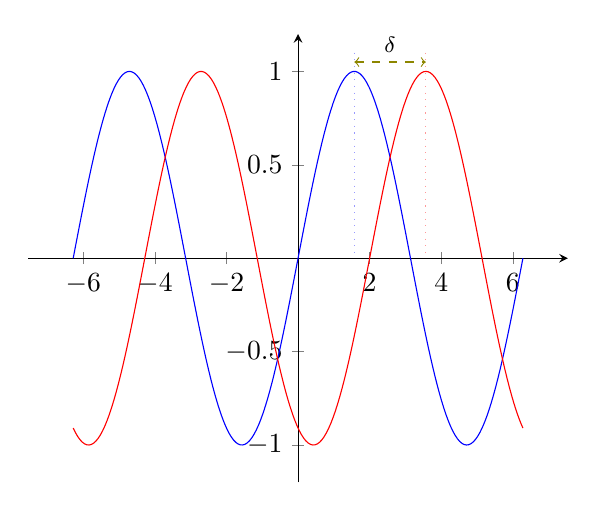
\begin{tikzpicture}
	  	\begin{axis}[
	    trig format plots=rad,
	    axis lines = middle,
	    enlargelimits,
	    clip=false
	    ]
	    \addplot[domain=-2*pi:2*pi,samples=200,blue] {sin(x)};
	    \addplot[domain=-2*pi:2*pi,samples=200,red] {sin(x-2)};
	    \draw[dotted,blue!40] (axis cs: 0.5*pi,1.1) -- (axis cs: 0.5*pi,0);
	    \draw[dotted,red!40] (axis cs: 0.5*pi+2,1.1) -- (axis cs: 0.5*pi+2,0);
	    \draw[dashed,olive,<->] (axis cs: 0.5*pi,1.05) -- node[above,text=black,font=\footnotesize]{$\delta$}(axis cs: 0.5*pi+2,1.05);
	  	\end{axis}
		\end{tikzpicture}
	\end{figure}
	\end{tcolorbox}
	En utilisant les propri\'et\'es des fonctions trigonom\'etriques:
	
	Suivant que nous sommons ou soustrayons cela nous donne les "\NewTerm{formules d'Euler}" ou "\NewTerm{formules de Moivre et Euler}\index{formules de Moivre et Euler}\label{de Moivre and Euler formulas}":
	
	Remarquons que l'angle peut être un nombre purement complexe et dans ce cas les deux formules d'Euler donnent un nombre r\'eel. Si l'angle est un nombre complexe avec une partie r\'eelle plus imaginaire alors dans ce cas les fonctions trigonom\'etriques redonnent un nombre complexe en sortie. Ceci pour dire qu'en toute g\'en\'eralit\'e les fonctions trigonom\'etriques peuvent être consid\'er\'ees commes des fonctions qui vont de $\mathbb{C}$ dans $\mathbb{C}$.
	\begin{tcolorbox}[title=Remarque,colframe=black,arc=10pt]
	Notez que ces relations sont très utiles pour lin\'eariser des expressions telles que $\cos^k(\theta)$ ou $\sin^k(\theta)$. Effectivement:
	
	\end{tcolorbox}
	Un cas particulier bien connu pour les formules ci-dessus est le cas où $\varphi=\pi$ et $r=1$. Nous avons alors:
	
	après r\'earrangement, nous obtenons la fameuse relation que de nombreux "geek" connaissent:
	
	Un autre cas c\'elèbre est celui où nous prenons encore $r=1 $ mais avec $\varphi=\pi/2$ et que nous \'elevons à la puissance de $\mathrm{i}$. Nous obtenons alors:
	
	et si nous \'elevons cela à la puissance de $\mathrm{i}$:
	
	Certaines personnes considèrent alors comme un fait curieux que $\mathrm{i}$  \'elev\'e à la puissance $\mathrm{i}$ donne un nombre r\'eel.
	
	Grâce à la forme exponentielle d'un nombre complexe, très fr\'equemment utilis\'ee dans de nombreux domaines de la physique et de l'ing\'enierie, nous pouvons très facilement tirer des relations telles que ($\text{cis}$ est une vieille notation qui est l'abr\'eviation du $\cos(\varphi)+\mathrm{i}\sin(\varphi)$ se trouvant dans la parenthèse):
	
	et en supposant connues les relations trigonom\'etriques de bases (\SeeChapter{voir section de Trigonom\'etrie page \pageref{remarkable trigonometric identities}}) nous avons les relations suivantes pour la multiplication de deux nombres complexes:
	
	dès lors:
	
	et donc si $n$ est un entier positif:
	
	Pour le module de la multiplication (nous changeons de notation pour la lisibilit\'e): 
	
	d'où:
	
	Pour la division de deux nombres complexes:
	
	Le module de leur division vient alors imm\'ediatement:
	
	dès lors nous avons pour l'argument:
	
	ainsi il vient imm\'ediatement:
	
	Pour la mise en puissance d'un nombre complexe (ou la racine):
	
	ce qui nous donne imm\'ediatement un r\'esultat d\'ejà mentionn\'e plus haut: 
	
	et pour l'argument:
	
	Dans le cas où nous avons un module unit\'e (norme \'egale à $1$)  tel que $z=\cos(\varphi)+\mathrm{i}\sin(\varphi)$ nous avons alors la relation:
	
	appel\'ee "\NewTerm{formule de Moivre}\index{formule de Moivre}".

	Pour le logarithme n\'ep\'erien d'un nombre complexe, nous avons trivialement la relation suivante sur laquelle nous reviendrons dans le chapitre d'Analyse Complexe (page \pageref{logarithms}):
	
	où $\ln(z)$ est souvent dans le cas complexe \'ecrit $\mathrm{Log}(z)$ avec un "L" majuscule.
	 
	Toutes les relations pr\'ec\'edentes pourraient bien sûr être obtenues avec la forme trigonom\'etrique des nombres complexes mais n\'ecessiteraient alors quelques lignes suppl\'ementaires de d\'eveloppements.
	
	\begin{tcolorbox}[title=Remarques,colframe=black,arc=10pt]
	Notez que les d\'eveloppements pr\'ec\'edents nous autorisent à calculer des choses (..) du genre $\cos(\bar{z})$. Effectivement, posons $z=x+\mathrm{i}y$ et consid\'erons:
	
	Similairement, nous avons:
	
	Maintenant consid\'erons:
	
	\end{tcolorbox}
	
	\subparagraph{Vecteurs de Fresnel (phaseurs)}\mbox{}\\\\
	Une variation sinusoïdale $f(t)=r\sin(\omega t)$ peut être repr\'esent\'ee comme la projection (\SeeChapter{voir section de Trigonom\'etrie page \pageref{trigonometry}}) sur l'axe vertical $y$ (axe des imaginaires de l'ensemble $\mathbb{C}$) d'un vecteur $\vec{r}$ tournant à vitesse angulaire $\omega$ autour de l'origine dans le plan $x\text{O}y$:
	\begin{figure}[H]
		\centering
		\includegraphics{img/arithmetics/fresnel_representation.jpg}
		\caption{Repr\'esentation de Fresnel}
	\end{figure}
	Un tel vecteur tournant s'appelle "\NewTerm{vecteur de Fresnel}\index{vecteur de Fresnel}" et peut très bien être interpr\'et\'e comme la partie imaginaire d'un nombre complexe donn\'e par:
	
	C'est-à-dire:
	\begin{figure}[H]
		\centering
		\includegraphics{img/arithmetics/fresnel_rotating_vector.jpg}
		\caption{Vecteur tournant de Fresnel}
	\end{figure}
	Nous retrouverons les vecteurs tournants de façon explicite lors de notre \'etude de la m\'ecanique ondulatoire et optique g\'eom\'etrique (dans le cadre de la diffraction) dans les sections correspondantes aux pages respectives \pageref{wave mechanics} et \pageref{geometrical optics}.
	
	\paragraph{Transformations dans le plan}\mbox{}\\\\
	Il est habituel de repr\'esenter les nombres r\'eels comme points d'une droite gradu\'ee. Les op\'erations alg\'ebriques y ont leur interpr\'etation g\'eom\'etrique: l'addition est une translation, la multiplication une homoth\'etie centr\'ee à l'origine.
	
	En particulier nous pouvons parler de la "racine carr\'ee d'une transformation". Une translation d'amplitude $T$ peut être obtenue comme l'it\'eration d'une translation d'amplitude  $T / 2$. De même une homoth\'etie de rapport $S$ peut être obtenue comme l'it\'er\'ee d'une homoth\'etie de rapport $\sqrt{S}$. En particulier une homoth\'etie de rapport $9$ est la compos\'ee de deux homoth\'eties de rapport $3$ (ou $-3$).
	
	La racine carr\'ee prend alors un sens g\'eom\'etrique. Mais qu'en est-il de la racine carr\'ee de nombres n\'egatifs?  En particulier de la racine carr\'ee de $-1$?
	
	Une homoth\'etie de rapport $-1$ peut être vue comme une sym\'etrie par rapport à l'origine. Toutefois si nous voulons voir cette transformation d'une manière continue, force nous est de placer la droite dans un plan. Dès lors une homoth\'etie de rapport $-1$ peut être vue comme une rotation de $\pi$ radians autour de l'origine.
	
	Du coup, le problème de la racine carr\'ee n\'egative se simplifie. En effet, il n'est guère difficile de d\'ecomposer une rotation de $\pi$ radians en deux transformations: nous pouvons r\'ep\'eter soit une rotation de $\pi/2$ soit une rotation de $-\pi/2$. L'image de $1$ sera la racine carr\'ee de $-1$ et $\mathrm{i}$ est situ\'ee sur une perpendiculaire à l'origine à une distance $1$ soit vers le haut soit vers le bas.
	
	Ayant r\'eussi à positionner le nombre  $\mathrm{i}$ il n'est plus guère difficile de disposer les autres nombres complexes dans un plan de Gauss. Nous pouvons ainsi associer à $2\mathrm{i}$ le produit de l'homoth\'etie (\SeeChapter{voir section de G\'eom\'etrie Euclidenne page \pageref{scaling}}) de rapport $2$ par la rotation de centre O et d'angle $\pi/2$, soit une similitude centr\'ee à l'origine. C'est ce que nous allons nous efforcer à montrer maintenant.
	
	Soient:
	
	Nous avons les propri\'et\'es de transformations g\'eom\'etriques suivantes pour les nombres complexes (voir le chapitre de Trigonom\'etrie pour les propri\'et\'es du sinus et cosinus) que nous pouvons joyeusement combiner selon notre bon vouloir:
	\begin{enumerate}
		\item[P1.] La multiplication de $z_1$ par un r\'eel $\lambda$ dans le plan de Gauss correspond (trivial) à une homoth\'etie (agrandissement) de centre O (l'intersection des axes imaginaires et r\'eels), de rapport $\lambda$.
		
		Effectivement:
		
		
		\item[P2.] La multiplication de $z_1$  par un nombre complexe de module unitaire correspond à une rotation de centre 0 et à un angle correspondant à l'argument de $z_1$. Effectivement:
		
		\begin{tcolorbox}[title=Remarque,colframe=black,arc=10pt]
		Nous voyons alors imm\'ediatement, par exemple, que multiplier un nombre complexe par $\mathrm{i}$ (c'est-à-dire $ \sin(\omega)=1,\cos(\omega)=0$) correspond à une rotation de $\pi/2$.
		\end{tcolorbox}
		\begin{theorem}
		Il est int\'eressant d'observer que sous forme vectorielle la rotation de centre O de $z_1$ par  $z_0$ peut s'\'ecrire à l'aide de la matrice suivante:
		
		\end{theorem}
		\begin{dem}
		Nous savons que $z_0z_1$ est une rotation de centre O et d'angle $\omega$. Il suffit de l'\'ecrire à l'ancienne:
		
		ce qui donne sous forme vectorielle:
		
		donc l'application lin\'eaire est \'equivalente à:
		
		ou encore (nous retombons sur la matrice de rotation dans le plan que nous avons dans le chapitre de G\'eom\'etrie Euclidienne page \pageref{rotation matrix in the plane} ce qui est un r\'esultat remarquable!) en utilisant:
		
		dans le cas particulier et arbitraire où $r$ serait unitaire (afin d'avoir une rotation pure!):
		
		nous avons imm\'ediatement (nous avons repris les notations de l'angle tel que nous l'avons dans le chapitre de G\'eom\'etrie):
		
		Remarquons que la matrice de rotation 2D peut aussi s'\'ecrire sous la formes\label{2d rotation matrix}:
		
		de même:
		
		\begin{flushright}
			$\blacksquare$  Q.E.D.
		\end{flushright}
		\end{dem}
		Ainsi nous remarquons que ces matrices de rotation ne sont pas que des applications mais sont des nombres complexes aussi (bon c'\'etait \'evident dès le d\'ebut mais fallait le montrer de manière esth\'etique et simple).
		
		Ainsi, nous avons pour habitude de poser que:
		
		ou avec une autre notation fr\'equente en alègbre lin\'eaire:
		
		Le corps des nombres complexes est donc isomorphe au corps des matrices r\'eelles carr\'ees de dimension $2$ du type:
		
		C'est un r\'esultat que nous r\'eutiliserons de nombreuses fois dans divers chapitres de ce site pour des \'etudes particulières en algèbre, g\'eom\'etrie et en physique quantique relativiste.
		
		\item[P3.] La multiplication de deux complexes correspond à une homoth\'etie ajout\'ee à une rotation. En d'autres termes, d'une "\NewTerm{similitude directe}\index{similitude directe}".
		\begin{dem}
		
		il s'agit donc bien d'une similitude de rapport $b$ et d'angle  $\beta$.
		
		Au contraire, l'op\'eration suivante:
		
		sera appel\'ee une "\NewTerm{similitude lin\'eaire r\'etrograde}\index{similitude lin\'eaire r\'etrograde}".
		
		Par ailleurs, il en retourne trivialement la relation d\'ejà connue suivante:
		
		\begin{tcolorbox}[title=Remarques,colframe=black,arc=10pt]
		\textbf{R1.} La somme de deux nombres $z_1+z_2$ complexes ne pouvant avoir une \'ecriture math\'ematique simplifi\'ee sous quelque forme que ce soit, nous disons alors que la somme \'equivaut à une "\NewTerm{translation d'amplitude}\index{translation d'amplitude}".\\
		
		\textbf{R2.}  La combinaison d'une similitude lin\'eaire (multiplication de deux nombres complexes) directe et d'une translation d'amplitude (sommation par un troisième nombre complexe) correspond à ce que nous appelons une "\NewTerm{similitude lin\'eaire directe}\index{similitude lin\'eaire directe}".
		\end{tcolorbox}
		\begin{flushright}
			$\blacksquare$  Q.E.D.
		\end{flushright}
		\end{dem}
		
		\item[P4.] Le conjugu\'e d'un nombre complexe est g\'eom\'etriquement son sym\'etrique par rapport à l'axe r\'e\'el tel que:
		
		sans oublier que (trigonom\'etrie de base):
		
		Ce qui nous donne un r\'esultat d\'ejà connu:
		
		D'où nous pouvons tirer la propri\'et\'e suivante:
		
		d'où:
		
		
		\item[P5.] La n\'egation du conjugu\'e d'un nombre complexe est g\'eom\'etriquement son sym\'etrique par rapport à l'axe des imaginaires tel que:
		
		\begin{tcolorbox}[title=Remarques,colframe=black,arc=10pt]
		\textbf{R1.} La combinaison des propri\'et\'es P4, P5 est appel\'ee une "\NewTerm{similitude r\'etrograde}\index{similitude r\'etrograde}".\\
		
		\textbf{R2.} L'op\'eration g\'eom\'etrique qui consiste à prendre l'inverse du conjugu\'e d'un nombre complexe (soit  $\bar{z}^{-1}$) est appel\'ee une "\NewTerm{inversion de pôle}\index{inversion de pôle}".
		\end{tcolorbox}
		
		\item[P6.] La rotation de centre $c$ et d'angle $\varphi$ est donn\'ee par:
		
		Explications:
		
		Le complexe $c$ donne un point dans le plan de Gauss qui sera le centre de rotation. La diff\'erence $z_1-c$ donne le rayon $r$ choisi. La multiplication par $e^{\mathrm{i}\varphi}$ est la rotation du rayon par rapport à l'origine du plan de Gauss dans le sens inverse des aiguilles d'une montre. Finalement, l'addition par $c$ est la translation n\'ecessaire pour ramener le rayon $r$ tourn\'e à l'origine du centre $c$. Ce qui donne sch\'ematiquement:
		\begin{figure}[H]
			\centering
			\includegraphics{img/arithmetics/complex_rotation.jpg}
			\caption{Repr\'esentation de la rotation complexe}
		\end{figure}
	
		\item[P7.] Sur la même id\'ee, nous obtenons une homoth\'etie de centre $c$, de rapport $\lambda$ par l'op\'eration:
		
		Explications:
		
		La diff\'erence $z_1-c$ donne toujours le rayon $r$ et $c$ un point dans le centre de Gauss. L'expression $\lambda(z_1-c)$ donne l'homoth\'etie du rayon par rapport à l'origine du plan de Gauss et finalement l'addition par $c$ la translation n\'ecessaire pour que l'homoth\'etie soit vue comme \'etant faite de centre $c$.
	\end{enumerate}
	
	\subsubsection{Nombres Quaternions}\label{quaternions}
	Appel\'es aussi "\NewTerm{hypercomplex}\index{hypercomplex}", les nombres quaternions ont \'et\'e invent\'es en 1843 par William Rowan Hamilton pour g\'en\'eraliser les nombres complexes.
	
	\textbf{D\'efinition (\#\mydef):} Un "\NewTerm{quaternion}\index{quaternion}" est un \'el\'ement $(a,b,c,d)\in \mathbb{R}^4$ et dont nous notons $\mathbb{H}$ l'ensemble qui le contient et que nous appelons "\NewTerm{ensemble des quaternions}\index{ensemble des quaternions}".
	
	Un quaternion peut aussi bien être repr\'esent\'e en ligne ou en colonne tel que:
	
	Nous d\'efinissons la somme de deux quaternions $(a, b, c, d)$ et $(a ', b', c ', d')$ par:
	
	Il est \'evident (du moins nous l'esp\'erons pour le lecteur) que $(\mathbb{H},+)$ est un groupe commutatif (\SeeChapter{voir section Th\'eorie des Ensembles page \pageref{commutative field}}), d'\'el\'ement neutre $(0,0,0,0)$, l'oppos\'e d'un \'el\'ement $(a,b,c,d)$ \'etant $(-a,-b,-c,-d)$. 
	
	L'associativit\'e se v\'erifie en appliquant les propri\'et\'es correspondantes des op\'erations sur $\mathbb{R}$.
	
	Nous d\'efinissons \'egalement la multiplication:
	
	de deux quaternions $(a, b, c, d)$ et $(a', b', c', d')$ par l'expression:
	
	C'est peut-être difficile à accepter mais nous verrons un peu plus loin qu'il y a un air de famille avec les nombres complexes.

	Nous pouvons remarquer que la loi de multiplication n'est pas commutative. Effectivement, en prenant la d\'efinition de la multiplication ci-dessus, nous avons:
	
	Mais nous pouvons aussi remarquer que:
	
	
	\begin{tcolorbox}[title=Remarque,colframe=black,arc=10pt]
	C'est l'addition naturelle dans $\mathbb{R}^4$ vu comme un $\mathbb{R}$-espace vectoriel ((\SeeChapter{voir section Th\'eorie des Ensembles page \pageref{vector space}}).
	\end{tcolorbox}
	
	La loi de multiplication est distributive avec la loi d'addition mais c'est un excellent exemple où il faut quand même prendre garde à d\'emontrer la distributivit\'e à gauche et à droite, puisque le produit n'est pas commutatif !
	
	La multiplication a pour \'el\'ement neutre:
	
	Effectivement:
	
	Tout \'el\'ement:
	
	est inversible.
	
	En effet, si $(a,b,c,d)$ est un quaternion non nul, nous avons alors n\'ecessairement:
	
	sinon les quatre nombres $a, b, c, d$ sont de carr\'e nul, donc tous nuls. Soit alors le quaternion $(a_1,b_1,c_1,d_1)$ d\'efini par:
	
	alors en appliquant machinalement la d\'efinition de la multiplication des quaternions, nous v\'erifions que:
	
	ce dernier quaternion est donc l'inverse pour la multiplication!
	
	Montrons maintenant (pour la culture g\'en\'erale) que le corps des complexes equation est un sous-corps de $(\mathbb{H},+,\times)$.
	\begin{tcolorbox}[title=Remarque,colframe=black,arc=10pt]
	Nous aurions pu mettre cette d\'emonstration dans le chapitre de Th\'eorie Des Ensembles car nous faisons usage de beaucoup de concepts qui y sont vus mais il nous a sembl\'e un peu plus pertinent de la mettre ici.
	\end{tcolorbox}
	Soit $\mathbb{H}'$ l'ensemble des quaternions de la forme $(a, b, 0,0)$. Si $\mathbb{H}'$ est non vide, et si $(a, b, 0,0)$, $(a ', b', 0.0)$ sont des \'el\'ements de $\mathbb{H}'$ alors $(\mathbb{H}',+\times)$ est un corps. Effectivement:
	\begin{enumerate}
		\item[P1.] Pour la soustraction (et donc l'addition):
		

		\item[P2.] La multiplication:
			

		\item[P3.] L'\'el\'ement neutre:
		

		\item[P4.] Et finalement l'inverse:
		
		de $(a,b,0,0)$ est encore dans $\mathbb{H}'$.
	\end{enumerate}
	Donc $(\mathbb{H}',+,\times)$ est un sous-corps de $\mathbb{H}$. Soit alors l'application:
	
	$f$ est bijective, et nous v\'erifions ais\'ement que pour tous complexes $z_1,z_2$, nous avons:
	
	Donc $f$ est un isomorphisme de $(\mathbb{C},+,\times)$ sur $(\mathbb{H}',+,\times)$.
	
	Cet isomorphisme a pour int\'erêt (provoqu\'e) d'identifier $\mathbb{C}$ à $\mathbb{H}'$ et d'\'ecrire $\mathbb{C} \subset\mathbb{H}$, les lois d'addition et de soustraction sur $\mathbb{H}$ prolongeant les op\'erations d\'ejà connues sur $\mathbb{C}$.
	
	Ainsi, par convention, nous \'ecrirons tout \'el\'ement de $(a, b, 0,0)$ de $\mathbb{H}'$ sous la forme complexe $a + \mathrm{i}b$. En particulier $0$ est l'\'el\'ement $(0,0,0,0)$, $1$ est l'\'el\'ement $(1,0,0,0)$ et $\mathrm{i}$ est l'\'el\'ement $(0,1,0,0)$.
	
	Nous notons par analogie et par extension $\mathrm{j}$ l'\'el\'ement  $(0,0,1,0)$ et $\mathrm{k}$ l'\'el\'ement $(0,0,0,1)$. La famille $\{1, \mathrm{i}, \mathrm{j}, \mathrm{k}\}$ forme une base de l'ensemble des quaternions vu comme un espace vectoriel sur $\mathbb{R}$, et nous \'ecrirons:
	
	le quaternion $(a, b, c, d)$.

	La notation des quaternions sous forme d\'efinie ci-avant est parfaitement adapt\'ee à l'op\'eration de multiplication. Pour le produit de deux quaternions nous obtenons en d\'eveloppant l'expression:
	
	$16$ termes que nous devons identifier à la d\'efinition d'origine de la multiplication des quaternions pour obtenir les relations suivantes:
	
	Ce qui peut se r\'esumer dans un tableau:
	

	Ou dans une repr\'esentation 3D de ce qu'il se passe dans la sphère 4D correspondante (rouge, vert et bleu pour $\mathrm{i}$, $\mathrm{j}$ et $\mathrm{k}$ respectivement):
	\begin{figure}[H]
		\centering
		\includegraphics{img/arithmetics/quaternions_3D_4D_sphere_representation.jpg}
		\caption[]{Situation de d\'epart pour rotation des quaternions}
	\end{figure}
	Nous pouvons constater que l'expression de la multiplication de deux quaternions ressemble en partie beaucoup à un produit vectoriel (not\'e $\circ$ dans ce livre) et scalaire (not\'e equation sur ce site):
	
	Si ce n'est pas \'evident (ce qui serait tout à fait compr\'ehensible), faisons un exemple concret:
	\begin{tcolorbox}[colframe=black,colback=white,sharp corners]
	\textbf{{\Large \ding{45}}Exemple:}\\\\
	Soient deux quaternions sans partie r\'eelle:
	
	et $\vec{u},\vec{v}$ les vecteurs de $\mathbb{R}^3$  de coordonn\'ees respectives $(x,y,z)$ et $(x',y',z')$. Alors le produit:
	
	est \'egal à:
	
	Nous pouvons aussi par curiosit\'e nous int\'eresser au cas g\'en\'eral... Soient pour cela deux quaternions:
	
	Nous avons alors:
	
	\end{tcolorbox}
	\textbf{D\'efinition (\#\mydef):} Le centre du corps non-commutatif $(\mathbb{H},+,\times)$ est l'ensemble des \'el\'ements de $\mathbb{H}$ commutant pour la loi de multiplication avec tous les \'el\'ements de $\mathbb{H}$.

	\begin{theorem}
	Le centre de $(\mathbb{H},+,\times)$ est l'ensemble des r\'eels!
	\end{theorem}
	\begin{dem}
	Soit $\mathbb{H}_1$ le centre de $(\mathbb{H},+,\times)$, et $(x, y, z, t)$ un quaternion. Nous devons avoir les conditions suivantes qui soient satisfaites:

	Soit  $(x,y,z,t)\in \mathbb{H}_1 $  alors pour tout $(a,b,c,d)\in \mathbb{H}$ nous cherchons:
	
	ce qui donne en d\'eveloppant:
	
	après simplification (la première ligne du système pr\'ec\'edent est nulle des deux côt\'es de l'\'egalit\'e):
	
	la r\'esolution de ce système, nous donne:
	
	Donc pour que le quaternion $(x, y, z, t)$ soit le centre de $\mathbb{H}$ il doit être r\'eel (sans parties imaginaires)!
	\begin{flushright}
		$\blacksquare$  Q.E.D.
	\end{flushright}
	\end{dem}
	Au même titre que pour les nombres complexes, nous pouvons d\'efinir un conjugu\'e des quaternions:
	
	\textbf{D\'efinition (\#\mydef):} Le conjugu\'e d'un quaternion $Z=(a,b,c,d)$ est le quaternion $\bar{Z}=(a,-b,-c,-d)$.

	Au même titre que pour les complexes, nous remarquons que:
	\begin{enumerate}
		\item D'abord de manière \'evidente que si $Z=\bar{Z}$ alors cela signifie que $Z\in \mathbb{R}$.

		\item Que $Z+\bar{Z}\in \mathbb{R}$

		\item Qu'en d\'eveloppant le produit $Z\bar{Z}$ nous avons:
		
		que nous adopterons, par analogie avec les nombres complexes, comme une d\'efinition de la norme (ou module) des quaternions tel que:
		
		Dès lors nous avons aussi imm\'ediatement (relation qui nous sera utile plus tard):
		
	\end{enumerate}
	Comme pour les nombres complexes (voir plus loin), il est ais\'e de montrer que la conjugaison est un automorphisme du groupe $(\mathbb{H},+)$.
	
	Effectivement, soient $Z=(a,b,c,d)$ et $Z'=(a',b',c',d')$ alors:
	
	Il est aussi ais\'e de d\'emontrer qu'elle est involutive. Effectivement:
	
	La conjugaison n'est par contre pas un automorphisme multiplicatif du corps $(\mathbb{H},+,\times)$. En effet, si nous consid\'erons la multiplication de $Z$ et $Z'$ et en prenons le conjugu\'e:
	
	nous voyons imm\'ediatement (ne serait-ce que pour la deuxième ligne) que nous avons:
	
	Revenons maintenant sur notre norme (ou module).... Pour cela, calculons le carr\'e de la norme de $|ZZ'|$:
	
	Nous savons (par d\'efinition) que:
	
	notons ce produit de manière telle que:
	
	Nous avons alors:
	
	en substituant il vient:
	
	après un d\'eveloppement alg\'ebrique \'el\'ementaire (honnêtement ennuyeux), nous trouvons:
	
	Donc:
	
	\begin{tcolorbox}[title=Remarque,colframe=black,arc=10pt]
	La norme est donc un homomorphisme de $(\mathbb{H},\times)$ dans $(\mathbb{R},\times)$. Par la suite, nous noterons $\mathbb{G}$ l'ensemble des quaternions de norme unitaire.
	\end{tcolorbox}
	
	\paragraph{Interpr\'etation matricielles des quaternions}\mbox{}\\\\
	Soient $q$ et $p$ deux quaternions donn\'es, soit l'application:
	
	La multiplication (à gauche) peut être faite avec une application lin\'eaire (\SeeChapter{voir section d'Algèbre Lin\'eaire page \pageref{linear application}}) sur $\mathbb{H}$.
	
	Si $q$ s'\'ecrit:
	
	cette application a pour matrice, dans la base $(1,\mathrm{i},\mathrm{j},\mathrm{k})$:
	
	Ce que nous v\'erifions bien:
	
	En fait, nous pouvons alors d\'efinir les quaternions comme l'ensemble des matrices ayant la structure visible ci-dessus si nous le voulions. Cela les r\'eduirait alors à un sous espace vectoriel de $M_4(\mathbb{R})$.
	
	En particulier, la matrice de $1$  (la partie r\'eelle du quaternion $q$) n'est alors rien d'autre que la matrice identit\'e:
	
	de même:
	
	
	\paragraph{Rotations avec les quaternions}\mbox{}\\\\
	Nous allons maintenant voir que la conjugaison par un \'el\'ement du groupe $\mathbb{G}$ des quaternions de norme unit\'e peut s'interpr\'eter comme une rotation pure dans l'espace!
	
	\textbf{D\'efinition (\#\mydef):} La "\NewTerm{conjugaison}\index{conjugaison}" par un quaternion $q$ non nul et de norme unit\'e est l'application $S_q$ d\'efinie sur $\mathbb{H}$ par:
	
	et nous affirmons que cette application est une rotation.
	
	\begin{tcolorbox}[title=Remarques,colframe=black,arc=10pt]
	\textbf{R1.}  Comme $q$ est de norme $1$, nous avons bien \'evidemment $|q|=q\bar{q}=1$ donc $q^{-1}=\bar{q}$. Ce quaternion peut être vu comme la valeur propre (unitaire) de l'application (matricielle) $p$ sur le vecteur  $\bar{q}$ (on se retrouve avec un concept en tout point similaire aux matrices orthogonales de rotation vues dans la section d'Algèbre Lin\'eaire page \pageref{orthogonal matrix}).\\
	
	\textbf{R2.} $S_q$ est une application lin\'eaire (donc si c'est bien une rotation, la rotation peut être d\'ecompos\'ee en plusieurs rotations). Effectivement, prenons deux quaternions $p_1,p_2$  et deux r\'eels $\lambda_1,\lambda_2$, alors nous avons:
	
	\end{tcolorbox}
	V\'erifions maintenant que l'application est bien une rotation pure. Comme nous l'avons vu lors de notre \'etude de l'algèbre lin\'eaire et en particulier des matrices orthogonales (\SeeChapter{voir section d'Algèbre Lin\'eaire page \pageref{orthogonal matrix}}), une première condition est que l'application conserve la norme.
	
	V\'erifions cela:
	
	Par ailleurs, nous pouvons v\'erifier qu'une rotation d'un quaternion purement complexe (tel qu'alors nous nous restreignons à $\mathbb{R}^3$) et la même rotation inverse somm\'ees est nulle (le vecteur somm\'e à son oppos\'e s'annulent):
	
	nous v\'erifions trivialement que si nous avons deux quaternions $q, p$ alors $\overline{p\cdot q}=\bar{q}\bar{p}$ dès lors:
	
	pour que cette op\'eration soit nulle, nous voyons imm\'ediatement que nous devons restreindre $p$ aux quaternions purement complexes. Dès lors:
	
	Nous en d\'eduisons alors que $p$ doit être purement complexe pour que l'application $S_q$ soit une rotation et que $S_q(p)$  est un quaternion pur. En d'autres termes, cette application est stable (en d'autres termes: un quaternion pur par cette application reste un quaternion pur).
	
	$S_q$ restreint à l'ensemble des quaternions purement complexes est donc une isom\'etrie vectorielle, c'est-à-dire une sym\'etrie ou une rotation.
	
	Nous avons vu \'egalement lors de notre \'etude des matrices de rotation dans la section d'Algèbre Lin\'eaire page \pageref{rotation matrix in linear algebra} que d telles matrices devaient avoir un d\'eterminant de $+1$ pour que nous ayons une rotation. Voyons si c'est le cas de $S_q$:
	
	Pour cela, nous calculons explicitement en fonction de:
	
	la matrice (dans la base canonique $(\mathrm{i},\mathrm{j},\mathrm{k})$) de $S_q$ et nous en calculons le d\'eterminant. Ainsi, nous obtenons les coefficients des colonnes en se rappelant que:
	
	et ensuite en calculant:
	
	
	
	
	
	Il faut alors calculer le d\'eterminant de la matrice (pfff...):
	
	en se souvenant que (ce qui permet aussi de simplifier l'expression des termes de la diagonale comme nous pouvons le voir dans certains ouvrages):
	
	nous trouvons que le d\'eterminant vaut bien $1$. Sinon, nous pouvons v\'erifier cela avec Maple 4.00b:
	
	\texttt{>with(linalg):\\
	>A:=linalg[matrix](3,3,[a\string^2+b\string^2-c\string^2-d\string^2,2*(a*d+b*c),\\
	2*(b*d-a*c),2*(b*c-a*d),a\string^2-b\string^2+c\string^2-d\string^2,2*(a*b+c*d),\\
	2*(a*c+b*d),2*(c*d-a*b),a\string^2-b\string^2-c\string^2+d\string^2]);\\
	>factor(det(A));}
	
	Montrons maintenant que cette rotation est un demi-tour d'axe (l'exemple qui peut sembler particulier est g\'en\'eral!):
	
	D'abord, si:
	
	nous avons:
	
	ce qui signifie que l'axe de rotation $(x, y, z)$ est fix\'e par l'application $S_q$ elle-même !
	
	D'autre part, nous avons vu que si $q$ est un quaternion purement complexe de norme $1$ alors:
	
	Ce qui nous donne la relation:
	
	Ce r\'esultat nous amène à calculer la rotation d'une rotation:
	
	Conclusion: Puisque la rotation d'une rotation est un tour complet, alors $S_q$ est n\'ecessairement un demi-tour:
	
	relativement (!) aux axes $(x, y, z)$.
	
	À ce stade, nous pouvons affirmer que toute rotation de l'espace peut se repr\'esenter par $S_q$ (la conjugaison par un quaternion $q$ de norme $1$). En effet, les demi-tours engendrent le groupe des rotations, c'est-à-dire que toute rotation peut s'exprimer comme le produit d'un nombre fini de demi-tours, et donc comme la conjugaison par un produit de quaternions de norme unitaire (produit qui est lui-même un quaternion de norme unitaire ...).
	
	Nous allons tout de même donner une forme explicite reliant une rotation et le quaternion qui la repr\'esente, au même titre que nous l'avons fait pour les nombres complexes.
	\begin{theorem}
	Soit $\vec{u}(x,y,z)$ un vecteur unitaire et $\theta \in [0,2\pi]$ un angle. Alors nous affirmons que la rotation d'axe $\vec{u}$ et d'angle $\theta$ correspond à l'application $S_q$, où $q$ est le quaternion:
	
	Pour que cette affirmation soit v\'erifi\'ee, nous savons qu'il faut que:
	\begin{itemize}
		\item La norme de $q$ soit unitaire $1$

		\item Le d\'eterminant de l'application $S_q$ soit \'egal à l'unit\'e $1$

		\item Que l'application $S_q$ conserve la norme
	
		\item Que l'application $S_q$ renvoie tout vecteur colin\'eaire à l'axe de rotation sur l'axe de rotation
	\end{itemize}
	\end{theorem}
	\begin{dem}
	Ok contrôlons chacun de ces points!
	\begin{enumerate}
		\item La norme du quaternion propos\'e pr\'ec\'edemment vaut effectivement $1$:
		
		et comme $\vec{u}(x,y,z)$ est unitaire alors nous avons:
		
		Donc:
		
		
		\item Le fait que $q$ soit un quaternion de norme unitaire amène imm\'ediatement à ce que le d\'eterminant de l'application equation soit unitaire. Nous l'avons d\'ejà montr\'e plus haut dans le cas g\'en\'eral de n'importe quel quaternion de norme $1$ (condition n\'ecessaire et suffisante).
		
		\item Il en est de même pour la conservation de la norme. Nous avons d\'ejà montr\'e plus haut que c'\'etait de toute façon le cas dès que le quaternion $q$ \'etait de norme $1$ (condition n\'ecessaire et suffisante).

		\item Voyons maintenant que tout vecteur colin\'eaire à l'axe de rotation est projet\'e sur l'axe de rotation. Notons $q'$ le quaternion purement imaginaire et unitaire $x\mathrm{i}+y\mathrm{j}+z\mathrm{k}$. Nous avons alors:
		
		Alors:
		
		mais comme $q'$ est la restriction de $q$ à ces \'el\'ements purs qui le constituent, cela revient à \'ecrire:
		
		Montrons maintenant le choix de l'\'ecriture $\theta/2$. Si $\vec{v}=(x_1,y_1,z_1)$ d\'esigne un vecteur unitaire orthogonal à equation (perpendiculaire à l'axe de rotation donc), et $p$  le quaternion $x\mathrm{i}+y\mathrm{j}+z\mathrm{k}$ alors nous avons:	
		
		Nous avons montr\'e lors de la d\'efinition de la multiplication de deux quaternions que:
		
		nous obtenons alors:
		
		Nous avons \'egalement d\'emontr\'e plus haut que:
		
		dès lors:
		
		(le demi-tour d'axe $(x, y, z)$). Donc:
		
		\begin{tcolorbox}[title=Remarque,colframe=black,arc=10pt]
		Nous commençons à entrevoir ici d\'ejà l'utilit\'e d'avoir \'ecrit dès le d\'ebut $\theta/2$ pour l'angle!
		\end{tcolorbox}
	\end{enumerate}
	\begin{flushright}
		$\blacksquare$  Q.E.D.
	\end{flushright}
	\end{dem}
	Nous savons que $p$ est le quaternion pur assimil\'e à un vecteur unitaire $\vec{v}$ orthogonal à l'axe de rotation $\vec{u}$, lui-même assimil\'e à la partie purement imaginaire de $q'$. Nous remarquons alors de suite que la partie imaginaire du produit (d\'efini!) des quaternions $q'p$ est alors \'egal au produit vectoriel $\vec{u}\times\vec{v}=\vec{w}$. Ce produit vectoriel engendre donc un vecteur perpendiculaire à $\vec{u},\vec{v}$.
	
	Le couple $(\vec{v},\vec{w})$ forme donc un plan perpendiculaire à l'axe de rotation $\vec{u}$ (c'est comme pour les nombres complexes simples $\mathbb{C}$ dans lequel nous avons le plan de Gauss et perpendiculairement à celui-ci un axe de rotation!).
	
	Alors finalement:
	
	Nous nous retrouvons avec une rotation bas\'ee sur un plan (mais qui a donc lieu dans l'espace!) identique à celle pr\'esent\'ee plus haut avec les nombres complexes standards dans le plan de Gauss. Pour plus de d\'etails le lecteur peut se r\'ef\'erer à la section sur le Calcul Spinoriel à la page \pageref{spinors}.
	
	Nous savons donc maintenant comment faire n'importe quel type de rotation dans l'espace en une seule op\'eration math\'ematique et ce en plus par rapport à un libre choix de l'axe !

	Nous pouvons aussi maintenant mieux comprendre pourquoi l'algèbre des quaternions n'est pas commutative. Effectivement, les rotations vectorielles du plan sont commutatives mais celles de l'espace ne le sont pas comme nous le montre l'exemple ci-dessous:

	Soit la configuration initiale:
	\begin{figure}[H]
		\centering
		\includegraphics{img/arithmetics/quaternion_initial_configuration.jpg}
		\caption[]{Situation initiale pour rotations quaternions}
	\end{figure}
	Alors une rotation autour de l'axe $X$ suivie d'une rotation autour de l'axe $Y$:
	\begin{figure}[H]
		\centering
		\includegraphics{img/arithmetics/quaternion_x_y_rotation.jpg}
		\caption[]{Exemple rotation quaternion $X-Y$}
	\end{figure}
	n'est pas \'egale à une rotation autour de l'axe $Y$ suivie d'une rotation autour de l'axe $X$:
	\begin{figure}[H]
		\centering
		\includegraphics{img/arithmetics/quaternion_y_x_rotation.jpg}
		\caption[]{Exemple de non-\'equivalence pour la rotation des quaternions}
	\end{figure}
	Les r\'esultats obtenus seront fondamentaux pour notre compr\'ehension des spineurs (\SeeChapter{voir section de Calcul Spinoriel page \pageref{spinors}})!
	
	 \begin{tcolorbox}[title=Remarque,colframe=black,arc=10pt]
	Notez que nous avons (où $\mathbb{K}$ est un type de nombre appel\'e "nombres de Cayley" que nous n'as pas planifi\'e de traiter dans ce livre):
	
	et qu'à chaque \'etape certaines propri\'et\'es de la structure abstraite sont perdues. L'ordre est perdu lors du passage de $\mathbb{R}$ à $\mathbb{C}$. La commutativit\'e disparaît de $\mathbb{C}$ à $\mathbb{H}$. Les nombres de Cayley $\mathbb{K}$ perdent eux l'associativit\'e.
	\end{tcolorbox}
	
	\subsubsection{Nombres Alg\'ebriques et Transcendants}
	\textbf{D\'efinitions (\#\mydef):}
	\begin{enumerate}
		\item[D1.] Nous appelons "\NewTerm{nombre entier alg\'ebrique de degr\'e $n$}\index{nombre entier alg\'ebrique de degr\'e $n$}", tout nombre qui est solution d'une \'equation alg\'ebrique de degr\'e $n$, à savoir: un polynôme de degr\'e $n$ (concept que nous aborderons dans la section d'Algèbre) dont les coefficients sont des entiers relatifs et dont le coefficient dominant vaut $1$.

		\item[D2.] Nous appelons  "\NewTerm{nombre alg\'ebrique de degr\'e $n$}\index{nombre alg\'ebrique de degr\'e $n$}", tout nombre qui est solution d'une \'equation alg\'ebrique de degr\'e $n$, à savoir: un polynôme de degr\'e $n$ dont les coefficients sont des rationnels.
	\end{enumerate}
	
	L'ensemble des nombres alg\'ebriques est parfois not\'e $\overline{\mathbb{Q}}$ ou encore $\mathbb{A}$.
	
	\pagebreak
	\begin{theorem}
	
	Un premier r\'esultat int\'eressant et particulier dans ce domaine d'\'etude (curiosit\'e math\'ematique...) est qu'un nombre rationnel est un "nombre entier alg\'ebrique de degr\'e $n$" si et seulement si c'est un entier relatif (lisez plusieurs fois au besoin...). En termes savants, nous disons alors que l'anneau $\mathbb{Z}$ est "\NewTerm{int\'egralement clos}\index{anneau int\'egralement clos}".
	\end{theorem}
	\begin{dem}
	Nous supposons que le nombre $p/q$, où $p$ et $q$ sont deux entiers premiers entre eux (c'est-à-dire dont le rapport ne donne pas un entier ou plus rigoureusement... que le plus grand commun diviseur est 1!), est une racine du polynôme (\SeeChapter{voir la section de Calcul Alg\'ebrique page page \pageref{polynomial}}) suivant à coefficients entiers relatifs ($\in\mathbb{Z}$) et dont le coefficient dominant est unitaire:
	
	où l'\'egalit\'e avec z\'ero du polynôme est implicite.

	Dans ce cas:
	
	Puisque les coefficients sont par d\'efinition tous entiers et leurs multiples aussi dans la parenthèse, alors la parenthèse à n\'ecessairement une valeur dans $\mathbb{Z}$.
	
	Ainsi, $q$ (à droite de la parenthèse) divise une puissance de $p$ (à gauche de l'\'egalit\'e), ce qui n'est possible, dans l'ensemble $\mathbb{Z}$ (car notre parenthèse a une valeur dans cet ensemble pour rappel...), que si $q$ vaut $\pm 1$ (puisqu'ils \'etaient premiers entre eux).
	
	Donc parmi tous les nombres rationnels, les seuls qui sont solutions d'\'equations polynômiales à coefficients entiers relatifs $(\in \mathbb{Z}$) et dont le coefficient dominant est unitaire sont des entiers relatifs!
	\begin{flushright}
		$\blacksquare$  Q.E.D.
	\end{flushright}
	\end{dem}
	Pour prendre un autre cas int\'eressant et particulier, il est facile de montrer qu'absolument tout nombre rationnel est un "nombre alg\'ebrique". Effectivement, si nous prenons le plus simple polynôme suivant:
	
	où $q$ et $p$ sont premiers entre eux et où $q$ est diff\'erent de $1$. Alors comme il s'agit d'une polynôme à coefficients rationnels simples ($\in\mathbb{Q}$), après remaniement nous avons:
	
	Donc puisque $q$ et $p$ sont premiers entre eux et que $q$ est diff\'erent de l'unit\'e, nous avons bien que tout nombre rationnel est un "nombre alg\'ebrique de degr\'e $1$".
	
	Nous avons aussi le nombre r\'eel (et irrationnel) $\sqrt{2}$ qui est un "nombre entier alg\'ebrique de degr\'e $2$", car il est racine de:
	
	et le nombre complexe $\mathrm{i}$ qui est aussi un "nombre entier alg\'ebrique de degr\'e $2$", car il est racine de l'\'equation:
	
	etc.
	
	\textbf{D\'efinition (\#\mydef):} Un "\NewTerm{nombre transcendant}\index{nombre transcendant}" est un nombre r\'eel ou complexe qui n'est pas alg\'ebrique. C'est-à-dire qui n'est pas la racine d'une \'equation polynômiale non-nulle avec coefficient rationnels.
	
	\begin{theorem}
	L'ensemble de tous les nombres transcendants est non d\'enombrable. La preuve est simple et ne n\'ecessite aucun d\'eveloppement math\'ematique difficile.
	\end{theorem}
	\begin{dem}
	Effectivement, puisque les polynômes à coefficients entiers sont d\'enombrables, et puisque chacun de ces polynômes possède un nombre fini de z\'eros (voir le th\'eorème de factorisation dans la section de Calcul Alg\'ebrique page \pageref{factorization theorem}), l'ensemble des nombres alg\'ebriques est d\'enombrable! Mais l'argument de la diagonale de Cantor (\SeeChapter{vkjr la section de Th\'eorie des Ensembles pages \pageref{Cantor's diagonal}}) \'etablit que les nombres r\'eels (et par cons\'equent les nombres complexes aussi) sont non d\'enombrables, donc l'ensemble de tous les nombres transcendants doit être non d\'enombrable.

	En d'autres termes, il y a beaucoup plus de nombres transcendants que de nombres alg\'ebriques.
	\begin{flushright}
		$\blacksquare$  Q.E.D.
	\end{flushright}
	\end{dem} 
	Les transcendants les plus connus sont  $\pi$ et $e$. Les d\'emonstrations de leur transcendance est en cours de r\'edaction. Nous sommes toujours entrain de regarder pour en faire une d\'emonstration pour ce livre mais si possible plus simple et intuitive que celle donn\'ees par Hilbert ou Lindemann–Weierstrass.
	
	Voici un petit r\'esum\'e de tout ce que nous avons vu jusqu'à maintenant:
	\begin{figure}[H]
		\centering
		\includegraphics{img/arithmetics/numbers_type.jpg}
		\caption{Types de nombres $\mathbb{N},\mathbb{Z},\mathbb{Q},\mathbb{R},\mathbb{C},$...}
	\end{figure}
	
	\pagebreak
	\subsubsection{Nombres Univers (nombres normaux)}
	\textbf{D\'efinition (\#\mydef):} Un "\NewTerm{nombres Univers}\index{nombre Univers}" aussi appel\'e "\NewTerm{nombre normal}\index{nombre normal}" est un nombre r\'eel dont la s\'equence infinie de chiffres dans chaque base  $b$ est r\'epartie uniform\'ement dans le sens que chacune des valeurs du chiffre $b$ a la même densit\'e naturelle $1/b$. Intuitivement, cela signifie qu’aucun chiffre, ni aucune combinaison de chiffres (finie), ne se produisent plus fr\'equemment que les autres. L'ensemble des num\'eros d'Univers est parfois not\'e $\mathbb{U}$.

	Bien qu'une preuve g\'en\'erale puisse être donn\'ee que presque tous les nombres purement r\'eels sont des nombres Univers \cite{filip2010elementary} cette preuve n'est pas constructive et très peu de nombres sp\'ecifiques ont \'et\'e montr\'es comme \'etant des nombres Univers. Il est largement admis que les nombres (calculables) comme $\sqrt{2}$, $\pi$ et $e$ sont des nombres Univers, mais une preuve demeure insaisissable encore en cette ann\'ee 2016 où nous \'ecrivons ces lignes. Tous sont cependant fortement conjectur\'es à être des nombres Univers en raison de certaines preuves empiriques. On ne sait même pas si tous les chiffres apparaissent infiniment souvent dans les d\'eveloppements d\'ecimaux de ces constantes. En particulier, la revendication populaire "chaque chaîne de nombres se produit finalement dans $\pi$" ou "tout le livre sacr\'e est contenu dans $\pi$ n'est pas connue pour être vraie. On a suppos\'e que tout nombre alg\'ebrique irrationnel est un Num\'ero d'univers, bien qu'aucun contre-exemple ne soit connu, il n'existe pas non plus de nombre alg\'ebrique qui s'est av\'er\'e être un num\'ero Univers dans aucune base.
	
	Plus formellement, posons que $\sum $ est un alphabet fini de $b$ digits et $\sum^\infty$ l'ensemble des s\'equences pouvant être tir\'ees de cet alphabet. Soit $S \in \sum^\infty $ une telle s\'equence. Pour chaque $a$ dans $\sum$ laissons $ N_S (a, n) $ indiquer le nombre de fois que la lettre $a$ apparaît dans les premiers $ n $ chiffres de la s\'equence $ S $. Nous disons que $ S $ est un "\NewTerm{num\'ero Univers simple}\index{num\'ero Univers simple}" si la limite:
	
	pour chaque $a$ est v\'erifi\'ee. 
	
	Maintenant, supposons que $w$ soit une chaîne finie dans $\sum^{*}$ et que $N_S(w, n)$ soit le nombre de fois que la chaîne $w$ apparaît comme une sous-chaîne dans les premiers $ n $ digits de la s\'equence $ S $ (par exemple, si $ S = 01010101 $ ..., alors $ N_S (010, 8) = 3 $). Alors $ S $ est un "\NewTerm{num\'ero Univers}\index{num\'ero Univers}" si, pour toutes les chaînes finies $ w \in \sum^{*}$:
	
	$S$ est donc un num\'ero Univers si toutes les chaînes de longueur \'egale se produisent avec une fr\'equence asymptotique \'egale. Une s\'equence infinie donn\'ee est un num\'ero Univers ou non, alors qu'un nombre pur, ayant une expansion de base $b$ diff\'erente  pour chaque entier $ b \geq 2 $, peut être un num\'ero Univers dans une base mais pas dans une autre. Une "\NewTerm{s\'equence disjonctive}\index{s\'equence disjonctive}" est une s\'equence dans laquelle chaque chaîne finie apparaît. Une s\'equence de num\'ero Univers est une "\NewTerm{s\'equence disjonctive}\index{s\'equence disjonctive}" mais une s\'equence disjonctive n'est pac n\'ecessairement un num\'ero Univers.
	
	Il est possible de prouver (avec le "th\'eorème des nombres Univers" que nous ne souhaitons pas pr\'esenter  dans un livre de math\'ematiques appliqu\'ees) que presque tous les nombres r\'eels purs sont des nombres Univers. L'ensemble des nombres non-Univers, bien que "petit" au sens d'un ensemble nul, est "grand" au sens d'être ind\'enombrable (par exemple, aucun nombre rationnel est normal à toute base, car les s\'equences de chiffres des nombres rationnels sont finalement p\'eriodiques!). Par exemple, il existe d'innombrables nombres dont le d\'eveloppement d\'ecimal ne contient pas le chiffre $ 5 $, et aucun de ceux-ci n'est un num\'ero Univers.
	
	\subsubsection{Nombres Abstraits (variables)}
	\textbf{D\'efinition (\#\mydef):} Le nombre peut être envisag\'e en faisant abstraction de la nature des objets qui constituent le groupement qu'il caract\'erise et ainsi qu'à la façon de codifier (chiffre arabe, romain, ou autre système universel). Nous disons alors que le nombre est un "\NewTerm{nombre abstrait}\index{nombre abstrait}".
	\begin{tcolorbox}[title=Remarque,colframe=black,arc=10pt]
	Arbitrairement, l'être humain a adopt\'e un système num\'erique majoritairement utilis\'e de par le monde et repr\'esent\'e par les symboles $1, 2, 3, 4, 5, 7, 8, 9$ du système d\'ecimal et qui seront suppos\'es connus aussi bien en \'ecriture qu'oralement par le lecteur (apprentissage du langage).
	\end{tcolorbox}
	Pour les math\'ematiciens, il n'est pas avantageux de travailler avec ces symboles car ils repr\'esentent uniquement des cas particuliers. Ce que cherchent les physiciens th\'eoriciens ainsi que les math\'ematiciens, ce sont des "\NewTerm{relations litt\'erales}\index{relations litt\'erales}" applicables dans un cas g\'en\'eral et que les ing\'enieurs puissent en fonction de leurs besoins changer ces nombres abstraits par les valeurs num\'eriques qui correspondent au problème qu'ils ont besoin de r\'esoudre.
	
		Ces nombres abstraits appel\'es aujourd'hui commun\'ement "\NewTerm{variables}\index{variables}" ou "\NewTerm{inconnues}", utilis\'ees dans le cadre du "\NewTerm{calcul litt\'eral}\index{calcul litt\'eral}", sont très souvent repr\'esent\'es par:
	\begin{enumerate}
		\item Les lettres de l'alphabet latin:
		
		où les lettres minuscules du d\'ebut l'alphabet latin ($a, b, c, d, e\ldots$) sont souvent utilis\'ees pour repr\'esenter de manière abstraite des constantes, alors que les lettres minuscules de la fin de l'alphabet latin (...x, y, z) sont utilis\'ees pour repr\'esenter des entit\'es (variables ou inconnues) dont nous recherchons la valeur. Les lettrees majuscules sont souvent r\'eserv\'ees pour repr\'esenter des matrices ou des variables al\'eatoires.
		
		\item L'alphabet grec:
		\begin{table}[H]\centering\small
			\begin{tabular}{clcl}\hline
			A$\alpha$ & Alpha & $\Lambda \lambda$ & Lambda \\
			B$\beta$  & Beta  & M$\mu$ & Mu \\
			$\Gamma\gamma$ & Gamma & N$\nu$ & Nu \\
			$\Delta\delta$ & Delta & $\Xi\xi$ & Xi\\
			E$\epsilon\varepsilon$ & Epsilon & O$o$ & Omicron\\
			Z$\zeta$ & Zeta & $\Pi\pi$ & Pi\\
			H$\eta$ & Eta & P$\rho$ & Rho \\
			$\Theta\theta\vartheta$ & Theta & $\Sigma\sigma$ & Sigma\\
			I$\iota$ & Iota & T$\tau$ & Tau \\
			K$\kappa$ & Kappa & $\Upsilon\upsilon$ & Upsilon \\
			$\Phi\phi\varphi$ & Phi & X$\chi$ & chi \\
			$\Psi\psi$ & Psi & $\Omega\omega$ & Omega \\ \hline
			\end{tabular}
			\caption{Alphabet Grec}
		\end{table}
		qui est particulièrement utilis\'e pour repr\'esenter soit des op\'erateurs math\'ematiques plus ou moins complexes (comme la somme index\'ee  $\Sigma$, le produit index\'e $\Pi$, le variationnel $\delta$, l'\'el\'ement infinit\'esimal $\varepsilon$, le diff\'erentiel partiel  $\partial$, etc.) soit des variables dans le domaine de la physique (comme $\omega$ pour la pulsation, la fr\'equence $\nu$, la densit\'e $\rho$, etc.).
		
		\item L'alphabet h\'ebraïque modernis\'e (à moindre mesure...) 
		
		Comme nous l'avons vu, les nombres transfinis sont par exemples donn\'es par la lettre $\mathcal{N}_0$ dite "aleph".
	\end{enumerate}
	Bien que ces symboles puissent repr\'esenter n'importe quel nombre il en existe quelques-uns qui peuvent repr\'esenter en physique des valeurs dites "\NewTerm{constantes Universelles}\index{constantes Universelles}" comme la vitesse de la lumière $c$, la constante gravitationnelle $G$, la constante de Planck $h$, etc.
	
	Nous utilisons très souvent encore d'autres symboles que nous introduirons et d\'efinirons au fur et à mesure.
	\begin{tcolorbox}[title=Remarque,colframe=black,arc=10pt]
	Les lettres pour repr\'esenter les nombres auraient \'et\'e employ\'ees pour la première fois par Viète au $16$ème siècle.
	\end{tcolorbox}
	
	\paragraph{Domaine de d\'efinition de variables}\mbox{}\\\\
	Une variable est un nombre abstrait susceptible de prendre des valeurs num\'eriques diff\'erentes. L'ensemble de ces valeurs peut varier suivant le caractère du problème consid\'er\'e.
	
	Soient $a$ et $b$ deux nombres tel que $a<b$. Alors:
	
	\textbf{D\'efinitions (\#\mydef):}\label{domain of definition}
	\begin{enumerate}
		\item[D1.] Nous appelons "\NewTerm{domaine de d\'efinition}\index{domaine de d\'efinition}" d'une variable, l'ensemble des valeurs num\'eriques qu'elle est susceptible de prendre entre deux valeurs finies ou infinies appel\'ees "\NewTerm{bornes}\index{bornes}" sur un ensemble donn\'ee (comme $\mathbb{N}, \mathbb{R},\mathbb{R}^+,$ etc.).
		
		\item[D2.] Nous appelons "\NewTerm{intervalle ferm\'e d'extr\'emit\'es $a$ et $b$}\index{intervalle ferm\'e}", l'ensemble de tous les nombres $x$ compris entre ces deux valeurs incluses et nous le d\'esignons de la façon suivante:
		
		Le notation à gauche est appel\'ee trivialement "\NewTerm{notation d'intervalle}\index{intervalle}", celle est à droite est appel\'ee "\NewTerm{notation ensemblisste}".
		
		\item[D3.] Nous appelons "\NewTerm{intervalle ouvert d'extr\'emit\'es $a$ et $b$}\index{intervalle ouvert}", l'ensemble de tous les nombres x compris entre ces deux valeurs non incluses et nous le d\'esignons de la façon suivante: 
		
		
		\item[D4.] Nous appelons "\NewTerm{intervalle ferm\'e à gauche, ouvert à droite}\index{semi-intervalle}" l'ensemble suivant:
		
		
		\item[D5.] Nous appelons "\NewTerm{intervalle ouvert à gauche, ferm\'e à droite}\index{semi-interval}" l'ensemble suivant:
		
	\end{enumerate}
	Soit sous forme r\'esum\'ee et imag\'ee telle que souvent not\'ee en Suisse:
	\begin{table}[H]
		\begin{center}
			\definecolor{gris}{gray}{0.85}
				\begin{tabular}{|c|c|c|p{6cm}|}
					\hline
					\multicolumn{1}{c}{\cellcolor{black!30}\textbf{Type}} & 
	  \multicolumn{1}{c}{\cellcolor{black!30}\textbf{Visuel}} & 
	  \multicolumn{1}{c}{\cellcolor{black!30}\textbf{Notation}} & 
	  \multicolumn{1}{c}{\cellcolor{black!30}\textbf{Explicitement}} \\ \hline
					$[a,b]$ & \cincludegraphics{img/arithmetics/domain_interval_1.jpg} & $a\leq x \leq b$ & Intervalle ferm\'e born\'e\label{closed bounded interval} \\ \hline
					$[a,b[$ & \cincludegraphics{img/arithmetics/domain_interval_2.jpg} & $a\leq x < b$ & Intervalle born\'e semi-ferm\'e en $a$ et semi-ouvert en $b$ (ou semi-ferm\'e à gauche et semi-ouvert à droite)\\ \hline
					$]a,b]$ & \cincludegraphics{img/arithmetics/domain_interval_3.jpg} & $a< x \leq b$ & Intervalle born\'e semi-ouvert en $a$ et semi-ferm\'e en $b$ (ou semi-ouvert à gauche et semi-ferm\'e à droite)\\ \hline
					$]a,b[$ & \cincludegraphics{img/arithmetics/domain_interval_4.jpg} & $a< x < b$ & Intervalle ouvert born\'e\\ \hline
					$]-\infty,b]$ & \cincludegraphics{img/arithmetics/domain_interval_5.jpg} & $ x \leq b$ & Intervalle non born\'e ferm\'e en $b$ (ou ferm\'e à droite) \\ \hline
					$]-\infty,b[$ & \cincludegraphics{img/arithmetics/domain_interval_6.jpg} & $ x \leq b$ & Intervalle non born\'e ouvert en $b$ (ou ouvert à droite) \\ \hline
					$[a,+\infty[$ & \cincludegraphics{img/arithmetics/domain_interval_7.jpg} & $a\leq x$ & Intervalle non born\'e ferm\'e en $a$ (ou ferm\'e à gauche) \\ \hline
					$]a,+\infty[$ & \cincludegraphics{img/arithmetics/domain_interval_8.jpg} & $a< x $ & Intervalle non born\'e ouvert en $a$ (ou ouvert à gauche) \\ \hline
			\end{tabular}
		\end{center}
		\caption{Types d'intervalles et de bornes tels que not\'es en Suisse}
	\end{table}
	et selon la norme internationale ISO 80000-2:2009 (car les Suisses ont l'art de ne pas respecter les normes...):
	\begin{table}[H]
		\begin{center}
			\definecolor{gris}{gray}{0.85}
				\begin{tabular}{|c|c|c|p{6cm}|}
					\hline
					\multicolumn{1}{c}{\cellcolor{black!30}\textbf{Type}} & 
	  \multicolumn{1}{c}{\cellcolor{black!30}\textbf{Visuel}} & 
	  \multicolumn{1}{c}{\cellcolor{black!30}\textbf{Notation}} & 
	  \multicolumn{1}{c}{\cellcolor{black!30}\textbf{Explicitement}} \\ \hline
					$[a,b]$ & \cincludegraphics{img/arithmetics/domain_interval_1.jpg} & $a\leq x \leq b$ & Intervalle ferm\'e born\'e \\ \hline
					$[a,b)$ & \cincludegraphics{img/arithmetics/domain_interval_2.jpg} & $a\leq x < b$ & Intervalle born\'e semi-ferm\'e en $a$ et semi-ouvert en $b$ (ou semi-ferm\'e à gauche et semi-ouvert à droite)\\ \hline
					$(a,b]$ & \cincludegraphics{img/arithmetics/domain_interval_3.jpg} & $a< x \leq b$ & Intervalle born\'e semi-ouvert en $a$ et semi-ferm\'e en $b$ (ou semi-ouvert à gauche et semi-ferm\'e à droite)\\ \hline
					$(a,b)$ & \cincludegraphics{img/arithmetics/domain_interval_4.jpg} & $a< x < b$ & Intervalle ouvert born\'e\\ \hline
					$(-\infty,b]$ & \cincludegraphics{img/arithmetics/domain_interval_5.jpg} & $ x \leq b$ & Intervalle non born\'e ferm\'e en $b$ (ou ferm\'e à droite) \\ \hline
					$(-\infty,b[$ & \cincludegraphics{img/arithmetics/domain_interval_6.jpg} & $ x \leq b$ & Intervalle non born\'e ouvert en $b$ (ou ouvert à droite) \\ \hline
					$[a,+\infty)$ & \cincludegraphics{img/arithmetics/domain_interval_7.jpg} & $a\leq x$ & Intervalle non born\'e ferm\'e en $a$ (ou ferm\'e à gauche) \\ \hline
					$(a,+\infty)$ & \cincludegraphics{img/arithmetics/domain_interval_8.jpg} & $a< x $ & Intervalle non born\'e ouvert en $a$ (ou ouvert à gauche) \\ \hline
			\end{tabular}
		\end{center}
		\caption{Types d'intervalles et de bornes tels que not\'es selon les normes}
	\end{table}

	\begin{tcolorbox}[title=Remarques,colframe=black,arc=10pt]
	\textbf{R1.} La notation $\{x\text{ tel que } a<x<b\}$ d\'esigne l'ensemble des r\'eels $x$ strictement plus grands que $a$ et strictement inf\'erieurs à $b$.\\
	
	\textbf{R2.}  Le fait de dire qu'un intervalle est par exemple ouvert en $b$ signifie que le r\'eel $b$ ne fait pas partie de celui-ci. Par contre, s'il avait \'et\'e ferm\'e, alors $b$ en aurait fait partie.\\
	
	\textbf{R3.} Si la variable peut prendre toutes les valeurs n\'egatives et positives possibles nous \'ecrivons dès lors: $\left] -\infty,+\infty \right[$ où le symbole "$\infty$" signifie une "infinit\'e". \'evidemment il peut y avoir des combinaisons d'intervalles ouverts et infinis à droite, ferm\'e et limit\'e gauche et r\'eciproquement.\\
	
	\textbf{R4.} Nous rappellerons ces concepts avec une autre approche lorsque nous \'etudierons l'Algèbre (calcul litt\'eral).
	\end{tcolorbox}	

	Nous disons que la variable $x$ est une "\NewTerm{variable ordonn\'ee}\index{variable ordonn\'ee}" si en repr\'esentant son domaine de d\'efinition par un axe horizontal où chaque point de l'axe repr\'esente une valeur de $x$, alors pour chaque couple de valeurs, nous pouvons indiquer celle qui est "\NewTerm{ant\'ec\'edente}\index{ant\'ec\'edente}" (qui pr\'ecède) et celle qui est "\NewTerm{cons\'equente}\index{cons\'equente}" (qui suit). Ici la notion d'ant\'ec\'edente ou de cons\'equente n'est pas li\'ee au temps, elle exprime juste la façon d'ordonner les valeurs de la variable!
	
	\textbf{D\'efinitions (\#\mydef):}
	\begin{enumerate}
		\item[D1.] Une variable est dite "\NewTerm{croissante}\index{variable croissante}" si chaque valeur cons\'equente est plus grande que chaque valeur ant\'ec\'edente.

		\item[D2.] Une variable est dite "\NewTerm{d\'ecroissante}\index{variable d\'ecroissante}" si chaque valeur cons\'equente est plus petite que chaque valeur ant\'ec\'edente. 
		
		\item[D3.] Les variables croissantes et les variables d\'ecroissantes sont appel\'ees "\NewTerm{variables à variations monotones}\index{variables à variations monotones}" ou simplement "\NewTerm{variables monotones}".
	\end{enumerate}

	
	\begin{flushright}
	\begin{tabular}{l c}
	\circled{90} & \pbox{20cm}{\score{4}{5} \\ {\tiny 31 votes, 69.68\%}} 
	\end{tabular} 
	\end{flushright}
	
	%to make section start on odd page
	\newpage
	\thispagestyle{empty}
	\mbox{}
	\section{Op\'erateurs Arithm\'etiques}
	\lettrine[lines=4]{\color{BrickRed}P}arler des nombres comme nous l'avons fait dans le chapitre pr\'ec\'edent amène naturellement à consid\'erer les op\'erations de calculs. Il est donc logique que nous fassions une description non exhaustive des op\'erations qui peuvent exister entre les nombres. Ce sera l'objectif de ce chapitre.
	
	Nous consid\'ererons dans ce livre qu'il existe deux types d'outils fondamentaux en arithm\'etique (nous ne parlons pas de l'Algèbre mais de l'Arithm\'etique!):
	
	\begin{itemize}
		\item Les op\'erateurs arithm\'etiques:
		
		Il existe deux op\'erateurs de base (addition  "$+$" et soustraction "$-$") à partir desquels nous pouvons construire d'autres op\'erateurs: la "multiplication" $\times$ (dont le symbole contemporain aurait \'et\'e introduit en 1574 par William Oughtred) et la "division" (dont le vieux symbole est "$\div$" mais depuis la fin du 20ème siècle on utilise plutôt le symbole $/$).
		
		Ces quatre op\'erateurs ($+$, $-$, $\times$, $/$) sont couramment appel\'es "\NewTerm{op\'erateurs rationnels}\index{op\'erateurs rationnels}". Nous verrons ces derniers plus en d\'etails après avoir d\'efini les relations binaires.
		
		\begin{tcolorbox}[title=Remarque,colframe=black,arc=10pt]
		Rigoureusement l'addition suffirait si nous consid\'erons l'ensemble commun des r\'eels $\mathbb{R}$ car dès lors la soustraction n'est que l'addition d'un nombre n\'egatif.
		\end{tcolorbox}
	
		\item Les op\'erateurs (relations) binaires:
		
		Il existe six relations binaires fondamentales (\'egal  $=$, diff\'erent de $\neq$, plus grand que $>$, plus petit que $\leq$, plus grand ou \'egal $\geq$, plus petit ou \'egal) qui permettent de comparer des grandeurs d'\'el\'ements se trouvant à gauche et à droite (donc au nombre de deux, d'où leur nom) afin d'en tirer certaines conclusions. La majorit\'e des symboles de relations binaires auraient \'et\'e introduites par Viète et Harriot au 16ème siècle).
	\end{itemize}

	Il est bien \'evidemment essentiel de connaître au mieux ces deux outils et leurs propri\'et\'es avant de se lancer dans des calculs plus ardus.
	\begin{figure}[H]
		\centering
		\includegraphics[scale=0.4]{img/arithmetics/operators.jpg}
	\end{figure}
	
	\subsection{Relations binaires}
	Le concept de "\NewTerm{relation}\index{relation}" est la base de toute la math\'ematique dont le but est d'\'etudier - par observation et d\'eduction (raisonnement), calcul et comparaison - des configurations ou relations abstraites ou concrètes de ses objets (nombres, formes, structures) en cherchant à \'etablir les liens logiques, num\'eriques ou conceptuels entre ces objets.
	
	\textbf{D\'efinitions (\#\mydef):}
	\begin{enumerate}
		\item[D1.]  Consid\'erons deux ensembles non vides $E$ et $F$  (\SeeChapter{voir section de Th\'eorie des Ensembles page \pageref{empty set}}) non n\'ecessairement identiques. Si à certains \'el\'ements $x$ de $E$ nous pouvons associer par une règle math\'ematique pr\'ecise $\mathcal{R}$ (non ambiguë) un \'el\'ement $y$ de $F$, nous d\'efinissons ainsi une "\NewTerm{relation fonctionnelle}\index{relation fonctionnelle}" de $E$ vers $F$ et qui s'\'ecrit:
		
		Ainsi, de façon plus g\'en\'erale, une relation fonctionnelle $\mathcal{R}$ peut être d\'efinie comme une règle math\'ematique qui associe à certains \'el\'ements $x$ de $E$, certains \'el\'ements $y$ de $F$.
		
		Alors, dans ce contexte plus g\'en\'eral, si $x\mathcal{R}y$, nous disons que $y$ est une "image" de $x$ par $\mathcal{R}$ et que $x$ est un "\NewTerm{ant\'ec\'edent}" ou "\NewTerm{pr\'eimage}\index{pr\'eimage}" de $y$.
		
		L'ensemble des couples $(x, y)$ tels que $x\mathcal{R}y$ soit une assertion vraie forme un "graphe" ou une "repr\'esentation" de la relation $\mathcal{R}$. Nous pouvons repr\'esenter ces couples dans un repère ad\'equatement choisi pour faire une repr\'esentation graphique de la relation $R$.
		
		Il s'agit d'un type de relations sur lequel nous reviendrons dans le chapitre d'Analyse Fonctionnelle (page \pageref{composite function}) sous la forme: $\mathcal{R}:f(x)=y\circ f$ et qui ne nous int\'eresse pas directement dans cette section.
		
		\item[D2.] Consid\'erons un ensemble $E$ non vide, si nous associons à cet ensemble (et à celui-ci uniquement!) des outils permettant de comparer les \'el\'ements le composant alors nous parlons de "\NewTerm{relation binaire}\index{relation binaire}" ou "\NewTerm{relation de comparaison}\index{relation de comparaison}" et qui s'\'ecrit pour tout \'el\'ement $x$ et $y$ composant $E$:
		
		Ces relations peuvent aussi être repr\'esent\'ees sous forme graphique. Dans le cas des op\'erateurs binaires classiques de comparaisons où $E$ est l'ensemble des nombres naturels $\mathbb{N}$, relatifs $\mathbb{Z}$, rationnels $\mathbb{Q}$ ou r\'eels $\mathbb{R}$, cette forme graphique est repr\'esent\'ee par une droite horizontale (le plus souvent...); dans le cas de la congruence (\SeeChapter{voir section Th\'eorie des Nombres page \pageref{congruence}}) elle est repr\'esent\'ee par des droites dans le plan dont les points sont donn\'es par la contrainte de la congruence.
	\end{enumerate}
	Comme nous l'avons d\'ejà mentionn\'e, il existe $6$ relations binaires fondamentales (\'egal $=$, diff\'erent de $\neq $, plus grand que $>$, plus petit que $<$, plus grand ou \'egal $\geq$, plus petit ou \'egal $\leq$). Mais nous verrons un peu plus loin que la d\'efinition rigoureuse des relations binaires permet donc de construire des outils plus abstraits (comme par exemple la congruence bien connue par les \'elèves de petites classes et que nous \'etudierons dans le chapitre de Th\'eorie des Nombres).
	
	\subsubsection{\'egalit\'es}
	Il est fort difficile de d\'efinir la notion "\NewTerm{d'\'egalit\'e}\index{d'\'egalit\'e}" dans un cas g\'en\'eral applicable à toute situation. Pour notre part, nous nous permettrons pour cette d\'efinition de nous inspirer du th\'eorème d'extensionalit\'e de la Th\'eorie des Ensembles (que nous verrons plus tard page \pageref{extensionality axiom}).
	
	\textbf{D\'efinitions (\#\mydef):}
	\begin{enumerate}
		\item[D1.]  Deux \'el\'ements sont "\NewTerm{\'egaux}\index{\'egalit\'e}" si, et seulement si, ils ont les mêmes valeurs. L'\'egalit\'e est d\'ecrite par le symbole $=$ \label{equality} qui signifie "\'egal à" (ce symbole aurait \'et\'e introduit par Robert Rocorde en 1557).
		
		Propri\'et\'e (triviale): Si nous avons $a=b$, et $c$ un nombre et $\star$ une op\'eration quelconque (telle que l'addition, la soustraction, la multiplication ou la division) alors:
		
		Cette propri\'et\'e est très utilis\'ee pour r\'esoudre ou simplifier des \'equations de type quelconque.
		
		Evidemment nous avons (propri\'et\'e de r\'eflexivit\'e):
		
		Et aussi (propri\'et\'e de transitivit\'e):
		
		Nous n'\'enum\'ererons pas les autres propri\'et\'es de l'\'egalit\'e dans cette section (pour plus de d\'etails, voir la section de Th\'eorie des Ensembles page \pageref{equality}).
		
		\item[D2.] Si deux \'el\'ements ne sont pas \'egaux (donc sont in\'egaux...), nous les relions par le symbole $\neq$ et nous disons qu'ils sont "\NewTerm{non \'egaux}\index{non \'egaux}" ou simplement "\NewTerm{diff\'erents}\index{diff\'erents}".
		
		Si nous avons $a>b$ ou $a<b$ alors :
		
	\end{enumerate}
	Il existe encore d'autres symboles d'\'egalit\'es, qui sont une extension des deux que nous avons d\'efinis pr\'ec\'edemment. Malheureusement, ils sont assez souvent mal utilis\'es (disons plutôt qu'ils sont utilis\'es aux mauvais endroits) dans la plupart des ouvrages disponibles sur le march\'e:
	\begin{enumerate}
		\item $\cong$: Devrait être utilis\'e pour la congruence mais est en fait principalement utilis\'e pour indiquer une approximation.
		
		\item $\approx$: Devrait être utilis\'e pour des approximations mais en fait, $\cong$ est souvent utilis\'e (à tort!) à la place.
		
		\item $\equiv$: Devrait être utilis\'e pour dire que deux \'el\'ements sont \'equivalents mais en pratique la plupart des gens utilisent (à tort!) $=$.
		
		\item $:=$: Devrait utilis\'e pour dire qu'un \'el\'ement est "\'egal par d\'efinition à" un autre.
		
		\item $\doteq$: Est aussi utilis\'e pour dire "\'egal par d\'efinition à" mais en fait la plupart des gens utilisent plutôt $:=$.
		
		\item $\sim$: Est utilis\'e le plus souvent dans les statistiques pour dire "suit la loi ..." mais certains praticiens utilisent plutôt $ = $ ou pour dire "asymptotiquement \'egal".
	\end{enumerate}
	
	\subsubsection{Comparateurs}\label{comparators}
	Les comparateurs sont des outils qui nous permettent de comparer et d'ordonner tout couple de nombres (et in extenso aussi des ensembles!).
	
	La possibilit\'e d'ordonner des nombres est presque fondamentale en math\'ematique. Dans le cas contraire (s'il n'\'etait pas possible ou non impos\'e d'ordonner), il y aurait des tas de choses qui choqueraient nos habitudes, par exemple (certains des concepts pr\'esent\'es dans la phrase qui suit n'ont pas encore \'et\'e vus mais nous souhaitons quand même y faire r\'ef\'erence): plus de fonctions monotones (en particulier de suites) et li\'e à cela la d\'erivation n'indiquerait donc rien sur un "sens de variation", plus d'approche de z\'eros d'un polynôme par dichotomie (algorithme classique de recherche dans un ensemble ordonn\'e partag\'e en deux à chaque it\'eration), en g\'eom\'etrie, plus de segments ni de demi-droites, plus de demi-espace, plus de convexit\'e, nous ne pouvons plus orienter l'espace, etc. C'est donc important de pouvoir ordonner les choses comme vous l'aurez compris.
	
	Ainsi, pour tout  $a,b,c\in \mathbb{R}$ nous \'ecrivons lorsque $a$ est plus grand ou \'egal à $b$:
	
	et lorsque $a$ est plus petit ou \'egal à $b$:
	
	\begin{tcolorbox}[title=Remarque,colframe=black,arc=10pt]
	 Il est utile de rappeler que l'ensemble des r\'eels $\mathbb{R}$ est un groupe totalement ordonn\'e (\SeeChapter{voir section Th\'eorie des Ensembles page \pageref{groups}}), sans quoi nous ne pourrions pas d\'efinir des relations d'ordre entre ses \'el\'ements (ce qui n'est pas le cas des nombres complexes que nous ne pouvons pas ordonner!).
	\end{tcolorbox}
	
	\textbf{D\'efinition (\#\mydef):} Le symbole $\leq$ est une "\NewTerm{relation d'ordre}\index{relation d'ordre}" (voir la d\'efinition rigoureuse plus bas!) qui signifie "\NewTerm{plus petit ou \'egal à}" et inversement le symbole $\geq$ est aussi une relation d'ordre qui signifie "\NewTerm{plus grand ou \'egal à}\index{plus grand ou \'egal à}".
	
	Nous avons \'egalement concernant la comparaison stricte les propri\'et\'es suivantes qui sont relativement intuitives:
	
	et:
	
	si:
	
	si:
	
	et vice versa:
	
	Nous avons aussi:
	
	et vice versa:
	
	Nous pouvons bien \'evidemment multiplier, diviser, additionner ou soustraire un terme de chaque côt\'e de la relation telle que celle-ci soit toujours vraie. Petite remarque cependant, si vous multipliez les deux membres par un nombre n\'egatif il faudra bien \'evidemment changer le comparateur tel que si:
	
	et vice versa:
	
	Nous avons aussi:
	
	Consid\'erez maintenant $b<a<0$ et $p\in \mathbb{N}^{*}$. Alors $p$ est un nombre entier pair:
	
	sinon si $p$ est impair:
	
	Ce r\'esultat provient simplement de la multiplication des signes puisque la puissance lorsqu'elle est non fractionnaire n'est qu'une multiplication.

	Finalement:
	
	Les relations d'ordre:
	
	correspondent donc respectivement à: (strictement) plus grand que, (strictement) plus petit que, plus petit ou \'egal à, plus grand ou \'egal à, beaucoup plus grand que et enfin beaucoup plus petit que.
	
	Ces relations peuvent être d\'efinies de façon un peu plus subtile et rigoureuse et ne s'appliquent pas seulement aux comparateurs (voir par exemple la relation de congruence dans le chapitre de Th\'eorie Des Nombres page \pageref{congruence})!
	
	Voyons cela de suite (le vocabulaire qui va suivre est aussi d\'efini dans la section de Th\'eorie Des Ensembles page \pageref{surjective application}):
	
	\textbf{D\'efinition (\#\mydef):} Soit une relation binaire $\mathcal{R}$ d'un ensemble $A$ vers lui-même, une relation $\mathcal{R}$ dans $A$ est un sous-ensemble du produit cart\'esien $\mathcal{R}\subseteq A\times A$ (c'est-à-dire que la relation binaire engendre un sous-ensemble de par les contraintes qu'elle impose aux \'el\'ements de $A$ qui satisfont la relation) avec la propri\'et\'e d'être:
	\begin{enumerate}\label{strict order}
		\item[P1.] Une "\NewTerm{relation r\'eflexive}\index{relation r\'eflexive}\label{reflexive}" si $\forall x \in A$:
		
		
		\item[P2.] Une "\NewTerm{relation sym\'etrique}\index{relation sym\'etrique}" si $\forall x,y \in A$:
		
		
		\item[P3.] Une "\NewTerm{relation antisym\'etrique}\index{relation antisym\'etrique}" si $\forall x,y \in A$:
		
		
		\item[P4.] Une "\NewTerm{relation transitive}\index{relation transitive}" si $\forall x,y,z \in A$:
		
		
		\item[P5.] Une "\NewTerm{relation connexe}\index{relation connexe}" si $\forall x,y \in A$:
		
	\end{enumerate}
	Les math\'ematiciens ont donn\'e des noms particuliers aux familles de relations satisfaisant certaines de ces propri\'et\'es.
	
	\textbf{D\'efinitions (\#\mydef):}
	\begin{enumerate}
		\item[D1.] Une relation est appel\'ee "\NewTerm{relation d'ordre stricte}\index{relation d'ordre stricte}" si et seulement si elle est uniquement transitive (certains sp\'ecifient alors qu'elle est donc forc\'ement antir\'eflexive mais on s'en doute...).
		
		\item[D2.] Une relation est appel\'ee un "\NewTerm{pr\'e-ordre}\index{pr\'e-ordre}" si et seulement si elle est r\'eflexive et transitive.
		
		\item[D3.] Une relation est appel\'ee "\NewTerm{relation d'\'equivalence}\index{relation d'\'equivalence}\label{equivalence relation}" si et seulement si elle est r\'eflexive, sym\'etrique et transitive.
		
		\item[D4.] Une relation est appel\'ee "\NewTerm{relation d'ordre}\index{relation d'ordre}\label{order relation}" si et seulement si elle est r\'eflexive, transitive et antisym\'etrique (donc les relations $>$, $<$ ne sont pas des relations d'ordre car non r\'eflexives!).
		
		\item[D5.] Une relation est appel\'ee "\NewTerm{relation d'ordre total}\index{relation d'ordre total}\label{total order relation}" si et seulement si elle est r\'eflexive, transitive, connexe et antisym\'etrique.
	\end{enumerate}
	Pour les autres combinaisons il semblerait (?) qu'il n'y ait pas de d\'esignations particulières chez les math\'ematiciens...

	\begin{tcolorbox}[title=Remarque,colframe=black,arc=10pt]
	Les relations d'ordre binaire ont toutes des propri\'et\'es similaires dans les ensembles naturels $\mathbb{N}$, rationnels $\mathbb{Q}$, relatifs $\mathbb{Z}$ et r\'eels $\mathbb{R}$ (il n'y a pas de relation d'ordre naturelle sur l'ensemble des nombres complexes).
	\end{tcolorbox}
	\begin{tcolorbox}[colframe=black,colback=white,sharp corners]
	\textbf{{\Large \ding{45}}Exemple:}\\\\
	Sur l'ensemble ci-dessous de huit livres, la relation "... a le même num\'ero ISBN que ..." est une relationd d'\'equivalence:
	\begin{figure}[H]
		\centering
		\includegraphics[width=0.8\textwidth]{img/arithmetics/equivalence_relation.jpg}
		\caption[]{Illustration d'une relation d'\'equivalence (source: Wikip\'edia, auteur: Stephan Kulla)}
	\end{figure}
	\end{tcolorbox}
	Si nous r\'esumons:
	\begin{table}[H]\centering\small
		\renewcommand{\arraystretch}{1.2}
		\begin{tabular}{lcccccc}\hline
		\textsc{Relation binaire} & = & $\neq$ & > & <& $\leqslant$ & $\geqslant$ \\ \hline
		r\'eflexive & oui & non & non & non & oui &  oui \\
		sym\'etrique 	& oui  & oui & non & non & non & non \\
		transitive 	& oui & non & oui & oui & oui & oui \\
		connexe & non & non & non & non & oui & oui \\
		antisym\'etrique 	& oui & non & non & non & oui & oui \\ \hline
		\end{tabular}
		\caption{Relation binaires}
	\end{table}
	Ainsi, nous voyons que les relations binaires  $\leq, \geq$ forment avec les ensembles pr\'ecit\'es, des relations d'ordre total et qu'il est très facile de voir quelles relations binaires sont des relations d'ordre partiel, total ou d'\'equivalence.
	
	\textbf{D\'efinition (\#\mydef):} Si $\mathcal{R}$ est une relation d'\'equivalence sur $A$. Pour  $\forall x\in A$, la "\NewTerm{classe d'\'equivalence}\index{classe d'\'equivalence}\label{equivalence class}" de $x$ est par d\'efinition l'ensemble:
	
	$[x]$ est donc un sous-ensemble de $A$ ($x \subseteq A$) que nous noterons aussi... par la suite $\mathcal{R}$.
	
	Nous disposons ainsi d'un nouvel ensemble qui est "\NewTerm{l'ensemble des classes d'\'equivalences}\index{l'ensemble des classes d'\'equivalences}" ou "\NewTerm{ensemble quotient}\index{ensemble quotient}\label{quotient set}" not\'e $A/\mathcal{R}$. Ainsi:
	
	Il faut savoir que dans $A/\mathcal{R}$ nous ne regardons plus $[x]$ comme un sous-ensemble de $A$ mais comme un \'el\'ement!
	
	Une relation d'\'equivalence, de manière vulgaris\'ee sert donc à coller une seule \'etiquette à des \'el\'ements qui v\'erifient une même propri\'et\'e, et à les confondre avec ladite \'etiquette (en sachant ce que nous faisons avec cette \'etiquette).
	
	Une relation d'\'equivalence, de manière vulgaris\'ee sert donc à coller une seule \'etiquette à des \'el\'ements qui v\'erifient une même propri\'et\'e, et à les confondre avec ladite \'etiquette (en sachant ce que nous faisons avec cette \'etiquette).
	
	\begin{tcolorbox}[colframe=black,colback=white,sharp corners]
	\textbf{{\Large \ding{45}}Exemples:}\\\\
	E1. Ensemble des classes d'\'equivalences de l'illustration pr\'ec\'edente avec les num\'eros ISBN:
	\begin{figure}[H]
		\centering
		\includegraphics[width=0.8\textwidth]{img/arithmetics/class_of_equivalence.jpg}
		\caption[]{Illustration des ensembles de classes d'\'equivalences (source: Wikip\'edia, auteur: Stephan Kulla)}
	\end{figure}
	E2. Dans l'ensemble des entiers relatifs $\mathbb{Z}$, si nous \'etudions les restes de la division par $2$, nous avons que ceux-ci valent toujours soit $0$ soit $1$.\\
	\end{tcolorbox}
	
	\begin{tcolorbox}[colframe=black,colback=white,sharp corners]
	La classe d'\'equivalence de z\'ero est alors appel\'ee "l'ensemble des nombres entiers pairs", la classe d'\'equivalence de $1$ est appel\'ee "l'ensemble des entiers impairs". Nous avons donc deux classes d'\'equivalences pour deux partitions de $\mathbb{Z}$ (gardez toujours cet exemple simple en tête pour les \'el\'ements th\'eoriques qui suivront cela aide \'enorm\'ement).\\
	
	Si nous nommons la première $0$ et la deuxième $1$, nous retrouvons les règles d'op\'erations entre nombres pairs et impairs:
	
	ce qui signifie respectivement que la somme de deux entiers pairs est paire, que la somme d'un pair et d'un impair est impaire et que la somme de deux impairs est paire.\\
	
	Et pour la multiplication:
	
	ce qui signifie respectivement que le produit de deux pairs est pair, le produit d'un pair et d'un impair est pair et que le produit de deux impairs est impair.\\
	
	Et hop, nous avons d\'eplac\'e les op\'erations de $\mathbb{Z}$ sur cet ensemble quotient not\'e $\mathbb{Z}/2\mathbb{Z}$.\\
	
	Maintenant, pour v\'erifier que nous avons bien affaire à une relation d'\'equivalence, il faudrait encore v\'erifier qu'elle est r\'eflexive ($x\mathcal{R}x$), sym\'etrique (si $x\mathcal{R}y$ alors $y\mathcal{R}x$) et transitive (si $x\mathcal{R}y$  et $y\mathcal{R}z$ alors $x\mathcal{R}z$). Nous verrons comment v\'erifier cela quelques paragraphes plus loin car cet exemple constitue un cas très particulier de relation de congruence.
	\end{tcolorbox}
	
	\textbf{D\'efinition (\#\mydef):}  L'application $f:A\mapsto A/\mathcal{R}$ d\'efinie par $x\mapsto [x]$ est appel\'ee "\NewTerm{projection canonique}\index{projection canonique}". Tout \'el\'ement $z\in [x]$ est alors appel\'e "\NewTerm{repr\'esentant de la classe}\index{repr\'esentant de la classe}" $[x]$.
	
	\begin{theorem}
	Consid\'erons maintenant un ensemble $E$. Alors nous proposons de d\'emontrer qu'il y a bijection entre l'ensemble des relations d'\'equivalence sur $E$ et l'ensemble des partitions de $E$. En d'autres termes cette proposition dit qu'une relation d'\'equivalence sur $E$ n'est rien d'autre qu'une partition de $E$.
	\end{theorem}
	\begin{dem}
	Soit $R$ une relation d'\'equivalence sur $E$. Nous choisissons  $I=E/\mathcal{R}$ comme ensemble d'indexation des partitions et nous posons pour tout $[x]\in E/\mathcal{R}$, $E_{[x]}=[x]$.
	
	Il suffit de v\'erifier les deux propri\'et\'es suivantes de la d\'efinition des partitions pour montrer que la famille $\left(E_{[x]}\right)_I$ est une partition de $E$:
	
	\begin{enumerate}
		\item[P1.] Soient  $[x],[y]\in E/\mathcal{R}$  tels que $[x]\neq [y]$ alors (trivial)  $E_{[x]}\cap E_{[y]}=\varnothing$.
		
		\item[P2.] $E=\displaystyle\bigcup_{[x]\in E/\mathcal{R}}$ est \'evident car si $x\in E$ alors $x\in [x]=E_{[x]}$.
	\end{enumerate}
	\begin{flushright}
		$\blacksquare$  Q.E.D.
	\end{flushright}
	\end{dem}
	Encore une fois, il est ais\'e de v\'erifier avec l'exemple pratique de la division par 2 donn\'e plus haut que la partition des nombres pairs et impairs satisfait ces deux propri\'et\'es.

	Nous avons donc associ\'e à la relation d'\'equivalence $R$ une partition de $E$. R\'eciproquement si $(E_i)_I$ est une partition de $E$ alors nous v\'erifions facilement que la relation $R$ d\'efinie par $xRy$ si et seulement s'il existe $i \in I$ tel que $x,y \in E_i$ est une relation d'\'equivalence! Les deux applications ainsi d\'efinies sont bijectives et r\'eciproques l'une de l'autre.	
	\begin{tcolorbox}[colframe=black,colback=white,sharp corners]
	\textbf{{\Large \ding{45}}Exemple:}\\\\
	Nous allons à pr\'esent appliquer sur un exemple un peu moins trivial que le pr\'ec\'edent ce que nous venons de voir à la construction des anneaux  $\mathbb{Z}/d\mathbb{Z}$ après quelques rappels (pour le concept d'anneau voir la section de Th\'eorie Des Ensembles page \pageref{ring}).
	
	Rappels:
	\begin{enumerate}
		\item Soit deux nombres $n,m\in \mathbb{Z}$. Nous disons que "\NewTerm{$n$ divise $m$}\index{divise}" et nous \'ecrivons $n|m$ si et seulement si il existe un entier $k\in \mathbb{Z}$ tel que $m=k\cdot n$ (\SeeChapter{voir section Th\'eorie des Nombres page \pageref{division}}).
		
		\item Soit $d\geq 1$ un entier. Nous d\'efinissons la relation $\mathcal{R}$ par $n\mathcal{R}m$ si et seulement si $d|(n-m)$ ou dit autrement $n\mathcal{R}m$ si et seulement s'il existe $d\in\mathbb{Z}$ tel que $n=m+kd$. G\'en\'eralement nous \'ecrivons ceci aussi  $n\equiv m\; (\text{modulo } d)$ au lieu de $n\mathcal{R}m$ et nous disons que "\NewTerm{$n$ est congru à $m$ modulo $d$}\index{congruent}". Rappelons aussi que $n\equiv 0\; (\text{modulo } d)$ si et seulement si  $d$ divise  $n$ (\SeeChapter{voir section Th\'eorie des Nombres page \pageref{congruence}}).
	\end{enumerate}
	Nous allons maintenant introduire une relation d'\'equivalence sur $\mathbb{Z}$ . D\'emontrons que pour tout entier $d\geq 1$, la congruence modulo $d$ est une relation d'\'equivalence sur equation (nous avons d\'ejà d\'emontr\'e cela dans la section de Th\'eorie des Nombres lors de notre \'etude de la congruence mais refaisons le travail pour le plaisir...).\\
	
	Pour prouver cela nous avons simplement besoin de contrôler que les trois propri\'et\'es de la relation d'\'equivalence existent:
	\begin{enumerate}
		\item[P1.] R\'eflexivit\'e: $n\equiv n$ puisque $n=n+0d$.
		
		\item[P2.] Sym\'etrie: Si $n \equiv m$ alors $n=m+kd$ et donc $m=n+(-k)d$ c'est-à-dire $m\equiv n$.
		
		\item[P3.] Transitivit\'e: Si $n\equiv m$ et $m\equiv j$ alors $n=m+kd$ et $m=j+k'd$ dès lors $n=j+(k+k')d$ c'est-à-dire $n\equiv j$.
	\end{enumerate}
	Dans la situation ci-dessus, nous notons $\mathbb{Z}/d\mathbb{Z}$ l'ensemble des classes d'\'equivalence et noterons $[n]_d$ la classe d'\'equivalence de la congruence d'un entier $n$ donn\'ee par:
	
	(chaque diff\'erence de deux valeurs se trouvant dans les accolades est divisible par $d$ et c'est bien ainsi une classe d'\'equivalence) et ainsi:
	
	En particulier (trivial car nous obtenons ainsi tout $\mathbb{Z}$):
	
	\end{tcolorbox}
	Ainsi, nous voyons que le premier exemple que nous avions donn\'e avec les nombres pairs et impairs est un cas particulièrement simple des classes d'\'equivalence de congruence modulo $2$ car elles se r\'eduisent toutes à seulement deux classes.
	
	\begin{tcolorbox}[title=Remarque,colframe=black,arc=10pt]
	 Les op\'erations d'addition et de multiplication d\'efinies sur $\mathbb{Z}$ d\'efinissent des op\'erations d'addition et de multiplication sur $\mathbb{Z}/d\mathbb{Z}$. Nous disons alors que ces op\'erations sont compatibles avec la relation d'\'equivalence et forment alors un anneau (\SeeChapter{voir section Th\'eorie des Ensembles page \pageref{ring}}).
	\end{tcolorbox}
	
	\pagebreak
	\subsection{Lois Fondamentales de l'Arithm\'etique}
	Comme nous l'avons d\'ejà dit pr\'ec\'edemment, il existe un op\'erateur de base (addition) à partir duquel il possible de d\'efinir la multiplication, la soustraction (à condition que l'ensemble de nombres soit ad hoc) et la division (même remarque que pour la soustraction) et autour desquels nous pouvons construire toute la Math\'ematique Analytique.

	Bien \'evidemment il y a certaines subtilit\'es à prendre en compte lorsque le niveau de rigueur augmente. Le lecteur peut alors se reporter au chapitre de Th\'eorie Des Ensembles (page \pageref{set theory}) où ses lois fondamentales sont red\'efinies avec plus de justesse.
	
	\begin{figure}[H]
		\centering
		\includegraphics{img/arithmetics/fundamentals_delucq.jpg}
	\end{figure}
	
	\subsubsection{Addition}
	\textbf{D\'efinition (\#\mydef):}  "\NewTerm{L'addition}\index{addition}\label{addition}" de nombres entiers est une op\'eration not\'ee "+" qui a pour seul but de r\'eunir en un seul nombre toutes les unit\'es contenues dans plusieurs autres. Le r\'esultat de l'op\'eration se nomme "\NewTerm{sum}\index{sum}" ou "\NewTerm{total}" ou encore "\NewTerm{cumul}". Les nombres à additionner sont appel\'es "\NewTerm{termes de l'addition}\index{termes de l'addition}".
	
	\begin{tcolorbox}[title=Remarque,colframe=black,arc=10pt]
	Les signes d'addition "$+$" et de soustraction "$-$" seraient dus au math\'ematicien allemand Johannes Widmann (1489)
	\end{tcolorbox}
	Ainsi, $A + B + C ...$ sont les termes de l'addition et le r\'esultat est la somme des termes de l'addition.
	
	Ou sous forme sch\'ematique d'un cas particulier:
	
	\begin{figure}[H]
		\centering
		\includegraphics{img/arithmetics/addition.jpg}
		\caption{Exemple sch\'ematique d'un cas particulier d'addition}
	\end{figure}
	Voici une liste de quelques propri\'et\'es intuitives que nous admettrons sans d\'emonstrations de l'op\'eration de l'addition:
	\begin{enumerate}
		\item[P1.] La somme de plusieurs nombres ne d\'epend pas de l'ordre des termes. Nous disons alors que l'addition est une "\NewTerm{op\'eration commutative}\index{op\'eration commutative}". Ce qui signifie concr\'etement pour deux nombres quelconques:
		
		
		\item[P2.]  La somme de plusieurs nombres ne change pas si nous remplaçons deux ou plusieurs d'entre eux par leur r\'esultat interm\'ediaire. Nous disons alors que l'addition est "\NewTerm{op\'eration associative}\index{op\'eration associative}".
		
		
		\item[P3.] Le z\'ero est l'\'el\'ement neutre de l'addition car tout nombre additionn\'e à z\'ero donne ce même nombre:
		
		
		\item[P4.] Suivant l'ensemble dans lequel nous travaillons ($\mathbb{Z},\mathbb{Q},\mathbb{R},...$), l'addition peut comporter un terme de telle façon à ce que le total soit nul. Nous disons alors qu'il existe un "\NewTerm{oppos\'e}\index{oppos\'e}" pour l'addition:
		
	\end{enumerate}
	Nous allons d\'efinir plus rigoureusement l'addition en utilisant l'axiomatique de Peano dans le cas particulier de l'ensemble des nombres entiers naturels comme nous en avons d\'ejà fait mention dans la section traitant des Nombres. Ainsi, avec ces axiomes il est possible de d\'emontrer qu'il existe (existence) une et une seule application (unicit\'e), not\'ee "$+$", de $\mathbb{N}\times \mathbb{N}$ dans $\mathbb{N}$ v\'erifiant:
	
	où $s$ signifie "successeur".
	\begin{tcolorbox}[title=Remarque,colframe=black,arc=10pt]
	Ce site n'ayant pas pour vocation de s'adresser à des math\'ematiciens, nous nous passerons de la d\'emonstration (relativement longue) et admettrons intuitivement que l'application "$+$" existe et est unique... et qu'il en d\'ecoule les propri\'et\'es susmentionn\'ees.
	\end{tcolorbox}
	Soient  $x_1,x_2,...,x_n$ des nombres quelconques alors nous pouvons noter \'egalement la somme ainsi:
	
	en d\'efinissant des bornes sup\'erieure et inf\'erieure à la somme index\'ee (au-dessus et en-dessous de la lettre grecque majuscule "sigma").

	Voici quelques rappels des propri\'et\'es relatives à cette notation condens\'ee:
	
	où $k$ est une constante et:
	
	Voyons maintenant quelques cas concrets d'additions de diff\'erents nombres simples afin de mettre en pratique les bases.
	\begin{tcolorbox}[colframe=black,colback=white,sharp corners]
	\textbf{{\Large \ding{45}}Exemples:}\\\\
	L'addition de deux nombres relativement petits est assez facile dès que nous avons appris par coeur à compter jusqu'au nombre r\'esultant de cette op\'eration. Ainsi (exemples pris sur la base d\'ecimale):
	
	et:
	
	et:
	
	Pour les plus grands nombres il faut adopter une autre m\'ethode qu'il s'agit d'apprendre par coeur. Ainsi par exemple:
	
	L'algorithme (processus) est le suivant: nous additionnons les colonnes ($4$ colonnes dans cet exemple) de droite à gauche. Pour la première colonne nous avons donc $4+5=9$ ce qui nous donne:
	\end{tcolorbox}
	
	\begin{tcolorbox}[colframe=black,colback=white,sharp corners]
	
	et nous continuons ainsi pour la deuxième $4+7=11$ mais à la diff\'erence que comme nous avons un nombre sup\'erieur à $>10$, nous reportons le premier chiffre (de gauche) sur la colonne suivante de l'addition. Ainsi:
	
	La troisième colonne se calcule dès lors comme $4+2+1=7$ ce qui nous donne:
	
	Pour la dernière colonne nous avons $9+5=14$ et à nouveau nous reportons le premier chiffre (de gauche) sur la colonne suivante de l'addition. Ainsi:
	
	Et finalement la dernière colonne donne:
	
	\end{tcolorbox}
	Cet exemple montre comment nous pouvons proc\'eder pour l'addition de nombres quelconques: nous faisons une addition par colonne de droite à gauche et si le r\'esultat d'une addition est sup\'erieur à la dizaine, nous reportons une unit\'e sur la colonne suivante.

	Suite à une demande d'une lecteur, voici \'egalement un exemple illustr\'e sur la façon dont nous enseignons l’addition de fractions simples au niveau du collège, d’abord dans le cas où les d\'enominateurs sont les mêmes:
	\begin{figure}[H]
		\centering
		\includegraphics[width=1.0\textwidth]{img/arithmetics/fraction_add_common_denominator.jpg}
		\caption{Addition de fractions avec d\'enominateurs communs}
	\end{figure}
	Ou si les d\'enominateurs ne sont pas communs, nous recherchons des fractions communes \'equivalentes à chaque terme de l'addition, de manière à ce que toutes les fractions aient un d\'enominateur communm et nous ajoutons ensuite comme nous le faisions auparavant:
	\begin{figure}[H]
		\centering
		\includegraphics[width=1.0\textwidth]{img/arithmetics/fraction_add_not_common_denominator.jpg}
		\caption{Addition de fractions sans d\'enominateurs communs}
	\end{figure}
	Nous voyons ensuite ci-dessus que pour ajouter une fraction à autre, nous la mettons d'abord au même d\'enominateur, puis nous ajoutons les num\'erateurs et nous conservons le d\'enominateur s'il n'y a pas de simplification possible:
	
	\'evidemment, lorsque nous additionnons des fractions, nous pourrions \'egalement obtenir un nombre repr\'esentant un autre nombre sup\'erieur à $1$, comme par exemple:
	
	Ceci peut être illustr\'e comme suit:
	\begin{figure}[H]
		\centering
		\includegraphics[width=1.0\textwidth]{img/arithmetics/fraction_addition_greater_unit_parts_01.jpg}
	\end{figure}
	Si vous voulez assembler ces quarts de disques, voici ce que nous obtenons:
	\begin{figure}[H]
		\centering
		\includegraphics{img/arithmetics/fraction_addition_greater_unit_parts_02.jpg}
	\end{figure}
	Vous comprenez alors pourquoi on peut dire que nous avons $5/4$ de disque!

	Cet algorithme (processus ou m\'ethodologie) d'addition est assez simple à comprendre et à ex\'ecuter. Nous n'irons pas plus loin sur ce sujet du moins à ce jour!
	
	\pagebreak
	\subsubsection{Soustraction}
	\textbf{D\'efinition (\#\mydef):}  La "\NewTerm{soustraction}\index{soustraction}" est une op\'eration math\'ematique qui repr\'esente le fait de retirer des entit\'es d'une collection. Plus formellement, la soustraction du nombre entier $A$ par le nombre entier $B$ not\'ee par le symbole "$-$", c'est trouver le nombre $C$ qui, ajout\'e à $B$, redonne $A$. 

	\begin{tcolorbox}[title=Remarque,colframe=black,arc=10pt]
	Comme nous l'avions vu dans la section de Th\'eorie des Ensembles (page \pageref{internal composition law}), la soustraction dans l'ensemble $\mathbb{N}$ est possible seulement si $A>B$.
	\end{tcolorbox}
	
	Nous \'ecrivons la soustraction sous la forme:
	
	qui doit v\'erifier:
	
	Ou sous forme sch\'ematique avec un cas particulier:
	
	\begin{figure}[H]
		\centering
		\includegraphics{img/arithmetics/subtraction.jpg}
		\caption{Un sch\'ema possible pour la soustraction}
	\end{figure}
	Voici quelques propri\'et\'es intuitives que nous admettrons sans d\'emonstrations de l'op\'eration de soustraction (bon cela d\'ecoule de l'addition de nombres n\'egatifs en r\'ealit\'e...):
	\begin{enumerate}
		\item[P1.] La soustraction de plusieurs nombres d\'epend de l'ordre des termes. Nous disons alors que la soustraction est une "\NewTerm{op\'eration non-commutative}\index{op\'eration non-commutative}". Effectivement:
		
		
		\item[P2.] La soustraction de plusieurs nombres change si nous remplaçons deux ou plusieurs d'entre eux par leur r\'esultat interm\'ediaire. Nous disons alors que la soustraction est une "\NewTerm{op\'eration non-associative}\index{op\'eration non-associative}". Effectivement:
		
		
		\item[P3.] Le z\'ero n'est pas l'\'el\'ement neutre de la soustraction. Effectivement, tout nombre à qui nous soustrayons z\'ero donne ce même nombre, donc le z\'ero est neutre à droite... mais pas à gauche car tout nombre que nous soustrayons à z\'ero ne donne pas z\'ero! Nous disons alors que le z\'ero est seulement "\NewTerm{neutre à droite}\index{neutre à droite}" dans le cas de la soustraction. Effectivement:
		
		
		\item[P4.] Suivant l'ensemble dans lequel nous travaillons, la soustraction peut comporter un terme de telle façon à ce que le total soit nul. Nous disons alors qu'il existe un "\NewTerm{oppos\'e}\index{oppos\'e}" pour la soustraction.
	\end{enumerate}
	
	Dans les cas les plus compliqu\'es, nous avons un vocabulaire sp\'ecial:
	
	Le "\NewTerm{diminuende}\index{diminuende}" est $704$, le "\NewTerm{diminuteur}\index{diminuteur}" est $512$. Les digits du diminuende sont $m_3= 7$, $m_2 = 0$ et $m_1 = 4$. Les digits du diminuteur sont $s_3 = 5$, $s_2 = 1$ et $s_1 = 2$. À la position des unit\'es, $4$ n'est pas inf\'eriereur $2$, la diff\'erence $2$ est donc inscrite à la ligne du reste. À la position des dizaines, $0$ est inf\'erieur à $1$, de sorte que le $0$ est augment\'e de $10$ et que la diff\'erence avec $1$, soit $9$, est report\'ee dans la reste à la position des dizaines. La m\'ethode de soustraction am\'ericaine corrige l'augmentation de dix en r\'eduisant le chiffre de la place des centaines dans la diminuend de $1$. Autrement dit, le $7$ est ray\'e et remplac\'e par la valeur $6$. La soustraction continue ensuite à la position des centaines, où $6$ n'est pas inf\'erieur à $5$, de sorte que la diff\'erence est inscrite à la position des centaiens du reste. Nous avons maintenant termin\'e, le r\'esultat est $192$.
	
	Voyons maintenant quelques exemples concrets de soustraction de divers nombres simples dans le but de pratiquer la base:
	\begin{tcolorbox}[colframe=black,colback=white,sharp corners]
	\textbf{{\Large \ding{45}}Exemple:}\\\\
	La soustraction de deux nombres relativement petits est assez facile dès que nous avons appris par coeur à compter jusqu'à au moins le nombre r\'esultant de cette op\'eration. Ainsi:
	
	et:
	
	et:
	
	Pour les plus grands nombres il faut adopter une autre m\'ethode qu'il s'agit d'apprendre par coeur (au même titre que l'addition). Ainsi par exemple:
	
	\end{tcolorbox}
	\begin{tcolorbox}[colframe=black,colback=white,sharp corners]
	
	nous soustrayons les colonnes ($4$ colonnes dans cet exemple) de droite à gauche. Pour la première colonne nous avons $4-5=-1<0$ ce qui fait que nous reportons $-1$ sur la colonne suivante (deuxième) et \'ecrivons $10-1=9$ en bas de la barre d'\'egalit\'e de la première colonne:
	
	et nous continuons ainsi pour la deuxième $7-8=-1<0$ ce qui fait que nous reportons $-1$ sur la colonne suivante (troisième) et comme $-1-1=-2$ nous reportons $10-2=8$ en bas de la barre d'\'egalit\'e de la deuxième colonne:
	
	La troisième colonne se calcule dès lors comme $5-7=-2<0$ et nous reportons $-1$ sur la colonne suivante (quatrième) et comme $-1-2=-3$ nous reportons $10-3=7$ en bas de la barre d'\'egalit\'e de la troisième colonne:
	
	Pour la dernière colonne nous avons $4-3=1>0$ nous reportons donc rien sur la colonne suivante et comme $1-1=0$ nous reportons $0$  en bas de la barre d'\'egalit\'e de la quatrième colonne:
	
	\end{tcolorbox}
	Voilà comment nous proc\'edons donc pour la soustraction de nombres quelconques. Nous faisons une soustraction par colonne de droite à gauche et si le r\'esultat d'une soustraction est inf\'erieur à z\'ero nous faisons reporter $-1$ sur la colonne suivante et l'addition du dernier report sur la soustraction obtenue en bas de la barre d'\'egalit\'e.
	
	
	Suite à une demande d'un lecteur, voici \'egalement un exemple illustr\'e sur la façon dont nous enseignons à soustraire des fractions simples du niveau du collège (en France):
	 \begin{figure}[H]
		\centering
		\includegraphics[width=1.0\textwidth]{img/arithmetics/fraction_subtract_not_common_denominator.jpg}
		\caption{Soustraction de fractions sans d\'enominateur commun}
	\end{figure}
	Nous voyons ensuite ci-dessus que pour soustraire une fraction à une autre, nous mettons d'abord les fractions au même d\'enominateur, puis nous soustrayons les num\'erateurs et nous conservons le d\'enominateur s'il n'y a pas de simplification possible:
	
	Nous avons lorsque nous m\'elangeons l'addition et la soustraction les relations suivantes qui en d\'ecoulent:
	
	La m\'ethodologie utilis\'ee pour la soustraction se basant sur exactement le même principe que l'addition nous ne nous \'etendrons pas plus sur le sujet. Cette m\'ethode est très simple et n\'ecessite bien sûr une certaine habitude à travailler avec les chiffres pour être totalement appr\'ehend\'ee.
	
	\subsubsection{Multiplication}
	\textbf{D\'efinition (\#\mydef):} La "\NewTerm{multiplication}\index{multiplication}\label{multiplication}" de nombres est une op\'eration qui a pour but, \'etant donn\'e deux nombres, l'un appel\'e "\NewTerm{multiplicateur}\index{multiplicateur}" $m$, et l'autre "\NewTerm{multiplicande}\index{multiplicande}" $M$, d'en trouver un troisième appel\'e "\NewTerm{produit}\index{produit}" $P$ qui soit la somme (donc la multiplication d'\'ecoule de la somme!) d'autant de nombres \'egaux au multiplicande qu'il y a d'unit\'es au multiplicateur:
	
	Le multiplicande et le multiplicateur sont appel\'es les "\NewTerm{facteurs du produit}\index{facteurs du produit}".
	
	La multiplication s'indique à l'aide du signe "$\times$" (anciennement) ou du point de ponctuation sur\'elev\'e "$\cdot$" (notation moderne) ou sans aucun symbole s'il n'y pas de confusion possible... tel que:
	
	Nous pouvons d\'efinir la multiplication en utilisant l'axiomatique de Peano dans le cas particulier des nombres entiers naturels $\mathbb{N}$ comme nous en avons d\'ejà fait mention dans la section traitant des Nombres (page \pageref{peano axioms}). Ainsi, avec ces axiomes il est possible de d\'emontrer qu'il existe (existence) une et une seule application (unicit\'e), not\'ee "$\times$" ou plus souvent "$\cdot$", de $\mathbb{N}^2$ dans $\mathbb{N}$ v\'erifiant:
	
	\begin{tcolorbox}[title=Remarque,colframe=black,arc=10pt]
	Ce site n'ayant pas pour vocation de s'adresser à des math\'ematiciens, nous nous passerons de la d\'emonstration (relativement longue) et admettrons intuitivement que l'application "$\times $" existe et est unique...
	\end{tcolorbox}
	La "\NewTerm{puissance}\index{puissance}" est une notation particulière d'un cas pr\'ecis de multiplications. Lorsque le(s) multiplicateur(s) et multiplicande(s) sont identique(s) en valeur num\'erique, nous notons la multiplication (par exemple):
	
	c'est ce que nous nommons la "\NewTerm{notation en puissance}\index{notation en puissance}" ou "\NewTerm{l'exponentiation}\index{exponentation}". Le nombre en exposant est ce que nous nommons la "\NewTerm{puissance}\index{puissance}" ou "\NewTerm{l'exposant}\index{exposant}" du nombre ($n$ en l'occurrence). La notation en exposants se trouve pour la première fois dans l'ouvrage de Chuquet intitul\'e "\textit{Triparty en la science des nombres}" (1484).
	
	Vous pouvez v\'erifier par vous-même que ses propri\'et\'es sont les suivantes (par exemple):
	
	de même:
	
	Voici quelques propri\'et\'es intuitives que nous admettrons sans d\'emonstrations de l'op\'eration de multiplication:
	\begin{enumerate}
		\item[P1.] La multiplication de plusieurs nombres ne d\'epend pas de l'ordre des termes. Nous disons alors que la multiplication est une "\NewTerm{op\'eration commutative}\index{op\'eration commutative}".
		
		\item[P2.] La multiplication de plusieurs nombres ne change pas si nous remplaçons deux ou plusieurs d'entre eux par leur r\'esultat interm\'ediaire. Nous disons alors que la multiplication est "\NewTerm{op\'eration associative}\index{op\'eration associative}".
		
		\item[P3.] L'unit\'e est l'\'el\'ement neutre de la multiplication car tout multiplicande multipli\'e par le multiplicateur $1$ est \'egal au multiplicande.
		
		\item[P4.] La multiplication peut comporter un terme de telle façon à ce que le produit soit \'egal à l'unit\'e (l'\'el\'ement neutre). Nous disons alors qu'il existe un "\NewTerm{inverse pour la multiplication}\index{inverse pour la multiplication}" (mais cela d\'epend rigoureusement dans quel ensemble de nombres nous travaillons puisque dans certains ensemble le concept de nombre d\'ecimal n'existe pas!).
		
		\item[P5.] La multiplication est "\NewTerm{op\'eration distributive}\index{op\'eration distributive}", c'est-à-dire que:
		
		l'op\'eration inverse s'appelant la "\NewTerm{factorisation}\index{factorisation}".
		
		\item[P6.] Tout nombre à la puissance zero est égal $1$ étant donné que:
		
		De ce résultat certains déduisent trop vite (et même certains professeurs l'enseignent !) que $0^0=1$. Mais en réalité, $0^0$ n'est tout simplement pas défini.
		\begin{tcolorbox}[title=Remarque,colframe=black,arc=10pt]
		Il y a deux raisons principales pour lesquelles certains professeurs enseignent $0^0=1$. La première est une application du théorème du binôme (\SeeChapter{voir section Calcul Algébrique page \pageref{binomial theorem}}):
		$$
		(1+x)^{n}=\sum_{k=0}^{n}\left(\begin{array}{l}
		n \\
		k
		\end{array}\right) 1^{n-k} x^{k}
		$$
		Quand $x=0$, cette expression devient:
		$$
		\begin{aligned}
		(1+0)^{n} &=\sum_{k=0}^{n}\left(\begin{array}{l}
		n \\
		k
		\end{array}\right) 1^{n-k} 0^{k} \\
		1^{n} &=1 \cdot 0^{0} \\
		1 &=1 \cdot 0^{0}
		\end{aligned}
		$$
		Dans ce contexte, $0^{0}$ doit être égal à $1$.\\
		
		La seconde raison part du raisonnement selon lequel $1^1$ vaut $1$, $0.5^{0.5}$ vaut $0.70$ etc. $x^x$ descend diminue jusqu'à ce qu'il atteigne $0.4$, puis il remonte et approche la limite de un mais sans jamais l'atteindre. C'est-à-dire que $0.000000001^{0.000000001}$ équivaut à presque $1$, donc certaines personnes arrondissent $0^0$ à $1$.\\
		
		Pour résumer, il semble qu'il n'y ait pas de convention internationale à notre connaissance.
		\end{tcolorbox}
	\end{enumerate}
	Introduisons encore quelques notations particulières relatives à la multiplication:
	\begin{enumerate}
		\item  Soient $x_1,x_2,...,x_n$ des nombres quelconques (non n\'ecessairement \'egaux) alors nous pouvons noter le produit ainsi:
		
		en d\'efinissant des bornes sup\'erieure et inf\'erieure au produit index\'e (au-dessus et en-dessous de la lettre grecque majuscule "Pi").
		
		Nous avons triviallement relativement à cette notation (sur demande nous pouvons d\'etailler plus...):
		
		pour tout nombre $k$ tel que:
		
		Nous avons aussi par exemple:
		
		
		\item  Nous d\'efinissons \'egalement la "\NewTerm{factorielle}\index{factorielle}" simplement (car il existe aussi une manière complexe de la d\'efinir en passant par la fonction Gamma d'Euler comme cela est fait dans la section de Calcul Diff\'erentiel Et Int\'egral page \pageref{gamma euler function}) par:
		
		avec le fait particulier que (seule la d\'efinition complexe mentionn\'ee pr\'ec\'edemment peut rendre ce fait \'evident ...):
		
	\end{enumerate}
	Voyons quelques exemples simples de multiplications:
	\begin{tcolorbox}[colframe=black,colback=white,sharp corners]
	\textbf{{\Large \ding{45}}Exemples:}\\\\
	E1. La multiplication de deux nombres relativement petits est assez facile dès que nous avons appris par coeur à compter jusqu'à au moins le nombre r\'esultant de cette op\'eration. Ainsi:
	
	E2. Pour les beaucoup plus grands nombres il faut adopter une autre m\'ethode qu'il s'agit d'apprendre par coeur.\\
	
	 Ainsi par exemple:
	
	Cette m\'ethodologie est très logique si vous comprenez comment nous construisons un nombre en base dix. Ainsi nous avons (nous supposerons que la propri\'et\'e distributive est maîtris\'ee):
	
	Pour ne pas surcharger l'\'ecriture dans la multiplication par la m\'ethode "verticale", nous ne repr\'esentons pas les z\'eros qui surchargeraient inutilement les calculs (et ce d'autant plus si le multiplicateur et/ou le multiplicande sont de très grands nombres).
	\end{tcolorbox}
	Suite à la demande d'un lecteur, voici \'egalement un exemple illustr\'e sur la façon dont nous enseignons (une manière parmi d'autres!) à multiplier des fractions simples ensembles au niveau du collège:
	 \begin{figure}[H]
		\centering
		\includegraphics[width=1.0\textwidth]{img/arithmetics/multiplication_of_fractions.jpg}
		\caption{Multiplication de fractions avec d\'enominateurs non-communs}
	\end{figure}
	Nous avons alors:
	
	Cet exemple montre que pour multiplier deux fractions, il suffit simplement de multiplier les num\'erateurs et les d\'enominateurs.
	
	\subsubsection{Division}\label{division}
	\textbf{D\'efinition (\#\mydef):} La "\NewTerm{division}\index{division}\label{division}" de nombres entiers (pour commencer par le cas le plus simple...) est une op\'eration, qui a pour but, \'etant donn\'e deux nombres entiers, l'un appel\'e "\NewTerm{dividende}\index{dividende}" $D$, l'autre appel\'e "\NewTerm{diviseur}\index{diviseur}" $d$, d'en trouver un troisième appel\'e "\NewTerm{quotient}\index{quotient}" $Q$ qui soit le plus grand nombre dont le produit par le diviseur puisse se retrancher (donc la division d\'ecoule de la soustraction!) du dividende (la diff\'erence \'etant nomm\'ee le  "\NewTerm{reste}\index{reste}" $R$ ou la "\NewTerm{congruence}\index{congruence}"). 
	\begin{tcolorbox}[title=Remarque,colframe=black,arc=10pt]
	Dans les cas des nombre r\'eels il n'y a jamais de reste à la fin de l'op\'eration de division (car le quotient multipli\'e par le diviseur donne exactement le dividende)!
	\end{tcolorbox}
	D'une façon g\'en\'erale dans le cadre des nombres entiers $\mathbb{N}$ (ou les divions d'\'equations alg\'ebriques), si nous notons $D$ le dividende, $d$ le diviseur, $Q$ le quotient et $R$ le reste nous avons la relation:
	
	en sachant que la division \'etait initialement not\'ee de la manière suivante:
	
	Nous indiquons l'op\'eration de division en plaçant entre les deux nombres, le dividende et le diviseur, un "$:$" ou une barre de division "$/$" ou même parfois au jardin d'enfant par le symbole "$\div$".
	
	Nous d\'esignons \'egalement souvent par "\NewTerm{fraction}\index{fraction}" (au lieu de "quotient"), le rapport de deux nombres ou autrement dit, la division du premier par le deuxième.
	
	\begin{tcolorbox}[title=Remarque,colframe=black,arc=10pt]
	Le signe de la division "$:$" est dû à Leibniz. La barre de fraction se trouve elle pour la première fois dans les ouvrages de Fibonacci (1202) et elle est probablement due aux Hindous.
	\end{tcolorbox}
	Si nous divisons deux nombres entiers et que nous souhaitons un entier comme quotient et comme reste (s'il y en a un...), alors nous parlons de "\NewTerm{division euclidienne}\index{division euclidienne}".
	
	Par exemple, la division d'un gâteau, n'est pas un division euclidienne car le quotient n'est pas un entier, except\'e si l'on en prend les quatre quarts...:
	\begin{figure}[H]
		\centering
		\includegraphics{img/arithmetics/division_cake.jpg}
		\caption{Exemple sch\'ematique de la division et du fractionnement (fraction)}
	\end{figure}
	Si nous avons:
	
	nous notons $i_D$ l'inverse du dividende. A tout nombre est associ\'e un inverse qui satisfait cette condition.
	
	De cette d\'efinition il vient la notation (avec $x$ \'etant un nombre quelconque diff\'erent de z\'ero): 
	
	Dans le cas de deux nombres fractionnaires, nous disons qu'ils sont "\NewTerm{inverses}\index{inverses}" ou "\NewTerm{r\'eciproques}\index{r\'eciproques}", lorsque leur produit est \'egal à l'unit\'e (comme la relation pr\'ec\'edente).
	\begin{tcolorbox}[title=Remarques,colframe=black,arc=10pt]
	\textbf{R1.} Une division par z\'ero est ce que nous nommons une "\NewTerm{singularit\'e}\index{singularit\'e}". C'est-à-dire que le r\'esultat de la division est ind\'etermin\'e. Mais en analyse, on peut essayer de donner un sens à la limite de la fonction inverse en $0$, c'est-à-dire du quotient $1/x$ lorsque $x$ tend vers z\'ero. \\
	
	\textbf{R2.}  Lorsque nous multiplions le dividende et le diviseur d'une division (fraction) par un même nombre, le quotient ne change pas (il s'agit d'une "\NewTerm{fraction \'equivalente}\index{fraction \'equivalente}"), mais le reste est multipli\'e par ce nombre!\\
	
	\textbf{R3.} Diviser un nombre par un produit effectu\'e de plusieurs facteurs revient à diviser ce nombre successivement par chacun des facteurs du produit et r\'eciproquement.\\
	
	\textbf{R4.} Les fractions sup\'erieures à $0$ mais inf\'erieures à $1$ sont parfois nomm\'ees "\NewTerm{fractions propres}\index{fractions propres}". Dans les fractions propres, le num\'erateur est inf\'erieur au d\'enominateur. Lorsqu'une fraction a un num\'erateur sup\'erieur ou \'egal au d\'enominateur, la fraction est une "\NewTerm{fraction impropre}\index{fraction impropre}". Une fraction impropre est toujours \'egale ou sup\'erieure à $1$. Et, enfin, un "\NewTerm{nombre mixte}\index{nombre mixte}" est la combinaison d'un nombre entier et d'une fraction propre.
	\end{tcolorbox}
	Les propri\'et\'es des divisions avec les notations condens\'ees de puissances (exponentiation) sont les suivantes (nous laisserons le soin au lecteur de le v\'erifier avec des valeurs num\'eriques):
	
	ou un autre exemple trivial:
	
	Nous en d\'eduisons donc:
	
	Rappelons qu'un nombre premier (entier relatif) est un nombre qui n'a d'autres diviseurs que lui-même et l'unit\'e (rappelons que $1$ n'est pas un nombre premier!). Donc tout nombre qui n'est pas premier a au moins un nombre premier comme diviseur (except\'e $1$ par d\'efinition!). Le plus petit des diviseurs d'un nombre entier est donc un nombre premier (nous d\'etaillerons les propri\'et\'es des nombres premiers relativement au sujet de la division dans la section de Th\'eorie des Nombres \pageref{prime number}).
	
	Voyons quelques propri\'et\'es de la division (certaines nous sont d\'ejà connues car elles d\'ecoulent d'un raisonnement logique des propri\'et\'es de la multiplication):
	
	où: 
	
	est ce que nous appelons une "\NewTerm{amplification des termes}\index{amplification des termes}" et: 
	
	est une op\'eration consistant à tout mettre avec un "\NewTerm{d\'emoninateur commun}\index{d\'emoninateur commun}".
	
	Nous avons aussi les propri\'et\'es suivantes:
	\begin{enumerate}
		\item[P1.] La division de plusieurs nombres d\'epend de l'ordre des termes. Nous disons alors que la division est une "\NewTerm{op\'eration non-commutative}". Ce qui signifie que nous avons quand $a$ est diff\'erent de $b$:
		
		
		\item[P2.] Le r\'esultat de la division de plusieurs nombres change si nous remplaçons deux ou plusieurs d'entre eux par leur r\'esultat interm\'ediaire. Nous disons alors que la division est "\NewTerm{op\'eration non-associative}":
		
		
		\item[P3.]  L'unit\'e est l'\'el\'ement neutre à droite de la division car tout dividende divis\'e par le diviseur $1$ est \'egal au dividende mais l'unit\'e n'est par contre pas neutre à gauche:
		
		
		\item[P4.] La division peut comporter un diviseur de telle façon à ce que la division soit \'egale à l'unit\'e (l'\'el\'ement neutre $1$). Nous disons alors qu'il existe un "\NewTerm{sym\'etrique pour la division}\index{sym\'etrique pour la division}" qui est trivialement quand le diviseur est \'egal au num\'erateur (dividende) lui-même!
		
		\item[P5.] L’incr\'ementation du num\'erateur et du d\'enominateur d’une valeur constante n’est pas \'egale au rapport initial dans le cas g\'en\'eral où $a\neq b$:
		
	\end{enumerate}
	Maintenant que nous connaissons la multiplication (et donc la notation de puissance) et la division, si nous consid\'erons que $a$ et $b$ sont deux nombres r\'eels positifs, diff\'erents de z\'ero (ie $(a,b)\in\mathbb{R}_+^*$ ), nous avons:
	
	et (nomm\'e parfois la "\NewTerm{règle des exposants z\'ero}\index{règle des exposants z\'ero}"):
	
	et:
	
	Nous avons aussi trivialement:
	
	Ainsi que:
	
	
	\subsubsection{Racine $n$-ème}
	Maintenant que nous avons introduit de manière simple et pas trop formelle les op\'erations de multiplication (et de notation de puissance) et de division, nous pouvons introduire le concept de racine $n$-ème.
	
	Comme nous savons par exemple que:
	
	nous pouvons alors par inf\'erence aussi \'ecrire:
	
	et donc cela signifie que la racine fractionnaire d'un nombre existe! Ce ce que nous appelons la racine $n$-ème (donc dans l'exemple ci-dessus on parlera de racine $2$-ème mais plus couramment de "\NewTerm{racine carr\'ee}\index{racine carr\'ee}").
	
	Nous pouvons maintenant d\'efinir la racine $n$-ème principale de n'importe quel nombre!
	
	\textbf{D\'efinition (\#\mydef):} En math\'ematiques, la "\NewTerm{racine $n$-ème}\index{racine $n$-ème}" d'un nombre $a$, où $n$ est un entier positif, est un nombre $r$ qui, lorsqu'il est \'elev\'e à la puissance $n$, donne $x$. C'est-à-dire tel que: $r^n=x$, où $n$ est le degr\'e de la racine. Par convention nous \'ecrivons:
	
	Les racines sont habituellement not\'ees en utilisant le symbole du "\NewTerm{radical}\index{radical}" qui est $\sqrt[n]{\ldots}$. Le nombre $n\in\mathbb{N}^*$ est appel\'e le "\NewTerm{radicande}\index{radicande}" ou très rarement appel\'e "\NewTerm{index}\index{index}".
	
	De ce qui a d\'ejà \'et\'e dit pour les puissances, nous pouvons conclure ais\'ement que la racine $n$-ème d'un produit de plusieurs facteurs est \'egale au produit des racines $n$-ème de chacun des facteurs:
	
	et (comme vu pr\'ec\'edemment):
	
	Et dès lors:
	
	Il en ressort que:
	
	Nous avons aussi si $a<0$:
	
	si $n\in \mathbb{N}^{*}$ est impair et:
	
	si $n\in \mathbb{N}^{*}$ est pair.

	Si $x<0$ et $n\in \mathbb{N}^{*}$ est impair, alors:
	
	est le nombre r\'eel n\'egatif $y$ tel que:
	
	Si $n\in \mathbb{N}^{*}$ est pair alors bien sûr, comme nous l'avons d\'ejà vu, la racine est complexe (\SeeChapter{voir section Nombres page \pageref{unit pure imaginary number}}).
	
	Si le d\'enominateur d'un quotient contient un facteur de la forme $\sqrt[n]{a^k}$ avec  $a\neq 0$, en multipliant le num\'erateur et le d\'enominateur par $\sqrt[n]{a^{n-}}$, nous supprimerons la racine au d\'enominateur, puisque:
	
	\begin{tcolorbox}[colframe=black,colback=white,sharp corners]
	\textbf{{\Large \ding{45}}Exemple:}\\\\
	Voyons un exemple mondialement connu de l'application de la racine qui concerne l'origine des formats papier A6, A5, A4, A3, A2, A1, A0 etc. Ce format a au fait la propri\'et\'e (c'est un objectif à l'origine) de conserver ses proportions lorsque nous plions ou coupons la feuille en deux dans sa grande dimension. Ainsi, si nous notons $L$ la longueur et $W$ la largeur de la feuille, nous avons:
	
	Il en ressort que:
	
	Comme le format A0 à par d\'efinition une superficie de $1\;[\text{m}^2]$. Pour ce format nous avons alors:
	
	Nous en d\'eduisons donc:
	
	et donc:
	
	d'où nous tirons aussi:
	
	Les autres formats de d\'eduisant donc pour rappel en divisant par deux la feuille dans sa grande dimension.
	\end{tcolorbox}
	
	\pagebreak
	\subsection{Polynômes Arithm\'etiques}
	\textbf{D\'efinition (\#\mydef):} Un "\NewTerm{polynôme arithm\'etique}\index{polynôme arithm\'etique}" (à ne pas confondre avec les polynômes alg\'ebriques qui seront \'etudi\'es dans la section d'Algèbre page \pageref{polynomial}) est un ensemble de nombres s\'epar\'es les uns des autres par les op\'erations d'addition ou de soustraction ($+$ ou $-$).
	
	Les composants enferm\'es dans le polynôme sont appel\'es "\NewTerm{termes}" du polynôme. Lorsque le polynôme contient un unique terme, nous parlons alors de "\NewTerm{monôme}\index{monôme}", s'il y a deux termes nous parlons de "\NewTerm{binôme}\index{binôme}", et ainsi de suite...
	
	\begin{theorem}
	La valeur d'un polynôme arithm\'etique est \'egale à l'excès de la somme des termes pr\'ec\'ed\'es du signe $+$ sur la somme des termes pr\'ec\'ed\'es du signe $-$.
	\end{theorem}
	\begin{dem}
	
	quelles que soient les valeurs des termes.
	\begin{flushright}
		$\blacksquare$  Q.E.D.
	\end{flushright}
	\end{dem}
	Mettre en \'evidence l'unit\'e n\'egative $-1$ est ce que nous appelons une "\NewTerm{factorisation}" ou "\NewTerm{mise en facteurs}". L'op\'eration inverse, s'appelant une "\NewTerm{distribution}" ou "\NewTerm{development}".
	
	Le produit de plusieurs polynômes peut toujours être remplac\'e par un polynôme unique que nous appelons le "\NewTerm{produit effectu\'e}". Nous op\'erons habituellement comme  suit: nous multiplions successivement tous les termes du premier polynôme, en commençant par la gauche, par le premier, le second, ..., le dernier terme du second polynôme. Nous obtenons ainsi un premier produit partiel. Nous faisons, s'il y a lieu, la r\'eduction des termes semblables. Nous multiplions ensuite chacun des termes du produit partiel successivement par le premier, le second, ..., le dernier terme du troisième polynôme en commençant par la gauche et ainsi de suite.
	
	\begin{tcolorbox}[colframe=black,colback=white,sharp corners]
	\textbf{{\Large \ding{45}}Exemple:}\\\\
	
	\end{tcolorbox}
	Le produit des polynômes $P_1$, $P_2$, $P_3$, ..., $P_k$, ... est la somme de tous les produits de $n_i$ facteurs form\'es avec un terme de $P_i$, un terme de $P_2$, ..., et un terme de $P_k$ et ainsi de suite. S'il n'y a aucune r\'eduction, le nombre de termes du produit est alors \'egal au produit des nombres de termes des facteurs tel que le nombre final de termes soit \'egal à:
	

	\subsection{Valeur absolue}\label{absolute value}
	\textbf{D\'efinition (\#\mydef):} En math\'ematiques, le "\NewTerm{valeur absolue}\index{valeur absolue}" $|x|$ d'un nombre r\'eel $x$ est la valeur non n\'egative de $x$ sans tenir compte de son signe. À savoir, $| x | = x $ pour un nombre positif $x$, $ | x | = -x $ pour un nombre $ x $ n\'egatif (auquel cas $ -x $ est positif) et $ | 0 | = 0 $. Par exemple, la valeur absolue de $3$ est de $-3$ et la valeur absolue de $-3 $ est \'egalement de $3$. La valeur absolue d'un nombre peut être consid\'er\'ee comme sa distance à z\'ero.
	
	\begin{tcolorbox}[title=Remarques,colframe=black,arc=10pt]
	\textbf{R1.} Le terme "valeur absolue" est utilis\'e dans ce sens depuis au moins 1806. La notation $ | x | $, avec une barre verticale de chaque côt\'e, semble avoir \'et\'e introduit par Karl Weierstrass en 1841.\\
	
	\textbf{R2.} Pour les trac\'es relatifs à la valeur absolue, le lecteur est invit\'e à se reporter à la section Analyse fonctionnelle de ce livre (page \pageref{absolute value plot}).
	\end{tcolorbox}
	Pour tout nombre r\'eel $x$, la "valeur absolue" de $x$, not\'ee $|x|$ est donc donn\'ee par:
	
	A l'origine, la valeur absolue aurait \'etait d\'efinie comme suit:
	
	Nous remarquons aussi la notation possible suivante qui est math\'ematiquement \'equivalente:
	
	Et les expressions d'\'equivalences:
	
	ainsi que:
	
	ces dernières \'etant souvent utilis\'ees dans le cadre de la r\'esolution des in\'equations que nous verrons plus tard en d\'etails.
	
	\begin{tcolorbox}[colframe=black,colback=white,sharp corners]
	\textbf{{\Large \ding{45}}Exemple:}\\\\
	R\'esoudre l'in\'egalit\'e suivante telle que: 
	
	est alors r\'esolue simplement en utilisant le concept intuitif de distance. La solution est l'ensemble des nombres r\'eels dont la distance par rapport au nombre r\'eel $ 3 $ est inf\'erieure ou \'egale à $ 9 $. Ceci est la plage de valeurs de centre $ 3 $ et de rayon $ 9 $ ou formellement:
	
	\end{tcolorbox}
	
	Indiquons qu'il est aussi utile d'interpr\'eter l'expression: 
	
	comme la distance entre les deux nombres $x$ et $y$ sur la droite r\'eelle. Ainsi, en munissant l'ensemble des nombres r\'eels de la distance valeur absolue, il devient un espace m\'etrique (voir la section de Topologie page \pageref{distance} pour une d\'efinition assez rigoureuse du concept de distance)!!
	
	La valeur absolue a quatre propri\'et\'es fondamentales que nous \'enoncerons sans d\'emonstrations:
	\begin{enumerate}
		\item[P1.] Non-negativit\'e:
			
		
		\item[P2.] Positif d\'efini:
			
			
		\item[P3.]  La valeur absolue du produit (multiplication) est \'egale au produit des valeurs absolues:
			

		\item[P4.] La valeur absolue de la somme alg\'ebrique de plusieurs nombres r\'eels est inf\'erieure ou \'egale à la somme des valeurs absolues des composantes de la somme:
			
			ce que les math\'ematiciens appellent parfois la "\NewTerm{première in\'egalit\'e triangulaire}".
	\end{enumerate}
	
	Les autres propri\'et\'es importantes de la valeur absolue incluent:
	\begin{enumerate}
		\item[P5.] 	L'idempotence (la valeur absolue de la valeur absolue est la valeur absolue):
			
		
		\item[P6.] 	Parit\'e (sym\'etrie r\'eflexive de la fonction):
			
			
		\item[P7.] Pr\'eservation de la division (\'equivalent à la propri\'et\'e P3) si $y\neq 0$:
			

		\item[P8.] La valeur absolue de la diff\'erence est sup\'erieure ou \'egale à la valeur absolue de la diff\'erence des valeurs absolues des composantes de la diff\'erence:
			
			ce que les math\'ematiciens appellent parfois la "\NewTerm{deuxième in\'egalit\'e triangulaire}".
	\end{enumerate}
	La fonction valeur absolue est fortement li\'ee à d'autres fonctions que nous utiliserons assez souvent dans diff\'erentes sections de ce livre. Un exemple important bien connu est la "\NewTerm{fonction signum}\index{fonction signum}" ou \NewTerm{fonction signe}\index{fonction signe}" qui est une fonction math\'ematique \'etrange mais à la fois simple qui extrait le signe d'un r\'eel nombre et d\'efini par:
	
	Alternativement (la fonction signum est donc la d\'eriv\'ee de la fonction valeur absolue, à l'ind\'etermination de z\'ero près):
	
	Tout nombre r\'eel peut être exprim\'e comme le produit de sa valeur absolue et de sa fonction de signe:
	

	\pagebreak
	\subsection{Règles de Calcul (priorit\'e des op\'erateurs)}
	Fr\'equemment en informatique (dans le d\'eveloppement de code en particulier), nous parlons de "\NewTerm{priorit\'e des op\'erateurs}\index{priorit\'e des op\'erateurs}". En math\'ematiques nous parlons plutôt de "\NewTerm{priorit\'e des ensembles d'op\'erations et des règles des signes}\index{r\'egles des signes}". De quoi s'agit-il exactement?
	
	Nous avons d\'ejà vu quelles \'etaient les propri\'et\'es des op\'erations d'addition, soustraction, multiplication, mise en puissance et division. Nous tenons donc à ce que le lecteur diff\'erencie la notion de "propri\'et\'e" de celle de "priorit\'e" (que nous allons tout de suite voir) qui sont deux notions complètement diff\'erentes!
	
	En math\'ematiques, en particulier, nous d\'efinissons d'abord les priorit\'es des symboles $\left\lbrace\left[\left(\right)\right]\right\rbrace$:
	\begin{enumerate}
		\item Les op\'erations qui sont entre parenthèses $( )$ doivent être effectu\'ees en premier dans le polynôme.
	
		\item  Les op\'erations qui sont entre crochets $[\,]$ doivent être effectu\'ees en second à partir des r\'esultats obtenus des op\'erations qui se trouvaient entre les parenthèses $( )$.
	
		\item Finalement, à partir des r\'esultats interm\'ediaires des op\'erations qui se trouvaient entre parenthèses $( )$ et crochets $[\,]$, nous calculons les op\'erations qui se situent entre les accolades $\left\lbrace \right\rbrace$.
	\end{enumerate}	

	Faisons un exemple, ce sera plus \'eloquent.
	\begin{tcolorbox}[colframe=black,colback=white,sharp corners]
	\textbf{{\Large \ding{45}}Exemple:}\\\\
	Soit à calculer le polynôme arithm\'etique:
	
	Selon les règles que nous avons d\'efinies tout à l'heure, nous calculons d'abord tous les \'el\'ements qui sont entre parenthèses $( )$, c'est-à-dire:
	
	ce qui nous donne:
	
	Toujours selon le règles que nous avons d\'efinies tout à l'heure, nous calculons maintenant tous les \'el\'ements entre crochets en commençant toujours à calculer les termes qui sont dans les crochets $[\,]$ au plus bas niveau des autres crochets $[\,]$. Ainsi, nous commençons par calculer l'expression $[4+14\cdot 2]$  qui se trouve dans le crochet de niveau sup\'erieur: $[5\cdot 10+3\cdot ...]$.\\
	
	Cela nous donne $[4+14\cdot 2]=32$ et donc:
	
	\end{tcolorbox}
	
	\pagebreak
	\begin{tcolorbox}[colframe=black,colback=white,sharp corners]
	Il nous reste à calculer maintenant $[5\cdot 10+3\cdot 32]=146$ et donc:
	
	Nous calculons maintenant l'unique terme entre accolades, ce qui nous donne:
	
	Finalement il nous reste:
	
	\'evidemment il s'agit d'un cas particulier... Mais le principe est toujours le même.
	\end{tcolorbox}
	La priorit\'e des op\'erateurs arithm\'etiques est une notion sp\'ecifique aux langages informatiques (comme nous en avons d\'ejà fait mention) du fait qu'on ne peut dans ces derniers \'ecrire des relations math\'ematiques que sur une ligne unique.
	
	Ainsi, en informatique l'expression: 
	
	s'\'ecrit (à peu de choses près dans la majorit\'e des languages de programmation): 
	
	Un non-initi\'e pourrait lire cette dernière expression de multiples façons:
	
	ce qui vous en conviendrez, est fort dangereux car nous arriverons à des r\'esultats diff\'erents à chaque fois (cas particuliers mis à part...) !
	
	Ainsi, il a logiquement \'et\'e d\'efini un ordre de priorit\'e des op\'erandes tel que les op\'erations soient effectu\'ees dans l'ordre suivant:
	\begin{enumerate}
		\item $-$ N\'egation
		
		\item $\string^$ Puissance (exponentiation)

		\item $*$ Multiplication et $/$ division\footnote{La revue \textit{Physical Review}, par exemple, pr\'ecise que la multiplication est prioritaire à la division dans ses règles de publication!}

		\item $\backslash$ Division entière (sp\'ecifique à l'informatique)
		
		\item $\mathrm{mod}$ Modulo (\SeeChapter{voir la section de Th\'eorie des Nombres page \pageref{congruence}})
		
		\item $+,-$ Addition et soustraction
	\end{enumerate}
	\'evidemment les règles des parenthèses $()$, crochets $[\,]$, et accolades $\left\lbrace \right\rbrace$ qui ont \'et\'e d\'efinies en math\'ematiques s'appliquent à l'informatique.
	
	Ainsi, nous obtenons dans l'ordre (nous remplaçons chaque op\'eration effectu\'ee par un symbole):
	
	D'abord les termes entre parenthèses:
	
	Ensuite les règles de priorit\'e des op\'erateurs s'appliquent dans l'ordre d\'efini pr\'ec\'edemment:
	\begin{enumerate}
		\item D'abord la n\'egation (rège 1):
		
		
		\item Ensuite la puissance (règle 2):
		
		
		\item Nous appliquons la multiplication (règle 3):
		
		
		\item Nous appliquons la division (règle 3 encore):
		
		Les règles (4) et (5) ne s'appliquent pas à cet exemple particulier.
		
		\item Et finalement (règle 6):
		
	\end{enumerate}
	Ainsi, en suivant ces règles, ni l'ordinateur, ni l'être humain ne peuvent (ne devraient) se tromper lors de l'interpr\'etation d'une \'equation \'ecrite sur une ligne unique (d'où l'importance d'avoir des normes ISO dans l'industrie):
	\begin{figure}[H]
		\centering
		\includegraphics{img/arithmetics/operators_priorities_calculators.jpg}
	\end{figure}
	\begin{tcolorbox}[title=Remarque,colframe=black,arc=10pt]
	Des mn\'emoniques sont souvent utilis\'es pour aider les \'elèves du primaire et sconedaire à se rappeler les règles les plus \'el\'ementaires. Aux \'etats-Unis, l'acronyme "\NewTerm{PEMDAS}\index{PEMDAS}" est courant. Il repr\'esente respectivement les Parenthèses, les Exposants, la Multiplication, la Division, l'Addition et enfin la Soustraction. Le Canada et la Nouvelle-Z\'elande utilisent PEDMAS, acronyme de Parenthèses, Exposants, Division, Multiplication, Addition, Soustraction. Les plus courantes au Royaume-Uni, en Inde et en Australie sont PODMAS, qui est respectivement l'acronyme de Parenthèses, Ordre, Division, Addition et enfin Soustraction. Le Nigeria et certains autres pays d'Afrique de l'Ouest utilisent PIDMAS, etc.
	\end{tcolorbox}
	
	En informatique, il existe cependant plusieurs op\'erateurs que nous ne retrouvons pas en math\'ematiques et qui changent souvent de propri\'et\'es d'un langage informatique à un autre. Nous ne nous attarderons pas trop là-dessus cependant, nous avons mis ci-dessous un petit descriptif:
	\begin{itemize}
		\item L'op\'erateur de concat\'enation "\&" est \'evalu\'e avant les op\'erateurs de comparaisons
		
		\item Les op\'erateurs de comparaison ($=, <,>, \ldots$) possèdent tous une priorit\'e identique
	\end{itemize}
	Cependant, les op\'erateurs les plus à gauche dans une expression, d\'etiennent une priorit\'e plus \'elev\'ee.
	
	Les op\'erateurs logiques (not\'es en anglais quelle que soit la langue de travail dans la très grande majorit\'e des cas) sont \'evalu\'es dans l'ordre de priorit\'e suivant:
	\begin{enumerate}
		\item Not ($\neg$)
		\item And ($\wedge$)
		\item Or ($\vee$)
		\item Xor ($\oplus$)
		\item Eqv ($\Leftrightarrow$)
		\item Imp ($\Rightarrow$)
	\end{enumerate}
	Maintenant que nous avons vu les priorit\'es des op\'erateurs, quelles sont les règles des signes en vigueur en math\'ematiques?


	D'abord, il faut savoir que ces dernières ne s'appliquent que dans le cas de la multiplication et de la division. Soient deux nombres positifs $(+x),(+y)$. Nous avons:
	
	Autrement dit, la multiplication de deux nombres positifs est un nombre positif et ceci est g\'en\'eralisable à la multiplication de $n$ nombres positifs.

	Nous avons:
	
	Autrement dit, la multiplication d'un nombre positif par un nombre n\'egatif est n\'egative. Ce qui est g\'en\'eralisable à un r\'esultat positif de la multiplication s'il y a un nombre pair de nombres n\'egatifs et à un r\'esultat n\'egatif pour un nombre impair de nombres n\'egatifs sur la totalit\'e $n$ des nombres de la multiplication.

	Nous avons:
	
	Autrement dit, la multiplication de deux nombres n\'egatifs est positive. Ce qui est g\'en\'eralisable à un r\'esultat positif de la multiplication s'il y a un nombre pair de nombre n\'egatifs et à un r\'esultat n\'egatif pour un nombre impair de nombres n\'egatifs.

	Pour ce qui est des divisions, le raisonnement est identique:
	
	Autrement dit, si le num\'erateur et le d\'enominateur sont positifs, alors le r\'esultat de la division sera positif.

	Nous avons:
	
	Autrement dit, si soit le num\'erateur ou le d\'enominateur est n\'egatif, alors le r\'esultat de la division sera forc\'ement n\'egatif.

	Nous avons:
	
	Autrement dit, si le num\'erateur et le d\'enominateur sont positifs, alors le r\'esultat de la division, sera forc\'ement positif.

	\'evidemment, si nous avons une soustraction de termes, il est possible de la r\'e\'ecrire sous la forme:
	 
	
	\begin{flushright}
	\begin{tabular}{l c}
	\circled{80} & \pbox{20cm}{\score{4}{5} \\ {\tiny 16 votes, 70.00\%}} 
	\end{tabular} 
	\end{flushright}
	
	
	%to make section start on odd page
	\newpage
	\thispagestyle{empty}
	\mbox{}
	\section{Th\'eorie des Nombres}
	\lettrine[lines=4]{\color{BrickRed}T}raditionnellement, la th\'eorie des nombres est une branche des math\'ematiques qui s'occupe des propri\'et\'es des nombres entiers, qu'ils soient entiers naturels ou entiers relatifs. Plus g\'en\'eralement, le champ d'\'etude de cette th\'eorie concerne une large classe de problèmes qui proviennent naturellement de l'\'etude des entiers. La th\'eorie des nombres peut être divis\'ee en plusieurs branches d'\'etude (th\'eorie alg\'ebrique des nombres, th\'eorie calculatoire des nombres, etc.) en fonction des m\'ethodes utilis\'ees et des questions trait\'ees.
	
	\begin{tcolorbox}[title=Remarque,colframe=black,arc=10pt]
	Le terme "arithm\'etique" \'etait aussi utilis\'e pour faire r\'ef\'erence à la th\'eorie des nombres mais c'est un terme assez ancien, qui n'est plus aussi populaire que par le pass\'e.
	\end{tcolorbox}
	Nous avons choisi de ne pr\'esenter dans cet expos\'e que les sujets qui sont indispensables à l'\'etude de la math\'ematique et de la physique th\'eorique ainsi que ceux devant faire absolument partie de la culture g\'en\'erale de l'ing\'enieur (certains r\'esultats ont aussi des applications en  Biostatistiques!).
		
	\subsection{Principe du bon ordre}
	Nous tiendrons pour acquit ce principe qui dit que tout ensemble non vide  $S \subset \mathbb{N}$ contient un plus petit \'el\'ement.

	Nous pouvons utiliser ce th\'eorème pour d\'emontrer une propri\'et\'e importante des nombres appel\'ee " \NewTerm{propri\'et\'e archim\'edienne}\index{propri\'et\'e archim\'edienne}" ou "\NewTerm{axiome d'Archimède}\index{axiome d'Archimède}" qui s'\'enonce ainsi:
	
	Pour $\forall a,b \in \mathbb{N}$ où $a$  est non nul, il existe au moins un entier positif $n$ tel que:
	
	En d'autres termes, pour deux grandeurs in\'egales, il existe toujours un multiple entier de la plus petite, sup\'erieur à la plus grande. Nous appelons "\NewTerm{archim\'ediennes}\index{structure archim\'ediennes}" des structures dont les \'el\'ements v\'erifient une propri\'et\'e comparable (\SeeChapter{voir section Th\'eorie des Ensembles page \pageref{comparison relations}}).

	Même si cela est trivial à comprendre dans le cas des nombres entiers faisons la d\'emonstration car elle permet de voir le type de d\'emarches utilis\'ees par les math\'ematiciens quand ils doivent d\'emontrer des \'el\'ements triviaux de ce genre...
	
	\begin{dem}
	Supposons le contraire en disant que pour $\forall n \in \mathbb{N}$ nous avons:
	
	Si nous d\'emontrons que cela est absurde pour tout $n$ alors nous aurons d\'emontr\'e la propri\'et\'e archim\'edienne (et ce \'egalement si $a, b$ sont r\'eels).
	
	Consid\'erons alors l'ensemble:
	
	En utilisant le principe du bon ordre, nous en d\'eduisons qu'il existe $s_0  \in S$ tel que $s_0 \leq s$ pour tout $s \in S$. Posons donc que ce plus petit \'el\'ement est:
	
	et nous avons donc aussi:
	
	Comme par hypothèse  $na\leq b$ nous devons alors avoir:
	
	et si nous r\'earrangeons et simplifions:
	
	et que nous simplifions le signe n\'egatif nous devions donc avoir...:
	
	d'où une contradiction \'evidente!
	
	ette contradiction amène que l'hypothèse initiale comme quoi $na < b$ pour tout $n$ alors est fausse et donc que la propri\'et\'e archim\'edienne est d\'emontr\'ee par l'absurde.
	\begin{flushright}
		$\blacksquare$  Q.E.D.
	\end{flushright}
	\end{dem}
	
	\subsection{Principe d'induction}
	Soit $S$ un ensemble de nombres naturels qui possède les deux propri\'et\'es suivantes:
	\begin{enumerate}
		\item[P1.] $1\in S$

		\item[P2.] So $k\in S$, alors $k+1\in S$
	\end{enumerate}
	Alors:
	
	Nous construisons ainsi l'ensemble des nombres naturels (se r\'ef\'erer à la section de Th\'eorie des Ensembles page \pageref{zermelo fraenkel axiomatic} pour voir la construction rigoureuse de l'ensemble des nombres entiers avec les axiomes de Zermelo-Fraenkel).
	
	\begin{theorem}
	Soit maintenant:
	
	le symbole "$\setminus$" signifiant "excluant". Nous voulons d\'emontrer que:
	
	\end{theorem}
	A nouveau, même si cela est trivial à comprendre faisons la d\'emonstration car elle permet de voir le type de d\'emarches utilis\'ees par les math\'ematiciens quand ils doivent d\'emontrer des \'el\'ements triviaux de ce genre...
	\begin{dem}
	Supposons le contraire, c'est-à-dire:
	
	Par le principe du bon ordre, puisque $B\subset \mathbb{N}$, $B$ doit poss\'eder un plus petit \'el\'ement que nous noterons $b_0$.
	
	Mais puisque $1\in S$ de par (P1), nous avons que $b_0>1$ et bien \'evidemment aussi que $1\in B$, c'est-à-dire aussi $b_0-1\in S$. En faisant appel à (P2), nous avons finalement que $b_0\in S$, c'est-à-dire que $b_0\not\in B$, donc une contradiction!
	\begin{flushright}
		$\blacksquare$  Q.E.D.
	\end{flushright}
	\end{dem}
	\begin{tcolorbox}[colframe=black,colback=white,sharp corners]
	\textbf{{\Large \ding{45}}Exemple:}\\\\
	Nous souhaitons montrer à l'aide du principe d'induction, que la somme des $n$ premiers carr\'es est \'egale à $n(n+1)(2n+1)/6$, c'est-à-dire que pour $n\geq 1$ nous aurions (\SeeChapter{voir la section Suites Et S\'eries page \pageref{sum of squares integers}}):
	
	D'abord la relation ci-dessus est facilement v\'erifi\'ee pour $n=1$ nous allons montrer que equation v\'erifie aussi cette relation. En vertu de l'hypothèse d'induction:
	
	nous retrouvons bien l'hypothèse de la validit\'e de la première relation mais avec $n=k+1$, d'où le r\'esultat.
	\end{tcolorbox}
	Ce proc\'ed\'e de d\'emonstration est donc d'une très grande importance dans l'\'etude de l'arithm\'etique; souvent l'observation et l'induction ont permis de soupçonner des lois qu'il eût \'et\'e plus difficile de trouver par a priori. Nous nous rendons compte de l'exactitude des formules par la m\'ethode pr\'ec\'edente qui a donn\'e naissance à l'algèbre moderne par les \'etudes de Fermat et de Pascal sur le triangle de Pascal (\SeeChapter{voir la section d'Algèbre page \pageref{Pascal's triangle}})).
	
	\pagebreak
	\subsection{Divisibilit\'e}
	\textbf{D\'efinition (\#\mydef):} Soit $A,B\in \mathbb{Z}$  avec $A\neq 0$. Nous disons que "$A$ divise $B$ (sans reste)" s'il existe un entier $q$ (le quotient) tel que: 
	
	auquel cas nous \'ecrivons pour ne pas confondre avec la division classique:
	
	Sinon nous \'ecrivons (si $A$ ne divise pas $B$ sans reste):
	
	et nous disons donc que "\NewTerm{$A$ ne divise pas $B$}".
	\begin{tcolorbox}[title=Remarques,colframe=black,arc=10pt]
	\textbf{R1.} Se rappeler que le symbole $|$ est une relation alors que le symbole $/$  est une op\'eration!\\
	
	\textbf{R2.}  Il ne faut pas confondre l'expression "$A$ divise $B$" qui signifie que le reste est obligatoirement nul et "$A$ est le diviseur de la division de $B$" qui indique que le reste n'est pas forc\'ement nul!
	\end{tcolorbox}
	Par ailleurs, si  $A|B$, nous dirons aussi que "\NewTerm{$B$ est divisible par $A$}" ou "\NewTerm{$B$ est un multiple de $A$}".
	
	Dans le cas où $A|B$ et que $1\geq A <B$, nous dirons que $A$ est un "\NewTerm{diviseur propre}\index{diviseur propre}" de $B$.
	
	De plus, il est clair que $A|0$ quel que soit  $A\in \mathbb{Z}\setminus \{0\}$  sinon quoi nous avons une singularit\'e.

	Voici maintenant quelques th\'eorèmes \'el\'ementaires se rattachant à la divisibilit\'e:
	\begin{theorem}
	Si $A|B$, alors $A|BC$  quel que soit $C\in \mathbb{Z}$. Ou plus formellement:
	
	\end{theorem}
	\begin{dem}
	Si $A|B$, alors il existe un entier $q$ tel que:
	
	Alors:
	
	et finalement:
	
	\begin{flushright}
		$\blacksquare$  Q.E.D.
	\end{flushright}
	\end{dem}
	\begin{theorem}
	Si $A|B$ et $B|C$, alors $A|C$ ou plus formellement:
	
	\end{theorem}
	\begin{dem}
	Si $A|B$ et $B|C$ alors, il existe des entiers $q$ et $r$ tel que $B=Aq$ et $C=Br$. Plus formellement:
	
	Dès lors:
	
	et ainsi:
	
	\begin{flushright}
		$\blacksquare$  Q.E.D.
	\end{flushright}
	\end{dem}
	\begin{theorem}
	Si $A|B$ et $A|C$ alors:
	
	\end{theorem}
	\begin{dem}
	Si $A|B$ et $A|C$ alors, il existe des entiers $q$ et $r$ tel que $B=Aq$ et $C=Ar$. Il en d\'ecoule:
	
	et dès lors:
	
	\begin{flushright}
		$\blacksquare$  Q.E.D.
	\end{flushright}
	\end{dem}
	\begin{theorem}
	Si $A|B$ et $B|A$ alors:
	
	\end{theorem}
	\begin{dem}
	Si $A|B$ et $B|A$ alors, il existe des entiers $q$ et $r$ tel que $B=Aq$ et $A=Br$.

	Nous avons alors
	 
	et donc $qr=1$. C'est pourquoi nous pouvons avoir $q=\pm 1$ et $r=\pm 1$ et dès lors:
	
	\begin{flushright}
		$\blacksquare$  Q.E.D.
	\end{flushright}
	\end{dem}
	\begin{theorem}
	Si $A|B$ et $B\neq 0$ alors:
	
	\end{theorem}
	\begin{dem}
	Si $A|B$ alors il existe un entier $q\neq 0$ tel que $B=Aq$. Mais alors:
	
	puisque $|q|\geq 1$.
	\begin{flushright}
		$\blacksquare$  Q.E.D.
	\end{flushright}
	\end{dem}
	
	\subsubsection{Division Euclidienne}\label{euclidean division}
	La division euclidienne est une op\'eration qui, à deux entiers naturels appel\'es "\NewTerm{dividende}\index{dividende}" et "\NewTerm{diviseur}\index{diviseur}", associe deux entiers appel\'es "\NewTerm{quotient}\index{quotient}" et "\NewTerm{reste}\index{reste}". Initialement d\'efinie aux entiers naturels non nuls, elle se g\'en\'eralise aux entiers relatifs et aux polynômes, par exemple.
	
	\textbf{D\'efinition (\#\mydef):} Nous appelons "\NewTerm{division euclidienne}\index{division euclidienne}" ou "\NewTerm{division entière}\index{division entière}" de deux nombres $A$ et $B$ l'op\'eration consistant à diviser $B$ par $A$ en s'arrêtant quand le reste devient strictement inf\'erieur à $A$.
	
	Rappelons (\SeeChapter{voir section Nombres page \pageref{prime number}}) que tout nombre qui admet exactement les deux diviseurs euclidiens (dont la division donne un reste nul) que sont $1$ et le nombre lui-même est dit "\NewTerm{nombre premier}\index{nombre premier}" (ce qui exclut le nombre $1$ de la liste des nombres premiers) et que tout couple de nombres qui n'ont que $1$ comme diviseur euclidien commun sont dits "\NewTerm{premiers entre eux}\index{premiers entre eux}".
	\begin{theorem}
	Soient $A,B\in \mathbb{Z}$ avec $A>0$. Le "\NewTerm{th\'eorème de la division euclidienne}\index{th\'eorème de la division euclidienne}" affirme qu'il existe des entiers uniques $q$ et $r$ tels que:
	
	où $0\leq r <A$. De plus, si $A\nmid B$, alors $0<r<A$.
	\end{theorem}
	\begin{tcolorbox}[colframe=black,colback=white,sharp corners]
	\textbf{{\Large \ding{45}}Exemple:}\\\\
	Nous avons un gâteau avec $9$ parts ($B$), nous devons le diviser entre $4$ personne ($A$) avec une part restante ($r=1$) tel que $q=2$:
	\begin{figure}[H]
		\centering
		\includegraphics{img/arithmetics/euclidean_division.jpg}
		\caption[]{Le gâteau a $9$ parts, donc chacune des $4$ personnes recevra $2$ parts et il en restera $1$.}
	\end{figure}
	et dès lors:
	
	\end{tcolorbox}
	\begin{dem}
	Consid\'erons l'ensemble:
	
	Il est relativement facile de voir que  $S\subset \mathbb{N}^{*}\cup \{0\}$ et que $S\neq \varnothing$, d'où, d'après le principe du bon ordre, nous concluons que $S$ contient un plus petit \'el\'ement $r\geq 0$.
	
	Soit $q$ l'entier satisfaisant donc à:
	
	Nous voulons d'abord montrer que $r<A$  en supposant le contraire (d\'emonstration par l'absurde), c'est-à-dire que $r\geq A$. Alors, dans ce cas, nous avons:
	
	ce qui est \'equivalent à:
	
	mais  $B-(q+1)A\in S$ et:
	
	ce qui contredit le fait que:
	
	est le plus petit \'el\'ement de $S$. Donc, $r<A$. Enfin, il est clair que si $r=0$, nous avons $A|B$, d'où la seconde affirmation du th\'eorème.
	\begin{flushright}
		$\blacksquare$  Q.E.D.
	\end{flushright}
	\end{dem}
	\begin{tcolorbox}[title=Remarque,colframe=black,arc=10pt]
	 Dans l'\'enonc\'e de la division euclidienne, nous avons suppos\'e que $A>0$. Qu'obtenons-nous lorsque $A<0$? Dans cette situation, $-A$ est positif, et alors nous pouvons appliquer la division euclidienne à $B$ et $-A$. Par cons\'equent, il existe des entiers $q$ et $r$ tels que:
	
	où $0\geq r <|A|$. Or, cette relation peut s'\'ecrire:
	
	où bien sûr, $-q$ est un entier. La conclusion est que la division euclidienne peut s'\'enoncer sous une forme plus g\'en\'erale!\\
	
	Soient  $A,B\in \mathbb{Z}$, alors il existe des entiers $q$ et $r$ tels que:
	
	où  $0\geq r <|A|$. De plus, si $A\nmid B$, alors  $0<r<|A|$
	\end{tcolorbox}
	Les entiers $q$ et $r$ sont uniques dans la division euclidienne. En effet, s'il existe deux autres entiers $q'$ et $r'$ tels que:
	
	avec toujours $0\leq r'<A$, alors:
	
	et ainsi :
	
	En vertu du th\'eorème 4.17 nous avons si $r-r'\neq 0$ que $|r-r'|\geq A$.

	Or, cette dernière in\'egalit\'e est impossible puisque par construction $-A<r-r'$. Donc $r=r'$ et puisque $A\neq 0$, alors $q'=q$  d'où l'unicit\'e.
	
	\paragraph{Plus grand commun diviseur}\label{greatest common divisor}\mbox{}\\\\
	Le "\NewTerm{plus grand commun diviseur}\index{plus grand diviseur commun}" (gpcd) (\'egalement appel\'e "\NewTerm{plus grand facteur commun}" (gcf), "\NewTerm{plus grande mesure commune}" (gcm)) de deux ou plusieurs entiers, quand au moins l'un d'entre eux n'est pas nul, est le plus grand entier positif qui divise les nombres sans un reste.
	
	\textbf{D\'efinition (\#\mydef):} Soient $a,b\in\mathbb{Z}$  tels que $ab\neq 0$. Le  "\NewTerm{plus grand commun diviseur}\index{plus grand diviseur commun}" (gpcd) de $a$ et $b$, not\'e:
	
	est l'entier naturel $d$ non nul qui satisfait aux deux propri\'et\'es suivantes:
	\begin{enumerate}
		\item[P1.] $d|a$ et $d|b$ (donc sans reste $r$ dans la division!)

		\item[P2.] Si $c|a$ et $c|b$ alors $c\leq d$ et $c|d$ (par d\'efinition!)
	\end{enumerate}
	Notons que $1$ est toujours un diviseur commun de deux entiers arbitraires.
	\begin{tcolorbox}[colframe=black,colback=white,sharp corners]
	\textbf{{\Large \ding{45}}Exemple:}\\\\
	Consid\'erons les entiers positifs $36$ et $54$. Un diviseur commun de $36$ et $54$ est un entier positif qui divise $36$, et aussi $54$. Par exemple, $1$ et $2$ sont des diviseurs communs de $36$ et $54$.

	
	Nous avons alors l'intersection repr\'esent\'ee par le diagramme de Venn suivant: (\SeeChapter{voir section Th\'eorie des Ensembles page \pageref{Venn diagrams}}):
	\begin{figure}[H]
		\centering
		\includegraphics{img/arithmetics/gcd_set.jpg}
		\caption{Diagramme de Venn des diviseurs communs}
	\end{figure}
	avec l'ensemble des diviseurs communs suivant:
	
	et donc le PGCD est:
	
	et nous constatons que l'ensemble des diviseurs communs de $36$ et $54$ est aussi l'ensemble des diviseurs de $18$.
	\end{tcolorbox}
	Cependant, il n'est pas forc\'ement \'evident que le PGCD autre qu'unitaire (c'est-à-dire diff\'erent $1$) de deux entiers $a$ et $b$ qui ne sont pas premiers entre eux existe toujours. Ce fait est d\'emontr\'e dans le th\'eorème suivant (cependant, si le PGCD existe, il est de par sa d\'efinition unique!) dit "\NewTerm{th\'eorème de B\'ezout}\index{th\'eorème de B\'ezout}\label{bezout theorem}" qui permet aussi de d\'emontrer d'autres propri\'et\'es int\'eressantes de deux nombres comme nous le verrons plus tard.
	\begin{theorem}
	Soient $a,b\in \mathbb{Z}$ tels que $ab\neq 0$. Si $d$ divise $a$ et $d$ divise $b$ (pour les deux sans reste $r$!) il existe alors obligatoirement des entiers relatifs $x$ et $y$ tels que:
	
	Cette relation est appel\'ee "\NewTerm{identit\'e de B\'ezout}\index{identit\'e de B\'ezout}" et il s'agit d'une \'equation diophantienne lin\'eaire (\SeeChapter{voir section Calcul Alg\'ebrique page \pageref{diophantine equation}}).
	\end{theorem}
	\begin{dem}
	\'evidemment, si $a$ et $b$ sont premiers entre eux nous savons que $d$ vaut alors $1$.
	
	Pour d\'emontrer l'identit\'e de B\'ezout consid\'erons d'abord l'ensemble:
	
	Comme $S\subset \mathbb{N}$ et $S\neq \varnothing$ , nous pouvons utiliser le principe du bon ordre et conclure que $S$ possède un plus petit \'el\'ement $d$. Nous pouvons alors \'ecrire:
	
	pour un certain choix $x_0,y_0\in\mathbb{Z}$. Il suffit donc de montrer que $d=(a,b)$ pour d\'emontrer l'identit\'e de B\'ezout!
	
	Proc\'edons via une d\'emonstration par l'absurde en posant supposant $d\nmid a$. Alors si c'est le cas, d'après la division euclidienne, il existe  $q,r\in\mathbb{Z}$ tels que $a=qd+r$, où $0<r<d$. Mais alors:
	
	Ainsi, nous avons que $r\in S$ et $r<d$, ce qui contredit le fait que $d$ est le plus petit \'el\'ement possible de $S$. Donc nous avons d\'emontr\'e ainsi non seulement que $d | a$ mais qu'en plus $d$ existe toujours et, de la même façon, nous d\'emontrons que $d | b$.
	\begin{flushright}
		$\blacksquare$  Q.E.D.
	\end{flushright}
	\end{dem}
	\begin{corollary}
	Comme corollaire important montrons maintenant que si $a,b\in\mathbb{Z}$ tels que  $ab\neq 0$, alors:
	
	constitue l'ensemble de tous les multiples de $d(a,b)$.
	\end{corollary}
	\begin{dem}
	Comme $d | a$ et $d | b$, alors nous avons forc\'ement $dax+by|$ pour tout $x,y\in \mathbb{Z}$. Soit $M=\{nd|n\in\mathbb{Z}\}$. Notre problème se r\'eduit au fait à montrer que $S=M$.
	
	Soit d'abord $s\in S$ ce qui signifie que $d|s$ et qui implique $s\in M$.
	
	Soit un $m\in M$, cela voudrait donc dire que $m=nd$ pour un certain $n\in\mathbb{Z}$.
	
	Comme $d=ax_0+by_0$ pour un choix d'entiers quelconques $x_0,y_0\in\mathbb{Z}$, alors:
	
	\begin{flushright}
		$\blacksquare$  Q.E.D.
	\end{flushright}
	\end{dem}
	Les hypothèses peuvent sembler compliqu\'ees mais portez plutôt votre attention un certain temps sur la dernière relation. Vous allez tout de suite comprendre!
	\begin{tcolorbox}[title=Remarque,colframe=black,arc=10pt]
	 Si au lieu de d\'efinir le PGCD de deux entiers non nuls, nous permettons à l'un d'entre eux d'être \'egal à $0$, disons: $a\neq b$, $b=0$. Dans ce cas, nous avons $a|b$ et , selon notre d\'efinition du PGCD, il est clair que $(a,0)=|a|$.
	\end{tcolorbox}
	Soit  $d=(a,b)$ et soit $m\in\mathbb{Z}$,alors nous avons les propri\'et\'es suivantes du PGCD (sans prevues, mais si un lecteur le souhaite nous pourrons donner les d\'etails):
	\begin{enumerate}
		\item[P1.] $(a,b+ma)=(a,b)=(a,-b)$
		\item[P2.] $(am,bm)=|m|(a,b)$ où $m\neq 0$
		\item[P3.] $\left(\dfrac{a}{d},\dfrac{b}{d}\right)=1$
		\item[P4.] Si $g\in\mathbb{Z}\setminus \{0\}$ tel que $g|a$ et $g|b$ alors $\left(\dfrac{a}{g},\dfrac{b}{g}\right)=\dfrac{1}{|g|}(a,b)$
	\end{enumerate}
	Dans certains ouvrages, ces quatre propri\'et\'es sont d\'emontr\'ees en utilisant intrinsèquement la propri\'et\'e elle-même. Personnellement nous nous en abstiendrons car faire cela est plus ridicule qu'autre chose à notre goût car la propri\'et\'e est une d\'emonstration en elle-même.

	\'elaborons maintenant une m\'ethode (algorithme) qui s'av\'erera très importante pour calculer (d\'eterminer) le plus grand commun diviseur de deux entiers (utile en informatique parfois).
	
	\subsubsection{Algorithme d'Euclide}
	L'algorithme d'Euclide est un algorithme permettant donc de d\'eterminer le plus grand commun diviseur de deux entiers.

	Pour aborder cette m\'ethode de manière intuitive, il faut savoir que vous devez comprendre un nombre entier comme une longueur, un couple d'entiers comme un rectangle (côt\'es) et leur PGCD est la taille du plus grand carr\'e permettant de carreler (paver) ce rectangle par d\'efinition (oui si vous r\'efl\'echissez un petit moment c'est assez logique!).

	L'algorithme d\'ecompose le rectangle initial en carr\'es, de plus en plus petits, par divisions euclidiennes successives, de la longueur par la largeur, puis de la largeur par le reste, jusqu'à un reste nul. Il faut bien comprendre cette d\'emarche g\'eom\'etrique pour comprendre ensuite l'algorithme.
	\begin{tcolorbox}[colframe=black,colback=white,sharp corners]
	\textbf{{\Large \ding{45}}Exemple:}\\\\
	Consid\'erons que nous cherchons le PGCD de $(a,b)$ où $b$ vaut $21$ et $a$ vaut $15$ et gardons à l'esprit que le PGCD, outre le fait qu'il divise $a$ et $b$, doit laisser un reste nul! En d'autres termes il doit pouvoir diviser le reste de la division de $b$ par $a$ aussi!\\

	Nous avons donc le rectangle de $21$ par $15$ suivant:
	\begin{figure}[H]
		\centering
		\includegraphics[scale=0.7]{img/arithmetics/euclids_algorithm_step1.jpg}
		\caption[]{Première \'etape de l'algorithme PGCD}
	\end{figure}
	\end{tcolorbox}
	
	\begin{tcolorbox}[colframe=black,colback=white,sharp corners]
	D'abord nous regardons si 15 est le PGCD (on commence toujours par le plus petit). Nous divisons alors $21$ par $15$ ce qui \'equivaut g\'eom\'etriquement à:
	\begin{figure}[H]
		\centering
		\includegraphics{img/arithmetics/euclids_algorithm_step2.jpg}
		\caption[]{Deuxième \'etape de l'algorithme PGCD}
	\end{figure}
	$15$ n'est donc pas le PGCD (on s'en doutait...). Nous voyons imm\'ediatement que nous n'arrivons pas à paver le rectangle avec un carr\'e de $15$ par $15$.\\
	
	Nous avons donc un reste de $6$ (rectangle de gauche). Le PGCD comme nous le savons doit, s'il existe, par d\'efinition pouvoir diviser ce reste et laisser un reste nul.\\

	Il nous reste donc un rectangle de $15$ par $6$. Nous cherchons donc maintenant à paver ce nouveau rectangle car nous savons que le PGCD est par construction inf\'erieur ou \'egal à $6$. Nous avons alors:
	\begin{figure}[H]
		\centering
		\includegraphics{img/arithmetics/euclids_algorithm_step3.jpg}
		\caption[]{ Troisième \'etape de l'algorithme PGCD}
	\end{figure}
	Et nous divisons donc $15$ par le reste $6$ (ce r\'esultat sera inf\'erieur à 6 et permet imm\'ediatement de tester si le reste sera le PGCD). Nous obtenons:
	\begin{figure}[H]
		\centering
		\includegraphics{img/arithmetics/euclids_algorithm_step4.jpg}
		\caption[]{Quatrième \'etape de l'algorithme PGCD}
	\end{figure}
	A nouveau, nous n'arrivons pas à paver ce rectangle rien qu'avec des carr\'es. En d'autres termes, nous avons un reste non nul qui vaut $3$. Soit un rectangle de $6$ par $3$. Nous cherchons donc maintenant à paver ce nouveau rectangle car nous savons que le PGCD est par construction inf\'erieur ou \'egal à $3$ et qu'il laissera un reste nul s'il existe. Nous avons alors g\'eom\'etriquement:
	\end{tcolorbox}
	
	\begin{tcolorbox}[colframe=black,colback=white,sharp corners]
	\begin{figure}[H]
		\centering
		\includegraphics{img/arithmetics/euclids_algorithm_step5.jpg}
		\caption[]{Cinquième \'etape de l'algorithme PGCD}
	\end{figure}
	Nous divisons $6$ par $3$ (ce qui sera inf\'erieur à $3$ et permet imm\'ediatement de tester si le reste sera le PGCD):
	\begin{figure}[H]
		\centering
		\includegraphics{img/arithmetics/euclids_algorithm_step6.jpg}
		\caption[]{Sixième \'etape de l'algorithme PGCD}
	\end{figure}
	et c'est tout bon! Nous avons $3$ qui laisse donc un reste nul et divise le reste $6$ il s'agit donc du PGCD. Nous avons donc au final:
	\begin{figure}[H]
		\centering
		\includegraphics{img/arithmetics/euclids_algorithm_step7.jpg}
		\caption{R\'esum\'e de l'algorithme PGCD}
	\end{figure}
	\end{tcolorbox}
	Maintenant, voyons l'approche formelle \'equivalente:
	
	Soient $a,b\in\mathbb{Z}$, où $a>0$. En appliquant successivement la division euclidienne (avec $b> a$), nous obtenons la suite d'\'equations:
	
	si $d=(a,b)$, alors $d=r_j$. Avec le pseudo-code correspondant:
	
	\begin{algorithm}[H]
	 \KwData{$a$,$ b$}
	 \KwResult{$b$}
	 initialization\;
	$r=a\mod b$\;
	 \While{$r\neq 0$}{
	  $a:=b$\;
	  $b:=r$\;
	   $f(b):=f(a)$\;
	   $a:=x_1$\;
	   $f(a):=f(x_1)$\;
	   }
	  Display $x_1$\;
	 \caption{Algorithme en pseudo-code du PGCM}
	\end{algorithm}
	Sinon de manière plus formelle:
	\begin{dem}
	Nous voulons d'abord montrer que $r_j=(a,b)$. Or, d'après la propri\'et\'e P1:
	
	nous avons:
	
	Pour d\'emontrer la deuxième propri\'et\'e de l'algorithme d'Euclide, nous \'ecrivons l'avant-dernière \'equation du système sous la forme:
	
	Or, en utilisant l'\'equation qui pr\'ecède cette avant-dernière \'equation du système, nous avons:
	
	En continuant ce processus, nous arrivons à exprimer $r_j$ comme une combinaison lin\'eaire de $a$ et $b$.
	\begin{flushright}
		$\blacksquare$  Q.E.D.
	\end{flushright}
	\end{dem}
	\begin{tcolorbox}[colframe=black,colback=white,sharp corners]
	\textbf{{\Large \ding{45}}Exemple:}\\\\
	Calculons le plus grand commun diviseur de $(429,966)$ et exprimons ce nombre comme une combinaison lin\'eaire de $429$ et de $966$.\\

	Nous appliquons bien \'evidemment l'algorithme d'Euclide:
	
	Nous en d\'eduisons donc que:
	
	et, de plus, que:
	
	Donc le PGCD est bien exprim\'e comme une combinaison lin\'eaire de $a$ et $b$ et constitue à ce titre le PGCD.
	\end{tcolorbox}
	\textbf{D\'efinition (\#\mydef):} Nous disons que les entiers $a_1,a_2,\ldots,a_n$ sont "\NewTerm{relativement premiers}\index{"relativement premiers"}" ou "\NewTerm{premiers entre eux}" si:
	
	
	\subsubsection{Plus petit commun multiple (PPCM)}
	Le "\NewTerm{plus petit commun multiple}\index{plus petit commun multiple}" de deux entiers $a$ et $b$, g\'en\'eralement d\'esign\'e par $\text{PPCM}(a, b) $, est le plus petit entier positif divisible par $a$ et $b$. Puisque la division des nombres entiers par z\'ero n'est pas d\'efinie, cette d\'efinition n'a de sens que si $a$ et $b$ sont tous deux diff\'erents de z\'ero.
	
	Le PPCM est bien connu dans l'arithm\'etique des \'ecoles primaires comme le "\NewTerm{plus petit d\'enominateur commun}\index{plus petit d\'enominateur commun}" qui doit être d\'etermin\'e avant que les fractions puissent être ajout\'ees, soustraites ou compar\'ees. Le PPCM de plus de deux entiers est \'egalement bien d\'efini: il s'agit du plus petit entier positif divisible par chacun d'eux.
	
	\textbf{D\'efinitions (\#\mydef):}
	\begin{enumerate}
		\item[D1.] Soient  $a_1,a_2,\ldots,a_n\in \mathbb{Z}\setminus \{0\}$, nous disons que  $m$ est "\NewTerm{multiple commun}\index{multiple commun}" de $a_1,a_2,\ldots,a_n$ si $a_i|m$ pour $i=1,2,\ldots,n$

		\item[D2.] Soient $a_1,a_2,\ldots,a_n\in \mathbb{Z}\setminus \{0\}$, nous appelons "\NewTerm{plus petit commun multiple}\index{plus petit commun multiple}" (PPCM) de $a_1,a_2,\ldots,a_n$ si $a_i|m$ pour $i=1,2,\ldots,n$ not\'e traditionnellement par:
		
		le plus petit entier commun multiple positif à tous les communs multiples de $a_1,a_2,\ldots,a_n$.
	\end{enumerate}
	\begin{tcolorbox}[colframe=black,colback=white,sharp corners]
	\textbf{{\Large \ding{45}}Exemples:}\\\\
	E1. Consid\'erons les entiers positifs $3$ et $5$. Un multiple commun de $3$ et $5$ est un entier positif qui est à la fois un multiple de $3$, et un multiple de $5$. Autrement dit, qui est divisible par $3$ et aussi par $5$. Nous avons donc:
	
	Nous avons alors l'intersection repr\'esent\'ee par le diagramme de Venn suivant: (\SeeChapter{voir section Th\'eorie des Ensembles \pageref{Venn diagrams}}):
	\begin{figure}[H]
		\centering
		\includegraphics{img/arithmetics/lcm_binary_venn_diagram.jpg}
	\end{figure}
	avec l'ensemble des communs multiples suivants:
	
	et le PPCM est alors:
	
	Soit sous une autre forme sch\'ematique:
	\begin{figure}[H]
		\centering
		\includegraphics{img/arithmetics/lcm_binary_multiples_line.jpg}
	\end{figure}
	Nous constatons que l'ensemble des multiples communs de $3$ et $5$ est aussi l'ensemble des multiples de $15$.
	\end{tcolorbox}
	
	\begin{tcolorbox}[colframe=black,colback=white,sharp corners]
	E2. Wikip\'edia donne \'egalement un bel exemple de diagramme de Venn (\SeeChapter{voir la section de Th\'eorie des Ensembles page \pageref{diagrammes de Venn}}) lorsque nous recherchons un PPCM de multiples de $5$ à l'aide d'un outil visuel:
	\begin{figure}[H]
		\centering
		\includegraphics[scale=0.5]{img/arithmetics/lcm_5ary_venn_diagramm.jpg}
	\end{figure}
	\end{tcolorbox}
	\begin{tcolorbox}[title=Remarque,colframe=black,arc=10pt]
	Soient $a_1,a_2,\ldots,a_n\in\mathbb{Z}\setminus \{0\}$. Alors, le plus petit commun multiple existe. En effet, consid\'erons l'ensemble $E$ des entiers naturels $m$ qui pour tout $i$ divisent $a_i$. Ce que nous noterons:
	
	Puisque nous avons forc\'ement $|a_1a_2\ldots a_n|\in E$, alors l'ensemble est non vide et, d'après l'axiome du bon ordre, l'ensemble $E$ contient un plus petit \'el\'ement positif.
	\end{tcolorbox}
	Voyons maintenant quelques th\'eorèmes relatifs au PPCM:
	\begin{theorem}
	 Si $m$ est un commun multiple quelconque de $a_1,a_2,\ldots,a_n$ alors  $[a_1,a_2,\ldots,a_n]|m$, c'est-à-dire que $m$ divise chacun des $a_i$.
	\end{theorem}
	\begin{dem}
	Soit $M=[a_1,a_2,\ldots,a_n]$. Alors, d'après la division euclidienne, il existe des entiers  $q$ et $r$ tels que:
	
	Il suffit de montrer que $r=0$. Supposons $r\neq 0$ (d\'emonstration par l'absurde). Puisque $a_i|m$  et  $a_i|M$, alors on a $a_i|r$ et cela pour $i=1,2,\ldots,n$. Donc, $r$ est un commun multiple de $a_1,a_2,\ldots,a_n$ plus petit que le PPCM. On vient d'obtenir une contradiction, ce qui prouve le th\'eorème.
	\begin{flushright}
		$\blacksquare$  Q.E.D.
	\end{flushright}
	\end{dem}
	\begin{theorem}
	Si $k>0$, alors $[ka_1,ka_2,\ldots,ka_n]=k[a_1,a_2,\ldots,a_n]$

	La d\'emonstration sera suppos\'ee \'evidente (dans le cas contraire contactez-nous et cela sera d\'etaill\'e!).
	\end{theorem}
	\begin{theorem}
		$[a,b]\cdot(a,b)=|ab|$
	\end{theorem}
	\begin{dem}
	\begin{lemma}
	Pour la d\'emonstration, nous allons utiliser le "\NewTerm{lemme d'Euclide}\index{lemme d'Euclide}\label{euclid lemma}" qui dit que si $a|bc$ et $(a,b)=1$ alors $a|c$.
	
	En d'autres termes, le lemme d'Euclide capture une propri\'et\'e fondamentale des nombres premiers, à savoir: Si un nombre premier divise le produit de deux nombres, il doit diviser au moins un de ces nombres. Il s'appelle \'egalement du "\NewTerm{premier th\'eorème d'Euclide}\index {premier th\'eorème d'Euclide}". Ce lemme est la cl\'e de la preuve du th\'eorème fondamental de l'arithm\'etique que nous verrons plus loin! 
	
	Effectivement cela se v\'erifie ais\'ement car nous avons vu qu'il existe $x,y\in\mathbb{Z}$ tels que $1=ax+by$ et alors $c=acx+bcy$. Mais $a|ac$ et $a|bc$ impliquent que $a|(acx+bcy)$, c'est-à-dire \'egalement que $a|c$.
	\end{lemma}
	
	Revenons à notre th\'eorème:
	
	Puisque $(a,b)=(a,-b)$ et $[a,b]=[a,-b]$, il suffit de prouver le r\'esultat pour des entiers positifs $a$ et $b$. 
	
	En tout premier lieu, consid\'erons le cas où $(a,b)=1$. L'entier $[a, b]$ \'etant un multiple de $a$, nous pouvons \'ecrire $[a,b]=ma$. Ainsi, nous avons $b|ma$ et, puisque $(a,b)=01$, il s'ensuit, d'après le lemme d'Euclide, que $b | m$. Donc, $b\leq m$ et alors $ab\leq am$. Mais $ab$ est un commun multiple de $a$ et $b$ qui ne peut être plus petit que le PPCM. c'est pourquoi $ab=ma=[a,b]$.

	Pour le cas g\'en\'eral, c'est-à-dire $(a,b)=d>1$, nous avons, d'après la propri\'et\'e:
	
	et avec le r\'esultat obtenu pr\'ec\'edemment que:
	
	Lorsque nous multiplions des deux côt\'es de l'\'equation par $d^2$, le r\'esultat suit et la d\'emonstration est effectu\'ee.
	\begin{flushright}
		$\blacksquare$  Q.E.D.
	\end{flushright}
	\end{dem}
	
	\pagebreak
	\subsubsection{Th\'eorème fondamental de l'arithm\'etique}\label{fundamental theorem of arithmetic}
	Le th\'eorème fondamental de l'arithm\'etique dit que tout nombre naturel $n>1$ peut s'\'ecrire comme un produit de nombres premiers, et cette repr\'esentation est unique, à part l'ordre dans lequel les facteurs premiers sont dispos\'es.

	Le th\'eorème \'etablit l'importance des nombres premiers. Essentiellement, ils sont les briques \'el\'ementaires de construction des entiers positifs, chaque entier positif contenant des nombres premiers d'une manière unique.
	
	\begin{tcolorbox}[title=Remarque,colframe=black,arc=10pt]
	Ce th\'eorème est parfois appel\'e "th\'eorème de factorisation" (un peu à tort... car d'autres th\'eorèmes portent le même nom...).
	\end{tcolorbox}
	Ok, alors allons-y:
	\begin{theorem}
	Chaque nombre entier sup\'erieur à $ 1 $ est soit lui-même nombre premier, soit le produit de nombres premiers, et ce produit est unique, à l'ordre près des facteurs.
	\begin{tcolorbox}[title=Remarque,colframe=black,arc=10pt]
	Ce th\'eorème est l’une des principales raisons pour lesquelles $1$ n’est pas consid\'er\'e comme un nombre premier: si $1$ \'etait premier, la factorisation ne serait pas unique.
	\end{tcolorbox}
	\end{theorem}
	\begin{dem}
	La preuve utilise le lemme d'Euclide: si un nombre premier $p$ divise le produit de deux nombres naturels $a$ et $b$, alors $p$ divise $a$ ou $p$ divise $b$ (ou les deux).
	
	Si $n$ est premier, et donc produit d'un unique entier premier, à savoir lui-même le r\'esultat est vrai et la d\'emonstration est termin\'ee (dire qu'un nombre premier est produit de lui-même est bien \'evidemment un abus de langage!). Supposons que $n$ n'est pas premier et donc strictement sup\'erieur à $1$ et consid\'erons l'ensemble:
	
	Alors,  $D\subset \mathbb{N}$ et , puisque $n$ est compos\'e, nous avons que $D\neq \varnothing$. D'après le principe du bon ordre, $D$ possède un plus petit \'el\'ement $p_1$ qui est premier, sans quoi le choix minimal de $p_1$ serait contredit. Nous pouvons donc \'ecrire $n=p_1n_1$. Si $n_1$ est premier, alors la preuve est termin\'ee. Si  $n_1$ est aussi compos\'e, alors nous r\'ep\'etons le même argument que pr\'ec\'edemment et nous en d\'eduisons l'existence d'un nombre premier $p_2$ et d'un entier $n_2<n_1$ tels que $n=p_1p_2n_2$. En poursuivant ainsi nous arrivons forc\'ement à la conclusion que  $n_k$ sera premier.
	
	Donc finalement nous avons bien d\'emontr\'e qu'un nombre quelconque est d\'ecomposable en facteurs de nombres premiers à l'aide du principe du bon ordre.
	\begin{flushright}
		$\blacksquare$  Q.E.D.
	\end{flushright}
	\end{dem}
	Nous ne connaissons pas à ce jour de loi simple qui permette de calculer le $n$-ième facteur premier $p_n$. Ainsi, pour savoir si un entier $m¨$ est premier, il est pratiquement plus facile à ce jour de v\'erifier sa pr\'esence dans une table de nombres premiers.

	En fait, nous utilisons aujourd'hui la m\'ethode suivante:

	Soit un nombre $m$, si nous voulons d\'eterminer s'il est premier ou non, nous calculons s'il est divisible par les nombres premiers $p_n$ qui appartiennent à l'ensemble:
	

	\begin{tcolorbox}[colframe=black,colback=white,sharp corners]
	\textbf{{\Large \ding{45}}Exemple:}\\\\
	L'entier $223$ n'est ni divisible par $2$, ni par $3$, ni par $5$, ni par $7$, ni par $11$, ni par $13$. Il est inutile de continuer avec le prochain nombre premier, car $17^2=289>223$. Nous en d\'eduisons dès lors que le nombre $223$ est premier.
	\end{tcolorbox}
	
	\subsubsection{Congruences (arithm\'etique modulaire)}\label{congruence}
	L'arithm\'etique modulaire est un système d'arithm\'etique pour les nombres entiers, dans lequel les nombres se "retournent" lorsqu'ils atteignent une certaine valeur, appel\'ee le "\NewTerm{module}" (plural moduli).
	
	Une utilisation familière de l'arithm\'etique modulaire est l'horloge à $12$ heures (ainsi que le calendrier), dans laquelle le jour est divis\'e en deux p\'eriodes de $12$ heures. Si l'heure est maintenant $7:00$ heures, $8$ heures plus tard, il sera $3:00$ heures. Les ajouts habituels sugg\'ereraient que l'heure ult\'erieure devrait être de $7 + 8 = 15 $, mais ce n’est pas la r\'eponse, car le temps de l’horloge se "retourne" toutes les $12$ heures; dans un système à $12$ heures, il n'y a pas de "$15$ heures". De même, si l'horloge commence à $12:00$ (midi) et que $21$ heures s'\'ecoulent s'\'ecoulent, l'heure sera alors $9:00$ le lendemain, au lieu de $33:00$. Parce que le nombre d'heures recommence après avoir atteint la valeur $12$, il s'agit d'un calcul arithm\'etique modulo $12$. Selon la d\'efinition ci-dessous, $12$ est congruent non seulement à $12$ lui-même, mais \'egalement à $0$, de sorte que l'heure "$12:00$" pourrait \'egalement être \'ecrite "$0:00$", puisque $12$ est congru à $0$ modulo $12$.
	\begin{figure}[H]
		\centering
		\includegraphics{img/arithmetics/modular_arithmetics_clock.jpg}
		\caption[Mesure de l'heure sur une horloge utilisant l'arithm\'etique modulo $12$]{Mesure de l'heure sur une horloge utilisant l'arithm\'etique modulo $12$ (source: Wikipédia)}
	\end{figure}
	\textbf{D\'efinition (\#\mydef):} Soit $m\in\mathbb{Z}\setminus 0$. Si $a$ et $b$ ont même reste dans la division euclidienne par $m$ nous disons que "$a$ est congru à $b$ modulo $m$", et nous \'ecrivons:
	
	ou de manière \'equivalente il existe (au moins) un nombre entier relatif $k$ tel que:
	
	Nous appelons aussi le nombre $b$  "\NewTerm{r\'esidu}\index{r\'esidu}". Ainsi, un r\'esidu est un entier congru à un autre, modulo un entier $m$ donn\'e.
	
	Une autre manière de dire tout cela si ce n'est pas clair...: L'\'etude des propri\'et\'es qui relient trois nombres entre eux est appel\'ee commun\'ement "\NewTerm{l'arithm\'etique modulaire}\index{l'arithm\'etique modulaire}".
	
	\begin{tcolorbox}[title=Remarques,colframe=black,arc=10pt]
	\textbf{R1.} Que nous soyons bien d'accord, la congruence implique un reste nul pour la division!\\
	
	\textbf{R2.} Nous excluons en plus de $0$ aussi $1$ et $-1$ pour les valeurs que peut prendre $m$ dans la d\'efinition de la congruence dans certains ouvrages.\\
	
	\textbf{R3.} Derrière le terme de congruence se cachent des notions semblables mais de niveaux d'abstraction diff\'erents:
	\begin{itemize}
		\item En arithm\'etique modulaire, nous disons donc que "deux entiers relatifs $a$ et $b$ sont congrus modulo $m$ s'ils ont même reste dans la division euclidienne par $m$". Nous pouvons aussi dire qu'ils sont congrus modulo $m$ si leur diff\'erence est un multiple de $m$.

		\item Dans la mesure des angles orient\'es, nous disons que "deux mesures sont congrues modulo $2\pi$ [rad] si et seulement si leur diff\'erence est un multiple de $2\pi$ [rad]". Cela caract\'erise deux mesures d'un même angle (\SeeChapter{voir section Trigonom\'etrie page \pageref{periodicity trigonometric functions}}).

		\item En algèbre, nous parlons de congruence modulo $I$ dans un anneau commutatif (\SeeChapter{voir section Th\'eorie des Ensembles page \pageref{ring}}) dont $I$ est un id\'eal: "$x$ est congru à $y$ modulo $I$ si et seulement si leur diff\'erence appartient $I$". Cette congruence est une relation d'\'equivalence, compatible avec les op\'erations d'addition et multiplication et permet de d\'efinir un anneau quotient de l'ensemble parent avec son id\'eal $I$.

		\item Nous trouvons parfois, dans l'\'etude de la g\'eom\'etrie (\SeeChapter{voir section G\'eom\'etrie Euclidienne page \pageref{congruence axioms}}) le terme de congru mis à la place de semblable. Il s'agit alors d'une simple relation d'\'equivalence sur l'ensemble des figures planes.
	\end{itemize}
	\end{tcolorbox}
	La relation de congruence $\equiv$ est une relation d'\'equivalence (\SeeChapter{voir section sur les Op\'erateurs \pageref{equivalence relation}}), en d'autres termes , soient $a,b,c,m\in\mathbb{Z},m>1$ alors la relation de congruence est:
	\begin{enumerate}
		\item[P1.] R\'eflexive:
		
		\item[P2.] Sym\'etrique:
		
		\item[P3.] Transitive:
		
	\end{enumerate}
	Les propri\'et\'es P1 et P2 sont \'evidentes (si ce n'est pas le cas faites-le nous savoir nous d\'evelopperons!). Nous allons d\'emontrer maintenant P3.  equation.
	\begin{dem}
	Les hypothèses impliquent que:
	
	 Mais alors:
	
	ce qui montre que $a$ et $c$ sont congrus modulo $m$.
	\begin{flushright}
		$\blacksquare$  Q.E.D.
	\end{flushright}
	\end{dem}
	La relation de congruence $\equiv$ est compatible avec la somme et le produit (se rappeler que la puissance n'est finalement qu'une extension du produit!).
	
	Effectivement, soient $(a,b,a',b',m)\in\mathbb{Z},m>1$ tel que $a\equiv \mod(m)$ et $a'\equiv b'$ alors:
	\begin{enumerate}
		\item[P1.] $a+a'\equiv b+b'\mod(m)$

		\item[P2.] $aa'\equiv bb'\mod(m)$
	\end{enumerate}
	\begin{dem}
	Nous avons:
	
	par hypothèse. Mais alors:
	
	ce qui d\'emontre P1. Nous avons \'egalement:
	
	ce qui d\'emontre P2.
	\begin{flushright}
		$\blacksquare$  Q.E.D.
	\end{flushright}
	\end{dem}
	\begin{tcolorbox}[title=Remarque,colframe=black,arc=10pt]
	La relation de congruence se comporte sur de nombreux points comme la relation d'\'egalit\'e. N\'eanmoins une propri\'et\'e de la relation d'\'egalit\'e n'est plus vraie pour celle de congruence, à savoir la simplification: si $ab\equiv \mod(m)$, nous n'avons pas n\'ecessairement $b\equiv c \mod(m)$.
	\end{tcolorbox}
	\begin{tcolorbox}[colframe=black,colback=white,sharp corners]
	\textbf{{\Large \ding{45}}Exemple:}\\
	
	\end{tcolorbox}
	Jusqu'ici, nous avons vu des propri\'et\'es des congruences faisant intervenir un seul modulus. Nous allons maintenant \'etudier le comportement de la relation de congruence lors d'un changement de modulus.
	\begin{enumerate}
		\item[P1.] Si $a\equiv b \mod(m)$ et $d|m$, alors $a\equiv b \mod(d)$
		\item[P2.] Si $a\equiv b$ et $a\equiv b \mod(s)$ alors $a$ et $b$ sont congrus modulo $[r,s]$
	\end{enumerate}
	Nous pensons que ces deux propri\'et\'es sont \'evidentes. Inutile d'aller dans les d\'etails pour P1. Pour P2, puisque $b-a$ est un multiple de $r$ et de $s$ puisque par hypothèse:
	
	$b-a$ st donc un multiple du PPCM de $r$ et $s$, ce qui d\'emontre P2.
	
	De ces propri\'et\'es il vient que si nous d\'esignons par $f(x)$ un polynôme à coefficient entiers (positifs ou n\'egatifs):
	
	La congruence $a \equiv b \mod(m)$ donnera aussi $f(a)\equiv f(b) \mod(m)$.

	Si nous remplaçons $x$ successivement  par tous les nombres entiers dans un polynôme $f(x)$ à coefficients entiers, et si nous prenons les r\'esidus pour le module $m$, ces r\'esidus se reproduisent  de $m$ en $m$ (dans le sens où la congruence se v\'erifie), puisque nous avons, quel que soit l'entier $m$ et $x$:
	
	Nous en d\'eduisons alors l'impossibilit\'e de r\'esoudre la congruence suivante:
	
	en nombres entiers, si $r$ d\'esigne l'un quelconque des non-r\'esidus (un r\'esidu qui ne satisfait pas la congruence).
	
	\paragraph{Classes de congruences}\mbox{}\\\\
	\textbf{D\'efinition (\#\mydef):} Nous appelons "\NewTerm{classe de congruence modulo $m$}\index{classe de congruence modulo}", le sous-ensemble de l'ensemble $\mathbb{Z}$ d\'efini par la propri\'et\'e que deux \'el\'ements $a$ et $b$ de $\mathbb{Z}$ sont dans la même classe si et seulement si $a\equiv b \mod(m)$ ou qu'un ensemble d'\'el\'ements entre eux sont congrus par ce même modulo.
	\begin{tcolorbox}[title=Remarque,colframe=black,arc=10pt]
	Nous avons vu dans le section traitant des Op\'erateurs (page \pageref{equivalence class}) qu'il s'agit en fait d'une classe d'\'equivalence car la congruence modulo $m$ est, comme nous l'avons d\'emontr\'e plus haut, une relation d'\'equivalence!!!
	\end{tcolorbox}
	
	\begin{tcolorbox}[colframe=black,colback=white,sharp corners]
	\textbf{{\Large \ding{45}}Exemple:}\\\\
	Soit $m=3$. Nous divisons l'ensemble des entiers en classes de congruence modulo $3$. Exemple de trois ensembles dont tous les \'el\'ements sont congrus entre eux sans reste (observez bien ce que donne l'ensemble des classes!):
	
	Ainsi, nous voyons que pour chaque couple d'\'el\'ement d'une classe de congruence, la congruence modulo 3 existe. Cependant, nous voyons que nous ne pouvons pas prendre $-9\equiv -8 \mod(3)$ où $-9$ se trouve dans la première classe et $-8$ dans la seconde.\\
	
	Le plus petit nombre non n\'egatif de la première classe est $0$, celui de la deuxième est $1$ et celui de la dernière est $2$. Ainsi, nous noterons ces trois classes respectivement $[0]_3,[1]_3,[2]_3$, le chiffre $3$ en indice indiquant le modulus.\\
	
	Il est int\'eressant de noter que si nous prenons un nombre quelconque de la première classe et un nombre quelconque de la deuxième, alors leur somme est toujours dans la deuxième classe. Ceci se g\'en\'eralise et permet de d\'efinir une somme sur les classes modulo $3$ en posant:
	
	et aussi:
	
	\end{tcolorbox}
	Ainsi, pour tout $m>1$, la classe de congruence de:
	
	est l'ensemble des entiers congrus à a modulo $m$ (et congrus entre eux modulo $m$). Cette classe est not\'ee:
	
	\begin{tcolorbox}[title=Remarque,colframe=black,arc=10pt]
	Le fait d'avoir mis entre parenthèses l'expression "et congrus entre eux modulo $m$" est dû au fait que la congruence, \'etant une relation d'\'equivalence nous avons comme nous l'avons d\'emontr\'e plus haut que si $b\equiv a \mod(m)$, $c\equiv \mod(m)$, alors $b\equiv a\mod(m)$.
	\end{tcolorbox}
	
	\textbf{D\'efinition (\#\mydef):} L'ensemble des classes de congruence $[a]_m$ (qui forment par le fait que la congruence est une relation d'\'equivalence des: "classes d'\'equivalence"), pour un $m$ fixe donne ce que nous appelons un "\NewTerm{ensemble quotient}\index{ensemble quotient}" (\SeeChapter{voir section Op\'erateurs page \pageref{quotient set}}). Plus rigoureusement, nous parlons de "l'ensemble quotient de $\mathbb{Z}$ par la relation de congruence" dont les \'el\'ements sont les classes de congruence (ou: classes d'\'equivalence) et qui forment alors l'anneau $\mathbb{Z}/m\mathbb{Z}$.
	
	Nous d\'eduisons de la d\'efinition les deux propri\'et\'es triviales suivantes:
	\begin{enumerate}
		\item Le nombre $b$ est dans la classe $[a]_m$ si et seulement si $a\equiv b\mod(m)$
		\item Les classes $[a]_m$ et $[b]_m$ sont \'egales si et seulement $a\equiv b\mod(m)$
	\end{enumerate}
	\begin{theorem}
	Montrons maintenant qu'il y a exactement $m$ diff\'erentes classes de congruence modulo $m$, à savoir $[0]_m,[1]_m,\ldots,[m-1]_m$.
	\end{theorem}
	\begin{dem}
	Soit  $m>1$, alors tout nombre entier $a$ est congru modulo $m$ à un et un seul entier $r$ de l'ensemble $\{0,1,2,\ldots,m-1\}$ (remarquez bien, c'est important, que nous nous restreignons aux entiers positifs ou nuls sans prendre en compte les n\'egatifs!). De plus, cet entier $r$ est exactement le reste de la division de $a$ par $m$. En d'autres termes, si $0\leq r<m$, alors:
	
	si et seulement si $a=qm+r$ où $q$ est le quotient de $a$ par $m$ et $r$ le reste. La d\'emonstration est donc une cons\'equence imm\'ediate de la d\'efinition de la congruence et de la division euclidienne.
	\begin{flushright}
		$\blacksquare$  Q.E.D.
	\end{flushright}
	\end{dem}
	\textbf{D\'efinition (\#\mydef):}  Un entier $b$ dans une classe de congruence modulo $m$ est appel\'e "\NewTerm{repr\'esentant de cette classe}\index{repr\'esentant de cette classe}" (il est clair que par la relation d'\'equivalence que deux repr\'esentants d'une même classe sont donc congrus entre eux modulo $m$).
	
	Nous allons pouvoir maintenant d\'efinir une addition et une multiplication sur les classes de congruences. Pour d\'efinir la somme de deux classes $[a]_m,[b]_m$, il suffit de prendre un repr\'esentant de chaque classe, de faire leur somme et de prendre la classe de congruence du r\'esultat. Ainsi (voir les exemples plus haut):
	
	et de même pour la multiplication:
	
	Par construction de la somme et du produit, nous constatons que la classe de $0$ (z\'ero) est l'\'el\'ement neutre pour l'addition:
	
	et la classe de l'entier $1$ est l'\'el\'ement neutre pour la multiplication:
	
	\textbf{D\'efinition (\#\mydef):} Un \'el\'ement $[a]_m$ de $\mathbb{Z}/m\mathbb{Z}$ est une "\NewTerm{unit\'e}" s'il existe un \'el\'ement  $[b]_m\in \mathbb{Z}/m\mathbb{Z}$ tel que $[a]_m\cdot[b]_m$.
	
	Le th\'eorème suivant permet de caract\'eriser les classes modulo $m$ qui sont des unit\'es dans $\mathbb{Z}/m/\mathbb{Z}$:
	\begin{theorem}
		Soit $[a]$ un \'el\'ement de $\mathbb{Z}/m/\mathbb{Z}$. Alors $[a]$ est une unit\'e si et seulement si $(a,m)=1$.
	\end{theorem}
	\begin{dem}
	Supposons d'abord que $(a,m)=1$. Alors par B\'ezout, nous avons son identit\'e:
	
	Autrement dit, $as$ est congru à $1$ modulo $m$. Mais ceci est \'equivalent à \'ecrire par d\'efinition que $[a][s]=1$ ce qui montre que $[a]$ est une unit\'e. R\'eciproquement, si $[a]$ est une unit\'e, ceci implique qu'il existe une classe $[s]$ telle que $[a][s]=1$.
	
	Ainsi, nous venons de d\'emontrer que $\mathbb{Z}/\mathbb{Z}$ constitue bien un anneau puisqu'il possède une addition, une multiplication, un \'el\'ement neutre et un inverse!!
	\begin{flushright}
		$\blacksquare$  Q.E.D.
	\end{flushright}
	\end{dem}
	
	\paragraph{Système complet de r\'esidus}\mbox{}\\\\
	\textbf{D\'efinition (\#\mydef):} Un ensemble de nombres $a_0, a_1, ..., a_{(m-1)} \mod (m)$ forme un "\NewTerm{système complet de r\'esidus}\index{système complet de r\'esidus}", aussi nomm\'e un "\NewTerm{système de couverture}\index{système de couverture}", s'il satisfait $a_i=i \mod (m) $ pour $i=0, 1, ..., m-1$. 

	Ce type de système nous aidera à introduire dans la section Cryptographie (page \pageref{cryptography}) une fonction importante utilis\'ee pour s\'ecuriser les dispositifs de communication à la fin du 20ème siècle et au d\'ebut du 21ème siècle.

	Pour introduire ce système, consid\'erons le système fini suivant de congruences modulo $6$:
	
	où comme le lecteur l'aura peut-être remarqu\'e: aucun r\'esidu ne se r\'epète et les r\'esidus pris deux à deux ne sont pas congrus modulo $m$ (c'est ce dernier point qui fait que nous nous arrêtons à $5$ dans l'exemple). Nous disons alors que "\NewTerm{mutuellement non-congrus}\index{mutuellement non-congrus}".

	Si ces conditions sont satisfaites, nous disons alors que l'ensemble ordonn\'e $\{6, 13, 2, -3, 22, 11\}$ est un "système complet de r\'esidus modulo $m$". Un tel ensemble n'est pas unique pour un module donn\'e. Ainsi, l'ensemble $\{0, 1, 2, 3, 4, 5\}$ est aussi un système complet (trivial) de r\'esidus modulo $6$.
	
	Si nous \'eliminons de ce sytème complet tous les nombres qui ne sont pas premier avec $m$, nous avons alors un "\NewTerm{système r\'eduit de r\'esidus modulo $m$}\index{système r\'eduit de r\'esidus}\label{system of reduced residue}". Ainsi dans la cas ci-dessus, le système r\'eduit de r\'esidus module $6$ sera $\{13, 11\}$.
	
	Les systèmes r\'eduits nous seront utiles dans la section de Cryptographie (page \pageref{cryptography}) pour d\'emontrer un r\'esultat important dans les systèmes asym\'etriques à cl\'e publique.

	Nous verrons aussi dans la section de Cryptographie (page \pageref{euler indicator function cryptography}), que la "\NewTerm{fonction indicatrice d'Euler}\index{fonction indicatrice d'Euler}\label{euler indicator function}" lorsque $m$ est premier (ce qui n'est pas le cas de l'exemple pr\'ec\'edent) donne le cardinal du système r\'eduit de r\'esidus modulo $m$ comme \'etant:
	
	Donc sous couvert que m est premier, le système r\'eduit de r\'esidu s'\'ecrira bien \'evidemment:
	
	
\paragraph{Th\'eorème des restes chinois}\mbox{}\\\\
	Dans sa forme de base, le th\'eorème des r\'esidus chinois d\'eterminera un nombre $n$ qui, divis\'e par certains diviseurs, laissera certains r\'esiuds. Dans l'exemple de Sun Tzu (\'enonc\'e une terminologie moderne):  quel est le plus petit nombre $n$ qui, divis\'e par $3$, laisse un reste de $2$, divis\'e par $5$, laisse un reste de $3$ et divis\'e par $7$ laisse un reste de $2$?
	
	Le th\'eorème des restes chinois peut être vu comme la r\'esolution d'un système lin\'eaire mais dans un ensemble modulaire. Pour beaucoup d'\'etudiants et futurs ing\'enieurs, ce th\'eorème ne servira jamais dans la pratique, mais certains le retrouveront dans le domaine de la cryptographie (dans le cadre du d\'ecryptage en particulier).
	
	Il existe comme toujours plusieurs d\'emonstrations possibles mais nous avons opt\'e pour celle qui nous semblait comme toujours la plus p\'edagogique.

	Soient $m$ et $n$ deux entiers premiers entre eux. Le système particulier de congruence (voir plus bas pour un exemple de r\'esolution d'un système de trois congruences):
	
	admet une unique solution.
	\begin{dem}
	Comme $m$ et $n$ sont impos\'es comme \'etant premiers entre eux, il existe alors $u$ et $v$ deux entiers relatifs tels que (application de l'identit\'e de B\'ezout d\'emontr\'ee plus haut):
	
	Nous avons donc:
	
	C'est-à-dire:
	
	Nous avons aussi in extenso:
	
	C'est-à-dire:
	
	Donc afin d'être clair, nous avons donc pour l'instant:
	
	Nous avons donc pour rappel:
	
	Mais nous pouvons aussi \'ecrire avec $k\in\mathbb{Z}$:
	
	Dès lors:
	
	De même, nous avons:
	
	Mais nous pouvons aussi \'ecrire avec $k\in\mathbb{Z}$:
	
	Dès lors:
	
	Donc afin d'être toujours clair, nous avons donc pour l'instant:
	
	Donc, il vient finalement que:
	
	est une solution particulière du système. Mais nous avons aussi pour $\forall i,j\in\mathbb{Z}$ de par la d\'efinition de la congruence:
	
	Afin que $x$ soit toujours solution du système, il faut avoir:
	
	et donc:
	
	Dès lors, une solution un peu plus g\'en\'erale est:
	
	mais in extenso, nous avons la solution g\'en\'erale:
	
	avec $z\in\mathbb{Z}$. Nous disons alors parfois que la solution est "$x$ modulo $nm$".
	\begin{flushright}
		$\blacksquare$  Q.E.D.
	\end{flushright}
	\end{dem}
	\begin{tcolorbox}[colframe=black,colback=white,sharp corners]
	\textbf{{\Large \ding{45}}Exemple:}\\\\
	A titre d'exemple, consid\'erons le problème de la recherche d'un entier $x$ tel que:
	
	Une approche par force brute convertit ces congruences en ensembles et \'ecrit les \'el\'ements jusqu'auproduit de $ 3 \cdot 4 \cdot 5 = 60 $ (les solutions modulo $ 60 $ pour chaque congruence):
	
	Pour trouver un $ x $ qui satisfait les trois congruences, intersectez les trois ensembles pour obtenir:
	
	Cette solution est modulo $60$, donc toutes les solutions sont exprim\'ees comme suit:
	
	Une autre façon de trouver une solution consiste à utiliser l’algèbre de base, l’arithm\'etique modulaire et la substitution par \'etapes.\\
	\end{tcolorbox}
	
	\begin{tcolorbox}[colframe=black,colback=white,sharp corners]
	Nous commençons par traduire ces congruences en \'equations pour certains $t$, $s$ et $u$:
	
	Après nous substituons le $ x $ de la première \'equation dans la deuxième congruence:
	
	C'est-à-dire:
	
	Dès lors:
	
	ce qui signifie que $ t = 3 + 4s $ pour un entier $ s $. Remplaçons maintenant $ t $ par la première \'equation:
	
	Substituons ce $ x $ à la troisième congruence:
	
	C'est-à-dire:
	
	Dès lors:
	
	signifiant que $s = 0 + 5u$ pour un entier donn\'e $u$. Finalement:
	
	Donc nous avons pour solution $\{11,71,131,191,\ldots\}$.
	\end{tcolorbox}
	
	\pagebreak
	\subsubsection{Fractions continues}\label{continued fraction}
	
	\textbf{D\'efinition (\#\mydef):} Une "\NewTerm{fraction continue}\index{fraction continue}" est une expression obtenue par un processus it\'eratif consistant à repr\'esenter un nombre comme la somme de sa partie entière et l'inverse d'un autre nombre, puis à \'ecrire cet autre nombre comme la somme de sa partie entière et l'invere d'une autre nombre, etc. Dans une fraction continue finie (ou "fraction continue termin\'ee"), l'it\'eration / r\'ecursivit\'e est termin\'ee après un nombre fini d'\'etapes en utilisant un entier au lieu d'une autre fraction continue. En revanche, une fraction continue infinie est une expression infinie. Dans les deux cas, tous les entiers de la s\'equence, autres que le premier, doivent être positifs. Les entiers $ a_i $ sont nomm\'es les "coefficients" ou "termes" de la fraction continue.
	
	La notion de fraction continue remonte à l'\'epoque de Fermat et atteint son apog\'ee avec les travaux de Lagrange et Legendre vers la fin du 18ème siècle. Ces fractions sont importantes en physique car nous les retrouvons en acoustique ainsi que dans la d\'emarche intellectuelle qui a amen\'e Galois à cr\'eer sa th\'eorie des groupes et aussi dans l'\'etude des engrenages (pour les complications horlogères comme discut\'e dans la section d'Ing\'enierie M\'ecanique \pageref{gears association}).

	Pour comprendre la motivation des fractions continues, introduisons un exemple \'el\'ementaire.
	
	Consid\'erons un nombre rationnel typique:
	
	qui est à peu près \'egal à $4.4624$.

	En première approximation, commençons avec $4$, qui est la partie entière:
	
	Notez que la partie d\'ecimale est l'inverse de $93/43$, ce qui correspond à environ $2.1628$. Utilisons la partie entière, $2$, comme approximation de l'inverse, pour obtenir une seconde approximation de:
	
	Nous avons donc jusqu'ici:
	
	Notez que la partie d\'ecimale est maintenant l'inverse de $43/7$, soit environ $6.1429$. Utilisons la partie entière, $6$, comme approximation de l'inverse, pour obtenir une seconde approximation de:
	
	Ainsi:
	
	Notez que la partie fractionnaire $1/7$ est l'inverse de $7$, ce qui correspond à ... $7$ Utilisons la partie entière, $7$, comme approximation de l'inverse, pour obtenir une seconde approximation de:
	
	Ainsi, nous avons:
	
	Cette expression est nomm\'ee comme nous le savons la "repr\'esentation en fraction continue du nombre".
	
	En abandonnant certaines des parties les moins essentielles de l'expression:
	
	nous donne la notation condens\'ee:
	 
	Notez qu'il est habituel de remplacer uniquement la première virgule par un point-virgule.

	Comme g\'en\'eralisation de l'exemple pr\'ec\'edent, consid\'erons dans un premier temps le nombre rationnel $a/b$ avec $(a,b)=1$ avec $b>0$ et $a>b$. Nous savons que tous les quotients $q_i$ et les restes $r_i$ sont dans le cadre de la division euclidienne des entiers positifs.

	Rappelons l'algorithme d'Euclide vu plus haut (mais not\'e de manière un peu diff\'erente):
	
	Par substitutions successives, nous obtenons:
	
	Ce qui est aussi parfois not\'e:
	
	Ainsi, tout nombre rationnel positif peut s'exprimer comme une fraction continue finie où  $q_n\in\mathbb{N}$.
	
	Reprenant notre dernier exemple:
	
	nous notons qu'effectivement que $q_n\in\mathbb{N}$ et que par construction:
	
	où les crochets repr\'esentent la partie entière et nous avons aussi:
	 
	Le d\'eveloppement du nombre $a/b$ est nomm\'e le "\NewTerm{d\'eveloppement du nombre $a / b$ en fraction continue finie}\index{fraction infinie}" et est condens\'e dans la notation suivante:
	
	Voyons un autre exemple:
	\begin{tcolorbox}[colframe=black,colback=white,sharp corners]
	\textbf{{\Large \ding{45}}Exemple:}\\\\
	Voyons comment extraire la racine carr\'ee d'un nombre $A$ (par exemple $A=2$ tel que nous voulons extraire $\sqrt{2}$) par la m\'ethode des fractions continues.\\
	
	Soit $a$ le plus grand nombre entier dont le carr\'e $a^2$ est plus petit que $A$. On le soustrait de $A$. Il y a donc un reste de (pour $A=2$, nous avons $a=1$):
	
	où nous avons utilis\'e une des identit\'es remarquables que nous prouverons dans la section d'Algèbre plus loin (page \pageref{calculus remarkable identities}). D'où en divisant les deux membres par la deuxième parenthèse, nous avons:
	
	Soit:
	
	Dans le d\'enominateur, nous remplaçons $\sqrt{A}$ par:
	
	Cela donne:
	
	etc.... on voit ainsi que le système est simple pour d\'eterminer l'expression d'une racine en termes de fraction continue.
	\end{tcolorbox}
	Nous consid\'erons maintenant comme intuitif que chaque nombre rationnel peut être exprim\'e en fraction continue finie et inversement que toute fraction continue finie repr\'esente un nombre rationnel. Par extension, un nombre irrationnel est repr\'esent\'e par une fraction continue infinie!

	Consid\'erons maintenant $[q_1;q_2,q_3,\ldots,q_n]$ une fraction continue finie. La fraction continue:
	
	où  $k=1,2,\ldots,n$  est appel\'ee la "\NewTerm{$k$-ème r\'eduite}\index{$k$-r\'eduite}" ou "\NewTerm{$k$-ème convergente}\index{$k$-convergente}" ou encore le "\NewTerm{$k$-ème quotient partiel}\index{$k$-ème quotient partiel}".

	Avec cette notation, nous avons:
	
	Pour simplifier les expressions ci-dessus, nous introduisons les suites $\{n_i\},\{d_i\}$ ($n$ pour \textbf{n}um\'erateur et $d$ pour \textbf{d}\'enominateur) d\'efinies par:
	
	à l'aide de cette construction, nous avons une petite in\'egalit\'e imm\'ediate int\'eressante pour un peu plus loin:
	
	Avec la d\'efinition ci-dessus, nous constatons que:
	
	Soit en g\'en\'eralisant:
	
	Maintenant, montrons pour un usage ult\'erieur que pour $i\geq 1$, nous avons:
	
	Le r\'esultat est imm\'ediat pour $i=1$. En supposant que le r\'esultat est vrai pour $i$ montrons qu'il est aussi vrai pour $i+1$. Puisque:
	
	alors en utilisant l'hypothèse d'induction, nous obtenons le r\'esultat!
	
	Nous pouvons maintenant \'etablir une relation indispensable pour la suite. 
	\begin{theorem}
	Montrons que si $C_k$ est la $k$-ème r\'eduite de la fraction continue simple finie $[q_1;q_2,\ldots,q_n]$ alors:
	
	\end{theorem}
	\begin{dem}
	
	puisque:
	
	donc:
	
	ce qui nous indique que le signe $C_{k+1}-C_k$ est le même que celui de $(-1)^{k+1}$.

	Il en r\'esulte que $C_{k+2}>C_k$ pour $k$ impair, et que $C_{k+2}<C_k$ pour $k$ pair. Il s'ensuit que:
	
	Ensuite, puisque:
	
	Donc pour $k$ pair, nous avons $C_k>C_{k-1}$, nous en d\'eduisons donc:
	
	\begin{flushright}
		$\blacksquare$  Q.E.D.
	\end{flushright}
	\end{dem}
	Montrons maintenant que toute fraction continue infinie peut repr\'esenter un nombre irrationnel quelconque.
	
	En des termes formels, si $\{q_n\}$ est une suite d'entiers tous positifs et que nous consid\'erons $C_n=[q_1;q_2,\ldots,q_n]$ alors celui-ci converge n\'ecessairement vers un nombre r\'eel si $n\rightarrow +\infty$.

	Effectivement il n'est pas difficile d'observer (c'est assez intuitif) avec un exemple pratique que nous avons:
	
	lorsque $k\rightarrow +\infty$.
	
	Maintenant, notons $x$ un nombre r\'eel quelconque et $q_1=[x]$ la partie entière de ce nombre r\'eel. Alors nous avons vu tout au d\'ebut de notre \'etude des fractions continues que:
	
	Il vient donc que:
	
	Attardons-nous pour les n\'ecessit\'es de la section d'Acoustique (page \pageref{acoustic}) sur le calcul d'une fraction continue d'un logarithme en utilisant la relation pr\'ec\'edente!

	D'abord rappelons que:
	
	Soit (relation d\'emontr\'ee dans la section d'Analyse Fonctionnelle  page \pageref{logarithms}):
	
	avec  $1<a<u$ et $(a,u)=1$.
	
	Soit  $y_n$ d\'efini par:
	
	Alors d\'emontrons que:
	
	En effet, pour $n=1$ nous avons:
	
	pour $n=2$ nous utilisons d'abord le fait que:
	
	donc:
	
	et puisque nous avions montr\'e que:
	
	etc... par r\'ecurrence ce qui d\'emontre notre droit d'utiliser ce changement d'\'ecriture.
	
	\begin{tcolorbox}[colframe=black,colback=white,sharp corners]
	\textbf{{\Large \ding{45}}Exemple:}\\\\
	Cherchons l'expression de la fraction continue de:
	
	Nous savons en jouant avec la d\'efinition du logarithme que:
	
	donc:
	
	donc  $q_1=1$. Nous avons alors:
	
	et puisque:
	
	il vient:
	
	Donc nous avons le premier quotient partiel:
	
	Et in extenso nous avons d\'ejà:
	
	Simplifions:
	
	Donc le premier quotient partiel peut s'\'ecrire:
	\end{tcolorbox}
	
	\begin{tcolorbox}[colframe=black,colback=white,sharp corners]
	
	et passons au deuxième quotient partiel. Nous savons d\'ejà pour cela que:
	
	donc il est imm\'ediat que $q_2=1$ et alors comme:
	
	nous avons:
	
	Il vient finalement:
	
	etc... etc.
	\end{tcolorbox}
	
	\begin{flushright}
	\begin{tabular}{l c}
	\circled{90} & \pbox{20cm}{\score{4}{5} \\ {\tiny 21 votes, 68.57\%}} 
	\end{tabular} 
	\end{flushright}
	
	
	%to make section start on odd page
	\newpage
	\thispagestyle{empty}
	\mbox{}
	\section{Th\'eorie des Ensembles}\label{set theory}
	\lettrine[lines=4]{\color{BrickRed}L}ors de notre \'etude des nombres, des op\'erateurs, et de la th\'eorie des nombres (dans les chapitres du même nom), nous avons assez souvent utilis\'e les termes "groupes", "anneaux", "corps", "homomorphisme", etc. et continuerons par la suite à le faire encore de nombreuses fois. Outre le fait que ces concepts soient d'une extrême importance, permettant de faire des d\'emonstrations ou de construire des concepts math\'ematiques indispensables à l'\'etude de la physique th\'eorique contemporaine (physique quantique des champs, th\'eories des cordes, modèle standard,...), ils permettent de comprendre les composants et les propri\'et\'es de base de la math\'ematique et de ses op\'erateurs en rangeant ceux-ci par cat\'egories distinctes. Ainsi, choisir de mettre la th\'eorie des ensembles en tant que cinquième chapitre de ce site est un choix tout à fait discutable puisque rigoureusement c'est par là que tout commence... Cependant, nous avions besoin d'exposer quand même la th\'eorie de la d\'emonstration ne serait-ce que pour les notations et les m\'ethodes dont il sera fait usage ici.
	
	Par ailleurs, lors de l'enseignement des math\'ematiques modernes dans le secondaire, voire primaire (ann\'ees 1970), on introduisit le langage des ensembles et l'\'etude pr\'ealable des relations binaires pour une approche plus rigoureuse de la notion de fonctions et d'applications (voir la d\'efinition plus loin) et de la math\'ematique en g\'en\'eral.

	\textbf{D\'efinition (\#\mydef):} Nous parlons de "\NewTerm{diagramme sagittal}\index{diagramme sagittal}" (ou de "\NewTerm{sch\'ema sagittal}\index{sch\'ema sagittal}" du latin sagitta = flèche) pour tout sch\'ema repr\'esentant une correspondance entre les composantes de deux ensembles reli\'es totalement ou partiellement par un ensemble de flèches. Quand il n'y a de pas de flèches nous parlons de "\NewTerm{Diagramme de Venn}\index{Diagramme de Venn}\label{Venn diagrams}".

La repr\'esentation graphique d'une fonction d\'efinie de l'ensemble $E=\left\lbrace -3,-2,-1,0,1,2,3\right\rbrace $ vers l'ensemble $F=\left\lbrace 0,1,2,4,9\right\rbrace $ conduirait au diagramme sagittal ci-dessous:

\begin{figure}[H]
\centering
\includegraphics{img/arithmetics/figure1.eps}
\caption{Exemple de diagramme sagittal d'un ensemble de d\'efinition à un autre ensemble d'arriv\'ee}
\end{figure}

Une relation de $E$ dans $E$ (usuellement not\'e $E\mapsto E$) fournirait un diagramme sagittal du type:

\begin{figure}[H]
\centering
\includegraphics{img/arithmetics/figure2.eps}
\caption{Fonction renvoyant dans son propre ensemble de d\'efinition}
\end{figure}

Le bouclage de chaque \'el\'ement montrant une "\NewTerm{relation r\'eflexive}\index{relation r\'eflexive}" et la pr\'esence syst\'ematique d'une flèche retour indiquant une "\NewTerm{relation sym\'etrique}\index{relation sym\'etrique}".

\textbf{D\'efinition (\#\mydef):} Si l'ensemble d'arriv\'ee est identique à l'ensemble de d\'epart, nous disons que nous avons une "\NewTerm{relation binaire}\index{relation binaire}".

Cependant le choix d'introduire la th\'eorie des ensembles dans les classes d'\'ecole a une raison aussi un peu autre. Au fait, dans un souci de rigueur interne (in extenso: non li\'ee à la r\'ealit\'e), une très grande partie des math\'ematiques a \'et\'e reconstruite à l'int\'erieur d'un seul cadre axiomatique, d\'enomm\'e donc "\NewTerm{th\'eorie des ensembles}\index{th\'eorie des ensembles}", dans le sens où chaque concept math\'ematique (autrefois ind\'ependant des autres) est ramen\'e à une d\'efinition dont tous les constituants logiques proviennent de ce même cadre: elle est consid\'er\'ee comme fondamentale. Ainsi, la rigueur d'un raisonnement effectu\'e au sein de la th\'eorie des ensembles est garantie par le fait que le cadre est "non-contradictoire" ou "consistant". Voyons les d\'efinitions qui construisent ce cadre.

\textbf{D\'efinitions (\#\mydef):}

\begin{itemize}
	\item[D1.] Nous appelons "\NewTerm{ensemble}\index{ensemble}" toute liste, collection ou rassemblement d'objets bien d\'efinis, explicitement ou implicitement.
	
	\item[D2.] Un "\NewTerm{Univers}\index{Univers (math\'ematiques)}" $U$ est un objet dont les constituants sont des ensembles.\\
	
	Il faut noter que ce que les math\'ematiciens appellent "Univers" n'est pas un ensemble! En fait il s'agit d'un modèle qui satisfait aux axiomes des ensembles.\\
	
	Effectivement, nous verrons que nous ne pouvons pas parler de l'ensemble de tous les ensembles (ce n'est pas un ensemble), pour d\'esigner l'objet qui est constitu\'e de tous les ensembles ainsi, nous parlons "d'Univers".

	\item[D3.] Nous appelons  "\NewTerm{\'el\'ements}\index{\'el\'ements (math\'ematiques)}" ou "\NewTerm{membres de l'ensemble}\index{membres de l'ensemble}" les objets appartenant à l'ensemble et nous notons:
	
	si $p$  est un \'el\'ement de l'ensemble $A$ et dans le cas contraire:
	
	Si $B$ est une "\NewTerm{partie}\index{partie d'un ensemble}" de $A$, ou "\NewTerm{sous-ensemble}\index{sous-ensemble}" de $A$, nous notons cela:
	
	Dès lors:
	
	
	\begin{tcolorbox}[colframe=black,colback=white,sharp corners]
	\textbf{{\Large \ding{45}}Exemples:}\\\\
	E1. $A=\lbrace 1,2,3 \rbrace$\\
	
	E2. $X=\lbrace X \mid x\:\text{est un entier positif} \rbrace$
	\end{tcolorbox}
	
	\item[D4.] Nous pouvons munir les ensembles d'un certain nombre de relations qui permettent de comparer leurs \'el\'ements (c'est utile parfois...) ou de comparer certaines de leurs propri\'et\'es. Ces relations sont appel\'ees "\NewTerm{relations de comparaisons}\index{relations de comparaisons}\label{comparison relations}" ou "\NewTerm{relations d'ordre}\index{relations d'ordre}" (\SeeChapter{voir section Op\'erateurs page \pageref{order relation}}).

\end{itemize}

	\begin{tcolorbox}[title=Remarques,colframe=black,arc=10pt]
	\textbf{R1.} La structure d'ensemble ordonn\'e a \'et\'e mise en place à la base dans le cadre de la th\'eorie des Nombres par Cantor et Dedekind.\\
	
	\textbf{R2.} Comme nous l'avons d\'emontr\'e dans la section sur les Op\'erateurs, $\mathbb{N},\mathbb{Z},\mathbb{Q},\mathbb{R}$ sont totalement ordonn\'es par les relations usuelles $\leq,\geq$. La relation $<$, souvent dite "\NewTerm{d'ordre strict}\index{ordre strict}", n'est pas une relation d'ordre car non r\'eflexive et non antisym\'etrique (\SeeChapter{voir section Op\'erateurs page \pageref{strict order}}). Par exemple, dans $\mathbb{N}$, la relation "$a$ divise $b$", souvent not\'ee par le symbole "|", est un ordre partiel.\\
	
	\textbf{R3.} Si $\mathcal{R}$ est un ordre sur $E$ et $F$ est une partie de $E$, la restriction à $F$ de la relation $\mathcal{R}$ est un ordre sur $F$, dit "\NewTerm{ordre induit par $\mathcal{R}$ dans $F$}".\\
	
	\textbf{R4.} Si $\mathcal{R}$ est un ordre sur $E$, la relation $\mathcal{R}'$ d\'efinie par:
	
	est un ordre sur $E$, dit "\NewTerm{ordre r\'eciproque}\index{ordre r\'eciproque}" de $\mathcal{R}$. L'ordre r\'eciproque de l'ordre usuel  $\leq$ est l'ordre not\'e $\geq$ ainsi que l'ordre r\'eciproque de l'ordre "$a$ divise $b$" dans $\mathbb{N}$ est l'ordre "$b$ est multiple de $a$".
	\end{tcolorbox}

	L'ensemble est l'entit\'e math\'ematique de base, dont l'existence est pos\'ee: il n'est pas d\'efini en tant que tel, mais par ses propri\'et\'es, donn\'ees par les axiomes. Il fait appel à une proc\'edure humaine: une sorte de fonction de cat\'egorisation, qui permet à la pens\'ee de distinguer plusieurs \'el\'ements qualifi\'es d'ind\'ependants.

\begin{theorem}
Nous pouvons d\'emontrer à partir de ces concepts, que le nombre de sous-ensembles d'un ensemble de cardinal $n$ est $2^n$.
\end{theorem}

\begin{dem}
Il y a d'abord l'ensemble vide $\varnothing$, soit $0$ \'el\'ement choisi parmi $n$, in extenso $C_{0}^{n}$ (notation du coefficient binomial non conforme à la norme ISO 31-11!) conform\'ement à ce que nous avons vu dans le section de Probabilit\'es:

et ainsi de suite...

	Le nombre de sous-ensembles (cardinal) de $E$ correspond donc à la sommation de tous les coefficients binomiaux:
	

	Or, nous avons  (\SeeChapter{voir section Calcul Alg\'ebrique page \pageref{binomial theorem}}):
	
	Donc:
	
	\begin{flushright}
		$\blacksquare$  Q.E.D.
	\end{flushright}
	\end{dem}

	\begin{tcolorbox}[colframe=black,colback=white,sharp corners]
	\textbf{{\Large \ding{45}}Exemple:}\\\\
	Consid\'erons l'ensemble $S=\left\lbrace x_1,x_2,x_3\right\rbrace$, nous avons l'ensemble des parties $P(S)$ constitu\'e par:
	\begin{itemize}
		\item[$-$] L'ensemble vide: $\left\lbrace \right\rbrace =\varnothing$
		\item[$-$] Les singletons: ${x_1},{x_2},{x_3}$
		\item[$-$] Les duets: ${x_1,x_2},{x_1,x_3},{x_2,x_3}$	
		\item[$-$] Lui-même: $\left\lbrace x_1,x_2,x_3\right\rbrace $
	\end{itemize}
	Tel que:
	
	Ce qui fait bien $8$ \'el\'ements!
	\end{tcolorbox}

	\begin{tcolorbox}[title=Remarque,colframe=black,arc=10pt]
	L'ordre dans lequel sont diff\'erenci\'es les \'el\'ements ne rentre pas en compte lors du comptage des parties de l'ensemble de d\'epart.
	\end{tcolorbox}

	En math\'ematique appliqu\'ee, nous travaillerons presque exclusivement avec des ensembles de nombres. Nous nous restreindrons donc à l'\'etude des d\'efinitions et propri\'et\'es de ces derniers.

Maintenant, formalisons les concepts de base permettant de travailler avec les ensembles les plus courants que nous rencontrons dans les cursus scolaires de base.

	\subsection{Axiomatique de Zermelo-Fraenkel}	\label{zermelo fraenkel axiomatic}

	L'axiomatique de Zermelo-Fraenkel, abr\'eg\'ee "\NewTerm{axiomatique ZF-C}\index{axiomatique ZF-C}", pr\'esent\'ee ci-dessous a \'et\'e formul\'ee par Ernst Zermelo puis pr\'ecis\'ee par Adolf Abraham Fraenkel au d\'ebut du 20ème siècle et compl\'et\'ee par l'axiome du choix (d'où le C majuscule dans ZF-C). Elle est consid\'er\'ee comme la plus naturelle dans le cadre de la th\'eorie des ensembles.

	\begin{tcolorbox}[title=Remarque,colframe=black,arc=10pt]
	 Il existe bien d'autres axiomatiques, bas\'ees sur le concept plus g\'en\'eral de "classe", comme celle d\'evelopp\'ee par von Neumann, Bernays et Gödel (pour les notations, voir le section traitant de la Th\'eorie De La D\'emonstration page \pageref{proof theory}).
	\end{tcolorbox}
	
	Strictement et techniquement parlant, les axiomes de ZF sont des \'enonc\'es du calcul des pr\'edicats du premier ordre (\SeeChapter{voir section Th\'eorie De La D\'emonstration page \pageref{first order predicate}}) \'egalitaire dans un langage ayant un seul symbole primitif pour l'appartenance (relation binaire). Ce qui suit doit donc seulement être perçu comme une tentative d'exprimer en français la signification attendue de ces axiomes.

	\begin{itemize}
		\item[A1.] Axiome d'extensionnalit\'e:\label{extensionality axiom}
		
		Deux ensembles sont \'egaux si, et seulement si ils ont les mêmes \'el\'ements. C'est ce que nous notons:
		
		Donc $A$ et $B$ sont \'egaux si tout \'el\'ement $x$ de $A$ appartient aussi à $B$ et tout \'el\'ement $x$ de $B$ appartient aussi à $A$.
		
		\item[A2.] Axiome de l'ensemble vide \label{empty set}:
		
		L'ensemble vide existe, nous le notons:
		
		et il n'a aucun \'el\'ement, son cardinal vaut donc $0$.
		
		En r\'ealit\'e cet axiome peut être d\'eduit à partir d'un autre axiome que nous verrons un peu plus loin mais il est pratique à introduire en tant que tel par commodit\'e p\'edagogique dans les petites classes.
		
		\item[A3.] Axiome de la paire:
		
		Si $A$ et $B$ sont deux ensembles, alors, il existe un ensemble $C$ contenant $A$ et $B$ et eux seuls comme \'el\'ements. Cet ensemble $C$ se note alors $\{A, B\}$.
		
		Du point de vue des ensembles consid\'er\'es comme des \'el\'ements cela donne:
		
		Cet axiome montre aussi l'existence du "\NewTerm{singleton}\index{singleton}" (single=seul) d'un ensemble not\'e:
		
		qui est un ensemble dont le seul \'el\'ement est $X$ (donc de cardinal unitaire). Il suffit pour cela d'appliquer l'axiome en posant l'\'egalit\'e entre $A$ et $B$.
		
		\item[A4.]  Axiome de la somme (dit aussi "axiome de l'union" ou encore "axiome de la r\'eunion"):
		
		Cet axiome permet de construire la r\'eunion (ou "union"\label{union}) d'un ensemble. Dit de façon plus commune: la r\'eunion d'une famille quelconque d'un ensemble, est un... ensemble.
		
		La r\'eunion d'une famille quelconque d'un ensemble est souvent not\'e:
		
		ou si nous prenons certains de ses \'el\'ements:
		
		
		\item[A5.] Axiome des parties (dit aussi "axiome de l'ensemble des parties"): 
		
		Il exprime que pour tout ensemble $A$, l'ensemble de ses parties $P(A)$ existe (ne pas confondre la notation "$P$" avec celle de la probabilit\'e!).
		
		Donc à tout ensemble $A$, nous pouvons associer un ensemble $B$ qui contient exactement les parties (in extenso les sous-ensembles) $C$ du premier:
			
		
		\item[A6.] Axiome de l'infini:
		
		Cet axiome exprime le fait qu'il existe un ensemble infini. Pour le formaliser, nous disons qu'il existe un ensemble, dit "\NewTerm{ensemble autosuccesseur}\index{ensemble autosuccesseur}" $A$ contenant $\varnothing$ (l'ensemble vide) tel que si $x$ appartient à $A$, alors $x \cup \lbrace x\rbrace$ appartient \'egalement à $A$:
		
		Cet axiome exprime donc que l'ensemble des entiers existe. Effectivement, $\mathbb{N}$ est ainsi le plus petit ensemble autosuccesseur, au sens de l'inclusion $\mathbb{N}=\lbrace \varnothing ,\lbrace \varnothing , \lbrace \varnothing , ...\rbrace \rbrace \rbrace$  et par convention nous notons (où nous construisons l'ensemble des Naturels):
		
			
		\item[A7.] Axiome de r\'egularit\'e (dit aussi "axiome de fondation"): 
		
		Le but principal de cet axiome est d'\'eliminer la possibilit\'e d'avoir A comme \'el\'ement de lui-même.
		
		Ainsi, pour tout ensemble non vide $A$, il existe un ensemble $B$ qui est \'el\'ement de $A$ tel qu'aucun \'el\'ement de $A$ ne soit \'el\'ement de $B$ (il faut bien diff\'erencier le niveau du langage utilis\'e, un ensemble et ses \'el\'ements n'ont pas le même statut) ce que nous notons:
		
		et en cons\'equence nous obtenons ce que nous voulons. c'est-à-dire:
		
		\begin{dem}
		En effet, soit $A$ un ensemble tel que $A \in A$. Consid\'erons le singleton $\lbrace A \rbrace$, ensemble dont le seul \'el\'ement est $A$. D'après l'axiome de fondation, nous devons avoir un \'el\'ement de ce singleton qui n'a aucun \'el\'ement en commun avec lui. Mais le seul \'el\'ement possible est A lui-même, c'est-à-dire que nous devons avoir:
		
		Or par hypothèse, $A \in A$ et par construction $A \in \lbrace A \rbrace$. Donc:
		
		ce qui contredit l'assertion pr\'ec\'edente. Dès lors
		
		\end{dem}
		\begin{flushright}
			$\blacksquare$  Q.E.D.
		\end{flushright}
		
		\item[A8.] Axiome de remplacement (dit aussi "sch\'ema de remplacement"):
		
		Cet axiome exprime le fait que si une formule $f$ est une fonctionnelle alors pour tout ensemble $A$, il existe un ensemble $B$ constitu\'e exactement des images des \'el\'ements $A$ par cette fonction.

		Soient, de manière un peu plus formelle, l'ensemble $A$ d'\'el\'ements $a$ et la relation binaire $f$ (qui est donc en toute g\'en\'eralit\'e une fonctionnelle), il existe un ensemble $B$ constitu\'e des \'el\'ements $b$ tel que $f(a,b)$ soit vraie. Si $f$ est une fonction où $b$ est non libre cela signifie alors que:
		
		De manière technique nous \'ecrivons cet axiome sous la forme:
		
		Donc pour tout ensemble $A$ et tout \'el\'ement qu'il contient, il existe un et un seul $b$ d\'efini par la fonctionnelle $f$ tel qu'il existe un ensemble $B$ où pour tout \'el\'ement $a$ appartenant à l'ensemble $A$ il existe un $b$ appartenant à l'ensemble $B$ d\'efini par la fonctionnelle $f$.
	
		Voyons un exemple avec le pr\'edicat binaire suivant qui pour la valeur de tout a de A d\'etermine la valeur de tout $b$ de $B$:
		
		Donc de la connaissance que $a$ vaut $1$ nous en d\'erivons que $b$ vaut $2$ et de manière similaire (in extenso par remplacement) si $a$ vaut $3$, nous en d\'erivons que $b$ vaut $4$.
	
		Nous voyons bien au travers de ce petit exemple la relation forte qu'il y a à consid\'erer le pr\'edicat $P$ comme une fonction naïve! Par ailleurs, comme il y une infinit\'e possible de fonctions $f$, le sch\'ema de remplacement est consid\'er\'e comme une infinit\'e d'axiomes.
	
		\item[A9.] Axiome de s\'election (dit aussi "sch\'ema de compr\'ehension"):
		
		Cet axiome exprime simplement que pour tout ensemble $A$ et toute propri\'et\'e $P$ exprimable dans le langage de la th\'eorie des ensembles, l'ensemble des \'el\'ements de $A$ qui satisfont la propri\'et\'e $P$ existe.

		Donc de manière plus formelle, à tout ensemble $A$ et toute condition ou proposition $P(x)$, il correspond un ensemble $B$ dont les \'el\'ements sont exactement les \'el\'ements $x$ de $A$ pour lesquels $P(x)$ est vraie. C'est ce que nous notons:
		
		De manière plus complète et rigoureuse nous avons en r\'ealit\'e pour toute fonctionnelle $f$ ne comportant pas $a$ comme variable libre:
		
		C'est typiquement l'axiome qui nous sert à construire l'ensemble des nombres pairs:
		
		ou à d\'emontrer l'existence de l'ensemble vide (et qui rend caduc l'axiome de l'ensemble vide) car il suffit de poser qu'il existe un ensemble satisfaisant la propri\'et\'e:
		
		et ce quel que soit l'ensemble $A$. Et seulement l'ensemble vide satisfait cette propri\'et\'e de par l'axiome de s\'election.
		
		Le respect des conditions très strictes de cet axiome permet d'\'eliminer les paradoxes de la "\NewTerm{th\'eorie naïve des ensembles}\index{th\'eorie naïve des ensembles}", comme le paradoxe de Russel ou le paradoxe de Cantor qui ont invalid\'e la th\'eorie naïve des ensembles.
		
		Consid\'erons par exemple l'ensemble $R$ de Russell de tous les ensembles qui ne s'auto-contiennent pas (notez bien que nous donnons une propri\'et\'e de $R$ sans expliciter quel est cet ensemble):
		
		Le problème est de savoir si $R$ se contient ou non. Si $R \in R$, alors, $R$ s'auto-contient, et, par d\'efinition $R \not\in R$ et inversement. Chaque possibilit\'e est donc contradictoire.
	
		Si maintenant nous d\'esignons par $C$ l'ensemble de tous les ensembles (l'Universel de Cantor), nous avons en particulier:
		
		ce qui est impossible (c.-à-d. par exemple avec la puissance du continu de l'ensemble de r\'eels), d'après le th\'eorème de Cantor (\SeeChapter{voir section Th\'eorie des Nombres page \pageref{Cantor's diagonal}}).
	
		Ces "paradoxes" (ou "antinomies syntaxiques") proviennent d'un non-respect des conditions d'application de l'axiome de s\'election: pour d\'efinir $E$ (dans l'exemple de Russel), il doit exister une proposition P qui porte sur l'ensemble $R$, qui doit être explicit\'ee. La proposition d\'efinissant l'ensemble de Russell ou celui de Cantor n'indique pas quel est l'ensemble $E$. Elle est donc invalide!
		
		Un exemple fort sympathique et fort connu (c'est la raison pour laquelle nous le pr\'esentons) permet peut-être de mieux comprendre (il s'agit du paradoxe de Russel dont nous avons d\'ejà parl\'e plus longuement dans la sectopm de Th\'eorie De La D\'emonstration page \pageref{russell paradox}):
	
		Un jeune \'etudiant se rendit un jour chez son barbier. Il engagea la conversation et lui demanda s'il avait de nombreux concurrents dans sa jolie cit\'e. De manière apparemment innocente, le barbier lui r\'epondit: "Je n'ai aucune concurrence. En effet, de tous les hommes de la cit\'e, je ne rase \'evidemment pas ceux qui se rasent eux-mêmes, mais j'ai le bonheur de raser tous ceux qui ne se rasent pas eux-mêmes."

	En quoi donc, une telle affirmation si simple put-elle mettre en d\'efaut la logique de notre jeune \'etudiant si malin ?

	La r\'eponse est en effet innocente, jusqu'au moment où nous d\'ecidons de l'appliquer au cas du barbier: Se rase-t-il lui-même, Oui ou Non?

	Supposons qu'il se rase lui-même: il entre dans la cat\'egorie de ceux qui se rasent eux-mêmes, dont le barbier a pr\'ecis\'e qu'il ne les rasait \'evidemment pas.... Donc il ne rase pas lui-même........

	Très bien! Supposons alors qu'il ne se rase pas lui-même: il entre alors dans la cat\'egorie de ceux qui ne se rasent pas eux-mêmes, dont le barbier a pr\'ecis\'e qu'il les rasait tous. Donc il se rase lui-même.

	Finalement, ce malheureux barbier est dans une position \'etrange: s'il se rase lui-même, il ne se rase pas, et s'il ne se rase pas lui-même, il se rase. Cette logique est autodestructrice, stupidement contradictoire, rationnellement irrationnelle.

	Vient alors l'axiome de s\'election: Nous excluons le barbier de l'ensemble des personnes auxquelles s'applique la d\'eclaration. Car en r\'ealit\'e, le problème vient du fait que le barbier est un \'el\'ement de l'ensemble de tous les hommes de la cit\'e. Ainsi, ce qui s'applique à tous les hommes ne s'applique pas au cas individuel du barbier.
	
		\item[A10.] Axiome du choix:
		
		\'etant donn\'e un ensemble  $A$ d'ensembles non vides mutuellement disjoints, il existe un ensemble $B$ (l'ensemble de choix pour $A$) contenant exactement un \'el\'ement pour chaque membre de $A$.
		
		Indiquons cependant que la question de l'axiomatisation et donc des fondements se trouva quand même \'ebranl\'ee de deux questions à l'\'epoque de leur construction: quels axiomes valides doivent être choisis et dans un système d'axiomes la math\'ematique est-elle coh\'erente (ne risque-t-on pas de voir apparaître une contradiction)?
		
		La première question fut soulev\'ee d'abord par l'hypothèse du continu: si nous pouvons mettre deux ensembles de nombres en correspondance terme à terme, ils ont le même nombre d'\'el\'ements (cardinal). Nous pouvons mettre en correspondance les entiers  $\mathbb{N}$ avec les rationnels $\mathbb{Q}$ comme nous l'avons d\'emontr\'e dans le section sur les Nombres (page \pageref{natural and rational numbers equipotence}), ils ont donc même cardinal, nous ne pouvons par contre mettre en correspondance les entiers avec les r\'eels. La question est alors de savoir s'il y a un ensemble dont le nombre d'\'el\'ements serait situ\'e entre les deux ou pas? Cette question est importante pour construire la th\'eorie classique de l'analyse et les math\'ematiciens choisissent en g\'en\'eral de dire qu'il n'y en a pas, mais nous pouvons aussi dire le contraire.
		
		En fait l'hypothèse du continu est li\'ee de manière plus profonde à l'axiome du choix qui peut aussi être formul\'e de la manière suivante: si $C$ est une collection d'ensembles non vides alors nous pouvons choisir un \'el\'ement de chaque ensemble de la collection. Si $C$ a un nombre fini d'\'el\'ements ou un nombre d\'enombrable d'\'el\'ements, l'axiome semble assez \'evident: nous pouvons ranger les ensembles de $C$ en les num\'erotant, et le choix d'un \'el\'ement dans chaque ensemble est simple. Là où ça se complique c'est lorsque l'ensemble $C$ a la puissance du continu: comment choisir des \'el\'ements s'il n'y pas la possibilit\'e de les num\'eroter?
	
		Finalement en 1938 Kurt Gödel montre que la th\'eorie des ensembles est coh\'erente sans l'axiome du choix et sans l'hypothèse du continu aussi bien qu'avec! Et pour clore tout ça Paul Cohen montre en 1963 que l'axiome du choix et l'hypothèse du continu ne sont pas li\'es.
	\end{itemize}
	
	Ok pour faire un r\'esum\'e p\'edagogique de tout ça, consid\'erons la figure suivante (en excluant l’axiome de choix):
	\begin{figure}[H]
		\label{continuous distributions}
		\centering
		\includegraphics{img/arithmetics/zf_axioms.jpg}	
		\caption[R\'esum\'e visuel des axiomes de Zermelo-Fraenkel]{R\'esum\'e visuel des axiomes de Zermelo-Fraenkel (source:?)}
	\end{figure}

\subsubsection{Cardinaux}\label{cardinal}

	\textbf{D\'efinition (\#\mydef):} Des ensembles sont dits "\NewTerm{\'equipotents}\index{\'equipotents}" s'il existe une bijection (correspondance biunivoque) entre ces ensembles. Nous disons qu'ils ont alors même "\NewTerm{cardinal}\index{cardinal}" que la norme ISO 3111 pr\'econise d'\'ecrire $card(S)$ mais dans le pr\'esent livre nous utiliserons aussi la notation $\mathrm{Card}(S)$ (de nombreux livres am\'ericains utilisent la notation qui ressemble en tout point à la valeur absolue $\mid S \mid$ ou $\# S$).
	
	Ainsi, plus rigoureusement, un cardinal (qui quantifie le nombre d'\'el\'ements contenus dans l'ensemble) est une classe d'\'equivalence (\SeeChapter{voir la section Opr\'eateurs page \pageref{equivalence class}}) pour la relation d'\'equipotence.

	\begin{tcolorbox}[title=Remarque,colframe=black,arc=10pt]
	 Cantor est le principal cr\'eateur de la th\'eorie des ensembles, sous une forme que nous qualifions aujourd'hui de "th\'eorie naïve des ensembles". Mais, à côt\'e de consid\'erations \'el\'ementaires, sa th\'eorie comportait des niveaux d'abstraction \'elev\'es. La vraie nouveaut\'e de la th\'eorie de Cantor, c'est qu'elle permet de parler de l'infini. Par exemple, une id\'ee importante de Cantor a justement \'et\'e de d\'efinir "l'\'equipotence".
	\end{tcolorbox}
	
	Si nous \'ecrivons $c_1=c_2$ en tant qu'\'egalit\'e de cardinaux, nous entendons alors par là qu'il existe deux ensembles \'equipotents $A$ et $B$ tels que:
	
	Les cardinaux peuvent donc être compar\'es. L'ordre ainsi d\'efini est une relation d'ordre total (\SeeChapter{voir section Op\'erateurs page \pageref{total order relation}}) entre les cardinaux (la preuve que la relation d'ordre est totale utilise l'axiome du Choix et la preuve qu'elle soit antisym\'etrique est connue sous le nom de th\'eorème de Cantor-Bernstein que nous d\'emontrons d'ailleurs plus bas).

	Dire que  $c_1<c_2$ signifie dans un vocabulaire simple que $A$ est \'equipotent à une partie propre de  $B$, mais  $B$ n'est \'equipotent à aucune partie propre de $A$. Les math\'ematiciens diraient que le $\mathrm{Card}(A)$ est plus petit ou \'egal au $\mathrm{Card}(B)$ s'il existe une injection de $A$ dans $B$.
	
	Nous avons vu lors de notre \'etude des nombres (\SeeChapter{voir section Nombres page \pageref{countable set}}), en particulier des nombres transfinis, qu'un ensemble \'equipotent (ou en bijection) à $\mathbb{N}$ \'etait dit "\NewTerm{ensemble d\'enombrable}\index{ensemble d\'enombrable}".
	
	Voyons cette notion un petit peu plus dans les d\'etails:
	
	Soit $A$ un ensemble, s'il existe un entier $n$ tel qu'il y ait au moins à chaque \'el\'ement de $A$ un correspondant dans l'ensemble $\left\lbrace 1,2, ...,n\right\rbrace $ (au fait rigoureusement il s'agit d'une bijection... concept que nous d\'efinirons plus tard) nous disons alors que le cardinal de $\mathrm{Card}(A)$, not\'e $\mathrm{Card}(A)$ ou $\mathrm{card}(A)$, est un "\NewTerm{cardinal fini}\index{cardinal fini}" et vaut $n$.
	
	Dans le cas contraire, nous disons que l'ensemble $A$  est de  "\NewTerm{cardinal infini}\index{cardinal infini}" et nous posons:
	
	Un ensemble $A$ est donc "\NewTerm{d\'enombrable}\index{ensemble d\'enombrable}\label{countable set}" s'il existe une bijection entre $A$ et $\mathbb(N)$. Un ensemble de nombre $A$ est "au plus d\'enombrable" s'il existe une bijection entre $A$ et une partie  $\mathbb(N)$. Un ensemble au plus d\'enombrable est donc soit de cardinal fini, soit d\'enombrable.

Nous v\'erifions dès lors les propositions suivantes:
\begin{itemize}
	\item[P1.] Une partie d'un ensemble d\'enombrable est au plus d\'enombrable.

	\item[P2.] Un ensemble contenant un ensemble non-d\'enombrable n'est lui aussi pas d\'enombrable.

	\item[P3.] Le produit de deux ensembles d\'enombrables est d\'enombrable.
\end{itemize}

	\begin{tcolorbox}[title=Remarque,colframe=black,arc=10pt]
	Nous pouvons restreindre un ensemble de nombres par rapport à l'\'el\'ement nul et aux \'el\'ements n\'egatifs ou positifs qu'il contient et dès lors nous notons (exemple pour l'ensemble des r\'eels):
	
	Ces notions \'etant analogues pour $\mathbb{N},\mathbb{Z},\mathbb{Q}$ (l'ensemble des nombres complexes $\mathbb{C}$ n'\'etant pas ordonn\'e, la deuxième et troisième ligne ne s'y appliquent pas).
	\end{tcolorbox}
	Donc tout sous-ensemble infini de $\mathbb{N}$ est \'equipotent à $\mathbb{N}$ lui-même, ce qui peut sembler contre-intuitif au premier abord...!
	
	En particulier, il y a autant d'entiers naturels pairs que d'entiers naturels quelconques (utiliser la bijection $f(n)=2n$) de $\mathbb{N}$ vers $P$, où $P$ d\'esigne l'ensemble des entiers naturels pairs. Autant d'entiers relatifs que d'entiers naturels, autant d'entiers relatifs que de nombres rationnels (voir la section Nombres page \pageref{natural and rational numbers equipotence} pour la d\'emonstrations).

	Nous pouvons donc \'ecrire:\label{aleph}:
	
	et plus g\'en\'eralement, toute partie infinie de $\mathbb{Q}$ est d\'enombrable.
	
	Nous avons donc un r\'esultat important: tout ensemble infini possède donc une partie infinie d\'enombrable.
	
	Puisque nous avons d\'emontr\'e dans la section traitant des nombres (page \pageref{power of the continuum}) que l'ensemble des r\'eels $\mathbb{R}$  avait la "\NewTerm{puissance du continu}\index{puissance du continu}" et que l'ensemble des nombres naturels  $\mathbb{N}$ \'etait de cardinal transfini $\aleph_0$, Cantor souleva la question s'il existait un cardinal transfini entre $\aleph_0$ et le cardinal de $\mathbb{R}$? Autrement dit, nous avons donc une quantit\'e infinie de nombres entiers, et une quantit\'e encore plus grande de nombres r\'eels. Alors, existe-t-il un infini qui soit à la fois plus grand que celui des entiers et plus petit que celui des nombres r\'eels?

	Le problème apparaît en \'ecrivant $\aleph_0$ le cardinal de $\mathbb{N} $ et $\aleph_1$ (nouveau) le cardinal de $\mathbb{R}$ et en proposant de d\'emontrer ou de contredire ce qui suit:
	
	selon la loi combinatoire qui donne le nombre d'\'el\'ements que l'on peut obtenir de tous les sous-ensembles d'un ensemble (comme nous l'avons d\'ejà prouv\'e).

	Ce problème se r\'esout d'une façon assez \'etonnante. D'abord, en 1938, un des plus grands logiciens du 20ème siècle, Kurt Gödel, d\'emontra que l'hypothèse de Cantor n'\'etait pas r\'efutable, c'est-à-dire qu'on ne pourrait jamais d\'emontrer qu'elle \'etait fausse. Puis en 1963, le math\'ematicien Paul Cohen boucla la boucle. Il d\'emontra qu'on ne pourrait jamais non plus d\'emontrer qu'elle \'etait vraie!!! Nous pouvons conclure à juste raison que Cantor avait perdu la raison à chercher à d\'emontrer un problème qui ne pouvait pas l'être.Le reste de sa vie, Cantor essaya, en vain, de d\'emontrer ce r\'esultat que l'on nomma "\NewTerm{l'hypothèse du continu}\index{l'hypothèse du continu}". Il n'y r\'eussit pas et sombra dans la folie. En 1900, au congrès international des math\'ematiciens, Hilbert estima qu'il s'agissait là d'un des 23 problèmes majeurs qui devraient être r\'esolus au 20ème siècle.

	Ce problème se r\'esout d'une façon assez \'etonnante. D'abord, en 1938, un des plus grands logiciens du 20ème siècle, Kurt Gödel, d\'emontra que l'hypothèse de Cantor n'\'etait pas r\'efutable, c'est-à-dire qu'on ne pourrait jamais d\'emontrer qu'elle \'etait fausse. Puis en 1963, le math\'ematicien Paul Cohen boucla la boucle. Il d\'emontra qu'on ne pourrait jamais non plus d\'emontrer qu'elle \'etait vraie!!! Nous pouvons conclure à juste raison que Cantor avait perdu la raison à chercher à d\'emontrer un problème qui ne pouvait pas l'être.

\subsubsection{Produit cart\'esien}\label{cartesian product}

	\textbf{D\'efinition (\#\mydef):} Si $E$ et $F$ sont deux ensembles, nous appelons "\NewTerm{produit cart\'esien de E par F}\index{produit cart\'esien} l'ensemble not\'e $E \times F$ (à ne pas confondre avec le produit vectoriel!) form\'e de tous les couples possibles $(e,f)$ où $e$ est un \'el\'ement de $E$ et $f$ un \'el\'ement de $F$.


	Autrement \'ecrit:
	
	Nous notons le produit cart\'esien de $E$ par lui-même: 
	
	et nous disons alors $E^2$ est "\NewTerm{l'ensemble des couples d'\'el\'ements de $E$}".

	Nous pouvons effectuer le produit cart\'esien d'une suite d'ensembles $E_1 \times E_2 \times ... \times E_n$ et ainsi obtenir l'ensemble des $n$-uplets $(e_1,e_2,...,e_n)$ où $e_1 \in E_1,e_2 \in E_2,...,e_n \in E_n$.

	Dans le cas où tous les ensembles $E_i$ sont identiques à $E$, le produit cart\'esien $E_1 \times E_2 \times ... \times E_n$ se note bien \'evidemment $E^n$. Nous disons alors que $e^n$ est "\NewTerm{l'ensemble des $n$-uplets d'\'el\'ements de $E$}".

	Si $E$ et $F$ sont finis alors le produit cart\'esien $E \times F$ est fini. De plus:
	
	De là, nous voyons que si les ensembles $E_1, E_2, ..., E_n$ sont finis alors le produit cart\'esien $E_1 \times E_2 \times ... \times E_n$ est aussi fini et nous avons:
	
	En particulier:
	
	si $E$ est un ensemble fini.

	\begin{tcolorbox}[colframe=black,colback=white,sharp corners]
	\textbf{{\Large \ding{45}}Exemples:}\\\\
	E1. Si $\mathbb{R}$ est l'ensemble des nombres r\'eels,  $\mathbb{R}^2$ est alors l'ensemble des couples de r\'eels. Dans le plan rapport\'e à un repère, tout point $M$ admet des coordonn\'ees qui sont un \'el\'ement de $\mathbb{R}^2$.\\
	
	E2. Lorsque nous lançons deux d\'es dont les faces sont num\'erot\'ees de $1$ à $6$, chaque d\'e peut être symbolis\'e par l'ensemble $E=\left\lbrace 1,2,3,4,5,6\right\rbrace $.  Le r\'esultat d'un lancer est alors un \'el\'ement de $E^2=E \times E$. Le cardinal de $E \times E$ est alors $36$.  Il y a donc 36 r\'esultats possibles quand nous lançons 2 d\'es dont les faces sont num\'erot\'ees de $1$ à $6$.
	\end{tcolorbox}

	\begin{tcolorbox}[title=Remarque,colframe=black,arc=10pt]
	La th\'eorie des ensembles ainsi que le concept de cardinal constituent la base th\'eorique des logiciels de bases de donn\'ees relationnelles.
	\end{tcolorbox}
	
\subsubsection{Intervalles (bornes)}
	Soit $M$ un ensemble de nombres quelconques de façon à ce que $M \subset \mathbb{R}$ (exemple particulier mais fr\'equent). Nous avons comme d\'efinitions:
	
	\textbf{D\'efinitions (\#\mydef):}
	\begin{itemize}
		\item[D1.] $x \in \mathbb{R}$ est appel\'e "\NewTerm{borne sup\'erieure}\index{borne sup\'erieure}" ou "\NewTerm{majorant}\index{majorant}" de l'ensemble $M$, si $x \geq m$ pour $x \geq m$ pour $\forall m \in M$. Inversement, nous parlons de "\NewTerm{borne inf\'erieure}\index{borne inf\'erieure}" ou de "\NewTerm{minorant}\index{minorant}" (il ne faut donc pas confondre le concept de borne avec le concept d'intervalle!).
		
		\item[D2.]  Soit $M \subset \mathbb{R},M \neq \varnothing$.  $x \in \mathbb{R}$ est appel\'e "\NewTerm{plus petite borne sup\'erieure}\index{plus petite borne sup\'erieure}" not\'e:
		
		de $M$ si $x$ est une borne sup\'erieure de $M$ et si pour toute borne sup\'erieure $y \in \mathbb{R}$ nous avons $x \leq y$. Inversement, nous parlons de "\NewTerm{plus petite borne inf\'erieure}\index{plus petite borne inf\'erieure}" que nous notons:
				
	\end{itemize}
	Les d\'efinitions sont \'equivalentes dans le cadre de l'analyse fonctionnelle (voir du même nom page \pageref{functional analysis}) puisque les fonctions sont d\'efinies sur des ensembles.

	Effectivement, soit $f$  une fonction dont le domaine de d\'efinition I balaie tout equation. Ce que nous notons:
		
		et soit $x_0 \in \mathbb{R}$.

\textbf{D\'efinitions (\#\mydef):}
	\begin{itemize}
		\item[D1.] Nous disons que $f$ pr\'esente un "\NewTerm{maximum global}\index{maximum global}" en $x_0$ si:
		
		
		\item[D2.] Nous disons que $f$ pr\'esente un "\NewTerm{minimum global}\index{minimum global}" en $x_0$ si:
		
		Dans chacun de ces deux cas, nous disons que $f$ pr\'esente un "\NewTerm{extremum global}\index{extremum global}" en $x_0$ (c'est un concept que nous retrouverons souvent dans section de M\'ecanique Analytique page \pageref{lagrangian mechanics} et M\'ethodes Num\'eriques page \pageref{numerical methods}!).
		\begin{figure}[H]
			\centering
			\includegraphics{img/arithmetics/global_local_maximum_minimum.jpg}	
			\caption[Exemple de maximum Global/Local]{Exemple de maximum Global/Local (source: Wikip\'edia)}
		\end{figure}
		
		\item[D3.] $f$ est "\NewTerm{major\'ee}" s'il existe un r\'eel $M$ tel que $\forall x \in I, f(x) \leq M$. Dans ce cas, la fonction possède une borne sup\'erieure de $f$ sur son domaine de d\'efinition $I$ not\'ee traditionnellement:
		
		et elle repr\'esente donc la plus petite borne sup\'erieure (le plus petit majorant).
		
		\item[D4.] $f$ est "\NewTerm{minor\'ee}" s'il existe un r\'eel $M$ tel que $\forall x \in I, f(x) \geq M$. Dans ce cas, la fonction possède une borne inf\'erieure de $f$ sur son domaine de d\'efinition $I$ not\'ee traditionnellement:
		
		et elle repr\'esente la plus grande borne inf\'erieure (le plus grand minorant).
		
		\item[D5.] Nous disons que $f$ est "\NewTerm{born\'ee}\index{fonctione born\'ee}" si elle est à la fois major\'ee et minor\'ee (c'est le cas des fonctions trigonom\'etriques).
	\end{itemize}

	\subsection{Op\'erations ensemblistes}\label{set operations}
	Nous pouvons construire à partir d'au moins trois ensembles $A, B, C$ l'ensemble des op\'erations (dont nous devons les notations à Richard Dedekind) existant dans la th\'eorie des ensembles (très utiles dans l'\'etude des probabilit\'es et statistiques).

	\begin{tcolorbox}[title=Remarque,colframe=black,arc=10pt]
	Certaines des notations pr\'esentes ci-dessous se retrouveront fr\'equemment dans des th\'eorèmes complexes, il est donc n\'ecessaire de bien comprendre de quoi il en retourne.
	\end{tcolorbox}	

	Ainsi, nous pouvons construire les op\'erations ensemblistes suivantes:

	\subsubsection{Inclusion}
	Dans le cas le plus simple, nous d\'efinissons "\NewTerm{l'inclusion}\index{inclusion}" par:
	
	En langage non sp\'ecialis\'e voici ce qu'il faut lire: $A$ est "inclus" (ou "fait partie", ou encore est un "sous-ensemble") dans $B$ alors pour tout $x$ appartenant à $A$ chacun de ces $x$ appartient aussi à $B$:
	\begin{figure}[H]
		\begin{center}
			\includegraphics{img/arithmetics/inclusion.eps}
		\end{center}	
		\caption{Exemple visuel (diagramme d'Euler) de l'inclusion}
	\end{figure}
	où le $U$ dans le coin inf\'erieur droit de la figure repr\'esente l'univers (de Cantor).

	De ceci il en d\'ecoule les propri\'et\'es suivantes:
	\begin{itemize}
		\item[P1.] Si $A \in B$ et $B \in A$ alors cela implique $A=B$ et r\'eciproquement.
		
		\item[P2.] Si $A \in B$ et $B \in C$ alors cela implique $A \in C$.
	\end{itemize}

\subsubsection{Intersection}

	Dans le cas le plus simple, nous d\'efinissons "\NewTerm{l'intersection}\index{intersection}\label{intersection}" par:
	
	En langage non sp\'ecialis\'e voici ce qu'il faut lire: "L'intersection" des ensembles $A$ et $B$ consiste en l'ensemble des \'el\'ements qui se trouvent à la fois dans $A$ et dans $B$:
	\begin{figure}[H]
		\begin{center}
			\includegraphics{img/arithmetics/intersection.eps}
		\end{center}	
		\caption{Exemple visuel (diagramme d'Euler) de l'intersection}
	\end{figure}
	Plus g\'en\'eralement, si $(A_i)$ est une famille d'ensembles index\'es par $i \in I$, l'intersection des $(A_i),i \in I$ est not\'ee:
	
	Cette intersection est donc d\'efinie explicitement par:
	
	C'est-à-dire que l'intersection de la famille d'ensembles index\'es comprend tous les $x$ qui se trouvent dans chaque ensemble de tous les ensembles de la famille.
	
	Soient deux ensembles $A$ et $B$, nous disons qu'ils sont "\NewTerm{disjoints}\index{disjoint}" si et seulement si:
	
	Par ailleurs, si:
	
	Les math\'ematiciens notent cela:
	
	et l'appellent "\NewTerm{union disjointe}\index{union disjointe}".
	
	On plaisante parfois en disant que la connaissance se construit sur la disjonction... (ceux qui comprendront appr\'ecieront...).
	
	\textbf{D\'efinition (\#\mydef):}  Une collection $S=\{S_i\}$ d'ensembles non vides forment une "\NewTerm{partition}\index{partition}" d'un ensemble $A$ si les propri\'et\'es suivantes sont v\'erifi\'ees:
	\begin{itemize}
		\item[P1.] $\forall S_i,S_j \in S$ et $i \neq j \Rightarrow S_i \cap S_j = \varnothing$
		
		\item[P2.] $A= \displaystyle\bigcup_{S_i \in S} S_i$
	\end{itemize}
	
	\begin{tcolorbox}[colframe=black,colback=white,sharp corners]
	\textbf{{\Large \ding{45}}Exemple:}\\\\
	 L'ensemble des nombres pairs et l'ensemble des nombres impairs forment une partition de  $\mathbb{Z}$.
	\end{tcolorbox}
	
	La loi d'intersection $\cap$ est une loi commutative (voir plus loin la d\'efinition du concept de "loi") telle que:
	

	\subsubsection{Union}
	Dans le cas le plus simple, nous d\'efinissons "\NewTerm{l'union}\index{union}" (aussi parfois nom\'ee "fusion" ou "r\'eunion") par:
	
	En langage non sp\'ecialis\'e voici ce qu'il faut lire: "L'union" des ensembles $A$ et $B$ consiste en l'ensemble des \'el\'ements qui se trouvent dans $A$ et en plus dans $B$:
	\begin{figure}[H]
		\begin{center}
			\includegraphics{img/arithmetics/union.eps}
		\end{center}	
		\caption{Exemple visuel (diagrammer d'Euler) de l'union}
	\end{figure}
	Plus g\'en\'eralement, si $(A_i)$ est une famille d'ensembles index\'es par $i \in I$, l'union des $(A_i),i \in I$ est not\'ee:
	
	Cette r\'eunion est explicitement d\'efinie par:
	
	C'est-à-dire que la r\'eunion de la famille d'ensembles index\'es comprend tous les $x$ pour lesquels il existe un ensemble index\'e par $i$ tel que $x$ soit inclus dans cet ensemble $A_i$.

	Nous avons les propri\'et\'es de distributivit\'e suivantes:
	
	La loi de r\'eunion $\cup$ est une loi commutative (voir plus loin la d\'efinition du concept de "loi") telle que:
	
	Nous appelons par ailleurs "\NewTerm{lois d'idempotences}\index{lois d'idempotences}" les relations (pr\'ecisons cela pour la culture g\'en\'erale):
	
	et "\NewTerm{lois d'absorptions}\index{lois d'absorptions}" les lois:
	
	Les lois de r\'eunion et d'intersection sont associatives telles que:
	
et distributives telles que:
	

	Si nous rappelons le concept de "cardinal" (voir ci-dessus), nous avons avec les op\'erations d\'efinies pr\'ec\'edemment, la relation suivante:
	
	Donc si $A\cap B=\varnothing$:
	

\subsubsection{Diff\'erence}

	Dans le cas le plus simple, nous d\'efinissons la "\NewTerm{diff\'erence}\index{diff\'erence}" par:
	
	En langage non sp\'ecialis\'e voici ce qu'il faut lire: La "diff\'erence" des ensembles $A$ et $B$ consiste en l'ensemble des \'el\'ements qui se trouvent uniquement dans $A$ (et qui excluent donc les \'el\'ements de $B$):
	\begin{figure}[H]
		\begin{center}
			\includegraphics{img/arithmetics/difference.eps}
		\end{center}	
		\caption{ Exemple visuel (diagramme d'Euler) de la diff\'erence}
	\end{figure}
	
\subsubsection{Diff\'erence sym\'etrique}
	Soit $U$ un ensemble. Pour tout $A,B\subseteq U$ nous d\'efinissons la "\NewTerm{diff\'erence sym\'etrique}\index{diff\'erence sym\'etrique}\label{symmetric difference}" entre $A$ et $B$ par:
	
	En langage non sp\'ecialis\'e voici ce qu'il faut lire: La "diff\'erence sym\'etrique" des ensembles $A$ et $B$ consiste en l'ensemble des \'el\'ements qui se trouvent uniquement dans $A$ et de ceux se trouvant uniquement dans $B$ (nous laissons donc de côt\'e les \'el\'ements qui sont communs):
	\begin{figure}[H]
		\begin{center}
			\includegraphics{img/arithmetics/symetric_difference.eps}
		\end{center}	
		\caption{- Exemple visuel (diagramme d'Euler) de la diff\'erence sym\'etrique}
	\end{figure}
Donc comme nous pouvons le voir, nous avons:

Les propri\'et\'es triviales sont les suivantes:
\begin{itemize}
	\item[P1.] Commutativit\'e: $A \bigtriangleup B= B \bigtriangleup A$
	\item[P2.] Compl\'ementarit\'e (voir d\'efinition plus bas): $A^c \bigtriangleup B^c = A \bigtriangleup B$
\end{itemize}

\subsubsection{Produit}

Dans le cas le plus simple, nous d\'efinition le "\NewTerm{produit ensembliste}\index{produit ensembliste}" ou "\NewTerm{produit cart\'esien}\index{produit cart\'esien}" comme:

En langage non sp\'ecialis\'e voici ce qu'il faut lire: "l'ensemble produit" (à ne pas confondre avec la multiplication ou le produit vectoriel) de deux ensembles $A$ et $B$ est l'ensemble des couples tels que chaque \'el\'ement de chaque ensemble est combin\'e avec chaque \'el\'ement de l'autre ensemble.

L'ensemble de produits de nombres r\'eels, par exemple, g\'enère le plan dans lequel chaque \'el\'ement est d\'efini par les axes $ X $ et $ Y $.

 Nous retrouvons souvent les ensembles produits en math\'ematiques et en physique lors que nous travaillons avec des fonctions. Par exemple, une fonction de deux variables r\'eelles qui donne un r\'eel en sortie sera not\'e:
	
	ou plus simplement:
	
	
\subsubsection{Compl\'ementarit\'e}

Dans le cas le plus simple, nous d\'efinissons la "\NewTerm{compl\'ementarit\'e}\index{compl\'ementarit\'e}" par:

En langage non sp\'ecialis\'e voici ce qu'il faut lire: Le "compl\'ementaire" est d\'efini comme en prenant $U$ un ensemble et $A$ un sous-ensemble de $U$ alors le compl\'ementaire de $A$ dans $U$ est l'ensemble des \'el\'ements qui sont dans $U$ mais pas dans $A$.
	\begin{figure}[H]
		\centering
		\includegraphics{img/arithmetics/complementarity.eps}	
		\caption{Exemple visuel (diagramme d'Euler) de la compl\'ementarit\'e}
	\end{figure}
	Une autre notation très importante de la compl\'ementarit\'e qu'on retrouve parfois dans la litt\'erature est la suivante:
	
	où dans le cas particulier à droite ci-dessus, nous pourrions aussi \'ecrire $U \setminus A$ (la notation $_{U}A^c$ serait rarement utilis\'ee car elle peut prêter à confusion dans certaines situations).

	Nous avons comme propri\'et\'es pour tout $A_i$ inclus dans $B$:
	
	Voici quelques lois triviales relatives aux compl\'ements:
	
	Il existe d'autres lois très importantes en logique bool\'eenne (\SeeChapter{voir la section de Systèmes Logiques page \pageref{logical systems}}). Si nous consid\'erons trois ensembles $A$, $B$, $C$ comme repr\'esent\'es ci-dessous:
	\begin{figure}[H]
		\centering
		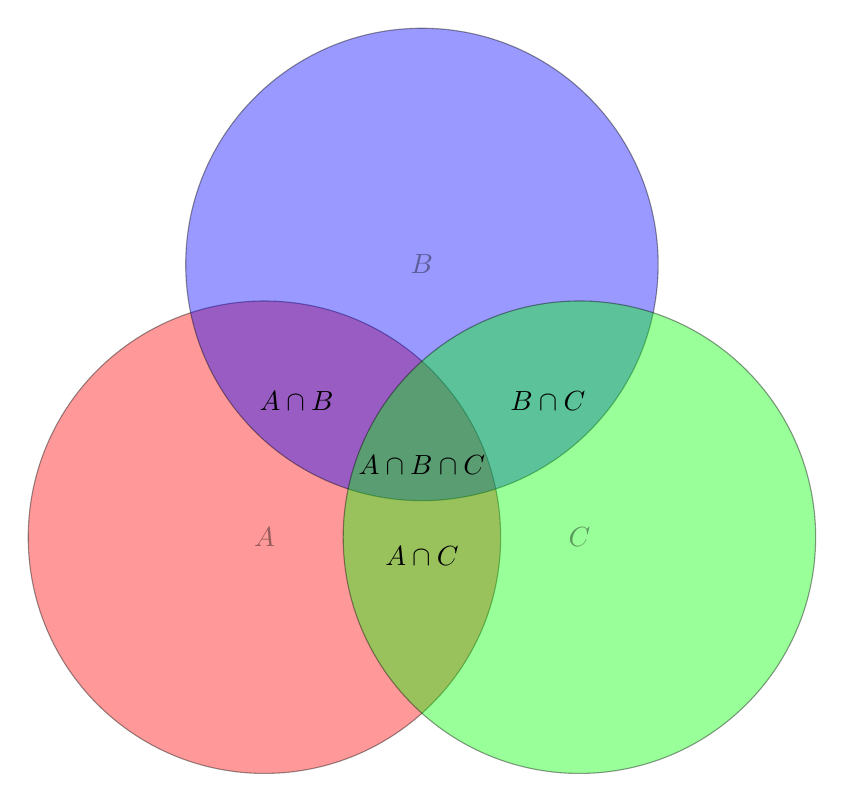
\begin{tikzpicture}
		  \tikzset{venn circle/.style={draw,circle,minimum width=6cm,fill=#1,opacity=0.4}}
		
		  \node [venn circle = red] (A) at (0,0) {$A$};
		  \node [venn circle = blue] (B) at (60:4cm) {$B$};
		  \node [venn circle = green] (C) at (0:4cm) {$C$};
		  \node[left] at (barycentric cs:A=1/2,B=1/2 ) {$A \cap B$}; 
		  \node[below] at (barycentric cs:A=1/2,C=1/2 ) {$A \cap C$};   
		  \node[right] at (barycentric cs:B=1/2,C=1/2 ) {$B \cap C$};   
		  \node[below] at (barycentric cs:A=1/3,B=1/3,C=1/3 ){$A \cap B \cap C$};
		\end{tikzpicture} 
	\end{figure}
	Nous avons donc:
	
	et les fameuses "\NewTerm{lois de De Morgan}\index{lois de De Morgan}" sous forme ensembliste (\SeeChapter{voir section de Systèmes Logiques page \pageref{de morgan theorem}}) et qui sont donn\'ees par les relations:
	
	Indiquons avant de passer à un autre sujet, qu'un nombre significatif d'adultes en emploi (souvent des cadres) en entreprise ayant oubli\'e ces notions après leur sortie de l'\'ecole obligtoire doivent les \'etudier à nouveau lorsqu'ils apprennent le language SQL (Structured Query Language) qui est le plus r\'epandu à travers le monde pour interroger les serveurs de bases de donn\'ees des entreprises au 20ème et 21ème siècles. Ils apprennent alors très en formation continue professionnelle le sch\'ema suivant pour construire leurs requêtes avec des jointures:
	\begin{figure}[H]
		\begin{center}
			\includegraphics[scale=0.33]{img/arithmetics/sql_joins.jpg}
		\end{center}	
		\caption{Jointures courantes du langage SQL bas\'e sur la th\'eorie des ensembles}
	\end{figure}

	\pagebreak
	\subsection{Fonctions et Applications}	\label{functions and applications}

	\textbf{D\'efinition (\#\mydef):} En math\'ematiques, une "\NewTerm{application}\index{application}" (ou "\NewTerm{fonction}\index{fonction}") not\'ee $f$ - en analyse fonctionnelle - ou $A$ - en algèbre lin\'eeaire - est la donn\'ee de deux ensembles, l'ensemble de d\'epart $E$ et l'ensemble d'arriv\'ee $F$ (ou d'image de $E$), et d'une relation associant à chaque \'el\'ement $x$ de l'ensemble de d\'epart un et un seul \'el\'ement de l'ensemble d'arriv\'ee, que nous appelons "\NewTerm{image de $x$ par $f$}" et que nous notons dans le domaine de l'analyse fonctionnelle par $f(x)$ ou $f(E)$ pour expliciter l'ensemble de d\'epart. Nous appelons "\NewTerm{images}\index{images}" les \'el\'ements de $f(E)$ et les \'el\'ements de $E$ sont appel\'es les "\NewTerm{ant\'ec\'edents}\index{ant\'ec\'edents}".

	Nous disons alors que $f$ est une application de $E$ dans $F$ not\'ee:
	
	(se rappeler du premier diagramme sagittal pr\'esent\'e au d\'ebut de ce chapitre), ou encore une application à arguments dans $E$ et valeurs dans $F$.

	\begin{tcolorbox}[title=Remarque,colframe=black,arc=10pt]
	Le terme "fonction" est souvent utilis\'e pour les applications à valeurs num\'eriques, r\'eelles ou complexes, c'est-à-dire lorsque l'ensemble d'arriv\'ee est $\mathbb{R}$ ou $\mathbb{C}$. Nous parlons alors de "fonction r\'eelle", ou de "fonction complexe".
	\end{tcolorbox}	
	
	\textbf{D\'efinitions (\#\mydef):}

	\begin{enumerate}
		\item[D1.] Le  "\NewTerm{graphe}\index{graphe}" (ou encore "\NewTerm{graphique}\index{graphique}" ou "repr\'esentative") d'une application $f:E \mapsto F$ est le sous-ensemble du produit cart\'esien $E \times F$ constitu\'e des couples $(x, f (x))$ pour $x$ variant dans $E$. La donn\'ee du graphe de $f$ d\'etermine son ensemble de d\'epart (par projection sur la première composante souvent not\'ee $x$) et son image (par projection sur la seconde composante souvent not\'ee $y$).
		
		\item[D2.]  Si le triplet $f(E,F,\Gamma)$ est une fonction où $E$ et $F$ sont deux ensembles et $\Gamma \subset (E \times F)$ est un graphe, $E$ et $F$ sont respectivement la source et le but de $f$. Le "\NewTerm{domaine de d\'efinition}\index{domaine de d\'efinition}" ou "\NewTerm{ensemble de d\'epart}\index{ensemble de d\'epart}" de $f$ est:
		
		
		\item[D3.] \'etant donn\'es trois ensembles $E, F$ et $G$ (non vides), toute fonction de $E \times F$ vers $G$ est appel\'ee "\NewTerm{loi de composition}\index{loi de composition}" de $E \times F$ à valeurs dans $G$.
		
		\item[D4.] Une "\NewTerm{loi de composition interne}\index{loi de composition interne}\label{internal composition law}" (ou simplement "\NewTerm{loi interne}\index{loi interne}") dans $E$ est une loi de composition de equation à valeurs dans $E$ (cas $E=F=G$). 

		\begin{tcolorbox}[title=Remarque,colframe=black,arc=10pt]
		La soustraction dans $\mathbb{N}$ n'est pas une loi de composition interne bien qu'elle fasse partie des quatre op\'erations \'el\'ementaires apprises à l'\'ecole. Par contre l'addition sur $\mathbb{N}$ en est bien une!
		\end{tcolorbox}
			
		\item[D5.] Une "\NewTerm{loi de composition externe}\index{loi de composition externe}" (ou simplement "\NewTerm{loi externe}\index{loi externe}") dans $E$ est une loi de composition de $F \times E$ à valeurs dans $E$, où $F$ est un ensemble distinct de $E$. En g\'en\'eral, $F$ est un corps, dit "\NewTerm{corps de scalaires}\index{corps de scalaires}".
	
		\begin{tcolorbox}[colframe=black,colback=white,sharp corners]
		\textbf{{\Large \ding{45}}Exemple:}\\\\
		Dans le cas d'un espace vectoriel (voir d\'efinition beaucoup plus bas) la multiplication d'un vecteur (dont les composantes se basent sur un ensemble donn\'e) par un r\'eel est une loi de composition externe.
		\end{tcolorbox}
	
		\begin{tcolorbox}[title=Remarque,colframe=black,arc=10pt]
		Une loi de composition externe à valeurs dans $E$ est aussi appel\'ee "\NewTerm{action de $F$ sur $E$}". L'ensemble $F$ est alors le domaine d'op\'erateurs. On dit aussi que $F$ opère sur $E$ (ayez en tête l'exemple des vecteurs pr\'ec\'edemment cit\'e).
		\end{tcolorbox}	
		
		\item[D5.] Nous appelons "\NewTerm{image de $f$}", et nous notons $\Ima(f)$, le sous-ensemble d\'efini par:
		
		Ainsi, "l'image" d'une application $f:E \mapsto F$ est la collection des $f(x)$ pour $x$ parcourant $E$, c'est un sous-ensemble de $F$.
		
		Et nous appelons "\NewTerm{noyau de $f$}\index{kerr}\index{noyau}\label{kerr}", et nous notons $\ker (f)$, le sous-ensemble très important en math\'ematiques d\'efini par:
		
		Selon la figure (il faut bien comprendre ce concept de noyau car nous le r\'eutiliserons de nombreuses fois pour d\'emontrer des th\'eorèmes ayant des applications pratiques importantes):
		\begin{figure}[H]
			\centering
			\includegraphics[scale=1]{img/arithmetics/ker.jpg}	
			\caption{Repr\'esentation du concept de noyau d'une fonction}
		\end{figure}
		\begin{tcolorbox}[title=Remarque,colframe=black,arc=10pt]
		\textbf{R1.} $\ker (f)$ provient de l'allemand "Kern", signifiant tout simplement "noyau". En anglais, le noyau se dit aussi "kernel", signifiant "amande" dans le civil.\\
		
		\textbf{R2.} Normalement les notations $\Ima$ et $\ker$ sont r\'eserv\'ees aux homomorphismes de groupes, d'anneaux, de corps et aux applications lin\'eaires entre espaces vectoriels ou modules etc.... (voir plus loin). Nous n'avons normalement pas l'habitude de les utiliser pour des applications quelconques entre ensembles quelconques. Mais bon...ça ne fait rien.
		\end{tcolorbox}	
	\end{enumerate}	
	\begin{tcolorbox}[colframe=black,colback=white,sharp corners]
	\textbf{{\Large \ding{45}}Exemple:}\\\\
	La fonction sinus a de son argument un noyau qui est $2\pi \mathbb{Z}$.
	\end{tcolorbox}
	Les applications peuvent avoir une quantit\'e ph\'enom\'enale de propri\'et\'es dont voici celles qui font partie des connaissances g\'en\'erales du physicien (pour plus de renseignements sur ce qu'est une fonction, voir le chapitre traitant de l'Analyse Fonctionnelle page \pageref{functional analysis}).

	Soit $f$ une application d'un ensemble $E$ à un ensemble $F$ alors nous avons les propri\'et\'es suivantes:

	\begin{enumerate}
		\item[P1.] Une application est dite "\NewTerm{surjective}\index{application surjective}\label{surjective application}" si:\\
		
		Tout \'el\'ement $y$ de $F$ est l'image par $f$ d'au moins (nous insistons sur le "au moins") un \'el\'ement de $E$. Nous disons encore que c'est une "surjection" de $E$ dans $F$. Il d\'ecoule de cette d\'efinition, qu'une application ou fonction $f:E\mapsto F$ est surjective et not\'ee:
		
		si et seulement si $F= \Ima (f)$. En d'autres termes, nous \'ecrivons aussi cette d\'efinition ainsi:
		
		\begin{figure}[H]
			\begin{center}
				\includegraphics[scale=0.75]{img/arithmetics/surjective.eps}
			\end{center}	
			\caption{Repr\'esentation d'une fonction surjective}
		\end{figure}
		
		\item[P2.] Une application est dite "\NewTerm{injective}\index{application injective}\label{injective}" si:\\
	
		Tout \'el\'ement $y$ de $F$ est l'image par $f$ d'au plus (nous insistons sur le "au plus") un seul \'el\'ement de $E$. Nous disons encore que $f$ est une injection de $E$ dans $F$. Il r\'esulte de cette d\'efinition, qu'une application $f:E\mapsto F$ est injective et not\'ee:
		
		si et seulement si les relations $x_1,x_2 \in E$  et $f(x_1)=f(x_2)$ impliquent  $x_1=x_2$ autrement dit: une application pour laquelle deux \'el\'ements distincts ont des images distinctes est dite "injective". Ou encore, une application est injective si l'une aux moins des propri\'et\'es \'equivalentes suivantes est v\'erifi\'ee:
		\begin{enumerate}
			\item[P2.1] $\forall x,y\in E^2:\;f(x)=f(y)\Rightarrow x=y$
			\item[P2.2] $\forall x,y:\;  x\neq y \Rightarrow f(x) \neq f(y)$
			\item[P2.3] $\forall y \in F$ l'\'equation en  $x$, $y=f(x)$ a au plus une solution dans $E$
		\end{enumerate}
		Tout cela s'illustrant par:
		\begin{figure}[H]
			\centering
			\includegraphics[scale=0.75]{img/arithmetics/injective.eps}	
			\caption{Repr\'esentation d'une fonction injective}
		\end{figure}
		
		\item[P3.] Une application est dite "\NewTerm{bijective}\index{application bijective}" ou "\NewTerm{application/fonction totale}\label{bijection}" si:
		
		Une application $f$ de $E$ dans $F$ est à la fois surjective et injective. Dans ce cas, nous avons que pour tout \'el\'ement $y$ de $F$, l'\'equation $y=f(x)$ admet dans $E$ une unique (ni "au plus", ni "au moins") pr\'e-image $x$ et not\'e:
		 
		Ce que nous \'ecrivons aussi plus explicitement:
		
		ce qui s'illustre par:
		\begin{figure}[H]
			\begin{center}
				\includegraphics[scale=0.75]{img/arithmetics/bijective.eps}
			\end{center}	
			\caption{Repr\'esentation d'une fonction bijective}
		\end{figure}
		Nous sommes ainsi tout naturellement amen\'es à d\'efinir une nouvelle application de $F$ dans $E$, appel\'ee "\NewTerm{fonction r\'eciproque}\index{fonction r\'eciproque}" de $f$ et not\'ee $f^{-1}$ (certaines auteurs et professeurs notent cela aussi $^rf$ parfois...), qui a tout \'el\'ement $y$ de $F$, fait correspondre l'\'el\'ement $x$ de $E$ pr\'e-image (ou aussi appel\'e "solution") unique de l'\'equation $y=f(x)$. Autrement dit:
		
		L'existence d'une application r\'eciproque implique que le graphique d'une application bijective (dans l'ensemble des r\'eels...) et celui de son application r\'eciproque sont sym\'etriques par rapport à la droite d'\'equation $y=x$.
		
		Effectivement, nous remarquons que si $y=f(x)$ est \'equivalent à $x=f^{-1}(y)$, alors ces \'equations impliquent que le point $(x, y)$ est sur le graphique de $f$ si et seulement si le point $(y, x)$ est sur le graphique de $f^{-1}$.
	
	Comme vous pouvez le voir par exemple dans la figure ci-dessous avec la fonction sinus (\SeeChapter{voir section de Trigonom\'etrie page \pageref{trigonometry}}):
	
	\begin{figure}[H]
		\begin{center}
			\includegraphics[scale=2]{img/arithmetics/bijective_example.jpg}
		\end{center}	
		\caption{Exemple de fonction bijective}
	\end{figure}

	\begin{tcolorbox}[colframe=black,colback=white,sharp corners]
	\textbf{{\Large \ding{45}}Exemple:}\\\\
	Prenons le cas d'une station de vacances où un groupe de touristes doit être log\'e dans un hôtel. Chaque façon de r\'epartir ces touristes dans les chambres de l'hôtel peut être repr\'esent\'ee par une application de l'ensemble des touristes vers l'ensemble des chambres (à chaque touriste est associ\'ee une chambre).
	\begin{itemize}
		\item Les touristes souhaitent que l'application soit injective, c'est-à-dire que chacun d'entre eux ait une chambre individuelle. Cela n'est possible que si le nombre de touristes ne d\'epasse pas le nombre de chambres.
		
		\item  L'hôtelier souhaite que l'application soit surjective, c'est-à-dire que chaque chambre soit occup\'ee. Cela n'est possible que s'il y a au moins autant de touristes que de chambres.
		
		\item S'il est possible de r\'epartir les touristes de telle sorte qu'il y en ait un seul par chambre, et que toutes les chambres soient occup\'ees: l'application sera alors à la fois injective et surjective nous dirons qu'elle est bijective.
	\end{itemize}
	\end{tcolorbox}
		
		\begin{tcolorbox}[title=Remarques,colframe=black,arc=10pt]
		\textbf{R1.}  Il vient des d\'efinitions ci-dessus qu'une application f est bijective (ou "biunivoque") dans l'ensemble des r\'eels si et seulement si toute droite horizontale coupe la repr\'esentation graphique de la fonction en un seul point. Nous sommes donc amen\'es à faire la seconde remarque suivante:\\
	
		\textbf{R2.} Une application qui v\'erifie le test de la droite horizontale est continument croissante ou d\'ecroissante en tout point de son domaine de d\'efinition.
		\end{tcolorbox}
		
		\item[P4.] Une application est dite "\NewTerm{fonction compos\'ee}\index{fonction compos\'ee}" ou "\NewTerm{fonction composite}" si:
		
		Soit $\varphi$ une application de $E$ dans $F$ et $\psi$ une fonction de $F$ dans $G$. L'application qui associe à chaque \'el\'ement $x$ de l'ensemble de $E$, un \'el\'ement $\psi(\varphi(x))$ de $G$ s'appelle "\NewTerm{application compos\'ee}\index{application compos\'ee}" de $\varphi$ et de $\psi$ et se note:
		
		où symbole "$\circ$" est appel\'e "\NewTerm{rond}\index{rond}" (à ne pas confondre avec la notation du produit scalaire que nous verrons dans la section de Calcul Vectoriel!). Donc, la relation pr\'ec\'edente s'\'ecrit "psi rond phi" mais se lit "phi rond psi"... Ainsi:
		
		Soit, de plus,  $\chi$ une application (pas une fonction!) de $G$ dans $H$. Nous v\'erifions aussitôt que l'op\'eration de composition est associative pour les applications (pous plus de d\'etails voir la section d'Algèbre Lin\'eaire page \pageref{non-commutativity matrices}):
		
		Cela nous permet d'omettre les parenthèses et d'\'ecrire plus simplement:
		
		Dans le cas particulier où $\varphi$ serait une application de $E$ dans $E$, nous notons $\varphi^k$ l'application compos\'ee $\varphi \circ \varphi \circ ... \circ \varphi$ ($k$ fois).
	\end{enumerate}
	
	Ce qui est important dans ce que nous venons de voir dans ce chapitre, c'est que toutes les propri\'et\'es d\'efinies et \'enonc\'ees ci-dessus sont applicables aux ensembles de nombres.

	Voyons en un exemple très concret et très puissant:


	\subsubsection{Th\'eorème de Cantor-Bernstein}
	\begin{tcolorbox}[colback=red!5,borderline={1mm}{2mm}{red!5},arc=0mm,boxrule=0pt]
	\bcbombe Attention! Ce th\'eorème, dont le r\'esultat peut sembler \'evident, n'est pas forc\'ement simple à aborder (son formalisme math\'ematique n'est pas très esth\'etique...). Nous vous conseillons de lire très lentement et de vous imaginer les diagrammes sagittaux dans la tête lors de la d\'emonstration.
	\end{tcolorbox}
	
	Voici l'hypothèse à d\'emontrer:
	\begin{theorem}
	Soient $X$ et $Y$ deux ensembles. S'il existe une injection (voir la d\'efinition d'une fonction injective ci-dessus) de $X$ vers $Y$ et une autre de $Y$ vers $X$, alors les deux ensembles sont en bijection (voir la d\'efinition d'une fonction bijective ci-dessus). Il s'agit donc aussi d'une relation antisym\'etrique!
	
	Ce qui s'illustre par:
	\begin{figure}[H]
		\begin{center}
			\includegraphics[scale=0.75]{img/arithmetics/cantor_bernstein.jpg}
		\end{center}	
		\caption{Repr\'esentation d'une relation antisym\'etrique}
	\end{figure}
	\end{theorem}
	Formellement ce th\'eorème est parfois \'ecrit:
	
	ou plus techniquement:
	
	Pour la d\'emonstration, nous avons besoin en toute rigueur de d\'emontrer au pr\'ealable un lemme (\'evident intuitivement mais pas formellement...) dont l'\'enonc\'e est le suivant:

	\begin{lemma}
	Soient $X, Y, Z$ trois ensembles tels que $X \subseteq Z \subseteq Y$. Si $X$ et $Y$ sont en bijection à travers une fonction $f$, alors $X$ et $Z$ sont en bijection à travers une fonction $g$.

	Techniquement, nous \'ecrivons ceci:
	
	
	Un exemple d'application de ce lemme est l'ensemble des nombres naturels $\mathbb{N}$ et des nombres rationnels $\mathbb{Q}$ qui sont en bijection. Dès lors, l'ensemble des entiers relatifs est en bijection avec l'ensemble des nombres naturels puisque $\mathbb{N} \subseteq \mathbb{Z} \subseteq \mathbb{Q}$.
	\end{lemma}

	\begin{dem}
	D'abord, au niveau formel, cr\'eons une fonction $f$ de $Y$ à $X$ telle quelle soit bijective:
	
	Nous avons besoin pour la suite d'un ensemble $A$ qui sera d\'efini par l'union des images des fonctions des fonctions $f$ (du genre $f(f(f\ldots)))$ et consturire un tel outil est là où r\'eside l'astuce!) des pr\'e-images de l'ensemble $Z$ (rappelez-vous que $Z \subseteq Y$) dont nous excluons les \'el\'ements de $X$ (ce que nous noterons pour cette d\'emonstration: $Z-X$):
	\begin{figure}[H]
		\centering
		\includegraphics[scale=1]{img/arithmetics/cantor_bernstein_construction_lemma.jpg}
	\end{figure}
	En d'autres termes (si la première forme n'est pas claire...) nous d\'efinissons l'ensemble $A$ comme \'etant l'union des images de $(Z-X)$ par les applications $f \circ f \circ ... \circ f$ Ce que nous noterons :
	
	Parce que $f:Y \mapsto X$ et que $(Z-X)\subseteq Y$ nous avons par construction $A \subseteq X$ et donc:
	
 	Remarquons que nous avons aussi:
	
	et en r\'eindexant:
	
	Nous avons alors (faire un sch\'ema de tête des diagrammes sagittaux peut aider à ce niveau-là...) quel que soit $A$:
	
	Nous pouvons d\'emontrer \'el\'egamment cette dernière relation (\'etant donn\'e que c'est aussi un des r\'esultats les plus importants!):
	
	Comme $Z$ peut être partitionn\'e (rien nous en empêche!) en les deux sous-ensembles disjoints suivants:
		
	 et sans oublier que $X \subseteq Z \subseteq Y$ et $A \subseteq X$, nous introduisons maintenant par d\'efinition la fonction $g$ (pour laquelle nous ne donne pas plus d'informations pour l'instant) telle que:
	
	tel que pour toute pr\'e-image $a$ de $g$ de la partition $((Z-X)\cup A) \subseteq Z$ nous ayons:
	
	Ce qui signifie que parce que $((Z-X)\cup A) \subseteq Z$ et $Z \subseteq Y$ nous pouvons alors appliquer (associer) la fonction bijective $f$ (rappelez-vous que $f:Y \rightarrow X$) comme \'equivalent de la fonction $g$ à tout \'el\'ement de $((Z-X)\cup A)$.

	Nous avons aussi pour tout pr\'e-image $a$ de $g$ de la partition $(X-A)$ (rappelez-vous que $A \subseteq X$):
	
	ce qui signifie que nous appliquons juste la fonction identit\'e que nous pouvons aussi associer à la fonction $g$.
	
	Donc pour r\'esumer, nous avons construit une fonction $g$ qui est alors bijective parce que ses restrictions à $((Z-X)\cup A)$ est $f$ et  $(X-A)$ is l'identiti\'e qui sont toutes deux bijectives, la première par d\'efinition, la deuxième par construction!

	Finalement il existe bien, par construction, une bijection entre $X$ et $Z$ et nous avons d\'emontr\'e le lemme que:
	
	\begin{flushright}
		$\blacksquare$  Q.E.D.
	\end{flushright}
\end{dem}

	Maintenant que nous avons prouv\'e le lemme, rappelons les hypothèses du th\'eorème de Cantor-Bernstein en utilisant le r\'esultat du lemme:
	
	Soit $\varphi$ une injection de $X$ à $Y$ et $\psi$ une injection de $Y$ à $X$ avec $X \subseteq Y$. 
	
	Nous avons alors:
	
	donc:
	
	Dès lors, nous avons jusqu'ici:
	\begin{itemize}
		\item Comme $\varphi$ est injective, alors $X$ et $\varphi(X)$ sont pas d\'efinition bijectifs (oui! effectivement, une fonction injective est par d\'efinition bijective lorsque nous r\'eduisons son ensemble image à son ensemble de pr\'e-image\footnote{mais il faut noter que cela ne fonction que pour des ensembles infinis!})
		
		\item Comme $\psi$ est injective, $\psi(\varphi(X))$ et $\varphi(X)$ est bijective.
	\end{itemize}

	Donc, du pr\'ec\'edent lemme prouv\'e, $X$ et $\psi(\varphi(X))$ sont alors aussi en bijection!
	
	En utilisant le lemme sur  $\psi(\varphi(X))$, $\psi(Y)$ et $X$ , il vient donc que $\psi(\varphi(X))$ est en bijection avec $\psi(Y)$ ce qui nous donne avec ce que nous avons vu juste pr\'ec\'edemment, que puisque $\psi(\varphi(X))$ et aussi $\varphi(X)$ sont en bijection, que  $\psi(Y)$ est en bijection avec $\varphi(X)$, et alors que $X$ et $Y$ sont reli\'es par une application bijective (ouf! c'est beau mais c'est aussi vicieux que simple) et que nous avons:
	
	Ce th\'eorème s'interprète de la manière suivante: Si nous pouvons compter une partie d'un ensemble avec la totalit\'e des \'el\'ements d'un autre ensemble, et r\'eciproquement, alors ils ont le même nombre d'\'el\'ements. Ce qui est \'evident pour des ensembles finis. Ce th\'eorème g\'en\'eralise alors cette notion pour des ensembles infinis et c'est là sa force!

	À partir de là, ce th\'eorème repr\'esente l'une des briques de base pour g\'en\'eraliser la notion de tailles d'ensembles à des ensembles infinis.
	
	\pagebreak
	\subsection{Structures}\label{structures}
	L'algèbre dite "\NewTerm{algèbre moderne}\index{algèbre moderne}" commence avec la th\'eorie des structures alg\'ebriques due en partie à Carl F. Gauss et surtout à \'evariste Galois. Ces structures existent en un très grand nombre mais seulement les fondamentales nous int\'eresseront ici. Avant de les d\'etailler, voici un diagramme synoptique de ces principales structures et de leur hi\'erarchie:
	\begin{figure}[H]
		\centering
		\includegraphics[width=1.0\textwidth]{img/arithmetics/structures_common.jpg}
		\caption{Diagramme synoptique des structures alg\'ebriques courantes}
	\end{figure}
	\begin{tcolorbox}[title=Remarque,colframe=black,arc=10pt]
	Tout en haut du diagramme, la structure au nombre minimal de contraintes, en bas, un maximum. Soit, plus nous descendons, plus la structure est en quelque sorte sp\'ecialis\'ee.
	\end{tcolorbox}	
	Soit pour simplifier les \'ecritures, supposons que $\star$ et  $\circ$ repr\'esentent des lois de compositions\footnote{Cette notation g\'en\'eralis\'ee est souvent appel\'ee "\NewTerm{notation stellaire}\index{notation stellaire}".} (comme l'addition, la soustraction, la multiplication ou encore la division,...), alors:
	
	\textbf{D\'efinitions (\#\mydef):} Soit $\star$ et $\circ$ des symboles de lois internes à un ensemble $E$ (cela pourrait être l'addition et la multiplication pour prendre les cas les plus connus) alors:
	\begin{enumerate}
		\item[D1.] $\star$ est une "\NewTerm{loi commutative}\index{loi commutative}" si: 
		
		
		\item[D2.] $\star$ est une "\NewTerm{loi associative}\index{loi associative}" si:
		
		
		\item[D3.] $n$ est "\NewTerm{l'\'el\'ement neutre}\index{l'\'el\'ement neutre}\label{neutral element}" pour $\star$ si:
		
		Nous admettrons par ailleurs sans d\'emonstration (c'est intuitif) que s'il existe un \'el\'ement neutre, il est unique.
		
		\item[D4.] $a'$ est "\NewTerm{l'\'el\'ement sym\'etrique}\index{l'\'el\'ement sym\'etrique}\label{symmetrical element}" (dans le sens g\'en\'eral de l'oppos\'e par exemple pour l'addition et l'inverse pour la multiplication) de $a$ pour $\star$  si:
		
		Nous admettrons \'egalement et sans d\'emonstration que le sym\'etrique de tout \'el\'ement est unique.		
		
		\item[D5.] $\circ$ est une "\NewTerm{loi distributive}\index{loi distributive}" par rapport à $\star$ si:
		
	
		\item[D6.] $b$ est "\NewTerm{l'\'el\'ement absorbant}\index{\'el\'ement absorbant}" si pour tout $a$ et une loi $\star$ nous avons:
		
	\end{enumerate}
	\begin{tcolorbox}[title=Remarques,colframe=black,arc=10pt]
	\textbf{R1.} Si $a$ est son propre sym\'etrique par rapport à la loi $\star$, les math\'ematiciens disent que $a$ est "\NewTerm{involutif}\index{involutif}".\\

	\textbf{R2.} Si un \'el\'ement $b$ de $E$ v\'erifie:
	
	alors $b$ est dit  "\NewTerm{\'el\'ement absorbant}\index{\'el\'ement absorbant}" pour la loi $\star$.\\

	\textbf{R3.} Il faut toujours v\'erifier que les neutres et les sym\'etriques le soient "à gauche" \underline{et} "à droite". Ainsi, par exemple, dans $(\mathbb{Z},-)$, l'\'el\'ement $0$ n'est un neutre qu'à droite car $x-0=x$ mais $0-x=-x$.
	\end{tcolorbox}	
	
	\subsubsection{Magma}
	\textbf{D\'efinition (\#\mydef):} Nous d\'esignons un ensemble par le terme "\NewTerm{magma}\index{magma}" $M$, si les composants le constituant sont op\'erables par rapport à une loi interne $\star$:
	
	Il est donc important de se rappeler que si nous d\'esignons une structure alg\'ebrique par le terme "magma" tout court, cela ne signifie en aucun cas que la loi interne est commutative, associative ou même qu'elle possède un \'el\'ement neutre !
	
	\begin{tcolorbox}[title=Remarques,colframe=black,arc=10pt]
	\textbf{R1.}  Si de plus la loi interne $\star$ est commutative, nous parlons de "\NewTerm{magma commutatif}\index{magma commutatif}".\\

	\textbf{R2.} Si de plus la loi interne $\star$  est associative, nous parlons de "\NewTerm{magma associatif}\index{magma associatif}".\\

	\textbf{R3.} Si de plus la loi interne $\star$ possède un \'el\'ement neutre $n$, nous parlons de "magma unitaire associatif" ou respectivement de "magma unitaire commutatif" mais nous verrons just pluse bas que les deux ont officiellement d\'enomm\'es autrement par les sp\'ecialistes.
	\end{tcolorbox}	
	
	\textbf{D\'efinition (\#\mydef):} Dans un magma $(M,\star)$, un \'el\'ement $x$ est nomm\'e "\NewTerm{\'el\'ement r\'egulier}\index{\'el\'ement r\'egulier}" (ou "\NewTerm{\'el\'ement simplifiable}\index{\'el\'ement simplifiable}") à gauche si pour tout couple $(a,b)\in M$ nous avons:
	
	\begin{tcolorbox}[title=Remarque,colframe=black,arc=10pt]
	Nous d\'efinissons sur la même logique un \'el\'ement r\'egulier à droite.
	\end{tcolorbox}	
	Ainsi, un \'el\'ement est dit "\NewTerm{r\'egulier}" s'il est r\'egulier à droite et à gauche. Si $\star$ est commutatif (comme dans le cas d'un magma commutatif), les notions d'\'el\'ement r\'egulier à gauche ou à droite coïncident.
	
	Un magma $(M,\star)$ est donc une structure alg\'ebrique \'el\'ementaire. Il existe des structures plus subtiles (monoïdes, groupes, anneaux, champs, espace vectoriel, etc.) dans lesquelles un ensemble est dot\'e de plusieurs lois et de diff\'erentes propri\'et\'es. Nous les verrons tout de suite et les utiliserons tout au long de ce livre de manière explicite ou implicite.
	
	\pagebreak
	\subsubsection{Monoïde}\label{monoid}
	\textbf{D\'efinition (\#\mydef):} Si la loi $\star$ est associative et possède un \'el\'ement neutre nous disons alors que le "\NewTerm{magma associatif unitaire}\index{magma associatif unitaire}" est un "\NewTerm{monoïde}\index{monoïde}":
	
	\begin{tcolorbox}[title=Remarques,colframe=black,arc=10pt]
	\textbf{R1.} Si de plus la loi interne $\star$ est commutative alors nous disons alors que la structure forme un "\NewTerm{monoïde ab\'elien}\index{monoïde ab\'elien}" (ou simplement "\NewTerm{monoïde commutatif}\index{monoïde commutatif}").\\

	\textbf{R2.} Dans certains ouvrages nous trouvons aussi comme d\'efinition que le monoïde est un "\NewTerm{semi-groupe}" (avec une loi associative $\star$) muni d'un \'el\'ement neutre $n$.
	\end{tcolorbox}
	Montrons  tout de suite que l'ensemble des entiers naturels $\mathbb{N}$ est un monoïde ab\'elien totalement ordonn\'e (comme nous l'avons partiellement vu dans la section sur les Op\'erateurs \pageref{comparators}) par rapport aux lois d'addition et de multiplication:
	
	La loi d'addition "$+$" est-elle une loi interne telle que $\forall a,b \in\mathbb{N}$ nous ayons:
	
	Nous pouvons d\'emontrer que c'est bien le cas en sachant que $1$ appartient à $\mathbb{N}$ tel que:
	
	Donc  $c\in\mathbb{N}$ et l'addition est bien une loi interne (nous disons \'egalement que l'ensemble $\mathbb{N}$ est "\NewTerm{stable}\index{stable}" par rapport à l'addition) et en même temps associative puisque $1$ peut être additionn\'e à lui-même par d\'efinition dans n'importe quel ordre sans que le r\'esultat en soit alt\'er\'e. Si vous vous rappelez que la multiplication est une loi qui se construit sur l'addition (\SeeChapter{voir la section Op\'erateurs page \pageref{multiplication}}), alors la loi de multiplication $\times$ est aussi une loi interne et associative !
	
	Nous admettrons à partir d'ici qu'il est trivial que la loi d'addition $+$ est \'egalement commutative et que le z\'ero "$0$" en est l'\'el\'ement neutre ($n$) à droite. Ainsi, la loi de multiplication est elle aussi commutative et il est trivial que "$1$" en est l'\'el\'ement neutre ($n$).

	Par ailleurs, pour parler d\'ejà de quelque chose qui n'est pas directement en relation avec le monoïde... mais qui nous sera utile un peu plus loin, existe-t-il en restant dans la lign\'ee de l'exemple pr\'ec\'edent pour la loi d'addition $+$ un sym\'etrique $\exists c$ tel que $\forall a,b\in\mathbb{N}$ nous ayons:
	
	avec $c\in\mathbb{N}$?
	
	Il est assez trivial que pour que cette \'egalit\'e soit satisfaite nous ayons:
	
	soit:
	
	or les nombres n\'egatifs n'existent pas dans $\mathbb{N}$. Ce qui nous amène aussi à la conclusion que la loi d'addition $+$ n'a pas de sym\'etrique dans $\mathbb{N}$ et que la loi de soustraction $-$ n'existe pas dans $\mathbb{N}$ (la soustraction \'etant rigoureusement l'addition d'un nombre n\'egatif!).
	
	De même, car cela va aussi nous être utile un peu plus loin, existe-t-il  pour la loi de multiplication $\times$ un sym\'etrique $a'$ tel que $\forall a\in\mathbb{N}$ nous ayons:
	
	avec $a'\in\mathbb{N}$?
	
	D'abord il est \'evident que:
	
	Mais except\'e pour $a=1$, le quotient $1/a$ n'existe pas dans $\mathbb{N}$. Donc nous devons conclure qu'il n'existe pas pour tout \'el\'ement de $\mathbb{N}$ de sym\'etriques pour la loi de multiplication et ainsi que la loi de division n'existe pas dans $\mathbb{N}$ et que la loi de multiplication ne forme pas un monoïde dans cet ensemble.

	Synthèse:
	\begin{table}[H]
		\centering
		\begin{tabular}{|
		>{\columncolor[HTML]{9B9B9B}}l |c|c|c|c|}
		\hline
		\multicolumn{1}{|c|}{\cellcolor[HTML]{9B9B9B}$\pmb{\mathbb{N}}$} & \cellcolor[HTML]{9B9B9B}$\pmb{(+)}$ & \cellcolor[HTML]{9B9B9B}$\pmb{(-)}$ & \cellcolor[HTML]{9B9B9B}$\pmb{\times}$ & \cellcolor[HTML]{9B9B9B}$\pmb{/}$ \\ \hline
		\textbf{Loi interne} & oui &  & oui &  \\ \cline{1-2} \cline{4-4}
		\textbf{Commutative} & oui &  & oui &  \\ \cline{1-2} \cline{4-4}
		\textbf{\'El\'ement neutre} & oui ($0$) &  & oui ($1$) &  \\ \cline{1-2} \cline{4-4}
		\textbf{\'El\'ement absorbant} & non &  & oui ($0$) &  \\ \cline{1-2} \cline{4-4}
		\textbf{Sym\'etrique} & non & \multirow{-5}{*}{non} & non & \multirow{-5}{*}{non} \\ \hline
		\end{tabular}
		\caption{Lois et leurs propri\'et\'es dans l'ensemble des entiers naturels $\mathbb{N}$}
	\end{table}
	Nous avons par exemple les propri\'et\'es suivantes relativement à l'ensemble des entiers naturels $\mathbb{N}$ et au concept de monoïde:
	\begin{enumerate}
		\item[P1.] $(\mathbb{N},\le,\ge)$ est totalement ordonn\'e (attention cette notation est un peu abusive! il suffit qu'il y ait juste une des deux relations d'ordre $\mathcal{R}$ pour que l'ensemble soit totalement ordonn\'e).
		
		\item[P2.] $(\mathbb{N},+)$ et $(\mathbb{N},\times)$ sont des monoïdes ab\'eliens.
		
		\item[P3.] L'\'el\'ement z\'ero "$0$" est l'\'el\'ement absorbant pour le monoïde $(\mathbb{N},\times)$.
		
		\item[P4.] Les lois de soustraction $-$ et division $/$ n'existent pas dans l'ensemble $\mathbb{N}$.
		
		\item[P5.] $\mathbb{N}$ est un monoïde ab\'elien totalement ordonn\'e par rapport aux lois d'addition et de multiplication (attention la notation suivante est abusive car le monoïde n'est compos\'e que d'une seule loi interne et d'une relation d'ordre $\mathcal{R}$ ce qui donnerait au total $4$ monoïdes):
		
	\end{enumerate}
	\begin{tcolorbox}[title=Remarques,colframe=black,arc=10pt]
	\textbf{R1.} Il est rare d'utiliser les monoïdes dansla pratique du physicien et de l'ing\'enieur. Effectivement, souvent, lorsque nous nous trouvons face à une structure trop pauvre pour pouvoir vraiment discuter, nous la prolongeons vers quelque chose de plus riche, comme un groupe, ou un anneau (voir plus loin) tel que l'ensemble des entiers relatifs $\mathbb{Q}$ ou les nombres r\'eels $\mathbb{R}$ (au moins...).\\

	\textbf{R2.} Dire qu'une structure alg\'ebrique est totalement ordonn\'ee par rapport à certaines lois signifie que soit $\star$ une loi, et $\mathcal{R}$ une relation d'ordre et $a$, $b$, $c$, $d$ quatre \'el\'ements de la structure int\'eress\'ee, alors si $a\;\mathcal{R}\;b$ et $c\;\mathcal{R}\;d$ implique $(a\star c)\mathcal{R}(b\star d)$. Nous notons alors cette structure $(S,\star, \mathcal{R})$ ou simplement $(S, \mathcal{R})$ et en indiquant la (ou les) loi concern\'ee.
	\end{tcolorbox}	
	
	\subsubsection{Groupes}\label{groups}
	\textbf{D\'efinition (\#\mydef):} Nous d\'esignons un ensemble par le terme "\NewTerm{groupe}\index{groupe}", si les composants le constituant satisfont aux trois conditions de ce que nous nommons la "\NewTerm{loi interne de groupe}\label{loi interne de groupe}", d\'efinie ci-dessous:
	
	Dans ce cas, la loi de compositions interne $\star$ sera souvent (mais pas exclusivement!) not\'ee "$+$" et appel\'ee "\NewTerm{l'addition}\index{l'addition}, le neutre $e$ not\'e "$0$" et le sym\'etrique de $x$ not\'e "$-x$".

	Insistons sur le fait que la structure de groupe est probablement une des plus importantes dans la pratique de l'ing\'enieur et de la physique moderne en g\'en\'eral. Raison pour laquelle il convient d'y porter une attention toute particulière (\SeeChapter{voir la section d'Algèbre Ensembliste page \pageref{groups}})!

	Si de plus, la loi interne $\star$ est \'egalement commutative, nous disons alors que le groupe est un "\NewTerm{groupe ab\'elien}\index{groupe ab\'elien}\label{abelian group}" ou simplement "\NewTerm{groupe commutatif}\index{groupe commutatif}".

	S'il existe dans $G$ au moins un \'el\'ement $a$ tel que tout \'el\'ement de $G$ est une puissance de $a$ ou du sym\'etrique $a'$ de $a$, nous disons que $(G,\star)$ est un "\NewTerm{groupe cyclique de g\'en\'erateur a}\index{groupe cyclique} s'il est fini, sinon nous disons qu'il est "\NewTerm{monogène}" (nous reviendrons sur les groupes cycliques dans la section d'Algèbre Ensembliste page \pageref{cyclic groups}).
	
	Plus g\'en\'eralement un groupe $(G,\star)$ d'\'el\'ement neutre $e$, non r\'eduit uniquement à $\{e\}$ sera monogène, s'il existe un \'el\'ement $a$ de $G$ distinct de $e$ tel que $G=\left\lbrace e,a^1,a^2,a^3,\ldots,a^n,\ldots\right\rbrace$. Un tel groupe sera cyclique, s'il existe un entier $n$ non nul pour lequel $a^n=e$. Le plus petit entier non nul v\'erifiant cette \'egalit\'e est alors nomm\'e "\NewTerm{l'ordre du groupe}\index{ordre du groupe}".
	
	Montrons tout de suite que l'ensemble des entiers relatifs $\mathbb{Z}$ est un groupe ab\'elien totalement ordonn\'e (comme nous l'avons vu dans la section des Op\'erateurs  page \pageref{comparators}) par rapport aux lois d'addition $+$ et de multiplication $\times$.
	
	D'abord pour raccourcir les d\'eveloppements, il est utile de rappeler que l'ensemble $\mathbb{Z}$ est un "prolongement" de $\mathbb{N}$ par le fait que nous y avons ajout\'e tous les nombres sym\'etriques de signe n\'egatif ($\mathbb{N}\subset \mathbb{Z}$).
	
	Ainsi, en abusant toujours des notations (car normalement un groupe n'a qu'une seule loi $\star$ et une seule relation d'ordre $\mathcal{R}$ suffit à l'ordonner):
	
	forme un groupe ab\'elien totalement ordonn\'e (4 groupes au fait!) et:
	
	un monoïde ab\'elien (deux monoïdes au fait!) totalement ordonn\'e.

	Remarquons aussi que la loi de division n'existe pas pour tout \'el\'ement de l'ensemble $\mathbb{Z}$! Donc en toute g\'en\'eralit\'e nous disons qu'elle n'y existe pas!

	Synthèse:
	\begin{table}[H]
		\centering
		\begin{tabular}{|
		>{\columncolor[HTML]{9B9B9B}}l |c|c|c|c|}
		\hline
		$\pmb{\mathbb{Z}}$ & \multicolumn{1}{c|}{\cellcolor[HTML]{9B9B9B}$\pmb{(+)}$} & \multicolumn{1}{c|}{\cellcolor[HTML]{9B9B9B}$\pmb{(-)}$} & \multicolumn{1}{c|}{\cellcolor[HTML]{9B9B9B}$\pmb{(\times)}$} & \multicolumn{1}{c|}{\cellcolor[HTML]{9B9B9B}$\pmb{(/)}$} \\ \hline
		\textbf{Loi interne} & oui & oui & oui &  \\ \cline{1-4}
		\textbf{Associativit\'e} & oui & non & oui &  \\ \cline{1-4}
		\textbf{Commutativit\'e} & oui & non & oui &  \\ \cline{1-4}
		\textbf{\'El\'ement neutre} & oui ($0$) & \begin{tabular}[c]{@{}c@{}}non\\ {\footnotesize ($0$ pas neutre à gauche)}\end{tabular} & oui ($1$) &  \\ \cline{1-4}
		\textbf{\'El\'ement absorbant} & non & non & oui ($0$) &  \\ \cline{1-4}
		\textbf{Sym\'etrique} & \begin{tabular}[c]{@{}c@{}}oui\\ {\footnotesize (signe oppos\'e)}\end{tabular} & oui & non & \multirow{-6}{*}{non} \\ \hline
		\end{tabular}
		\caption{Lois et leurs propri\'et\'es dans l'ensemble des entiers relatifs $\mathbb{Z}$}
	\end{table}
	Nous avons donc les propri\'et\'es suivantes:
	\begin{enumerate}
		\item[P1.] $(\mathbb{Z},\le,\ge)$ est totalement ordonn\'e (attention à nouveau cette notation est un peu abusive! il suffit qu'il y ait juste une des deux relations d'ordre $\mathcal{R}$ pour que l'ensemble soit totalement ordonn\'e).

		\item[P2.] $(\mathbb{Z},+)$ est un groupe commutatif dont z\'ero "$0$" est l'\'el\'ement neutre.

		\item[P3.] La loi de division n'existe pas dans l'ensemble $\mathbb{Z}$.

		\item[P4.] L'ensemble $\mathbb{Z}$ est un groupe ab\'elien totalement ordonn\'e par rapport à la loi d'addition (attention la notation suivante est encore une fois abusive car le groupe est compos\'e que d'une relation d'ordre $\mathcal{R}$ ce qui donnerait au total deux groupes):
		
		L'ensemble $\mathbb{Z}$ n'est pas un groupe commutatif totalement ordonn\'e par rapport à la loi de multiplication:
		
	\end{enumerate}
	Nous voyons de suite alors que $\mathbb{Z}$ a des propri\'et\'es trop restreintes, c'est la raison pour laquelle il est int\'eressant de le prolonger par l'ensemble des rationnels $\mathbb{Q}$  d\'efini de manière très simpliste... par (\SeeChapter{voir la section Nombres page \pageref{rational numbers}}):
	
	Ce qui signifie pour rappel que l'ensemble des rationnels $\mathbb{Q}$ est d\'efini par l'ensemble des quotients $p$ et $q$ appartenant chacun à  $\mathbb{Z}$ dont nous excluons à $q$ de prendre la valeur nulle (la notation $/q$ signifiant pour rappel l'exclusion).
	
	Et nous avons \'evidemment:
	
	Il est dès lors \'evident (sans d\'emonstration et toujours en utilisant la notation abusive d\'ejà comment\'ee maintes fois plus haut...) que  $(\mathbb{Q},\le,\ge)$ est aussi totalement ordonn\'e et aussi que $\mathbb{Q}$ est un groupe ab\'elien totalement ordonn\'e par rapport à la loi d'addition $+$ seulement:
	
	Ce qui devient int\'eressant avec $\mathbb{Q}$, c'est que la loi de multiplication $\times$ devient une loi interne et forme un groupe ab\'elien commutatif dit "groupe multiplicatif" par rapport à $\mathbb{Q}^{*}$.
	\begin{dem}
	D\'emontrons donc que le sym\'etrique existe pour la loi de multiplication $\times$ tel que:
	
	Puisque dans $\mathbb{Q}^{*}$ tout nombre peut se mettre sous la forme:
	
	avec  $p\in\mathbb{Z}$, $q\in\mathbb{Z}^{*}$.
	
	Alors puisque:
	
	Il existe donc un sym\'etrique à tout rationnel dans $\mathbb{Q}^{*}$ pour la loi de multiplication.
	\begin{flushright}
		$\blacksquare$  Q.E.D.
	\end{flushright}
	\end{dem}
	Par d\'efinition, ou par construction, la division existe dans  $\mathbb{Q}^{*}$ et est une loi interne. Mais est-elle associative telle que pour $\forall (p,q,r)\in\mathbb{Q}^{*}$ nous ayons:
	
	Au fait, la d\'emonstration est assez triviale si nous nous rappelons que la division se d\'efinit à partir de la loi de multiplication par l'inverse et que cette dernière loi est (elle!) associative. Ainsi, il vient:
	
	Donc la loi de division n'est pas associative dans $\mathbb{Q}^{*}$.
	
	Nous pouvons aussi nous demander si la loi de division ($/$) est cependant commutative tel que la relation:
	
	soit valable pour $\forall (a,b)\in\mathbb{Q}^{*}$.
	
	Nous voyons très bien que cela n'est pas le cas puisque nous pouvons \'ecrire cette dernière relation sous la forme:
	
	Pour r\'esumer:
	\begin{table}[H]
		\centering
		\begin{tabular}{|
		>{\columncolor[HTML]{9B9B9B}}l |c|c|c|c|}
		\hline
		$\pmb{\mathbb{Q}}$ & \multicolumn{1}{c|}{\cellcolor[HTML]{9B9B9B}$\pmb{(+)}$} & \multicolumn{1}{c|}{\cellcolor[HTML]{9B9B9B}$\pmb{(-)}$} & \multicolumn{1}{c|}{\cellcolor[HTML]{9B9B9B}$\pmb{(\times)}$} & \multicolumn{1}{c|}{\cellcolor[HTML]{9B9B9B}$\pmb{(/)}$} \\ \hline
		\textbf{Loi interne} & oui & oui & oui & oui \\ \hline
		\textbf{Associativit\'e} & oui & non & oui & non \\ \hline
		\textbf{Commutativit\'e} & oui & non & oui & non \\ \hline
		\textbf{\'el\'ement neutre} & oui ($0$) & \begin{tabular}[c]{@{}c@{}}non\\ {\footnotesize ($0$ pas neutre à gauche)}\end{tabular} & oui ($1$) & \begin{tabular}[c]{@{}c@{}}oui\\ {\footnotesize ($1$ neutre à droite)}\end{tabular} \\ \hline
		\textbf{\'el\'ement absorbant} & non & non & oui ($0$) & \begin{tabular}[c]{@{}c@{}}oui\\ {\footnotesize ($0$ au num\'erateur)}\end{tabular} \\ \hline
		\textbf{Sym\'etrique} & \begin{tabular}[c]{@{}c@{}}oui\\ {\footnotesize (signe oppos\'e)}\end{tabular} & \begin{tabular}[c]{@{}c@{}}oui\\ {\footnotesize (signe oppos\'e)}\end{tabular} & \begin{tabular}[c]{@{}c@{}}non\\ {\footnotesize (except\'e dans $\mathbb{Q}^{*}$)}\end{tabular} & non \\ \hline
		\end{tabular}
		\caption{Lois et leurs propri\'et\'es dans l'ensemble des rationnels $\mathbb{Q}$}
	\end{table}
	Nous avons donc les propri\'et\'es suivantes:
	\begin{enumerate}
		\item[P1.] $(\mathbb{Q},\le,\ge)$ est totalement ordonn\'e
	
		\item[P2.] $(\mathbb{Q},+),(\mathbb{Q}^{*},\times)$ sont ind\'ependamment des groupes ab\'eliens totalement ordonn\'es
	
		\item[P3.] Z\'ero  "$0$" est l'\'el\'ement absorbant par rapport au  groupe $(\mathbb{Q}^{*},\times)$
	
		\item[P4.] L'ensemble $\mathbb{Q}$ est un groupe ab\'elien totalement ordonn\'e par rapport aux lois d'addition et de multiplication que nous notons:
		
	\end{enumerate}
	Les mêmes propri\'et\'es sont applicables à $\mathbb{R}$ et à $\mathbb{C}$ mais à la diff\'erence que ce dernier n'est pas ordonnable.
	
	Cependant, il peut être compr\'ehensible que pour $\mathbb{C}$ vous soyez sceptiques. D\'eveloppons donc tout cela:
	
	Nous devons nous assurer que la somme "$+$", la diff\'erence "$-$", le produit "$\times$" et le quotient "$/$" de deux nombres de la forme  $x+\mathrm{i}y$ donne quelque chose d'encore de cette forme (c'est-à-dire une application du type $\mathbb{C}\mapsto \mathbb{C}$).

	Additionnons les nombres $a+\mathrm{i}b$ et  $c+\mathrm{i}d$ où $a$, $b$, $c$ et $d$ sont des r\'eels:
	
	Donc l'addition est bien une loi interne commutative et associative pour laquelle il existe un \'el\'ement neutre et sym\'etrique dans l'ensemble des complexes $\mathbb{C}$.
	
	Soustrayons les nombres $a+\mathrm{i}b$ et $c+\mathrm{i}d$ où  $a$, $b$, $c$ et $d$ sont ici encore, des r\'eels:
	
	Donc la soustraction est une op\'eration interne; elle n'est ni commutative, ni associative elle n'a pas d'\'el\'ement neutre à gauche et pas de sym\'etrique.
	
	Multiplions maintenant les nombres $a+\mathrm{i}b$ et $c+\mathrm{i}b$ où $a$, $b$, $c$ et $d$ là toujours, sont des r\'eels. Pour parvenir à nos fins, nous emploierons la distributivit\'e de la multiplication par rapport à l'addition:
	
	Donc la loi de multiplication est bien une op\'eration interne commutative, associative et distributive (!) pour laquelle il existe un \'el\'ement neutre et sym\'etrique dans $\mathbb{C}^{*}$ (voir ci-après).
	
	Une division est avant tout une multiplication par l'inverse. Prouver qu'il existe un inverse c'est prouver qu'il existe un sym\'etrique pour la multiplication. Inversons donc le nombre $x+\mathrm{i}y$ où  $x$ et $y$ sont des r\'eels (diff\'erents de z\'ero):
	
	Donc l'inverse d'un nombre complexe est bien une op\'eration interne non associative et non commutative pour laquelle il existe un \'el\'ement neutre, et elle est sym\'etrique. Il en est de même pour la division, qui correspond au produit par l'inverse d'un nombre complexe.
	
	
	Voyons un exemple de groupe cyclique (nous approfondirons le sujet dans la section d'Algèbre Ensemble à la page \pageref{cyclic groups}): Dans  $\mathbb{C}$, consid\'erons $G = \{1, \mathrm{i}, -1, -\mathrm{i}\}$ muni de la multiplication usuelle des nombres complexes. Alors $(G,\times)$ est \'evidemment un groupe ab\'elien. Un tel groupe est aussi monogène car engendr\'e par les puissances d'un de ses \'el\'ements: $\mathrm{i}$ (ou bien $-\mathrm{i}$). Ce groupe monogène \'etant fini, il s'agit alors d'un "cyclic group\index{cyclic group}".
	
	\subsubsection{Anneaux}\label{ring}
	L'anneau est le coeur de l'algèbre commutative qui est la structure alg\'ebrique correspondant aux concepts coll\'egiens d'addition, de soustraction, et de multiplication.
	
	\textbf{D\'efinition (\#\mydef):}  Un groupe commutatif (ou "groupe ab\'elien") $A$ est un "\NewTerm{anneau}\index{anneau}" s'il est muni d'une seconde loi de composition interne v\'erifiant les propri\'et\'es suivante:
	
	Comme nous le savons d\'ejà, l'\'el\'ement neutre de la première loi de composition interne "$+$" est not\'e "$0$" et appel\'e le "z\'ero" de l'anneau. La deuxième loi interne est souvent not\'ee par un point à mi-hauteur $\cdot$ (ou par une crois $\times$ dans les petites classes) et appel\'ee la "multiplication".
	
	\begin{tcolorbox}[title=Remarques,colframe=black,arc=10pt]
	\textbf{R1.} Si de plus, la deuxième loi interne de composition "$\times$" est \'egalement commutative, l'anneau est dit "\NewTerm{anneau commutatif}\index{anneau commutatif}\label{communtative ring}". Nous rencontrons aussi des anneaux non-commutatifs dans lesquels la relation de commutativit\'e n'est pas impos\'ee ou ne s'impose pas et alors nous devons parfois l'imposer, il faut alors renforcer la propri\'et\'e de l'\'el\'ement neutre de cette deuxième loi en imposant à "$1$" d'être un \'el\'ement neutre à la fois à droite et à gauche tel que: $1a=a1=a$ (un exemple d'anneau non-commutatif est fourni par l'ensemble des matrices carr\'ees $n\times n$ à coefficients dans un anneau $A$, par exemple $M_n(\mathbb{R})$ comme nous le verrons dans la section d'Algèbre Lin\'eaire page \pageref{non-commutativity matrices}).\\

	\textbf{R2.} Si de plus, il existe dans $A$ un \'el\'ement neutre pour la deuxième loi de composition interne "$\times$", et que cet \'el\'ement neutre est l'unit\'e "$1$" nous disons alors que l'anneau est un "\NewTerm{anneau unitaire}\index{anneau unitaire}" et $1$ est appel\'e "\NewTerm{unit\'e de l'anneau}". Si l'anneau est commutatif et possède un \'el\'ement neutre pour la deuxième loi de composition interne alors nous parlons "\NewTerm{d'anneau commutatif unitaire}\index{anneau commutatif unitaire}".\\
	
	\textbf{R3.}  Si $a\times b=0\Rightarrow (a=0\text{ ou } b=0)$, quels que soient les \'el\'ements $a$, $b$ de $A$, l'anneau est dit "\NewTerm{anneau intègre}\index{anneau intègre}" ou "\NewTerm{anneau sans diviseurs de z\'ero}" (dans le cas contraire il est bien \'evidemment un "\NewTerm{anneau non-intègre}").\\
	
	\textbf{R4.} Un "\NewTerm{anneau factoriel}\index{anneau factoriel}" est un anneau commutatif unitaire et intègre dans lequel le th\'eorème fondamental de l'arithm\'etique est v\'erifi\'e (\SeeChapter{voir Sectoin Th\'eorie des Nombres page \pageref{fundamental theorem of arithmetic}}).
	\end{tcolorbox}	

	\textbf{D\'efinitions (\#\mydef):}
	\begin{enumerate}
		\item[D1.] Un \'el\'ement  $a$ d'un anneau $A$ est un "\'el\'ement unit\'e" s'il existe  $b\in A$ tel que $ab=ba=1$. Si un tel $b$ existe il est unique (nous en avons vu un exemple lors de notre \'etude des classes de congruence dans la section de Th\'eorie des Nombres page \pageref{congruence}).

		\item[D2.] Un \'el\'ement $a$ d'un anneau $A$ s'appelle un "\NewTerm{diviseur nul à gauche} \index{diviseur nul à gauche}" s'il existe $x\neq 0$ tel que $ ax = 0 $. De même, un \'el\'ement $a$ d'un anneau est nomm\'e "\NewTerm{diviseur nul à droite}\index{diviseur nul à droite}" s'il existe $ y \neq 0 $ tel que $ ya = 0 $. Un \'el\'ement $a$ qui est à la fois un diviseur gauche ET un diviseur \'egal à z\'ero s'appelle un "\NewTerm{diviseur nul bilat\'eral}\footnote{Si l'anneau est commutatif, les diviseurs nuls à gauche et à droite sont \'evidemment les mêmes.}\index{diviseur nul bilat\'eral}".
	\end{enumerate}
	\begin{tcolorbox}[colframe=black,colback=white,sharp corners]
	\textbf{{\Large \ding{45}}Exemples:}\\\\
	E1. Le seul diviseur nul de l'anneau des entiers relatifs $\mathbb{Z}$ est $0$.\\
	
	E2. Dans l'anneau des matrices carr\'ees $2\times 2$ (sur tout anneau non-nul)nous pouvons trouver un $a$ et un $x$ non-nul comme suit:
	
	Dans ce dernier exemple, il est difficile de choisir laquelle des matrices le "diviseur null", c’est pourquoi nous pouvons trouver dans certains manuels scolaires que $a$ ET $x$ sont consid\'er\'es tous deux comme des "diviseurs nuls"...
	\end{tcolorbox} 
	\begin{tcolorbox}[title=Remarques,colframe=black,arc=10pt]
	\textbf{R1.}  Il devrait être clair à ce niveau de lecture qu'un anneau est intègre si et seulement si il ne possède aucun diviseur de z\'ero.\\

	\textbf{R2.} Les notions d'unit\'e et de diviseurs de z\'ero sont incompatibles mais un \'el\'ement d'un anneau peut être ni l'un ni l'autre. C'est le cas, par exemple, de tous les entiers  diff\'erents de $\{0,-1,1\}$ dans $\mathbb{Z}$. Ce ne sont ni des unit\'es, ni des diviseurs de z\'ero! Nous les appelons des "\NewTerm{\'el\'ements r\'eguliers}\index{\'el\'ements r\'eguliers}".
	\end{tcolorbox}
	Nous verrons un exemple important d'anneaux dans le cadre de notre \'etude des polynômes (\SeeChapter{voir section de Calcul Alg\'ebrique page \pageref{polynomial ring}}) mais nous en avons d\'ejà vu de très importants lors de notre \'etude des classes de congruence dans la section de Th\'eorie des Nombres page \pageref{congruence}.
	
	Voyons quelques exemples d'anneaux! Lors de notre \'etude des groupes plus haut, nous avons trouv\'e que les structures:
	
	sont tous les quatre des groupes ab\'eliens et les trois premiers sont en plus totalement ordonn\'es.
	
	La loi de division n'\'etant en aucun cas associative, nous pouvons nous restreindre à \'etudier pour chacun des groupes pr\'ecit\'es, le couple de lois: "$+$" et "$\times$".

	Ainsi, il vient très vite que:
	
	constituent des anneaux commutatifs unitaires et intègres.
	
	\begin{tcolorbox}[title=Remarque,colframe=black,arc=10pt]
	Nous consid\'ererons comme \'evident, à ce niveau du discours, que le lecteur aura remarqu\'e que est $\mathbb{Z}$ un "sous-anneau" de $\mathbb{Q}$ dans le sens où les op\'erations d\'efinies sont internes à chacun des ensembles et que les \'el\'ements neutres et identit\'e sont identiques et qu'il existe pour chaque \'el\'ement de ces ensembles un oppos\'e qui est dans le même ensemble. Nous allons approfondir le concept de sous-anneau un peu plus loin.
	\end{tcolorbox}	
	Soit $A$ un anneau. Nous avons les propri\'et\'es suivantes:
	\begin{enumerate}
		\item[P1.] $a+b=a+c\Rightarrow (b=c)\qquad \forall a,b,c\in A$
		\begin{dem}
		Ceci d\'ecoule de la d\'efinition D4 vue au d\'ebut de la partie concernant les structures alg\'ebriques (chaque \'el\'ement a un oppos\'e / sym\'etrique). En effet, nous pouvons ajouter à:
		
		l'\'el\'ement $-a$. Nous obtenons alors:
		
		par l'existence de l'oppos\'e cela donne:
		
		d'où:
		
		\begin{flushright}
			$\blacksquare$  Q.E.D.
		\end{flushright}
		\end{dem}

		\item[P2.] $0\cdot a=0\qquad \forall a\in A$
		\begin{dem}
		Cette propri\'et\'e d\'ecoule des d\'efinitions D3 (existence de l'\'el\'ement neutre), D4 (existence de l'oppos\'e/sym\'etrique), D5 (distributivit\'e par rapport à l'autre loi) ainsi que de la propri\'et\'e P1 ci-dessus. En effet, nous avons:
		
		Nous avons donc:
		
	 	La propri\'et\'e P1 ci-dessus permet de conclure que:
		
		(nous pourrions discuter de la pertinence de ce genre de d\'emonstration...).
		\begin{flushright}
		$\blacksquare$  Q.E.D.
		\end{flushright}
		\end{dem}

		\item[P3.] $(-1)\cdot a=-a\qquad \forall a\in A$
		\begin{dem}
		Cette propri\'et\'e se d\'emontre à l'aide de P2. Nous avons:
		
		en ajoutant $-a$ à cette dernière \'egalit\'e, nous avons:
		
			\begin{flushright}
			$\blacksquare$  Q.E.D.
		\end{flushright}
		\end{dem}
	\end{enumerate}
	
	\paragraph{Sous-anneau}\mbox{}\\\\
	\textbf{D\'efinitions (\#\mydef):} Soit $A$ un anneau et  $S\subset A$ un sous-ensemble de $A$. Nous disons que $S$ est un "\NewTerm{sous-anneau}\index{sous-anneau}" de $A$ si:
	\begin{enumerate}
		\item[P1.] $n\in S$ (l'\'el\'ement neutre de $A$ est aussi celui de $S$)

		\item[P2.] $a\in S \Rightarrow -a\in S$

		\item[P3.] $(a,b)\in S\Rightarrow a+b\in S$

		\item[P4.] $(a,b)\in S\Rightarrow a\cdot b\in S$
	\end{enumerate}
	\begin{tcolorbox}[colframe=black,colback=white,sharp corners]
	\textbf{{\Large \ding{45}}Exemple:}\\\\
	L'anneau $\mathbb{Z}$ est un sous-anneau de $\mathbb{Q}$ et $\mathbb{R}$
	\end{tcolorbox}
	
	\subsubsection{Corps}
	\textbf{D\'efinition (\#\mydef):} Nous d\'esignons un ensemble de nombres par le terme "\NewTerm{corps}\index{corps (ensemble)}\label{field (set)}" si:
	
	Donc un corps est un anneau non nul dans lequel tout \'el\'ement non nul est inversible ou en d'autres termes: un anneau dont tous les \'el\'ements non nuls sont des unit\'es est un corps.
	\begin{tcolorbox}[title=Remarques,colframe=black,arc=10pt]
	\textbf{R1.} Si la loi interne $\times$ est \'egalement commutative, le corps est dit "\NewTerm{corps commutatif}\index{corps commutatif}".\\

	\textbf{R2.} Les quaternions (\SeeChapter{voir section Nombres page \pageref{quaternions}}) forment par exemple un corps non commutatif pour l'addition et la multiplication.
	\end{tcolorbox}
	Voyons des exemples de corps parmi les anneaux unitaires suivant:
	
	Il nous faut d'abord d\'eterminer lesquels ne constituent pas des groupes par rapport à la loi interne de multiplication "$\times$".
	
	Comme nous l'avons d\'ejà vu dans notre \'etude des groupes pr\'ec\'edemment, il est \'evident qu'il nous faut \'eliminer $(\mathbb{Z},+,\times)$ à cause de l'existence des inverses qui n'est pas assur\'ee dans cet ensemble.

	Ainsi, les corps fondamentaux de l'arithm\'etique sont:
	
	et puisque la loi de multiplication "$\times$" est commutative dans ces ensembles, nous pouvons affirmer que ces corps sont \'egalement des corps commutatifs.

	Nous avons souvent dans les petites classes le sch\'ema suivant pour le corps le plus important:
	
	Ainsi, nous appellerons "corps" un système $C$ de nombres r\'eels ou complexes $a$ tels que la somme, la diff\'erence, le produit et le quotient de deux quelconques de ces nombres $a$ appartiennent au même système $C$.
	
	Nous \'enonçons \'egalement cette propri\'et\'e de la manière suivante: les nombres d'un corps se reproduisent par les op\'erations rationnelles (addition, soustraction, multiplication, division). Ainsi, il est \'evident que le nombre z\'ero ne pourra jamais former le d\'enominateur d'un quotient et l'ensemble des entiers ne peut former un corps car la division dans l'ensemble des nombres entiers ne donne pas n\'ecessairement un r\'esultat dans ce même ensemble.
	
	\pagebreak
	\subsubsection{Espaces vectoriels}\label{vector space}
	Lorsque nous d\'efinissons un "\NewTerm{vector}" (\SeeChapter{voir section de Calcul Vectorel page \pageref{vector}}), nous faisons habituellement r\'ef\'erence à un "espace euclidien" (voir aussi la section de Calcul Vectoriel) de $n$ dimensions de $\mathbb{R}^n$. Cependant, la notion d'espace vectoriel est beaucoup beaucoup plus vaste que ce dernier qui ne repr\'esente qu'un cas particulier!
	
	\textbf{D\'efinition (\#\mydef):} Un "\NewTerm{espace vectoriel}\index{vector space}" (EV) ou "\NewTerm{$K$-espace vectoriel}" (abr\'eg\'e parfois $K$-ev) sur le corps $K$ (nous prendrons fr\'equemment pour ce corps $\mathbb{R}$ ou $\mathbb{C}$) est un ensemble $(E,+,\cdot)$ poss\'edant les propri\'et\'es suivantes:
	
	Nous avons donc deux lois de composition (en prenant les notations traditionnelles des vecteurs qui sera peut-être plus parlante et utile pour la suite...):
	\begin{enumerate}
		\item Une loi de composition interne: l'addition not\'ee "$+$" qui v\'erifie:
		\begin{enumerate}[label*=\arabic*.]
			\item Associativit\'e:
			
			
			\item Commutativit\'e: 
			
			
			\item \'el\'ement neutre:
			
			
			\item \'el\'ement oppos\'e 
			
		\end{enumerate}
		\item Une loi de composition externe: la multiplication par un scalaire, not\'ee "$\cdot$" (pour \'eviter la confusion avec le produit vectoriel que nous introduirons dans la section de Calcul Vectoriel à la page \pageref{cross product}), qui v\'erifie:
		\begin{enumerate}[label*=\arabic*.]
			\item Associativit\'e:
			
			
			\item Distributivit\'e à droite par rapport au corps $K$:  
			
			
			\item Distributivit\'e à gauche par rapport à $E$:
				
	
			\item  \'El\'ement neutre (de $K$ sur $E$):
			
		\end{enumerate}
	\end{enumerate}
	D'où $10$ propri\'et\'es au total (oui... le fait d'avoir une loi interne ou externe est une propri\'et\'e en soit!).
	
	Nous disons alors que l'espace vectoriel a une "\NewTerm{structure alg\'ebrique vectorielle}" et que ces \'el\'ements sont des "\NewTerm{vectors}", les \'el\'ements de $K$ \'etant des "scalaires" (\SeeChapter{voir section Nombres page \pageref{scalar}}).
	\begin{tcolorbox}[title=Remarques,colframe=black,arc=10pt]
	\textbf{R1.} Les op\'erations respectives s'utilisent fr\'equemment comme l'addition et la multiplication que nous connaissons d\'ejà très bien sur equation, ce qui est bien commode pour nos habitudes...\\
	
	\textbf{R2.} Dor\'enavant, pour distinguer les \'el\'ements du corps $K$ et de l'ensemble $E$, nous noterons ceux de $K$ par des lettres grecques et ceux de $E$ par des lettres latines majuscules.
	\end{tcolorbox}
	Il est inutile de d\'emontrer que ces propri\'et\'es sont respect\'ees pour $\mathbb{R}^n$ et, par cons\'equent pour $\mathbb{R}^2$. Nous pouvons cependant nous poser la question à propos de certains sous-ensembles de $\mathbb{R}^n$.
	\begin{tcolorbox}[colframe=black,colback=white,sharp corners]
	\textbf{{\Large \ding{45}}Exemples:}\\\\
	E1.  Consid\'erons la r\'egion rectangulaire de $\mathbb{R}^3$ illustr\'ee dans la figure ($a$) et en perspective dans la figure ($c$) ci-dessous:
	\begin{figure}[H]
		\begin{center}
			\includegraphics[scale=0.9]{img/arithmetics/vector_space_concept.jpg}
		\end{center}	
		\caption{Exemple du concept d'espace vectoriel}
	\end{figure}
	Ce sous-ensemble de $\mathbb{R}^2$ n'est pas un espace vectoriel car, entre autres, la propri\'et\'e d'op\'eration interne du groupe ab\'elien n'est pas satisfaite. En effet, si nous prenons deux vecteurs $\vec{v}$,$\vec{w}$ à l'int\'erieur du rectangle et que nous les additionnons $\vec{v}+\vec{w}$, il se peut que le r\'esultat sorte du rectangle. Par contre, il est facile de voir que la droite $\mathbb{R}^1$ (infinie) illustr\'ee dans la figure ($b$) respecte toutes les propri\'et\'es \'enum\'er\'ees pr\'ec\'edemment et, par cons\'equent, d\'efini un espace vectoriel. Notons bien, cependant, que cette droite se doit de passer par l'origine, sinon la propri\'et\'e d'\'el\'ement neutre du groupe ab\'elien ne serait pas respect\'ee (l'\'el\'ement neutre n'existant plus).\\
	
	E2. Un autre exemple d'un espace vectoriel est "\NewTerm{l'espace vectoriel polynomial}\index{espace vectoriel polynomial}" des polynômes de degr\'e deux ou moins not\'e  $\mathcal{P}^2$  (\SeeChapter{voir section de Calcul Alg\'ebrique page \pageref{polynomial vector}}). Par exemple, deux \'el\'ements choisis al\'eatoirement de cet espace sont:
	
	Cet ensemble respecte les propri\'et\'es d'un espace vectoriel. En effet, si nous additionnons deux polynômes de degr\'e deux ou moins, nous obtenons un autre polynôme de degr\'e deux ou moins. Nous pouvons aussi multiplier un polynôme par un scalaire sans changer l'ordre (ou degr\'e) de celui-ci, etc. Nous pouvons donc repr\'esenter un polynôme par des vecteurs dont les termes sont les coefficients du polynôme.
	\end{tcolorbox}
	Mentionnons que nous pouvons aussi former des espaces vectoriels avec des ensembles de fonctions plus g\'en\'erales que des polynômes. Il importe seulement de respecter les $10$ propri\'et\'es fondamentales d'un espace vectoriel !
	
	Ainsi d\'efini, un espace vectoriel $E$ sur $K$ est une action de $(K,\times)$ sur $(E,+)$ qui est compatible avec la loi de groupe (par extension un "automorphisme" - voir la d\'efinition plus loin - sur $(E,+)$).
	
	\textbf{D\'efinition (\#\mydef):} Soit $E$ un espace vectoriel, nous appelons "\NewTerm{sous-espace vectoriel}\index{sous-espace vectoriel}" (SEV) $F$ de $E$ un sous-ensemble de $E$ si et seulement si (notation des matheux...):
	
	ou en utilisant une autre notation (celle utilis\'ee plutôt par les physiciens):
	
	
	\subsubsection{$C$-algèbre $A$}
	\textbf{D\'efinition (\#\mydef):}  Une "\NewTerm{$C$-algèbre $A$}\index{$C$-algèbre $A$}" où $C$ est un corps commutatif (appel\'ee aussi souvent "$K$-alègbre $A$" pour "Körper" en allemand)), est un ensemble $A$ muni de deux lois de composition internes $+$ (addition) et $\times$ (produit en croix) et d'une loi externe "$\cdot$" (multiplication) à domaine d'op\'erateurs $C$ (produit par un scalaire) si et seulement si:
	
	\begin{tcolorbox}[colframe=black,colback=white,sharp corners]
	\textbf{{\Large \ding{45}}Exemples:}\\\\
	E1. Pour reprendre un exemple dans la lign\'ee de celui sur les exemples vectoriels, l'espace euclidien $\mathbb{R}^3$ muni de l'addition "$+$", de la multiplication "$\cdot$" et du produit vectoriel "$\times$" est une $\mathbb{R}$-algèbre non associative et non commutative not\'ee $(\mathbb{R}^3,\mathbb{R},+,\cdot,\times)$.\\
	
	E2.  L'ensemble $\mathbb{C}$  est une $\mathbb{R}$-algèbre (un nombre complexe pouvant être vu comme un vecteur à deux composantes selon ce que nous avons vu dans la section des Nombres page \pageref{gauss plane}).
	\end{tcolorbox}
	
	
	\pagebreak
	\subsubsection{R\'esum\'e}
	Ok ... jusqu'ici il y a eu beaucoup de d\'efinitions et de concepts. Pour r\'esumer les structures alg\'ebriques les plus importantes observ\'ees jusqu'à pr\'esent, nous avons obtenu l'autorisation de Kevin Binz de reproduire ses très belles figures visuelles qui pourraient aider le cerveau du lecteur à avoir une vue d'ensemble des concepts les plus importants vus jusqu'à pr\'esent.

	Commençons donc par introduire les diff\'erentes structures d’ensembles du point de vue où nous les construisons en ajoutant à chaque fois une nouvelle propri\'et\'e:
	\begin{table}[H]
		\centering
		\begin{tabular}{llll|l|}
		\hline
		\rowcolor[HTML]{9B9B9B} 
		\multicolumn{1}{|l|}{\cellcolor[HTML]{9B9B9B}\textbf{Magma}} & \multicolumn{1}{l|}{\cellcolor[HTML]{9B9B9B}\textbf{Semi-groupe}} & \multicolumn{1}{l|}{\cellcolor[HTML]{9B9B9B}\textbf{Monoid}} & \textbf{Groupe} & \textbf{Groupe Ab\'elien} \\ \hline
		\multicolumn{1}{|l|}{Clos} & \multicolumn{1}{l|}{Clos} & \multicolumn{1}{l|}{Clos} & Clos & Clos \\ \hline
		\multicolumn{1}{l|}{} & \multicolumn{1}{l|}{Associativit\'e} & \multicolumn{1}{l|}{Associativit\'e} & Associativit\'e & Associativit\'e \\ \cline{2-5} 
		 & \multicolumn{1}{l|}{} & \multicolumn{1}{l|}{\'el\'ement identit\'e} & \'el\'ement identit\'e & \'el\'ement identit\'e \\ \cline{3-5} 
		 &  & \multicolumn{1}{l|}{} & \'el\'ement inverse & \'el\'ement inverse \\ \cline{4-5} 
		 &  &  &  & Commutativit\'e \\ \cline{5-5} 
		\end{tabular}
		\caption[R\'esum\'e des structures alg\'ebriques les plus courantes]{R\'esum\'e des structures alg\'ebriques les plus courantes\\ (source: \url{https://kevinbinz.com/tag/identity-element/}, auteur: Kevin Binz)}
	\end{table}
	Bien sûr, il n'y a pas de raison particulièrement forte pour "couper" les axiomes dans cet ordre. Des options plus \'esot\'eriques sont disponibles (ci-dessous, les axiomes rouges sont supprim\'es, les verts sont r\'eintroduits), introduisant en même temps certaines structures ensemblistes que nous n'avons pr\'esent\'ees pr\'ec\'edemment:
	\begin{figure}[H]
		\centering
		\includegraphics[scale=0.84]{img/arithmetics/abelian_other_group_types.pdf}	
		\caption[R\'esum\'e des structures alg\'ebriques les plus courantes]{R\'esum\'e des structures alg\'ebriques les plus courantes\\(source: \url{https://kevinbinz.com/tag/identity-element/}, auteur: Kevin Binz)}
	\end{figure}
	
	\begin{figure}[H]
		\begin{center}
			\includegraphics[scale=0.9]{img/arithmetics/group_addition_summary.pdf}
		\end{center}	
		\caption[Th\'eorie des groupes r\'esum\'e addition]{Th\'eorie des groupes r\'esum\'e addition\\(source: \url{https://kevinbinz.com/tag/identity-element/}, auteur: Kevin Binz)}
	\end{figure}
	Si nous consid\'erons ce qui pr\'ecède comme une fonction, alors trois entr\'ees nous concernent: la cible, l'op\'erateur et l'\'el\'ement d'identit\'e. Ainsi, nous pouvons condenser ce qui pr\'ecède en $ (S, +, 0)$.
	
	\begin{figure}[H]
		\begin{center}
			\includegraphics[scale=0.9]{img/arithmetics/group_multiplication_summary.pdf}
		\end{center}	
		\caption[Th\'eorie des groupes r\'esum\'e multiplication]{Th\'eorie des groupes r\'esum\'e multiplication\\(source: \url{https://kevinbinz.com/tag/identity-element/}, auteur: Kevin Binz)}
	\end{figure}
	Si nous consid\'erons ce qui pr\'ecède comme une fonction, alors trois entr\'ees nous concernent: la cible, l'op\'erateur et l'\'el\'ement d'identit\'e. Ainsi, nous pouvons condenser ce qui pr\'ecède en $ (S, \times, 0)$.\label{multiplication binary operator}.
	
	Les deux tableaux ci-dessus vous ont-ils \'et\'e douloureusement similaires? Oui c'est possible!

	Une leçon qu'on vous enseigne en informatique est la suivante: si vous remarquez que vous copiez-collez du code, vous devriez essayer de consolider votre logiciel en une seule fonction.

	De manière analogue, nous pouvons g\'en\'eraliser l'addition et la multiplication, comme ceci:
	\begin{figure}[H]
		\centering
		\includegraphics[scale=0.4]{img/arithmetics/group_addition_multiplication_merge.pdf}	
		\caption[Fusion de l'addition et de la multiplication]{Fusion de l'addition et de la multiplication\\(source: \url{https://kevinbinz.com/tag/identity-element/}, auteur: Kevin Binz)}
	\end{figure}
	Ici, nous g\'en\'eralisons nos trois entr\'ees d\'efinies ci-dessus:
	\begin{itemize}
		\item $S$ devient une instance sp\'ecifique d'un ensemble d'entr\'ee.
		\item $+$ et $\times$ deviennent des instances sp\'ecifiques d’une classe g\'en\'erale d’op\'erateurs.
		\item $0$ et $1$ deviennent des instances sp\'ecifiques d'une classe g\'en\'erale d'\'el\'ements d'identit\'e.
	\end{itemize}
	Nous avons vu pr\'ec\'edemment que cet ensemble particulier de cinq axiomes est un "groupe ab\'elien" (\'egalement appel\'e "groupe commutatif") qui peut être r\'esum\'e comme suit:
	\begin{figure}[H]
		\begin{center}
			\includegraphics[scale=1]{img/arithmetics/abelian_group_summary_structure.pdf}
		\end{center}	
		\caption[Structure de groupe ab\'elien]{Structure de groupe ab\'elien (source: \url{https://kevinbinz.com/tag/identity-element/}, auteur: Kevin Binz)}
	\end{figure}
	Fusionnons ensemble les groupes d'addition et de multiplication dans un corps:
	\begin{figure}[H]
		\begin{center}
			\includegraphics[scale=0.85]{img/arithmetics/field.pdf}
		\end{center}	
		\caption[Structure d'un corps]{Structure d'un corps (source: \url{https://kevinbinz.com/tag/identity-element/}, auteur: Kevin Binz)}
	\end{figure}
	
	\pagebreak
	\subsection{Morphismes}
	Dans de nombreux domaines math\'ematiques, le morphisme fait r\'ef\'erence à une application pr\'eservant les règles d'une structure math\'ematique à une autre. La notion de morphisme est r\'ecurrente dans une grande partie des math\'ematiques contemporaines. Dans la th\'eorie des ensembles, les morphismes sont des fonctions; en algèbre lin\'eaire, ce sont des transformations lin\'eaires; en th\'eorie des groupes, ce sont des homomorphismes de groupe; dans la topologie, ce sont les fonctions continues, etc.
	
	Le concept d'homomorphismes (du grec homoios = semblable et morphê = forme) a \'et\'e d\'efini par les math\'ematiciens car permettant de mettre en \'evidence des propri\'et\'es remarquables des fonctions en particulier avec leurs structures, leur noyau, et de ce que nous appelons les "id\'eaux" (voir plus loin). Ils nous permettront ainsi d'identifier une structure alg\'ebrique d'une autre.
	
	\textbf{D\'efinitions (\#\mydef):} 
	\begin{enumerate}
		\item[D1.] Si $(A,\star)$ et $(B,\circ)$ sont deux magmas (peu importe la notation utilis\'ee pour les lois internes), une application $f$ de $A$ dans $B$ est nomm\'e un "\NewTerm{homomorphisme de magma}\index{homomorphisme de magma}" ou "\NewTerm{morphisme de magma}\index{morphisme de magma}" (par abus de langage nous \'ecrivons parfois juste "homomorphisme") si:
		
		en d'autres termes, si l'image d'un compos\'e dans $A$ est le compos\'e des images dans $B$.
		
		\item[D2.]  Si $(A,\star)$ et $(B,\circ)$ sont deux monoïdes, une application $f$ de $A$ dans $B$ est un "\NewTerm{homomorphisme de monoïde}\index{homomorphisme de monoïde}\label{homomorphism of monoid}" si:
		
		où $1_A$ et $1_B$ sont les \'el\'ements neutres respectifs des monoïdes $A$, $B$.
		
		\item[D3.] Si $A$, $B$  sont deux anneaux, un "\NewTerm{homomorphisme d'anneaux}\index{homomorphisme d'anneaux}" (très important pour la section de Cryptographie page \pageref{cryptography}!) de $A$ dans $B$ est une application $f:A\mapsto B$ telle que nous ayons pour tout $a,a'\in A$:
		
		où $1_A$, $1_B$ sont les \'el\'ements neutres des anneaux $A$, $B$ par rapport à la multiplication "$\cdot$".
		
		Soit $f:A\mapsto B$ un homomorphisme d'anneaux. Alors:
		\begin{enumerate}
			\item[P1.] $f(0)=0$
			\begin{dem}
			Par:
			
			nous avons:
			
			En ajoutant $-f(a)$ des deux côt\'es de l'\'egalit\'e nous avons:
			
			\begin{flushright}
				$\blacksquare$  Q.E.D.
			\end{flushright}
			\end{dem}
	
			\item[P2.] $f(-a)=-f(a)$
			\begin{dem}
			Cette propri\'et\'e d\'ecoule aussi de:
			
			et de la propri\'et\'e P1. Effectivement, nous avons:
			
			En ajoutant $-f(a)$ des deux côt\'es de l'\'egalit\'e, nous obtenons:
			
			\begin{flushright}
				$\blacksquare$  Q.E.D.
			\end{flushright}
			\end{dem}
			
			\item[P3.] Si $a$ est une unit\'e de $A$, alors $f(a)$ est une unit\'e de $B$ et $f(a)^{-1}=f(a^{-1})$.
			\begin{dem}
			Soient $a,b\in A$ tels que:
			 
			Alors par $f(a\cdot b)=f(a)\cdot f(b)$ et $f(1_A)=1_B$, nous avons:
			
			et aussi:
			
			ce qui montre que $f(b)$ est l'inverse de $f(a)$ si $b$ est l'inverse de $a$.
			\begin{flushright}
				$\blacksquare$  Q.E.D.
			\end{flushright}
			\end{dem}
		\end{enumerate}
		Introduisons maintenant un th\'eroème relativement puissant:
		\begin{theorem}
		Montrons maintenant qu'un homomorphisme d'anneaux $f:A\mapsto B$ est injectif si et seulement si l'\'el\'ement $0$ est la seule pr\'e-image de $0$ (et donc r\'eciproquement), ce qui se note techniquement:
		
		c'est-à-dire que le noyau est "trivial".
		\end{theorem}
		\begin{dem}
		La condition est clairement n\'ecessaire. Montrons qu'elle est suffisante:

		Nous supposons donc que $\ker(f)=0$. Soit $a,a'\in A$ tel que $f(a)=f(a')$. Alors comme nous avons un homomorphisme d'anneaux nous pouvons \'ecrire:
		
		Ce qui implique que $a-a'=0$ donc que $a=a'$.
	
		Ce qui montre que $f$ est injectif si c'est un homomorphisme et que $\ker (f)=0$ en est effectivement une condition suffisante.
		\begin{flushright}
			$\blacksquare$  Q.E.D.
		\end{flushright}
		\end{dem}
	
		\item[D4.] Soient $(A,+)$ et $(B,\star)$ , deux groupes et $f$ une application $f:A\mapsto B$. Nous disons que $f$ est un "\NewTerm{homomorphisme de groupe}\index{homomorphisme de groupe}\label{homomorphism of group}" si (nous pourrions tout aussi bien mettre "$\star$" au lieu de "$+$" dans le premier groupe et "$+$" au lieu de "$\star$" dans le deuxième groupe, la d\'efinition resterait la même en remplaçant simplement les op\'erateurs respectifs!):
		
		où $1_A$, $1_B$  sont les \'el\'ements neutres respectifs des groupes $A$, $B$. Nous remarquons que la seule diff\'erence entre un homomorphisme d'anneau et un homomorphisme de groupe est que ce dernier à deux lois au lieu d'une et que nous y rajoutons le concept d'inverse.

		Ceci dit, la troisième proposition ci-dessus est en fait une cons\'equence de la d\'efinition compos\'ee uniquement des deux premières lignes. Effectivement, consid\'erons un homomorphisme $f$ entre les groupes $(A,+)$ et $(B,\star)$ avec $1_A$ et $1_B$ respectivement les \'el\'ements neutres de $A$ et $B$, nous avons alors:
		
		Dès lors:
		
		Enfin:
		
		\begin{tcolorbox}[colframe=black,colback=white,sharp corners]
		\textbf{{\Large \ding{45}}Exemple:}\\\\
		La fonction exponentielle $e$ est un mrophisme du groupe $(\mathbb{R}^+, +)$ sur le groupe $(\mathbb{R}^+, \cdot)$.
		\end{tcolorbox}
	
		\item[D5.] Soit $f$ une application $f:A\mapsto B$ d'un corps vers un autre. Nous disons que $f$ est un "\NewTerm{homorophisme de corps}\index{homorophisme de corps}" si $f$ est un homomorphisme d'anneaux...
		
		Effectivement, le fait que l'homomorphisme de corps soit le même que celui d'un anneau tient juste au fait que la diff\'erence entre les deux structures est que les \'el\'ements du corps sont tous inversibles (aucune loi ou propri\'et\'e de loi ne diffère entre les deux selon leur d\'efinition).
		
		Montrons maintenant que tout homomorphisme de corps est injectif ("homomorphisme injectif") en se rappelant que plus haut nous avons d\'emontr\'e que tout homomorphisme d'anneaux l'\'etait!
		\begin{dem}
		Si $a$ est diff\'erent de $0$ et $b=a^{-1}$ (nous utilisons ici la propri\'et\'e que les \'el\'ements d'un corps sont inversibles!) alors:
		
		Donc lorsque $a$ est diff\'erent de z\'ero, $f(a)$ est diff\'erent de $0$ ce qui prouve que $\ker (f)=\{0\}$ et donc que $f$ est injective.
		\begin{flushright}
			$\blacksquare$  Q.E.D.
		\end{flushright}
		\end{dem}
	
		\item[D6.] Soient $A$ et $B$ deux $K$-espace vectoriels et $f:A\mapsto B$ une application de $A$ dans $B$. Nous disons que $f$ est une "\NewTerm{application lin\'eaire}\index{application lin\'eaire}" ou "\NewTerm{homomorphisme d'espaces vectoriels}\index{homomorphisme d'espaces vectoriels}" (il est sous-entendu que c'est relativement aux lois indiqu\'ees et pour l'application choisie) si:
		
		et nous notons $L(A, B)$ l'ensemble des applications lin\'eaires.
		\begin{tcolorbox}[title=Remarques,colframe=black,arc=10pt]
		\textbf{R1.} Nous avions d\'ejà d\'efini plus haut le concept d'application lin\'eaire mais n'avions pas pr\'ecis\'e que les deux ensembles $A$ et $B$ \'etaient des $K$-espace vectoriels.\\
	
		\textbf{R2.} L'application lin\'eaire est appel\'ee "\NewTerm{forme lin\'eaire}\index{forme lin\'eaire}" si et seulement si $B=K$.
		\end{tcolorbox}
	
		\item[D7.] Si l'homomorphisme est bijectif nous dirons alors que $f$ est un "\NewTerm{isomorphisme}\index{isomorphisme}\label{isomorphism}". S'il existe un isomorphisme entre $A$ et $B$, nous disons que $A$ et $B$ sont "isomorphes" et nous noterons cela $A\simeq B$.
		\begin{tcolorbox}[title=Remarque,colframe=black,arc=10pt]
		L'isomorphisme permet au fait d'identifier deux ensembles munis d'une structure alg\'ebrique identique (que ce soit groupe, anneau, etc.) mais dont les \'el\'ements sont nomm\'es d'une façon diff\'erente.
		\end{tcolorbox}
		
		\item[D8.]  Si l'homomorphisme $f$ est une application uniquement interne, nous dirons alors que $f$ est un "\NewTerm{endomorphisme}\index{endomorphisme}\label{endomorphism}" (en d'autres termes, nous avons un endomorphisme si dans la d\'efinition de l'homomorphisme nous avons $A = B$).
		
		\begin{tcolorbox}[title=Remarque,colframe=black,arc=10pt]
		Si nous avons un endomorphisme $f$ de $E$, $f$ est donc restreint à $\Im(f)$. Donc le terme "endomorphisme" veut juste dire que l'application $f$ arrive dans $E$ et pas qu'elle touche tous les \'el\'ements de $E$ lui-même. Nous avons $f(E)\subset E$ et pas forc\'ement $f(E)=E$ car dans ce dernier cas nous disons que $f$ est surjective comme nous l'avons d\'ejà vu.
		\end{tcolorbox}
		
		\item[D9.] Si l'endomorphisme $f$ est en plus bijectif (donc en d'autres termes si l'homomorphisme est un endomorphisme \underline{et} un isomorphisme), nous dirons alors que $f$ est un "\NewTerm{automorphisme}\index{automorphisme}\label{automorphism}".
	\end{enumerate}
	\begin{figure}[H]
		\centering
	    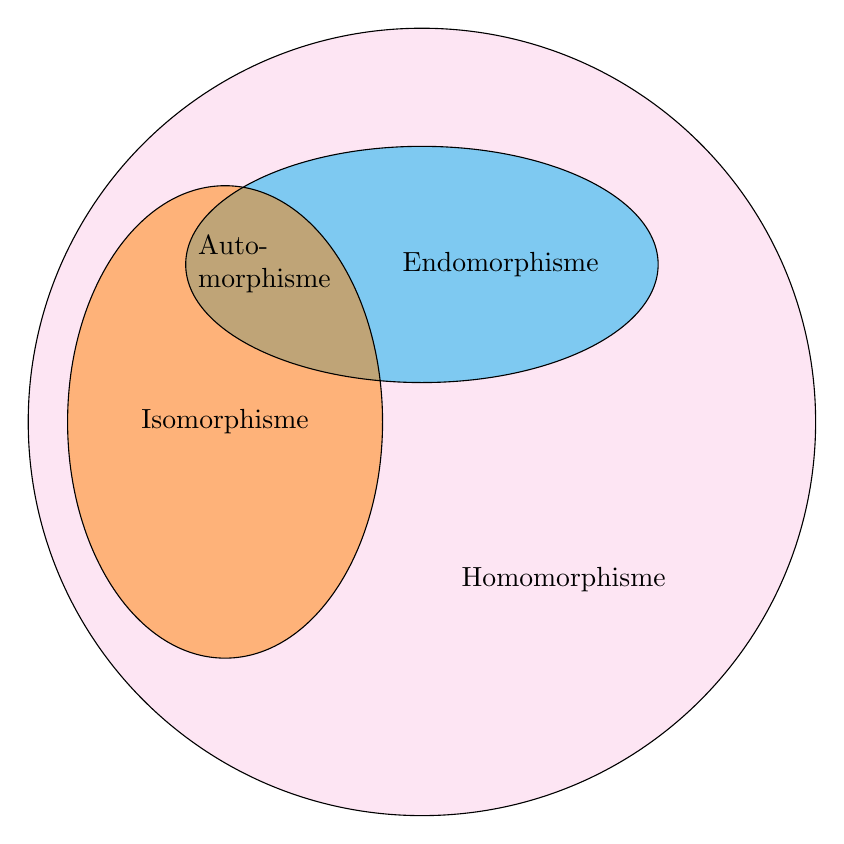
\begin{tikzpicture}
		\def\homomorphism{(0:0cm) circle (5.0cm)}
	  	\def\isomorphism{(180:2.5cm) ellipse (2.0cm and 3.0cm)}
	  	\def\endomorphism{(90:2.0cm) ellipse (3.0cm and 1.5cm)}
	      \begin{scope}[fill opacity=0.1]
	        \fill[magenta] \homomorphism;
	      \end{scope}
	
	      \begin{scope}[fill opacity=0.5]
	        \fill[cyan] \endomorphism;
	      \end{scope}
	
	      \begin{scope}[fill opacity=0.5]
	        \fill[orange] \isomorphism;
	      \end{scope}
	
	      \draw \homomorphism;
	      \draw \isomorphism;
	      \draw \endomorphism;
	
	      {
	        \scalefont{2.0}
	        \node[text=black] at ( 1.8,-2) {Homomorphisme};
	      }
	
	      {
	        \scalefont{1.6}
	        \node[text=black] at (-2.5, 0) {Isomorphisme};
	      }
	
	      {
	        \scalefont{1.4}
	        \node[text=black] at (   1, 2) {Endomorphisme};
	      }
	      \node[align=left] at (  -2, 2) {Auto-\\morphisme};
	    \end{tikzpicture}
		\caption[Diagramme de Venn de diff\'erents types d'homomorphismes]{Diagramme de Venn de diff\'erents types d'homomorphismes (source: Wikipédia, auteur: Martin Thoma}
	\end{figure}
	
	
	\subsubsection{Id\'eal}
	\textbf{D\'efinition (\#\mydef):}  Soit $A$ un anneau commutatif (comme $(\mathbb{R},+,\cdot)$ par exemple). Un sous-ensemble $S\subset A$ est un "\NewTerm{id\'eal}\index{id\'eal}" si:
	\begin{enumerate}
		\item[P1.] Pour tout $a,a'\in S$:
		
	
		\item[P2.] Pour tout $a\in S$ et tout $r\in A$:
		
	\end{enumerate}
	En d'autres termes, un id\'eal est un sous-ensemble ferm\'e pour l'addition et stable pour la multiplication par un \'el\'ement quelconque de $A$.
	\begin{tcolorbox}[colframe=black,colback=white,sharp corners]
	\textbf{{\Large \ding{45}}Exemple:}\\\\
	L'ensemble des nombres pairs $\mathbb{Z}_{2k}$ est par un exemple d'id\'eal de l'ensemble des nombres relatifs $\mathbb{Z}$.
	\end{tcolorbox}
	
	\begin{tcolorbox}[title=Remarque,colframe=black,arc=10pt]
	Les id\'eaux $S=\{0\}$ et $S=A$ sont appel\'es les  "\NewTerm{id\'eaux triviaux}".
	\end{tcolorbox}
	Pour savoir si un id\'eal est \'egal à tout l'anneau, il est utile d'utiliser la propri\'et\'e suivante qui sp\'ecifie que si $A$ est un anneau et $I$ un id\'eal de $A$, alors si $1\in A$ nous avons $I=A$.
	
	\begin{dem}
	Ceci r\'esulte de la propri\'et\'e P2 de la d\'efinition d'un id\'eal:
	
	Pour tout $r\in A$, nous avons $r=r\cdot 1\in 1$ car $1\in I$.
	\begin{flushright}
		$\blacksquare$  Q.E.D.
	\end{flushright}
	\end{dem}
	Un premier exemple d'id\'eal est donn\'e par le noyau d'un homomorphisme d'anneaux. Effectivement, d\'emontrons que le noyau d'un homomorphisme $F:R\mapsto S$ est un id\'eal de $R$.
	\begin{dem}
	$R$ $a,a'\in \ker (f)$. Alors:
	
	ce qui montre que $a+a'\in \ker(f)$. Soit $r\in R$, alors:
	
	ce qui montre que $r\cdot a\in \ker(f)$.
	\begin{flushright}
		$\blacksquare$  Q.E.D.
	\end{flushright}
	\end{dem}
	Proposition: Soit $A$ un anneau et soit $a\in A$. Le sous-ensemble:
	
	not\'e $(a)$ ou $aA$, est un id\'eal (nous allons voir un exemple concret après la prochaine d\'efinition).
	
	\textbf{D\'efinitions (\#\mydef):}
	\begin{enumerate}
		\item[D1.] Un id\'eal $I\neq A$ d'un anneau $A$ est dit "\NewTerm{"id\'eal principal}" s'il existe $a\in A$ tel que $I=(a)$.
	
		\item[D2.] Un anneau dont tous les id\'eaux sont principaux est dit "\NewTerm{anneau principal}".
	\end{enumerate}
	\begin{tcolorbox}[colframe=black,colback=white,sharp corners]
	\textbf{{\Large \ding{45}}Exemple:}\\\\
	Montrons maintenant que l’anneau $\mathbb{Z}$ est principal (car tous ses id\'eaux sont principaux).\\
	
	Soit $I$ un id\'eal de $\mathbb{Z}$  (il est facile d'en choisir un: par exemple, tous les multiples de $2$ ou $3$, etc.). Soit $r\in I$ le plus petit entier positif non nul de $I$. Nous montrerons que $I=r\mathbb{Z}=(r)$.\\
	
	Soit $a$, un \'el\'ement quelconque de $I$. La division euclidienne nous permet d'\'ecrire:
	
	avec $0\ge r' <r$ (comme nous l'avons d\'ejà prouv\'e).\\
	
	Mais comme $r'= a-qr$ et que $a, r \in I$, selon la d\'efinition d’un id\'eal, nous avons $ r' \in I$ (la somme ou la diff\'erence des \'el\'ements d'un id\'eal appartenant à l'id\'eal). Par le choix de $r$ ($r'$ \'etant inf\'erieur à $r$), cela signifie que $r' = 0$ et donc que $a = rq$.\\
	
	Ainsi, chaque \'el\'ement de $I$ est un multiple $r$ de $q$:
	
	Donc pour l'ensemble des nombres pairs (not\'es comme nous le savons par $2\mathbb{Z}$ ou $\mathbb{Z}_{2k}$) nous avons:
	
	\end{tcolorbox}
	L'exemple ci-dessus utilise uniquement la division euclidienne sur $\mathbb{Z}$. On peut alors g\'en\'eraliser ce r\'esultat aux anneaux qui possèdent une division euclidienne. Ainsi, par exemple, l'anneau $K[X]$ des polynômes (\SeeChapter{voir la section de Calcul Alg\'ebrique page \pageref{polynomial ring}}) avec des coefficients dans un corps $K$ est un anneau principal car il a une division euclidienne.

	\begin{theorem}
	L'anneau $K[X]$ des polynômes à coefficients dans un corps $K$ est un anneau principal (tous ses id\'eaux sont principaux).
	\end{theorem}
	\begin{dem}
	Soit $I$ un id\'eal de $K[X]$. Notons $d$ le plus petit degr\'e que puisse avoir un polynôme non nul de $I$. Si $d=0$ alors $1\in I$ et donc $I=1\cdot K[X]=K[X]$. Autrement, soit $a(X)$ un polynôme de degr\'e $d$. Si $u(X)\in I$ alors on peut diviser $u(X)$ par $a(X)$. Il existe $q(X),r(X)\in K[X]$ tels que $\deg(r)<\deg(a)=d$ et:
	
	Donc $r(X)\in I$ ce qui entraîne $r=0$ (autrement contradiction avec la minimalit\'e de $d$). Par suite:
	
	Nous venons de montrer que:
	
	\begin{flushright}
		$\blacksquare$  Q.E.D.
	\end{flushright}
	\end{dem}
	Pour en revenir à $\mathbb{Z}$... nous venons alors de prouver que les seuls id\'eaux sont ceux de la forme $r\mathbb{Z}$. De plus si nous avons $d$ et  $r$ qui sont des entiers $>1$. Alors $r\mathbb{Z}\subset d\mathbb{Z}$ si et seulement si $d | r$.
	\begin{dem}
	Si $d | r$ alors il existe $n$ avec $r=d\cdot n$. Soit $m\cdot a$ un \'el\'ement de $r\mathbb{Z}$. Alors:
	
	ce qui montre que $r\mathbb{Z}\subset d\mathbb{Z}$.

	R\'eciproquement, si $r\in d\mathbb{Z}$ ceci implique que $r$ est de la forme $d\cdot n$ et ceci prouve que $d$ divise $r$.
	\begin{flushright}
		$\blacksquare$  Q.E.D.
	\end{flushright}
	\end{dem}
	\begin{theorem}
	D\'emontrons aussi qu'un anneau $R$ est un corps si et seulement s'il ne possède que les id\'eaux triviaux:
	
	\end{theorem}
	\begin{dem}
	Montrons que la condition est n\'ecessaire: Soit $I$ un id\'eal non nul de $R$ (c'est-à-dire diff\'erent de $\{0\}$) et $r\in I$ un \'el\'ement non nul. Par hypothèse (qu'il s'agit d'un corps), il est inversible, c'est-à-dire qu'il existe $t\in R$ tel que:
	
	Ceci implique que $1\in I$ et donc, par un r\'esultat obtenu plus haut $I=R$.
	
	R\'eciproquement, supposons que tout id\'eal $I\neq R$ soit l'id\'eal nul (c'est-à-dire $\{0\}$). Alors si $r\in R$ est un \'el\'ement non nul de $R$, l'id\'eal principal $(r)$ doit être \'egal à $R$. Mais ceci implique que $1\in (r)$ et donc qu'il existe $x\in R$ avec $r\cdot x=1$ ce qui montre que $r$ est inversible. L'anneau $R$ est donc un corps.
	\begin{flushright}
		$\blacksquare$  Q.E.D.
	\end{flushright}
	\end{dem}
	Cette caract\'erisation va nous permettre de d\'emontrer relativement facilement que:
	\begin{theorem}
	Tout homomorphisme partant d'un corps est injectif. Soit que si $f:R\mapsto S$ est un homomorphisme où $R$ est un corps, alors $f$ est injectif.
	\end{theorem}
	\begin{dem}
	Nous mettons ensemble ce qui a \'et\'e vu jusque-là:
	\begin{itemize}
		\item Nous avons d\'emontr\'e plus haut que le noyau $\ker(f)$ d'un homomorphisme d'anneau est un id\'eal.
	
		\item Mais nous avons \'egalement d\'emontr\'e plus haut qu'un ensemble \'etait un corps si $\{0\}$ et $R$ sont les seuls triviaux id\'eaux.
	\end{itemize}
	Dès lors pour les deux points, nous avons soit $\ker(f)=0$ ou $\ker(f)=R$ pour le corps (\'etant donn\'e qu'il inclut le concept d'anneau!).
	
	Mais vu que $f(1)=1\neq 0$ (de par la d\'efinition d'un homomorphisme) il s'ensuit qu'il reste $\ker(f)=\{0\}$ (puisque nous avons d\'emontr\'e que si $A$ est un anneau et $I$ un id\'eal de $A$ alors si $1\in I$ alors $I=R$). Ceci implique par un th\'eorème pr\'ec\'edent (où nous avons d\'emontr\'e que si $\ker(f)=\{0\}$ l'homomorphisme est injectif) que... $f$ est injective.
	\begin{flushright}
		$\blacksquare$  Q.E.D.
	\end{flushright}
	\end{dem}
	\'etudions maintenant les homomorphismes dont l'anneau de d\'epart est $\mathbb{Z}$. Soit $A$ un anneau et $f:\mathbb{Z}\mapsto A$  un homomorphisme. Par d\'efinition d'un homomorphisme et par ses propri\'et\'es, il faut que $f(0)=0$ et $f(1)=1$ (parmi d'autres). Mais il faut encore que:
	
	pour tout $k\in\mathbb{Z}$. Ainsi $f$ est complètement d\'etermin\'e par la donn\'ee de $f(1)$ et est donc unique. R\'eciproquement, nous montrons que l'application $f:\mathbb{Z}\mapsto A$ d\'efinie par:
	
	est un homomorphisme d'anneaux. En r\'esum\'e, il existe un et un seul homomorphisme de $\mathbb{Z}$ dans un anneau quelconque $A$.
	
	\textbf{D\'efinition (\#\mydef):} Soient $A$ un anneau et $f:\mathbb{Z}\mapsto A$ l'unique homomorphisme d\'efini pr\'ec\'edemment. Si $f$ est injectif, nous dirons que $A$ est de "\NewTerm{caract\'eristique nulle}\index{caract\'eristique nulle}" et nous notons cela:
	
	Sinon, $\ker(f)$ est un id\'eal non trivial de $\mathbb{Z}$ et comme $\mathbb{Z}$ est dès lors principal (comme nous l'avons d\'emontr\'e plus haut) il est de la forme $k\mathbb{Z}$ avec $k>0$. L'entier $k$ est appel\'e la "\NewTerm{caract\'eristique de $A$}\index{caract\'eristique}" et nous avons alors:
	
	\begin{tcolorbox}[title=Remarque,colframe=black,arc=10pt]
	Moins formellement, la caract\'eristique d'un anneau $A$ est le plus petit entier positif $k$ tel que $k\cdot 1_A=0$. S'il n'y en a pas, alors la caract\'eristique est nulle.
	\end{tcolorbox}	
	La d\'efinition ci-dessus n'est peut-être pas très claire (du moins pour moi cela ne l'est pas!). Voyons donc une autre approche pour introduire la caract\'eristique beaucoup plus d\'etaill\'ee ...:
	
	Soit $A$ un anneau et n'importe lequel de ses \'el\'ements $a$, d\'esignons les entiers dans ce qui va suivre en gras. Ainsi, $\pmb{1}$ est le nombre entier un, par exemple, $\pmb{0}$ est le nombre entier z\'ero, alors que $0_A$ et $1_A$ sont les \'el\'ements neutres de $A$.

	Comme $A$ sous l'addition est un groupe ab\'elien, on peut d\'efinir comme d'habitude:
	
	Par d\'efinition d’un homomorphisme, nous avons si $ f:\mathbb{Z}\mapsto A$ que:
	
	alors pour rappel:
	\begin{itemize}
		\item $f(\pmb{m}+\pmb{n})=f(\pmb{m})+f(\pmb{n})$
		\item $f(\pmb{mn})=f(\pmb{m})f(\pmb{n})$
		\item $f(\pmb{1})=1_A$
	\end{itemize}
	donc si $f$ est un homomorphisme d'anneaux. Comme tous les homomorphismes d'anneau, $f:\mathbb{Z}\mapsto A$ a un noyau qui est un id\'eal, comme nous venons de le prouver, donc nous avons $\ker(f)=\pmb{k}\mathbb{Z}$ pour un unique $\pmb{k}\ge\pmb{0}$.
	
	Si $k=0$ alors, comme nous l'avons prouv\'e beaucoup plus haut, $f$ est injectif. Sinon, nous avons:
	
	par d\'efinition du noyau, ce qui signifie que:
	
	pour chaque $a\in A$. Cet entier $\pmb{k}$ est la "caract\'eristique" de $S$.
	
	C'est-à-dire que $\text{char}(A)$ est le plus petit nombre positif $\pmb{k}$ tel que:
	
	si un tel nombre $\pmb{k} \in \mathbb{N}$ existe, et $0$ sinon.
	
	\begin{tcolorbox}[colframe=black,colback=white,sharp corners]
	\textbf{{\Large \ding{45}}Exemples:}\\\\
	E1. Le seul anneau qui a $\text{char}(A)=1$ tel que:
	
	est l'anneau trivial $A=\{0_A\}$.\\
	
	E2. L'anneau $\mathbb{Z}$ a la caract\'eristique z\'ero car l'homomorphisme unique $f:\mathbb{Z} \mapsto\mathbb{Z}$ est l'identit\'e. C'est donc injectif.\\
	
	E3. Les injections $\mathbb{Z}\mapsto \mathbb{Q}$ et $\mathbb{Z}\mapsto \mathbb{R}$ montrent que $\mathbb{Q}$ et $\mathbb{R}$ (et $\mathbb{C}$ \'egalement) sont des corps de caract\'eristique nulle.
	\end{tcolorbox}
	\begin{theorem}
	Nous nous proposons maintenant de d\'emontrer que la caract\'eristique d'un anneau intègre (et en particulier d'un corps) est \'egale $0$ ou à un premier $p$.
	\end{theorem}
	\begin{dem}
	Nous montrons la contrapos\'ee. Soit $A$ un anneau de caract\'eristique $m\neq 0$ avec $m$ non premier.
	
	Il existe alors des entiers naturels $n,r\in\mathbb{N}$ contraints par $n,r<m$ tels que $m=n\cdot r$.

	Soit $f:\mathbb{Z}\mapsto A$ l'unique homomorphisme (d\'efini pr\'ec\'edemment). Par d\'efinition (de l'id\'eal) de $m$, nous avons $f(m)=0_A$ mais (!) $f(r)\neq 0 \neq f(n)$. Mais alors (et c'est là le truc de la preuve!):
	
	ce qui montre que $A$ n'est pas intègre.
	\begin{flushright}
		$\blacksquare$  Q.E.D.
	\end{flushright}
	\end{dem}
	\begin{tcolorbox}[title=Remarque,colframe=black,arc=10pt]
	La r\'eciproque du th\'eorème n'est pas vraie comme le montre l'exemple de l'anneau $\mathbb{R}\times\mathbb{R}$ où l'addition et la multiplication se font composante par composante. C'est un anneau de caract\'eristique nulle mais avec des diviseurs de z\'ero:
	
	\end{tcolorbox}	
	
	
	\begin{flushright}
	\begin{tabular}{l c}
	\circled{95} & \pbox{20cm}{\score{4}{5} \\ {\tiny 16 votes, 62.5\%}} 
	\end{tabular} 
	\end{flushright}

	%to make section start on odd page
	\newpage
	\thispagestyle{empty}
	\mbox{}
	\section{Probabilit\'es}\label{probabilities}
	\lettrine[lines=4]{\color{BrickRed}L}e calcul des probabilit\'es s'occupe des ph\'enomènes al\'eatoires (dits plus esth\'etiquement: "\NewTerm{processus stochastiques}\index{processus stochastiques}" lorsqu'ils sont d\'ependants du temps), c'est-à-dire de ph\'enomènes qui ne mènent pas toujours à la même issue et qui peuvent être \'etudi\'es grâce aux nombres et à leurs cons\'equences et apparitions. N\'eanmoins, même si ces ph\'enomènes ont des issues vari\'ees, d\'ependant du hasard, nous observons cependant une certaine r\'egularit\'e statistique.

	La probabilit\'e est quantifi\'ee comme un nombre compris entre $0$ et $1$ (où $0$ indique l'impossibilit\'e et $1$ indique la certitude). Plus la probabilit\'e d'un \'ev\'enement est \'elev\'ee, plus nous sommes certains que l'\'ev\'enement se produira.
	
	Les probabilités sont très importantes dans la pratique, en particulier à un niveau très élevé de gestion d'entreprise ou politique. En effet, dans de nombreux cas, il est plus pratique d'utiliser une règle simple mais incertaine plutôt qu'une règle complexe mais certaine, même si la vraie règle est déterministe et notre système de modélisation a la fidélité de s'adapter à une règle complexe. Par exemple, la règle simple "les ventes augmenteront" est peu coûteuse à développer et est largement utile, tandis qu'une règle de la forme ", les ventes augmenteront si l'indice d'inflation augmente également, et qu'il n'y a pas d'épidémie, pas de tremblements de terre, pas de conflits, pas d'astéroïdes, pas d'inondations majeures, pas de changements politiques, pas de grèves ..." coûte cher à développer, à entretenir et à communiquer, et après tout cet effort le modèle sera encore très fragile et sujet à l'échec.
	
	Les concepts li\'es aux probabilit\'es ont reçu une formalisation math\'ematique axiomatique en th\'eorie des probabilit\'es (voir plus bas), largement utilis\'ee dans des domaines d’\'etudes tels que les math\'ematiques, la statistique, la finance, les jeux de hasard, les sciences (en particulier la physique), l’intelligence artificielle / l'apprentissage machine, l'informatique, la th\'eorie des jeux et la philosophie pour, par exemple, tirer des conclusions sur la fr\'equence attendue des \'ev\'enements. La th\'eorie des probabilit\'es est \'egalement utilis\'ee pour d\'ecrire les m\'ecanismes sous-jacents et les r\'egularit\'es de systèmes complexes.

	\textbf{D\'efinitions (\#\mydef):} Il existe plusieurs manières de d\'efinir une probabilit\'e. Principalement, nous parlons de:
	\begin{itemize}
		\item[D1.] "\NewTerm{Probabilit\'e exp\'erimentale ou inductive}\index{probabilit\'e inductive}" qui est la probabilit\'e d\'eduite de toute la population concern\'ee.
	
		\item[D2.] "\NewTerm{Probabilit\'e th\'eorique ou d\'eductive}\index{probabilit\'e d\'eductive}" qui est la probabilit\'e connue grâce à l'\'etude du ph\'enomène sous-jacent sans exp\'erimentation. Il s'agit donc d'une connaissance "a priori" par opposition à la d\'efinition pr\'ec\'edente qui faisait plutôt r\'ef\'erence à une notion de probabilit\'e "à posteriori".
	\end{itemize}
	Comme il n'est pas toujours possible de d\'eterminer des probabilit\'es a priori, nous sommes souvent amen\'es à r\'ealiser des exp\'eriences. Il faut donc pouvoir passer de la première à la deuxième solution. Ce passage est suppos\'e possible en termes de limite (avec une population dont la taille tend vers la taille de la population r\'eelle).
	
	La mod\'elisation formelle par le calcul des probabilit\'es a \'et\'e invent\'ee par A.N. Kolmogorov dans un livre paru en 1933. Cette mod\'elisation est faite à partir de l'espace de probabilit\'es ($U$, $A$, $P$) que nous d\'efinirons plus loin et que nous pouvons relier à la th\'eorie de la Mesure (voir section du même nom page \pageref{measure theory}). Cependant, les probabilit\'es ont \'et\'e \'etudi\'ees sur le point de vue scientifique par Pierre deFermat et Blaise Pascal au milieu du 17ème siècle.

	\begin{tcolorbox}[title=Remarque,colframe=black,arc=10pt]
	Si vous avez un professeur ou un formateur qui ose vous enseigner les statistiques et probabilit\'es avec des exemples bas\'es sur des jeux de hasard (cartes, d\'es, allumettes, pile ou face, etc.) d\'ebarrassez-vous en ou d\'enoncez-le à qui de droit car cela signifierait qu'il n'a aucune exp\'erience pratique du domaine et qu'il va vous enseigner n'importe quoi et n'importe comment (normalement les exemples devraient être bas\'es sur l'industrie, l'\'economie ou la R\&D, bref dans des domaines utilis\'es tous les jours par les entreprises mais surtout pas sur des jeux de hasard...!).
	\end{tcolorbox}	
	
	\subsection{Univers des \'ev\'enements}

	\textbf{D\'efinitions (\#\mydef):}

	\begin{itemize}
		\item[D1.]  "\NewTerm{L'univers des \'ev\'enements}\index{univers des \'ev\'enements}", ou "\NewTerm{univers des observables}\index{univers des observables}", $U$ est l'ensemble de toutes les issues (r\'esultats) possibles, appel\'ees "\'ev\'enements \'el\'ementaires", qui se pr\'esentent au cours d'une \'epreuve al\'eatoire d\'etermin\'ee. L'univers peut être fini (d\'enombrable) si les \'ev\'enements \'el\'ementaires sont en nombre fini ou continu (non d\'enombrable) s'ils sont infinis.
	
		\item[D2.] Un "\NewTerm{\'ev\'enement}\index{\'ev\'enement}" quelconque $A$ est un ensemble d'\'ev\'enements \'el\'ementaires et constitue une partie de l'univers des possibles $U$. Il est possible qu'un \'ev\'enement ne soit constitu\'e que d'un seul \'ev\'enement \'el\'ementaire.
	\end{itemize}

	\begin{tcolorbox}[colframe=black,colback=white,sharp corners]
	\textbf{{\Large \ding{45}}Exemples:}\\\\
	E1. Consid\'erons l'univers de tous les groupes sanguins possible, alors l'\'ev\'enement $A$ "l'individu est de rh\'esus positif" est repr\'esent\'e par:
	
	alors que l'\'ev\'enement $B$ "l'individu est donneur universel" est repr\'esent\'e par:
	
	qui constitue donc un \'ev\'enement \'el\'ementaire.\\
	
	E2. Dans $(\mathbb{N},+)$ chaque \'ev\'enement est r\'egulier et dans $(\mathbb{N},\times)$ tout \'ev\'enement non-nul est r\'egulier.
	\end{tcolorbox}
	
\begin{itemize}
	\item[D3.] Soit $U$ un univers et $A$ un \'ev\'enement, nous disons que l'\'ev\'enement $A$ "à lieu" (ou "se r\'ealise") si lors du d\'eroulement de l'\'epreuve se pr\'esente l'issue $i\:\left( i \in U \right)$ et que $i \in A$. Dans le cas contraire, nous disons que $A$ "n'a pas lieu" (ou "ne s'est pas r\'ealis\'e").

	\item[D4.] Le sous-ensemble vide $\varnothing$ de $U$ s'appelle "\NewTerm{\'ev\'enement impossible}\index{\'ev\'enement impossible}". En effet, si lors de l'\'epreuve l'issue $i$ se pr\'esente, nous avons toujours $i \in \varnothing$ et l'\'ev\'enement $\varnothing$ n'a donc jamais lieu.\\
	
	Si $U$ est fini, ou infini d\'enombrable, tout sous-ensemble de $U$ est un \'ev\'enement, ce n'est plus vrai si $U$ est non d\'enombrable (nous verrons dans le chapitre de Statistiques pourquoi).

	\item[D5.] L'ensemble $U$ s'appelle aussi  "\NewTerm{\'ev\'enement certain}\index{\'ev\'enement certain}". En effet, si lors de l'\'epreuve l'issue $i$ se pr\'esente, nous avons toujours $i\in U$ (car $U$ est l'univers des \'ev\'enements). L'\'ev\'enement $U$ a donc toujours lieu!

	\item[D6.] Soit $A$ et $B$ deux sous-ensembles de $U$. Nous savons que les \'ev\'enements   $A \cup B$ et $A \cap B$ sont tous deux des sous-ensembles de $U$ donc des \'ev\'enements qui sont respectivement des "\NewTerm{\'ev\'enements conjoints}\index{\'ev\'enements conjoints}" et des "\NewTerm{\'ev\'enements disjoints}\index{\'ev\'enements disjoints}\label{disjoint events}".
	
	\item[D7.] Si deux \'ev\'enements $A$ et $B$ sont tels que:
	
	les deux \'ev\'enements ne peuvent pas être r\'ealisables pendant la même \'epreuve, nous disons alors qu'ils sont des "\NewTerm{\'ev\'enements incompatibles}\index{\'ev\'enements incompatibles}".

	\item[D8.] Si deux \'ev\'enements $A$ et $B$ sont tels que:
	
	les deux \'ev\'enements peuvent être r\'ealisables dans la même \'epreuve (possibilit\'e de voir un chat noir au moment où on passe sous une \'echelle par exemple...), nous disons inversement qu'ils sont des "\NewTerm{\'ev\'enements ind\'ependants}\index{\'ev\'enements ind\'ependants}".
	
	\item[D9.] Le "\NewTerm{hasard}\index{hasard}" est le manque de structure ou de pr\'evisibilit\'e dans les \'ev\'enements. Une s\'equence al\'eatoire d'\'ev\'enements, de symboles ou d'\'etapes n'a pas d'ordre et ne suit pas un modèle ou une combinaison intelligible. Les \'ev\'enements individuels al\'eatoires sont par d\'efinition impr\'evisibles, mais dans de nombreux cas, la fr\'equence de r\'esultats diff\'erents sur un grand nombre d'\'ev\'enements (ou "essais") est pr\'evisible.
	
	\begin{tcolorbox}[title=Remarque,colframe=black,arc=10pt]
	Si nous choisissons al\'eatoirement (uniform\'ement) un nombre r\'eel dans l’intervalle $[0,1]$, il existe une probabilit\'e nulle que nous choisissions ce nombre. Cela ne signifie pas que nous n'avons pas choisi de num\'ero du tout!\\

	De même avec les rationnels, bien qu'infinis, et denses et tout cela, ils sont très très rares en termes de mesure et de probabilit\'e. Il est parfaitement possible que si nous lançons d'innombrables fl\'echettes sur la ligne r\'eelle, nous atteindrons exactement tous les rationnels et chaque rationnel exactement une fois. Ce sc\'enario est hautement improbable, car les nombres rationnels correspondent à une mesure nulle.\\

	Le domaines des probabilit\'es standard traite avec \textit{quelles sont les chances que cela se produise}? \underline{a priori}, pas a posteriori (cela est le rôle des probabilit\'es bay\'esiennes)!! Nous sommes donc int\'eress\'es par la mesure d’une certaine structure d'un ensemble, dans les aspects modernes de probabilit\'e et de mesure, les nombres rationnels ont une taille \'egale à z\'ero, ce qui signifie une probabilit\'e nulle. De manière plus formelle, comme nous le verrons dans la section de Statistiques à la page \pageref{probability density function}, les probabilit\'es sont obtenues en int\'egrant une fonction de densit\'e de probabilit\'e $f(x)$ sur un intervalle. La fonction est non n\'egative et a la propri\'et\'e:
	
	La probabilit\'e de s\'electionner un r\'eel dans un intervalle $[a,b]\subset \mathbb{R}$ est alors donn\'ee par:
	
	Le lecteur peut voir maintenant que, \'etant donn\'e un nombre r\'eel $x_0\in\mathbb{R}$, nous avons:
		
	\end{tcolorbox}	
\end{itemize}

	\pagebreak
	\subsubsection{Paradoxe du singe savant (loi de Borel)}
	Le "pradoxe du singe savant" stipule qu'un singe frappant des touches de manière al\'eatoire sur un clavier de machine à \'ecrire pendant une dur\'ee infinie tapera presque sûrement un texte donn\'e, tel que l'oeuvre complète de William Shakespeare. En fait, le singe taperait sûrement tous les textes finis possibles un nombre infini de fois. Cependant, la probabilit\'e qu'un Univers rempli de singes dactylographiant une oeuvre complète telle que le \textit{Hamlet} de Shakespeare est si infime que la chance qu'elle se produire au cours d'une p\'eriode de plusieurs centaines de milliers d'ordres de plus que l’âge de l'Univers est extrêmement faible ( mais techniquement pas z\'ero!).
	
	Dans ce contexte, "presque sûrement" est un terme math\'ematique avec une signification pr\'ecise, et le "singe" n'est pas un singe r\'eel, mais une m\'etaphore d'un dispositif abstrait produisant une s\'equence al\'eatoire infinie de lettres et de symboles.
	
	\begin{theorem}
	Si nous avons un nombre infini de singes frappant des touches au hasard sur des claviers de machine à \'ecrire, alors, avec une probabilit\'e de $1$, l'un d'entre eux dactylographiera les oeuvres complètes de William Shakespeare (finirait par \'ecrire tout livre qui ait jamais exist\'e, avec suffisamment de temps).
	\end{theorem}

	\begin{dem}
	Soit $A_n$ l'\'ev\'enement où $n$-ème singe tape l'oeuvre complète de Shakespeare. Ensuite, s'il y a $m$ caractères sur le clavier et $N$ caractères dans les oeuvres complètes de Shakespeare, la probabilit\'e d'obtenir les oeuvres complètes de Shakespeare devrait être de:
	
	pour chaque $n$. De plus, les $A_n$ sont mutuellement ind\'ependants (\'ev\'enements disjoints). Par cons\'equent:
	
	Un nombre infini d'\'ev\'enements $A_n$ se produisent, c'est-à-dire qu'un nombre infini de singes dactylographient les oeuvres complètes de Shakespeare.
	\begin{flushright}
		$\blacksquare$  Q.E.D.
	\end{flushright}
	\end{dem}
	Par cons\'equent, si nous acceptons l'infini dans un argument, nous pouvons alors accepter \'egalement que "l'infini \'etant donn\'e, tout peut arriver".
	
	\begin{tcolorbox}[title=Remarque,colframe=black,arc=10pt]
	Ce résultat est un cas particulier d'un résultat plus général nommé "\NewTerm{second lemme de Borel–Cantelli}\index{second de lemme Borel–Cantelli}". Ce lemme énonce que si les événements $E_n$ sont indépendants et que la somme des probabilités des $E_n$ diverge à l'infini, alors la probabilité qu'une infinité d'entre eux se produisent est de $1$. C'est-à-dire si $\sum_{n=1}^{+\infty} P\left(E_{n}\right)=+\infty$ et les événements $\left(E_{n}\right)_{n =1}^{+\infty}$ sont indépendants, alors $P\left(\limsup _{n \rightarrow +\infty} E_{n}\right)=1$. Formellement:
	
	\end{tcolorbox}
	
	\pagebreak
	 \subsubsection{Est-ce que les probabilit\'es r\'efutent les structures complexes?}
	 \begin{fquote} [P. S. de Laplace] Les questions les plus importantes de la vie ne sont en effet, pour la plupart, en réalité que des problèmes de probabilité.\end{fquote}
	 Les créationnistes traditionnels et les auteurs de livres sur Design Intelligent invoquent régulièrement des arguments de probabilité dans les critiques de l'évolution biologique. Ils soutiennent que certaines caractéristiques de la biologie sont si incroyablement improbables qu'elles n'auraient jamais pu être produites par un processus "naturel" purement aléatoire, même en supposant les milliards d'années d'histoire confirmées par les géologues et les astronomes. Ils assimilent souvent l'hypothèse d'évolution à la suggestion absurde que des singes tapant au hasard sur une machine à écrire pourraient composer une sélection des travaux de Shakespeare, ou qu'une explosion dans un parc d'équipements aérospatiaux pourrait produire un avion de ligne 747 fonctionnel (nous ne citerons pas les gens qui ont écrit cela parce que la qualité de leur contenu ne mérite pas d'être cité ici et cela pourrait leur faire de la publicité!). Des écrits plus récents de ce genre, dans le but de promouvoir une vision du monde de la "conception intelligente", soutient que la biologie fonctionnelle fonctionne sur un sous-ensemble extrêmement petit de l'espace de toutes les séquences d'ADN possibles, et que toute modification du "programme informatique" de la biologie sont, comme les changements apportés aux programmes informatiques humains, presque certains de rendre l'organisme non fonctionnel (encore une fois, nous ne citerons pas les écrits des personnes qui ont écrit cela pour les mêmes raisons qu'auparavant!).
	
	Bien que le public en général ne l'apprécie généralement pas, il est bien connu dans le monde de la recherche scientifique que les arguments fondés sur les probabilités et les statistiques sont chargés de biais et d'erreurs potentielles, et même les chercheurs "experts" peuvent se tromper avec un raisonnement invalide. Pour ces raisons, des cours rigoureux de probabilités et de statistiques sont désormais exigés des étudiants dans pratiquement tous les domaines scientifiques (gardez à l'esprit que l'ingénierie n'est pas une science, c'est pourquoi en fait la grande majorité des ingénieurs ont une très faible compréhension des probabilités et des statistiques) , ainsi que dans de nombreuses autres disciplines. Les avocats doivent être au moins modérément familiarisés avec les arguments de probabilité et de statistiques étant donné que ces derniers peuvent mal compris dans les arguments rhétoriques. Dans le monde de la finance, le surajustement statistique et d'autres erreurs de probabilité et statistiques sont désormais considérés comme l'une des principales raisons du fait que de nombreuses stratégies et fonds d'investissement qui ont fière allure sur papier échouent souvent lamentablement dans l'utilisation dans le monde réel.
	
	Pour illustrer les difficultés avec les arguments de probabilité, les professeurs de mathématiques demandent souvent à leur classe (disons qu'elle compte $23$ élèves) s'ils pensent qu'il est probable que deux personnes ou plus dans la classe aient exactement la même date d'anniversaire. La plupart des étudiants disent que c'est très peu probable, pensant que les chances que deux personnes aient le même anniversaire particulier sont de $1 /365 $, et donc $23$ fois cette quantité n'est que de $23/365 $. Mais cet argument est fallacieux, en effet, si l'on numérote les $23$ personnes de $1$ à $23$, l'événement selon lequel toutes $23$ personnes ont des anniversaires différents est le même que l'événement où la personne $2$ n'a pas la même date d'anniversaire que la personne $ 1 $, et que personne $ 3 $ n'a pas la même date d'anniversaire que la personne $ 1 $ ou la personne $ 2 $, et ainsi de suite, et finalement que le personne $ 23 $ n'a pas le même anniversaire que les personnes de $ 1 $ à $ 22 $.
	
	Appelons ces événements respectivement "Événement $ 2 $", "Événement $ 3 $", etc. On peut également ajouter un "Événement 1", correspondant à l'événement de la personne $ 1 $ ayant une date d'anniversaire, qui se produit avec la probabilité $ 1 $. Cette conjonction d'événements peut être calculée en utilisant une probabilité conditionnelle: la probabilité de l'Événement $2$ est de $364/365$, car la personne $2$ peut avoir une date d'anniversaire autre que la date d'anniversaire de la personne $1$. De même, la probabilité de l'Événement $ 3 $ étant donné que l'Événement $ 2 $ survenu est de $  363 / 365 $, car la personne $ 3 $ peut avoir l'une des dates d'anniversaires non déjà prises par les personnes $ 1 $ et $ 2 $. Cela continue jusqu'à ce que finalement la probabilité de l'Événement $ 23 $ étant donné que tous les événements précédents se soient produits est $ 343/365 $. Enfin, le principe de probabilité conditionnelle implique que la probabilité $ P (A ') $ que deux personnes dans la pièce n'aient pas le même anniversaire est égale au produit de ces probabilités individuelles:
	
	Par conséquent, la probabilité qu'au moins deux personnes de la classe aient la même date d'anniversaire est donnée par (car les deux événements s'excluent mutuellement):
	
	Un argument typique de conception intelligence des créationnistes (argument de niveau école secondaire ...) se présente ainsi: la molécule d'alpha-globine humaine (abrégé HBA1), un composant de l'hémoglobine qui remplit une fonction clé de transfert d'oxygène, est une chaîne protéique basée sur une séquence de $ 141 $ acides aminés \footnote{La molécule d'hémoglobine est composée de quatre chaînes polypeptidiques: deux chaînes alpha de 141 résidus d'acides aminés chacune et deux chaînes bêta de 146 résidus d'acides aminés chacune}. Il existe $20$ différents acides aminés communs dans les systèmes vivants:
	\begin{figure}[H]
		\centering
		\includegraphics[width=0.70\textwidth]{img/arithmetics/amino_acids.jpg}
		\caption[Acides aminés courants]{Acides aminés courants (auteur: ?)}
	\end{figure} 
	Avec le séquençage de l'alpha-globine qui est:
	
	\texttt{Val-Leu-Ser-Pro-Ala-Asp-Lys-Thr-Asn-Val-Lys-Ala-Ala-Trp-Gly-Lys-Val-Gly\\
	-Ala-His-Ala-Gly-Glu-Tyr-Gly-Ala-Glu-Ala-Leu-Glu-Arg-Met-Phe-Ser-Phe-Pro\\
	-Thr-Thr-Lys-Thr-Tyr-Phe-Pro-His-Phe-Leu-Ser-His-Gly-Ser-Ala-GIn-Val-Lys\\
	-Gly-His-Gly-Lys-Lys-Lys-Val-Ala-Asp-Ala-Leu-Thr-Ala-Val-His-Val-Hal-Hal\\
	-Hsp-Met-Pro-Asn-Ala-Leu-Ser-Ala-Leu-Ser-Asp-Leu-His-Ala-Heu-Arg-Val-Asp\\
	-Pro-Val-Asn-Phe-Lys-Leu-Leu-Ser-His-Cys-Leu-Leu-Leu-Ala-His-Leu-Pro-Ala\\
	-Glu-Phe-Thr-Pro-Ala-Val-His-Ala-Ser-Leu-Asp-Lys-Phe-Leu-Ala-Ser-Val-Ser\\
	-Thr-Val-Leu-Thr-Ser-Lys-Tyr-Arg}
	
	Ou pour une version abrégée des quatre chaînes polypeptidiques:
	\begin{itemize}
		\item Chaîne A:\\
		\texttt{VLSPADKTNV KAAUGKVGAH AGEYGAEALE RMFLSFPTTK TYFPHFDLSH GSAOVKGHGK KVADALTHAV AHVDDMPMAL SALSDLHAHK LRVDPVNFKL. LSHCLLVTLA AHLPAEFTPA VHASLDKFLA SVSTVLTSKY R}
		
		\item Chaîne B:\\
		\texttt{VHLTPEEKSA VTALUGKVNV DEVGGEALGR LLVVYPUTOR FFESFGDLST pDAVHGWRV KAHGKKWLGA FSDGLAHLDN LKGTFATLSE LHCDKLHWDP ENFRLLGNVL VCVLAHHFGK EFTPPVOAAY OKVVAGVANA LAHKYH}
		
		\item Chaîne C:\\
		\texttt{WLSPADKTNV KAAUGKVGAH AGEYGAEALE RMFLSFPTTK TYFPHFDLSH GSAOVKGHGK KVADALTNAV AHVDDHPNAL SALSDLHAHK LRVDPVNFKL LSHCLLVTLA AHLPAEFTPA VHASLDKFLA SVSTVLTSKY R}
		
		\item Chaîne D:\\
		\texttt{WHLTPEEKSA VTALUGKVNV DEVGEEALGR LLWYPUTOR FFESFGDLST PDAVMGNPKV KAHGKKVLGA FSDGLAHLDN LKGTFATLSE LHCDKLHVDP ENFRLLGNVL VCVLAHHFGK EFTPPVQ}
	\end{itemize}
	
	Donc, le nombre de chaînes potentielles de longueur $ 141 $ est\footnote{Ce calcul est de toute façon relataviment faux car les permutations symétriques (résultats miroir) sont comptés - mais cela ne changera cependant pas l'ordre de grandeur du résultat - et des preuves expérimentales ont montré qu'il existe des séquences d'acides aminés interdites et/ou instables!} (voir plus bas page \pageref{simple arrangements with repetitions} pour la preuve):
	
	Les créationnistes et aussi de nombreux autres théistes soutiennent alors que ce chiffre est si énorme que même après des milliards d'années d'essais moléculaires aléatoires, aucune molécule de protéine alpha-globine humaine n'apparaîtrait jamais "au hasard", et donc l'hypothèse que l'alpha-globine humaine est née par un processus évolutif est réfuté de manière décisive.
	
	Une erreur majeure dans l'argument alpha-globine mentionné ci-dessus, commun à beaucoup d'autres de ce genre, est qu'il ignore le fait qu'une grande classe de molécules d'alpha-globine peut remplir la fonction essentielle de transfert d'oxygène, de sorte que le calcul de la probabilité d'une seule instance est trompeuse a priori. En effet, la plupart des $141$ acides aminés dans l'alpha-globine peuvent être modifiés sans altérer la fonction clé de transfert d'oxygène, comme on peut le constater en notant la grande variété de molécules d'alpha-globine à travers le règne animal. Quand on révise le calcul ci-dessus, sur la base de seulement $25$ emplacements essentiels à la fonction de transport d'oxygène (ce qui est une surestimation généreuse), on obtient $10^{33}$ chaînes fondamentalement différentes, un chiffre énorme mais incomparablement plus petit que $10^{183}$.
	
	Un calcul comme celui-ci peut être affiné davantage, en tenant compte d'autres caractéristiques de l'alpha-globine et de sa biochimie associée. Certains de ces calculs produisent des valeurs de probabilité encore plus extrêmes que les précédentes. Mais un de ces calculs est-il vraiment important? Le problème principal est que tous ces calculs, qu'ils soient effectués avec précision ou non, souffrent de l'erreur fatale de présumer qu'une structure telle que l'alpha-globine humaine est née d'un seul événement d'essai aléatoire tout-en-un. Mais générer une molécule "au hasard" en un seul coup n'est décidément pas l'hypothèse scientifique en question - c'est une théorie créationniste, pas une théorie scientifique. Au lieu de cela, les preuves disponibles de centaines d'études publiées sur le sujet ont montré au-delà de tout doute raisonnable que l'alpha-globine était le produit final d'une longue séquence d'étapes intermédiaires, dont chacune était biologiquement utile dans un contexte antérieur.
	
	En bref, l'argument des créationniste de la conception intelligente affirmant que les scientifiques affirment une création tout à la fois "aléatoire" de diverses biomolécules, puis affirmant que cela est probablement impossible, est une erreur classique de "l'homme de paille". Les scientifiques ne l'observent pas ainsi, donc cette argumentation est complètement invalide. En d'autres termes, peu importe à quel point les mathématiques utilisées dans l'analyse sont bonnes ou mauvaises, si le modèle sous-jacent est une description fondamentalement invalide du phénomène en question. Tout calcul de probabilité simpliste de l'évolution qui ne prend pas en compte le processus pas à pas par lequel la structure est apparue est presque certainement fallacieux et peut facilement induire en erreur!
	
	Certaines des difficultés des arguments de probabilité des créationnistes peuvent être illustrées en considérant les flocons de neige (même si nous devons garder à l'esprit que \textit{comparaison n'est pas raison}!). Le livre de Bentley et Humphrey \textit{Snow Crystals} comprend plus de 2'000 photos haute résolution en noir et blanc de vrais flocons de neige, chacune avec des motifs complexes mais très réguliers qui sont presque parfaitement symétriques à six axes (voir \cite{libbrecht2007formation} pour plus d'informations).
	
	En utilisant un calcul basé sur une symétrie à six axes, on peut calculer la probabilité qu'une de ces structures puisse se former "au hasard" comme à peu près une  chance sur $10^{2500} $. Ce chiffre de probabilité est encore plus extrême que certains qui sont apparus dans la littérature du créationnisme intelligent. Est-ce donc la preuve que chaque flocon de neige individuel a été conçu par une entité intelligente surnaturelle? On en doutera...
	
	L'illusion ici, encore une fois, suppose un assemblage aléatoire de molécules tout à la fois. Au lieu de cela, les flocons de neige, comme les organismes biologiques, sont formés comme le produit d'une longue série d'étapes agissant selon des lois physiques bien connues, et les résultats de ces processus dépendent très sensiblement des conditions de départ et de nombreux paramètres environnementaux. C'est donc une folie de présumer que l'on peut correctement calculer les probabilités d'un résultat donné au moyen de calculs de probabilité superficiels qui ignorent les processus par lesquels ils se sont formés.
	\begin{figure}[H]
		\centering
		\includegraphics[width=0.8\textwidth]{img/arithmetics/snowflakes.jpg}
	\end{figure} 
	Il est temps de mettre des chiffres sur les relations de la Mécanique Statistique pour montrer à quel point les mécanismes à l'intérieur de nos cellules sont impressionantes.

	Pour commencer, nous vivons à des températures d'environ $300$ [K]. Si vous avez étudié la Mécanique Statistique, vous savez que l'énergie cinétique d'une molécule est (\SeeChapter{voir section Mécanique des milieux continus page \pageref{virial theorem}}) donnée par:
	
	Dès lors:
	
	Ou en termes de masse molaire:
	
	Par conséquent, pour l'eau avec $18.01528\cdot 10^{-3}\;[\text{kg}\cdot\text{mol}^{-1}]$ cela donne à température ambiante:
	
	Ce n'est pas un trop mauvais résultat car de nombreuses sources donnent $590\;[\text{m}\cdot\text{s}^{-1}]$. Nous prendrons cette dernière valeur.
	
	La relation de vitesse thermique fonctionne même pour quelque chose d'aussi grand que l'ARN polymérase II ($\sim 830\cdot 10^{-24}$ [kg]). 
	
	Pour rendre les choses vraiment faciles, nous pouvons travailler avec un complexe moléculaire de masse encore plus grand (c'est-à-dire plus complexe). Quelque chose comme: $1\cdot 10^{-21}$ [kg] [kg]. Une telle masse aurait une vitesse moyenne thermale de:
	
	Prenons une borne inférieure de $2\;[\text{m}\cdot\text{s}^{-1}]$ selon certaines sources non revues par les pairs...
	
	Les cellules sont petites. Les 3 polymérases transcrites d'ADN en ARN ont des masses de l'ordre de $1\cdot 10^{-21}$ [kg]. Alors, combien de temps cela devrait-il leur prendre pour traverser un assez gros noyau de 10 microns ($10^{-5}$ [m]) de diamètre? Si elles vont à $2\;[\text{m}\cdot\text{s}^{-1}]$, elle le parcourra donc statistiquement en moyenne $250,000$ fois en une seconde ou une fois tous les $4\;[\mu\text{s}]$.

	Nous avons clairement omis quelque chose - rien dans la cellule ne se déplace en ligne droite. Il y a beaucoup de monde, de sorte que même si les choses bougent très rapidement, leur trajectoire n'est pas droite évidemment!
	
	Nous avons prouvé dans la section Mécanique des Milieux Continus (page \pageref{mean free path}) que la distance moyenne parcourue par une molécule (supposée sphérique) entre deux collisions est donnée par:
	
	Et nous avons prouvé au même endroit que le nombre de collisions par seconde était donné par:
	
	Pour calculer la quantité d'eau pouvant entrer dans un noyau cellulaire, nous devons savoir quelle est sa taille. Une source dit que l'eau peut être considérée comme une sphère écrasée d'un rayon maximum de  $1.41$ Angstroms ($10^{-10}$ [m]).

	Alors, quel est le volume d'une molécule d'eau? Cela est donné par:
	
	La densité des molécules est donc donnée par:
		
	Dés lors:
	
	et (toujours pour l'eau seulement et dans un mètre cube!):
	
	c'est comme rencontrer une autre molécule d'eau chaque (environ) $10^{-12}$ seconde ($1$ pico-seconde).
	
	Remarquez qu'un milliard d'années a:
	
	Nous avons donc par milliard d'années pour un mètre cube d'eau égale un nombre de collisions égal à:
	
	Et comme la quantité d'eau sur Terre est estimée approximativement à (en supposant que toute cette eau était impliquée de manière égale sur toute la planète aux mêmes processus et conditions chimiques ...):
	
	Par conséquent, sur toute la Terre, nous avons:
	
	Donc, par milliard d'années, nous avons $1,000$ fois plus de collisions que le nombre de $10^{33}$ de combinaisons de différentes chaînes de l'alpha-globine. Même si nous considérons un facteur $100$ d'erreur dans le nombre de collisions par seconde (il n'est pas impossible que ce soit la magnitude d'erreur dans nos estimations précédentes!), Nous n'aurions besoin que de $1$ milliard d'années pour essayer les 10 $1^{33}$ combinaison juste par des collisions aléatoires.
	
	\begin{tcolorbox}[colback=red!5,borderline={1mm}{2mm}{red!5},arc=0mm,boxrule=0pt]
	\bcbombe Gardez à l'esprit que c'est le résultat de ne considérer qu'une seule planète Terre comme la nôtre. Quel que soit le résultat, nous aurions dû le multiplier par l'approximation de la limite inférieure des planètes semblables à la Terre dans notre Galaxie (estimée à au moins $1$ milliard, soit $10^9$) et le nombre de galaxies dans l'Univers observable (estimé au moins $1'000$ milliards, soit $10^{12} $). Et ceci n'est que pour l'Univers \underline{observable} ... (en gardant à l'esprit que l'Univers est à notre connaissance très probablement plat et donc infini avec $\Omega_0=1$ ou $k=0 $ comme on le verra dans le section Cosmogonie page \pageref{critical density}).
	\end{tcolorbox}
	
	
	\begin{tcolorbox}[title=Remarque,colframe=black,arc=10pt]
	Jusqu'à présent, nous voyons que le principal facteur du nombre de collisions n'est pas le rayon des molécules impliquées, ni leur vitesse ou leur masse mais leur quantité (c'est-à-dire la densité). Évidemment, le temps est important mais il y a pour l'instant trop d'incertitudes sur la plage de valeurs de ce dernier.
	\end{tcolorbox}
	
	Mais soyons plus réalistes! Nous devons tenir compte du fait que:
	\begin{enumerate}
		\item L'eau n'est pas un acide aminé (le plus grand acide aminé a un poids de $204.2\;[\text{g}\cdot\text{mole}^{-1}]$) et il y a des collisions élastiques entre les molécules d'eau et ces molécules organiques.
		
		\item La densité des molécules d'eau n'est pas égale à celle de la densité des acides aminés par litre d'eau. Malheureusement, c'est une valeur à laquelle il semble que nous n'avons pas accès et qui est hautement spéculative\footnote{Elle est liée au problème des composés proportionnels de l'expérience Miller-Urey.}.
	\end{enumerate}
	Considérons la relation pour une collision élastique en une dimension (\SeeChapter{voir section Mécanique Classique page \pageref{elastic collision one dimensions}}):
	
	Et considérons le pire des cas où $v_{2i}=0$. Alors:
	
	Ainsi, la vitesse des acides aminés ne ferait que de diminuer notre nombre de collisions d'un facteur maximum de $10$. Pas assez pour faire de la «vie» quelque chose de rare à l'échelle d'un milliard d'années (pour la rendre rare, il faudrait au moins une diminution de l'ordre de de l'ordre d'un facteur $10,000$).
	
	Faisons maintenant un peu d'ingénierie inverse. Pour rendre la vie émergente rare à l'échelle du milliard d'années, comme déjà mentionné et grâce aux calculs précédents, nous devrions avoir au moins une diminution de d'un facteur $10'000$. Grâce à la collision élastique, nous pouvons ramener cette valeur à $1'000$.
	
	Nous devrions donc trouver quelque part, quelque chose dans nos calculs, pour rendre les collisions à $1'000$ fois plus rares. L'idée serait de prendre cela dans le paramètre $n$ (densité de molécules) dans les relations ci-dessus. Si nous supposons que le rapport des acides aminés aux molécules d'eau est de $1$ pour $1'000$, cela commence à rendre les choses difficiles à l'échelle du milliard d'années! Cela signifie que dans $1$ mole d'eau (soit 18 $ [g] $ ou $18$ [ml]), nous aurions $0.018$ [g] d'acides aminés.
	
	Donc, comme les planètes extra-solaires étaient quelque chose d'improbable il y a un siècle, il est très probable que l'avenir prouve que la vie est quelque chose de très commun sur des planètes qui ont de l'eau ou des atmosphères avec les bons composants et la bonne température sur une période de plusieurs milliards d'années...
	
	\begin{tcolorbox}[title=Remarque,colframe=black,arc=10pt]
	Certaines personnes illettrées scientifiquement affirment parfois que Roger Penrose a calculé que la probabilité pour que notre Univers (en supposant que ce dernier est dans Trou Noir ...) soit dans l'état d'entropie qu'il est maintenant est de $1$ chance sur $10^{123}$. Il serait donc alors impossible que notre Univers ne soit pas créé par une divinité (en passant sous silence la question de savoir qui a créé cette divinité complexe ...). Mais ce n'est pas pertinent! Même si ce qu'il a dit R. Penreose serait $100\%$ précis ou faux d'un facteur googol, ce n'est absolument pas pertinent!! En effet, si nous exécutons un programme informatique qui émule une pièce de monnaie lancée un milliard de fois et que nous écrivons la séquence des piles et des faces dans un fichier, alors ce que nous venons de produire est une séquence plus que mille milliards de milliards de fois plus rare que le chiffre obtenu par R. Penrose!! En fait, nous pourrions exécuter ce même programme informatique jusqu'à la fin de l'existence humaine et il ne produirait probablement jamais la même chaîne de résultats. Et pourtant, cela s'est produit quand même...
	\end{tcolorbox}
	Si le lecteur a le temps, il peut calculer la probabilité de sa propre existence. Ceci peut être calculé naïvement comme la probabilité qu'un spermatozoïde et un ovule se soient unis multipliée par la probabilité que sa mère et son père se soient rencontrés, que ses grands-parents se soient rencontrés, et ainsi de suite à travers les générations. On parie que le nombre obtenu sera petit... Le fait est que des événements à faible probabilité se produisent chaque jour dans notre Univers. Une fois qu'ils se produisent, leurs probabilités sont de $100\%$.
	
	\begin{tcolorbox}[title=Remarque,colframe=black,arc=10pt]
	Le lecteur notera également l'art de la cueillette des cerises chez les croyants et les créationnistes. Une divinité aurait selon eux créé quelque chose de "parfait" comme l'ADN (ou les arbres peu importe!). Cependant elle l'aurait fait avec près de $4$ à $6$ mille maladies génétiques (erreurs de codage), avec une source de lumière (Soleil) qui donne le cancer, sur une planète (Terre) où la majorité de l'eau est imbuvable près d'une étoile (Soleil) qui explosera et qui sur une orbite qui fera qui la rendra invivable dans quelques milliards d'années, avec un écosystème de ressources limitées avec des maladies mortelles endémiques, dans un univers majoritairement inhabitable ... Oui cela fait sens hummm...!
	\end{tcolorbox}
	
	\begin{figure}[H]
		\centering
		\includegraphics[width=0.8\textwidth]{img/arithmetics/nature_timespiral.jpg}
		\caption[Spirale de la Nature]{Spirale de la Nature (auteur: Pablo Carlos Budassi)}
	\end{figure} 
	\begin{fquote}[Richard Leakey]J'ai votre lettre et la meilleure chose que je puisse faire est de me référer à mes travaux publiés, à la fois scientifiques et populaires. Le mouvement créationniste est dirigé par une bande de dirigeants malhonnêtes et les citation erronées sont la marque de fabrique de leur travail. Y répondre est une perte de temps et une lettre ne serait pas suffisante pour apaiser vos questions. Il y a des choses qu'il vaut mieux ignorer et la stupidité de ces prétendus fanatiques religieux continue de m'étonner.
 	\end{fquote}

	\pagebreak
	\subsection{Axiomatique de Kolmogorov}\label{kolmogorov axioms}
	La probabilit\'e d'un \'ev\'enement sera en quelque sorte le r\'epondant de la notion de fr\'equence d'un ph\'enomène al\'eatoire, en d'autres termes, à chaque \'ev\'enement nous allons attacher un nombre r\'eel, appartenant à l'intervalle $[0,1]$, qui mesurera sa probabilit\'e (chance) de r\'ealisation. Les propri\'et\'es des fr\'equences que nous pouvons mettre en \'evidence lors d'\'epreuves diverses nous permettent de fixer les propri\'et\'es des probabilit\'es.
	
	Soit $U$ un univers. Nous disons que nous d\'efinissons une probabilit\'e sur les \'ev\'enements de $U$ si à tout \'ev\'enement $A$ de $U$ nous associons un nombre ou une mesure $P(A)$, appel\'ee "\NewTerm{probabilit\'e a priori de l'\'ev\'enement $A$}\index{probabilit\'e a priori}" ou "\NewTerm{probabilit\'e marginale de $A$}\index{probabilit\'e marginale}". Voici les "\NewTerm{axiomes de Kolmogorov}\index{axiomes de Kolmogorov}":
	\begin{enumerate}
		\item[A1.] Pour tout \'ev\'enement $A$:
		
		Ainsi, la probabilit\'e de tout \'ev\'enement est un nombre r\'eel compris entre $0$ et $1$ inclus (c'est du bon sens humain...).

		\item[A2.] La probabilit\'e de l'\'ev\'enement certain ou de l'ensemble (somme) des \'ev\'enements possibles est \'egale à $1$:
		

		\item[A3.] Si $A \cap B = \varnothing $ sont deux \'ev\'enements incompatibles (disjoints), alors:
		
		la probabilit\'e de la r\'eunion ("ou") de deux \'ev\'enements incompatibles (ou mutuellement exclusifs) est donc \'egale à la somme de leurs probabilit\'es (loi d'addition). Nous parlons alors de "\NewTerm{probabilit\'e disjointe}\index{probabilit\'e disjointe}\label{disjoint probability}".
	
		Nous comprenons mieux que le troisième axiome exige que $A \cap B = \varnothing$ sinon quoi la somme de toutes les probabilit\'es pourrait être sup\'erieur à l'unit\'e (imaginez à nouveau le diagramme sagittal des deux \'ev\'enement dans votre tête!).
	\end{enumerate}
	
	\begin{tcolorbox}[title=Remarques,colframe=black,arc=10pt]
	\textbf{R1.} Les probabilit\'es sont souvent communiqu\'ees sous forme de pourcentages. Faites donc très attention aux biais typiques des m\'edias de masse (et pas seulement!) lorsque que ces derniers communiquent des informations en pourcentages. Nous vous avons d\'ejà pr\'evenu, avec des exemples, de ces dangers à la page \pageref{pourcentage}.\\
	
	\textbf{R2.} Vous devez \'egalement faire très attention aux probabilit\'es de correspondance! L'affaire la plus connue s'appelle le "\NewTerm{sophisme du procureur}\index{sophisme du procureur}\label{prosecutor fallacy}". Le piège sous-jacent peut être compris en comparant un \'echantillon d'ADN d'une scène de crime à une base de donn\'ees de $20'000$ individus. Une correspondance est trouv\'ee, un individus est alors accus\'e et lors de son procès, il est affirm\'e que la probabilit\'e que deux profils ADN correspondent par hasard est seulement de $1$ sur $10'000$ (argument du procureur!). Cela ne signifie pas que la probabilit\'e que le suspect soit innocent est de $1$ sur $10'000$ (ce que les jur\'es peuvent mal comprendre ...)! \'etant donn\'e que $20'000$ individus ont \'et\'e test\'es, il y avait $20'000$ opportunit\'es de trouver une correspondance par hasard (pour voir le calcul d\'etaill\'e sur la manière d'obtenir la probabilit\'e d'obtenir au moins une correspondance sur la base de l'approche fr\'equentiste, allez voir la page \pageref{prosecutor fallacy frequentist example} ainsi que la page \pageref{prosecutor fallacy bayesian example} pour l'approche bay\'esienne).
	\end{tcolorbox}	
	Soit $ A $ un événement, $ P $ la mesure de probabilité. $ A $ a une probabilité nulle si $ P (A) = 0 $. $ A $ est impossible si $ A = \varnothing $.

	L'impossibilité implique une probabilité nulle, mais l'inverse est faux! Considérez la vraie ligne $\mathbb{R} $; si vous sélectionnez au hasard un nombre $ x $, la probabilité que $ x = 0 $ soit $ 0 $, mais ce n'est pas impossible. En fait, la probabilité que $ x $ appartient à un ensemble dénombrable, par exemple $\mathbb {Q} $, est également $ 0 $.

	Ce que nous voulons dire, c'est que $ P (A) = 0 $ n'implique pas $ A = \varnothing $, c'est-à-dire que la mesure de probabilité $ = 0 $ ne vous aide pas à déterminer si un ensemble est vide ou non!
	\begin{tcolorbox}[colframe=black,colback=white,sharp corners]
	\textbf{{\Large \ding{45}}Exemple:}\\\\
	Supposons qu'une machine à \'ecrire a $50$ touches, et que le mot à taper est \textit{banane}. Si les touches sont enfonc\'ees de manière al\'eatoire et ind\'ependante, cela signifie que chaque touche a la même chance d'être enfonc\'ee. Ensuite, la probabilit\'e que la première lettre tap\'ee soit \textit{b} est de $1/50$, et la probabilit\'e que la deuxième lettre tap\'ee soit \textit{a} est \'egalement de $1/50$, et ainsi de suite. Par cons\'equent, la probabilit\'e que les six premières lettres donne le mot \textit{banane} soit:
	
	moins d’un sur 15 milliards, mais pas z\'ero, d’où un r\'esultat possible!\\
	
	De ce qui pr\'ecède, le risque de ne pas taper le mot \textit{banane} dans un bloc donn\'e de $6$ lettres est de $1-(1/50)^6$. \'etant donn\'e que chaque bloc est saisi ind\'ependamment, la probabilit\'e $X_n$ de ne pas saisir le mot \textit{banane} dans l'un des premiers blocs $n$ de $6$ lettres est alors de:
	
	Lorsque $n$ augmente, $X_n$ devient plus petit. Pour un $n$ valant un million, $X_n$ vaut environ $0.9999$, mais pour $n$ valant dix milliards de dollars, $X_n$ correspond à environ $0.53 $ et pour $n$ valant cent milliards, il vaut environ $0.0017$. Lorsque $n$ approche l'infini, la probabilit\'e $X_n$ approche donc z\'ero; c'est-à-dire qu'en rendant $n$ assez grand, $X_n$ peut être aussi petit que souhait\'e, et la probabilit\'e de taper \textit{banane} est proche de $100\%$.
	\end{tcolorbox}
	Nous trouverons un exemple de ce type de probabilit\'e disjointe dans la section d'Ing\'enierie Industrielle lors de l'\'etude de l'AMDEC (Analyse des modes de d\'efaillance, de leurs effets et de leur criticit\'e) pour les systèmes d’analyse de pannes à structure complexe.

	Autrement dit sous forme plus g\'en\'erale si $\left( A_{i} \right)_{i \in \mathbb{N}}$ est une suite d'\'ev\'enements disjoints deux à deux ($A_{i}$ et $A_{j}$ ne peuvent pas se produire en même temps si equation) alors:
	
	Nous parlons alors de "\NewTerm{$\sigma$-additivit\'e}\index{$\sigma$-additivit\'e}" car si nous regardons de plus près les trois axiomes ci-dessus la mesure $P$ forme une $\sigma$-algèbre (\SeeChapter{voir section Th\'eorie de la Mesure page \pageref{sigma algebra}}).

	À l'oppos\'e, si les \'ev\'enements ne sont pas incompatibles (ils peuvent se superposer ou autrement dit: ils ont une probabilit\'e jointe), nous avons alors comme probabilit\'e qu'au plus un des deux ait lieu:
	
	Ceci signifie que la probabilit\'e pour que l'un au plus des \'ev\'enements $A$ ou $B$ se r\'ealise est \'egale à la somme des probabilit\'es pour que se r\'ealise A ou pour que se r\'ealise $B$, moins la probabilit\'e pour que $A$ et $B$ se r\'ealisent simultan\'ement (nous d\'emontrerons plus loin que cela est simplement \'equivalent à la probabilit\'e que les deux n'aient pas lieu en même temps!).
	
	Un cas typique d'utilisation de la dernière relation est l'actuariat. Effectivement nous connaissons les probabilit\'es de survie de deux individus pendant une p\'eriode de temps impos\'ee et parfois nous souhaiterions calculer qu'elle est la probabilit\'e qu'au moins un des deux survive survive pendant la p\'eriode donn\'ee. Dès lors nous utilisons la relation ci-dessus (voir section de Dynamique des Populations page \pageref{population dynamics}).

	\begin{tcolorbox}[colframe=black,colback=white,sharp corners]
	\textbf{{\Large \ding{45}}Exemples:}\\\\
	E1. Consid\'erons que la probabilit\'e dans une r\'egion donn\'ee d'avoir sur $50$ ans un tremblement de terre majeur est de $5\%$ et que d'avoir sur la même p\'eriode une inondation majeure est $10\%$ et que ces deux \'ev\'enements ne sont incompatibles... (c'est-à-dire que pendant les 50 ans, soit il y a le tremblement de terre soit l'inondation mais pas les deux). Nous souhaiterions savoir qu'elle est la probabilit\'e qu'une centrale nucl\'eaire rencontre tout au plus un des deux \'ev\'enements pendant cette même p\'eriode. Nous avons alors la probabilit\'e qui se calcule à partir de la relation pr\'ec\'edente et qui donne alors $14.5\%$...\\
	
	E2. Si nous lançons une poign\'ee de deux d\'es, la probabilit\'e d’obtenir un double est de:
	
	Pourquoi ? Parce que tous les r\'esultats possibles au lancement donnent $6^2=36$ et que le nombre de cas favorables est le double $1$, le double $2$, ... le double $6$ est de $6$ et donc $P =\frac{6}{6^2}=\frac{6}{36}=\frac{1}{6}$.
	\end{tcolorbox}
	Et donc s'ils \'etaient incompatibles nous aurions $A \cap B = \varnothing$ et nous retrouverions alors bien la probabilit\'e disjointe:
	
	\begin{tcolorbox}[title=Remarque,colframe=black,arc=10pt]
	 Indiquons que si la somme venait à faire plus de $100\%$ c'est que de par l'axiome des probabilit\'es les deux \'ev\'enements ne sont en r\'ealit\'e pas incompatibles!!! Ainsi, en reprenant l'exemple d'avant si nous avons 6$60\%$ de probabilit\'e pour le tremblement de terre et $70\%$ de probabilit\'e pour l'indondation alors cela veut dire qu'il y a $(60\%+70\%)-100\%=30\%$ de probabilit\'es que toutefois les deux aient lieux "en même temps" pendant la p\'eriode de $50$ ans (et il y a donc une faible probabilit\'e pour qu'ils aient lieu "exactement" au même moment).
	\end{tcolorbox}
	Une cons\'equence imm\'ediate des axiomes (A2) et (A3) est la relation entre les probabilit\'es d'un \'ev\'enement $A$ et son compl\'ementaire, not\'e $\bar{A}$ (ou plus rarement conform\'ement à la notation utilis\'ee dans le chapitre de Th\'eorie De La D\'emonstration le compl\'ementaire peut être not\'e $\neg A$):
	
	Soit $U$ un univers comportant un nombre fini $n$ d'issues possibles:
	
	
	où les \'ev\'enements:
	
	sont appel\'es "\NewTerm{\'ev\'enements \'el\'ementaires}\index{\'ev\'enements \'el\'ementaires}". Lorsque ces \'ev\'enements ont même probabilit\'e, nous disons qu'ils sont "\NewTerm{\'equiprobables}\index{\'equiprobables}". Dans ce cas, il est très facile de calculer leur probabilit\'e. En effet, ces \'ev\'enements \'etant par d\'efinition incompatibles entre eux à ce niveau de notre discours, nous avons en vertu de l'axiome 3 des probabilit\'es:
	
	mais puisque:
	
	et que les probabilit\'es du membre de droite sont par hypothèse \'equiprobables, nous avons:
	

	\textbf{D\'efinition (\#\mydef):}
	Si $A$ et $B$ ne sont pas incompatibles mais qu'ils sont ind\'ependants, nous savons que par leur compatibilit\'e $A \cap B=\varnothing$, alors (très important en statistiques!):
	
	la probabilit\'e de l'intersection (op\'erateur "et") de deux \'ev\'enements ind\'ependants est \'egale au produit de leurs probabilit\'es (loi de multiplication). Nous parlons alors de "\NewTerm{probabilit\'e conjointe}\index{probabilit\'e conjointe}\label{joint probability}" (c'est le cas le plus fr\'equent) ou simplement de "\NewTerm{probabilit\'e jointe}\index{probabilit\'e jointe}". Si les deux probabilit\'es sont d\'efinies par des lois de distributions, nours parlons alors bien \'evidemment de "\NewTerm{distribution conjointe}\index{distribution conjointe}\label{joint distribution}".

	\begin{tcolorbox}[colframe=black,colback=white,sharp corners]
	\textbf{{\Large \ding{45}}Exemple:}\\\\
	Consid\'erons que la probabilit\'e dans une r\'egion donn\'ee d'avoir sur $50$ ans un tremblement de terre majeur est de $5\%$ et que d'avoir sur la même p\'eriode une inondation majeure est $10\%$. De plus supposons que ces deux \'ev\'enements ne soient pas incompatibles (en d'autres termes ils sont compatibles). Nous allons nous int\'eresser à leur ind\'ependance. Ainsi, nous souhaiterions savoir qu'elle est la probabilit\'e qu'une centrale nucl\'eaire rencontre les deux \'ev\'enements en même temps, à quel que moment que ce soit, pendant cette même p\'eriode. Nous avons alors la probabilit\'e qui se calcule à partir de la relation pr\'ec\'edente et qui donne alors $0.05\%$...
	\end{tcolorbox}
	Autrement dit sous forme plus g\'en\'erale, les \'ev\'enements $A_1,A_2,...,A_n$ sont ind\'ependants si la probabilit\'e de l'intersection est le produit des probabilit\'es:
	

	\begin{tcolorbox}[title=Remarque,colframe=black,arc=10pt]
	Attention donc à ne pas confondre "ind\'ependants" et "incompatibles"!
	\end{tcolorbox}

	Donc pour r\'esumer jusqu'ici nous avons donc:

	\begin{table}[H]
	\begin{center}
		\definecolor{gris}{gray}{0.85}
			\begin{tabular}{|p{7.5cm}|p{7.5cm}|}
				\hline
				\multicolumn{1}{c}{\cellcolor{black!30}\textbf{Type}} & 
  \multicolumn{1}{c}{\cellcolor{black!30}\textbf{Expression}}\\ \hline
				2 \'ev\'enements incompatibles (disjoints) & $P(A \cup B)=P(A)+P(B)$ \\ \hline
				2 \'ev\'enements non-incompatibles (joints) & $P(A \cup B)=P(A)+P(B)-P(A \cap B)$ \\ \hline
				2 \'ev\'enements non-incompatibles mais ind\'ependents & $P(A \cap B)=P(A) \cdot P(B)$\\ \hline
		\end{tabular}
	\end{center}
	\caption{Cas classiques de probabilit\'es}
	\end{table}	
	 Grâce à la d\'efinition pr\'ec\'edente, nous pouvons d\'emontrer que la probabilit\'e pour que soit $A$ ou soit $B$ ait lieu (donc au moins un des deux mais pas les deux en même temps), est simplement \'egale à... la probabilit\'e que les deux n'aient pas lieu en même temps:
	
	Nous pouvons aussi à l'aide de cette dernière d\'efinition d\'eterminer la probabilit\'e qu'un seul des deux \'ev\'enements ait lieu:
	

	\begin{tcolorbox}[colframe=black,colback=white,sharp corners]
	\textbf{{\Large \ding{45}}Exemple:}\\\\
	Consid\'erons que la probabilit\'e dans une r\'egion donn\'ee d'avoir sur $50$ ans un tremblement de terre majeur est de $5\%$ et que d'avoir sur la même p\'eriode une inondation majeure est $10\%$. Nous souhaiterions savoir qu'elle est la probabilit\'e qu'une centrale nucl\'eaire rencontre exactement un de ces deux \'ev\'enements pendant la même p\'eriode en consid\'erant qu'ils ne peuvent avoir lieu en même temps. Nous avons alors la probabilit\'e qui se calcule à partir de la relation pr\'ec\'edente et qui donne alors $14\%$...
	\end{tcolorbox}
	Il y a deux domaines courants dans l'industrie dans lequel sont appliqu\'ees fr\'equemment les quatre relations suivantes (en anglais):
	
	Il s'agit de "\NewTerm{l'analyse par arbres d'erreurs}\index{l'analyse par arbres d'erreurs}" ou "\NewTerm{analyse par arbres probabilistes}\index{analyse par arbres probabilistes}" qui est utilis\'ee pour analyser les raisons possibles de d\'efaillance d'un système quel qu'il soit (industriel, administratif ou autre) et la mod\'elication de processus dite "\NewTerm{event driven process chain}" (EPC).
	
	\begin{tcolorbox}[title=Remarque,colframe=black,arc=10pt]
	Les Data scientists utilisent \'egalement certains des r\'esultats ci-dessus, en particulier lorsqu'ils travaillent avec des proportions venant de sondages ou de problèmes de classification (\SeeChapter{voir section de M\'ethodes Num\'eriques page \pageref{lift association rule}}).
	\end{tcolorbox}

	Pour clore cette partie du chapitre consid\'erons la figure suivante qui montre les diagrammes de Venn (\SeeChapter{voir section Th\'eorie des Ensembles page \pageref{Venn diagrams}})  pour les $16$ \'ev\'enements (y compris l'\'ev\'enement impossible) qui peuvent être d\'ecrits en termes de deux \'ev\'enements donn\'es $A$ et $B$. Dans chaque cas, l'\'ev\'enement est repr\'esent\'e par la zone rouge:

	\begin{figure}[H]
		\begin{center}
			\includegraphics{img/arithmetics/venn.eps}
		\end{center}	
		\caption{Diagrammes de Venn possibles pour deux \'ev\'enements}
	\end{figure}
	Consid\'erons la situation où $A$ repr\'esente un tremblement de terre et $B$ repr\'esente une inondation majeure et $U$ l'univers de tous les \'ev\'enements dramatiques pour une centrale nucl\'eaire. Nous consid\'erons que les deux \'ev\'enements sont ind\'ependants. Ensuite, chacune des $16$ combinaisons d'\'ev\'enements peuvent être d\'ecrites comme suit, soit math\'ematiquement ou verbalement:
\begin{enumerate}
	\item Un tremblement de terre peut se produire ou une inondation ou rien ou l'ensemble à la fois ou tout autre \'ev\'enement (bref n'importe quel \'ev\'enement peut se produire).
	
	
	\item $A \cup B$: Tout \'ev\'enement incluant un tremblement de terre, une inondation ou les deux en même temps peut se produire.
	
	
	\item $A \cup B^c$: Tout \'ev\'enement incluant un tremblement de terre avec ou sans une inondation peut se produire à l'exception des \'ev\'enements incluant une inondation sans tremblement de terre.
	
	
	\item $A^c \cup B$: Tout \'ev\'enement incluant une inondation avec ou sans tremblement de terre peut se produire à l'exception des \'ev\'enements incluant un tremblement de terre sans inondation.
	
	
	\item $A^c \cup B^c$: Tout \'ev\'enement peut se produire sauf ceux incluant un tremblement de terre accompagn\'e d'une inondation.
	
	
	\item $A$: Tout \'ev\'enement avec un tremblement de terre peut se produire (cela inclut donc les \'ev\'enements associant un tremblement de terre et une inondation).
	
	
	\item $B$: Tout \'ev\'enement avec une inondation peut se produire (cela inclut donc les \'ev\'enements associant une inondation et un tremblement de terre).
	
	
	\item $(A \cap B) \cup (A^c \cap B^c)$: Tout \'ev\'enement peut se produire sauf ceux incluant un tremblement de terre sans inondation ou ceux incluant une inondation sans tremblement de terre.
	
	
	\item $(A \cap B^c) \cup (A^c \cup B)$: Tout \'ev\'enement incluant un tremblement de terre sans inondation ou une inondation sans tremblement de terre peut avoir lieu.
	
	
	\item $B^c$: Tout \'ev\'enement except\'e ceux associ\'es à une inondation peuvent avoir lieu.
	
	
	\item $A^c$: Tout \'ev\'enement except\'e ceux associ\'es à un tremblement de terre peuvent avoir lieu.
		
		
	\item $A \cap B$: Tout \'ev\'enement associant un tremblement de terre et une inondation peut avoir lieu.
	
	
	\item $A \cap B^c$: Tout \'ev\'enement avec un tremblement de terre sans inondation peut avoir lieu.
	
	
	\item $A^c \cap B$: Tout \'ev\'enement avec une inondation sans tremblement de terre peut avoir lieu.
	
	
	\item $A^c \cap B^c$: Tout \'ev\'enement peut avoir lieu except\'e ceux incluant un tremblement de terre et/ou une inondation.
	
	\item $A \cap A^c$ or $B \cap B^c$:  \'ev\'enement impossible.
			
\end{enumerate}

\subsection{Probabilit\'es conditionnelles}\label{bayesian inference}

	Que pouvons-nous d\'eduire sur la probabilit\'e d'un \'evènement $B$ sachant qu'un \'evènement $A$ est r\'ealis\'e sachant qu'il existe une lien entre $A$ et $B$? En d'autres termes, s'il existe bien un lien entre $A$ et $B$, la r\'ealisation de $A$ va modifier notre connaissance sur $B$ et nous voulons savoir s'il est possible de d\'efinir la probabilit\'e d'un \'ev\'enement conditionnellement (relativement) à un autre \'ev\'enement.

	Ce type de probabilit\'e est appel\'ee  "\NewTerm{probabilit\'e conditionnelle}\index{probabilit\'e conditionnelle}" ou "\NewTerm{probabilit\'e à posteriori}\index{probabilit\'e à posteriori}" de $B$ sachant $A$, et se note dans le cadre de l'\'etude des probabilit\'es conditionnelles:
	
	et souvent dans la pratique pour \'eviter la confusion avec une possible division au niveau de 	la notation:
	
	et nous trouvons parfois chez les am\'ericains la notation (malheureuse...):
	
	ou encore:
	
	Nous avons aussi le cas:
	
	qui est appel\'e "\NewTerm{fonction de vraisemblance de $A$}\index{fonction de vraisemblance}" ou encore "\NewTerm{probabilit\'e a priori de $A$ sachant $B$}\index{probabilit\'e a priori}".

	Historiquement, le premier math\'ematicien à avoir utilis\'e correctement la notion de probabilit\'e conditionnelle semble être Thomas Bayes (1702-1761). Aussi parlons-nous souvent de "\NewTerm{Bayes}\index{probababilit\'es bay\'esiennes}" dès que des probabilit\'es conditionnelles sont en jeu: "\NewTerm{formule de Bayes}\index{formule de Bayes}", "\NewTerm{statistique bay\'esienne}\index{statistique bay\'esienne}", etc.

	La notion de probabilit\'e conditionnelle que nous allons introduire est beaucoup moins simple qu'elle ne paraît a priori et les problèmes de conditionnement sont une source in\'epuisable d'erreurs en tout genre (il existe de fameux paradoxes sur le sujet).

	Commençons d'abord par un exemple simpliste: Supposons que nous ayons deux d\'es. Imaginons maintenant que nous ayons lanc\'e seulement le premier d\'e. Nous voulons savoir quelle est la probabilit\'e qu'en lançant le second d\'e, la somme des deux chiffres vaille une certaine valeur minimale. Ainsi, la probabilit\'e d'obtenir cette valeur minimale fix\'ee sachant la valeur du premier d\'e est totalement diff\'erente de la probabilit\'e d'obtenir cette même valeur minimale en lançant les deux d\'es en même temps. Comment calculer cette nouvelle probabilit\'e?

	Formalisons la d\'emarche! Après le lancer du premier d\'e, nous avons:
	
	Soit l'hypothèse que $B \subset A$, nous pressentons que $P(B/A)$ doit être proportionnel à $P(B)$, la constante de proportionnalit\'e \'etant d\'etermin\'ee par la normalisation:
	
	Soit maintenant $B \subset A^c$ ($B$ est inclus dans le compl\'ementaire de $A$ donc les \'ev\'enements sont incompatibles). Il est relativement intuitif.... que sous hypothèse pr\'ec\'edente d'incompatibilit\'e nous ayons la probabilit\'e conditionnelle:
	
	Ceci nous mène aux d\'efinitions suivantes des probabilit\'es à posteriori et respectivement à priori:
	
	Ainsi, le fait de savoir que $A$ est r\'ealis\'e r\'eduit l'ensemble des r\'esultats possibles de $U$ de $B$. A partir de là, seules les \'eventualit\'es de ont une importance. La probabilit\'e de $A$ sachant $B$ inversement (par sym\'etrie) doit donc être proportionnelle à $P(A \cap B)$!

	Le coefficient de proportionnalit\'e qui est le d\'enominateur permet d'assurer l'\'ev\'enement certain. Effectivement, si les deux \'ev\'enements $A$ et $B$ sont ind\'ependants (pensez à l'histoire du chat noir et de l'\'echelle par exemple), nous avons donc:
	
	et nous voyons alors  $P(B/A)$ qui vaut $P(B)$ et donc l'\'ev\'enement $A$ n'apporte aucune information compl\'ementaire sur $B$ et r\'eciproquement!! Donc en d'autres termes, si $A$ et $B$ sont ind\'ependants nous avons:
	
	Une autre façon assez intuitive pour voir les choses est de se repr\'esenter la mesure de probabilit\'e $P$ comme une mesure d'aires de sous-ensembles de $\mathbb{R}^2$.

	Effectivement, si $A$ et $B$ sont deux sous-ensembles d'aires respectives $P(A)$ et $P(B)$ alors à la question de savoir qu'elle est la probabilit\'e qu'un point du plan appartienne à $B$ sachant qu'il appartient à $A$ il est assez \'evident de r\'epondre que cette probabilit\'e est donn\'ee par: 
	
	Indiquons aussi que la d\'efinition des probabilit\'es conditionnelles s'utilise souvent sous la forme suivante:
	
	appel\'ee "\NewTerm{formule des probabilit\'es compos\'ees}\index{formule des probabilit\'es compos\'ees}\label{compound probabilities}" or "\NewTerm{règle produit}\index{règle produit}". Cela est not\'e d'un certain nombre de manières diff\'erentes dans la pratique: 
	
	 Ainsi, la probabilit\'e à posteriori de $B$ sachant $A$ peut donc aussi s'\'ecrire sous la forme:
	
	La manière dont cette formule met à jour l'hypothèse de probabilit\'e, $B$, à la lumière d'un ensemble de donn\'ees, $A$, est appel\'ee "\NewTerm{interpr\'etation diachronique}\index{interpr\'etation diachronique}". "Diachronique" signifie que quelque chose se passe dans le temps, dans ce cas la probabilit\'e de l'hypothèse change, au fil du temps, à mesure que nous voyons de nouvelles donn\'ees.

	Dans cette interpr\'etation, les diff\'erents termes, ont diff\'erents noms:
	\begin{itemize}
		\item $P(B)$ est la probabilit\'e de l'hypothèse avant de voir les donn\'ees et nomm\'ee comme nous le savons d\'ejà la "\NewTerm{probabilit\'e a priori}\index{probabilit\'e a priori}\footnote{D'où vient cette probabilit\'e a priori est un peu la question à un million dollars ... En principe, le statisticien bay\'esien est cens\'e choisir un a priori qui repr\'esente son information de base. Ce sera pour le moins difficile dans les cas multi-dimensionnels. De plus, les critiques diront que les avis ant\'erieurs ne doivent pas être inclus dans une exp\'erience scientifique car justement ce n'est pas très scientifique...}".

		\item $P(B/A) $ est ce que nous voulons calculer, la probabilit\'e de l'hypothèse après avoir vu les donn\'ees, nomm\'ees comme nous le savons d\'ejà, la "\NewTerm{probabilit\'e a posteriori}\index{probabilit\'e a posteriori}.

		\item $P(A/B)$ est la probabilit\'e des donn\'ees sous l'hypothèse, appel\'ee la "\NewTerm{vraisemblance}\index{vraisemblance}".

		\item $P(A)$ est la probabilit\'e que des donn\'ees sous l'hypothèse et est nomm\'ee "\NewTerm{constante de normalisation}".
	\end{itemize}
	\begin{tcolorbox}[colframe=black,colback=white,sharp corners]
	\textbf{{\Large \ding{45}}Exemples:}\\\\
	E1. Supposons une maladie comme la m\'eningite. La probabilit\'e de l'avoir sera not\'ee $P(M)=0.001$ (chiffre arbitraire pour l'exemple) et un signe de cette maladie comme le mal de tête sera not\'e $P(S)=0.1$. Supposons connue la probabilit\'e à posteriori d'avoir mal à la tête si nous avons une m\'eningite:
	
	La formule des probabilit\'es compos\'ees donne alors la probabilit\'e a priori d'avoir une m\'eningite si nous avons mal à la tête!:
	
	E2. Dans un jeu t\'el\'evis\'e (cet exemple s'appelle le "paradoxe de Montey Hall"), un candidat doit s\'electionner une porte parmi trois. Derrière deux portes se trouve une chèvre (un prix ind\'esirable). Derrière une des portes il y a une voiture. Au d\'ebut, le candidat tente de deviner la porte avec la voiture. Ensuite, le mod\'erateur Monty Hall ouvre l'une des portes avec une chèvre qui n'est pas la porte choisie par le candidat. Il reste donc deux portes, l’une d’elles \'etant celle choisie par le candidat. Monty demande au candidat s'il souhaite changer d'avis. Il est libre de choisir l'autre porte.\\

	En g\'en\'eral, vaut-il mieux changer d'avis, s'en tenir à la première s\'election ou est-ce important?\\
	
	Hypothèse (un des trois cas): le candidat choisit la porte \#1.
	\begin{center}
	  \begin{tabular}{cc}
	    $D_1$ & Voiture derrière la porte \#1 \\
	    $D_2$ & Voiture derrière la porte \#2 \\
	    $D_3$ & Voiture derrière la porte \#3
	  \end{tabular}
	\end{center}
	Nous d\'efinissons les probabilit\'es correspondantes:
	
	\end{tcolorbox}
	
	\begin{tcolorbox}[colframe=black,colback=white,sharp corners]
	Nous devons d'une certaine manière mod\'eliser le comportement de l'animateur (Monty). Nous introduisons donc une hypothèse $H$ selon laquelle il ouvre la porte \#3. La probabilit\'e qu'il s\'electionne la porte \#3 en faveur de la porte \#2 est de  $\frac{1}{2}$, car \#1 est d\'ejà pris par le candidat:
	
	De plus:
	
	
	Donc, la probabilit\'e qu’il ouvre la porte \#3 sous la condition que la porte \#1  contienne la voiture est $\frac{1}{2}$. La probabilit\'e est de $1$ si la voiture est derrière la porte \#2. Et si la voiture est derrière la porte \#3, le mod\'erateur ne montrera jamais la porte \#3.\\
	
	Nous pouvons rep\'erer une certaine asym\'etrie ici. Ce point est \'evidemment responsable de la raison pour laquelle une intuition telle que \textit{cela n'a pas d'importance} peut être fausse!\\
	
	Nous allons donc utiliser le th\'eorème de Bayes:
	
	La question importante est la suivante: dans l’hypothèse où nous avons s\'electionn\'e la porte \#1 (notre première hypothèse) et que Monty ouvre la porte \#3 (notre hypothèse ou notre esp\'erance), quelle est la probabilit\'e que la voiture soit derrière la porte \#1 par rapport à porte \#2?
	
	Donc, apparemment, la probabilit\'e que la porte \#2 contienne la voiture est plus \'elev\'ee que pour la porte \#1. Ou en d'autres termes: dans ce cas, le candidat devrait pr\'ef\'erer changer d'avis!\\
	
	Nous devons maintenant \'evaluer cela pour d’autres hypothèses (le mod\'erateur ouvre la porte \#2) et d'autres s\'elections du candidat (porte \#2 et porte \#3). L'approche est la même et n'est pas r\'ealis\'ee ici. Mais la conclusion reste de toute façon la même dans tous les cas: être ouvert au changement d'esprit vous fera gagner la voiture de façon probabiliste!
	\end{tcolorbox}
	
	Pour en revenir à la th\'eorie, notons que nous avons aussi:
	
	Nous pouvons donc connaître la probabilit\'e de l'\'ev\'enement $A$ connaissant les probabilit\'es $P(B_i)$ \'el\'ementaires de ses causes et les probabilit\'es conditionnelles de $A$ pour chaque $B_i$:
	
	qui est appel\'ee la "\NewTerm{formule des probabilit\'es totales}\index{formule des probabilit\'es totales}" ou "\NewTerm{th\'eorème des probabilit\'es totales}\index{th\'eorème des probabilit\'es totales}" (relation qui est \'egalement très utile lorsque nous ne connaissons pas la valeur de $ P(A)$ ou ne pouvons pas l’estimer directement et facilement). Mais aussi, pour tout $j$, nous avons le corollaire suivant en utilisant les r\'esultats pr\'ec\'edents qui nous donne suite à un \'ev\'enement $A$, la probabilit\'e que ce soit la cause $B_i$ qui l'ai produit:
	
	qui est la forme g\'en\'erale de la "\NewTerm{formule de Bayes}\index{formule de Bayes}\label{bayes formula}" ou "\NewTerm{th\'eorème de Bayes}\index{th\'eorème de Bayes}" que nous utiliserons un tout petit peu en M\'ecanique Statistique et dans le cadre de l'\'etude de la th\'eorie des files d'attentes (\SeeChapter{voir section de Gestion Quantitative page \pageref{queueing theory}}). Il faut savoir que les implications de ce th\'eorème sont cependant consid\'erables dans le quotidien, dans la m\'edecine, dans l'industrie et dans le domaine du Data Mining informatique.

	Nous retrouvons souvent dans la litt\'erature de nombreux exemples d'applications de la relation pr\'ec\'edente avec uniquement deux issues possibles $B$ relativement à l'\'ev\'enement $A$. Dès lors nous avons la formule de Bayes \'ecrite sous la forme suivante pour chacune des issues:
	
	et remarquons que dans ce cas particulier (des issues binaires):
	
	ce qui est un r\'esultat intuitif.

	Pour les \'ev\'enements binaires, nous avons aussi (en revenant au th\'eorème des probabilit\'es totales vu plus haut):
	
	Ou dans le cas du "rapport de cotes":
	

	\begin{tcolorbox}[colframe=black,colback=white,sharp corners]
	\textbf{{\Large \ding{45}}Exemples:}\\\\
	E1. Une maladie affecte $10$ personnes sur $10'000$ (soit $0.1\% = 0.001$). Un test a \'et\'e d\'evelopp\'e qui a $5\%$ de faux positifs (personnes non atteint pour lequel le test dit qu'ils sont atteintes) mais qui d\'etecte toujours cette maladie si une personne est atteinte. Quelle est la probabilit\'e qu'une personne al\'eatoire pour laquelle le test donne un r\'esultat positif a vraiment cette maladie?\\
	
	Il y a donc sur $10'000$ personnes, $500$ qui seront des faux positifs et nous savons a posteriori que $10$ personnes ont r\'eellement la maladie. Alors la probabilit\'e que quelqu'un qui a un r\'esultat de test positif soit vraiment malade est:
	
	Ce r\'esultat est souvent contre-intuitif et même scandaleux. Il met aussi en \'evidence pourquoi les tests de diagnostiques doivent être extrêmement fiables!\\

	E2. Deux machines $M_1$ et $M_2$ produisent respectivement $100$ et $200$ pièces. $M_1$ produit $5\%$ de pièces d\'efectueuses et $M_2$ en produit $6\%$ (probabilit\'es a posteriori). Quelle est la probabilit\'e a priori pour qu'un objet d\'efectueux ait \'et\'e fabriqu\'e par la machine $M_1$?\\

	Nous avons alors:
	
	E3. D'un lot de $10$ pièces dont le $30\%$ est d\'efectueux, nous pr\'elevons sans remise un \'echantillon de taille $3$ sans remise. Quelle est la probabilit\'e que la seconde pièce soit bonne (quelle que soit la première)?\\

	Nous avons:
	
	\end{tcolorbox}
	\begin{tcolorbox}[colframe=black,colback=white,sharp corners]
	E4. Terminons avec un exemple important dans les entreprises où les employ\'es doivent plusieurs fois dans leur carrière passer des examens sous forme de questionnaire à choix multiples (Q.C.M.). Si un employ\'e r\'epond à une question de deux choses l'une: soit il connaît la r\'eponse, soit il la devine. Soit $p$ la probabilit\'e que l'employ\'e connaisse la r\'eponse et donc $1-p$ celle qu'il la devine. Nous admettons que l'employ\'e qui devine r\'epondra correctement avec une probabilit\'e $1/m$ où $m$ est le nombre de r\'eponses propos\'ees. Quelle est alors la probabilit\'e a priori qu'un employ\'e connaisse (r\'eellement) la r\'eponse à une question à $5$ choix s'il y a r\'epondu correctement?\\

	Soient $B$ et $A$ respectivement les \'ev\'enements "l'employ\'e connaît la r\'eponse" et "l'employ\'e r\'epond correctement à la question". Alors la probabilit\'e à priori qu'un employ\'e connaisse (r\'eellement) la r\'eponse à une question qu'il a r\'epondu correctement est:
	
	E5. Supposons qu'un m\'edecin pense que la cote qu'un patient soit atteint d'une certaine maladie est de $2/1$ ($2$ contre $1$). Il commande deux tests ind\'ependants. Soit $H$ l'\'ev\'enement où le patient a la maladie et $E_1$ et $E_2$ le cas où les tests sont positifs. Supposons que le premier test ait une probabilit\'e de $0.1$ d'un faux positif et une probabilit\'e de $0.05$ d'un faux n\'egatif. Le deuxième test a des probabilit\'es de faux positif et de faux n\'egatif de $0.05$ et $0.08$ respectivement. Si les deux tests sont positifs, quelle est la probabilit\'e post\'erieure que le patient soit atteint de la maladie?\\
	
	En supposant que $E_1$ et $E_2$ soient conditionnellement ind\'ependants de $H$ et de $\bar{H}$, nous travaillons d'abord en termes de cotes, puis convertissons en probabilit\'e:
	
	Les donn\'ees num\'eriques sont:
	
	On substitue les valeurs pour obtenir:
	
	De manière similaire, nous obtenons:
	
	\end{tcolorbox}
	
	\begin{tcolorbox}[colframe=black,colback=white,sharp corners]
	E6.\label{prosecutor fallacy bayesian example} Revenons encore sur le paradoxe du procureur dans le dossier de l'ADN (voir page pr\'ec\'edente ci-dessus \pageref{prosecutor fallacy}). Consid\'erons que le profil ADN d’un suspect donne lieu à un trait rare, $X$, tel que:
	
	qui \'equivaut à:
	
	Ceci n'a aucun int\'erêt! Nous voulons ($G$ est pour "potentiel coupable"):
	
	\end{tcolorbox}
	
	\begin{tcolorbox}[colback=red!5,borderline={1mm}{2mm}{red!5},arc=0mm,boxrule=0pt]
	\bcbombe Attention! Soyez prudent lors de la lecture de livres contenant des calculs de probabilités surtout lorsque les auteurs sont des croyants et encore plus lorsque les probabilités impliquent le théorème de Bayes. Le physicien croyant Stephen Unwin, tel que présenté dans son livre de 2003, calcule la probabilité que son Dieu existe est de $67\%$. Il commence son calcul en supposant que la probabilité a priori de l'existence de son Dieu, avant que toute évidence ne soit considérée, soit $50\%$ ... Comment le sait-il alors qu'il y a plusieurs milliers de dieux très différents recensés sur Terre? Comparons le calcul d'Unwin avec celui non publié du physicien non-croyant Larry Ford. Ford a utilisé toutes les mêmes équations que Unwin, ne différant que par les nombres insérés dans le calcul. Il a fait valoir que la probabilité antérieure du Dieu d'Unwin doit être comparée à celle d'autres entités non observées telles que Big Foot ou le monstre du Loch Ness, qu'il a pris pour être un sur un million ($10^{-6}$). Avec son ensemble de nombres, la conclusion de Ford est que la probabilité que le Dieu d'Unwin existe est de un sur cent mille milliards ($10^{-17}$).
	\end{tcolorbox}
	
	L'analyse bay\'esienne fournit \'egalement un outil puissant pour formaliser le raisonnement dans l'incertitude et les exemples que nous avons montr\'es ci-dessus illustrent à quel point cet outil peut être difficile à utiliser!
	
	Enfin, pour une utilisation future dans la section d'Informatique Th\'eorique, pour la technique de Data Mining appel\'ee "classification bay\'esienne naïve binomiale", nous aurons besoin d’un dernier r\'esultat!
	
	Rappelons-nous la règle de produit vue plus haut:
	
	Nous pouvons \'etendre cela à trois variables. En effet, consid\'erons:
	
	et posons $ D = B \cap C $ alors:
	
	Mais comme règle de produit nous donne aussi:
	
	Alors:
	
	aussi parfois not\'e:
	
	et en g\'en\'eral pour $n$ variables:
	
	En g\'en\'eral, on parle de "\NewTerm{règle en chaîne}\index{règle en chaîne}\label{chain rule}".
	
	Cette relation est particulièrement importante pour les r\'eseaux bay\'esiens. Elle fournit un moyen de calculer de manière complète distribution de probabilit\'e conjointe; Dans les r\'eseaux bay\'esiens, de nombreuses variables $A_i$ seront ind\'ependantes de manière conditionnelle, ce qui signifie que la formule peut être simplifi\'ee comme indiqu\'e ici.

\subsubsection{Esp\'erance et Variance conditionnelle}\label{conditional expectation}

	Maintenant, passons à la version continue de la probabilit\'e conditionnelle en abordant le sujet directement avec un exemple particulier (la th\'eorie avec le cas g\'en\'eral \'etant indigeste) infiniment important dans le domaine de statistiques sociales et de la finance quantitative. Cependant, ce choix (de l'\'etude d'un cas particulier) implique que le lecteur ait lu au pr\'ealable le chapitre de Statistiques pour y \'etudier les fonctions de distributions continues et plus particulièrement celle de la loi de Pareto.

	Donc voilà le sc\'enario: Souvent, en sciences sociales ou en \'economie, nous trouvons dans la litt\'erature sp\'ecialis\'ee traitant des lois de Pareto des affirmations du type suivant (mais quasiment jamais avec une d\'emonstration d\'etaill\'ee): quel que soit votre revenu, le revenu moyen de ceux qui ont un revenu sup\'erieur au vôtre est dans un rapport constant, sup\'erieur à 1, à votre revenu si celui-ci suit une variable al\'eatoire de type Pareto. Nous disons alors que la loi est isomorphe à toute partie tronqu\'ee elle-même.

	Voyons de quoi il s'agit exactement!
	
	Soit $X$ une variable al\'eatoire \'egale au revenu et suivant une loi de Pareto de densit\'e (\SeeChapter{voir section de Statistiques page \pageref{pareto distribution}}):
	
	avec $k>1,x_m>0,x \geq x_m$ et qui a pour fonction de r\'epartition (voir aussi la section de Statistique pour la d\'emonstration d\'etaill\'ee):
	
	La phrase commence par "\textit{quel que soit votre revenu...}", choisissons donc un revenu quelconque $x_0 \geq x_m$.
	
	À pr\'esent nous devons calculer "\textit{le revenu moyen de ceux qui ont un revenu sup\'erieur à } $x_0$". Il s'agit donc de calculer l'esp\'erance (le revenu moyen) d'une nouvelle variable al\'eatoire $Y$ qui est \'egale à $X$ mais restreinte à la population des personnes ayant un revenu sup\'erieur à $x_0$:
	
	La fonction de r\'epartition de $Y$ est donn\'ee par:
	
	Cette expression est naturellement nulle si . $x \leq x_0$.
	
	Bon, jusqu'à maintenant nous n'avons fait que du vocabulaire. D'abord rappelons la relation de probabilit\'e conditionnelle suivante vue plus haut:
	
	pour $x \geq x_0 $ nous avons la loi conditionnelle à priori:
	
	Avant d'aller plus loin, il faut être conscient que le num\'erateur et d\'enominateur sont ind\'ependants mais que l'ensemble doit être toutefois consid\'er\'e comme la r\'ealisation d'une seule et unique variable al\'eatoire que nous noterons $Y$. Par ailleurs, seulement le num\'erateur est d\'ependant d'une variable. Le d\'enominateur peut lui être consid\'er\'e comme une constante de normalisation.

	Nous voyons donc que la densit\'e de $Y$ est donn\'ee par la fonction:
	
	À pr\'esent nous pouvons calculer l'esp\'erance de $Y$ (assumant $X\geq x_0$):
	
	Sachant que (\SeeChapter{voir section Statistiques page \pageref{pareto tail distribution}}):
	
	Nous avons finalement
	
	$\text{E}(Y)$ repr\'esente donc le revenu moyen de ceux qui ont un revenu sup\'erieur à $x_0$ et comme on peut le constater de l'\'egalit\'e ci-dessus il est bien dans un rapport constant, sup\'erieur à $1$, à votre revenu $x_0$.

	Nous pouvons v\'erifier ce r\'esultat en faisant une simulation de Monte-Carlo dans un tableur (c'est int\'eressant de le mentionner pour g\'en\'eraliser à des cas non calculable à la main). Il suffit effectivement d'y simuler l'inverse de la fonction de r\'epartition:
	
	soit dans MS Excel 11.8346 (version anglaise):

	\begin{center}
 	\texttt{=(\$B\$7\^{}\$B\$6}/(1-ALEA.ENTRE.BORNES(1,10000)/10000))\^{}(1/\$B\$6)
	\end{center}
	
	et ensuite de prendre la moyenne des valeurs obtenues sup\'erieurs ou \'egales à un $X$ donn\'e (ce qui correspondra à $x_0$) et v\'erifier que nous obtenons bien le r\'esultat d\'emontr\'e pr\'ec\'edemment!

	\'evidemment, nous pourrions aussi calculer la variance conditionnelle (in extenso l'\'ecart-type conditionnel). Cela viendra peut-être un jour...

	Par cons\'equent, g\'en\'eralement pour une variable discrète, "\NewTerm{l'esp\'erance conditionnelle}\index{esp\'erance conditionnelle}" est g\'en\'eralement d\'efini par:
	
	Mais ce n'est que le cas où nous prenons et l'\'egalit\'e avec la variable ant\'erieure. En g\'en\'eral, dans toute relation d'ordre, une meilleure d\'efinition serait:
	
	\'evidemment, nous pourrions aussi calculer la variance conditionnelle (ie l'\'ecart-type conditionnel) comme nous le verrons un peu plus bas!
	
	\begin{theorem}
	Voyons maintenant prouver une propri\'et\'e qui nous sera utile en particulier lors de notre \'etude des s\'eries chronologiques financières. Il est bas\'e sur le fait que parfois nous devons calculer des relations telles que la suivante:
	
	qui sont appel\'ees "\NewTerm{moyenne conditionnelle it\'er\'ee}\index{moyenne conditionnelle it\'er\'ee}\label{iterated conditional mean}" ou "\NewTerm{loi de l'esp\'erance totale}\index{loi de l'esp\'erance totale}" aussi parfois not\'e $\text{E}\left(\text{E}(X|Y=y)\right)$ ou $\text{E}\left(\text{E}(X|\pi)\right)$.
	\end{theorem}
	\begin{dem}
	
	\begin{flushright}
		$\blacksquare$  Q.E.D.
	\end{flushright}
	\end{dem}
	Faisons de même pour la variance! Rappelons d’abord la d\'efinition de la variance (dite aussi de la "variance inconditionnelle"). Si $Y$ est une variable al\'eatoire, et qu'on note:
	
	Alors, la variance inconditionnelle de $Y$ est bien \'evidemment d\'efinie comme suit:
	
	Consid\'erons maintenant deux variables al\'eatoires $X, Y$ et nous voulons calculer la variance conditionnelle de $Y$ donn\'ee  $X$ que nous noterons $\text{V}(Y|X)$. De même que la variance inconditionnelle, nous pouvons mettre:
	
	La variance conditionnelle sera d\'efinie comme suit:
	
	Gardez à l'esprit que la variance inconditionnelle est un scalaire, alors que la variance conditionnelle reste elle-même une variable al\'eatoire! Donc, pour obtenir un scalaire pour la variance conditionnelle, nous devons estimer cette dernière pour une valeur donn\'ee de $x$, ce que nous noterons par $\text{V}(Y|X=x)$.
	
	Dès lors:
	
	Comme les termes $\text{E}(Y|X=x)$ sont des scalaires, nous pouvons les factoriser:
	
	La valeur conditionnelle attendue d'une constante est toujours \'egale à cette constante, c'est-à-dire: $\text{E}(1|X=x)=1$. Donc:
	
	Dès lors:
	
	Nous reconnaissons dans la dernière \'egalit\'e ci-dessus, la relation de Huygens de la moyenne inconditionnelle. Par cons\'equent, la variance conditionnelle est d\'efinie comme suit:
	
	Ceci sera \'ecrit explicitement pour des variables continues:
	
	\begin{theorem}
	D\'emontrons maintenant la loi de la "\NewTerm{variance conditionelle it\'er\'ee}\index{variance conditionelle it\'er\'ee}\label{iterated condititional variance}", \'egalement appel\'ee "\NewTerm{loi de la variance totale}\index{loi de la variance totale}":
	
	\end{theorem}
	\begin{dem}
	Nous commençons par la relation d'Huygens:
	
	La loi de la moyenne conditionnelle it\'er\'ee nous donne:
	
	En l'injectant dans la relation pr\'ec\'edente, nous obtenons:
	
	En utilisant le r\'esultat obtenu plus haut:
	
	et en injectant cela dans la relation pr\'ec\'edente, nous obtenons:
	
	Maintenant, nous utilisons à nouveau la loi des moyennes conditionnelles it\'er\'ees que nous mettons au carr\'e:
	
	Et on l'injecte dans la relation pr\'ec\'edente pour obtenir:
	
	Nous reconnaissons dans cette dernière \'egalit\'e la relation de Huygens. Effectivement:
	
	Donc finalement:
	
	\begin{flushright}
		$\blacksquare$  Q.E.D.
	\end{flushright}
	\end{dem}

	\pagebreak
	\subsubsection{R\'eseaux bay\'esiens}
	Les "\NewTerm{R\'eseaux bay\'esiens}\index{R\'eseaux bay\'esiens}", aussi nomm\'es "\NewTerm{r\'eseaux bay\'esiens naifs}\index{r\'eseaux bay\'esiens naifs}" abr\'eg\'es RBN, sont simplement une repr\'esentation graphique d'un problème de probabilit\'es conditionnelles qui permet de mieux visualiser l'interaction entre les diff\'erentes variables lorsque que celles-ci commencent à être en grande nombre.

	C'est une technique de plus en plus utilis\'ee dans le d\'ecisionnel assist\'e par logiciel (Data Mining), l'intelligence artificielle (AI) et \'egalement dans l'analyse et la gestion du risque (norme ISO 31010).

	Les r\'eseaux bay\'esiens sont par d\'efinition des graphes orient\'es acycliques (\SeeChapter{voir section Th\'eorie des Graphes page \pageref{acyclic graph}}), afin qu'un \'ev\'enement ne puisse pas (même indirectement) influencer sa propre probabilit\'e, avec description quantitative des d\'ependances entre \'ev\'enements.
	
	Ces graphes servent à la fois de modèles de repr\'esentation des connaissances et de machines à calculer des probabilit\'es conditionnelles. Ils sont surtout utilis\'es pour le diagnostic (m\'edical et industriel), l'analyse de risques (diagnostics de pannes, anomalies ou accidents), la d\'etection des spams (filtre bay\'esien), l'analyse de texte de voix et d'images, l'analyse d'opinions, la d\'etection de fraudeurs ou de mauvais payeurs ainsi que dans le data mining (EGC: Extraction et Gestion de la Connaissance) en g\'en\'eral.

	\begin{tcolorbox}[title=Remarque,colframe=black,arc=10pt]
	De nombreux systèmes et logiciels permettent de construire et d'analyser des r\'eseaux bay\'esiens sur la base de dessins ou de d'informations existantes dans des bases de donn\'ees. Solutions payantes: SQL Server, Oracle, Hugin. Solutions gratuits (à ce jour): Bayesia, Tanagra, Microsoft Belief Network MSBNX 1.4.2, RapidMiner. Personnellement je pr\'efère la simplicit\'e du petit logiciel MSBNX de Microsoft. Pour information, en 10 ans d'exp\'erience professionnelle en tant que consultant je n'ai rencontr\'e à ce jour qu'une seule entreprise parmi plus de 800 multinationales dans mon portefeuille qui utilisait les r\'eseaux de bay\'esiens... (dans le domaine des transports).
	\end{tcolorbox}
	
	Utiliser un r\'eseau bay\'esien s'appelle faire de "\NewTerm{l'inf\'erence bay\'esienne}\index{inf\'erence bay\'esienne}" ". En fonction des informations observ\'ees, nous calculons la probabilit\'e des donn\'ees possibles connues mais non observ\'ees.

	Pour un domaine donn\'e (par exemple m\'edical), nous d\'ecrivons les relations causales entre variables d'int\'erêt par un graphe (plus besoin de pr\'eciser qu'il est acyclique). Dans ce graphe, les relations de cause à effet entre les variables ne sont pas d\'eterministes, mais probabilis\'ees. Ainsi, l'observation d'une cause ou de plusieurs causes n'entraîne pas syst\'ematiquement l'effet ou les effets qui en d\'ependent, mais modifie seulement la probabilit\'e de les observer.

	L'int\'erêt particulier des r\'eseaux bay\'esiens est de tenir compte simultan\'ement de connaissances a priori d'experts (dans le graphe) et de l'exp\'erience contenue dans les donn\'ees.

	Exemple de $5$ variables avec relations (graphe orient\'e acyclique) et num\'erotation des \'etats/variables (en anglais: "states"):
	\begin{figure}[H]
		\centering
		\includegraphics{img/arithmetics/bayes_network_example.jpg}
		\caption{Exemple de r\'eseau bay\'esien (acyclique orient\'e) à 5 \'etats}
	\end{figure}
	
	\'evidemment, la construction du graphe causal se fonde principalement sur le retour d'exp\'eriences (REX) et r\'esulte parfois de normes ou de rapports de comit\'es d'experts. Dans l'informatique, le graphe causal \'evolue automatiquement en fonction des bases de donn\'ees (pensez à la librairie Amazon qui cible les publicit\'es en fonction de vos achats pass\'es en temps r\'eel ou au service Genius de Apple). Cependant nous pourrons rarement penser à toutes les possibilit\'es et il y aura aussi parfois des \'etats cach\'es entre deux \'etats qui auront \'et\'e oubli\'es mais qui auraient permis de mieux mod\'eliser la situation.
	
	Avant de procéder à un exemple détaillé, rappelons d'abord que:
	
	et maintenant imaginons dans la figure ci-dessus qu'à l'aide d'une base de donn\'ees d'une entreprise, nous sachions que sur $100'000$ jours hommes, nous avons eu dans cette entreprise $1'000$ accidents du travail (soit $1\%$ du total) et $100$ pannes machines (soit $0.01\%$ du total). Nous repr\'esentons cela alors sous la forme traditionnelle suivante:
	\begin{figure}[H]
		\centering
		\includegraphics{img/arithmetics/bayes_network_departure.jpg}
		\caption{R\'eseau bay\'esien acyclique orient\'e avec probabilit\'es de d\'epart}
	\end{figure}
	où nous avons le sous-ensemble $S2, S4, S5$ qui constitue ce que les sp\'ecialistes appellent une "\NewTerm{connexion s\'erie ou lin\'eaire}\index{connexion s\'erie ou lin\'eaire}", le triplet $S3, S2, S4$ constitue une "\NewTerm{relation divergente}\index{relation divergente}" (si les flèches pour ce triplet \'etaient invers\'ees, nous aurions une "\NewTerm{relation convergente}\index{relation convergente}").
	
	Avant d'aller plus loin avec notre exemple faisons quelques constats par rapport à ces trois types de relations:
	
	Pour toute clart\'e, distinguons d'abord "\NewTerm{l'ind\'ependance conditionnelle}\index{l'ind\'ependance conditionnelle}" de la "\NewTerm{d\'ependance conditionnelle}\index{d\'ependance conditionnelle}".
	
	Nous disons que des \'ev\'enements $A$ et $C$ sont  "\NewTerm{ind\'ependants conditionnellement}\index{ind\'ependants conditionnellement}" si \'etant donn\'e un \'ev\'enement $B$  l'\'egalit\'e suivante est v\'erifi\'ee:
	
	Donc le qualificatif "conditionnellement" implique la pr\'esence de $B$ et le fait que $C$ n'influence pas la probabilit\'e de l'\'ev\'enement $A$.
	
	Concernant la  "\NewTerm{d\'ependance conditionnelle}", nous pouvons cette fois distinguer trois types de relations.
	\begin{enumerate}
		\item La d\'ependance conditionnelle du type suivant est appel\'ee "\NewTerm{connexion s\'erie ou lin\'eaire}\index{connexion s\'erie ou lin\'eaire}" (d\'ejà mentionn\'ee plus haut):
	\begin{figure}[H]
		\centering
		\includegraphics[scale=0.8]{img/arithmetics/linearconnection.eps}
		\caption{R\'eseau bay\'esien en connexion s\'erie/lin\'eaire}
	\end{figure}
	où $A$, $B$ et $C$ sont d\'ependants (dans cet exemple particulier il y a $3$ noeuds d\'ependants $A$, $B$ et $C$ mais d'une manière g\'en\'erale cette d\'ependance concernerait tous les noeuds s'il y en avait plus de $3$).

	En outre $A$ et $C$ sont d\'ependants mais conditionnellement à $B$. Mais si la variable $B$ est connue, $A$ n'apporte plus aucune information utile sur $C$ (le cheminement de l'incertitude est en quelque sorte rompu) et dès lors $A$ et $C$ deviennent ind\'ependants conditionnellement. Nous avons la probabilit\'e conditionnelle qui se simplifierait donc sous la forme suivante:
	
	
	\item La d\'ependance conditionnelle du type suivant est appel\'ee "\NewTerm{connexion divergente}\index{connexion divergente}" (aussi d\'ejà mentionn\'ee plus haut):
	\begin{figure}[H]
		\centering
		\includegraphics{img/arithmetics/divergentlink.eps}
		\caption{R\'eseau bay\'esien divergent}
	\end{figure}
	où l'ensemble des noeuds sont d\'ependants.
	
	En outre $B$ et $C$ sont d\'ependants conditionnellement à $A$. Mais si $A$ est connue, $B$ n'apporte plus aucune information sur $C$ (à nouveau le cheminement de l'incertitude est en quelque sorte rompu) et dès lors $B$ et $C$ deviennent ind\'ependants. Nous avons donc par exemple si $A$ est connue:
	
	
	\item La d\'ependance conditionnelle du type suivant est appel\'ee "\NewTerm{connexion convergente}\index{connexion convergente}" ou "\NewTerm{$V$-Structure}\index{$V$-structure}" (aussi d\'ejà mentionn\'ee plus haut):
	\begin{figure}[H]
		\centering
		\includegraphics{img/arithmetics/vstructure.eps}
		\caption{Réseau bayésien convergent}
	\end{figure}
	où cette fois les parents sont ind\'ependants.
	
	Donc $B$ et $C$ sont ind\'ependants mais deviennent d\'ependants conditionnellement à $A$. Si $A$ est connue, nous avons alors:
	
	La d\'ependance entre les parents passe donc par l'observation de leur enfant commun.
	\end{enumerate}
	
	Maintenant, pour faire un exemple concret, imaginons que notre base de donn\'ees nous donne (grâce aux responsables qualit\'e qui ont toujours su saisir les anomalies qualit\'e) que lorsqu'une panne machine a eu lieu, $99$ fois sur $100$ ($99\%$) il y a eu un arrêt total de la production (donc in extenso $1$ fois sur $100$: $1\%$ il n'y pas eu d'arrêt de la production) et que sur tous les arrêts de la production $1\%$ n'\'etait pas dû à une panne machine. Ce que nous repr\'esentons traditionnellement sous la forme suivante:
	\begin{figure}[H]
		\centering
		\includegraphics[width=1.0\textwidth]{img/arithmetics/first_level_bayesian_network.jpg}
		\caption{R\'eseau bay\'esien de 1er niveau}
	\end{figure}
	Donc la "\NewTerm{probabilit\'e implicite}\index{probabilit\'e implicite}" (constante de normalisation) qu'il y ait un arrêt de la production est donn\'ee par:
	
	Ce chiffre repr\'esente donc la proportion implicite d'arrêts de production parmi les $100'000$ jours hommes (nous pouvons donc donner une proportion de lignes de la base donn\'ees repr\'esentant un arrêt production quelle que soit la cause et ce sans même avoir les d\'etails de la base de donn\'ees).
		
	Il en d\'ecoule imm\'ediatement alors la probabilit\'e implicite (constante de normalisation) qu'il n'y ait pas d'arrêt de la production:
	
	Ce qui est conforme à ce que nous donne le logiciel gratuit MSBNX 1.4.2:
	\begin{figure}[H]
		\centering
		\includegraphics[scale=0.75]{img/arithmetics/msbnx_beginning.eps}
		\caption{D\'ebut du r\'eseau bay\'esien dans MSBNX 1.4.2}
	\end{figure}
	Maintenant supposons que nous avons observ\'e un arrêt de la production. Quelle est la probabilit\'e à posteriori qu'il soit dû à une panne machine? Nous avons alors:
	
	Ce que nous pouvons aussi v\'erifier avec le logiciel MSBNX 1.4.2:
	\begin{figure}[H]
		\centering
		\includegraphics[scale=0.75]{img/arithmetics/msbnx_machine_failure_aposteriori_probability.eps}
		\caption{Probabilit\'e a posteriori d'un arrêt dû à une panne machine dans MSBNX 1.4.2}
	\end{figure}
	Maintenant, imaginons que notre base de donn\'ees nous donne (toujours grâce aux responsables qualit\'e qui ont veill\'e à saisir les anomalies qualit\'e) que $99$ fois sur $100$ ($99\%$) lorsqu'il y a eu un arrêt de la production, il y a eu une \'evacuation. En revanche $5\%$ des \'evacuations ont \'et\'e identifi\'ees comme n'ayant rien à voir avec un arrêt de la production (donc $95\%$ des \'evacuations sont dues à des exercices d'incendie OU à d'autres \'ev\'enements):
	\begin{figure}[H]
		\centering
		\includegraphics[width=1.0\textwidth]{img/arithmetics/second_level_bayesian_network.jpg}
		\caption{R\'eseau bay\'esien de deuxième niveau}
	\end{figure}
	Maintenant, pour calculer la probabilit\'e implicite (constante de normalisation) des \'evacuations a posteriori par rapport aux pannes machines, nous avons vu que lorsque nous avions une d\'ependance conditionnelle s\'erie, la probabilit\'e conditionnelle ne d\'ependait que du parent direct. Ainsi, il vient:
	
	Ce qui peut se v\'erifier avec le logiciel MSBNX 1.4.2:
	\begin{figure}[H]
	\centering
	\includegraphics[scale=0.75]{img/arithmetics/msbnx_implicit_probability_evacuation.eps}
	\caption{Probabilit\'e implicite d'une \'evacuation dans MSBNX 1.4.2}
	\end{figure}
	Donc la probabilit\'e implicite (constante de normalisation) de l'\'evacuation ne d\'epend effectivement pas des pannes de machines.

	Maintenant supposons que nous avons observ\'e une \'evacuation. Nous voulons savoir quelle est la probabilit\'e a posteriori qu'elle soit due à une panne machine! Nous avons alors:
	
	Ce que nous pouvons aussi v\'erifier avec le logiciel MSBNX 1.4.2:
	\begin{figure}[H]
		\centering
		\includegraphics[scale=0.75]{img/arithmetics/msbnx_a_posteriori_probability_evacuation.eps}
		\caption{Probabilit\'e a posteriori d'une \'evacuation due à une panne machine dans MSBNX 1.4.2}
	\end{figure}
	
	Maintenant nous \'etudions le cas avec l'alarme et là aussi une base de donn\'ees nous permet de construire un tableau avec les diff\'erentes probabilit\'es:

	\begin{figure}[H]
		\centering
		\includegraphics[width=1.0\textwidth]{img/arithmetics/second_level_bayesian_network_second_branch.jpg}
		\caption{R\'eseau bay\'esien de deuxième niveau avec seconde branche}
	\end{figure}

	Maintenant, pour calculer la probabilit\'e implicite (constante de normalisation) qu'il y ait une alarme, il va falloir consid\'erer les quatre situations possibles. Nous avons alors en utilisant encore une fois le th\'eorème des probabilit\'es totales:
	
	Ce qui un peu plus rigoureusement devrait s'\'ecrire:
	
	L'application num\'erique donne donc pour la probabilit\'e implicite (constante de normalisation) d'une alarme:
	
	Ce qui se construit et se v\'erifie de la manière suivante avec MSBNX 1.4.2:
	\begin{figure}[H]
		\centering
		\includegraphics[scale=0.75]{img/arithmetics/msbnx_implicit_probability.eps}
		\caption{Probabilit\'e implicite d'une alarme dans MSBNX 1.4.2}
	\end{figure}

	Concernant les notations, il peut être utile au lecteur de savoir qu'il peut parfois trouver dans la litt\'erature:
	
	ou encore:
	
	
	\begin{tcolorbox}[title=Remarque,colframe=black,arc=10pt]
	Dans l'exemple particulier \'etudi\'e ici les \'ev\'enements ont tous deux \'etats. Mais dans la pratique cela peut aller à 3, 4 et plus. Dès lors les tableaux de croisement de probabilit\'es deviennent vite \'enormes.
	\end{tcolorbox}
	
	Comme pour les cas pr\'ec\'edents, supposons que nous savons qu'il y a eu un accident de travail. Nous souhaitons alors calculer la probabilit\'e implicite d'une alarme. Nous avons alors (observez que la probabilit\'e ne d\'epend effectivement alors plus que de l'\'etat $S2$ puisque l'\'etat $S1$ est entièrement connu!):
	
	Ce que nous pouvons aussi v\'erifier avec le logiciel MSBNX 1.4.2:
	\begin{figure}[H]
		\centering
		\includegraphics[scale=0.75]{img/arithmetics/msbnx_implicit_probability_alarm.eps}
		\caption{ Probabilit\'e implicite d'une alarme dans MSBNX 1.4.2}
	\end{figure}
	Pour terminer cet exemple, nous souhaiterions calculer les probabilit\'es a posteriori $P(S2/S3)$ et $P(S1/S3)$. Pour cela, nous devons d'abord calculer les probabilit\'es implicites $P(S3/S2)$ et $P(S3/S1)$ (cette dernière venant d'être calcul\'ee).

	Nous avons pour la valeur manquante (ce qui se v\'erifie aussi facilement qu'avant avec le logiciel MSNBX 1.4.2):
	
	Nous avons donc pour résumer:
	
	Nous avons maintenant tout ce qu'il faut pour calculer les probabilités a posteriori de $P(S2/S3)$ et $P(S1/S3)$:
	
	Donc la probabilit\'e a posteriori qu'il y ait une panne machine lorsque nous savons qu'il y a une alarme est de $0.979\%$ (donc in extenso $0.021\%$ que le d\'eclenchement de l'alarme ne soit pas dû a priori à une panne machine). Respectivement il y a, a posteriori, $0.998\%$ de probabilit\'e y ait un accident de travail lorsque nous savons qu'il y a une alarme (et donc $0.002\%$ que cela ne soit pas dû a posteriori à un accident de travail).

	Du point de vue critique, lorsqu'il y a donc une alarme finalement nous ne pouvons pas dire grand chose... Cela est dû, dans le cas pr\'esent, au fait que les \'ev\'enements d'int\'erêt notable ont tous deux de faibles probabilit\'es d'avoir lieu (accident de travail et panne machine) et que les employ\'es r\'eagissent plutôt bien au niveau du d\'eclenchement de l'alarme (sinon si les probabilit\'es a priori \'etaient grandes cela signifierait que le comportement des employ\'es n'est pas bon puisque nous pouvons deviner - avec exasp\'eration - à l'avance quel problème a lieu avec une certaine confiance).

	\begin{tcolorbox}[title=Remarque,colframe=black,arc=10pt]
	Nous n'avons pas trouv\'e comment v\'erifier ces derniers calculs avec MSNBX 1.4.2. Si quelqu'un trouve comment le faire, ce serait super de nous communiquer le d\'etail de la d\'emarche.
	\end{tcolorbox}	
	
	Pour clore, le lecteur aura remarqu\'e que les calculs peuvent vite devenir ennuyeux dès que le graphe devient complexe d'où l'usage de logiciels informatiques. De plus, dans le domaine bancaire qui utilise par exemple les r\'eseaux bay\'esiens pour les risques de cr\'edit, la probabilit\'e a priori peut être plus complexe. Par exemple nous pourrions vouloir connaître la probabilit\'e a priori qu'il y ait une panne machine sachant que nous avons une alarme et un accident de travail:
	
	Pour les personnes souhaitant approfondir le sujet, avec des cas pratiques sur le logiciel R et l'utilisation des réseaux bayésians gaussian, nous conseillons vivement la lecture de \cite{scutari2014bayesian}!

\subsection{Martingales}

Une martingale en probabilit\'es (il en existe une autre dans les processus stochastiques) est une technique permettant d'augmenter les chances de gain aux jeux de hasard tout en respectant les règles de jeu. Le principe d\'epend complètement du type de jeu qui en est la cible, mais le terme est accompagn\'e d'une aura de mystère qui voudrait que certains joueurs connaissent des techniques secrètes mais efficaces pour tricher avec le hasard. Par exemple, de nombreux joueurs (ou candidats au jeu) cherchent LA martingale qui permettra de battre la banque dans les jeux les plus courants dans les casinos (des institutions dont la rentabilit\'e repose presque entièrement sur la diff\'erence - même faible - qui existe entre les chances de gagner et celles de perdre).

De nombreuses martingales ne sont que le rêve de leur auteur, certaines sont en fait inapplicables, quelques-unes permettent effectivement de tricher un peu. Les jeux d'argent sont en g\'en\'eral in\'equitables: quel que soit le coup jou\'e, la probabilit\'e de gain du casino (ou de l'\'etat dans le cas d'une loterie) est plus importante que celle du joueur. Dans ce type de jeu, il n'est pas possible d'inverser les chances, seulement de minimiser la probabilit\'e de ruine du joueur.

L'exemple le plus courant est la martingale de la roulette. Elle consiste à jouer une chance simple à la roulette (noir ou rouge, paire ou impaire) de façon à gagner, par exemple, une unit\'e dans une s\'erie de coups en doublant sa mise si l'on perd, et cela jusqu'à ce que l'on gagne. Exemple: le joueur mise 1 unit\'e sur le rouge, si le rouge sort, il arrête de jouer et il a gagn\'e 1 unit\'e (2 unit\'es de gain moins l'unit\'e de mise), si le noir sort, il double sa mise en pariant 2 unit\'es sur le rouge et ainsi de suite jusqu'à ce qu'il gagne.

\begin{figure}[H]
\centering
\includegraphics{img/arithmetics/casino_roulette.eps}
\caption[]{Roulette de Casino}
\end{figure}

Ayant une chance sur deux de gagner, il peut penser qu'il va finir par gagner ; quand il gagne, il est forc\'ement rembours\'e de tout ce qu'il a jou\'e, plus une fois sa mise de d\'epart.

Cette martingale semble être sûre en pratique. À noter que sur le plan th\'eorique, pour être sûr de gagner, il faudrait avoir la possibilit\'e de jouer au cas où un nombre de fois illimit\'e... Ce qui pr\'esente des inconv\'enients majeurs:

Cette martingale est en fait limit\'ee par les mises que le joueur peut faire car il faut doubler la mise à chaque coup tant que l'on perd: $2$ fois la mise de d\'epart, puis $4, 8, 16$... s'il perd $10$ fois de suite, il doit pouvoir avancer $1024$ fois sa mise initiale pour la $11$ème partie ! Il faut donc beaucoup d'argent pour gagner peu.

Les roulettes comportent de plus un "$0$" qui n'est ni rouge ni noir. Le risque de perdre lors de chaque coup est ainsi plus grand que $1/2$...

De plus, pour paralyser cette strat\'egie, les casinos proposent des tables de jeu par tranche de mise: de $1$ à $100$.-, de $2$ à $200$.-, de $5$ à $500$.-, ... Impossible donc d'utiliser cette m\'ethode sur un grand nombre de coups, ce qui augmente le risque de tout perdre.

Le black jack est un jeu qui possède des strat\'egies gagnantes: plusieurs techniques de jeu, qui n\'ecessitent g\'en\'eralement de m\'emoriser les cartes, permettent de renverser les chances en faveur du joueur. Le math\'ematicien Edward Thorp a ainsi publi\'e en 1962 un livre qui fut à l'\'epoque un v\'eritable best-seller. Mais toutes ces m\'ethodes demandent de longues semaines d'entraînement et sont facilement d\'ecelables par le croupier (les brusques changements de montant des mises sont caract\'eristiques). Le casino a alors tout loisir d'\'ecarter de son \'etablissement les joueurs en question.

Notons qu'il y a assez de m\'ethodes avanc\'ees. L'une d'elle est bas\'ee sur les combinaisons les moings jou\'ees. Dans le jeux où les gains d\'ependent sur le nombre de joueurs gagnants (jeux du type Lotto...), jouer les num\'eros les moins utilis\'es maximise alors potentiellement les gains. C'est pourquoi certaines personnes vendent des combinaisons rare qui statistiquement sont très très rarement utilis\'ees par les autres joueurs.

Bas\'e sur ce raisonnement, nous pouvons cependant conculre qu'un joueur qui aurait pu d\'eterminer ces combinaisons sp\'ecialement rares, pour maximiser son gain, sera probablement pas le seul joueur à proc\'eder ainsi (au fait il y a toujours cependant le premier à avoir trouv\'e une martingale qui ensuite se faire connaître par la masse...!). Cela signifie sous cette hypothèse que les combinaisons les moins jou\'ees deviennent peut-être les plosu journ\'ees, le meilleur \'etant peut-être de jouer un m\'elange de combinaisons normales et rares. Une autre conclusion à tout cela est peut-être de jouer avec des combinaisons al\'eatoires qui sont probablement celles ayant le moins de chances d'être choisies par des joueurs humains qui pour la majorit\'e aiment bien prendre des pattern (motifs) de nombre harmonieux ou sentimentaux.

\subsection{Analyse Combinatoire}\label{combinatorial analysis}

"\NewTerm{L'analyse combinatoire}\index{analyse combinatoire}" (techniques de d\'enombrement) est le domaine de la math\'ematique qui s'occupe de l'\'etude de l'ensemble des issues, \'ev\'enements ou faits (distinguables ou non tous distinguables) avec leurs arrangements (combinaisons) ordonn\'es ou non selon certaines contraintes donn\'ees.

\textbf{D\'efinitions (\#\mydef):}
\begin{enumerate}
	\item[D1.] Une suite d'objets (\'ev\'enements, issues, objets,...) est dite "\NewTerm{ordonn\'ee}\index{s\'equence ordonn\'ee}" si chaque suite compos\'ee d'un ordre particulier des objets est comptabilis\'ee comme une configuration particulière.
	
	\item[D2.] Une suite est donc "\NewTerm{non ordonn\'ee}\index{s\'equence non ordonn\'ee}" si et seulement si nous int\'eresse la fr\'equence d'apparition des objets ind\'ependamment de leur ordre.
	
	\item[D3.] Des objets (d'une suite) sont dits "\NewTerm{distincts}\index{objects distincts}" si leurs caract\'eristiques ne permettent pas de les confondre avec des autres objets.
\end{enumerate}

	\begin{tcolorbox}[title=Remarque,colframe=black,arc=10pt]
	Nous avons choisi de mettre l'analyse combinatoire dans ce chapitre car lorsque nous calculons des probabilit\'es, nous avons \'egalement assez souvent besoin de savoir quelle est la probabilit\'e de tomber sur une combinaison ou un arrangement d'\'ev\'enements donn\'es sous certaines contraintes.
	\end{tcolorbox}

	Souvent les \'etudiants ont de la peine à se rappeler de la diff\'erence entre une permutation, un arrangement et une combinaison. Voici donc un petit r\'esum\'e de ce que nous allons voir:
	\begin{itemize}
	 	\item \NewTerm{Permutation}\index{permutation}: On prend tous les \'el\'ements.

	 	\item \NewTerm{Arrangement}\index{arrangement}: On choisit des \'el\'ements parmi ceux de l'ensemble de d\'epart et l'ordre intervient.

	 	\item \NewTerm{Combinaison}\index{combinaison}: Idem que pour l'arrangement mais l'ordre n'intervient pas.
	\end{itemize}

	Il ne faut pas oublier que pour le r\'esultat de chacun, l'inverse donnera la probabilit\'e de tomber respectivement sur une Permutation/Arrangement/Combinaison donn\'ee!!

	Nous allons pr\'esenter et d\'emontrer ci-dessous les 6 cas les plus r\'epandus à partir desquels nous pouvons trouver (habituellement) tous les autres:

\subsubsection{Arrangements simples avec r\'ep\'etitions}\label{simple arrangements with repetitions}

	\textbf{D\'efinition (\#\mydef):} Un "\NewTerm{arrangement simple avec r\'ep\'etitions}\index{arrangement simple avec r\'ep\'etitions}" ou de manière \'equivalent un "\NewTerm{\'echantillonnage simple avec remplacement}\index{\'echantillonnage simple avec remplacement}" (ESAR) est une suite ordonn\'ee de longueur $m$ de $n$ objets distincts non n\'ecessairement tous diff\'erents dans la suite (soit avec r\'ep\'etitions possibles!).

	Soient $A$ et $B$ deux ensembles finis de cardinaux respectifs $m, n$ tels que trivialement il y ait $m$ façons de choisir un objet dans $A$ (de type $a$) et $n$ façons de choisir un objet dans $B$ (de type $b$).

	Nous avons vu dans la section de Th\'eorie Des Ensembles que si $A$ et $B$ sont disjoints, que:
	
	Nous en d\'eduisons donc les propri\'et\'es suivantes:
	\begin{enumerate}
		\item[P1.]  Si un objet ne peut être à la fois de type $a$ et de type $b$ et s'il y a $m$ façons de choisir un objet de type $a$ et $n$ façons de choisir un objet de type $b$, alors l'union des objets donne $m+n$ s\'elections (c'est typiquement le r\'esultat des requêtes d'UNION en SQL, sans filtres, dans les SGBDR des entreprises).
		
		\item[P2.] Si nous pouvons choisir un objet de type $a$ de $m$ façons puis un objet de type $b$ de $n$ façons, alors il y a selon le produit cart\'esien de deux ensembles (\SeeChapter{voir section Th\'eorie des Ensembles page \pageref{cartesian product}}):
		
		de manières choisir un seul et unique objet de type $a$ puis un objet de type $b$ (c'est g\'en\'eralement le r\'esultat de requêtes SELECT en SQL, sans filtres, avec plusieurs tables non li\'ees dans les SGBDR d'entreprise).
	\end{enumerate}
	Avec les mêmes notations pour $m$ et $n$, nous pouvons donc choisir pour chaque \'el\'ement de $A$, son unique image parmi les $n$ \'el\'ements de $B$. Il y a donc $n$ façons de choisir l'image du premier \'el\'ement de $A$, puis aussi $n$ façons de choisir l'image du deuxième \'el\'ement de $A$, ..., puis $n$ façons de choisir l'image du $m$-ème \'el\'ement de $A$. Le nombre d'applications totales cons\'ecutives possibles de $A$ dans $B$ est donc \'egal aux $m$ produits de $n$ ($m$ fois le produit cart\'esien du cardinal de l'ensemble $B$ avec lui-même donc!). Ce qu'il est d'usage d'\'ecrire (nous avons mis les diff\'erentes \'ecritures que l'on peut trouver dans les livres scolaires):
	
	où $B^A$ est l'ensemble des applications de $A$ dans $B$. La progression du nombre de possibilit\'es est donc g\'eom\'etrique (et non "exponentielle" comme il est souvent dit à tort!).

	Ce r\'esultat math\'ematique est assimilable au r\'esultat ordonn\'e (un arrangement equation dont l'ordre des \'el\'ements de la suite est pris en compte) de $m$ tirages dans un sac contenant $n$ boules diff\'erentes avec remise après chaque tirage. Il est d'usage en France d'appeler cela une "\NewTerm{$p$-liste}\index{$p$-liste}".

	\begin{tcolorbox}[colframe=black,colback=white,sharp corners]
	\textbf{{\Large \ding{45}}Exemples:}\\\\
	E1. Combien de "mots" (ordonn\'es) de $7$ lettres pouvons-nous former à partir d'un alphabet de $24$ lettres distinctes (très utile pour connaître le nombre d'essais pour trouver un mot de passe par exemple)? La solution est:
	
	E2.  Combien de groupes d'individus aurons-nous lors d'une votation sur $5$ sujets et où chacun peut être soit accept\'e, soit rejet\'e? La solution (très utilis\'ee dans les entreprises en Suisse) est:
	
	\end{tcolorbox}
	Une g\'en\'eralisation simple de ce dernier r\'esultat peut consister dans l'\'enonc\'e du problème suivant:

	Si nous disposons de m objets $k_1,k_2,...,k_m$ tels que $k_i$ peut prendre $n_i$ \'etats diff\'erents alors le nombre de combinaisons possibles est:
	
	Et si nous avons $n_1=n_2=...=n_m$ alors nous retombons sur:
	
	
	\subsubsection{Permutations simples sans r\'ep\'etitions}
	\textbf{D\'efinition (\#\mydef):} Une "\NewTerm{permutation simple sans r\'ep\'etitions}\index{permutation simple sans r\'ep\'etitions}\label{simple permutation without repetitions}" (appel\'ee anciennement "substitution") de $n$ objets distincts est une suite ordonn\'ee (diff\'erente) de ces $n$ objets par d\'efinition tous diff\'erents dans la suite (sans r\'ep\'etition).

	\begin{tcolorbox}[title=Remarque,colframe=black,arc=10pt]
	Attention à ne pas confondre le concept de permutation (de $n$ \'el\'ements entre eux) et d'arrangement (de $n$ \'el\'ements parmi $m$)!
	\end{tcolorbox}	
	
	Le nombre de permutations de $n$ \'el\'ements peut être calcul\'e par r\'ecurrence: il y a $n$ places pour un premier \'el\'ement, $n-1$ pour un deuxième \'el\'ement, ..., et il ne restera qu'une place pour le dernier \'el\'ement restant.

	Il est dès lors trivial que nous aurons un nombre de permutations donn\'e par: 
	
	Rappelons que le produit:
	
	est appel\'e "\NewTerm{factorielle de $n$}\index{factorielle}" et nous la notons $n!$ pour $n \in \mathbb{N}$.

	Il y a donc pour $n$ \'el\'ements distinguables\label{distinguishable elements}:
	
	permutations possibles. Ce type de calcul peut être par exemple utile en gestion de projets (calcul du nombre de manière diff\'erentes de recevoir dans une chaîne de production $n$ pièces toutes diff\'erentes command\'ees chez des fournisseurs externes).

	\begin{tcolorbox}[colframe=black,colback=white,sharp corners]
	\textbf{{\Large \ding{45}}Exemple:}\\\\
	Combien de "mots" (ordonn\'es) de $7$ lettres distinctes sans r\'ep\'etition pouvons-nous former?
	
	Ce r\'esultat nous amène à l'assimiler au r\'esultat ordonn\'e (un arrangement $A_n$ dont l'ordre des \'el\'ements de la suite est pris en compte) du tirage de toutes les boules diff\'erentes d'un sac contenant $n$ boules distinguables sans remise.
	\end{tcolorbox}
	Les \'enormes valeurs que peut donner la factorielle peuvent être assez surprenantes ou même parfois contre-intuitives (consid\'erons par exemple le nombre de façons dont vous pouvez cr\'eer des groupes de disons simplement ... $7$ amis!). À propos, on peut aussi se demander si l'Univers est calculable ou non, car de tels calculs conduisent à des nombres \'enormes!

	\subsubsection{Permutations simples avec r\'ep\'etitions}

	\textbf{D\'efinitions (\#\mydef):} Lorsque nous consid\'erons le nombre de permutations ordonn\'ees (diff\'erentes) d'une suite de $n$ objets distincts tous n\'ecessairement non diff\'erents dans une quantit\'e donn\'ee dans la suite nous parlons de "\NewTerm{permutation simple avec r\'ep\'etitions}\index{permutation simple avec r\'ep\'etitions}".

	\begin{tcolorbox}[title=Remarque,colframe=black,arc=10pt]
	Il ne faut pas confondre cette dernière d\'efinition avec "l'arrangement avec r\'ep\'etition" vu plus haut!
	\end{tcolorbox}	
	
	Lorsque certains \'el\'ements ne sont pas tous distinguables dans une suite d'objets (ils sont r\'ep\'etitifs dans la suite), alors le nombre de permutations que nous pouvons constituer se r\'eduit alors assez trivialement à un nombre plus petit que si tous les \'el\'ements \'etaient tous distinguables.

	Soit $n_i$ le nombre d'objets du type $i$, avec:	
	
	alors, nous notons:
	
	avec $i=1,2,\ldots,k$ le nombre de permutations possibles (pour l'instant inconnu) avec r\'ep\'etition (un ou plusieurs \'el\'ements r\'ep\'etitifs dans une suite d'\'el\'ements sont non distinguables par permutation).

	Si chacune des $n_i$ places occup\'ees par des \'el\'ements identiques \'etait occup\'ee par des \'el\'ements diff\'erents, le nombre de permutations serait alors à multiplier par chacun des $n_i!$ (cas pr\'ec\'edent).
	
	Il vient alors que nous retombons sur la factorielle telle que:
	
	dont nous d\'eduisons imm\'ediatement:
	
	Si les $n$ objets sont tous diff\'erents dans la suite, nous avons alors:
	
	Si les $n$ objets sont tous diff\'erents dans la suite, nous avons alors:
	
	Il conviendra donc de se rappeler que les permutations avec r\'ep\'etition sont en plus petit nombre que celles sans r\'ep\'etition (\'evident puisque nous ne prenons pas en compte les permutations des \'el\'ements identiques entre eux!).
	
	\begin{tcolorbox}[colframe=black,colback=white,sharp corners]
	\textbf{{\Large \ding{45}}Exemple:}\\\\
	Combien de "mots" (ordonn\'es) pouvons-nous former avec les lettres du mot "Mississippi":
	
	\end{tcolorbox}
	Ce r\'esultat nous amène à l'assimiler au r\'esultat ordonn\'e (une permutation $\bar{A}_n$ dont l'ordre des \'el\'ements de la suite n'est pas pris en compte) du tirage de $n$ boules non toutes distinguables d'un sac contenant $k \geq n$  boules avec remise limit\'ee pour chaque boule.

	\subsubsection{Arrangements simples sans r\'ep\'etitions}\label{simple arrangements without repetitions}

	\textbf{D\'efinition (\#\mydef):} Un "\NewTerm{arrangement simple sans r\'ep\'etitions}\index{arrangement simple sans r\'ep\'etitions}", ou de manière \'equivalente un "\NewTerm{\'echantillonnage simple sans remise}\index{\'echantillonnage simple sans remise}" (ESSR), est une suite ordonn\'ee de $p$ objets tous distincts pris parmi $n$ objets distincts avec $n \geq p$.

	Nous nous proposons donc maintenant de d\'enombrer les arrangements possibles sans r\'ep\'etition de $p$ objets parmi $n$. Nous noterons $A_n^p$ le nombre de ces arrangements.
	
	Il est ais\'e de calculer $A_n^1=n$ et de v\'erifier que $A_n^2=n(n-1)$. Effectivement, il existe $n$ façons de choisir le premier objet et $(n-1)$ façons de choisir le deuxième lorsque nous avons d\'ejà le premier.
	
	Pour d\'eterminer $A_n^p$, nous raisonnons alors par r\'ecurrence. Nous supposons $A_n^{p-1}$ connu et nous en d\'eduisons:
	
	Dès lors:
	
	Alors:
	
	d'où:
	
	Ce r\'esultat nous amène à l'assimiler au r\'esultat ordonn\'e (un arrangement $A_n^p$ dont l'ordre des \'el\'ements de la suite est pris en compte) du tirage de $p$ boules distinctes d'un sac contenant $n$ boules diff\'erentes sans remise.


	\begin{tcolorbox}[colframe=black,colback=white,sharp corners]
	\textbf{{\Large \ding{45}}Exemple:}\\\\
	Soit les $24$ lettres de l'alphabet, combien de "mots" (ordonn\'es) de $7$ lettres distinctes pouvons-nous former?
	
	\end{tcolorbox}
	Le lecteur aura peut-être remarqu\'e que si nous prenons $p=n$ nous nous retrouvons avec:
	
	donc nous pouvons dire qu'une permutation simple de $n$ \'el\'ements est comme un arrangement simple sans r\'ep\'etition avec $n=p$.

	\subsubsection{Combinaisons simples sans r\'ep\'etitions}\label{simple combinations without repetitions}

	\textbf{D\'efinition (\#\mydef):} Une "\NewTerm{combinaison simple sans r\'ep\'etitions}\index{combinaison simple sans r\'ep\'etitions}" ou "\NewTerm{fonction de choix}\index{fonction de choix}\label{choice function}" est une suite non-ordonn\'ee (dont l'ordre ne nous int\'eresse pas!) de $p$ \'el\'ements tous diff\'erents (pas n\'ecessairement dans le sens visuel du terme!) choisis parmi $n$ objets distincts et est par d\'efinition not\'ee dans ce livre $C_p^n$ et appel\'ee la "\NewTerm{binomiale}\index{binomiale}" ou "\NewTerm{coefficient binomial}\index{coefficient binomial}\label{binomial coefficient}".

	Si nous permutons les \'el\'ements de chaque arrangement simple de $p$ \'el\'ements parmi $n$, nous obtenons toutes les permutations simples et nous savons qu'il y en a p! d'où en utilisant la convention d'\'ecriture du pr\'esent site internet (contraire à celle pr\'econis\'ee par la norme ISO 31-11 et ISO 80000-2:2009!):
	
	C'est une relation très souvent utilis\'ee dans les jeux de hasard mais \'egalement dans l'industrie via la loi hyperg\'eom\'etrique (\SeeChapter{voir section G\'enie industriel page \pageref{quality control hypergeometric}}).
	
	L'astuce suivante est un moyen simple de retenir cette fonction: consid\'erons que nous devons s\'electionner $p$ parmi $n$ ind\'ependamment de l'ordre, quel est le nombre de possibilit\'es?
	
	Nous savons que nous avons $6 \dot 5 \cdot 4 = 120 $ possibilit\'es pour les s\'electionner en tenant compte de la commande! Le calcul que nous venons de faire est \'evidemment \'egal à $ n! / P! = 6! / 3! = 6 \cdot 5 \cdot 4 $. Mais comme l'ordre ne doit pas être prise en compte, nous devons diviser $120$ par le nombre de façons dont nous pouvons organiser les $3$ personnes du groupe. Nous divisons donc $120$ par $3!$ ou plus g\'en\'eralement et logiquement par $(n-p)!$. D'où la relation ci-dessus!
	\begin{tcolorbox}[title=Remarques,colframe=black,arc=10pt]
	\textbf{R1.} Nous avons n\'ecessairement par construction $C_p^n \leq A_n^p$.\\

	\textbf{R2.} En fonction des auteurs nous inversons l'indice ou le suffixe de $C$ il faut donc être prudent!
	\end{tcolorbox}
	Ce r\'esultat nous amène à l'assimiler au r\'esultat non ordonn\'e (un arrangement equation dont l'ordre des \'el\'ements de la suite n'est pas pris en compte) du tirage de $p$ boules d'un sac contenant $n$ boules diff\'erentes sans remise.
	\begin{tcolorbox}[colframe=black,colback=white,sharp corners]
	\textbf{{\Large \ding{45}}Exemples:}\\\\
	E1. Soit un alphabet de $24$ lettres, combien avons-nous de choix de prendre $7$ lettres parmi les $24$ sans prendre en compte l'ordre dans lequel sont tri\'ees les lettres:
		
		La même valeur peut être obtenue avec la fonction  $\texttt{COMBIN( )}$ de Microsoft Excel 11.8346 (version française).\\
	
	E2. Dans un plan d'exp\'erience (\SeeChapter{voir section de G\'enie Industriel page \pageref{doe}}), nous avons $2$ facteurs de $L=3$ niveaux chacun et nous avons donc besoin de $N =9$ essais pour d\'eterminer complètement toutes les interactions. Si nous consid\'erons que nous pouvons prendre un sous-ensemble de $S =3$ essais, combien de combinaisons de $3$ parmi les $9$ pouvons-nous choisir si les r\'ep\'etitions sont interdites?
	
	Nous comprenons donc pourquoi dans les plans d'exp\'erience, il est important de trouver une astuce pour choisir le meilleur sous-ensemble (plans D-optimum par exemple!).
	\end{tcolorbox}
	Il existe, relativement à la binomiale, une autre relation très souvent utilis\'ee dans de nombreux cas d'\'etudes ou \'egalement de manière plus globale en physique ou analyse fonctionnelle. Il s'agit de la "\NewTerm{formule de Pascal}\index{formule de Pascal}\label{pascal formula}":
	\begin{dem}
	
	Or $p!=p(p-1)!$, donc:
	
	et de même $(n-p)(n-p-1)!=(n-p)!$:
	
	 Ainsi:
	
	\begin{flushright}
		$\blacksquare$  Q.E.D.
	\end{flushright}
	\end{dem}
	
	\subsubsection{Combinaisons simples avec r\'ep\'etitions}
	
	\textbf{D\'efinition (\#\mydef):}  Une "\NewTerm{combinaison simple avec r\'ep\'etitions}\index{combinaison simple avec r\'ep\'etitions}" de $p$ \'el\'ements parmi $n$ est une collection de $p$ \'el\'ements non ordonn\'ee, et non n\'ecessairement distincts.

	Les combinaisons simples avec r\'ep\'etitions ont une grande importance pour le test statistique de Wald–Wolfowitz utilis\'ee en \'economie et biologique que nous \'etudierons dans le chapitre de Statistiques.

	Introduisons ce type de combinaison directement avec un exemple et une approche ing\'enieuse que l'on doit (du moins c'est ce qui ce dit...) au physicien prix Nobel de physique 1938: Enrico Fermi.
	
	Consid\'erons $\left\lbrace a, b, c, d, e, f\right\rbrace $ un ensemble ayant un nombre $n$ d'\'el\'ements \'egal à $6$ et dont nous tirons un nombre $p$ \'egal à $8$. Nous souhaiterions calculer le nombre de combinaisons avec r\'ep\'etitions des \'el\'ements d'un ensemble de d\'epart de cardinal $6$ dans une ensemble d'arriv\'ee de cardinal $8$.

	Envisageons, par exemple, les trois combinaisons suivantes:
	
	où comme l'ordre des \'el\'ements n'intervient pas, nous avons regroup\'e les \'el\'ements afin de faciliter la lecture. Repr\'esentons maintenant tous les \'el\'ements ci-dessus par un même symbole: "$0$" et s\'eparons les groupes constitu\'es d'un même \'el\'ement par des barres (c'est là l'astuce d'Enrico Fermi). Ainsi, lorsqu'un ou plusieurs \'el\'ements ne figurent pas dans une combinaison, nous noterons tout de même les barres de s\'eparation (correspondant au nombre d'\'el\'ements absents + la s\'eparation du groupe). Les trois combinaisons ci-dessus s'\'ecrivent alors:
	
	Nous voyons ci-dessus que dans chaque cas, il a y huit "$0$" (logique...) mais surtout qu'il y a toujours cinq "$\mid$". Le nombre de combinaisons avec r\'ep\'etitions des 6 \'el\'ements de l'ensemble de d\'epart à celui d'arriv\'ee de 8 \'el\'ements est donc \'egal au nombre de permutations avec repetitions de $8+5=13$ \'el\'ements, donc:
	
	Nous remarquons que dans le cas g\'en\'eral le nombre de combinaisons avec r\'ep\'etitions sans prise en compte de l'ordre s'\'ecrit alors:
	
	Ce qu'il est de tradition de noter:
	
	Nous remarquons par ailleurs que:
	
	Soit au final:
	
	Ce que suivant le context, nous notons aussi:
	
	\begin{tcolorbox}[colframe=black,colback=white,sharp corners]
	\textbf{{\Large \ding{45}}Exemple:}\\\\
	Combien de combinaisons de r\'esultats diff\'erents pouvons-nous faire en lançant trois d\'es standard ($ 6 $ face) si l'ordre des d\'es n'a pas d'importance??\\
	
	La r\'eponse est:
	
	Mais si l'ordre importe, alors c'est simplement $6\cdot 6\cdot 6=216$.
	\end{tcolorbox}
	Pour r\'esumer:
	\begin{table}[H]
		\begin{center}
			\definecolor{gris}{gray}{0.85}
				\begin{tabular}{|p{8cm}|p{6cm}|}
					\hline
					\multicolumn{1}{c}{\cellcolor{black!30}\textbf{Type}} & 
	  \multicolumn{1}{c}{\cellcolor{black!30}\textbf{Expression}} \\ \hline
					Arrangement simple avec r\'ep\'etitions (not\'e $^RV_n^m$ selon ISO 80000-2:2009) & \centering\arraybackslash\ $\bar{A}_n^m=n^m$ \\ \hline
					Arrangement simple sans r\'ep\'etitions (not\'e $V_n^m$ selon ISO 80000-2:2009) & \centering\arraybackslash\ $A_m^n=\dfrac{n!}{(n-m)!}$  \\ \hline
					Permutation simple sans r\'ep\'etitions & \centering\arraybackslash\ $A_n=n!$  \\ \hline
					Permutation simple avec r\'ep\'etitions & \centering\arraybackslash\ $\bar{A}_n(n_1,n_2,...,n_k)=\dfrac{n!}{n_1!n_2!...n_k!}$  \\ \hline
					Combinaison simple sans r\'ep\'etitions: cas de l'arrangement simple sans r\'ep\'etitions où l'ordre n'est pas pris en compte & 		\centering\arraybackslash\ $C_m^n=\begin{pmatrix}n\\p\end{pmatrix}=\dfrac{A_n^m}{m!}=\dfrac{n!}{m!(n-m)!}$  \\ \hline
					Combinaison simple avec r\'ep\'etitions: cas de permutation simple avec r\'ep\'etitions où l'ordre n'est pas pris en compte (not\'e $^RC_n^p$ selon ISO 80000-2:2009) & \centering\arraybackslash\ $\Gamma_p^n=C_p^{n+p-1}=\dfrac{(n+p-1)!}{(n-1)!p!}$  \\ \hline
			\end{tabular}
		\end{center}
		\caption{R\'esum\'e des cas possibles}
	\end{table}
	Quatre des relations ci-dessus peuvent \'egalement être pr\'esent\'ees comme suit:
	\begin{table}[H]
		\centering
		\begin{tabular}{|
		>{\columncolor[HTML]{9B9B9B}}l |c|c|}
		\hline
		 & \cellcolor[HTML]{9B9B9B}\textbf{L'ordre importe} & \cellcolor[HTML]{9B9B9B}\textbf{L'ordre n'importe pas} \\ \hline
		\textbf{Avec remplacement} & $\bar{A}_n^m=n^m$ & $\Gamma_p^n=C_p^{n+p-1}=\dfrac{(n+p-1)!}{(n-1)!p!}$  \\ \hline
		\textbf{Sans remplacement} &  $A_m^n=\dfrac{n!}{(n-m)!}$ & $C_m^n=\begin{pmatrix}n\\p\end{pmatrix}=\dfrac{A_n^m}{m!}=\dfrac{n!}{m!(n-m)!}$ \\ \hline
		\end{tabular}
	\end{table}
	
	\begin{tcolorbox}[title=Remarque,colframe=black,arc=10pt]
	Si nous consid\'erons trois \'el\'ements $ A $, $ B $ et $ C $, le nombre total cumul\'e de combinaisons où l'ordre est important est de façon relativement \'evidente donn\'e par (ceci est directement tir\'e du th\'eorème binomial prouv\'e à la page \pageref{binomial theorem}, où nous posons $a=1$ et $b=1$):
	
	Mais si l'ordre n'a pas d'importance, nous avons:
	
	\end{tcolorbox}	
	
	Nous avons \'egalement que le nombre de façons dont $ m \cdot n $ diff\'erents peuvent être divis\'es en groupes \'egaux de taille $m$ contenant chacun des objets $n$ et où l'ordre des groupes est important qui est donn\'e par:
	
	et le nombre de façons dont $ m \cdot n $ diff\'erents \'el\'ements  peuvent être divis\'es en groupes \'egaux de taille $m$, chacun contenant $n$ objets et où l'ordre des groupes n'a pas d'importance qui est donn\'e par:
	
	\begin{figure}[H]
		\centering
		\includegraphics[scale=0.65]{img/arithmetics/meilleur_en_theorie_quen_pratique.jpg}
	\end{figure}
	Pour clore cette \'etude sur les bases de l'analyse combinatoire, il y aurait un autre cas important mais qui semble encore non r\'esolu en ce d\'ebut de XXIe siècle et qui est li\'e à la chimie (certains experts parlent de "\NewTerm{chimie combinatoire}"). En effet, \'etant donn\'e un certain nombre d’\'el\'ements chimiques purs ayant leur valence respective dans certaines conditions de thermodynamique, combien de mol\'ecules impliquant l’une d’entre elles peuvent être cr\'e\'ees?
	
	Par exemple, avec l'ad\'enine (l'un des quatre composants fondamentaux de l'ADN) donn\'ee par $\mathrm{C}_5\mathrm{N}_5\mathrm{H}_5$ et visible dans la figure ci-dessous:
	\begin{figure}[H]
		\centering
		\includegraphics[scale=0.75]{img/arithmetics/acgt_dna.jpg}
	\end{figure}
	Nous pourrions alors nous demander quel est le nombre total de combinaisons impliquant$5\mathrm{C}$, $5\mathrm{N}$ et $5\mathrm{H}$?

	Une limite sup\'erieure à cette question serait donn\'ee (sur la base de leur valence respective par):
	
	Mais si nous dessinons toutes les combinaisons physiques possibles dans des conditions de temp\'erature et de pression standard, il semble qu'une limite sup\'erieure se situe plutôt entre $200$ et $2'000$ mol\'ecules diff\'erentes.
	
	Il s’agit donc toujours d’un «problème ouvert» important dans le domaine de la chimie avec d’\'enormes possibilit\'es d’application (certaines industries utilisent en r\'ealit\'e des ordinateurs pour trouver des combinaisons possibles d’\'el\'ements chimiques purs pouvant avoir des applications en m\'edecine!).
	
	

\pagebreak
\subsection{Chaînes de Markov}\label{markov chains}

Les chaînes de Markov sont des outils statistiques et probabilistes simples et puissants mais dont la forme de pr\'esentation math\'ematique prête parfois à l'horreur.... Nous allons tenter ici de simplifier un maximum les notations pour introduire cet outil formidable très utilis\'e au sein des entreprises pour g\'erer la logistique, les files d'attentes aux centrales d'appel ou aux caisses de magasins jusqu'à la th\'eorie de la d\'efaillance pour la maintenance pr\'eventive, en physique statistique ou en g\'enie biologique (et la liste est encore longue et pour plus de d\'etails le lecteur pourra se reporter aux chapitres concern\'es disponibles dans ce livre...).

\textbf{D\'efinitions (\#\mydef):}
	\begin{enumerate}
		\item[D1.] Nous noterons $\left\lbrace X(t) \right\rbrace_{t \in T} $ un processus probabiliste fonction du temps dont la valeur à chaque instant d\'epend de l'issue d'une exp\'erience al\'eatoire. Ainsi, à chaque instant $t$, $X(t)$ est donc une variable al\'eatoire que nous d\'esignons par "\NewTerm{processus stochastique}\index{processus stochastique}" (pour plus de d\'etails dans le cadre de la finance, voir le chapitre d'\'economie).

		\item[D2.] Si nous consid\'erons un temps discret, nous notons alors $\left\lbrace X_n \right\rbrace_{n \in \mathbb{N}} $ un "\NewTerm{processus stochastique à temps discret}\index{processus stochastique à temps discret}".

		\item[D3.] Si nous supposons en outre que les variables al\'eatoires $X_n$ ne peuvent prendre qu'un ensemble discret de valeurs nous parlons alors de "\NewTerm{processus à temps discret et à espace discret}\index{processus à temps discret et à espace discret}".
	\end{enumerate}
	\begin{tcolorbox}[title=Remarque,colframe=black,arc=10pt]
	Il est tout à fait possible comme dans la th\'eorie des files d'attentes (\SeeChapter{voir section Techniques de Gestion page \pageref{queueing theory}}) d'avoir un processus à temps continu et à espace d'\'etats discrets.
	\end{tcolorbox}
	\textbf{D\'efinition (\#\mydef):} $\left\lbrace X_n \right\rbrace_{n \in \mathbb{N}}$ est une "\NewTerm{chaîne de Markov}\index{chaîne de Markov}" si et seulement si:
	
	en d'autres termes (c'est très simple!) la probabilit\'e pour que la chaîne soit dans un certain \'etat à la $n$-ème \'etape du processus ne d\'epend que de l'\'etat du processus à l'\'etape $n$-1 et pas des \'etapes pr\'ec\'edentes!

	\begin{tcolorbox}[title=Remarque,colframe=black,arc=10pt]
	Donc en probabilit\'es un processus stochastique v\'erifie la propri\'et\'e markovienne ci-dessus si et seulement si la distribution conditionnelle de probabilit\'e des \'etats futurs, \'etant donn\'e l'instant pr\'esent, ne d\'epend que de ce même \'etat pr\'esent et pas des \'etats pass\'es. Un processus qui possède cette propri\'et\'e est aussi appel\'e "\NewTerm{processus de Markov}\index{processus de Markov}".
	\end{tcolorbox}
	\textbf{D\'efinition (\#\mydef):} Une "\NewTerm{chaîne de Markov homogène}\index{chaîne de Markov homogène}" est une chaîne telle que la probabilit\'e qu'elle a pour passer dans un certain \'etat à la $n$-ième \'etape soit ind\'ependante du temps. En d'autres termes, la loi de probabilit\'e caract\'erisant la prochaine \'etape ne d\'epend pas du temps (de l'\'etape pr\'ec\'edente), et en tout temps la loi de probabilit\'e de la chaîne est toujours la même pour caract\'eriser la transition à l'\'etape en cours.

	Nous pouvons alors d\'efinir (r\'eduire) la loi de  "\NewTerm{probabilit\'e de transition}\index{probabilit\'e de transition}" d'un \'etat $i$ vers un \'etat $j$ par:
	
	Il est alors naturel de d\'efinir la  "\NewTerm{matrice de transition}\index{matrice de transition}\label{transition matrix}" ou "\NewTerm{matrice stochastique}\index{matrice stochastique}":
	
	comme la matrice qui contient donc tous les probabilit\'es possibles de transitions des \'etats d'un graphe d'\'etats orient\'e.
	
	Les chaînes de Markov peuvent être repr\'esent\'ees graphiquement sous la forme d'un graphe orient\'e $G$ (\SeeChapter{voir section Th\'eorie des Graphes page \pageref{oriented graph}}) appel\'e parfois \NewTerm{automate}\index{automate}" ayant pour sommet les points (\'etats) $i$ et pour arêtes les couples orient\'es $(i, j)$. Nous associons alors à chaque composante un arc orient\'e et sa probabilit\'e de transition.

	\begin{tcolorbox}[colframe=black,colback=white,sharp corners]
	\textbf{{\Large \ding{45}}Exemple:}\\\\
	\begin{figure}[H]
	\centering
	\includegraphics[scale=0.9]{img/arithmetics/markov_chain.eps}
	\caption{Exemple g\'en\'erique d'une chaîne de Markov}
	\end{figure}
	Ainsi, dans l'exemple du graphe orient\'e ci-dessus, les seules transitions permises par les $4$ \'etats (matrice $4 \times 4$) ci-dessus sont celles indiqu\'ees par les flèches. Ce qui fait que la matrice de transition se simplifie alors en:
	
	\end{tcolorbox}
	où le lecteur remarquera que nous avons la propri\'et\'e triviale (par construction!) que la somme des termes (probabilit\'es) d'une ligne de la matrice P est toujours unitaire (et donc que la somme des termes d'une colonne de la transpos\'ee de la matrice P est toujours unitaire aussi):
	
	et que la matrice est positive (ce qui signifie que tous ces termes sont positifs ou nuls).

	\begin{tcolorbox}[title=Remarque,colframe=black,arc=10pt]
	Se rappeler que la somme des probabilit\'es des colonnes obtenues est toujours \'egale à $1$ pour la transpos\'ee de la matrice stochastique!!
	\end{tcolorbox}	
	L'analyse du r\'egime transitoire (ou: promenade al\'eatoire) d'une chaîne de Markov consiste à d\'eterminer (ou à imposer à!) la matrice-colonne (vecteur) $p(n)$ d'être dans un \'etat donn\'e à la $n$-ième \'etape de la promenade:
	
	avec la somme des composantes qui vaut \'evidemment toujours $1$ (car la somme des probabilit\'es de se trouver dans un quelconque des sommets du graphe à un moment/\'etape donn\'e(e) doit être \'egale à $100\%$).
	
	Nous appelons fr\'equemment cette matrice-colonne "\NewTerm{vecteur stochastique}\index{vecteur stochastique}" ou "\NewTerm{mesure de probabilit\'e sur le sommet $i$}\index{mesure de probabilit\'e}".

\begin{theorem}
D\'emontrons que la probabilit\'e de ce vecteur stochastique est effectivement toujours unitaire.
\end{theorem}

\begin{dem}
	Si $p(n)$ est un vecteur stochastique, alors son image:
	
	l'est aussi. Effectivement, $p_i(n+1) \geq 0$ car:
	
	est une somme de termes positifs ou nuls. De plus, nous trouvons:
	
		\begin{flushright}
			$\blacksquare$  Q.E.D.
		\end{flushright}
\end{dem}
	Ce vecteur de probabilit\'es, dont les composantes sont positives ou nulles, d\'epend (c'est assez intuitif) de la matrice de transition $P$ et du vecteur de probabilit\'es initiales $p(0)$.

	Bien que cela soit d\'emontrable (th\'eorème de Perron-Frobenius) le lecteur pourra v\'erifier par un cas pratique (informatis\'e ou non!) que si nous choisissons un vecteur d'\'etat $p(n)$ quelconque alors il existe pour toute matrice stochastique $P$ un vecteur unique de probabilit\'e not\'e traditionnellement $\pi$ tel que:
	
	Une telle mesure de probabilit\'e $\pi$ v\'erifiant la relation pr\'ec\'edente est appel\'ee une "\NewTerm{mesure invariante}\index{mesure invariante}" ou "\NewTerm{mesure stationnaire}\index{mesure stationnaire}\label{stationary measure}" ou encore "\NewTerm{mesure d'\'equilibre}\index{mesure d'\'equilibre}" qui repr\'esente l'\'etat d'\'equilibre du système. En termes d'algèbre lin\'eaire (voir section du même nom page \pageref{linear algebra}), pour la valeur propre $1$, $\pi$ est un vecteur propre de $P$ (cf. chapitre d'Algèbre Lin\'eaire).
	
	Nous en verrons un exemple trivial dans le chapitre de Th\'eorie des Graphes (page \pageref{adjacency matrix}) qui sera red\'evelopp\'e sous forme d\'etaill\'ee et complète ainsi que dans le chapitre de Th\'eorie Des Jeux Et De La D\'ecision dans le cadre de la pharmaco-\'economie (page \pageref{markov decision process}) et de l'ing\'enierie logicielle quand nous \'etudierons les fondamentaux de l'algorithme PageRank de Google (page \pageref{google pagerank algorithm}). Mais signalons \'egalement que les chaînes de Markov sont \'egalement utilis\'ees le domaine de la casse de mots de passe informatiques et en m\'et\'eorologie:
	\begin{figure}[H]
		\centering
		\includegraphics{img/arithmetics/markov_chain_meteo.jpg}
		\caption{ Exemple concret très simpliste d'une chaîne de Markov}
	\end{figure}
	ou dans le domaine m\'edical, financier (MCMC), des transports, du marketing, etc.
	
	Signalons \'egalement une \'egalit\'e trivial à laquelle les math\'ematicien auraient donn\'e le nom "\NewTerm{d'\'equation de Chapman-Kolmogorov}\index{\'equation de Chapman-Kolmogorov}". Il s'agit simple de l'\'egalit\'e suivante obtenue par r\'ecurrence (qui permet de gagner beaucoup de temps en termes de calculs appliqu\'es):
	

	Dans le domaine du language, à partir de l'analyse fr\'equentielle de s\'equence de mots, les ordinateurs arrivent à construire aussi des chaînes de Markov et donc à proposer une s\'emantique plus correcte lors de corrections grammaticales informatis\'ees ou de transcription de \'ecrite de pr\'esentations orales.

	\textbf{D\'efinitions (\#\mydef):}
	\begin{enumerate}
		\item[D1.]  Une chaîne de Markov est dite "\NewTerm{chaîne de Markov irr\'eductible}\index{chaîne de Markov irr\'eductible}" si tous les \'etats sont li\'es aux autres (c'est le cas de la chaîne dans la figure ci-dessus).

		\item[D2.] Une chaîne de Markov est dite "\NewTerm{chaîne de Markov absorbante}\index{chaîne de Markov absorbante}" si un quelconque des \'etats de la chaîne absorbe les transitions (donc rien n'en sort pour dire simplement les choses!).
	\end{enumerate}
	
	\begin{flushright}
	\begin{tabular}{l c}
	\circled{90} & \pbox{20cm}{\score{4}{5} \\ {\tiny 27 votes, 51.11\%}} 
	\end{tabular} 
	\end{flushright}
	
		%to make section start on odd page
	\newpage
	\thispagestyle{empty}
	\mbox{}
	\section{Statistiques}\label{statistics}
	\lettrine[lines=4]{\color{BrickRed}L}a statistique est une science qui a pour objet le groupement m\'ethodique de faits ou \'ev\'enements r\'ep\'etitifs qui se prêtent à une \'evaluation num\'erique ou qualitative dans le temps suivant une loi donn\'ee. Dans l'industrie et dans l'\'economie en g\'en\'eral, la statistique est une science qui permet dans un environnement incertain de faire des inf\'erences valides. 
	
	Il faut savoir que parmi tous les domaines de la math\'ematique, celui qui est utilis\'e à la plus large \'echelle dans les entreprises et centres de recherches est bien la statistique et particulièrement depuis que des logiciels en facilitent grandement les calculs! Raison pour laquelle cette section est une des plus grosse du livre alors que seuls les concepts \'el\'ementaires y sont pr\'esent\'es!

	Signalons aussi que les statistiques ont très mauvaise r\'eputation à l'universit\'e car les notations y sont souvent confuses et varient grandement d'un professeur à l'autre, d'un livre à l'autre, d'un praticien à l'autre. En toute rigueur, il faudrait se conformer au vocabulaire et notations de la norme ISO 3534-1:2006 et comme malheureusement cette section a \'et\'e \'ecrite avant la publication de cette norme... un certain temps d'adaptation sera n\'ecessaire avec qu'il y ait conformit\'e.

	Il est peut être inutile de pr\'eciser que la statistique est beaucoup utilis\'ee en ing\'enierie, physique th\'eorique, physique fondamentale, \'econom\'etrie, gestion de projets ainsi que dans l'industrie des processus, dans les domaines des assurances vies et non vies, dans l'actuariat ou dans la simple analyse de banque de donn\'ees (avec Microsoft Excel très souvent... malheureusement....) et la liste est encore longue. Par ailleurs, nous rencontrerons les outils pr\'esent\'es ici assez souvent dans les chapitres de M\'ecanique des Fluides, de Thermodynamique, des Techniques de Gestion, du G\'enie Industriel et d'\'economie (en particulier dans ces deux dernières). Le lecteur pourra donc s'y reporter pour avoir des applications pratiques concrètes de quelques-uns des \'el\'ements th\'eoriques les plus importants qui seront vus ici.

	Signalons \'egalement que outre les quelques exemples simples donn\'es sur ces pages, de nombreux autres exemples applicatifs sont donn\'es sur le serveur d'exercices du site dans les cat\'egories Probabilit\'es et Statistiques, G\'enie Industriel, \'econom\'etrie et Techniques de Gestion.

	\textbf{D\'efinition (\#\mydef):}  Le but principal de la statistique est de d\'eterminer les caract\'eristiques d'une population donn\'ee à partir de l'\'etude d'une partie de cette population, appel\'ee "\NewTerm{\'echantillon}\index{\'echantillon}" ou "\NewTerm{\'echantillon repr\'esentatif}\index{\'echantillon repr\'esentatif}". La d\'etermination de ces caract\'eristiques doit permettre aux statistiques d'être un outil d'aide à la d\'ecision!

	\begin{tcolorbox}[title=Remarque,colframe=black,arc=10pt]
	Le traitement des donn\'ees concerne la "\NewTerm{statistique descriptive}\index{statistique descriptive}". L'interpr\'etation des donn\'ees à partir des estimateurs s'appelle  "\NewTerm{l'inf\'erence statistique}" (ou "\NewTerm{statistique inf\'erentielle}\index{statistique inf\'erentielle}"), et l'analyse de donn\'ees en masse la "\NewTerm{statistique fr\'equentielle}\index{statistique fr\'equentielle}" en opposition à l'inf\'erence bay\'esienne (\SeeChapter{voir section de Probabilit\'es page \pageref{bayesian inference}}).
	\end{tcolorbox}	

	Lorsque nous observons un \'ev\'enement prenant en compte certains facteurs, il peut arriver qu'une deuxième observation ait lieu dans des conditions qui semblent identiques. En r\'ep\'etant ces mesures plusieurs fois sur diff\'erents objets suppos\'es similaires, nous pouvons constater que les r\'esultats observables sont distribu\'es statistiquement autour d'une valeur moyenne qui est, finalement le r\'esultat possible le plus probable. Dans la pratique, nous n'effectuons cependant parfois qu'une seule mesure et il s'agit alors de d\'eterminer la valeur de l'erreur que nous commettons en adoptant celle-ci comme moyenne mesur\'ee. Cette d\'etermination n\'ecessite de connaître le type de distribution statistique auquel nous avons affaire et c'est ce que nous allons nous attarder (entre autres) à \'etudier ici (les bases du moins!). Il existe cependant plusieurs approches m\'ethodologiques courantes (les moins courantes n'\'etant pas cit\'ees pour l'instant) face au hasard:
	\begin{enumerate}
		\item Une toute première consiste à ignorer purement et simplement les \'el\'ements al\'eatoires, pour la bonne raison que l'on ne sait pas comment les int\'egrer. Nous utilisons alors la "m\'ethode des sc\'enarios" appel\'ee aussi "simulation d\'eterministe". C'est typiquement un outil utilis\'e par les financiers ou gestionnaires non diplôm\'es travaillant avec des outils comme Microsoft Excel (qui inclut un outil de gestion de sc\'enarios) ou Microsoft Project (qui inclut un outil de sc\'enarios d\'eterministes du type optimiste, pessimiste et attendu).
		
		\item Une seconde approche envisageable, quand nous ne savons pas associer des probabilit\'es pr\'ecises aux futurs \'ev\'enements al\'eatoires, est la th\'eorie des jeux (\SeeChapter{voir section Th\'eorie des Jeux et de la D\'ecision page \pageref{game and decision theory}}) où l'on utilise des critères de s\'election semi-empiriques comme le critère du maximax, du minimax, de Laplace, de Savage, etc.
		
		\item Enfin, quand nous pouvons lier des probabilit\'es aux \'ev\'enements al\'eatoires, soit que ces probabilit\'es d\'ecoulent de calculs ou de mesures, soit qu'elles reposent sur une exp\'erience acquise auprès de situations ant\'erieures de même nature que la situation actuelle, nous pouvons faire appel aux statistiques descriptives et inf\'erentielles (contenu du pr\'esent chapitre) pour tirer des informations exploitables et pertinentes de cette masse de donn\'ees acquises.
		
		\item Une dernière approche quand nous avons connaissance de probabilit\'es relatives aux issues intervenantes faisant suite à des choix strat\'egiques est l'utilisation de la th\'eorie de la d\'ecision (\SeeChapter{voir section de Th\'eorie des Jeux et de la D\'ecision pages \pageref{extensive representation of a decision} ou \pageref{graphical strategy with probabilities}, \pageref{hurwitz criteria}, \pageref{dove hawk game probabilities} et \pageref{markov decision process}}).
	\end{enumerate}
	\begin{tcolorbox}[title=Remarques,colframe=black,arc=10pt]
	\textbf{R1.}  Sans la statistique math\'ematique, un calcul sur des donn\'ees (par exemple une moyenne), n'est qu'un "\NewTerm{indicateur ponctuel}\index{indicateur ponctuel}". C'est la statistique math\'ematique qui lui donne le statut d'estimateur dont on maîtrise le biais, l'incertitude et autres caract\'eristiques statistiques. Nous cherchons en g\'en\'eral à ce que l'estimateur soit sans biais, convergeant et efficace (nous verrons lors de notre \'etude des estimateurs plus loin de quoi il s'agit exactement).\\

	\textbf{R2.} Lorsque nous communiquons une statistique il devrait être obligatoire de pr\'eciser l'intervalle de confiance, la $p$-valeur ainsi que la taille de l'\'echantillon \'etudi\'e (statistiques absolues) et ses caract\'eristiques d\'etaill\'ees et mettre à disposition les donn\'ees sources ainsi que le protocole de mesure sinon quoi elle n'a quasiment aucune valeur scientifique (nous verrons toute ces notions en d\'etails plus loin). Une erreur courante est de communiquer en valeur relative. Par exemple sur un groupe test $1'000$ femmes, $5$ femmes mourront d'un cancer du sein sans d\'epistage, alors qu'avec d\'epistage $4$ femmes. Un peu rapidement on dira (typiquement les m\'edecins....) que le d\'epistage sauve donc $20\%$ des femmes (valeur relative). Ce qui est faux puisqu'en absolu l'avantage du d\'epistage est non significatif!\\
	
	\textbf{R3.} Si vous avez un professeur ou un formateur qui ose vous enseigner les statistiques et probabilit\'es uniquement avec des exemples bas\'es sur des jeux de hasard (cartes, d\'es, allumettes, pile ou face, etc.) d\'ebarrassez-vous en ou d\'enoncez-le. Normalement les exemples devraient être bas\'es sur l'industrie, l'\'economie ou la R\&D, bref dans des domaines utilis\'es tous les jours par les entreprises!
	\end{tcolorbox}	
	Introduisons avant de continuer quelques d\'efinitions qui vont nous être utiles pour la suite sur le concept d'\'echantillons et de moyennes (nous reviendrons plus tard sur ces d\'efinitions avec une approche plus formelle et technique!):
	
	\subsection{\'Echantillons}

	Lors de l'\'etude statistique d'ensembles d'informations, la façon de s\'electionner l'\'echantillon est aussi importante que la manière de l'analyser. Il faut que l'\'echantillon soit repr\'esentatif de la population (nous ne faisons pas n\'ecessairement r\'ef\'erence à des populations humaines!). Pour cela, l'\'echantillonnage al\'eatoire est le meilleur moyen d'y parvenir.

	\textbf{D\'efinitions (\#\mydef):}
	\begin{enumerate}
		\item[D1.] Le statisticien part toujours de l'observation d'un ensemble fini d'\'el\'ements, que nous qualifions de "\NewTerm{population}\index{population}". Les \'el\'ements observ\'es, en nombre $n$, sont tous de même nature, mais cette nature peut être fort diff\'erente d'une population à l'autre.
		
		\item[D2.] Nous sommes en pr\'esence d'un "\NewTerm{caractère quantitatif}\index{caractère quantitatif}" lorsque chaque \'el\'ement observ\'e fait explicitement l'objet d'une même mesure. À un caractère quantitatif donn\'e, nous associons une "\NewTerm{variable quantitative}\index{variable quantitative}" continue ou discrète qui synth\'etise toutes les valeurs possibles que la mesure consid\'er\'ee est susceptible de prendre (ce type d'information \'etant repr\'esent\'e par des distributions du type distribution de Gauss-Laplace, distribution bêta, distribution de Poisson, etc.).
		
		\begin{tcolorbox}[title=Remarque,colframe=black,arc=10pt]
		Nous reviendrons sur le concept de "variable" et de "distribution" un peu plus loin...
		\end{tcolorbox}	
		
		\item[D3.] Nous sommes en pr\'esence d'un "\NewTerm{caractère qualitatif}\index{caractère qualitatif}" lorsque chaque \'el\'ement observ\'e fait explicitement l'objet d'un rattachement unique à une "\NewTerm{modality}\index{modality}" choisie dans un ensemble de modalit\'es exclusives (de type: homme | femme) permettant de classer tous les \'el\'ements de l'ensemble \'etudi\'e selon un certain point de vue (ce type d'information \'etant repr\'esent\'e par des diagrammes à barre, fromages, diagrammes à bulles, etc.). L'ensemble des modalit\'es d'un caractère peut être \'etabli a priori avant l'enquête (une liste, une nomenclature, un code) ou après enquête. Une population \'etudi\'ee peut être repr\'esent\'ee par un caractère mixte, ou ensemble de modalit\'es tel que genre, tranche salariale, tranche d'âge, nombre d'enfants, situation matrimoniale par exemple pour un individu.
		
		\item[D4.] Un "\NewTerm{\'echantillon al\'eatoire}\index{\'echantillon al\'eatoire}" est un \'echantillon tir\'e au hasard dans lequel tous les individus d'une population ont la même chance, ou "\NewTerm{\'equiprobabilit\'e}\index{\'equiprobabilit\'e}" (et nous insistons sur le fait que cette probabilit\'e doit être \'egale), de se retrouver dans l'\'echantillon.
		
		\item[D5.]  Dans le cas contraire d'un \'echantillon dont les \'el\'ements n'ont pas \'et\'e pris au hasard, nous parlons alors "\NewTerm{d'\'echantillon biais\'e}\index{d'\'echantillon biais\'e}" (dans le cas inverse nous parlons "\NewTerm{d'\'echantillon non-biais\'e}\index{d'\'echantillon non-biais\'e}").
		
		\begin{tcolorbox}[title=Remarque,colframe=black,arc=10pt]
		Un petit \'echantillon repr\'esentatif est, de loin, pr\'ef\'erable à un grand \'echantillon biais\'e. Mais lorsque la taille des \'echantillons utilis\'es est petite, le hasard peut donner un r\'esultat moins bon que celui qui est biais\'e...
		\end{tcolorbox}	
	\end{enumerate}

	\subsection{Moyennes}\label{averages}
	La notion de "\NewTerm{moyenne}\index{moyenne}" ou "\NewTerm{tendance centrale}\index{tendance centrale}" (les financiers appellent cela aussi une "mesure de localisation"...) est avec la notion de "variable" à la base des statistiques.

	Cette notion nous semble très familière et nous en parlons beaucoup sans nous poser trop de questions. Pourtant il existe divers qualificatifs (nous insistons sur le fait que ce ne sont que des qualificatifs!) pour distinguer la forme de la r\'esolution d'un problème consistant à calculer la moyenne. 

	Ainsi, il faut être très très prudent quant aux calculs de moyennes car il y a une fâcheuse tendance dans les entreprises à se pr\'ecipiter et à utiliser syst\'ematiquement la moyenne arithm\'etique sans r\'efl\'echir, ce qui peut amener à de graves erreurs! Un exemple sympathique (pour faire un analogie) est qu'un nombre consid\'erable de l\'egislations exigent seulement des seuils moyens de pollution par ann\'ee alors que par exemple, fumer 1 cigarette par jour pendant 365 jours n'a pas le même impact que fumer 365 cigarettes en une journ\'ee sur une ann\'ee alors que les deux ont la même moyenne pris sur un an... C'est une preuve flagrante d'incomp\'etence statistique du l\'egislateur.

	Voici un petit \'echantillon d'erreurs courantes: 
	\begin{itemize}
		\item Consid\'erer que la moyenne arithm\'etique est la valeur qui coupe la population en deux parties \'egales (alors que c'est la m\'ediane qui fait cela).
	
		\item Consid\'erer que la moyenne de ratios du type objectifs/r\'ealis\'es est \'egale au ratio des moyennes des objectifs et des moyenn\'ees des r\'ealisations (alors que ce n'est pas la même chose!).
	
		\item Consid\'erer que la moyenne des salaires de diff\'erentes filliales est \'egale à la moyenne g\'en\'erale des salaires (alors que ceci n'est vrai que si et seulement si il y a le même nombre d'employ\'es dans chaque filliale).
	
		\item Consid\'erer que la moyenne de la moyenne des lignes d'un tableau est toujours \'egal à la moyenne des moyennes des colonnes (alors que ceci n'est vrai que si et seulement si le contenu des cellules est non vide).
	
		\item Calculer la moyenne arithm\'etique de progression de chiffres d'affaires donn\'ees en \% (alors qu'il faut utiliser la moyenne g\'eom\'etrique).
	
		\item etc.
	\end{itemize}

Nous verrons ci-dessous diff\'erentes moyennes avec des exemples relatifs à l'arithm\'etique, au d\'enombrement, à la physique, à l'\'econom\'etrie, à la g\'eom\'etrie et à la sociologie. Le lecteur trouvera d'autres exemples pratiques en parcourant l'ensemble de ce livre.

\pagebreak
\textbf{D\'efinitions (\#\mydef):} Soient $x_i$ des nombres r\'eels, nous avons alors:
\begin{enumerate}
	\item[D1.] La "\NewTerm{moyenne arithm\'etique}\index{moyenne arithm\'etique}\label{arithmetic average}" ou "\NewTerm{moyenne empirique}\index{sample average}" (la plus commun\'ement connue) est d\'efinie par le quotient de la somme des
	
	et très souvent not\'ee $\bar{x}$ ou encore $\widehat{\mu}$ est pour toute loi statistique discrète ou continue un estimateur sans biais de l'esp\'erance.

	La moyenne arithm\'etique repr\'esente donc une mesure statistique (non robuste car trop sensible aux valeurs extrêmes contrairement à la m\'ediane) exprimant la grandeur qu'aurait chacun des membres d'un ensemble de mesures si la somme doit être identique au produit de la moyenne arithm\'etique par le nombre de membres.

	Si plusieurs valeurs occurrent plus d'une fois dans les mesures, la moyenne arithm\'etique sera alors souvent not\'ee formellement:
	
	et appel\'ee "\NewTerm{moyenne pond\'er\'ee (par les effectifs)}\index{moyenne pond\'er\'ee}\label{weighted mean}". Enfin, indiquons que dans le cadre de cette d\'emarche, la moyenne pond\'er\'ee par les effectifs prendra le nom "\NewTerm{d'esp\'erance math\'ematique}\index{d'esp\'erance math\'ematique}" ou simplement "\NewTerm{esp\'erance}\index{esp\'erance}" dans le domaine d'\'etude des probabilit\'es.
	
	Nous pouvons tout aussi bien utiliser les fr\'equences d'apparition des valeurs observ\'ees (dites "\NewTerm{fr\'equence des classes}\index{fr\'equence des classes}"):
	
	De telle manière que nous obtenons une d\'efinition \'equivalent appel\'ee "\NewTerm{moyenne pond\'er\'ee par les fr\'equences de classe}\index{moyenne pond\'er\'ee par les fr\'equences de classe:}\label{weighted average by the classes frequencies}":
	
	Avant de continuer, indiquons que dans le domaine de la statistique il est souvent utile et n\'ecessaire de regrouper les mesures/donn\'ees dans des intervalles de classe de largeur donn\'ee (voir les exemples plus loin). Il faut souvent faire plusieurs essais pour cela même s'il existe des formules semi-empiriques pour choisir le nombre de classes lorsque nous avons $n$ valeurs à disposition. Une de ces règles semi-empiriques (nous parlons alros de technique de "discr\'etisation des variables") utilis\'ee par de nombreux praticiens consiste à retenir le plus petit nombre entier de classes $k$ tel que:
	
	la largeur de l'intervalle de classe \'etant alors obtenue en divisant l'\'etendue (diff\'erence entre la valeur maximale mesur\'ee et la minimale) par $k$. Soit:
	
	Par convention et en toute rigueur... (donc rarement respect\'e dans les notations), un intervalle de classe est ferm\'e à gauche et ouvert à droite (\SeeChapter{voir section Nombres page \pageref{domain of definition}}):
	
	Cette règle empirique se nomme la "\NewTerm{règle de Sturges}\index{règle de Sturges}" et est bas\'ees sur le raisonnement suivant:
	
	Nous admettons que les valeurs du coefficient binomial $C_k^i$ donnent le nombre d'individus d'un histogramme id\'eal (nous laissons le lecteur v\'erifier cela simplement avec un tableau comme Microsoft Excel 11.8346 et la fonction $\texttt{COMBIN(k,i)}$ qui y est disponible dans la version française) de $k$ intervalles pour le $i$-ème intervalle. Au fur et à mesure que $k$ devient grand l'histogramme ressemble de plus en plus à une courbe continue appel\'ee "courbe Normale" que nous verrons plus loin.

	Dès lors, en nous basant sur le th\'eorème binomial (\SeeChapter{voir section Calcul Alg\'ebrique page \pageref{binomial theorem}}), nous avons:
	
	Ensuite, pour chaque intervalle $i$ le praticien prendra par tradition la moyenne entre les deux bornes pour le calcul et la multipliera par la fr\'equence $f_i$ de classe correspondante. Dès lors, le regroupement en fr\'equence de classes fait que:
	\begin{enumerate}
		\item La moyenne pond\'er\'ee par les effectifs diffère de la moyenne arithm\'etique.
		
		\item Vue l'approximation effectu\'ee elle sera un moins bon indicateur que la moyenne arithm\'etique...
		
		\item Elle est très sensible au choix du nombre de classes donc m\'ediocre à ce niveau-là.
	\end{enumerate}
	Il existe de nombreuses autres règles empiriques de discr\'etisation des variables al\'eatoires. Le logiciel XLStat en propose par exemple pas moins de 10 (amplitude constante, algorithme de Fisher, $K$-means, 20/80, etc.).

	Plus loin, nous verrons deux propri\'et\'es extrêmement importantes de la moyenne arithm\'etique et de l'esp\'erance math\'ematique qu'il vous faudra absolument comprendre (moyenne pond\'er\'ee des \'ecarts à la moyenne et la moyenne des \'ecarts à la moyenne).

	\begin{tcolorbox}[title=Remarque,colframe=black,arc=10pt]
	Le "\NewTerm{mode}\index{mode}", not\'e \textit{Mod} ou simplement $M_0$,, est par d\'efinition la valeur qui apparaît le plus grand nombre de fois dans une s\'erie de valeurs. Dans Microsoft Excel 11.8346 (version française), soulignons que la fonction $\texttt{MODE( )}$ renvoie la première valeur dans l'ordre des valeurs ayant le plus grand nombre d'occurrences en supposant donc une distribution unimodale. Attention! La valeur modale peut être suivant les cas plus grande ou plus petite que la moyenne. Il n'y a donc pas de règle g\'en\'erale comme quoi elle sera toujours plus petite que la moyenne contrairement à ce qui est enseign\'e dans certains livres de gestion de projets.
	\end{tcolorbox}	
	
		\item[D2.] La "\NewTerm{m\'ediane}\index{m\'ediane}" ou "\NewTerm{moyenne milieu}\index{moyenne milieu}", not\'ee $M_e$ (ou plus simplement $M$ quand aucune confusion avec autre chose n'est possible...), est la valeur qui coupe une population en deux parties \'egales. Dans le cas d'une distribution statistique continue $f(x)$ d'une variable al\'eatoire $X$, il s'agit de la valeur qui repr\'esente $50\%$ de probabilit\'es cumul\'ees d'avoir lieu tel que (nous d\'etaillerons le concept de distribution statistique plus loin très en d\'etails):
		
		Dans le cas d'une s\'erie de valeurs ordonn\'ees $x_1,x_2,...,x_i,...x_n$, la m\'ediane est donc de par sa d\'efinition la valeur de la variable telle que l'on ait autant d'\'el\'ements qui ont une valeur qui lui est sup\'erieure ou \'egale, que d'\'el\'ements qui ont une valeur qui lui est inf\'erieure ou \'egale.
	\begin{tcolorbox}[title=Remarques,colframe=black,arc=10pt]
	\textbf{R1.} La m\'ediane est principalement utilis\'ee pour les distributions asym\'etriques, car elle les repr\'esente mieux que la moyenne arithm\'etique.\\
	
	\textbf{R2.} La m\'ediane n'est dans la pratique souvent pas une valeur unique (du moins dans le cas où $n$  est pair). Effectivement, entre les valeurs correspondantes aux ranges $\dfrac{n}{2}$ et $\dfrac{n}{2}+1$ il y a une infinit\'e de valeurs à choix qui coupent la population en deux.
	\end{tcolorbox}	
	Plus rigoureusement:
	\begin{itemize}
		\item Si le nombre de termes est impair, de la forme $2n + 1$, la m\'ediane de la s\'erie est le terme de rang $n + 1$ (que les termes soient tous distincts ou non!).
		
		\item Si le nombre de termes est pair, de la forme $2n$, la m\'ediane de la s\'erie est la demi-somme (moyenne arithm\'etique) des valeurs des termes de rang $n$ et $n + 1$ (que les termes soient tous distincts ou non!).
	\end{itemize}
	Dans tous les cas, de par cette d\'efinition, il d\'ecoule qu'il y a au moins $50\%$ des termes de la s\'erie inf\'erieurs ou \'egaux à la m\'ediane, et au moins $50\%$ des termes de la s\'erie sup\'erieurs ou \'egaux à la m\'ediane.

	Consid\'erons par exemple la table de salaires ci-dessous:

	\begin{table}[H]
		\centering
		\definecolor{gris}{gray}{0.85}
			\begin{tabular}{|c|c|c|c|}
				\hline
				\multicolumn{1}{c}{\cellcolor{black!30}\textbf{N\degre Employ\'e}} & 
\multicolumn{1}{c}{\cellcolor{black!30}\textbf{Salaire}} & \multicolumn{1}{c}{\cellcolor{black!30}\textbf{Cumul employ\'es}} & \multicolumn{1}{c}{\cellcolor{black!30}\textbf{\%Cumul employ\'es}}\\ \hline
		1 & 1,200 & 1 & 6\%\\ \hline
		2 & 1,220 & 2 & 12\%\\ \hline
		3 & 1,250 & 3 & 18\%\\ \hline
		4 & 1,300 & 4 & 24\%\\ \hline
		5 & 1,350 & 5 & 29\%\\ \hline
		6 & 1,450 & 6 & 35\%\\ \hline
		7 & 1,450 & 7 & 41\%\\ \hline
		8 & 1,560 & 8 & 47\%\\ \hline
\multicolumn{1}{|c|}{\cellcolor{green!30}9} & 
\multicolumn{1}{|c|}{\cellcolor{green!30}1,600} & \multicolumn{1}{|c|}{\cellcolor{green!30}9} & \multicolumn{1}{|c|}{\cellcolor{green!30}53\%}\\ \hline	
		10 & 1,800 & 10 & 59\%\\ \hline
		11 & 1,900 & 11 & 65\%\\ \hline
		12 & 2,150 & 12 & 71\%\\ \hline
		13 & 2,310 & 13 & 76\%\\ \hline
		14 & 2,610 & 14 & 82\%\\ \hline
		15 & 3,000 & 15 & 88\%\\ \hline
		16 & 3,400 & 16 & 94\%\\ \hline
		17 & 4,800 & 17 & 100\%\\ \hline
		\end{tabular}
		\caption{Identification de la m\'ediane}
	\end{table}	
	
	Il y a dans le tableau un nombre impair $2n + 1$ de valeurs. Donc la m\'ediane de la s\'erie est le terme de rang $n + 1$. Soit $1'600.-$  (r\'esultat que vous donnera n'importe quel tableur informatique). La moyenne arithm\'etique quant à elle vaut $2'020.-$.
	
	\begin{figure}[H]
		\centering
		\includegraphics[width=0.8\textwidth]{img/arithmetics/rts_moyenne_vs_mediane.jpg}
		\caption[]{Article daté de la RTS s'excusant d'avoir confondu moyenne et médiane (...)}
	\end{figure}

	En relation directe avec la m\'ediane il est important de d\'efinir le concept suivant afin de comprendre le m\'ecanisme sous-jacent:

	\item[D3.] Soit donn\'ee une s\'erie statistique $x_1,x_2,...,x_i,...,x_n$, nous appelons "\NewTerm{dispersion des \'ecarts absolus}\index{dispersion des \'ecarts absolus}" autour de $x$ le nombre $\varepsilon '(x)$ d\'efini par:
	
	$\varepsilon '(x)$ est minimum pour une valeur de $x$ la plus proche d'une valeur $x_i$ donn\'ee au sens de l'\'ecart absolu. La m\'ediane est la valeur qui r\'ealise ce minimum (extr\'emum)! L'id\'ee va alors consister à \'etudier les variations de la fonction pour trouver le rang de cet extr\'emum.

	En effet, nous pouvons \'ecrire:
	
	Donc par d\'efinition de la valeur $x$:
	
	Ce qui nous permet donc de faire sauter les valeurs absolues est simplement le choix de l'indice $r$ qui est pris de telle manière que la s\'erie de valeurs peut en pratique toujours être coup\'ee en deux parties: tout ce qui est inf\'erieur à un \'el\'ement de la s\'erie index\'e par $r$ et tout ce qui lui est sup\'erieur (la m\'ediane donc par anticipation...).

	$\varepsilon '(x)$ est donc une fonction affine (assimilable à l'\'equation d'une droite pour $r$ et $n$ fix\'es) par morceaux (discrète) où l'on peut assimiler le facteur: 
	
	à la pente et: 
	
	à l'ordonn\'ee à l'origine.
	
	La fonction est donc d\'ecroissante (pente n\'egative) tant que r est inf\'erieur à $n/2$ et croissante quand $r$ est sup\'erieur à $n/2$ (elle passe donc par un extremum!). Plus pr\'ecis\'ement, nous distinguons deux cas qui nous int\'eressent particulièrement puisque $n$ est un entier:

	\begin{itemize}
		\item Si $n$ est pair, nous pouvons poser $n=2n'$, alors la pente peut s'\'ecrire $2(r-n')$ et elle est nulle si $r=n$ et dès lors puisque ce r\'esultat n'est valable par construction que pour $\forall x \in \left[ x_r,x_{r+1}\right] $ alors $\varepsilon '(x)$ est constante sur $\left[ x_{n'},x_{n'+1}\right]$ et nous avons un extr\'emum obligatoirement au milieu de cet intervalle (moyenne arithm\'etique des deux termes).
		
		\item Si $n$ est impair, nous pouvons poser $n=2n'+1$ (nous coupons la s\'erie en deux parties \'egales), alors la pente peut s'\'ecrire $(2r-2n'-1)$ et elle est donc nulle si $r=n'+\dfrac{1}{2}$ et dès lors puisque ce r\'esultat n'est valable que pour $\forall x \in \left[ x_r,x_{r+1}\right] $ alors il est imm\'ediat que la valeur du milieu sera la m\'ediane $x_{n'+1}$.
	\end{itemize}
	Nous retrouvons donc bien la m\'ediane dans les deux cas. Nous verrons aussi plus loin comment la m\'ediane est d\'efinie pour une variable al\'eatoire continue (l'id\'ee sous-jacent \'etant exactement la même).

	Il existe un autre cas pratique où le statisticien n'a à sa disposition que des valeurs regroup\'ees sous forme d'intervalles de classes statistiques. La proc\'edure pour d\'eterminer la m\'ediane est alors diff\'erente:
	
	Lorsque nous avons à notre disposition uniquement une variable class\'ee, l'abscisse du point de la m\'ediane se situe en g\'en\'eral à l'int\'erieur d'une classe. Pour obtenir alors une valeur plus pr\'ecise de la m\'ediane, nous proc\'edons à une interpolation lin\'eaire. C'est ce que nous appelons la "\NewTerm{m\'ethode d'interpolation lin\'eaire de la m\'ediane}\index{m\'ethode d'interpolation lin\'eaire de la m\'ediane}".
	
	La valeur de la m\'ediane peut être lue sur un graphique ou calcul\'ee analytiquement. Effectivement, consid\'erons le graphique repr\'esentant la probabilit\'e cumul\'ee $F(x)$ en intervalles de classe comme ci-dessous où les bornes des intervalles ont \'et\'e reli\'ees par des droites:
	\begin{figure}[H]
		\centering
		\includegraphics{img/arithmetics/median_linear_interpolation.eps}
		\caption{Repr\'esentation graphique de l'estimation par interpolation lin\'eaire de la m\'ediane}
	\end{figure}
	La valeur de la m\'ediane $M_e$ se trouve \'evidemment au croisement entre la probabilit\'e cumul\'ee de $50\%$ ($0.5$) et l'abscisse. Ainsi, en appliquant les notions \'el\'ementaires d'analyse fonctionnelle, il vient (en observant bien \'evidemment que la pente dans l'intervalle contenant la m\'ediane est \'egale dans les demi-intervalle de gauche et de celui à droite adjacents à la m\'ediane):
	
	Ce que nous \'ecrivons fr\'equemment:
	
	D'où la valeur de la m\'ediane:
		
	Prenons le tableau suivant que nous retrouverons bien plus tard dans le pr\'esent chapitre:

	\begin{table}[H]
		\centering
		\renewcommand{\arraystretch}{1.2}
		\small
		\begin{tabular}{cccc}\hline
		Montant &  Nombre & Nombre cumul\'e & Fr\'equence relative  \\[-3pt]
des tickets & de tickets & de tickets & de tickets \\ \hline % ne pas enlever les espaces vides entre les lignes!!!
		[0,50[ & 668 & 668 & 0.068 \\

		[50,100[ & 919 & 1,587 & 0.1587 \\

		[100,150[ & 1,498 & 3,085 & 0.3085 \\

		[150,200[ & 1,915 & 5,000 & 0.5000 \\

		[200,250[ & 1,915 & 6,915 & 0.6915\\

		[250,300[ & 1,498 & 8,413 & 0.8413\\

		[300,350[ & 919 & 9,332 & 0.9332 \\

		[350,400[ & 440 & 9,772 & 0.9772 \\

		[400 et + & 228 & 10,000 & 1 \\ \hline
		\end{tabular}
		\caption{Identification de la classe m\'ediane et du mode}
	\end{table}
	Nous voyons que la "\NewTerm{classe m\'ediane}\index{classe m\'ediane}" est dans l'intervalle $[150,200]$ car la valeur cumul\'ee de $0.5$ s'y trouve (colonne toute à droite du tableau) mais la m\'ediane a elle, en utilisant la relation \'etablie pr\'ec\'edemment, pr\'ecis\'ement une valeur de (c'est trivial dans l'exemple particulier du tableau ci-dessus mais faisons quand même le calcul...):
	
	et nous pouvons faire de même avec n'importe quel autre centile bien \'evidemment!

	\textbf{D\'efinition (\#\mydef):} Nous pouvons aussi donner chemin faisant, une d\'efinition pour d\'eterminer la "\NewTerm{valeur modale}\index{valeur modale}" $M_0$ (la valeur qui survient le plus fr\'equemment) si nous seulement en possession des fr\'equences d'intervalles de classe. Pour voir cela, nous commençons avec le diagramme ci-dessous nomm\'e "\NewTerm{distribution group\'ee} \index{distribution group\'ee}" en barres de fr\'equences:
	\begin{figure}[H]
		\centering
		\includegraphics{img/arithmetics/modal_value_class_interval.eps}
		\caption{Repr\'esentation graphique de l'estimation par classess d'intervalles de la valeur modale}
	\end{figure}
	En utilisant les relations de Thalès (\SeeChapter{voir section de de G\'eom\'etrie Euclidienne page \pageref{thales theorem}}), nous avons imm\'ediatement, en notant $M_0$ la valeur modale:
	
	Comme dans une proportion, nous ne changeons pas la valeur du rapport en additionnant les num\'erateurs et en additionnant les d\'enominateurs, il vient:
	
	Nous avons alors:
	
	Avec l'exemple pr\'ec\'edent cela donne alors:
	
	La question qui se pose ensuite est celle de la pertinence du choix de la moyenne, du mode ou de la m\'ediane en termes de communication...

	Un bon exemple reste celui du march\'e du travail où de façon g\'en\'erale, alors que le salaire moyen et le salaire m\'edian sont relativement diff\'erents, les institutions de statistiques \'etatiques calculent la m\'ediane que beaucoup de m\'edias traditionnels assimilent alors explicitement au concept de "moyenne arithm\'etique" dans leurs communiqu\'es...

	\begin{tcolorbox}[title=Remarque,colframe=black,arc=10pt]
	Pour \'eviter d'obtenir une moyenne arithm\'etique ayant peu de sens, nous calculons souvent une "\NewTerm{moyenne \'elagu\'ee}\index{moyenne \'elagu\'ee}", c'est à dire une moyenne arithm\'etique calcul\'ee après avoir enlev\'e des valeurs aberrantes à la s\'erie.
	\end{tcolorbox}
	Les  "\NewTerm{quantiles}\index{quantiles}" g\'en\'eralisent la notion de m\'ediane en coupant la distribution en des ensembles donn\'es de parties \'egales (de même cardinal pourrions-nous dire...) ou autrement dit en intervalles r\'eguliers. Nous d\'efinissons ainsi les "\NewTerm{quartiles}\index{quartiles}", les "\NewTerm{d\'eciles}\index{d\'eciles}" et les "\NewTerm{centiles}\index{centiles}" (ou "percentiles" en franglais...) sur la population, ordonn\'ee dans l'ordre croissant, que nous divisons en $4$, $10$ ou $100$ parties de même effectif. Nous parlerons ainsi du centile $90$ pour indiquer la valeur s\'eparant les premiers $90\%$ de la population des $10\%$ restants.
	
	Soit $F(x)$ la fonction de distribution de probabilit\'e cumulative, le quantile est d\'efini formellement comme:
	
	
	\textbf{D\'efinition (\#\mydef):} Le "\NewTerm{$P$-ème centile}" ($0<P\leq 100$) de la liste des $N$ valeurs ordonn\'ees (tri\'ees du plus petit au plus grand) est la plus petite valeur de la liste telle que pas plus de $P$ pourcent des donn\'ees soit strictement inf\'erieur à la valeur et au moins $P$ pourcent des donn\'ees est inf\'erieur ou \'egal à cette valeur. Ceci est obtenu en calculant d'abord le rang ordinal, puis en prenant la valeur de la liste ordonn\'ee qui correspond à ce rang. Le rang ordinal $n$ est calcul\'e à l'aide de la relation (en utilisant la notation arrondie à l'entier inf\'erieur le plus proche):
	

	Pr\'ecisons que dans la version francophone de Microsoft Excel 11.8346 les fonctions \texttt{QUARTILE( )} , \texttt{CENTILE( )}, \texttt{MEDIANE( )}, \texttt{RANG.POURCENTAGE( )} sont disponibles et sp\'ecifions qu'il existe plusieurs variantes de calcul de ces centiles d'où une variation possible entre les r\'esultats sur diff\'erents logiciels\footnote{Le logiciel statistique R Statistical, par exemple, inclut les neuf m\'ethodes à travers un paramètre de sa fonction \texttt{quantile()}.} (au moins neuf m\'ethodes diff\'erentes d\'etaill\'ees dans l'excellent article \cite{HF96}!).
	\begin{tcolorbox}[title=Remarque,colframe=black,arc=10pt]
	À propos de Microsoft Excel ... et de son outil de mise en forme conditionnelle ... l'utilisateur du tableur ne doit pas confondre l'option "centile" bas\'ee sur les num\'eros de ligne des valeurs tri\'ees d'int\'erêt de celle de "pourcentage" d\'efinie pour un vecteur $\vec{X}$ de valeurs par:
	
	\end{tcolorbox}
	Ce concept est très important dans le cadre des intervalles de confiance que nous verrons beaucoup plus loin dans ce chapitre et très utile dans le domaine de la qualit\'e avec l'utilisation des boîtes à moustaches (traduction de "\NewTerm{Box \& Whiskers plots}\index{Box \& Whiskers plots}" ou "\NewTerm{box plots}\index{box plots}") permettant de comparer ("discriminer" comme disent les sp\'ecialistes) rapidement deux populations de donn\'ees ou plus et surtout d'\'eliminer les valeurs aberrantes (prendre comme r\'ef\'erence la m\'ediane sera justement plus judicieux!):
	\begin{figure}[H]
		\centering
		\includegraphics[scale=0.8]{img/arithmetics/box_plot_template.jpg}
		\caption{Box \& Whiskers Plot id\'eal}
	\end{figure}
	Une autre repr\'esentation mentale très importante des boîtes à moustache est la suivante (elle permet donc de se donner une id\'ee de l'asym\'etrie de la distribution comme le permet de faire le logiciel R):
	\begin{figure}[H]
		\centering
		\includegraphics{img/arithmetics/median_mode_quartiles_symetric.eps}
	\end{figure}
	\begin{figure}[H]
		\centering
		\includegraphics[scale=0.75]{img/arithmetics/median_mode_quartiles_asymetric.eps}
		\caption{ Repr\'esentation graphique du mode, de la m\'ediane et des quartiles par rapport à une distribution}
	\end{figure}
	Les notions de m\'ediane, valeurs ab\'errantes et intervalles de confiance que nous venons de d\'emontrer et/ou de citer sont à ce point importantes qu'il existe des normes internationales pour les utiliser correctement. Citons d'abord la norme ISO 16269-7:2001 \textit{M\'ediane - Estimation et intervalles de confiance} et aussi la norme ISO 16269-4:2010 \textit{D\'etection et traitement des valeurs aberrantes}.

		Une belle d\'emonstration sur la manière dont les gouvernements (au fait c'est les politiques!) peuvent faire mentir les statistiques (esp\'erons que la plupart d’entre eux fournissent maintenant gratuitement les donn\'ees à la population) est par exemple la R\'eserve F\'ed\'erale Am\'ericaine (FED) qui a soulign\'e le fait que le revenu moyen avait augment\'e depuis 2010. Mais quand vous avez accès aux donn\'ees brutes:
		\begin{center}
			\url{https://www.federalreserve.gov/econres/scfindex.htm}
		\end{center}
		et que vous tracez la m\'ediane par rapport à la moyenne avec, par exemple, Minitab 17, vous obtenez:
		\begin{figure}[H]
			\centering
			\includegraphics[scale=0.8]{img/arithmetics/median_vs_average.jpg}
		\end{figure}
		et après une analyse, vous pouvez constater que l’augmentation de la moyenne est due en grande partie à l’augmentation des revenus les plus \'elev\'es ($10\%$). La baisse de la m\'ediane au même moment suggère que les Am\'ericains typiques ne se portent pas aussi bien en r\'ealit\'e depuis 2010 ... Q.E.D!
		
		\begin{tcolorbox}[title=Remarque,colframe=black,arc=10pt]
		Soyez prudent avec les conclusions \'evidentes lors de l'analyse des tendances! Comme nous le verrons au cours de notre \'etude du paradoxe de Simpson (voir plus loin, page \pageref{Simpson paradox}), lorsqu'un ensemble de donn\'ees affiche une tendance, une fois qu'il est divis\'e (ie stratifi\'e) en sous-groupes, la tendance oppos\'ee peut être visible pour chaque de ces sous-groupes!
		\end{tcolorbox}
		
		\item[D3.] Par analogie avec la m\'ediane, nous d\'efinissons la "\NewTerm{m\'ediale}\index{m\'ediale}" comme \'etant la valeur (dans l'ordre croissant des valeurs) qui partage la somme (cumuls) des valeurs en deux masses \'egales (donc la somme totale divis\'ee par deux).
		
		Dans le cas de salaires, alors que le m\'ediane donne le $50\%$ des salaires se trouvant en-dessous et en-dessus, la m\'ediale donne combien de salari\'es se partagent (et donc le salaire partageant) la première moiti\'e et combien de salari\'es se partagent la seconde moiti\'e de l'ensemble des coûts salariaux.

		Par exemple pour revenir à notre tableau sur les salaires:

		\begin{table}[H]
			\centering
			\definecolor{gris}{gray}{0.85}
				\begin{tabular}{|c|c|c|c|}
					\hline
					\multicolumn{1}{c}{\cellcolor{black!30}\textbf{ N\degre Employ\'e}} & 
	\multicolumn{1}{c}{\cellcolor{black!30}\textbf{Salaire}} & \multicolumn{1}{c}{\cellcolor{black!30}\textbf{Cumul salaire}} & \multicolumn{1}{c}{\cellcolor{black!30}\textbf{\%Cumul salaire}}\\ \hline
			1 & 1,200 & 1,200 & 3.5\%\\ \hline
			2 & 1,220 & 2,420 & 7\%\\ \hline
			3 & 1,250 & 3,670 & 10.7\%\\ \hline
			4 & 1,300 & 4,970 & 14.5\%\\ \hline
			5 & 1,350 & 6,320 & 18.4\%\\ \hline
			6 & 1,450 & 7,770 & 22.6\%\\ \hline
			7 & 1,450 & 9,220 & 26.8\%\\ \hline
			8 & 1,560 & 10,780 & 31.4\%\\ \hline
			9 & 1,600 & 12,380 & 36.1\%\\ \hline
			10 & 1,800 & 14,180 & 41.3\%\\ \hline
	\multicolumn{1}{|c|}{\cellcolor{green!30}11} & 
	\multicolumn{1}{|c|}{\cellcolor{green!30}1,900} & \multicolumn{1}{|c|}{\cellcolor{green!30}16,080} & \multicolumn{1}{|c|}{\cellcolor{green!30}46.8\%}\\ \hline
	\multicolumn{1}{|c|}{\cellcolor{green!30}12} & 
	\multicolumn{1}{|c|}{\cellcolor{green!30}2,150} & \multicolumn{1}{|c|}{\cellcolor{green!30}18,230} & \multicolumn{1}{|c|}{\cellcolor{green!30}53.1\%}\\ \hline	
			13 & 2,310 & 20,540 & 59.8\%\\ \hline
			14 & 2,610 & 23,140 & 67.4\%\\ \hline
			15 & 3,000 & 26,140 & 76.1\%\\ \hline
			16 & 3,400 & 29,540 & 86\%\\ \hline
			17 & 4,800 & 34,340 & 100\%\\ \hline
			\end{tabular}
			\caption{ Identification de la m\'ediale}
		\end{table}	
		La somme de tous les salaires fait donc $34'340$ et la m\'ediale est alors $17'170$ (entre l'employ\'e num\'ero $11$ et $12$) alors que la m\'ediane \'etait de $1'600$. Nous voyons alors que la m\'ediale correspond au $50\%$ du cumul. Ce qui est un indicateur très utile dans le cadre des analyses de Pareto ou de Lorenz par exemple (\SeeChapter{voir section de Gestion Quantitative page \pageref{pareto analysis}}).
	
		\item[D4.] La "\NewTerm{moyenne quadratique}\index{moyenne quadratique}" parfois simplement not\'ee $Q$ qui est d\'efinie par:
		
		avec $m = 2$.
		\begin{tcolorbox}[title=Remarque,colframe=black,arc=10pt]
		 C'est une des moyennes les plus connues en statistiques car l'\'ecart-type est une moyenne quadratique (voir plus loin)!
		\end{tcolorbox}
		\begin{tcolorbox}[colframe=black,colback=white,sharp corners]
		\textbf{{\Large \ding{45}}Exemple:}\\\\
		Consid\'erez un carr\'e de côt\'e $a$ et un autre carr\'e de côt\'e $b$. La surface moyenne de deux carr\'es est \'egale à un carr\'e de côt\'e:
		
		\end{tcolorbox}
		Dans Microsoft Excel 11.8346, vous pouvez combiner les fonctions \texttt{SOMMECARRES( )} et \texttt{NB( )} et calculer rapidement la moyenne quadratique comme suit:
		\begin{center}
			\texttt{=(SOMMECARRES(...)/NB(...))\string^(1/NB(...))}
		\end{center}
	
		\item[D5.] La "\NewTerm{moyenne harmonique}\index{moyenne harmonique}\label{harmonic mean}" parfois simplement not\'ee $H$ est d\'efinie par:
		
		Elle est peu connue en dehors de la finance mais d\'ecoule souvent de raisonnements simples et pertinents (typiquement la r\'esistance \'equivalente d'un circuit \'electrique ayant plusieurs r\'esistances en parallèles). Il existe une fonction \texttt{HARMEAN( )} dans Microsoft Excel 11.8346 (version française) pour la calculer.
		\begin{tcolorbox}[colframe=black,colback=white,sharp corners]
		\textbf{{\Large \ding{45}}Exemple:}\\\\
		Pour introduire cette moyenne consid\'erons le cas scolaire d'une distance $d$ parcourue dans un sens à la vitesse $v_1$ et dans l'autre (ou pas) à la vitesse $v_2$. La vitesse moyenne arithm\'etique s'obtiendra en divisant la distance totale $2d$ par le temps mis à la parcourir:
		
		Si nous calculons le temps mis lorsqu'on parcourt $d$ avec une vitesse $v_i$ c'est tout simplement le quotient:
		
		Le temps total vaut donc:
		
		Si la distance n'est pas la même pour les deux vitesses, chaque vitesse reste de toute façon la même, c'est pourquoi $d$ disparaît!
		\end{tcolorbox}
		En d'autres termes: nous utilisons la moyenne harmonique quand nous sont donn\'es des ratios! Voyons d'autres exemples importants pour illustrater cela:
		
		\begin{tcolorbox}[colframe=black,colback=white,sharp corners]
		\textbf{{\Large \ding{45}}Exemples:}\\\\
		E1. Trois investissements ont un ratio Prix/Retour de respectivement $104\%$, $106\%$ et $109\%$ (donc on a perdu de l'argent dans tous les trois investissements dans ce cas particulier!). Sachant que le prix des trois investissements \'etait initialement le même, nous utilisons la moyenne harmonique:
		
		Alors qu'une moyenne arithm\'etique donnerait environ $106.33\%$. Ce qui fait une diff\'erence importante quand nous g\'erons des millions en num\'eraires!\\
		
		Remarquons au passage l'\'ecriture suivante qui montre que la moyenne harmonique est un cas particulier de la "\NewTerm{moyenne arithm\'etique pond\'er\'ee}\index{moyenne arithm\'etique pond\'er\'ee}":
		
		Si tous les poids sont tels sont \'equipond\'er\'es alors nous retrouvons la moyenne arithm\'etique standard!\\
		
		E2. Consid\'erons qu'un investisseur nous mette chaque mois à disposition $300.-$ pour acheter un actif donn\'e. Le premier mois cet actif vaut $9.-$ donc nous pouvons en acheter $33.333$ unit\'es, le deuxième mois l'actif vaut $11.-$ donc nous pouvons en acheter $27.27227$ unit\'es, enfin le dernier et le troisième mois l'actif vaut $4.-$ nous pouvons donc en acheter $75$ unit\'es. La question est alors de savoir quel est le prix moyen de cet actif dans notre portefeuille. Nous avons alors:
		
		\end{tcolorbox}
	
		\item[D6.] La "\NewTerm{moyenne g\'eom\'etrique}\index{moyenne g\'eom\'etrique}\label{geometric mean}" parfois not\'ee simplement $G$ est d\'efinie par:
		
		Cette moyenne est souvent oubli\'ee mais n\'eanmoins très connue dans le domaine de l'\'econom\'etrie (surtout quand nous \'etudierons le rendement g\'eom\'etrique moyen) et de la finance d'entreprise (\SeeChapter{voir section de Techniques de Gestion page \pageref{geometric mean for finance}}) raison pour laquelle il existe une fonction \texttt{MOYENNE.GEOMETRIQUE( )} dans Microsoft Excel 11.8346 (version française) pour la calculer.
		
		Une moyenne g\'eom\'etrique est souvent utilis\'ee lors de la comparaison de diff\'erents \'el\'ements - trouver un seul "indicateur" pour ces \'el\'ements - lorsque chaque \'el\'ement possède plusieurs propri\'et\'es ayant des plages num\'eriques diff\'erentes. Par exemple, la moyenne g\'eom\'etrique peut donner une "moyenne" significative pour comparer deux entreprises \'evalu\'ees chacune entre $0$ et $5$ pour leur durabilit\'e environnementale et entre $0$ et $100$ pour leur viabilit\'e financière. Si une moyenne arithm\'etique \'etait utilis\'ee à la place d'une moyenne g\'eom\'etrique, la viabilit\'e financière aurait plus de poids car son intervalle num\'erique est plus large, de sorte qu'un petit pourcentage de variation de la notation financière (allant de $80$ à $90$) cr\'ee une diff\'erence beaucoup plus grande dans la moyenne arithm\'etique que la variation d'un grand pourcentage dans leur durabilit\'e de l'environnement (passant par exemple de $2$ à $5$). L'utilisation d'une moyenne g\'eom\'etrique "normalise" les plages dont la moyenne est calcul\'ee, de sorte qu'aucune plage ne domine la pond\'eration, et qu'un pourcentage donn\'e de variation de l'une des propri\'et\'es a le même effet sur la moyenne g\'eom\'etrique. Ainsi, un changement de $20\%$ dans la durabilit\'e environnementale de $4$ à $4.8$ a le même effet sur la moyenne g\'eom\'etrique qu'un changement de $20\%$ de $60$ à $72$ dans viabilit\'e financière.
		
		\begin{tcolorbox}[title=Remarque,colframe=black,arc=10pt]
		En 2010, la moyenne g\'eom\'etrique a \'et\'e introduite pour calculer l'Indice de D\'eveloppement Humain par le Programme des Nations Unies pour le d\'eveloppement. Les mauvaises performances dans toutes les facteurs sont directement refl\'et\'es dans la moyenne g\'eom\'etrique. C'est-à-dire qu'une faible r\'ealisation dans une dimension n'est plus compens\'ee lin\'eairement par une performance \'elev\'ee dans une autre dimension. La moyenne g\'eom\'etrique r\'eduit le niveau de substituabilit\'e entre les dimensions tout en garantissant qu'une baisse de $1\%$ de l'indice d'esp\'erance de vie, par exemple, a le même impact sur l'IDH qu'une baisse de $1\%$ de l'\'education ou de l'indice de revenu. Ainsi, comme base de comparaison des r\'ealisations, cette m\'ethode est \'egalement plus respectueuse des diff\'erences intrinsèques entre les facteurs qu'une simple moyenne arithm\'etique.
		\end{tcolorbox}
		Comme pour avec les valeurs nulles il est impossible de calculer la moyenne g\'eom\'etrique de nombres n\'egatifs! Cependant, il existe plusieurs solutions de contournement pour ce problème, qui exigent toutes que les valeurs n\'egatives soient converties ou transform\'ees en une valeur \'equivalente positive. Le plus souvent, ce problème se pose lorsque l'on d\'esire calculer la moyenne g\'eom\'etrique d'un changement en pourcents dans une population ou un retour financier, qui peut comprendre bien \'evidemment des nombres n\'egatifs.

		Par exemple, pour calculer la moyenne g\'eom\'etrique des valeurs de $+12\%, -8\%, 0\%$ et $2\%$, nous calculerons la moyenne g\'eom\'etrique de leurs multiplicateurs \'equivalents d\'ecimaux qui sont $1.12, 0.92, 1$ et $1.02$ pour obtenir une moyenne g\'eom\'etrique de $1.0125$. Soustrayant $1$ de cette valeur donne la moyenne g\'eom\'etrique de $1.25\%$ (ou dans les milieux financiers on parlera de "\NewTerm{taux de croissance annuel compos\'e TCAC}\index{taux de croissance annuel compos\'e}").
		\begin{tcolorbox}[colframe=black,colback=white,sharp corners]
		\textbf{{\Large \ding{45}}Exemple:}\\\\
		Supposons qu'une banque offre une possibilit\'e de placement et pr\'evoit pour la première ann\'ee un int\'erêt (c'est absurde mais c'est un exemple) avec un taux  $(X-Y)\%$, mais pour la deuxième ann\'ee un int\'erêt avec un taux $(X+Y)\%$. Au même moment une autre banque offre un int\'erêt à taux constant pour deux ans: $X\%$. C'est pareil, dirons-nous un peu rapidement. En fait les deux placements n'ont pas la même rentabilit\'e.\\
	
		Dans la première banque, un capital $C_0$ donnera au bout de la première ann\'ee un int\'erêt:
		
		et la seconde ann\'ee: 
		
		Dans l'autre banque nous aurons au bout d'un an: 
		
		Dans l'autre banque nous aurons au bout d'un an: 
		
		et ainsi de suite...\\
		
		Comme vous pouvez le voir le placement ne sera pas identique si $Y\neq 0$ !$X\%$ n'est donc pas la moyenne arithm\'etique de $(X-Y)\%$ et $(X+Y)\%$.

		Posons maintenant:
		
		Quelle est en fait la valeur moyenne $r$?\\
	
		Au bout de deux ans le capital est multipli\'e par $r_1 \cdot r_2$. Si la moyenne vaut $r$ il sera alors multipli\'e par $r^2$. Nous avons donc la relation:
		
		C'est un exemple d'application où nous retrouvons donc la moyenne g\'eom\'etrique. L'oubli de l'utilisation de la moyenne g\'eom\'etrique est une erreur fr\'equente dans les entreprises lorsque certains employ\'es calculent le taux moyen d'augmentation d'une valeur de r\'ef\'erence.
		\end{tcolorbox}
		
		\item[D7.] La  "\NewTerm{moyenne mobile}\index{moyenne mobile}\label{moving average}", appel\'ee aussi "\NewTerm{moyenne glissante}\index{moyenne glissante}" d'ordre $k$ est d\'efinie sur une s\'equence $x_1,\ldots,x_i,\ldots,x_n$ de r\'ealisations par:
		
		La moyenne mobile est particulièrement utilis\'ee en \'economie, où elle permet de repr\'esenter une courbe de tendance d'une s\'erie de valeurs, dont le nombre de points est \'egal au nombre total de points de la s\'erie de valeurs moins le nombre que vous sp\'ecifiez pour la p\'eriode (pour un exemple d\'etaill\'e voir la section d'\'economie page page \pageref{simple moving average}).
		
		\begin{tcolorbox}[title=Remarque,colframe=black,arc=10pt]
		Sur certaines pages Internet et certains logiciels statistiques, la "\NewTerm{moyenne glissante}" d'ordre $k$ (devant être un nombre positif impair sup\'erieur à $2$!) Est d\'efini pour une s\'equence $x_1, \ldots, x_i, \ldots, x_n$ (avec $n \geq k$) par:
		
		\end{tcolorbox}	
		
		Une moyenne mobile en finance est calcul\'ee à partir des moyennes des cours d'une valeur, sur une p\'eriode donn\'ee: chaque point d'une moyenne mobile sur $100$ s\'eances est la moyenne des $100$ derniers cours de la valeur consid\'er\'ee. Cette courbe, affich\'ee simultan\'ement avec la courbe d'\'evolution des cours de la valeur, permet de lisser les variations journalières de la valeur, et de d\'egager des tendances.

		Les moyennes mobiles peuvent être calcul\'ees sur diff\'erentes p\'eriodes, ce qui permet de d\'egager des tendances à court terme MMC ($20$ s\'eances selon les habitudes de la branche), moyen terme ($50$-$100$ s\'eances) ou long terme MML (plus de $100$ s\'eances).
	
		\begin{figure}[H]
			\centering
			\includegraphics[scale=0.75]{img/analysis/time_serie.eps}
			\caption{Repr\'esentation graphique des quelques moyennes mobiles}
		\end{figure}
	
		Les croisements des moyennes mobiles par la courbe des cours (d\'ecoup\'ee avec une certaine granularit\'e) de la valeur g\'enèrent des signaux d'achat ou de vente (selon les professionnels) suivant le cas:
		\begin{itemize}
			\item Signal d'achat: lorsque la courbe des cours franchit la MM vers le haut.
			\item Signal de vente: lorsque la courbe des cours franchit la MM vers le bas.
		\end{itemize}
		Outre la moyenne mobile, pr\'ecisons qu'il existe une quantit\'e d'autres indicateurs artificiels souvent utilis\'es en finance comme par exemple le "\NewTerm{upside/downside ratio}\index{upside/downside ratio}".
		
		L'id\'ee est la suivante: Si vous avez un produit financier (\SeeChapter{voir section d' \'economie  page \pageref{marketable assets}}) actuellement de prix $P_c$ (prix courant) pour lequel vous avez un objectif de gain haut à un prix haut correspondant que nous noterons $P_h$ (high price) et inversement le potentiel de perte que vous estimez à un prix $P_l$ (low price).

		Alors le ratio:
		
		donne le Upside/Downside Ratio.
	
		\begin{tcolorbox}[colframe=black,colback=white,sharp corners]
		\textbf{{\Large \ding{45}}Exemples:}\\\\
		E1. Par exemple, un produit financier de $10.-$ avec un prix bas de $5.-$ et un prix haut de $15.-$ a donc un ratio $\text{UD}_R=1$ et donc un facteur sp\'eculatif identique pour permettre le gain ou une perte de $5.-$.\\
		
		E2. Un produit financier de $10.-$ avec un prix bas de $5.-$ et un prix haut de $20.-$ a donc un $\text{UD}_R=2$ donc deux fois le potentiel sp\'eculatif de gain par rapport à celui de perte.
		\end{tcolorbox}
		\begin{tcolorbox}[title=Remarque,colframe=black,arc=10pt]
		Certaines associations boursières recommandent de refuser les $\text{UD}_R$ inf\'erieurs à $3$. Les investisseurs ont tendance à rejeter les $\text{UD}_R$ trop \'elev\'es pouvant être un signe de gonflage artificiel.
		\end{tcolorbox}	
		
		\item[D8.] La "\NewTerm{moyenne pond\'er\'ee}\index{moyenne pond\'er\'ee}" (dont nous avons d\'ejà fait mention plus haut d'un cas particulier\footnote{La moyenne arithm\'etique et la moyenne mobile sont juste un cas particulier de la moyenne pond\'er\'ee où $w_i=1$}) est d\'efinie par:
		
		et est utilis\'ee par exemple en g\'eom\'etrie pour localiser le barycentre d'un polygone, en physique pour d\'eterminer le centre de gravit\'e ou en statistiques pour calculer une esp\'erance (le d\'enominateur \'etant toujours \'egal à l'unit\'e en probabilit\'es) et en gestion de projets pour estimer les dur\'ees des tâches.
		
		Dans le cas g\'en\'eral le poids $w_i$ repr\'esente l'influence pond\'er\'ee ou arbitraire/empirique de l'\'el\'ement $x_i$ par rapport aux autres.
		
		\item[D9.] La "\NewTerm{moyenne fonctionnelle}\index{moyenne fonctionnelle}" ou "\NewTerm{moyenne int\'egrale}\index{moyenne int\'egrale}\label{integral average}" est d\'efinie par:
		
		où $\mu_f$ d\'epend d'une fonction $f$ d'une variable r\'eelle int\'egrable (\SeeChapter{voir section de Calcul Int\'egral et Diff\'erentiel page \pageref{integral calculus}}) sur un intervalle $[a,b]$. Elle est très souvent utilis\'ee en th\'eorie du signal (\'electronique, \'electrotechnique).
	\end{enumerate}
	
	\pagebreak
	\subsubsection{Lissage de Laplace}
	Pour en revenir à nos fr\'equences de classes vues bien plus haut et avant de continuer avec l'\'etude de quelques propri\'et\'es math\'ematiques des moyennes... il faut savoir que lorsque nous travaillons avec des lois discrètes de probabilit\'es il arrive très (très) fr\'equemment que nous rencontrions un problème typique dont la source est la taille de la population.

	Consid\'erons comme exemple le cas où nous avons $12$ documents et que nous souhaiterions estimer la probabilit\'e d'occurrence du mot "Viagra". Nous avons sur un \'echantillon les valeurs suivantes:

	\begin{table}[H]
		\centering
		\definecolor{gris}{gray}{0.85}
		\begin{tabular}{|c|c|}
		\hline
\multicolumn{1}{c}{\cellcolor{black!30}\textbf{ID Document}} & \multicolumn{1}{c}{\cellcolor{black!30}\textbf{Occurrences du mot}} \\ \hline
		1 & 1 \\ \hline
		2 & 0 \\ \hline
		3 & 2 \\ \hline
		4 & 0 \\ \hline
		5 & 4 \\ \hline
		6 & 6 \\ \hline
		7 & 3 \\ \hline
		8 & 0 \\ \hline
		9 & 6 \\ \hline
		10 & 2 \\ \hline	
		11 & 0 \\ \hline
		12 & 1 \\ \hline
		\end{tabular}
		\caption[]{Fr\'equences de classe du mot}
	\end{table}

	Tableau que nous pouvons repr\'esenter d'une autre manière:

	\begin{table}[H]
		\centering
		\definecolor{gris}{gray}{0.85}
		\begin{tabular}{|c|c|c|}
		\hline
\multicolumn{1}{c}{\cellcolor{black!30}\textbf{Occurrences du mot}} & \multicolumn{1}{c}{\cellcolor{black!30}\textbf{Documents}} & \multicolumn{1}{c}{\cellcolor{black!30}\textbf{Probabilit\'e}} \\ \hline
		0 & 4 & 0.33\\ \hline
		1 & 2 & 0.17\\ \hline
		2 & 2 & 0.17\\ \hline
		3 & 1 & 0.083 \\ \hline
		4 & 1 & 0.083\\ \hline
		5 & 0 & 0\\ \hline
		6 & 2 & 0.17\\ \hline
		\end{tabular}
		\caption[]{Fr\'equences de classe respective des documents}
	\end{table}
	Et ici nous avons un ph\'enomène courant. Il n'y a aucun document avec 5 occurrences du mot qui nous int\'eresse. L'id\'ee (très courante dans le domaine du Data Mining) est alors d'ajouter artificiellement et empiriquement un comptage en utilisant une technique appel\'ee "\NewTerm{lissage de Laplace}\index{lissage de Laplace}" qui consiste à additionner k unit\'es à chaque occurrence. Dès lors le tableau devient:
	\begin{table}[H]
		\centering
		\begin{tabular}{|c|c|c|}
				\hline
\multicolumn{1}{c}{\cellcolor{black!30}\textbf{Occurrences du mot}} & \multicolumn{1}{c}{\cellcolor{black!30}\textbf{Documents}} & \multicolumn{1}{c}{\cellcolor{black!30}\textbf{Probabilit\'e}} \\ \hline
		0 & 5 & 0.26\\ \hline
		1 & 3 & 0.16\\ \hline
		2 & 3 & 0.16\\ \hline
		3 & 2 & 0.11 \\ \hline
		4 & 2 & 0.11\\ \hline
		5 & 1 & 0.05\\ \hline
		6 & 3 & 0.16\\ \hline
		\end{tabular}	
		\caption[]{Fr\'equences de classes des documents avec lissage}
	\end{table}
	\'evidemment ce type de technique est sujet à d\'ebat et sort du cadre scientifique... Nous avons même h\'esit\'e à pr\'esenter cette technique dans le chapitre de M\'ethodes Num\'eriques (avec le reste de toutes les techniques num\'eriques empiriques)...

	\subsubsection{Propri\'et\'es des moyennes}\label{means and averages properties}
	
	Voyons maintenant quelques propri\'et\'es pertinentes qui relient quelques-unes de ces moyennes ou qui sont propres à une moyenne donn\'ee.

	\label{properties of the mean}Les premières propri\'et\'es sont importantes donc prenez garde à bien les comprendre:
	\begin{enumerate}
		\item[P1.] Le calcul des moyennes arithm\'etique, quadratique et harmonique peut être g\'en\'eralis\'e à l'aide de la relation suivante:
		
		où nous retrouvons:
		\begin{enumerate}
			\item Pour $m=1$, la moyenne arithm\'etique
			\item Pour $m=2$, la moyenne quadratique
			\item Pour $m=-1$, la moyenne harmonique
		\end{enumerate}
		
		\item[P2.] La moyenne arithm\'etique a une propri\'et\'e de lin\'earit\'e, c'est-à-dire que (sans d\'emonstration car simple à v\'erifier):
		
		C'est la version statistique de la propri\'et\'e de l'esp\'erance en probabilit\'e que nous verrons plus loin (l'esp\'erance est lin\'eaire que les variables a\'eatoires soient d\'ependantes ou non!).
		
		\item[P3.] La somme pond\'er\'ee des \'ecarts à la moyenne arithm\'etique est nulle.
		\begin{dem}
		D'abord, par d\'efinition, nous savons que:
		
		Nous avons alors:
		\thickmuskip=0mu
		\medmuskip=0mu
		
		\thickmuskip=3mu
		\medmuskip=3mu
		Ainsi, cet outil ne peut être utilis\'e comme mesure de dispersion!

		Par extension la moyenne arithm\'etique des \'ecarts pond\'er\'es à la moyenne par les effectifs est nulle aussi:
		
		\begin{flushright}
			$\blacksquare$  Q.E.D.
		\end{flushright}
		\end{dem}
		Ce r\'esultat est relativement important car il permettra plus loin de mieux saisir le concept d'\'ecart-type et de variance.
				
		\item[P4.] Soit à d\'emontrer:
		
		\begin{tcolorbox}[title=Remarque,colframe=black,arc=10pt]
		Les comparaisons entre les moyennes ci-dessus et la m\'ediane ou les moyennes pond\'er\'ees ou mobiles n'ont pas de sens, c'est pourquoi nous ne les comparerons pas!
		\end{tcolorbox}
		\begin{dem}
		Tout d'abord, nous prenons deux nombres r\'eels non nuls $x_1$ et $x_2$ tels que $x_2>x_1>0$ et nous \'ecrivons:
		\begin{enumerate}
			\item La moyenne arithm\'etique:
			
			
			\item La moyenne g\'eom\'etrique:
			
			
			\item La moyenne harmonique:
			
			
			\item La moyenne quadratique:
						
		\end{enumerate}
		Prouvons d\'ejà que $\mu_g>\mu_h$ par l'absurde en posant $\mu_g-\mu_h<0$:
		
		Par commodit\'e posons:
		
		Et nous savons que $y>1$. Or:
		
		Et nous cherchons alors à montrer que:
		
		n'est pas possible. Mais ceci d\'ecoule des \'equivalences suivantes:
		 
		Il y a donc contradiction ce qui v\'erifie notre hypothèse initiale:
		
		Regardons maintenant si $\mu_g>\mu_a$.
			
		Sous l'hypothèse $x_2>x_1>0$. Nous cherchons donc maintenant à montrer que:
		
		Or nous avons les \'equivalences suivantes:
		
		et la dernière expression est \'evidemment correcte.
		
		Or le carr\'e d'un nombre (r\'eel) est toujours positif ce qui v\'erifie notre hypothèse initiale:
		
		Nous allons d\'emontrer maintenant $\mu_q > \mu_a$ par l'absurde en posant $\mu_q-\mu_a<0$:
		
		Or le carr\'e d'un nombre (r\'eel) est toujours positif ce qui v\'erifie notre hypothèse initiale:
		
		Nous avons donc bien:
		
		\begin{flushright}
			$\blacksquare$  Q.E.D.
		\end{flushright}
		\end{dem}
		Il est important de remarquer ici (car c'est une erreur fr\'equente dans les entreprise et administrations) que la moyenne g\'eom\'etrique est inf\'erieure à la moyenne arithm\'etique. Ce qui suivant les cas pratiques peut être une erreur de confusion favorable ou d\'efavorable à la personne qui utilise la moyenne arithm\'etique en lieu et place de la moyenne g\'eom\'etrique.

		Ces in\'egalit\'es d\'emontr\'ees, nous pouvons alors passer à une figure que nous attribuons à Archimède pour placer trois de ces moyennes. L'int\'erêt de cet exemple est de montrer qu'il existe des relations remarquables parfois entre la statistique et la g\'eom\'etrie (fruit du hasard ???).
			
		\begin{figure}[H]
			\centering
			\includegraphics[scale=0.75]{img/arithmetics/averages.eps}
			\caption{Point de d\'epart pour la repr\'esentation g\'eom\'etrique desd diff\'erentes moyennes}
		\end{figure}
		Nous allons d'abord poser $a=\overline{AB},b=\overline{BC}$ et $\text{O}$ est le milieu de $\overline{AC}$ . Ainsi, le cercle dessin\'e $\Omega$ est de centre $\text{O}$ et de rayon $\overline{\text{O}A}$. $D$ est l'intersection de la perpendiculaire à $\overline{AC}$ passant par $B$ et du cercle $\Omega$ (nous choisissons l'intersection que nous voulons). $H$ est quant à lui le projet\'e orthogonal de $B$ sur $\overline{OD}$.
		
		Archimède affirme que $\overline{\text{O}A}$ est la moyenne arithm\'etique de $a$ et $b$ et que $\overline{BD}$ est la moyenne g\'eom\'etrique de $a$ et $b$, et $\overline{DH}$ est la moyenne harmonique de $a$ et $b$.
		
		Nous d\'emontrons donc que (trivial):
		
		Donc $\overline{\text{O}A}$ est bien la moyenne arithm\'etique $\mu_a$ de $a$ et $b$.
		
		Ensuite nous avons dans le triangle rectangle $ADB$:
		
		Puis dans le triangle rectangle $BDC$ nous avons:
		
		Nous additionnons alors ces deux \'egalit\'es, et nous trouvons:
		
		Nous savons que $D$ est sur un cercle de diamètre $\overline{AC}$, donc $ADC$ est rectangle en $D$. Alors:
		
		Puis nous remplaçons $\overline{BA}$ et $\overline{BC}$ par $a$ et $b$:
			
		Donc finalement:
		
		Et donc, $\overline{DB}$ est bien la moyenne g\'eom\'etrique $\mu_g$ de $a$ et $b$.
		
		Nous reste à prouver alors que $\overline{DH}$ est la moyenne harmonique de $a$ et $b$. Nous avons dans un premier temps en utilisant la projection orthogonale (\SeeChapter{voir section de Calcul Vectoriel page \pageref{orthogonal projection vector}}):
		
		Puis nous avons \'egalement (projection orthogonale aussi):
		
		Nous avons donc:
		
		et comme ${DB}=\sqrt{ab}$, nous avons donc:
			
		$\overline{DH}$ est donc bien la moyenne harmonique de $a$ et $b$. Archimède ne s'\'etait pas tromp\'e!
	\end{enumerate} 
	
	\paragraph{In\'egalit\'e de Jensen}\mbox{}\\\\
	"\NewTerm{L'in\'egalit\'e de Jensen}\index{in\'egalit\'e de Jensen}\label{jensen inequality}" est une relation (ou propri\'et\'e) particulièrement importante dans le secteur de la finance et de l'assurance, car elle montre pourquoi le vendeur d'options cacule l'esp\'erance du pay-off plutôt que le pay-off de l'esp\'erance ou pourquoi, au bout du compte, l’assur\'e paiera toujours un montant sup\'erieur ou \'egal au diff\'erentiel de l'esp\'erance des coûts d’accidents, ainsi que dans l’analyse chronologique pourquoi les processus GARCH sont naturellement leptokurtic et aussi dans la preuve de la divergence de Kullback-Leibler pourquoi cette dernière est strictement positive ou nulle (\SeeChapter{voir section M\'ecanique Statistiques page \pageref{kullback-leibler divergence}}).

	\begin{theorem}
	L'in\'egalit\'e de Jensen nous permettra de prouver que pour une fonction convexe (\SeeChapter{voir section Analyse Fonctionelle page \pageref{convex function}}):
	
	avec $p_i>0$, $\sum_i p_i=1$. Soit en utilisant des notations sp\'ecifiques au domaine de la statistique:
	
	et à la valorisation des options (\SeeChapter{voir section d'\'economie page \pageref{jensen inequality finance}}):
	
	\end{theorem}
	Avant de poursuivre, rappelons qu'une fonction $f$ est concave si $ -f $ est convexe et inversement. C'est alors imm\'ediat que:
	
	Soit en utilisant des notations sp\'ecifiques au domaine de la statistique:
	
	Passons à maintenant à la d\'emonstration, puis ensuite nous ferons un petit exemple pratique simplifi\'e avec des d\'eriv\'es en finance!
	\begin{dem}
	Voyons si:
	
	est vrai en proc\'edant par induction. D'abord pour $ m = 2 $, nous retombons sur la d\'efinition classique d'une fonction convexe:
	
	Ou autrement \'ecrit puisque $p_1+p_2=1$:
	
	Maintenant, supposons la relation pr\'ec\'edente vraie pour $ m = n $, et montrons que c'est \'egalement vrai pour $ m = n + 1 $:
	
	Puisque $ f $ est convexe, on peut \'ecrire:
	
	Maintenant posons:
	
	pour $i=1\ldots n$. Nous avons $q_i>0$ pour tout $i=1\ldots n$ et:
	
	parce que pour rappel:
	
	et par cons\'equent:
	
	Par hypothèse de r\'ecurrence nous avons alors:
	
	Et donc:
	
	en simplifiant l'expression à droite on obtient bien:
	
	\begin{flushright}
		$\blacksquare$  Q.E.D.
	\end{flushright}
	\end{dem}
	\begin{tcolorbox}[colframe=black,colback=white,sharp corners]
	\textbf{{\Large \ding{45}}Exemple:}\\\\
	Nous savons que les pay-off d'un Call (option d'achat) et d'un Put (option de vente) sont respectivement à l'\'ech\'eance (du point de vue de l'acheteur et donc par sym\'etrie du point de vue du vendeur \'egalement en valeur absolue):
	
	Consid\'erons un prix à l'\'ech\'eance de $102$ .- et que les strikes possibles à l'\'ech\'eance sont de $\{100,110,150 \} $, nous avons alors:
	
	et:
	
	et nous avons donc bien pour un Call du point de vue d'un acheteur ou d'un vendeur en valeurs absolues:
	
	\end{tcolorbox}

	\pagebreak
	\subsection{Types de Variables}
	Lorsque nous avons parl\'e des \'echantillons au d\'ebut de ce chapitre, nous avons fait mention de deux types d'informations: les variables quantitatives et qualitatives. Nous n'avons cependant pas pr\'ecis\'e qu'il existait trois types de variables quantitatives très importantes qu'il convient absolument de diff\'erencier:.

	\textbf{D\'efinitions (\#\mydef):}
	\begin{enumerate}
		\item[D1.] Les "\NewTerm{variables discrètes}\index{variables discrètes}" (de comptage) appartenant à $\mathbb{Z}$: Elles sont analys\'ees avec des lois statistiques bas\'ees le plus souvent sur un domaine de d\'efinition d\'enombrable strictement positif (distribution de Poisson ou Hypergeoemetric) sont un cas typique dans l’industrie). Elles sont presque toujours repr\'esent\'es graphiquement par des histogrammes.

		\item[D2.] Les "\NewTerm{variables continues}\index{variable continue}" (par mesure) appartenant à $\mathbb{R}$: Elles sont analys\'es avec des lois statistiques bas\'ees sur un domaine  de d\'efinition non-d\'enombrable strictement positif ou peuvent prendre toute valeur n\'egative ou positive (g\'en\'eralement comme la distribution Normale dans l'industrie). Elles sont presque toujours repr\'esent\'es graphiquement par des histogrammes avec des intervalles de classe.

		\item[D3.] Les "\NewTerm{variables d'attribut}\index{variable d'attribut}" (par classification): ce ne sont pas des donn\'ees num\'eriques en tant que telles (uniquement lorsqu'elles sont cod\'ees à l'aide de chiffres!), Mais un type de donn\'ees qualitatif \{Oui, Non\}, \{Transmis, \'echec\} , \{À l'heure, en retard\}, \{rouge, vert bleu, noir\}, etc. L'attribut de type de donn\'ees binaire suivent typiquement une distribution de Bernoulli ou Binomiale tandis que les variables qualitatives d'ordre sup\'erieur n'ont pas de moyenne ou d'\'ecart type (en fait, essayez de calculer la moyenne et la norme \'ecart entre les variables qualitatives Rouge, Vert et Rose ...).
	
		Dans la famille des variables d'attributs, nous distinguons principalement deux sous-types de variables:
		\begin{enumerate}
			\item Une "\NewTerm{variable cat\'egorielle}\index{variable cat\'egorielle}" (parfois appel\'ee "\NewTerm{variable nominale}\index{variable nominale}") est une variable qui comporte deux cat\'egories ou plus, mais où il n'y a pas d'ordre intrinsèque pour les cat\'egories. Par exemple, le genre est une variable cat\'eroielle ayant deux cat\'egories (homme et femme) et il n’existe aucun ordre intrinsèque pour les cat\'egories. La couleur des cheveux est \'egalement une variable cat\'egorielle comportant un certain nombre de cat\'egories (blonde, brune, brune, rouge, etc.) et là encore, il n’existe aucun moyen convenu de les classer du plus haut au plus bas. Une variable purement cat\'egorielle est une variable qui vous permet simplement d’affecter des cat\'egories mais vous ne pouvez pas clairement les classer. Si la variable a un ordre clair, alors cette variable serait une variable ordinale, comme d\'ecrit ci-dessous.
			
			\item Une "\NewTerm{variable ordinale}\index{variable ordinale}" est similaire à une variable cat\'egorielle. La diff\'erence entre les deux est qu’il existe un ordre clair des variables. Par exemple, supposons que vous ayez une variable, nomm\'ee \textit{statut \'economique}, avec trois cat\'egories: \{bas, haut, moyen\}. En plus de pouvoir classer les personnes dans ces trois cat\'egories, nous pouvez les classer comme suit: bas (1) $<$ moyen (2) $<$ haut (3). Consid\'erons maintenant une variable telle que \textit{niveau d'\'education} (avec des valeurs telles que: \{diplôm\'e universitaire, diplôm\'e du secondaire, diplôm\'e du primaire,  un peu d'universit\'e\}). Ceux-ci peuvent \'egalement être command\'es comme: diplôm\'e du primaire (1) $<$ diplôm\'e du secondaire (2) $<$ un peu d'universit\'e (3) $<$ diplôm\'e universitaire (4).
		\end{enumerate}
	\end{enumerate}
	\begin{figure}[H]
		\centering
		\includegraphics[scale=0.75]{img/arithmetics/type_of_variables.jpg}	
		\caption{Types de variables en statistiques}
	\end{figure}
	Comprendre les diff\'erents types de donn\'ees est une discipline importante pour les ing\'enieurs car cela a des implications importantes pour le type d'outils et de techniques d'analyse qui seront utilis\'es.

	Une question commune concernant la collecte de donn\'ees est la suivante: quelle est la quantit\'e à collecter? En fait, cela d\'epend du niveau de pr\'ecision souhait\'e. Nous verrons beaucoup plus loin dans cette section (avec d\'emonstration math\'ematique à l'appui!) comment d\'eterminer math\'ematiquement la quantit\'e de donn\'ees à collecter.

	Maintenant que nous connaissons relativement bien le concept de moyenne et de variable, nous pouvons discuter de calculs plus formels qui feront sens!

	\subsubsection{Variables discrètes et Moments}
	
	Soit $X$ une variable ind\'ependante (un individu d'un \'echantillon dont la propri\'et\'e est ind\'ependante des autres individus) qui peut prendre les valeurs al\'eatoires discrètes  (r\'ealisations du vecteur $(X_1,X_2,...,X_n)$) avec les probabilit\'es respectives $(p_1,p_2,...,p_n)$ où, de par l'axiomatique des probabilit\'es (\SeeChapter{voir section Probabilit\'es page \pageref{kolmogorov axioms}}):
	
	Soit $X$ une variable al\'eatoire num\'erique (quantitative) (v.a.). Dans la pratique, la plupart du temps, elle sera entièrement d\'ecrite par la valeur de sa probabilit\'e associ\'ee (pour les variables discrètes) pour sa r\'ealisation ou par:
	
	\textbf{D\'efinitions (\#\mydef):}
	\begin{enumerate}
		\item[D1.] La probabilit\'e correspondante à sa valeur, nomm\'ee "\NewTerm{fonction de densit\'e de probabilit\'e}\footnote{Pour les variables discrètes certains utilisents à la place la terminologie suivante:" \NewTerm{fonction de masse de probabilit\'e} "}\index{fonction de densit\'e de probabilit\'e}" (PMF) et not\'e par:
		
		aussi parfois (et plus correctement) not\'e:
		
		en gardant à l'esprit que $\sum f_X(x)$ doit être \'egal à $1$.
		
		\item[D2.] La probabilit\'e cumulative (pour les variables discrètes ET continues) d'être g\'en\'eralement inf\'erieure ou \'egale à $X$ pour toutes les r\'ealisations $x$. Cette "\NewTerm{fonction de distribution cumulative}\index{fonction de distribution cumulative}" (F.D.C.), aussi souvent appel\'ee "\NewTerm{fonction de r\'epartition}\index{fonction de r\'epartition}", est not\'ee par:
		
		aussi parfois (et plus correctement) not\'e (pour rappel $D$ est le domaine de d\'efinition tel que d\'efini à la page \pageref{domain of definition} dans la section d'Analyse Fonctionnelle):
		
		avec:
		
		où $F(x)$ s'appelle la "fonction de r\'epartition" de la variable $X$. C'est la proportion th\'eorique de la population consid\'er\'ee dont la valeur est inf\'erieure ou \'egale à $x$. Il s'ensuit:
		
		Plus g\'en\'eralement, pour toute paire de nombres $a$ et $b$ avec $a<b$, nous avons:
		
		\begin{figure}[H]
			\centering
			\includegraphics{img/arithmetics/pdf_cdf.jpg}
		\end{figure}
		Cette d\'efinition s'applique bien \'evidemment aussi aux variables continues.
	
		\item[D3.] La "\NewTerm{fonction de r\'epartition empirique}\index{fonction de r\'epartition empirique}" (F.R.E.) est quant à elle d\'efinie naturellement par (nous avons indiqu\'e les diff\'erentes notations courantes dans la litt\'erature):
		
		avec $\hat{F}_n(x)\in [0,1]$ associ\'e à l'\'echantillon de variables al\'eatoires ind\'ependantes et identiquement distribu\'ees (ce que l'on nomme aussi un "vecteur al\'eatoire" not\'e $\vec{X}=(x_1,x_2,...,x_n)$).
		
		Il s'agit simplement du cumul normalis\'e à l'unit\'e des fr\'equences d'apparition en-dessous d'un certaine valeur fix\'ee (d\'emarche que la majorit\'e des êtres humains font naturellement en cherchant la fonction de r\'epartition).
		
		Donc si nous reprenons l'exemple de salaires, vu plus haut, nous avons alors par exemple pour $x$ fix\'e à $1'800$:
		\begin{table}[H]
		\centering
		\definecolor{gris}{gray}{0.85}
				\begin{tabular}{|c|c|}
					\hline
	\multicolumn{1}{c}{\cellcolor{black!30}\textbf{Salaires ordonn\'ees $x_i \leq x$}} & \multicolumn{1}{c}{\cellcolor{black!30}\textbf{Fr\'equences $1_{x_i \leq x}$}} \\ \hline
			1,200 & 1 \\ \hline
			1,220 & 1 \\ \hline
			1,250 & 1 \\ \hline
			1,300 & 1 \\ \hline
			1,350 & 1 \\ \hline
			1,450 & 1 \\ \hline
			1,450 & 1 \\ \hline
			1,560 & 1 \\ \hline
			1,600 & 1 \\ \hline
			1,800 & 1 \\ \hline	
			1,900 & 0 \\ \hline
			2,150 & 0 \\ \hline
			2,310 & 0 \\ \hline
			2,600 & 0 \\ \hline
			3,000 & 0 \\ \hline
			3,400 & 0 \\ \hline
			4,800 & 0 \\ \hline
		\end{tabular}
		\caption[]{Exemple de la fonction de r\'epartition empirique}
		\end{table}
		et donc:
		
		La fonction de r\'epartition est clairement une fonction monotone croissante (ou plus pr\'ecis\'ement "non d\'ecroissante") dont les valeurs vont de $0$ à $1$.
		
		Voyons une propri\'et\'e que nous utiliserons plusieurs fois et qui est importante dans la pratique (propri\'et\'et\'e valable aussi bien pour les variables al\'eatoires discrètes que continues):

		Soit $X$ une variable al\'eatoire de fonction de r\'epartition $F_{X}$ et de fonction de densit\'e $f_{X}$ (rappel: $f_{X}=F_{X}^{\prime}$) et $c^{te} \in \mathbb{R}^{*}$ une constante tel que $y=c^{te}X$. Nous voulons d\'eterminer la fonction de r\'epartition et la fonction de densit\'e de la va. $Y$ à partir de $F_{X}$ et $f_{X}$ respectivement.
		
		Par d\'efinition pour $y \in \mathbb{R}$ :
		
		Ainsi:
		
		En ce qui concerne la fonction de densit\'e nous avons:
		
		Ainsi:
		
	\end{enumerate}
	
	\paragraph{Esp\'erance et Variance de variables al\'eatoires discrètes}\mbox{}\\\\
	\textbf{D\'efinition (\#\mydef):} Nous d\'efinissons "\NewTerm{l'esp\'erance math\'ematique}\index{l'esp\'erance math\'ematique}", appel\'ee aussi "\NewTerm{moment d'ordre $1$}\index{moment d'ordre $1$}", de la variable al\'eatoire $X$ par la relation (avec diff\'erentes notations courantes)\label{expected mean discrete variable}:
	
	appel\'ee aussi parfois "\NewTerm{règle des parties}\index{règle des parties}".
	
	En d'autres termes, nous savons qu'à chaque \'ev\'enement de l'espace des \'echantillons est associ\'e une probabilit\'e à laquelle nous associons \'egalement une valeur (donn\'ee par la variable al\'eatoire). La question \'etant alors de savoir quelle valeur, à long terme, nous pouvons obtenir? La valeur esp\'er\'ee, (l'esp\'erance math\'ematique donc...) est alors la moyenne pond\'er\'ee, par la probabilit\'e, de toutes les valeurs des \'ev\'enements de l'espace des \'echantillons.

	Si la probabilit\'e est donn\'ee par une fonction de distribution discrète  $f(x_i)$ (voir les d\'efinitions des fonctions de distribution plus bas) de la variable al\'eatoire, nous avons: 
	

	\begin{tcolorbox}[title=Remarques,colframe=black,arc=10pt]
	\textbf{R1.} L'esp\'erance $\mu_X$ peut être not\'ee $\mu$ s'il n'y pas de confusion possible.\\

	\textbf{R2.} Si nous consid\'erons chaque r\'ealisation de la variables al\'eatoire $(x_1,x_2,...,x_n)$ comme les composantes d'un vecteur $\vec{X}$ et chaque probabilit\'e (ou pond\'eration)  $(p_1,p_2,...,p_n)$  comme les composantes d'un vecteur $\vec{p}$  alors nous pouvons \'ecrire l'esp\'erance de manière technique sous la forme d'un produit scalaire souvent not\'e:
	
	\end{tcolorbox}	
	Voici les propri\'et\'es math\'ematiques les plus importantes de l'esp\'erance pour toute variable al\'eatoire (quelle que soit sa loi de distribution!) ou pour toute s\'erie de variables al\'eatoires et que nous utiliserons souvent tout au long de cette section (et de nombreuses autres sections faisant usage des statistiques):
	\begin{enumerate}
		\item[P1.] Multiplication par une constante:
		
			
		\item[P2.] Somme de deux variables al\'eatoires (ind\'ependantes ou non!):
		
		où nous avons utilis\'e dans la 4ème ligne, la propri\'et\'e vue dans le chapitre de Probabilit\'es (page \pageref{disjoint probability}):
		
		Nous en d\'eduisons que pour $n$ variables al\'eatoires equation, non n\'ecessairement d\'efinies sur une même loi de distribution:
		
			
		\item[P3.] L'esp\'erance d'une constant $a$ est \'egale à la constante elle-même:
		
	
		\item[P4.] Esp\'erance du produit de deux variables al\'eatoires:
		
		Et si les deux variables al\'eatoires sont ind\'ependantes, alors la probabilit\'e conjointe est \'egale au produite des probabilit\'es (\SeeChapter{voir section de Probabilit\'es page \pageref{joint probability}}). Il vient alors:
		
	\end{enumerate}
	Donc l'esp\'erance du produit de variables al\'eatoires ind\'ependantes est toujours \'egal au produit des esp\'erances.

	\'evidemment, nous supposerons comme \'evident que ces quatre propri\'et\'es s'\'etendent au cas continu!

	\textbf{D\'efinition (\#\mydef):} Après avoir traduit la tendance par l'esp\'erance il est int\'eressant de traduire la dispersion ou "\NewTerm{d\'eviation standard}\index{d\'eviation standard}" autour de l'esp\'erance par une valeur appel\'ee "\NewTerm{variance de $X$}\index{variance}" ou encore "\NewTerm{moment centr\'e du deuxième ordre}\index{moment centr\'e du deuxième ordre}", not\'ee $\text{V}(X)$ ou $\sigma_X^2$ (lire "sigma-deux") et donn\'ee sous sa forme discrète par:
	
	La variance n'est cependant pas comparable directement à la moyenne, car l'unit\'e de la variance est le carr\'e de l'unit\'e de la variable al\'eatoire, ce qui d\'ecoule directement de sa d\'efinition. Pour que l'indicateur de dispersion puisse être compar\'e aux paramètres de tendance centrale (moyenne, m\'ediane et... mode), il suffit alors de prendre la racine carr\'ee de la variance.

	Par commodit\'e, nous d\'efinissons ainsi "\NewTerm{l'\'ecart-type}" de $X$ par
	
	L'\'ecart-type est donc la moyenne quadratique des \'ecarts (ou "\'ecart moyen quadratique") entre les observations et leur moyenne.
	\begin{tcolorbox}[title=Remarques,colframe=black,arc=10pt]
	\textbf{R1.} L'\'ecart-type $\sigma_X$ de la variable al\'eatoire $X$ peut être not\'e $\sigma$ s'il n'y pas de confusion possible.\\

	\textbf{R2.} L'\'ecart-type et la variance sont, dans la litt\'erature, souvent appel\'es "\NewTerm{paramètres de dispersion}\index{paramètres de dispersion}" à l'oppos\'e de la moyenne, mode et m\'ediane qui sont appel\'es des "\NewTerm{paramètres de position}\index{paramètres de position}".
	\end{tcolorbox}	

	\textbf{D\'efinition (\#\mydef):} Le ratio (exprim\'e en \%):
	
 	souvent utilis\'e dans les entreprises comme comparaison de la moyenne et de l'\'ecart-type est appel\'e le "\NewTerm{coefficient de variation}\index{coefficient de variation}\label{coefficient of variation}" (C.V.) car il n'a pas d'unit\'es (ce qui est son avantage!) et parce que plusieurs m\'ethodes industrielles statistiques considèrent qu'un bon C.V. doit id\'ealement être juste de l'ordre de quelques \% seulement!

	Plus g\'en\'eralement, pour tout estimateur statistique $\hat{\theta}$ (somme, moyenne, m\'ediane, etc.), nous pouvons construire un coefficient de variation tel que:
	

	Ainsi, dans la pratique nous consid\'erons que:

	\begin{table}[H]
	\begin{center}
		\definecolor{gris}{gray}{0.85}
			\begin{tabular}{|p{3.5cm}|p{3cm}|}
				\hline
				\multicolumn{1}{c}{\cellcolor{black!30}\textbf{Coefficient de variation}} & 
  \multicolumn{1}{c}{\cellcolor{black!30}\textbf{Qualit\'e}} \\ \hline
				\centering\arraybackslash\ 20\% & \centering\arraybackslash\ Poor \\ \hline
				\centering\arraybackslash\ 10\% & \centering\arraybackslash\ Acceptable  \\ \hline
				\centering\arraybackslash\ 5\% & \centering\arraybackslash\ Controlled  \\ \hline
				\centering\arraybackslash\ 2.5\% & \centering\arraybackslash\ Excellent  \\ \hline
				\centering\arraybackslash\ 1.25\% & \centering\arraybackslash\ World Class  \\ \hline
				\centering\arraybackslash\ 0.0625\% & \centering\arraybackslash\ Rarely achieved \\ \hline
		\end{tabular}
	\end{center}
	\caption{Jugements qualitatifs du C.V. commun\'ement accept\'es}
	\end{table}	
	Pourquoi trouvons-nous un carr\'e (r\'eciproquement une racine) dans la d\'efinition de la variance? La raison intuitive est simple (la rigoureuse l'est nettement moins...). Souvenez-vous que nous avons d\'emontr\'e plus haut que la somme des \'ecarts à la moyenne pond\'er\'es par les effectifs, est toujours nulle:
	
	Or, si nous assimilons les effectifs par la probabilit\'e en normalisant ceux-ci par rapport à $n$, nous tombons sur une relation qui est la même que la variance à la diff\'erence que le terme entre parenthèse n'est pas au carr\'e. Et nous voyons alors imm\'ediatement le problème... la mesure de dispersion serait toujours nulle d'où la n\'ecessit\'e de porter cela au carr\'e.

	Nous pourrions imaginer cependant d'utiliser la valeur absolue des \'ecarts à la moyenne, mais pour un certain nombre de raisons que nous verrons plus loin lors de notre \'etude des estimateurs, le choix de porter au carr\'e s'impose assez naturellement.

	Signalons cependant quand même l'utilisation courante dans l'industrie deux autres indicateurs fr\'equents de la dispersion:
	\begin{enumerate}
		\item  "\NewTerm{L'\'ecart absolu moyen}\index{ecart absolu moyen}" (moyenne des valeurs absolues des \'ecarts à la moyenne):
		
		qui est un indicateur \'el\'ementaire très utilis\'e lorsque nous ne souhaitons pas faire de l'inf\'erence statistique sur une s\'erie de mesures. Cet \'ecart peut être facilement calcul\'e dans la version française Microsoft Excel 11.8346 à l'aide de la fonction \texttt{ECART.MOYEN( )}.
			
		\item La "\NewTerm{d\'eviation absolue de la m\'ediane}\index{d\'eviation absolue de la m\'ediane}" not\'ee MAD (m\'ediane des valeurs absolues des \'ecarts à la m\'ediane):
		
		qui est consid\'er\'ee comme un indicateur plus robuste de la dispersion que ceux donn\'es par l'\'ecart absolu moyen ou l'\'ecart-type (malheureusement cet indicateur n'est pas int\'egr\'e à ma connaissances nativement dans les tableurs). Ce dernier ne doit pas être confondu avec "\NewTerm{moyenne absolue des d\'eviations à la m\'ediane}\index{moyenne absolue des d\'eviations à la m\'ediane}" d\'efini par:
		
		\begin{tcolorbox}[title=Remarque,colframe=black,arc=10pt]
		Afin d'utiliser le MAD comme estimateur consistent de l'\'ecart-type $\sigma$ (voir plus bas pour la d\'efinition de l'\'ecart-type) comme nous en aurons besoin lors de notre \'etude des Cartes de Contrôle (\SeeChapter{voir section du même nom page \pageref{quality control charts}}), nous prenons en g\'en\'eral:
		
		où $k$ est une constante de facture d'\'echelle, qui d\'epend de la distrubution.\\
		
		Pour des donn\'ees distribu\'ees selon un loi Normale, comme nous le d\'emontrerons pendant notre \'etude de la loi demi-Normale (voir page \pageref{half normal distribution}), nous prenons:
		 
		Dès lors:
		
		\end{tcolorbox}	
	\end{enumerate}

	\begin{tcolorbox}[colframe=black,colback=white,sharp corners]
	\textbf{{\Large \ding{45}}Exemple:}\\\\
	Consid\'erons les mesures d'une variable al\'eatoire $X$:
	
	dont la m\'ediane vaut:
	
	Les d\'eviations absolues par rapport à la m\'ediane sont alors:
	
	Mis dans l'ordre croissant, nous avons alors:
	
	où nous identifions facilement la d\'eviation absolue de la m\'ediane qui vaut:
	
	\end{tcolorbox}
	
	Dans le cas où nous avons à disposition une s\'erie de mesures, nous pouvons estimer la valeur exp\'erimentale de la moyenne (l'esp\'erance) et de la variance par les estimateurs suivants (il s'agit simplement au fait de l'esp\'erance et l'\'ecart-type d'un \'echantillon dont les \'ev\'enements sont tous \'equiprobables) dont la notation est particulière:
		
		\begin{dem}
		D'abord pour l'esp\'erance:
		
		Et pour la variance:
		
		\begin{flushright}
			$\blacksquare$  Q.E.D.
		\end{flushright}
		\end{dem}
		\begin{theorem}
		Et d\'emontrons un petite propri\'et\'e bien sympathique comme quoi la moyenne arithm\'etique est un optimum de la somme des carr\'es des \'ecarts. Effectivement, nous avons:
		\end{theorem}
		\begin{dem}
		
		et si nous cherchons  $\alpha$ tel que la d\'eriv\'ee de l'expression ci-dessus est nulle:
		
		alors $\alpha$  est un optimum. Nous avons alors:
		
		soit après r\'earrangement et simplification \'el\'ementaire:
					
		\begin{flushright}
			$\blacksquare$  Q.E.D.
		\end{flushright}		
		\end{dem}
		Il s'agit donc bien de la moyenne arithm\'etique. Maintenant pour savoir s'il s'agit d'un extrema de type maximum ou minimum il suffit de faire la d\'eriv\'ee seconde (\SeeChapter{voir section de Calcul Diff\'erentiel et Int\'egral page \pageref{second derivative}}) et de voir que cela donne une constante positive (donc la d\'eriv\'ee première augmente quand $\alpha$ augmente). Il s'agit alors d'un bien d'un extrema de type minimum!!!
		
	\begin{tcolorbox}[title=Remarque,colframe=black,arc=10pt]
	Le terme de la somme se trouvant dans l'expression de la variance (\'ecart-type) est appel\'ee  "\NewTerm{somme des carr\'es des \'ecarts à la moyenne}\index{somme des carr\'es des \'ecarts à la moyenne}" ou "\NewTerm{somme des carr\'es des erreurs à la moyenne}\index{somme des carr\'es des erreurs à la moyenne}". Nous l'appelons aussi la "\NewTerm{somme des carr\'es totale}\index{somme des carr\'es totale}", ou encore la "\NewTerm{variation totale}\index{variation totale}" dans le cadre de l'\'etude de l'ANOVA (voir plus loin).
	\end{tcolorbox}	
	Avant de poursuivre, rappelons le concept de moyenne g\'eom\'etrique vu plus haut (très utilis\'ee pour les rendements en finance ou les analyses de croissances en \% de chiffres d'affaires ou ventes):
	
	C'est bien joli mais les financiers ont besoin de calculer aussi l'\'ecart-type d'une telle moyenne. L'id\'ee est alors d'en prendre le logarithme pour la ramener à une simple moyenne arithm\'etique (il s'agit toujours bien \'evidemment d'estimateurs!):
	
	Dès lors, puisqu'en prenant le logarithme des valeurs nous nous ramenons à la moyenne arithm\'etique du logarithme des valeurs, alors le logarithme de l'\'ecart-type g\'eom\'etrique (avec un raisonnement à la physicienne...) sera:
	
	Il suffit alors de prendre l'exponentielle de l'\'ecart-type des logarithmes des valeurs pour avoir "\NewTerm{l'\'ecart-type g\'eom\'etrique}\index{l'\'ecart-type g\'eom\'etrique}":
	
	La variance peut \'egalement s'\'ecrire sous la forme très importante de la "\NewTerm{relation de Huyghens}\index{relation de Huyghens}\label{huygens relation}" appel\'ee \'egalement "\NewTerm{th\'eorème de König-Huyghens}\index{th\'eorème de König-Huyghens}" ou "\NewTerm{th\'eorème de translation de Steiner}\index{th\'eorème de translation de Steiner}" que nous r\'eutiliserons plusieurs fois par la suite. Voyons de quoi il s'agit:
	
	\begin{tcolorbox}[title=Remarque,colframe=black,arc=10pt]
	Le lecteur trouvera peut-être int\'eressant de savoir que dans de nombreuses applications commerciales de statistiques ("apprentissage automatique"), les statistiques doivent être mises à jour "à la vol\'ee" (domaine nomm\'e "\NewTerm{statistiques de flux de donn\'ees}") chaque fois que de nouvelles donn\'ees apparaissent. Il faut donc trouver un algorithme efficace pour mettre à jour les calculs sans tout recalculer à partir de z\'ero! L'exemple typique le plus simple est la variance! Mettre à jour le calcul de la variance de l'\'echantillon semble \'evidemment très fastidieux si nous ajoutons simplement de nouvelles donn\'ees selon:
	
	Mais en utilisant la relation de Huygens, nous constatons que cette variance d'\'echantillon devient beaucoup moins fastidieuse à calculer car il ne s'agit que d'un problème de mise à jour de deux sommes:
	
	\end{tcolorbox}
	Faisons maintenant un petit crochet relativement à un sc\'enario fr\'equent g\'en\'erateur d'erreurs dans les entreprises lorsque plusieurs s\'eries statistiques sont manipul\'ees (cas très fr\'equent dans l'industrie ainsi que dans les assurances ou la finance).

	Consid\'erons deux s\'eries statistiques portant sur le même caractère:
	\begin{itemize}
		\item $(x_1,n_1),(x_2,n_2),...,(x_p,n_p)$ \'echantillon d'effectif total $n$, moyenne arithm\'etique $\bar{x}$, \'ecart-type $\sigma_x$.
		
		\item $(y_1,m_1),(y_2,m_2),...,(y_p,m_q)$ \'echantillon d'effectif total $m$, moyenne arithm\'etique $\bar{y}$, \'ecart-type $\sigma_y$.
	\end{itemize}
	Nous avons alors:
	
	avec $n+m=N$.
	
	Donc la moyenne des moyennes n'est pas \'egale à la moyenne globale (première erreur fr\'equente dans les entreprises) except\'ee si les deux s\'eries statistiques ont le même nombre d'effectifs ($n=m=\sfrac{1}{2}N$)!!!

	Concernant l'\'ecart-type, rappelons d'abord que nous avons:
	
	Pour la suite, rappelons que nous avons d\'emontr\'e pr\'ec\'edemment la relation de Huygens:
	
	Il vient alors:
	
	Si nous faisons les mêmes calculs avec l'estimateur de la variance nous obtenons en en refaisant exactement les mêmes développements:
	
	Donc nous voyons que l'\'ecart-type global n'est pas \'egal à la somme des \'ecarts-types (deuxième erreur courante dans les entreprises)!
	
	Consid\'erons maintenant $X$ une variable al\'eatoire d'esp\'erance $\mu$ (valeur constante et d\'etermin\'ee) et de variance $\sigma^2$  (valeur constante et d\'etermin\'ee), nous d\'efinissons la "\NewTerm{variable centr\'ee r\'eduite}\index{variable centr\'ee r\'eduite}\label{reduced centered variable}" par la relation:
	 
	\begin{tcolorbox}[title=Remarque,colframe=black,arc=10pt]
	Lorsque la moyenne r\'eelle est inconnue et identique pour la variance, nous notons la relation ci-dessus comme suit (diff\'erentes notations sont repr\'esent\'ees):
	
	et cela s'appelle une "\NewTerm{variable studentis\'ee}\index{variable \'etudi\'ee}".
	\end{tcolorbox}
	\begin{theorem}
	Nous d\'emontrons de façon très simple en utilisant la propri\'et\'e de lin\'earit\'e de l'esp\'erance et la propri\'et\'e de multiplication par un scalaire de la variance (voir de suite après) que:
	
	\end{theorem}
	\begin{dem}
	Pour la preuve, nous utilisons simplement les d\'efinitions de l'esp\'erance et de la variance attendues (en utilisant le th\'eorème de Huygens pour cette dernière). Commençons donc par l'esp\'erance:
	
	Et maintenant, avec la variance utilisant le th\'eorème de Huygens:
	
	\begin{flushright}
		$\blacksquare$  Q.E.D.
	\end{flushright}
	\end{dem}
	Ainsi, toute r\'epartition statistique d\'efinie par une moyenne et un \'ecart-type peut être transform\'ee en une autre distribution statistique souvent plus simple à analyser. Ainsi en faisant cette transformation, nous obtenons une variable al\'eatoire dont les paramètres de la loi de distribution ne sont plus utiles à connaître. Quand nous faisons cela avec d'autres lois, et dans le cas g\'en\'eral, nous parlons alors de "\NewTerm{variables pivotables}\index{variables pivotales}".

	Voici quelques propri\'et\'es importantes de la variance\label{properties of the variance}:
	\begin{enumerate}
		\item[P1.] Multiplication par une constante:
		
		
		\item[P2.] Somme de deux variables al\'eatoires (combinaison lin\'eaire):
		
		Où nous rencontrons pour la première fois le concept de "\NewTerm {covariance}\index{covariance}\label{covariance}" not\'e par $\text{cov}( $. Nous verrons plus loin à la page \pageref{variance sum multiple random variables} le cas g\'en\'eral à $n$ variables al\'eatoires!
		
		\item[P3.] Transformation affine:
		
		sans trop de surprises ...
		
		\item[P4.] Produit de deux variables al\'eatoires (en utilisant la relation de Huyghens):
		
		Et si les deux variables al\'eatoires sont ind\'ependantes, il vient:
		
		Ce que l'on peut r\'e\'ecrire en utilisant encore une fois la relation de Huyghens:
		
	\end{enumerate}
	\'evidemment, nous supposerons comme \'evident que ces quatre propri\'et\'es s'\'etendent au cas continu!
	
	\subparagraph{Semivariance}\mbox{}\\\\
	La "\NewTerm{semi-variance}\index{semivariance}" est un indicateur de dispersion qui aurait \'et\'e propos\'e par Harry Markowitz au lieu de la variance pour l'optimisation de portefeuilles notamment.
	
	Les analyses en laboratoire ont a posteriori montr\'e que les portefeuilles optimis\'es pour la minimisation de la semi-variance (\SeeChapter{voir section \'economie \pageref{portfolio efficient diversification models}}) ont de meilleures performances que ceux bas\'es sur la variance. En effet, la variance considère les extrêmes de rendements positifs et n\'egatifs comme ayant une \'egale non-d\'esirabilit\'e, alors que, comme nous allons de suite le voir, la semi-variance ne considère que la partie n\'egative. En revanche, si la distribution des rendements tend à une sym\'etrie parfaite, les deux m\'ethodes tendent (\'evidemment) à donner exactement le même r\'esultat.
	
	\textbf{D\'efinition (\#\mydef):} La "\NewTerm{semi-variance}", aussi appel\'ee "\NewTerm{d\'eviation standard partielle inf\'erieure}\index{d\'eviation standard partielle inf\'erieure}" (LSPD), est une mesure de la dispersion uniquement des r\'ealisations d'une variable al\'eatoire $X$ qui sont inf\'erieures à la moyenne attendue de cette même variable al\'eatoire selon:
	
	ou not\'e dans le cas commun biais\'e et discret, comme l'\'ecart-type:
	
	\begin{tcolorbox}[title=Remarque,colframe=black,arc=10pt]
	À propos, le piège (de notation) suivant doit être \'evit\'e:
	
	\end{tcolorbox}
	À travers cette d\'efinition, nous voyons que la semi-variance est similaire à la variance. Cependant, elle ne considère que les observations en dessous de la moyenne. Outil utile pour l’analyse de portefeuille ou d’actif, la m\'ethode de la semivariance permet de mesurer le "\NewTerm{risque de perte à la baisse}\index{risque de perte à la baisse}". Alors que l'\'ecart-type et la variance fournissent des mesures de la volatilit\'e, la semi-variance ne prend en compte que les fluctuations n\'egatives d'un actif. En neutralisant toutes les valeurs sup\'erieures à la moyenne, ou le rendement cible de l'investisseur, la semivariance estime la perte moyenne qu'un portefeuille pourrait subir!

	Pour les investisseurs peu enclins à prendre des risques, r\'esoudre le problème d’une r\'epartition optimale du portefeuille en minimisant la semi-variance limiterait la probabilit\'e d’une perte importante.
	\begin{tcolorbox}[colframe=black,colback=white,sharp corners]
	\textbf{{\Large \ding{45}}Exemple:}\\\\
	Consid\'erons le petit tableau suivant:
	\begin{table}[H]
		\centering
		\begin{tabular}{|l|c|c|c|}
		\hline
		\rowcolor[HTML]{C0C0C0} 
		\multicolumn{1}{|c|}{\cellcolor[HTML]{C0C0C0}\textbf{Date}} & \textbf{Prix} & \textbf{Rendement ($\pmb{X}$)} & \textbf{$\pmb{\left(\min(X-\text{E}(X),0)\right)^2}$} \\ \hline
		Mars & $20$ &  & \multicolumn{1}{l|}{} \\ \hline
		Avril & $19$ & $-5\%$ & $(-4.6\%)^2$ \\ \hline
		Mai & $17.10$ & $-10\%$ & $(-9.6\%)^2$ \\ \hline
		Juin & $18.81$ & $+10\%$ & $0^2$ \\ \hline
		Juillet & $19.25$ & $+5\%$ & $0^2$ \\ \hline
		Ao'ut & $19.36$ & $-1.99\%$ & $(-1.59\%)^2$ \\ \hhline{|=|=|=|=|}
		\multicolumn{2}{|l|}{\textbf{Moyenne arithm\'etique:}} & $\text{E}(X)\cong 0.4\%$ &  \\ \hline
		\end{tabular}
	\end{table}
	La semi-variance est alors \'egale à:
	
	\end{tcolorbox}

	\paragraph{Covariance Discrète}\mbox{}\\\\ 
	Nous venons de voir dans l'une des dernières relations plus haut le concept de "\NewTerm{covariance}" dont nous d\'eterminerons une expression plus commode un peu plus bas mais donc d\'efinie par:
	
	Introduisons maintenant une forme plus g\'en\'erale et extrêmement importante de la covariance dans de nombreux domaines\label{variance sum multiple random variables}:
	
	\begin{tcolorbox}[title=Remarque,colframe=black,arc=10pt]
	Certains lecteurs ont peut-être remarqu\'e qu'avec $1$ variable, nous avons $0$ termes de covariance, avec $2$ variables, nous avons $1$ terme de covariance, avec $3$ variables nous $2 + 2 + 2 = 6$ termes de covariance, et en continuant ainsi nous voyons que nous avons dans le cas g\'en\'eral $n(n-1)$ termes de covariance pour $n$ variables.
	\end{tcolorbox}	
	Maintenant, nous changeons la notation pour simplifier encore plus:
	
	Donc dans le cas g\'en\'eral:
	
	Ou en utilisant l'\'ecart type:
	
	En utilisant les propri\'et\'es de l'esp\'erance (particulièrement $\text{E}(X)=c^{te}$ et $\text{E}(c^{te})=c^{te}$) nous pouvons \'ecrire la covariance d'une manière beaucoup plus simple à des fins de calculs:
	
	et donc nous obtenons la relation très utilis\'ee en statistiques et finance dans la pratique appel\'ee "\NewTerm{formule de la covariance}"...:
	
	qui est plus connu quand \'ecrit sous la forme suivante:
	
	
	Indiquons \'egalement que si $X=Y$, ce qui \'equivaut donc à une covariance univari\'ee, nous retrouvons la relation de Huyghens:
	

	\begin{tcolorbox}[title=Remarque,colframe=black,arc=10pt]
	Les statistiques peuvent être d\'ecoup\'ees selon le nombre de variables al\'eatoires que nous \'etudions. Ainsi, lorsqu'une seule variable al\'eatoire est \'etudi\'ee, nous parlons de  "\NewTerm{statistique univari\'ee}\index{statistique univari\'ee}", pour deux variables al\'eatoires de "\NewTerm{statistique bivari\'ee}\index{statistique bivari\'ee}" et en g\'en\'eral, de "\NewTerm{statistique multivari\'ee}\index{statistique multivari\'ee}".
	\end{tcolorbox}	
	
	Si et seulement si les variables sont \'equiprobables, nous retrouvons la covariance dans la litt\'erature sous la forme suivante, appel\'ee parfois "\NewTerm{covariance de Pearson}\index{covariance de Pearson}", qui d\'ecoule de calculs que nous avons d\'ejà fait ant\'erieurement avec l'esp\'erance:
	
	La covariance est un indicateur de la variation simultan\'ee de $X$ et $Y$. En effet, si en g\'en\'eral $X$ et $Y$ croissent simultan\'ement, les produits $(y_i-\mu_Y)(x_i-\mu_X)$ seront positifs (corr\'el\'es positivement), tandis que si $Y$ d\'ecroît lorsque $X$ croît, ces même produits seront n\'egatifs (corr\'el\'es n\'egativement).
	
	Signalons que si nous distribuons les termes de la dernière relation, nous avons:
	
	et nous avons d\'ejà d\'emontr\'e que la somme des \'ecarts à la moyenne est nulle. Dès lors nous obtenons une autre forme courante de la covariance (très utile dans les tableurs!):
	
	et par sym\'etrie:
	
	Donc au final, dans le cas \'equiprobable, nous avons finalement les trois relations \'equivalentes importantes utilis\'ees dans diff\'erents chapitres du pr\'esent site:
	
	Dans la section de M\'ethodes Num\'eriques pour notre \'etude de la r\'egression lin\'eaire (page \pageref{least squares method}) et de l'analyse factorielle nous aurons besoin de l'expression explicite de la propri\'et\'e de bilin\'earit\'e de la variance. Pour voir en quoi cela consiste exactement, consid\'erons trois variables al\'eatoires $X$, $Y$ et $Z$ et $a$ et $b$ deux constantes. Alors en utilisant la troisième relation donn\'ee pr\'ec\'edemment, nous avons:
	
	Cette dernière relation est elle aussi importante et sera utilis\'ee dans plusieurs chapitres du site (\'economie page \pageref{economy}, M\'ethodes Num\'eriques page \pageref{numerical methods}). Elle nous permet aussi d'obtenir directement des covariances entre des sommes de variables al\'eatoires.
	\begin{tcolorbox}[colframe=black,colback=white,sharp corners]
	\textbf{{\Large \ding{45}}Exemple:}\\\\
	Si $X$, $Y$, $Z$, $T$ sont quatre variables al\'eatoires d\'efinies sur la même population, nous voulons calculer la covariance suivante:
	
	Nous allons donc d\'evelopper en deux fois (raison pour laquelle nous appelons cela la "bilin\'earit\'e"). D'abord par rapport au second argument (arbitrairement!):
	
	et ensuite par rapport au premier:
	
	Donc au final:
	
	\end{tcolorbox}
	Il existe une m\'ethode simple et \'el\'egante pour vous rappeler comment calculer la covariance de deux variables al\'eatoires. En effet, rappelons-nous que nous avons prouv\'e un peu plus tôt que:
	 
	Il vient en soustrayant ces deux relations et en simplifiant / r\'eordonnant:
	 
	et c'est tout! Un moyen simple de se rappeler le calcul de la covariance.
	
	Consid\'erons maintenant un ensemble de vecteurs al\'eatoires $\vec{X}_i:=X_i$ de composants $(x_1,x_2,...,x_n)_i$. Le calcul de la covariance des composants par paires donne ce qu'on appelle la "\NewTerm{matrice de covariance}\index{matrice de covariance}" (un outil largement utilis\'e dans les m\'ethodes financières, de management et m\'ethodes statistiques num\'eriques!).

	En effet, nous d\'efinissons la composante $ (m, n) $ de la matrice de covariance par:
	
	On peut donc \'ecrire une matrice sym\'etrique (g\'en\'eralement ce doit être une matrice carr\'ee ...) sous la forme:
	
	où  $\Sigma$ est la lettre habituelle d\'esignant la "\NewTerm{matrice de covariance}\index{matrice de covariance}"
	
	Par sym\'etrie et parce que c'est une matrice carr\'ee de $n$ par $n$ matrice, seul le nombre $\dfrac{n(n+1)}{2}$ de composants est utile pour d\'eterminer toute la matrice (informations triviales mais importantes pour quand nous \'etudierons la mod\'elisation d’\'equations structurelles dans la section de M\'ethodes Num\'eriques).
	
	Cette matrice a la propri\'et\'e remarquable que si nous prenons l’ensemble des vecteurs al\'eatoires et calculons la matrice de covariance, la diagonale nous donnera \'evidemment les variances de chaque paire de vecteurs (voir des exemples dans les chapitres d'\'economie, M\'ethodes num\'eriques ou G\'enie industriel) parce que nous avons pour rappel:
	
	D'où le nom de "\NewTerm{matrice de variances-covariances}\index{matrice de variances-covariances}\label{matrice de variances-covariances}":
	
	Et ceci est un peu abusivement parfois \'ecrit de la manière suivante:
	
	Cette matrice a l'avantage de montrer rapidement quelles paires de variables al\'eatoires ont une covariance n\'egative et... pour quelle variable al\'eatoire la variance de la somme est inf\'erieure à la somme des variances!
	
	\begin{tcolorbox}[title=Remarque,colframe=black,arc=10pt]
	Comme nous l’avons d\'ejà mentionn\'e, cette matrice est très importante et nous la reverrons souvent dans la section d'\'economie lors de notre \'etude de la th\'eorie moderne des portefeuilles (page \pageref{portfolio efficient diversification models}), ainsi que pour les techniques d’exploration de donn\'ees dans la section de M\'ethodes Num\'eriques (page \pageref{data mining}) et \'egalement pour l'analyse en composants principaux (page \pageref{principal component analysis}) et \'egalement dans la section de G\'enie Industriel lors de notre \'etude des cartes de contrôle bivari\'ees (page \pageref{quality control charts}).
	\end{tcolorbox}	
	
	Rappelons maintenant que nous avons un axiome de probabilit\'e (\SeeChapter{voir section de Probabilit\'es page \pageref{kolmogorov axioms}}) qui nous amène au fait que deux \'ev\'enements $A$ et $B$ sont ind\'ependants si et seulement si:
	
	De même, par extension, on d\'efinit l'ind\'ependance des variables al\'eatoires discrètes.
	
	\textbf{D\'efinition (\#\mydef):} Soient $X$ et $Y$ deux variables al\'eatoires discrètes. Nous disons que $X$ et $Y$ sont ind\'ependants si et seulement si:
	
	Plus g\'en\'eralement, les variables discrètes $X_1, X_2, ..., X_n$ sont ind\'ependantes (en bloc) si:
	
	\begin{theorem}
	L'ind\'ependance de deux variables al\'eatoires implique que leur covariance est \'egale à z\'ero (l'inverse est faux!).
	\end{theorem}
	\begin{dem}
	Nous allons le prouver dans le cas où les variables al\'eatoires ne prennent qu'un nombre fini de valeurs $\left\lbrace x_i \right\rbrace_I$ et $\left\lbrace y_j \right\rbrace_J$, respectivement, avec $I$ et $J$ \'etant des ensembles finis.
	
	Pour le prouver, rappelons-nous que:
	
	et donc:
	
	\begin{tcolorbox}[title=Remarque,colframe=black,arc=10pt]
	Dès lors, plus La covariance est si petite (proche de z\'ero) plus les s\'eries sont ind\'ependantes. Inversement, plus la covariance est grande (en valeur absolue), plus les s\'eries sont d\'ependantes.
	\end{tcolorbox}	
	\'etant donn\'e que:
	
	et le fait que si  $X$ et $Y$ sont ind\'ependants, nous avons $c_{X,Y}=0$. Alors:
	
	Plus g\'en\'eralement, si $X_1,...,X_n$ sont ind\'ependants (en bloc), alors pour toute loi de distribution statistique discrète ou continue (!) nous avons en utilisant les deux notations les plus courantes:
	
	Ou en utilisant l'\'ecart type:
	
	\begin{flushright}
		$\blacksquare$  Q.E.D.
	\end{flushright}
	\end{dem}
	
	Nous aurons besoin d’une autre relation importante pour notre \'etude du Data Mining (fouille de donn\'ees) / Machine Learning (apprentissage machine) et en particulier pour comparer diff\'erents modèles impliquant la matrice de covariance.
	
	Soit $X=(X_i)$ un vecteur al\'eatoire $n\times 1$ et soit $A$ une matrice sym\'etrique $n\times n$. Si $\text{E}(X)=\mu$ et $\text{V}(X)=\Sigma=\sigma_{ij}$ alors  $\text{E}[X^TAX]=\text{tr}(A\sigma)+\mu^TA\mu$ (en gardant à l'esprit que $X^TAX$ est une matrice $1\times 1$, ou en d'autres termes: un scalaire!).
	
	Pour prouver cela, notons premièrement que nous avons:
	
	Alors, quelle est son esp\'erance? Clairement, nous avons d’abord en utilisant la lin\'earit\'e proprement dite de l'esp\'erance:
	
	En appliquant la relation de covariance prouv\'ee un peu plus haut:
	
	nous obtenons alors:
	
	Comme $\Sigma$ est sym\'etrique:
		
	La relation suivante sera importante pour nous lors de notre \'etude du critère d'information d'Akaike (AIC):
	
	Notez que la notation ci-dessus est courante dans le domaine de la statistique mais que nous devrions \'ecrire plus rigoureusement\label{quadratic relation for akaike information criterion}:
	
	Nous avons \'egalement besoin d’une autre propri\'et\'e de la matrice de covariance pour notre \'etude du critère d’information d’Akaike. Consid\'erons  $\vec{x}\in \mathbb{R}^{p}$ un vecteur (colonne) al\'eatoire avec la matrice de covariance $\sigma \in \mathbb{R}^{p\times p}$. Soit $A\in \mathbb{R}^{p\times p}$ une matrice non al\'eatoire. Alors:
	
	Nous obtenons le même r\'esultat si nous remplaçons le vecteur $\vec{x}$ par une matrice $X$  telle que:
	
	
	\subparagraph{Matrice de quasi-corr\'elation}\mbox{}\\\\
	Dans la pratique, certains analystes financiers estiment qualitativement (a priori!) la matrice de corr\'elations en fonction de leur exp\'erience, nous parlons alors de "\NewTerm{matrice de quasi-corr\'elation}\index{matrice de quasi-corr\'elation}", et  rappelons que la matrice de variance-covariance et la matrice de corr\'elations est la même chose mais avec deux perspectives diff\'erentes, cependant il n'est pas possible de faire une estimation de cette dernière compl\'etement n'importe comment (sans règles)!

	En effet, consid\'erons $n$ variables al\'eatoires r\'eelles $X_1,\ldots,X_n$ de moyennes respectives $\mu_1,\ldots,\mu_n$. Notons exceptionnellement $\Sigma$ la matrice sym\'etrique de variances-covariances d\'efinie par:
	
	Montrons que $\Sigma$ est positive semi-d\'efinie (\SeeChapter{voir section d'Algèbre Lin\'eaire page \pageref{positive semidefinite matrix}})\label{positive semi-definitiveness of covariance matrix}:
	\begin{dem}
	\'etant donn\'e $\vec{\alpha}=(\alpha_1,\ldots,\alpha_n)^T$ un vecteur $\mathbb{R}^n$. Nous avons:
	
	Dès lors:
	
	\'etant donn\'e que la variance est par construction positive. Ce qui signifie que $\Sigma$ est semi-positive. C'est une propri\'et\'e très importante pour de nombreuses applications statistiques (distance de Mahalonobis, d\'ecomposition de Cholesky, etc.).
	\begin{flushright}
		$\blacksquare$  Q.E.D.
	\end{flushright}
	\end{dem}
	Maintenant, par la g\'en\'eralit\'e de  $\vec{\alpha}$, admettons(rien ne nous empêche de le faire!) que ce dernier est un vecteur propre (\SeeChapter{voir section d'Algèbre Lin\'eaire page \pageref{eigenvector}}). Dès lors, puisque:
	
	et par d\'efinition de leurs valeurs propres et vecteurs propres:
	
	Dès lors nous avons:
	
	Et concentrons-nous sur le terme de droite:
	
	Comme la valeur propre est un scalaire, nous pouvons r\'eorganiser cela par exemple sous la forme suivante (commutativit\'e):
	
	et comme $\vec{\alpha}^T\vec{\alpha}$ est n\'ecessairement positif alors les $\lambda_i$ ne peuvent être que positifs ou nuls.
	
	Nous avons donc pu v\'erifier que notre matrice de variances-covariances (ou corr\'elation) est bien ce qu'elle est suppos\'ee être !!!
	
	De plus, comme nous l’avons d\'emontr\'e dans notre \'etude du th\'eorème spectral dans la section Algèbre lin\'eaire page \pageref{spectral theorem}, nous avons pour une matrice telle que $\Sigma$ (sym\'etrique, r\'eelle, d\'efinie semi-positive):
	
	\label{positive semi-definite matrix not always invertible}Une autre manière de contrôler  que $ \Sigma$ est positive semi-d\'efinie, c'est que le d\'eterminant de la matrice de variance-covariance est positif ou nul. Et gardez à l'esprit que si le d\'eterminant est z\'ero, la matrice n'est pas inversible! La matrice de variance-covariance n'est donc pas toujours inversible!
	\begin{tcolorbox}[title=Remarque,colframe=black,arc=10pt]
	Cependant, la r\'eciproque est fausse (\'evidemment!), nous pouvons avoir un d\'eterminant positif sans que la matrice soit positive. Tandis que pour les valeurs propres, il y a \'equivalence: la matrice positive est \'equivalente à ce que toutes les valeurs propres sont positives.
	\end{tcolorbox}
	
	\pagebreak
	\subparagraph{Quartet d'Anscombe}\mbox{}\\\\
	Le quartet d'Anscombe comprend quatre jeux de donn\'ees qui possèdent des propri\'et\'es statistiques \'el\'ementaires presque identiques, mais qui paraissent très diff\'erentes lorsqu'ils sont repr\'esent\'es par un graphique ou analys\'es à l'aide de statistiques de niveau premier cycle universitaire plutôt que de statistiques du niveau du secondaire. Chaque jeu de donn\'ees comprend onze couples de point $(x, y)$. Ils ont \'et\'e construits en 1973 par le statisticien Francis Anscombe pour d\'emontrer à la fois l’importance de la repr\'esentation graphique des donn\'ees avant de les analyser et l’effet des valeurs aberrantes sur les propri\'et\'es statistiques. Ce quartet est \'egalement utilis\'e pour tester si un outil analytique peut être accept\'e comme "conforme aux statistiques" (car les six statistiques utilis\'ees correspondantes devraient être le minimum fourni par tout outil analytique de niveau secondaire!).
	
	Les jeux de donn\'ees sont les suivants. Les valeurs de $ x $ sont les mêmes pour les trois premiers ensembles de donn\'ees:
	\begin{table}[H]
		\begin{center}
		\begin{tabular}{|c|c|c|c|c|c|c|c|}
			\hline
			\multicolumn{2}{|c|}{\cellcolor{black!30}I} & \multicolumn{2}{|c|}{\cellcolor{black!30}II} & \multicolumn{2}{|c|}{\cellcolor{black!30}III} & \multicolumn{2}{|c|}{\cellcolor{black!30}IV} \\ \hline
			\cellcolor{black!30} $x$ & \cellcolor{black!30} $y$ & \cellcolor{black!30} $x$ & \cellcolor{black!30} $y$ & \cellcolor{black!30} $x$ & \cellcolor{black!30} $y$ & \cellcolor{black!30} $x$ & \cellcolor{black!30} $y$ \\ \hline
			$10.0$ & $8.04$ & $10.0$ & $9.14$ & $10.0$ & $7.46$ & $8.0$ & $6.58$\\
			$8.0$ & $6.95$ & $8.0$ & $8.14$ & $8.0$ & $6.77$ & $8.0$ & $5.76$\\
			$13.0$ & $7.58$ & $13.0$ & $8.74$ & $13.0$ & $12.74$ & $8.0$	& $7.71$\\
			$9.0$ & $8.81$ & $9.0$ & $8.77$ & $9.0$ & $7.11$ & $8.0$ & $8.84$\\
			$11.0$ & $8.33$ & $11.0$ & $9.26$ & $11.0$ & $7.81$ & $8.0$ & $8.47$\\
			$14.0$ & $9.96$ & $14.0$ & $8.10$ & $14.0$ & $8.84$ & $8.0$ & $7.04$\\
			$6.0$ & $7.24$ & $6.0$ & $6.13$ & $6.0$ & $6.08$ & $8.0$ & $5.25$\\
			$4.0$ & $4.26$ & $4.0$ & $3.10$ & $4.0$ & $5.39$ & $19.0$ & $12.50$\\
			$12.0$ & $10.84$ & $12.0$ & $9.13$ & $12.0$ & $8.15$ & $8.0$ & $5.56$\\
			$7.0$ & $4.82$ & $7.0$ & $7.26$ & $7.0$ & $6.42$ & $8.0$ & $7.91$\\
			$5.0$ & $5.68$ & $5.0$ & $4.74$ & $5.0$ & $5.73$ & $8.0$ & $6.89$\\ \hline
		\end{tabular}
		\caption{Quartet d'Anscombe}
	\end{center}
	\end{table}
	Le quartet est encore souvent utilis\'e pour illustrer l’importance de regarder graphiquement un ensemble de donn\'ees avant de commencer à les analyser selon un type particulier de relation et l’insuffisance des propri\'et\'es statistiques de base pour d\'ecrire des ensembles de donn\'ees r\'eelles.
	
	Avec Microsoft Excel 14.0.7166 nous obtenons:
	\begin{figure}[H]
		\centering
		\includegraphics[scale=0.85]{img/arithmetics/anscombe_quartet.jpg}
		\caption{Résumé du quartet statistique de Anscombe}
	\end{figure}
	Comme nous pouvons le constater avec les indicateurs statistiques \'el\'ementaires, il est presque impossible de deviner une diff\'erence entre les quatre ensembles de donn\'ees. Mais si nous utilisons le coefficient d'asym\'etrie (skewness) ou le coefficient d'asym\'etrie (voir page\pageref{skewness and kurtosis}), cela change tout!
	
	En regardant les graphiques correspondants, nous arrivons à la même conclusion:
	\begin{figure}[H]
		\begin{center}
			\includegraphics[scale=0.8]{img/arithmetics/anscombe_quartet_chart.jpg}
		\end{center}	
		\caption{R\'esum\'e graphique du quarter d'Anscome}
	\end{figure}

	
	\paragraph{Esp\'erance et variance de la moyenne (erreur standard)}\mbox{}\\\\
	Souvent en statistique, il est utile de d\'eterminer l’\'ecart-type de la moyenne de l’\'echantillon et d’obtenir des r\'esultats analytiques importants dans les domaines de la gestion de projets et de production industrielle. Voyons de quoi il s'agit!
	
	Soit la moyenne d'une s\'erie de termes d\'etermin\'es chacun par la mesure de plusieurs valeurs (il s'agit au fait de son estimateur dans un cas particulier comme nous le verrons beaucoup plus loin): 
	
	alors en utilisant les propri\'et\'es de l'esp\'erance:
	
	et si toutes les variables al\'eatoires sont identiquement distribu\'ees et ind\'ependantes nous avons alors:
	
	\begin{tcolorbox}[title=Remarque,colframe=black,arc=10pt]
	Nous d\'emontrerons bien plus loin que si toutes les variables al\'eatoires sont identiquement distribu\'ees et ind\'ependantes et de variance finie, alors l'esp\'erance suit asymptotiquement ce que nous appelerons une "loi Normale".
	\end{tcolorbox}
	Pour la variance, le même raisonnement s'applique:
	
	et si les variables al\'eatoires sont toutes identiquement distribu\'ees et ind\'ependantes (nous \'etudierons plus loin le cas très important et courant dans la pratique où cette dernière condition n'est pas satisfaite):
	
	d'où l'\'ecart-type de la moyenne appel\'e aussi "\NewTerm{erreur-type}\index{erreur-type}",  "\NewTerm{erreur-standard}\index{erreur-standard}\label{erreur-standard}" ou encore "\NewTerm{variation non syst\'ematique}\index{variation non syst\'ematique}":
	
	et il s'agit rigoureusement de l'\'ecart-type de l'estimateur de la moyenne (c'est peut-être plus clair ainsi)!
	
	La forme la plus intuitive permettant d’exprimer l’erreur type en termes de pourcentage pour les personnes en emploi et non-expertes en analyse, gestionnaires de projets et directeurs g\'en\'eraux est nomm\'ee "\NewTerm{Erreur Type Relative}\index{erreur type relative}" (ETR), qui est l’expression de l'erreur standard en pourcentage, c'est-à-dire:
	
	Ce dernier indicateur est très utile lorsque nous devons traiter de nombreuses variables avec des unit\'es diff\'erentes!
	
	La relation de $\sigma_{\bar{X}}$ se trouve dans de nombreux logiciels dont les graphiques Microsoft Excel (mais il n'y a pas de fonction int\'egr\'ee dans Excel), \'ecrite soit avec l'\'ecart-type (comme ci-dessus), soit avec la notation de la variance (suffit de mettre au carr\'e...).

	Signalons que la dernière relation peut être utilis\'ee même si la moyenne des n variables al\'eatoires n'est pas identique! La condition principale \'etant juste que les \'ecarts-types soient tous \'egaux et c'est le cas dans la pratique de l'industrie (production).

	Nous avons donc:
	
	où $S_n$ d\'esigne la somme des $n$ variables al\'eatoires et $M_n$ leur moyenne estim\'ee.
	
	La variable centr\'ee r\'eduite que nous avions introduite plus haut:
	
	peut alors s'\'ecrire de plusieurs manières très utiles:
	
	Par ailleurs, en supposant que le lecteur sache d\'ejà ce qu'est une loi Normale $\mathcal{N}(\mu,\sigma)$, nous d\'emontrerons plus loin en d\'etails car c'est extrêmement important (!) que la loi de probabilit\'e de la variable al\'eatoire $\bar{X}$, moyenne de  $n$ variables al\'eatoires identiquement distribu\'ees et lin\'eairement ind\'ependantes, est alors la loi:
	
	
	
	\pagebreak
	\paragraph{Coefficient of Correlation}\label{coefficient of correlation}\mbox{}\\\\
	Maintenant, consid\'erons $X$ et $Y$ deux variables al\'eatoires ayant pour covariance:
	
	\begin{theorem}
	Alors nous avons:
	
	Nous allons d\'emontrer cette relation imm\'ediatement car l'utilisation de la covariance seule pour l'analyse des donn\'ees n'est pas g\'eniale car elle n'est pas à proprement parler born\'ee et simple d'usage (au niveau de l'interpr\'etation). Nous allons donc construire un indicateur plus facile d'usage en entreprise.
	\end{theorem}
	\begin{dem}
		Choisissons une constante $a$  quelconque et calculons la variance de:
		
		Nous pouvons alors imm\'ediatement \'ecrire à l'aide des propri\'et\'es de la variance et de l'esp\'erance:
		
		La quantit\'e de droite est positive ou nulle en tout $a$ par construction de la variance (de gauche). Donc le discriminant de l'expression, vue comme un trinôme en $a$ est du type:
		
		Donc pour que $P(a)$ soit positif pour tout $a$ nous avons comme seule possibilit\'e que:
		
		Soit après simplification:
		
		\begin{flushright}
			$\blacksquare$  Q.E.D.
		\end{flushright}
	\end{dem}
	Ce qui nous donnea aussi:
	
	Finalement nous obtenons une forme d'in\'egalit\'e statistique (c’est une forme particulière de l’in\'egalit\'e de Cauchy-Schwartz que nous verrons plus tard dans la section de Calcul Vectoriel page \pageref{cauchy-schwarz inequality}):
	
	Si les variances de $X$ et $Y$ sont non nulles, la corr\'elation entre $X$ et $Y$ est d\'efinie par le \NewTerm{coefficient de corr\'elation lin\'eaire}\index{coefficient de corr\'elation lin\'eaire}\label{linear correlation coefficient}" (il s'agit donc de la covariance standardis\'ee afin que son amplitude ne soit pas d\'ependante de l'unit\'e de mesure choisie) et not\'e:
	
	Ce qui peut aussi s'\'ecrire sous forme d\'evelopp\'ee (en utilisant la relation de Huyghens):
	
	ou encore plus condens\'ee:
	
	\begin{tcolorbox}[title=Remarque,colframe=black,arc=10pt]
	Signalons que normalement, la lettre $R$ est r\'eserv\'ee pour dire qu'il s'agit d'un estimateur du coefficient de corr\'elation alors que la d\'efinition ci-dessus n'est pas un estimateur et qu'en toute rigueur, nous devrions alors noter $\rho_{X,Y}$ selon les traditions d'usage.
	\end{tcolorbox}
	
	Quels que soient l'unit\'e et les ordres de grandeur, le coefficient de corr\'elation est donc un nombre sans unit\'es (donc sa valeur ne d\'epend pas de l'unit\'e de mesure choisie, ce qui n'est de loin pas le cas de tous les indicateurs statistiques!), compris entre $-1$ et $+1$. Il traduit la plus ou moins grande d\'ependance lin\'eaire de $X$ et $Y$ et ou, g\'eom\'etriquement, le plus ou moins grand aplatissement. Nous pouvons donc dire qu'un coefficient de corr\'elation nul ou proche de$ $0 signifie qu'il n'y a pas de relation lin\'eaire entre les caractères. Mais il n'entraîne aucune notion d'ind\'ependance plus g\'en\'erale!
	
	Dès lors, quand la corr\'elation est nulle:
	
	Alors:
	
	Donc:
	
	Et nous savons que cette relation est valable lorsque les variables al\'eatoires sont ind\'ependantes. Mais penser que dans le cas g\'en\'eral, "\textit{non corr\'el\'e}" signifie "\textit{ind\'ependance}" est totalement! Seule l'ind\'ependance implique la non-corr\'elation! Le contraire n'est
	\begin{tcolorbox}[colframe=black,colback=white,sharp corners]
	\textbf{{\Large \ding{45}}Exemple:}\\\\
	Prenons comme exemple de variables non corr\'el\'ees qui ne sont pas ind\'ependantes, l'exemple suivant (exemple utile en finance!) donn\'e par:
	
	$Y$ d\'epend clairement de $X$. Comme nous le d\'emontrerons plus tard, lors de notre \'etude de la distribution Normale centr\'ee r\'eduite, nous avons:
	
	Et comme:
	
	Nous avons alors bien des variables d\'ependantes qui ne sont pas corr\'el\'ees!
	\end{tcolorbox}
	Le seul cas g\'en\'eral où l'absence de corr\'elation implique l'ind\'ependance est le cas lorsque la distribution conjointe de $X$ et $Y$ est gaussienne!
	
	La figure ci-dessous illustre quelques cas courants et la dernière rang\'ee met en \'evidence des situations avec des variables d\'ependantes mais non corr\'el\'ees\label{correlations figure}:
	\begin{figure}[H]
		\centering
		\includegraphics[width=1.0\textwidth]{img/arithmetics/correlation_coefficients.jpg}	
		\caption[Quelques corr\'elations de Pearson]{Plusieurs ensembles de points $(x, y)$, avec la corr\'elation de Pearson correspondante\\ (source: Wikipédia, auteur: Denis Boigelot)}
	\end{figure}
	Quand le coefficient de corr\'elation est proche de $+1$ ou $-1$, les caractères sont dits fortement corr\'el\'es. Il faut prendre garde à la confusion fr\'equente entre corr\'elation et causalit\'e. Ainsi, que deux ph\'enomènes soient corr\'el\'es n'implique en aucune façon que l'un soit cause de l'autre (cette erreur est \'egalement connue sous le nom de "\NewTerm{corr\'elation parasite}" ou "\NewTerm{cum hoc ergo propter hoc}", expression latine pour "avec ceci, donc à cause de ceci" et "fausse cause")!!!!
	
	En effet, pour deux \'ev\'enements corr\'el\'es, $A$ et $B$, les diff\'erentes relations possibles sont les suivantes:
	\begin{itemize}
		\item $A$ cause $B$ (causalit\'e directe);
		\item $B$ cause $A$ (causalit\'e inverse);
		\item $A$ et $B$ sont les cons\'equences d'une cause commune, mais n'ont pas de causlit\'e directe;
		\item $A$ cause $B$ et $B$ cause $A$ (causalit\'e directe et bidirectionnelle);
		\item $A$ cause $C$ qui cause $B$ (causalit\'e indirecte);
		\item Il n'y pas de causalit\'e entre $A$ et $B$;
		\item La corr\'elation est une coincidence.
	\end{itemize}
	\begin{tcolorbox}[title=Remarque,colframe=black,arc=10pt]
	Une situation dans laquelle une mesure d'association ou de relation entre l'exposition et le r\'esultat est fauss\'ee par la pr\'esence d'une autre variable est appel\'ee "\NewTerm{confusion}\index {confusion}". Une variable \'etrangère qui est la cause totale ou partielle de l'effet observ\'e est appel\'ee "\NewTerm{variable de confusion}\index{variable de confusion}".
	\end{tcolorbox}
	Nous savons donc que la corr\'elation n'implique pas n\'ecessairement une causalit\'e et que, dans la pratique, nous ne pouvons pas toujours avoir des \'evidences scientifiques (c.-à-d. statistiques) que la corr\'elation implique une causalit\'e! Cependant, il existe un consensus dans le domaine scientifique selon lequel une corr\'elation implique une causalit\'e lorsque les conditions suivants, nomm\'ees "\NewTerm{critères de Braford Hill}\index{critères de Braford Hill}", sont satisfaits:
	\begin{table}[H]
		\centering
		\begin{tabular}{|l|p{10cm}|}
		\hline
		\rowcolor[HTML]{9B9B9B} 
		\multicolumn{1}{|c|}{\cellcolor[HTML]{9B9B9B}\textbf{Critère}} & \multicolumn{1}{c|}{\cellcolor[HTML]{9B9B9B}\textbf{Signification}} \\ \hline
		\textbf{Force de l'association} & Une association forte est plus susceptible d'avoir une composante causale qu'une association modeste. La force de l'association est d\'etermin\'ee par les types d'\'etudes existantes. Les \'etudes au plus haut niveau de la pyramide des preuves repr\'esenteraient les associations les plus fortes (à savoir, les revues syst\'ematiques avec m\'eta-analyses et ECR). Les r\'esultats de ces \'etudes doivent d\'emontrer un rapport de cotes (OR) ou un risque relatif (RR) d'au moins $2$ ou plus pour être significatifs. Tout ce qui se situe entre $1$ et $2$ est faible, ce qui se situe au-delà de $2$ est mod\'er\'e et au-delà de $4$ consid\'er\'e comme fort.\\ \hline
		\textbf{Consistence} & Une relation est observ\'ee à plusieurs reprises dans toutes les \'etudes disponibles. \\ \hline
		\textbf{Sp\'ecificit\'e} & Un facteur influence sp\'ecifiquement un r\'esultat ou une population particulière. Plus l'association entre un facteur et un effet est sp\'ecifique, plus la probabilit\'e qu'il soit causal est grande. \\ \hline
		\textbf{Temporalit\'e} & La cause doit pr\'ec\'eder le r\'esultat suppos\'e (par exemple, le tabagisme avant l’apparition du cancer du poumon) lorsque le r\'esultat est mesur\'e dans le temps (\'etude longitudinale). \\ \hline
		\textbf{\begin{tabular}[c]{@{}l@{}}Gradient Biologique\\ (r\'eponse à la dose)\end{tabular}} & Le r\'esultat augmente de manière monotone avec l’augmentation de la dose d’exposition ou selon une fonction pr\'edite par une th\'eorie de substantive (c’est-à-dire que plus on fume de cigarettes, plus le cancer est probable).\\ \hline
		\textbf{Plausibilit\'e} & L’association observ\'ee peut être expliqu\'ee de manière plausible par une question de fond, c’est-à-dire biologiquement possible. \\ \hline
		\textbf{Coh\'erence} & Une conclusion de causalit\'e ne doit pas fondamentalement contredire les connaissances de fond actuelles (les \'etudes ne doivent pas se contredire). \\ \hline
		\textbf{Exp\'erimentation} & La causalit\'e est plus probable si les preuves sont bas\'ees sur des exp\'eriences randomis\'ees ou sur une revue syst\'ematique avec une m\'eta-analyse d'exp\'eriences randomis\'ees. Cependant, si les ECR ne sont pas \'ethiquement possibles, les \'etudes de cohorte prospectives peuvent fournir le niveau de preuve le plus \'elev\'e. \\ \hline
		\textbf{Analogie} & Pour des expositions et des r\'esultats analogues, un effet a d\'ejà \'et\'e d\'emontr\'e, par exemple des effets d\'emontr\'es pour la première fois sur des animaux ou un effet survenant pr\'ec\'edemment sur des êtres humains, tels que les effets de la thalidomide sur le foetus pendant la grossesse.\\ \hline
		\end{tabular}
		\caption{Critères de corr\'elation-cause de Bradford Hill}
	\end{table}
	Revenons à l'aspect math\'ematique de la corr\'elation:
	\begin{itemize}
		\item Si $R_{X, Y}=-1 $ nous avons affaire à une "\NewTerm{corr\'elation n\'egative pure}\index{corr\'elation n\'egative pure}" (dans le cas d'une relation lin\'eaire, tous les points de mesure sont situ\'es sur une ligne droite avec une pente n\'egative).
		
		\item Si $-1 <R_{X, Y}<+1$ nous avons affaire à une corr\'elation positive ou n\'egative nomm\'ee "\NewTerm{corr\'elation imparfaite}\index{corr\'elation imparfaite}" (dans le cas d'une relation lin\'eaire, tous les points de mesure sont situ\'es sur une droite de pente n\'egative ou respectivement positive).
		
		 \item Si $R_{X, Y} = 0$, la corr\'elation est \'egale à z\'ero ... (dans le cas d'une relation lin\'eaire, tous les points de mesure sont situ\'es sur une droite dont la pente est nulle).
		 
		 \item Si $R_{X, Y} = +1$ nous avons affaire à une "\NewTerm{corr\'elation positive pure}\index{corr\'elation positive pure}" (dans le cas d'une relation lin\'eaire, tous les points de mesure sont situ\'es sur une ligne droite avec une pente positive).
	\end{itemize}
	
	L'analyse du coefficient de corr\'elation poursuit donc l'objectif de d\'eterminer le degr\'e d'association entre les diff\'erentes variables: celui-ci est souvent exprim\'e par le coefficient de d\'etermination, qui est le carr\'e du coefficient de corr\'elation. Le coefficient de d\'etermination mesure donc la contribution d'une des variables à l'explication de la seconde. Cependant, demander \textit{quelle magnitude doit avoir $R$ (ou $R^2$)?} n'a pas de sens. Un faible $R$ n'annule pas un pr\'edicteur important ni ne modifie la signification de son coefficient. Le $R$ est simplement ce qu'il est, quelle que soit sa valeur, et il n'est pas n\'ecessaire que ce soit une valeur particulière pour permettre une interpr\'etation valide.

	En utilisant les expressions de la moyenne et de l'\'ecart-type de variables \'equiprobables telles que d\'emontr\'ees plus haut (donc cela restreint l'application de ce coefficient à des variables al\'eatoires dont la distribution jointe est Normale!!), nous passons de:
	
	à l'estimateur du coefficient de corr\'elation:
	
	où nous voyons que la covariance devient alors la moyenne des produits moins le produit des moyennes.
	
	Soit après simplification:
	
	Le coefficient de corr\'elation peut être calcul\'e dans la version française de Microsoft Excel 11.8346 avec entre autres la fonction int\'egr\'ee \texttt{COEFFICIENT.CORRELATION( )}.
	
	Nous verrons dans la section M\'ethodes Num\'eriques une expression plus g\'en\'erale du coefficient de corr\'elation (page \pageref{correlation coefficient numerical methods}) et dans la section M\'ecanique Statistique un indicateur alternatif (page \pageref{mean mutual information}).
	
	\begin{tcolorbox}[title=Remarques,colframe=black,arc=10pt]
	\textbf{R1.} Dans la litt\'erature le coefficient de corr\'elation est souvent appel\'e "\NewTerm{coefficient d'\'echantillonnage de Pearson}\index{coefficient d'\'echantillonnage de Pearson}" (dans le cas \'equiprobable) et lorsque nous le portons au carr\'e, nous parlons alors de "\NewTerm{coefficient de d\'etermination}\index{coefficient de d\'etermination}".\\

	\textbf{R2.}  Souvent le carr\'e de ce coefficient est un peu abusivement interpr\'et\'e comme le \% de variation expliqu\'e de la variable \'etudi\'ee $Y$ par la variable explicative $X$.
	\end{tcolorbox}
	
	 Enfin, à noter que nous avons donc la relation suivante qui est \'enorm\'ement utilis\'ee dans la pratique (voir la section d'\'economie page \pageref{portfolio efficient diversification models} pour des exemples fameux!):
	
	ou sa version avec l'\'ecart-type qui est encore plus fameux:
	
	Il s'agit d'une relation que l'on retrouve souvent en finance dans le cadre du calcul de la VaR (Value at Riks) selon la m\'ethodologie RiskMetrics propos\'ee par J.P. Morgan (\SeeChapter{voir la section d'\'economie page \pageref{parametric VaR}}).
	
	Voyons un petit exemple d'application de la corr\'elation mais cela n'a rien à voir avec la VaR (du moins pour le moment ...).
	
	\begin{tcolorbox}[colframe=black,colback=white,sharp corners]
	\textbf{{\Large \ding{45}}Exemple:}\\\\
	Une compagnie a\'erienne a à sa disposition 120 sièges qu'elle r\'eserve pour des passagers en correspondance venant de deux autres vols arriv\'es un peu plus tôt dans la journ\'ee et en partance pour Francfort. Le premier vol arrive de Manille et le nombre de passagers à son bord suit une loi Normale de moyenne $50$ et de variance $169$. Le second vol arrive de Taipei et le nombre de passagers à son bord suit une loi Normale de moyenne $45$ et de variance $196$.\\

	Le coefficient de corr\'elation lin\'eaire entre le nombre de passagers des deux vols est mesur\'e comme \'etant:
	
	La loi que suit le nombre de passagers pour Francfort si nous supposons que la loi du couple suit elle aussi une loi Normale (selon \'enonc\'e!) est:
	
	avec:
	
	C'est donc mal parti au niveau satisfaction de la clientèle au long terme...
	\end{tcolorbox}

	Nous avons prouv\'e pr\'ec\'edemment que pour une somme de variables al\'eatoires ind\'ependantes et identiquement distribu\'ees, l'\'ecart-type de leur moyenne \'etait donn\'ee par l'erreur-type:
		
	Et que se passe-t-il si elles ne sont pas ind\'ependantes mais toujours identiquement distribu\'ees de la variance $\sigma^2$ (cas important dans le Machine Learning mais pas seulement!)? Pour r\'epondre, rappelons tout d'abord que:
	
	Dès lors:
	
	En utilisant la d\'efinition de la corr\'elation vue pr\'ec\'edemment:
	
	Nous obtenons (en gardant à l'esprit que tous les variances sont suppos\'ees être les mêmes, de sorte que $\sigma_{X_i}\sigma_{Y_i}=\sigma$):
	
	Supposons maintenant que toutes les corr\'elations par paires sont \'egales (telles que $ R_{X_i, Y_i} = R$), alors nous obtenons:
	
	Cette dernière relation est souvent d\'esign\'ee par les scientifiques des donn\'ees (data scientists)\label{variance mean correlated variables} comme suit:
		
	
	Enfin, rappelons que la matrice de variance-covariance est donn\'ee par:
	
	En divisant chaque terme par les termes correspondants $\sqrt{\text{V}_i}\sqrt{\text{V}_j}$, nous donne la "\NewTerm{matrice de corr\'elation}\index{matrice de corr\'elation}\label{correlation matrix}":
	
	Notez que si les variances sont toutes \'egales à l’unit\'e ($\text{V}_i=1$), la matrice de covariance est \'egale à la matrice de corr\'elation, c’est-à-dire $R=\Sigma$ (il s’agit d’une propri\'et\'e utile dont nous aurons usage beaucoup plus tard au cours de notre \'etude du facteur d’inflation de la variance pour la d\'etection multicolin\'earit\'e)!
	
	Voyons ce que nous venons de dire d'une autre manière! Comme nous le savons, l'\'equation de normalisation d'une variable s'\'ecrit:
	
	Nous savons \'egalement que la matrice originale de covariance est d\'efinie comme suit (à l'aide d'un estimateur sans biais):
	
	Et après normalisation des deux variables:
	
	nous obtenons:
	
	Alors finalement:
	
	La matrice de variance-covariance devient donc bien la matrice de corr\'elation avec des variables standardis\'ees!
	
	\subparagraph{Interpr\'etation g\'eom\'etrique}\mbox{}\\\\
	Une mesure de la relation entre deux variables al\'eatoires est la covariance telle que nous la connaissons, donn\'ee par:
	
	La covariance normalis\'ee à l'unit\'e est le coefficient de corr\'elation comme nous venons de le voir:
	
	Dès lors:
	
	L'expression r\'esultante:
	
	est le rapport de deux \'el\'ements. Le num\'erateur est le produit scalaire de deux vecteurs, tandis que le d\'enominateur est le produit de leurs longueurs:
	
	Cette expression montre l'identit\'e formelle entre le coefficient de corr\'elation et le cosinus de l'angle entre deux vecteurs al\'eatoires!
	
	\subparagraph{Corr\'elation partielle}\mbox{}\\\\
	La corr\'elation partielle mesure le degr\'e d'association entre deux variables al\'eatoires, en supprimant l'effet d'un ensemble de variables al\'eatoires de contrôle. Si nous voulons savoir s’il existe ou non une relation num\'erique entre deux variables d’int\'erêt, utiliser leur coefficient de corr\'elation donnera des r\'esultats erron\'es s’il existe une autre variable, "\NewTerm{ variable deconfusion}\index{ variable de confusion}", qui est num\'eriquement li\'ee aux deux variables d'int\'erêt. Cette information trompeuse peut être \'evit\'ee en contrôlant (c'est-à-dire en annulant) la variable de confusion, en calculant le coefficient de corr\'elation partiel.
	
	Lorsque dans le cas de trois variables nous voulons contrôler (annuler) une des variables et que celle-ci est l’unique qualitative, la strat\'egie est alors simple car elle consiste à calculer la corr\'elation entre les deux variables restantes pour chaque niveau de la variable qualitative. Mais les choses commencent à être plus compliqu\'ees lorsque la variable à contrôler (annuler) est continue. C'est pourquoi nous devons construire une approche un peu plus sophistiqu\'ee!
	
	Le "\NewTerm{coefficient de corr\'elation partiel}\index {coefficient de corr\'elation partiel}", not\'e $R_{AB.C} $, permet de connaître la valeur de la corr\'elation entre deux variables $A$ et $B$, si la variable $C$ \'etait rest\'ee constante pour la s\'erie d'observations consid\'er\'ee.
	
	En d’autres termes, le coefficient de corr\'elation partiel $R_{AB.C}$ est le coefficient de corr\'elation total entre les variables $A$ et $B$ lorsque leur meilleure explication lin\'eaire a \'et\'e supprim\'ee en termes de $C$. Il est donn\'e par la relation (dans le cas particulier \'evident de trois variables!):
	
	La preuve la plus rapide de cette relation est de s’appuyer sur l’interpr\'etation g\'eom\'etrique de la corr\'elation (cosinus).
	
	Mais notez auparavant que, tout comme le coefficient de corr\'elation, le coefficient de corr\'elation partiel prend une valeur comprise entre $-1$ et $+1$. La valeur $-1$ traduit une corr\'elation n\'egative parfaite en contrôlant certaines variables (c'est-à-dire une relation lin\'eaire exacte dans laquelle les valeurs les plus \'elev\'ees d'une variable sont associ\'ees à des valeurs plus faibles de l'autre); la valeur $+1$ traduit une relation lin\'eaire positive parfaite, tandis que la valeur $0$ indique qu'il n'y a pas de relation lin\'eaire.
	
	Notez \'egalement que si $R_ {AC}$ et $R_ {BC}$ sont tous deux \'egaux à z\'ero (c'est-à-dire qu'il n'y a pas de variable de confusion), alors nous avons l'\'egalit\'e:
	
	Il est donc facile de comprendre qu'en g\'en\'eral, lorsqu'il existe quelque part une corr\'elation entre certaines variables, alors $R_{AB.C}>R_ {AB}$. Pour les autres valeurs de configuration, le lecteur doit être très prudent sur l'interpr\'etation car le r\'esultat d\'epend \'evidemment de la valeur de $R_{AB}$!
	
	Ok maintenant passons à la preuve dans le cas particulier de trois variables!
	
	La s\'erie d'observations $A$, $B$ et $C$, une fois centr\'ee r\'eduite (donc de rayon $1$), sont des vecteurs centr\'es $\vec{A}$, $\vec{B}$, $\vec{C} $ de longueur d'unit\'e sur la même sphère:
	\begin{figure}[H]
		\centering
		\includegraphics{img/arithmetics/partial_autocorrelation.jpg}
	\end{figure}
	Leurs extr\'emit\'es (sommets) d\'eterminent un triangle sph\'erique $ABC$, dont les côt\'es $a$, $b$ et $c$ sont les arcs de grands cercles $\overarc{BC}$, $\overarc{AC}$ et $\overarc{AB}$. Les coefficients de corr\'elation entre ces vecteurs sont (rappelons-nous que pour un cercle / sphère unitaire, nous avons $\cos(\alpha)=\cos(a) $ comme indiqu\'e dans la section de Trigonom\'etrie):
	  
	Nous avons ensuite par la formule cosinus des triangles sph\'eriques (\SeeChapter{voir la section Trigonom\'etrie page \pageref{cosine formula}}) la valeur suivante pour l'angle d'ouverture de $C$:
	 
	Tout comme $c$ est l’angle entre les points $A$ et $B$ (et sur une sphère unitaire, la longueur arclength $\overarc{AB}$ \'egalement), vue du centre de la sphère, $\hat{C}$ est l'angle sph\'erique entre les points $A$ et $B$, vus du point $C$ à la surface de la sphère, et:
		
	est la "corr\'elation partielle" entre $A$ et $B$ lorsque $C$ est fixe.
	
	\begin{tcolorbox}[title=Remarques,colframe=black,arc=10pt]
	\textbf{R1.} Si nous s\'eparons une variable d'une corr\'elation, cette corr\'elation partielle est appel\'ee "\NewTerm{corr\'elation partielle de premier ordre}". Si nous s\'eparons partiellement les $2$ variables  à partir de cette corr\'elation (par exemple, $R_{12.34}$), nous obtenons une "\NewTerm{corr\'elation partielle de second ordre}", etc. Il est habituel de faire r\'ef\'erence aux "\NewTerm{corr\'elations non s\'epar\'ees}" en tant que "\NewTerm{corr\'elations d'ordre z\'ero}".\\
	
	\textbf{R2.} N'oubliez pas qu'en ce qui concerne la corr\'elation, la corr\'elation partielle lorsqu'elle est \'elev\'ee n'implique pas n\'ecessairement une causalit\'e!
	\end{tcolorbox} 
	
	\pagebreak
	\subparagraph{Coefficient de corr\'elation intraclasse}\mbox{}\\\\
	Le "\NewTerm{coefficient de corr\'elation intraclasse}\index {coefficient de corr\'elation intraclasse}", not\'e ICC, est une m\'etrique qui peut être utilis\'ee lorsque des mesures quantitatives sont effectu\'ees sur des mesures organis\'ees en groupes. Il d\'ecrit en quoi les mesures du même groupe sont similaires (c’est donc toujours l’un des nombreux indicateurs de la famille des \'etudes de r\'ep\'etabilit\'e et de reproductibilit\'e comme le kappa d’approbation de Cohen que nous pr\'esenterons plus tard). Cette statistique est consid\'er\'ee comme un type de corr\'elation et, contrairement à la plupart des autres mesures de corr\'elation, elle fonctionne donc sur des donn\'ees structur\'ees en groupes.
	
	Une application importante est l’\'evaluation de la coh\'erence ou de la reproductibilit\'e de mesures quantitatives effectu\'ees par diff\'erents observateurs mesurant la même quantit\'e (\'etudes R\&R). Par exemple, si on demande à plusieurs m\'edecins de noter les r\'esultats d'une analyse pour d\'etecter des signes de progression du cancer, on peut se demander en quoi les scores sont coh\'erents d'un m\'edecin à l'autre (c'est-à-dire une ANOVA avec facteurs al\'eatoires).
	
	Un aspect important de cette statistique (et aussi d'une faiblesse) est qu'elle quantifie à la fois la variabilit\'e inter-observateur et la variabilit\'e intra-observateur. La variabilit\'e inter-observateur fait r\'ef\'erence aux diff\'erences syst\'ematiques observ\'ees entre observateurs - par exemple, un m\'edecin peut toujours marquer les patients avec un niveau de risque sup\'erieur à celui des autres m\'edecins. La variabilit\'e intra-observateur fait r\'ef\'erence aux \'ecarts de mesure d'un observateur unique.
	\begin{tcolorbox}[title=Remarque,colframe=black,arc=10pt]
	\'etant donn\'e que le coefficient de corr\'elation intraclasse donne une composition de la variabilit\'e inter et intra-observateur, ses r\'esultats sont parfois jug\'es difficiles à interpr\'eter lorsque les observateurs ne sont pas \'echangeables (al\'eatoires). Des mesures alternatives telles que la statistique kappa d'approbation de Cohen (voir plus bas), le kappa de Fleiss et le coefficient de concordance de corr\'elation ont \'et\'e propos\'ees en tant que mesures d'accord plus appropri\'ees entre les observateurs non \'echangeables.
	\end{tcolorbox}	
	Il existe plusieurs types de corr\'elations intra-classe. Ils concernent diff\'erentes façons de conceptualiser les variables, souvent d\'esign\'ees de manière g\'en\'erique comme "sujets" et "juges". Chacune de ces variables peut être une variable al\'eatoire (leurs niveaux ont \'et\'e choisis au hasard parmi une population de niveaux possibles) ou une variable fixe, dont les diff\'erents niveaux ont \'et\'e sp\'ecifiquement s\'electionn\'es pour ce type de plan exp\'erimental, et les mêmes niveaux seraient s\'electionn\'es à nouveau dans une configuration ult\'erieure pour r\'eplication. De plus, nous pourrions utiliser des notations individuelles, ou nous pourrions prendre la moyenne d’un ensemble de notations attribu\'ees par diff\'erents noteurs. Cela modifierait le coefficient de corr\'elation intraclasse en fournissant une mesure plus fiable.
	
	Voici un exemple figuratif d'un ICC (pour une application num\'erique, voir les livres compagnons sur Minitab ou R):
	\begin{figure}[H]
		\centering
		\includegraphics[scale=0.9]{img/arithmetics/intra_class_correlation_coefficient.jpg}	
		\caption[Illustration du coefficient de corr\'elation intra-classe]{Illustration du coefficient de corr\'elation intra-classe (source: Wikipédia)}
	\end{figure}
	Le coefficient de corr\'elation intra-classe qui va nous int\'eresser ici, not\'e ICC1, le plus souvent utilis\'e dans la pratique est de consid\'erer un facteur fixe (non al\'eatoire) et l’autre al\'eatoire (il existe donc d’autres variantes qui doivent être appliqu\'ees avec prudence!).
	
	En effet, imaginons une \'etude concernant la productivit\'e des employ\'es d’une grande entreprise. Le comit\'e de direction veut avoir une id\'ee de la production journalière et de la façon dont cela d\'epend des machines de production utilis\'ees par les employ\'es. Si nous prenons pour l’\'etude un \'echantillon al\'eatoire de $n$ employ\'es parmi $N$, avec toutes les machines en quantit\'e $k$ alors nous avons un modèle avec un facteur fixe (machines) et l’autre qui est al\'eatoire (les employ\'es).

	L'id\'ee empirique est alors d'\'ecrire le modèle sous la forme très sp\'ecifique suivante (pour les autres modèles plus g\'en\'eraux, il faudra attendre que nous \'ecrivions les d\'eveloppements!):
	
	où $i$ est la mesure du facteur fixe (souvent sous forme de lignes dans les tables d'analyse ICC) et $j$ est le facteur al\'eatoire repr\'esent\'e par les juges (souvent sous forme de colonnes dans les tables d'analyse ICC) et donc $\varepsilon_{ij}$ d\'ecrit la variabilit\'e de la mesure des \'el\'ements dans un niveau donn\'e de facteur al\'eatoire et l'erreur des juges est indissociable de l'\'el\'ement mesur\'e. La relation pr\'ec\'edente est aussi parfois not\'ee:
	
	où \'evidemment $\mu_j=\mu+\tau_j$.

	Comme d'habitude (...) on suppose que:
	
	On suppose donc que les variances des $\alpha_j$ sont identiques (ce qui est n\'eanmoins une hypothèse assez forte en pratique!).

	Nous avons donc de par la lin\'earit\'e de la moyenne:
	
	La d\'ecomposition de la variance est imm\'ediate si les erreurs sont ind\'ependantes des facteurs al\'eatoires:
	
	Nous avons donc:
	
	Pour deux \'el\'ements (observations) pris sous le même niveau de facteur $i$, nous avons:
	
	Mais comme les variances de tous les $\alpha_j$ sont suppos\'ees être identiques et que les erreurs sont ind\'ependantes des effets fixes, ces derniers se r\'eduisent à:
	
	Et leur corr\'elation est alors:
	
	Ceci est souvent not\'e dans les manuels de r\'ef\'erence comme:
	
	Où $S_w^2$ est la variance group\'ee (voir page \pageref{pooled variance}) au sein des sujets, et $S^2_b$ est la variance des mesures entre les sujets. $S^2_b + S^2_w$ est la variance totale.
	
	C’est donc le rapport entre la variance des facteurs al\'eatoires et la variance totale (le d\'enominateur incluant la variance de l’erreur) qui est souvent d\'esign\'e ICC1 ou ICC(1,1) pour indiquer qu’il s’agit du coefficient de corr\'elation Intraclass pour $1$ facteur al\'eatoire et $1$ facteur fixe.
	
	Donc, si $\sigma_\varepsilon\rightarrow 0$, la corr\'elation intraclasse est unitaire et c’est alors un indicateur de bonne reproductibilit\'e!
	
	Rappelons maintenant que de notre \'etude des ANOVA à un facteur fixe (page \pageref{anova one way fixed factor}) que nous avons d\'emontr\'e la d\'ecomposition suivante en somme des carr\'es:
	
	Si $n_i=n$ (exp\'erience \'equilibr\'ee), alors nous avons \'evidemment:
	
	Ceci est souvent not\'e dans le contexte de l'utilisation du coefficient de corr\'elation intra-classe:
	
	où pour rappel $N = kn$. Nous supposons donc ici que les juges sont index\'es par $i$, les observations par $j$ et que nous avons $n$ juges et $k$ observations!
	
	Et nous avons aussi r\'egulièrement les notations suivantes dans certains manuels de r\'ef\'erence:
	
	ou:
	
	où SSW signifie "Sum of Squares Within" ("somme des carr\'es dans" en français) et SSB  "Sum of Squares Between" ("somme des carr\'es entre" en français) ou (...)
	
	où MSE signifie "Mean Square for Error" ("moyenne des carr\'es des des erreurs" en français) et MSk pour "Mean Square for traitements" ("moyenne des carr\'ees pour les traitements en français). Donc:
	
	Dès lors:
	
	\begin{tcolorbox}[title=Remarque,colframe=black,arc=10pt]
	Comme le lecteur l’aura peut-être remarqu\'e, le num\'erateur peut être n\'egatif et donc aussi $\sigma^2_\alpha$... ... Si nous obtenons des composantes de variance n\'egatives, voici des moyens possibles de traiter ce genre de situation:
	\begin{itemize}
		\item Accepter l’estimation comme \'evidence vraie d’une valeur nulle et utiliser z\'ero comme estimation, en sachant que l’estimateur ne sera plus non-biais\'e!
	
		\item Conserver l'estimation n\'egative en sachant que les calculs ult\'erieurs utilisant ce r\'esultat risquent de ne pas avoir beaucoup de sens...
	
		\item Interpr\'eter que l'estimation de la composante n\'egative indique un modèle statistique incorrect.
	
		\item Recueillir plus de donn\'ees et les analyser s\'epar\'ement ou en conjonction avec les donn\'ees existantes, en esp\'erant que davantage d'informations g\'en\'ereront des estimations positives.
	\end{itemize}
	Par exemple, lorsqu'une estimation de composante de variance est inf\'erieure à z\'ero, le logiciel Minitab affiche l'estimation n\'egative, mais met l'estimation à z\'ero afin de calculer le pourcentage de la variabilit\'e totale.
	\end{tcolorbox}
	C'est la raison pour laquelle nous trouvons souvent le coefficient de corr\'elation intraclasse sous la forme commune suivante dans les manuels de r\'ef\'erence car il permet une approche parfois plus intuitive du concept:
	
	Cela est \'egalement souvent not\'e dans certains manuels de r\'ef\'erence sous la forme:
	
	Domenic V. Cicchetti (1994) propose les directives suivantes souvent cit\'ees pour l’interpr\'etation des mesures d’accord inter-\'evaluateur kappa ou ICC:
	\begin{table}[H]
		\centering
		\begin{tabular}{|c|c|}
		\hline
		\rowcolor[HTML]{C0C0C0} 
		\textbf{Valeur ICC} & \textbf{Critère} \\ \hline
		$0.4<$ & Pauvre \\ \hline
		$[0.4,0.59]$ & Acceptable \\ \hline
		$[0.60,0.74]$ & Bon \\ \hline
		$>0.75$ & Excellent \\ \hline
		\end{tabular}
		\caption{Interpr\'etation pour accord inter-\'evaluateur kappa ou ICC}
	\end{table}
	
	\pagebreak
	\subsubsection{Variables continues et Moments}
	
	\textbf{D\'efinitions (\#\mydef):}
	\begin{enumerate}
		\item[D1.] Nous disons que $X$ est une variable continue si sa "\NewTerm{fonction de r\'epartition}\index{fonction de r\'epartition}" est continue (d\'ejà d\'efini plus haut). La fonction de r\'epartition de $X$ \'etant pour $x \in \mathbb{R}$ ou un sous-ensemble tronqu\'e de $\mathbb{R}$ par:
		
		soit la probabilit\'e cumul\'ee que la variable al\'eatoire $X$ soit plus petite ou \'egale à la valeur $x$ fix\'ee. Nous avons aussi bien \'evidemment:
		
		avec:
		
		
		\item[D2.] Nous notons par:
		
		la "\NewTerm{fonction de survie}\index{fonction de survie}" ("survival function" en anglais) ou "\NewTerm{fonction de queue}\index{fonction de queue}" ("tail distribution function" en anglais).
		
		\item[D3.] Si de plus la fonction de r\'epartition $F$ de $X$ est continûment d\'erivable de d\'eriv\'ee $f$ (ou parfois $\rho$) appel\'ee "\NewTerm{fonction de densit\'e de probabilit\'e}\footnote{Gardez à l'esprit que l'expression "\NewTerm{fonction de masse de de probabilit\'e}\index{fonction de masse de de probabilit\'e}" est r\'eserv\'ee aux variables discrètes.}\index{fonction de densit\'e de probabilit\'e}" ou encore simplement "\NewTerm{fonction de distribution}\index{fonction de distribution}\label{distribution function}" alors nous disons que $X$ est absolument continue et dans ce cas nous avons:
		
		avec la condition de normalisation:
		
		Toute fonction de distribution de probabilit\'e doit satisfaire l'int\'egrale de normalisation dans son domaine de d\'efinition!
	\end{enumerate}
	
	\label{random variable transformation}Considérons une transformation type de variables aléatoires assez courante pour généraliser certains cas particuliers à des cas plus généraux (typiquement de la loi Normale centrée réduit à la loi Normale générale ou de la loi de Cauchy standard à la loi de Cauchy généralisée) ! Considérons pour cela $X$ une variable aléatoire continue et la transformation $Y=a+b X$ où $a$ est nommé le "paramètre de localisation" et avec $b>0$ nommé le "paramètre d'échelle" et notons $F$ la fonction de distribution de $X$ et $G$ la fonction de distribution de $Y$. Alors:
	
	Maintenant, nous différencions et nous obtenons le résultat important et trivial :
	
	où $g$ est la fonction de densité pour $Y$ et $f$ est la fonction de densité pour $X$.
	
	On peut aussi considérer le cas où $b<0$. Dès lors:
	
	En différenciant:
	
	Le lecteur doit essayer si possible de garder à l'esprit ces relations.
	
	\begin{tcolorbox}[title=Remarque,colframe=black,arc=10pt]
	Il est int\'eressant de remarquer que la d\'efinition amène à ce que la probabilit\'e qu'une variable al\'eatoire totalement continue prenne une valeur donn\'ee est nulle! Donc ce n'est pas parce qu'un \'ev\'enement a une probabilit\'e nulle qu'il ne peut arriver!!!
	\end{tcolorbox}	
	La moyenne ayant \'et\'e d\'efinie par la somme pond\'er\'ee par les probabilit\'es pour une variable discrète, elle devient une int\'egrale pour une variable continue\index{esp\'erance variable continue}\label{expected mean continuous variable}:
	
	et donc la variance est \'ecrite comme:
	
	Ensuite, nous avons \'egalement la m\'ediane qui est logiquement red\'efinie dans le cas d’une variable al\'eatoire continue par:
	
	et qui coïncide rarement avec la moyenne!
	
	Et la valeur modale est donn\'ee par la valeur de $x$ où:
	
	
	Les statisticiens utilisent souvent les notations suivantes pour l'esp\'ereance d'une variable continue:
	
	et pour la variance:
	
	C'est la même notation que pour les moments de variables discrètes.

	Par la suite, nous allons calculer ces diff\'erents indicateurs de moments avec des preuves d\'etaill\'ees uniquement pour les cas les plus utilis\'es.
	
	Mais avant ... parlons de quelques autres moments bien connus et très discut\'es/d\'ebattus ...!
	
	\pagebreak
	\label{skewness and kurtosis}
	\paragraph{Coefficients d'asym\'etrie et d'aplattissement}\mbox{}\\
	\begin{tcolorbox}[colback=red!5,borderline={1mm}{2mm}{red!5},arc=0mm,boxrule=0pt]
	\bcbombe Attention!!! J'ai h\'esit\'e pendant de nombreuses ann\'ees (plus de 10 ans!) à \'ecrire ce texte à propos du coefficient d'asym\'etrie et du coefficient d'aplattissement dans ce livre, car ils sont la plupart du temps des concepts trompeurs et qu'il est difficile (voire impossible ...) de les introduire avec toute la rigueur math\'ematique n\'ecessaire. J'ai chang\'e d'avis quand j'ai vu que mes \'etudiants s'attendaient à quelque chose de plus complet et de plus robuste que le contenu Wikip\'edia. Le lecteur doit bien garder à l'esprit que ces deux indicateurs doivent être utilis\'es avec prudence et constituent de bons outils si nous savons que nous travaillons avec des donn\'ees Normalement distribu\'ees.
	\end{tcolorbox}
	Comme d\'ejà mentionn\'e dans l'avertissement pr\'ec\'edent, le coefficient d'asym\'etrie et le  coefficient d'aplattissement sont des notions quelque peu vagues. Le lecteur ne devrait donc pas s'attendre ici  un preuve de leur origine ... De plus, le concept de "sym\'etrie" est math\'ematiquement pr\'ecis, mais l'asym\'etrie au contraire est un concept \'etonnamment flou... et l'aplatissement l'est peut-être encore plus!
	
	Les d\'efinitions correspondantes aux id\'ees sous-jacentes sont les suivantes (les d\'efinitions sont donn\'ees pour une variable discrète mais peuvent facilement être \'etendues à une variable continue en convertissant les sommes en int\'egrales!):
	
	\textbf{D\'efinitions (\#\mydef):}
	\begin{enumerate}
		\item[D1.] Si le "\NewTerm{coefficient d'asym\'etrie}\index{coefficient d'asym\'etrie}" ("skewness\index{skewness}" en anglais), not\'e $\gamma$ en g\'en\'eral, et associ\'e la plupart du temps au moment d'ordre $3$, et \'egalement appel\'e "\NewTerm{coefficient d'asym\'etrie de Fisher-Pearson}\index{coefficient d'asym\'etrie de Fisher-Pearson}":
		
		est nul, la distribution est sym\'etrique (cela ne signifie pas que la sym\'etrie a lieu sur un pic de la distribution car dans le cas bimodal, l'axe de sym\'etrie peut se situer entre les deux valeurs modales sym\'etriques). Si l'asym\'etrie est positive (modale droite), la distribution (valeur modale / m\'ediane) est maigre à droite (ou il existe des valeurs extrêmes à droite). Si l'asym\'etrie est n\'egative (modale gauche), la distribution (la valeur modale / m\'ediane) est inclin\'ee à gauche (ou des valeurs extrêmes se trouvent à gauche).
		
		\begin{tcolorbox}[title=Remarque,colframe=black,arc=10pt]
		Une question commune est de savoir pourquoi l'asym\'etrie est d\'efinie comme le troisième moment central et non comme le cinquième ou un autre nombre? Quelle est la logique derrière tout ça? En fait rien de sp\'ecial! Nous pourrions choisir n'importe quelle puissance \'etrange, mais le fait est que le moment d'ordre $ 1 $ est l'esp\'erance (d\'ejà prise ...) et que le moment d'ordre qui suite le plus facile à g\'erer pour des calculs ult\'erieurs est la puissance de $3$ (nous laissons le soin au lecteur d'imaginer l'int\'egration de la fonction de distribution avec des variables d'ordre telles que $5$ ou plus ...).
		\end{tcolorbox}
		
		Il est possible qu'une distribution soit sym\'etrique sans avoir un troisième moment qui soit \'egal à z\'ero nul. Un contre-exemple simple est toute distribution de student $T$ avec $3$ ou moins de degr\'es de libert\'e (voir la preuve lors de notre \'etude de la distribution correspondante). Dans les \'echantillons, cependant, la sym\'etrie implique un troisième moment nul - mais les \'echantillons ne sont presque jamais parfaitement sym\'etriques et ne sont donc pas d'une grande utilit\'e. Il est \'egalement possible de construire des distributions asym\'etriques qui ont un troisième moment non nul (voir notre livre compagnon R!) !!! Donc, la sym\'etrie n'implique pas n\'ecessairement un troisième moment \'egal à z\'ero et un troisième moment \'egal à z\'ero n'implique pas n\'ecessairement une sym\'etrie!
	
		\item[D2.] Le "\NewTerm{coefficient d'asym\'etrie}\index{coefficient d'asym\'etrie}" (ou "kurtosis\index{kurtosis}" en anglais), not\'e $\kappa$ en g\'en\'eral (voir les maths juste après les d\'efinitions), est associ\'e le plus souvent au moment d'ordre $4$ (donc toujours positif ou \'egal à z\'ero) suivant:
		
		Si nous le normalisons pour avoir "\NewTerm{l'excès du coefficient d'asym\'etrie}\index{excès du coefficient d'asym\'etrie}" d\'efini par $\kappa_1-3$, alors il y a trois sc\'enarios à consid\'erer:
		\begin{itemize}
			\item L'excès du coefficient d'asym\'etrie est nul, c'est-à-dire "\NewTerm {mesokurtique}\index{mesokurtique}", l'aplatissement est alors similaire à celui d'une distribution Normale \footnote{Une distribution Normale a rigoureusement un coefficient d'asym\'etrie nul. Mais le contraire n'est pas vrai! Les distributions qui ne semblent pas du tout Normales peuvent avoir un coefficient d'asym\'etrie \'egal à z\'ero!}.
			
			\item  L'excès du coefficient d'asym\'etrie en excès est sup\'erieure à z\'ero, c'est-à-dire "\NewTerm{leptokurtique}\index{leptokurtique}", la distribution que l'on \'etudie est alors sup\'erieure à celle d'une distribution Normale avec une moyenne \'egale.
			
			\item L'excès du coefficient d'asym\'etrie en excès est inf\'erieur à z\'ero, c'est-à-dire "\NewTerm{platikurtique}\index{platikurtique}", la distribution que l'on \'etudie est donc inf\'erieure à celle d'une distribution Normale avec une moyenne \'egale.
		\end{itemize}
		Rigoureusement, le coefficient d'asym\'etrie mesure à quel point la distribution sous-jacente est sym\'etrique et bimodale (alg\'ebriquement, une distribution parfaitement sym\'etrique et bimodale aura un kurtosis de $1$, ce qui est la plus petite valeur possible d'un kurtosis). La plupart des textes \'el\'ementaires d\'ecrivent le le coefficient d'asym\'etrie comme une mesure du "pic" d'une distribution. Ce terme est trompeur, et un terme bien meilleur pour d\'ecrire le kurtosis est la mesure "bimodalit\'e", où plus le coefficient d'asym\'etrie est bas, plus la bimodalit\'e est grande.
	\end{enumerate}
	En voici une illustration:
	\begin{figure}[H]
		\centering
		\includegraphics[scale=0.9]{img/arithmetics/moments.pdf}
		\caption[Repr\'esentation de plages de valeurs du Kurtosis et Skewness de quelques distributions]{Repr\'esentation de plages de valeurs du Kurtosis et Skewness de quelques distributions (auteur: Simon H. Hess)}
	\end{figure}
	\begin{tcolorbox}[title=Remarque,colframe=black,arc=10pt]
	Si vous effectuez une recherche d'image pour le "kurtosis" sur Google, plusieurs images montrent que le kurtosis (coefficient d'asym\'etrie) n'est qu'une distribution gaussienne avec un moment de second ordre plus grand ou plus petit (c'est-à-dire que la gaussienne est juste plus grande ou plus petite). De telles images sont des repr\'esentations trompeuses des repr\'esentations du kurtosis.
	\end{tcolorbox}
	Il y a eu un assez grand nombre de tentatives visant à donner des mesures ad\'equates à ces notions d'asym\'etrie et d'aplatissement, mais ces mesures souvent utiles peuvent parfois être \'etonnamment contre-intuitives. Par exemple, l'asym\'etrie bas\'ee sur le moment peut être nulle lorsque la distribution est asym\'etrique (contredisant une affirmation que l'on peut trouver \'etonnamment souvent lors de la lecture de textes \'el\'ementaires traitant de l'asym\'etrie...).
	
	Dans les faits, les moments d'une distribution continue, et leurs fonctions comme le kurtosis, nous en disent parfois très peu sur le graphique de sa fonction de densit\'e !!!! Il devrait être parfaitement clair que le kurtosis et l'asym\'etrie ne constituent pas une mesure facilement interpr\'etable ou intuitive celui de la sym\'etrie, de l'unimodalit\'e, de la bimodalit\'e, de la convexit\'e ou de toute autre caract\'erisation g\'eom\'etrique familière d'une courbe. Par cons\'equent, les fonctions des moments (et du kurtosis en tant que cas particulier) ne d\'ecrivent pas les propri\'et\'es g\'eom\'etriques du graphe de la fonction de densit\'e de probabilit\'e. Cela a un sens intuitif: comme une function de densit\'e de probabilit\'e repr\'esente une probabilit\'e au moyen d’une surface, nous pouvons presque librement d\'eplacer la densit\'e de probabilit\'e d’un endroit à un autre, en modifiant radicalement l’apparence de la fonction de densit\'e de probabilit\'e, tout en fixant un nombre fini de moments pr\'ed\'efinis!
	
	Voici les coefficients d'asym\'etrie utilis\'es par les logiciels R (ce dernier dispose de $\gamma_1$, $\gamma_2$, $\gamma_3$), MATLAB™ (ce dernier dispose par d\'efaut de $\gamma_1$, $\gamma_2$), Mathematica (ce dernier dispose par d\'efaut de  $\gamma_1$), et MINITAB/IBM SPSS ainsi que Microsoft Excel (ces derniers disposent par d\'efaut de $\gamma_3$):
	
	
	et les coefficients de Kurtosis utilis\'es par les logiciels (ce dernier dispose de $\kappa_3$, $\kappa_4$, $\kappa_5$), MATLAB™ (ce dernier dispose de $\kappa_1$, $\kappa_2$), Mathematica (ce dernier dispose de $\kappa_1$), et MINITAB/IBM SPSS ainis que Microsoft Excel (ces derniers disposent par d\'efaut de $\kappa_3$):
	
	Parmi les relations ci-dessus, seuls $\gamma_1$, $\gamma_2$, $\kappa_1$ et $\kappa_3$ sont r\'eellement conformes à la norme ISO 3534-1.
	\begin{tcolorbox}[title=Remarque,colframe=black,arc=10pt]
	Il existe au moins $11$ m\'ethodes pour calculer le coefficient d'asym\'etrie. Pour plus de d\'etails, voir l'\'etude de Tabor, J. (2010), \textit{Investigating the Investigative Task: Testing for Skewness - An Investigation of Different Test Statistics and their Power to Detect Skewness}, Journal of Statistics Education, 18, 1-13. www.amstat.org/publications/jse/v18n2/tabor.pdf
	\end{tcolorbox}
	Le coefficient d'asym\'etrie (skewness) $\gamma_1$ peut être exprim\'e en termes du moment non central $\text{E}[X^3]$ en d\'eveloppant sa d\'efinition g\'en\'erale (cette forme est très utile en pratique pour calculer l'asym\'etrie explicite d'une distribution donn\'ee!):
	
	Pour un \'echantillon de $n$ valeurs, un estimateur naturel de l’asym\'etrie de population $\gamma_1$ par la m\'ethode des moments est \'evidemment tel que d\'ejà d\'efini ci-dessus:
	
	Pareil pour le coefficient d'aplatissement (Kurtosis):
	
	Voici une figure donnant une id\'ee de la plage de valeurs du coefficient d'asym\'etrie au carr\'e et de kurtosis pour certaines distributions:
	\begin{figure}[H]
		\centering
		\includegraphics[scale=1]{img/arithmetics/skewness_kurtosis.jpg}
		\caption[Familles bêta et gamma de distributions sur le plan de caract\'erisation de forme]{Familles bêta et gamma de distributions sur le plan de caract\'erisation de forme (source: ?)}
	\end{figure}
	Plus loin, au cours de l’\'etude de certaines distributions de probabilit\'es importantes, nous allons d\'emontrer en d\'etail les valeurs du coefficient d’asym\'etrie (skewness) et d'aplatissement (kurtosis) pour: la distribution uniforme, triangulaire, Normale, de Student et bêta.
	
	Mais avant cela, prouvons un th\'eorème int\'eressant!
	\begin{theorem}
	\'etant donn\'e une variable al\'eatoire $X$ avec une fonction de densit\'e de probabilit\'e sym\'etrique $f(x)$, nous avons $\text{E}(X)=a\text{E}(X)=a$ où $a$ est le point de sym\'etrie en supposant que $\text{E}(X)$ existe.
	\end{theorem}
	
	\begin{dem}
	Premièrement, il est \'evident que la sym\'etrie autour de $a$ signifie selon les hypothèses de l’\'enonc\'e du th\'eorème que:
	
	pour tout $z$.
	
	Supposons que l'esp\'erance $\text{E}(X)$  existe. Alors nous savons que:
	
	R\'e\'ecrivons ceci comme:
	
	qui est \'egal à:
	
	La première int\'egrale est \'evidemment \'egale à $ a $ car $ f (x) $ est une fonction de densit\'e. 
	
	Dans la deuxième int\'egrale, nous faisons le changement de variable $ y = x-a $. Alors cette seconde int\'egrale devient:
	
	En cassant à $ y = 0 $. Nous avons:
	
	Pour la première int\'egrale, effectuons le changement de variable $ z = -y $. On a:
	
	En utilisant $ f (a-z) = f (a + z) $ et quelques inversions avec les signes moins, nous aboutissons à:
	
	Dès lors:
	
	devient:
	
	Et ceci est \'egal à z\'ero! Ensuite nous avons:
	
	\begin{flushright}
		$\blacksquare$  Q.E.D.
	\end{flushright}
	\end{dem}
	
	\begin{tcolorbox}[title=Remarque,colframe=black,arc=10pt]
	L'asym\'etrie et le kurtosis sont les moments fondamentaux pour d\'evelopper le fameux test de normalit\'e de Jarque-Bera ou \'egalement la Value at Risk de Cornish-Fisher (nous verrons tout cela en d\'etails plus loin).
	\end{tcolorbox}	
	
	\subsection{Postulat fondamental de la statistique}
	
	Un des buts ultime de la statistique est de remonter de l'\'echantillon à la fonction de r\'epartition analytique qui lui aurait donn\'e naissance. Ce but sera pr\'esent\'e dans le cadre de ce livre comme un postulat (bien que ce postulat soit relativement difficile à appliquer dans la pratique).

	Postulat: À toute fonction de r\'epartition empirique $\hat{F}_n(x)$ de $n$-r\'ealisation d'une variable al\'eatoire $x$ nous pouvons associer une fonction de r\'epartition th\'eorique $F(x)$ vers laquelle elle converge quand la taille de l'\'echantillon est suffisamment grande.

	Si:
	
	est la variable al\'eatoire d\'efinie comme la plus grande diff\'erence (en valeur absolue) entre $\hat{F}_n(x)$ et $F(x)$ (observ\'ee pour toutes les valeurs de $x$ pour un \'echantillon donn\'e), alors $X_n$ converge vers $0$ presque sûrement.
	
	\begin{tcolorbox}[title=Remarque,colframe=black,arc=10pt]
	Les math\'ematiciens de la statistique d\'emontrent ce postulat de manière rigoureuse sous la forme d'un th\'eorème appel\'e le "\NewTerm{th\'eorème fondamental de la statistique}\index{th\'eorème fondamental de la statistique}" ou "\NewTerm{th\'eorème de Glivenko-Cantelli}\index{Gth\'eorème de Glivenko-Cantelli}" en ce qui concerne les fonctions continues. Personnellement, quitte à choquer les connaisseurs, je considère que cette d\'emonstration n'en est pas une car elle est très \'eloign\'ee de ce que montre l'exp\'erience (oui c'est mon côt\'e physicien qui ressort...) et ce r\'esultat th\'eorique amène un grand nombre de praticiens à faire souvent tout leur possible (exclusion de donn\'ees, transformations et autres abominations) pour trouver une loi connue à laquelle ils peuvent ajuster leurs donn\'ees mesur\'ees.
	\end{tcolorbox}	
	
	\subsection{Indice de diversit\'e}
	
	Il arrive dans le domaine de la biologie ou de l'entreprise que l'on demande à un statisticien ou analyste de mesurer la diversit\'e d'un certain nombre d'\'el\'ements pr\'ed\'efinis. Par exemple, imaginons une multinationale ayant une gamme de produits bien d\'efinie et dont certains magasins (clients) dans le monde peuvent choisir un sous-ensemble de cette gamme pour leur commerce. La question \'etant alors de faire un ranking des magasins qui vendent la plus grande diversit\'e de produits de la marque et ce en prenant en compte aussi les quantit\'es.

	Par exemple, nous avons une liste de $4$ produits au total dans notre catalogue. Le hasard faisant, trois de nos clients vendent nos $4$ produits mais nous souhaiterions savoir lequel en vend la plus grande diversit\'e et ce en prenant en compte les quantit\'es.

	Nous avons les donn\'ees de ventes par produit suivantes pour le client $1$:
	\begin{table}[H]
		\begin{center}
		\begin{tabular}{|c|c|}
			\hline
			\multicolumn{2}{|c|}{\cellcolor{black!30}Client 1} \\ \hline
			Produit 1 & 5 \\ \hline
			Produit 2 & 5 \\ \hline
			Produit 3 & 5 \\ \hline
			Produit 4 & 5 \\ \hline
		\end{tabular}
	\end{center}
	\end{table}
	
	Et pour le client $2$:
	\begin{table}[H]
		\begin{center}
		\begin{tabular}{|c|c|}
			\hline
			\multicolumn{2}{|c|}{\cellcolor{black!30}Client 2} \\ \hline
			Produit 1 & 1 \\ \hline
			Produit 2 & 1 \\ \hline
			Produit 3 & 1 \\ \hline
			Produit 4 & 17 \\ \hline
		\end{tabular}
	\end{center}
	\end{table}
	Et pour le client $3$:
	\begin{table}[H]
		\begin{center}
		\begin{tabular}{|c|c|}
			\hline
			\multicolumn{2}{|c|}{\cellcolor{black!30}Client 3} \\ \hline
			Product 1 & 2 \\ \hline
			Product 2 & 2 \\ \hline
			Product 3 & 2 \\ \hline
			Product 4 & 34 \\ \hline
		\end{tabular}
	\end{center}
	\end{table}
	Une mesure de l'information (diversit\'e des \'etats) qui peut être bien adapt\'ee à cet objectif est la formule de Shannon introduite dans le chapitre de M\'ecanique Statistique dont l'esp\'erance est:
	
	Arbitrairement, nous prendrons $\lambda=1$ et la base $10$ pour le logarithme (ainsi, si nous avons $10$ variables \'equiprobables, l'entropie sera unitaire par exemple...).
	
	Dès lors il vient:
	
	Nous allons r\'ecrire cela de manière plus ad\'equate pour l'application en entreprise. Ainsi, si $n$ est le nombre de produits et equation est la proportion (ou "fr\'equence relative") de ventes du produit $i$ parmi la totalit\'e des ventes $N$ nous avons alors:
	
	Il vient alors:
	
	Nous avons alors pour le client $1$ (nous restons en base $10$ pour le logarithme):
	
	qui est la valeur maximale possible (chaque \'etat est \'equiprobable). Et pour le client $2$ nous avons:
	
	et pour le client 3:
	
	Ainsi, le client ayant la plus grande diversit\'e est le premier. Nous voyons aussi une propri\'et\'e int\'eressante de la formule de Shannon à l'aide des clients 2 et 3 c'est que la quantit\'e n'influe pas sur la diversit\'e (puisque la seule diff\'erence entre les deux clients est la quantit\'e qui est multipli\'ee d'un facteur 2 et non la diversit\'e)!
	
	Notez que si nous mettons tous les produits dans un seul client (ensemble), nous obtenons:
	
	Donc on devine que (sans d\'emonstration math\'ematique g\'en\'erale):
	
	D’où le fait qu’il vaut mieux avoir plusieurs produits au même endroit que à plusieurs endroit (r\'esultat utilis\'e par exemple dans le domaine de la gestion de documents où le but est d’\'eviter que le même type de documents soit enregistr\'e dans diff\'erents lecteurs partag\'es ou bibliothèques).
	
	\pagebreak
	\subsection{Fonctions de distributions (lois de probabilit\'es)}\label{statistical distributions}
	Lorsque nous observons des ph\'enomènes probabilistes, et que nous prenons note des valeurs prises par ces derniers et que nous les reportons graphiquement, nous observons toujours que les diff\'erentes mesures obtenues suivent une caract\'eristique courbe typique qui est parfois ajustable th\'eoriquement avec un bon niveau de qualit\'e.

	Dans le domaine des probabilit\'es et statistiques, nous appelons ces caract\'eristiques des "\NewTerm{fonctions de distribution}" car elles indiquent la fr\'equence avec laquelle la variable al\'eatoire apparaît avec certaines valeurs.

	\begin{tcolorbox}[title=Remarque,colframe=black,arc=10pt]
	Nous utilisons aussi simplement le terme "fonction" ou encore "loi" pour d\'esigner ces caract\'eristiques.
	\end{tcolorbox}	
	
	Ces fonctions sont en pratique born\'ees par ce que nous appelons "\NewTerm{l'\'etendue de la distribution}\index{l'\'etendue de la distributionn}", ou "\NewTerm{dispersion de la distribution}\index{dispersion de la distribution}", qui correspond à la diff\'erence entre la donn\'ee maximale (à droite) et la donn\'ee minimale (à gauche) des valeurs observ\'ees:
	
	not\'ee souvent aussi $R$ (pour "range" en anglais) dans l'ing\'enierie de la qualit\'e (\SeeChapter{voir section d'Ing\'enierie Industrielle page \pageref{industrial engineering}}). Dans la th\'eorie elles sont non n\'ecessairement born\'ees et nous parlons alors (\SeeChapter{voir section d'Analyse Fonctionnelle page \pageref{natural domain of definition}}) de "\NewTerm{domaine de d\'efinition}" ou plus simplement du "\NewTerm{support}\index{support}" de la fonction.

	Si les valeurs observ\'ees se distribuent d'une certaine manière c'est qu'elles ont alors une probabilit\'e (ou probabilit\'e cumul\'ee dans le cadres des fonctions continues) d'avoir une certaine valeur de la fonction de distribution. 

	Dans la pratique industrielle (\SeeChapter{voir section d'Ing\'enierie Industrielle page \pageref{range six sigma}}), l'\'etendue des valeurs statistiques est importante (de même que l'\'ecart-type) parce qu'elle donne une indication sur la variation d'un processus (variabilit\'e).
	
	Si $ L $ d\'enote toute fonction de distribution univari\'ee possible, la plage de la fonction est simplement not\'ee $ L $ si son domaine de d\'efinition est $\mathbb{R}$, sinon, si elle est born\'ee, vous verrez g\'en\'eralement quelque chose comme $L_{]a,b]}$.

	\textbf{D\'efinitions (\#\mydef):}
	\begin{enumerate}
		\item[D1.] La relation math\'ematique qui donne la probabilit\'e qu'a une variable al\'eatoire d'avoir une valeur pr\'ecise de la fonction de distribution est appel\'ee "\NewTerm{fonction de densit\'e}\index{fonction de densit\'e}" (or "\NewTerm{fonction de densit\'e de probabilit\'e}\index{fonction de densit\'e de probabilit\'e}\label{probability density function}"), "\NewTerm{fonction de masse}\index{fonction de masse}" or "\NewTerm{fonction marginale}\index{marginal function}".
		
		\item[D2.] La relation math\'ematique qui donne la probabilit\'e cumul\'ee qu'a une variable al\'eatoire d'être inf\'erieure ou \'egale à une certaine valeur est nomm\'ee la "\NewTerm{fonction de r\'epartition}\index{fonction de r\'epartition}" ou "\NewTerm{fonction cumul\'ee}\index{fonction cumul\'ee}".
		
		\item[D3.] Des variables al\'eatoires sont dites "\NewTerm{ind\'ependantes et identiquement distribu\'ees}\index{ind\'ependantes et identiquement distribu\'ees}" (i.i.d.) si elles suivent toutes la même fonction de distribution et qu'elles sont ind\'ependantes.
	\end{enumerate}
	De telles fonctions \'etant très nombreuses dans la nature, nous proposons au lecteur ci-après une \'etude d\'etaill\'ee des plus connues seulement.

	Indiquons avant d'aller plus loin que si nous notons $X$ une variable al\'eatoire continue ou discrète, il y a plusieurs usages de notation dans la litt\'erature scientifique pour indiquer qu'elle suit une loi de probabilit\'e donn\'ee $L$. Voici les plus courantes:
	
	Dans la pr\'esente section et tout le reste du livre en g\'en\'eral, nous utiliserons la dernière notation.

	Voici la liste des fonctions de distribution que nous allons voir ici ainsi que les fonctions de distributions utilis\'ees couramment dans l'industrie et se trouvant dans d'autres chapitres et celles qui dont la d\'emonstration doit encore être r\'edig\'e:

	\begin{itemize}[noitemsep,nolistsep]
		\item Distribution Uniforme Discrète $\mathcal{U}(a,b)$ (voir plus bas)
		\item Distribution de Bernoulli $\text{B}(1,p)$ (voir plus bas)
		\item Distribution G\'eom\'etrique $\mathcal{G}(N)$ (voir plus bas)
		\item Distribution Binomiale $\mathcal{B}(N,k)$ (voir plus bas)
		\item Distribution Binomiale N\'egative $\text{NB}(N,k,p)$ (voir plus bas)
		\item Distribution Hyperg\'eom\'etrique$\mathcal{H}(n,p,m,k)$ (voir plus bas)
		\item Distribution Multinomiale $\mathcal{H}(\vec{k},\vec{p},m)$ (voir plus bas)
		\item Distribution de Poisson  $\mathcal{P}(\mu,k)$ (voir plus bas)
		\item Distribution de Gauss-Laplace/Loi Normale $\mathcal{N}(\mu,\sigma)$ (voir plus bas)
		\item Distribution Normale repli\'ee (voir plus bas)
		\item Distribution demi-Normale (voir plus bas)
		\item Distribution Log-Normale  $\mathcal{LN}(\mu,\sigma)$ (voir plus bas)
		\item Distribution Uniforme continue (voir plus bas)
		\item Distribution Triangulaire (voir plus bas)
		\item Distribution de Pareto (voir plus bas)
		\item Distribution Exponentielle (voir plus bas)
		\item Distribution de Weibull (voir section de G\'enie Industriel page \pageref{weibull distribution}) 
		\item Distribution Exponentielle G\'en\'eralis\'ee (à r\'ediger...)
		\item Distributions d'Erlang/Erlang-B/Erlang-C (voir section de Gestion Quantitative page \pageref{erlang distribution})
		\item Distribution de Cauchy (voir plus bas)
		\item Distribution Bêta (voir plus bas et de Gestion Quantitative \pageref{beta distribution application})
		\item Distribution Gamma (voir plus bas)
		\item Distribution du Chi-2 (voir plus bas)
		\item Distribution de Student (voir plus bas)
		\item Distribution de Fisher-Snedeco (voir plus bas)
		\item Distribution de Benford (voir plus bas)
		\item Distribution Logistique (voir section M\'ethodes num\'eriques page \pageref{logistic distribution})	
		\item Distribution de Laplace $\mathcal{L}(\mu,b)$ (voir plus bas)
		\item Distribution Normale carr\'ee (voir plus bas)
		\item Generalized extreme value distribution (à r\'ediger)
	\end{itemize}

	\begin{tcolorbox}[title=Remarque,colframe=black,arc=10pt]
	Le lecteur trouvera les d\'eveloppements math\'ematiques de la fonction de distribution de Weibull dans la section G\'enie industriel (page \pageref{weibull distribution}), et la fonction de distribution logistique dans la section M\'ethodes num\'eriques (page \pageref{logistic distribution}).
	\end{tcolorbox}	
	
	\subsubsection{Distribution Uniforme Discrète}
	Si nous admettons qu'il est possible d'associer une probabilit\'e à un \'ev\'enement, nous pouvons concevoir des situations où nous pouvons supposer a priori que tous les \'ev\'enements \'el\'ementaires sont \'equiprobables (c'est-à-dire qu'ils ont même probabilit\'e). Nous utilisons alors le rapport entre le nombre de cas favorables et le nombre de cas possibles pour calculer la probabilit\'e de tous les \'ev\'enements de l'Univers des \'ev\'enements $U$. Plus g\'en\'eralement si $U$ est un ensemble fini d'\'ev\'enements \'equiprobables et A une partie de $U$ nous avons sous forme ensembliste (\SeeChapter{voir section Th\'eorie des Ensembles page \pageref{cardinal}}):
	 
	 Plus commun\'ement, soit $e$ un \'ev\'enement pouvant avoir $N$ issues \'equiprobables possibles. Alors la probabilit\'e d'observer l'issue donn\'ee de l'\'ev\'enement suit une "\NewTerm{distribution uniforme discrète}\index{distribution uniforme discrète}" (ou "\NewTerm{loi uniforme discrète}\index{loi uniforme discrète}") donn\'ee par la relation:
	 
	 Ayant pour esp\'erance (ou moyenne):
	  
	 Si nous nous mettons dans le cas particulier où avec . Nous avons alors (\SeeChapter{voir section S\'equences et S\'eries page \pageref{gauss series}}):
	 
	 Si la variable al\'eatoire $e$ prend toutes les valeurs comprises entre $[a, b]$ (un autre cas sp\'ecial) telle que la distribution sera maintenant not\'ee $\mathcal {U}(a, b)$, alors il devrait être \'evident que nous avons pour l'esp\'erance:
	 
	 Et pour la variance, nous avons (toujours en utilisant les r\'esultats de la section de S\'equences et S\'eries page \pageref{sum of squares integers}):
	 
	 Si la variable al\'eatoire $e$ prend toutes les valeurs comprises entre $[a, b]$ (un autre cas sp\'ecial) telle que la distribution sera maintenant not\'ee $\mathcal{U}(a, b)$, alors il devrait être \'evident que nous avons pour la variance:
	 
	 Par sym\'etrie de la distribution, si toutes les valeurs du domaine de la d\'efinition $[a, b]$ sont prises par la variable al\'eatoire alors nous avons pour la m\'ediane:
	 
	 Voici un exemple de trac\'e de la fonction de distribution de masse et de la fonction de distribution cumulative, respectivement, pour la loi uniforme discrète avec paramètres $\left \lbrace 1,5,8,11,12 \right\rbrace $ (nous voyons que chaque valeur a la même probabilit\'e):
	\begin{figure}[H]
		\begin{center}
			\includegraphics[scale=0.75]{img/arithmetics/law_uniform.jpg}
		\end{center}	
		\caption{Loi Uniforme $\mathcal{U}$ (fonction de densit\'e et de distribution cumulative)}
	\end{figure}
	
	Comme on peut le voir dans le diagramme ci-dessus, la fonction de distribution cumulative peut être \'ecrite:
	
 
	 \begin{tcolorbox}[title=Remarque,colframe=black,arc=10pt]
	Bien \'evidemment, la distribution uniforme discrète n'a pas de valeur modale sp\'ecifique $M_0$!
	\end{tcolorbox}	
	

	\subsubsection{Distribution de Bernoulli}\label{bernoulli distribution}
	Si nous avons affaire à une observation binaire alors la probabilit\'e d'un \'ev\'enement reste constante d'une observation à l'autre s'il n'y a pas d'effet m\'emoire (autrement dit: une somme de variables de Bernoulli, deux à deux ind\'ependantes).
	
	Nous appelons ce genre d'observations où la variable al\'eatoire a valeurs $0$ (faux) ou $1$ (vrai), avec probabilit\'e equation respectivement $p$, des \NewTerm{essais de Bernoulli}\index{essais de Bernoulli}" avec  "\NewTerm{\'ev\'enements contraires à probabilit\'es contraires}".
	
	Ainsi, une variable al\'eatoire $X$ suit une "\NewTerm{distribution de Bernoulli}\index{distribution de Bernoulli}" (ou "\NewTerm{loi de Bernoulli}\index{loi de Bernoulli}") si elle ne peut prendre que les valeurs $0$ ou $1$, associ\'ees aux probabilit\'es $p$ et $q$ de sorte que $q+p=1$ et:
	
	L'exemple classique d'un tel processus est le jeu de pile de face ou de tirage avec remise ou pouvant être consid\'er\'e tel quel (ce dernier cas \'etant très important dans la pratique industrielle). Il est certainement inutile pour le lecteur de v\'erifier formellement que la probabilit\'e cumul\'ee est unitaire...
	
	\begin{tcolorbox}[title=Remarque,colframe=black,arc=10pt]
	L'introduction ci-dessus n'est peut-être pas pertinente pour le monde des affaires (le business), mais nous verrons dans la section Techniques de Gestion (page \pageref{queueing theory}) que la fonction de Bernoulli apparaît naturellement au d\'ebut de notre \'etude de la th\'eorie des files d'attente.
	\end{tcolorbox}	
	
	Remarquons que par extension, si nous consid\'erons $N$ \'ev\'enements où nous obtenons dans un ordre particulier $k$ fois une des issues possible (r\'eussite) et $N-k$ l'autre (\'echec), alors la probabilit\'e d'obtenir une telle s\'erie (de $k$ r\'eussites et $N-k$ \'echecs ordonn\'es dans un ordre particulier) sera donn\'ee par:
	
	avec $N \in \mathbb{N}^{*}$ conform\'ement à ce que nous avions obtenu en combinatoire dans le chapitre de Probabilit\'es!

	 Voici un exemple de trac\'e de la fonction de r\'epartition pour$q=0.3$:

	\begin{figure}[H]
		\centering
		\includegraphics[scale=0.8]{img/arithmetics/law_bernoulli.jpg}	
		\caption{Loi de Bernoulli $\text{B}$ (fonction de distribution cumulative)}
	\end{figure}
	La distribution de Bernoulli a donc pour esp\'erance (moyenne) en choisissant $p$ comme probabilit\'e de l'\'ev\'enement d'int\'erêt:
	
	et pour variance (nous utilisons la relation de Huygens d\'emontr\'ee plus haut):
	
	La valeur modale $M_0$ de la loi de Bernoulli d\'epend des valeurs de $p$ ou $q$. Donc nous avons (cela pourrait être \'evident pour le lecteur):
	
	
	\begin{tcolorbox}[title=Remarque,colframe=black,arc=10pt]
	Bien sûr, la distribution de Bernoulli n’a pas de valeur m\'ediane sp\'ecifique $ M_e $!
	\end{tcolorbox}

	
	\subsubsection{Distribution G\'eom\'etrique}\label{geometric distribution}
	La loi g\'eom\'etrique $\mathcal{G}(N)$ ou "\NewTerm{loi de Pascal}\index{loi de Pascal}" consiste dans une \'epreuve de type Bernoulli, dont la probabilit\'e de succès est $p$ et celle d'\'echec $q=1-p$ sont constantes, que nous renouvelons de manière ind\'ependante jusqu'au premier succès.
	
	Rappelez-vous que lors de notre pr\'esentation de la loi Bernoulli, nous avons d\'eduit une extension à $N$ telle que:
	
	Par cons\'equent, la probabilit\'e d'obtenir le premier succès $k = 1$ après $N$ essais, est donn\'ee par:
	
	avec $N \in \mathbb{N}^{*}$.
	
	Comme le lecture peut le constater, plus $N$ est grand, plus petite est la probabilit\'e $\mathcal{G}(N) $. Cela peut sembler non logique mais en fait cela l'est! En effet, dans la phrase "\textit{la probabilit\'e d’obtenir le premier succès après $N$ essais}", il ne faut pas oublier qu'il y est \'ecrite \underline{après} et non pas \underline{pendant}!
	
	Donc bien sûr ... la probabilit\'e d'avoir $N-1$ \'echecs suivis de $1$ succès sera toujours plus petite lorsque $N$ augmentera (regardez la figure un peu plus bas pour pour $ p = 0.5 $, cela peut aider comprendre).
	
	Cette loi a pour esp\'erance:
	
	Cependant, la dernière relation peut aussi s'\'ecrire:
	
	En effet, nous avons prouv\'e dans la section S\'equences et S\'eries (page \pageref{geometric series}) lors de notre \'etude des s\'eries g\'eom\'etriques que:
	
	geometric series $n\rightarrow +\infty$  nous obtenons:
	
	car $0\leq q < 1$. 
	
	Ensuite, il suffit de d\'eriver les deux membres de l'\'egalit\'e par rapport à $q$ et nous obtenons:
	
	Ceci fait, continuons ...
	
	Nous avons donc le nombre moyen d'essais $X$ qu'il faut faire pour arriver au premier succès (ou autrement dit: le rang esp\'er\'e (nombre d'essais esp\'er\'e) pour voir le premier succès):
	
	
	Calculons maintenant la variance en rappelant comme à chaque fois que (relation de Huyghens):
	
	Commençons donc par calculer $\text{E}(X^2)$:
	
	Le dernier terme de cette expression est l'\'equivalent de l'esp\'erance calcul\'ee pr\'ec\'edemment. Soit:
	
	Il reste à calculer:
	
	Nous avons:
	
	Or en d\'erivant l'\'egalit\'e:
	
	Nous obtenons:
	
	Dès lors:
	
	Donc:
	
	Enfin, s’agissant de classer la variance attendue du premier succès (c'est-à-dire la valeur attendue de la variance avant les premiers essais r\'eussis):
	
	La valeur modale est facile à obtenir car nous devons trouver la valeur de $N$ qui maximise la d\'efinition de la loi g\'eom\'etrique:
	
	et nous esp\'erons qu’il est imm\'ediat pour le lecteur que ceci est satisfait lorsque $ N = 1 $:
	
	D\'eterminons maintenant la m\'ediane $M_e$. Pour cela, nous savons par d\'efinition que nous devons avoir:
	
	Mais on peut r\'e\'ecrire:
	
	Dès lors (en base $10$):
	
	Enfin, en nous basant sur notre d\'efinition de la m\'ediane, nous obtenons:
	
	Maintenant, d\'eterminons la fonction cumulative de la loi g\'eom\'etrique. Nous partons de:
	
	Ensuite, nous avons par d\'efinition de la probabilit\'e cumulative, la probabilit\'e de $N$ r\'eussites lors des premiers essais donn\'ee par:
	
	avec $N$ \'etant \'evidemment un entier de valeurs $ 0,1,2,\ldots$
	
	Nous \'ecrivons
	
	Nous avons alors pour le function de probabilit\'e cumul\'ee:
	
	\begin{tcolorbox}[colframe=black,colback=white,sharp corners]
	\textbf{{\Large \ding{45}}Exemple:}\\\\
	Vous essayez, tard dans la nuit et dans le noir, d'ouvrir une serrure avec un trousseau comportant cinq cl\'es, sans faire attention, car vous êtes un peu fatigu\'e (ou un peu \'em\'ech\'e ...), vous allez essayer chaque cl\'e. Sachant qu'une seule cl\'e fonctionnera, quelle est la probabilit\'e d'utiliser la bonne cl\'e au $N$-essai?\\
	
	La solution est:
	
	\end{tcolorbox}
	
	Trac\'e de la fonction de densit\'e et de la fonction de distribution cumulative pour la loi g\'eom\'etrique avec paramètre $p=0.5$:
	\begin{figure}[H]
		\begin{center}
			\includegraphics{img/arithmetics/law_geometric.jpg}
		\end{center}	
		\caption{Loi g\'eom\'etrique $\mathcal{G}$ (fonction de densit\'e et de distribution cumulative)}
	\end{figure}
	
	\subsubsection{Distribution Binomiale}\label{binomial distribution}
	Revenons maintenant à notre \'epreuve de Bernoulli. Plus g\'en\'eralement, tout $N$-uplet particulier form\'e de $k$ succès et de $N-k$ \'echecs aura pour probabilit\'e (dans le cadre d'un tirage avec remise ou sans remise si la population est grande en première approximation...):	
	
	d'être tir\'e (ou d'apparaître) quel que soit l'ordre d'apparition des \'echecs et r\'eussites (le lecteur aura peut-être remarqu\'e qu'il s'agit d'une g\'en\'eralisation de la loi g\'eom\'etrique, il suffit de poser $k = 1$ pour retrouver la loi g\'eom\'etrique).
	
	Mais, nous savons que la combinatoire permet de d\'eterminer le nombre de $N$-uplets de ce type (le nombre de manières d'ordonner les apparitions d'\'echecs et de r\'eussites). Le nombre d'arrangements possibles \'etant, nous l'avons d\'emontr\'e (\SeeChapter{voir section de Probabilit\'es page \pageref{choice function}}), donn\'e par le coefficient binomial (notation - pour rappel - non conforme dans ce livre à la norme ISO 31-11):
	
	Donc comme la probabilit\'e d'obtenir une s\'erie de $k$ succès et $N-k$ \'echecs particuliers est toujours identique (quel que soit l'ordre) alors il suffit de multiplier la probabilit\'e d'une s\'erie particulière par la combinatoire (ceci \'etant \'equivalent à faire une somme):
	
	pour avoir la probabilit\'e totale d'obtenir une quelconque de ces s\'eries possibles (puisque chacune est possible).
	
	\begin{tcolorbox}[title=Remarque,colframe=black,arc=10pt]
	Cela \'equivaut à l'\'etude d'un tirage avec remise (\SeeChapter{voir section de Probabilit\'es page \pageref{choice function}}) simple avec contrainte sur l'ordre ou à l'\'etude d'une s\'erie de succès ou d'\'echecs. Nous utiliserons cette relation dans le cadre de la th\'eorie des files d'attentes ou en fiabilit\'e (\SeeChapter{voir section de G\'enie Industriel page \pageref{industrial engineering}}). Il faut noter que dans le cas de grandes populations, même si le tirage n'est pas avec remise il peut être consid\'er\'e comme tel...
	\end{tcolorbox}
	
	\'ecrite autrement ceci donne la "\NewTerm{distribution Binomiale}\index{distribution Binomiale}" (ou "\NewTerm{loi Binomiale}\index{loi Binomiale}") connue aussi sous la forme de la fonction de distribution suivante:
	
	et parfois not\'ee par $\beta(n,p)$ avec $n$ minuscule ou $N$ majuscule (ce n'est pas vraiment imporant) et peut être calcul\'ee dans la version française de Microsoft Excel 11.8346 à l'aide de la fonction \texttt{LOI.BINOMIALE( )}.
	
	Nous disons parfois que la loi Binomiale est non exhaustive car la taille de la population initiale n'est pas apparente dans l'expression de la loi.
	
	\begin{tcolorbox}[title=Remarque,colframe=black,arc=10pt]
	La distribution binomiale est nomm\'ee "\NewTerm{distribution binomiale sym\'etrique}\index{distribution binomiale sym\'etrique}" lorsque $p=0.5$.
	\end{tcolorbox} 
	
	\begin{tcolorbox}[colframe=black,colback=white,sharp corners]
	\textbf{{\Large \ding{45}}Exemples:}\\\\
	E1. Nous souhaitons tester l'alternateur d'un groupe \'electrogène. La probabilit\'e de d\'efaillance à la sollicitation de ce mat\'eriel est estim\'ee à $1$ d\'efaillance pour $1,000$ d\'emarrages.\\

	Nous d\'ecidons d'effectuer un test de $100$ d\'emarrages. La probabilit\'e d'observer $1$ panne au cours de ce test est de:
	
	E2.\label{prosecutor fallacy frequentist example} Peut-être vous souvenez-vous de l'erreur du procureur que nous avons introduite à la page \pageref{prosecutor fallacy}. Revenons à l'exemple li\'e à l'\'echantillon d'ADN sur le lieu du crime. Maintenant que nous avons introduit la distribution binomiale, nous pouvons calculer la probabilit\'e d'obtenir au moins une correspondance parmi les enregistrements:
	
	Cette preuve est donc à elle seule un r\'esultat de hackage de donn\'ees peu convaincant. Si le coupable se trouvait dans la base de donn\'ees, lui et d'autres individus seraient aussi d\'etect\'es comme coupables probables ; dans un cas comme dans l'autre, il serait fallacieux d'ignorer le nombre d'enregistrements recherch\'es lors de l'\'evaluation des preuves. Les "correspondances à froid" comme celui-ci sur les banques de donn\'ees ADN doivent maintenant être pr\'esent\'ees avec soin comme preuves dans les procès.
	\end{tcolorbox}
	Nous avons bien \'evidemment pour la fonction de r\'epartition (très utile dans la pratique comme le contrôle de lots de fournisseurs ou la fiabilit\'e comme nous le verrons dans la section de G\'enie Industriel page \pageref{sampling plans}!):
	
	Effectivement, nous avons d\'emontr\'e dans la section de Calcul Alg\'ebrique (page \pageref{binomial theorem}) le "\NewTerm{th\'eorème binomial}\index{th\'eorème binomial}":
	
	Donc:
	
	Il vaut mieux utiliser Microsoft Excel 11.8346 (ou tout autre logiciel largement r\'epandu) pour ne pas s'embêter à calculer ce genre de relations en utilisant la fonction \texttt{CRITERE.LOI.BINOMIALE()} dans la version française.
	
	L'esp\'erance de $\mathcal{B}(N,k)$ est alors donn\'ee par:
	
	
	Mais comme nous avons:
	
	Nous obtenons finalement
	
	donne le nombre moyen de fois que l'on obtiendra l'issue souhait\'ee de probabilit\'e $p$ après $N$ essais.

	L'esp\'erance de la loi binomiale est aussi parfois not\'ee dans la litt\'erature sp\'ecialis\'ee sous la forme suivante si $r$ est le nombre potentiel d'issues attendues possibles dans une population de taille $n$:
	
	Avant de calculer la variance, introduisons la relation suivante:
	
	En effet, en utilisant les d\'eveloppements pr\'ec\'edents:
	
	On reconnaît dans la dernière \'egalit\'e la fonction de distribution cumulative \'egale à $1$. Par cons\'equent:
	
	Commençons maintenant le (long) calcul de la variance de la loi binomiale dans lequel nous allons utiliser les r\'esultats pr\'ec\'edents:
	
	Finalement:
	
	L’\'ecart type de la distribution binomiale est parfois not\'e dans la litt\'erature sp\'ecialis\'ee de la manière suivante si $ r $ est le nombre potentiel de r\'esultats attendus dans une population de taille $ n $ et que $ s $ est le nombre non attendu:
	
	Voici un exemple de trac\'e de la fonction de distribution et respectivement de r\'epartition de la loi binomiale $\mathcal{B}(10,0.5)$:
	\begin{figure}[H]
		\begin{center}
			\includegraphics{img/arithmetics/law_binomial.jpg}
		\end{center}	
		\caption{Loi binomiale $\mathcal{B}$ (fonction de densit\'e et de distribution cumulative)}
	\end{figure}
	
	\label{normalized variance and mean of binomial distribution}Il pourrait être utile de noter que certains employ\'es dans les entreprises (en particulier les m\'edecins sp\'ecialis\'es dans l'analyse de la survie - les \'etudes cliniques - comme nous le verrons plus tard) normalisent le calcul de la moyenne et de l'\'ecart type par rapport à l'unit\'e de $N$. Nous avons alors:
	
	
	\begin{tcolorbox}[colframe=black,colback=white,sharp corners]
	\textbf{{\Large \ding{45}}Exemple:}\\\\
	Sur un \'echantillon de $100$ travailleurs, $25\%$ sont en retard au moins une fois par semaine. L'esp\'erance du nombre de retard est alors:
	
	Rapport\'e à l'unit\'e de $N$, cela nous donne:
	
	\end{tcolorbox}
	Calculons maintenant la valeur modale. Parce que la fonction est discrète, nous ne pouvons pas utiliser la d\'eriv\'ee bien \'evidemment. Donc, nous allons utiliser une astuce. Nous calculons le ratio:
		
	et nous v\'erifions que ce rapport est $>1$ pour chaque $k<k^{*}$ et $\leq 1$ pour chaque $k\geq k^{*}$, pour un entier entier $k^{*}$ c'est la valeur de $k$ correspondant à la valeur modale.
	 
	 Soit $a_k=P(X=k)$. Nous avons:
	 
	 Nous calculons le ratio $\dfrac{a_{k+1}}{a_k}$. Notez que:
	 
	 L’important maintenant est d’analyser:
	  
	 en fonction de la valeur de $k$. Tout d'abord, nous pouvons voir que ce rapport est \'egal à $1$ et nous devons donc deux valeurs modales si:
	 
	 C'est-à-dire si $ k = np + p-1 = p (n + 1) -1 $. Cela peut être consid\'er\'e comme le point d’int\'erêt limite. Mais n'oubliez pas que nous recherchons le $k$ tel que le rapport soit inf\'erieur à $1$. Nous essayons donc deux valeurs:
	 
	 En injectant cela dans notre ratio, nous voyons que:
	 
	 Est la valeur que nous recherchions! Enfin, il existe deux situations possibles pour les modes. Une valeur modale unique et une double valeur modale.
	
	Comme nous le savons, la valeur médiane est la valeur de $ X $ telle que nous avons:
	
	Mais nous n'avons pas encore trouvé de preuve facile pour déterminer $ M_e $ dans le cas général de la loi binomiale.
	
	Pour clore concernant avec la loi binomiale, nous allons développer un résultat qui nous sera indispensable pour construire le test de données appariées de McNemar d'un tableau (carré) de contingence (et comme il est carré il est in extenso dichotomique) que nous étudierons dans le section de Méthodes Numériques (page \pageref{mcnemar test}).

	Nous avons besoin pour ce test de calculer la covariance de deux variables aléatoires binomiales appariées (raison pour laquelle la covariance est non  nulle):
	
	Comme elles sont appariées, cela signifie que:
	
	et donc:
	
	Maintenant, vient la difficulté qui est de calculer $\text{E}(n_in_j)$. Pour calculer ce terme il n'existe pas à notre connaissance d'autres méthodes que de chercher la loi du couple (parfois on peut contourner cela). Dans le cas présent il s'agit d'une loi multinomiale (plus précisément: trinomiale) qu'il est d'usage d'écrire sous la forme:
	
	que nous noterons temporairement pour la suite sous la forme suivante afin de condenser l'écriture:
	
	Nous avons donc une loi trinomiale car  nous cherchons le nombre de fois d'avoir l'événement $k$, l'événement $l$ et ni l'un ni l'autre (donc le reste du temps).  
	\begin{figure}[H]
		\begin{center}
			\includegraphics[scale=0.5]{img/arithmetics/trinomial_distribution.jpg}
		\end{center}	
		\caption{Distribution trinomoial avec $p=1/5,q=2/5$ et $n=5$}
	\end{figure}
	Nous avons alors:
	
	Si $k \geq 1$ et $l \geq 1$, nous avons:
	
	Maintenant utilisons cette relation dans l'espérance conjointe:
	
	Considérons le cas où $n$ vaut $2$. Nous avons:
	
	où la somme est réduite à un seul terme car si nous prenons par exemple $ k = 2, l = 1 $, nous obtenons une factorielle négative au dénominateur.
	
	et pour $n$ valant $3$, le résultat sera aussi $1$, et ainsi de suite (nous supposerons afin de simplifier... que quelques exemples numériques suffiront au lecteur pour le convaincre de la généralité de cette propriété parce que c'est vraiment très laborieux à écrire en \LaTeX). 
	
	Nous avons alors:
	
	Donc au final\label{covariance trinomial distribution}:
	
	Et c’est le principal résultat dont nous aurons besoin pour l’étude du test de McNemar.
	
	Soit $X$ et $Y$ des variables aléatoires binomiales indépendantes avec les paramètres $(n, p)$ et $(m, p)$, respectivement. Soit $Z = X + Y$. Alors la distribution de $Z$ est donnée par:
	
	La distribution binomiale est donc bien stable par addition:
	
	En faisant le même développement avec des probabilités différentes et sans oublier que $p_i + p_j = 1$, nous obtenons:
	

	\subsubsection{Distribution Négative Binomiale}\label{distribution négative binomiale}
	
	La loi binomiale négative s'applique dans la même situation que la loi binomiale mais elle donne la probabilité d'avoir $E$ échecs avant la $R$-ème réussite quand la probabilité de succès est $p$ (ou inversement la probabilité d'avoir $R$ réussites avant le $E$-ème échec quand la probabilité d'échec est $p$).

	Introduisons cette distribution par l'exemple. Considérons pour cela les probabilités suivantes:
	
	Imaginons que nous ayons fait $10$ essais et que nous voulions nous arrêter à la troisième réussite et que le $10$-ème essai est la troisième réussite! Nous allons noter cela:
	
	Mettons en évidence les réussites (R) et échecs (E):
	
	Nous avons donc $7$ échecs et $3$ réussites. Dans le cadre d'une expérience où les tirages sont indépendants (ou pouvant être considérés comme tel...), la probabilité que nous avions d'obtenir ce résultat particulier est alors:
	
	Mais l'ordre des succès et échecs dans la partie entre crochets n'a aucune importance. Donc comme nous avons $2$ succès parmi $9$ dans les crochets il vient que la probabilité d'obtenir le même résultat indépendamment de l'ordre est alors en utilisant la combinatoire:
	
	Ce qui correspond donc à la probabilité d'avoir $7$ échecs avant la $3$ème réussite (ou autrement vu: $3$ réussites après $10$ essais). Ce qui s'écrit avec Microsoft  Excel 14.0.6123 ou ultérieur en français ($7+3=10$ essais, $7$ échecs dont $3$ réussites):
	\begin{center}
		\texttt{=LOI.BINOMIALE.NEG.N(7,3,0.2,0)=0.0604}
	\end{center}
	Généralisons l'écriture antéprécédente notant $k$ le nombre d'échecs, $N$ le nombre total d'essais et $p$ la probabilité d'une réussite:
	
	Il y a cependant plusieurs écritures possibles car la relation précédente n'est pas très intuitive à mettre en pratique comme l'aura peut-être remarqué le lecteur. Ainsi, si nous notons $k$ comme étant le nombre de succès et non le nombre d'échecs, nous avons alors (écriture la plus courante selon moi parmi d'autres équivalentes) la probabilité suivante d'avoir un $N-k$ réussites avant d'avoir un nombre $k$ d'échecs avec un probabilité d'échec $p$ (ou d'échecs avant d'avoir $k$ réussites... c'est symétrique!):
	
	donc la comparaison avec la formulation de la loi binomiale démontrée plus haut est alors peut-être plus évidente!
	
	Il est cependant plus courant de noter la relation précédente en faisant disparaître $N$ car pour l'instant l'écriture n'est toujours pas très claire. Pour cela, nous notons $R$ le nombre de réussites, $E$ le nombre d'échecs, $p$ la probabilité d'une réussite et il vient alors la probabilité d'avoir $R$ réussites après $E$ échecs (c'est beaucoup plus clair...):
	
	Nous trouvons aussi parfois cette dernière relations sous la forme suivante en utilisant explicitement le coefficient binomial:
	
	La probabilité cumulée que nous ayons au moins R réussites avant le E-ème échec vient immédiatement:
	
	
	\begin{tcolorbox}[title=Remarque,colframe=black,arc=10pt]
	Le nom de cette loi provient du fait que certains statisticiens utilisent une définition d'un coefficient combinatoire avec valeur négative pour l'expression de la fonction. Comme c'est une forme plutôt rare, nous ne souhaitons pas la démontrer. Il faut savoir aussi que cette loi est aussi connue sous le nom de "\NewTerm{loi de Pascal}\index{loi de Pascal}" (au même titre que la loi géométrique...) en l'honneur de Blaise Pascal et de "\NewTerm{loi de Pólya}\index{loi de Pólya}", en l'honneur de George Pólya. 
	\end{tcolorbox}
	
	\begin{tcolorbox}[colframe=black,colback=white,sharp corners]
\textbf{{\Large \ding{45}}Exemples:}\\\\
	E1. Un contrôle de qualité long terme nous a permis de calculer l'estimateur de proportion $p$ des pièces non-conformes comme valant $2\%$ à la sortie d'une ligne de production. Nous souhaiterions savoir la probabilité cumulée d'avoir $200$ pièces bonnes avant que la 3ème pièce défectueuse apparaisse. Avec Microsoft Excel 14.0.6123 ou ultérieur en français il vient en utilisant la loi binomiale négative:
	\begin{center}
		\texttt{=LOI.BINOMIALE.NEG.N(200,3,0.02,1)=77.35\%}
	\end{center}
	E2. Pour comparer avec la loi binomiale, demandons-nous quelle est la probabilité cumulée de tirer $198$ pièces non-défectueuses parmi $201$ avec Microsoft Excel 14.0.6123 ou ultérieur en français:
	\begin{center}
		\texttt{=LOI.BINOMIALE.N(198,201,0.98,1)=76.77\%}
	\end{center}
	Nous voyons donc que la différence est faible. Au fait la différence entre les deux lois est dans la pratique quasiment toujours tellement faible que nous n'utilisons alors que la loi binomiale (mais il faut quand même être prudent!).
	\end{tcolorbox}
	Comme à l'habitude, déterminons maintenant la variance et l'espérance de cette loi. Commençons par l'espérance d'avoir $R$ réussites lors de l'apparition du $E$-ème échec sachant que la probabilité d'avoir un échec est $p$. Pour cela nous allons utiliser une astuce très simple et géniale (tout l'art était d'y penser...). Si nous reprenons notre exemple de départ:
	
	et que nous le réécrivons sous la forme suivante:
	
	Nous remarquons alors que la troisième réussite $R$ de la première écriture peut être décomposée en la somme de trois variables aléatoires géométriques telle que:
	
	Avec dans le cas du présent exemple particulier $n=3$ correspondant au fait à $E=3$. Donc en toute généralité la somme de $n$ variables aléatoires géométriques donne toujours une loi binomiale négative si la probabilité $p$ est égale pour chaque variable géométrique! Bref... comme nous avons démontré l'expression de l'espérance et la variance de la loi Géométrique comme étant (donnant donc l'espérance du rang du premier échec):
	
	puisque les variables aléatoires sont de même paramètres et indépendantes il vient alors pour la loi binomiale négative l'esprance du rang d'avoir le $E$-ième échec:
	
	Et alors pour la variance de la loi binomiale négative:
	
	Donc l'espérance et la variance du rang (correspondant donc bien évidemment au nombre d'essais $N$ ou autrement vu: à l'espérance du nombre de réussites en faisant la simple soustraction $X - E$) d'avoir le $E$-ième échec est donc pour résumer:
	
	Ainsi, en posant $E = 1$, nous retombons sur l'espérance et la variance de la loi géométrique.
	
	Maintenant, notons $Y$ la variable aléatoire représentant le nombre d'essais \underline{avant} d'avoir la $R$-ième réussite. Nous avons alors les expressions suivantes de la variance et de l'espérance qui sont très courantes dans la littérature (il s'agit des expressions de l'espérance et de la variance telles que nous pouvons les trouver pour la loi binomiale négative sur Wikipédia par exemple)
	
	\begin{tcolorbox}[colframe=black,colback=white,sharp corners]
	\textbf{{\Large \ding{45}}Exemple:}\\\\
	Quel est le nombre de tirages espérés auquel nous pouvons nous attendre lorsque nous tomberons sur la troisième pièce non-conforme, sachant que la probabilité d'une pièce non-conforme est de $2\%$?
	
	et pour la variance:
	
	\end{tcolorbox}
	Ci-dessous le lecteur trouvera comme à l'habitude un exemple de tracé de la fonction de distribution et répartition pour la fonction binomiale négative de paramètres $\text{NB}(N,k,p)=P(N,3,0.6)$ basé sur l'exemple du début mais avec comme seule différence d'avoir pris comme probabilité de réussite de $60\%$ au lieu de $20\%$.
	
	Ainsi, il y a $21.6\%$ de probabilité d'avoir la 3ème réussite au 3ème essai successif (donc 0 essai de plus que le nombre de réussites), $25.92\%$ de probabilité d'avoir la 3ème réussite au 4ème essai successif (donc 1 essai de plus que le nombre de réussites), $20.7\%$ de probabilité d'avoir la 3ème réussite au 5ème essai successif (donc 2 essais de plus que le nombre de réussites) et ainsi de suite...:	
	\begin{figure}[H]
		\begin{center}
			\includegraphics{img/arithmetics/law_binomial_negative.jpg}
		\end{center}	
		\caption{Loi binomiale négative $\texttt{NB}$ (fonction de densité et de distribution cumulative)}
	\end{figure}
	
	Les distributions ci-dessus sont tronquées à $9$ (correspondant donc à $12$ essais) mais continue théoriquement à l'infini. Ce qui différencie particulièrement les lois binomiale et géométrique de la loi binomiale négative sont les queues de la distribution.

	La distribution binomiale négative a une place importante dans une technique de régression spéciale que nous verrons dans la section de Méthodes Numériques \pageref{regression techniques}.

	\subsubsection{Distribution Hypergéométrique}\label{hypergeometric distribution}
	
	Nous considérons pour approcher cette fonction un exemple simple (mais guère intéressant dans la pratique) qui est celui d'une urne contenant $n$ boules dont $m$ sont noires et les autres $m'$ blanches (pour plusieurs exemples concrets utilisés dans l'industrie se reporter à la section de Génie Industriel page \pageref{quality control}). Nous tirons successivement, et sans les remettre dans l'urne, p boules. La question est de trouver la probabilité que parmi ces $p$ boules, il y en ait $k$ qui soient noires (dans cet énoncé l'ordre du tirage ne nous intéresse donc pas!).

	Nous parlons souvent de "tirage exhaustif" avec la loi hypergéométrique car contrairement à la loi binomiale, la taille du lot qui sert de base au tirage va apparaître dans la loi.
	
	\begin{tcolorbox}[title=Remarque,colframe=black,arc=10pt]
	Cela équivaut donc à l'étude non ordonnée d'un tirage sans remise (\SeeChapter{voir section de Probabilités page \pageref{choice function}}) avec contrainte sur les occurrences appelé parfois "tirage simultané". Nous utiliserons souvent la distribution hypergéométrique dans le domaine de la qualité ou de la fiabilité où les boules noires sont associées à des éléments avec défauts et les blanches à des éléments sans défauts.
	\end{tcolorbox}
	
	Les $p$ boules peuvent être choisies parmi les $n$ boules de $C_p^n$ façons (représentant donc le nombre de tirages différents possibles) avec pour rappel (\SeeChapter{voir section de Probabilités page \pageref{choice function}}):
	
	Les $k$ boules noires peuvent être choisies parmi les $m$ noires de $C_k^m$ façons. Les $p-k$ boules blanches peuvent être elles choisies de $C_{p-k}^{n-m}$ façons. Il y a donc $C_k^mC_{p-k}^{n-m}$ tirages qui donnent $k$ boules noires et $p-k$ boules blanches.
	
	La probabilité recherchée vaut donc (nous en verrons une autre formulation possible dans la section de Génie Industriel page \pageref{quality control}):
	
	\pageref{quality control}
	et est dite suivre une "\NewTerm{distribution Hypergéométrique}\index{distribution Hyperg\'eom\'etrique}" (ou "\NewTerm{loi Hypergéométrique}\index{loi Hyperg\'eom\'etrique}") et peut être obtenue heureusement de manière directe dans Microsoft Excel 11.8346 avec la fonction \texttt{LOI.HYPERGEOMETRIQUE()}.
	
	\begin{tcolorbox}[colframe=black,colback=white,sharp corners]
\textbf{{\Large \ding{45}}Exemples:}\\\\
	E1. Nous souhaitons mettre en production un petit développement informatique de $10'000$ lignes de code ($n$). Le retour d'expérience montre que la probabilité de défaillance est de $1$ bug pour $1'000$ lignes de code (soit $0.1\%$ de $10'000$ lignes) ce qui correspond à valeur de $m$.\\
	
		Nous testons environ $50\%$ des fonctionnalités du logiciel au hasard avant l'envoi au client (soit l'équivalent de $5'000$ lignes de code correspondant à $p$). La probabilité d'observer $5$ bugs ($k$) est avec Microsoft Excel 11.8346:
	\begin{center}
		\texttt{LOI.HYPERGEOMETRIQUE(k,p,m,n)=}\\
		\texttt{LOI.HYPERGEOMETRIQUE(5,5000,1\%*10000,10000)=24.62\%}
	\end{center}

	E2. Dans une petite production unique d'un lot de $1'000$ pièces nous savons que $30\%$ en moyenne sont mauvaises à cause de la complexité des pièces par retour d'expérience d'une fabrication précédente similaire. Nous savons qu'un client va tirer $20$ pièces au hasard pour décider d'accepter ou de rejeter le lot. Il ne rejettera pas le lot s'il trouve zéro pièce défectueuse parmi ces $20$. Quelle est la probabilité d'en avoir exactement $0$ de défectueuse?
	\begin{center}
		\texttt{=LOI.HYPERGEOMETRIQUE(0,20,300,1000)=0.073\%}
	\end{center}
	et comme on exige un tirage nul, le calcul de la loi hypergéométrique se simplifie en:
	
	\end{tcolorbox}
	Il n'est pas interdit de faire le calcul direct de l'espérance et de la variance de la distribution hypergéométrique mais le lecteur pourra sans trop de peine imaginer que ce calcul va être... relativement indigeste. Alors nous pouvons utiliser une méthode indirecte qui de plus est intéressante!

	D'abord le lecteur aura peut-être, même certainement, remarqué qu'au fait l'expérience de la loi hypergéométrique est une série d'essais de Bernoulli (sans remise bien entendu!).

	Alors, nous allons tricher en utilisant dans un premier temps la propriété de linéarité de l'espérance. Définissons pour cela une nouvelle variable correspondant implicitement au fait à l'expérience de la distribution hypergéométrique ($k$ essais de Bernoulli à la suite!):
	
	où $X_i$ représente la réussite d'obtenir au $i$-ème tirage une boule noire (soit $0$ ou $1$). Or, nous savons que pour tout $i$ la variable aléatoire $X_i$ suit une distribution de Bernoulli pour laquelle nous avons démontré lors de notre étude de la loi de Bernoulli que $\text{E}(X_i)=p$.

	Dès lors, de par la propriété de linéarité de l'espérance nous avons (attention ici $p$ n'est plus le nombre de boules mais la probabilité associée à une issue attendue!):
	
	Dans l'essai de Bernoulli, $p$ est donc la probabilité d'obtenir l'élément recherché (pour rappel...). Dans la loi hypergéométrique ce qui nous intéresse est la probabilité d'avoir une boule noire (qui sont en quantité $m$, avec donc $m'$ boules blanches) par rapport à la quantité totale de boules n. Et le rapport nous donne évidemment cette probabilité. Ainsi, nous avons:
	
	où $k$ est le nombre de tirages (attention à ne pas confondre avec la notation de l'énoncé initial où il était noté par la variable $p$!). Cette espérance donne donc le nombre moyen de boules noires lors d'un tirage de $k$ boules parmi $n$, dont $m$ sont connues comme étant noires. Le lecteur aura remarqué que l'espérance de la loi hypergéométrique est donc la même que la loi binomiale!
	
	Pour déterminer la variance, nous allons utiliser la variance de la loi de Bernoulli et la relation suivante démontrée lors de l'introduction de l'espérance et de la covariance au début de ce chapitre:
	
	Dons en rappelant que nous avons $X=\displaystyle\sum_{i=1}^k X_i$, il vient:
	
	Or, pour la loi de Bernoulli, nous avons:
	
	Alors nous avons déjà:
	
	Ensuite, nous avons facilement:
	
	Le calcul de $\text{E}(X_iX_j)$ nécessite lui une bonne compréhension des probabilités (ce sera un bon rappel!).
	
	L'espérance $\text{E}(X_iX_j)$ est donnée (implicitement) par la somme pondérée des probabilités que deux événements aient lieu en même temps comme nous le savons. Or, nos événements sont binaires: soit c'est une boule noire ($1$) soit c'est une boule blanche ($0$). Donc tous les termes de la somme n'ayant pas deux boules noires consécutivement seront nuls!
	
	Le problème est alors de calculer la probabilité d'avoir deux boules noires consécutives et celle-ci s'écrit donc:
	
	Donc nous avons finalement:
	
	Soit:
	
	Finalement (en utilisant le résultat de la série de Gauss vu dans la section des Séquences et Séries page \pageref{gauss series}):
	
	où nous avons utilisé le fait que:
	
	est composé de:
	
	termes puisqu'il correspond au nombre de façons qu'il y a de choisir le couple $(i, j)$ avec $i<j$.

	Donc finalement:
	
	Nous pouvons écrire:
	
	Dans la littérature spécialisée, nous retrouvons souvent la variance écrite sous la forme suivante en notant comme pour lors de notre étude de la loi Normale l'événement attendu $r$ et l'événement non-attendu $s$:
	
	avec donc $l = n - k$. Cette dernière forme d'écriture nous sera très utile dans la section de Méthodes Numériques lors de notre étude du test de Haenzel-Mantel (page \pageref{cochran mantel test}).
	
	De plus nous voyons que dans:
	
	il y a l'écart-type de la distribution binomiale, à la différence d'un facteur qui est noté:
	
	que l'on retrouve assez souvent en statistiques et qui est appelé "\NewTerm{facteur de correction de population}\index{facteur de correction de population}". Certains praticiens on tendance à faire l'approximation suivante quand $n$ est assez grand:
	
	Voici un exemple de tracé de la fonction de distribution et répartition pour la distribution Hypergéométrique de paramètres $(n,p,m,k)=(10,6,5,k)$:
	\begin{figure}[H]
	\begin{center}
			\includegraphics{img/arithmetics/law_hypergeometric.jpg}
		\end{center}	
		\caption{Loi hypergéométrique $\mathcal{H}$ (fonction de densité et de distribution cumulative)}
	\end{figure}
	Démontrons que la loi Hypergéométrique tend vers une loi binomiale puisqu'il en est fait usage de nombreuses fois dans différents chapitres du site (et particulièrement la section de Génie Industriel \pageref{quality control}).

	Pour cela, décomposons:
	
	Il vient alors:
	
	Pour le deuxième terme:
	
	Pour $m\rightarrow +\infty$ (...) tous les termes sont alors de l'ordre de $m$. Nous avons alors:
	
	Pour le troisième terme un développement identique en tous points au précédent permet d'obtenir (bien évidemment nous avons aussi besoin que $n \rightarrow +\infty$ (...)):
	
	Et bien sûr ... on peut donc débattre de $ n-m $ quand les deux termes tendent vers l'infini...
	
	Idem pour le quatrième terme:
	
	En conclusions nous avons:
	
	Changeons d'écriture en posant $p$ (le nombre d'individus tirés) comme étant $N$. Il vient alors:
	
	Faisons un autre changement d'écriture en notant $b$ les boules noires (black) et $w$ les boules blanches (white). Il vient alors:
	
	Enfin, notons $p$ la proportion de boules noires et $q$ celle de boules blanches dans le lot $n$. Il vient alors:
	
	Nous retrouvons donc bien la loi binomiale!! En pratique, il est courant d'approximer la loi hypergéométrique par une loi binomiale dès que le rapport nombre d'individus tirés sur le nombre total d'individus est inférieur à $10\%$ (c'est-à-dire lorsque l'échantillon est $10$ fois plus petit que la population). Il s'ensuit que la loi hypergéométrique tend aussi (comme nous le démontrerons plus loin) vers une loi Normale lorsque la population tend vers l'infini et que l'échantillon est petit.

	Dans la pratique, des simulations de Monte-Carlo avec des tests d'ajustements (voir plus loin dans ce chapitre), ont montré qu'une loi hypergéométrique pouvait être approximée par une loi Normale (cas très important dans les tests statistiques de contingence que nous étudierons dans le chapitre de Méthodes Numériques) si les trois conditions suivantes étaient remplies en même temps:
	
	Soit sous forme graphique très approximative...:
	\begin{figure}[H]
		\centering
		\includegraphics{img/arithmetics/hypergeometrice_normal_approximation.jpg}	
		\caption{Conditions d'application de l'approximation par une loi Normale}
	\end{figure}
	Dès lors:
	
	
	\subsubsection{Distribution Multinomiale}\label{multinomial distribution}
	La loi multinomiale (appelée ainsi car elle fait intervenir plusieurs fois le coefficient binomial) est une loi applicable à n événements distinguables, chacun ayant une probabilité donnée, qui surviennent une ou plusieurs fois et ce de façon non nécessairement ordonné. Il s'agit d'un cas fréquent dans les études marketing et qui nous sera utile pour construire le test statistique de McNemar beaucoup plus loin (voir plus bas page \pageref{mcnemar test}). Nous retrouvons également cette loi en finance quantitative (voir plus bas page \pageref{multinomial logistic regression}).
	
	La loi multinomiale est une généralisation de la loi binomiale applicable par exemple aux $n$ essais d'un dé à six faces mais à la différence que les probabilités ne sont pas égales!
	
	Plus techniquement, considérons l'espace des événements $\Omega=\left\lbrace 1,2,...,m \right\rbrace$ muni d'une probabilité $P(\left\lbrace i\right\rbrace)=p_i,i=1,2,...,n$. Nous tirons $n$ fois de suite avec remise un élément de $\Omega$ avec la probabilité $p_i,i=1,2,...,n$. Nous allons chercher quelle est la probabilité d'obtenir de manière non nécessairement ordonnée l'événement $1$, $k_1$ fois, l'événement $2$, $k_2$ fois et ce sur une suite d'un tirage de $n$ éléments.
	
	\begin{tcolorbox}[title=Remarque,colframe=black,arc=10pt]
	Cela équivaut à l'étude d'un tirage avec remise ET contraintes sur les occurrences. Donc sans contraintes nous verrons par l'exemple que nous retombons sur un tirage avec remise simple.
	\end{tcolorbox}	
	Nous avons vu dans la section de Probabilités (\SeeChapter{voir page \pageref{choice function}}), que si nous prenons un ensemble d'événements ayant plusieurs issues, alors les différentes combinaisons de suites que nous pouvons obtenir en prenant $p$ éléments choisis parmi $n$ est:
	
	Il y a donc:
	
	façons différentes d'obtenir $k_1$ fois un certain événement. Soit une probabilité associée de:
	
	Maintenant, intervient la particularité de la loi multinomiale!: il n'y a pas d'échecs contrairement à la loi binomiale. Chaque "pseudo-échec" peut être considéré comme un sous tirage de $k_2$ éléments parmi les $n-k_1$ éléments restants.
	
	Ainsi le terme:
	
	s'écrira sur l'ensemble de l'expérience si nous considérons un cas particulier limité à deux types d'événements:
	
	avec donc:
	
	qui donne le nombre de façons différentes d'obtenir $k_2$ fois un second événement  puisque dans l'ensemble de la suite de $n$ éléments déjà $k_1$ ont été tirés ce qui fait qu'il n'en reste plus que $n-k_1$ sur lesquels nous pouvons obtenir les $k_2$ voulus.
	
	Ces relations nous montrent donc qu'il s'agit d'une situation où chaque probabilité d'événement est considérée comme une sous loi binomiale (d'où son nom aussi...).

	Alors nous avons dans le cas particulier de deux séries d'uplets:
	
	et comme:
	
	il vient:
	
	et nous voyons que la construction de cette loi impose donc que:
	
	Ainsi, par récurrence nous avons la probabilité $\mathcal{M}$ recherchée appelée "\NewTerm{distribution Multinomiale}\index{distribution Multinomiale}" (ou "\NewTerm{"loi Multinomiale}\index{"loi Multinomiale}") et donnée par:
	
	En d'autres termes, s'il y a $m$ variables aléatoires, i.e. $X_i$, $i\in[1,n]$, où $X_i$ représente le nombre d'occurrences de l'élément $i$ dans un choix de $n$ éléments, avec l'entrée $i$ dans le vecteur de probabilités $\vec{p}$, $p_i$ donnant la probabilité de tirer l'élément  d'intérêt $i$. La probabilité d'obtenir le résultat global attendu $m$ fois en sélectionnant $k_i$ fois des éléments de $k_1\ldots k_m$ est alors donné par la relation $\mathcal{M}(\vec{k},\vec{p},m)$ donnée plus haut (voir l'exemple plus bas si cette explication n'est pas claire!). 
	
	\begin{tcolorbox}[title=Remarque,colframe=black,arc=10pt]
	Notez que si $m=2$ alors la relation précédente devient:
	
	Mais comme $k_1+k_2=n$, alors:
	
	Et comme $p_1+p_2=1$ nous avons finalement:
	
	On reconnaît ici la distribution binomiale!
	\end{tcolorbox}
	
	Dans un tableur Microsoft Excel 11.8346, le terme:
	
	est appelé le "\NewTerm{coefficient multinomial}\index{coefficient multinomial}" est disponible sous le nom de la fonction \texttt{MULTINOMIALE( )} dans la version française. Dans la littérature nous trouvons également ce terme parfois sous les formes respectives suivantes:
	
	Ce qui donne alors pour l'expression de la distribution multinomiale:
	
	\begin{theorem}	
	Démontrons que la loi multinomiale est bien une loi de probabilité (car nous pourrions en douter...). Si c'est bien le cas, la somme des probabilités doit être comme nous le savons, égale à l'unité.
	\end{theorem}	
	\begin{dem}
		Rappelons que dans la section de Calcul Algébrique nous avons démontré que le théorème binomial (\SeeChapter{voir section de Calcul Algébrique page \pageref{binomial theorem}}):
		
		Faisons maintenant un petit peu de notation:
		
		et cette fois-ci un changement de variables:
		
		Cette dernière relation (qui est un cas à deux termes du "\NewTerm{théorème multinomial}\index{théorème multinomial}") va nous être utile pour démontrer que la loi multinomiale est bien une loi de probabilité. Nous prenons donc le cas particulier avec deux groupes de tirage:
		
		ce qui s'écrit aussi de par la construction de la loi multinomiale:
		
		et donc la somme doit être égale à l'unité telle que:
		
		Pour vérifier cela nous utilisons le théorème multinomial montré précédemment
		
		Or, comme par construction de la loi multinomiale la somme des probabilités est unitaire, nous avons bien:
		
		\begin{flushright}
			$\blacksquare$  Q.E.D.
		\end{flushright}
	\end{dem}
	\begin{tcolorbox}[colframe=black,colback=white,sharp corners]
	\textbf{{\Large \ding{45}}Exemples:}\\\\
	E1. Nous lançons un dé non-pipé $12$ fois. Quelle est la probabilité que les $6$ faces apparaissent le même nombre de fois (mais pas nécessairement consécutivement!) soit deux fois pour chaque:
	
	où nous voyons bien que $m$ correspond au nombre de groupes de réussites.\\
	
	E2. Nous lançons un dé non-pipé 12 fois. Quelle est la probabilité qu'une seule et unique face apparaisse 12 fois (donc que le "$1$" apparaisse $12$ fois de suite, ou le "$2$", ou le "$3$", etc.):
	
	Nous retrouvons donc avec ce dernier exemple un résultat connu de la binomiale.
	\end{tcolorbox}
	Rappelons que nous avons prouvé un peu plus haut (nous modifions juste un peu la notation):
	
	Et nous avons alors trivialement:
	
	L'espérance de la distribution multinomiale est en fait une moyenne de vecteur. Mais comme la moyenne d'un vecteur est égale à la moyenne de ses composantes, nous voulons calculer $\text{E}(x_i)$. Pour cela, sans perte de généralité, calculons $\text{E}(x_1)$. Pour ce faire, rappelons que par définition de l'espérance:
	
	Mais pour $x_1 = 0$, les termes correspondants sont égaux à zéro. On peut alors directement écrire:
	
	Maintenant comme la somme agit déjà sur le terme $P(X_1=x_1)$, pour ce dernier nous n'avons qu'à additionner sur tous les termes sauf $x_1$ tel que:
	
	Maintenant, nous effectuons le changement de variables suivant $x_1^\prime=x_1-1$. Alors:
	
	Mais la deuxième somme nous est connue! En effet, c'est la probabilité cumulée sur tous les $n-1$ (au lieu du $n$ classique). Et celui-là est égal à $1$. Nous avons donc:
	
	Dès lors:
	
	Voyons maintenant la variance (c'est aussi un vecteur de variance en fait!). L'idée est tout à fait la même que pour l'espérance. Nous allons d'abord utiliser la relation d'Huygens:
	
	Donc, seul le premier terme $\text{E}(x_i^2)$ nous est inconnu. Sans perte de généralité, et encore en prenant la définition de l'espérance, considérons:
	
	Faisons maintenant un changement de variable:
	
	Dès lors:
	
	Avec finalement:
	

	\pagebreak
	\subsubsection{Distribution de Poisson}\label{poisson distribution}
	
	Pour certains événements forts rares, la probabilité $p$ est très faible et tend vers zéro. Toutefois la valeur moyenne $np$ tend vers une valeur fixe lorsque $n$ tend vers l'infini.

	Nous partirons donc d'une distribution binomiale de moyenne equation que nous supposerons finie lorsque n tend vers l'infini.

	La probabilité de $k$ réussites lors de $n$ épreuves vaut (loi Binomiale):
	
	En posant $p=\dfrac{m}{n}$ (où $m$ est temporairement la nouvelle notation pour la moyenne selon $\mu=np$), cette expression peut s'écrire:
	
	En regroupant les termes, nous pouvons mettre la valeur de $\mathcal{B}(n,k)$ sous la forme:
	
	Nous reconnaissons que, lorsque $n$ tend vers l'infini, le deuxième facteur du produit a pour limite $e^{-\mu}$  (\SeeChapter{voir section d'Analyse Fonctionnelle page \pageref{Euler number}}). Quant au troisième facteur, puisque nous nous intéressons aux petites valeurs de $k$ (la probabilité de réussite est très faible), sa limite pour $n$ tendant vers l'infini vaut $1$.
	
	Cette technique de passage à la limite est parfois appelée dans ce contexte: "\NewTerm{théorème limite de Poisson}\index{théorème limite de Poisson}".
	
	Nous obtenons ainsi la  "\NewTerm{distribution de Poisson}\index{distribution de Poisson}" (ou "\NewTerm{loi de Poisson}\index{loi de Poisson}"), appelée également parfois "\NewTerm{loi des événements rares}\index{loi des événements rares}", donnée donc par:
	
	qui peut être obtenue dans Microsoft Excel 11.8346 avec la fonction \texttt{LOI.POISSON( )} et qui dans la pratique et la littérature spécialisée est souvent notrée par la lettre $u$.
	
	Il s'agit bien d'une loi de probabilité puisqu'en utilisant les séries de Taylor (\SeeChapter{voir section de Séquences et Séries page \pageref{usual maclaurin developments}}), nous montrons que la somme des probabilités cumulées est bien:
	
	\begin{tcolorbox}[title=Remarque,colframe=black,arc=10pt]
	Nous retrouverons fréquemment cette loi dans différentes sections du livre comme par exemple lors de l'étude de la maintenance préventive dans la section de Génie Industriel page \pageref{preventive maintenance} ou encore dans la section des Techniques De Gestion lors de l'étude des théories des files d'attentes page \pageref{queueing theory} (le lecteur peut s'y reporter pour des exemples intéressants et pragmatiques) et enfin dans le domaine de l'assurance vie et non vie.
	\end{tcolorbox}	
	Voici un exemple de tracé de la fonction de distribution et répartition pour la distribution de Poisson de paramètre equation: $\mu=3$:
	\begin{figure}[H]
	\begin{center}
		\includegraphics{img/arithmetics/law_poisson.jpg}
		\end{center}	
		\caption{Loi de Poisson $\mathcal{P}$ (fonction de densité et de distribution cumulative)}
	\end{figure}
	Cette distribution est importante car elle décrit beaucoup de processus dont la probabilité est petite et constante. Elle est souvent utilisée dans la théorie des files d'attente (temps d'attente), test d'acceptabilité et fiabilité et contrôles statistiques de qualité. Entre autres, elle s'applique aux processus tels que l'émission des quanta de lumière par des atomes excités, le nombre de globules rouges observés au microscope, le nombre d'appels arrivant à une centrale téléphonique. La distribution de Poisson est valable pour de nombreuses observations faites en physique nucléaire ou corpusculaire.

	L'espérance (moyenne) de la distribution de Poisson est (nous utilisons la série de Taylor de l'exponentielle):
	
	et donne le nombre moyen de fois que l'on obtiendra l'issue souhaitée.
	
	Ce résultat peut paraître déroutant.... la moyenne s'exprime par la moyenne??? Oui il ne faut simplement pas oublier que celle-ci est donnée au début par:
	
	\begin{tcolorbox}[title=Remarque,colframe=black,arc=10pt]
	 Pour plus de détails le lecteur peut aussi se reporter à la partie concernant les "estimateurs" plus loin dans la présente section page \pageref{likelihood estimators}. 
	\end{tcolorbox}	
	La variance de la fonction de distribution de Poisson est quant à elle donnée par (en utilisant à nouveau les séries de Taylor):
	
	toujours avec:
	
	Le fait important que pour la loi de Poisson nous ayons la variance qui soit égale à l'espérance est appelé "\NewTerm{propriété d'équidispersion de la de Poisson}\index{\'equidispersion de la de Poisson}". Il s'agit d'une propriété souvent utilisée dans la pratique comme indicateur pour identifier si des données (à support discret) sont distribuées selon une loi de Poisson.
	
	Les lois théoriques de distributions statistiques sont établies en supposant la réalisation d'un nombre infini de mesures. Il est évident que nous ne pouvons en effectuer qu'un nombre fini $N$. D'où la nécessité d'établir des correspondances entre les valeurs utiles théoriques et expérimentales. Pour ces dernières nous n'obtenons évidemment qu'une approximation dont  la validité est toutefois souvent admise comme suffisante.
	
	Maintenant démontrons une propriété importante de la loi Poisson dans le domaine de l'ingénierie que nous appelons la "stabilité par l'addition". L'idée est la suivante:

	Soit $X$ et $Y$ deux variables aléatoires indépendantes $X$ et $Y$ de loi de Poisson de paramètre respectif $\lambda$ et $\mu$. Nous voulons vérifier que leur somme est aussi une loi de Poisson:
	
	Voyons cela:
	
	car les événements sont indépendants. Nous avons alors:
	
	Or, en appliquant le théorème binomial (\SeeChapter{voir section de Calcul Algébrique page \pageref{binomial theorem}}):
	
	Donc au final:
	
	et donc la loi de Poisson est stable par l'addition. Donc toute loi de Poisson dont le paramètre est connu est in extenso indéfiniment divisable en une quantité finie ou infinie de lois de Poisson indépendante qui se somment.
	
	\newpage
	Pour les personnes qui n'ont peut-être pas accès à un tableur ou à un logiciel statistique, voici quelques tables utiles:
	
	\begin{center}
	FONCTION DE DISTRIBUTION CUMULATIVE DE POISSON
	\end{center}

	\begin{center}
	\begin{tabular}{rr@{\ \,}r@{\ \,}r@{\ \,}r@{\ \,}r@{\ \,}r@{\ \,}r@{\ \,}r@{\ \,}r@{\ \,}r@{\ \,}r}
	$k/\mu$&
	\multicolumn{1}{c}{0.1}&\multicolumn{1}{c}{0.2}&
	\multicolumn{1}{c}{0.3}&\multicolumn{1}{c}{0.4}&
	\multicolumn{1}{c}{0.5}&\multicolumn{1}{c}{0.6}&
	\multicolumn{1}{c}{0.7}&\multicolumn{1}{c}{0.8}&
	\multicolumn{1}{c}{0.9}&\multicolumn{1}{c}{1.0}\\
	\ \\
	0&0.905&0.819&0.741&0.670&0.607&0.549&0.497&0.449&0.407&0.368\\
	1&0.995&0.982&0.963&0.938&0.910&0.878&0.844&0.809&0.772&0.736\\
	2&1.000&0.999&0.996&0.992&0.986&0.977&0.966&0.953&0.937&0.920\\
	3&1.000&1.000&1.000&0.999&0.998&0.997&0.994&0.991&0.987&0.981\\
	4&1.000&1.000&1.000&1.000&1.000&1.000&0.999&0.999&0.998&0.996\\
	5&1.000&1.000&1.000&1.000&1.000&1.000&1.000&1.000&1.000&0.999\\
	6&1.000&1.000&1.000&1.000&1.000&1.000&1.000&1.000&1.000&1.000\\
	\ \\
	$k/\mu$&
	\multicolumn{1}{c}{1.1}&\multicolumn{1}{c}{1.2}&
	\multicolumn{1}{c}{1.3}&\multicolumn{1}{c}{1.4}&
	\multicolumn{1}{c}{1.5}&\multicolumn{1}{c}{1.6}&
	\multicolumn{1}{c}{1.7}&\multicolumn{1}{c}{1.8}&
	\multicolumn{1}{c}{1.9}&\multicolumn{1}{c}{2.0}\\
	\ \\
	0&0.333&0.301&0.273&0.247&0.223&0.202&0.183&0.165&0.150&0.135\\
	1&0.699&0.663&0.627&0.592&0.558&0.525&0.493&0.463&0.434&0.406\\
	2&0.900&0.879&0.857&0.833&0.809&0.783&0.757&0.731&0.704&0.677\\
	3&0.974&0.966&0.957&0.946&0.934&0.921&0.907&0.891&0.875&0.857\\
	4&0.995&0.992&0.989&0.986&0.981&0.976&0.970&0.964&0.956&0.947\\
	5&0.999&0.998&0.998&0.997&0.996&0.994&0.992&0.990&0.987&0.983\\
	6&1.000&1.000&1.000&0.999&0.999&0.999&0.998&0.997&0.997&0.995\\
	7&1.000&1.000&1.000&1.000&1.000&1.000&1.000&0.999&0.999&0.999\\
	8&1.000&1.000&1.000&1.000&1.000&1.000&1.000&1.000&1.000&1.000\\
	\ \\
	$k/\mu$&
	\multicolumn{1}{c}{2.2}&\multicolumn{1}{c}{2.4}&
	\multicolumn{1}{c}{2.6}&\multicolumn{1}{c}{2.8}&
	\multicolumn{1}{c}{3.0}&\multicolumn{1}{c}{3.2}&
	\multicolumn{1}{c}{3.4}&\multicolumn{1}{c}{3.6}&
	\multicolumn{1}{c}{3.8}&\multicolumn{1}{c}{4.0}\\
	\ \\
	0&0.111&0.091&0.074&0.061&0.050&0.041&0.033&0.027&0.022&0.018\\
	1&0.355&0.308&0.267&0.231&0.199&0.171&0.147&0.126&0.107&0.092\\
	2&0.623&0.570&0.518&0.469&0.423&0.380&0.340&0.303&0.269&0.238\\
	3&0.819&0.779&0.736&0.692&0.647&0.603&0.558&0.515&0.473&0.433\\
	4&0.928&0.904&0.877&0.848&0.815&0.781&0.744&0.706&0.668&0.629\\
	5&0.975&0.964&0.951&0.935&0.916&0.895&0.871&0.844&0.816&0.785\\
	6&0.993&0.988&0.983&0.976&0.966&0.955&0.942&0.927&0.909&0.889\\
	7&0.998&0.997&0.995&0.992&0.988&0.983&0.977&0.969&0.960&0.949\\
	8&1.000&0.999&0.999&0.998&0.996&0.994&0.992&0.988&0.984&0.979\\
	9&1.000&1.000&1.000&0.999&0.999&0.998&0.997&0.996&0.994&0.992\\
	10&1.000&1.000&1.000&1.000&1.000&1.000&0.999&0.999&0.998&0.997\\
	11&1.000&1.000&1.000&1.000&1.000&1.000&1.000&1.000&0.999&0.999\\
	12&1.000&1.000&1.000&1.000&1.000&1.000&1.000&1.000&1.000&1.000\\
	\end{tabular}
	\end{center}
	
	\newpage
	
	\begin{center}
	\begin{tabular}{rr@{\ \,}r@{\ \,}r@{\ \,}r@{\ \,}r@{\ \,}r@{\ \,}r@{\ \,}r@{\ \,}r@{\ \,}r@{\ \,}r}
	$k/\mu$&
	\multicolumn{1}{c}{4.2}&\multicolumn{1}{c}{4.4}&
	\multicolumn{1}{c}{4.6}&\multicolumn{1}{c}{4.8}&
	\multicolumn{1}{c}{5.0}&\multicolumn{1}{c}{5.2}&
	\multicolumn{1}{c}{5.4}&\multicolumn{1}{c}{5.6}&
	\multicolumn{1}{c}{5.8}&\multicolumn{1}{c}{6.0}\\
	\ \\
	0&0.015&0.012&0.010&0.008&0.007&0.006&0.005&0.004&0.003&0.002\\
	1&0.078&0.066&0.056&0.048&0.040&0.034&0.029&0.024&0.021&0.017\\
	2&0.210&0.185&0.163&0.143&0.125&0.109&0.095&0.082&0.072&0.062\\
	3&0.395&0.359&0.326&0.294&0.265&0.238&0.213&0.191&0.170&0.151\\
	4&0.590&0.551&0.513&0.476&0.440&0.406&0.373&0.342&0.313&0.285\\
	5&0.753&0.720&0.686&0.651&0.616&0.581&0.546&0.512&0.478&0.446\\
	6&0.867&0.844&0.818&0.791&0.762&0.732&0.702&0.670&0.638&0.606\\
	7&0.936&0.921&0.905&0.887&0.867&0.845&0.822&0.797&0.771&0.744\\
	8&0.972&0.964&0.955&0.944&0.932&0.918&0.903&0.886&0.867&0.847\\
	9&0.989&0.985&0.980&0.975&0.968&0.960&0.951&0.941&0.929&0.916\\
	10&0.996&0.994&0.992&0.990&0.986&0.982&0.977&0.972&0.965&0.957\\
	11&0.999&0.998&0.997&0.996&0.995&0.993&0.990&0.988&0.984&0.980\\
	12&1.000&0.999&0.999&0.999&0.998&0.997&0.996&0.995&0.993&0.991\\
	13&1.000&1.000&1.000&1.000&0.999&0.999&0.999&0.998&0.997&0.996\\
	14&1.000&1.000&1.000&1.000&1.000&1.000&1.000&0.999&0.999&0.999\\
	15&1.000&1.000&1.000&1.000&1.000&1.000&1.000&1.000&1.000&0.999\\
	16&1.000&1.000&1.000&1.000&1.000&1.000&1.000&1.000&1.000&1.000\\
	\ \\
	$k/\mu$&
	\multicolumn{1}{c}{6.5}&\multicolumn{1}{c}{7.0}&
	\multicolumn{1}{c}{7.5}&\multicolumn{1}{c}{8.0}&
	\multicolumn{1}{c}{8.5}&\multicolumn{1}{c}{9.0}&
	\multicolumn{1}{c}{9.5}&\multicolumn{1}{c}{10.0}&
	\multicolumn{1}{c}{10.5}&\multicolumn{1}{c}{11.0}\\
	\ \\
	0&0.002&0.001&0.001&0.000&0.000&0.000&0.000&0.000&0.000&0.000\\
	1&0.011&0.007&0.005&0.003&0.002&0.001&0.001&0.000&0.000&0.000\\
	2&0.043&0.030&0.020&0.014&0.009&0.006&0.004&0.003&0.002&0.001\\
	3&0.112&0.082&0.059&0.042&0.030&0.021&0.015&0.010&0.007&0.005\\
	4&0.224&0.173&0.132&0.100&0.074&0.055&0.040&0.029&0.021&0.015\\
	5&0.369&0.301&0.241&0.191&0.150&0.116&0.089&0.067&0.050&0.038\\
	6&0.527&0.450&0.378&0.313&0.256&0.207&0.165&0.130&0.102&0.079\\
	7&0.673&0.599&0.525&0.453&0.386&0.324&0.269&0.220&0.179&0.143\\
	8&0.792&0.729&0.662&0.593&0.523&0.456&0.392&0.333&0.279&0.232\\
	9&0.877&0.830&0.776&0.717&0.653&0.587&0.522&0.458&0.397&0.341\\
	10&0.933&0.901&0.862&0.816&0.763&0.706&0.645&0.583&0.521&0.460\\
	11&0.966&0.947&0.921&0.888&0.849&0.803&0.752&0.697&0.639&0.579\\
	12&0.984&0.973&0.957&0.936&0.909&0.876&0.836&0.792&0.742&0.689\\
	13&0.993&0.987&0.978&0.966&0.949&0.926&0.898&0.864&0.825&0.781\\
	14&0.997&0.994&0.990&0.983&0.973&0.959&0.940&0.917&0.888&0.854\\
	15&0.999&0.998&0.995&0.992&0.986&0.978&0.967&0.951&0.932&0.907\\
	16&1.000&0.999&0.998&0.996&0.993&0.989&0.982&0.973&0.960&0.944\\
	17&1.000&1.000&0.999&0.998&0.997&0.995&0.991&0.986&0.978&0.968\\
	18&1.000&1.000&1.000&0.999&0.999&0.998&0.996&0.993&0.988&0.982\\
	19&1.000&1.000&1.000&1.000&0.999&0.999&0.998&0.997&0.994&0.991\\
	20&1.000&1.000&1.000&1.000&1.000&1.000&0.999&0.998&0.997&0.995\\
	21&1.000&1.000&1.000&1.000&1.000&1.000&1.000&0.999&0.999&0.998\\
	22&1.000&1.000&1.000&1.000&1.000&1.000&1.000&1.000&0.999&0.999\\
	23&1.000&1.000&1.000&1.000&1.000&1.000&1.000&1.000&1.000&1.000
	\end{tabular}
	\end{center}

	\subsubsection{Distribution de Gauss-Laplace/Loi Normale}\label{gauss distribution}
	Cette caractéristique est la plus importante fonction de distribution en statistiques suite au résultat d'un théorème connu appelé "théorème central limite" qui comme nous le verrons, permet de démontrer (entre autres) que la somme de toute suite de variables aléatoires indépendantes de même loi ayant une espérance et un écart-type fini converge vers une distribution de Gauss-Laplace (loi Normale).

	Il est donc très important de focaliser particulièrement son attention sur les développements qui vont être faits ici!

	Partons d'une distribution binomiale et faisons tendre le nombre $n$ d'épreuves vers l'infini. Si $p$ est fixé au départ, la moyenne $\mu=np$ tend également vers l'infini, de plus l'écart-type $\sigma=npq$ tend également vers l'infini

	\begin{tcolorbox}[title=Remarque,colframe=black,arc=10pt]
	Le cas où $p$  varie et tend vers $0$ tout en laissant fixe la moyenne equation ayant déjà été étudié lors de la présentation de la distribution de Poisson.
	\end{tcolorbox}
	Si nous voulons calculer la limite de la distribution Binomiale, il s'agira donc de faire un changement d'origine qui stabilise la moyenne, en $0$ par exemple, et un changement d'unité qui stabilise l'écart-type, à $1$ par exemple.
	
	Voyons tout d'abord comment varie equation en fonction de k (nombre de réussites) et calculons la différence:
	
	Notons maintenant par $P_n(k)$ la probabilité binomiale de $k$  succès  et voyons d'abord comment $P_n(k)$ varie avec $ k $ et calculons la différence:
	
	Nous en concluons que $P_n(k)$  est une fonction croissante de $k$, tant que $np-k-q$ est positif (pour $n, p$ et $q$ fixés). Pour le voir il suffit de prendre quelques valeurs (du membre de droite de l'égalité) ou d'observer la distribution graphique de la distribution Binomiale en se souvenant bien que:
	
	Comme $q<1$ il est par conséquent évident que la valeur de $k$ voisine de l'espérance de la loi Binomiale $\mu=np$ constitue le maxima de $P_n(k)$.
	
	D'autre part, la différence $P_n(k+1)-P_n(k)$ est le taux d'accroissement de la fonction $P_n(k)$. Nous pouvons alors écrire:
	
	comme étant la pente de la fonction.

	Définissons maintenant une nouvelle variable aléatoire telle que sa moyenne soit nulle (variations négligeables) et son écart-type unitaire (une variable centrée-réduite en d'autres termes). Nous avons alors:
	
	Nous avons alors aussi avec cette nouvelle variable aléatoire:
	
	Notons $F(x)$ l'expression de $P_n(k)$ calculée en fonction de la nouvelle variable aléatoire de moyenne nulle et d'écart-type unitaire dont nous recherchons l'expression quand $n$ tend vers l'infini.
	
	Reprenons:
	
	Afin de simplifier l'étude de cette relation quand $n$ tend vers l'infini et $k$ vers l'espérance $\mu=np$, multiplions des deux côtés par $npq/\sqrt{npq}$:
	
	Réécrivons le terme de droite de l'égalité. Il vient alors:
	
	Et maintenant réécrivons le terme de gauche de la relation antéprécédente. Il vient:
	
	Après un passage à la limite pour n tendant vers l'infini nous avons dans un premier temps pour le dénominateur du deuxième terme de la relation antéprécédente:
	
	la simplification suivante:
	
	Donc:
	
	et dans un second temps, tenant compte du fait que les valeurs de $k$ considérées se trouvent alors au voisinage de l'espérance $np$, nous obtenons:
	
	et:
	
	Donc:
	
	et comme:
	
	où $F(x)$ représentera (maladroitement) pour les quelques lignes qui vont suivre, la fonction de densité lorsque $n$ tend vers l'infini.
	
	Nous avons finalement:
	
	Cette relation peut encore s'écrire en réarrangeant les termes: 
	
	et en intégrant les deux membres de cette égalité nous obtenons (\SeeChapter{voir section de Calcul Différentiel et Intégral page \pageref{integral calculus}}):
	
	La fonction suivante est une des solutions de la relation précédente: 
	
	Effectivement:
	
	La constante est déterminée par la condition que:
	
	qui représente la somme de toutes les probabilités, qui doit valoir $1$. Nous pouvons montrer pour cela que nous devons avoir:
	
	\begin{dem}
		Nous avons:
		
		Donc concentrons-nous sur le dernier terme de l'égalité appelé "\NewTerm{intégrale de Gauss}\index{intégrale de Gauss}\label{Gauss integral}" (en fait, le cas ci-dessous est un cas particulier de cette intégrale). Ainsi:
		
		puisque $e^{-x^2}$ est une fonction paire (\SeeChapter{voir section d'Analyse Fonctionnelle page \pageref{even function}}). Écrivons maintenant le carré de l'intégrale de la manière suivante:
		
		et faisons un changement de variable en passant en coordonnées polaires, dès lors nous faisons aussi usage du Jacobien dans ces mêmes coordonnées (\SeeChapter{voir section de Calcul Différentiel et Intégral page \pageref{jacobian}}):
		
		Dès lors:
		
		Par extension pour $e^{-\frac{x^2}{2}}$ nous avons:
		
		Par conséquent, le lecteur doit garder à l'esprit pour des développements ultérieurs que:
		
		et que:
		
		\begin{flushright}
			$\blacksquare$  Q.E.D.
		\end{flushright}
	\end{dem}
	Nous obtenons donc la "\NewTerm{loi Normale centrée réduite}\index{loi Normale centrée réduite}" notée sous forme de fonction de densité de probabilité (la notation avec le $F$ majuscule peut malheureusement porter à confusion dans le cadre du présent développement avec le fonction de répartition... désolé...):
	
	qui peut être calculée dans la version française Microsoft Excel 11.8346 avec la fonction \texttt{LOI.NORMALE.STANDARD( )}. Notez également que dans certains manuels de référence, cette dernière relation est désignée par la lettre $\phi(x)$.
	
	Pour information, une variable suivant une loi Normale centrée réduite est très souvent par tradition notée $Z$ (pour "Zentriert" en allemand) et ses réalisations par la lettre $z$ minuscule.

	En revenant aux variables non normées (ie non-standardisées) en se rappelant que \label{normal centered reduced variable}:
	
	nous obtenons donc la  "\NewTerm{distribution Gauss-Laplace}\index{distribution Gauss-Laplace}" (ou "\NewTerm{loi de Gauss-Laplace}\index{loi de Gauss-Laplace}") ou également appelée "\NewTerm{distribution Normale}\index{distribution Normale}"\index{loi Normale}" donnée sous forme de densité de probabilité dans ce livre par:
	 
	\begin{tcolorbox}[title=Remarque,colframe=black,arc=10pt]
	Donc, en général, le lecteur doit garder à l'esprit que lorsqu'une variable aléatoire $x$ suit un loi Normale $\mathcal{N}(\mu,\sigma)$, dès lors la normaliser en soustrayant sa moyenne (c'est-à-dire une "\NewTerm{normalisation par la moyenne}\index{normalisation moyenne}") et la diviser par son propre écart-type, fait-lui suivre une distribution Normale centrée réduité $Z$ telle que sa réalisation soit notée:
	
	\end{tcolorbox}
	
	La probabilité cumulée (fonction de répartition) de valoir une certaine valeur $k$ étant bien évidemment donnée par:
	
	Voici un exemple de tracé de la fonction de distribution et répartition pour la distribution Normale de paramètres $(\mu,\sigma)=(0,1)$ qui est dès lors la loi Normale centrée réduite:
	\begin{figure}[H]
	\begin{center}
		\includegraphics{img/arithmetics/law_normal.jpg}
		\end{center}	
		\caption{Loi Normale $\mathcal{N}$ (fonction de densité et de distribution cumulative)}
	\end{figure}
	Cette loi régit sous des conditions très générales, et souvent rencontrées, beaucoup de phénomènes aléatoires. Elle est par ailleurs symétrique par rapport à la moyenne $\mu$ (c'est important de s'en souvenir).
	
	Montrons maintenant que $\mu$ représente bien l'espérance mathématique (ou la moyenne) de x (c'est un peu bête mais on peut quand même vérifier...):
	
	Posons:
	
	Nous avons dès lors:
	
	Calculons la première intégrale:
	
	Donc il vient au final:
	
	\begin{tcolorbox}[title=Remarques,colframe=black,arc=10pt]
	\textbf{R1.} Le lecteur pourrait trouver cela déroutant dans un premier temps que le paramètre d'une distribution soit un des résultats que nous cherchons de la distribution (comme cela était le cas pour la loi de Poisson). Ce qui dérange est la mise en pratique d'une telle chose. Au fait, tout s'éclairera lorsque nous étudierons plus loin dans ce chapitre les concepts "d'estimateurs de vraisemblance".\\

	\textbf{R2.} Indiquons que dans la pratique (finance, qualité, assurance, etc.) il est fréquent de devoir calculer l'espérance uniquement pour des valeurs positives de la variable aléatoire qui est définie alors naturellement comme étant "l'espérance positive" et donnée par:
	
	Nous en verrons un exemple pratique dans le chapitre d'Économie lors de notre étude du modèle théorique de la spéculation de Louis Bachelier (page \pageref{theory of speculation}).
	\end{tcolorbox}
	Montrons aussi (...) que $\sigma$ représente bien l'écart-type de $X$ (en d'autres termes de montrer que $\text{V}(X)=\sigma^2$) et pour cela rappelons que nous avions démontré que (relation de Huygens):
	
	Nous savons déjà qu'au niveau des notations:
	
	commençons alors par calculer $\text{E}(X^2)$:
	
	Posons $y=(x-\mu)/\sqrt{2}\sigma$ qui conduit dès lors à:
	
	Or, nous savons (déjà démontré plus haut):
	
	Il reste donc à calculer la première intégrale. Pour cela, procédons par une intégration par parties (\SeeChapter{voir section de Calcul Différentil et Intégral page \pageref{integration by parts}}):
	
	D'où:
	
	Nous obtenons alors:
	
	Et finalement:
	
	Une signification supplémentaire de l'écart-type dans la loi de Gauss-Laplace est une mesure de la largeur de la distribution telle que (cela ne peut se vérifier qu'à l'aide d'intégration à l'aide de méthodes numériques) que toute moyenne et pour tout écart-type non nul nous avons (merci à John Cannin pour la figure \LaTeX):
	\begin{figure}[H]
		\centering
		\pgfplotsset{compat=1.7}
		\pgfmathdeclarefunction{gauss}{2}{\pgfmathparse{1/(#2*sqrt(2*pi))*exp(-((x-#1)^2)/(2*#2^2))}%
		}
		\begin{tikzpicture}
		\begin{axis}[no markers, domain=0:10, samples=100,
		axis lines*=left, xlabel=Standard deviations, ylabel=Frequency,,
		height=6cm, width=10cm,
		xtick={-3, -2, -1, 0, 1, 2, 3}, ytick=\empty,
		enlargelimits=false, clip=false, axis on top,
		grid = major]
		\addplot [fill=cyan!20, draw=none, domain=-3:3] {gauss(0,1)} \closedcycle;
		\addplot [fill=orange!20, draw=none, domain=-3:-2] {gauss(0,1)} \closedcycle;
		\addplot [fill=orange!20, draw=none, domain=2:3] {gauss(0,1)} \closedcycle;
		\addplot [fill=blue!20, draw=none, domain=-2:-1] {gauss(0,1)} \closedcycle;
		\addplot [fill=blue!20, draw=none, domain=1:2] {gauss(0,1)} \closedcycle;
		\addplot[] coordinates {(-1,0.4) (1,0.4)};
		\addplot[] coordinates {(-2,0.3) (2,0.3)};
		\addplot[] coordinates {(-3,0.2) (3,0.2)};
		\node[coordinate, pin={68.2\%}] at (axis cs: 0, 0.4){};
		\node[coordinate, pin={95\%}] at (axis cs: 0, 0.3){};
		\node[coordinate, pin={99.7\%}] at (axis cs: 0, 0.2){};
		\node[coordinate, pin={34.1\%}] at (axis cs: -0.5, 0){};
		\node[coordinate, pin={34.1\%}] at (axis cs: 0.5, 0){};
		\node[coordinate, pin={13.6\%}] at (axis cs: 1.5, 0){};
		\node[coordinate, pin={13.6\%}] at (axis cs: -1.5, 0){};
		\node[coordinate, pin={2.1\%}] at (axis cs: 2.5, 0){};
		\node[coordinate, pin={2.1\%}] at (axis cs: -2.5, 0){};
		\end{axis}
		\end{tikzpicture}
		\caption{Intervalles Sigma pour la distribution Normale}
	\end{figure}
	La largeur de l'intervalle a une très grande importance dans l'interprétation des incertitudes d'une mesure. La présentation d'un résultat comme $\bar{N}\pm \sigma$ signifie que la valeur moyenne a environ $68.3\%$ de chance (probabilité) de se trouver entre les limites de $\bar{N}- \sigma$ et $\bar{N}+ \sigma$, ou qu'elle a environ  $95.4\%$ de se trouver entre $\bar{N}- 2\sigma$ et $\bar{N}+2\sigma$ etc.
	\begin{tcolorbox}[title=Remarque,colframe=black,arc=10pt]
	Ce concept est beaucoup utilisé en gestion de la qualité en entreprise particulièrement avec le concept industriel anglo-saxon Six Sigma (\SeeChapter{voir section de Génie Industriel page \pageref{six sigma}}) qui impose une maîtrise de $6\sigma$ autour de chaque côté (!) de la moyenne des côtés des pièces fabriquées (ou tout autre sujet dont on mesure la déviation).
	\begin{table}[H]
		\centering
		\begin{tabular}{|c|c|c|}
		\hline
		\rowcolor[HTML]{C0C0C0} 
		\multicolumn{1}{|c|}{\cellcolor[HTML]{C0C0C0}\textbf{\begin{tabular}[c]{@{}c@{}}Niveau de Qualité\\ Sigma\end{tabular}}} & \multicolumn{1}{c}{\cellcolor[HTML]{C0C0C0}\textbf{\begin{tabular}[c]{@{}c@{}}Taux de non-défection \\ assuré en \%\end{tabular}}} & \multicolumn{1}{c}{\cellcolor[HTML]{C0C0C0}\textbf{\begin{tabular}[c]{@{}c@{}}Taux de défection en \\ parties par million\end{tabular}}} \\ \hline
		$1\sigma$ & $68.26894$ & $317'311$ \\ \hline
		$2\sigma$ & $95.4499$ & $45'500$ \\ \hline
		$3\sigma$ & $99.73002$ & $2'700$ \\ \hline
		$4\sigma$ & $99.99366$ & $63.4$ \\ \hline
		$5\sigma$ & $99.999943$ & $0.57$ \\ \hline
		$6\sigma$ & $99.9999998$ & $0.002$ \\ \hline
		\end{tabular}
		\caption{Niveau de qualité Sigma avec taux de défection/non-défection}
	\end{table}
	La deuxième colonne du tableau peut facilement être obtenue avec Maple 4.00b (ou aussi avec le tableur de Microsoft). Par exemple pour la première ligne:\\

	\texttt{>S:=evalf(int(1/sqrt(2*Pi)*exp(-x\string^ 2/2),x=-1..1));}\\

	et la première ligne de la troisième colonne par:\\

	\texttt{>(1-S)*1E6;}\\

	Si la loi Normale était décentrée, il suffirait alors d'écrire pour la deuxième colonne:\\

	\texttt{>S:=evalf(int(1/sqrt(2*Pi)*exp(-(x-mu)\string^ 2/2),x=-1..1));}\\

	et ainsi de suite pour tout écart-type et toute moyenne on retombera sur les mêmes intervalles!!!
	\end{tcolorbox}
	Calculons maintenant le coefficient d'asymétrie de la distribution Normale centrée réduite, qui est défini pour rappel par:
		
	Et donc pour la distribution Normale centrée réduite $\mathcal{N}(0,1)$:
	
	Soit maintenant $Y=X-a$ une variable aléatoire. Notez maintenant qu'en raison de la symétrie de la loi Normale, $ Y $ et $ -Y $ ont la même distribution. Cela implique:
	
	Cela implique que la seule solution possible est $\text{E}[Y^3]=0$. D'où pour la loi Normale:
	
	Dérivons maintenant les kurtosis (coefficient d'aplatissement) $\kappa_1$ et $\kappa_4$ pour la distribution Normale centrée réduite:
	
	À cet effet, nous utilisons la primitive habituelle suivante (\SeeChapter{voir section de Calcul Différentiel et Intégral \pageref{usual primitives}}):
	
	Par conséquent, en utilisant également l'intégrale de Gauss:
	
	Par conséquent, le kurtosis est:
	
	D'où le kurtosis normalisé:
	
	La loi de Gauss-Laplace n'est par ailleurs pas qu'un outil d'analyse de données mais également de génération de données. Effectivement, cette loi est une des plus importantes dans le monde des multinationales qui recourent aux outils statistiques pour la gestion du risque, la gestion de projets et la simulation lorsqu'un grand nombre de variables aléatoires sont en jeu. Les meilleurs exemples d'applications en étant les logiciels CrystalBall ou @Risk de Palisade (ce dernier étant mon préféré...).

	Dans ce cadre d'application (gestion de projets), il est par ailleurs très souvent fait usage de la somme (durée des tâches) ou le produit de variables aléatoires (facteur d'incertitude du client) suivant des lois de Gauss-Laplace. Voyons comment cela se calcule:

	\paragraph{Somme de deux variables aléatoires normales}\label{sum of two random normal variables}\mbox{}\\\\
	Soient $X, Y$ deux variables aléatoires indépendantes. Supposons que $X$ suit la loi $\mathcal{N}(\mu_1,\sigma_1)$ et que $Y$ suit la loi $\mathcal{N}(\mu_2,\sigma_2)$. Alors, la variable aléatoire $Z=X+Y$ aura une densité égale au produit de convolution de $f_x$ et $f_y$ (\SeeChapter{voir section d'Analyse Fonctionnelle page \pageref{convolution}}). C'est-à-dire:
	
	ce qui équivaut à faire le produit conjoint (\SeeChapter{voir section Probabilités page \pageref{joint probability}}) des probabilités d'apparition des deux variables continues (se rappeler le même genre de calcul sous forme discrète!).
	
	Pour simplifier l'expression, faisons le changement de variable  $t=x-\mu_1$ et posons: 
	
	Comme:
	
	nous obtenons après une astuce de simplification difficile à obtenir:
	
	Nous posons:
	
	Alors:
	
	Sachant que (déjà démontré plus haut!):
	
	et:
	
	notre expression devient:
	
	Nous reconnaissons l'expression de la loi de Gauss-Laplace de moyenne $\mu_1+\mu_2$ et d'écart type  $\sigma=\sqrt{\sigma_1^2+\sigma_2^2}$.
	
	Par conséquent, $ X + Y $ suit la distribution telle qu'écrite par les physiciens (les deux arguments ont les mêmes unités):
	
	et telle qu'écrite par la majorité des mathématiciens et statisticiens:
	
	Le fait que la somme de deux variables aléatoires Normales donne toujours une loi Normale est ce que nous nommons en statistiques la "\NewTerm{stabilité par la somme}\index{stabilité par la somme (statistique)}\label{stability of the sum in statistics}" de la loi de Gauss-Laplace. Nous retrouverons ce type de propriétés pour d'autres lois que nous étudierons plus loin.

	Donc au même titre que des variables aléatoires de Poisson, toute variable aléatoire suivant une loi Normale dont les paramètres sont connus est in extenso indéfiniment divisable en une quantité finie ou infinie de de variables aléatoires Normalement indépendantes qui se somment telles que:
	
	\begin{tcolorbox}[title=Remarque,colframe=black,arc=10pt]
	Les familles de lois stables par addition constituent un domaine important d'étude en physique, finance et statistiques appelé "\NewTerm{distributions de Lévy alpha-stables}\index{distributions de Lévy alpha-stables}". Si le temps me le permet, je présenterai les détails de ce domaine d'étude extrêmement important dans le présent chapitre.
	\end{tcolorbox}
	
	\paragraph{Produit de deux variables aléatoires normales}\mbox{}\\\\
	Soient $X, Y$ deux variables aléatoires indépendantes réelles. Nous désignerons par $f_X$ et $f_Y$ les densités correspondantes et nous cherchons à déterminer la densité de la variable $Z=XY$ (cas très important et particulièrement en ingénierie).
	
	Soit $ F $ la fonction de densité du couple $ (X, Y) $. Puisque $ X, Y $ sont indépendants (\SeeChapter{voir section Probabilités page \pageref{joint probability}}):
	
	La fonction de répartition de $Z$ est:
	
	où $D=\left\lbrace(x,y) \vert xy<z\right\rbrace$. 
	
	$D$ peut se réécrire comme union disjointe (nous faisons cette opération pour anticiper lors du futur changement de variables une division par zéro):
	
	avec:
	
	Nous avons:
	
	La dernière intégrale vaut zéro car $D_3$ est de mesure (épaisseur) nulle pour l'intégrale selon $x$.
	
	Nous effectuons ensuite le changement de variable suivant:
	
	Le jacobien de la transformation (\SeeChapter{voir section de Calcul Différentiel et Intégral page \pageref{jacobian}}) est:
	
	Donc:
	
	Notons $f_Z$ la densité de la variable $Z$. Par définition:
	
	D'un autre côté:
	
	comme nous venons de le voir. Par conséquent:
	
	Ce qui est un peu triste c'est que dans le cas d'une loi de Gauss-Laplace (loi Normale), cette intégrale ne peut être calculée simplement que numériquement... il faut alors faire appel à des méthodes d'intégration du type Monte-Carlo (\SeeChapter{voir section de Méthodes Numériques page \pageref{monte carlo integration}}).

	HD'après quelques recherches faites sur Internet cependant, mais sans certitude, cette intégrale pourrait être calculée et donnerait une nouvelle loi appelée "\NewTerm{loi de Bessel}\index{loi de Bessel}".
	
	\paragraph{Distribution normale bivariée}\label{bivariate normal distribution}\mbox{}\\\\
	Si deux variables aléatoires Normalement distribuées sont indépendantes, nous savons que la probabilité jointe est égale au produit des probabilités. Nous avons alors:
	
	Vient maintenant une approche que nous retrouverons souvent dans les développements à suivre: pour généraliser des modèles en algèbre simple, il faut penser matriciel! Dès lors on se retrouve avec deux vecteurs faisant intervenir un produit scalaire:
	
	Mais nous pouvons faire encore mieux car pour l'instant il n'y a aucune plus valeur à cette écriture! Effectivement l'idée subtile vient à faire intervenir le déterminant d'une matrice (\SeeChapter{voir section d'Algèbre Linéaire page \pageref{determinant}}) et l'inverse de cette même matrice dans la relation précédente:
	
	Nous retrouvons donc un cas particulier de la matrice des variances-covariances. Dans le domaine de la loi Normale bivariée est il est d'usage d'écrire cette dernière relation sous la forme suivante dans le cas bivarié:
	
	Si nous faisons un plot de cette fonction de densité nous obtenons:
	\begin{figure}[H]
		\centering
		\includegraphics{img/arithmetics/law_bivariate_normal_perspective.jpg}
		\caption{Plot de la fonction de densité Normale bivariée avec MATLAB™}
	\end{figure}
	ou un autre (pas avec les mêmes valeurs) avec des projections planes verticales correspondantes:
	\begin{figure}[H]
		\centering
		\includegraphics[scale=0.7]{img/arithmetics/normal_bivariate_projection.jpg}
		\caption{Plot de la fonction de densité Normale bivariée pgfplots}
	\end{figure}
	Maintenant considérons un cas important en ingénierie en revenant à l'écriture suivante:
	
	et en nous intéressant aux iso-lignes tels que pour tout couple de valeurs des deux variables aléatoires, nous ayons:
	
	En faisant quelques manipulations algébriques très élémentaires, nous obtenons:
	
	Soit:
	
	et il vient:
	
	Nous reconnaissons ici l'équation analytique d'une ellipse (\SeeChapter{voir section de Géométrie Analytique page \pageref{analytical expression ellipse}})! Il est alors aisé de déterminer le petit ou grand axe de l'ellipse (ce qui est très utilisé dans le cartes de contrôle bivariées dans le domaine du Génie Industriel). Mais il ne faut pas oublier que cette équation n'est valable que dans le cas particulier ou la corrélation est nulle!
	
	Un tracé des iso-lignes avec $\mu=\begin{pmatrix}3\\2\end{pmatrix},\Sigma=\begin{bmatrix}25 & 0\\0 & 9\end{bmatrix}$ nous donne:
	\begin{figure}[H]
		\centering
		\includegraphics{img/arithmetics/law_bivariate_normal_isolines.jpg}
		\caption{Plot des iso-lignes de la fonction de densité Normale bivariée (cas non corrélé)}
	\end{figure}
	Mais maintenant rappelons que lorsque nous avions obtenu:
	
	la matrice des variances-covariances était nulle partout sauf sur la diagonale, ce qui impliquait in extenso l'indépendance des deux variables aléatoires. Nous pouvons évidemment deviner que la généralisation consiste à dire que la matrice des variances-covariances n'est pas non-nulle que dans la diagonale et alors les deux variables aléatoires sont corrélées. Dès lors, les iso-lignes deviennent par exemple avec les valeurs $\mu=\begin{pmatrix}3\\2\end{pmatrix},\Sigma=\begin{bmatrix}10 & 5\\5 & 5\end{bmatrix}$:
	\begin{figure}[H]
		\centering
		\includegraphics{img/arithmetics/law_bivariate_normal_isolines_correlation.jpg}
		\caption{Tracé des iso-lignes de la fonction normale bivariée (cas corrélé)}
	\end{figure}
	Donc la corrélation fait pivoter l'axe des ellipses! Remarquons que nous avons dès lors:
	
	et donc in extenso:
	
	Rappelons que nous avons vu lors de notre étude du coefficient de corrélation que (bon normalement.... la notation $R$ pour la corrélation est prise que si les variances sont estimées mais comme c'est la notation la plus courante dans la pratique nous la garderons):
	
	Dès lors:
	
	et l'exposant de l'exponentielle de la Normale bivariée prend alors une forme que nous retrouvons très souvent dans la littérature spécialisée:
	
	Notez que si les variables aléatoires sont centrées réduites, alors nous avons:
	
	et dès lors, l'exposant de l'exponentielle de la loi Normale bivariée est alors:
	
	Ainsi, la fonction de densité de la loi Normale centrée réduite bivariée s'écrit:
	
	Ainsi, nous pouvons voir qu'une distribution Normale bivariée centrée réduite peut être construite par la multiplication de deux lois normales centrées réduites et par la multiplication d'un terme dépendant principalement du paramètre de corrélation. Ce dernier terme contient la nature de la dépendance des deux variables aléatoires et permet de coupler les fonctions marginales (les deux distributions de probabilités Normales centrées réduites marginales) afin d'obtenir la fonction (distribution) jointe Normale bivarieé.

	Si jamais (cela peut-être très utile dans la pratique), voici le code Maple 4.00b pour tracer une fonction bivariée Normale (en reprenant le dernier exemple) même si c'est aussi relativement simple à faire avec un tableur comme Microsoft Excel:

	\texttt{>f:=(x,y,rho,mu1,mu2,sigma1,sigma2)->(1/(2*Pi*sqrt(sigma1*sigma2*(1-rho\string^2))))}\\
	\texttt{*exp((-1/(2*(1-rho\string^2)))*(((x-mu1)/sqrt(sigma1))\string^2+((y-mu2)/sqrt(sigma2))\string^2}\\
	\texttt{-2*rho*((x-mu1)/sqrt(sigma1))*((y-mu2)/sqrt(sigma2))));}\\

	\texttt{>plot3d(f(x,y,5/sqrt(10*5),3,2,10,5),x=-4..10,y=-4..9,grid=[40,40]);}

	et pour le tracé avec les iso-lignes:

	\texttt{>with(plots):}\\
	\texttt{>contourplot(f(x,y,5/sqrt(10*5),3,2,10,5),x=-4..10,y=-4..9,grid=[40,40]);}

	et nous pouvons contrôler qu'il s'agit bien d'une fonction de densité de probabilité en écrivant:

	\texttt{>int(int(f(x,y,5/sqrt(10*5),3,2,10,5),x=-infinity...+infinity)}\\
	\texttt{,y=-infinity...+infinity);}

	ou calculer la probabilité cumulée entre deux intervalles:

	\texttt{>evalf(int(int(f(x,y,5/sqrt(10*5),3,2,10,5),x=-3...+4),y=-5...+2));}
	
	Notez que ce n'est qu'en 2014 que la "\NewTerm{conjecture de corrélation gaussienne}\index{conjecture de corrélation gaussienne}" (également nommée "\NewTerm{inégalité de corrélation gaussienne}\index {inégalité de corrélation gaussienne}") a été prouvée par Thomas Royen, professeur de statistique allemand à la retraite. Cette conjecture peut être résumée par la figure suivante:
	\begin{figure}[H]
		\centering
		\includegraphics{img/arithmetics/gaussian_conjecture.jpg}
	\end{figure}
	Nous ne fournirons pas la preuve ici car je n'en ai jamais eu besoin pour mon entreprise ou aussi celle de mes clients mais c'est assez drôle que de savoir qu'une inégalité qui semble aussi évidente ait eu besoin de tant d'années avant que quelqu'un en trouve la démonstration.
	
	\begin{tcolorbox}[title=Remarque,colframe=black,arc=10pt]
	Le 17 juillet 2014, quelques années après sa retraite, Thomas Royen a eu un éclair de de lucidité: comment utiliser la transformée de Laplace de la distribution gamma multivariée pour obtenir une preuve relativement simple de l'inégalité de corrélation gaussienne, une conjecture à l'intersection de la géométrie, de la théorie des probabilités et des statistiques, formulé après les travaux de Dunnett et Sobel (1955) et du statisticien américain Olive Jean Dunn (1958) qui n'avaient pas été résolue depuis lors. Il a envoyé une copie de sa preuve à Donald Richards, un mathématicien américain connu, qui a travaillé sur une preuve de cette conjecture pendant 30 ans. Richards a immédiatement vu la validité de la preuve de Royen et l'a aidé par la suite à transformer les relation mathématiques en \LaTeX{} (d'où l'importance de s'appuyer sur \LaTeX{} lorsque nous sommes ingénieurs ou scientifiques!). Lorsque Royen a contacté d'autres mathématiciens réputés, ces derniers n'ont pas pris la peine d'analyser sa démonstration, car Royen était relativement inconnu, et ces mathématiciens ont donc estimé que la probabilité que la démonstration que Royen soit fausse était très élevée (en particulier en envoyant un fichier Microsoft Word pour lecture vos chances d'être lu sont assez faibles...).
	\end{tcolorbox}	
	
	\paragraph{Distribution Normale centrée réduite}\label{normal reduced centered distribution}\mbox{}\\\\
	La distribution de Gauss-Laplace n'est pas tabulée puisqu'il faudrait autant de tables numériques que de valeurs possibles pour la moyenne $\mu$ et l'écart-type $\sigma$ (qui sont donc des paramètres de la distribution comme nous l'avons vu).

	C'est pourquoi, en opérant un changement de variable, la loi Normale devient la "\NewTerm{loi Normale centrée réduite}\index{loi Normale centrée réduite}" où:
	\begin{enumerate}
		\item "Centrée" signifie soustraire la moyenne $\mu$ (la fonction de distribution a alors pour axe de symétrie l'axe des ordonnées).
		
		\item  "Réduite" signifie, diviser par l'écart-type $\sigma$ (la fonction de distribution a alors une variance unitaire).
	\end{enumerate}
	Par ce changement de variable, la variable $k$ est remplacée par la variable aléatoire centrée réduite:
	
	Si la variable $k$ a pour moyenne $\mu$ et pour écart-type $\sigma$ alors la variable $k^{*}$ a pour moyenne $0$ et pour écart-type $1$ (cette dernière étant le plus souvent notée $Z$).
	
	Donc la relation:
	
	s'écrit alors (trivialement) plus simplement:
	
	qui n'est d'autre que l'expression de la loi Normale centrée réduite souvent notée $\mathcal{N}(0,1)$ que nous retrouverons très fréquemment dans les chapitres relatifs à la physique, la finance, la gestion et l'ingénierie!
	
	\begin{tcolorbox}[title=Remarque,colframe=black,arc=10pt]
	Calculer l'intégrale de la relation précédente entre n'importe quelles bornes n'est pas possible formellement parlant de manière exacte. Une idée possible et simple consiste alors à exprimer l'exponentielle en série de Taylor et de faire ensuite l'intégration terme par terme de la série (en s'assurant de prendre suffisamment de termes pour la convergence!).
	\end{tcolorbox}	
	
	\paragraph{Droite de Henry}\label{droite de Henry}\mbox{}\\\\
	Souvent, dans les entreprises c'est la loi de Gauss-Laplace (Normale) qui est analysée mais des logiciels courants et facilement accessibles comme Microsoft Excel sont incapables de vérifier que les données mesurées suivent une loi Normale lorsque nous faisons de l'analyse fréquentielle (aucun outil intégré par défaut ne permet de le faire) et que nous n'avons pas les données d'origines non groupées.

	L'astuce consiste alors à utiliser la variable centrée réduite qui se construit comme nous l'avons démontré plus haut avec la relation suivante:
	
	L'idée de la droite d'Henry est alors d'utiliser la relation linéaire entre k et k* donnée par l'équation de la droite:
	
	et qui peut être tracée pour déterminer la moyenne et l'écart-type de la loi Normale!
	
	\begin{tcolorbox}[colframe=black,colback=white,sharp corners]
\textbf{{\Large \ding{45}}Exemple:}\\\\
	Supposons que nous ayons l'analyse fréquentielle suivante de $10'000$ tickets de caisse dans un supermarché:
	\begin{table}[H]
		\centering
		\renewcommand{\arraystretch}{1.2}
		\small
		\begin{tabular}{cccc}\hline
		Montant des &  Nombre & Nombre cumulé & Fréquences relatives  \\[-3pt]
tickets & de tickets & de tickets & cumulées\\ \hline % ne pas enlever les espaces vides entre les lignes!!!
		[0,50[ & 668 & 668 & 0.068 \\

		[50,100[ & 919 & 1,587 & 0.1587 \\

		[100,150[ & 1,498 & 3,085 & 0.3085 \\

		[150,200[ & 1,915 & 5,000 & 0.5000 \\

		[200,250[ & 1,915 & 6,915 & 0.6915\\

		[250,300[ & 1,498 & 8,413 & 0.8413\\

		[300,350[ & 919 & 9,332 & 0.9332 \\

		[350,400[ & 440 & 9,772 & 0.9772 \\

		[400 et + & 228 & 10,000 & 1 \\ \hline
		\end{tabular}
		\caption[]{Intervalles de classe pour la détermination de la droite de Henry}
	\end{table}
	Si nous traçons maintenant cela sous Microsoft Excel 11.8346 nous obtenons:
	\begin{figure}[H]
		\centering
		\fbox{\includegraphics{img/arithmetics/distribution_example_henry_law.jpg}}
		\caption[]{Distribution des ventes de tickets}
	\end{figure}
	Ce qui ressemble terriblement à une loi Normale d'où l'autorisation, sans trop de risques, d'utiliser dans cet exemple la technique de la droite d'Henry.\\

	Mais que faire maintenant? Eh bien connaissant les fréquences cumulées, il ne nous reste plus qu'à calculer pour chacune d'entre elles $k^*$ à l'aide de tables numériques ou avec la fonction \texttt{NORMSINV( )} de la version anglaise de Microsoft Excel 11.8346 (car rappelons que l'intégration formelle de la distribution gaussienne n'est pas des plus faciles...).
	\end{tcolorbox}
	
	\pagebreak
	\begin{tcolorbox}[colframe=black,colback=white,sharp corners]
	Ceci nous donnera les valeurs de la loi Normale centrée réduite $\mathcal{N}(0,1)$ de ces mêmes fréquences respectives cumulées (fonction de répartition). Ainsi nous obtenons (nous laissons le soin au lecteur de chercher sa table numérique ou d'ouvrir son logiciel préféré...):
	\begin{table}[H]
		\centering
		\renewcommand{\arraystretch}{1.2}
		\small
		\begin{tabular}{cccc}\hline
		Borne supérieure &  Fréquences relatives & Correspondance pour $k^*$  \\[-3pt]
de l'intervalle & cumulées & ou $\mathcal{N}(0,1)$ \\ \hline % ne pas enlever les espaces vides entre les lignes!!!
		50 & 0.068 & -1.5 \\

		100 & 0.1587 & -1 \\

		150 & 0.3085 & -0.5 \\

		200 & 0.5000 & 0 \\

		250 & 0.6915 & 0.5 \\

		300 & 0.8413 & 1\\

		350 & 0.9332 & 1.5 \\

		400 & 0.9772 & 2 \\

		- & 1 & - \\ \hline
		\end{tabular}
		\caption[]{Fréquences relatives cumulées pour la droite de Henry}
	\end{table}
	Signalons que dans le type de tableau ci-dessus, dans Microsoft Excel, les valeurs de fréquences cumulées nulles et unitaires (extrêmes) posent des problèmes. Il faut alors jouer un petit peu...\\

	Comme nous l'avons spécifié plus haut, nous avons sous forme discrète:
	
	Donc graphiquement sous Microsoft Excel 11.8346 nous obtenons grâce à notre tableau le graphique suivant (évidemment en toute rigueur on fera une régression linéaire dans les règles de l'art comme vu dans le chapitre de Méthodes Numériques avec intervalles de confiance, de prédiction et tout le toutim...):
	\begin{figure}[H]
		\centering
		\fbox{\includegraphics{img/arithmetics/linearized_distribution_for_henry.jpg}}
		\caption[]{Forme linéarisée de la distribution}
	\end{figure}
	\end{tcolorbox}
	
	\pagebreak
	\begin{tcolorbox}[colframe=black,colback=white,sharp corners]
	Donc à l'aide de la régression donnée par Microsoft Excel 11.8346 (ou calculée par vos soins selon les techniques de régressions linéaires vues dans la section de Méthodes Numériques \pageref{regression techniques}). Il vient:
	
	dont nous déduisons immédiatement:
	
	Il s'agit donc d'une technique particulière pour une distribution particulière! Des techniques similaires plus ou moins simples (ou compliquées suivant les cas...) existent pour d'autres distributions.\\

	Voyons une autre manière approximative d'aborder le problème. Reprenons pour cet exemple notre tableau:
	\begin{table}[H]
		\centering
		\renewcommand{\arraystretch}{1.2}
		\small
		\begin{tabular}{cccc}\hline
		Prix &  Borne droite & Centre & Fréquences relatives  \\[-3pt]
des tickets & de l'intervalle &  & en \% \\ \hline % ne pas enlever les espaces vides entre les lignes!!!
		[0,50[ & 50 & 25 & 6.8 \\

		[50,100[ & 100 & 75 & 15.87 \\

		[100,150[ & 150 & 125 & 30.85 \\

		[150,200[ & 200 & 175 & 50.00 \\

		[200,250[ & 250 & 225 & 69.15\\

		[250,300[ & 300 & 275 & 84.13\\

		[300,350[ & 350 & 325 & 93.32 \\

		[350,400[ & 400 & 375 & 97.72 \\

		[400 et + & - & - & 100 \\ \hline
		\end{tabular}
	\end{table}
	La moyenne sera maintenant calculée à l'aide de la valeur centrale des intervalles et des effectifs selon la relation vue au début de cette section (page \pageref{arithmetic average}):
	
	
	\end{tcolorbox}
	
	\pagebreak
	\begin{tcolorbox}[colframe=black,colback=white,sharp corners]
	\begin{table}[H]
		\centering
		\renewcommand{\arraystretch}{1.2}
		\small
		\begin{tabular}{cccc}\hline
		Prix &  Centre & Fréquences relatives & Calculs  \\[-3pt]
des tickets &  & cumulées & \% \\ \hline % ne pas enlever les espaces vides entre les lignes!!!
		[0,50[ & 25 & 668 & 16,700 \\

		[50,100[ & 75 & 919 & 68,925 \\

		[100,150[ & 125 & 1,498 & 187,250 \\

		[150,200[ & 175 & 1,915 & 335,125 \\

		[200,250[ & 225 & 1,915 & 430,875\\

		[250,300[ & 275 & 1,498 & 411,950\\

		[300,350[ & 325 & 919 & 411,950 \\

		[350,400[ & 375 & 440 & 165,000 \\

		[400 et + & - & - & - \\ \hline
		 & Somme: & 9,772 & 1,914,500 \\ \hline
		 & & Moyenne: & $\dfrac{1,914,500}{9,772}=195.92$ \\ \hline
		\end{tabular}
	\end{table}
	La moyenne que nous venons de calculer est donc assez proche de la moyenne obtenue précédemment avec la droite de Henry. L'écart-type sera maintenant calculé à l'aide de la valeur centrale des intervalles et des effectifs selon la relation vue aussi au début de cette section:
	
	\begin{table}[H]
		\centering
		\renewcommand{\arraystretch}{1.2}
		\small
		\begin{tabular}{cccc}\hline
		Prix &  Centre & Fréquences relatives & Calculs  \\[-3pt]
des tickets &  & cumulées & \% \\ \hline % ne pas enlever les espaces vides entre les lignes!!!
		[0,50[ & 25 & 668 & 16,700 \\

		[50,100[ & 75 & 919 & 68,925 \\

		[100,150[ & 125 & 1,498 & 187,250 \\

		[150,200[ & 175 & 1,915 & 335,125 \\

		[200,250[ & 225 & 1,915 & 430,875\\

		[250,300[ & 275 & 1,498 & 411,950\\

		[300,350[ & 325 & 919 & 411,950 \\

		[350,400[ & 375 & 440 & 165,000 \\

		[400 et + & - & 228 & - \\ \hline
		 &  & Variance: & 8364.16 \\ \hline
		 & & Écart-Type: & 91.45 \\ \hline
		\end{tabular}
	\end{table}
	L'écart-type que nous venons de calculer est donc assez proche de l'écart-type obtenu avec la méthode de la droite de Henry.
	\end{tcolorbox}
	
	\paragraph{Diagramme quantile-quantile (Q-Q plot)}\mbox{}\\\\
	Une autre manière de juger qualitativement de l'ajustement de données expérimentales avec une loi théorique (quelle qu'elle soit!!!) est l'utilisation d'un "\NewTerm{diagramme quantile-quantile}\index{diagramme quantile-quantile}" ou également appelé "\NewTerm{q-q plot}\index{q-q plot}".

	L'idée est assez simple, il s'agit de comparer les données expérimentales aux données théoriques supposées suivre une loi donnée. Ainsi, dans le cas de notre exemple nous avons en prenant les valeurs de la moyenne ($\sim 200$) et l'écart-type ($\sim 100$) obtenus avec la droite de Henry comme paramètres théorique de la loi Normale, nous obtenons alors:
		\begin{table}[H]
		\centering
		\renewcommand{\arraystretch}{1.2}
		\small
		\begin{tabular}{cccc}\hline
		Prix &  Borne de droite & Fréquences relatives  & Borne de droite   \\[-3pt]
des tickets & expérimentale (imposée) & cumulées en \% & théorique (calculée)  \\ \hline % ne pas enlever les espaces vides entre les lignes!!!
		[0,50[ & 50 & 6.80\% & 50.91 \\

		[50,100[ & 100 & 15.87\% & 100.02 \\

		[100,150[ & 150 & 30.85\% & 149.99 \\

		[150,200[ & 200 & 50.00\% & 200 \\

		[200,250[ & 250 & 69.15\% & 250.01\\

		[250,300[ & 300 & 84.13\% & 299.98\\

		[300,350[ & 350 & 93.32\% & 350.00 \\

		[350,400[ & 400 & 97.72\% & 399.90 \\

		[400 et + & - & 100\% & - \\ \hline
		\end{tabular}
	\end{table}
	Représenté graphiquement, cela nous donne donc le fameux diagramme quantile-quantile:
	\begin{figure}[H]
		\centering
		\fbox{\includegraphics{img/arithmetics/q_q_plot.jpg}}
		\caption{Diagramme quantile-quantile de la distribution}
	\end{figure}
	Et bien évidemment on peut comparer les quantiles observés à toute loi théorique supposée. Plus les points seront alignés sur la droite de pente unitaire et d'ordonnée à l'origine nulle, meilleur sera l'ajustement! C'est très visuel, très simple et beaucoup utilisé par les non spécialistes en statistiques dans les entreprises.
	
	\pagebreak
	Pour les personnes qui n'ont peut-être pas accès à un tableur ou à un logiciel statistique, voici un tableau qui peut être utile relativement à la loi Normale:
	\begin{center}
		\begin{tabular}{rr@{\ }r@{\ }r@{\ }r@{\ }r@{\ }r@{\ }r@{\ }r@{\ }r@{\ }r@{\ }r}
		\multicolumn{11}{c}{DISTRIBUTION CUMULATIVE DE LA LOI NORMALE}\\
		\ \\
		$x$&0.00&0.01&0.02&0.03&0.04&0.05&0.06&0.07&0.08&0.09\\
		\ \\
		0.0&0.5000&0.5040&0.5080&0.5120&0.5160&0.5199&0.5239&0.5279&0.5319&0.5359\\
		0.1&0.5398&0.5438&0.5478&0.5517&0.5557&0.5596&0.5636&0.5675&0.5714&0.5753\\
		0.2&0.5793&0.5832&0.5871&0.5910&0.5948&0.5987&0.6026&0.6064&0.6103&0.6141\\
		0.3&0.6179&0.6217&0.6255&0.6293&0.6331&0.6368&0.6406&0.6443&0.6480&0.6517\\
		0.4&0.6554&0.6591&0.6628&0.6664&0.6700&0.6736&0.6772&0.6808&0.6844&0.6879\\
		0.5&0.6915&0.6950&0.6985&0.7019&0.7054&0.7088&0.7123&0.7157&0.7190&0.7224\\
		0.6&0.7257&0.7291&0.7324&0.7357&0.7389&0.7422&0.7454&0.7486&0.7517&0.7549\\
		0.7&0.7580&0.7611&0.7642&0.7673&0.7703&0.7734&0.7764&0.7794&0.7823&0.7852\\
		0.8&0.7881&0.7910&0.7939&0.7967&0.7995&0.8023&0.8051&0.8078&0.8106&0.8133\\
		0.9&0.8159&0.8186&0.8212&0.8238&0.8264&0.8289&0.8315&0.8340&0.8365&0.8389\\
		1.0&0.8413&0.8438&0.8461&0.8485&0.8508&0.8531&0.8554&0.8577&0.8599&0.8621\\
		1.1&0.8643&0.8665&0.8686&0.8708&0.8729&0.8749&0.8770&0.8790&0.8810&0.8830\\
		1.2&0.8849&0.8869&0.8888&0.8907&0.8925&0.8944&0.8962&0.8980&0.8997&0.9015\\
		1.3&0.9032&0.9049&0.9066&0.9082&0.9099&0.9115&0.9131&0.9147&0.9162&0.9177\\
		1.4&0.9192&0.9207&0.9222&0.9236&0.9251&0.9265&0.9279&0.9292&0.9306&0.9319\\
		1.5&0.9332&0.9345&0.9357&0.9370&0.9382&0.9394&0.9406&0.9418&0.9429&0.9441\\
		1.6&0.9452&0.9463&0.9474&0.9484&0.9495&0.9505&0.9515&0.9525&0.9535&0.9545\\
		1.7&0.9554&0.9564&0.9573&0.9582&0.9591&0.9599&0.9608&0.9616&0.9625&0.9633\\
		1.8&0.9641&0.9649&0.9656&0.9664&0.9671&0.9678&0.9686&0.9693&0.9699&0.9706\\
		1.9&0.9713&0.9719&0.9726&0.9732&0.9738&0.9744&0.9750&0.9756&0.9761&0.9767\\
		2.0&0.9772&0.9778&0.9783&0.9788&0.9793&0.9798&0.9803&0.9808&0.9812&0.9817\\
		2.1&0.9821&0.9826&0.9830&0.9834&0.9838&0.9842&0.9846&0.9850&0.9854&0.9857\\
		2.2&0.9861&0.9864&0.9868&0.9871&0.9875&0.9878&0.9881&0.9884&0.9887&0.9890\\
		2.3&0.9893&0.9896&0.9898&0.9901&0.9904&0.9906&0.9909&0.9911&0.9913&0.9916\\
		2.4&0.9918&0.9920&0.9922&0.9925&0.9927&0.9929&0.9931&0.9932&0.9934&0.9936\\
		2.5&0.9938&0.9940&0.9941&0.9943&0.9945&0.9946&0.9948&0.9949&0.9951&0.9952\\
		2.6&0.9953&0.9955&0.9956&0.9957&0.9959&0.9960&0.9961&0.9962&0.9963&0.9964\\
		2.7&0.9965&0.9966&0.9967&0.9968&0.9969&0.9970&0.9971&0.9972&0.9973&0.9974\\
		2.8&0.9974&0.9975&0.9976&0.9977&0.9977&0.9978&0.9979&0.9979&0.9980&0.9981\\
		2.9&0.9981&0.9982&0.9982&0.9983&0.9984&0.9984&0.9985&0.9985&0.9986&0.9986\\
		3.0&0.9987&0.9987&0.9987&0.9988&0.9988&0.9989&0.9989&0.9989&0.9990&0.9990\\
		3.1&0.9990&0.9991&0.9991&0.9991&0.9992&0.9992&0.9992&0.9992&0.9993&0.9993\\
		3.2&0.9993&0.9993&0.9994&0.9994&0.9994&0.9994&0.9994&0.9995&0.9995&0.9995\\
		3.3&0.9995&0.9995&0.9995&0.9996&0.9996&0.9996&0.9996&0.9996&0.9996&0.9997\\
		3.4&0.9997&0.9997&0.9997&0.9997&0.9997&0.9997&0.9997&0.9997&0.9997&0.9998\\
		3.5&0.9998&0.9998&0.9998&0.9998&0.9998&0.9998&0.9998&0.9998&0.9998&0.9998\\
		3.6&0.9998&0.9998&0.9999&0.9999&0.9999&0.9999&0.9999&0.9999&0.9999&0.9999\\
		3.7&0.9999&0.9999&0.9999&0.9999&0.9999&0.9999&0.9999&0.9999&0.9999&0.9999\\
		3.8&0.9999&0.9999&0.9999&0.9999&0.9999&0.9999&0.9999&0.9999&0.9999&0.9999\\
		3.9&1.0000&1.0000&1.0000&1.0000&1.0000&1.0000&1.0000&1.0000&1.0000&1.0000\\
		\end{tabular}
	\end{center}

	\pagebreak
	\subsubsection{Distribution Log-Normale}\label{log normal distribution}
	Nous disons qu'une variable aléatoire positive $X $suit une "\NewTerm{distribution log-normale}\index{distribution log-normale}" (ou "\NewTerm{loi log-normale}\index{loi log-normale}") si en posant:
	
	nous voyons que $y$ suit une fonction de probabilité de type loi Normale de moyenne $\mu$ et de variance $\sigma^2$ (moments de la loi Normale).
	
	In extenso, de par les propriétés des logarithmes, une variable peut être modélisée par une loi log-normale si elle est le résultat de la multiplication d'un grand nombre de petits facteurs indépendants (propriété du produit en somme des logarithmes et de la stabilité de la loi Normale par l'addition).
	
	La fonction de densité de $X$ pour $x \geq 0$ est alors (cela sera justifié plus bas!):
	
	qui peut être calculée dans la version française de Microsoft Excel 11.8346 avec la fonction \texttt{LOI.LOGNORMALE( )} ou pour la réciproque par \texttt{LOI.LOGNORNALE.INVERSE( )}.

	Ce type de scénario se retrouve fréquemment en physique, dans les techniques de maintenance ou encore en finance des marchés dans le modèle de pricing des options (voir ces chapitres respectifs du site pour des exemples concrets). Il y a par ailleurs une remarque importante relativement à la loi log-normale dans le traitement plus loin du théorème central limite!

	Montrons que la fonction de probabilité cumulée correspond bien à une loi Normale si nous faisons le changement de variable mentionné précédemment:
	
	en posant:
	
	et (par définition):
	
	nous avons bien:
	
	Nous retombons donc bien sur une loi Normale!

	L'espérance (moyenne) de $X$ est donnée alors par (le logarithme népérien n'étant pas défini pour $x<0$ nous bornons l'intégrale à partir de zéro):
	
	où nous avons effectué le changement de variable:
	
	L'expression:
	
	étant par ailleurs égale à:
	
	la dernière intégrale devient donc:
	
	et où nous avons utilisé la propriété qui a émergée lors de notre étude de la loi Normale, c'est-à-dire que toute intégrale de la forme:	
	
	a donc toujours la même valeur!
	
	Pour le calcul de la variance, rappelons que pour une variable aléatoire $X$, nous avons la relation de Huyghens:
	
	
	Calculons  $\text{E}(X^2)$ en procédant de manière similaire aux développements précédents:
	
	où nous avons encore une fois le changement de variable:
	
	et où nous avons transformé l'expression:
	
	sous la forme:
	
	Donc:
	
	Voici un exemple de tracé de la fonction de distribution et répartition pour la fonction Log-Normale de paramètres  $(\mu,\sigma)=(0,1)$:
	\begin{figure}[H]
		\centering
		\includegraphics{img/arithmetics/law_log_normal.jpg}
		\caption{Loi Log-Normale $\texttt{NB}$ (fonction de densité et de distribution cumulative)}
	\end{figure}
	
	\subsubsection{Distribution Uniforme Continue}\index{distribution uniforme continue}
	Soient $a<b$. Nous définissons la fonction de distribution de la "\NewTerm{fonction uniforme}\index{fonction uniforme}" (ou "\NewTerm{loi uniforme}\index{loi uniforme}") par la relation:
	
	où $1_{[a,b]}$ signifie qu'en dehors du domaine de définition $[a, b]$ la fonction de distribution est nulle. Nous retrouverons ce type de notation pour certaines autres fonctions de distribution plus loin.
	
	Nous avons donc pour fonction de répartition:
	
	Il s'agit bien d'une fonction de distribution car elle vérifie (intégrale simple):
	
	La distribution uniforme a par ailleurs pour espérance (moyenne):
	
	et pour variance en utilisant le théorème de Huygens: 
	
	Voici un exemple de tracé de la fonction de distribution et respectivement de répartition pour la loi Uniforme continue de paramètres $(a,b)=(0,1)$:
	\begin{figure}[H]
		\centering
		\includegraphics{img/arithmetics/law_uniform_continuous.jpg}
		\caption{Loi uniforme continue (fonction de densité et de distribution cumulative)}
	\end{figure}
	\begin{tcolorbox}[title=Remarque,colframe=black,arc=10pt]
	Cette distribution est souvent utilisée en simulation dans les entreprises pour signaler que la variable aléatoire a des probabilités égales d'avoir une valeur comprise dans un certain intervalle (typiquement dans les rendements de portefeuilles ou encore dans l'estimation des durées des projets). Le meilleur exemple d'application étant à nouveau le logiciel CrystalBall ou @Risk qui s'intègrent dans Microsoft Project.
	\end{tcolorbox}

	Voyons un résultat intéressant de la loi Uniforme continue (et qui s'applique à la discrète aussi en fait...).

	Souvent j'entends des gestionnaires (qui se jugent de haut niveau) dire que comme une mesure a une probabilité égale d'avoir lieu dans un intervalle fermé donné, alors la somme de deux variables aléatoires indépendantes du même type aussi!

	Or nous allons démontrer ici que ce n'est pas le cas (si quelqu'un a une démonstration plus élégante je suis preneur)!
	\begin{dem}
	Considérons deux variables aléatoires indépendantes $X$ et $Y$ qui suivent une loi uniforme dans un intervalle fermé $[0, a]$. Nous cherchons donc la densité de leur somme qui sera notée:
	
	Nous avons alors:
	
	avec la variable:
	
	Pour calculer la loi de la somme, rappelons que nous savons qu'en termes discrets cela équivaut à faire le produit conjoint des probabilités (\SeeChapter{voir section Probabilités page \pageref{joint probability}}) d'apparition des deux variables continues (se rappeler le même genre de calcul sous forme discrète!).

	C'est-à-dire:
	
	Comme $f_Y(y)=1$  si $0\leq y \leq a$ et $0$ sinon alors le produit de convolution précédent se réduit à:
	
	L'intégrant vaut par définition $0$ sauf lorsque par construction $0\leq z-y \leq a$ où il vaut alors $1$.
	
	Intéressons-nous alors aux bornes de l'intégrale dans ce dernier cas qui est bien évidemment le seul qui est intéressant....

	Faisons d'abord un changement de variables en posant:
	
	d'où:
	
	L'intégrale s'écrit alors dans cet intervalle après ce changement de variable:
	
	En se rappelant comme vu au début que $0\leq z \leq 2a$, alors nous avons immédiatement si $z<0$ et $z >2a$  que l'intégrale est nulle.
	
	Nous allons considérer deux cas pour cet intervalle car la convolution de ces deux fonctions rectangulaires peut se distinguer selon la situation où dans un premier temps elles se croisent (s'emboîtent), c'est-à-dire où $0\leq z \leq a$, et ensuite s'éloignent l'une de l'autre, c'est-à-dire $a< z \leq 2a$.
	
	\begin{itemize}
		\item Dans le premier cas (emboîtement) où $0\leq z \leq a$:
		
		où nous avons changé la borne inférieure à $0$ car de toute façon $f_X(u)$ est nulle pour toute valeur négative (et lorsque $0\leq z \leq a$, $z-a$ est justement négatif ou nul!).
		
		\item Dans le deuxième cas (déboîtement) où $a< z \leq 2a$:
		
		où nous avons changé la borne supérieure à $a$ car de toute façon $f_X(u)$ est nulle pour toute valeur supérieure (et lorsque $a \leq  z \leq 2a$, $z$ est justement plus grand que $a$).
		
		Donc au final, nous avons:
		
	\end{itemize}
	\begin{flushright}
		$\blacksquare$  Q.E.D.
	\end{flushright}
	\end{dem}
	Il s'agit d'un cas particulier, volontairement simplifié, de la loi triangulaire que nous allons voir de suite.
	
	Ce résultat (qui peut sembler contre intuitif) se vérifie en quelques secondes avec un tableur comme Microsoft Excel 11.8346 en utilisant la fonction \texttt{ALEA.ENTRE.BORNES( )} et la fonction \texttt{FREQUENCE( )} dans la version française.
	
	\pagebreak
	\subsubsection{Distribution Triangulaire}\label{triangular distribution}
	
	Soient $a<c<b$. Nous définissons la "\NewTerm{distribution triangulaire}\index{distribution triangulaire}" (ou "\NewTerm{loi triangulaire}\index{loi triangulaire}") par construction basée sur les deux fonctions de distribution suivantes:
	
	où $a$ est souvent assimilée à la valeur optimiste, $c$ la valeur attendue (le mode) et $b$ la valeur pessimiste.

	C'est aussi la seule manière d'écrire cette fonction de distribution si le lecteur garde à l'esprit que le triangle de base $c-a$ doit avoir une hauteur $h$ valant $2/(c-a)$ telle que sa surface totale soit égale à l'unité (nous allons de suite le démontrer).

	Voici un exemple de tracé de la fonction de distribution et répartition pour la fonction triangulaire de paramètres $(a, c, b) = (0, 3, 5)$:
	\begin{figure}[H]
		\centering
		\includegraphics{img/arithmetics/law_triangular.jpg}
		\caption{Loi triangulaire (fonction de densité et de distribution cumulative)}
	\end{figure}
	La pente de la première droite (croissante de gauche) est donc bien évidemment:
	
	et la pente de la deuxième droite (décroissante à droite):
	
	Cette fonction est une fonction de distribution si elle vérifie:
	
	Il s'agit dans ce cas, simplement de l'aire du triangle qui rappelons-le est simplement la base multipliée par la hauteur le tout divisé par $2$ (\SeeChapter{voir section Formes Géométriques page \pageref{unspecified triangle}}):
	
	\begin{tcolorbox}[title=Remarque,colframe=black,arc=10pt]
	Cette distribution est beaucoup utilisée en gestion de projet dans le cadre de l'estimation des durées des tâches ou encore en simulations industrielles. La valeur $a$ correspondant à la valeur optimiste, la valeur $c$ à la valeur attendue (mode) et la valeur $b$ à la valeur pessimiste. Le meilleur exemple d'application étant à nouveau les logiciels CrystalBall ou @Risk qui s'intègrent dans Microsoft Project.
	\end{tcolorbox}
	La distribution triangulaire a par ailleurs une espérance (moyenne):
	
	
	et pour variance:
	
	Nous pouvons remplacer $\mu$ par l'expression obtenue précédemment et simplifier (c'est de l'algèbre élémentaire pénible...):
	
	Nous pouvons montrer que la somme de deux variables aléatoires indépendantes chacune de loi uniforme sur $[a, b]$ (donc indépendantes et identiquement distribuées) suit une loi triangulaire sur $[2a, 2b]$ mais si elles n'ont pas les mêmes bornes, alors leur somme donne un truc qui n'a pas de nom à ma connaissance...
	
	\subsubsection{Distribution de Pareto}\label{pareto distribution}
	La "\NewTerm{distribution de Pareto}\index{distribution de Pareto}" (ou "\NewTerm{loi de Pareto}\index{loi de Pareto}"), appelée aussi "\NewTerm{loi de puissance}\index{loi de puissance (statistique)}" ou encore "\NewTerm{loi scalante}\index{loi scalante (statistique)}" est la formalisation du principe des $80-20$. Cet outil d'aide à la décision détermine les facteurs (environ $20\%$) cruciaux qui influencent la plus grande partie ($80\%$) de l'objectif.
	
	\begin{tcolorbox}[title=Remarque,colframe=black,arc=10pt]
	Cette loi est un outil fondamental et basique en gestion de la qualité (voir section de Génie Industriel page \pageref{abc method} et Techniques de Gestion \pageref{pareto analysis}). Elle est aussi utilisée en réassurance. La théorie des files d'attente s'est intéressée à cette distribution, lorsque des recherches des années 1990 ont montré que cette loi régissait aussi nombre de grandeurs observées dans le trafic Internet (et plus généralement sur tous les réseaux de données à grande vitesse).
	\end{tcolorbox}
	
	Une variable aléatoire est dite par définition suivre une loi de Pareto si sa fonction de répartition est donnée par:
	
	avec $x$ qui doit être supérieur ou égal à $x_m$.
	
	La fonction de densité (fonction de distribution) de Pareto est alors:
	
	avec  $k\in \mathbb{R}_+$ et $x \geq x_m \geq 0$ (donc $x>0$).
	
	La distribution de Pareto est donc définie par deux paramètres, $x_m$ et $k$ (nommé "\NewTerm{index de Pareto}\index{index de Pareto}"). C'est une loi dite aussi à "\NewTerm{invariance d'échelle}\index{invariance d'échelle}" ou "\NewTerm{loi fractale}\index{loi fractale}", terme définissant la propriété suivante:
	
	La loi de Pareto est par ailleurs bien une fonction de distribution puisque étant connue sa fonction de répartition:
	
	L'espérance (moyenne) est donnée par:
	
	si $k>1$. Si $k\leq 1$, l'espérance n'existe pas.
	
	Pour calculer la variance, en utilisant la relation de Huygens:
	
	nous avons:
	
	si $k>2$. Si $k\leq 2$, $\text{E}(X^2)$ n'existe pas! 
	
	Donc si $k>2$:
	
	Si  $k\leq 2$, la variance n'existe pas!
	
	Voici un exemple de tracé de la fonction de distribution et répartition pour la fonction de Pareto de paramètres $(x,x_m,k)=(x,1,2)$:
	\begin{figure}[H]
		\centering
		\includegraphics{img/arithmetics/law_pareto.jpg}
		\caption{Loi de Pareto (fonction de densité et de distribution cumulative)}
	\end{figure}
	\begin{tcolorbox}[title=Remarque,colframe=black,arc=10pt]
	Il faut noter que lorsque $k\rightarrow +\infty$ la distribution s'approche de $\delta (x-x_m)$ où $\delta$ est la fonction Delta de Dirac.
	\end{tcolorbox}
	Il existe une autre manière importante de déduire la famille des lois de Pareto qui permet de comprendre bien des choses concernant d'autres lois et qui est souvent présentée de la façon suivante:
	
	Notons $x_0$ le seuil au-delà duquel nous calculons l'espérance de la quantité examinée, et $\text{E}(Y)$ l'espérance au-delà de ce seuil equation tel qu'il soit proportionnel (linéairement dépendant) au seuil choisi:
	
	Cette relation fonctionnelle exprime l'idée que la moyenne conditionnelle au-delà du seuil $x_0$ est un multiple de ce seuil à une constante près, c'est-à-dire une fonction linéaire de ce seuil.

	Ainsi, en gestion de projets par exemple, nous pourrions dire qu'une fois une certain seuil de durée dépassé, la durée espérée est un multiple de ce même seuil à une constante près.

	Si une relation linéaire de ce type existe et est bien vérifiée, nous parlons alors de distribution de probabilité sous la forme d'une loi de Pareto généralisée.

	Considérons l'espérance mathématique de la fonction conditionnelle bayésienne donnée par (\SeeChapter{voir section Probabilités page \pageref{conditional expectation}}):
	
	où la notation à gauche est un peu raccourcie mais le lecteur comprendra implicitement qu'il s'agit d'un espérance conditionnelle.
	
	Si nous notons $F(y)$ la fonction de répartition de $f(y)$, nous avons alors par définition:
	
	Dès lors:
	
	et si nous définissons:
	
	que nous pouvons assimiler à la "queue de la distribution".
	
	Il vient:
	
	et donc nous cherchons le cas très particulier où:
	
	c'est-à-dire:
	
	En dérivant par rapport à $x$, nous trouvons:
	
	La dérivée de l'intégrale définie ci-dessus sera la dérivée d'une constante (valorisation de l'intégrale en $+\infty$) moins la dérivée de l'intégrale de l'expression analytique en $x_0$. Nous avons donc:
	
	Soit:
	
	et comme:
	
	il vient:
	
	Après simplification et réarrangement nous obtenons:
	
	qui est donc une équation différentielle en $\bar{F}(x)$. Sa résolution fournit toutes les formes de lois de Pareto recherchées, selon les valeurs que prennent les paramètres $a$ et $b$.
	
	Pour résoudre cette équation différentielle, considérons le cas particulier où $a>1,b=0$. Nous avons alors:
	
	En posant:
	
	Nous avons alors:
	
	et donc:
	
	Il vient:
	
	et dès lors:
	
	et donc\label{pareto tail distribution}:
	
	Ensuite, il vient pour la fonction de distribution cumulative:
	
	Si nous cherchons la fonction de distribution, nous dérivons par $x$ pour obtenir:
	
	Il s'agit de la loi de Pareto que nous avons utilisée depuis le début et nommée \NewTerm{"distribution de Pareto de type I}\index{"distribution de Pareto de type I}" (nous ne montrerons pas dans ce livre celles de type II).
	
	Une chose intéressante à observer au passage est le cas de la résolution de l'équation différentielle:
	
	lorsque $a=1,b>0$. L'équation différentielle se réduit alors à:
	
	Soit:
	
	Après intégration:
	
	et donc:
	
	Si nous faisons un petit changement de notation:
	
	et que nous écrivons la fonction de répartition:
	
	et en dérivant nous obtenons la fonction de distribution de la loi exponentielle:
	
	Donc la loi exponentielle a une espérance conditionnelle seuil qui est égale à:
	
	Donc l'espérance conditionnelle seuil est égale à elle-même augmenté de l'écart-type de la distribution.

	\pagebreak
	\subsubsection{Distribution exponentielle}\label{exponential distribution}
	Nous définissons la "\NewTerm{distribution exponentielle}\index{distribution exponentielle}" (ou "\NewTerm{loi exponentielle}\index{loi exponentielle}") par la relation de fonction de distribution suivante:
	
	avec  $\lambda > 0$ qui comme nous allons de suite le montrer n'est au fait que l'inverse de la moyenne et où $x$ est une variable aléatoire sans mémoire. Cette loi est parfois notée $\mathcal{E}(\lambda)$.
	
	Au fait la loi exponentielle découle naturellement de développements très simples (voir celui dans le chapitre de Physique Nucléaire par exemple) sous des hypothèses qui imposent une constance dans le vieillissement d'un phénomène. Dans le chapitre des Techniques de Gestion, nous avons aussi démontré en détails dans la partie concernant la théorie des files d'attentes (page \pageref{without memeory process}), que cette loi était sans mémoire. C'est-à-dire que la probabilité cumulée qu'un phénomène se produise entre les temps $t$ et $t + s$, s'il ne s'est pas produit avant, est la même que la probabilité cumulée qu'il se produise entre les temps $0$ et $s$.
	
	\begin{tcolorbox}[title=Remarques,colframe=black,arc=10pt]
	\textbf{R1.} Cette distribution se retrouve fréquemment en physique nucléaire (voir chapitre du même nom) ou encore en physique quantique (voir aussi chapitre du même nom) ainsi qu'en fiabilité (\SeeChapter{voir section Techniques de Gestion page \pageref{industrial engineering}}) ou dans la théorie des files d'attentes (\SeeChapter{voir section Techniques de Gestion page \pageref{queueing theory}}).\\

	\textbf{R2.} Nous pouvons obtenir cette loi dans la version française de Microsoft Excel 11.8346 avec la fonction \texttt{LOI.EXPONENTIELLE( )}.
	\end{tcolorbox}	
	
	Il s'agit par ailleurs bien d'une fonction de distribution car elle vérifie:
	
	La distribution exponentielle a pour espérance (moyenne) en utilisant l'intégration par parties:
	
	et pour variance en utilisant à nouveau la relation de Huygens:
	
	il ne nous reste plus qu'à calculer:
	
	Un changement de variable $y=\lambda$ conduit à:
	
	Une double intégration par parties donne:
	
	D'où:
	
	Il vient dès lors:
	
	Donc l'écart-type (racine carrée de la variance pour rappel) et l'espérance ont exactement la même expression!

	Voici un exemple de tracé de la fonction de distribution et répartition pour la fonction exponentielle de paramètre $\lambda=1$:
	\begin{figure}[H]
		\centering
		\includegraphics{img/arithmetics/law_exponential.jpg}
		\caption{Loi exponentielle (fonction de densité et de distribution cumulative)}
	\end{figure}
	Déterminons maintenant la fonction de répartition de la loi exponentielle:
	
	\begin{tcolorbox}[title=Remarque,colframe=black,arc=10pt]
	Nous verrons plus loin que la fonction de distribution exponentielle n'est qu'un cas particulier d'une distribution plus générale qui est la distribution du Khi-deux, cette dernière aussi n'étant qu'un cas particulier d'une distribution encore plus générale qui est la distribution Gamma. Il s'agit d'une propriété très importante utilisée dans le "test de Poisson" pour les événements rares (voir plus loin aussi).
	\end{tcolorbox}
	
	\subsubsection{Distribution de Cauchy}
	Soient $X, Y$ deux variables aléatoires indépendantes suivant des lois Normales centrées réduites (variance unité et espérance nulle). La fonction de densité est donc donnée pour chacune des variables par:
	
	La variable aléatoire:
	
	(la valeur absolue interviendra dans une intégrale lors d'un changement variable) suit une allure caractéristique appelée "\NewTerm{distribution de Cauchy}\index{distribution de Cauchy}" (ou "loi de Cauchy") ou encore "\NewTerm{loi de Lorentz}\index{loi de Lorentz}".
	
	Déterminons sa fonction de densité $f$. Pour cela, rappelons que f est déterminée par la relation (générale):
	
	Donc (application du calcul intégral élémentaire):
	
	dans le cas où $f$ est continue.
	
	Etant donné que $X$ et $Y$ sont indépendants, la fonction de densité du vecteur aléatoire est donnée par un des axiomes des probabilités (\SeeChapter{voir section Probabilités page \pageref{joint probability}}):
	
	Donc:
	
	où $D=\left\lbrace(x,y)\vert x<t\vert y\vert\right\rbrace$. Cette dernière intégrale devient:
	
	Faisons le changement de variable $x=u\vert y \vert$ dans l'intégrale intérieure. Nous obtenons:
	
	Donc:
	
	C'est maintenant que la valeur absolue va nous être utile pour écrire:
	
	Pour la première intégrale nous avons:
	
	Il ne reste donc plus que la seconde intégrale et en faisant le changement de variable $v=y^2$, nous obtenons:
	
	Ce que nous noterons par la suite (afin de respecter les notations adoptées jusqu'à présent):
	
	et qui n'est d'autre que la "distribution de Cauchy"!
	
	Il s'agit par ailleurs bien d'une fonction de distribution car elle vérifie (\SeeChapter{voir section Calcul Différentiel et Intégral page \pageref{usual primitives}}):
	
	Il est évident que l'on obtient donc pour la fonction de distribution cumulée:
	
	Voici un exemple de tracé de la fonction de distribution de Cauchy:
	\begin{figure}[H]
		\centering
		\includegraphics{img/arithmetics/law_cauchy.jpg}
		\caption{Loi de Cauchy (fonction de densité)}
	\end{figure}
	La distribution de Cauchy a pour espérance (moyenne):
	
	
	\begin{tcolorbox}[colback=red!5,borderline={1mm}{2mm}{red!5},arc=0mm,boxrule=0pt]
	\bcbombe Attention!!! Les calculs précédents ne donnent pas zéro en réalité fait car la soustraction d'infinis n'est non pas nulle mais indéterminée! La loi de Cauchy n'admet donc pas d'espérance rigoureusement parlant!
	\end{tcolorbox}
	
	Ainsi, même si nous pouvons bricoler une variance:
	
	celle-ci est absurde et n'existe rigoureusement parlant pas puisque l'espérance n'existe pas...!
	
	La distribution de Cauchy est beaucoup utilisée en ingénierie financière car elle est dite à "queue lourde" et donc un très bon candidat pour être plus précis dans la prédiction de valeurs extrêmes à l'opposé de la distribution Normale qui a les queues décroissant radidement (exponentiellement). De plus, la distribution de Cauchy est une loi à queue lourde avec un support sur $\mathbb{R}$ alors que la distribution de Pareto (également à queue lourde) est définie uniquement sur $\mathbb{R}^+$.
	
	La distribution de Cauchy est l'une des fonctions de distribution les plus célèbres que ... nous ne pouvons pas trouver dans les logiciels de type tableurs comme  Microsoft Excel. Pour pouvoir obtenir la forme fermée du la distribution cumulée inverse de Cauchy, nous partons de fonction de distribution cumullée prouvée précédemment:
	
	et donc si on pose:
	
	Nous obtenons immédiatement le fonction de distribution cumulée inverse:
	
	Cela est utile en finance comme nous le savons (\SeeChapter{voir section d'Informatique Théorique page \pageref{inverse transform sampling}}) pour simuler une variable de Cauchy lorsque nous utilisons l'échantillonnage à transformée inverse:
	
	En utilisant la transformation de variable aléatoire (voir page \pageref{random variable transformation}) nous déduisons immédiatement la "\NewTerm{distribution générale de Cauchy}\index{distribution g\'en\'erale de Cauchy}" ou simplement nommée la "\NewTerm{distribution de Cauchy}\index{distribution de Cauchy}" et donnée par :
	
	
	\subsubsection{Distribution Bêta}\label{beta distribution}
	Rappelons d'abord que la fonction Gamma d'Euler est définie par la relation (\SeeChapter{voir section de Calcul Intégral et Différentiel page \pageref{gamma euler function}}):
	
	Nous avons démontré (\SeeChapter{voir section de Calcul Différentiel et Intégral page \pageref{gamma euler function}}) qu'une propriété non triviale de cette fonction est que:
	
	Posons maintenant:
	
	où:
	
	En faisant le changement de variables:
	
	nous obtenons:
	
	Pour l'intégrale interne nous utilisons maintenant la substitution $v=ut, 0\leq t\leq 1$ et nous trouvons alors:
	
	La fonction $B$ qui apparaît dans l'expression ci-dessus est appelée "\NewTerm{fonction bêta}\index{fonction bêta}\label{beta function}" et nous avons donc:
	
	Maintenant que nous avons défini ce qu'était la fonction bêta, considérons les deux paramètres $a>0,b>0$ et considérons la relation particulière ci-dessous comme étant la "\NewTerm{distribution bêta}\index{distribution bêta}" ou "\NewTerm{loi bêta}\index{loi bêta}" (il existe plusieurs formulations de la loi bêta dont une très importante qui est étudiée en détails dans le chapitre de Techniques de Gestion à la page \pageref{probabilitic pert}):
	
	où:
	
	\begin{tcolorbox}[title=Remarque,colframe=black,arc=10pt]
	L'intégrale réécrite comme suit:
	
	est appelée "\NewTerm{intégrale de Chebyshev}\index{intégrale de Chebyshev}".\\
	
	L'intégrale généralisée comme suit:
	
	est appelée "\NewTerm{fonction bêta incomplète}\index{fonction bêta incomplète}\label{incomplete beta function}". Bien qu'elle soit surtout connue pour ses applications en statistique, elle est également largement utilisée dans de nombreux autres domaines tels que la science actuarielle, l'économie, la finance, l'analyse de survie, les tests de survie et les télécommunications.
	\end{tcolorbox}	
	
	Nous vérifions d'abord que $P_{a,b}(x)$ est bien une fonction de distribution (sans trop aller dans les détails...):
	
	Maintenant, calculons son espérance (moyenne):
	
	en utilisant la relation:
	
	et sa variance:
	
	En sachant que
	
	 nous trouvons:
	
	et donc:
	
	Exemples de tracés de la fonction de distribution (densité) bêta pour $(a,b)=(0.1,0.5)$ en rouge, $(a,b)=(0.3,0.5)$ en vert, $(a,b)=(0.5,0.5)$ en noir, $(a,b)=(0.8,0.8)$ en bleu, $(a,b)=(1,1)$ en magenta, $(a,b)=(1,1.5)$ en cyan, $(a,b)=(1,2)$ en gris, $(a,b)=(1.5,2)$ en turquoise, $(a,b)=(2,2)$ en jaune,$(a,b)=(3,3)$ en couleur or:
	\begin{figure}[H]
		\centering
		\includegraphics{img/arithmetics/law_beta_samples.jpg}
		\caption{Loi bêta (fonctions de densité)}
	\end{figure}
	et tracé de la fonction de distribution et répartition de la loi bêta de paramètres $(a,b)=(2,3)$:
	\begin{figure}[H]
		\centering
		\includegraphics{img/arithmetics/law_beta.jpg}
		\caption{Loi bêta (fonction de densité et distribution cumulative)}
	\end{figure}
	Le fait que la loi bêta soit une des rares fonctions de distribution dont le support soit compris entre $]0,1[$ explique son usage courant dans les statistiques bayésiennes en tant que loi a priori de la distribution d'une proportion!
	\begin{tcolorbox}[title=Remarque,colframe=black,arc=10pt]
	Remarquez le cas spécial important  lorsque $ a, b = 1 $, la distribution bêta, se réduit à une distribution continue uniforme! En effet:
	
	\end{tcolorbox}
	En général, si vous voulez une distribution bêta a priori avec les paramètres $a$ et $b$ mais que vous ne connaissez que $\mu$ et $\sigma^2$, ils peuvent être trouvés sur via les deux relations:
	
	Nous pouvons résoudre le premier comme suit pour $b$:
	
	La substitution de ce dernier dans le $\sigma^2$ ci-dessus donne:
	
	Réorganiser ce dernier donne:
	
	dès lors:
	
	
	\paragraph{Fonction bêta integrale régularisée}\mbox{}\\\\
	Ce qui suit devrait être placé dans la section de d'Analyse Fonctionnelle, mais il nous a semblé plus pédagogique de le placer juste ici pour des raisons évidentes.
	
	Considérons la "\NewTerm{fonction bêta régularisée incomplète $I_x(a,b)$}\index{fonction bêta régularisée incomplète}\label{incomplete Beta function}" (ou "\NewTerm{fonction bêta régularisée}" pour faire court) définie en termes de fonction bêta incomplète et de fonction bêta complète comme (pour $\alpha>0$):
	
	où pour rappel $a>0$ et $b>0$. Cette fonction nous sera utile dans certaines statistiques bayésiennes A/B (\SeeChapter{voir section Statistiques page \pageref{A/B testing for binary outcomes}}) mais aussi en Théorie des Cordes (\SeeChapter{voir section Théorie des Cordes page \pageref{string theory}})!
	
	Remarquez les valeurs canoniques qui sont immédiates:
	
	Nous voulons prouver ici la propriété récursive:
	
	\begin{tcolorbox}[title=Remarque,colframe=black,arc=10pt]
	Cela signifie également que:
	
	mais pour $a>1$ (et toujours $b>0$).
	\end{tcolorbox}
	\begin{dem}
	En utilisant la propriété suivant de la fonction bêta (voir page \pageref{beta function}):
	
	\begin{tcolorbox}[title=Remarque,colframe=black,arc=10pt]
	De la relation ci-dessus et en raison de la symétrie de la fonction bêta, les trois résultats suivants suivent presque immédiatement:
	
	\end{tcolorbox}
	Nous calculons la dérivée:
	
	Maintenant posons:
	
	Alors $f(a,b,0)=0$ et:
	
	Dès lors $f\equiv 0$ et la propriété de récursivité est prouvée.
	\begin{flushright}
		$\blacksquare$  Q.E.D.
	\end{flushright}
	\end{dem}
	Dons nous venons de prouver que:
	
	Et notez que nous avons le cas limite:
	
	Maintenant, itérons récursivement:
	
	Jusqu'au cas:
	
	
	En incluant le terme zéro dans la somme:
	
	Et nous nous arrêterons ici pour l'étude de cette fonction car c'est tout ce dont nous avons besoin dans l'état actuel de ce livre pour des applications pratiques!
	
	\subsubsection{Distribution Gamma}\label{gamma distribution}
	La fonction Gamma d'Euler étant connue, considérons deux paramètres $a>0,\lambda>0$ et définissons la "\NewTerm{distribution Gamma}\index{distribution Gamma}" (ou "\NewTerm{loi Gamma}\index{loi Gamma}") comme étant donnée par la relation (fonction de densité):
	
	En faisant le changement de variables $t=\lambda x$ nous obtenons:
	
	et pouvons alors écrire la relation sous une forme plus classique que nous trouvons fréquemment dans la littérature spécialisée:
	
	et c'est sous cette forme que nous retrouvons cette fonction de distribution dans la version française de Microsoft Excel 11.8346 sous le nom \texttt{LOI.GAMMA( }) et pour sa réciproque par \texttt{ LOI.GAMMA.INVERSE( )}. Indiquons que la relation précédente est aussi parfois notée sous la forme:
	
	Voyons maintenant une propriété simple de la loi Gamma qui nous sera en partie utile pour l'étude du test statistique de Welch. Rappelons d'abord que nous avons démontré plus haut que:
	
	Posons $Y=c^{te}X$,  nous avons alors immédiatement:
	
	Donc la multiplication par une constante d'une variable aléatoire qui suit une loi Gamma n'a que pour effet de diviser le paramètre $\lambda$ par cette même constante. Raisons pour laquelle $\lambda$ est appelé "\NewTerm{paramètre d'échelle}\index{paramètre d'échelle}".
	
	Si $a \in \mathbb{N}$, la loi Gamma au dénominateur devient (\SeeChapter{voir section Calcul Différentiel et Intégral page \pageref{gamma euler function}}) la factorielle $(a-1)!$. La distribution Gamma peut alors s'écrire:
	
	Cette forme particulière la fonction de distribution Gamma s'appelle alors la "fonction d'Erlang" que nous retrouvons naturellement dans la théorie des files d'attentes et qui est donc très importante dans la pratique!
	
	\begin{tcolorbox}[title=Remarque,colframe=black,arc=10pt]
	 Si $a=1$ alors $\Gamma(a)=1$ et $x^{a-1}=1$ et nous retombons sur la loi exponentielle.
	\end{tcolorbox}	
	Ensuite, nous vérifions avec un raisonnement similaire en tout point à celui de la fonction bêta que $P_{a,\lambda}(x)$ est bien une fonction de distribution:
	
	Exemples tracés de la fonction de distribution pour $(a,\lambda)=(0.5,1)$ en rouge, $(a,\lambda)=(1,1)$ en vert, $(a,\lambda)=(2,1)$ en noir, $(a,\lambda)=(4,2)$ en bleu, $(a,\lambda)=(16,8)$ en magenta:
	\begin{figure}[H]
		\centering
		\includegraphics{img/arithmetics/law_gamma_samples.jpg}
		\caption{Quelques fonctions de densité de la loi Gamma}
	\end{figure}
	et tracé de la fonction de distribution et répartition pour la fonction Gamma de paramètres $(a,\gamma)=(4,1)$:
	\begin{figure}[H]
		\centering
		\includegraphics{img/arithmetics/law_gamma.jpg}
		\caption{Loi Gamma (fonction de densité et distribution cumulative)}
	\end{figure}
	La distribution Gamma a par ailleurs pour espérance (moyenne):
	
	et pour variance:
	
	Démontrons une propriété de la distribution Gamma qui nous servira à établir plus tard dans ce chapitre, lors de notre étude de l'analyse de la variance et des intervalles de confiance sur des petits échantillons, une autre propriété extrêmement importante de la loi du Khi-deux.
	
	Comme nous le savons, la fonction de densité d'une variable aléatoire suivant une distribution Gamma de paramètres $a,\lambda>0$ est:
		
	avec (\SeeChapter{voir section de Calcul Différentiel et Intégral page \pageref{gamma euler function}}) la fonction Gamma d'Euler:
	
	Par ailleurs, quand une variable aléatoire suit une distribution Gamma nous la notons souvent sous la forme suivante :
	
	Soient $X, Y$ deux variables indépendantes. Montrons que si $X=\gamma(p,\lambda)$ et $Y=\gamma(q,\lambda)$, donc avec le même paramètre d'échelle, alors:
	
	Notons $f$ la fonction de densité du couple $X, Y,f(x)$ la fonction de densité de $X$ et $f_Y$ la fonction de densité de $Y$. Vu que $X$ et $Y$  sont indépendantes, nous avons:
	
	pour tout $x,y>0$.
	
	Soit $Z=X+Y$. La fonction de répartition de $Z$ est alors:
	
	où $D=\left\lbrace(x,y)\vert x+y\leq z \right\rbrace$.
	\begin{tcolorbox}[title=Remarque,colframe=black,arc=10pt]
	Nous appelons un tel calcul une "\NewTerm{convolution}\index{convolution}" et les statisticiens ont souvent à manipuler de telles entités ayant à travailler sur de nombreuses variables aléatoires qu'il faut sommer ou même multiplier.
	\end{tcolorbox}
	En simplifiant:
	
	Nous effectuons le changement de variable suivant: $x=x,y=s-x$. Le jacobien est alors (\SeeChapter{voir section Calcul Différentiel et Intégral page \pageref{jacobian}}):
	
	Donc avec la nouvelle borne d'intégration $s=x+y=x+(z-x)=z$ nous avons:
	
	Si nous notons par la lettre $g$ la fonction de densité de $Z$, nous avons:
	
	Par suite:
	
	$f_X$ et $f_Y$ étant nulles lorsque leur argument est négatif, nous pouvons changer les bornes d'intégration:
	
	Calculons $g$:
	
	Après le changement de variable $x=st$ nous obtenons:
	
	où $B$ est la fonction bêta que nous avons vue plus haut dans notre étude de la fonction de distribution bêta. Or nous avons aussi démontré la relation:
	
	Donc:
	
	Soit plus explicitement:
	
	Ce qui finalement nous donne:
	
	Ce qui montre que bien que si deux variables aléatoires suivent une distribution Gamma alors leur somme aussi telle que:
	
	Donc la distribution Gamma est stable par addition de même que le sont toutes les lois qui découlent de la loi Gamma et que nous allons aborder ci-après.
	
	\paragraph{Distribution Gamma Généralisée}\mbox{}\\\\
	La distribution gamma généralisée est une distribution de probabilité continue avec trois paramètres. Il s'agit d'une généralisation de la distribution gamma à deux paramètres. Étant donné que de nombreuses distributions couramment utilisées pour les modèles paramétriques dans l'analyse de survie (telles que la distribution exponentielle, la distribution de Weibull et la distribution Gamma, et log-normale) sont des cas particuliers du gamma généralisé, elle est parfois utilisé pour déterminer quel modèle paramétrique est approprié pour un ensemble de donné de données.

	Par conséquent, notons que si nous écrivons après plusieurs essais et erreurs, la fonction de densité suivante nommée "\NewTerm{loi Gamma généralisée}\index{loi Gamma généralisée}":
	
	où $x>0$, $\alpha>0$, $\eta>0$, $\kappa>0$.
 
 	Alors, pour $\kappa=1$ on retombe sur la fonction de densité de la distribution de Weibull (\SeeChapter{voir section Génie Industriel page \pageref{weibull distribution}}) qui avec nos propres notations de la section correspondante est donnée par:
	 
	Pour $\eta=1$, on retombe sur la fonction de densité gamma étudiée juste précédemment:
	
	Pour $\kappa=1$ et $\eta=1$, on retombe sur la distribution exponentielle également étudiée précédemment:
	
	et enfin pour $\eta\rightarrow 0$, $\kappa\rightarrow +\infty$ nous retombons sur une distribution log-normale après avoir développé les limites en utilisant les techniques de Stirling, Hospital et Taylor (\SeeChapter{voir section d'Informatique Théorique page \pageref{stirling}, Calcul Différentiel et Intégral page \pageref{Hospital rule}, Séquences et Séries page \pageref{taylor series}}):
	
	Comme toujours, sur demande, nous pouvons détailler les développements!
	
	\subsubsection{Distribution du Khi-deux (Pearson)}\label{chi-square distribution}
	La "\NewTerm{distribution du Khi-deux}\index{distribution du Khi-deux}" (appelée aussi "\NewTerm{"loi du Khi-deux}\index{"loi du Khi-deux}" ou encore "\NewTerm{loi de Pearson}\index{loi de Pearson}") a une place très importante dans la pratique industrielle pour certains tests d'hypothèses courants (voir plus beaucoup plus loin...) et n'est par définition qu'un cas particulier de la distribution Gamma dans le cas où $a=k/2$ et $\lambda=1/2$, avec $k$ entier positif:
	
	\begin{tcolorbox}[title=Remarque,colframe=black,arc=10pt]
	Nous prouverons également plus tard lors de notre étude de l'intervalle de confiance sur la variance à moyenne connue (voir page \pageref{ci on the variance with known mean}), la propriété très importante que si $X$ suit une distribution standard Normale $\mathcal{N}(0,1)$ alors $X^2=\chi^2_1$.
	\end{tcolorbox}
	Cette relation qui relie la distribution du Khi-deux à la distribution Gamma est importante dans la version française de Microsoft Excel 11.8346 car la fonction \texttt{LOI.KHIDEUX( )} donne le seuil de confiance et non la fonction de distribution. Il faut alors utiliser la fonction \texttt{LOI.GAMMA( )} avec les paramètres donnés ci-dessus (à part qu'il faut prendre l'inverse de $1/2$, soit $2$ comme paramètre) pour avoir la fonction de distribution et de répartition.
	
	Le lecteur qui voudra vérifier que la loi du Khi-2 est seulement un cas particulier de la loi Gamma, pourra écrire dans la version française de Microsoft Excel 14.0.6123:
	
	\begin{center}
		\texttt{=LOI.KHIDEUX.N(2*x,2*k,VRAI)}\\
		\texttt{=LOI.GAMMA.N(x,k,1,VRAI)}
	\end{center}
	Tous les calculs faits auparavant s'appliquent et nous avons alors immédiatement:
	
	Exemples de tracés de la fonction de distribution pour $k=1$ en rouge, $k=3$ en vert, equation en noir, $k=4$ en bleu:
	\begin{figure}[H]
		\centering
		\includegraphics{img/arithmetics/law_chi2_samples.jpg}
		\caption{Loi du $\chi^2$ (fonctions de distribution)}
	\end{figure}
	et tracé de la fonction de distribution et respectivement de répartition pour la loi du Khi-deux pour $k=2$ (pour plus de tracés sur cette distribution voir plus bas à la page \pageref{continuous distributions}):
	\begin{figure}[H]
		\centering
		\includegraphics{img/arithmetics/law_chi2.jpg}
		\caption{Loi du $\chi^2$ (fonction de densité et distribution cumulative) }
	\end{figure}
	Dans la littérature, il est de tradition de noter:
	
	pour indiquer que la distribution de la variable aléatoire $X$ est la loi du Khi-deux. Par ailleurs il est courant de nommer le paramètre $k$ "\NewTerm{degré de liberté}\index{degré de liberté (statistique)}" et de l'abréger "$\text{ddl}$".
	
	La fonction du Khi-deux découle donc de la loi Gamma et par ailleurs en prenant $k=2$ nous retrouvons aussi la loi exponentielle (voir plus haut) pour $\lambda=1/2$:
	
	Par ailleurs, puisque (\SeeChapter{voir section de Calcul Différentiel et Intégral page \pageref{gamma euler function}}):
	
	la loi du Khi-deux avec $k$ égal à l'unité peut s'écrire sous la forme:
	
	Enfin, terminons avec une propriété assez importante dans les tests statistiques que nous étudierons un peu plus loin et particulièrement dans les intervalles de confiance des événements rares et la fameuse méthode de Fisher pour les $p$-valeur de multiples tests d'hypothèses. Effectivement, le lecteur pourra vérifier dans un tableur comme Microsoft Excel 14.0.6123 (version française), que nous avons:
	\begin{tabbing}
		\= \\
		\>\texttt{=LOI.POISSONS.N(} $x \in \mathbb{N},\mu,$\texttt{VRAI)}\\
		\>\texttt{=1-LOI.KHIDEUX.N(} $2\mu,2(x+1),$\texttt{VRAI)}\\
		\>\texttt{=1-LOI.GAMMA.N(} $2\mu,x+1,$\texttt{VRAI)}\\
		\>\texttt{=1-LOI.EXPONENTIELLE.N(} $x,0.5,$\texttt{VRAI)}
	\end{tabbing}
	Il nous faut donc démontrer cette relation entre loi du khi-2 et loi de Poisson. Voyons cela en partant de la loi Gamma:
	
	Si nous posons $\lambda=1/2$ et $a=k/2$ nous avons alors la loi du khi-2 à $k$ degrés de libertés:
	
	Maintenant, rappelons que nous avons vu dans le chapitre de Suites Et Séries (page \pageref{usual maclaurin developments}), la série de Taylor (Maclaurin) avec reste intégral à l'ordre $n - 1$ autour de $0$ jusqu'à $\lambda$ suivante:
	
	Nous multiplions par $e^{-\lambda}$:
	
	Et donc:
	
	Or, concentrons-nous sur le terme:
	
	et faisons un premier changement de variable:
	
	et un second changement de variable (attention! le $k$ dans le changement de variable n'est pas le même que celui de la somme de la loi de Poisson...):
	
	Or, nous avons démontré dans le chapitre de Calcul Différentiel Et Intégral (page \pageref{gamma euler function}) que si $x$ est un entier strictement positif:
	
	Il vient alors:
	
	Nous avons finalement:
	
	où nous retrouvons donc bien la fonction de distribution du khi-2 sous l'intégrale! Donc au final:
	
	D'où la relation donnée plus haut pour les tableurs en se rappelant bien que nous avons posé:
	
	
	Enfin pour les personnes n'ayant pas accès à un tableur ou à un logiciel statistique:
	\begin{center}
		\begin{tabular}
		      {r@{\ }r@{\ }r@{\ }r@{\ }r@{\ }r@{\ }r@{\ }r@{\ }r@{\ }r@{\ }r@{\ }r}
		\multicolumn{12}{c}{DISTRIBUTION CUMULATIVE DE LA LOI DU KHI-DEUX}\\
		\ \\
		$k$&0.1\%&0.5\%&1.0\%&2.5\%&5.0\%&10.0\%&12.5\%&20.0\%&25.0\%&33.3\%&50.0\%\\
		\ \\
		 1&0.000&0.000&0.000&0.001&0.004&0.016&0.025&0.064&0.102&0.186&0.455\\
		 2&0.002&0.010&0.020&0.051&0.103&0.211&0.267&0.446&0.575&0.811&1.386\\
		 3&0.024&0.072&0.115&0.216&0.352&0.584&0.692&1.005&1.213&1.568&2.366\\
		 4&0.091&0.207&0.297&0.484&0.711&1.064&1.219&1.649&1.923&2.378&3.357\\
		 5&0.210&0.412&0.554&0.831&1.145&1.610&1.808&2.343&2.675&3.216&4.351\\
		 6&0.381&0.676&0.872&1.237&1.635&2.204&2.441&3.070&3.455&4.074&5.348\\
		 7&0.598&0.989&1.239&1.690&2.167&2.833&3.106&3.822&4.255&4.945&6.346\\
		 8&0.857&1.344&1.646&2.180&2.733&3.490&3.797&4.594&5.071&5.826&7.344\\
		 9&1.152&1.735&2.088&2.700&3.325&4.168&4.507&5.380&5.899&6.716&8.343\\
		10&1.479&2.156&2.558&3.247&3.940&4.865&5.234&6.179&6.737&7.612&9.342\\
		11&1.834&2.603&3.053&3.816&4.575&5.578&5.975&6.989&7.584&8.514&10.341\\
		12&2.214&3.074&3.571&4.404&5.226&6.304&6.729&7.807&8.438&9.420&11.340\\
		13&2.617&3.565&4.107&5.009&5.892&7.042&7.493&8.634&9.299&10.331&12.340\\
		14&3.041&4.075&4.660&5.629&6.571&7.790&8.266&9.467&10.165&11.245&13.339\\
		15&3.483&4.601&5.229&6.262&7.261&8.547&9.048&10.307&11.037&12.163&14.339\\
		16&3.942&5.142&5.812&6.908&7.962&9.312&9.837&11.152&11.912&13.083&15.338\\
		17&4.416&5.697&6.408&7.564&8.672&10.085&10.633&12.002&12.792&14.006&16.338\\
		18&4.905&6.265&7.015&8.231&9.390&10.865&11.435&12.857&13.675&14.931&17.338\\
		19&5.407&6.844&7.633&8.907&10.117&11.651&12.242&13.716&14.562&15.859&18.338\\
		20&5.921&7.434&8.260&9.591&10.851&12.443&13.055&14.578&15.452&16.788&19.337\\
		21&6.447&8.034&8.897&10.283&11.591&13.240&13.873&15.445&16.344&17.720&20.337\\
		22&6.983&8.643&9.542&10.982&12.338&14.041&14.695&16.314&17.240&18.653&21.337\\
		23&7.529&9.260&10.196&11.689&13.091&14.848&15.521&17.187&18.137&19.587&22.337\\
		24&8.085&9.886&10.856&12.401&13.848&15.659&16.351&18.062&19.037&20.523&23.337\\
		25&8.649&10.520&11.524&13.120&14.611&16.473&17.184&18.940&19.939&21.461&24.337\\
		26&9.222&11.160&12.198&13.844&15.379&17.292&18.021&19.820&20.843&22.399&25.336\\
		27&9.803&11.808&12.879&14.573&16.151&18.114&18.861&20.703&21.749&23.339&26.336\\
		28&10.391&12.461&13.565&15.308&16.928&18.939&19.704&21.588&22.657&24.280
		  &27.336\\
		29&10.986&13.121&14.256&16.047&17.708&19.768&20.550&22.475&23.567&25.222
		  &28.336\\
		30&11.588&13.787&14.953&16.791&18.493&20.599&21.399&23.364&24.478&26.165
		  &29.336\\
		35&14.688&17.192&18.509&20.569&22.465&24.797&25.678&27.836&29.054&30.894
		  &34.336\\
		40&17.916&20.707&22.164&24.433&26.509&29.051&30.008&32.345&33.660&35.643
		  &39.335\\
		45&21.251&24.311&25.901&28.366&30.612&33.350&34.379&36.884&38.291&40.407
		  &44.335\\
		50&24.674&27.991&29.707&32.357&34.764&37.689&38.785&41.449&42.942&45.184
		  &49.335\\
		55&28.173&31.735&33.570&36.398&38.958&42.060&43.220&46.036&47.610&49.972
		  &54.335\\
		60&31.738&35.534&37.485&40.482&43.188&46.459&47.680&50.641&52.294&54.770
		  &59.335
		\end{tabular}
		\end{center}
		
		\newpage
		
		\begin{center}
		\begin{tabular}
		      {r@{\ }r@{\ }r@{\ }r@{\ }r@{\ }r@{\ }r@{\ }r@{\ }r@{\ }r@{\ }r@{\ }r}
		\multicolumn{12}{c}{DISTRIBUTION CUMULATIVE DE LA LOI DU KHI-DEUX}\\
		\ \\
		$k$&60.0\%&66.7\%&75.0\%&80.0\%&87.5\%&90.0\%&95.0\%&97.5\%&99.0\%&99.5\%
		     &99.9\%\\
		\ \\
		1&0.708&0.936&1.323&1.642&2.354&2.706&3.841&5.024&6.635&7.879&10.828\\
		2&1.833&2.197&2.773&3.219&4.159&4.605&5.991&7.378&9.210&10.597&13.816\\
		3&2.946&3.405&4.108&4.642&5.739&6.251&7.815&9.348&11.345&12.838&16.266\\
		4&4.045&4.579&5.385&5.989&7.214&7.779&9.488&11.143&13.277&14.860&18.467\\
		5&5.132&5.730&6.626&7.289&8.625&9.236&11.070&12.833&15.086&16.750&20.515\\
		6&6.211&6.867&7.841&8.558&9.992&10.645&12.592&14.449&16.812&18.548&22.458\\
		7&7.283&7.992&9.037&9.803&11.326&12.017&14.067&16.013&18.475&20.278&24.322\\
		8&8.351&9.107&10.219&11.030&12.636&13.362&15.507&17.535&20.090&21.955&26.125\\
		9&9.414&10.215&11.389&12.242&13.926&14.684&16.919&19.023&21.666&23.589
		 &27.877\\
		10&10.473&11.317&12.549&13.442&15.198&15.987&18.307&20.483&23.209&25.188
		  &29.588\\
		11&11.530&12.414&13.701&14.631&16.457&17.275&19.675&21.920&24.725&26.757
		  &31.264\\
		12&12.584&13.506&14.845&15.812&17.703&18.549&21.026&23.337&26.217&28.300
		  &32.910\\
		13&13.636&14.595&15.984&16.985&18.939&19.812&22.362&24.736&27.688&29.819
		  &34.528\\
		14&14.685&15.680&17.117&18.151&20.166&21.064&23.685&26.119&29.141&31.319
		  &36.123\\
		15&15.733&16.761&18.245&19.311&21.384&22.307&24.996&27.488&30.578&32.801
		  &37.697\\
		16&16.780&17.840&19.369&20.465&22.595&23.542&26.296&28.845&32.000&34.267
		  &39.252\\
		17&17.824&18.917&20.489&21.615&23.799&24.769&27.587&30.191&33.409&35.718
		  &40.790\\
		18&18.868&19.991&21.605&22.760&24.997&25.989&28.869&31.526&34.805&37.156
		  &42.312\\
		19&19.910&21.063&22.718&23.900&26.189&27.204&30.144&32.852&36.191&38.582
		  &43.820\\
		20&20.951&22.133&23.828&25.038&27.376&28.412&31.410&34.170&37.566&39.997
		  &45.315\\
		21&21.991&23.201&24.935&26.171&28.559&29.615&32.671&35.479&38.932&41.401
		  &46.797\\
		22&23.031&24.268&26.039&27.301&29.737&30.813&33.924&36.781&40.289&42.796
		  &48.268\\
		23&24.069&25.333&27.141&28.429&30.911&32.007&35.172&38.076&41.638&44.181
		  &49.728\\
		24&25.106&26.397&28.241&29.553&32.081&33.196&36.415&39.364&42.980&45.559
		  &51.179\\
		25&26.143&27.459&29.339&30.675&33.247&34.382&37.652&40.646&44.314&46.928
		  &52.620\\
		26&27.179&28.520&30.435&31.795&34.410&35.563&38.885&41.923&45.642&48.290
		  &54.052\\
		27&28.214&29.580&31.528&32.912&35.570&36.741&40.113&43.195&46.963&49.645
		  &55.476\\
		28&29.249&30.639&32.620&34.027&36.727&37.916&41.337&44.461&48.278&50.993
		  &56.892\\
		29&30.283&31.697&33.711&35.139&37.881&39.087&42.557&45.722&49.588&52.336
		  &58.301\\
		30&31.316&32.754&34.800&36.250&39.033&40.256&43.773&46.979&50.892&53.672
		  &59.703\\
		35&36.475&38.024&40.223&41.778&44.753&46.059&49.802&53.203&57.342&60.275
		  &66.619\\
		40&41.622&43.275&45.616&47.269&50.424&51.805&55.758&59.342&63.691&66.766
		  &73.402\\
		45&46.761&48.510&50.985&52.729&56.052&57.505&61.656&65.410&69.957&73.166
		  &80.077\\
		50&51.892&53.733&56.334&58.164&61.647&63.167&67.505&71.420&76.154&79.490
		  &86.661\\
		55&57.016&58.945&61.665&63.577&67.211&68.796&73.311&77.380&82.292&85.749
		  &93.168\\
		60&62.135&64.147&66.981&68.972&72.751&74.397&79.082&83.298&88.379&91.952
		  &99.607
		\end{tabular}
	\end{center} 
	
	\paragraph{Loi du khi-deux non centrée}\label{noncentral chi-square distribution}\mbox{}\\\\
	La "\NewTerm{loi du khi-deux non centrée}\index{loi du khi-deux non centrée}" peut être trouvée dans deux situations majeures dans les statistiques industrielles (et donc dans les monde des affaires):
	\begin{itemize}
		\item Dans les estimations inférieures et supérieures de l'intervalle de tolérance pour une distribution normale univariée.
		
		\item Comme la distribution de l'hypothèse alternative ($H_1$) de nombreux tests NHST (Null Hypothesis Tests) et donc utilisée pour calculer la puissance des tests correspondants.
	\end{itemize}
	Déterminons maintenant la fonction de probabilité de densité de la distribution du khi-deux non centrée.
	
	Nous savons que la fonction de probabilité de densité de $X^2=\mathcal{N}(0,1)^2$ suit par définition une distribution $\chi^2$ à degré de liberté. La question est maintenant de savoir quelle distribution suit $\mathcal{N}(\lambda,1)^2$ ??

	D'abord, nous savons que nous pouvons réécrire ceci comme:
	
	Dès lors, $T$ a la distribution $\Phi(t)$ et la fonction de densité (voir plus tôt notre étude de la distribution Normale):
	
	La distribution de $X^2$ est évidemment:
	
	La densité est donc:
	
	Et nous connaissons (\SeeChapter{voir section Suites et Séries page \pageref{euler maclaurin expansion}}) la série de Macluarin suivante:
	
	Dès lors:
	
	Rappelons maintenant que si $K$ est une variable aléatoire avec une distribution de Poisson et espérance $\lambda^2/2 $, alors sa distribution est égale à:
	
	avec $k=0,1,2,\ldots$.
	
	Dès lors:
	
	Rappelons maintenant que la distribution du chi carré est donnée par:
	
	Alors:
	
	Ainsi:
	
	Dès lors:
	
	Rappelons maintenant que nous avons prouvé dans la section Calcul différentiel et intégral (voir page \pageref{gamma euler function}) que:
	
	Dès lors:
	
	Donc finalement la fonction de distribution du khi-deux non centrée avec un degré de liberté est donnée par:
	
	Ou explicitement:
	
	\begin{tcolorbox}[title=Remarque,colframe=black,arc=10pt]
	Il peut être prouvé (mais jusqu'à présent, nous n'avons besoin de ce résultat nulle part dans ce livre), que le cas général avec $ n $ degrés de liberté est donné par:
	
	\end{tcolorbox}
	C'est tout ce dont nous avons besoin pour notre étude ultérieure des intervalles de tolérance! Nous ne déduirons donc pas la moyenne et la variance de cette distribution car elle serait inutile dans l'état actuel de ce livre!
	
	\subsubsection{Distribution de Student}\label{student distribution}
	La "\NewTerm{distribution de Student}\index{distribution de Student}" ou "\NewTerm{loi de Student}\index{loi de Student}") de paramètre $k$ est définie par la relation:
	
	avec $k$ étant le degré de liberté de la loi du $\chi^2$ sous-jacente à la construction de la fonction de Student comme nous allons le voir.
	
	Indiquons qu'elle peut aussi être obtenue dans la version français de Microsoft Excel 11.8346 à l'aide des fonctions \texttt{LOI.STUDENT( )} et sa réciproque par \texttt{LOI.STUDENT.INVERSE( )}.

	Il s'agit bien d'une fonction de distribution car elle vérifie bien:
	
	Voyons la démonstration la plus simple pour justifier la provenance de la loi de Student et qui nous sera en même temps très utile dans l'inférence statistique et l'analyse de la variance plus loin.
	
	Pour cette démonstration, rappelons que:
	\begin{enumerate}
		\item Si $X$, $Y$ sont deux variables aléatoires indépendantes de densités respectives $f_X,f_Y$, la loi du couple $(X, Y)$ possède une densité $f$ vérifiant (axiome des probabilités!):
		
		
		\item La distribution $\mathcal{N}(0,1)$ est donnée par (voir plus haut):
		
		
		\item La distribution du $\chi_n^2$ est donnée par (voir précédemment):
		
		pour $y\geq 0$ et $n \geq 1$.
		
		\item La fonction Gamma d'Euler $\Gamma$ est définie pour tout $\alpha>0$ par (\SeeChapter{voir section de Calcul Différentiel et Intégral page \pageref{gamma euler function}}):
		
		et vérifie (\SeeChapter{voir section de Calcul Différentiel et Intégral page \pageref{gamma euler function}}):
		
		pour $\alpha\geq 2$.
	\end{enumerate}
	Ces rappels étant faits, considérons maintenant $X$ une variable aléatoire suivant la loi $\mathcal{N}(0,1)$ et $Y$ une variable aléatoire suivant la loi $\chi_n^2$.
	
	Nous supposons $X$ et $Y$ indépendantes et nous considérons la variable aléatoire (c'est à l'origine l'étude historique de la loi de Student dans le cadre de l'inférence statistique qui a amené à poser cette variable dont nous justifierons l'origine plus loin):	
	
	Nous allons démontrer que $T$ suit une loi de Student de paramètre $n$.
	\begin{dem}
	Notons $F$ et $f$ les fonctions de répartition et de densité de $T$ et $f_X,f_Y$ les fonctions de densité de $X, Y$ et $(X, Y)$ respectivement. Nous avons alors pour tout $t \in \mathbb{R}$:
	
	où: 
	
	la valeur imposée positive et non nulle de y étant due au fait qu'elle est sous une racine et en plus au dénominateur.
	
	Ainsi:
	
	où comme $X$ suit une loi Normale $\mathcal{N}(0,1)$:
	
	est la fonction de répartition de la loi Normale centrée réduite.
	
	Nous obtenons alors la fonction de densité de $T$ en dérivant $F$:
	
	car (la dérivée d'une fonction est égale à sa dérivée multipliée par sa dérivée intérieure):
	
	Donc:
	
	En faisant le changement de variable:
	
	nous obtenons:
	
	ce qui est bien la loi de Student de paramètre $n$.
	\begin{flushright}
		$\blacksquare$  Q.E.D.
	\end{flushright}
	\end{dem}
	Voyons maintenant quelle est l'espérance de la loi de Student:
		
	Nous avons:
	
	Mais $\text{E}\left(\dfrac{1}{\sqrt{Y}}\right)$ existe si et seulement si $n\geq 2$. En effet pour $n=1$:
	
	et:
	
	Tandis que pour $n\geq 2$ nous avons:
	
	Ainsi pour $n=1$, l'espérance n'existe pas.
	
	Donc pour $n\geq 2$:
	
	Voyons maintenant la valeur de la variance. Nous avons donc:
	
	Discutons de l'existence de $\text{E}(T^2)$. Nous avons trivialement:
	
	$X$ suit une loi Normale centrée réduite donc:
	
	Pour ce qui est de $\text{E}\left(\dfrac{1}{Y}\right)$ nous avons:
	
	où nous avons fait le changement de variable $u=y/2$.
	
	Mais l'intégrale définissant $\Gamma\left(\dfrac{n}{2}-1\right)$ converge seulement si $n\geq 3$.
	
	Donc $\text{E}(T^2)$ existe si et seulement si $n\geq 3$ et vaut alors selon les propriétés de la fonction Gamma d'Euler démontrées dans le chapitre de Calcul Différentiel Et Intégral:
	
	Ainsi pour $n\geq 3$:
	
	Il est par ailleurs important de remarquer que cette loi est symétrique par rapport à $0$!

	Exemple de tracé de la fonction de distribution et répartition pour la fonction de Student de paramètre $k=3$ (pour plus de plots sur cette distribution voir plus bas ci-dessous à la page \pageref{continuous distributions}):
	\begin{figure}[H]
		\centering
		\includegraphics{img/arithmetics/law_student.jpg}
		\caption{Loi $T$ de Student (fonction de densité et distribution cumulative)}
	\end{figure}
	
	\newpage
	Enfin pour les personnes n'ayant pas accès à un tableur ou à un logiciel statistique:
	\begin{center}
		\begin{tabular}
		      {r@{\quad}r@{\,}r@{\,}r@{\,}r@{\,}r@{\,}r@{\,}r@{\,}r@{\,}r@{\,}r@{\,}r}
		\multicolumn{12}{c}{DISTRIBUTION CUMULATIVE DE LA LOI $T$ DE STUDENT} \\
		\ \\
		$k$&60.0\%&66.7\%&75.0\%&80.0\%&87.5\%&90.0\%&95.0\%&97.5\%&99.0\%&99.5\%
		     &99.9\% \\
		\ \\
		 1&0.325&0.577&1.000&1.376&2.414&3.078&6.314&12.706&31.821&63.657&318.31 \\
		 2&0.289&0.500&0.816&1.061&1.604&1.886&2.920&4.303&6.965&9.925&22.327 \\
		 3&0.277&0.476&0.765&0.978&1.423&1.638&2.353&3.182&4.541&5.841&10.215 \\
		 4&0.271&0.464&0.741&0.941&1.344&1.533&2.132&2.776&3.747&4.604&7.173 \\
		 5&0.267&0.457&0.727&0.920&1.301&1.476&2.015&2.571&3.365&4.032&5.893 \\
		 6&0.265&0.453&0.718&0.906&1.273&1.440&1.943&2.447&3.143&3.707&5.208 \\
		 7&0.263&0.449&0.711&0.896&1.254&1.415&1.895&2.365&2.998&3.499&4.785 \\
		 8&0.262&0.447&0.706&0.889&1.240&1.397&1.860&2.306&2.896&3.355&4.501 \\
		 9&0.261&0.445&0.703&0.883&1.230&1.383&1.833&2.262&2.821&3.250&4.297 \\
		10&0.260&0.444&0.700&0.879&1.221&1.372&1.812&2.228&2.764&3.169&4.144 \\
		11&0.260&0.443&0.697&0.876&1.214&1.363&1.796&2.201&2.718&3.106&4.025 \\
		12&0.259&0.442&0.695&0.873&1.209&1.356&1.782&2.179&2.681&3.055&3.930 \\
		13&0.259&0.441&0.694&0.870&1.204&1.350&1.771&2.160&2.650&3.012&3.852 \\
		14&0.258&0.440&0.692&0.868&1.200&1.345&1.761&2.145&2.624&2.977&3.787 \\
		15&0.258&0.439&0.691&0.866&1.197&1.341&1.753&2.131&2.602&2.947&3.733 \\
		16&0.258&0.439&0.690&0.865&1.194&1.337&1.746&2.120&2.583&2.921&3.686 \\
		17&0.257&0.438&0.689&0.863&1.191&1.333&1.740&2.110&2.567&2.898&3.646 \\
		18&0.257&0.438&0.688&0.862&1.189&1.330&1.734&2.101&2.552&2.878&3.610 \\
		19&0.257&0.438&0.688&0.861&1.187&1.328&1.729&2.093&2.539&2.861&3.579 \\
		20&0.257&0.437&0.687&0.860&1.185&1.325&1.725&2.086&2.528&2.845&3.552 \\
		21&0.257&0.437&0.686&0.859&1.183&1.323&1.721&2.080&2.518&2.831&3.527 \\
		22&0.256&0.437&0.686&0.858&1.182&1.321&1.717&2.074&2.508&2.819&3.505 \\
		23&0.256&0.436&0.685&0.858&1.180&1.319&1.714&2.069&2.500&2.807&3.485 \\
		24&0.256&0.436&0.685&0.857&1.179&1.318&1.711&2.064&2.492&2.797&3.467 \\
		25&0.256&0.436&0.684&0.856&1.178&1.316&1.708&2.060&2.485&2.787&3.450 \\
		26&0.256&0.436&0.684&0.856&1.177&1.315&1.706&2.056&2.479&2.779&3.435 \\
		27&0.256&0.435&0.684&0.855&1.176&1.314&1.703&2.052&2.473&2.771&3.421 \\
		28&0.256&0.435&0.683&0.855&1.175&1.313&1.701&2.048&2.467&2.763&3.408 \\
		29&0.256&0.435&0.683&0.854&1.174&1.311&1.699&2.045&2.462&2.756&3.396 \\
		30&0.256&0.435&0.683&0.854&1.173&1.310&1.697&2.042&2.457&2.750&3.385 \\
		35&0.255&0.434&0.682&0.852&1.170&1.306&1.690&2.030&2.438&2.724&3.340 \\
		40&0.255&0.434&0.681&0.851&1.167&1.303&1.684&2.021&2.423&2.704&3.307 \\
		45&0.255&0.434&0.680&0.850&1.165&1.301&1.679&2.014&2.412&2.690&3.281 \\
		50&0.255&0.433&0.679&0.849&1.164&1.299&1.676&2.009&2.403&2.678&3.261 \\
		55&0.255&0.433&0.679&0.848&1.163&1.297&1.673&2.004&2.396&2.668&3.245 \\
		60&0.254&0.433&0.679&0.848&1.162&1.296&1.671&2.000&2.390&2.660&3.232 \\
		$\infty$
		  &0.253&0.431&0.674&0.842&1.150&1.282&1.645&1.960&2.326&2.576&3.090
		\end{tabular}
	\end{center}
	
	\subsubsection{Distribution de Fisher}
	La "\NewTerm{fonction de Fisher}\index{fonction de Fisher}" (ou "\NewTerm{loi de Fisher-Snedecor}\index{loi de Fisher-Snedecor}") de paramètres $k$ et $l$ est définie par la relation:
	
	si $x\geq 0$ (voir le graphique ci-dessous à la page \pageref{continuous distributions}). Les paramètres $k$ et $l$ sont des entiers positifs et correspondent aux degrés de liberté des deux lois du Khi-deux sous-jacentes. Cette distribution est souvent notée equation ou $F_{k,l}$ ou $F(k, l)$ et peut être obtenue dans la version française de Microsoft Excel 11.8346 par la fonction \texttt{LOI.F( )}.
	
	Il s'agit bien d'une fonction de distribution car elle vérifie également (reste à démontrer directement mais bon comme nous allons le voir elle est le produit de deux fonctions de distribution donc indirectement...):
	
	Voyons la démonstration la plus simple pour justifier la provenance de la loi de Fisher et qui nous sera en même temps très utile dans l'inférence statistique et l'analyse de la variance plus loin.

	Pour cette démonstration, rappelons que:
	\begin{enumerate}
		\item  La loi $\chi_n^2$ est donnée par (voir plus haut):
		
		pour $y\geq 0$ et $n\geq 1$.
		
		\item La fonction $\Gamma$ est définie pour tout $\alpha>0$ par (\SeeChapter{voir section de Calucl Différentiel et Intégral page \pageref{gamma euler function}}):
		
		Soient $X, Y$ deux variables aléatoires indépendantes suivant respectivement les lois $\chi_n^2$ et $\chi_m^2$.
	\end{enumerate}
	Nous considérons la variable aléatoire:
	
	Nous allons donc montrer que la loi de $T$ est la loi de Fisher-Snedecor de paramètres $n, m$.
	
	Notons pour cela $F$ et $f$ les fonctions cumulative et de densité de $T$ et $f_X,f_Y,f$, les fonctions de densité de $X, Y$ et $(X,Y)$ respectivement.  Nous avons pour tout $t\in \mathbb{R}$:
	
	où:
	
	où les valeurs positives imposées proviennent à l'origine d'une loi du Khi-deux pour $x$ et $y$.
	
	Ainsi:
	
	Nous obtenons la fonction de densité de $T$ en dérivant $F$. D'abord la dérivée intérieure:
	
	Ensuite en explicitant puisque:
	
	nous avons alors:
	
	En faisant le changement de variable:
	
	nous obtenons:
	
	
	\pagebreak
	Pour les personnes qui n'ont pas accès à un tableur ou à un logiciel statistique, voici quelques tableaux utiles:
	\begin{center}
		\begin{tabular}{rrr@{\,}r@{\,}r@{\,}r@{\,}r@{\,}r@{\,}r@{\,}r
		                   @{\,}r@{\,}r@{\,}r@{\,}r@{\,}r@{\,}r@{\,}r}
		&&\multicolumn{14}{c}{POURCENTAGE DE POINTS DE LA DISTRIBUTION $F$}\\
		\ \\
		$\nu_2\backslash\nu_1$ & & 
		\multicolumn{1}{c}{2} &\multicolumn{1}{c}{3} &
		\multicolumn{1}{c}{4} &\multicolumn{1}{c}{5} &
		\multicolumn{1}{c}{6} &\multicolumn{1}{c}{7} &
		\multicolumn{1}{c}{8} &\multicolumn{1}{c}{10}&
		\multicolumn{1}{c}{12}&\multicolumn{1}{c}{15}&
		\multicolumn{1}{c}{20}&\multicolumn{1}{c}{30}&
		\multicolumn{1}{c}{50}&\multicolumn{1}{c}{$\infty$}\\
		& $q$ \\
		1&0.900&49.5&53.6&55.8&57.2&58.2&59.1&59.7&60.5&61.0&61.5&62.0&62.6&63.0&63.3\\
		 &0.950&199.&216.&225.&230.&234.&237.&239.&242.&244.&246.&248.&250.&252.&254.\\
		 &0.975&800.&864.&900.&922.&937.&948.&957.&969.&977.&985.&993.\\
		 &0.990\\
		 &0.999\\
		2&0.900&9.00&9.16&9.24&9.29&9.33&9.35&9.37&9.39&9.41&9.43&9.44&9.46&9.47&9.49\\ 
		 &0.950&19.0&19.2&19.2&19.3&19.3&19.4&19.4&19.4&19.4&19.4&19.4&19.5&19.5&19.5\\
		 &0.975&39.0&39.2&39.2&39.3&39.3&39.4&39.4&39.4&39.4&39.4&39.4&39.5&39.5&39.5\\
		 &0.990&99.0&99.2&99.2&99.3&99.3&99.4&100.&100.&100.&100.&100.&100.&100.&99.5\\
		 &0.999&999.&999.\\
		3&0.900&5.46&5.39&5.34&5.31&5.28&5.27&5.25&5.23&5.22&5.20&5.18&5.17&5.15&5.13\\
		 &0.950&9.55&9.28&9.12&9.01&8.94&8.89&8.85&8.79&8.74&8.70&8.66&8.62&8.58&8.53\\
		 &0.975&16.0&15.4&15.1&14.9&14.7&14.6&14.5&14.4&14.3&14.3&14.2&14.1&14.0&13.9\\
		 &0.990&30.8&29.5&28.7&28.2&27.9&27.7&27.5&27.2&27.1&26.9&26.7&26.5&26.4&26.1\\
		 &0.999&149.&141.&137.&135.&133.&132.&131.&129.&128.&127.&126.&125.&125.&123.\\
		4&0.900&4.32&4.19&4.11&4.05&4.01&3.98&3.95&3.92&3.90&3.87&3.84&3.82&3.79&3.76\\
		 &0.950&6.94&6.59&6.39&6.26&6.16&6.09&6.04&5.96&5.91&5.86&5.80&5.75&5.70&5.63\\
		 &0.975&10.6&9.98&9.60&9.36&9.20&9.07&8.98&8.84&8.75&8.66&8.56&8.46&8.38&8.26\\
		 &0.990&18.0&16.7&16.0&15.5&15.2&15.0&14.8&14.5&14.4&14.2&14.0&13.8&13.7&13.5\\
		 &0.999&61.2&56.2&53.4&51.7&50.5&49.7&49.0&48.0&47.4&46.8&46.1&45.4&44.9&44.1\\
		5&0.900&3.78&3.62&3.52&3.45&3.40&3.37&3.34&3.30&3.27&3.24&3.21&3.17&3.15&3.10\\
		 &0.950&5.79&5.41&5.19&5.05&4.95&4.88&4.82&4.74&4.68&4.62&4.56&4.50&4.44&4.36\\
		 &0.975&8.43&7.76&7.39&7.15&6.98&6.85&6.76&6.62&6.52&6.43&6.33&6.23&6.14&6.02\\
		 &0.990&13.3&12.1&11.4&11.0&10.7&10.5&10.3&10.1&9.89&9.72&9.55&9.38&9.24&9.02\\
		 &0.999&37.1&33.2&31.1&29.8&28.8&28.2&27.6&26.9&26.4&25.9&25.4&24.9&24.4&23.8\\
		6&0.900&3.46&3.29&3.18&3.11&3.05&3.01&2.98&2.94&2.90&2.87&2.84&2.80&2.77&2.72\\
		 &0.950&5.14&4.76&4.53&4.39&4.28&4.21&4.15&4.06&4.00&3.94&3.87&3.81&3.75&3.67\\
		 &0.975&7.26&6.60&6.23&5.99&5.82&5.70&5.60&5.46&5.37&5.27&5.17&5.07&4.98&4.85\\
		 &0.990&10.9&9.78&9.15&8.75&8.47&8.26&8.10&7.87&7.72&7.56&7.40&7.23&7.09&6.88\\
		 &0.999&27.0&23.7&21.9&20.8&20.0&19.5&19.0&18.4&18.0&17.6&17.1&16.7&16.3&15.7\\
		7&0.900&3.26&3.07&2.96&2.88&2.83&2.78&2.75&2.70&2.67&2.63&2.59&2.56&2.52&2.47\\
		 &0.950&4.74&4.35&4.12&3.97&3.87&3.79&3.73&3.64&3.57&3.51&3.44&3.38&3.32&3.23\\
		 &0.975&6.54&5.89&5.52&5.29&5.12&4.99&4.90&4.76&4.67&4.57&4.47&4.36&4.28&4.14\\
		 &0.990&9.55&8.45&7.85&7.46&7.19&6.99&6.84&6.62&6.47&6.31&6.16&5.99&5.86&5.65\\
		 &0.999&21.7&18.8&17.2&16.2&15.5&15.0&14.6&14.1&13.7&13.3&12.9&12.5&12.2&11.7\\
		8&0.900&3.11&2.92&2.81&2.73&2.67&2.62&2.59&2.54&2.50&2.46&2.42&2.38&2.35&2.29\\
		 &0.950&4.46&4.07&3.84&3.69&3.58&3.50&3.44&3.35&3.28&3.22&3.15&3.08&3.02&2.93\\
		 &0.975&6.06&5.42&5.05&4.82&4.65&4.53&4.43&4.29&4.20&4.10&4.00&3.89&3.81&3.67\\
		 &0.990&8.65&7.59&7.01&6.63&6.37&6.18&6.03&5.81&5.67&5.52&5.36&5.20&5.07&4.86\\
		 &0.999&18.5&15.8&14.4&13.5&12.9&12.4&12.0&11.5&11.2&10.8&10.5&10.1&9.80&9.33
		\end{tabular}
		\end{center}
		
		\newpage
		
		\begin{center}
		\begin{tabular}{rrr@{\,}r@{\,}r@{\,}r@{\,}r@{\,}r@{\,}r@{\,}r
		                   @{\,}r@{\,}r@{\,}r@{\,}r@{\,}r@{\,}r@{\,}r}
		&&\multicolumn{14}{c}{POURCENTAGE DE POINTS DE LA DISTRIBUTION $F$}\\
		\ \\
		$\nu_2\backslash\nu_1$ & & 
		\multicolumn{1}{c}{2} &\multicolumn{1}{c}{3} &
		\multicolumn{1}{c}{4} &\multicolumn{1}{c}{5} &
		\multicolumn{1}{c}{6} &\multicolumn{1}{c}{7} &
		\multicolumn{1}{c}{8} &\multicolumn{1}{c}{10}&
		\multicolumn{1}{c}{12}&\multicolumn{1}{c}{15}&
		\multicolumn{1}{c}{20}&\multicolumn{1}{c}{30}&
		\multicolumn{1}{c}{50}&\multicolumn{1}{c}{$\infty$}\\
		& $q$ \\
		 9&0.900&3.01&2.81&2.69&2.61&2.55&2.51&2.47&2.42&2.38&2.34&2.30&2.25&2.22&2.16\\
		  &0.950&4.26&3.86&3.63&3.48&3.37&3.29&3.23&3.14&3.07&3.01&2.94&2.86&2.80&2.71\\
		  &0.975&5.71&5.08&4.72&4.48&4.32&4.20&4.10&3.96&3.87&3.77&3.67&3.56&3.47&3.33\\
		  &0.990&8.02&6.99&6.42&6.06&5.80&5.61&5.47&5.26&5.11&4.96&4.81&4.65&4.52&4.31\\
		  &0.999&16.4&13.9&12.6&11.7&11.1&10.7&10.4&9.89&9.57&9.24&8.90&8.55&8.26&7.81\\
		10&0.900&2.92&2.73&2.61&2.52&2.46&2.41&2.38&2.32&2.28&2.24&2.20&2.16&2.12&2.06\\
		  &0.950&4.10&3.71&3.48&3.33&3.22&3.14&3.07&2.98&2.91&2.84&2.77&2.70&2.64&2.54\\
		  &0.975&5.46&4.83&4.47&4.24&4.07&3.95&3.85&3.72&3.62&3.52&3.42&3.31&3.22&3.08\\
		  &0.990&7.56&6.55&5.99&5.64&5.39&5.20&5.06&4.85&4.71&4.56&4.41&4.25&4.11&3.91\\
		  &0.999&14.9&12.6&11.3&10.5&9.93&9.52&9.20&8.75&8.45&8.13&7.80&7.47&7.19&6.76\\
		11&0.900&2.86&2.66&2.54&2.45&2.39&2.34&2.30&2.25&2.21&2.17&2.12&2.08&2.04&1.97\\
		  &0.950&3.98&3.59&3.36&3.20&3.09&3.01&2.95&2.85&2.79&2.72&2.65&2.57&2.51&2.40\\
		  &0.975&5.26&4.63&4.28&4.04&3.88&3.76&3.66&3.53&3.43&3.33&3.23&3.12&3.03&2.88\\
		  &0.990&7.21&6.22&5.67&5.32&5.07&4.89&4.74&4.54&4.40&4.25&4.10&3.94&3.81&3.60\\
		  &0.999&13.8&11.6&10.3&9.58&9.05&8.66&8.35&7.92&7.63&7.32&7.01&6.68&6.42&6.00\\
		12&0.900&2.81&2.61&2.48&2.39&2.33&2.28&2.24&2.19&2.15&2.10&2.06&2.01&1.97&1.90\\
		  &0.950&3.89&3.49&3.26&3.11&3.00&2.91&2.85&2.75&2.69&2.62&2.54&2.47&2.40&2.30\\
		  &0.975&5.10&4.47&4.12&3.89&3.73&3.61&3.51&3.37&3.28&3.18&3.07&2.96&2.87&2.72\\
		  &0.990&6.93&5.95&5.41&5.06&4.82&4.64&4.50&4.30&4.16&4.01&3.86&3.70&3.57&3.36\\
		  &0.999&13.0&10.8&9.63&8.89&8.38&8.00&7.71&7.29&7.00&6.71&6.40&6.09&5.83&5.42\\
		13&0.900&2.76&2.56&2.43&2.35&2.28&2.23&2.20&2.14&2.10&2.05&2.01&1.96&1.92&1.85\\
		  &0.950&3.81&3.41&3.18&3.03&2.92&2.83&2.77&2.67&2.60&2.53&2.46&2.38&2.31&2.21\\
		  &0.975&4.97&4.35&4.00&3.77&3.60&3.48&3.39&3.25&3.15&3.05&2.95&2.84&2.74&2.60\\
		  &0.990&6.70&5.74&5.21&4.86&4.62&4.44&4.30&4.10&3.96&3.82&3.66&3.51&3.37&3.17\\
		  &0.999&12.3&10.2&9.07&8.35&7.86&7.49&7.21&6.80&6.52&6.23&5.93&5.63&5.37&4.97\\
		14&0.900&2.73&2.52&2.39&2.31&2.24&2.19&2.15&2.10&2.05&2.01&1.96&1.91&1.87&1.80\\
		  &0.950&3.74&3.34&3.11&2.96&2.85&2.76&2.70&2.60&2.53&2.46&2.39&2.31&2.24&2.13\\
		  &0.975&4.86&4.24&3.89&3.66&3.50&3.38&3.29&3.15&3.05&2.95&2.84&2.73&2.64&2.49\\
		  &0.990&6.51&5.56&5.04&4.69&4.46&4.28&4.14&3.94&3.80&3.66&3.51&3.35&3.22&3.00\\
		  &0.999&11.8&9.73&8.62&7.92&7.44&7.08&6.80&6.40&6.13&5.85&5.56&5.25&5.00&4.60\\
		15&0.900&2.70&2.49&2.36&2.27&2.21&2.16&2.12&2.06&2.02&1.97&1.92&1.87&1.83&1.76\\
		  &0.950&3.68&3.29&3.06&2.90&2.79&2.71&2.64&2.54&2.48&2.40&2.33&2.25&2.18&2.07\\
		  &0.975&4.77&4.15&3.80&3.58&3.41&3.29&3.20&3.06&2.96&2.86&2.76&2.64&2.55&2.40\\
		  &0.990&6.36&5.42&4.89&4.56&4.32&4.14&4.00&3.80&3.67&3.52&3.37&3.21&3.08&2.87\\
		  &0.999&11.3&9.34&8.25&7.57&7.09&6.74&6.47&6.08&5.81&5.53&5.25&4.95&4.70&4.31\\
		16&0.900&2.67&2.46&2.33&2.24&2.18&2.13&2.09&2.03&1.99&1.94&1.89&1.84&1.79&1.72\\
		  &0.950&3.63&3.24&3.01&2.85&2.74&2.66&2.59&2.49&2.42&2.35&2.28&2.19&2.12&2.01\\
		  &0.975&4.69&4.08&3.73&3.50&3.34&3.22&3.12&2.99&2.89&2.79&2.68&2.57&2.47&2.32\\
		  &0.990&6.23&5.29&4.77&4.44&4.20&4.03&3.89&3.69&3.55&3.41&3.26&3.10&2.97&2.75\\
		  &0.999&11.0&9.01&7.94&7.27&6.80&6.46&6.19&5.81&5.55&5.27&4.99&4.70&4.45&4.06\\
		17&0.900&2.64&2.44&2.31&2.22&2.15&2.10&2.06&2.00&1.96&1.91&1.86&1.81&1.76&1.69\\
		  &0.950&3.59&3.20&2.96&2.81&2.70&2.61&2.55&2.45&2.38&2.31&2.23&2.15&2.08&1.96\\
		  &0.975&4.62&4.01&3.66&3.44&3.28&3.16&3.06&2.92&2.82&2.72&2.62&2.50&2.41&2.25\\
		  &0.990&6.11&5.18&4.67&4.34&4.10&3.93&3.79&3.59&3.46&3.31&3.16&3.00&2.87&2.65\\
		  &0.999&10.7&8.73&7.68&7.02&6.56&6.22&5.96&5.58&5.32&5.05&4.77&4.48&4.24&3.85
		\end{tabular}
	\end{center}
	
	\subsubsection{Loi Normale repliée généralisée}
	La  "\NewTerm{distribution Normale repliée}\index{distribution normale repliée}" est la distribution de la valeur absolue d'une variable aléatoire avec une distribution Normale \footnote{La majorité du texte ci-dessous provient de \url{http://www.math.uah.edu/stat/}}. Comme nous l'avons mentionné précédemment, la distribution Normale est peut-être la plus importante en probabilités et est utilisée pour modéliser une incroyable variété de phénomènes aléatoires. Étant donné que l'on ne peut s'intéresser qu'à l'ampleur d'une variable Normalement distribuée, la Normale repliée apparaît de manière très naturelle, en particulier en Finance et en Génie Industriel pour la conception des Plans d'Expériences (\SeeChapter{voir section de Génie Industriel \pageref{doe}}) . Le nom vient du fait que la mesure de probabilité de la distribution Normale sur $]- \ infty, 0] $ est repliée sur $ [0, +\infty[$.
	
	\textbf{Définition (\#\mydef):} Supposons que $X$ ait une distribution Normale avec  moyenne $\mu \in \mathbb{R}$ et écart-type $\sigma \in [0, + \ infty[$ . Alors $ Y = | X | $ a la distribution Normale repliée avec les paramètres $\mu$ et $\sigma$.
	
	Supposons que $Z$ suit la distribution Normale centrée réduite. Rappelons que $ Z $ a alors une fonction de densité de probabilité notée $\phi$ et une fonction de distribution notée $\Phi$ données par:
	
	avec $z \in \mathbb{R}$.
	
	Si $\mu\in\mathbb{R}$ et $\sigma\in [0,+\infty[$, alors $X=\mu +\sigma Z$ a une distribution Normale avec une moyenne $\mu$ et écart-type $\sigma$, et il est donc évident à ce niveau que:
	 
	suit la distribution Normale repliée avec les paramètres $\mu$ et $\sigma$.
	
	Déterminons maintenant la fonction de probabilité cumulée d'une telle variable! Pour $y\in[0,+\infty[$:
	 
	Comme $\Phi(-Z)=1-\Phi(Z)$ nous avons:
	
	Nous ne pouvons pas calculer la fonction quantile $F^{-1}$ sous forme fermée, mais les valeurs de cette fonction peuvent être approximées.
	
	Il vient donc immédiatement que $ Y $ a une fonction de densité de probabilité $f$ donnée par:
	 
	Cela découle de la différenciation de la fonction de répartition cumulée par rapport à $y$ comme nous le savons!
	
	Maintenant, comme toujours dans ce livre, nous nous concentrerons uniquement sur ce dont nous avons besoin pour les applications des autres chapitres! Donc, comme nous n'avons pas besoin des moments du dossier Distribution normale, nous ne les calculerons pas. Le seul but du développement ci-dessus était de construire les outils pour pouvoir introduire un cas particulier du dossier Distribution normale.
	
	\paragraph{Distribution demi-Normale}\label{half normal distribution}\mbox{}\\\\
	En théorie des probabilités et statistiques, la "\NewTerm{distribution demi-Normale}\index{distribution demi-Normale}" est un cas particulier de la distribution normale repliée.

	Soit $X$ une variable aléatoire suivante une distribution Normale ordinaire, $\mathcal{N}(0, \sigma^{2})$, alors $ Y = | X | $ est dite suivre une distribution demi-normale. Ainsi, la distribution semi-normale est un pli à la moyenne d'une distribution Normale ordinaire avec une moyenne $\mu = 0$.
	
	Ainsi, soit $Y=|\sigma Z|=\sigma |Z|$ où $Z$ a une distribution Normale standard et $\sigma\in [0,+\infty[$. Il est clair que $\sigma$ est un paramètre d'échelle, contrairement au cas de la distribution Normale repliée généralisée. La distribution de $Y$ lorsque $\sigma=1$, $Y=|Z|$ suite une "\NewTerm{distribution demi-Normale standardisée}\index{distribution demi-Normale standardisée}".
	
	Comme la distribution demi-Normale n'est qu'un cas particulier de la distribution Normale repliée avec $\mu=0$, il vient immédiatement:
	 
	avec $y\in\mathbb{R}^+$ et cette distribution est parfois notée $\mathcal{HN}(0,\sigma^2)$.
	
	Or ce qui nous intéresse pour les autres chapitres de ce livre (notamment pour les Pland d'Expérience) sont les moments de ce dernier!
	
	Pour les calculer, rappelez-vous d'abord que:
	
	avec $z\in\mathbb{R}$. Il est donc immédiat que:
	
	Souvenez-vous également que nous avons déjà prouvé que:
	
	
	Nous devons d'abord déterminer les moments de la distribution Normale! Donc pour $n\in\mathbb{N}^+$:
	
	Maintenant, nous intégrons par parties (\SeeChapter{voir section de Calcul Différentiel et Intégral page \pageref{integration by parts}}), avec $u=z^n$ et $\mathrm{d}v=\phi'(z)\mathrm{d}z$ pour obtenir:
	
	Par conséquent, pour $n\in\mathbb{N}$, avec $n> 1$:
	
	Les moments de la distribution Normale standard sont maintenant faciles à calculer. Nous savons d'abord que:
	\begin{itemize}
		\item $\text{E}(Z)=0$
		\item $\text{E}(Z^2)=1$
	\end{itemize}
	Dès lors:
	\begin{itemize}
		\item $\text{E}(Z)=0$
		\item $\text{E}(Z^2)=1$
		\item $\text{E}(Z^3)=\text{E}(Z^{2+1})=2\cdot\text{E}(Z^{2-1})=2\cdot\text{E}(Z)=0$
		\item $\text{E}(Z^4)=\text{E}(Z^{3+1})=3\cdot\text{E}(Z^{3-1})=3\cdot\text{E}(Z^2)=3\cdot 1=1\cdot 3=3$
		\item $\text{E}(Z^5)=\text{E}(Z^{4+1})=4\cdot\text{E}(Z^{4-1})=4\cdot\text{E}(Z^3)=4\cdot 0=0$
		\item $\text{E}(Z^6)=\text{E}(Z^{5+1})=5\cdot\text{E}(Z^{5-1})=5\cdot\text{E}(Z^4)=5\cdot 3=1\cdot 3\cdot 5=15$
		\item $\text{E}(Z^7)=\text{E}(Z^{6+1})=6\cdot\text{E}(Z^{6-1})=6\cdot\text{E}(Z^5)=6\cdot 0=0$
		\item $\text{E}(Z^8)=\text{E}(Z^{7+1})=7\cdot\text{E}(Z^{7-1})=7\cdot\text{E}(Z^6)=7\cdot 15=1\cdot 3\cdot 5\cdot 7$
		\item $\ldots$
	\end{itemize}
	On voit donc que pour les puissances impaires, c'est-à-dire $Z^{2n + 1} $ avec $ n \in \mathbb{N}$ alors:
	
	et même pour les puissances paires:
	
	Il s'ensuit $X=\mathcal{N}(0,\sigma)$ (vous pouvez vérifier par vous-même avec $n=0$ et $n=1$):
	
	Les moments de la distribution demi-Normale peuvent désormais être calculés explicitement.
	
	Tout d'abord, il devrait être assez évident par construction que les moments d'ordre pair de $Y$ sont les mêmes que les moments d'ordre pair de $Z$ (dans les deux cas, les valeurs sont toutes positives et donc égales). Par conséquent:
	
	Pour les moments d'ordre impair, nous devons utiliser (voir ci-dessus):
	 
	avec $x\in\mathbb{R}^+$. Par conséquent, nous avons par définition:
	
	dès lors:
	
	Maintenant, nous faisons le changement de variable $u=y^2/(2\sigma^2)$, donc nous avons d'abord (c'est évident):
	
	anetd:
	
	Par conséquent, nous avons jusqu'à présent:
	
	Alors finalement:
	
	On reconnaît dans cette expression l'intégrale de la fonction Gamma Euler (\SeeChapter{voir section de Calcul Différentiel et Intégral page \pageref{gamma euler function}})! Il est donc immédiat que:
	
	Donc en résumé:
	
	Donc, finalement, nous obtenons le résultat dont nous avons besoin pour certaines propriétés du mouvement brownien en finance:
	
	Mais encore une propriété manque et maintenant pour nos besoins dans la section de génie industriel (page \pageref{doe}): la valeur de la médiane!
	
	Soit donc  $M_e$ la médiane de la distribution demi-normale. Alors, par définition, il s'ensuit que:
	
	Substituant $y/(\sqrt{2}\sigma)=u$ nous avons:
	
	On reconnaît ici la fonction d'Erreur (\SeeChapter{voir section Thermodynamique page \pageref{error function}}). Dès lors:
	
	Ainsi:
	
	Un tableur comme Microsoft Excel nous donne la fonction d'erreur complémentaire\index{error function}\index{complementary error function}:
	\begin{center}
	\texttt{=ERFC(0.5)=0.479500122}
	\end{center}
	Dès lors:
	
	La technique que nous verrons dans la section Génie Industriel (page \pageref{pareto margin error}) fait donc l'approximation:
	
	en effet ... c'est de l'ingénierie ...
	
	\subsubsection{Distribution de Laplace}
	Dans la théorie des probabilités et les statistiques, la "\NewTerm{distribution de Laplace}\index{distribution de Laplace}\label{Laplace distribution}" est une distribution de probabilité continue nommée aussi parfois nommée "\NewTerm{distribution exponentielle double}\index{distribution exponentielle double}", car elle peut être considérée comme deux distributions exponentielles (avec un paramètre d'emplacement supplémentaire) mélangées ensemble (bien que le terme soit également parfois utilisé pour désigner la distribution de Gumbel). Cette distribution a de nombreuses applications mais celle qui nous intéresse dans ce livre est l'application pour la régression LASSO (\SeeChapter{voir section de Méthodes Numériques page \pageref{LASSO regularization}}).
	
	La différence entre deux variables aléatoires exponentielles indépendantes distribuées de manière identique est régie par une distribution de Laplace.
	
	\begin{dem}
	Soit $X_1$ et $X_2$ deux variables aléatoirse exponentielles indépendantse dont la moyenne des populations est respectivement $\alpha_1$ et $\alpha_2$. Définissons $Y=X_1-X_2$. Le but est de trouver la distribution de $Y$ par la technique de la fonction de distribution cumulative. Nous savons d'abord que:
	
	et:
	
	Par indépendance, il s'ensuit que la fonction de densité de probabilité conjointe de $X_1$ et $X_2$ est:
	
	Nous voulons $F_Y(y)=P(Y\leq y)$ où $-\infty<y<+\infty$. En regardant le support de $f_{X_1,X_2}(x_1,x_2)$ donné ci-dessus, nous voyons que la fonction de distribution cumulative résultante pour $ Y $ sera (doit) être par morceaux, où les morceaux sont séparés à $y = 0$. Nous considérons donc d'abord le cas où $y\leq 0$. La double intégrale nous donnant la fonction de distribution cumulative $F_Y(y)$ de $y\leq 0$ est:
	
	Pour $y> 0$, la fonction de distribution cumulative de $Y$ est:
	
	La différenciation par rapport à $y$ donne:
	
	qui est la fonction de densité de probabilité d'une variable aléatoire de Laplace avec les paramètres $\alpha_1$ et $\alpha_2$.
	\begin{flushright}
		$\blacksquare$  Q.E.D.
	\end{flushright}
	\end{dem}
	
	Une variable aléatoire a une distribution $\mathcal{L}(\mu,b)$ si sa fonction de densité de probabilité est:
	
	Ici, $\mu$ est un paramètre de localication et $b > 0$, qui est parfois appelé "diversité", est un paramètre d'échelle. Si $\mu =0$ et $b=1$, la demi-ligne positive est exactement une distribution exponentielle mise à l'échelle par $1/2$.
	
	Notez que la distribution de Laplace est souvent notée:
	
	La fonction de densité de probabilité de la distribution de Laplace rappelle également la distribution Normale; cependant, alors que la distribution Normale est exprimée en termes de différence au carré de la moyenne $\mu$, la densité de Laplace est exprimée en termes de différence absolue par rapport à la moyenne. Par conséquent, la distribution de Laplace a des queues plus épaisses que la distribution Normale.
	
	La distribution de Laplace est facile à intégrer (si l'on distingue deux cas symétriques) grâce à l'utilisation de la fonction de valeur absolue. Sa fonction de distribution cumulée est la suivante:
	
	Dérivons maintenant la moyenne et la variance de la distribution de Laplace en adoptant la notation suivante:
	
	Soit $u=x-\mu$, nous avons alors $x=u+\mu$ et $\mathrm{d}x=\mathrm{d}u$. Par linéarité $\text{E}(X)=\text{E}(U+\mu)=\text{E}(U)+\mu$, dès lors:
	
	et:
	
	où:
	
	Dès lors:
	
	
	\pagebreak
	\subsubsection{Distribution de Benford}
	Cette distribution aurait été découverte une première fois en 1881 par Simon Newcomb, un astronome américain, après qu'il se fut aperçu de l'usure (et donc de l'utilisation) préférentielle des premières pages des tables de logarithmes (alors compilées dans des ouvrages). Frank Benford, qui aux alentours de 1938 remarqua à son tour cette usure inégale, crut être le premier à formuler cette loi qui porte indûment son nom aujourd'hui et arriva aux mêmes résultats après avoir répertorié des dizaines de milliers de données (longueurs de fleuves, cours de la bourse, etc.).

	Seule explication possible: nous avons plus souvent besoin d'extraire le logarithme de chiffres commençant par 1 que de chiffres commençant par 9, ce qui implique que les premiers sont "plus nombreux" que les seconds.

	Bien que cette idée lui paraisse tout à fait invraisemblable, Benford entreprend de vérifier son hypothèse. Rien de plus simple: il se procure des tables de valeurs numériques et calcule le pourcentage d'apparition du chiffre le plus à gauche (première décimale). Les résultats qu'il obtient confirment son intuition:
	\begin{table}[H]\centering\small
	\begin{tabular}{cccccccccc}\hline
	Chiffre initial &
	1 &  2 & 3 & 4 & 5 & 6 & 7 & 8 & 9 \\
	Probabilité d'apparition (\%)& 30.1 & 17.6 & 12.5 & 9.7 & 7.9
	& 6.7 & 5.8 & 5.1 & 4.6 \\ \hline
	\end{tabular}
	\caption{Probabilité d'apparition d'un chiffre selon la loi de Benford}
	\end{table}
	À partir de ces données, Benford trouve expérimentalement que la probabilité cumulée qu'un nombre commence par le chiffre $n$ (excepté $0$) est (nous allons le démontrer plus loin) donnée par la relation:
	
	appelée "\NewTerm{distribution de Benford}\index{distribution de Benford}" (or "\NewTerm{loi de Benford}\index{loi de Benford}").
	
	Voici un tracé de la fonction précédente:
	\begin{figure}[H]
		\centering
		\includegraphics{img/arithmetics/benford.jpg}
		\caption{Tracé de la fonction de Benford (fonction de répartition)}
	\end{figure}
	Il convient de préciser que cette loi ne s'applique qu'à des listes de valeurs "naturelles", c'est-à-dire à des chiffres ayant une signification physique. Elle ne fonctionne évidemment pas sur une liste de chiffres tirés au hasard.

	La loi de Benford a été testée sur toutes sortes de tables: longueur des fleuves du globe, superficie des pays, résultat des élections, liste des prix de l'épicerie du coin... Elle se vérifie presque à tous les coups.
	
	La distribution serait en plus indépendante de l'unité choisie. Si l'on prend par exemple la liste des prix d'un supermarché, elle fonctionne aussi bien avec les valeurs exprimées en Francs qu'avec les mêmes prix convertis en Euros.
	
	Cet étrange phénomène est resté peu étudié et inexpliqué jusqu'à une époque assez récente. Puis une démonstration générale en a été donnée en 1996, qui fait appel au théorème de la limite centrale.
	
	Aussi surprenant que cela puisse paraître, cette loi a trouvé une application: le fisc l'utiliserait aux Etats-Unis pour détecter les fausses déclarations. Le principe est basé sur la restriction vue plus haut: la loi de Benford ne s'applique que sur des valeurs ayant une signification physique.
	
	S'il existe une distribution de probabilité universelle $P(n)$ sur de tels nombres, ils doivent être invariants sous un changement d'échelle tel que:
	
	Si:
	
	Alors:
	
	et la normalisation de la distribution donne:
	
	Si nous dérivons $P(kn)=f(k)P(n)$ par rapport à $k$ nous obtenons:
	
	en posant $k = 1$ nous avons:
	
	Cette équation différentielle a pour solution:
	
	Cette fonction, n'est pas en premier lieu à proprement parler une fonction de distribution de probabilité (elle diverge) et deuxièmement, les lois de la physique et humaines imposent des limites.

	Nous devons donc comparer cette distribution par rapport à une référence arbitraire. Ainsi, si le nombre décimal étudié contient plusieurs puissances de $10$ ($10$ au total: $0,1,2,3,4,5,6,7,9$) la probabilité que le premier chiffre non nul (décimal) soit $D$ est alors donnée par:
	
	Les bornes de l'intégrale sont de $1$ à $10$ puisque la valeur nulle est interdite.

	L'intégrale du dénominateur donne:
	
	L'intégrale du numérateur donne:
	
	Ce qui nous donne finalement:
	
	De par les propriétés des logarithmes (\SeeChapter{voir section d'Analyse Fonctionelle page \pageref{logarithms}}) nous avons:
	
	Cependant, la loi de Benford ne s'applique pas uniquement aux données invariantes par changement d'échelle mais également à des nombres provenant de sources quelconques. Expliquer ce cas implique une investigation plus rigoureuse en utilisant le théorème de la limite centrale. Cette démonstration a été effectuée seulement en 1996 par T. Hill par une approche utilisant la distribution des distributions.

Pour résumer un partie importante de tout ce que nous avons vu jusqu'ici, l'illustration ci-dessous est très utile car elle résume les relations de 76 distributions univariées courantes (57 continues et 19 discrètes):
	\begin{figure}[H]
		\centering
		\includegraphics[width=\textwidth]{img/arithmetics/distributions.pdf}
		\caption[Relations entre distributions]{Relations entre distributions (source: AMS Lawrence M. Leemis et Jacquelyn T. McQueston)}
	\end{figure}
	et un résumé visuel de certaines distributions continues importantes:
	\begin{figure}[H]
		\centering
		\includegraphics[width=\textwidth]{img/arithmetics/continuous_distributions.jpg}
		\caption[Résumé visuel de quelques distributions statistiques continues importantes]{Résumé visuel de quelques distributions statistiques continues importantes (source: ?)}
	\end{figure}
	
	\pagebreak
	\subsection{Estimateurs de Vraisemblance}\label{likelihood estimators}
	Ce qui va suivre est d'une extrême importance en statistiques et est utilisé énormément en pratique. Il convient donc d'y accorder une attention toute particulière! Outre le fait que nous utiliserons cette technique dans la présent chapitre, nous la retrouverons dans le chapitre de Méthodes Numériques pour les techniques avancées de régressions linéaires généralisées ((y compris leur généralisation aux $M$-estimateurs ou même $W$-estimateurs!) ainsi que dans le chapitre de Génie Industriel dans le cadre de l'estimation des paramètres de fiabilité.

	Nous supposons que nous disposons d'observations $x_1,x_2,x_3,\ldots,x_n$ qui sont des réalisations de variables aléatoires non biaisées (dans le sens qu'elles sont choisies aléatoirement parmi un lot) indépendantes $X_1,X_2,X_3,\ldots,X_n$ de loi de probabilité inconnue mais identique.
	
	Supposons que nous procédons par tâtonnements pour estimer la loi de probabilité $P$ inconnue. Une manière de procéder est de se demander si les observations $x_1,x_2,x_3,...,x_n$ avaient une probabilité élevée ou non de sortir avec cette loi de probabilité arbitraire $P$? 
	
	Nous devons pour cela calculer la probabilité conjointe qu'avaient les observations $x_1,x_2,x_3,\ldots,x_n$ de sortir avec les probabilités $p_1,p_2,p_3,\ldots,p_n$. Cette probabilité conjointe vaut (\SeeChapter{voir section Probabilités page \pageref{joint probability}}):
	
	en notant $P$ la loi de probabilité supposée associée à $p_1,p_2,p_3,\ldots,p_n$. Il faut avouer qu'il serait alors particulièrement maladroit, au niveau de la notion intuitive de risque, de choisir une loi de probabilité (avec ses paramètres!) qui minimise cette quantité...
	
	Au contraire, nous allons chercher les probabilités $p_1,p_2,p_3,\ldots,p_n$ (ou les paramètres de la loi associée) qui maximisent $\prod_{i=1}^n P(X_i=x_i)$, c'est-à-dire qui rende les observations $x_1,x_2,x_3,\ldots,x_n$ le plus vraisemblable possible.

	Nous sommes donc amenés à chercher le (ou les) paramètre(s) $\theta$ qui maximise(nt) la quantité:
	 
	et où le paramètre $\theta$ est souvent dans les cas scolaires un moment d'ordre un (espérance) ou d'ordre deux (variance).

	Cette quantité $L$ porte le nom de "vraisemblance". C'est une fonction du ou des paramètres equation et des observations $\theta$.

	La ou les valeurs du paramètre $\theta$ qui maximisent la vraisemblance $L_n(\theta)$ sont appelées "\NewTerm{estimateurs du maximum de vraisemblance}\index{estimateurs du maximum de vraisemblance}\label{maximum likelihood estimators}" (estimateur MV/EMV).
	
	Dans le cas très particulier mais formateur de la loi Normale, un des paramètres $\theta$ sera donc la variance (voir un peu plus loin l'exemple concret) et il peut être considéré comme intuitif au physicien que pour maximiser la probabilité, l'écart-type doit être le plus petit possible (pour que le maximum d'évenements se trouve dans un même intervalle). Ainsi, lorsque nous calculons un EMV qui est le plus petit parmi plusieurs possibles, nous parlons alors d'estimateur UMV pour "\NewTerm{Uniform Minimum Variance Unbiased}\index{uniform minimum variance unbiased}" car leur propre variance doit être la plus petite possible. Cela se démontre (mais c'est peu élégant) en utilisant la définition de l'Information de Fisher et du théorème de Fréchet (ou de Rao-Cramer) qui fait usage de l'inégalité de Cauchy-Schwartz (\SeeChapter{voir section de Calcul Vectoriel page \pageref{cauchy-schwarz inequality}}) et de l'analogie entre espérance et produit scalaire... Cette démonstration ne sera pas présentée dans ce livre.

	Faisons quand même sept petits exemples (très classiques, utiles et importants dans l'industrie) avec dans l'ordre d'importance (donc pas forcément dans l'ordre de facilité...) la fonction de distribution de Gauss-Laplace (Normale), la fonction de distribution de Poisson, la distribution Binomiale, la distribution Géométrique, la distribution de Weibull, la distribution de Gamma et finalement la distribution Pareto.
	
	\begin{tcolorbox}[title=Remarques,colframe=black,arc=10pt]
	\textbf{R1.} Ces sept exemples sont importants car utilisés dans les SPC (maîtrise statistiques de processus) dans différentes multinationales à travers le monde (\SeeChapter{voir section de Génie Industriel page \pageref{industrial engineering}}).\\
	
	\textbf{R2.} Une estimation fréquentiste du maximum de vraisemblance est semblable au "mode" de la fonction de vraisemblance, donc dans un contexte bayésien avec un a priori uniforme, le MLE est comme un mode du postérieur.\\
	
	\textbf{R3.} Dans les statistiques bayésiennes (voir plus bas), nous avons le "\NewTerm{maximum à posteriori}\index{maximum à posteriori}" (MAP) qui trouve un maximum de la distribution postérieure pour une probabilité a priori uniforme. L'estimateur MAP coïncide avec l'estimateur du maximum de vraisemblance.
	\end{tcolorbox}
	
	\subsubsection{Estimateurs de la distribution Normale}\label{normal distribution mle}
	Soit $x_1,x_2,...,x_n$ un $n$-échantillon de variables aléatoires identiquement distribuées supposées suivre une loi de Gauss-Laplace (loi Normale) de paramètres $\mu$ et $\sigma^2$.
	
	Nous recherchons quelles sont les valeurs des estimateurs du maximum de vraisemblance equation qui maximisent la vraisemblance $L_n(\theta)$ de la loi Normale?

	\begin{tcolorbox}[title=Remarque,colframe=black,arc=10pt]
	Il va de soi que le vecteur d'estimateurs du maximum de vraisemblance est ici:
	
	\end{tcolorbox}
	Nous avons démontré plus haut que la densité d'une variable aléatoire gaussienne était donnée par: 
	
	La vraisemblance est alors donnée par:
	
	Maximiser une fonction ou maximiser son logarithme est équivalent donc la "\NewTerm{log-vraisemblance}\index{log-vraisemblance}\label{log-likelihood}" sera:
	
	Pour déterminer les deux estimateurs de la loi Normale, fixons d'abord l'écart-type. Pour cela, dérivons  $\ln(L(\mu,\sigma))$ par rapport à $\ln(L(\mu,\sigma))$ et regardons pour quelle valeur de la moyenne $\mu$ la fonction s'annule.
	
	\begin{tcolorbox}[title=Remarque,colframe=black,arc=10pt]
	La dérivéer partielle que nous cherchons à annuler est souvent appelée la "fonction score" (nous retrouverons souvent ce concept lors de notre étude des techniques d'optimisation et de l'apprentissage machine/machine learning dans le chapitre d'Informatique Théorique):
	
	\end{tcolorbox}
	
	Il nous reste après simplification le terme suivant qui est égal à zéro:
	
	Ainsi, l'estimateur du maximum de vraisemblance de la moyenne (espérance) de la loi Normale est donc après réarrangement:
	
	et nous voyons qu'il s'agit simplement de la moyenne arithmétique (ou appelée aussi "\NewTerm{moyenne empirique}\index{moyenne empirique}").
	
	Fixons maintenant la moyenne. L'annulation de la dérivée de $\ln(L(\mu,\sigma))$ en $\sigma$ conduit à:
	
	Ce qui nous permet d'écrire l'estimateur du maximum de vraisemblance pour l'écart-type (la variance lorsque la moyenne est connue selon la loi de distribution supposée elle aussi connue!):
	
	que certains appellent aussi "\NewTerm{écart-type de Pearson}\index{\'ecart-type de Pearson}"...
	
	Même si elle est un peu redondante, certaines personnes nous ont demandé de montrer la preuve de l'estimateur de la matrice de covariance (et donc de la matrice de corrélation).
	
	N'oubliez pas que nous avons prouvé précédemment que pour le cas bivarié, nous avions:
	
	En fait, la relation est la même pour le cas multivarié avec $T$!
	
	La log-vraisemblance est donc immédiate par analogie avec le cas univarié:
	
	Que nous pouvons aussi écrire (étant donné que $\Sigma$ est diagonale et $\Sigma^{-1}$ de même):
	
	Où par définition et en utilisant l'estimateur de la moyenne:
	
	Nous en déduisons ensuite:
	
	et on obtient enfin:
	
	Cependant, nous n'avons pas encore défini ce qu'était un bon estimateur ! Ce que nous entendons par là:
	\begin{itemize}
		\item Si l'espérance d'un estimateur est égale à elle-même, nous disons que cet estimateur est "sans biais\label{unbiased estimator}" et c'est bien évidemment ce que nous voulons!
	
		\item Si l'espérance d'un estimateur n'est pas égale à elle-même, nous disons alors que cet estimateur est "biaisé" et c'est forcément moins bien...
	\end{itemize}
	Dans l'exemple précédent, la moyenne est donc non biaisée (trivial car la moyenne de la moyenne arithmétique est égale à elle-même). Mais qu'en est-il de la variance (in extenso de l'écart-type)?
	
	Un petit calcul simple par linéarité de l'espérance (puisque les variables aléatoires sont identiquement distribuées) va nous donner la réponse dans le cas où la moyenne théorique est approchée comme dans la pratique (industrie) par l'estimateur de la moyenne (cas le plus fréquent).

	Nous avons donc le calcul de l'espérance de la "\NewTerm{variance empirique}\index{variance empirique}":
	
	Or, comme les variables sont équidistribuées:
	
	Et nous avons (relation de Huyghens):
	
	où la deuxième relation ne peut s'écrire que parce que nous utilisons l'estimateur du maximum de vraisemblance de la moyenne (moyenne empirique). Par conséquent, en combinant les deux relations ci-dessus avec l'anté-précédente, nous obtenons:
	
	et comme:
	
	Nous avons finalement:
	
	nous avons donc un biais de moins une fois l'erreur-standard:
	
	nous disons alors que cet estimateur à un biais négatif (il sous-estime la vraie valeur!).
	
	Nous noterons également que l'estimateur tend vers un estimateur sans biais (E.S.B.) lorsque le nombre d'individus tend vers l'infini $n\rightarrow +\infty$. Nous disons alors que nous avons un "\NewTerm{estimateur asymptotiquement non biais\'e}\index{estimateur asymptotiquement non biaisé}" ou "\NewTerm{estimateur asymptotiquement débiaisé}".
	
	Ensuite, le "\NewTerm{biais d'un estimateur}\index{biais d'un estimateur}" est défini, selon le cas particulier ci-dessus, en général comme:
	
	Il est important de prendre note que nous avons démontré que la variance empirique tend vers la variance théorique quand $n$ tend vers l'infini et ce... que les données suivent une loi Normale ou non!
	
	De par les propriétés de l'espérance, nous avons alors:
	
	Il vient alors:
	
	que certains appellent aussi "\NewTerm{standard deviation}"... (à ne pas confondre avec "l'erreur-standard" que nous verrons plus loin!).
	
	Un estimateur est dit "\NewTerm{estimatuer consistant}\index{estimatuer consistant}" s'il converge \underline{en probabilités} (car il peut être considéré lui-même comme une variable aléatoire ayant sa propre distribution), lorsque $n\rightarrow +\infty$, vers la vraie valeur du paramètre. Techniquement, cette condition sera écrite:
	
	Peut-être que l'exemple suivant peut aider à la compréhension. Supposons que les échantillons proviennent d'une distribution Normale. Ensuite, en utilisant le fait que $\frac{(n-1)S^2}{\sigma^2}$ (voir page \pageref{Cochran theorem}) est une variable aléatoire chi-carré avec $n-1$ degrés de la liberté, on obtient:
	
	où nous avons utilisé le fait (voir page \pageref{chi-square distribution}):
	
	Donc, écrit différemment (selon la notation ci-dessus):
	
	De ces faits, nous pouvons voir officieusement que la distribution de $\text{V}\left(\hat{\sigma}^2\right)$ devient de plus en plus concentrée sur $\sigma^2$ à mesure que la taille de l'échantillon augmente puisque la moyenne $\text{E}\left(\hat{\sigma}^2\right)$ converge vers $\sigma^2$ (ie $\hat{\sigma}$ est sans biais) et la variance $\text{V}\left(\hat{\sigma}^2\right)$ converge vers $0$ (ie $\hat{\sigma}$ est consistent)!

	Nous avons donc finalement pour résumer les deux résultats importants suivants
	\begin{enumerate}
	
		\item "\NewTerm{L'estimateur du maximum de vraisemblance biaisé}\index{estimateur du maximum de vraisemblance biais\'e}" ou appelé également "\NewTerm{écart-type empirique}\label{empirical standard deviation}\index{\'ecart-type empirique}" ou encore "\NewTerm{écart-type échantillonnal}\index{\'ecart-type échantillonnal}" ou encore "\NewTerm{écart-type de Pearson}\index{\'ecart-type de Pearson}" ... et donc donné par:
		
		lorsque $n\rightarrow +\infty$. Nous retrouvons cet écart-type suivant les contextes (par tradition) noté de cinq autres différentes façons qui sont:
		
		et même parfois (mais c'est très malheureux car cela génère alors souvent de la confusion avec l'estimateur non biaisé) $\sigma$ ou $S$.
		
		\item "\NewTerm{L'estimateur du maximum de vraisemblance non biaisé}\index{estimateur du maximum de vraisemblance non biais\'e}" ou appelé également "\NewTerm{écart-type standard}\index{\'ecart-type standard}" avec la "\NewTerm{correction de Bessel}\index{correction de Bessel}" (le -1 au dénominateur est la correction en question...):
		
		qui comme nous le voyons est un estimateur convergent (quand $n$ tend vers l'infini celui-ci tend vers l'estimateur du maximum de vraisemblance biaisé).

		Nous retrouvons cet écart-type suivant les contextes (par tradition) noté de trois autres différentes façons qui sont:
		
	\end{enumerate}
	Nous retrouverons ces deux dernières notations souvent dans les tables et dans de nombreux logiciels et que nous utiliserons plus bas dans les développements des intervalles de confiance et des tests d'hypothèses!

	Par exemple, dans la version française de de Microsoft Excel 11.8346 l'estimateur biaisé est donné par la fonction \texttt{ECARTYPEP( )} et le non biaisé par \texttt{ECARTTYPE( )}.

	Au total, cela nous fait donc trois estimateurs pour la même quantité!! Comme dans l'écrasante majorité des cas de l'industrie la moyenne théorique n'est pas connue, nous utilisons le plus souvent les deux dernières relations encadrées ci-dessus. Maintenant, c'est là que c'est le plus vicieux: lorsque nous calculons le biais des deux estimateurs, le premier est biaisé, le second ne l'est pas. Donc nous aurions tendance à n'utiliser que le second. Que nenni! Car nous pourrions aussi parler de la variance et de la précision d'un estimateur, qui sont aussi des critères importants pour juger de la qualité d'un estimateur par rapport à un autre. Si nous faisions le calcul de la variance des deux estimateurs, alors le premier, qui est biaisé, a une variance plus petite que le second qui est sans biais! Tout ça pour dire que le critère du biais n'est pas (et de loin) le seul à étudier pour juger de la qualité d'un estimateur.

	Enfin, il est important de se rappeler que le facteur $-1$ du dénominateur de l'estimateur du maximum de vraisemblance non biaisé provient du fait qu'il fallait corriger l'espérance de l'estimateur biaisé à la base minoré de une fois l'erreur-standard!!

	\subsubsection{Estimateur de la distribution de Poisson}\label{poisson distribution mle}
	En utilisant la même méthode que pour la loi Normale (Gauss-Laplace), nous allons donc rechercher les estimateurs du maximum de vraisemblance de la loi de Poisson qui rappelons-le, est donnée par:
	
	Dès lors, la vraisemblance est donnée par:
	
	Maximiser une fonction ou maximiser son logarithme est équivalent donc:
	
	Nous cherchons maintenant à la maximiser:
	
	et obtenons donc son unique estimateur du maximum de vraisemblance qui s
	
	Il est tout à fait normal de retrouver dans cet exemple didactique la moyenne empirique, car c'est le meilleur estimateur possible pour le paramètre de la loi de Poisson (qui représente aussi l'espérance d'une loi de Poisson).

	Sachant que l'écart-type de cette distribution particulière (voir plus haut lors de notre développement de la loi de Poisson) n'est que la racine carrée de la moyenne, nous avons alors pour l'écart-type du maximum de vraisemblance:
	
	\begin{tcolorbox}[title=Remarque,colframe=black,arc=10pt]
	Nous montrons de la même manière des résultats identiques pour la loi exponentielle très utilisée en maintenance préventive et fiabilité!
	\end{tcolorbox}
	
	\subsubsection{Estimateur de la distribution Binomiale}
	Supposons que nous ayons un modèle de Bernouilli dans lequel chaque observation a une probabilité constante et égale de succès notée $p$. Une variable de Bernoulli prend l'une des deux valeurs, conventionnellement $ 1 $ ou $ 0 $, qui indiquent un «succès» ou un «échec». La distribution de probabilité pour cette variable est donc:
	
	Si $ S $ représente le nombre de succès et $ F $ le nombre d'échecs, alors la vraisemblance est:
	
	et la log-vraisemblance serait alors:
	
	Nous prenons ensuite la dérivée de ceci par rapport à $p$:
	
	Nous définissons maintenant cela égal à zéro et résolvons pour $ p $ et nous obtenons immédiatement:
	
	
	\subsubsection{Estimateur de la distribution Géométrique}
	En utilisant la même méthode que pour la loi Normale (Gauss-Laplace) et la loi de Poisson, nous allons donc rechercher l'estimateur du maximum de vraisemblance de la loi Binomiale qui rappelons-le, est donnée par:
	
	Dès lors, la vraisemblance est donnée par:
	
	Il convient de se rappeler que le facteur qui suit le terme combinatoire exprime déjà les variables successives selon ce que nous avons vu lors de notre étude de la fonction de distribution de Bernoulli et de la fonction binomiale. D'où la disparition du produit dans la dernière égalité précédente.

	Maximiser une fonction ou maximiser son logarithme est équivalent donc:
	
	Nous cherchons maintenant à la maximiser:
	
	Le lecteur aura peut-être remarqué que le coefficient binomial a disparu. Dès lors, nous en déduisons immédiatement que l'estimateur de la loi binomiale sera le même que celui de la loi géométrique.

	Ce qui donne
	
	d'où nous tirons l'estimateur du maximum de vraisemblance qui sera donc la simple moyenne empirique:
	
	Ce résultat est assez intuitif si l'on considère l'exemple classique d'une pièce de monnaie qui a une chance sur deux de tomber sur une de ces faces. La probabilité $p$ étant le nombre de fois $k$ où une face donnée a été observée sur le nombre d'essais total (toutes faces confondues).
	
	\begin{tcolorbox}[title=Remarque,colframe=black,arc=10pt]
	Dans la pratique, il n'est pas aussi simple d'appliquer ces estimateurs! Il faut bien réfléchir lesquels sont les plus adaptés à une expérience donnée et idéalement calculer également l'erreur quadratique moyenne (erreur-standard) de chacun des estimateurs de la moyenne (comme nous l'avons déjà fait pour la moyenne empirique plus tôt). Bref c'est un long travail de réflexion.
	\end{tcolorbox}
	
	\subsubsection{Estimateurs de la distribution de Weibull}
	Nous avons vu dans la section de Génie Industriel une étude très détaillée de la loi de Weibull à trois paramètres avec son écart-type et son espérance car nous avions précisé qu'elle était assez utilisée dans le domaine de l'ingénierie de la fiabilité (\SeeChapter{voir section Génie Industriel page \pageref{weibull distribution}}).

	Malheureusement les trois paramètres de cette loi  nous sont en pratique inconnus. A l'aide des estimateurs nous pouvons cependant déterminer l'expression de deux des trois en supposant $\gamma$ comme étant nul. Cela nous donne donc la loi de Weibull dite "loi de Weibull à deux paramètres" suivante:
	
	avec pour rappel $\beta>0$ et $\eta>0$.
	
	Dès lors la vraisemblance est donnée par:
		
	Maximiser une fonction ou maximiser son logarithme est équivalent donc:
	
	Cherchons maintenant à maximiser cela en se rappelant que (\SeeChapter{voir section de Calcul Différentiel et Intégral page \pageref{usual derivatives}}):
	
	d'où:
	
	Et nous avons pour le deuxième paramètre:
		
	Alors:
	
	Enfin pour résumer avec les notations correctes (et dans l'ordre de résolution en pratique):
	
	La résolution de ces équations implique des calculs lourds et on ne peut a priori rien faire avec ça dans des tableurs conventionnels comme Microsoft Excel ou Open Office Calc sans programmation (du moins pour autant que l'on sache ...).

	Nous adoptons ensuite une approche différente en écrivant notre distribution de Weibull avec deux paramètres comme suit:
	
	avec pour rappel $\beta>0$ et $\theta>0$.

	Par conséquent, la vraisemblance est donnée par:
	
	Maximiser une fonction ou maximiser son logarithme est équivalent donc:
	
	Maintenant, nous cherchons à maximiser cela en nous rappelant que (\SeeChapter{voir section de Calcul Différentiel et Intégral page \pageref{usual derivatives}}):
	
	alors:
	
	Et nous avons pour le deuxième paramètre:
	
	Il est alors immédiat que:
	
	injecté dans l'équation:
	
	Nous obtenons:
	
	En simplifiant:
	
	La résolution des deux équations (dans l'ordre de haut en bas):
	
	peut être facilement calculé avec l'Outil Cible de Microsoft Excel ou Open Office Calc.	
	
	\subsubsection{Estimateurs de la distribution Gamma}
	Nous allons utiliser ici une technique appelée "\NewTerm{méthode des moments}\index{méthode des moments}" pour déterminer les estimateurs des paramètres de la loi Gamma.
	
	Supposons que $X_1, ..., X_n$ sont des variables aléatoires indépendantes et identiquement distribuées selon la loi Gamma avec pour densité:
	
	Nous cherchons à estimer $a,\lambda$. Pour cela, nous déterminons d'abord quelques moments théoriques. Le premier moment est l'espérance qui comme nous l'avons démontré vaut:
	
	et le second moment, l'espérance du carré de la variable aléatoire, est comme nous l'avons démontré implicitement lors de la démonstration de la variance de la loi Gamma:
	
	Nous exprimons ensuite la relation entre les paramètres et les moments théoriques:
	
	La résolution de ce système simple donne:
	
	Une fois ce système établi, la méthode des moments consiste à utiliser les moments empiriques, en l'occurrence pour notre exemple les deux premiers, $\hat{m}_1,\hat{m}_2$:
	
	que nous posons égaux aux moments théoriques vrais... Dès lors, il vient:
	
	
	\subsubsection{Estimateur de la loi de Pareto}
	Rappelons la densité de Pareto est donnée par:
	
	Choisissons une notation plus pratique et traditionnelle:
	
	La fonction de vraisemblance de la distribution de Pareto sur un échantillon $x=(x_1,\ldots, x_n)$ est donnée par:
	
	En prenant le log de la vraisemblance, on obtient:
	
	Étant donné qu'un $\beta$ plus élevé entraînera toujours une probabilité plus élevée -  $\ln(\beta) $ augmente de façon monotone - nous maximisons la probabilité en fixant $\hat{\beta} $ le plus haut possible (nous ne pouvons pas utiliser la différenciation pour maximiser la probabilité dans ce cas). Puisque $\beta \leq x_{i}$ pour tout $i$, nous maximisons la probabilité en définissant $\hat{\beta}=\underset{i}{\min}\; x_{i}$, le plus petit $x_{i}$ dans l'échantillon.
	
	Pour $\alpha$, nous définissons la dérivée partielle de $\ell$ par rapport à $\alpha$ égale à $0$:
	
	Dès lors:
	
	
	\subsubsection{Estimateurs de données censurées}
	Le "\NewTerm{vraisemblance de données censurées}\index{vraisemblance de données censurées}" est d'une importance cruciale dans le domaine de la fiabilité industrielle ainsi que dans les pharmacies et les études cliniques, sachant que pour des raisons de coût et de circonstances imprévues, il y a souvent une limite au temps d'observation ou aux événements qui font que les sujets d'étude quittent l'expérience. Sachant qu'il existe quatre types de situations (voir la figure ci-dessous si nécessaire):
	\begin{enumerate}
		\item "\NewTerm{Données non-censurées}\index{données non-censurées}" (nc), l'événement d'intérêt est observé entre le moment de début de la mesure et la fin de la mesure.
	
		\item "\NewTerm{Censurées à droite}\index{Censurées à droite}" (cd), l'événement d'intérêt ne s'est pas produit pendant le temps d'observation limité, c'est-à-dire entre le début et la fin de la mesure.
		
		\item "\NewTerm{Censurées à gauche}\index{Censurées à gauche}" (cg), l'objet d'étude a quitté l'expérience pour une raison quelconque observée entre le début de la mesure et la fin de la mesure, ou nous ne savons pas avec précision quand l'événement d'intérêt qui aurait dû être mesuré a commencé.
	
		\item "\NewTerm{Intervalle censurée}\index{intervalle censurée}" (ic), l'événement d'intérêt a eu lieu entre deux instants, mais nous ne savons pas exactement quand dans cet intervalle (avant, entre ou après les périodes de mesure).
	\end{enumerate}
	\begin{figure}[H]
		\centering
		\includegraphics{img/arithmetics/censored_data.jpg}
		\caption{Type de données censurées}
	\end{figure}
	
	Il est alors relativement intuitif que si tous les événements sont indépendants, la fonction de vraisemblance sera donnée par:
	
	où l'index $l$ est pour "gauche" et l'index $r$ est pour "droite".
	
	On a évidemment (pensez au cas discret avant de penser au cas continu):
	
	Dans le domaine de l'ingénierie de fiabilité qui nous intéresse ici, nous nous réduisons souvent aux cas suivants:
	
	mais avec la notation suivante (...):
	
	Dans de nombreuses expériences, le nombre d'éléments défectueux $f$ à observer sur $n$ est fixé à l'avance (on parle souvent de "\NewTerm{censure de type II}\index{censure de type II}") ou simplement connu par la suite. Par conséquent, nous avons:
	
	Explicitons cette probabilité avec la loi de Weibull. Rappelons qu'une forme possible d'écriture de la fonction de densité s'écrit pour cette dernière (\SeeChapter{voir section de Génie Industriel page \pageref{weibull distribution}}):
	
	et que nous avons prouvé que sa fonction de survie correspondante était donnée par:
	
	Dès lors:
	
	Maximiser la probabilité équivaut à maximiser le logarithme. Dès lors:
	
	Nous calculons la dérivée partielle par rapport à $\alpha$, $\beta$ (\SeeChapter{voir section de Calcul Différentiel et Intégral page \pageref{usual derivatives}}):
	
	La deuxième relation peut facilement être explicitée par rapport à $\beta$ de telle sorte que:
	
	Dans tous les cas, il semble qu'il sera nécessaire d'utiliser des techniques d'optimisation numérique pour déterminer tous les paramètres.
	
	\subsubsection{Matrice d'information de Fisher}
	Nous allons introduire maintenant une matrice qui nous sera utile beaucoup plus tard pour certains tests statistiques avancés mais aussi pour déterminer (entre autres!) des paramètres de loi statistique non triviaux et aussi un critère d'information important nommé le "critère d'information Akaike".
	
	Nous avons vu précédemment que la dérivée partielle de la log-vraisemblance (que nous désignerons par $\mathcal{L}$ pour les développements suivants) relativement à un paramètre donné $\theta_i$ d'une fonction de probabilité (dépendante d'un ensemble de paramètres $\vec{\theta}$) nous donnera un estimateur de ce paramètre si nous le posons comme égal à zéro.
	
	Aussi, respectivement, nous avons alors que la dérivée partielle évaluée à cet estimateur correspondant donne alors:
	
	\begin{tcolorbox}[title=Remarque,colframe=black,arc=10pt]
	L'expression:
		
	est connue sous le nom de "\NewTerm{fonction de score}\index{fonction de score}".
	\end{tcolorbox}
	
	Rappelons que lors de notre étude des séries bivariées de Taylor (\SeeChapter{voir section Séquences et Séries page \pageref{multivariate taylor series}}), nous avons prouvé que:
	
	où:
	
	Faisons le remplacement suivant:
	
	Nous avons alors:
	
	\begin{tcolorbox}[title=Remarque,colframe=black,arc=10pt]
	Dans le cas univarié ceci est aussi noté:
	 
	ou encore dans certains livre de référence:
	
	\end{tcolorbox}
	Sous forme vectorielle ceci est souvent noté de la manière suivante:
	
	Maintenant rappelons-nous que $f(\vec{v}_0)$ et $\vec{\nabla}f(\vec{v}_0)$ ne contiennent plus aucun terme en $x$ ou $y$ étant donné que la fonction est valuée. Dès lors, si nous prenons le gradient dans l'ensemble de l'expression précédente, nous obtenons:
	
	Si le lecteur ne comprend pas ce résultat, refaire le calcul dans le cas univarié peut aider. Effectivement, en partant de:
	
	Nous avons alors de manière très détaillée:
	
	Cette dernière relation peut être écrite:
	
	Maintenant revenons à l'égalité:
	
	Nous pouvons résoudre cette expression pour le point optimal $\vec{\nabla}f(\vec{v}) = \vec{0}$, ce qui donne:
	
	Dès lors:
	
	Il s'agit de la méthode de Newton-Raphson pour l'optimisation multidimensionnelle\index{optimisation multidimensionnelle de Newton-Raphson} pour information... 
	
	Concentrons-nous maintenant sur l'égalité suivante de la précédente:
	
	Et changeons la notation $f$ par $\mathcal{L}$:
	
	où $\vec{\nabla}\mathcal{L}(\vec{\theta})$ (le gradient de la vraisemblance au point $\vec{\theta}$) est nommé "\NewTerm{vecteur de score}\index{vecteur de score}".
	
	\begin{tcolorbox}[title=Remarque,colframe=black,arc=10pt]
	Dans le cas univarié, ceci ce réduira à:
	
	\end{tcolorbox}
	Maintenant ayons un peu de 'fun'... Prenons le produit scalaire (\SeeChapter{voir section Algèbre Linéaire page \pageref{outer product}}) of $\vec{\theta}$, ie:
	
	Ok jusqu'à présent rien d'intéressant. Mais prenons l'espérance:
	
	Ici, nous reconnaissons quelque chose! Les éléments de la diagonale ressemblent à une variance... La variance de $\theta_1$ par rapport à $\theta_{1,0}$. Il est courant de supposer que $\theta_1$ est l'estimateur et $\theta_{1,0}$ est la vraie valeur, puis nous écrivons (gardez à l'esprit que cela peut être généralisé à plus de $2$ paramètres!):
	
	Nous reconnaissons ici la matrice de variance-covariance\footnote{Tristement désignée dans certains manuels $\text{V}(\vec{\theta})$....} (\SeeChapter{voir plus haut page \pageref{variance covariance matrix}} ). Ok c'est bien mais alors quoi ??? Qu'est-ce que cela nous apporte? En fait, en utilisant les égalités précédentes, nous avons:
	
	En utilisant les propriétés de transposition comme on les a démontrées dans la section d'Algèbre Linéaire et la propriété d'association de multiplication matricielle, cette dernière relation peut être écrite:
	
	En utilisant une autre propriété de la transposition, cela peut aussi s'écrire:
	
	En supposant que la Hessienne est symétrique de telle sorte que $H^T=H$ (si le théorème de Schwarz \footnote{voir section Calcul Différentiel et Intégral page  \pageref{Schwarz theorem}} s'applique à la fonction considérée à l'intérieur de la Hessienne!), nous avons alors:
	
	En utilisant la propriété de linéarité de la moyenne:
	
	Concentrons-nous maintenant sur:
	
	Mais nous avons besoin d'un résultat important avant! Comme la probabilité $L(\vec{x}),\vec{\theta})$ est une densité, nous savons que:
	
	Maintenant, en différenciant les deux côtés par rapport à l'un des paramètres $\theta_i$, nous obtenons:
	
	En supposant (cette hypothèse doit être vérifiée dans tous les cas!) que nous avons:
	
	Alors:
	
	Mais ceci aussi égal à:
	
	En différenciant à nouveau par rapport à $\theta_i$ et en prenant la dérivée intérieure, cela nous donne:
	
	Dès lors:
	
	Écrit d'une manière plus courante par les statisticiens comme suit:
	
	Et en utilisant la notation définie précédemment:
	
	Si nous refaisons le même développement mais en prenant la dérivée partielle une deuxième fois relativement à $\theta_j$ au lieu de $\theta_i$, nous obtenons immédiatement:
	
	Cela peut être mis évidemment sous forme de matrice pour chaque composant $i,j$. Il est alors habituel de définir la moyenne de la matrice composée des composants $\frac{\partial \mathcal{L}(\vec{x},\vec{\theta})}{\partial \theta_i} \frac{\partial \mathcal{L}(\vec{x},\vec{\theta})}{\partial \theta_j}$ comme la "\NewTerm{matrice d'information de Fisher}\index{matrice d'information de Fisher}\label{Fisher information matrix}" noté $\mathcal{I}(\vec{\theta})$ et nous reconnaissons qu'une matrice composée des composants $\frac{\partial^2 \mathcal{L}(\vec{x},\vec{\theta})}{\partial \theta_i \partial \theta_j}$ est la "Hessienne" (\SeeChapter{voir section Séquences et Séries page \pageref{hessian matrix}}) notée pour rappel par $H(\vec{\theta})$, alors nous avons:
	
	Et et il s'agit bien de la relation que nous nous attendions à trouver!
	
	Revenons donc maintenant à:
	
	Que nous pouvons maintenant réécrire:
	
	Donc, finalement, nous obtenons le résultat final important que nous recherchions depuis le début nommé "\NewTerm{égalité de la matrice d'information}\index{\'egalit\'e de la matrice d'information}":
	
	C'est-à-dire que la matrice de covariance-variance (elle-même égale au produit extérieur de $\vec{\theta}$ avec elle-même!), est égale au négatif de l'inverse de la matrice Hessienne! Ou en d'autres termes:  matrice hessienne d'une fonction de vraisemblance est égale à la matrice d'information, ou la matrice de variance-covariance des fonctions de score!
	
	\begin{tcolorbox}[colframe=black,colback=white,sharp corners]
	\textbf{{\Large \ding{45}}Exemple:}\\\\
	Notre échantillon est constitué des premiers $n$ termes d'une séquence indépendante et identiquement distribuée $\{X_n\}$de variables aléatoires Normalement distribuées ayant une moyenne $\mu$ et une variance $\sigma^2$. La fonction de densité de probabilité d'un terme générique de la séquence est:
	
	La moyenne $\mu$ et la variance $\sigma^2$sont les deux paramètres à estimer.\\
	
	Nous pouvons accéder aux erreurs standards de $\vec{\theta}$ à partir des racines carrées des éléments diagonaux de la matrice $\Sigma$. Notez que ceux-ci ne sont corrects qu'asymptotiquement et sont difficiles à calculer dans des échantillons finis.\\
	
	Nous savons que la fonction de vraisemblance est:
	
	et donc (pour rappel):
	
	Les vraisemblances et leur solution sont pour rappel:
	
	\end{tcolorbox}

	\begin{tcolorbox}[colframe=black,colback=white,sharp corners]
	Calculons maintenant la Hessienne de $\hat{\theta}=(\hat{\mu},\hat{\sigma}^2$, c'est-à-dire la Hessienne de $\mathcal{L}(\vec{\theta})$. Nous devons pour cela calculer $4$ composantes de la matrice étant donné que la vraisemblance a $2$ paramètres ($2\times 2=4$) et les composantes hors diagonale sont égales en supposant que le théorème de Schwarz s'applique. Dès lors:
	
	Quand valué au point $\hat{\vec{\theta}}$:
	
	Dès lors:
	
	Nous avons aussi:
	
	Nous avons:
	
	Par conséquent, la matrice d'information de Fisher est donnée par:	
	\end{tcolorbox}	
	
	\begin{tcolorbox}[colframe=black,colback=white,sharp corners]
	
	L'inversion de matrice nous donne aussi (\SeeChapter{voir section Algèbre Linéaire page \pageref{determinant matrix inverse}}):
	
	Dès lors:
	
	\end{tcolorbox}	
	Rappelons maintenant que lors de notre démonstration du théorème de limite centrale, nous avons prouvé que (page \pageref{central limit theorem}):
	
	Dès lors:
	
	Maintenant, au lieu de l'estimateur $\hat{\mu}$, considérons l'estimation de la fonction de score (le $\sigma$ est évidemment le même que la relation précédente):
	
	Maintenant, nous considérons que la valeur de $\hat{\mathcal{S}}$ valué au point de la vraie valeur de $\theta$ (c'est-à-dire $\theta_0$) n'est pas nul car il s'agit d'un estimateur (mais il est cependant probable proche de zéro)! Mais $\mathcal{S}$ est cependant nul à $\theta_0$. Nous avons alors:
	
	Dès lors:
	
	Ou sous forme vectorielle:
	
	Avec explicitement, par construction de la matrice variance-covariance (pour le cas particulier de dimension $2\times 2$ pour simplifier l'exemple):
	
	Cependant, estimées au point $\vec{\theta}_0$, les vraies valeurs $\mathcal{S}_1$ et $\mathcal{S}_2$ sont égales à zéro. La matrice variance-covariance se réduit alors à:
	
	Ou en explicitant les fonctions de partition:
	
	Nous reconnaissons ici la matrice d'information Fisher! Par conséquent:
	
	Et donc finalement:
	
	
	\subsection{Facteur de correction sur population finie}
	Maintenant démontrons un autre résultat qui nous sera indispensables dans certains tests statistiques que nous verrons plus loin.
	
	Supposons que nous avons une population de $N$ individus que nous représentons par l'ensemble $\left\lbrace1,2,...,N\right\rbrace$ et une variable aléatoire $X$ qui est donc une application de $\left\lbrace1,2,...,N\right\rbrace$ dans $\mathbb{R}$. Nous posons $x_i=X(i)$. La moyenne de $X$ est alors donnée par:
	
	Rappelons que la variance de $X$ est par définition:
	
	Considérons à présent l'ensemble $E$ des échantillons equation de taille $n$ pris dans $\left\lbrace1,2,...,N\right\rbrace$ avec $0<n<N$. Chaque individu a une probabilité d'être tiré égale à:
		
	Nous nous intéressons à la variable aléatoire $\bar{X}$ définie sur $E$ et étant égale à la moyenne de l'échantillon. Plus précisément:
	
	Afin de calculer la variance $\text{V}(\bar{X})$, nous allons exprimer $\bar{X}$ comme somme de variables aléatoires. En effet si nous définissons les variables $X_k$ avec $k=1...N$ par:
	
	Nous avons naturellement (donc de la par la définition précédente):
	
	et donc il vient:
	
	Les variables aléatoires  $X_k$ ne sont pas indépendantes deux à deux, en effet comme nous allons le voir, leurs covariances ne sont pas nulles si $N$ est fini. Dans le cas contraire (covariance nulle), nous retrouvons un résultat déjà démontré plus haut:
	
	Il nous faut donc calculer les variances $\text{V}(X)$ et les covariances $\text{cov}(X_i,X_j)$.
	
	Pour ce faire nous allons utiliser la relation de Huygens et nous allons commencer par calculer l'espérance $\text{E}(X_k)$:
	
	Or $P(X_k=x_k)$ est la probabilité qu'un échantillon contienne $k$. Cette probabilité vaut bien évidemment $n/N$ et par suite:
	
	De la même façon nous obtenons:
	
	Nous pouvons donc calculer la variance $\text{V}(X_k)$:
	
	Pour calculer les covariances nous avons à présent besoin de calculer les espérances $\text{E}(X_iX_j)$:
	
	Or  $P(X_i=x_i,X_j=x_j)$ est la probabilité qu'un échantillon contienne $i$ et $j$. Cette probabilité vaut bien évidemment:
	
	et par suite:
	
	Nous pouvons à présent calculer les covariances:
	
	Nous sommes maintenant en mesure de calculer $\text{V}(\bar{X})$:
	
	En utilisant le théorème de Huygens, nous obtenons:
	
	En utilisant le résultat démontré juste plus haut et la relation précédente:
	
	Dès lors:
	
	Pour la double somme $\displaystyle \sum_{i\neq j}^N x_ix_j$, nous avons:
	
	Dès lors:
	
	Ainsi:
	
	Le fameux facteur:
	
	que nous avons déjà rencontré lors de notre étude la loi hypergéométrique est appelé "\NewTerm{facteur de correction sur population finie}\index{facteur de correction sur population finie}" et il a pour effet de réduire l'erreur-standard d'autant plus que $n$ est grand.
	
	Si l’échantillon est relativement important (plus de $5\%$ de la population), il est parfois d'usage d'utiliser ce facteur de correction.
	
	Dans la science des Sondages, nous pouvons conclure que pour "l'échantillon aléatoire sans remplacement (EASR)" et pour "l'échantillon aléatoire avec remplacement (EAAR)", la moyenne est presque toujours donnée par:
	
	mais pour l'écart type:
	
	
	\pagebreak
	\subsection{Intervalles de Confiance (inférence)}\label{confidence interval}
	Jusqu'à présent, nous avons toujours déterminé les estimateurs de vraisemblance ou estimateurs simples (variance, écart-type) à partir de distributions statistiques théoriques ou mesures sur une population entière de données. Mais maintenant que nous avons couvert les statistiques descriptives, les probabilités et les bases de l'échantillonnage, nous sommes prêts à faire de "\NewTerm{l'inférence fréquentiste}\index{inférence fréquentiste}" et de "\NewTerm{inférence bayésienne}\index{inférence bayésienne}" à partir de notre échantillon de données pour notre population d'intérêt.
	
	Dans l'inférence fréquentiste statistique, nous prenons ce que nous savons de l'échantillon, appliquons la théorie sous-jacente de l'échantillonnage (théorème central limite) pour faire des déclarations sur notre population d'intérêt. Nous faisons des estimations sur la population en utilisant les données de l'échantillon. Les estimations peuvent être des estimations ponctuelles ou des estimations d'intervalle. Dans l'inférence statistique bayésienne, nous prenons la connaissance vraisemblable que nous avons sur les données et les a priori sur certains paramètres pour inférer une distribution postérieure ayant de nouveaux "hyperparamètres".
	
	
	\subsubsection{Inférence Fréquentiste}\label{frequentist inference}
	\textbf{Définition (\#\mydef):} Un "\NewTerm{intervalle de confiance}\index{intervalle de confiance}" (I.C.) dans l'inférence fréquentiste est une paire de nombres (dans le cas univarié) qui définit (a priori) la plage de valeurs possibles avec une certaine probabilité cumulée de la distribution d'un estimateur donné à partir d'un échantillon d'une expérience (la plage de l'indicateur statistique étant généralement calculée à l'aide de paramètres réels mesurés). En d'autres termes, l'I.C. est une collection d'intervalles avec un pourcentage donné (probabilité) d'entre eux contenant le vrai paramètre!
	
	\begin{tcolorbox}[title=Remarque,colframe=black,arc=10pt]
	L'intervalle de confiance est souvent confondu avec "\NewTerm{l'intervalle de crédibilité bayésien}\index{intervalle de cr\'edibilité bay\'esien}" qui est un intervalle dans lequel une valeur de paramètre non observée tombe avec une probabilité particulière. Il s'agit d'un intervalle dans le domaine d'une distribution de probabilité postérieure ou d'une distribution prédictive (la généralisation aux problèmes multivariés est la "région crédible").
	\end{tcolorbox}
	
	Les auteurs d'ouvrages de référence et les partisans des intervalles de confiance comblent l'écart de manière transparente en affirmant que les intervalles de confiance ont trois propriétés souhaitables: premièrement, que le coefficient de confiance peut être lu comme une mesure de l'incertitude que l'on devrait avoir pour que l'intervalle contient le paramètre; deuxièmement, la largeur de l'I.C. est une mesure de l'incertitude d'estimation; et troisièmement, que l'intervalle contient les valeurs "probables" ou "raisonnables" du paramètre. Tout cela implique un raisonnement sur le paramètre à partir des données observées: c'est-à-dire qu'il s'agit d'inférences "post-données".
	
	Ces interprétations des intervalles de confiance ne sont pas correctes. Nous appelons l'erreur que ces auteurs commettent le "\NewTerm{l'Erreur de Confiance Fondamentale}" (ECF) car elle semble découler naturellement de la définition de l'intervalle de confiance (voir \cite{perezgonzalez2017fallacy}).
	
	Le raisonnement derrière l'erreur de confiance fondamentale semble plausible: sur un échantillon donné, nous pourrions obtenir l'un des intervalles de confiance possibles. Si $95\%$ des intervalles de confiance possibles contiennent la vraie valeur, sans aucune autre information, il semble raisonnable de dire que nous avons $95 \%$ de certitude que nous avons obtenu l'un des intervalles de confiance qui contiennent la vraie valeur. Cette interprétation est suggérée par le nom "d'intervalle de confiance" lui-même: le mot "confiant", en usage profane, est étroitement lié aux concepts de plausibilité et de croyance. Le nom "intervalle de confiance" - plutôt que, par exemple, l'expression "\NewTerm{procédure de couverture}" plus précise - encourage l'Erreur de Confiance Fondamentale.
	
	Donc, si les intervalles de confiance de deux paramètres ne se chevauchent, vous ne pouvez pas conclure que ces paramètres ne sont pas significativement différents l'un de l'autre! Et c'est parce que si vous construisez cent intervalles de confiance à $95\% $, alors environ $95$ de ces intervalles contiendront la valeur de la population (vous devez toujours garder à l'esprit que vous travaillez avec des objets statistiques !!!!). Les valeurs spécifiques d'un intervalle de confiance calculé ne doivent donc pas être rigoureusement interprétées directement!
	
	En bref, voici ce dont vous devez vous souvenir lorsque vous comparez deux intervalles de confiance:
	\begin{enumerate}
		\item Lorsque deux intervalles de confiance d'un paramètre donné ne se chevauchent pas, la différence entre les deux paramètres sera significative.
		
		\item Lorsque deux intervalles de confiance d'un paramètre donné se chevauchent, la différence entre les deux paramètres peut être significative ou non significative.
	\end{enumerate}
	Gardez bien à l'esprit par exemple lorsque le paramètre est la moyenne, que les erreurs-types de moyennes ne sont pas les mêmes que les erreurs-types de différences de moyennes!
	
	\begin{figure}[H]
		\centering
		\includegraphics[scale=0.7]{img/arithmetics/confidence_interval_weather_forecasting.jpg}
		\caption[Exemple d'intervalle de confiance dans les prévisions météorologiques]{Exemple d'intervalles de confiance qui ont intéressé des millions de personnes en 2017}
	\end{figure}
	Nous passons maintenant à la tâche qui consiste naturellement à nous demander quelle doit être la taille des échantillons de nos données mesurées pour avoir une certaine validité pour nos estimateurs ou même à quel intervalle de confiance correspond un certain écart-type ou un quantile donné dans une distribution Normale réduite centrée  (pour grands échantillons), dans une distribution du khi-deux, une distribution de Student ou une distribution de Fisher (nous verrons les deux derniers cas de petits échantillons plus loin lors de notre étude de l'analyse de variance, ie ANOVA) lorsque la moyenne ou la variance sont respectivement connus ou inconnus sur tout ou partie de la population donnée.
	
	Il est important de savoir que ces intervalles de confiance utilisent souvent le théorème de la limite centrale qui sera démontré plus loin (pour éviter toute frustration possible) et les développements que nous allons faire maintenant sont également utiles dans le domaine des tests d'hypothèses (a posteriori) qui ont un rôle majeur en statistique et donc indirectement dans tous les domaines scientifiques!!!

	Enfin, il pourrait être utile d'indiquer qu'un grand nombre d'organisations (privées ou institutionnelles) font de fausses statistiques car les hypothèses et conditions d'utilisation de ces intervalles de confiance (verbatim des tests d'hypothèses) ne sont pas rigoureusement vérifiées ou simplement omises ou pire, toute la base (les mesures) n'est pas collectée dans les règles de l'art (fiabilité des protocoles de collecte et de reproductibilité des données non validée par des pairs scientifiques).
	
	Le lecteur doit également savoir que nous avons mis de nombreuses autres techniques d'intervalle de confiance, avec leurs preuves détaillées, relatives par exemple aux techniques de régression dans la section de Méthodes Numériques théorique \pageref{regression techniques}.

	\begin{tcolorbox}[title=Remarque,colframe=black,arc=10pt]
	Le praticien doit faire très attention au calcul des intervalles de confiance et à l'utilisation des tests d'hypothèse dans la pratique. C'est pourquoi, pour éviter toute erreur d'utilisation ou erreur d'interprétation, il est important de se référer aux normes internationales suivantes, par exemple: ISO 2602:1980 \textit{(Interprétation statistique des résultats des tests - Estimation de la moyenne - Intervalle de confiance)}, ISO 2854:1976 (\textit{Interprétation statistique des données - Techniques d'estimation et tests relatifs aux moyennes et variances}), ISO 3301:1975 (\textit{Interprétation statistique des données - Comparaison de deux moyennes dans le cas d'observations appariées}), ISO 3494:1976 (\textit{Interprétation statistique des données - Efficacité des tests relatifs aux moyennes et aux variances}), ISO 5479:1997 (\textit{Interprétation statistique des données - Tests pour écarts à la distribution Normale}), ISO 10725:2000 + ISO 11648-1:2003 + ISO 11648-2:2001 (\textit{Plans d'échantillonnage et procédures d'acceptation pour le contrôle des matières en vrac}), ISO 11453:1996 (\textit{Interprétation statistique des données - Essais et intervalles de confiance relatives aux proportions}), ISO 16269-4:2010 (\textit{Interprétation statistique des données - Détection et traitement des valeurs aberrantes}), ISO 16269-6:2005 (\textit{Interprétation statistique des données - Détermination des intervalles de tolérance statistique}), ISO 16269-8: 2004 (\textit{Interprétation statistique des données - Détermination des intervalles de prédiction}), ISO / TR 18532:2009 (\textit{Lignes directrices pour l'application de la qualité statistique et des normes industrielles}).
	\end{tcolorbox}
	
	\paragraph{I.C. sur la Moyenne avec Variance théorique connue}\label{ci on the mean with know variance}\mbox{}\\\\
	Commençons par le cas le plus simple et le plus courant qui est la détermination du nombre d'individus pour avoir une certaine confiance dans la moyenne des mesures d'une variable aléatoire supposée suivre une distribution Normale.

	D'abord rappelons que nous avons démontré au début de ce chapitre que l'erreur-type (écart-type à la moyenne) était sous l'hypothèses de variables indépendantes et identiquement distribuées (i.i.d.):
	
	Maintenant, avant d'aller plus loin, considérons $X$ comme une variable aléatoire suivant une loi Normale de moyenne equation et d'écart-type $\sigma$. Nous souhaiterions que la variable aléatoire ait par exemple $95\%$ de probabilité cumulée de se trouver dans un intervalle symétrique borné donné. Ce qui s'exprime donc sous la forme suivante:
	
	\begin{tcolorbox}[title=Remarque,colframe=black,arc=10pt]
	Donc avec un intervalle de confiance de $95\%$ vous aurez raison $19$ fois sur $20$, ou n'importe quel autre niveau de confiance ou niveau de risque $\alpha$ ($1$-niveau de confiance, soit $5\%$) que vous vous serez fixé à l'avance. En moyenne, vos conclusions seront donc bonnes, mais nous ne pourrons jamais savoir si une décision particulière est bonne! Si le niveau de risque est très faible mais que l'événement a quand même lieu, les spécialistes parlent alors de "\NewTerm{grande déviation}\index{grande déviation}" ou de "\NewTerm{black swan}\index{black swan}" (cygne noir). La gestion des valeurs aberrantes est traitée dans la norme ISO 16269-4:2010 \textit{Détection et traitement des valeurs aberrantes} que tout ingénieur faisant des statistiques en entreprise se doit de respecter.
	\end{tcolorbox}
	En centrant et réduisant la variable aléatoire:
	
	Notons maintenant $Y$ la variable centrée réduite:
	
	Puisque la loi Normale centrée réduite est symétrique:
	
	D'où:
	
	A partir de là en lisant dans les tables numériques de la loi Normale centrée réduite (ou en utilisant un simple tableur), nous avons pour satisfaire cette égalité que:
	
	WCe qui s'obtient facilement avec la version anglaise de Microsoft Excel 11.8346 en utilisant la fonction:
	\begin{center}
	\texttt{=-NORMSINV((1-0.95)/2)}
	\end{center}
	Ce qui est noté de façon traditionnelle dans le cas général autre que $95\%$ par ($Z$ étant la variable aléatoire correspondant donc à la moitié du quantile du seuil fixé de la loi Normale centrée réduite):
	
	Or, considérons que la variable $X$ sur laquelle nous souhaitons faire de l'inférence statistique est justement la moyenne (et nous démontrerons plus loin que celle-ci suit une loi Normale centrée réduite). Dès lors:
	
	Nous en tirons la taille de l'échantillon:
	
	dont nous prenons évidemment (normalement...) la valeur entière supérieure...
	
	Cette dernière notation est plus souvent écrite sous la forme suivante mettant mieux en évidence la largeur de l'intervalle de confiance à un niveau $\alpha$ sous-jacent:
	
	Relation appelée "\NewTerm{effectif de l'échantillon pour estimation par loi Normale}\index{effectif de l'échantillon pour estimation par loi Normale}".

	Ainsi, nous pouvons maintenant savoir le nombre d'individus à avoir pour s'assurer un intervalle de précision $\delta$ (marge d'erreur) autour de la moyenne et pour qu'un pourcentage donné des mesures se trouvent dans cet intervalle et en supposant l'écart-type théorique $\sigma$  connu (ou imposé) d'avance (typiquement utilisé dans l'ingénierie de la qualité ou les instituts de sondages/enquêtes).
	
	Dans le cas des sondages/enequêtes où la population n'est pass assez grande pour considéréer que nous avons un échantillonnage avec remise, nous parlons devons alors introduire la facteur fcp que nous avons démontré plus haut (nous parlons alors dans PSSR pour "plan de sondage sans remise"). Il vient alors en prenant l'approximation de fcp:
	
	Autrement dit, nous pouvons calculer le nombre $n$ d'individus à mesurer pour s'assurer un intervalle de confiance donné (associé au quantile $Z$) de la moyenne mesurée en supposant l'écart-type théorique connu (ou imposé) et en souhaitant un précision de $\delta$ en valeur absolue sur la moyenne.

	Cependant... en réalité, la variable $Z$ provient du théorème central limite (voir plus bas) qui donne pour un échantillon de grande taille (approximativement):
	
	En réarrangeant nous obtenons:
	
	et comme $Z$ peut être négatif ou positif alors il est plus censé d'écrire cela sous la forme:
	
	Soit:
	
	que les ingénieurs notent parfois:
	
	avec LCL étant la lower confidence limit et UCL la upper confidence limit. C'est de la terminologie Six Sigma (\SeeChapter{voir section de Génie Industriel \pageref{six sigma}}).
	
	Et nous venons de voir plus avant que pour avoir un intervalle de confiance à $95\%$ nous devrions avoir $Z=1.96$. Et puisque la loi Normale est symétrique:
	
	Nous écrivons finalement le "\NewTerm{test $Z$ à un échantillon}\index{test $Z$ à un échantillon}\label{one sample z test}":
	
	où nous définissons pour tous les tests ayant le même type de structure, la "\NewTerm{marge d'erreur}\index{marge d'erreur}" par:
	
	Si les éléments échantillonnés ne sont pas indépendants alors il faut bien évidemment écrire:
	
	où pour rappel comme prouvé précédemment:
	
	est le facteur de correction de la population finie.
	
	Comme nous l'avons déjà mentionné, et nous le démontrerons un peu plus loin, la moyenne arithmétique centrée réduite d'une séries de variables aléatoires indépendantes et identiquement distribuées de variance fini suit asymptotiquement une loi Normale centrée réduite, alors l'intervalle de confiance ci-dessus a une portée très générale! Raison pour laquelle nous parlons parfois de "\NewTerm{d'intervalle de confiance asymptotique de la moyenne}".

	Ces intervalles ont évidemment pour origine que nous travaillons très souvent en statistiques sur des échantillons et non sur toute la population disponible. L'échantillonnage choisi influe donc sur l'estimateur ponctuel. Nous parlons alors de "\NewTerm{fluctuation d'échantillonnage}".
	
	Dans le cas particulier d'un I.C. (intervalle de confiance) à $95\%$, la dernière relation s'écrit:
	
	Parfois nous retrouvons l'inégalité antéprécédente sous la forme équivalente suivante:
	
	ou encore plus rarement sous la forme générale suivante (que l'on retrouve pour toutes les intervalles):
	
	où ME signifie "\NewTerm{margin of error}\index{margin error}".
	
	Nous sommes ainsi capables maintenant d'estimer des tailles de population nécessaires à obtenir un certain niveau de confiance $\alpha$ dans un résultat, soit d'estimer dans quel intervalle de confiance se trouve la moyenne théorique en connaissant la moyenne expérimentale (empirique) et l'estimateur du maximum de vraisemblance de l'écart-type. Nous pouvons bien évidemment dès lors aussi déterminer la probabilité avec laquelle la moyenne est en dehors d'un certain intervalle... (l'un comme l'autre étant beaucoup utilisés dans l'industrie).

	Enfin, signalons que du résultat précédent, nous déduisons immédiatement par la propriété de stabilité de la loi Normale (démontrée plus haut) le test suivant que nous retrouvons dans de très nombreux logiciels de statistiques:
	
	appelé ""\NewTerm{test $Z$ bilatéral sur la différence de deux moyennes}\index{test $Z$ bilatéral sur la différence de deux moyennes}, aussi parfois nommé "\NewTerm{test $Z$ à deux échantillons}\index{test $Z$ à deux échantillons}", avec l'intervalle de confiance correspondant:
	
	Et ce n'est pas parce que deux moyennes sont significativement différentes que leurs intervalles de tolérance ne se superposent pas! Comme le montre le graphique ci-dessous obtenu avec le logiciel Minitab 16 où le test-$Z$ de la différence est significative à  $95\%$:
	\begin{figure}[H]
		\centering
		\includegraphics[scale=1]{img/arithmetics/confidence_interval_line_plot_overlap.jpg}
		\caption{ Illustration de la superposition d'intervalle de confiance à $95\%$}
	\end{figure}
	alors que leur moyenne est significativement différente à un seuil de confiance de $95\%$.
	
	Notez également que de nombreuses personnes (en particulier les non scientifiques) ne comprennent pas pourquoi une "différence moyenne pratique" n'est pas la même chose qu'une "différence statistique moyenne". Mais la raison est évidente! Le premier n'implique pas la variance et le second le fait! D'où le fait que le second est plus rigoureux !!!
	
	\begin{tcolorbox}[title=Remarque,colframe=black,arc=10pt]
	La taille de la population mère pour les relations développées plus haut n'entre pas en ligne de compte dans le calcul des intervalles de confiance ni dans celui de la taille de l'échantillon, et pour cause, elle est considérée infinie. Il faut donc faire attention à ne pas avoir parfois des tailles d'échantillons qui sont plus grandes que la population mère réelle possible...
	\end{tcolorbox}
	
	\paragraph{I.C. sur la Variance avec Moyenne théorique connue}\label{ci on the variance with known mean}\mbox{}\\\\
	Commençons par démontrer une propriété fondamentale de la loi du Khi-deux:

	Si une variable aléatoire $X$ suit une loi Normale centrée réduite $X=\mathcal{N}(0,1)$ alors son carré suit une loi du Khi-deux de degré de liberté $1$:	
	
	Ce résultat est parfois appelé "\NewTerm{statistique de Wald}\index{statistique de Wald}" et tout test statistique l'utilisant directement (on devrait plutôt parler de "famille de tests") peut être rangé sous la dénomination de "\NewTerm{test de Wald}\index{test de Wald}" (pour un exemple concret voir plus bas le test de Cochran–Mantel–Haenszel à la page \pageref{cochran mantel test}).
	\begin{dem}
	Pour démontrer cette propriété, il suffit de calculer la densité de la variable aléatoire $X^2$ avec $X=\mathcal{N}(0,1)$. Or, si $X=\mathcal{N}(0,1)$ et si nous posons $Y=X^2$, alors pour tout $y \geq 0$ nous obtenons:
	
	Puisque la loi Normale centrée réduite est symétrique par rapport à 0 pour la variable aléatoire $X$, nous pouvons écrire:
	
	En notant $\Phi$ la fonction de répartition de la loi Normale centrée réduite (sa probabilité cumulée en d'autres termes pour rappel...), nous avons:
		
	et comme:
	
	alors:
	
	La fonction de répartition de la variable aléatoire (probabilité cumulée) $Y=X^2$ est donc donnée par:
	
	si $y$ est supérieur ou égal à zéro, nulle si $y$ inférieur à zéro. Nous noterons cette répartition $f_Y(y)$ pour la suite des calculs.
	
	Puisque la fonction de distribution est la dérivée de la fonction de répartition et que $X$ suit une loi Normale centrée réduite alors nous avons pour la variable aléatoire $X$:
	
	et il s'ensuit pour la loi de distribution de $Y$ (qui est donc le carré de $X$ pour rappel!):
	
	cette dernière expression correspond exactement à la relation que nous avions obtenue lors de notre étude de la loi du Khi-deux en imposant un degré de liberté unité.

	Le théorème est donc bien démontré, à savoir que si $X$ suit une loi Normale centrée réduite alors son carré suit une loi du Khi-deux à $1$ degré de liberté tel que:
	
	\begin{flushright}
		$\blacksquare$  Q.E.D.
	\end{flushright}	
	\end{dem}
	Ce type de relation est utilisé dans les processus industriels et leur contrôle (\SeeChapter{voir section de Génie Industriel page \pageref{quality control charts}}).
	
	Ouvrons maintenant une parenthèse qui est assez importante dans certains rapports  de régression linéaire donnés par certains logiciels de statistiques et en particulier dans le test de courbure de Fisher dans le domaine des Plans d'Expérience (\SeeChapter{voir section Génie Industriel page \pageref{doe}}). Rappelons que nous avons:
	
	Et nous venons de prouver ci-dessus que:
	
	Dès lors:
	
	Et comme nous l'avons également vu
	
	il s'ensuit que:
	
	ou plus couramment dans la pratique:
	
	Nous allons maintenant utiliser un résultat démontré lors de notre étude de la loi Gamma. Nous avons effectivement vu plus haut que la somme de deux variables aléatoires suivant une loi Gamma suit aussi une loi Gamma dont les paramètres s'additionnent:
	
	Comme la loi du Khi-deux n'est qu'un cas particulier de la loi Gamma, le même résultat s'applique.

	Pour être plus précis, cela revient à dire: Si $X_1,...,X_k$ sont des variables aléatoires indépendantes (!) et identiquement distribuées  $\mathcal{N}(0,1)$ alors par extension de la démonstration précédente où nous avons montré que:	
	
	et de la propriété d'addition de la loi Gamma, la somme de leurs carrés suit alors une loi du Khi-deux de degrés de liberté $k$ telle que:
	
	Ainsi, la loi du $\chi^2$ à $k$ degrés de liberté est la loi de probabilité de la somme des carrés de $k$ variables normales centrées réduites linéairement indépendantes entre elles. Il s'agit de la propriété de linéarité de la loi du Khi-deux (implicitement de la linéarité de la loi Gamma)!

	Maintenant voyons une autre propriété importante de la loi du Khi-deux: Si $X_1,...,X_n$ sont des variables aléatoires indépendantes et identiquement distribuées $\mathcal{N}(\mu,\sigma)$ (donc de même moyenne et même écart-type et suivant une loi Normale) et si nous notons l'estimateur du maximum de vraisemblance de la variance:
	
	alors, le rapport de la variable aléatoire $S_*^2$ sur l'écart-type supposé connu de l'ensemble de la population (dit "écart-type vrai" ou "écart-type théorique" pour bien différencier!) multiplié par le nombre d'individus  $n$ de la population suit une loi du Khi-deux de degré  $n$ telle que:
	
	Ce résultat est appelé "\NewTerm{théorème de Cochran}\index{théorème de Cochran}\label{Cochran theorem}" ou encore "\NewTerm{théorème de Fisher-Cochran}\index{théorème de Fisher-Cochran}" (dans le cas particulier d'échantillons gaussiens) et nous donne donc une distribution pour les écarts-types empiriques (dont la loi parente est une loi Normale).

	En utilisant la valeur de l'écart-type démontrée lors de notre étude da la loi du khi-deux nous avons donc:
	
	Mais $n$ et $\sigma$ sont imposés et sont donc considérés comme des constantes. Il vient alors:
	
	Et dès lors nous avons une expression de l'écart-type de l'écart-type empirique si nous connaissons l'écart-type de la population:
	
	Mais nous avons démontré lors de notre étude des estimateurs que:
	
	Dès lors il vient que:
	
	Il en découle donc la relation parfois importante dans la pratique de l'estimateur de l'écart-type de.... l'écart-type:
	
	Rappelons que la population parente est dite "infinie" si le tirage de l'échantillon est avec remise ou encore si la taille $N$ de la population parente est très supérieure à celle de $n$ de l'échantillon.
	
	\begin{tcolorbox}[title=Remarques,colframe=black,arc=10pt]
	\textbf{R1.} En laboratoire, les $X_1,...,X_n$ peuvent être vus comme une classe d'individus d'un même produit étudié identiquement par différentes équipes de recherche avec des instruments de même précision (écart-type de mesure identique).\\
	
	\textbf{R2.} $S_{*}^2$ est la "\NewTerm{variance interclasse}\index{variance interclasse}" également appelée "\NewTerm{variance expliquée}\index{variance expliquée}". Donc elle donne la variance d'une mesure ayant eu lieu dans les différents laboratoires.
	\end{tcolorbox}
	Ce qui est intéressant c'est qu'à partir du calcul de la loi du Khi-deux en connaissant $n$ et l'écart-type $\sigma^2$ il est possible d'estimer cette variance (écart-type) interclasse.

	Pour voir que cette dernière propriété est une généralisation élémentaire de la relation:
	
	il suffit de constater que la variable aléatoire $nS_*^2/\sigma^2$ est une somme de $n$ carrés de $\mathcal{N}(0,1)$ indépendants les uns des autres. Effectivement, rappelons qu'une variable aléatoire centrée réduite (voir notre étude de la loi Normale) est donnée par:
	
	Dès lors:
	
	Or, puisque les variables aléatoires $X_1,...,X_n$ sont indépendantes et identiquement distribuées selon une loi Normale, alors les variables aléatoires:
	
	sont aussi indépendantes et identiquement distribuées mais selon une loi Normale centrée réduite.
	
	Puisque:
	
	en réarrangeant nous obtenons:
	
	Donc sur la population de mesures, l'écart-type vrai suit la relation donnée ci-dessus. Il est donc possible de faire de l'inférence statistique sur l'écart-type lorsque la moyenne théorique est connue (...).
	
	Puisque la fonction du Khi-deux n'est pas symétrique, la seule possibilité pour faire l'inférence c'est de faire appel au calcul numérique et nous noterons alors l'intervalle de confiance à $95\%$ (par exemple...) de la manière suivante:
	
	Soit en notant $95\%=1-\alpha$:
	
	le dénominateur étant alors bien évidemment le quantile de la loi du khi-2. Cette relation est rarement utilisée dans la pratique car la moyenne théorique n'est pas connue. Indiquons, aussi, qu'afin d'éviter toute confusion, cette dernière relation est souvent notée sous la forme suivante:
	
	Voyons donc le cas le plus courant:
	
	\paragraph{I.C. sur la Variance avec Moyenne empirique connue}\label{ci on the variance with empirical mean}\mbox{}\\\\
	Cherchons maintenant à faire de l'inférence statistique lorsque la moyenne théorique de la population $\mu$ n'est pas connue. Pour cela, considérons maintenant la somme:
	
	où pour rappel $\bar{X}$ est la moyenne empirique (arithmétique) de l'échantillon:
	
	En continuant le développement nous avons:
	
	Or, nous avons démontré au début de ce chapitre que la somme des écarts à la moyenne était nulle. Donc:
	
	et reprenons l'estimateur sans biais de la loi Normale (nous changeons de notation pour respecter les traditions et bien différencier la moyenne empirique de la moyenne théorique):
	
	Dès lors:
	
	ou autrement écrit:
	
	Puisque le deuxième terme (au carré) suit une loi Normale centrée réduite aussi, alors si nous le supprimons nous obtenons de par la propriété démontrée plus haut de la loi du Khi-deux:
	
	Ces développements nous permettent cette fois-ci de faire aussi de l'inférence sur la variance d'une loi  $\mathcal{N}(0,1)$ lorsque les paramètres $\mu$ et $\sigma$ sont tous les deux inconnus pour l'ensemble de la population. C'est ce résultat qui nous donne, par exemple, l'intervalle de confiance:
	
	lorsque la moyenne théorique $\mu$ est donc inconnue. Et à aussi, pour éviter tout confusion, il est plutôt d'usage d'écrire:
	
	De la même manière que plus haut, nous pouvons calculer l'écart-type de l'écart-type et qui a une grande importance dans la pratique de la finance:
	
	
	
	\paragraph{I.C. sur la Moyenne avec Variance empirique connue}\mbox{}\\\\
	Nous avons démontré beaucoup plus haut que la loi de Student provenait de la relation suivante:
	
	si $Z$ et $U$ sont des variables aléatoires indépendantes et si $Z$ suit une loi Normale centrée réduite $\mathcal{N}(0,1)$ et $U$ une loi du Khi-deux $\chi^2(k)$ tel que:
	
	et rappelons que la fonction de densité (distribution) est symétrique!
	
	Voici une application très importante du résultat ci-dessus:
	
	Supposons que $X_1,...,X_n$ constituent un échantillon aléatoire de taille n issu de la loi $\mathcal{N}(\mu,\sigma)$. Alors nous pouvons déjà écrire que selon les développements faits plus haut:
	
	Et pour $U$ qui suit une loi $\chi^2(k)$, si nous posons equation alors selon les résultats obtenus plus haut:
	
	Nous avons alors après quelques simplifications triviales:
	
	Donc puisque:
	
	suit une loi de Student de paramètre $k$ alors nous obtenons le "\NewTerm{independent one-sample $t$-test}\index{independent one-sample $t$-test}" (en anglais) ou "\NewTerm{test-$T$ à $1$ échantillon}\index{test-$T$ à $1$ échantillon}":
	
	qui suit aussi une loi de Student de paramètre $n-1$ et qui est très utilisé dans les laboratoires pour les tests d'étalonnages\footnote{L'ingénieur ne doit pas oublier qu'un instrument calibré, ne veut pas dire qu'il mesure correctement! Cependant cela signifie qu'il a des valeurs d'incertitude connues sur ses mesures par rapport à une référence ou une spécification!}.

	Ce qui nous donne aussi après réarrangement:
	
	Ce qui nous permet de faire de l'inférence sur la moyenne $\mu$ d'une loi Normale d'écart-type théorique inconnu (sous-entendu qu'il n'y a pas assez de valeurs expérimentales) mais dont l'estimateur sans biais de l'écart-type est connu. C'est ce résultat qui nous donne l'intervalle de confiance\label{student confidence interval of the mean}:
	
	où nous retrouvons les mêmes indices que pour l'inférence statistique sur la moyenne (espérance) d'une variable aléatoire d'écart-type (théorique) connu puisque la loi de Student tend asymptotiquement pour de grandes valeurs de $n$ vers une loi Normale. Ainsi, l'intervalle précédent et l'intervalle suivant:
	
	donneront des valeurs très proches (à la troisième décimale) pour des grandeurs de $n$ aux alentours des $10'000$ (dans la pratique on considère qu'à partir de 100 c'est identique...).
	
	Nous déduisons immédiatement par la propriété de stabilité de la loi du Khi-deux (démontrée plus haut par le fait qu'elle découle de la loi Gamma) le test suivant que nous retrouvons dans de très nombreux logiciels de statistiques:
	
	appelé "\NewTerm{test-$T$ (de Student) bilatéral sur la différence de deux moyennes}\index{test-$T$ (de Student) bilatéral sur la différence de deux moyennes}" ou plus simplement "\NewTerm{test-$T$ à deux échantillons}\index{test-$T$ à deux échantillons}" (rigoureusement... sommer les degrés de liberté comme nous venons de le faire n'est valable que si les deux variances sont égales et nous démontrerons le cas général où les variances ne sont pas égales lors de la démonstration du test de Welch plus loin).

	Nous pouvons bien évidemment dès lors aussi déterminer la probabilité avec laquelle la moyenne est dedans ou en dehors d'un certain intervalle... (l'une comme l'autre étant beaucoup utilisées dans l'industrie).

	Le lecteur peut pour plaisir contrôler avec Microsoft Excel 11.8346 que pour un grand nombre de mesures $ n $, la distribution de  Student tend vers la distribution Normale centrée réduite en comparant les valeurs des deux fonctions ci-dessous:
	\begin{center}
	\texttt{=LOI.STUDENT.INVERSE.N(5\%/2,n-1)}\\
	\texttt{=LOI.NORMALE.STANDARD.INVERSE.N(5\%/2)}
	\end{center}
	
	\begin{tcolorbox}[title=Remarque,colframe=black,arc=10pt]
	Le résultat précédent fut obtenu par William S. Gosset aux alentours de 1910. Gosset qui avait étudié la mathématique et la chimie, travaillait comme statisticien pour la brasserie Guinness en Angleterre. À l'époque, on savait que si $X_1,...,X_n$ sont des variables aléatoires indépendantes et identiquement distribuées alors:
	
	Toutefois, dans les applications statistiques on s'intéressait bien évidemment plutôt à la quantité:
	
	On se contentait alors de supposer que cette quantité suivait à peu près une loi Normale centrée réduite ce qui n'était pas une mauvaise approximation comme le montre l'image ci-dessous ($\mathrm{d}f=n-1$):
	\begin{figure}[H]
		\centering
		\includegraphics{img/arithmetics/comparison_normal_student_distributions.jpg}
		\caption{Comparaison entre la fonction de distribution Normale et celle de Student}
	\end{figure}
	Suite à de nombreuses simulations, Gosset arriva à la conclusion que cette approximation était valide seulement lorsque n est suffisamment grand (donc cela lui donnait l'indication comme quoi il devait y avoir quelque part derrière le théorème central limite). Il décida de déterminer l'origine de la distribution et après avoir suivi un cours de statistique avec Karl Pearson il obtint son fameux résultat qu'il publia sous le pseudonyme de Student. Ainsi, on appelle loi de Student la loi de probabilité qui aurait dû être appelée la "loi ou fonction de Gosset".
	\end{tcolorbox}
	Signalons enfin que le test-$T$ de Student est aussi très utilisé pour identifier si des variations (progressions ou l'inverse) de la moyenne des chiffres de deux populations identiques sont statistiquement significatives. C'est-à-dire que si la taille de deux échantillons dépendants est identique alors nous pouvons créer le test suivant (nous avons indiqué tous les différents types d'écritures que l'on peut retrouver dans la littérature et dans les nombreux logiciels implémentant ce test):	
	
	avec:
	
	La relation antéprécédente est donc très utile pour comparer deux fois le même échantillon dans des situations différentes de mesure (ventes avant ou après rabais d'un article par exemple). La relation antéprécédente est appelée "\NewTerm{test-$T$ (de Student) de deux moyennes d'\'echantillons appari\'es (ou \'echantillons d\'ependants)}"  ou plus simplement "\NewTerm{test-$T$ de Student pour \'echantillons appari\'es}\index{test-$T$ de Student pour \'echantillons appari\'es}".

	\textbf{Définition (\#\mydef):} Nous parlons "\NewTerm{d'\'echantillons appari\'es}\index{\'echantillons appari\'es}" (par paires) si les échantillons de valeurs sont prises $2$ fois sur les mêmes individus (donc les valeurs des paires ne sont pas indépendantes, contrairement à deux échantillons pris indépendamment).
	
	\paragraph{Test Binomial exact}\mbox{}\\\\
	Il arrive fréquemment lors de mesures que l'on souhaite comparer si deux échantillons de petite taille pris au hasard (sans remise!) d'une population elle aussi petite... sont statistiquement significativement différents ou non alors que l'on attendait une égalité parfaite!

	Nous cherchons donc un test adapté aux cas suivants:

	\begin{itemize}
		\item Savoir si un échantillon d'une population préfère utiliser une technique de travail plutôt qu'une autre alors que l'on s'attend à ce que la population utilise autant l'une que l'autre

		\item  Savoir si un échantillon d'une population a une caractéristique prédominante parmi deux possibilités alors que l'on s'attend à ce que la population soit parfaitement équilibrée
	\end{itemize}

	Avant d'aller plus en détails, rappelons qu'il faut être extrêmement prudent quant à la manière d'obtenir les deux échantillons. Il faut que l'expérience soit non biaisée, cela signifie pour rappel, que le protocole de tirage ne doit en aucun cas avantager l'une au l'autre des caractéristiques de la population (si vous étudiez l'équilibre homme/femme dans une population en attirant dans le sondage des personnes grâce à un cadeau sous la forme de bijoux ou en appelant pandans les jours ouvrés vous aurez alors un échantillon biaisé... car vous aurez probablement naturellement plus de femmes que d'hommes...).
	
	Ceci étant dit, cette situation correspond donc à une loi binomiale pour laquelle nous avons démontré plus haut dans ce chapitre que la probabilité de $k$ réussites pour une population de taille $N$ dont la probabilité de réussite est $p$ (et la probabilité d'échec $q$ donc de $1 - p$) était donnée par la relation:
		
	Dans le cas qui nous intéresse, nous avons donc $p=q=0.5$:
	
	tout en se rappelant que la distribution ne sera pas pour autant symétrique et ce surtout si la taille $N$ de la population est petite.

	Si nous notons maintenant $x$ le nombre de réussites (considéré comme la taille du premier échantillon) et $y$ le nombre d'échecs (considéré comme la taille du deuxième échantillon), nous avons alors:
	
	Ceci étant fait, pour construire le test et de par l'asymétrie de la distribution, nous allons calculer la probabilité cumulée que $k$ soit plus petit que le $x$ obtenu par l'expérience et la sommer à la probabilité cumulée pour que $k$ soit plus grand que le $y$ obtenu par l'expérience (ce qui correspond à la probabilité cumulée des queues respectivement gauche et droite de la distribution). Cette somme correspond donc à la probabilité:
	
	et cette dernière relation est appelée "\NewTerm{test binomial exact (bilat\'ral)}\index{test binomial exact (bilat\'ral)}".

	Si la probabilité  $P$ obtenue pour la somme est au-dessus d'une certaine probabilité cumulée fixée à l'avance, nous dirons alors que la différence avec un échantillon tiré au hasard dans une population parfaitement équilibrée n'est pas statistiquement significative (en bilatéral...) et respectivement si elle est en-dessous, la différence sera donc statistiquement significative et nous rejetterons l'équilibre supposé

	Ainsi,si:
	
	la différence par rapport à une population équilibrée sera considérée comme non statistiquement significative. Souvent on prendra au maximum $\alpha$ comme valant $5\%$ (mais rarement en-dessous) ce qui correspond donc à un intervalle de confiance de $95\%$.

	Malheureusement d'un logiciel de statistiques à l'autre les paramètres demandés ou les résultats obtenus ne seront pas nécessairement les mêmes (les tableurs n'intègrent pas de fonction spécifique pour le test binomial, il faudra souvent construire un tableau ou programmer soi-même la fonction). Par exemple, certains logiciels calculent systématiquement et imposent (ce qui est assez logique dans un sens...):
	
	\begin{tcolorbox}[colframe=black,colback=white,sharp corners]
	\textbf{{\Large \ding{45}}Exemple:}\\\\
	D'une petite population ayant deux caractéristiques $x$ et $y$ particulières qui nous intéressaient et pour laquelle nous nous attendions à avoir un parfait équilibre tel que equation mais nous avons en réalité obtenu $x=5$ et $y=7$. Nous souhaiterions faire le calcul avec Microsoft Excel 11.8346 pour savoir si cette différence est statistiquement significative ou non à un niveau de $5\%$?\\

	Pour répondre à cette question, nous allons donc calculer la probabilité cumulée:
	
	ce qui nous donne:
	\begin{figure}[H]
		\centering
		\includegraphics[scale=0.56]{img/arithmetics/binomial_coefficient_calculated.jpg}
		\caption[]{Valeurs du calcul des coefficients binomiaux dans Microsoft Excel 11.8346}
	\end{figure}
	soit explicitement:
	\begin{figure}[H]
		\centering
		\includegraphics[scale=0.56]{img/arithmetics/binomial_coefficient_calculated_explicit.jpg}
		\caption[]{Formules du calcul des coefficients binomiaux dans Microsoft Excel 11.8346}
	\end{figure}
	donc la probabilité cumulée étant de $0.774$ (soit $77.4\%$) la différence par rapport à une population équilibrée sera considérée donc comme non statistiquement significative.
	\end{tcolorbox}
	\begin{tcolorbox}[title=Remarque,colframe=black,arc=10pt]
	Ce test est également utilisé par la majorité des logiciels de statistiques (comme Minitab) pour donner un intervalle de confiance de la conformité d'opinions par rapport à celle d'un expert. C'est ce que nous appelons une étude R\&R (reproductabilité \& répétabilité) par attributs (voir mon livre sur Minitab pour un exemple).
	\end{tcolorbox}	
	
	\paragraph{I.C. pour une Proportion}\mbox{}\\\\
	Indiquons que certains statisticiens utilisent le fait que la loi Normale découle de la loi de Poisson qui elle-même découle de la loi Binomiale (nous l'avons démontré lorsque $n$ tend vers l'infini et que $p$ et $q$ sont du même ordre) pour faire un intervalle de confiance dans le cadre de l'analyse de proportions (très utilisé dans l'analyse de la qualité dans les industries).

	Pour voir cela, notons $X_i$ la variable aléatoire définie par:
	
	où l'attribut $A$  peut être la propriété "défectueux" ou "non défectueux" par exemple pour une analyse de pièces. Nous noterons $k$ le nombre de réussites de l'attribut $A$.

	La variable aléatoire $X=X_1+X_2+...+X_n$ nous l'avons démontré au début de ce chapitre, suit une loi Binomiale de paramètres $n$ et $p$ avec les moments:
	
	Ceci étant, nous ne connaissons pas la valeur vraie de $p$. Nous allons donc utiliser l'estimateur de la loi Binomiale démontré plus haut:
	
	D'après les propriétés de l'espérance nous avons alors:
	
	Et nous avons d'après les propriétés de la variance, la relation suivante pour la variance de la moyenne empirique de la proportion:
	
	Ce qui nous amène alors à:
	
	Maintenant rappelons enfin que nous avons démontré que la loi Normale découlait de la loi Binomiale sous certaines conditions (les praticiens admettent que c'est applicable tant que $n>50$ et $np \geq 5$). Autrement dit, que la variable aléatoire $X$ suivant une loi Binomiale suit une loi Normale sous certaines conditions. Évidemment, si $X$ suit une loi Normale alors $X/n$ aussi (et donc $\hat{p}$...). Dès lors nous pouvons centrer et réduire $\hat{p}$ afin qu'il se comporte comme la variable aléatoire Normale centrée réduite notée $Z$:
	
	\begin{tcolorbox}[colframe=black,colback=white,sharp corners]
\textbf{{\Large \ding{45}}Exemples:}\\\\
	E1. Si $5\%$ de la production annuelle d'une entreprise est défectueuse, quelle est la probabilité qu'en prenant un échantillon de $75$ pièces de la ligne de production que seulement $2\%$ ou moins soit défectueux?\\
	
	Nous avons dès lors avec:
	
	La probabilité cumulée correspondante à cette valeur de la variable aléatoire est avec la version anglaise de Microsoft Excel 11.8346:

	\begin{center}
	\texttt{=NORMSDIST(-1.19)=11.66\%}
	\end{center}
	Mais remarquez que nous n'avons pas $np\geq 5$ qui est satisfait donc normalement il est exclu d'utiliser ce résultat.\\
	
	E2. Dans son rapport de 1998, la banque J.P. Morgan a expliqué que durant l'année 1998 ses pertes allèrent au-delà de la Value at Risk (\SeeChapter{voir section d'Économie page \pageref{value at risk}}) $20$ jours sur les $252$ jours ouvrés de l'année en se basant sur une VaR temporelle de $95\%$ (donc $5\%$ des journées ouvrées considérées comme à perte). Au seuil de $95\%$ est-ce de la malchance ou est-ce que le modèle de VaR utilisé était mauvais?
	
	Donc c'était juste de la malchance.
	\end{tcolorbox}
	Nous pouvons maintenant approximer l'intervalle de confiance pour la proportion en se basant sur la loi Binomiale et son comportement asymptotiquement Normal dans les conditions démontrées lors de notre introduction de la loi Normale tel que nous avons le "\NewTerm{test $Z$ à une proportion}\index{test $Z$ à une proportion}" ou "\NewTerm{test $p$ à une proportion}\index{test $p$ à une proportion}" :
	
	Avant de passer à un exemple, il est peut-être utile de préciser au lecteur que cette approximation par une loi Normale est très courante et que nous allons la rencontrer encore de nombreuse fois dans les démonstrations qui vont suivre. C'est tellement courant qu'on a même donné un nom à cette méthode...: la "\NewTerm{méthode de Wald}\index{méthode de Wald}" (bon en réalité il y a plusieurs méthodes de Wald mais c'est la plus connue que nous utiliserons à chaque fois).
	
	\begin{tcolorbox}[colframe=black,colback=white,sharp corners]
\textbf{{\Large \ding{45}}Exemple:}\\\\
	Prenons $\alpha=5\%$, nous avons alors:
	
	C'est-à-dire:
	
	Sur une production de $300$ éléments nous en avons trouvé $8$ qui étaient défectueux. Quel est donc l'intervalle de confiance?\\

	Nous vérifions d'abord avec:
	
	que:
	
	Donc il est acceptable d'utiliser l'intervalle de confiance par la loi Normale. Nous avons dès lors:
	
	C'est-à-dire:
	
	\end{tcolorbox}
	Pour clore ce sujet, nous pouvons évidemment nous intéresser aussi au nombre d'individus (taille d'échantillon) qu'il faut avoir pour satisfaire une certaine précision d'intervalle de confiance (imposé) en ayant un écart-type imposé.

	Nous avons donc selon les hypothèses susmentionnées et dans l'acceptation de l'approximation par une loi Normale que:
	
	Et en procédant de manière identique aux développements effectués plus haut avec la loi Normale, nous obtenons "\NewTerm{l'effectif de l'échantillon pour estimation par loi binomiale}":
	
	dont nous prenons évidemment normalement la valeur entière supérieure dans la pratique...

	Une question qui revient souvent dans la pratique concerne le fait de savoir s'il faut appliquer ce test en unilatéral ou bilatéral. Au fait il n'y a pas de réponse précise, tout dépend de ce que nous cherchons à mettre en évidence.
	
	\begin{tcolorbox}[title=Remarque,colframe=black,arc=10pt]
	La taille de la population mère pour les relations développées plus haut n'entre pas en ligne de compte dans le calcul des intervalles de confiance ni dans celui de la taille de l'échantillon, et pour cause, elle est considérée infinie. Il faut donc faire attention à ne pas avoir parfois des tailles d'échantillons qui sont plus grandes que la population mère réelle possible... Sinon, nous devez insérer le fpc (facteur de correction de population finie).
	\end{tcolorbox}
	Le lecteur peut trouver dans la plupart des manuels de marketing les valeurs tabulées (incluant le fpc dans la résultat ci-dessus) et qui conduisent à la construction du tableau suivant:
	\begin{table}[H]
		\centering
		\begin{tabular}{|r|ccc|ccc|}
		\hline & \multicolumn{3}{|c|} { Niveau de confiance $=95 \%$} & \multicolumn{3}{c|} { Niveau de confiance $=99 \%$} \\
		\hline & \multicolumn{3}{|c|} { Marge d'erreur } & \multicolumn{3}{|c|} { Marge d'erreur  } \\
		\hline Taille de la population & $5 \%$ & $2,5 \%$ & $1 \%$ & $5 \%$ & $2,5 \%$ & $1 \%$ \\
		\hline 100 & 80 & 94 & 99 & 87 & 96 & 99 \\
		500 & 217 & 377 & 475 & 285 & 421 & 485 \\
		1.000 & 278 & 606 & 906 & 399 & 727 & 943 \\
		10.000 & 370 & 1.332 & 4.899 & 622 & 2.098 & 6.239 \\
		100.000 & 383 & 1.513 & 8.762 & 659 & 2.585 & 14.227 \\
		500.000 & 384 & 1.532 & 9.423 & 663 & 2.640 & 16.055 \\
		1.000 .000 & 384 & 1.534 & 9.512 & 663 & 2.647 & 16.317 \\
		\hline
		\end{tabular}
		\caption{Taille de l'échantillon d'enquête à une question avec facteur fpc}
	\end{table}
	\begin{tcolorbox}[colframe=black,colback=white,sharp corners]
	\textbf{{\Large \ding{45}}Exemple:}\\\\
	Nous souhaiterions savoir le nombre d'individus (taille d'échantillon) à prendre d'un lot de production sachant que la proportion de défectueux est imposée à $30\%$ avec une erreur tolérée d'environ $5\%$ entre la proportion réelle et empirique et ce afin d'obtenir un intervalle de confiance à un niveau de $95\%$ du résultat:
	
	\end{tcolorbox}
	\begin{tcolorbox}[title=Remarque,colframe=black,arc=10pt]
	La dernière relation est très très souvent utilisée en théorie des sondages (analyses pour des votations avec réponses de type: Oui/Non) où parfois la taille de l'échantillon $n$ est imposée pour des raisons de coûts du sondage et dont nous cherchons à calculer l'incertitude $\delta$ et parfois l'inverse (l'incertitude est imposée et donc nous cherchons à connaître la taille de l'échantillon).
	\end{tcolorbox}
	
	\pagebreak
	\subparagraph{Test de l'égalité de deux Proportions}\mbox{}\\\\
	Toujours dans le même contexte que l'approximation précédente de la loi Binomiale par une loi Normale, l'industrie (en particulier la biostatistique) est friande de comparer deux proportions de deux populations différentes afin de savoir si elles sont statistiquement égales ou non (autrement dit: statistiquement significativement différentes ou pas).

	Dès lors rappelons que nous avons démontré la stabilité de la loi Normale si deux variables aléatoires étaient indépendantes et identiquement distribuées (selon une loi Normale donc!):
	
	Dans le cadre des hypothèses susmentionnées il en est alors de même approximativement pour la différence de deux proportions:
	
	Dès lors nous savons que cette nouvelle variable centrée réduite suit une loi Normale selon:
	
	et comme nous cherchons à savoir la probabilité cumulée que l'espérance théorique de la différence est nulle, cette dernière relation se réduit alors dans ce cas à:
	
	Évidemment nous pouvons aussi construire (comme toujours...) un intervalle de confiance à partir de cette relation.
	
	\begin{tcolorbox}[colback=red!5,borderline={1mm}{2mm}{red!5},arc=0mm,boxrule=0pt]
	\bcbombe Attention! Le test de la différence de deux proportions de deux échantillons différents n'est évidemment pas le même que le test de la différence de deux proportions dans un même échantillon (covariance oublige puisque les deux proportions ne sont dès lors plus indépendantes)! Dans le dernier cas nous utilisons le test de McNemar (voir plus bas page \pageref{mcnemar test}).
	\end{tcolorbox}
	Il semblerait cependant que cette dernière relation approximative serait d'après l'expérience plus correcte en prenant pour dénominateur:
	
	où $\hat{p}$ sera pris comme le mélange de deux populations. C'est-à-dire:
	
	soit (en changeant la notations des indices des proportions expérimentales):
	
	Ce test est appelé "\NewTerm{test $Z$ de l'égalité de deux proportions}\index{test $Z$ de l'égalité de deux proportions}" ou plus simplement "\NewTerm{test $p$ de deux proportions}\index{test $p$ de deux proportions}". En médecine, on appelle cela le "\NewTerm{test des différences de risque}\index{test des différences de risque}" (en sous-entendant que chaque proportion est une catégorie de population étudiée par rapport à un événement indésirable).
	\begin{tcolorbox}[colframe=black,colback=white,sharp corners]
	\textbf{{\Large \ding{45}}Exemple:}\\\\
	Dans le cadre d'un plan d'échantillonnage  (\SeeChapter{voir section Génie Industriel page \pageref{sampling plans}}) nous avons prélevé sur un premier lot de $50$ individus, $48$ en parfait états. Dans un second lot de $30$ individus, $26$ étaient en bon état.\\

	Nous avons donc:
	
	Nous souhaiterions donc savoir si la différence est statistiquement significative avec une certitude de $95\%$ ou simplement due au hasard. Nous utilisons alors:
	
	et:
	
	Ce qui correspond à une probabilité cumulée en utilisant la version anglaise de Microsoft Excel 11.8346 de:
	\begin{center}
		\texttt{=NORMSDIST(1.535)=93.77\%}
	\end{center}

	Donc la différence est due au hasard (ceci dit c'est presque in extremis...). Autrement dit, elle n'est pas statistiquement significative sous les contraintes énoncées.
	\end{tcolorbox}
	
	\pagebreak
	\paragraph{Test des signes}\mbox{}\\\\
	Nous mesurons quelque chose sur un échantillon puis, plus tard, nous mesurons la même chose sur ce même échantillon mais avec une autre méthode (donc il s'agit donc d'échantillons appariés!). Les deux classements ordonnées des mesures sont comparés et chaque observation est affectée d'un signe ("$+$" en cas d'élévation dans le classement, "$–$" en cas de descente). Celles qui restent au même niveau sont éliminées.
	
	Selon l'hypothèse à tester, il y a autant de "$+$" que de "$–$", c'est-à-dire que la médiane de la distribution n'a pas bougé (cette affirmation peut ne pas paraître évidente à la première lecture il faut donc bien prendre du temps parfois pour réfléchir là-dessus).
	
	L'idée étant que pour chaque couple de valeurs, il n'y a que deux signes possibles de variations, nous avons une chance sur deux ($50\%$ de probabilité) que la différence soit positive ou négative. Ce test est donc basé uniquement sur l'étude des signes des différences observées entre les paires d'individus, quelles que soient les valeurs de ces différences.

	Nous pouvons alors souhaiter contrôler deux hypothèses:
	\begin{itemize}
		\item L'inégalité des proportions de signes doit être statistiquement significative. Donc l'un deux signes doit être en petit nombre par rapport à l'autre, ce qui correspond à un test unilatéral gauche (la probabilité cumulée d'avoir ce petit nombre de signes doit être inférieur à un niveau $\alpha$ donné).
		
		\item La proportion des deux signes doit être faiblement déséquilibrée $(P(+)=P(-)=0.5)$. Il s'agit donc dans ce cas d'un test en bilatéral (c'est le cas le plus courant) avec un certain niveau $\alpha$ donné.
	\end{itemize}

	Pour pouvoir créer un tel test, nous allons considérons l'apparition des "$+$" et des "$-$" comme un système de tirage aléatoire binaire dont l'ordre des succès n'est pas pris en compte (il s'agit donc d'une loi binomiale ou hypergéométrique) et avec remise (ce qui élimine d'emblée la loi hypergéométrique qui n'est pas symétrique et pose des problèmes d'utilisation dans la pratique...). Pour considérer un tirage aléatoire avec remise (alors qu'on ne fait pas réellement de remise), il faut que la population N soit grande. Raison pour laquelle le test des signes considère que les valeurs appariées doivent être continues (ce qui permet in extenso d'approcher la loi hypergéométrique par la loi binomiale). Cependant certains logiciels de statistiques utilisent la loi hypergéométrique pour des soucis de précision.
	
	\begin{tcolorbox}[title=Remarque,colframe=black,arc=10pt]
	Il faut savoir que la majorité des logiciels de statistiques, font implicitement l'hypothèse lors de ce test que les données sont continues et utilisent la loi binomiale.
	\end{tcolorbox}
	\begin{tcolorbox}[colframe=black,colback=white,sharp corners]
	\textbf{{\Large \ding{45}}Exemple:}\\\\
	Considérons deux séries de mesures avec deux méthodes différentes. Nous souhaiterions tester l'hypothèse avec un niveau $\alpha$ de $5\%$ si la différence entre les deux méthodes est statistiquement significative (nous nous attendons donc à une équilibre des signes). Il s'agit donc d'un test des signes à deux échantillons (sachant qu'il est possible de faire la même chose en comparant les valeurs d'un seul et unique échantillon à sa médiane):
	
	Nous avons donc les différences:
	
	Avec les signes:
	
	Bon il est déjà clair que le résultat va être le rejet de l'hypothèse comme quoi il n'y pas de différence. Mais faisons quand même le calcul. Comme le test est en bilatéral à un niveau de $5\%$, la probabilité cumulée d'avoir obtenu au moins deux signes "+" ne doit pas être inférieure à $2.5\%$ et pas supérieure à $97.5\%$ si l'on veut accepter (ne pas rejeter) l'hypothèse comme quoi la différence n'est pas statistiquement significative.
	\end{tcolorbox}
	\begin{tcolorbox}[colframe=black,colback=white,sharp corners]
	Nous avons alors:
	
	Soit avec la version française de Microsoft Excel 14.0.6123:
	\begin{center}
		\texttt{=LOI.BINOMIALE(2,12,0.5,VRAI)=1.928\%}
	\end{center}	
	ou si nous ne faisons pas d'approximation en étant plus précis avec la loi hypergéométrique:	
	\begin{center}
		\texttt{=LOI.HYPERGEOMETRIQUE.N(2,24/2,12,24,VRAI)=0.17\%}
	\end{center}	
	ce qui n'est guère plus brillant...\\
	
	Donc la probabilité cumulée est inférieure à $2.5\%$ et n'est de loin pas supérieure à $97.5\%$, nous rejetons l'hypothèse comme quoi la différence n'est pas statistiquement significative.\\
	
	Nous pourrions accepter l'hypothèse si nous prenions pour  equation la valeur:	
	
	mais bon ce n'est pas le cas!
	\end{tcolorbox}	
	Enfin, pour terminer concernant ce test des signes (test de la médiane), indiquons que certains logiciels de statistiques proposent un intervalle de confiance de la médiane basé sur la méthode de calcul exposée précédemment (intervalle de confiance d'une loi binomiale). Cependant, nous pensons qu'il vaudrait mieux favoriser le bootstrapping comme nous l'avons vu dans la section de Méthodes Numériques (page \pageref{bootstrap}), nous nous abstiendrons donc de présenter cette technique ici. De plus il est peu utile de préciser que certains font un approximation en loi Normale (comme avec la majorité des tests mais nous nous en abstiendrons dans le cas présent).

	\paragraph{Test de la médiane de Mood}\mbox{}\\\\
	Nous allons ici introduire un test qui a de multiples noms: "\NewTerm{test de la médiane}\index{test de la médiane}", "\NewTerm{test de la médiane}\index{test de la médiane}", "\NewTerm{test de la médiane de Mood}\index{test de la médiane de Mood}" ou encore "\NewTerm{test de la médiane de Westenberg-Mood}\index{test de la médiane de Westenberg-Mood}" ou "\NewTerm{test de la médiane de Brown-Mood}\index{test de la médiane de Brown-Mood}"...

	Nous considérons deux échantillons indépendants $(X_1,...,X_{n_1})$ et $(Y_1,...,Y_{n_2})$. Nous supposons que $(X_1,...,X_{n1})$ est un échantillon indépendant et distribué selon une loi continue $F$ et $(Y_1,...,Y_{n_2})$ est un échantillon indépendant et identiquement distribué d'une loi continue $G$.

	Après regroupement des $n_1+n_2$ valeurs des deux échantillons, $k=n_1M_n$ (la notation n'est pas géniale car elle peut faire croire à une multiplication mais bon...) est le nombre d'observations $X_i$ du premier échantillon qui sont supérieures à la médiane des $N=n_1+n_2$ observations.

	Sous l'hypothèse nulle que les variables $X$ et $Y$ suivent la même loi continue (c'est-à-dire $G = F$), la variable $k=n_1M_n$ peut prendre les valeurs $0,1,...,n_1$ selon la loi hypergéométrique:
	
	Dès lors, nous pouvons calculer la probabilité cumulée en unilatéral d'avoir $k$. Le test de Mood est donc un test purement unilatéral.
	\begin{tcolorbox}[colframe=black,colback=white,sharp corners]
\textbf{{\Large \ding{45}}Exemple:}\\\\
	Considérons les deux échantillons:
	
	La médiane globale calculée avec Microsoft Excel 14.0.6123 est de 26.10. Nous avons au total:
	
	Il vient alors avec la version française de Microsoft Excel 14.0.6123:
	\begin{center}
		\texttt{=LOI.HYPERGEOMETRIQUE.N(8,26/2,13,26,VRAI)=94.24\%}
	\end{center}
	Donc à un seuil de $5\%$, nous ne rejettons pas l'hypothèse nulle (mais bon étant proche de la limite c'est un peu périlleux de conclure cela...). Si nous faisons le même calcul avec la loi Binomiale nous obtenons:
	\begin{center}
		\texttt{=LOI.BINOMIALE.N(8,26/2,0.5,VRAI)=86.65\%}
	\end{center}
	Mais bien évidemment ici l'approximation ne s'applique pas puisque l'approximation par une loi binomiale est acceptable dans la pratique que lorsque l'échantillon est environ 10 fois plus petit que la population.
	\end{tcolorbox}
	\begin{tcolorbox}[title=Remarque,colframe=black,arc=10pt]
	Il existe malheureusement plusieurs versions du test de Mood. Par exemple un logiciel comme Minitab compare à l'aide d'une table de contingence... le contingent de valeurs au-dessus ou en-dessous de la médiane et fait un simple test d'indépendance du Khi-deux (test de Pearson) comme vu dans la section de Méthodes Numériques. 
	\end{tcolorbox}
	
	\paragraph{Test de Poisson (1 échantillon)}\mbox{}\\\\
	Nous savons qu'un certain nombre d'événements rares suivent une loi de Poisson. Nous pouvons alors nous permettre comme pour toute autre loi, de calculer la probabilité cumulée dans un intervalle donné (bilatéral ou unilatéral).

	Donc, si nous avons une variable aléatoire discrète suivant une loi de Poisson:
	
	Nous avons alors en unilatéral droite à un certain niveau de confiance $\alpha$, la valeur de $n$ de $k$ la plus proche satisfaisant la condition:
	
	Donc pour trouver la valeur de $n$ (entier strictement positif ou nul) il faudrait inverser la somme, ce qui est peu... pratique (raison pour laquelle aucun tableur à ce jour ne propose de fonction pour la loi de Poisson inverse).

	Maintenant, rappelons que nous avons vu dans la section de Suites Et Séries, la série de Taylor (Maclaurin) avec reste intégral à l'ordre $n-1$ autour de $0$ jusqu'à $\lambda$ suivante:
	
	
	Résultat que nous avions également donné sous la forme de fonctions pour la version française de Microsoft Excel 14.0.6123 pour que le lecteur puisse vérifier cette équivalence:
	\begin{center}
		\texttt{=LOI.POISSON.N(}$x \in \mathbb{N},\mu,$\texttt{VRAI)}\\
		\texttt{=1-LOI.KHIDEUX.N(}$2\mu,2(x+1),$\texttt{VRAI)}
	\end{center}
	Il vient alors que dans les tableurs, nous pouvons utiliser la loi du Khi-deux inverse pour calculer l'inverse de la loi de Poisson avec cette fois cependant une petite nuance: le résultat ne donnera pas nécessairement un nombre entier.

	Si par exemple nous prenons (toujours avec la version française de Microsoft Excel 14.0.6123):
	\begin{center}
		\texttt{=1-LOI.KHIDEUX.N(2*20,2*(15+1),VRAI)=15.6513135\%}
	\end{center}
	La question est alors de trouver l'écriture pour l'inverse... Celle-ci est alors donnée par (on divise par $2$  pour tomber pile poile sur la moyenne qui est donc la valeur qui nous intéresse):	
	\begin{center}
		\texttt{=CHIINV(1-15.6513135\%,2*(15+1))/2=15.53194258}
	\end{center}
	Finalement, l'écriture de l'inverse est assez naturelle. Ainsi, le "\NewTerm{test de Poisson à $1$ échantillon}\index{test de Poisson à $1$ échantillon}" à un niveau $\alpha$ donné en unilatéral droite peut s'écrire:
	\begin{center}
		$k\leq $\texttt{=KHIDEUX.INVERSE(1-alpha,2*(nombre de mesures+1))/2}
	\end{center}
	Soit formellement:
	
	Attention cependant à une chose! Il semblerait que certains logiciels de statistiques approximent parfois un peu abusivement la loi de Poisson par une loi Normale. Dès lors, l'intervalle unilatéral se calcule à partir de:
	
	Mais avec la loi de Poisson, nous avons:
	
	Il vient alors:
	
	\begin{tcolorbox}[colframe=black,colback=white,sharp corners]
	\textbf{{\Large \ding{45}}Exemple:}\\\\
	Une société fabrique des télévisions en quantité constante et a mesuré le nombre d'appareils défectueux produits chaque trimestre pendant les dix dernières années (donc $4$ fois $10$ mesures). La direction décide que le nombre maximum acceptable d'unités défectueuses est de $20$ par trimestre et souhaite déterminer si l'usine satisfait à ces exigences (sous l'hypothèse que la distribution des défectueux suive une loi de Poisson) à un niveau de confiance de $5\%$.\\
	
	Les $40$ mesures nous donnent une moyenne de:
	
	Nous avons alors avec l'approximation grossière:
	
	Soit dans un tableur comme la version française de Microsoft Excel 14.0.6123:
	\begin{center}
		\texttt{=LOI.NORMALE.STANDARD.INVERSE.N(1-5\%)*RACINE(20/40)+17.825=18.988}
	\end{center}
	ou:
	
	Soit dans un tableur comme la version française de Microsoft Excel 11.8346:
	\begin{center}
		\texttt{=KHIDEUX.INVERSE(1-5\%,2*(20+1))/2=14.072 }
	\end{center}
	Dans les deux cas, nous sommes en-dessous de la moyenne imposée de $20$ (donc on rejette l'hypothèse nulle comme quoi le nombre de défauts est supérieur ou égal à $20$). Bien évidemment, il est possible pour chacune des méthodes de déterminer quelle devrait être la probabilité cumulée (niveau de confiance) qui nous amène à la limite des $20$ (donc la $p$-valeur en d'autres termes sur laquelle nous reviendrons plus loin). Avec la première méthode (approximation Normale), la $p$-valeur est de $0.104\%$.
	\end{tcolorbox}
	Évidemment, dans le cas bilatéral, nous avons:
	
	
	\begin{tcolorbox}[colframe=black,colback=white,sharp corners]
	\textbf{{\Large \ding{45}}Exemple:}\\\\
	Une compagnie d'aviation a eu $2$ deux crashs en $1,000,000$ de vols (événement très rare). Quelle est l'intervalle de confiance en bilatéral à $95\%$ sachant qu'au niveau mondial le nombre d'accident par millions est de $0.4$.\\

	Nous avons alors:
	
	Soit pour la borne supérieure avec un tableur comme la version française de Microsoft Excel 11.8346:
	\begin{center}
		\texttt{=LOI.KHIDEUX.INVERSE(1-5\%/2,2*(2+1))/2=7.224}
	\end{center}
	et pour la borne inférieure:
	\begin{center}
		\texttt{=LOI.KHIDEUX.INVERSE(1-5\%/2,2*(2+1))/2=0.618 }
	\end{center}
	Donc statistiquement, cette compagnie est moins sûre que l'ensemble des compagnies.
	\end{tcolorbox}
	
	\paragraph{Test de Poisson (2 échantillons)}\mbox{}\\\\
	Nous venons de voir que:
	
	Or, en suivant le même raisonnement que celui qui nous a amené à construire le test de comparaison des moyennes suivant:
	
	ou son équivalent avec la loi de Student quand l'écart-type vrai n'est pas connu et en utilisant le fait que nous avons démontré que la loi de Poisson est stable par l'addition (et donc aussi par la soustraction), que la loi de Gamma était aussi stable par l'addition (et donc aussi par la soustraction) et la loi du Khi-deux aussi puisque ce n'est qu'un cas particulier de la loi Gamma. Nous aurions peut-être tendance à écrire un peu une généralisation logique de ce que nous avons vu juste plus haut:
	
	Et au fait cela constitue un piège selon certains praticiens... Car la loi du Khi-deux a un support qui est défini comme étant strictement positif et l'intervalle de confiance peut naturellement avoir la borne de gauche qui est négative (... O\_o). Une solution consiste alors à utiliser le test de la différence de deux proportions que nous avons déjà étudié plus haut:
	
	À condition bien évidemment que les conditions permettant d'approcher le test par une loi Normale soient satisfaites (les proportions doivent être inférieures typiquement à $0.1$ et les $n$ supérieurs à $50$).

	Certains logiciels semblent avoir implémenté cette dernière méthode (avec laquelle je ne suis pas forcément d'accord).
	
	\begin{tcolorbox}[colframe=black,colback=white,sharp corners]
	\textbf{{\Large \ding{45}}Exemple:}\\\\
	Une compagnie d'aviation a eu $2$ deux crashs en $1'000'000$ vols (événement très rare). Une autre compagnie a eu $3$ crashs en $1'200'000$ vols. Quel est l'intervalle de confiance en bilatéral à $95\%$ en supposant que la différence est nulle.\\

	Les proportions sont alors respectivement:
	
	Notons:
	
	Nous avons alors:
	
	ce qui donne un intervalle de confiance pour la différence de proportion théorique attendue:
	
	et donc comme $-0.0000005$ est dans cet intervalle, nous acceptons l'hypothèse comme quoi la différence des proportions n'est pas statistiquement significative au seuil de $5\%$.

	Ou en prenant l'expression non approximée, nous avons (avec la même conclusion):
	
	\end{tcolorbox}
	
	Donc pour résumer un peu les convergences de lois dans tous ces différents tests et intervalles que nous avons vu jusqu'à maintenant, nous proposons au lecteur le schéma suivant qui clarifiera peut-être plus ou moins bien les choses:
	\begin{figure}[H]
		\centering
		\includegraphics{img/arithmetics/convergence_criteria_statistical_inference.jpg}
		\caption{Convergence des différentes lois usuelles en inférence statistique élémentaire}
	\end{figure}
	Et aussi ce tableau où toutes les relations ont été démontrées en détail plus haut et certains déjà utilisées (d'autres le seront plus loin):
	\begin{table}[H]
		\begin{center}
			\definecolor{gris}{gray}{0.85}
				\begin{tabular}{|p{4cm}|c|c|}
					\hline
	\multicolumn{1}{c}{\cellcolor{black!30}\textbf{Statistique d'échantillonnage}} & \multicolumn{1}{c}{\cellcolor{black!30}\textbf{Moyenne
de la statistique}} & \multicolumn{1}{c}{\cellcolor{black!30}\textbf{Écart-type
de la statistique}} \\ \hline
			\pbox{20cm}{Moyenne \\ (population infinie)} & $\mu$ & $\dfrac{\sigma}{\sqrt{n}}$\\ \hline
			\pbox{20cm}{Moyenne \\ (population finie)} & $\mu$ & $\dfrac{\sigma}{\sqrt{n}}\sqrt{\dfrac{N-n}{N-1}}$\\ \hline
			\pbox{20cm}{Proportion \\ (population finie)} & $p$ & $\sqrt{\dfrac{p(1-p)}{n}}$\\ \hline
			\pbox{20cm}{Proportion \\ (population infinie)} & $p$ & $\sqrt{\dfrac{p(1-p)}{n}}\sqrt{\dfrac{N-n}{N-1}}$ \\ \hline
			\pbox{20cm}{$\hat{\sigma}^2$ \\ (population infinie)} & $\dfrac{n-1}{n}\sigma^2$ & $\sqrt{\dfrac{2(n-1)}{n^2}}\sigma^2$\\ \hline
		\end{tabular}
		\end{center}
		\caption[]{Tableau des statistiques d'échantillonnage démontrées et utilisées en partie jusqu'à maintenant}
	\end{table}
	
	\pagebreak
	\paragraph{Intervalles de Confiance/Tolérance/Prédiction/Crédibilité}\mbox{}\\\\
	Nous y voici et afin d'éviter une confusion fréquente et avant de passer à d'autres sujets plus complexes, comparer l'intervalle de confiance, l'intervalle de tolérance (souvent appelé "intervalle de fluctuation" dans certains programmes scolaires), l'intervalle de prédiction et l'intervalle de crédibilité.

	\textbf{Définitions (\#\mydef):}
	
	\begin{enumerate}
		\item[D1.] "\NewTerm{L'intervalle de tolérance}\index{intervalle de tol\'erance}" (ou "intervalle de fluctuation") est du point de vue du statisticien\footnote{À l'opposé de celui de l'ingénieur en mécanique où l'intervalle de tolérance est l'intervalle de mesure d'une cote de pièce qui ne sera pas rejetée une fois sortie de la production.} un intervalle contenant un certain pourcentage (souvent $68.26$, $95.44$ ou $99.73\%$ pour une distribution Normale) des individus d'une population de mesures.
		
		\item[D2.] "\NewTerm{L'intervalle de confiance}\index{intervalle de confiance}" pour un indicateur statistique donné (moyenne, proportion, écart-type ou autre...) est un intervalle tel que si nous en construisons un certain nombre de structure similaire, alors un certain pourcentage d'entre eux (généralement $90$, $95$ ou $99\%$) contiendra peut-être la valeur vraie de l'indicateur statistique.
		
		\item[D3.] "\NewTerm{L'intervalle de crédibilité}\index {intervalle de cr\'edibilit\'e}" pour un indicateur statistique donné (moyenne, proportion, écart-type ou autre...) est un intervalle borné qui a un certain seuil de probabilité cumulée (généralement $90$, $95$ ou $99\%$) contient la valeur vraie de l'indicateur et pour lequel avons une connaissance a priori particulière de sa distribution (voir plus bas page \pageref{credibility interval}).
		
		\item[D4.]  "\NewTerm{L'intervalle de prédiction}\index{intervalle de prédiction}" permet de déterminer un intervalle d'une valeur individuelle basée sur la connaissance de la moyenne échantillonnale et de l'écart-type de la population.
	\end{enumerate}
	
	Nous avons déjà passé un long moment sur les intervalles de confiance et de crédibilité plus haut. Faisons alors un exemple pour les deux définitions restantes en prenant le cas où la moyenne et l'écart-type des prix de $49$ DVD sont donnés par:
	
	Nous avons alors:
	
	correspondant respectivement à des intervalles de tolérance selon une loi Normale de $68.26, 95.44$ et $99.73\%$.

	Par contre, un intervalle de confiance à $95\%$ basé sur la relation démontrée plus haut:
	
	donne:
	
	Donc $95\%$ de probabilité cumulée que la moyenne vraie (espérance) se trouve comprise entre 31.32 et 31.78.
	\begin{figure}[H]
		\centering
		\includegraphics{img/arithmetics/tolerance_confidence_interval.jpg}
		\caption[]{Histogramme de l'échantillon des prix de 49 DVD}
	\end{figure}
	Maintenant passons à une notion qui curieusement est rarement traitée dans les ouvrages de statistiques. L'idée de l'intervalle de prédiction est de plutôt que de s'intéresser à l'intervalle de confiance de l'espérance basé sur une moyenne expérimentale, d'utiliser cette moyenne expérimentale (échantillonnale) comme base pour prévoir l'intervalle d'une unique valeur (et non d'une moyenne!).
	
	Nous allons donc nous intéresser à la différence entre la moyenne et une valeur ponctuelle:
	
	que nous supposerons proche de zéro (il vaut mieux pour avoir un produit fiable et passer les tests d'autorisation des ventes...). Concernant la variance, ce qui nous intéresse ce n'est plus simplement l'écart-type de la moyenne mais l'écart-type de la différence... et comme l'échantillon est indépendant de la valeur unique nous avons:
	
	Donc nous pouvons écrire qu'en première approximation:
	
	Et bien sûr après ce que nous avons vu:
	
	Nous pouvons donc construire verbatim l'intervalle de prédiction:
	
	
	\subsubsection{Inférence Bayésienne}
	Pour comprendre l'idée "\NewTerm{d'inférence bayésienne}\index{inférence bayésienne}" (à ne pas confondre avec le concept de "test d'hypothèse bayésien"), rappelez-vous que dans l'approche non bayésienne (fréquentiste), nous mesurons par exemple un paramètre $\theta$. Ensuite, nous calculons l'erreur standard ou un intervalle de confiance sur lequel nous effectuons un test d'hypothèse.
	
	Dans l'approche bayésienne, nous supposons que le paramètre $\theta$ suit une distribution a priori non triviale. Nous calculons ensuite sa distribution de probabilité postérieure connaissant les mesures effectuées et nous calculons ensuite un intervalle de confiance sur cette dernière.
	
	Selon certains spécialistes, il existerait maintenant un grand nombre de théorèmes et une grande quantité  d'exemples numériques élaborés qui fournissent de fortes évidences de la supériorité de la méthode bayésienne dans une centaine de domaines différents! Les méthodes fréquentistes traditionnelles qui n'utilisent que des distributions d'échantillonnage sont utilisables et utiles dans de nombreux problèmes particulièrement simples et idéalisés; cependant, ils représentent les cas particuliers les plus proscrits de la théorie des probabilités, car ils supposent des conditions (répétitions indépendantes d'une expérience aléatoire mais pas d'informations pertinentes!) qui ne sont presque jamais rencontrées dans des problèmes réels.
	
	\begin{figure}[H]
		\centering
		\includegraphics[scale=0.5]{img/arithmetics/bayes_vs_frequentist.jpg}
		\caption[]{Comparaison des approches fréquentiste et bayésienne (Christophe Michel, 2018).}
	\end{figure}
	
	\begin{tcolorbox}[title=Remarque,colframe=black,arc=10pt]
	L'approche fréquentiste est le cas de ce que nous appelons également un "\NewTerm{a priori uniforme}". Mais le lecteur ne doit pas penser qu'une loi uniforme a priori est un exemple de a priori non informé (il y a un exemple mathématique détaillé plus loin juste après notre étude de la distribution bêta-binomiale postérieure) !!! En effet, les purs fréquentistes ne font AUCUN a priori (c'est-à-dire que la probabilité est complètement indéterminée $0/0$)! Le fréquentiste pur suppose toujours que les données de l'échantillon sont exactement représentatives de la population parce que c'est tout ce qu'il peut faire.
	\end{tcolorbox}
	
	Supposons que nous avons un modèle bayésien univarié avec une vraisemblance $P(y|\vec{\theta})$ (parfois aussi notée $f(y|\vec{\theta})$) et une distribution a priori univariée $P(\vec{\theta})$ (également parfois appelé $f(\vec{\theta})$).

	Rappelons que (selon ce que nous avons vu lors de notre étude des probabilités bayésiennes à la page \pageref{compound probabilities}) si nous multiplions la vraisemblance univariée $P(y|\vec{\theta})$ et la probabilité a priori univariée $P(\vec{\theta})$ nous obtenons la distribution a posteriori univariée $P(\vec{\theta}|y)$ (également notée $\pi(\vec{\theta}|y)$). En effet, en utilisant ce que nous avons vu plus haut nous obtenons (le dénominateur est pour rappel la "probabilité marginale"):
	
	Également souvent noté (toujours dans le cas univarié et en utilisant la définition de la distribution marginale):
	
	Où le ratio:
	
	est parfois appelé "\NewTerm{vraisemblance standardisée}\index{vraisemblance standardisée}".
	
	À l'exception de la probabilité marginale, les estimations a posteriori, a priori et la vraisemblance ne sont pas des estimations ponctuelles. Ce sont des courbes. Dans l'exemple ci-dessous, nous montrons la fonction de densité de probabilité sur différents emplacements d'une voiture:
	\begin{figure}[H]
		\centering
		\includegraphics[scale=0.3]{img/arithmetics/bayesian_inference_illustrated.jpg}
	\end{figure}
	Nous recommandons fortement au lecteur de voir les exemples ci-dessous pour une meilleure compréhension du dénominateur.
	
	\textbf{Définition (\#\mydef):} Un estimation antérieure $P(\vec{\theta})$ pour un modèle échantillonal est appelé "\NewTerm{l'estimation antérieure conjuguée}\index{estimation antérieure conjuguée}\label{conjugate prior}" si l'estimation postérieure résultant notée traditionnellement $\pi(\vec{\theta}|\vec{y})$ (pour les cas multivariés) appartient à la même famille de distribution que l'estimation antérieure.
	
	En d'autres termes: si notre distribution postérieure est de la même famille que la distribution antérieure, nous parlons alors "\NewTerm{distributions conjuguées}". Ensuite, nous disons également que la fonction antérieure est la "\NewTerm{conjuguée de la vraisemblance}" (en pratique c'est cependant l'exception plutôt que la règle...).
	
	Voici par exemple un tableau résumant les cas les plus classiques:
	\begin{table}[H]
		\resizebox{\textwidth}{!}{\begin{tabular}{|l|l|l|}
		\hline
		\rowcolor[HTML]{9B9B9B} 
		\multicolumn{1}{|c|}{\cellcolor[HTML]{9B9B9B}\textbf{Vraisemblance}} & \multicolumn{1}{c|}{\cellcolor[HTML]{9B9B9B}\textbf{Antérieure}} & \multicolumn{1}{c|}{\cellcolor[HTML]{9B9B9B}\textbf{Postérieure}} \\ \hline
		Binomiale & Bêta & Distribution (Bêta-)Binomiale  \\ \hline
		Négative Binomiale & Bêta & Distribution (Bêta-)Negative Binomiale  \\ \hline
		Poisson & Gamma & Distribution (Poisson-)Gamma \\ \hline
		Géométrique & Bêta & Distribution (Beta-)Geometric \\ \hline
		Normale (moyenne inconnue) & Normale & Distribution Normale \\ \hline
		Normale (variance inconnue) & Inverse Gamma & Distribution (Normal-)Gamma inverse \\ \hline
		Normale (tous les moments connus) & Normale/Gamma & Distribution Normale/Gamma \\ \hline
		Multinomiale & Dirichlet & Distribution (Multinomiale-)Dirichlet \\ \hline
		\end{tabular}}
	\end{table}
	Cependant (et comme toujours!) dans ce livre, nous ne détaillerons que les conjuguées qui ont des applications pratiques dans d'autres chapitres!
	
	Un dernier rappel avant de continuer. Si l'on connaît pour une distribution de vraisemblance donnée l'expression $P(y_i/\vec{\theta})$, alors pour un vecteur de réalisations indépendantes d'une variable aléatoire, la vraisemblance totale est égale au produit des probabilités:
	

	\paragraph{Antérieure Bêta conjuguée pour vraisemblance Binomiale (distribution bêta-binomial)}\mbox{}\\\\
	Introduisons maintenant la distribution bêta-binomiale qui est très utilisée en Ingénierie mais aussi en statistique bayésienne (surtout connue pour le fameux test A/B par exemple!).
	
	Nous décidons de commencer avec cette distribution ayant une vraisemblance Binomiale car c'est une loi avec un seul paramètre et pédagogiquement il semble plus judicieux de commencer avec cette dernière plutôt qu'avec une vraisemblance Normale qui a deux paramètres (en plus il y a trois conjugués possibles pour la vraisemblance Normale comme le montre le tableau ci-dessus).

	\textbf{Définition (\#\mydef):} La "\NewTerm{distribution bêta-binomiale distribution}\index{distribution b\^eta-binomiale distribution}\label{beta-binomial distribution}" est la distribution binomiale dans laquelle la probabilité $p$ de succès à chaque essai est fixe mais tirée au hasard à partir d'une distribution bêta avant les $n$ essais de Bernoulli.
	
	Prouvons maintenant que la distribution bêta est une distribution conjuguée de la distribution Binomiale, mais avant une définition!
	
	Supposons que nous observions $n$ variable aléatoire indépendante de Bernouilli $ x_1, \ldots, x_n $. Nous souhaitons estimer la probabilité de succès $p$ avec l'approche bayésienne. Nous utiliserons une version bêta $P_{a, b}$ a priori pour $ p $ (comme $P_{a,b} \in] 0,1 [$ cela peut être un bon choix ...) et prouverons que c'est un conjugué avant.
	
	Supposons que nous observions $n$ variables aléatoires indépendantes de Bernouilli $x_1,\ldots,x_n$. Nous souhaitons estimer la probabilité de succès $p$ avec l'approche bayésienne. Nous utiliserons une estimation antérieure (a priori) bêta $P_{a,b}$ pour $p$ (comme $P_{a,b}\in ]0,1[$ cela peut être un bon choix ...) et prouverons que c'est bien une estimation antérieure conjuguée.
	
	En utilisant d'abord la relation entre la fonction gamma d'Euler et la factorielle (\SeeChapter{voir section Calcul différentiel et Intégral \pageref{gamma euler function}}), nous avons en utilisant la notation conventionnelle (puisque la probabilité de l'a priori est supposée indépendante des essais eux-mêmes nous multiplions ensuite les deux probabilités):
	
	Notez que nous avons également le résultat équivalent suivant (juste la notation diffère!):
	
	Bien que cela ne soit pas vraiment nécessaire, déduisons la densité marginale de $y$ (dans le but de normaliser la densité postérieure plus loin!):
	
	Cette dernière densité marginale s'écrit aussi parfois:
	
	Donc une définition commune (fausse) de la distribution bêta-binomiale est donnée par ces deux relations équivalentes de la densité marginale:
	
	
	Concentrons-nous maintenant sur la postérieure $\pi(\vec{\theta},y)$ (c'est-à-dire l'expression "réelle" de la distribution bêta-binomiale), alors donnée par:
	
	Cette dernière égalité est parfois notée:
	
	Clairement, cette postérieure est une distribution bêta $P_{a,b}(y+a,n-y+b)$. On voit donc que seuls les paramètres de la bêta antérieure se transforment désormais en "hyperparamètres" d'une beta postérieure!
	
	Notez que nous obtenons ensuite rapidement par extension (lors tirage des éléments $N$ parmi les $n$):
	
	Cette dernière relation est parfois notée $\text{Bbin}(a,b,n)$.
	\begin{tcolorbox}[title=Remarque,colframe=black,arc=10pt]
	Le pire est que certains auteurs du domaine de fiabilité technique notent la probabilité cumulée que $ y <n-F $ où $ F $ est le nombre de défaillances comme suit (\SeeChapter{voir section Génie Industriel page \pageref{Beta-binomial sampling size}}):
	
	Ensuite, il ne devient pas du tout évident hors contexte de savoir si nous avons affaire à une densité de masse ou à une fonction de distribution.
	\end{tcolorbox}
	Un cas intéressant à considérer est celui où nous n'avons aucune prémonition particulière concernant la distribution antérieure. Par conséquent, nous pouvons prendre une fonction qui a la même probabilité pour toutes les valeurs dans l'intervalle $[0,1]$ du paramètre $p$ de la distribution binomiale.

	Par conséquent, la fonction bêta peut toujours être conservée comme une distribution a priori car elle est réduite au cas uniforme:
	
	qui est donc une distribution uniforme continue dans l'intervalle $[0,1]$. La fonction postérieure du paramètre $p$ est alors donnée par:
	
	Calculons maintenant la moyenne et la variance attendues de la distribution bêta-binomiale en utilisant\footnote{Il existe d'autres façons (compliquées) de déduire l'espérance et la variance, mais si vous vous souvenez de ces relations, vous avez pour autant que nous le savonss la dérivation la plus simple!} la loi de l'espérance totale (voir page \pageref{iterated conditional mean}) et celle de la loi de la variance totale (page \pageref{iterated condititional variance}):
	
	L'espérance et la variance pour la distribution binomiale sont supposées si bien connues que nous ne les mentionnerons pas ici (voir page \\pageref{binomial distribution}), et pour la distribution bêta que nous avons (voir page \pageref{beta distribution}):
	
	En utilisant la loi de l'espérance totale, nous avons:
	
	et en utilisant la loi de la variance totale, nous avons (dans la deuxième ligne, nous avons utilisé la relation de Huygens):
	
	Donc, pour résumer, nous avons pour l'espérance postérieure et la variance postérieure:
	
	Si nous réintroduisons $ p $, cela peut être écrit:
	
	On remarque que la variance est plus élevée que pour la distribution binomiale correspondante. On dit alors qu'il y a "surdispersion".
	
	\subparagraph{Antérieure  Uniforme vs Non-informative}\mbox{}\\\\
	Lorsque les distributions antérieures (probabilités à priori) n'ont pas de base de population, elles peuvent être difficiles à choisir, et il existe depuis longtemps un désir de distributions à priori dont on peut garantir qu'elles jouent un rôle minimal dans la distribution postérieure. Ces distributions sont parfois nommées "\NewTerm{distributions antérieures de référence}\index{distributions ant\'erieures de r\'ef\'erence}", et la densité antérieure est décrite comme "\NewTerm{à priori non informatif}\index{\`a priori non informatif}". On dit souvent que la raison pour l'usage des distribution à priori non-informatives est de \textit{laisser les données parler d'elles-mêmes}, de sorte que les inférences ne sont pas affectées par des informations extérieures aux données connues.
	
	Certaines personnes s'attendent à ce qu'une estimation antérieure uniforme soit un bon exemple d'un a priori non-informatif et qui permettrait de retomber sur le même résultat que l'approche fréquentiste\footnote{Pour des raisons que nous ignorons encore, même les physiciens de la théorie des cordes semblent utiliser la distribution uniforme comme "choix naturel" (critère de naturalité) pour un a priori non-informatif. Une première tentative pour justifier la distribution de probabilité uniforme pour le critère de naturalité pourrait être de dire qu'elle n'introduit pas de paramètres supplémentaires dans la théorie des cordes. Mais bien sûr, elle le fait: elle introduit le nombre $1$ comme largeur typique! Certains physiciens, cependant, soutiennent sans évidence scientifique pour l'instant, que $1$ satisfait le critère de naturalité...}. Cependant, ce n'est pas le cas!

	Par exemple, regardons le problème classique de Bernoulli - nous lançons  des pièces et $s$ sont les côtés faces, $f$ les côtés piles.
	
	Nous voulons prédire $p$, la probabilité de faces sur n'importe quel lancé d'une pièce donnée.
	
	L'approche fréquentiste consiste à dire que $p$ est simplement $s/(s+f)$. Dans cette approche, nous ne supposons rien sur la distribution de $p$ et nous trouvons simplement l'estimation du maximum de vraisemblance. C'est logique!
	
	Maintenant, adoptons l'approche bayésienne et nous disons:
	
	Comme nous l'avons prouvé plus haut à la page \pageref{beta-binomial distribution} si nous prenons comme antérieure la distribution bêta, nous obtenons:
	
	Supposons maintenant que nous voulons trouver l'espérance $p$:
	
	On retombe évidemment sur la même expression de l'espérance que la distribution bêta (car c'est un conjugué antérieur!). On peut donc faire la même simplification:
	
	Jusqu'à présent, cela fait sens! Supposons maintenant que nous voulions choisir une antérieure vraiment "objective" afin d'émuler l'approche fréquentiste, comme une distribution uniforme. Cela équivaut à $B(1,1)$ comme nous l'avons prouvé lors de notre étude de la distribution bêta. Dans ce cas, nous obtiendrions:
	
	Cela peut faire mal au cerveau de certaines personnes! Même si nous sommes aussi "objectif" que possible ("$p$" est vraisemblablement égal à n'importe quoi), nous obtenons un résultat différent de l'approche fréquentiste.
	
	D'un autre côté, si nous choisissons une antérieure non intuitive comme $ B(0,0)$ , nous obtenons le même résultat que l'approche fréquentiste:
	
	Qu'est-ce qui rend $B(0,0)$ plus similaire à l'approche fréquentiste que $B(1,1)$? Quelle hypothèse faisons-nous avec $B(1,1)$? Comment est-il possible que $B (0,0)$ soit moins informative? En fait, vous ne pouvez pas poser cette question car elle est tout simplement incohérente par définition!
	
	\paragraph{Antérieure Normale pour vraisemblance Normale}\mbox{}\\\\
	Nous ne nous concentrerons ici que sur le cas où la moyenne est inconnue car en pratique c'est la plus utilisée (à notre connaissance) et c'est aussi selon notre point de vue personnel le seul cas intuitif à expliquer pédagogiquement...

	Considérons que nous voulons faire l'inférence sur la moyenne. Nous supposons que la variable aléatoire mesurée $y$ suit probablement une distribution Normale de la moyenne et de l’écart type $\mathcal{N}(y|\mu,\sigma)$ (c’est-à-dire la vraisemblance de $y$) et avec l'antérieure que $\mu$ suive une distribution Normale $\mathcal{N}(\mu_0,\sigma_0)$, qui peut être considérée comme un bon choix tant que les valeurs possibles de $\mu$ correspondent au domaine de définition de la distribution Normale.

	On a alors (rappelez-vous que dans la distribution précédente c'est le paramètre d'intérêt qui est la variable aléatoire!):
	
	Nous regroupons et réorganisons certains termes:	
	
	Nous multiplions maintenant la partie intérieure des crochets par:
	
	dans le but d'éliminer $\mu^2$:
	
	où $k$ ne dépend pas de $\mu$. Continuons...:
	
	En supposant qu'il existe un $k$ tel que (...):
	
	\begin{tcolorbox}[title=Remarque,colframe=black,arc=10pt]
	En d'autres termes, nous devons vérifier que lors de l'utilisation de cet outil que:
	
	\end{tcolorbox}
	La distribution postérieure ressemble donc bien à l'apparence d'une loi Normale:
	
	\begin{tcolorbox}[title=Remarque,colframe=black,arc=10pt]
	A l'opposé de notre étude de la distribution postérieure bêta-binomiale, nous ne diviserons pas ici par la distribution marginale qui n'est de toute façon qu'une constante de normalisation et ne nous intéresse pas vraiment pour l'instant pour l'application pratique que nous aurons beaucoup plus tard dans ce livre.
	\end{tcolorbox}
	La moyenne et la variance de la distribution postérieure sont alors, par analogie, égales à:
	
	Analysons un peu plus en détail comment la moyenne antérieure $\mu_0$ et la moyenne postérieure $\mu_p$ sont liées l'une à l'autre:
	
	Nous pouvons observer que lorsque $n$ augmente, la moyenne empirique $\bar{y}$ (deuxième terme) domine la moyenne antérieure (a priori) $\mu_0$. Lorsque la variance antérieure $\sigma_0^2$ diminue, la moyenne a priori (premier terme) prend une importance prédominante.
	
	Rappelons qu'en pratique le spécialiste choisira, sur la base de son retour d'expérience (REX), les antérieurs $\{\mu_0,\sigma_0\}$ à propos de $\mu_p$ (puisque ce dernier en dépend) et que l'écart type $\sigma$est supposé connu (c'est l'ensemble de tous ces paramètres qui fait que beaucoup de praticiens préfèrent l'approche fréquentiste...).
	
	\pagebreak
	\paragraph{Intervalles de Crédibilité}\mbox{}\\\\
	Dans le domaine inférence bayésienne, un "\NewTerm{intervalle de crédibilité}\index{intervalle de crédibilité}\label{intervalle de crédibilité}"  est un intervalle dans lequel une valeur de paramètre non observée tombe avec une probabilité particulière. Il s'agit d'un intervalle dans le domaine d'une distribution de probabilité postérieure ou d'une distribution prédictive. La généralisation aux problèmes multivariés est la région crédible. Les intervalles crédibles sont analogues aux intervalles de confiance dans les statistiques fréquentistes, bien qu'ils diffèrent sur une base philosophique: les intervalles bayésiens traitent leurs limites comme fixes et le paramètre estimé comme une variable aléatoire, tandis que les intervalles de confiance fréquentistes traitent leurs limites comme des variables aléatoires et le paramètre comme un valeur fixe. En outre, les intervalles de crédibilité bayésiens utilisent (et nécessitent en fait) la connaissance de la distribution antérieure spécifique à la situation, contrairement aux intervalles de confiance fréquentistes.
	
	Un statisticien bayésien dirait que, compte tenu de ses données observées, il y a une probabilité cumulée de $95\%$ que la vraie valeur de  $\theta$ se situe dans la région crédible tandis que le statisticien fréquentiste dirait qu'il y a une probabilité de $95\%$ que lorsqu'il calcule un intervalle de confiance à partir de données de ce type, la vraie valeur de $\theta$ y tombera.
	
	Techniquement, "l'intervalle de crédibilité" bayésien de taille $1-\alpha$  est un intervalle $[x_1,x_2]$, où:
	
	Notez que c'est le paramètre et non les limites d'intervalle, conditionné par les données $D$, qui est aléatoire dans ce contexte! Cela rend un intervalle de crédibilité plus intuitif car maintenant nous pouvons interpréter $1-\alpha$ comme une probabilité (postérieure) étant donné un ensemble de données observées. Dans le cadre fréquentiste, un intervalle de confiance donné est correct ou incorrect puisque $\theta$ est fixe. Le niveau de confiance nous indique seulement quelle proportion d'intervalles de confiance serait correcte si nous répétions nos calculs en utilisant de nouveaux échantillons indépendants de la même distribution sous-jacente, ce que de nombreux non-statisticiens trouvent déroutant.
	
	Voyons un exemple compagnon bien illustré (par ailleurs...) dans notre livre compagnon sur le logiciel R pour obtenir plus d'intuition sur les différentes approches.
	
	Considérons un problème simple avec des essais de Bernoulli dans le domaine des réclamations d'assurance. Nous voulons dériver un certain intervalle de confiance pour la probabilité de réclamer une perte. Il y avait $n=1047$ polices d'assurance et $y=159$ réclamations.

	Considérons l'intervalle de confiance standard (fréquentiste) de la proportion. Qu'est-ce que cela signifie que:
	
	est l'intervalle de confiance (asymptotique) à $95\%$? La façon dont nous pouvons le voir est très simple. Générons quelques échantillons, de taille $n$, avec la même probabilité que l'empirique, c'est-à-dire $\hat{p}$ (qui est la signification de \textit {à partir de données de ce type}). Pour chaque échantillon, nous calculons l'intervalle de confiance avec la relation ci-dessus. Il s'agit d'un intervalle de confiance de $95\%$ car dans $95\%$ des scénarios, la valeur empirique se situe dans l'intervalle de confiance.
	
	Si nous écrivons un code R qui calcule 100 de ces intervalles, nous obtenons généralement:
	\begin{figure}[H]
		\centering
		\includegraphics[scale=0.7]{img/arithmetics/credibility_interval_r_example_100_ci.jpg}
	\end{figure}
	Maintenant, qu'en est-il de l'intervalle de crédibilité bayésien? Supposons que la distribution antérieure de la probabilité (notée $\hat{p}$ dans le cadre fréquentiste) de faire une réclamation ait une distribution $\mathcal{B}(a,b)$. Nous avons vu dans ce qui précède que, puisque la distribution bêta est le conjugué de celle de Bernoulli, la distribution postérieure sera également bêta. Plus précisément:
	
	Choisissons une antérieure (a priori) uniforme:
	
	et considérons que nous ne faisons l'expérience qu'une seule fois ($N=1$):
	
	Sur la base de cette propriété, l'intervalle de crédibilité à $95\%$ est basé sur des quantiles de cette distribution (postérieure) tels que:
		
	et a la forme suivante si tracée avec le logiciel statistique R:
	\begin{figure}[H]
		\centering
		\includegraphics[scale=0.7]{img/arithmetics/credibility_interval_r_example_ci_posterior.jpg}
	\end{figure}
	Il est simple avec un logiciel statistique d'obtenir les quantiles de la borne inférieure et de la borne supérieure de l'intervalle de crédibilité.
	
	Nous pouvons maintenant tracer à nouveau $100$ simulations pas générées en utilisant toujours la même proportion estimée comme auparavant, mais en utilisant cette fois-ci certaines probabilités possibles (en vert, ci-dessous, nous pouvons visualiser l'histogramme de ces valeurs choisies au hasard), sur la base de cette distribution postérieure (étant données les observations):
	\begin{figure}[H]
		\centering
		\includegraphics[scale=0.7]{img/arithmetics/credibility_interval_r_example_100_ci_posterior.jpg}
	\end{figure}
	Ci-dessus, il y a $95\%$ de probabilité cumulée que ces proportions empiriques se situent dans l'intervalle de crédibilité, défini à l'aide des quantiles de la distribution postérieure. On peut en fait visualiser toutes ces proportions: en noir la proportion utilisée pour générer l'échantillon, puis, en bleu ou rouge, les moyennes obtenues sur ces échantillons simulés.
	
	\subsection{Loi Faible des Grands Nombres}\label{weak law of large numbers}
	Nous allons maintenant nous attarder sur une relation très intéressante en statistiques qui permet de dire pas mal de choses tout en ayant peu de données et ce quelle que soit la loi considérée (ce qui est pas mal quand même!). C'est une propriété très utilisée en simulation statistique par exemple dans le cadre de l'utilisation de Monte-Carlo.
	
	Soit une variable aléatoire à valeurs dans $\mathbb{R}^+$. Alors nous allons démontrer la relation suivante appelée "\NewTerm{inégalité de Markov}\index{inégalité de Markov}":
	
	avec $\text{E}(X)\leq \lambda$  dans le contexte particulier des probabilités.
	
	En d'autres termes, nous proposons de démontrer que la probabilité qu'une variable aléatoire soit plus grande ou égale qu'une valeur $\lambda$ est inférieure ou égale à son espérance divisée par la valeur considérée $\lambda$ et ce quelle que soit la loi de distribution de la variable aléatoire $X$!
	
	\begin{dem}
	Notons les valeurs de $X$ par $(x_1,...,x_n)$, où $0\leq x_1 < x_2 < ... <x_n$ (c'est-à-dire triées par ordre croissant) et posons $x_0=0$. Nous remarquons d'abord que l'inégalité est triviale au cas où $\lambda \geq x_n \geq 0$. Effectivement, comme $X$ ne peut être compris qu'entre $0$ et $x_n$ par définition alors la probabilité qu'il soit supérieur à $x_n$ est nulle. En d'autres termes:
	
	et $X$ étant positif, $\text{E}(X)$ l'est aussi, d'où l'inégalité pour ce cas particulier dans un premier temps. 
	
	Sinon, nous avons $0<\lambda\leq x_n$ et il existe alors un $k\in (1,...,n)$ tel que $x_{k-1}<\lambda \leq x_k$. Donc:
	
	\begin{flushright}
		$\blacksquare$  Q.E.D.
	\end{flushright}
	\end{dem}
	
	\begin{tcolorbox}[colframe=black,colback=white,sharp corners]
	\textbf{{\Large \ding{45}}Exemple:}\\\\
	Nous supposons que le nombre de pièces sortant d'une usine donnée en l'espace d'une semaine est une variable aléatoire d'espérance $50$. Si nous souhaitons estimer la probabilité cumulée que la  production dépasse $75$ pièces nous appliquerons simplement:
	
	\end{tcolorbox}
	Considérons maintenant une sorte de généralisation de cette inégalité appelée "\NewTerm{inégalité de Bienaymé-Tchebychev}\index{inégalité de Bienaymé-Tchebychev}" (abrégée "\NewTerm{inégalité BT}") qui va nous permettre d'obtenir un résultat très très très intéressant et important un peu plus bas.

	Considérons une variable aléatoire $X$ réelle (donc nous ne nous limitons pas au seul cas où elle est dans $\mathbb{R}^+$). Alors nous allons démontrer l'inégalité de Bienaymé-Tchebychev suivante:
	
	qui exprime le fait que plus l'écart-type est petit, plus la probabilité que la variable aléatoire $X$ s'éloigne de son espérance est faible.
	
	\begin{dem}
	Nous obtenons cette inégalité en écrivant d'abord:
	
	où le choix du carré va nous servir pour une simplification future.

	Puis en appliquant l'inégalité de Markov (comme quoi c'est quand même utile...) à la variable aléatoire $Y=\left[X-\text{E}(X)\right]^2$ avec $\lambda=\varepsilon^2$ il vient automatiquement:
	
	Ensuite, en utilisant la définition de la variance:
	
	Nous obtenons bien:
	
	\begin{flushright}
		$\blacksquare$  Q.E.D.
	\end{flushright}
	\end{dem}

	Si nous posons:
	
	l'inégalité s'écrit aussi:
	
	et exprime que la probabilité cumulée qu'afin que $X$ s'éloigne de son espérance de plus que $t$ fois son écart-type, est inférieure à $1/t^2$. Mais pour $t=2$, $3$ et $4$, on peut déduire qu'il y a respectivement $75\%$, $89\%$ et $94\% $ des données entre l'intervalle défini par $2$, $3$ et $4$ d'écarts-types autour de la moyenne. Il y a, en particulier, moins de $1$ chance sur $9$ pour que $X$ s'éloigne de son espérance de plus de trois fois l'écart-type. C'est par ailleurs ce théorème qu'a utilisé le comité de Bâle pour définir le facteur de correction de la Value At Risk utilisé en finance (\SeeChapter{voir section Économie page \pageref{value at risk}}).
	
	\begin{tcolorbox}[colframe=black,colback=white,sharp corners]
	\textbf{{\Large \ding{45}}Exemple:}\\\\
	Nous reprenons l'exemple où le nombre de pièces sortant d'une usine donnée en l'espace d'une semaine est une variable aléatoire d'espérance $50$. Nous supposons en plus que la variance de la production hebdomadaire est de $25$. Nous cherchons à calculer la probabilité que la production de la semaine prochaine soit comprise entre $40$ et $60$ pièces.\\
	
	Pour calculer ceci il faut d'abord se souvenir que l'inégalité de BT est basée en partie sur le terme $|X-\text{E}(X)|$ donc nous avons:
	
	donc l'inégalité de BT nous permet bien de travailler sur des intervalles égaux en valeur absolue ce qui s'écrit aussi:
	
	Ensuite, ne reste plus qu'à appliquer simplement l'inégalité numériquement:
	
	\end{tcolorbox}
	Les deux dernières inégalités obtenues avant l'exemple vont nous permettre d'obtenir une relation très importante et puissante que nous appelons la "\NewTerm{loi faible des grands nombres}\index{loi faible des grands nombres}" (L.F.G.N.) ou encore "\NewTerm{théorème de Khintchine}\index{théorème de Khintchine}".

	Considérons une variable aléatoire $X$ admettant une variance et $(X_n)_{n \in \mathbb{N}^*}$ une suite de variables aléatoires indépendantes (donc non corrélées deux-deux) de même loi que $X$ et ayant toutes les mêmes espérances equation et les mêmes écarts-types $\sigma$.
	
	Ce que nous allons montrer est que si nous mesurons une même quantité aléatoire $X_n$ de même loi au cours d'une suite d'expériences indépendantes (alors dans ce cas, nous disons techniquement que la suite $(X_n)_{n \in \mathbb{N}^*}$ de variables aléatoires est définie sur le même espace probabilisé), alors la moyenne arithmétique des valeurs observées va se stabiliser sur l'espérance de $X$ quand le nombre de mesures est infiniment élevé.

	De manière formelle ceci s'exprime sous la forme:
	
	lorsque $n\rightarrow +\infty$ c'est cela le résultat très important dont nous faisions mention plus haut! L'estimateur empirique de la moyenne tend donc pour toute loi vers l'espérance vraie si $n$ est grand! Donc de par la même nous assurons que la moyenne empirique est un estimateur convergent de l'espérance! Ce résultat (assez intuitif) est parfois appelé "\NewTerm{théorème fondamental de Monte-Carlo}\index{théorème fondamental de Monte-Carlo}" car il est au centre du principe des simulations du même nom (\SeeChapter{voir section Méthodes Numériques page \pageref{monte carlo simulations}}) qui ont une importance cruciale dans l'étude des statistiques avancées.

	\begin{tcolorbox}[title=Remarque,colframe=black,arc=10pt]
	Cette propriété de convergence est également nommée "\NewTerm{régression vers la moyenne}\index{régression vers la moyenne}". Signifiant implicitement que si une variable est extrême lors de sa première mesure, elle aura tendance à être plus proche de la moyenne lors de sa deuxième mesure - et si elle est extrême lors de sa deuxième mesure, elle aura eu tendance à être plus proche de la moyenne lors de sa première mesure.\\

	L'un des premiers exemples de Galton était la taille moyenne des parents et de leurs enfants. Il a constaté que les parents de grande taille avaient (en moyenne) des enfants plus petits qu'eux et que les parents de petite taille avaient (en moyenne) des enfants plus grands qu'eux. Dans les deux cas, les enfants dont les parents se trouvaient aux extrémités de la distribution avaient des hauteurs plus proches de la taille moyenne de la population.
	\end{tcolorbox}
	Donc en d'autres termes la probabilité cumulée que la différence entre la moyenne arithmétique et l'espérance des variables aléatoires observées soit comprise dans un intervalle autour de la moyenne tend vers zéro quand le nombre de variables aléatoires mesurées tend vers l'infini (ce qui est finalement intuitif).
	
	Ce résultat nous permet d'estimer l'espérance mathématique en utilisant la moyenne empirique (arithmétique) calculée sur un très grand nombre d'expériences.
	\begin{dem}
	Nous utilisons l'inégalité de Bienaymé-Tchebychev pour la variable aléatoire (cette relation s'interprète difficilement mais permet d'avoir le résultat escompté):
	
	Et nous calculons d'abord en utilisant les propriétés mathématiques de l'espérance que nous avions démontrées plus haut:
	
	et dans un deuxième temps en utilisant les propriétés mathématiques de la variance aussi déjà démontrées plus haut:
	
	et puisque nous avons supposé les variables non corrélées entre elles alors la covariance est nulle dès lors:
	
	Donc en injectant cela dans l'inégalité BT:
	
	nous avons alors:
	
	et l'inégalité tend bien vers zéro quand $n$ au dénominateur tend vers l'infini.
	\begin{flushright}
		$\blacksquare$  Q.E.D.
	\end{flushright}
	\end{dem}
	Signalons que cette dernière relation est souvent notée dans certains ouvrages et conformément à ce que nous avons vu au début de ce chapitre:
	
	ou encore:
	
	Donc, pour  $\forall \varepsilon >0$:
	
	
	\subsection{Fonction Caractéristique}
	Dans la théorie des probabilités et des statistiques, la "\NewTerm{fonction caractéristique}\index{fonction caractéristique (théorie des probabilités)}\label{charactertistic function}" de toute variable aléatoire à valeur réelle définit complètement sa distribution de probabilité. Si une variable aléatoire admet une fonction de densité de probabilité, nous prouverons plus loin que la fonction caractéristique est alors la transformée de Fourier inverse de la fonction de densité de probabilité. Ainsi, elle fournit la base d'une voie alternative aux résultats analytiques par rapport au travail direct avec les fonctions de densité de probabilité ou les fonctions de distribution cumulative.
	
	Avant de donner une démonstration à la manière de l'ingénieur du théorème central limite, introduisons d'abord le concept de "fonction caractéristique" qui tient une place centrale en statistiques.
	
	Tout d'abord, rappelez-vous que la transformée de Fourier est donnée dans sa version physicienne (\SeeChapter{voir section Séquences et séries page \pageref {fourier transform}}) par la relation:
	
	Rappelons que la transformation de Fourier est un analogue de la théorie des séries de Fourier pour les fonctions non périodiques, et permet de leur associer un spectre en fréquences. Au facteur près, il s'agit d'une "\NewTerm{transformée de Laplace bilatérale}\index{transformée de Laplace bilatérale}" donnée par (\SeeChapter{voir section d'Analyse page \pageref{bilateral Laplace transform}}):
	
	avec $p$ qui est la variable complexe donnée dans le cas présent par (la partie réelle est nulle puisque la transformée de Fourier n'est que le cas particulier d'une transformée de Laplace dont la partie réelle de la variable est nulle: dont faire une transformée de Fourier c'est faire une transformée de Laplace sur l'axe des complexes uniquement):
	
	Nous souhaitons maintenant démontrer que si:
	
	En d'autres termes, nous cherchons une expression simplifiée de la transformée de Fourier de la dérivée de $f(x)$.
	
	\begin{dem}
	Nous partons donc de:
	
	Une intégration par parties donne: (\SeeChapter{voir section Calcul Différentiel et Intégral page \pageref{integration by parts}}):
	
	En imposant que, $f$ tend vers zéro à l'infini, nous avons alors:
	
	et:
	
	\begin{flushright}
		$\blacksquare$  Q.E.D.
	\end{flushright}
	C'est le premier résultat dont nous avions besoin!
	\end{dem}
	
	Maintenant, démontrons que si:
	
	
	\begin{dem}
	Nous partons donc de:
	
	\begin{flushright}
		$\blacksquare$  Q.E.D.
	\end{flushright}
	C'est le deuxième résultat dont nous avions besoin.
	\end{dem}
	
	Maintenant effectuons le calcul de la transformée de Fourier de la loi Normale centrée-réduite $\mathcal{N}(0,1)$ (ce choix n'est pas innocent...):
	
	Nous savons que cette dernière relation est trivialement solution de l'équation différentielle (ou bien elle vérifie):
	
	en prenant la transformée de Fourier des deux côté de l'égalité, nous avons en utilisant les deux résultats précédents:
	
	Nous avons:
	
	Ou encore:
	
	Donc après intégration:
	
	Puisque:
		
	nous avons donc:
	
	Nous avons démontré lors de notre étude de la loi Normale que:
	
	Donc:
	
	Nous avons alors (résultat très important!):
	
	Introduisons maintenant la fonction caractéristique telle que définie par les statisticiens:
	
	qui est un outil analytique important et puissant permettant d'analyser une somme de variables aléatoires indépendantes. De plus, cette fonction contient toutes les informations caractéristiques de la variable aléatoire $X$.
	\begin{tcolorbox}[title=Remarque,colframe=black,arc=10pt]
	La notation n'est pas innocente puisque le $\text{E}[...]$ représente une espérance de la fonction de densité par rapport à l'exponentielle complexe.
	\end{tcolorbox}
	Donc la fonction caractéristique de la variable aléatoire normale centrée réduite de distribution:
	
	devient simple à déterminer car:
	
	Raison pour laquelle la fonction caractéristique de la loi Normale centrée réduite est souvent assimilée à une simple transformée de Fourier (\SeeChapter{voir section Séquences et Séries page \pageref{fourier transform}}).
	
	Et grâce au résultat précédent:
	
	Donc:
	
	qui est le résultat dont nous avons besoin pour le théorème central limite. Cette fonction caractéristique est égale, à une constante près, à la densité de probabilité de la loi. Nous disons alors que la fonction caractéristique d'une gaussienne est gaussienne....
	
	Mais avant cela, regardons d'un peu plus près cette fonction caractéristique:
	
	En développement de Maclaurin nous avons  (\SeeChapter{voir section Séquences et Séries page \pageref{taylor series}}) et en changeant un peu les notations:
	
	et en intervertissant la somme et l'intégrale, nous avons:
	
	Cette fonction caractéristique contient donc tous les moments (terme général utilisé pour l'écart-type et l'espérance) de $X$.
	
	\pagebreak
	\subsubsection{Série génératrice de moments et cumulants}\label{moment generating function and cumulants}
	Dans la théorie des probabilités et  statistiques, la série génératrice de moments d'une variable aléatoire à valeur réelle est une spécification alternative de sa distribution de probabilité. Ainsi, elle fournit la base d'une voie alternative aux résultats analytiques par rapport au travail direct avec des fonctions de densité de probabilité ou des fonctions de distribution cumulative. Il existe des résultats particulièrement simples pour les séries génératrices des moments des distributions définies par les sommes pondérées de variables aléatoires. Cependant, toutes les variables aléatoires n'ont pas de séries génératrices de moments.
	
	Comme son nom l’indique, la série génératrice de moments (appelée autrefois "fonction génératrice") peut être utilisée pour calculer les moments d’une distribution: le $n$ème moment autour de $0$ est la $n$ème dérivée de la série génératrice de moments, évaluée en $0$.

	En plus des distributions à valeurs réelles (distributions univariées), des séries génératrices de moments peuvent être définies pour des variables aléatoires à valeurs vectorielles ou matricielles, et peuvent même être étendues à des cas plus généraux.

	La série génératrice de moments d'une distribution à valeur réelle n'existe pas toujours, contrairement à la fonction caractéristique. Il existe des relations entre le comportement de la série génératrice de moments d'une distribution et les propriétés de la distribution, telles que l'existence de moments.
	
	La série génératrice de moments d'une variable aléatoire $X$ est:
	
	partout où cette espérance existe. En d'autres termes, la série génératrice de moments de $X$ est l'espérance de la variable aléatoire $e^{t X}$.
	
	$M_{X}(0)$ existe toujours et est égal à $ 1 $ (voir la preuve ci-dessous). Cependant, un problème clé avec les séries génératrices de moments est que les moments et la série génératrice de moments peuvent ne pas exister, car les intégrales n'ont pas besoin de converger absolument. En revanche, la fonction caractéristique ou transformée de Fourier existe toujours (car elle est l'intégrale d'une fonction bornée sur un espace de mesure finie), et peut être utilisée à certaines fins à la place.
	
	La série génératrice de moments est ainsi nommée car elle peut être utilisée pour trouver les moments de la distribution. Le développement en série de $e^{t X}$ est:
	
	Dès lors:
	
	où $m_{n}$ est le $n$-ème moment. En différenciant $M_{X}(t)$ un nombre $i$ fois par rapport à $t$ et en fixant $t=0$, nous obtenons le $i$-ème moment sur l'origine, noté $m_{i}$.
	
	Si elle existe pour $t$ dans un voisinage de $0$, alors tous les "\NewTerm{moments}\index{moments}" de $X$ existent, et:
	
	La "\NewTerm{série génératrice cumulante}\index{série génératrice cumulante}\label{cumulant generating function}" est le logarithme de la série génératrice des moments:
	
	Cela génère les  "\NewTerm{cumulants}\index{cumulants}\label{cumulants}", qui sont définis par ce que la série génératrice de cumulants génère, c'est-à-dire, pour une variable aléatoire, le $k$-ème cumulant est:
	
	Les cumulants sont légèrement plus faciles à utiliser que les moments. Les quatre premiers sont:
	
	Le coefficient d'asymétrie et d'applatissement (voir page \pageref{skewness and kurtosis}) sont alors de simples fonctions des cumulants:
	
	Si $X$ est une variable aléatoire continue, la relation suivante entre sa série génératrice de moment $M_{X}(t)$ et la transformée de Laplace bilatérale sa fonction de densité de probabilité $f_{X}(x)$ est valable:
	
	étant donné que la transformée de Laplace de la fonction de densité de probabilité (\SeeChapter{voir section Analyse page \pageref{bilateral Laplace transform}}) est donnée par:
	
	et la "\NewTerm{série génératrice de moments}\index{série génératrice de moments}\label{moment-generating function}" (SGM) s'écrit alors (par la loi du statisticien inconscient...):
	
	La série génératrice de moments est l'espérance d'une fonction de la variable aléatoire, elle peut s'écrire:
	\begin{itemize}
		\item Pour une fonction de masse de probabilité discrète, $M_{X}(t)=\sum_{i=1}^{+\infty} e^{t x_{i}} p_{i}$ 
		
		\item Pour une fonction de masse de probabilité continue, $M_{X}(t)=\int_{-\infty}^{+\infty} e^{t x} f(x) \mathrm{d} x$
	\end{itemize}

	\begin{tcolorbox}[colframe=black,colback=white,sharp corners]
	\textbf{{\Large \ding{45}}Exemples:}\\\\
	E1. Prenons le cas de la distribution Normale.\\
	
	Supposons $X = \mathcal{N}\left(\mu, \sigma^{2}\right)$ (avec $\sigma^{2}>0$). Alors sa SGM est:
	$$
	\begin{aligned}
	M_{X}(t) &=\text{E}\left(e^{t X}\right)=\frac{1}{\sqrt{2 \pi} \sigma} \int\limits_{-\infty}^{+\infty} e^{t x} e^{-\frac{1}{2} \frac{(x-\mu)^{2}}{\sigma^{2}}} \mathrm{d} x =\frac{1}{\sqrt{2 \pi} \sigma} \int\limits_{-\infty}^{+\infty} e^{t x-\frac{1}{2} \frac{1}{\sigma^{2}}\left(x^{2}-2 \mu x+\mu^{2}\right)}\mathrm{d} x  \\
	&=\frac{1}{\sqrt{2 \pi} \sigma} \int\limits_{-\infty}^{+\infty} e^{-\frac{1}{2} \frac{1}{\sigma^{2}}\left(x^{2}-2\left(\mu+t \sigma^{2}\right) x+\mu^{2}\right)}\mathrm{d} x 
	\end{aligned}
	$$
	Dans l'exposant, complétons le carré par rapport au $x$ :
	$$
	x^{2}-2\left(\mu+t \sigma^{2}\right) x=\left(x-\left(\mu+t \sigma^{2}\right)\right)^{2}-\left(\mu+t \sigma^{2}\right)^{2}
	$$
	Alors:
	$$
	M_{X}(t)=e^{\frac{1}{2}\frac{1}{\sigma^{2}}\left(\left(\mu+t \sigma^{2}\right)^{2}-\mu^{2}\right)} \int\limits_{-\infty}^{+\infty} \frac{1}{\sqrt{2 \pi} \sigma} e^{-\frac{1}{2} \frac{1}{\sigma^{2}}\left(x-\left(\mu+t \sigma^{2}\right)\right)^{2}} \mathrm{d}x
	$$
	Notez que l'intégrande est la fonction de densité de probabilité de $\mathcal{N}\left(\mu+t \sigma^{2}, \sigma^{2}\right)$, ce qui signifie que l'intégrale vaut $1$. Étendre l'expression $\left(\mu+t \sigma^{2}\right)^{2}$ et en simplifiant un peu il vient:
	$$
	M_{X}(t)=e^{t \mu+\frac{1}{2} \sigma^{2} t^{2}}, t \in \mathbb{R}
	$$
	La série génératrice des cumulants est alors une simple quadrique:
	$$
	c_{X}(t)=t \mu+\frac{1}{2} \sigma^{2} t^{2}
	$$
	et il est facile de voir que:
	$$
	c_{X}^{\prime}(0)=\mu, \quad c^{\prime \prime}(0)=\sigma^{2}, \quad c^{\prime \prime \prime}(t)=0
	$$
	Ainsi, la moyenne est $\mu$ et la variance est $\sigma^{2}$ (sans surprise), et tous les autres cumulants sont $0$. En particulier, le coefficient d'asymétrie et d'aplatissement sont tous deux de $0$.\\
	
	E2. Voyons maintenant un exemple avec la distribution Gamma.\\
	
	La distribution Gamma a comme nous le savons deux paramètres: $\alpha>0$ est le paramètre de forme, et $\lambda>0$ est le paramètre d'échelle. Son support est $\mathcal{X}=[0, +\infty[$, et sa fonction de densité de probabilité est $c x^{\alpha-1} \exp (-\lambda x)$, où:
	$$
	\frac{1}{c}=\int\limits_{0}^{+\infty} x^{\alpha-1} e^{-\lambda x} \mathrm{d} x =\int\limits_{0}^{+\infty}(u / \lambda)^{\alpha-1} e^{-u}  \mathrm{d} u / \lambda=\frac{1}{\lambda^{\alpha}} \int\limits_{0}^{\infty} u^{\alpha-1} e^{-u} d u=\frac{1}{\lambda^{\alpha}} \Gamma(\alpha)
	$$
	\end{tcolorbox}
	
	\begin{tcolorbox}[colframe=black,colback=white,sharp corners]
	La fonction gamma est définie comme étant l'intégrale, telle que pour $\alpha>0$ (\SeeChapter{voir section Calcul Différentiel et Intégral page \pageref{gamma euler function}}):
	$$
	\Gamma(\alpha)=\int\limits_{0}^{+\infty} u^{\alpha-1} e^{-u} \mathrm{d} u
	$$
	Elle n'a généralement pas de solution analytique connue, mais il y a quelques faits pratiques que nous avons déjà prouvés au cours de son étude:
	$$
	\begin{aligned}
	\Gamma(\alpha+1) &=\alpha \Gamma(\alpha) \text { for } \alpha>0 \\
	\Gamma(n) &=(n-1) ! \text { for } n=1,2, \ldots ; \\
	\Gamma\left(\frac{1}{2}\right) &=\sqrt{\pi}
	\end{aligned}
	$$
	La fonction de densité de probabilité pour $\Gamma(\alpha, \lambda)$ est alors:
	$$
	f(x \mid \alpha, \lambda)=\frac{\lambda^{\alpha}}{\Gamma(\alpha)} x^{\alpha-1} e^{-\lambda x}, x \in(0, \infty)
	$$
	Si $\alpha=1$, nous retombons sur la "distribution exponentielle" $(\lambda)$, avec la fonction de densité de probabilité:
	$$
	g(x \mid \lambda)=\lambda e^{-\lambda x}, x \in \mathcal{X}=[0, +\infty[
	$$
	La SGM est alors:
	$$
	M_{X}(t)=\text{E}\left(e^{t X}\right) =\frac{\lambda^{\alpha}}{\Gamma(\alpha)} \int\limits_{0}^{+\infty} e^{t x} x^{\alpha-1} e^{-\lambda x}\mathrm{d}x =\dfrac{\lambda^{\alpha}}{\Gamma(\alpha)} \int\limits_{0}^{+\infty} x^{\alpha-1} e^{-(\lambda-t) x}\mathrm{d}x
	$$
	Cette intégrale a besoin de $(\lambda-t)>0$ pour être finie, donc nous avons besoin de $t<\lambda$, ce qui signifie que la SGM est finie pour un voisinage près de zéro, puisque $\lambda>0$. Maintenant, l'intégrale à la fin de la relation précédente est la même que celle rencontrée juste plus haut:
	$$\int\limits_{0}^{+\infty} x^{\alpha-1} \exp (-\lambda x) \mathrm{d} x$$
	à la différence que nous avons $\lambda-t$ à la place de $\lambda.$ Nous avons alors:
	$$
	\text{E}\left(e^{t X}\right) =\frac{\lambda^{\alpha}}{\Gamma(\alpha)} \frac{\Gamma(\alpha)}{(\lambda-t)^{\alpha}} =\left(\frac{\lambda}{\lambda-t}\right)^{\alpha}, t<\lambda
	$$
	Nous utiliserons la série génératrice de cumulants $c_{X}(t)=\log \left(M_{X}(t)\right)$ pour obtenir la moyenne et la variance, car c'est un peu plus facile. Ainsi:
	$$
	c_{X}^{\prime}(t)=\frac{\partial}{\partial t} \alpha(\log (\lambda)-\log (\lambda-t))=\frac{\alpha}{\lambda-t} \Longrightarrow \text{E}(X)=c_{X}^{\prime}(0)=\frac{\alpha}{\lambda}
	$$
	et:
	\end{tcolorbox}
	
	\begin{tcolorbox}[colframe=black,colback=white,sharp corners]
	$$
	c_{X}^{\prime \prime}(t)=\frac{\partial^{2}}{\partial t^{2}} \alpha(\log (\lambda)-\log (\lambda-t))=\frac{\alpha}{(\lambda-t)^{2}} \Longrightarrow \text{V}(X)=c_{X}^{\prime \prime}(0)=\frac{\alpha}{\lambda^{2}}
	$$
	En général, le $k$-ème cumulant est donné par:
	$$
	\gamma_{k}=\left.\frac{\partial^{k}}{\partial t^{k}} c_{X}(t)\right|_{t=0}=(k-1) ! \frac{\alpha}{\lambda^{k}}
	$$
	et en particulier:
	$$
	\begin{aligned}
	\text { Skewness }(X)&=\frac{2 \alpha / \lambda^{3}}{\alpha^{3 / 2} / \lambda^{3}}=\frac{2}{\sqrt{\alpha}} \\
	\text { Kurtosis }(X)&=\frac{6 \alpha / \lambda^{4}}{\alpha^{2} / \lambda^{4}} =\frac{6}{\alpha}
	\end{aligned}
	$$
	Ainsi, le coefficient d'asymétrie et d'aplatissement dépendent uniquement du paramètre de forme $\alpha$. En outre, ils sont positifs, mais tendent vers $0$ lorsque $\alpha$ augmente.\\
	
	E3. Voyons maintenant un exemple avec la distribution binomiale.\\
	
	La distribution binomiale est, comme nous le savons déjà, un modèle pour compter le nombre de succès dans  $n$ essais, par exemple, le nombre de faces dans dix lancés d'une pièce, où les essais sont indépendants et ont la même probabilité $p$ de succès:
	$$
	X = \mathcal{B}(n, p) \Longrightarrow f_{X}(x)=\left(\begin{array}{c}
	n \\
	x
	\end{array}\right) p^{x}(1-p)^{n-x}, \quad x \in \mathcal{X}=\{0,1, \ldots, n\}
	$$
	Le fait que la fonction de densité de probabilité soit égale à $1$ repose sur le théorème binomial (\SeeChapter{voir section Algèbre page \pageref{binomial theorem}}):
	$$
	(a+b)^{n}=\sum_{x=0}^{n} a^{x} b^{n-x}
	$$
	avec $a=p$ et $b=1-p$. Ce théorème aide également à trouver la SGM:
	$$
	\begin{aligned}
	M_{X}(t)&=\text{E}\left(e^{t X}\right)=\sum_{x=0}^{n} e^{t x} f_{X}(x)=\sum_{x=0}^{n} e^{t x}\left(\begin{array}{c}n \\x\end{array}\right) p^{x}(1-p)^{n-x} \\
	&=\sum_{x=0}^{n}\left(\begin{array}{c}n \\x	\end{array}\right)\left(p e^{t}\right)^{x}(1-p)^{n-x}=\left(p e^{t}+1-p\right)^{n}	
	\end{aligned}
	$$
	Qui est finie $t \in \mathbb{R}$, comme c'est le cas pour toute variable aléatoire bornée. Les deux premiers moments sont alors:
	$$
	\text{E}(X)=M_{X}^{\prime}(0)=\left.n\left(p e^{t}+1-p\right)^{n-1} p e^{t}\right|_{t=0}=n p
	$$
	et:
	$$
	\begin{aligned}
	\text{E}\left(X^{2}\right) &=M_{X}^{\prime \prime}(0)=\left.\left[n(n-1)\left(p e^{t}+1-p\right)^{n-2}\left(p e^{t}\right)^{2}+n\left(p e^{t}+1-p\right)^{n-1} p e^{t}\right]\right|_{t=0} \\
	&=n(n-1) p^{2}+n p
	\end{aligned}
	$$
	\end{tcolorbox}
	
	\begin{tcolorbox}[colframe=black,colback=white,sharp corners]
	Dès lors:
	$$
	\begin{aligned}
	\text{V}(X)&=\text{E}\left(X^{2}\right)-E(X)^{2} =n(n-1) p^{2}+n p-(n p)^{2}=n p-n p^{2}=n p(1-p)\end{aligned}
	$$
	\end{tcolorbox}
	
	\pagebreak
	\subsection{Théorème Central Limite}\label{central limit theorem}
	Le théorème central limite est un ensemble de résultats du début du 20ème siècle sur la convergence faible d'une suite de variables aléatoires en probabilité. Intuitivement, d'après ces résultats, toute somme  (implicitement: la moyenne de ses variables) de variables aléatoires indépendantes et identiquement distribuées tend vers une certaine variable aléatoire. Le résultat le plus connu et le plus important est simplement appelé "\NewTerm{théorème central limite}\index{théorème central limite}" qui concerne une somme de variables aléatoires indépendantes avec variance existante dont le nombre tend vers l'infini et c'est celui-ci que nous allons démontrer de manière heuristique ici.
	
	Dans le cas le plus simple, considéré ci-dessous pour la démonstration du théorème, ces variables sont continues, indépendantes et possèdent la même moyenne et la même variance. Pour tenter d'obtenir un résultat fini, il faut centrer cette somme en lui soustrayant sa moyenne et la réduire en la divisant par son écart-type. Sous des conditions assez larges, la loi de probabilité (de la moyenne) converge alors vers une loi Normale centrée réduite. L'omniprésence de la loi Normale s'explique par le fait que de nombreux phénomènes considérés comme aléatoires sont dus à la superposition de causes nombreuses.

	Ce théorème de probabilités possède donc une interprétation en statistique mathématique. Cette dernière associe une loi de probabilité à une population. Chaque élément extrait de la population est donc considéré comme une variable aléatoire et, en réunissant un nombre $n$ de ces variables supposées indépendantes, nous obtenons un échantillon. La somme de ces variables aléatoires divisée par n donne une nouvelle variable nommée la moyenne empirique. Celle-ci, une fois réduite, tend vers une variable Normale réduite lorsque $n$ tend vers l'infini comme nous le savons.
	
	Le théorème central limite nous dit à quoi il faut s'attendre en matière de sommes de variables aléatoires indépendantes. Mais qu'en est-il des produits? Eh bien, le logarithme d'un produit (à facteurs strictement positifs) est la somme des logarithmes des facteurs, de sorte que le logarithme d'un produit de variables aléatoires (à valeurs strictement positives) tend vers une loi Normale, ce qui entraîne une loi log-Normale pour le produit lui-même.
	
	En elle-même, la convergence vers la loi Normale ("\NewTerm{normalité asymptotique}\index{normalité asymptotique}") de nombreuses sommes de variables aléatoires lorsque leur nombre tend vers l'infini n'intéresse que le mathématicien. Pour le praticien, il est intéressant de s'arrêter un peu avant la limite: la somme d'un grand nombre de ces variables est presque gaussienne, ce qui fournit une approximation souvent plus facilement utilisable que la loi exacte.
	
	En s'éloignant encore plus de la théorie, on peut dire que bon nombre de phénomènes naturels sont dus à la superposition de causes nombreuses, plus ou moins indépendantes. Il en résulte que la loi Normale les représente de manière raisonnablement efficace.
	
	A l'inverse, on peut dire qu'aucun phénomène concret n'est vraiment Gaussien car il ne peut dépasser certaines limites, en particulier s'il est à valeurs positives.
	
	\begin{dem}
	Soit $\left\lbrace X_i \right\rbrace_{i=1...+\infty}$ une suite (échantillon) de variables aléatoires continues (dans notre démonstration simplifiée...), indépendantes (mesures de phénomènes physiques ou mécaniques indépendants par exemple) et identiquement distribuées, dont la moyenne $\mu_X$ et l'écart-type $\sigma_X$ existent (ce qui signifie que le théorème central limite fonctionne que pour les phénomènes à variance finie!!!).
	
	Nous avons vu au début de cette section que:
	
	sont les mêmes expressions d'une variable centrée réduite générée à l'aide d'une suite de $n$ variables aléatoires identiquement distribuées qui par construction a donc une moyenne nulle et une variance unitaire:
	
	Développons la première forme de l'égalité antéprécédente (les 2 sont de toute façon égales!):
	
	Maintenant utilisons la fonction caractéristique de la loi Normale centrée-réduite (nous allégeons par la même occasion l'écriture des estimateurs de la moyenne et de l'écart-type):
	
	Comme les variables aléatoires $X_i$ sont indépendantes et identiquement distribuées, il vient:
	
	Un développement de Taylor (\SeeChapter{voir section Séquences et Séries page \pageref{taylor series}}) du terme entre accolades donne au troisième ordre (développement en série de Maclaurin de l'exponentielle):
	
	Finalement:
	
	Posons:
	
	Nous avons alors:
	
	Et donc quand $x$ tend vers l'infini (\SeeChapter{voir section d'Analyse Fonctionnelle page \pageref{limits}}):
	
	Nous retrouvons donc la fonction caractéristique de la loi Normale centrée réduite!
	
	En deux mots, le Théorème Central Limite (TCL) dit que pour de grands échantillons, la somme centrée et réduite de $n$ variables aléatoires identiquement distribuées suit une loi Normale centrée et réduite. Et donc nous avons in extenso pour la moyenne empirique:
	
	Ou plus élégamment le TCL s'écrira:
	
	\begin{flushright}
		$\blacksquare$  Q.E.D.
	\end{flushright}
	\end{dem}
	
	Maintenant, nous allons illustrer le théorème central limite dans le cas d'une suite $\left\lbrace X_i \right\rbrace$ de variables aléatoires indépendantes discrètes suivant une loi de Bernoulli de paramètre $1/2$.
	
	Nous pouvons imaginer que $X_n$ représente le résultat obtenu au $n$-ème lancé d'une pièce de monnaie (en attribuant le nombre $1$ pour pile et $0$ pour face). Notons:
	
	la moyenne. Nous avons pour tout $n$ bien évidemment:
	
	et donc:
	
	Après avoir centré et réduit $\bar{X}_n$ nous obtenons:
	
	Notons $\Phi$ la fonction de répartition de la loi Normale centrée réduite.
	
	Le théorème central limite nous dit que pour tout $t \in \mathbb{R}$:
	
	A l'aide de Maple 4.00b nous avons tracé en bleu quelques graphiques de la fonction:
	
	pour différentes valeurs de $n$. Nous avons représenté en rouge la fonction $\Phi$.
	
	Pour $n=1$:
	\begin{figure}[H]
		\centering
		\includegraphics{img/arithmetics/clt_bernoulli_n_1.jpg}
		\caption[Approche de la distribution de Bernoulli par la distribution normale selon le CLT]{Première approche de la loi de Bernoulli par le loi Normale selon le TCL}
	\end{figure}
	Pour $n=2$:
	\begin{figure}[H]
		\centering
		\includegraphics{img/arithmetics/clt_bernoulli_n_2.jpg}
		\caption[]{Deuxième approche de la loi de Bernoulli par le loi Normale selon le TCL}
	\end{figure}
	Pour $n=5$:
	\begin{figure}[H]
		\centering
		\includegraphics{img/arithmetics/clt_bernoulli_n_5.jpg}
		\caption[]{Cinquième approche de la loi de Bernoulli par le loi Normale selon le TCL}
	\end{figure}
	Pour $n=30$:
	\begin{figure}[H]
		\centering
		\includegraphics{img/arithmetics/clt_bernoulli_n_30.jpg}
		\caption[]{Trentième approche de la loi de Bernoulli par le loi Normale selon le TCL}
	\end{figure}
	Ces graphiques ont été obtenus avec Maple 4.00b à l'aide des commandes suivantes:
	
	\texttt{>with(stats):\\
	>with(plots):\\
	>e1:=plot(Heaviside(t+1)*statevalf[dcdf,binomiald[1,0.5]](trunc((t+1)/2))\\
	,t=-2..2,y=0..1,color=blue):\\
	>e2:=plot(Heaviside(t+sqrt(2))*statevalf[dcdf,binomiald[2,0.5]]\\
	(trunc((t*sqrt(2)+2)/2)),t=-sqrt(2)-1..sqrt(2)+1,y=0..1,color=blue):\\
	>e3:=plot(Heaviside(t+sqrt(5))*statevalf[dcdf,binomiald[5,0.5]]\\
	(trunc((t*sqrt(5)+5)/2)),t=-sqrt(5)-1..sqrt(5)+1,y=0..1,color=blue):\\
	>e4:=plot(statevalf[cdf,normald](t),t=-5..5):\\
	>e5:=plot(Heaviside(t+sqrt(30))*statevalf[dcdf,binomiald[30,0.5]]\\
	(trunc((t*sqrt(30)+30)/2)),t=-sqrt(30)-1..sqrt(30)+1,y=0..1,color=blue):\\
	>display({e1,e4});\\
	>display({e2,e4});\\
	>display({e4,e3});\\
	>display({e5,e4});}
	
	montrent bien la convergence de $F_n$ vers $\Phi$.
	
	En fait nous remarquons que la convergence est carrément uniforme ce qui est confirmé par le "\NewTerm{théorème central limite de Moivre-Laplace}\index{théorème central limite de Moivre-Laplace}":
	
	Soit $X_n$ une suite de variables aléatoires indépendantes de même loi de Bernoulli de paramètre  $p$, $0<p<1$. Alors:
	
	tend uniformément vers $\Phi(t)$ sur $\mathbb{R}$ quand $n \rightarrow +\infty$.
	
	\subsection{Tests d'hypothèses univariés et d'adéquations (NHST)}\label{nhst}
	Lors de notre étude des intervalles de confiance, rappelons que nous sommes arrivés aux quelques relations suivantes (ce n'est que l'échantillon des plus importantes démontrées plus haut!):
	
	et:
	
	et:
	
	et finalement:
	
	qui permettaient donc de faire de l'inférence statistique en fonction de la connaissance ou non de la moyenne ou de la variance vraie sur la totalité ou sur un échantillon de la population. En d'autres termes de savoir dans quelles bornes se situait un moment (moyenne ou variance) en fonction d'un certain niveau de confiance $\alpha$ imposé. Nous avions vu que le deuxième intervalle ci-dessus ne peut être que difficilement utilisé dans la pratique (suppose la moyenne théorique connue) et nous lui préférons donc souvent le troisième dans la pratique.
	
	Nous allons également démontrer en détails plus loin les deux intervalles suivants:
	
	et:
	
	Le premier intervalle ci-dessus ne peut être lui aussi que difficilement utilisé dans la pratique (suppose la moyenne théorique connue) et nous lui préférons donc le deuxième.
	
	\textbf{Définition (\#\mydef):} Lorsque nous cherchons à savoir si nous pouvons faire confiance à la valeur d'une statistique (moyenne, médiane, variance, coefficient de corrélation, etc.) avec une certaine certitude, nous parlons de "\NewTerm{test d'hypothèse}\index{test d'hypothèse}" et plus particulièrement de "\NewTerm{test de conformité}\index{test de conformité}" (nous parlons de "\NewTerm{test d'adéquation}\index{test d'adéquation}" quand il s'agit de vérifier que des mesures semblent bien suivre une loi donnée et non juste une statistique).
	
	\begin{tcolorbox}[title=Remarque,colframe=black,arc=10pt]
	Le lecteur doit également se rappeler, comme déjà dit précédemment dans cette section, que nous avons mis de nombreuses autres preuves mathématiques détaillés de calculs d'intervalles de confiance liées par exemple aux techniques de régression dans la section de Méthodes Numériques.
	\end{tcolorbox}	
	
	Les tests d'hypothèses sont destinés à vérifier si un échantillon peut être considéré comme extrait d'une population donnée ou représentatif de cette population, vis-à-vis d'un paramètre comme la moyenne, la variance ou la fréquence observée. Ceci implique que la loi théorique du paramètre soit connue au niveau de la population. Les tests d'hypothèses ne sont pas faits pour démontrer l'hypothèse nulle (exprimant généralement une égalité ou une homogénéité entre différentes populations), mais pour éventuellement la rejeter (dispons pour être exact que le rejet est plus robuste). Au niveau de la communication des tests statistiques un certain nombre de spécialistes recommandent:
	
	\begin{enumerate}
		\item De toujours communiquer la $p$-valeur avec $4$ chiffres après la virgule (nous reviondrons plus loin sur ce concept).
		
		\item De ne jamais dire qu'une $p$-valeur faible montre une amplitude importante de l'effet étudié car cela n'est pas forcéement vrai (pour le vérifier il suffit de prendre un phénomène de très petite amplitude sur une gros échantillon et la $p$-valeur deviendra toute de suite très petite par construction).
		
		\item De toujours donner l'intervalle de confiance du test qu'il soit unilatéral ou bilatéral.
		
		\item De bien se garder de fixer un seuil de rejet au test excepté si une norme ou législation l'impose (dans ce dernier cas on précisera laquelle).
		
		\item De ne jamais dire que le test est "démontré", ou "significatif" ou même "statistiquement significatif". Juste dire que le résultat est "statistique" ou que nous avons la "probabilité des données connaissant l'hypothèse nulle" et c'est tout!
		
		 \item Si l'intérêt est de montrer l'hypothèse nulle et que cette dernière n'est pas rejetée, étant donné souvent sa puissance statistique faible, il faudra répéter l'expérience pour conforter la conclusion.
		 
		 \item Si l'intérêt est de rejeter l'hypothèse nulle et que cela se vérifie, une bonne pratique scientifique est de chercher des études supplémentaires qui mettraient en défaut la conclusion.
		 
		 \item S'il y a absence par exemple de différence statistique entre deux valeurs, cela ne signfie pas pour autant qu'il y ait présence statistique d'équivalence. Il faut alors procéder à des "tests d'équivalences".
		 
		 \item La rejet de l'hypothèse nulle ne signifie pas que le méchanisme du phénomène étudié a été mis en évidence mais indique juste pour rappel une information de taille sur les données a posteriori (ou en termes bayésiens: \textit{la vraisemblance des données n'est pas la crédence de la théorie.})!
		 
		 \item Nous communiquons la puissance a posteriori du test.
	\end{enumerate}
	Bref, les études doivent être diffisusées en respectant le principe de véracité, après avoir fait l'objet des vérifications de rigueur, et doivent être exposées, décrites et présentées avec impartialité (certains spécialistes parlent alors de "\NewTerm{a-théorique}\index{a-théorique}"). Il ne faut pas confondre résultats objectifs et spéculations. Les conclusions doivent être l'expression le plus fidèle possible du contenu des faites et des données.
	
	Par exemple, si nous souhaitons savoir avec une certaine confiance si une moyenne donnée d'un échantillon de population est réaliste par rapport à la vraie moyenne théorique inconnue, nous utiliserons le "\NewTerm{test-$Z$}\index{test-$Z$}" qui est simplement:
	
	Maintenant rappelons que nous avons démontré que si nous avions deux variables aléatoires de loi:
	
	alors la soustraction (différencier) des moyennes donne:
	
	Donc pour la différence de deux moyennes de variables aléatoires provenant de deux échantillons de population nous obtenons directement:
	
	Nous pouvons alors adapter le test-$Z$ sous la forme:
	
	La relation qui est très utile lorsque pour deux échantillons de deux populations de données, nous voulons vérifier s'il existe une différence statistiquement significative des différences des moyennes théoriques à un niveau de confiance equation fixé et la probabilité associée pour avoir cette différence:
	
	Donc:
	
	Nous parlons du "\NewTerm{test-$Z$ de la moyenne à deux échantillons}\index{test-$Z$ de la moyenne à deux échantillons}" et il est beaucoup utilisé dans l'industrie pour vérifier l'égalité de la moyenne de deux populations de mesures.
	
	Et si l'écart-type théorique n'est pas connu, nous utiliserons le "\NewTerm{test-$T$ de Student}\index{test-$T$ de Student}" (pas mal utilisé en pharmaco-économie) démontré plus haut:
	
	Dans la même idée pour l'écart-type, nous utiliserons le "\NewTerm{test du Khi-deux de la variance}\index{test du Khi-deux(de la variance}" aussi déjà démontré plus haut:
	
	Et lorsque nous voulons tester l'égalité de la variance de deux populations nous utilisons le "\NewTerm{Test $F$ de Fisher}\index{Test $F$ de Fisher}" de Fisher (démontré plus bas lors de notre étude de l'analyse de la variance):
	
	Dans la pratique il faut avoir conscience que le but d'un test est très très souvent de montrer que l'effet est significatif. Il est alors d'usage de dire que le test réussit si l'hypothèse nulle est rejetée au profit de l'hypothèse alternative. Lorsque le praticien sait que l'effet est significatif et pourtant que son test échoue à rejeter l'hypothèse nulle on parle parfois du "\NewTerm{dilemne du non rejet de l'hypothèse nulle}\index{dilemne du non rejet de l'hypothèse nulle}". Comme nous le verrons un peu plus loin, l'idée est alors de calculer à posteriori la puissance du test (celle-ci étant alors appelée par certains logiciels comme SPSS: "\NewTerm{puissance observée}\index{}") et d'adapter la taille de l'échantillon en conséquence pour avoir une puissance acceptable selon la tradition d'usage.
	
	\subsubsection{Orientation du test d'hypothèse et $p$-valeurs}\label{p value}\index{$p$-value}
	Le fait que nous obtenions l'ensemble des valeurs satisfaisant à un testborné à droite et (!) à gauche est ce que nous appelons dans le cas général un "\NewTerm{test bilatéral}\index{test bilatéral}" car il comprend le test unilatéral à gauche et unilatéral à droite. Ainsi, tous les tests susmentionnés sont dans une forme bilatérale mais nous pourrions en faire une utilisation unilatérale aussi! Nous utilisons un test unilatéral lorsque la différence attendue (ou à mettre en évidence) ne peut aller que dans un sens (typiquement dans le cas des essais cliniques ou lors d'un action corrective de contrôle qualité en industrie pour laquelle nous nous attendons à une amélioration allant dans une unique direction). Les test unilatéraux sont parfois nommés "\NewTerm{tests de non-infériorité}\index{tests de non-infériorité}" (unilatéral gauche) ou "\NewTerm{test de non-supériorité}\index{test de non-supériorité}" (unilatéral droite).
	
	Ci-dessous, nous avons représenté par exemple un test unilatéral à droite (car la région de rejet est à droite et donc la probabilité cumulée est unilatérale gauche) et un test bilatéral de $5\%$ (depuis le début du 21ème siècle, de plus en plus de praticiens recommandent de prendre une valeur de $ 1 \% $):
	\begin{figure}[H]
		\centering
		\includegraphics{img/arithmetics/unilateral_bilateral_test.jpg}
		\caption{ Illustration d'un test (ou intervalle de confiance) unilatéral à droite et bilatéral}
	\end{figure}
	Nous pouvons également résumer la manière de déterminer la $p$-valeur (sur laquelle nous reviendrons plus loin en détail) par le logigramme suivant:
	\begin{figure}[H]
		\centering
		\includegraphics{img/arithmetics/p_values_construction.jpg}
		\caption{Figure de résumé pour déterminer la $p$-valeur lors de tests paramétriques à distribution symétrique}
	\end{figure}
	
	\textbf{Définition (\#\mydef):} La "\NewTerm{$p$-valeur}\index{$p$-valeur}" est la probabilité d'obtenir un effet au moins aussi extrême que celui de vos données d'échantillon, en supposant l'hypothèse nulle vraie. En d'autres termes, si l'hypothèse nulle est vraie, la valeur $p$ est la probabilité d'obtenir vos données d'échantillon. Cela répond à la question: vos données d'échantillonnage sont-elles inhabituelles si l'hypothèse nulle est vraie? Si vous pensez que la valeur $p$ est la probabilité que l'hypothèse nulle soit vraie, la probabilité que vous commettiez une erreur si vous rejetez la valeur nulle, ou toute autre chose dans ce sens, alors vous tombé dans malentendu le plus courant des praticiens.
	
	Comme déjà mentionné, la valeur $p$-valeur est souvent considérée comme significative si elle est inférieure à $5\%$ ou même mieux quand ... en dessous de $1\% $. En physique des particules, selon la distribution de Gauss (pour laquelle il est facile de convertir des pourcentages en écart-type comme nous le savons déjà!), La valeur $p$-valeur est souvent communiquée en $\sigma$ comme le montre l'exemple aléatoire ci-dessous de études de découverte du pentaquark en  2003:
	\begin{figure}[H]
		\centering
		\includegraphics[scale=0.5]{img/arithmetics/sigma_pvalues_pentaquark.jpg}
	\end{figure}
	ou un autre exemple aléatoire (aléatoire bien connu ...) de la découverte de confirmation de Higgs Boson au LHC en 2012\footnote{Le standard de certitude dont les physiciens des particules ont besoin au début du 21ème siècle pour une découverte est d'environ $1$ dans $3.5$ millions de dollars, soit $5\sigma$.}:
	\begin{figure}[H]
		\centering
		\includegraphics[scale=0.4]{img/arithmetics/sigma_pvalues_higgs_boson.jpg}
	\end{figure}
	L'idée fausse commune est ce que nous aimerions vraiment savoir! Nous aimerions beaucoup savoir la probabilité qu'une hypothèse soit correcte, ou la probabilité de faire une erreur. Ce que nous obtenons à la place avec les méthodes fréquentistes, c'est la probabilité de notre observation, qui n'est tout simplement pas aussi utile.
	
	Ce serait formidable si nous pouvions avoir des évidences uniquement à partir d'un échantillon et déterminer la probabilité que l'échantillon soit faux. Malheureusement, cela ne semble pas possible avec les méthodes fréquentistes et cela pour des raisons logiques quand on y pense. Sans informations extérieures, un échantillon ne peut pas vous dire s'il est représentatif de la population.
	
	Les $p$-valeurs sont basées exclusivement sur les informations contenues dans un échantillon. Par conséquent, les $p$-valeurs  ne peuvent pas répondre à la question à laquelle nous voulons le plus répondre, mais il semble y avoir une tentation irrésistible de l'interpréter de cette façon.
	
	Notons également que les tests d'hypothèse sur l'écart type (variance), la moyenne ou la corrélation sont nommés "\NewTerm{tests paramétriques}\index{tests paramétriques}" à l'inverse des tests non paramétriques que nous verrons bien plus loin.
	
	\begin{tcolorbox}[title=Remarques,colframe=black,arc=10pt]
	\textbf{R1.}  Il existe également une autre définition du concept de test paramétrique et non-paramétrique (un peu différente car plus précise) à voir plus loin...\\
	
	\textbf{R2.} Attention! Certains auteurs ou professeurs parlent parfois de test "unilatéral à gauche" pour un "test unilatéral à droite"... Au fait il s'agit simplement d'un choix de vocabulaire. Si la référence pédagogique n'est pas la zone de rejet mais la zone d'acception, alors il est clair que les concepts de droite et gauche s'inversent...
	\end{tcolorbox}	
	Enfin, de nombreux logiciels calculent donc ce que nous appelons la "\NewTerm{$p$-valeur}" qui est le risque calculé (probabilité) $\alpha$ qu'aurait pu fixer le statisticien pour être à la limite entre l'acceptation de l'hypothèse nulle et son rejet (rappelons qu'un test qui réussit ne prouve rien). La $p$-valeur est donc une valeur fondamentale dans le domaine car elle permet de chiffrer la vraisemblance de l'hypothèse nulle equation (acception ou rejet).
	
	\textbf{Définition (\#\mydef):} Mais en toute rigueur la "\NewTerm{$p$-valeur}\index{$p$-valeur}" est la probabilité conditionnelle (bayésienne), que nos données satisfont l'hypothèse nulle (que $H_0$ est vraie\footnote{De manière équivalente, nous pouvons dire que c'est la probabilité conditionnelle d'obtenir des données aussi extrêmes que celle qui ont éé réellement observée, en supposant que l'hypothèse nulle est vraie! Une autre belle façon de décrire, c'est de dire que la valeur $p$ est la proportion de fois où vous verriez des preuves plus fortes que ce qui a été observé, par rapport à l'hypothèse nulle, si l'hypothèse nulle était vraie et que vous répétiez hypothétiquement l'expérience (échantillonnage d'individus d'une population) un grand nombre de fois!}), ie la vraisemblance des résultats:
	
	 et non la probabilité de l'hypothèse nulle connaissant les données (plausibilité de $H_0$, ie $P(H_0|\text{data})$)!:
		
	Même si la différence peut être faible comme nous l'avons vu dans le section de Probabilités, elle n'en est pas moins non nulle! Donc la $p$-valeur en réalité ne dit rien sur l'hyphothèse elle-même, mais elle donne une information sur les données expérimentales si l'expérience est menée un nombre infini de fois et que toutes les hypothèses pertinentes sont valables! Donc, comme une valeur $p$ ne donne des informations que dans le cas où nous répéterions l'expérience un grand nombre de fois, nous comprenons mieux pourquoi les valeurs $p$ sont souvent décriées dans des études à expérience unique...
	 
	 Comme l'a dit Ronald Fisher: \textit{Un fait scientifique ne doit être considéré comme expérimentalement établi que si une expérience correctement conçue ne donne que rarement ce niveau de signification}. Cela signifie que la $p$-valeur inférieure à $0.05$ indique seulement qu'il faut répéter l'expérience!
	 
	 Il est vrai que plus la $p$-valeur est petite, plus les données seraient inhabituelles si chaque hypothèse était correcte; mais une très petite $p$-valeur ne nous dit pas quelle hypothèse est incorrecte. Par exemple, la $p$-valeur peut être très petite car l'hypothèse ciblée est fausse; mais elle peut à la place (ou en plus) être très petite parce que les protocoles d'étude ont été violés, ou parce qu'il a été sélectionné pour présentation en fonction de sa petite taille. Inversement, une grande $p$-valeur indique seulement que les données ne sont pas inhabituelles sous le modèle, mais n'implique pas que le modèle ou l'un de ses aspects (comme l'hypothèse ciblée) est correct; elle peut à la place (ou en plus) devenir grande car (encore une fois) les protocoles d'étude ont été violés, ou parce qu'elle a été sélectionnée pour la présentation en fonction de sa grande taille!
	 
	 La définition générale d'une $p$-valeur  peut aider à comprendre pourquoi les tests statistiques nous en disent beaucoup moins que ce que beaucoup pensent qu'ils font: Non seulement la $p$-valeur ne nous dit pas si l'hypothèse ciblée pour le test est vraie ou pas; mais elle ne dit rien de spécifiquement lié à cette hypothèse, à moins que nous ne puissions être complètement assurés que toutes les autres hypothèses utilisées pour son calcul sont correctes, une assurance qui fait défaut dans beaucoup trop d'études.
	 
	Surtout gardez à l'esprit (parce que beaucoup de gens ont un biais cognitif naturel à ce sujet ...) qu'en général:
	
	Mais ces deux probabilités (vraisemblance à gauche et plausibilité à droite) sont cependant liées par le théorème de Bayes (\SeeChapter{voir section page Probabilités \pageref{bayes formula}}):
	
	Mais les deux termes $P(H_0)$ (probabilité a prorio du phénomène observé) et $P(\text{données}) $ sont en pratique difficiles voire impossibles à connaître.
	
	Pour un test d'hypothèse, par exemple, le $5\%$ de risque $\alpha$ est celui de rejeter l'hypothèse nulle  $H_0$ alors même qu'elle est vraie. Si le risque imposé/choisi est $5\%$ et que la $p$-valeur calculée est inférieure (dans la majorité des tests mais il faut être prudent car ce n'est pas une généralité!!!), le test échoue (rejet de l'hypothèse nulle) en faveur d'une hypothèse alternative notée $H_1$ ou parfois $H_a$. N'oubliez jamais que rejeter le test vaut toujours mieux en terme de pouvoir que de l'accepter. En d'autres termes, nous pouvons dire que la valeur $ p $ est la plus petite $\alpha$ à laquelle nous rejetterions $H_0$.
	
	L'hypothèse alternative $H_1$ a bien évidemment elle-même son propre risque que nous notons $\beta$ et sa propre $p$-valeur. Donc lorsque l'hypothse nulle n'est pas rejetée, le risque associé à cette décision est un "\NewTerm{risque de deuxième espèce}\index{risque de deuxième espèce}". Pour l'évaluer, il faudrait donc calculer le puissance du test considéré (voir les démonstrations mathématiques plus bas).
	
	Peut-être, pour mieux comprendre, voici une illustration d'un cas particulier d'un test d'hypothèse bilatéral de la moyenne pour une variable aléatoire suivant typiquement une loi Normale (en gros c'est le même principe pour tous les tests...):
	\begin{figure}[H]
		\centering
		\includegraphics{img/arithmetics/alpha_risk_beta_risk.jpg}
		\caption{Hypothèse nulle et alternative d'un test bilatéral particulier}
	\end{figure}
	Ainsi, dans le cas présenté ci-dessus, nous voyons mieux pourquoi l'hypothèse nulle peut donc être acceptée ou rejetée en faveur de l'hypothèse alternative (qui est de même loi que l'hypothèse nulle mais juste décalée) dépendant de la valeur de référence mesurée qui sera utilisée pour le test (en l'occurence dans le cas particulier il s'agit de la moyenne arithmétique des mesures).
	
	Nous remarquons aussi que la zone rouge de l'hypothèse alternative, correspondant à la probabilité cumulée $\beta$, est confondue en partie avec la partie jaune de l'hypothèse nulle. Raison pour laquelle nous pouvons parfois accepter l'hypothèse nulle à tort. Nous voyons cependant que plus $\beta$ serait petit, plus l'hypothèse alternative serait donc éloignée de la zone limite rouge de l'hypothèse nulle (cela correspondrait à une translation vers la droite dans le cas présent) et moins la probabilité de faire une fausse conclusion est grande. Raison pour laquelle nous parlons de "\NewTerm{risque $\beta$}\index{risque $beta$}" car plus celui-ci est petit, mieux c'est. In extenso, plus $1-\beta$ est grand, moins il y a de risque de confondre l'hypothèse nulle et alternative. Raison pour laquelle $1-\beta$ est appelé "\NewTerm{puissance du test}\index{puissance du test}" (voir plus bas la section qui est consacrée à cette notion).
	
	Nous ne rejettons pas (à contrecoeur) l'hypothèse nulle souvent si la $p$-valeur est plus grande que $5\%$ ($0.05$). Au fait, plus la $p$-valeur est grande, mieux c'est car l'intervalle de confiance est de plus en plus petit. Si l'intervalle de confiance vient à être énorme (très proche de $100\%$) car la $p$-valeur est très petite alors l'analyse n'a plus vraiment de sens physiquement parlant!
	
	Ainsi, si la $p$-valeur est petite, c'est qu'il faudrait prendre un risque $\alpha$ faible de se tromper, donc accepter (ie ne pas rejeter) dans presque tous les cas l'hypothèse testée ($H_0$)...
	
	\begin{tcolorbox}[title=Remarques,colframe=black,arc=10pt]
	\textbf{R1.} Nous ne devrions jamais dire que nous "acceptons" une hypothèse ou encore qu'elle est "vraie" ou "fausse" car ces termes sont trop forts et pourraient faire penser à une preuve scientifique. Nous devrions dire si nous "rejetons" ou "ne rejetons pas" l'hypothèse nulle et qu'elle est éventuellement "correcte" ou "non correcte".\\
	
	\textbf{R2.} Pour les test d'hypothèses bilatéraux, nous pouvons par exemple dire que nous avons (ou n'avons pas) une différence significative entre la valeur de référence mesurée et la valeur attendue. Pour les tests unilatéraux, nous pouvons dire que la valeur de référence mesurée est significativement plus grande ou plus petite que la valeur attendue.\\
	
	\textbf{R3.} Par ailleurs si le lecteur a bien compris la construction des tests d'hypothèses, le fait de rejeter une hypothèse à tort ("\NewTerm{TErreur de Type I}\index{erreur de Type I}" ou "\NewTerm{Erreur de première espèce}\index{erreur de première espèce}") est donc plus robuste que de l'accepter à tort ("\NewTerm{Erreur de type II}\index{erreur de type II}" ou "\NewTerm{Erreur de deuxième espèce}\index{Erreur de deuxième espèce}").\\
	
	\textbf{R4.} Le lecteur remarquera aussi en s'aidant de la figure précédent qu'un test unilatéral a une plus forte puissance qu'un test unilatéral (a même niveau de risque bien entendu!). Ainsi, une différence non statistiquement significative en test bilatéral, peut s'avérer statistiquement significative en unilatéral.\\
	
	\textbf{R5.} Si la $p$-valeur est proche de la valeur limite (de rejet), nous disons que "\NewTerm{l'effet est marginalement significatif}\index{effet est marginalement significatif}".
	\end{tcolorbox}	
	
	Un gros problème avec les tests d'hypothèses est ce que nous appelons le "\NewTerm {$p$-hacking}\index{$p$-hacking}": l'idée sous-jacente consiste à répliquer un test des dizaines de fois jusqu'à ce qu'il aboutisse à la conclusion que l'expérimentateur veut ... ou essayer toutes les combinaisons possibles de variables jusqu'à ce que nous trouvions quelque chose de significatif ou même que nous prenions simplement de gros échantillons (car nous savons que les tests NHST échouent systématiquement lorsque les échantillons sont gros).
	\begin{figure}[H]
		\centering
		\includegraphics[width=1.0\textwidth]{img/arithmetics/p_hacking.jpg}
		\caption[$p$-hacking]{$p$-hacking Open Science Collaboration, \textit{Estimating the reproducibility of physiological science}, Science, 349 (2015)}
	\end{figure}
	Le $p$-hacking est généralement considéré comme de la triche, mais que se passerait-il si nous le rendions obligatoire à la place? Si le but des études est de repousser les frontières de la connaissance, alors peut-être que jouer avec différentes méthodes ne devrait pas être considéré comme un sale tour, mais encouragé comme un moyen d'explorer les frontières. Un récent projet dirigé par Brian Nosek, fondateur du Center for Open Science, a offert un moyen intelligent de le faire.

	Vingt-neuf équipes avec un total de $61$ analystes y ont participé. Les chercheurs ont utilisé une grande variété de méthodes, allant - pour ceux d'entre vous intéressés par le gore méthodologique - des techniques de régression linéaire simples aux régressions multiniveaux complexes et aux approches bayésiennes. Ils ont également pris différentes décisions concernant les variables secondaires à utiliser dans leurs analyses.

	Malgré l'analyse des mêmes données, les chercheurs ont obtenu une variété de résultats. Vingt équipes ont conclu que les arbitres de football donnaient plus de cartons rouges aux joueurs à la peau foncée, et neuf équipes n'ont trouvé aucune relation significative entre la couleur de la peau et les cartons rouges.
	\begin{figure}[H]
		\centering
		\includegraphics[width=1.0\textwidth]{img/arithmetics/repetability.jpg}
	\end{figure}
	La variabilité des résultats n'est pas due à une fraude ou à un travail bâclé. Ils sont considérés comme des analystes hautement compétents qui sont motivés pour trouver l'évidence, a déclaré Eric Luis Uhlmann, psychologue à l'école de commerce Insead à Singapour et l'un des chefs du projet. Même les chercheurs les plus qualifiés doivent faire des choix subjectifs qui peuvent avoir un impact énorme sur les résultats qu'ils trouvent.

	Mais ces résultats disparates ne signifient pas que les études ne peuvent pas nous guider vers l'évidence. La leçon importante ici est qu'une seule analyse n'est pas suffisante pour trouver une réponse fiable au-delà de tout doute raisonnable.
	
	\begin{tcolorbox}[title=Remarque,colframe=black,arc=10pt]
	De plus, la signification statistique n'a littéralement aucune connexion avec la "\NewTerm{signification pratique}". Elle ne vous dira jamais si quelque chose est important ou non! En effet, ce n'est pas un indicateur connaissant le contexte! Les statistiques de test ne regardent que l'effet (différence, ratio, covariance, etc.) et la variance. En d'autres termes, elle regarde juste si le signal est suffisamment visible sur le bruit de fond. Elle prend la condition actuelle - taille de l'échantillon - en considération. Plus de données signifient que des effets plus petits seront indiqués comme statistiquement significatifs.
	\end{tcolorbox}	
	
	Gardez à l'esprit que, comme nous l'avons dit dans l'introduction: Ce qui rend la science si puissante, c'est qu'elle se corrige d'elle-même. Bien sûr, de fausses conclusions sont publiées, mais finalement de nouvelles études viennent les renverser, et la nouvelle évidence est révélée. Du moins, c'est ainsi que cela est censé fonctionner. Mais le monde de la publication scientifique n'a pas une grande expérience en matière de suivi des corrections, mais cela évolue avec les nouvelles technologies qui facilitent ce suivi avec des bases de données informatiques.
	
	La méthode scientifique est donc a posteriori de loin la méthode la plus fiable (moins pire) que toute autre façon d'acquérir du savoir que nous avons AUJOURD'HUI (mais ce n'est pas un argument pour ne pas chercher à en trouver une meilleure)!
	
	\begin{tcolorbox}[title=Remarques,colframe=black,arc=10pt]
	Soit dit en passant ... le lecteur peut essayer de se souvenir d'un adage nommé d'après l'économiste Charles Goodhart, qui a été formulé par Marilyn Strathern comme: \textit{Quand une mesure devient une objectif, elle cesse d'être une bonne mesure.} Mais le la formulation d'origine était: \textit{Toute régularité statistique observée aura tendance à s'effondrer une fois la pression exercée sur elle à des fins de contrôle.}
	\end{tcolorbox}	

	\textbf{Définitions (\#\mydef):}
	\begin{enumerate}
		\item[D1.] La "\NewTerm{probabilité $\alpha$ de l'erreur de Type I}" (de première espèce/faux négatif\footnote{Notez que selon le point de vue du scientifique, un "faux négatif" peut être nommé "faux positif", c'est pourquoi de nombreux manuels de Statistiques évitent d'utiliser ce vocabulaire spécifique!}) est la probabilité de rejet de l'hypothèse nulle alors qu'elle est vraisemblablement vraie\footnote{Veuillez garder à l'esprit que comme déjà mentionné dans l'introduction de ce livre, nous ne parlons pas ici de la "vérité philosophique", mais de la "vérité" comme la meilleure explication à notre niveau actuel de connaissance !!!}.
		
		\item[D2.] La "\NewTerm{probabilité $\beta$ de l'erreur de Type II}" (de deuxième espèce/faux positif) est la probabilité de maintien de l'hypothèse nulle alors qu'elle est vraisemblablement fausse. Puisque, par définition, la puissance est égale à un $ 1-\beta$, la puissance d'un test diminuera au fur et à mesure que le bêta augmentera.
	\end{enumerate}
	\begin{center}
	  \resizebox{\textwidth}{!}{\begin{tabular}{|l|c|c|c|}
	  \hline
	    \cellcolor{black!30}   & \multicolumn{2}{|c|}{\cellcolor{black!30}\textbf{État de la Nature}} \\ \hline
	\cellcolor{black!30}\textbf{Résultat du test} & $H_0$ \textbf{fausse} & $H_0$ \textbf{vraie} \\ \hline
	\textbf{Rejeter }$H_0$ & \cellcolor{green!30}\parbox{6cm}{Rejet correct de l'hypothèse nulle\\ \centering($1-\beta$: puissance du test)} & \cellcolor{red!30}\parbox{5.5cm}{Erreur de Type I (faux négatif)\\ \centering(Risque $\alpha$)} \\[3ex] \hline
	\textbf{Échec du rejet de }$H_0$ & \cellcolor{red!30}\parbox{5.5cm}{Erreur de Type II (faux positif)\\ \centering(Risque $\beta$)} & \cellcolor{green!30}\parbox{5.5cm}{\centering Acceptation correcte de l'hypothèse nulle\\ \centering ($1-\alpha$: seuil de confiance)}  \\[3ex] \hline
	  \end{tabular}}
	\end{center}
	Ou sous une forme plus mathématique:
	\begin{center}
	  \resizebox{\textwidth}{!}{\begin{tabular}{|l|c|c|c|}
	  \hline
	    \cellcolor{black!30}   & \multicolumn{2}{|c|}{\cellcolor{black!30}\textbf{État de la Nature}} \\ \hline
	\cellcolor{black!30}\textbf{Résultat du test} & $H_0$ \textbf{fausse} & $H_0$ \textbf{vraie} \\ \hline
	\textbf{Rejeter }$H_0$ & \cellcolor{green!30}\parbox{6cm}{Rejet correct de l'hypothèse nulle\\ \centering $P(\text{reject } H_0|H_0 \text{ est fausse})=1-\beta$} & \cellcolor{red!30}\parbox{5.5cm}{Erreur de Type I (faux négatif)\\ \centering $P(\text{rejeter } H_0|H_0 \text{ est vraie})=\alpha$} \\[3ex] \hline
	\textbf{Échec du rejet de }$H_0$ & \cellcolor{red!30}\parbox{6cm}{Erreur de Type II (faux positif)\\ \centering $P(\text{échec du rejet de } H_0|H_0 \text{ est fausse})=\beta$} & \cellcolor{green!30}\parbox{7cm}{\centering Acceptation correcte de l'hypothèse nulle\\ \centering $P(\text{échec du rejet de } H_0|H_0 \text{ est vraie})=1-\alpha$}  \\[3ex] \hline
	  \end{tabular}}
	\end{center}
	Ainsi, un critère traditionnel de sélection de test est d'utiliser le principe suivant: parmi tous les tests qui ont la même grandeur de l'erreur de type I, choisir celui qui a la plus petite grandeur de l'erreur de type II.
	
	Ainsi, on peut dire qu'un test d'hypothèse a simplement pour but de minimiser $\alpha$ l'erreur de Type I et, au contraire, de maximiser $1-\beta$, la puissance du test.
	
	En général, l'amplitude de l'erreur de type II augmente lorsque celle de l'erreur de type I diminue. Nous ne pouvons pas minimiser les deux erreurs à la fois. Pour cette raison, nous prenons souvent une valeur donnée pour $\alpha$, la grandeur de l'erreur de type I, et nous minimisons $\beta$, l'amplitude de l'erreur de type II (i.e. nous augmentons la puisse $1-\beta$).

	\begin{tcolorbox}[title=Remarque,colframe=black,arc=10pt]
	En 2017, le taux de faux négatifs dans la population générale des États-Unis pour le test du VIH est d'environ $0.003\%$, soit trois fois sur $100'000$ tests.\\

	Les taux de faux positifs sont bien inférieurs, entre $0.0004\%$ et $0.0007\%$ en raison de la pratique par laquelle le résultat positif initial est confirmé par un second test.\\
	
	Autre exemple, les faux négatifs se produisent sur $1$ des chaque $2'500$ femmes dépistées (Programme de dépistage du cancer du sein du NHS - dépliant \textit{Helping you decide} de Juillet 2013) et se produisent plus souvent chez les femmes plus jeunes que chez les femmes plus âgées parce que le tissu mammaire des femmes plus jeunes est plus dense.
	\end{tcolorbox}
	Pour clore, voici les trois situations types de tests d'hypothèses sur la statistique qu'est la moyenne dans le cadre d'une distribution sous-jacente Normale et dont l'espérance est dans ce cas particulier supposée nulle et de variance unitaire (car on peut très souvent ce ramener à ce cas particulier en centrant et réduisant la variable aléatoire sous-jacente):
	\begin{figure}[H]
		\centering
		\includegraphics[scale=0.9]{img/arithmetics/hypothesis_average_three_scenarios.jpg}
		\caption{Les trois scénarios possibles d'un test d'hypothèse sur la moyenne}
	\end{figure}
	Indiquons que cela n'a aucun sens (contrairement à ce que nous pouvons parfois lire sur certains supports papier ou électronique) d'avoir les hypothèses nulles suivantes dans le cas paticulier représenté ci-dessus:
	
	avec l'hypothèse alternative qui en découle automatiquement (je ne l'ai pas écrite car c'est inutile). La raison en est simple: comment pourriez-vous positioner votre distribution Normale centrée réduite si l'espérance n'est pas fixée...??? Raison pour laquelle l'hypothèse nulle dans le cadre des tests sur la moyenne (et d'un certain autre nombre de tests) est toujours une égalité!
	
	Pour résumer, nous pouvons dire que si nous prenons une décision, nous pouvons nous tromper et il vaut mieux éviter de se tromper souvent. En clair, la probabilité de dire une bêtise doit être connue et de préférence petite.
	\begin{figure}[H]
		\centering
		\includegraphics[width=1.0\textwidth]{img/arithmetics/null_hypothesis.jpg}
		\caption[BD illustrant l'hypothèse nulle et alternative]{BD illustrant l'hypothèse nulle et alternative (auteur: ?)}
	\end{figure}
	Mais gardez à l'esprit qu'une meilleure compréhension de la $p$-valeur  n'enlèvera pas l'impulsion humaine (biais cognitif) d'utiliser les statistiques pour créer un niveau de confiance impossible. La plupart des gens veulent quelque chose qu'ils ne peuvent pas vraiment obtenir et qu'ils ne comprennent pas vraiment à cause d'un manque d'éducation et de pensée critique. Ils veulent des certitudes! Et même si vous essayez de le leur expliquer, vous aurez un effet de retour de flamme car ils souffrent souvent du syndrome de l'anti-intellectualisme.
	
	\subsubsection{Méthode de Fisher pour $p$-values multiples}
	En statistique, la "\NewTerm{méthode de Fisher}\index{méthode de Fisher}, également connue sous le nom de "\NewTerm{test de probabilité combiné de Fisher}\index{test de probabilité combiné de Fisher}", est une technique de fusion de données ou "méta-analyse" (analyse des analyses). Elle a été développée par et nommée pour Ronald Fisher. Dans sa forme de base, elle est utilisé pour combiner les résultats de plusieurs tests indépendants portant sur la même hypothèse globale ($H_0$).

	Considérons un ensemble de $k$ tests indépendants, chacun d'eux pour tester une certaine hypothèse nulle $H_ {0 | i}, i = \{1, 2, \ ldots, k \}$. Pour chaque test, un niveau de signification $p_ {i}$, c'est-à-dire une $p$-valeur, est obtenue. Toutes ces $p$-valeurs  peuvent être combinées dans un test conjoint pour savoir s'il existe un effet global, c'est-à-dire si une hypothèse nulle globale $H_0$ peut être rejetée.
	
	Il existe plusieurs façons de combiner ces tests partiels indépendants. La méthode de Fisher est l'une de celles-ci et est peut-être la plus connue et la plus largement utilisée. Le test a été présenté dans le livre désormais classique de Fisher, \textit{Statistical Methods for Research Workers} (1932).

	Le test est basé sur le fait que la probabilité de rejeter l'hypothèse nulle globale est liée à l'intersection des probabilités de chaque test individuel, $\prod_i p_i$. Cependant, $\prod_i p_i$ n'est pas uniformément distribué (mais chaque $p_i$ est supposé être uniformément distribué!), même si l'hypothèse nulle est vrai pour tous les tests partiels, et ne peut pas être utilisé lui-même comme niveau de signification conjoint pour le test global. Pour remédier à ce fait, certaines propriétés et relations intéressantes entre les distributions de variables aléatoires ont été exploitées par Fisher et incorporées dans l'extrait succinct ci-dessus. La preuve est donnée ci-dessous:
	\begin{dem}
	Nous recherchons donc la loi de distribution de:
	
	mais cela semble assez difficile à faire car nous avons affaire à un produit. Dès lors, nous prenons d'abord le logarithme (le logarithme naturel comme nous savons par expérience que dans le domaine des statistiques que la plupart du temps c'est le $\ln$ qui apparaît):
	
	Nous avons donc maintenant une somme des logarithmes naturels de distributions uniformes $\mathcal{U}_{0,1} $. C'est un peu mieux mais maintenant nous avons le problème du $\ln\left(\mathcal{U}_{0,1}\right)$.

	Mais voyons maintenant quelque chose de sympa! N'oubliez pas que la fonction de distribution cumulative d'une distribution exponentielle est:
	
	L'inverse est alors donné par:
	
	Si $P$ est une variable aléatoire uniformément distribuée dans l'intervalle $[0,1]$, il en est de même de $1-P$. En conséquence, la relation précédente peut s'écrire de manière équivalente:
	
	où encore une fois: $P=\mathcal{U}_{0,1} $. Nous venons donc de trouver que le logarithme naturel d'une variable aléatoire uniforme dans l'intervalle $[0,1]$ suit une distribution exponentielle avec le paramètre $\lambda=1$!

	Mais maintenant, nous avons un petit problème. Comme nous avons une somme de lois exponentielles, nous n'avons jamais prouvé si la loi exponentielle est stable par addition...
	
	Rappelons maintenant que la distribution chi-carré avec $k$ degrés de liberté est donnée par:
	
	Si $k=2$ nous obtenons:
	
	En d'autres termes, une distribution chi-carré avec deux degrés de liberté est égale à une distribution exponentielle avec $\lambda=1/2$!
	
	Et rappelez-vous maintenant, lors de notre étude de la distribution Gamma, nous avons prouvé qu'elle était stable par addition. Et comme nous avons prouvé que la distribution du chi-carré découle d'un cas particulier de la distribution Gamma, et tout à l'heure que la distribution exponentielle découle d'un cas particulier de la distribution du chi carré, alors cette dernière est également stable par addition de degrés de liberté!!!!
	
	Par conséquent, en multipliant la somme des logarithmes par $ -2 $ pour se débarrasser des $-$ provenant de la loi exponentielle et des $ 1/2 $ provenant de ce qui limite la loi du chi-carré à la loi exponentielle, nous obtenons:
	
	à partir de laquelle une $p$-valeur pour l'hypothèse globale peut être facilement obtenue.
	\begin{flushright}
		$\blacksquare$  Q.E.D.
	\end{flushright}
	\end{dem}
	Selon la méthode de Fisher, deux petites valeurs  $p_1$ et $p_2$ se combinent pour former une $p$-valeur plus petite. La limite jaune-verte dans la figure ci-dessous définit la région où la $p$-valeur de la méta-analyse est inférieure à $0.05$. Par exemple, si les deux valeurs de $p$ sont d'environ $0.10$, ou si l'une est d'environ $0.04$ et l'autre d'environ $0.25$, la $p$-valeur de la méta-analyse est alors d'environ $0.05$:
	\begin{figure}[H]
		\centering
		\includegraphics[scale=0.7]{img/arithmetics/fisher_multiple_pvalues_test.jpg}
		\caption[Méthode de Fisher pour multiples $p$-valeurs]{Méthode de Fisher pour multiples $p$-valeurs (source: Wikipédia)}
	\end{figure}
	\begin{tcolorbox}[title=Remarque,colframe=black,arc=10pt]
	Dans la fameuse affaire de jugement de Lucia de Berk, le tribunal a largement utilisé des calculs statistiques pour obtenir sa condamnation. Dans une émission télévisée spéciale de NOVA en 2003, le professeur néerlandais de droit pénal Theo de Roos a déclaré: \textit{Dans l'affaire Lucia de Berk, les preuves statistiques ont été d'une importance considérable. Je ne vois pas comment on aurait pu arriver à une condamnation sans cela}. Le psychologue juridique Henk Elffers, qui a été utilisé par les tribunaux comme témoin expert sur les statistiques à la fois dans l'affaire initiale et en appel, a également été interrogé sur le programme et a déclaré que la possibilité qu'une infirmière travaillant les trois hôpitaux soit présente sur les lieux de tant de décès inexpliqués et de réanimation est des 1 chance sur 342 millions. Mais malheureusement, cette valeur a été mal calculée (c'est pourquoi tout calcul statistique important doit toujours être revu par des pairs au moins par trois autres personnes indépendantes) en faisant un simple calcul de la multiplication des $p$-valeurs... De plus, toujours dans le contexte de Lucai de Berk, les statisticiens Richard D. Gill et Piet Groeneboom ont calculé qu'il y avait finalement qu'une chance sur vingt-cinq qu'une infirmière puisse vivre une séquence d'événements du même type que Lucia de Berk.\\
	
	L'utilisation des arguments de probabilités dans le cas De Berk a été discuté dans un article de 2007 de \textit{Nature} par Mark Buchanan. Il a écrit \textit{Le tribunal doit peser deux explications différentes: meurtre ou coïncidence. L'argument selon lequel il était peu probable que les décès soient survenus par hasard (que ce soit $1$ chance sur $48$ ou $1$ chance sur $342$ millions) n'est pas si significatif en soi - par exemple, la probabilité que dix meurtres se produisent dans le même hôpital pourrait être encore plus improbable. Ce qui compte, c'est la probabilité relative (odds ratio) des deux explications! Cependant, le tribunal n'a reçu une estimation que pour le premier scénario.}\\
	
	Nous voyons donc ici que l'utilisation d'une simple multiplication de des $p$-valeurs selon la méthode de Fisher n'est pas le bon outil dans une telle situation!
	\end{tcolorbox}
	
	
	\paragraph{Paradoxe de Simpson (sophisme)}\label{Simpson paradox}\mbox{}\\\\
	Le "\NewTerm{paradoxe de Simpson}\index{le paradoxe de Simpson}" (en fait c'est un sophisme et non un paradoxe car c'est juste un cas particulier de biais de variable omis), est un paradoxe de probabilités et de statistiques, dans lequel une tendance apparaît dans différents groupes de données mais disparaît ou s'inverse lorsque ces groupes sont combinés \footnote{Edward H. Simpson a décrit ce phénomène pour la première fois dans un article technique en 1951, mais les statisticiens Karl Pearson et al., en 1899, et Udny Yule, en 1903, avait mentionné des effets similaires plus tôt. Le nom de paradoxe de Simpson a été introduit par Colin R. Blyth en 1972.}.
	
	Ce résultat est souvent rencontré en particulier dans les statistiques des sciences sociales (ressources humaines, marketing, psychologie) et des sciences médicales et est particulièrement déroutant lorsque les données fréquentielles reçoivent indûment des interprétations causales. Le paradoxe de Simpson disparaît lorsque les relations causales sont prises en compte.
	
	Voyons un exemple réel célèbre d'une véritable étude médicale (il y a aussi un autre cas célèbre avec le rapport \textit{Nation at Risk}, si le lecteur est intéressé, il suffit de le rechercher sur Internet!):
	
	Le tableau ci-dessous montre les taux de succès et le nombre de traitements pour les traitements impliquant à la fois de petits et grands calculs rénaux, où le traitement $A$ comprend toutes les interventions chirurgicales ouvertes et le traitement $B$ est la néphrolithotomie percutanée (qui n'implique qu'une petite ponction). Les nombres entre parenthèses indiquent le nombre de cas de réussite sur la taille totale du groupe (par exemple, $93 \% $ équivaut à $81$ divisé par $87$):
	
	\begin{center}
		\definecolor{gris}{gray}{0.85}
			\begin{tabular}{|p{3cm}|p{3cm}|p{3cm}|}
				\hline
				 & \multicolumn{1}{c}{\cellcolor{black!30}\textbf{Traitement $A$}} & 
  \multicolumn{1}{c}{\cellcolor{black!30}\textbf{Traitement $B$}} \\ \hline
				\multicolumn{1}{c}{\cellcolor{black!30}\textbf{Petits calculs}}  & Groupe 1\newline $93\%\; (81/87)$  & Groupe 2\newline $87\%\; (234/270)$ \\ \hline
				\multicolumn{1}{c}{\cellcolor{black!30}\textbf{Grands calculs}}   & Groupe 3\newline $73\%\; (192/263)$ & Groupe 4\newline $69\%\; (55/88)$  \\ \hline
				\multicolumn{1}{c}{\cellcolor{black!30}\textbf{Ensemble}} & \textbf{$78\%\; (273/350)$} & \textbf{$83\%\; (289/350)$} \\ \hline
		\end{tabular}
	\end{center}
	La conclusion paradoxale est que le traitement $A$ est plus efficace lorsqu'il est utilisé sur de petites calculs, et aussi lorsqu'il est utilisé sur de gros calculs, pourtant le traitement $B$ est plus efficace si l'on considère les deux tailles de calculs en même temps. Dans cet exemple, la variable "cachée" (ou "\NewTerm {variable de confusion}" \index{variable de confusion}) de la taille du calcul n'était pas connue auparavant pour être importante jusqu'à ce que ses effets soient inclus.
	
	Formellement, si on dénote (on change les notations !!!!) $A$ le résultat, $B$ le traitement, et $C$ les calculs, dans le cas général, avec le paradoxe de Simpson il est possible d'avoir en termes (formalisme) de probabilités bayésiennes:
	
	Le traitement considéré comme meilleur est déterminé par une inégalité entre deux ratios (succès / total). L'inversion de l'inégalité entre les ratios, qui crée le paradoxe de Simpson, se produit parce que deux effets se produisent ensemble:
	\begin{enumerate}
		\item Les tailles des groupes, qui sont combinées lorsque la variable cachée est ignorée, sont très différentes. Les médecins ont tendance à donner aux cas graves (gros calculs) le meilleur traitement $A$, et aux cas les plus bénins (petits calculs) le traitement inférieur $B$. Par conséquent, les totaux sont dominés par les groupes $3$ et $2$, et non par les deux groupes beaucoup plus petits $1$ et $4$.
		
		\item La variable cachée a un effet important sur les ratios, c'est-à-dire que le taux de réussite est plus fortement influencé par la gravité du cas que par le choix du traitement. Par conséquent, le groupe de patients avec de gros calculs utilisant le traitement $A$ (groupe $3$) fait moins bien que le groupe avec de petits calculs, même si ce dernier a utilisé le traitement inférieur $B$ (groupe $2$).
	\end{enumerate}
	Sur la base de ces effets, le résultat paradoxal semble provenir de la suppression de l'effet causal de la taille des calculs sur le succès du traitement. Le résultat paradoxal peut être reformulé plus précisément comme suit: Lorsque le traitement le moins efficace ($B$) est appliqué plus fréquemment à des cas plus faciles, il peut apparaître comme un traitement plus efficace.
	
	Le paradoxe de Simpson nous trompe généralement sur les tests de performance. Dans un exemple célèbre, les chercheurs ont conclu qu'un traitement plus récent pour les calculs rénaux était plus efficace que la chirurgie traditionnelle, mais il a été révélé plus tard que le nouveau traitement était plus souvent utilisé sur les petits calculs rénaux. Plus récemment, aux tests des écoles élémentaires, les élèves des minorités du Texas surpassent leurs pairs du Wisconsin, mais le Texas compte tellement d'élèves des minorités que le Wisconsin le bat dans le classement des États. Ce serait dommage si le paradoxe de Simpson conduisait les médecins à prescrire des traitements inefficaces ou les écoles du Texas à gaspiller de l'argent à copier le Wisconsin.
	
	Considérons un autre exemple illustré amusant dans le domaine du marketing! Considérons que nous avons les informations suivantes:
	\begin{figure}[H]
		\centering
		\includegraphics{img/arithmetics/simpson_paradox_normal.jpg}
		\caption[]{Performance de la campagne marketing}
	\end{figure}
	Évidemment, la campagne $B$ est la plus performante pour convertir un e-mail en clic ("taux de conversion")!
	
	Mais maintenant, en séparant les clics sur les liens de grande valeur (produits coûteux: conversion de ticket élevée) ou les liens de faible valeur (conversion de ticket bas), nous obtenons:
	\begin{figure}[H]
		\centering
		\includegraphics{img/arithmetics/simpson_paradox_ouch.jpg}
		\caption[]{Performance de la campagne marketing dans la covariable de conversion de ticket}
	\end{figure}
	Ou pour les personnes plus visuelles (avec des graphiques), voici un exemple de notre livre companion R. Il s'agit d'une simple régression de l'ensemble du jeu de données IRIS. La tendance de la régression linéaire semble négative:
	\begin{figure}[H]
		\centering
		\includegraphics[scale=0.8]{img/arithmetics/simpson_paradox_plot_before_clustering.jpg}
		\caption{Régression non groupée du jeu de données IRIS dans R pour illustrer le paradoxe de Simpson}
	\end{figure}
	Maintenant, si nous regroupons les régressions ... toutes les tendances sont positives ...:
	\begin{figure}[H]
		\centering
		\includegraphics[width=0.9\textwidth]{img/arithmetics/simpson_paradox_plot_after_clustering.jpg}
		\caption{Régression groupée du jeu de données IRIS dans R pour illustrer le paradoxe de Simpson}
	\end{figure}
	Certaines personnes pourraient critiquer que ce n’est pas un problème que l'on rencontre dans le business... Voici donc un exemple du paradoxe de Simpson typique dans les tableaux de bord de Business Intelligence:
	\begin{figure}[H]
		\centering
		\includegraphics{img/arithmetics/simpson_paradox_business_intelligence.jpg}
	\end{figure}
	Nous voyons ci-dessus que les ventes régionales agrégées semblent conformes aux objectifs. Mais au niveau de détail suivant (au niveau des territoires), nous pouvons voir que le territoire A se porte très mal ($25\%$ des objectifs) et le territoire B fait exceptionnellement bien ($400\%$ des objectifs). Ceci est un défi majeur dans le monde de la BI. Il est facile de se sentir satisfait de ce que les rapports et les tableaux de bord BI nous disent sans disposer d'un moyen simple et automatisé de se plonger dans les détails pour trouver les domaines de l'entreprise qui sont nettement sur ou sous-performants.
	
	\pagebreak
	\subsubsection{Puissance d'un test}\label{power of a text}
	Lorsque l'effet est concrètement important, on imagine bien qu'il faut moins d'observations pour le démontrer que lorsqu'il est petit... mais combien au juste? A-t-on les moyens, en termes de nombre de mesures, de démontrer ce que l'on cherche? Faut-il s'y prendre autrement et changer le dispositif de son observation/expérimentation?
	
	Nous avons vu mentionné plus haut que nous ne pouvons jamais "prouver" l'hypothèse nulle \footnote{Rappelez-vous qu'avec les tests statistiques basés sur l'hypothèse nulle, si la $p$-valeur est supérieure à un seuil donné, nous ne devons pas dire que nous pouvons accepter (ou prouver)  hypothèse nulle; nous utilisons plutôt la locution alambiquée que «\textit{Nous n'avons pas réussi à réfuter le nul}».}; tout ce que nous pouvons faire est de la rejeter ou de ne pas la rejeter. Cependant, il y a des moments où il est nécessaire d'essayer de "prouver" (ie avoir des évidences) l'inexistence d'une différence entre les groupes. Cela se produit le plus souvent dans le contexte de la comparaison d'un nouveau traitement avec un traitement établi et montrant que la nouvelle méthode n'est pas inférieure à la méthode standard en vigueuer (dans certaines circonstances, nous avons besoin de beaucoup plus de sujets pour obtenir des évidences de non-infériorité que lorsque nous devons montrer une différence). Pouvons-nous faire quelque chose comme ça?
	
	Pour répondre à toutes les questions ci-dessus, nous devons maintenant étudier plus en détail le concept de "\NewTerm{puissance d'un test}\index {puissance d'un test}" que nous n'avons jusqu'ici que mentionné. Pour cela, rappelez-vous la figure suivante que nous avons déjà recontré un peu plus haut:
	\begin{figure}[H]
		\centering
		\includegraphics{img/arithmetics/alpha_risk_beta_risk.jpg}
		\caption{Hypothèse nulle et alternative d'un cas particulier de test bilatéral}
	\end{figure}
	\pagebreak
	Dans l'exemple particulier ci-dessus, nous allons donc rejeter l'hypothèse nulle $H_0$ si $\bar{X}>1.96$ ou si $\bar{X}<1.96$. Imaginons que dans le cadre de l'hypothèse alternative, si nous avons mesuré $2.5$, nous aurons comme puissance du test:
	
	Donc le test est relativement puissant (dans la pratique, nous considérons un test comme étant puissant si sa valeur est au-delà de $80\%$, c'est-à-dire $\beta\leq 20\%$). Ainsi, nous remarquons que la puissance equation (a posteriori!) est d'autant plus grande que la $p$-valeur sera petite (et respectivement la puissance sera à posteriori d'autant plus petite que la $p$-valeur sera grande). Donc la puissance a posteriori est en correspondance décroissante avec la $p$-valeur (dans la pratique il est cependant un peu absurde de faire ces calculs a posteriori).
	
	Une excellente façon de jouer avec ce concept et de les visualiser est de jeter un oeil au widget Wolfram disponible sur \url{http://demonstrations.wolfram.com/StatisticalPower/}:
	\begin{figure}[H]
		\centering
		\includegraphics[scale=0.9]{img/arithmetics/wolfram_widget_power_errors_test.jpg}
	\end{figure}
	Avant de continuer, laissez-nous vous informer que un pourcentage significatif d'individus ne comprennent pas pourquoi la probabilité d'obtenir une erreur de type I lors d'un test d'hypothèse n'est pas affectée par la taille de l'échantillon?!
	
	Si nous utilisions un test d'hypothèse standard, nous pouvons définir le niveau de confiance $\alpha$ et comparer la  $p$-valeur du test à celui-ci. Dans ce cas, la taille de l'échantillon n'aura pas d'incidence sur la probabilité d'erreur de type I car votre niveau de confiance $\alpha$ est la probabilité d'erreur de type I, à peu près par définition. En d'autres termes, vous définissez la probabilité d'erreur de type I en choisissant le niveau de confiance! La probabilité d'erreur de type I n'est affectée que par votre choix du niveau de confiance et rien d'autre!
	
	Mais oui, nous pourrions également corriger le taux d'erreur de type II (mais ce n'est pas le but de la science, comme nous le savons, de "prouver" l'hypothèse nulle car elle est pratiquement assez difficile la plupart du temps!), Le taux d'erreur de type I devient généralement le paramètre inconnu et il dépend de la taille de l'échantillon, de la variance et de la taille de l'effet (delta).
	
	\begin{tcolorbox}[title=Remarque,colframe=black,arc=10pt]
	Beaucoup de gens disent que si une personne $A$ postule l'existence d'un phénomène, il incombe à la personne $A$ de prouver son existence plutôt que d'être le travail du personne $B$ de le réfuter. Par exemple, si nous affirmons qu'il y a des licornes roses à pois violets cachées au fond de la forêt, je ne peux pas simplement dire, «\textit{Eh bien, prouvez qu'elles n'existent pas}». Pour que le monde scientifique accepte notre demande, nous devons en ramener une, morte ou vivante. Est-il jamais légitime de violer cette injonction et d'essayer de "prouver" l'inexistence de quelque chose? Dans le texte ci-dessus, nous avons ensuite cherché à essayer de "prouver" (c'est-à-dire obtenir "suffisamment d'évidence) que quelque chose n'existe pas\footnote{Évidemment, si nous sommes sûrs d'avoir étudié TOUTES les combinaisons possibles, les lieux et que l'énorme majorité des propriétés majoritaires des licornes sont prouvées fausses ou impossibles, alors il est très probable au-delà de tout doute raisonnable que la licorne elle-même n'existe pas!}.
	\end{tcolorbox}
	
	\paragraph{Évidence ("preuve") de la négative}\mbox{}\\\\
	Le ministre géorgien Nelson L. Price affirme sur son site Web (et de nombreux autres vulgarisateurs scientifiques sur YouTube) que «\textit{l'une des lois de la logique est que vous ne pouvez pas prouver un négatif}». Le fait est, cependant, que cette prétendue "loi de la logique" n'est pas une loi!
	
	Remarquez, pour commencer, que le «Vous ne pouvez pas prouver un négatif» est elle-même une négation. Donc, si c'était vrai, elle serait elle-même impossible à prouver. Notez que toute affirmation peut être transformée en une négation par une petite reformulation - le plus évident, en niant l'affirmation puis en la niant à nouveau. «J'existe» équivaut logiquement à «Je n'existe pas», ce qui est négatif. Pourtant, voici une négation qu'il semble que nous pourrions peut-être prouver (à la manière de Descartes: «\textit{je pense, donc je n'existe pas!}»).
	
	Bien sûr, ceux qui disent «Vous ne pouvez pas prouver un négatif» insisteront sur le fait que nous avons mal compris leur point de vue. Comme le note Steven D. Hales, quand les gens disent: «Vous ne pouvez pas prouver un négatif», ce qu'ils veulent vraiment dire, c'est que «Vous ne pouvez pas prouver que quelque chose n'existe pas«. Si ce point était correct, il s'appliquerait non seulement aux êtres surnaturels se trouvant au-delà du voile cosmique, mais aussi aux choses qui pourraient être supposées exister de ce côté du voile, comme les licornes, les martiens, les lapins à 20 têtes, etc. Nous ne pourrions pas non plus prouver la non-existence de l'une de ces choses.
	
	Mais le point est-il correct? Est-il vrai que nous ne pouvons jamais prouver que quelque chose n'existe pas? Encore une fois, la réponse dépend \textbf{SI} nous avons suffisamment défini la portée de ce que nous regardez et le niveau d'évidence \footnote{Par exemple, la grande majorité des charactéristiques et des actes qui définissent certaines divinités dans des livres saints ont été montrés avec des évidences solides par la science moderne comme étant fausses. Cela nous amène à la conclusion très probable qu'il n'y a pas de divinités - en particulier les divinités qui sont devenues des mythologies nous en donnent une autre évidence solide.}. Si quelqu'un prétend qu'il y a une licorne ayant des caractéristiques matérielles similaires à celles d'un chevel dans le hangar à outils (voir \cite{streiner2003unicorns} pour un traitement relativement en profondeur de ce sujet), nous pouvons rapidement établir que cette personne se trompe en allant y jeter un oeil. Nous pourrions également établir qu'il n'y a pas de monstre du Loch Ness en drainant l'entiéreté du lac. Mais qu'en est-il de l'affirmation selon laquelle les licornes existaient autrefois? Nous ne pouvons pas voyager dans le temps et observer directement tout le passé comme nous le pouvons dans chaque coin de la remise à outils ou du lac du Loch Ness. S'ensuit-il que nous ne pouvons pas prouver que les licornes n'ont jamais existé?
	
	Cela dépend en partie, comme nous le savons déjà, de ce que nous entendons par "prouver". Le mot a une variété de significations. En disant que quelque chose est «prouvé», nous pourrions vouloir dire qu'il est établi au-delà de tout doute possible. Ou nous pourrions dire qu'il a été établi au-delà de tout doute raisonnable (c'est le genre de preuve en science expérimentale). Pouvons-nous établir au-delà de tout doute raisonnable que les licornes n'ont jamais vécu sur la Terre? Certes, cette partie de l'histoire de notre planète serait donc passée, nous ne pouvons donc plus l'inspecter directement. Mais sûrement, si les licornes parcouraient la Terre, nous nous attendrions à trouver des évidences de leur présence, telles que des fossiles de licornes ou du moins d'animaux étroitement apparentés à partir desquels les licornes auraient vraisemblablement évolué. Il n'y en a pas. Nous avons également de nombreuses évidences que les licornes sont une création fictive, auquel cas, il est sûrement raisonnable pour nous de conclure qu'il n'y a jamais eu de licornes. En effet, nous suggérons que nous puissions en donner la "preuve" au-delà de tout doute raisonnable (surtout si toutes les propriétés inhérentes aux licornes ont déjà été déconstruites).
	
	En réponse, on pourrait nous dire: «Mais vous ne pouvez pas prouver de manière concluante, au-delà de tout doute possible, que les licornes n'ont jamais vécu sur la Terre.» C'est indéniablement vrai! Cependant, ce point n'est pas propre aux négatifs. Il peut être fait à propos de toute affirmation sur l'inobservé, et donc de toute théorie scientifique, y compris des théories scientifiques sur ce qui existe. Nous pouvons "prouver" (avoir suffisamment d'évidences) au-delà de tout doute raisonnable que les dinosaures existaient, mais pas au-delà de tout doute possible!
	
	Malgré la montagne d'évidences que les dinosaures ont bien vécu sur Terre, il est toujours possible que, disons, tous ces fossiles de dinosaures soient des faux placés là par des extraterrestres farceurs il y a bien longtemps...
	
	Résumons! Si «Vous ne pouvez pas prouver un négatif» signifie que vous ne pouvez pas "prouver" (ie fournir des évidences) au-delà de tout doute raisonnable que certaines choses n'existent pas, alors l'affirmation est tout simplement fausse. Nous "prouvons" (ie fournissons des évidences) régulièrement la non-existence des choses. Si, d'un autre côté, «Vous ne pouvez pas prouver un négatif» signifie que vous ne pouvez pas "prouver" (ie fournir des évidences) au-delà de tout doute possible que quelque chose n'existe pas, eh bien, cela peut, sans doute, être vrai. Mais alors quoi? Ce point n'est pas pertinent dans la mesure où la défense des croyances en des entités surnaturelles contre l'accusation que la science et/ou la raison ont établi au-delà de tout doute raisonnable qu'elles n'existent pas.
	
	Considérons maintenant que quelque chose a un nombre fini de propriétés / caractéristiques observables (c'est-à-dire réfutables) dans un volume fini. Alors disons que nous avons un bol. Nous pouvons prouver la non-existence de lait dans notre bol avec une photo (ou avec un appareil plus complexe) d'un bol vide. Mais cette photo ne représente pas de lait négatif. Il représente un fond positif du bol, et de ce positif, nous pouvons déduire l'impossibilité de la présence du lait, sachant, à partir d'autres évidences, à quoi ressemble le lait. Nous utilisons donc des évidences positives pour obtenir l'évidence de l'impossibilité. L'impossibilité est l'épuisement des possibilités exclusives. Les possibilités sont nulles ou positives. Dans ce cas, lait et vide sont mutuellement exclusifs, où la probabilité de lait est de $0$ et la probabilité de vide est de $1$. C'est différent de "prouver" un négatif. Or, comme la plupart des religions ont des livres saints (au contenu moral plus que douteux) qui décrivent assez précisément certaines propriétés et actions de leurs dieux sur Terre (volume fini). Si l'on trouve des évidences dans ce volume fermé (Terre) qui réfutent au moins une des propriétés (c'est-à-dire caractéristiques) de leur dieu, alors ce dernier n'existe très probablement pas au-delà de tout doute raisonnable... Techniquement cela sera noté:
	
	et nommé la "\NewTerm{méthode de falisification Stenger-Neyman-Pearson}". Donc en appliquant cette relation aux livres religieux (vedas, bible, torah, coran, etc.) sachant que la bible a (sans compter les contradictions et erreurs historiques) au moins 21 erreurs scientifiques, le coran a (sans compter les contradictions et erreurs historiques) ) au moins 73 erreurs scientifiques, la torah a (sans compter les contradictions et erreurs historiques) au moins 20 erreurs scientifiques, les vedas ont (sans compter les contradictions et erreurs historiques) au moins 26 erreurs scientifiques nous amènent à une conclusion assez évidente sur la perfection - et donc l'existence - de leurs supposées divinités respectives...
	
	
	Le vieil adage «Vous ne pouvez pas prouver un négatif» est un argument typique de niveau d'évidence 02 émanant de personnes scientifiquement illettrées.
	\begin{figure}[H]
		\centering
		\includegraphics[scale=0.5]{img/arithmetics/universal_negative.jpg}
	\end{figure} 
	Donc, la preuve de la non-existence dépend de la précision avec laquelle la chose à vérifier n'existe pas. Si nous pouvons définir un attribut que la chose doit absolument avoir dans un volume ou une plage de temps finis, alors nous pourrons peut-être avoir des évidences solides que la chose avec cet attribut n'existe pas. Mais dès qu'il y a un flou dans la description, nous ne pouvons pas le faire. Donc, encore une fois, pour "prouver" que quelque chose n'existe pas, nous devons établir les propriétés de cette chose dans un volume fini et dans un temps fini au point de pouvoir tester sa négation.
	
	\subparagraph{Double test-$T$ unilatéral (DTU)}\mbox{}\\\\
	Si l'on veut tester l'égalité de deux valeurs $\hat{\theta}_1=\hat{\theta}_2$ (moyenne, proportion ou autre), c'est-à-dire l'inexistence d'un effet (ou d'un "négatif", comme étant l'hypothèse alternative $H_A$ nous ne pouvons pas faire cela avec le test classique de l'hypothèse nulle et alternative (car il est assez difficile de construire la statistique de l'hypothèse nulle $H_0$ dans ce cas, c'est-à-dire la distribution statistique de $\hat{\theta}_1 \neq\hat{\theta}_2$)!
	
	Une approche bien connue dans la pratique scientifique (en considérant le cas avec des moyennes!) est la "\NewTerm{Double test-$T$ unilatéral (DTU)}\index{double test-$T$ unilat\'eral (DTU)}". Il s'agit de regarder la différence entre les valeurs moyennes des deux populations puis de tester une hypothèse nulle conjointe : que cette différence est inférieure ou égale à $+\delta$ ET que cette différence est supérieure ou égale à $-\delta$ (pour un certain $\delta$ suffisamment petit et positif). Si nous pouvons rejeter cette hypothèse nulle conjointe, alors nous pouvonsconclure que la valeur absolue de la différence entre les moyennes est inférieure à $\delta$ (voir \cite{juzek2019set} pour une analyse sur la façon de choisir $\delta$).
	
	En d'autres termes, la procédure du double test-$T$ unilatéral (DTU) est utilisée pour montrer que deux échantillons sont similaires, contrairement aux tests statistiques classiques qui vérifient la dissimilarité. Le DTU repose sur un paramètre appelé delta, qui doit être défini par le chercheur à l'aide de son intuition. Cela peut être difficile, en raison des interactions complexes des paramètres pertinents.

	Dans certains domaines, il peut y avoir des normes industrielles guidant dans le choix de $\delta$. Si aucun tel outil existe, le critère d'acceptation de similarité est mieux développé à partir d'un consensus entre les parties prenantes telles que les décideurs, les ingénieurs système, les opérateurs et les experts en la matière. Décider quelle différence est « assez bonne » et déterminer $\delta$ pour le test de similarité n'est pas une tâche triviale et un temps suffisant doit être alloué pour cela dans la phase de planification. La valeur de $\delta$ doit être basée sur l'importance pratique d'une différence pour considérer que les moyennes ne sont pas équivalentes. $\Delta$ est similaire à la différence à détecter lorsque nous dimensionnons une expérience conçue traditionnellement. Une fois que $\delta$ est dérivé, l'hypothèse peut être énoncée comme suit:
	
	Un test-$T$ de similarité unilatéral (TSU) est approprié si l'équipe qui fait le test ne se soucie que si la réponse diffère dans un sens. Par exemple, si un nouveau composé de caoutchouc est utilisé pour fabriquer un pneu avec une garantie de kilométrage, les producteurs ne se soucieront peut-être que si le pneu a moins de kilomètres d'utilisation. Ceci est souvent appelé "\NewTerm{test de non-infériorité}\index{test de non-infériorité}". Dans ces situations, l'hypothèse nulle est souvent appelée hypothèse "d'infériorité" et l'hypothèse alternative est l'hypothèse de "non-infériorité". L'équation suivante est utilisée pour comparer la valeur de $t$ à la valeur critique.
	
	Comme toujours, nous n'utiliserons pas $\mu$, car il représente le véritable paramètre de population, que nous ne connaîtrons vraisemblablement jamais. À la place, nous utilisons $\hat{\mu}$, qui désigne la moyenne de l'échantillon. La valeur critique $t_{\alpha, \text{df}}$ peut être calculée avec un logiciel ou recherchée dans des tableaux statistiques.

	Nous rejettons $H_0$ si: 
	
	Dans les tests de similarité, il n'y a pas de test bilatéral. Au lieu de cela, nous effectuons deux tests de non-infériorité des deux côtés :
	
	Lorsque les hypothèses sont élargies pour créer les statistiques de test, nous obtenons le critère suivant. Nous rejettons $H_{0}$ si: 
	
	Notez que les deux moyennes sont considérées comme similaires si, et seulement si, les deux hypothèses nulles sont rejetées ! Il faut montrer que la différence des moyennes est inférieure à $+\delta$ et supérieure à $-\delta$ pour montrer que les moyennes sont équivalentes ; cela ne peut pas être vrai que dans une seule direction! Il est également prudent de souligner que cela est différent d'un test d'hypothèse bilatéral traditionnel. Lors de la réalisation d'un test bilatéral avec une probabilité de type I de $\alpha$, nous utilisons $\alpha / 2$ pour comparer à la $p$-valeur de chaque côté. Dans cette situation, nous utilisons la valeur totale de $\alpha$ sur les deux tests car ils sont tous les deux unilatéraux.
	
	\begin{tcolorbox}[colframe=black,colback=white,sharp corners]
	\textbf{{\Large \ding{45}}Exemple:}\\\\
	Supposons que nous analysions l'efficacité du mitrailleur de porte dans un hélicoptère. Habituellement le mitrailleur de porte utilise le M-249 mais une unité souhaite plutôt l'armer avec la M-4. La M-249 est une mitrailleuse capable d'une fréquence de tir plus élevé, mais elle est plus lourde, plus difficile à déplacer et plus sujette aux blocages. La M-4 peut-elle fournir une puissance de combat équivalente ? Nous avons les données suivantes :
	$$\begin{array}{|l|r|}
	\hline \textbf{ Type d'arme } & \begin{array}{c}
	\textbf{ Score de } \\
	\textbf{ dégâts de la cible }
	\end{array} \\
	\hline \text { M-249 } & 180 \\
	\hline \text { M-249 } & 143 \\
	\hline \text { M-4 } & 65 \\
	\hline \text { M-4 } & 112 \\
	\hline \text { M-4 } & 139 \\
	\hline \text { M-4 } & 112 \\
	\hline \text { M-4 } & 125 \\
	\hline \text { M-4 } & 78 \\
	\hline \text { M-4 } & 138 \\
	\hline \text { M-4 } & 84 \\
	\hline \text { M-249 } & 117 \\
	\hline \text { M-249 } & 169 \\
	\hline \text { M-249 } & 111 \\
	\hline \text { M-249 } & 114 \\
	\hline \text { M-249 } & 166 \\
	\hline \text { M-4 } & 134 \\
	\hline \text { M-249 } & 131 \\
	\hline \text { M-4 } & 69 \\
	\hline \text { M-249 } & 93 \\
	\hline \text { M-249 } & 177 \\
	\hline
	\end{array}$$
	Le lecteur peut voir l'arme utilisée et le score de dégâts pour chacun des $20$ essais. Cet exemple est suffisamment petit pour que nous puissions effectuer les calculs manuellement. Trois statistiques de base sont calculées et présentées dans le tableau ci-dessous :
	$$\begin{array}{|c|c|c|c|}
	\hline \text { Arme } & \text { Taille échantillon } & \text { Estimateur moyenne } & \text { Estimateur variance } \\
	\hline \text { M-249 } & n_{1}=10 & \hat{\mu}_{1}=140.1 & \hat{\sigma}_{1}^{2}=981.21 \\
	\hline \text { M-4 } & n_{2}=10 & \hat{\mu}_{2}=105.6 & \hat{\sigma}_{2}^{2}=849.6 \\
	\hline
	\end{array}$$
	En utilisant les valeurs calculées dans le tableau ci-dessus, nous pouvons calculer la statistique de test et la valeur critique. D'abord pour l'extrémité supérieure de la courbe :
	$$
	\text{ES}=\sqrt{\frac{\hat{\sigma}_{1}^{2}}{n_{1}}+\frac{\hat{\sigma}_{2}^{2}}{n_{2}}}=\sqrt{\frac{981.21}{10}+\frac{849.6}{10}}=\sqrt{183.0811} \cong 13.53
	$$
	\end{tcolorbox}
	
	\begin{tcolorbox}[colframe=black,colback=white,sharp corners]
	Nous rejettons $H_0$ si:
	$$\frac{\left|\hat{\mu}_{1}-\hat{\mu}_{2}\right|+\delta}{\text{ES}}>t_{\alpha, n_{1}+n_{2}-2}$$
	Dès lors:
	$$
	\frac{|140.1-105.6|+20}{13.53}>t_{0.05,18}
	$$
	C'est-à-dire:
	$$4.03>1.73 \stackrel{\text { dès lors }}{\longrightarrow} \text{Vrai}$$
	L'énoncé est vrai, nous rejetons donc $H_0$ dans le premier test unilatéral. Ensuite, nous effectuons le deuxième test:
	$$\frac{\left|\hat{\mu}_{1}-\hat{\mu}_{2}\right|-\Delta}{\text{ES}}<-t_{\alpha, n_{1}+n_{2}-2}$$
	Dès lors:
	$$\frac{|140.1-105.6|-20}{13.53}<-t_{0.05,18}$$
	C'est-à-dire:
	$$1.07<-1.734 \stackrel{\text { dès lors }}{\longrightarrow} \text{Faux}$$
	L'énoncé est faux et nous ne parvenons pas à rejeter $H_{0}$ dans le deuxième test unilatéral. Par conséquent, nous ne rejetons pas non plus l'hypothèse nulle globale selon laquelle la M-4 n'est pas équivalent à la M-249. Ce n'est pas un résultat surprenant car notre différence initiale de moyennes était de $34.5$.
	\end{tcolorbox}
	
	\pagebreak
	\paragraph{Puissance du test $Z$ à $1$ échantillon}\mbox{}\\\\
	En toute généralité, dans le cas d'un test bilatéral, la relation précédente s'écrira donc:
	
	Si l'écart-type de la moyenne n'est pas été unitaire, nous avons:
	
	Il vient donc:
	
	autrement écrit:
	
	C'est sous cette forme que nous retrouvons la puissance d'un test bilatéral de la moyenne (puissance du test $Z$ à $1$ échantillon):
	
	où $d_\sigma$ est parfois appelé la "\NewTerm{taille d'effet}\index{taille d'effet}" et est défini par:
	
	et $\delta$ est nommé la "\NewTerm{différence}"!
	
	Il va de soit que si la variance vraie n'est pas connue, il faut alors remplacer la loi Normale par la loi de Student tel que:
	
	avec:
	
	
	\begin{tcolorbox}[colback=red!5,borderline={1mm}{2mm}{red!5},arc=0mm,boxrule=0pt]
	\bcbombe Attention à un petit piège courant! Le développement ci-dessus correspond à un $\delta$ qui est donc négatif relativement à l'exemple de départ! La relation est un peu différente dans le cas où $\delta$ est positif mais cela n'a aucune importance car la puissance du test est identique valeur absolue!
	\end{tcolorbox}
	
	Pour avoir la taille de l'échantillon c'est assez simple. Nous avons en égalisant les centiles:
	
	et donc en bilatéral:
	
	où nous voyons que si la puissance du test est imposée comme étant égale à $50\%$, ayant $Z_{1-\beta}$ qui vaut alors $0$ nous retombons (!) sur la relation de l'effectif de l'échantillon pour loi Normale démontrée bien plus haut:
	
	Signalons aussi que nous retrouvons parfois dans la littérature la relation antéprécédente sous la forme suivante:
	
	Évidemement nous pouvons fixer d'autres paramètres pour déterminer la valeur de la variable restante. Nous pourrions par exemple chercher la valeur de la puissance du test en imposant l'écart-type, la taille de l'échantillon et le niveau de confiance, etc.
	
	Un lecteur nous a proposé une maniètre très élégante de retrouver le même résultat avec beaucoup moins de développements... Effectivement, il suffit de voir sur la figure précédente que nous avons:
	
	Dont nous tirons immédiatement une relation équivalement aux deux précédentes (qui donne bien évidemment le même résultat numérique):
	
	\begin{tcolorbox}[title=Remarque,colframe=black,arc=10pt]
	Le lecteur attentif aura peut-être remarqué que nous avons supposé dans les développements qui précédent que l'écart-type de la moyenne vraie et aternative (estimée) est implicitement supposée être la même... Dans la pratique cela est presque tout le temps le cas, raison pour laquelle les quasi totalité des logiciels de statistiques ne demandent qu'un seul écart-type pour le calcul de la puissance du test $Z$ à $1$ échantillon. Cependant, dans certains rares logiciels universitaires, on demande l'écart-type des deux moyennes. Mais dès lors les développements ci-dessus sont différents.
	\end{tcolorbox}
	
	Une analyse de puissance peut avoir plusieurs facettes:
	\begin{enumerate}
		\item Nous connaissons le niveau du test, la taille d'échantillon et la taille d'effet (implicitement la différence) et nous cherchons à calculer la puissance. Ceci permet de voir si notre dispositif expérimental est bien calibré.
		
		\item Nous connaissons la puissance voulue, le niveau du test et la taille d'effet à détecter. Nous cherchons alors à calculer la taille d'échantillon nécessaire pour monter un dispositif expérimental efficace.
		
		\item Nous connaissons la puissance voulue, le niveau du test et la taille d'échantillon et nous cherchons à vérifier qu'elle taille d'effet nous pouvons espérer mettre en évidence.
	\end{enumerate}
	Sauf exception, nous considèrerons qu'il est inutile de montrer un test si la puissance escomptée est inférieure à $80\%$. Cette puissance correspond à une probabilité de $80\%$ de ne pas rejeter l'hypothèse nulle à tort, ou, ce qui revient au même de $20\%$ d'erreur de type II.
	
	Évidemment, il est possible de faire le même raisonnement (analytiquement quand c'est possible, sinon numériquement) avec absolument TOUS les tests d'hypothèses que nous avons vus jusqu'à maintenant. Donc au même titre qu'il y a un peu plus d'une centaine de tests d'hypothèses dans le domaine des statistiques comme nous l'avons déjà mentionné... il est évident que nous n'allons pas nous... amuser... à faire les mêmes développements pour tous ces tests mais seulement pour les grands classiques. Tant que nous avons des ordinateurs à notre disposition avec les algorithmes intégrés par des informaticiens/scientifiques, nous pouvons nous passer de refaire tous les développements qui n'apporteraient pas grand chose. Par ailleurs, la majorité des logiciels comportement des outils pour calculer la puissance de $5$ à $10$ tests le plus souvent.
	
	\begin{tcolorbox}[title=Remarque,colframe=black,arc=10pt]
	Nous ne traiterons pas des tests statistiques paramétriques de détection des valeurs abérrantes sur ce site comme le test Q de Dixon ou de Grubb pour la simple raison qu'ils ont une origine trop empirique et qu'ils n'ont aucun intérêt analytiquement parlant. Par contre, si des lecteurs insistent, nous pourrons mettre les détails sur ces tests avec les algorithmes détaillés de calcul des valeurs critiques en utilisant un simple tableur et la technique de Monte-Carlo pour n'importe la distribution de leur votre choix (mais pas uniquement selon la loi Normale contrairement à ce qui est écrit dans la majorité des livres).
	\end{tcolorbox}
	
	\paragraph{Puissance du test $P$ à $1$ et $2$ échantillons}\mbox{}\\\\
	De même que l'intervalle de confiance de la loi Normale avec écart-type théorique connu (c'est-à-dire sur toute la population), nous pouvons déterminer le nombre d'individus (taille d'échantillon) si nous souhaitons imposer une puissance au test de la proportion à $1$ échantillon étudié plus haut. Pour cela, nous utilisons la même technique que pour la puissance du test $Z$. Nous écrivons alors dans un premier temps:
	
	D'où nous déduisons:
	
	Donc si la puissance est de $50\%$, nous retrouvons bien:
	
	Pour la puissance du test de la différence de deux proportions (test de la proportion à deux échantillons) dans l'objectif de déterminer la taille de l'échantillon nous sommes obligés de poser $n=n_1=n_2$. Dés lors, les développements obtenus lors de l'étude du test de la différence de deux proportions s'écrivent:
	
	avec:
	
	De la même manière que nous l'avons fait pour le test $Z$ et le test $P$ à $1$ échantillon, nous avons:
	
	Soit:
	
	Ce qui revient donc à supposer que la différence vraie des deux proportions est la moyenne (ce qui est discutable...).
	
	Mais nous avons aussi (comme les échantillons sont indépendants de par la propriété de la variance):
	
	Soit:
	
	ce qui nous donne:
	
	Nous avons alors après réarrangement:
	
	
	\begin{figure}[H]
		\centering
		\includegraphics[scale=0.18]{img/arithmetics/how_to_run_a_good_study.jpg}	
	\end{figure}
	
	\pagebreak
	\subsubsection{Tests $A$/$B$}
	Le "\NewTerm{test $A$/$B$}\index{test $A$/$B$}" (également appelés "\NewTerm{bucket tests}" ou "\NewTerm {split-run testing}") est une expérience aléatoire avec deux variantes à tester $A$ et $B$. Il inclut l'application de tests d'hypothèses statistiques ou de "tests d'hypothèses à deux échantillons" utilisés dans le domaine des statistiques. Le test $A$/$B$ est un moyen de comparer deux versions d'une même variable, généralement en testant la réponse d'un sujet à la variante $A$ par rapport à la variante $B$, et en déterminant laquelle des deux variantes est la plus efficace.
	
	En plein essor dans le domaine des affaires (business) et considéré commme une analyse de base dans les essais cliniques, les tests $A$/$B$ évaluent l'effet d'une intervention ou d'un traitement en comparant son taux de réussite à celui d'une condition témoin. Comme son nom l'indique, deux versions ($A$ et $B$) sont comparées, qui sont identiques à l'exception d'une variante qui pourrait affecter le comportement d'un utilisateur. La version $A$ pourrait être la version (contrôle) actuellement utilisée, tandis que la version $B$ est modifiée à certains égards (traitement). Par exemple, sur un site Web de commerce électronique, l'entonnoir d'achat est généralement un bon candidat pour les tests $A$/$B$, car même des améliorations marginales des taux de conversion peuvent représenter un gain significatif de ventes. Des améliorations significatives peuvent parfois être observées en testant des éléments tels que la police de texte, les mises en page, les images et les couleurs, mais pas toujours.
	
	\begin{tcolorbox}[title=Remarque,colframe=black,arc=10pt]
	Lorsque vous exécutez des tests $A$/$B$ sur quelque chose et que vous vérifiez régulièrement les expériences en cours pour des résultats significatifs, vous devez faire attention à ne pas tomber dans le piège que les statisticiens appellent les "\NewTerm{erreurs de test significatifs répétés}\index{erreurs de test significatifs répétés}". En effet, le calcul de la significance fait toujours l'hypothèse critique que nous avons que la taille de l'échantillon qui est fixée à \underline{l'avance}! Si nous attendons et que la taille de l'échantillon est trop grande, nous retombons dans le cas du $p$-acking où la taille de l'échantillon est trop grande et crée alors un faux test significatif.
	\end{tcolorbox}
	Voyons trois tests $A$/$B$ typiques  par ordre croissant de complexité mathématique (le premier peut être considéré comme un "test fréquentiste" et les deux autres comme des "tests bayésiens").
	
	
	\paragraph{Test de Fieller (ratio des moyennes)}\mbox{}\\\\
	Le but du "\NewTerm{test de Fieller}" est le calcul d'un intervalle de confiance pour le rapport de deux moyennes. C'est un test particulièrement tendance dans le domaine de la conception de sites Web lorsque deux design ou interface utilisateur d'un même site Web (ou le nombre de clics) doivent être comparés. Le test de Fieller est également connu sous le nom de "\NewTerm{test $A$/$B$ pour les moyennes}\index{test $A$/$B$ pour les moyennes}".
	
	Considérons $ X $ et $ Y $ deux variables aléatoires Normalement distribuées représentant des moyennes d'échantillons de taille respectivement $n$ et $m$ et ayant la même variance, telles que:
	
 	Il s'agit donc d'un cas homoscédastique et ensuite, en pratique, nous prenons l'écart type global.

	En réalité, cependant, nous n'aurons accès qu'aux estimateurs:
	
 	Ce qui nous intéresse, c'est de construire un intervalle de confiance pour le ratio:
	
 	Et c'est évidemment le but du test de Fieller!

	L'idée est alors de calculer et de regrouper les deux variables aléatoires en une seule:
	
 	qui par l'hypothèse nulle suivra donc une variable aléatoire du type:
	
 	On a alors in extenso:
	
 	Si l'écart type ne peut qu'être estimé, on sait qu'on a alors:
	
 	Il s'ensuit, bien entendu, que:
	
	Par symétrie de la loi de Student on peut donc écrire que:
	
	Après réarrangement, on obtient:
	
	Il y a maintenant deux situations intéressantes à considérer en fonction du signe du coefficient $\theta^2$ mais laissons cela de côté pour l'instant en nous concentrant uniquement sur les racines du polynôme entre parenthèses. On a alors (\SeeChapter{voir section Calcul Algébrique \pageref{second order polynomial roots}}):
	
	Ceci est immédiatement simplifié en:
	
 	Le développement dans la racine donne:
	 
	Ce qui peut être réécrit sous une forme qui nous sera utile:
	 
	Posons:
	
 	Nos racines peuvent alors s'écrire:
	
 	ou:
	
	ou autrement:
	
	Nous faisons une dernière simplification:
	
	Qui sont donc pour rappeler les racines de:
	
	Le coefficient de $\theta^2$ dans le polynôme est $Y^2-bS^2T_{\alpha/2}^2(k) $. Par conséquent:
	\begin{itemize}
		\item Si celle-ci est supérieure à zéro, alors la parabole est concave (vue de dessus) et l'intervalle de confiance se situe alors entre les deux racines de la parabole (car les valeurs y sont négatives en fonction de l'inégalité imposée).

		\item Si le coefficient de $\theta^2$ dans le polynôme est négatif alors la parabole est convexe (vue d'en haut) et l'intervalle de confiance est alors en dehors des deux racines de la parabole car les valeurs y sont négatives selon l'inégalité imposée) .

		\item Si le coefficient de $\theta^2$ a une probabilité proche de zéro d'être égal à zéro, nous pouvons ignorer ce scénario.
	\end{itemize}
	Evidemment seul le premier cas nous intéresse car le second est difficile à interpréter (les intervalles auraient des bornes infinies ce qui est irréaliste et surtout inutile). Il faut donc avoir:
	
	Ce qui peut s'écrire:
	
	Dès lors:
	
	\begin{tcolorbox}[colframe=black,colback=white,sharp corners]
	\textbf{{\Large \ding{45}}Exemple:}\\\\
	Considérons le cas où nous avons:
	
	Dès lors:
	
	Nous avons:
	
	et:
	
	Ainsi que (nous montrons ce calcul parce que certains logiciels statistiques - R en particulier - les donnent dans leur sortie alors que normalement il n'est utile que pour le test $T$ de Student de deux échantillons homoscédastiques indépendants):
	
	On a alors l'intervalle suivant entre les deux racines de la parabole:
	
	\end{tcolorbox}
	On peut aller un peu plus loin en considérant le cas où:
	
	Soit dans le contexte estimé:
	
 	Cela nous donne la distribution suivante (en supposant laNormalité) pour la variable aléatoire regroupant les deux premières selon $X-\theta Y$:
	
	Nous avons alors:
	
 	Et donc, comme auparavant, nous pouvons écrire:
	
	Ce que nous pouvons réécrire sous la forme suivante:
	
 	Ce qui développé donne:
	
	Nous regroupons les termes comme précédemment:
	
 	Nous avons alors pour racines après simplification des facteurs numériques:
	
 	Après la méthode de simplification vue ci-dessus (pfff ...) nous obtenons enfin:
	
	
	\paragraph{Test $A$/$B$ bayésien pour résultats binaires}\label{A/B testing for binary outcomes}\mbox{}\\\\
	Pour un test sur résultats binaires (par exemple un test de taux de conversion), la probabilité que $B$ batte $A$ à long terme est donnée par \footnote{La dérivation et le texte qui suivent viennent principalement de \url {https://www.evanmiller.org/bayesian-ab-testing.html}.}:
	
	où:
	\begin{itemize}
		\item $\alpha_A$ est un plus le nombre de succès pour $A$
		\item $\beta_A$ est un plus le nombre d'échecs pour $A$
		\item $\alpha_B$ est un plus le nombre de succès pour $B$
		\item $\beta_B$ est un plus le nombre d'échecs pour $B$
		\item $B$ est la fonction bêta comme vue à la page \pageref{beta function} (gardez à l'esprit que nous devons avoir $a>0,b>0$):
		
	\end{itemize}
	\begin{dem}
	La distribution bêta est une distribution antérieure pratique pour modéliser un paramètre binomial $p$ (car nous savons que c'est l'une des rares distributions à avoir un domaine de définition dans $[0,1]$). À partir d'un a priori non informatif, la distribution de $p$ après $S$ succès et $F$ échecs est donnée par $B(S + 1, F + 1)$. Pour le reste de la discussion, nous considérons $\alpha = S + 1$ et $\beta = F + 1$, qui ne sont que les deux paramètres de la distribution bêta pour le a priori.
	
	Supposons maintenant que nous ayons deux branches expérimentales ($A$ et $B$) et que nous ayons un a priori bayésien pour chacune:
	
	En utilisant la fonction de densité de probabilité de la distribution bêta comme a priori pour $p$, nous pouvons obtenir la probabilité totale que $p_B$ soit supérieur à $p_A$ en intégrant la distribution conjointe sur toutes les valeurs pour lesquelles $p_B>p_A$:
	
	parfois appelée "\NewTerm{intégrale hypergéométrique d'Euler}\index{intégrale hypergéométrique d'Euler}".
	
	En évaluant l'intégrale intérieure:
	
	la relation devient:
	
	où $I_x$ est la fonction bêta incomplète (\SeeChapter{voir section Statistiques page \pageref{incomplete Beta function}}). En utilisant l'identité $I_x(1,b)=1-(1-x)b$, la relation récursive:
	
	et le fait que $\alpha$ et $\beta$ sont des entiers, nous pouvons exprimer $I_x$ comme:
	
	Ou de manière équivalent:
	
	Notre intégrale de probabilité peut donc s'écrire:
	
	Finalement:
	
	\begin{flushright}
		$\blacksquare$  Q.E.D.
	\end{flushright}
	\end{dem}
	Le lecteur doit savoir que même s'il existe une formule fermée, au jour où l'on écrit ces lignes, la plupart des logiciels statistiques mettent en oeuvre des méthodes numériques (simulations) pour calculer cette probabilité!
	
	\begin{tcolorbox}[title=Remarques,colframe=black,arc=10pt]
	\textbf{R1.} Si nous voulons supposer que chaque valeur de $p$ a la même probabilité, c'est-à-dire que nous n'avons aucune information hors données (a priori) que nous aimerions inclure dans notre modèle, alors nous pouvons définir $\alpha_A = \beta_A = \alpha_B = \beta_B $, cela signifie une distribution uniforme pour toutes les valeurs de $p$ dans l'intervalle $[0,1]$.\\
	
	\textbf{R2.} Le lecteur peut se référer à notre livre compagnon électronique gratuit sur le logiciel open source R pour voir comment appliquer facilement ces équations sur des cas pratiques!
	\end{tcolorbox}
	
	\paragraph{Test $A$/$B$ bayésien pour données de comptage}\label{A/B testing for count datas}\mbox{}\\\\
	L'analyse des données de comptage (par exemple, si vous comparez le nombre de ventes par vendeur ou le nombre de ventes d'une semaine à l'autre) nécessite une relation différente. La probabilité que le groupe $1$ ait un taux d'arrivée plus élevé que le groupe $2$ est donnée par:
	
	Une dérivation et une mise en œuvre suivent; ils reflètent tous deux étroitement le cas du résultat binaire.
	
	\begin{dem}
	Soit $\lambda_1$ et $\lambda_2$ les paramètre de Poisson pour chaque groupe. Avec une croyance a priori distribuée gamma (\SeeChapter {voir section Statistiques page \pageref{gamma distribution}}), les vraisemblances postérieures sont données par:
	
	En utilisant la fonction de densité de probabilité de la distribution gamma, nous pouvons obtenir la probabilité totale que $\lambda_1$ soit supérieur à $ \lambda_2$ en intégrant la distribution conjointe sur toutes les valeurs pour lesquelles $\lambda_1>\lambda_2$:
	
	En évaluant l'intégrale interne, l'équation devient:
	
	où $Q$ est la fonction gamma régularisée incomplète supérieure (\SeeChapter{voir section de Calcul Différential et Intégral page \pageref{incomplete regularized Gamma function}}). En utilisiant l'identité $Q(1,z)=e^{-z}$ et la relation récursive:
	
	nous pouvons exprimer $Q$ comme (\SeeChapter{voir section de Calcul Différential et Intégral page \pageref{incomplete regularized Gamma function}}):
	
	L'intégrale de probabilité peut donc s'écrire (nous avons utilisé l'intégrale déjà vue lors de notre étude de la fonction Gamma à la page \pageref{gamma euler function}):
	
	En utilisant $\Gamma(z+1)=z\Gamma(z)$, nous avons:
	
	En remplaçant la fonction gamma par une fonction bêta (voir page \pageref{beta function}), nous avons:
	
	\begin{flushright}
		$\blacksquare$  Q.E.D.
	\end{flushright}
	\end{dem}
	\begin{tcolorbox}[title=Remarque,colframe=black,arc=10pt]
	Encore une fois, le lecteur peut se référer à notre livre compagnon électronique gratuit sur R pour voir comment appliquer ces équations facilement sur des cas pratiques avec un logiciel et un code open-source gratuits!
	\end{tcolorbox}
	
	\pagebreak
	\subsubsection{Analyse de la Variance (ANOVA)}\label{anova}
	"\NewTerm{L'analyse de la variance}\index{aanalyse de la variance}", en anglais "\NewTerm{Analysis Of VAriance}\index{analysis of variance}", est un ensemble de modèles statistiques utilisés pour analyser les différences entre les moyennes des groupes et leurs procédures associées (telles que les "variations" intra et inter groupes), développé par le statisticien et biologiste évolutionniste Ronald Fisher. Dans le cadre de l'ANOVA, la variance observée dans une variable particulière est divisée en composantes attribuables à différentes sources de variation.
	
	Les principales techniques d'analyse des variances sont les suivantes (certaines d'entre elles sont détaillées plus loin) dans l'ordre du plus utilisé au moins utilisé (et par ordre croissant de complexité):
	\begin{multicols}{2}
		\begin{itemize}
		\item ANOVA à un facteur et deux varaibles (test $T$ de Student)\footnote{Il existe un test de Friedman non paramétrique équivalent par une transformation en rangs que nous verrons plus loin..}
		
		\item ANOVA à un facteur fixe ($n$ variables fixes indépendantes)\footnote{Il existe un test équivalent non paramétrique par une transformation en rangs appelé test Kruskal-Wallis où le test post-hoc sera typiquement le test U de Mann-Whitney et nous les verrons tous deux plus loin ci-dessous.}
		
		\item ANOVA à facteurs fixes avec/sans répétitions\footnote{Dans les faits pour toutes les ANOVA, il existe une variante mathématique pour les mesures répétées.}
		
		\item ANOVA multifactorielle avec/sans répétitions 
		
		\item ANOVA à mesures répétées ANOVA (RM-ANOVA)\footnote{L'ANOVA à mesures répétées est l'équivalent de l'ANOVA à un facteur, mais pour des groupes liés, non indépendants, et est l'extension du test $T$ de Student pour données appariées. Une ANOVA à mesures répétées est également appelée ANOVA intra-sujets ou ANOVA pour les échantillons corrélés.}
		
		\item Conception en blocs\footnote{Il existe une variante où les blocs bloqués sont considérés comme fixes ou aléatoires ... Dans les faits, le bloc est considéré comme un autre facteur. Alors dans ce dernier cas il s'agit juste d'une ANOVA à deux facteurs} (randomisés) (ANOVA en blocs)
		
		\item ANOVA carré latin
		
		\item ANOVA carré gréco-latin
		
		\item ANOVA carré de Youden\footnote{Ce sont des carrés latins incomplets, dans lesquels le nombre de colonnes n'est pas égal au nombre de lignes.}
		
		\item ANOVA en parcelles divisées (Split-Plot)
		
		\item ANOVA en bandes croisées (Split-Block)
		
		\item ANOVA en blocs divisés (ANOVA)
		
		\item ANOVA en bandes doublement divisées (Split-Split-Plot)
		
		\item Analyse de la covariance (ANCOVA)
		
		\item Analyse de la variance imbriquée (hiérarchique) (HANOVA)
		
		\item ANOVA partiellement imbriquée (PANOVA)
		
		\item Analyse multivariée de la variance (MANOVA)
		
		\item ANOVA à effets aléatoires
		
		\item ANOVA à effets mixes (avec facteurs fixes ou aléatoires)
		
		\item ANOVA croisées
		
		\item ANOVA robustes (par permutations, basées sur M-estimateurs)
			
		\item ...
		\end{itemize}
	\end{multicols}
	et certaines des ANOVA ci-dessus sont dites "équilibrées" ou "non-équilibrées", selon que le nombre de mesures est égal ou non égal pour chaque variable et peut donc être calculé avec différents types de somme des carrés des erreurs carrées dans le cas déséquilibré nommés "Somme des carrés de type I", "Somme des carrés de type II" ou "Somme des carrés de type III". On peut donc dire qu'il existe au moins entre $20$ et $60$ types d'ANOVA différents (y compris les variations spéciales mais sans inclure les versions randomisées / bootstrapées...)!
	
	Il faut également savoir que la terminologie de l'ANOVA est en grande partie issue des plans statistiques des expériences (\SeeChapter{voir la section Génie industriel page \pageref{doe}}). L'expérimentateur ajuste les facteurs et mesure les réponses pour tenter de déterminer un effet. Les facteurs sont attribués aux unités expérimentales par une combinaison de randomisation et de blocage pour garantir la validité des résultats.

	\begin{tcolorbox}[title=Remarque,colframe=black,arc=10pt]
	Pour le lecteur intéressé à avoir un aperçu plus approfondi, mais sans trop de détails mathématiques, à l'opposé du présent livre, nous recommandons la référence mondiale actuelle suivante pour les experts en ANOVA et en conception d'expériences: \textit{Design and Analyis of Experiments} \footnote{Ensemble de trois volumes !!!} (auteurs: Hinkelmann, K. et Kempthorne, O.), environ $730$.- USD et $1,800$ pages (voir \cite{hinkelmann2007design},\cite{hinkelmann2005design} et \cite{hinkelmann2012design}) et \textit{Applied Linear Statistical Models} (voir \cite{kutner2005applied}).
	\end{tcolorbox}
	
	Le but de cette section aura principalement pour but d'éviter le type de conversation téléphonique suivante entre un spécialiste en ANOVA (S) et un chercheur scientifique ou ingénieur (R). R: «Bonjour, M. Stat, je me demande si vous avez juste une minute pour une question rapide de statistiques?» S: «Habituellement, je ne fais pas de consultation statistique par téléphone, mais laissez-moi voir si je peux vous aider. Quel est le problème?» R: «Nous développons de nouveaux supports de croissance pour les producteurs industriels pour la culture de plantes à fleurs. Nous avons trois de ces supports et nous les utilisons avec quatre variétés de fleurs. Nous avons cinq réplications pour chaque combinaison de médium et de fleur. Nous avons analysé les données sous forme d'une classification bidirectionnelle de $ 3 \times 4$ avec cinq observations par cellule. Mais mon assistant diplômé a parlé à l'un de vos étudiants et il est maintenant confus quant à la validité de cette analyse. Je veux juste que vous confirmiez que nous avons fait la bonne chose.» S: «Eh bien, je ne sais pas.» R: «Que voulez-vous dire, vous ne savez pas? Vous êtes expert pourtant?!» S: «J'ai vraiment besoin d'en savoir plus sur la façon dont vous avez réalisé l'expérience. Par exemple, comment avez-vous préparé les supports que vous avez utilisés dans les pots individuels? Je suppose que vous cultivez les fleurs dans des pots dans la serre.» R: «Oui, c'est vrai. Mon assistant diplômé a simplement mélangé chaque médium dans un grand récipient, que nous avons ensuite placé dans les pots individuels.» S: «Cela peut être un problème, car il se peut maintenant que vous n'ayez aucune réplication.» R: «Que voulez-vous dire, nous n'avons pas de réplication? Je viens de vous dire que nous avons cinq répliques.» S: «Oui, mais ... je pense qu'il serait préférable que vous veniez à mon bureau pour que je vous explique cela et pour examiner de plus près votre expérience.» R: «Mais nous avons déjà soumis l'article pour publication.» S: «Alors pourquoi ne viendriez-vous pas quand vous recevrez les retours?» Silence. R: «Oui, merci. Je ferai ainsi...»
	
	Ceci est, bien sûr, juste une conversation fictive \footnote{Un autre exemple réel typique peut être trouvé dans la vidéo YouTube suivante \url{https://youtu.be/ew2psDyhxb8}}. Mais de nombreux statisticiens consultants ont eu des conversations similaires (la plupart du temps, le document a déjà été rejeté). Le but de cette section est d'aider les ingénieurs non seulement à mieux se comprendre, mais aussi à mieux comprendre les subtilités de la conception et de l'analyse d'expériences.
	
	\pagebreak
	\paragraph{ANOVA à un facteur fixe}\label{anova one way fixed factor}\mbox{}\\\\
	L'objectif de l'analyse de la variance (contrairement à ce que son nom pourrait laisser penser) est une technique statistique permettant de comparer les moyennes de deux populations ou plus (très utilisé dans le pharma ou dans les labos de R\&D ou de bancs d'essais\footnote{Dans le cas des "facteurs aléatoires" (concept que nous verrons plus tard!) on compare cependant les variances ....!}). Cette méthode, néanmoins, doit son nom au fait qu'elle utilise des mesures de variance afin de déterminer le caractère statistiquement significatif, ou non, des différences de moyennes mesurées sur les populations.

	Plus précisément, la vraie signification est de savoir si le fait que des moyennes d'échantillons sont (légèrement) différentes peut être attribué au hasard de l'échantillonnage ou provient du fait qu'un facteur de variabilité engendre réellement des échantillons significativement différents (si nous avons les valeurs de toute la population, nous n'avons rien à faire!).
	 
	\begin{tcolorbox}[title=Remarque,colframe=black,arc=10pt]
	Pour plus d'informations au niveau du vocabulaire et la mise en application, l'ingénieur et le chercheur se reporteront à la norme ISO 3534-3:1999.
	\end{tcolorbox}
	
	Pour l'analyse de la variance appelée "\NewTerm{ANOVA à un facteur}\index{ANOVA!ANOVA \'a un facteur}" (ANalysis Of VAriance) ou "\NewTerm{ANAVAR à un facteur}" (ANAlyse de la VARiance), ou encore "\NewTerm{ANOVA à une voie}\index{ANOVA!ANOVA \'a une voie}" ou plus rigoureusement "\NewTerm{ANOVA à un facteur fixe avec répétitions}\index{ANOVA!ANOVA \'a un facteur fixe avec répétitions}" ou encore "\NewTerm{ANOVA à une variable catégorielle fixe avec répétitions}\index{ANOVA!ANOVA \'a une variable catégorielle fixe avec répétition}", nous allons d'abord rappeler, comme nous l'avons démontré, que la loi de Fisher-Snedecor est donnée par le rapport de deux variables aléatoires indépendantes qui suivent une loi du Khi-deux et divisée par leur degré de liberté tel que:
	
	et nous allons voir maintenant son importance.
	
	\begin{tcolorbox}[title=Remarque,colframe=black,arc=10pt]
	Lorsqu'un facteur peut avoir un très grand nombre de niveaux nous considérons le fait d'avoir choisi un niveau du facteur parmi une multitude de possibles comme une sélection aléatoire. Raison pour laquelle nous parlons alors dans ce derniers cas de "facteur aléatoire" qui fait l'objet d'ANOVA particulières étudiées une fois celles à facteurs fixes maîtrisées (par exemple les ANOVA mélengeant facteurs fixes et facteurs aléatoires sont appelées "\NewTerm{ANOVA mixes}\index{ANOVA!ANOVA mixes}").
	\end{tcolorbox}
	
	Considérons un échantillon aléatoire de taille $n$, disons $X_1,X_2, ...,X_n$ issu de la loi $\mathcal{N}(\mu_X,\sigma_X)$ et un échantillon aléatoire de taille $m$, disons $Y_1,Y_2, ...,Y_m$ issu de la loi $\mathcal{N}(\mu_Y,\sigma_Y)$.
	
	Considérons les estimateurs du maximum de vraisemblance de l'écart-type de la loi Normale traditionnellement notés dans le domaine de l'analyse de la variance par:
	
	Les statistiques ci-dessus sont celles que nous utiliserions pour estimer les variances si les moyennes théoriques $\mu_X,\mu_Y$ étaient connues. Donc nous pouvons utiliser un résultat démontré plus haut lors de notre étude des intervalles de confiance:
	
	Comme les $X_i$ sont indépendantes des $Y_j$  (hypothèse qui implique que la covariance est nulle, la réciproque n'étant pour rappel pas toujours vraie!), les variables:
	
	sont indépendantes l'une de l'autre.
	\begin{tcolorbox}[title=Remarque,colframe=black,arc=10pt]
	Il existe un type d'ANOVA prévu pour le cas où les variables ne sont pas indépendantes (on parle alors de "\NewTerm{covariable}\index{covariable}"). Il s'agit de "\NewTerm{l'ANCOVA}\index{ANCOVA}" qui signifie "\NewTerm{Analyse de la COvariance et de la VAriance}\index{Analyse de la COvariance et de la VAriance}" qui utilise un mix entre la régression linéaire (\SeeChapter{voir section Méthodes Numériques page \pageref{univariate regression variance analysis}}) et l'ANOVA. Le but de l'ANCOVA est de supprimer statistiquement l'effet indirect de la covariable. Nous verrons bien plus loin comment cela fonctionne dans les détails.
	\end{tcolorbox}
	Nous pouvons donc appliquer la loi de Fisher-Snedecor avec:
	
	Nous avons donc:
	
	Soit:
	
	Ce théorème nous permet de déduire l'intervalle de confiance du rapport de deux variances lorsque la moyenne théorique est connue. Puisque la fonction de Fisher n'est pas symétrique, la seule possibilité pour faire l'inférence c'est de faire appel au calcul numérique et nous noterons alors pour un intervalle de confiance donné le test de la manière suivante:
	
	Dans le cas où les moyennes $\mu_X,\mu_Y$ sont inconnues, nous utilisons les estimateurs sans biais des variances traditionnellement notés dans le domaine de l'analyse de la variance par:
	
	Pour estimer les variances théoriques, nous utilisons le résultat démontré plus haut:
	
	Comme les $X_i$ sont indépendantes des $Y_j$ (hypothèse!), les variables:
	
	sont indépendantes l'une de l'autre. Nous pouvons donc appliquer la loi de Fisher-Snedecor avec:
	
	Nous avons donc:
	
	Soit:
	
	Ce théorème nous permet de déduire l'intervalle de confiance du rapport de deux variances lorsque la moyenne empirique est connue. Puisque la fonction de Fisher n'est pas symétrique, la seule possibilité pour faire l'inférence c'est de faire appel au calcul numérique et nous noterons alors pour un intervalle de confiance donné le "\NewTerm{test de Fisher}\index{test de Fisher}" de la manière suivante:
	
	tout en se rappelant que son utilisation nécessite implicitement des contraintes de normalité des variables étudiées.
	
	R. A. Fisher (1890-1962) est, comme Karl Pearson, l'un des principaux fondateurs de la théorie moderne de la statistique. Fisher étudia à Cambridge où il obtint en 1912 un diplôme en astronomie. C'est en étudiant la théorie de l'erreur dans les observations astronomiques que Fisher s'intéressa à la statistique. Fisher est l'inventeur de la branche de la statistique appelée l'analyse de la variance.
	
	Au début du 20ème siècle, R. A. Fisher développe donc la méthodologie des plans d'expérience (\SeeChapter{voir section de Génie Industriel page \pageref{doe}}). Pour valider l'utilité d'un facteur, il met au point un test permettant d'assurer que des échantillons différents sont de natures différentes. Ce test est basé sur l'analyse de la variance (des échantillons), et nommé ANOVA pour "\NewTerm{analyse normalisée de la variance}\index{analyse normalis\'ee de la variance}".
	
	Prenons $k$ échantillons de $n$ valeurs aléatoires chacun. Chacune des valeurs étant considérée comme une observation ou une mesure de quelque chose ou sur la base de quelque chose (un lieu différent, ou un objet différent... bref: un seul et unique facteur de variabilité entre les échantillons!). Nous aurons donc un nombre total de $N$ d'observations (mesures) donné par:
	
	si chacun des échantillons a un nombre identique de valeurs $n$ (taille de l'échantillon) tel que $n_1=n_2=...=n_k$ nous parlons alors de "\NewTerm{plan équilibré}\index{plan \'equilibr\'e}" ou "\NewTerm{plan balancé}\index{plan balanc\'e}" à $k$ niveaux (ou $k$ modalités).
	
	\begin{tcolorbox}[title=Remarque,colframe=black,arc=10pt]
	 Si nous avons plusieurs facteurs de variabilité (par exemple: chaque lieu compare à lui-même plusieurs laboratoires), nous parlerons alors "\NewTerm{d'ANOVA multifactorielle}\index{ANOVA multifactorielle}". Dès lors, s'il n'y a que deux facteurs de variabilité, nous parlons "\NewTerm{d'ANOVA à deux facteurs}\index{ANOVA \'a deux facteurs}" (voir plus loin pour plus de détails sur les différentes ANOVA à deux facteurs).
	\end{tcolorbox}
	
	Nous considérerons que chacun des $k$ échantillons est issu (suit) d'une variable aléatoire suivant une loi Normale:
	\begin{table}[H]
		\begin{center}
		\begin{tabular}{ |l|l|l|l| }
			\hline
			\multicolumn{4}{ |c| }{Facteur $1$} \\
			\hline
			Échantillon $1$ & Échantillon $2$ & Échantillon ...$i$ & Échantillon $k$ \\ \hline
			 $x_{11}$ & $x_{12}$ & $\ldots$ & $x_{1k}$ \\
			 $x_{21}$ & $x_{22}$ & $\ldots$ & $x_{2k}$ \\
			 $\ldots$ & $\ldots$ & $x_{ij}$ & $\ldots$ \\
			 $x_{n1}$ & $x_{n2}$ & $\ldots$ & $x_{nk}$ \\ \hline
			 Moyenne: $\bar{x}_1$ &  Moyenne: $\bar{x}_2$  &  Moyenne: $\bar{x}_i$ & Moyenne: $\bar{x}_k$ \\
			\hline
		\end{tabular}
		\end{center}
		\caption{Structure typique dite "croisée" d'une analyse de la variance à un facteur}
	\end{table}
	Par conséquent, dans une analyse de variance à un facteur (ANOVA à un facteur), un seul facteur (traitement) à plusieurs niveaux est considéré.
	
	En termes de test, nous voulons tester si les moyennes des $k$ échantillons de taille $n$ sont égales sous l'hypothèse que leurs variances sont égales. Ce que nous écrivons sous forme d'hypothèse de la manière suivante:
	
	Autrement dit, les échantillons sont représentatifs d'une même population (d'une même loi statistique). C'est-à-dire que les variations constatées entre les valeurs des différents échantillons sont dues essentiellement au hasard. Pour cela nous étudions la variabilité des résultats dans les échantillons et entre les échantillons. 
	
	\begin{tcolorbox}[title=Remarque,colframe=black,arc=10pt]
	Le modèle statistique des observations peut aussi s'écrire sous la forme très importante suivante, nommée "\NewTerm{modèle d'effets factoriels}\index{mod\'ele d'effets factoriels}" ou même parfois "\NewTerm{modèle linéaire classificatoire}":
	
	Le paramètre  $\mu$ est la "\NewTerm{moyenne globale}", $\tau_i$ est le $i$-ème "\NewTerm{effet de traîtement}", et $\varepsilon_{ij}$ est une "\NewTerm {erreur aléatoire}". On suppose que les $\varepsilon_{ij}$ sont i.i.d selon $\mathcal{N}(0, \sigma^2) $. C'est un modèle complètement additif (il n'y a pas d'interactions!). Sous cette forme les hypothèses sont alors:
	
	Notez que nous avons alors:
	
	\end{tcolorbox}	
	Il revient exactement au même comme nous le verrons plus loin de poser que (formulation qu'on retrouve dans certains articles ou ouvrages):
	
	Nous noterons donc pour la suite $i$ l'indice d'échantillon (de $1$ à $k$) et $j$ l'indice de l'observation (de $1$ à $n$). Donc $x_{ij}$ sera la valeur de la $j$-ème observation de l'échantillon de données numéro $i$ (nous avons choisi d'inverser la notation d'usage donc attention à ne pas vous tromper par la suite... nous sommes désolés... c'était une bêtise!).
	
	Selon l'hypothèse susmentionnée, nous avons:
	
	Nous noterons par $\bar{x}_i$ la moyenne empirique/estimée (arithmétique) de l'échantillon $i$ (souvent appelée "\NewTerm{moyenne marginale}\index{moyenne marginale}" et parfois notée aussi $\bar{x}_{i.}$):
	
	et $\bar{\bar{x}}$ (aussi parfois notée $\bar{x}_{..}$) la moyenne empirique/estimée des $N$ valeurs (soit la moyenne des $\bar{x}_i$) donnée donc par:
	
	En utilisant  les propriétés de l'espérance et de la variance déjà démontrées plus haut nous savons que:
	
	avec $\mu$ qui est la moyenne des moyennes vraies $\mu_i$:
	
	\begin{tcolorbox}[title=Remarque,colframe=black,arc=10pt]
	Écrire le modèle comme modèle à effet de facteurs:
	
	nous voyons que les estimateurs du maximum de vraisemblance des paramètres du modèle sont $\hat{\mu}=\bar{\bar{x}}$ et $\hat{\tau}_i=\bar{x}_i-\bar{\bar{x}}$. Dès lors:
	
	\end{tcolorbox}
	Maintenant, introduisons trois variances importantes:
	\begin{enumerate}
		\item La "\NewTerm{variance totale}\index{variance totale}" comme étant intuitivement la variance estimée sans biais en considérant l'ensemble des $N$ observations comme un unique échantillon:
			
			où le terme au numérateur est appelé "\NewTerm{somme des carrés des écarts totaux}\index{somme des carrés des écarts totaux}".
			
			\item  La "\NewTerm{variance entre échantillons}\index{variance entre échantillons}" (c'est-à-dire entre les moyennes des échantillons) est aussi intuitivement l'estimateur de la variance des moyennes des échantillons:
			
			où le terme au numérateur est appelé "\NewTerm{somme des carrés des écarts entre échantillons}\index{somme des carrés des écarts entre échantillons}".
			
			Comme nous avons démontré que si toutes les variables sont identiquement distribuées (même variance) et indépendantes la variance des individus vaut $n$ fois celle de la moyenne:
			
			alors la  "\NewTerm{variance des observations}\index{variance des observations}" (variables aléatoires dans un échantillon) est donnée par:
			
			Nous avons donc ci-dessus l'hypothèse de l'égalité des variances qui est exprimée sous forme mathématique pour les développements à suivre.
			
			\item La "\NewTerm{variance résiduelle}\index{variance résiduelle}" est l'effet des facteurs dits "non contrôlés". C'est par définition la moyenne des variances des échantillons (en quelque sorte: l'erreur standard):
			
			où le terme au numérateur est appelé "\NewTerm{somme des carrés des écarts des résidus}\index{somme des carrés des écarts des résidus}" ou encore plus souvent "\NewTerm{erreur résiduelle}\index{erreur résiduelle}".
	\end{enumerate}
	Au final, ces indicateurs sont parfois résumés sous la forme suivante:
	
	Remarquons que si les échantillons n'ont pas la même taille (ce qui est rare dans la pratique), nous avons alors:
	
	\begin{tcolorbox}[title=Remarques,colframe=black,arc=10pt]
	\textbf{R1.} Le terme $Q_T$ est souvent indiqué dans l'industrie par l'abréviation SST signifiant en anglais "\NewTerm{Sum of Squares Total}\index{total sum of squares}" ou plus rarement TSS pour "\NewTerm{Total Sum of Squares}".\\
	
	\textbf{R2.} Le terme $Q_A$ est souvent indiqué dans l'industrie par l'abréviation SSB signifiant en anglais "\NewTerm{Sum of Squares Between (samples)}\index{sum of squares between samples}" ou plus rarement SSk pour "\NewTerm{Sum of Squares Between treatments}\index{sum of squares between treatments}" (aussi noté parfois: $\text{SS}_\text{tr}$).\\
	
	\textbf{R3.} Le terme $Q_R$ est souvent indiqué dans l'industrie par l'abréviation SSW signifiant en anglais "\NewTerm{Sum of Squares Within (samples)}\index{sum of squares within samples}" ou plus rarement SSE pour "\NewTerm{Sum of Squares due to Errors}\index{sum of squares due to errors}" (aussi noté parfois: $\text{SS}_E$).
	\end{tcolorbox}	
	Indiquons que nous voyons souvent dans la littérature (nous réutiliserons un peu plus loin cette notation):
	
	avec donc l'estimateur sans biais de la variance des observations:
	
	Avant d'aller plus loin, arrêtons-nous sur la variance résiduelle. Nous avons donc pour des échantillons qui ne sont pas de même taille:
	
	Cette écriture est souvent appelée "\NewTerm{variance groupée}\index{variance groupée}\index{variance combinée}\index{variance composite}\index{variance globale}" ("pooled variance" en anglais). La racine carrée d'un estimateur de variance groupée est évidemment connue sous le nom de "\NewTerm{écart-type groupé}\index{\'ecart-type group\'e}\index {\'ecart-type combin\'e}\index{\'ecart-type composite}\index{\'ecart-type global}\label{pooled standard deviation}". Nous voyons aussi que si nous assumons que toutes les moyennes $\bar{x}_i $ sont égales et également toutes les tailles d'échantillons $n_i$, nous retombons sur l'erreur standard!
	
	Ouvrons maintenant une petite parenthèse... Prenons le cas particulier de deux échantillons seulement:
	
	Soit en introduisant l'estimateur du maximum de vraisemblance de la variance:
	
	\begin{tcolorbox}[title=Remarque,colframe=black,arc=10pt]
	Il est alors facile de comprendre d'où vient la relation suivante:
	
	aussi nommé "\NewTerm{variance de variance de répétabilité de $p$ séries de données}".\\
	
	Dans les expériences de laboratoire, cela conduit également à la définition de la "\NewTerm {variance inter-séries}\index{variance inter-séries}" (différence entre la variance des valeurs moyennes de la série de données et la variance de répétabilité divisée par le nombre de mesures par série), où étant donné $p$ séries de données ($i$ variant de $1$ à $p$), chaque série de données contenant des valeurs $j$ ($j$ variant de $1$ à $n_i$):
	
	Dans la pratique, si la variance des moyennes est inférieure à la contribution de la variance de répétabilité, $S_R^2$, la variance inter-séries est définie égale à zéro!
	\end{tcolorbox}
	Nous pouvons d'ailleurs observer que dans le cas particulier où $n_1=n_2=n$:
	
	Donc:
	
	Supposons maintenant que nous souhaitions comparer avec un certain intervalle de confiance la moyenne de deux populations ayant une variance différente pour savoir si elles sont de natures différentes ou non.
	
	Nous connaissons pour le moment deux tests pour vérifier les moyennes. Le test-$Z$ et le test-$T$. Comme dans l'industrie il est rare que nous ayons le temps de prendre des grands échantillons, concentrons-nous sur le deuxième que nous avions démontré plus haut:
	
	Et rappelons aussi que:
	
	Maintenant rappelons que nous avons démontré que si nous avions deux variables aléatoires de loi:
	
	alors la soustraction (différencier) des moyennes donne (propriété de stabilité de la loi Normale):
	
	Donc pour la différence de deux  moyennes de variables aléatoires provenant de deux échantillons de population nous obtenons directement:
	
	Et maintenant l'idée est de prendre l'approximation (sous l'hypothèse que les variances sont égales):
	
	Cette approximation est appelée "\NewTerm{hypothèse homoscédastique}\index{hypothèse homoscédastique}".
	
	Nous avons alors l'intervalle de confiance (en supposant que nous n'avons à notre connaissance qu'un estimateur de la variance) suivant en se rappelant que la soustraction ou la somme de deux variables aléatoires indépendantes implique que leurs variances s'additionnent toujours (et donc il en va de même pour les degrés de liberté de la loi de Student y relative comme nous l'avons démontré plus haut suite à la liaison directe avec la loi du khi-2):
	
	avec:
	
	Comme l'idée dans la pratique est souvent de tester l'égalité des moyennes théoriques (et donc que leur différence est nulle) à partir des estimateurs connus alors:
	
	Dans la plupart des logiciels disponibles sur le marché, le résultat est uniquement donné à partir du fait que le quantile $T$ que nous avons est compris dans le $T_{\alpha/2}$ correspondant à l'intervalle de confiance donné rappelons-le par:
	
	dans le cas de l'hypothèse homoscédastique (égalité des variances/homogénéité des variances).
	\begin{tcolorbox}[title=Remarque,colframe=black,arc=10pt]
	Cette dernière relation est appelée "\NewTerm{independent two-sample $T$-test}\index{independent two-sample $T$-test}", ou "\NewTerm{test-T homoscédastique}\index{test-$T$ homoscédastique}\label{homoscedastic t test}" ou encore "\NewTerm{test-$T$ d'égalité des espérances de $2$ observations avec variances égales}" ou encore plus simplement mais un peu abusivement "\NewTerm{test-$T$ à $2$ échantillons}", avec taille des échantillons différentes et variances égales. Souvent dans la littérature, les deux moyennes théoriques sont égales lors de la comparaison. Il s'en suit que nous avons alors:
	
	\end{tcolorbox}
	Sinon, dans le cas plus général de l'hypothèse d'hétéroscédasticité (non égalité des variances), nous écrivons explicitement (nous reviendrons là-dessus lors de notre étude du test de Welch plus loin....):
	
	Donc:
	
	\begin{tcolorbox}[title=Remarque,colframe=black,arc=10pt]
	La relation antéprécédente est appelée "\NewTerm{independent two-sample $T$-test}", ou "\NewTerm{test-$T$ hétéroscédastique}\index{test-$T$ hétéroscédastique}" ou encore "\NewTerm{test d'égalité des espérances: deux observations avec variances différentes}". Si la taille des échantillons est égale et que les variances le sont aussi et que nous supposons les deux moyennes théoriques égales lors de la comparaison, il s'ensuit que nous avons alors:
	
	\end{tcolorbox}
	Si nous devons comparer deux moyennes $i,j$ parmi un nombre $k$ de plusieurs moyennes d'une ANOVA (comme les tests post-hoc pour identifier quelles moyennes sont différentes car le test omnibus ANOVA ne nous dit rien à ce sujet!), la relation précédente est alors généralisée à:
	
	et réécrit traditionnellement comme suit:
	
	et est nommé le "\NewTerm{test de Fisher de différence la moins significative}\index{test de Fisher de différence la moins significative}\index{test DMS}\index{DMS de Fisher}" ou simplement abrégé DMS\footnote{Les tests post-hoc ne nécessitent pas que l'ANOVA soit faite en premier, sauf le test DMS (l'ANOVA est ce que l'on appelle un "test protecteur" du DMS). Post-hoc ne signifie en aucun cas «post-ANOVA» (ceux qui le revendiquent, même les auteurs de manuels, n'ont clairement aucune idée de ce que font réellement les tests!). Post hoc (ou post factum) signifie «après la collecte des données».} (ou "least significant difference Fisher test" en anglais). Évidemment le test consiste à vérifier que $\bar{X}_i-\bar{X}_j>\text{DMS}$ à un seuil $\alpha$ donné et à répéter cette procédure pour toutes les $k(k-1)/2$ comparaisons.
	
	Bref, fermons cette parenthèse et revenons à nos moutons... Nous en étions donc au tableau suivant:
	
	où nous avons donc dans le cas d'échantillons de même taille:
	
	et ainsi que l'erreur totale qui est la somme de l'erreur des moyennes (interclasses) et de l'erreur résiduelle (intra-classes) et ce que les échantillons soient de même taille ou non:
	
	\begin{tcolorbox}[title=Remarque,colframe=black,arc=10pt]
	Rappelez-vous que cette décomposition de somme totale des carrés s'écrit aussi parfois:
	
	où SSTR est l'abréviation Somme des Carrés des Traîtements Résiduels (l'équivalent de $Q_A$) et Somme des Carrés des Erreurs (l'équivalent de $Q_R$).
	\end{tcolorbox}
	Effectivement:
	
	Or, nous avons:
	
	car:
	
	Donc:
	
	Maintenant, sous l'hypothèse forte (qui va nous être indispensable un peu plus loin) que les variances vraies sont liées par la relation:
	
	et donc que leurs estimateurs respectifs sont asymptotiquement égaux... ce qui dans la pratique n'est approximativement vrai que lorsque certaines conditions sont satisfaites (raison pour laquelle il faut absolument avant de faire une ANOVA exécuter un calcul de la puissance et de l'effectif d'une ANOVA!) nous avons:		
	
	ce qui découle immédiatement de la démonstration que nous avions faite lors de notre étude de l'inférence statistique avec la loi du Khi-deux où nous avions obtenu (pour rappel):
	
	Pour déterminer le nombre de degrés de liberté de la loi du Khi-deux de:
	
	nous allons utiliser le fait que (par le même raisonnement que pour la relation antéprécédente)
	
	et puisque $Q_T=Q_A+Q_R$,  nous devons alors avoir:
	
	Il s'ensuit de par la propriété de linéarité du Khi-deux:
	
	Donc pour résumer nous avons:
	
	C'est maintenant qu'intervient la loi de Fisher dans l'hypothèse où les variances sont égales (et les mesures Normalement distribuées)! Puisque:
	
	Ce que nous souhaitons faire c'est voir s'il y a une différence entre la variance des moyennes (interclasses) et la variance résiduelle (intra-classes). Pour comparer deux variances lorsque les moyennes vraies sont inconnues nous avons vu que le mieux était d'utiliser le test de Fisher. Or, nous avons démontré dans notre étude de la loi de Fisher un peu plus haut que:
	
	où dans notre cas d'étude:
	
	Comme il existe des dizaines de types différentes d'ANOVA il faut bien comprendre ce choix de la plus simple des ANOVA que nous sommes entrain d'étudier maintenant. Ainsi, si les moyennes sont les mêmes, l'hypothèse nulle est alors que ce rapport des variances est égal à l'unité (sous les conditions déjà susmentionnées bien plus haut). Si $F$ vient à être trop grand à un seuil donné, nous rejetons alors l'hypothèse nulle d'égalité des moyennes (car in extenso les variances vont être fortemement différentes aussi). Donc ici il semble cohérent de comparer les variances entre groupes (numératieur) avec celle dans les groupes (numérateur) mais comme nous le verrons ce n'est pas toujours ce choix qui sera fait (particulièrement dans les ANOVA hiérarchisées).
	
	Au vu de l'hypothèse de la première égalité de le relation ci-dessus (qui précède l'implication), nous comprenons en même temps aussi beaucoup mieux la très grande sensibilité des résultats de l'ANOVA à la non égalité des variances vraies!

	Indiquons encore que la relation précédente:
	
	est souvent indiquée dans la littérature sous la forme suivante:
	
	où MSk est appelé "\NewTerm{Mean Square for treatments}\index{mean square for treatments}" et MSE "\NewTerm{Mean Square for Error}\index{mean square for error}". Ce rapport va donc nous donner la valeur de la variable aléatoire $F$ (dont le support est pour rappel borné à zéro à gauche). Concernant le choix du test (unilatéral droite/gauche ou bilatéral), remarquons que si les moyennes sont vraiment égales, alors pour tout $i$:
	
	Donc dans ce cas:
	
	Ce qui nous amène évidemment à immédiatement adopter un test unilatéral droite!
	
	Sinon, en général l'interprétation de cette fraction est donc en gros la suivante: Il s'agit du rapport (normalisé au nombre de degrés de liberté) de la somme de l'erreur des moyennes (interclasses) et de l'erreur résiduelle (intra-classes) ou autrement dit le rapport de la variance interclasse par la variance résiduelle. Ce rapport suit donc une loi de Fisher à deux paramètres donnés par les degrés de liberté des classes respectives.
	
	\begin{tcolorbox}[title=Remarque,colframe=black,arc=10pt]
	S'il y a seulement deux populations (échantillons), il faut bien comprendre qu'à ce moment l'utilisation du test-$T$ de Student suffit amplement et est considéré comme équivalent! Au fait, l'ANOVA est une comparaison indirecte des moyennes, Student une comparaison directe... il est donc évident de deviner lequel est le mieux dans cette situation particulière!
	\end{tcolorbox}	
	
	Tous les calculs que nous avons faits sont très souvent représentés dans les logiciels sous la forme d'une table standardisée dont voici la forme et le contenu (c'est ainsi que le présente Microsoft Excel 11.8346 ou Minitab 15.1.1 par exemple): 
	\begin{table}[H]\small
		\centering
		\resizebox{\textwidth}{!}{\begin{tabular}{llcccc}\hline
		\textbf{Source} & \textbf{Somme des carrés (SCE)} & $\chi^2$ \textbf{ddl} & \textbf{Moyenne des carrés} & $F$ & $F$ \textbf{Critical} \\ \hline
		Inter-Classe & $Q_A=\displaystyle\sum_{i}n_i\left(\bar{x}_{i}-\bar{\bar{x}}\right)^2$ & $k-1$ & $\text{MCk}=\displaystyle\dfrac{Q_A}{k-1}$ &
		$\displaystyle\dfrac{\text{MCk}}{\text{MCE}}$ & $P(F> F_{k-1,N-k})$ \\
		Intra-Classe & $Q_R=\displaystyle\sum_{ij}\left(x_{ij}-\bar{x}_i\right)^2$ & $N-k$ & $ \text{MCE}=\displaystyle\dfrac{Q_R}{N-k}$  & & \\
		Total & $Q_T=\displaystyle\sum_{ij}\left(x_{ij}-\bar{\bar{x}}\right)^2$ & $N-1$ & & &\\ \hline
		\end{tabular}}
		\caption{Terminologie et paramètres traditionnels d'un Tableau ANOVA (TAV) à un facteur}
	\end{table}
	Ainsi, pour que l'hypothèse nulle ne soit pas rejetée, il faut que la valeur de:
	
	soit plus petite ou égale au centile de la même loi $F$ avec une probabilité cumulée correspondante à $1$ soustrait de niveau de confiance $\alpha$ et notée parfois $F_c$.
	
	La valeur choisie du $F$ critique est un peu malheureuse à notre avis dans les tableaux d'ANOVA (mais bon une fois que l'on sait que c'est ainsi...). Il est peut-être plus aisé de comprendre cette valeur si nous l'introduisons ainsi (le test unilatéral à droite ressort pédagogiquement mieux à mon avis):
	
	La $p$-valeur dans le tableau ANOVA et les résultats de comparaison multiples comme le test de Dunnett (voir plus loin ci-dessous) et le test de Tukey (voir également plus loin ci-dessous) sont basés sur des méthodologies différentes et peuvent parfois produire des résultats contradictoires. Par exemple, il est possible que la $p$-valeur de l'ANOVA puisse indiquer qu'il n'y a pas de différences entre les moyennes tandis que la sortie de comparaisons multiples indique que certaines moyennes sont différentes. Dans ce cas, il est d'usage à ce jour généralement faire confiance à la sortie de comparaisons multiples.
	
	Il faut cependant bien se rappeler que pour utiliser l'ANOVA, on doit donc supposer que les échantillons sont issus de populations différentes (données non-appariées) et suivent une loi Normale (même si l'ANOVA est relativement robuste à la non-normalité). Il est donc nécessaire de vérifier la normalité des distributions et l'homoscédasticité (test de Levene par exemple). Dans le cas contraire, il faut utiliser des variantes non paramétriques de l'analyse de variance (ANOVA de Kruskal-Wallis ou ANOVA de Friedman par exemple parmi d'autres que nous verrons plus loin).
	
	\begin{tcolorbox}[title=Remarques,colframe=black,arc=10pt]
	\textbf{R1.} À noter que dans la pratique, la variance inter-classe est très souvent nommée "\NewTerm{variance inter-laboratoires}\index{variance inter-laboratoires}" et la variance intra-classe est in extenso souvent nommée "\NewTerm{variance intra-laboratoire}\index{variance intra-laboratoire}".\\

	\textbf{R2.}  Il existe en ce début de 21ème siècle plus de $50$ test ou procédures de comparaison de variances. L'opinion varie parmi les auteurs quant à leur pertinence et l'efficacité des tests d'homogénéité de variance (\NewTerm{THV}). Certains affirment que ces derniers sont indispensables à réaliser avant toute ANOVA, d'autres disent que ces tests sont de toute façon de piètre performance, l'ANOVA étant plus robuste aux écarts d'homoscédasticité que ce qui peut être détecté par les THV, particulièrement en cas de non-Normalité. En fait, toutes ces questions se reportent au problème dit "\NewTerm{problème de Behrens-Fisher}\index{problème de Behrens-Fisher}", qui est celui de la comparaison de moyennes sans supposer l'équivariance. Cependant parmis la cinquantaine de tests existants, plusieurs études comparatives ont permis de dégager les tests suivants: Test de Bartlett, Levene et Brown-Forsythe.\\

	\textbf{R3.} Lorsque certains niveaux d'un facteur sont réunis en un seul pour être comparés à un niveau de référence les statisticiens parlent alors de création de "\NewTerm{contrastes}\index{contrastes}" (voir plus bas).
	\end{tcolorbox}
	La distribution de $\bar{x}_i$ est $\mathcal{N}(\mu_i,\sigma^2_\varepsilon/n)$. Dès lors, comme nous l'avons démontré plus haut, nous pouvons écrire:
	
	Donc:
	
	Un intervalle de confiance pour la différence de deux moyennes est alors comme d'habitude:
	
	
	\subparagraph{Test de Welch}\label{Welch test}\mbox{}\\\\
	Lors de notre étude de l'ANOVA à un facteur fixe ci-dessus, nous avions introduit le fait qu'il était possible de comparer la moyenne de deux populations dont les données suivaient une distribution Normale mais de variances inégales en utilisant le test hétéroscédastique $T$-test Student:
	
	avec:
	
	Mais en réalité nous avions un peu passé sous silence ... (certains l'auront peut-être remarqué) que nous ne sommes pas autorisés à faire cette dernière addition des degrés de liberté dès que les variances ne sont pas égales! En effet, revenons à la source de la distribution Student:
	
	où pour rappel, la variable $Z$ suit une loi Normale centrée réduite et la variable aléatoire $U$ suit une loi du $\chi^2$ avec $n-1$ degrés de liberté. Et rappelez-vous que nous avons prouvé que:
	
	Mais maintenant, considérons que cette même variable aléatoire $U$ est donnée par (nous travaillons pour rappel avec l'écart type de la moyenne!):
	
	où $ X $ et $ Y $ sont deux variables aléatoires indépendantes suivant des lois du $ \ chi ^ 2 $ avec respectivement $ f_1 $ et $ f_2 $ degrés de liberté tels que:
	
	où nous imposons que $ a $ et $ b $ sont positifs car sinon, comme prouvé plus haut, $ aX $ et $ bY $ ne suivraient pas des lois gamma.
	
	Rappelons-nous alors que (voir page \pageref{chi-square distribution}):
	
	Nous avons alors
	
	Cependant $ U = aX + bY $ ne suit pas une loi gamma si $ a \ neq b $ (comme nous l'avons démontré lors de notre étude de la loi Gamma à la page \pageref{gamma distribution}). En supposant cependant qu'elles soient suffisamment proches, les simulations numériques ont montré que l'on peut approcher la loi de $ U $ par la loi gamma suivante:
	
	qui a donc pour moyenne et variance  (voir page \pageref{gamma distribution}):
	
	et nous déterminerons les nombres positifs $ f $ et $ g $ pour que les moyennes et les variances espérées coïncident avec celles de $ U $.

	On a donc par l'indépendance des deux variables aléatoires:
	
	Pour que l'espérance et la variance de notre approximation correspondent à celle de $ U $, il faut avoir:
	
	En divisant la deuxième équation par la première, $ f $ disparaît et on trouve:
	
	En remplaçant dans la première on trouve ce qu'il est d'usage d'appeler le "\NewTerm{l'équation de Welch-Satterthwaite}\index{\'equation de Welch-Satterthwaite}":
	
	Ainsi explicitement:
	
	Comme on ne connaît pas en pratique les variances (et donc les vrais écarts-types), on prend en fait:
	
	Ainsi, l'expression ci-dessus arrondie à l'entier le plus proche est le nombre de degrés de liberté qui doivent réellement être pris pour le test hétéroscédastique de Student:
	
	Enfin, indiquons que dans le cas général avec $n$ termes, l'équation de Welch-Satterthwaite s'écrit (sans preuve):
	
	\begin{tcolorbox}[title=Remarque,colframe=black,arc=10pt]
	Pour le cas particulier $ n = 2 $ cette dernière relation se retrouve souvent dans la littérature sous la forme suivante (...):
	
	\end{tcolorbox}
	
	Dans le domaine de la finance lors de l'utilisation du modèle CAPM (\SeeChapter{voir section Économie page \pageref{capital asset pricing model}}) ou lors de l'utilisation de l'ANCOVA (\SeeChapter{voir section Statistiques page \pageref{ancova}}) et pas seulement... il est utile et important de comparer les pentes de la droite de régression pour savoir si elles sont significativement différentes ou non!

	Nous avons prouvé dans la section Méthodes Numériques (page \pageref{univariate linear regression gaussian model}) que pour une fonction linéaire dont les paramètres étaient estimés et qui s'exprimait sous la forme:
	
	et dont l'expression inconnue exacte est:
	
	nous avions:
	
	et que si la variance réelle est inconnue:
	
	ou parfois aussi écrit:
	
	Qui a la même forme que le test d'intervalle de confiance de Student pour la moyenne attendue!
	
	Ceci étant rappelé, l'objectif est maintenant de tester si deux pentes de deux régressions différentes sont égales (test très important pour l'étude de l'ANCOVA!), et alors écrivons que l'hypothèse nulle dans le cadre d'un test d'hypothèse évidemment comme suit:
	
	Puisque l'intervalle de confiance d'une seule pente d'une régression est similaire dans tous les aspects à un intervalle de confiance de la moyenne de Student, la différence de deux pentes est alors similaire dans tous les aspects au test d'hypothèse de Welch. On a alors puisque l'on fait l'hypothèse nulle que les deux vraies pentes ont une différence nulle (ie $ a_1 = a_2 $):
	
	avec:
	
	Ce qui est souvent noté par tradition:
	
	N'oubliez pas (cas très important dans l'application de l'ANCOVA) que si nous travaillons avec les estimateurs, alors $n_i\text{V}(x_i)$ devient $(n_i-1)\hat{\text{V}}(x_i)$.
	
	\subparagraph{Contrastes}\mbox{}\\\\
	De nombreuses méthodes de comparaison multiples utilisent l'idée de ce que nous appelons un "\NewTerm {contraste}". Qu'est-ce que c'est? Pour introduire ce concept, considérons une ANOVA à un facteur fixe où l'hypothèse nulle $H_0$ a été rejetée mais où en réalité nous ne savons pas quel niveau de la variable cause la différence qui nous pousse à rejeter l'hypothèse nulle.
	
	Considérons par exemple que nous soupçonnons le niveau parmi les niveaux $ i $, $ j $, $ k $, ... nous soupçonnons que les niveaux $ i $ et $ k $ sont différents. Par conséquent, nous aimerions tester l'hypothèse:
	
	Considérons par exemple que parmi les niveaux $ i $, $ j $, $ k $, ... nous soupçonnons que les niveaux $ i $ et $ k $ sont différents. Par conséquent, nous aimerions tester l'hypothèse:
	
	ou de manière équivalente:
	
	Si nous avions soupçonné au début de l'expérience que la moyenne des deux premiers niveaux (considérant une expérience imaginaire avec un facteur ayant $5$ niveaux fixes) ne différait pas de la moyenne des deux niveaux les plus élevés, alors l'hypothèse aurait été:
	
	ou:
	
	En général, un "\NewTerm{contraste}\index{contraste}" est une combinaison linéaire de paramètres de la forme:
	
	\begin{tcolorbox}[title=Remarque,colframe=black,arc=10pt]
	Deux contrastes $C_1,C_2$ avec coefficients $\{c_i\}$ et $\{d_i\}$, ie:
	
	sont dits "\NewTerm{contrastes orthogonaux}" si et seulement si $\sum c_id_i=0$.\\
	
	Par exemple, $C_1=\mu-2\mu_2+\mu_3$ et $C_2=\mu_1-\mu_2$ sont des contrastes orthogonaux puisque $(1)(1)+(-2)(0)+(1)(-1)=0$.
	\end{tcolorbox}
	Les deux hypothèses ci-dessus peuvent alors être exprimées en termes de contrastes:
	
	Dès lors dans le cas de notre exemple précédent:
	
	nous avons $c_1=+1$, $c_2=+1$, $c_3=-1$, $c_4=-1$, $c_5=0$.
	
	Les tests d'hypothèses impliquant des contrastes peut se faire de trois manières. Nous n'introduirons ici que celui qui donne au praticien la possibilité de construire un intervalle de confiance. Cette méthode utilise un test $T$ de Student. En effet, écrivons le contraste en termes d'estimateurs:
	
	comme sous l'hypothèse nulle on devrait avoir (ne pas l'oublier!):
	
	La variance de la somme peut s'écrire:
	
	Si l'hypothèse d'égalité de variance est satisfaite et que le plan est équilibré, nous avons:
	
	Mais avec des estimateurs, nous savons que cela s'écrit:
	
	et alors:
	
	Finalement:
	
	devrait suivre une loi normale centrée sous les hypothèses ci-dessus:
	
	Mais comme nous travaillons avec des estimateurs, nous savons que nous avons à la place:
	
	Cela est parfois noté dans le domaine de l'analyse de la variance:
	
	Par conséquent, l'intervalle de confiance de $100\cdot (1-\alpha)$ pourcent sur le contraste $\sum_{i=1}^k c_i\mu_i$ est:
	
	Il est clair que si cet intervalle de confiance inclut zéro, nous ne pourrions pas rejeter l'hypothèse nulle.
	\begin{tcolorbox}[title=Remarque,colframe=black,arc=10pt]
	Gardez à l'esprit que si vous souhaitez tester par exemple dans le cadre d'une ANOVA $H_0:\;\mu_2=(\mu_1+\mu_3)/2$, cela revient donc à écrire et tester le contraste suivant $\sum c_i\mu_i=\mu_1-2\mu_2+\mu_3=\bar{y}_1-2\bar{y}_2+\bar{y}_3$.
	\end{tcolorbox}

	\pagebreak
	\paragraph{ANOVA à deux facteurs fixes sans répétitions}\mbox{}\\\\
	Nous allons voir maintenant le concept d'interaction qui est fondamental pour bien comprendre ce qu'il y a derrière l'ANOVA à deux facteurs (fixes), aussi appelée "\NewTerm{ANOVA à deux variables catégorielles fixes}\index{ANOVA!ANOVA à deux variables catégorielles fixes}" ou "\NewTerm{plan d'expérience complétement randomisé avec blocs}\footnote{Comme déjà mentionné, un "bloc" peut être considéré comme un facteur et donc le traitement mathématique est exactement le même!}\index{ANOVA!plan d'expérience complétement randomisé}, sans et surtout plus tard avec (!) répétitions. Effectivement, c'est principalement avec l'ANOVA à deux facteurs avec répétitions – par construction mathématique - que l'on peut statistiquement (sous certaines hypothèses) étudier objectivement si deux ou plusieurs facteurs interagissent de manière significative ensemble.
	
	Il nous faut donc, avant de passer à la partie mathématique pure, introduire quelques notions!
	
	\textbf{Définitions (\#\mydef):}
	\begin{enumerate}
		\item[D1.] Nous disons qu'il y a  "\NewTerm{absence d'interaction}\index{ANOVA!absence d'interaction}" quand la moyenne des réponses d'un facteur en fonction de ses niveaux varie de la même amplitude et avec le même signe que la moyenne des réponses d'un autre facteur en fonction de ses niveaux. Nous disons alors que les courbes de réponses dans le diagramme des interactions sont parallèles.
		
		\begin{tcolorbox}[title=Remarque,colframe=black,arc=10pt]
		Le parallélisme des courbes de réponses est normal en situation d'absence d'interaction, car cela signifie que quel que soit le niveau de l'un ou l'autre des facteurs, la variation (si elle existe) de la réponse sera toujours de la même amplitude. Ce qui est caractéristique de l'indépendance (du moins localement).
		\end{tcolorbox}	
		
		\item[D2.] Nous disons que deux facteurs sont "\NewTerm{en interaction}\index{ANOVA!en interaction}" quand la moyenne des réponses d'un facteur en fonction de ses niveaux ne varie pas de la même amplitude ou/et pas avec le même signe que la moyenne des réponses d'un autre facteur en fonction de ses niveaux. Nous disons alors que les courbes de réponses dans le diagramme des interactions ne sont pas parallèles.
		
		\begin{tcolorbox}[title=Remarque,colframe=black,arc=10pt]
		L'absence d'interaction est une hypothèse très forte et une observation rare. Souvent, nous avons des interactions ou de fortes interactions.
		\end{tcolorbox}
	\end{enumerate}
	Pour comprendre le concept, nous aurons recours à de petits exemples sans répétition qui permettront de se faire une idée qualitative du phénomène mais en aucun cas une approche scientifique de l'interaction.

	À chaque fois nous visualiserons les situations au moyen de deux types de représentations: un graphique illustrant les effets principaux d'une part et un diagramme des interactions d'autre part.
	
	\pagebreak
	Considérons le petit tableau suivant avec deux facteurs à deux niveaux ("variables explicatives") comportant donc 4 cellules ("variables d'intérêt"):
	\begin{table}[H]
	\begin{center}
		\begin{tabular}{|c|c|c|}
			\hline
			{} & \multicolumn{2}{|c|}{\cellcolor{black!30}\textbf{Facteur $2$}} \\
			\hline
			\cellcolor{black!30}\textbf{Facteur $1$} & \cellcolor{black!30}Niveau $1$ & \cellcolor{black!30}Niveau $2$ \\
			\hline
			\cellcolor{black!30}Niveau $1$ & $3$ & $3$ \\
			\hline
			\cellcolor{black!30}Niveau $2$ & $3$ & $3$ \\
			\hline
		\end{tabular}
		\caption[]{Premier exemple d'une petite ANOVA à deux facteurs sans répétitions}
	\end{center}
	\end{table}
	Nous aurons comme représentations avec un logiciel comme Minitab:
	\begin{figure}[H]
		\centering
		\includegraphics{img/arithmetics/anova_principal_effects_no_interactions.jpg}
		\caption{Graphique des effets principaux avec Minitab 15}
	\end{figure}
	Nous voyons bien qu'aucun facteur n'a un effet principal sur quoi que ce soit. Ce qui est relativement intuitif étant donné le contenu de tableau précédent.

	Le diagramme des interactions (appelé souvent "\NewTerm{profileur}\index{diagramme profileur}" dans l'industrie) donne lui:
	\begin{figure}[H]
		\centering
		\includegraphics{img/arithmetics/anova_interactions_effects_no_interactions.jpg}
		\caption{Diagramme des interactions sans interactions... avec Minitab 15}
	\end{figure}
	où nous pouvons constater que les facteurs n'interagissent pas entre eux (ou se neutralisent c'est selon...). Nous disons alors qu'il n'y a "\NewTerm{(a priori) aucun effet ni aucune interaction (localement)}\index{ANOVA!absence d'interactions locales}". Au fait dans certaines expériences, l'absence d'interaction est une hypothèse très forte et donc souvent rare. Raison pour laquelle il faut faire attention aux mots choisis lors de l'interprétation des graphiques d'interaction (car ne pas passer par les calculs purs est délicat pour cette étape voire non scientifique!).
	
	Maintenant considérons le tableau suivant:
	\begin{table}[H]
	\begin{center}
		\begin{tabular}{|c|c|c|}
			\hline
			{} & \multicolumn{2}{|c|}{\cellcolor{black!30}\textbf{Facteur $2$}} \\
			\hline
			\cellcolor{black!30}\textbf{Facteur $1$} & \cellcolor{black!30}Niveau $1$ & \cellcolor{black!30}Niveau $2$ \\
			\hline
			\cellcolor{black!30}Niveau $1$ & $2$ & $2$ \\
			\hline
			\cellcolor{black!30}Niveau $2$ & $4$ & $4$ \\
			\hline
		\end{tabular}
		\caption[]{Second exemple d'une ANOVA à deux facteurs sans répétitions}
	\end{center}
	\end{table}
	Il nous paraît clair que le Facteur 1 à travers la prise en compte de son niveau semble avoir une influence sur la réponse. Mais voyons les différentes représentations:
	\begin{figure}[H]
		\centering
		\includegraphics{img/arithmetics/anova_principal_effects_with_interactions.jpg}
	\end{figure}
	\begin{figure}[H]
		\centering
		\includegraphics{img/arithmetics/anova_interactions_effects_with_interactions.jpg}
		\caption{Graphique des effets principaux et diagramme des interactions avec Minitab 15}
	\end{figure}
	Détaillons plus le premier graphique comme l'a proposé un lecteur:

	Ce graphique comporte $2$ parties: celle de gauche analyse les effets du facteur 1 à travers ses $2$ niveaux ; celle de droite en fait de même pour le facteur $2$.

	Examinons de plus près la partie de gauche:

	Nous y voyons $2$ points reliés par un segment de droite. Ici le premier point, celui pour le niveau 1, est situé à l'ordonnée $2$ alors que le deuxième point, celui pour le niveau 2, est situé à l'ordonnée $4$. Rappelons-nous maintenant que chaque point représente une moyenne. Ainsi l'ordonnée du premier point est bien située à la moyenne de $(2 + 2) / 2 = 2$.
	
	Ceci étant dit et en espérant que cela a aidé à une meilleure compréhension, revenons à nos moutons…

	Il apparaît assez clairement dans le graphique du dessus que seul le niveau du Facteur $1$ influence la réponse, alors que le Facteur $2$ n'influence en rien la réponse. Nous disons alors qu'il y a effet principal (localement) du Facteur $1$.
	
	Sur le diagramme des interactions, nous avons la même information, mais sous une forme différente. Nous voyons que quel que soit le niveau du Facteur 2, les réponses sont horizontales et donc que celui-ci n'influence en rien les résultats. Nous sommes alors dans une situation où "\NewTerm{(a priori) l'effet principal est (localement) le Facteur $1$ et en absence d'interactions entre les facteurs}".
	
	Voyons maintenant le tableau suivant:
	\begin{table}[H]
	\begin{center}
		\begin{tabular}{|c|c|c|}
			\hline
			{} & \multicolumn{2}{|c|}{\cellcolor{black!30}\textbf{Facteur $2$}} \\
			\hline
			\cellcolor{black!30}\textbf{Facteur $1$} & \cellcolor{black!30}Niveau $1$ & \cellcolor{black!30}Niveau $2$ \\
			\hline
			\cellcolor{black!30}Niveau $1$ & $4$ & $2$ \\
			\hline
			\cellcolor{black!30}Niveau $2$ & $4$ & $2$ \\
			\hline
		\end{tabular}
		\caption[]{Troisième exemple d'une petite ANOVA à deux facteurs sans répétitions}
	\end{center}
	\end{table}
	Nous pouvons cette fois observer que le Facteur $2$ a une influence mais pas le Facteur $1$. Mais voyons aussi cela avec nos $2$ types de représentations:
	\begin{figure}[H]
		\centering
		\includegraphics{img/arithmetics/anova_principal_effects_with_interactions_second_example.jpg}
	\end{figure}
	\begin{figure}[H]
		\centering
		\includegraphics{img/arithmetics/anova_interactions_effects_with_interactions_second_example.jpg}
		\caption{Graphique des effets principaux et diagramme des interactions avec Minitab 15}
	\end{figure}
	Nous observons bien sur le graphique que le Facteur $1$ n'a aucune influence. Sur le diagramme du dessous c'est moins évident mais la superposition des deux droites montre que le Facteur $1$ n'a pas d'influence. Nous disons alors qu'il y a "\NewTerm{(a priori) effet principal (localement) du Facteur 2 et absence d'interactions entre les facteurs}".
	
	Considérons maintenant le tableau suivant:
	\begin{table}[H]
	\begin{center}
		\begin{tabular}{|c|c|c|}
			\hline
			{} & \multicolumn{2}{|c|}{\cellcolor{black!30}\textbf{Facteur $2$}} \\
			\hline
			\cellcolor{black!30}\textbf{Facteur $1$} & \cellcolor{black!30}Niveau $1$ & \cellcolor{black!30}Niveau $2$ \\
			\hline
			\cellcolor{black!30}Niveau $1$ & $3$ & $1$ \\
			\hline
			\cellcolor{black!30}Niveau $2$ & $5$ & $3$ \\
			\hline
		\end{tabular}
		\caption[]{Quatrième exemple d'une petite ANOVA à deux facteurs sans répétitions}
	\end{center}
	\end{table}
	Nous voyons que les deux facteurs ont une influence sur la réponse. Ce que montrent bien les deux représentations ci-dessous:
	\begin{figure}[H]
		\centering
		\includegraphics{img/arithmetics/anova_principal_effects_with_interactions_third_example.jpg}
	\end{figure}
	\begin{figure}[H]
		\centering
		\includegraphics{img/arithmetics/anova_interactions_effects_with_interactions_third_example.jpg}
		\caption[]{Graphique des effets principaux et diagramme des interactions avec Minitab 15}
	\end{figure}
	Nous observons bien sur le graphique du dessus que le Facteur 1 a une influence sur la réponse et qu'il en est de même du Facteur 2 (et en plus de la même amplitude quel que soit le sens!). Sur le graphique du dessous c'est moins évident mais la même conclusion est valable. Nous disons alors que "\NewTerm{(a priori) les deux facteurs sont (localement) significatifs et sans interactions}\index{ANOVA!deux facteurs localement significatifs}".
	
	\pagebreak
	Passons au tableau suivant:
	\begin{table}[H]
	\begin{center}
		\begin{tabular}{|c|c|c|}
			\hline
			{} & \multicolumn{2}{|c|}{\cellcolor{black!30}\textbf{Facteur $2$}} \\
			\hline
			\cellcolor{black!30}\textbf{Facteur $1$} & \cellcolor{black!30}Niveau $1$ & \cellcolor{black!30}Niveau $2$ \\
			\hline
			\cellcolor{black!30}Niveau $1$ & $2$ & $4$ \\
			\hline
			\cellcolor{black!30}Niveau $2$ & $4$ & $2$ \\
			\hline
		\end{tabular}
		\caption[]{Cinquième exemple d'une petite ANOVA à deux facteurs sans répétition}
	\end{center}
	\end{table}
	qui sous cette forme n'est pas trivial à interpréter. Mais avec les représentations nous avons tout de suite des informations plus pertinentes:
	\begin{figure}[H]
		\centering
		\includegraphics{img/arithmetics/anova_principal_effects_with_interactions_fourth_example.jpg}
	\end{figure}
	\begin{figure}[H]
		\centering
		\includegraphics{img/arithmetics/anova_interactions_effects_with_interactions_fourth_example.jpg}
		\caption[]{Graphique des effets principaux et diagramme des interactions avec Minitab 15}
	\end{figure}
	Nous observons bien sur le graphique ci-dessus qu'aucun des facteurs n'a d'influence sur la réponse a priori (même graphique qu'au tout début avec la même moyenne). Le diagramme du dessous nous donne une information complémentaire par contre (!!!): Les facteurs ont une influence croisée et comme cette influence croisée est de même amplitude, les effets s'annulent. Nous disons alors que les "\NewTerm{(a priori) les deux facteurs sont (localement) en interaction F$1$ * F$2$}\index{ANOVA!deux facteurs localement en interaction}".
	
	Considérons maintenant le tableau suivant:
	\begin{table}[H]
	\begin{center}
		\begin{tabular}{|c|c|c|}
			\hline
			{} & \multicolumn{2}{|c|}{\cellcolor{black!30}\textbf{Facteur $2$}} \\
			\hline
			\cellcolor{black!30}\textbf{Facteur $1$} & \cellcolor{black!30}Niveau $1$ & \cellcolor{black!30}Niveau $2$ \\
			\hline
			\cellcolor{black!30}Niveau $1$ & $1$ & $3$ \\
			\hline
			\cellcolor{black!30}Niveau $2$ & $5$ & $3$ \\
			\hline
		\end{tabular}
		\caption[]{Sixième exemple d'une petite ANOVA à deux facteurs sans répétitions}
	\end{center}
	\end{table}
	qui, sous cette forme, n'est pas toujours évident à interpréter. Mais avec les schémas, nous avons immédiatement une information plus pertinente:
	\begin{figure}[H]
		\centering
		\includegraphics{img/arithmetics/anova_principal_effects_with_interactions_fifth_example.jpg}
	\end{figure}
	\begin{figure}[H]
		\centering
		\includegraphics{img/arithmetics/anova_interactions_effects_with_interactions_fifth_example.jpg}
		\caption[]{Graphique des effets principaux et diagramme des interactions avec Minitab 15}
	\end{figure}
	Nous observons bien sur le graphique du dessus que le Facteur $1$ semble avoir une influence et que le Facteur $2$ non (en moyenne!). Le diagramme des interactions du dessous nous donne, lui aussi, encore une fois, une information complémentaire (!!!): C'est que les facteurs sont en interaction. Nous disons alors que nous avons  "\NewTerm{(a priori) deux facteurs (localement) en interaction F$1$ * F$2$ où l'influence du Facteur $1$ est significative}".
	
	Considérons maintenant le tableau suivant:
	\begin{table}[H]
	\begin{center}
		\begin{tabular}{|c|c|c|}
			\hline
			{} & \multicolumn{2}{|c|}{\cellcolor{black!30}\textbf{Facteur $2$}} \\
			\hline
			\cellcolor{black!30}\textbf{Facteur $1$} & \cellcolor{black!30}Level $1$ & \cellcolor{black!30}Niveau $2$ \\
			\hline
			\cellcolor{black!30}Niveau $1$ & $3$ & $3$ \\
			\hline
			\cellcolor{black!30}Niveau $2$ & $5$ & $1$ \\
			\hline
		\end{tabular}
		\caption[]{Septième exemple d'une petite ANOVA à deux facteurs sans répétition}
	\end{center}
	\end{table}
	Nous voyons que les deux facteurs ont une influence sur la réponse. Ce que montrent bien les deux représentations ci-dessous:
	\begin{figure}[H]
		\centering
		\includegraphics{img/arithmetics/anova_principal_effects_with_interactions_sixth_example.jpg}
	\end{figure}
	\begin{figure}[H]
		\centering
		\includegraphics{img/arithmetics/anova_interactions_effects_with_interactions_sixth_example.jpg}
		\caption[]{Diagramme des effets principaux et interactions avec les interactions dans Minitab 15}
	\end{figure}
	Nous disons ici que nous avons "\NewTerm{(a priori) les deux facteurs (localement) en interaction F$1$*F$2$ où l'influence du Facteur $2$ est significative}".
	
	Et enfin un dernier tableau:
	\begin{table}[H]
	\begin{center}
		\begin{tabular}{|c|c|c|}
			\hline
			{} & \multicolumn{2}{|c|}{\cellcolor{black!30}\textbf{Facteur $2$}} \\
			\hline
			\cellcolor{black!30}\textbf{Facteur $1$} & \cellcolor{black!30}Level $1$ & \cellcolor{black!30}Niveau $2$ \\
			\hline
			\cellcolor{black!30}Niveau $1$ & $1$ & $5$ \\
			\hline
			\cellcolor{black!30}Niveau $2$ & $5$ & $1$ \\
			\hline
		\end{tabular}
		\caption[]{Huitième exemple d'une petite ANOVA à deux facteurs sans répétitions}
	\end{center}
	\end{table}
	qui nous donne les deux représentations:
	\begin{figure}[H]
		\centering
		\includegraphics{img/arithmetics/anova_principal_effects_with_interactions_seventh_example.jpg}
	\end{figure}
	\begin{figure}[H]
		\centering
		\includegraphics{img/arithmetics/anova_interactions_effects_with_interactions_seventh_example.jpg}
		\caption[]{Graphique des effets principaux et diagramme des interactions avec Minitab 15}
	\end{figure}
	Nous disons ici que nous avons "\NewTerm{(a priori) les deux facteurs (localement) en interaction F$1$*F$2$ où l'influence des deux facteurs est significative}".
	
	
	\begin{tcolorbox}[title=Remarques,colframe=black,arc=10pt]
	R1. Une croyance (communément répandue) de personnes qui manquent d'expérience dans les laboratoires consiste à penser que pour qu'une interaction soit significative il est nécessaire que les facteurs qui la composent le soient également.\\
	
	R2. Si une interaction est significative, les principaux effets sont objectivement rarement interprétables!
	\end{tcolorbox}
	Après tous ces tableaux, passons à partie mathématique:

	Nous avons vu précédemment comment effectuer une analyse de la variance à un facteur. Pour rappel, cela consiste donc à faire un test d'égalité des espérances pour $k$ échantillons indépendants de n variables aléatoires chacun (dans le cas où tous les échantillons ont donc le même nombre de mesures). Chaque échantillon étant considéré comme une expérience sur un sujet différent ou identique considéré alors comme un facteur variable indépendant!

		Cependant il arrive dans la réalité que pour chaque échantillon on fasse varier un deuxième paramètre, considéré alors comme un deuxième facteur variable. Nous parlons alors bien évidemment d'analyse de la variance à deux facteurs. De plus, nous allons considérer dans un premier temps pour simplifier les calculs que les variables aléatoires sont indépendantes! Donc un facteur n'a pas d'influence sur l'autre!!! En d'autres, termes il n'y a pas d'interaction entre les facteurs. Nous parlons alors d'une "\NewTerm{ANOVA à deux facteurs sans interactions}\index{ANOVA à deux facteurs sans interactions}".

	Afin de déterminer la formulation du test à effectuer, rappelons que pour l'analyse de la variance à un facteur, nous avions décomposé la variance totale en la somme de la variance des moyennes (interclasses) et de la variance résiduelle (intra-classes) telle que:
	
	en explicitant le fait que nous comparions les échantillons $i=1...k$:
	
	ce qui nous avait donné au final:
	
	Pour l'ANOVA à deux facteurs nous partirons du tableau suivant ("Éch." est l'abréviation de "Échantillon"):
	\begin{table}[H]
		\begin{center}
		\begin{tabular}{ |c|c|c|c|c|c| }
			\hline
			\multicolumn{1}{|c|}{\phantom} & \multicolumn{4}{ |c| }{Facteur $A$} & \\
			\hline
			Facteur $B$ & Éch. $1$ & Éch. $2$ & Éch. ...$j$ & Éch. $r$ & \\ \hline
			Éch. $1$ &  $x_{11}$ & $x_{12}$ & $\ldots$ & $x_{1r}$ & Moyenne $\bar{x}_1$ \\
			Éch. $2$ &  $x_{21}$ & $x_{22}$ & $\ldots$ & $x_{2r}$ & Moyenne $\bar{x}_2$\\
			 Éch. $i$ & $\ldots$ & $\ldots$ & $x_{ij}$ & $\ldots$ & Moyenne $\bar{x}_i$ \\
			 Éch. $k$ & $x_{n1}$ & $x_{n2}$ & $\ldots$ & $x_{kr}$ & Moyenne $\bar{x}_k$\\ \hhline{|=|=|=|=|=|=|}
			 \phantom & Moyenne: $\bar{x}_1$ &  Moyenne: $\bar{x}_2$  &  Moyenne: $\bar{x}_j$ & Moyenne: $\bar{x}_r$ & $\bar{\bar{x}}$ \\
			\hline
		\end{tabular}
		\end{center}
		\caption{Structure typique dite "croisée" d'une analyse de la variance à 2 facteurs sans répétition}
	\end{table}
	pour lequel dans un laboratoire, le facteur maintenu fixe pendant qu'on fera varier l'autre sera appelé le "\NewTerm{facteur bloc}\index{ANOVA!facteur bloc}" et l'autre sera appelé le "\NewTerm{facteur de traitement}\index{ANOVA!facteur de traitement}" et dans la pratique on fera en sorte que ce dernier ne soit pas effectué toujours dans le même ordre afin d'éliminer des éventuels effets d'inertie lors du passage d'un traitement à l'autre (les américains désignent les ANOVA à deux facteurs contrôlés sans interactions sous les termes: "\NewTerm{randomized block design}\index{randomized block design}" (GRBD)).
	
	Pour la suite, toute l'astuce consiste à décomposer la variance totale en comparant l'espérance des lignes (observations) indexées cette fois-ci avec $i=1...k$ et des colonnes (échantillons) indexées avec $j=1\ldots r$ par rapport à la moyenne totale telle que:
	
	Or, nous avons dans un premier temps:
	
	Donc il reste:
	
	Mais nous avons aussi:
	
	Pour la suite, indiquons d'abord que relativement à notre tableau, nous avons:
	
	Il s'ensuit alors que:
	
	et il vient alors immédiatement que nous avons de même:
	
	Donc il reste au final:
	
	ce que nous noterons dans ce livre de la manière condensée suivante:
	
	où $Q_A,Q_B$ sont bien évidemment associés aux effets principaux (comparaison des moyennes marginales avec la moyenne totale).
	
	Donc en comparaison à l'ANOVA à un facteur nous avons un terme supplémentaire pour la variance totale.

	Dans l'ordre il est évident que la première somme des écarts par rapport au premier facteur colonne:
	
	aura au même titre que l'ANOVA à un facteur  $k-1$ degrés de liberté. C'est-à-dire que sous les mêmes hypothèses que l'ANOVA à un facteur fixe:
	
	La deuxième somme des écarts par rapport au deuxième facteur ligne:
	
	est nouvelle mais cependant on démontre de manière parfaitement identique au premier qu'elle aura $k-1$ degrés de liberté. C'est-à-dire que sous les mêmes hypothèses que l'ANOVA à un facteur fixe:
	
	Pour la troisième somme qui suit obligatoirement aussi une loi du Khi-deux (étant donné que la variance totale suit une loi du Khi-deux et que les deux premiers termes de la somme aussi!):
	
	c'est un peu plus délicat... mais il y a une astuce à la sauce physicienne...! Nous savons de par notre étude de l'ANOVA à un facteur que la somme des degrés de liberté de chaque terme doit être égale au nombre total de degrés de libertés. En d'autres termes, nous devons avoir pour l'ANOVA à deux facteurs:
	
	Donc il manque bien évidemment:
	
	Ainsi:
	
	Nous avons alors le tableau suivant:
	
	Enfin, le reste est exactement le même que pour l'ANOVA à un facteur simplement que nous avons deux tests à effecteur cette fois-ci qui sont:
	
	Le choix ci-dessus semble intuitivement judicieux.
	
	Tous les calculs que nous avons faits précédemment sont très souvent représentés dans les logiciels sous la forme d'une table standardisée dont voici la forme et le contenu (c'est ainsi que le présente Microsoft Excel 11.8346 ou Minitab15.1.1 par exemple):
	\begin{table}[H]
		\resizebox{\textwidth}{!}{\begin{tabular}{lcccc}\hline
		\textbf{Somme des carrés (SCE)} & $\chi^2$ \textbf{ddl} & \textbf{Moyenne des carrés} & $F$ & \textbf{Valeur critique} $F$\\ \hline
		$Q_A=k\displaystyle\sum_{j}\left(\bar{x}_{j}-\bar{\bar{x}}\right)^2$ & $k-1$ & $\text{MCk}A=\dfrac{Q_A}{k-1}$ &
		$\dfrac{\text{MCk}A}{\text{MCE}}$ & $P(F> F_{k-1,(k-1)(r-1)})$ \\
		$Q_B=r\displaystyle\sum_{i}\left(\bar{x}_{i}-\bar{\bar{x}}\right)^2$ & $r-1$ & $\text{MCk}B=\dfrac{Q_B}{r-1}$ &
		$\dfrac{\text{MCk}B}{\text{MCE}}$ & $P(F> F_{r-1,(k-1)(r-1)})$ \\
		$Q_R=\sum_{ij}\left(x_{ij}-\bar{x}_i-\bar{x}_j+\bar{\bar{x}}\right)^2$ & $(k-1)(r-1)$ & $ \text{MCE}=\dfrac{Q_R}{(k-1)(n-1)}$  & & \\
		$Q_T=\displaystyle\sum_{ij}\left(x_{ij}-\bar{\bar{x}}\right)^2$ & $N-1$ & $\text{MCT}=\dfrac{Q_T}{N-1}$ & &\\ \hline
		\end{tabular}}
		\caption{Terminologie et paramètres traditionnels d'un Tableau ANOVA (TAV) à deux facteurs sans répétitions}
	\end{table}
	et la condition d'acception de l'hypothèse d'égalité des moyennes pour chaque facteur est la même que pour l'ANOVA à un facteur (voir le serveur d'exercice pour un exemple pratique et détaillé avec Microsoft Excel 11.8346).

	Nous avons donc deux tests de Fisher permettant chacun de savoir si le facteur $A$ (respectivement $B$) ont une influence significative ou pas sur les mesures.

	Évidemment, dans les développements ci-dessus, les facteurs $A$ et $B$ sont interchangeables dans les développements par symétrie!
	
	\begin{tcolorbox}[title=Remarque,colframe=black,arc=10pt]
	Le modèle d'effet de facteur correspondant est (notez que le modèle est supposé être purement additif, c'est-à-dire sans interactions!):
	
	avec $i=1\ldots a$, $j=1\ldots b$ où $\mu$ est la moyenne globale, $\tau_i$ est l'effet du $i$-ème traitement $A$, $\beta_j$ est l'effet du $j$-ème niveau du traitement $B$ (effet principal) et $\varepsilon_{ij}$ est l'erreur aléatoire habituelle qui suit une loi $\mathcal{N}(0,\sigma_\varepsilon^2)$.\\
	
	Les suppositions sur les termes d'effets sont $\sum_{i=1}^a\tau_i=0$, $\sum_{j=1}^b\beta_j=0$.\\
	
	L'hypothèse d'intérêt est $H_0:\;  \tau_i=0$ et $H_0:\; \beta_j=0$.\\
	
	On voit que les estimateurs du maximum de vraisemblance des paramètres du modèle sont $\hat{\mu}=\bar{\bar{x}}$ et $\hat{\tau}_i=\bar{x}_i-\bar{\bar{x}}$ et $\hat{\beta}_j=\bar{x}_j-\bar{\bar{x}}$. Dès lors:
	
	\end{tcolorbox}
	
	\pagebreak
	\paragraph{ANOVA à deux facteurs fixes avec répétitions}\mbox{}\\\\
	Jusqu'à présent nous avons examiné des ANOVA sur des expériences à un ou deux facteurs fixes (autrement dit: une ou deux variables catégorielles). Dans le cas à deux facteurs, nous avons considéré que pour chaque combinaison de facteurs nous n'avions qu'une seule mesure (cellule). Or, il peut arriver (et c'est préférable) que nous ayons plusieurs mesures pour une combinaison! Nous qualifions ce type d'étude de "\NewTerm{plan expérimental à mesures répétées}\index{plan expérimental à mesures répétées}" et les résultats seront traités avec une analyse de la variance à deux facteurs fixes à mesures répétées (MR-ANOVA) et avec interactions! Il s'agit d'un outil extrêmement important puisqu'il permet de valider des études menées par plusieurs laboratoires (ou employés) indépendants et il est également associé à de nombreux autres outils statistiques comme celui de l'étude de la reproductibilité et de la répétabilité (Étude R\&R) pour ne citer que le plus connu dans le domaine industriel.
	
	Il faut comprendre qu'il est obligatoire dans le domaine de la statistique d'associer les interactions entre facteurs systématiquement lorsque nous avons affaire à une expérience à mesures répétées. Ceci pour la simple raison que le terme mathématique d'interaction n'apparaît que dans cette situation.
	
	Ainsi, il peut être intuitif (avant même de le démontrer) qu'une ANOVA à deux facteurs (fixes) à mesures répétées (les américains désignent les ANOVA à deux facteurs contrôlés avec interactions sour les termes: "generalized randomized block design" (GRBD)) contient une interaction double, et deux effets principaux. Une ANOVA à trois facteurs (fixes) et à mesures répétées aura in extenso une interaction triple, trois interactions doubles et 3 effets principaux. Et ainsi de suite...
	
	Avant de commencer, nous allons considérer le tableau de mesures suivant où l'abréviation "Éch." fait référence au mot "échantillon":
	\begin{table}[H]
		\begin{center}
		\begin{tabular}{ |l|c|c|c|c|c| }
			\hline
			\multicolumn{1}{|c|}{\phantom} & \multicolumn{4}{ |c| }{Facteur $A$} & \\
			\hline
			Facteur $B$ & Éch. $1$ & Éch. $2$ & Éch. ...$j$ & Éch. $r$ & MOYENNE \\ \hline
			Éch. $1$ &  $x_{111}$ & $x_{112}$ & $\ldots$ & $x_{11r}$ & \\
			$\;$ Réplication $2$ &  $x_{211}$ & $x_{212}$ & $\ldots$ & $x_{21r}$ & \\			
			$\;$ Réplication $m$ &  $\ldots$ & $\ldots$ & $\ldots$ & $\ldots$ & \\			
			$\;$ Réplication $n$ &  $x_{n11}$ & $x_{n12}$ & $\ldots$ & $x_{n1r}$ & \\ \hline
			Moyenne Éch. $1$ &  $\bar{x}_{11}$ & $\bar{x}_{12}$ & $\ldots$ & $\bar{x}_{13}$ & $\bar{x}_{1.}$ \\ \hline		
			Moyenne Éch. $2$ &  $x_{121}$ & $x_{122}$ & $\ldots$ & $x_{12r}$ & \\
			$\;$ Réplication $2$ & $x_{221}$ & $x_{222}$ & $\ldots$ & $x_{22r}$ & \\			
			$\;$ Réplication $m$ & $\ldots$ & $\ldots$ & $\ldots$ & $\ldots$ & \\			
			$\;$ Réplication $n$ & $x_{n21}$ & $x_{n22}$ & $\ldots$ & $x_{n2r}$ & \\ \hline
			Moyenne Éch. $2$ & $\bar{x}_{21}$ & $\bar{x}_{22}$ & $\ldots$ & $\bar{x}_{2r}$ & $\bar{x}_{2.}$ \\ \hline			
			Éch. $i$ &  $\ldots$ & $\ldots$ & $x_{1ij}$ & $\ldots$ & \\
			$\;$ Réplication $2$ & $\ldots$ & $\ldots$ & $\ldots$ & $\ldots$ & \\			
			$\;$ Réplication $m$ & $\ldots$ & $\ldots$ & $\ldots$ & $\ldots$ & \\			
			$\;$ Réplication $n$ & $\ldots$ & $\ldots$ & $x_{nij}$ & $x_{nir}$ & \\ \hline	
			Moyenne Éch. $i$ & $\ldots$ & $\ldots$ & $\bar{x}_{ij}$ & $\ldots$ & $\bar{x}_{i.}$ \\ \hline		
			Éch. $k$ & $x_{2k1}$ & $x_{2k2}$ & $\ldots$ & $x_{2kr}$ & \\
			$\;$ Réplication $2$ &  $x_{21}$ & $x_{22}$ & $\ldots$ & $x_{2r}$ & \\			
			$\;$ Réplication $m$ &  $\ldots$ & $\ldots$ & $\ldots$ & $\ldots$ & \\			
			$\;$ Réplication $n$ &  $x_{nk1}$ & $x_{nk2}$ & $\ldots$ & $x_{nkr}$ & \\	\hline
			Moyenne Éch. $k$ &  $\bar{x}_{k1}$ & $\bar{x}_{k2}$ & $\ldots$ & $\bar{x}_{kr}$ & $\bar{x}_{k.}$ \\ \hhline{|=|=|=|=|=|=|}
			 MOYENNE & $\bar{x}_{.1}$ & $\bar{x}_{.2}$ & $\bar{x}_{.j}$ & $\bar{x}_{.r}$ & $\bar{\bar{x}}_{..}$ \\
			\hline
		\end{tabular}
		\end{center}
		\caption{Structure typique croisée d'une analyse de la variance à 2 facteurs avec répétition}
	\end{table}
	avec les propriétés habituelles des moyennes (pour rappel):
	
	Et rappelons que pour l'ANOVA à deux facteurs fixes sans réplications (et donc sans interactions), toute l'astuce avait consisté à décomposer la variance totale en comparant la moyenne des lignes indexées avec $i=1...k$ et des colonnes indexées avec $j=1...r$ par rapport à la moyenne totale.
	
	L'idée va maintenant être à peu près la même à la différence que nous allons comparer l'espérance des lignes indexées avec $i=1...k$ et des colonnes indexées avec $j=1...r$ non seulement par rapport à la moyenne totale mais aussi à celle de chaque ligne et de chaque colonne.
	
	Pour cela nous repartons de ce que nous avions obtenu pour l'ANOVA à deux facteurs sans réplication:
	
	mais dont la notation sera juste adaptée au contexte:
	
	Il est évident qu'avec cette écriture l'ANOVA à deux facteurs sans réplication deviendrait:
	
	Mais dans le cas présent, il nous faut rajouter une sommation pour les réplications et adapter la notation pour les mesures. Donc, sans refaire tous les développements (c'est un peu culotté mais bon...), nous obtenons déjà directement:
	
	où dans l'ordre, $m$ est la réplication de l'échantillon $i$ du facteur $A$ et de l'échantillon $j$ du facteur $B$.

	Il vient alors bien évidemment les variances interclasses pour les facteurs $A$ et $B$ qui sont immédiates:
	
	où $Q_A,Q_B$ sont bien évidemment encore une fois associées aux effets principaux (comparaisons des moyennes marginales avec la moyenne totale).
	
	Maintenant, nous allons  jouer un peu en introduisant sous la somme, en plus et en moins, dans le dernier terme:
	
	la moyenne des réplications:
	
	que nous retrouverons in fine dans la somme des carrés totale:
	
	Bien entendu, nous reconnaissons assez vite la variance intra-classes (appelée aussi souvent "\NewTerm{erreur résiduelle}\index{erreur résiduelle}" ou simplement dans le cas particulier de l'ANOVA à deux facteurs avec répétition "\NewTerm{erreur de répétabilité}\index{erreur de répétabilité}"):
	
	et le terme que nous pouvons interpréter (par comparaison avec l'ANOVA à deux facteurs sans répétitions) comme étant la variance d'interaction:
	
	Mais si notre hypothèse est vérifiée (c'est-à-dire que l'ANOVA est balancée),  le terme:
	
	doit s'annuler. Vérifions cela:
	
	et donc pour $i$ et $j$ fixés il vient:
	
	Et donc la sommation sur tous les $i$ et $j$ sera aussi nulle par extension. Ceux qui ont un doute quant à l'annulation des deux termes du développement ci-dessus, pourront peut-être se rassurer en faisant une application numérique.
	
	Donc au final:
	
	où pour rappel, $n$ est donc le nombre de réplications, $r$ le nombre d'échantillons du facteur $A$ et $k$ le nombre d'échantillons du facteur B (ces deux derniers paramètres sont souvent confondus par ceux qui font les calculs à la main). Résultat qui est parfois noté sous la forme suivante dans la littérature:
	
	Donc en comparaison à l'ANOVA à deux facteurs sans réplications, nous avons un terme supplémentaire pour la variance totale.
	
	Dans l'ordre il est évident que la première somme des écarts par rapport au premier facteur colonne:
	
	aura au même titre que l'ANOVA à un facteur et l'ANOVA à deux facteurs sans répétition $k-1$ degrés de liberté. C'est-à-dire que sous les mêmes hypothèses que ces deux ANOVA, nous avons:
	
	La deuxième somme des écarts par rapport au deuxième facteur ligne:
	
	aura sous les mêmes hypothèses la propriété:
	
	Grâce au raisonnement effectué à l'aide de l'ANOVA à deux facteurs sans répétition, nous savons que pour le terme d'interaction:
	
	Nous avons:
	
	Il reste à déterminer le nombre de degrés de liberté du dernier terme:
	
	Pour ce faire, nous procédons de la même manière qu'avec l'ANOVA à deux facteurs sans répétitions. Nous savons de par notre étude de l'ANOVA à un facteur que la somme des degrés de liberté de chaque terme doit être égale au nombre total de degrés de liberté. En d'autres termes, nous devons avoir pour l'ANOVA à deux facteurs:
	
	Donc il manque bien évidemment:
	
	Ainsi:
	
	Nous avons alors le tableau suivant:
	
	Enfin, le reste est exactement le même que pour l'ANOVA à deux facteurs sans réplication simplement que nous avons trois tests à effecteur cette fois-ci qui sont:
	
	Là encore le choix des ratios est relativement intuitif!
	
	Tous les calculs que nous avons faits précédemment sont très souvent représentés dans les logiciels sous la forme d'une table standardisée dont voici la forme et le contenu (c'est ainsi que le présente Microsoft Excel 11.8346 ou Minitab 15.1.1 par exemple):
	\begin{table}[H]
	\centering
	\resizebox{\textwidth}{!}{\begin{tabular}{lcccc}\hline
	\textbf{Somme des carrés (SCE)} & $\chi^2$ \textbf{ddl} & \textbf{Moyenne des carrés} & $F$ & \textbf{Valeur critique} $F$\\ \hline
	$Q_A=nk\displaystyle\sum_{j}\left(\bar{x}_{.j}-\bar{\bar{x}}_{..}\right)^2$ & $k-1$ & $\text{MCk}A=\dfrac{Q_A}{k-1}$ &
	$\dfrac{\text{MCk}A}{\text{MCE}}$ & $P(F> F_{k-1,Nk-r})$ \\
	$Q_B=nr\displaystyle\sum_{i}\left(\bar{x}_{i.}-\bar{\bar{x}}_{..}\right)^2$ & $r-1$ & $\text{MCk}B=\dfrac{Q_B}{r-1}$ &
	$\dfrac{\text{MCk}B}{\text{MCE}}$ & $P(F> F_{r-1,N-kr})$ \\
	$Q_{A\times B}=\displaystyle\sum_{mij}\left(\bar{x}_{mij}-\bar{x}_{i.}-\bar{x}_{.j}+\bar{\bar{x}}_{..}\right)^2$ & $(k-1)(r-1)$ & $ \text{MCk}AB=\dfrac{Q_{A\times B}}{(k-1)(n-1)}$  & $\dfrac{\text{MCk}AB}{\text{MCE}}$ & $P(F> F_{(k-1)(n-1),N-kr})$\\
	$Q_R=\displaystyle\sum_{mij}\left(\bar{x}_{mij}-\bar{x}_{ij}\right)^2$ & $N-kr$ & $ \text{MCE}=\dfrac{Q_R}{N-kr}$  &  & \\
	$Q_T=\displaystyle\sum_{mij}\left(x_{mij}-\bar{\bar{x}}_{..}\right)^2$ & $N-1$ &  $\text{MCT}=\dfrac{Q_T}{N-1}$  & &\\ \hline
	\end{tabular}}
	\caption{Terminologie et paramètres traditionnels d'un Tableau ANOVA (TAV) à deux facteurs avec répétition}
	\end{table}
	et la condition d'acception de l'hypothèse d'égalité des moyennes pour chaque facteur est la même que pour l'ANOVA à un facteur (voir le serveur d'exercice pour un exemple pratique et détaillé avec Microsoft Excel 11.8346).
	
	Nous avons donc trois tests de Fisher permettant chacun de savoir si le facteur $A$ (respectivement $B$ ou l'interaction $AB$) ont une influence significative ou pas sur les mesures.

	Évidemment, dans les développements ci-dessus, les facteurs $A$ et $B$ sont interchangeables dans les développements par symétrie!
	
	\begin{tcolorbox}[title=Remarque,colframe=black,arc=10pt]
	Le modèle d'effet de facteur correspondant est (notez que le modèle n'est pas purement additif!):
	
	avec $i=1\ldots a$, $j=1\ldots b$, $k=1\ldots n$ où $\mu$ est la moyenne globale, $\tau_i$ est l'effet sur le $i$-ème traitement de $A$, $\beta_j$ est l'effet du $j$-ème niveau de traitement de $B$ (effets principaux), $(\tau\beta)_{ij}$ est l'effet de l'interaction entre $\tau_i$ et $\beta_j$, et $\varepsilon_{ijk}$ est l'habituelle erreur aléatoire suivant une loi $\mathcal{N}(0,\sigma_\varepsilon^2)$.\\
	
	Les suppositions sur les termes d'effets sont $\sum_{i=1}^a\tau_i=0$, $\sum_{j=1}^b\beta_j=0$, $\sum_{i=1}^a (\tau\beta)_{ij}=0$ pour $j=1\ldots b$ et $\sum_{j=1}^b (\tau\beta)_{ij}=0$ pour $i=1\ldots a$.\\
	
	Les hypothès d'intérêt sont quant à elles $H_0:\;  \tau_i=0$, $H_0:\; \beta_j=0$ or $H_0:\; (\tau\beta)_{ij}=0$.
	\end{tcolorbox}
	
	\paragraph{ANOVA multifactorielle à mesures répétées}\mbox{}\\\\
	"\NewTerm{L'ANOVA multifactorielle à mesures répétées}\index{ANOVA multifactorielle à mesures répétées}" ou appelée aussi "\NewTerm{ANOVA multifactorielle à variables catégorielles et mesures répétées}" (et très rarement "\NewTerm{ANOVA équilibrée}") est simplement le nom sous lequel les spécialistes désignent les ANOVA suivantes:
	\begin{itemize}
		\item ANOVA à trois facteurs (fixes) avec ou sans répétition
		\item ANOVA à quatre facteurs (fixes) avec ou sans répétition
		\item ANOVA à cinq facteurs (fixes) avec ou sans répétition
		\item etc.
	\end{itemize}
	Évidemment, les ANOVA à un et deux facteurs (fixes) font aussi partie de la famille de l'ANOVA multifactorielle mais elles sont rarement signalées en tant que tel dans les logiciels de statistiques et sont souvent disponibles de façon explicite dans les menus de ces mêmes logiciels (car ce sont les deux plus utilisées dans les écoles). Il faut savoir aussi que la majorité des logiciels de statistiques gèrent des ANOVA multifactorielles jusqu'à $15$ facteurs fixes (variables catégorielles) à condition que le plan soit équilibré (c'est à dire que pour chaque niveau de chaque facteur, il y ait un nombre identique de mesures). Un tableur (comme Microsoft Excel) gère le plus souvent les ANOVA jusqu'à un maximum deux facteurs (fixes).

	Bon maintenant le lecteur risque d'être déçu (bon je suis aussi déçu de n'avoir qu'une seule vie...) car franchement je ne souhaite pas refaire les développements vus plus haut pour les ANOVA à un facteur et deux facteurs (fixes) pour $3$, $4$ et ce jusqu'à $15$ facteurs car cela prendrait plus de 100 pages A4 sous une forme pédagogique et claire et en plus c'est basé toujours sur la même mécanique de développement (la théorie généralisée de l'ANOVA bien qu'étant beaucoup plus courte, elle est à mon goût indigeste).
	
	\begin{tcolorbox}[title=Remarque,colframe=black,arc=10pt]
	Le praticien (et le lecteur) doit éviter à tout prix de faire la confusion entre L'ANOVA "multifactorielle" qui se réfère à des cas où nous avons plus d'un facteur (ie, variable explicative catégorielle) et l'ANOVA multivariée qui est aussi appelée MANOVA (notez le M initial) qui fait référence aux cas où nous avez plusieurs variables dépendantes / réponses (nous étudierons cette dernière plus loin à la page \pageref{MANOVA}).  
	\end{tcolorbox}
	
	\pagebreak
	\subparagraph{Interlude sur les PCR, PRB, PCRB, PBI, PBBI...}\mbox{}\\\\
	Jusqu'à présent, nous avons vu des ANOVA très courantes. Mais il est temps de discuter de la manière de faire les expériences avant d'aller plus loin. Mais avant il serait utile de faire d'abord un rappel entre deux grands types d'expériences scientifiques!
	
	\begin{fquote}[Ronald Fisher]Consulter le statisticien après la fin d’une expérience, cela revient souvent à lui demander seulement une autopsie. Il peut peut-être dire de quoi l’expérience est morte...
 	\end{fquote}
	
	\textbf{Définition (\#\mydef):} Les "\NewTerm{études observationelles}\index{tudes observationelles}" sont définies comme suit:
	\begin{itemize}
		\item Recueillir des données d'une manière qui n'interfère pas directement avec la façon dont les données sont générées, c'est-à-dire simplement "observer
		
		\item Sur la base d'une étude observationnelle, nous ne pouvons établir qu'une \textbf{association}, autrement dit une "\textbf{corrélation}", entre les variables explicatives et de réponse
		
		\item Si une étude observationnelle utilise des données du passé, elle est nommée "\NewTerm{étude rétrospective}\index{\'etude r\'etrospective}", alors que si les données sont collectées tout au long de l'étude, elle est nommée "\NewTerm{étude prospective}\index{\'etude prospective}".
	\end{itemize}
	\textbf{Définition (\#\mydef):} Une "\NewTerm{étude expérimentale}\index {\'etude expérimentale}" est définie comme suit:
	\begin{itemize}
		\item Attribuer au hasard les sujets (individus) à divers traitements
		
		\item Peut établir des connexions \textbf{causales} entre les variables explicatives et de réponse!
	\end{itemize}
	Comme exemple compagnon, considérons que nous voulons évaluer la relation entre un entraînement gymnastique régulier et le niveau d'énergie. Nous pouvons concevoir l'étude comme une étude observationnelle ou une expérience:
	\begin{itemize}
		\item Dans une étude observationnelle, nous échantillonnons deux types de personnes de la population, celles qui choisissent de s'entraîner régulièrement et celles qui ne le font pas. Ensuite, nous trouvons le niveau d'énergie moyen (dans le cas d'une analyse naive!) pour les deux groupes de personnes et comparons.

		\item Dans une expérience, nous échantillonnons un groupe de personnes de la population et nous répartissons au hasard (dans un cas simple et naif!) ces personnes en deux groupes: ceux qui s'entraîneront régulièrement à la gymnastique tout au long de l'étude et ceux qui ne le feront pas. La différence est que la décision de s'entraîner ou non n'est pas laissée aux sujets comme dans l'étude observationnelle, mais plutôt imposée par le chercheur. À la fin, nous comparons le niveau d'énergie des deux groupes.
	\end{itemize}
	\begin{figure}[H]
		\centering
		\includegraphics[width=1.0\textwidth]{img/arithmetics/observational_vs_experimental_experiment.jpg}
		\caption{Étude expérimentale vs observationnelle}
	\end{figure}
	Sur la base de l'étude observationnelle, même si nous trouvons une différence entre les niveaux d'énergie de ces deux groupes de personnes, nous ne pouvons vraiment pas attribuer cette différence uniquement à la pratique de la gymnastique, car il peut y avoir d'autres variables que nous n'avons pas contrôlées (variables de confusion) dans cette étude qui contribuent à la différence observée. Par exemple, les personnes en meilleure forme peuvent être plus susceptibles de s'entraîner régulièrement et ont également des niveaux d'énergie plus élevés. Cependant, dans l'expérience, les variables qui pourraient également contribuer au résultat sont probablement représentées de manière égale dans les deux groupes en raison de l'assignation aléatoire. Par conséquent, si nous trouvons une différence entre les deux moyennes, nous pouvons effectivement faire une déclaration probablement causale attribuant cette différence à l'élaboration.
	
	Dans la pratique, à partir du montage expérimental suivant (une unité expérimentale, $24$ unités d'observation):
	\begin{figure}[H]
		\centering
		\includegraphics[width=0.35\textwidth]{img/arithmetics/experiment_setup_general.jpg}
	\end{figure}
	que nous numérotons comme suit:
	\begin{figure}[H]
		\centering
		\includegraphics[width=0.35\textwidth]{img/arithmetics/experiment_setup_general_numbered.jpg}
	\end{figure}
	nous différencions les configurations suivantes \footnote{Sans tenir compte du fait que pour chacune, il existe une version pour les plans exérimentaux équilibrées et non équilibrées et aussi une version pour les valeurs manquantes} de type de plan d'expérience le plus courant au type le plus rare ou avancé:
	\begin{itemize}
		\item "\NewTerm{Plan complétement randomisé}\index{ANOVA!plan complétement randomisé}" (PCR):
		
		Les ANOVA à un facteur (mais pas seulement) sont généralement associées aux PCR car l'idée sous-jacente est de faire des mesures sur des unités expérimentales randomisées pour chaque niveau du facteur, afin d'éviter un biais possible (confusion). Une configuration correspondante typique sera:
		\begin{figure}[H]
			\centering
			\includegraphics[width=0.5\textwidth]{img/arithmetics/experiment_setup_general_crd.jpg}
		\end{figure}
		
		\item "\NewTerm{Plan randomisé par blocs}\index{ANOVA!plan randomisé par blocs}" (PRB):
		
		Lorsqu'un facteur est maintenu fixe, alors que nous varierons les autres, il sera nommé "\NewTerm {facteur de blocage}\footnote{Plus formellement, un bloc est un groupe d'individus appariés qui sont similaires ou identiques sur une variable nuisible.}\index{ANOVA!facteur de blocage}" et les autres seront nommés "\NewTerm{facteurs de traitement}\index{facteur de traitement}" (certains auteurs désignent l'ANOVA à deux facteurs fixes sans interactions par le nom "\NewTerm{plan randomisé par blocs}").
		
		Dans la figure ci-dessous, nous voyons quelques blocs (correspondant généralement à des facteurs difficiles à modifier tels que les jours de la semaine, les observateurs, les terrains, etc.):
		\begin{figure}[H]
			\centering
			\includegraphics[width=0.55\textwidth]{img/arithmetics/experiment_setup_general_rbd.jpg}
		\end{figure}
		En pratique nous allons faire en sorte que la randomisation dans les blocs ne soit pas toujours effectuée dans le même ordre pour éliminer l'inertie potentielle lors du passage d'un traitement aux autres effets (le lecteur peut voir que sur la figure précédente que les deux blocs \texttt{I} et \texttt{V} ont la même randomisation). Cela nous a conduit au prochain type de conception.
		
		\item "\NewTerm{Plan complétement randomisé par blocs}\index{ANOVA!plan complétement randomisé par blocs}" (PCRB):
		
		Les plans complétement randomisés par blocs (PCRB) utilisent également un schéma de randomisation restreint dans le but de réduire les erreurs qui expliquent les différences entre les observations au sein de chaque traitement. Dans chaque bloc (par exemple les localisations), les traitements sont randomisés dans les unités expérimentales (par exemple, des parcelles de terrain). Cela crée une différence entre les blocs et rend l'observation au sein d'un bloc plus similaire.
		
		La plan a le terme "complétement" parce que nous voyons l'ensemble complet des traitements dans chaque bloc et qu'il n'y aucun bloc randomisé de manière identique (nous en apprendrons également plus tard sur les conceptions de blocs incomplets où ce n'est plus le cas). Notez que le blocage existe déjà au moment de la randomisation (et pas seulement au moment de l'analyse).
		
		L'analyse de plans complétement randomisés par blocs est simple. Nous traitons le facteur de blocage comme "un autre" facteur dans notre modèle\footnote{Nous pouvons également bloquer sur plus d'un facteur. Un cas particulier est le soi-disant Plan Carré Latin} et il s'agit alors simplement d'une ANOVA à deux facteurs.
		
		Parce que dans le PCR précédent les blocs \texttt{I} et \texttt{V} avaient une randomisation identique, nous avons maintenant en configuration PCRB:
		\begin{figure}[H]
			\centering
			\includegraphics[width=0.6\textwidth]{img/arithmetics/experiment_setup_general_rcbd.jpg}
		\end{figure}
		Donc, si vous êtes en mesure de maintenir les conditions homogènes/ constantes tout au long de vos expériences, le PCR convient parfaitement pour les expériences en laboratoire (les expériences en laboratoire sont généralement menées dans des conditions contrôlées, le test PCR est donc généralement utilisé). Mais si vous avez des ressources comme du temps, de l'espace et des fonds et que vous êtes suffisamment confiant pour neutraliser la variation (erreur) en utilisant une technique de blocs appropriée, optez pour le PCRD pour réduire l'erreur expérimentale.
		
		\item "\NewTerm{Plan par blocs incomplets}\index{ANOVA!plan par blocs incomplets}" (PBI):
		
		Certaines expériences peuvent consister en un grand nombre de traitements et il peut ne pas être possible d'exécuter tous les traitements dans tous les blocs. Les plans où seuls certains des traitements apparaissent dans chaque bloc sont donc appelés plans par blocs incomplets.
		
		Voici un exemple où nous pouvons voir que dans certains blocs, certains traitements n'apparaissent jamais:
		\begin{figure}[H]
			\centering
			\includegraphics[width=0.6\textwidth]{img/arithmetics/experiment_setup_general_ibd.jpg}
		\end{figure}
		
		\item "\NewTerm{Plan par blocs balancés}\index{ANOVA!plan par blocs balancés}" (PBB):
		
		Dans une telle configuration, chaque bloc est sélectionné de manière équilibrée de sorte que toute paire de traitements se produise ensemble le même nombre de fois que toutes les autres paires.
		
		En considérant les quatre traitements de notre exemple précédent, il y a  $\begin{pmatrix} 4\\2 \end{pmatrix}=6$ façons d'en choisir trois parmi quatre:
		\begin{figure}[H]
			\centering
			\includegraphics[width=0.6\textwidth]{img/arithmetics/experiment_setup_general_bibd.jpg}
		\end{figure}
	
		\item "\NewTerm{Plan randomisé par blocs généralisé}\index{ANOVA!plan randomisé par blocs généralisé}" (PRBG):
		
		Comme une plan complétement randomisé par blocs (PCRB), un PRBG est randomisé. Au sein de chaque bloc, les traitements sont assignés aléatoirement aux unités expérimentales: cette randomisation est également indépendante entre les blocs. Dans un PCRB (classique), cependant, il n'y a pas de réplication des traitements au sein des blocs. Cette réplication permet l'estimation et le test d'un terme d'interaction dans le modèle linéaire associé.
		
		\item Et d'autres comme les PIPB (plans incomplets partiellement balancés), PICB (plans incomplets cycliques balancés), PICBG (plans incomplets cycliques balancés généralisés), etc.
	\end{itemize}
	
	\subparagraph{Interlude sur les ANOVA de Type I, Type II et Type III}\mbox{}\\\\
	Le but de cet interlude est de clarifier la signification des différents types de sommes de carrés (et les idées sous-jacentes) que l'on retrouve dans la plupart des logiciels statistiques dans le contexte de l'analyse de la variance (ANOVA). Pour cela, nous nous placerons dans le cadre de l'ANOVA avec deux facteurs fixes.
	
	En effet, lorsque les données sont déséquilibrées, il existe différentes manières de calculer les sommes des carrés pour l'ANOVA. Il existe au moins 3 approches, communément appelées sommes des carrés de type I, II et III (également appelées "\NewTerm{carrés pondérés des moyennes de Yates}"\index {carrés pondérés des moyennes de Yates}). Ces noms semblent avoir été introduits dans le monde des statistiques à partir du progiciel SAS, mais sont depuis des décennies assez répandus. Le type à utiliser a conduit à une controverse permanente. Cependant, il s'agit essentiellement de tester différentes hypothèses sur les données.
	
	Pour introduire ces trois types, considérons donc un modèle d'analyse de la variance à deux facteurs fixes dans lequel:
	\begin{itemize}
		\item Le premier facteur que nous noterons $F_1$, a $J$ niveaux ($J\geq 2$) qui seront indexés avec la lettre $j$
	
		\item Le deuxième facteur que nous noterons $F_2$, a $K$ niveaux ($K\geq 2$) qui seront indexés avec la lettre $k$
	
		\item A l'intersection du niveau $j$ de $F_1$ et du niveau $k$ de $F_2$, nous réalisons $n_{jk}$ observations ($n_{jk}\geq 1$) d'une variable aléatoire $y$ (et nous supposons cette fois que le plan expérimental n'est pas nécessairement balancé)
	
		\item Chaque observation est notée $y_{ijk}$ (avec $i=1,\ldots,n_{jk}$ et $j=1,\ldots,J$ et $k=1,\ldots,K$)
	
		\item Nous posons:
		\begin{itemize}
			\item $n_{j+}=\sum_{k=1}^K n_{jk}$ comme la taille marginale de l'échantillon du niveau $j$ de $F_1$
	
			\item $n_{+k}=\sum_{j=1}^J n_{jk}$ comme la taille marginale de l'échantillon du niveau $k$ of $F_2$
	
			\item $n=\sum_{j=1}^J\sum_{k=1}^K n_{jk}$ comme le nombre total d'observations (mesures)
		\end{itemize}
	\end{itemize}
	Introduisons les différentes moyennes partielles empiriques d'observations $y_{ijk}$:
	
	Considérons maintenant le total de la somme des carrés du modèle, quantité avec comme on le sait $n-1$ degrés de liberté:
	
	Nous allons tout d'abord à nouveau expliciter la décomposition de la quantité TSC. Pour cela, remarquons d'abord l'égalité suivante:
	
	Comme:
	
	où DP signifie implicitement "(termes) avec double produits". Donc avec notre problème nous avons:
	
	Par triple sommation, on obtient:
	
	Pour détailler les doubles produits $\text{DP}_l$, rappelons d'abord que si les quantités $x_ {jk}$ sont des réels indépendants de $i$, nous pouvons écrire:
	
	Mais nous savons aussi que:
	
	Dès lors:
	
	Il s'ensuit que les sommes des trois premiers produits doubles (ceux dans lesquels la quantité $ (y_ {ijk} -y_ {jk}) $ est en facteur) sont nulles (c'est-à-dire $2ab$, $2ac$, $2ad$). Par contre, les trois autres (c'est-à-dire $2bc$, $2bd$, $2cd$) sont, en général, différents de zéro. Le quatrième ($2bc$) s'écrit:
	
	produit double que nous noterons $\text{SDP}_1$. Les sommes des deux derniers produits doubles ($2bd$ et $2cd$ donc $2d(b+c)$) seront regroupées dans l'expression suivante:
	
	somme de produits double que nous noterons $\text{SDP}_2$.
	
	Explicitons maintenant les sommes des carrés en introduisant les grandeurs suivantes (nous connaissons les degrés de liberté grâce à notre étude de l'ANOVA à deux facteurs fixes pour rappel!):
	\begin{itemize}
		\item Somme des carrés due au facteur $F_1$ (quantité à $J-1$ degrés de liberté):
		
		
		\item Somme des carrés due au facteur $ F_2 $ (quantité à  $ K-1 $ degrés de liberté):
		
		
		\item Somme des carrés due au facteur due aux interactions des facteurs (quantité à $(J-1)(K-1)$ degrés de liberté):
		
		
		\item Somme des carrés due aux erreurs (ou résidus, quantité à $ n- JK $ degrés de liberté):
		
	\end{itemize}
	On peut enfin réécrire le total de la somme des carrés sous la forme:
	
	Mais le plus souvent écrit:
	
	Ou explicitement:
	
	Nous savons déjà, à partir de notre dérivation de la somme des carrés de l'ANOVA  équilibrée à deux facteurs fixes, que dans le cas équilibré:
	
	La décomposition du TSC est alors d'interprétation évidente. En revanche, ce n'est pas le cas des plans déséquilibrés ANOVA pour lesquels ces deux grandeurs sont en général non nulles.
	
	Lorsque les quantités $\text{SDP}_A$ et $\text{SDP}_B$ sont non nulles, il n'est pas possible de les affecter à une seule source de variation ($F_A$, $F_B$ ou $F_A \times F_B$). Ceci explique les difficultés rencontrées pour spécifier les sources de variation dans un modèle relatif à un plan déséquilibré. Pour cette raison, un autre raisonnement est utilisé pour préciser ces sources, ce qui explique l'existence de plusieurs types de sommes de carrés, selon la philosophie choisie.
	
	\begin{tcolorbox}[title=Remarque,colframe=black,arc=10pt]
	Rappelez-vous que évidemment les trois types de somme de carrés que nous allons voir maintenant sont toujours égaux, et surtout égaux à zéro comme nous le savons déjà! 
	\end{tcolorbox}
	Représentons maintenant le modèle complet par $\text{SC}(A, B, AB)$, soit:
	
	 D'autres modèles sont représentés similairement par: 
	 
	 indique le modèle sans interaction. Le prochain:
	 
	indique le modèle qui ne tient pas compte des principaux effets du facteur $A$. Nous avons également:
	
	 
	et ainsi de suite.
	 
	L'influence de facteurs particuliers (y compris les interactions) peut être testée en examinant les différences entre les modèles. Par exemple, pour déterminer la présence d'un effet d'interaction, un test $F$ de Fisher des modèles $\text{SC}(A, B, AB)$ et le modèle sans interactions $\text{SC}(A, B)$ serait effectuée. Il est pratique de définir des sommes incrémentielles de carrés pour représenter ces différences. Comme:
	 
	La notation montre les différences incrémentielles dans les sommes des carrés, par exemple $\text{SC}(AB|A, B)$ représente la somme des carrés pour l'interaction après la suppression des effets principaux, et $\text{SC}(A|B)$ est la somme des carrés de l'effet principal est la somme des carrés de l'effet principal $A$ après la suppression de l'effet principal $B$ et en ignorant les interactions. Les différents types de sommes de carrés apparaissent alors en fonction du stade de réduction du modèle auquel ils sont effectués. En particulier:
	\begin{itemize}
		\item Les "\NewTerm{ANOVA de type I}\index{ANOVA!Type I}", aussi appelées "\NewTerm{somme des carrés séquentielle}", sont calculées en utilisant $\text{SC}(A)$ pour le facteur $A$. $\text{SC}(B | A)$ pour le facteur $B$. $\text{SC}(AB | B, A)$ pour l'interaction $AB$. Ceci teste l'effet principal du facteur $A$, suivi par l'effet principal du facteur $B$ après l'effet principal $A$, suivi par l'effet de l'interaction $AB$ après les effets principaux. En raison de la nature séquentielle et du fait que les deux facteurs principaux sont testés dans un ordre particulier, ce type de sommes de carrés donnera des résultats différents pour des données non équilibrées en fonction de l'effet principal considéré en premier \footnote{Cependant dans le cas des plans balancés, le résultat sera le même et nous retombons sur l'ANOVA classique à deux facteurs fixes}. C'est pourquoi les sommes de carrés de type I, dans les plans non-balancés, sont réservées aux modèles dans lesquels il existe un ordre naturel entre les facteurs. Notez que pour le type I, l'effet SC individuel totalise l'effet total SC comme suit:
		
		
		\item Les "\NewTerm{ANOVA de type II}\index{ANOVA!Type II}" Le sont calculé en utilisant  $\text{SC}(A | B)$ pour le facteur $A$. $\text{SC}(B | A)$ pour le facteur $B$. Ce type teste chaque effet principal après l'autre effet principal. Notez qu'aucune interaction significative n'est supposée (en d'autres termes, nous devons d'abord tester l'interaction ($\text{SC}(AB | A, B)$ et seulement si $AB$ n'est pas significatif, nous continuons avec l'analyse pour les effets principaux). S'il n'y a effectivement aucune interaction, alors le type II est statistiquement plus puissant que le type III (voir ci-dessous). Notez la propriété importante que le type II est indépendant de l'ordre à l'opposé des autres types. Notez que pour le type II, il est évident que l'effet individuel de la SC ne correspond pas à l'effet total de la CS à l'opposé du type I. En effet:
		
		
		\item Les "\NewTerm{ANOVA de type III}\index{ANOVA!Type III}", aussi appelées "\NewTerm{somme marginale des carrés}", sont calculées en utilisant $\text{SC}(A | B, AB)$ pour le facteur $A$. $\text{SC}(B | A, AB)$ pour le facteur $B$. Ce type teste la présence d'un effet principal après l'autre effet principal et l'interaction. Cette approche est donc valable en présence d'interactions significatives. Cependant, il n'est souvent pas intéressant d'interpréter un effet principal si des interactions sont présentes (d'une manière générale, si une interaction significative est présente, les effets principaux ne doivent pas être analysés ultérieurement). Si les interactions ne sont pas significatives, le type II donne un test plus puissant. Notez également que comme pour le type II, il est évident que l'effet individuel de la SC ne se résume pas à l'effet total de la SC:
		
	\end{itemize}
	\begin{tcolorbox}[title=Remarques,colframe=black,arc=10pt]
	\textbf{R1.} Lorsque les données sont balancées, comme déjà montré ci-dessus, les facteurs sont orthogonaux et les types I, II et III donnent tous les mêmes résultats!\\
	
	\textbf{R2.} Au début du 21e siècle, les logiciels SAS et SPSS utilisent la SC de type III par défaut, tandis que les fonctions livrées avec le package de base du logiciel R utilisent le type I par défaut. Cela peut conduire à des résultats différents lors de l'analyse des mêmes données avec différents packages de statistiques.
	\end{tcolorbox}
	En résumé, l'hypothèse qui nous intéresse porte généralement sur l'importance d'un facteur tout en contrôlant le niveau des autres facteurs. Cela équivaut à utiliser des SC de type II ou III. En général, s'il n'y a pas d'effet d'interaction significatif, alors le type II est plus puissant et suit le principe de marginalité. En cas d'interaction, le type II est inapproprié alors que le type III peut encore être utilisé, mais les résultats doivent être interprétés avec prudence (en présence d'interactions, les principaux effets sont rarement interprétables).
	
	Le sujet est assez controversé depuis des décennies. C'est pourquoi, lorsque cela est possible, il vaudrait mieux éviter les plans non-balancés ou au besoin faire des analyses en comparant les résultat avec les trois types de SC!
	
	\paragraph{ANOVA (imbriquée) Hiérarchique (HANOVA)}\label{hierarchical anova}\mbox{}\\\\
	"\NewTerm{L'ANOVA hiérarchique à facteurs fixes}\index{ANOVA!ANOVA hiérarchique à facteurs fixes}" (HANOVA) ou "\NewTerm{ANOVA imbriquée avec facteurs fixes}\index{ANOVA!ANOVA imbriquée avec facteurs fixes}", plus souvent appelée "\NewTerm{plan imbriqué en deux étapes}\index {plan imbriqué en deux étapes}", consiste à analyser des échantillons où l'un des facteurs de contrôle n'est pas indépendant mais dépend d'un autre facteur de contrôle (c'est pourquoi souvent les débutants hésitent parfois quelque peu dans la pratique entre une ANOVA à deux facteurs et une ANOVA hiérarchique à deux facteurs).
	
	Considérons pour introduire le concept le cas historique de l'ANOVA hiérarchique (agriculture!), deux surfaces complètement indépendantes: la surface d'étude $A$ et la surface d'étude $B$. Chacune de ces surfaces (nommées traditionnellement "\NewTerm{parcelles entières}\index{parcelle entière}" ou "\NewTerm{effet de bloc}\index{effet de bloc}") est séparée en $4$ carrés d'étude distincts (nommés "\NewTerm{split-plots}\index {split-plots}" ou "\NewTerm{sous-parcelles}\index{sous-parcelles}" ou encore "\NewTerm{sous-facteurs}\index{sous-facteurs}") avec $5$ répliques pour chacun des carré. Nous avons donc un total de $2$ parcelles entières, avec $8$ sous-parcelles (surfaces de test) pour un total de $40$ individus \footnote{Afin de mieux comprendre la structure des plans split-plot (PSP), il est avantageux de des les visualiser en superposant un PCRB (pour les traitements en split-plot) sur un autre PCRB (pour l'ensemble des traitements). Nous référons à ce type de plan par PSP(PCRB, PCRB). Des variantes de cette forme de plans split-plot sont possibles en utilisant une autre option que les deux PCRB.}:
	\begin{table}[H]
		\centering
		\begin{tabular}{cccclcccc}
		\multicolumn{4}{c}{\textbf{Surface d'Étude $A$}} &  & \multicolumn{4}{c}{\textbf{Study d'Étude $B$}} \\ \cline{1-4} \cline{6-9} 
		\multicolumn{1}{|c|}{\cellcolor[HTML]{9B9B9B}$\pmb{S_1(A)}$} & \multicolumn{1}{c|}{\cellcolor[HTML]{9B9B9B}$\pmb{S_2(A)}$} & \multicolumn{1}{c|}{\cellcolor[HTML]{9B9B9B}$\pmb{S_3(A)}$} & \multicolumn{1}{c|}{\cellcolor[HTML]{9B9B9B}$\pmb{S_4(A)}$} & \multicolumn{1}{l|}{} & \multicolumn{1}{l|}{\cellcolor[HTML]{9B9B9B}$\pmb{S_1(B)}$} & \multicolumn{1}{l|}{\cellcolor[HTML]{9B9B9B}$\pmb{S_2(B)}$} & \multicolumn{1}{l|}{\cellcolor[HTML]{9B9B9B}$\pmb{S_3(B)}$} & \multicolumn{1}{l|}{\cellcolor[HTML]{9B9B9B}$\pmb{S_4(B)}$} \\ \cline{1-4} \cline{6-9} 
		\multicolumn{1}{|c|}{X} & \multicolumn{1}{c|}{X} & \multicolumn{1}{c|}{X} & \multicolumn{1}{c|}{X} & \multicolumn{1}{l|}{} & \multicolumn{1}{c|}{X} & \multicolumn{1}{c|}{X} & \multicolumn{1}{c|}{X} & \multicolumn{1}{c|}{X} \\ \cline{1-4} \cline{6-9} 
		\multicolumn{1}{|c|}{X} & \multicolumn{1}{c|}{X} & \multicolumn{1}{c|}{X} & \multicolumn{1}{c|}{X} & \multicolumn{1}{l|}{} & \multicolumn{1}{c|}{X} & \multicolumn{1}{c|}{X} & \multicolumn{1}{c|}{X} & \multicolumn{1}{c|}{X} \\ \cline{1-4} \cline{6-9} 
		\multicolumn{1}{|c|}{X} & \multicolumn{1}{c|}{X} & \multicolumn{1}{c|}{X} & \multicolumn{1}{c|}{X} & \multicolumn{1}{l|}{} & \multicolumn{1}{c|}{X} & \multicolumn{1}{c|}{X} & \multicolumn{1}{c|}{X} & \multicolumn{1}{c|}{X} \\ \cline{1-4} \cline{6-9} 
		\multicolumn{1}{|c|}{X} & \multicolumn{1}{c|}{X} & \multicolumn{1}{c|}{X} & \multicolumn{1}{c|}{X} & \multicolumn{1}{l|}{} & \multicolumn{1}{c|}{X} & \multicolumn{1}{c|}{X} & \multicolumn{1}{c|}{X} & \multicolumn{1}{c|}{X} \\ \cline{1-4} \cline{6-9} 
		\multicolumn{1}{|c|}{X} & \multicolumn{1}{c|}{X} & \multicolumn{1}{c|}{X} & \multicolumn{1}{c|}{X} & \multicolumn{1}{l|}{} & \multicolumn{1}{c|}{X} & \multicolumn{1}{c|}{X} & \multicolumn{1}{c|}{X} & \multicolumn{1}{c|}{X} \\ \cline{1-4} \cline{6-9} 
		\end{tabular}
		\caption{Illustration d'une ANOVA hiérarchique}
	\end{table}
	Nous sommes donc dans la situation particulière où les effets des niveaux du facteur du deuxième niveau (carrés) n'ont pas de signification concrète. Par exemple, ces carrés dépendent du niveau du facteur \textit{Surface} considéré et une étude des principaux effets du facteur \textit{Carré} n'est ici pas pertinente!
	
	On peut considérer, par exemple, que le facteur de la parcelle entière représente les fournisseurs, les types de lot d'objet le facteur de la sous-parcelle, et donc pour chaque fournisseur un niveau donné de la sous-parcelle représentera physiquement un lot spécifique pour chaque fournisseur et donc non interchangeable.
	
	Ou un exemple plus courant est le "\NewTerm{l'étude gage R\&R (Répétabilité et Reproductabilité)}\index{\'etude gage R\&R}". En effet, "\NewTerm{l'analyse des systèmes de mesure}\index{analyse des syst\'emes de mesure}" (ASM) sont essentiels au succès de toute analyse de données. Si vous ne pouvez pas vous fier à l'outil que vous utilisez pour prendre des mesures, pourquoi vous embêter à collecter des données pour commencer? Ce serait comme essayer de perdre du poids tout en comptant sur une balance qui ne fonctionne pas. Quel est l'intérêt alors de se peser (même si comme on le sait il est préférable d'avoir de piètres données que pas de données du tout)?
	
	Dans les études ASM pour des mesures continues (par ex. poids, longueur, volume) utilisant des tests non destructifs, chaque pièce peut être mesurée à plusieurs reprises. Dans ce cas, nous pouvons utiliser la "\NewTerm{l'étude gage croisée}\index{\'etude gage crois\'ee}". Cependant, nous devons parfois effectuer une ASM où le test requis pour prendre la mesure détruit l'objet ou modifie physiquement la caractéristique mesurée.
	
	Supposons à nouveau que nous menions une étude gage R\&R pour un test destructif avec $3$ opérateurs et $2$ répliques par pièce. Mais supposons qu'il ne soit pas possible d'obtenir $6$ spécimens qui soient suffisamment similaires pour être considérés comme la même pièce, plutôt que seulement $2$ spécimens. Alors, dans ce cas, nous devons utiliser une "\NewTerm{étude gage imbriquée}\index{\'etude gage imbriqu\'ee}".
	
	Donc gardons à l'esprit que:
	\begin{itemize}
		\item Les études R\&R croisées sont liées à des mesures non destructives (comme expliqué ci-dessus)

		\item Les études R\&R imbriquées sont liées aux mesures destructives (comme expliqué ci-dessus)
	\end{itemize}
	
	Chaque opérateur mesure un ensemble différent de pièces. Par conséquent, chaque partie est dite "imbriquée" dans l'opérateur plutôt que "croisée" puisque chaque partie est unique à un opérateur. Observons le schéma suivant pour une autre perspective des études croisées par rapport aux études imbriquées:
	\begin{figure}[H]
		\centering
		\includegraphics[width=1.0\textwidth]{img/arithmetics/cross_vs_nested_gage_studies.jpg}
		\caption[Étude gage R\&R croisée vs imbriquée]{Étude gage R\&R croisée vs imbriquée (source: Minitab)}
	\end{figure}
	L'étude de gage croisée est associée à une ANOVA à facteur fixe normal, ou à une ANOVA carré latin si les mesures ne sont pas répétées (voir plus bas page \pageref {latin Square ANOVA}) alors que  l'étude de gage imbriquée est associée à une ANOVA imbriquée!
	
	Il est habituel de dire que nous avons une "\NewTerm{ANOVA splipt-plot à deux facteurs}\index{split-plot à deux facteurs}" ou "\NewTerm{ANOVA hiérarchique à deux facteurs}\index {ANOVA!hiérarchique à deux facteurs}" car le comportement des carrés n'est pas indépendant de celui des surfaces.
	
	\begin{tcolorbox}[title=Remarques,colframe=black,arc=10pt]
	\textbf{R1.} Pour différencier facilement une ANOVA à deux facteurs fixes avec une ANOVA imbriquée à deux facteurs fixes, il suffit de noter que physiquement un niveau donné du premier facteur fixe représente le même objet pour chacun des niveaux du second facteur tandis que pour l-ANOVA hiérarchique c'est à chaque fois un objet différent spécifique au facteur sous lequel il se trouve!\\
	
	\textbf{R2.} Nous avons donné ci-dessus deux exemples avec un seul niveau imbriqué, mais il est possible de développer la théorie pour plusieurs niveaux d'imbrication (un niveau, dans un niveau qui est lui-même dans un niveau, etc.). On parle alors "\NewTerm{d'ANOVA hiérarchique multiple}\index{ANOVA!hiérarchique multiple}".
	\end{tcolorbox}
	Une expérience hiérarchique (imbriquée) et l'analyse correspondante doivent d'abord pouvoir nous dire s'il y a une différence significative entre les "parcelles entières" (facteurs contrôlés) et aussi s'il existe une différence significative entre les "sous-parcelles".
	
	Il est important de se rappeler que dans ce type de structure comme chaque niveau d'un facteur n'est présent qu'une seule fois au niveau d'un autre facteur, nous ne pouvons pas estimer les interactions entre les deux. En effet, si l'on considère que le facteur \textit{Surface} est un pays et le carré (sous-parcelle) un lac ... il est alors difficile de déplacer le lac dans un autre pays ... En reprenant notre exemple ci-dessus avec les surfaces ce n'est pas non plus forcément très trivial pour déplacer un carré sur une autre surface...
	
	\begin{tcolorbox}[title=Remarque,colframe=black,arc=10pt]
	Nous ne pouvons pas utiliser un modèle où les facteurs sont imbriqués sauf si nous avons des répétitions. Dans le cas inverse où les tests ne seraient pas répétés, l'effet dû au facteur imbriqué ne pourra être étudié et le modèle que nous devrons utiliser pour analyser les données sera l'un de ceux exposés dans notre étude de l'analyse de la variance à une voie.
	\end{tcolorbox}
	Dans le cas particulier où l'étude statistique de l'ANOVA hiérarchique ne nous permet pas de de mettre en évidence une différence significative entre les carrés (sous-parcelles) de deux surface (parcelles entières), mais en revanche a réussi à mettre en évidence une différence significative entre les deux surface (parcelles entières) cela devrait nous conduire à conclure à une influence environnementale particulière.
	
	En notant $i=1\ldots M$ le nombre de niveaux du facteur principal $A$, par $j=i\ldots m$ le nombre de niveaux du facteur imbriqué $B$ et par $k=1\ldots n $ le nombre de mesures répétées (donc un total de mesures égal à $M \cdot m \cdot n $) et les moyennes:
	
	et sous les mêmes hypothèses d'utilisation que les ANOVA à une voie ou ou à deux vois vue plus haut (indépendance des erreurs $\varepsilon_{ijk} $, les erreurs ont la même variance, les erreurs suivent une loi Normale), nous écrivons la décomposition de la variance sous la forme:
	
	Mais, nous avons:
	
	et:
	
	Il reste donc à la fin:
	
	où les indices de sommation ne sont pas traditionnellement les mêmes que l'ANOVA à deux facteurs avec répétition (mais c'est un détail). Si nous comparons avec la décomposition de la variance de l'ANOVA à deux facteurs (fixes) avec répétition qui était pour le rappel:
	
	On remarque que la principale différence réside dans le fait qu'on ne s'intéresse pas à la variance de l'interaction des deux facteurs (qui était le but ou disons plutôt une ... contrainte!) et qu'on n'a alors pas eu à la faire apparaître.
	
	Vient maintenant la quête de la détermination des degrés de liberté. Pour $Q_T$ c'est $\text{ddl}_T=Mmn-1$. Pour le terme $Q_A$ (facteur principal), le nombre de degrés de liberté est le même que pour l'ANOVA à une voie ou l'ANOVA à deux facteurs avec/sans répétitions. Soit $\text {ddl}_A = M-1$ degrés de liberté. Pour le terme résiduel, il vient aussi immédiatement que c'est la même chose que l'ANOVA à deux facteurs avec répétitions et donc que $\text{ddl}_R=Mm(n-1)=N-Mm$. Enfin, le terme restant$Q_{(A)B}$ est nouveau, mais on peut facilement déterminer son nombre de degrés de liberté puisqu'il faut avoir:
	
	Dès lors il vient:
	
	Alors:
	
	Nous avons alors le tableau suivant pour l'ANOVA hiérarchique (selon la représentation la plus courante dans les logiciels statistiques) que nous commenterons après:
	\begin{table}[H]
		\centering
		\resizebox{\textwidth}{!}{\begin{tabular}{lcccc}
		\hline 
		\textbf{Somme des carrés}	& \textbf{$\chi^2$ ddl} & \textbf{Moyennes des carrés} & $F$  & \textbf{$F$ Critique} \\ 
			\hline 
		\parbox{5cm}{$Q_A=mn\displaystyle\sum_{i=1}^{M}\sum_{ijk}(\bar{x}_{i..}-\bar{x}_{\dots})^2$\\ (de la surface/bloc)} & $M-1$ & $\text{MCk}A= \dfrac{Q_A}{M-1}$ &$\dfrac{\text{MCk}A}{\text{MCk}(A)B}$  & $P(F>F_{M-1,Mm(n-1)})$ \\
		\parbox{6cm}{$Q_{(A)B}=n\displaystyle\sum_{i=1}^{M}\displaystyle\sum_{j=1}^{m}(\bar{x}_{ij.}-\bar{x}_{i..})^2$\\ (de la sous-parcelle dans la parcelle)} &$M(m-1)$  &$\text{MCk}(A)B= \dfrac{Q_{(A)B}}{M(m-1)}$  &  $\dfrac{\text{MCk}(A)B}{\text{MCE}}$ & $P(F>F_{M(m-1),Mm(n-1)})$  \\
		\parbox{6cm}{$Q_R=\displaystyle\sum_{i=1}^{M}\displaystyle\sum_{j=1}^{m}\sum_{k=1}^n(x_{ijk}-\bar{x}_{ij.})^2$\\ (résidus)}	& $Mm(n-1)$ & $\text{MCE}=\dfrac{Q_R}{Mm(n-1)}$  &  &  \\
		\parbox{5cm}{$Q_T=\displaystyle\sum_{ijk}(x_{ijk}-\bar{x}_{\dots})^2$\\ (total)}	& $Mmn-1$ & $\text{MCT}=\dfrac{Q_T}{Mmn-1}$ &  &  \\ 
			\hline 
		\end{tabular}}
		\caption{Table de l'ANOVA à facteurs (aléatoires) hiérarchiques}
	\end{table}
	Nous avons donc deux tests de Fisher, tout comme l'ANOVA canonique à deux facteurs fixes ce qui est relativement intuitif. En revanche, ce qui surprend souvent les praticiens, c'est le premier test de Fisher où l'on a:
	
	Au lieu de ce que nous aurions pu écrire un peu trop vite:
	
	Donc ce qu'il faut comprendre ici, c'est qu'il n'y en a pas un qui a raison et l'autre qui est faux !!!!!!!!! Il faut savoir ce qui nous intéresse pour faire le meilleur choix. Ainsi, comparer la variance des blocs avec la variance résiduelle des traitements n'est pas forcément la plus intéressante pour juger de l'égalité des traitements moyens entre eux. C'est pourquoi il vaut mieux comparer la variance des blocs avec la variance des traitements.
	
	Par conséquent, dans la plupart des logiciels statistiques, le tableau ci-dessus est considéré comme le "tableau ANOVA pour les facteurs aléatoires" et le tableau ci-dessous est la version pour les facteurs fixes (au cas où vous auriez vraiment besoin de comparer la variance des blocs avec la variance résiduelle des traitements!):
	\begin{table}[H]
		\centering
		\resizebox{\textwidth}{!}{\begin{tabular}{lcccc}
		\hline 
		\textbf{Somme des carrés}	& \textbf{$\chi^2$ ddl} & \textbf{Moyennes des carrés} & $F$  & \textbf{$F$ critique} \\ 
			\hline 
		\parbox{5cm}{$Q_A=mn\displaystyle\sum_{i=1}^{M}\sum_{ijk}(\bar{x}_{i..}-\bar{x}_{\dots})^2$\\ (de la surface/bloc} & $M-1$ & $\text{MCk}A= \dfrac{Q_A}{M-1}$ &$\dfrac{\text{MCk}A}{\text{MCE}}$  & $P(F>F_{M-1,Mm(n-1)})$ \\
		\parbox{6cm}{$Q_{(A)B}=n\displaystyle\sum_{i=1}^{M}\displaystyle\sum_{j=1}^{m}(\bar{x}_{ij.}-\bar{x}_{i..})^2$\\ (de la sous-parcelle dans la parcelle)} &$M(m-1)$  &$\text{MCk}(A)B= \dfrac{Q_{(A)B}}{M(m-1)}$  &  $\dfrac{\text{MCk}(A)B}{\text{MCE}}$ & $P(F>F_{M(m-1),Mm(n-1)})$  \\
		\parbox{6cm}{$Q_R=\displaystyle\sum_{i=1}^{M}\displaystyle\sum_{j=1}^{m}\sum_{k=1}^n(\bar{x}_{ijk}-\bar{x}_{ij.})^2$\\ (résidus)}	& $Mm(n-1)$ & $\text{MCE}=\dfrac{Q_R}{Mm(n-1)}$  &  &  \\
		\parbox{5cm}{$Q_T=\displaystyle\sum_{ijk}(x_{ijk}-\bar{x}_{\dots})^2$\\ (total)}	& $Mmn-1$ & $\text{MCT}=\dfrac{Q_T}{Mmn-1}$ &  &  \\ 
			\hline 
		\end{tabular}}
		\caption{Table de l'ANOVA à facteurs fixes hiérarchiques}
	\end{table}
	\begin{tcolorbox}[title=Remarque,colframe=black,arc=10pt]
	Rappelons que pour une ANOVA à facteurs fixes sans réplications nous avions eu:
	
	avec $i=1\ldots a$, $j=1\ldots b$ où $\mu$ est la moyenne globale, $\tau_i$ est l'effet du $i$ème traitement $A$, $\beta_j$ est l'effet du $j$ème niveau de traitement de $B$ (effets principaux) et $\varepsilon_{ij}$ est l'erreur aléatoire habituelle qui suit une loi $\mathcal{N}(0,\sigma_\varepsilon^2)$.\\
	
	Pour l'ANOVA imbriquée, les $\beta_j$ seront développés en $\alpha_j+\gamma_{ij}$ et le nouveau modèle peut contenir un terme d'interaction représentant une interaction possible entre le facteur de blocage et les traitements. Ainsi, le modèle d'effet de facteurs peut s'écrire:
	
	\end{tcolorbox}
	Maintenant, avant de continuer avec d'autres types majeurs d'ANOVA (en particulier "l'ANOVA avec blocs" et "l'ANOVA en parcelles fractionnées"), donnons sous forme de figure ce que nous avons vu jusqu'à présent et ce que nous verrons juste après:
	\begin{figure}[H]
		\centering
		\includegraphics[width=1.0\textwidth]{img/arithmetics/anova_main_types.jpg}
		\caption{Comparaison de différentes structures d'ANOVA majeures}
	\end{figure}
	\begin{itemize}
		\item[$\pmb{(a)}$] Un plan croisé examine chaque combinaison de niveaux pour chaque facteur fixe
	
		\item[$\pmb{(b)}$] Un plan imbriquée peut progressivement sous-répliquer un facteur fixe avec des niveaux imbriqués d'un facteur aléatoire qui sont uniques au niveau dans lequel ils sont imbriqués
	
		\item[$\pmb{(c)}$] Si un facteur aléatoire peut être réutilisé pour différents niveaux du traitement, il peut être croisé avec le traitement et modélisé comme un bloc
	
		\item[$\pmb{(d)}$] Un plan à parcelles divisées (également appelé "plan mixte") est une structure dans laquelle les effets fixes (tissu, drogue) sont croisés (chaque combinaison de tissu et de drogue sont testés) mais eux-mêmes imbriqués dans des répliques.\\
		
		Ainsi, dans un modèle ANOVA à plan mixte, un facteur (un facteur à effets fixes) est une variable inter-sujets et l'autre (un facteur à effets aléatoires) est une variable intra-sujets. Ainsi, globalement, le modèle est un type de modèle à effets mixtes.
	\end{itemize}
	\begin{tcolorbox}[title=Remarque,colframe=black,arc=10pt]
	Rappelons que pour une ANOVA à facteurs fixes sans réplications nous avons eu:
	
	avec $i=1\ldots a$, $j=1\ldots b$ où $\mu$ est la moyenne globale, $\tau_i$ est l'effet du $i$ème traitement $A$, $\beta_j$ est l'effet du $j$ème niveau de traitement de $B$ (effet principal) et $\varepsilon_{ij}$ et l'erreur alátoire habituelle qui suit une loi $\mathcal{N}(0,\sigma_\varepsilon^2)$.\\
	
	Pour les ANOVA imbriquées et croisées, les $\beta_j$ sont développés en  $\alpha_j+\gamma_{ij}+(\alpha\gamma)_{ij}$ ainsi que certains termes d'interactions blocs-traitements. Ainsi, le modèle d'effet de facteurs peut s'écrire:
	
	\end{tcolorbox}
	
	\paragraph{ANOVA avec blocs}\mbox{}\\\\
	Avec un "\NewTerm{plan randomisé par blocs}\index{plan randomisé par blocs}" (PRB), nous avons une caractéristique des unités d'analyse que nous stratifions (bloquons) puis randomisons dans nos conditions de traitement au sein de chaque bloc. Par exemple, nous pourrions bloquer sur le sexe (homme et femme), puis attribuer au hasard un traitement et une condition de contrôle séparément pour les hommes et les femmes, en assurant l'équilibre entre les blocs dans le nombre attribué à chaque groupe. Dans ce plan, nous avons un facteur (traitement / contrôle) et un bloc (homme / femme). Cette conception contrôle également toute variance associée au bloc (vous ne voudriez utiliser qu'un bloc dont vous avez de bonnes raisons de penser qu'il est associé à la variable dépendante).
	
	Le but du facteur de blocage est de tenir compte d'un facteur de nuisance et/ou de réduire le terme d'erreur utilisé lors de la réalisation du test de significativité de l'effet du traitement. Pour cette raison, la significativité de l'effet de bloc lui-même n'est pas testée, et de multiples comparaisons ne sont pas effectuées entre les blocs fixes. Sinon, une ANOVA bloquée à une voie est analysée comme une ANOVA à deux voies sans interactions et sans réplications. Cela signifie que le tableau ANOVA suivant:
	\begin{table}[H]
		\resizebox{\textwidth}{!}{\begin{tabular}{lcccc}\hline
		\textbf{Somme des carrés (SCE)} & $\chi^2$ \textbf{ddl} & \textbf{Moyenne des carrés} & $F$ & $F$ \textbf{Critique} \\ \hline
		$Q_A=k\displaystyle\sum_{j}\left(\bar{x}_{j}-\bar{\bar{x}}\right)^2$ & $k-1$ & $\text{MCk}A=\dfrac{Q_A}{k-1}$ &
		$\dfrac{\text{MCk}A}{\text{MCE}}$ & $P(F> F_{k-1,(k-1)(r-1)})$ \\
		$Q_B=r\displaystyle\sum_{i}\left(\bar{x}_{i}-\bar{\bar{x}}\right)^2$ & $r-1$ & $\text{MCk}B=\dfrac{Q_B}{r-1}$ &
		$\dfrac{\text{MCk}B}{\text{MCE}}$ & $P(F> F_{r-1,(k-1)(r-1)})$ \\
		$Q_R=\displaystyle\sum_{ij}\left(x_{ij}-\bar{x}_i-\bar{x}_j+\bar{\bar{x}}\right)^2$ & $(k-1)(r-1)$ & $ \text{MCE}=\dfrac{Q_R}{(k-1)(n-1)}$  & & \\
		$Q_T=\displaystyle\sum_{ij}\left(x_{ij}-\bar{\bar{x}}\right)^2$ & $N-1$ & $\text{MCT}=\dfrac{Q_T}{N-1}$ & &\\ \hline
		\end{tabular}}
		\caption[]{Table de l'ANOVA à deux facteurs fixes sans répétitions}
	\end{table}
	devient:
	\begin{table}[H]
		\resizebox{\textwidth}{!}{\begin{tabular}{lcccc}\hline
		\textbf{Sommes des carrés (SCE)} & $\chi^2$ \textbf{ddl} & \textbf{Moyennes des carrés} & $F$ & $F$ \textbf{Critique} \\ \hline
		\parbox{5cm}{$Q_t=k\displaystyle\sum_{j}\left(\bar{x}_{j}-\bar{\bar{x}}\right)^2$\\traitements} & $k-1$ & $\text{MCk}t=\dfrac{Q_t}{k-1}$ &
		$\dfrac{\text{MCk}t}{\text{MCE}}$ & $P(F> F_{k-1,(k-1)(r-1)})$ \\
		\parbox{5cm}{$Q_b=r\displaystyle\sum_{i}\left(\bar{x}_{i}-\bar{\bar{x}}\right)^2$\\blocks}& $r-1$ & $\text{MCk}b=\dfrac{Q_b}{r-1}$ &
		$\dfrac{\text{MCk}b}{\text{MCE}}$ & $P(F> F_{r-1,(k-1)(r-1)})$ \\
		$Q_R=\displaystyle\sum_{ij}\left(x_{ij}-\bar{x}_i-\bar{x}_j+\bar{\bar{x}}\right)^2$ & $(k-1)(r-1)$ & $ \text{MCE}=\dfrac{Q_R}{(k-1)(n-1)}$  & & \\
		$Q_T=\displaystyle\sum_{ij}\left(x_{ij}-\bar{\bar{x}}\right)^2$ & $N-1$ & $\text{MCT}=\dfrac{Q_T}{N-1}$ & &\\ \hline
		\end{tabular}}
		\caption{Table de l'ANOVA à un facteur bloqué}
	\end{table}	
	Dans la pratique, il n'est parfois pas facile de décider si les effets de bloc doivent être traités comme des effets aléatoires. Par exemple, les blocs d'une expérience concernant des terrrains sont-ils choisis au hasard pour former une population de blocs plus importante? Ce sont probablement les seuls blocs disponibles pour l'expérience. Si l'expérience est reproduite sur deux ans (mise en place d'un PCRB avec des facteurs de blocage imbriqués), ces années sont-elles sélectionnées au hasard? Certainement pas, mais le chercheur voudra quand même considérer les années comme "aléatoires". Mais si une année s'avère être une année sèche et l'autre une année pluvieuse, alors nous avons clairement un facteur de blocage intrinsèque à effets fixes. Il existe évidemment de nombreuses variantes de cette discussion et cette question devient donc plutôt philosophique et souvent controversée. Généralement, on préfère faire l'analyse une fois en les considérant comme fixes et une fois comme aléatoires (car c'est très rapide avec un logiciel informatique), et voir si les conclusions sont les mêmes.
	
	Pour deux échantillons, une ANOVA bloquée à un facteur équivaut au test $T$ de Student pour deux échantillons  appariés!
	
	\paragraph{ANOVA carré Latin sans répétitions}\label{latin Square ANOVA}\mbox{}\\\\
	Une "\NewTerm{ANOVA carré latin}\index{ANOVA!carré latin}" est une ANOVA imbriquée à trois facteurs mais avec la subtilité que le troisième facteur imbriqué n'a pas chacun de ses niveaux répétés dans les niveaux des deux premiers mais une seule fois et de telle manière que chacun de ses niveaux n'apparaisse qu'une seule fois à chaque ligne et à chaque colonne du niveau parent:
	\begin{figure}[H]
		\begin{center}
		\begin{tabular}{|ccc|}
		\hline
		1&2&3\\
		3&1&2\\
		2&3&1\\
		\hline
		\end{tabular}
		\hspace{10pt}
		\begin{tabular}{|cccc|}
		\hline
		4&3&1&2\\
		3&4&2&1\\
		1&2&4&3\\
		2&1&3&4\\
		\hline
		\end{tabular}
		\hspace{10pt}
		\begin{tabular}{|ccccc|}
		\hline
		1&2&4&3&5\\
		4&5&2&1&3\\
		3&4&1&5&2\\
		2&3&5&4&1\\
		5&1&3&2&4\\
		\hline
		\end{tabular}
		\caption{Carrés Latin d'ordre 3, 4 et 5}
		\end{center}
	\end{figure}
	Le nombre de niveaus de chaque facteur est imposé comme étant en quantité égale, c'est pourquoi il y a le terme "carré" dans les plans "carré latin"! Le terme "latin" vient du fait qu'aucun terme n'est répété sur la même ligne ou sur la même colonne! On parle alors logiquement de "\NewTerm{plan carré latin équilibré}" ou simplement de "\NewTerm{plan carré latin}" (PCL).
	
	Ainsi, ce plan (attribuée à Leonard Euler en 1783) représente, dans un certain sens, la forme la plus simple d'un plan ligne-colonne car il est utilisée pour comparer $ K $ traitements dans $K$ lignes et $K$ colonnes, où les lignes et les colonnes représentent deux facteurs de blocage. Ils ont été proposés comme plan expérimental par Ronald Fisher en 1925, bien que François Cretté De Palluel (1788) ait déjà utilisé l'idée d'un plan de carré latin $4\times 4$ pour une expérience agricole.
	
	Une illustration complète d'un tel plan peut être donnée par l'exemple explicite suivant (typique dans les études croisées Gage R\&R sans réplications!):
	\begin{table}[H]
	\centering
	\begin{tabular}{rlllll}
	  \hline
	    & \multicolumn{5}{c}{Opérateurs} \\
	  \cline{2-6}
	  Lots  & 1 & 2 & 3 & 4 & 5 \\
	  \hline
	  1 & A=$24$ & B=$20$ & C=$19$ & D=$24$ & E=$24$ \\
	  2 & B=$17$ & C=$24$ & D=$30$ & E=$27$ & A=$36$ \\
	  3 & C=$18$ & D=$38$ & E=$26$ & A=$27$ & B=$21$ \\
	  4 & D=$26$ & E=$31$ & A=$26$ & B=$23$ & C=$22$ \\
	  5 & E=$22$ & A=$30$ & B=$20$ & C=$29$ & D=$31$ \\
	   \hline
	\end{tabular}
	\caption{Célèbre plan carré latin pour le modèle propulseur de Douglas C.Montgomery}
	\end{table}
	On voit pourquoi les ANOVA  carré latin sont relativement rares en pratique car elles supposent que pour chaque objet on a le même nombre de combinaisons de tests alors qu'en réalité on pourrait en avoir moins ou plus. De plus, les ANOVA carrés latins sont souvent désignés comme des plans incomplets, ou "\NewTerm{plans par blocs incomplets}\footnote {Gardez donc à l'esprit qu'il s'agit d'une conception par blocs randomisés dans laquelle chaque traitement n'est pas présent dans chaque bloc}\index{plans par blocs incomplets}", et donc in extenso économique car si on devait vraiment faire toutes les combinaisons pour un carré latin de dimension $n$, le nombre de combinaisons totales serait $n^3$ alors qu'en réalité le carré latin en représente seulement $n^2$.
	
	Par conséquent, nous pouvons déjà observer que:
	\begin{enumerate}
		\item L'ordre d'exécution des essais est aléatoire
		
		\item Nous avons de nombreux essais (comme l'exemple ci-dessus qui devrait avoir $5\cdot 5 \cdot 5 \cdot 5=125$ essais s'il était complet)
	\end{enumerate}
	Notons également que pour une dimension donnée, un carré latin n'est pas unique. En effet le carré latin suivant:
	\begin{table}[H]
		\centering
		\begin{tabular}{rllll}
		  \hline
		    & \multicolumn{3}{c}{Cars} \\
		  \cline{2-5}
		  Drivers & 1 & 2 & 3 & 4 \\
		  \hline
		  1 & A & B & D & C \\
		  2 & D & C & A & B \\
		  3 & B & D & C & A \\
		  4 & C & A & B & D \\
		   \hline
		\end{tabular}
	\end{table}
	est équivalent à celui-là:
	\begin{table}[H]
		\centering
		\begin{tabular}{rllll}
		  \hline
		    & \multicolumn{3}{c}{Voitures} \\
		  \cline{2-5}
		  Conducteurs & 1 & 2 & 3 & 4 \\
		  \hline
		  1 & A & B & D & C \\
		  2 & C & D & B & A \\
		  3 & B & A & C & D \\
		  4 & D & C & A & B \\
		   \hline
		\end{tabular}
	\end{table}
	L'intérêt réel des ANOVA carré latin est qu'elles sont certes économiques puisqu'elles sont incomplètes mais principalement qu'elles sont orthogonales en ce sens qu'elles contiennent la meilleure façon de faire les tests en minimisant la quantité de ces derniers. En effet, on voit que dans un carré latin que chaque lettre n'apparaît qu'une seule fois dans chaque ligne et chaque colonne (d'où l'origine du nom!) Afin de minimiser l'erreur (mathématiquement il y a donc "orthogonalité").
	
	Il est courant de représenter une ANOVA carré latin de la manière plus générale suivante:
	\begin{table}[H]
		\centering
		\begin{tabular}{r|llll|c}
		  \hline
		    & \multicolumn{4}{c}{1er Facteur} \\  \hline
		  \cline{2-5}
		  2ème Facteuer & 1 & 2 & 3 & 4 & Moyennes des lignes  \\
		  \hline
		  \texttt{I} & $y_{111}$ & $y_{122}$ & $y_{134}$ & $y_{143}$ & $\bar{y}_{1..}$ \\
		  \texttt{II} & $y_{214}$ & $y_{223}$ & $y_{231}$ & $y_{341}$ & $\bar{y}_{2..}$\\
		  \texttt{III} & $y_{312}$ & $y_{324}$ & $y_{333}$ & $y_{341}$ & $\bar{y}_{3..}$ \\
		  \texttt{IV} & $y_{413}$ & $y_{421}$ & $y_{432}$ & $y_{444}$ & $\bar{y}_{4..}$ \\ \hline
		  Moyennes des colonnes & $\bar{y}_{.1.}$ & $\bar{y}_{.2.}$ & $\bar{y}_{.3.}$ & $\bar{y}_{.4.}$ & $\bar{y}_{...}$ \\
		  \hline
		\end{tabular}
	\end{table}
	Et notons évidemment que le nombre de lignes est (évidemment!) toujours égal au nombre de colonnes et pour de tels plans, on parle aussi de "\NewTerm{plans symétriques}".
	
	Prouvons que nous avons:
	
	où $R$ désigne les "lignes", $C$ les "colonnes" et $r$ les "résidus".
	
	Eh bien c'est parti dans la joie et la bonne humeur ...! Nous écrivons d'abord:
	
	Mais:
	
	En effet, commençons par remarquer que:
	
	Les mêmes calculs montrent que:
	
	De plus:
	
	et encore une fois nous avons le même résultat pour les indices $ j $ et $ k $. C'est-à-dire:
	
	Dès lors:
	
	Maintenant, notez que nous avons:	
	
	étant donné que:
	
	Ici encore, nous avons également avec les mêmes calculs:
	
	De plus:
	
	Dès lors:
	
	Nous avons:
	
	étant donné que: 
	
	De plus:
	
	étant donné que:
	
	Le même résultat s'applique pour $j$ et $k$, dès lors:
	
	Dès lors:
	
	Retour au début...
	
	Ensuite, il nous reste:
	
	Évaluons les produits doubles dans la dernière somme:
	
	car comme vu précédemment, tout cela vaut $K^2(\bar{y})^2$.
	
	Les autres produits doubles valent également $0$ par les mêmes arguments. Donc:
	
	Pour finir, notons que:
	
	et de même pour $ j $ et $ k $. Donc:
	
	Si nous notons $ K $ la dimension d'un carré latin, pour chacun des termes ci-dessus, nous avons les degrés de liberté suivants:
	
	Nous avons alors le tableau ANOVA suivant (rappelez-vous que le $R$ est pour les lignes et le $C$ est pour les colonnes!):
	\begin{table}[H]
		\centering
		\resizebox{\textwidth}{!}{\begin{tabular}{lcccc}
		\hline 
		\textbf{Somme des carrés}	& \textbf{$\chi^2$ ddl} & \textbf{Moyenne des carrés} & $F$  & \textbf{$F$ critique} \\ 
			\hline 
		\parbox{5cm}{$Q_R=K\displaystyle\sum_{i}{\left(\bar{y}_{i..}-\bar{y}_{\dots}\right)}^{2}$\\ (lignes)} & $K-1$ & $\text{MCk}R= \dfrac{Q_R}{K-1}$ &$\dfrac{\text{MCk}R}{\text{MCE}}$  & $P(F>F_{K-1,(K-1)(K-2)})$ \\
		\parbox{6cm}{$Q_C=K\displaystyle\sum_{j}{\left(\bar{y}_{.j.}-\bar{y}_{\dots}\right)}^{2}$\\ (colonnes)} &$K-1$  &$\text{MCk}C= \dfrac{Q_{C}}{K-1}$  &  $\dfrac{\text{MCk}C}{\text{MCE}}$ & $P(F>F_{K-1,(K-1)(K-2)})$ \\
		\parbox{6cm}{$Q_{RC}=K\displaystyle\sum_{k}{\left(\bar{y}_{..k}-\bar{y}_{\dots}\right)}^{2}$\\ (traîtements)}	& $K-1$ & $\text{MCk}RC=\dfrac{Q_{RC}}{K-1}$  & $\dfrac{\text{MCk}RC}{\text{MCE}}$ & $P(F>F_{K-1,(K-1)(K-2)})$ \\
		\parbox{7cm}{$Q_r=\displaystyle\sum_{i,j,k}\left({y}_{ijk}-\bar{y}_{i..}-\bar{y}_{.j.}-\bar{y}_{..k}+2\bar{y}_{\dots}\right)^2$\\ (résidus)}	& $(K-1)(K-2)$ & $\text{MCE}=\dfrac{Q_r}{(K-1)(K-2)}$  &  &  \\ 
		\parbox{6cm}{$Q_T=\displaystyle\sum_{i,j,k}{\left({y}_{ijk}-\bar{y}_{\dots}\right)}^{2}$\\ (total)} & $K^2-1$ & $\text{MCT}=\dfrac{\mathrm{Q_T}}{K^2-1}$ &  &  \\ 
			\hline 
		\end{tabular}}
		\caption{Table de l'ANOVA carré latin}
	\end{table}
	\begin{tcolorbox}[title=Remarque,colframe=black,arc=10pt]
	Le modèle d'effet de facteurs pour ce plan est:
	
	où $i,j,k=1...N$ et $y_{ijk}$ est l'observation de la $i$ème ligne et $k$ème colonne pour $j$ème traitement, $\mu$ est la moyenne globale, $\alpha_i$ est l'effet de la $i$ème ligne, $\tau_j$ est l'effet du $j$ème traitement, $\beta_k$ est l'effet de la $k$ème colonne, et $\varepsilon_{ijk}$ et l'erreur aléatoire.\\
	
	Notez que seuls les trois indices sont nécessaires pour identifier une observation dans le dessin carré latin et que ce modèle est (évidemment) purement additif. Les hypothèses sur les termes d'effet sont $\sum_{i=1}^N \alpha_i=0$, $\sum_{j=1}^N \tau_j=0$ et $\sum_{k=1}^N \beta_k=0$.\\
	
	Nous sommes intéressés (principalement!) par un effet de traitement nul, c'est-à-dire, $H_0:\;\tau_1= \tau_2=\ldots=0$ versu $H_1:\; \tau_j\neq 0$.
	\end{tcolorbox}
	Gardons à l'esprit que les avantages des plans carrés latins sont:
	\begin{itemize}
		\item Ils permettent des expériences avec un petit nombre d'essais (plus économique que de croiser tous les facteurs)
		\item Facile à analyser
	\end{itemize}
	Les inconvénients sont:
	\begin{itemize}
		\item Le nombre de niveaux de chaque variable de blocage doit être égal au nombre de niveaux du facteur de traitement
	
		\item Ils supposent qu'il n'y a pas d'interactions entre les variables de blocage ou entre la variable de traitement et la variable de blocage (peut être irréaliste)
	
		\item On dit que les carrés inférieurs à $4\times 4$ ou $ 5 \times 5$ ont généralement trop peu de réplications pour un niveau de précision souhaitable (faible puissance)
		
		\item On peut prouver que les carrés $ 6 \times 6 $ sont impossibles (la preuve n'est en fait pas dans ce livre!)
	\end{itemize}
	\begin{tcolorbox}[title=Remarques,colframe=black,arc=10pt]
	R1. Les plans carrés latins font partie de ce que nous appelons aussi parfois "\NewTerm{plans à remplissage d'espace}" (famille qui contient également les plans sphériques, des plans uniformes avec les plans à potentiel minimum, ou les plans à entropie maximale ou les plans à processus Gaussiens EQMI (erreur quadratique moyenne intégrée)).\\
	
	R2. Il existe aussi des plans Latins rectangulaires pour information...
	\end{tcolorbox}
	
	\pagebreak
	\paragraph{ANOVA carré Gréco-Latin}\mbox{}\\\\
	Une "\NewTerm{ANOVA carré Gréco-Latin}\index{ANOVA!carré Gréco-Latin}" est une extension d'un carré Latin utilisé lorsque le nombre de blocs est supérieur à $ 2$. Concrètement, une ANOVA  carré Gréco-Latin peut contrôler jusqu'à deux facteurs de nuisance et un facteur de traitement (trois sources de variabilité exogènes ...) comme représenté ci-dessous:
	\begin{table}[H]
	\centering
	\begin{tabular}{rllll}
	  \hline
	    & \multicolumn{4}{c}{Colonne} \\
	  \cline{2-5}
	  Ligne & 1 & 2 & 3 & 4 \\
	  \hline
	  1 & A$\alpha$ & B$\beta$ & C$\gamma$ & D$\delta$ \\
	  2 & B$\delta$ & A$\gamma$ & D$\beta$ & C$\alpha$ \\
	  3 & C$\beta$ & D$\alpha$ & A$\delta$ & B$\gamma$ \\
	  4 & D$\gamma$ & C$\delta$ & B$\alpha$ & A$\beta$ \\
	   \hline
	\end{tabular}
	\caption{Carré Gréco-Latin d'ordre $4$}
	\end{table}
	L'utilisation de ces plans se traduit par un gain de temps et de moyens assez important, car le nombre total de points de conception a été considérablement réduit car si nous considérions $n$ niveaux pour chacun des trois facteurs, nous n'avons que $n^2$ points expérimentaux, lorsqu'il y a $n^4 $ (puisqu'il y a quatre facteurs !!!!) points de conception dans le plan factoriel complet. Bien que semblables aux carrés Latins, ces modèles ne peuvent être utilisés que lorsque les interactions sont statistiquement non significatives.
	
	Pour comprendre un carré Gréco-Latin, on considère d'abord un carré latin $K \otimes K$ sur lequel on a superposé un autre carré latin $K \otimes K$ qui est cette fois désigné par des lettres grecques. Ensuite dans un second temps lors de la superposition, il faut s'assurer que la propriété suivante est respectée: «chaque ligne et chaque colonne ne peuvent contenir que quelques lettres (latine, grecque) distinctes». Ainsi, si cette propriété est vérifiée (comme le montre le schéma ci-dessous) on dit que les deux carrés latins orthogonaux sont... orthogonaux:
	\begin{figure}[H]
		\centering
		\includegraphics[scale=0.9]{img/arithmetics/latin_square_to_greaco_square.jpg}
		\caption{Fusion de deux plans carré Latin}
	\end{figure}
	\begin{tcolorbox}[title=Remarque,colframe=black,arc=10pt]
	Les plans carrés Gréco-Latins font également partie de ce que nous appelons aussi parfois les "\NewTerm{plans à remplissage d'espace}" comme pour les plans carrés latins.
	\end{tcolorbox}
	Comme vous pouvez le constater, le plan carrée Gréco-Latin permet l'analyse de $4$ facteurs  (ligne, colonne, lettre latine, lettre grecque), chaque facteur ayant $K$ niveaux  pour seulement $ K \otimes K $ ou $K^2$ combinaisons possibles.

	Pour la nécessité de l'analyse de la variance, nous devons définir d'abord certaines variables:
	\begin{itemize}
		\item $K$ le nombre de niveaux de chaque facteur
		
		\item $N=K^2$, le nombre total d'observations $ y_ {i, j, k, l} $ dans le plan carrée Gréco-Latin, où $ i $ est le $ i$ème niveau de facteur représenté en ligne, $ j $ le $ j$ème niveau du facteur représenté en colonne, $ k $ le $ k$ème niveau du facteur représenté par des lettres latines et $ l $ le $ l$ème niveau du facteur représenté par des lettres grecques.
	\end{itemize}
	
	Ainsi, nous pouvons formuler comme suit:
	\begin{itemize}
	  \item La somme et la moyenne des observations:
	 
	  \item La somme et la moyenne de chaque ligne:
	   
	  \item La somme et la moyenne de chaque colonne:
	   
	  \item La somme et la moyenne pour chaque lettre latine:
	  
	  \item La somme et la moyenne pour chaque lettre grecque:
	   
	\end{itemize}
	Pour le développement, nous préférerons cette notation $\displaystyle\sum_{i,j,k,l}^{K}$ à celle-ci $\displaystyle \sum_{i=1}^{K}\sum_{j=1}^{K}\sum_{k=1}^{K}\sum_{l=1}^{K}$ afin de simplifier les écritures de ce qui va suivre.
	
	
	Traitons maintenant de la décomposition de la variance totale! Prouvons que cette dernière:
	
	peut être écrite:
	
	Pour cela, posons d'abord:
	 
	Mettons un peu de $\bar{y}_{....}$ dedans comme ceci:
	
	A ce niveau, nous retombons sur notre fameuse identité remarquable $(a + b) ^ 2 = a ^ 2 + b ^ 2 + 2ab$. Ainsi dans le cadre de notre développement, nous obtenons alors:
	
	Considérons maintenant le $ 3 $ ème membre de cette expression $2\displaystyle\sum ab$:
	
	Et montrons que le résultat de ce dernier est égal à $ 0 $. Commençons par le développer comme ci-dessous:
	
	Développons le premier terme ci-dessus désigné par l'exposant $^{(a)}$:
	
	Évaluons chacun des six termes ci-dessus séparément:
	
	Donc, finalement, nous obtenons que le terme original désigné par l'exposant $^{(a)}$ :
	
	est égal à:
	
	Ce qui donne:
	
	Ainsi, par le même processus mathématique ennuyeux, nous pouvons prouver que chacun des quatre autres termes restants est également égal à zéro. Donc:
	
	
	
	
	Maintenant que nous avons prouvé que$2\displaystyle\sum ab  = 0$, c'est-à-dire:
	
	Revenons au début (...):
	
	Puisque le $3$ème est égal, il ne reste évidemment que:
	
	Prenons le $2$ème terme de l'expression ci-dessus:
	
	Dans le développement ci-dessus, considérons l'expression suivante:
	
	Et prouvons qu'elle est égale à zéro:
	
	Par conséquent, chacune des expressions suivantes:
	
	
	
	est égale à $0$.
		
	Finalement il reste:
	
	Si nous désignons comme d'habitude par SCE la somme des carrés des écarts, nous pouvons réécrire notre résultat sous cette forme:
	
	où:
	
	et:
	
	Avec pour degrés de liberté:
	$$\text{ddl}_{T} = \text{ddl}_{R} + \text{ddl}_{C} + \text{ddl}_{l} + \text{ddl}_{g} +\text{ddl}_{r}$$
	$${K}^{2}-1 = \left(K-1 \right) + \left(K-1 \right) + \left(K-1 \right) + \left(K-1 \right) + \left(K-1 \right)\left(K-3 \right)$$
	Le degré de liberté pour les carrés des différences résiduelles est obtenu en posant:
	$${K}^{2}-1 -\left[\left(K-1 \right) + \left(K-1 \right) + \left(K-1 \right) + \left(K-1 \right) \right] = \left(K-1 \right)\left(K-3 \right)$$
	Nous avons alors le tableau ANOVA suivant:
	\begin{table}[H]
		\centering
		\resizebox{\textwidth}{!}{\begin{tabular}{lcccc}
		\hline 
		\textbf{Sommes des carrés (SCE)}	& \textbf{$\chi^2$ ddl} & \textbf{Mean squares} & $F$  & \textbf{$F$ critique} \\ 
			\hline 
		\parbox{5cm}{$Q_R=\displaystyle K\sum_{i}^{K}\left( \bar{y}_{i...}-\bar{y}_{....}\right)^2$\\ (lignes)} & $K-1$ & $\text{MCk}R= \dfrac{Q_R}{K-1}$ &$\dfrac{\text{MCk}R}{\text{MCE}}$  & $P(F>F_{K-1,(K-1)(K-3)})$ \\
		\parbox{6cm}{$Q_C=K\displaystyle\sum_{j}{\left(\bar{y}_{.j.}-\bar{y}_{\dots}\right)}^{2}$\\ (colonnes)} &$K-1$  &$\text{MCk}C= \dfrac{Q_{C}}{K-1}$  &  $\dfrac{\text{MCk}C}{\text{MCE}}$ & $P(F>F_{K-1,(K-1)(K-3)})$ \\
		\parbox{6cm}{$Q_l=\displaystyle K\sum_{k}^{K}\left( \bar{y}_{..k.}-\bar{y}_{....}\right)^2 $\\ (lettre latine)}	& $K-1$ & $\text{MCk}l=\dfrac{\mathrm{Q_l}}{K-1}$  & $\dfrac{\text{MCk}l}{\text{MCE}}$ & $P(F>F_{K-1,(K-1)(K-3)})$ \\
		\parbox{6cm}{$Q_g=\displaystyle K\sum_{l}^{K}\left( \bar{y}_{...l}-\bar{y}_{....}\right)^2 $\\ (lettre grecque)}	& $K-1$ & $\text{MCk}g=\dfrac{Q_l}{K-1}$ & $\dfrac{\text{MCk}g}{\text{MCE}}$ & $P(F>F_{K-1,(K-1)(K-3)})$ \\ 
		\parbox{7.5cm}{$Q_r$\\$=\displaystyle\sum_{i,j,k,l}^{K}\left({y}_{ijkl}-\bar{y}_{i...}-\bar{y}_{.j..}-\bar{y}_{..k.}-\bar{y}_{...l}+3\bar{y}_{....}\right)^2 $\\ (residuals)}	& $(K-1)(K-3)$ & $\text{MCE}=\dfrac{Q_r}{(K-1)(K-3)}$  &  &  \\ 
		\parbox{7.5cm}{$Q_T$\\$=\displaystyle\sum_{i=1}^{K}\sum_{j=1}^{K}\sum_{k=1}^{K}\sum_{l=1}^{K}{\left({y}_{ijkl}-\bar{y}_{....} \right)}^{2}$\\ (total)} & $K^2-1$ & $\text{MCk}T=\dfrac{Q_T}{K^2-1}$ &  &  \\ 
			\hline 
		\end{tabular}}
		\caption{Tableau de l'ANOVA Gréco-Latin}
	\end{table}
	Notez que dans le plan carré gréco-latin comme dans le plan carré latin
il est supposé qu'aucune interaction entre les facteurs n'existe. C'est une hypothèse encore plus forte dans le plan carré gréco-latin parce que nous avons un facteur supplémentaire et, par conséquent, plus d'interactions possibles.

	\begin{tcolorbox}[title=Remarque,colframe=black,arc=10pt]
	Le modèle d'effet de facteur pour ce plan (purement additif!) est :
	
	où $i,j,k,l=1\ldots N$ et où $y_{ijkl}$ est l'observation de la $i$ème ligne, lettre latine $j$, lettre grecque $k$, et $l$ème colonne, $\mu$ est la moyennes globale, $\theta_i$ est l'effet de la $i$ème ligne, $\tau_j$ est l'effet de la lettre latine $j$, $\omega_k$ est l'effet de la lettre grecque $k$, $\phi_l$ est l'effet de la $l$ème colonne, et $\varepsilon_{ijkl}$ sont les erreurs aléatoires et identiqeuemnt distribuées $\mathcal{N}(0,\sigma_\varepsilon^2)$. Notons que, comme pour le plan carré latin, deux indices suffisent pour identifier une observation et que les plans Gréco-Latins $6 \times 6$ sont impossibles.\\
	
	Nous sommes (principalement!) intéressés par tester pour les effets nuls de traitement c'est-à-dire, $H_0:\;\tau_1=\tau_2=\ldots=\tau_N=0$ versus $H_1:\; \tau_j\neq 0$.
	\end{tcolorbox}
	
	De nombreux logiciels ne renvoient que le premier test de Fisher (celui pour $ Q_R $, c'est-à-dire les traitements) car les blocs du plan Gréco-Latin représentent des restrictions sur la randomisation et que par conséquent les autres tests peuvent ne pas être appropriés.
	
	
	\paragraph{ANOVA Multivariée (MANOVA)}\label{MANOVA}\mbox{}\\\\
	"\NewTerm{L'ANOVA Multivariée}\index{ANOVA Multivariée}" est une extension de l'ANOVA où nous supposons que les variables catégorielles sont linéairement dépendantes et nous testons s'il y a une différence significative dans les moyennes (variables supposées être de type continues) à travers les différents groupes sous l'interdépendance des variables explicatives catégoriques.

	Si ce n'est pas clair (...), la notation mathématique peut être plus explicite pour le lecteur. Rappelons d'abord que dans le cas de l'ANOVA canonique à $1$ facteur fixe $k$ niveaux, l'hypothèse nulle était de la forme:
	
	Pour la MANOVA à facteurs fixes, l'hypothèse nulle est:
	
	où on a donc des "vecteurs moyens" pour un nombre donné de variables de groupes dépendants en une quantité $k$.
	
	Ainsi explicitement pour les $k$ groupes et les $p$ variables catégorielles $p$:
	
	Comme le lecteur le verra dans les développements ci-dessous, le MANOVA à facteurs fixes repose sur neuf hypothèses:
	\begin{itemize}
		\item[H1.] Nos deux variables dépendantes (ou plus!) doivent être mesurées à un niveau continu (c'est-à-dire qu'il s'agit de variables d'intervalles ou de ratios)
	
		\item[H2.] Nos variable indépendantes doivent être constituée d'au moins deux groupes catégoriels, indépendants (non liés)
		
		\item[H3.] Nous devrions avoir l'indépendance des observations, ce qui signifie qu'il n'y a pas de relation entre les observations dans chaque groupe ou entre les groupes eux-mêmes
		
		\item[H4.] Nous devrions avoir une taille d'échantillon adéquate. Il faut au moins avoir plus de cas (par exemple, participants) dans chaque groupe de la variable indépendante que le nombre de variables dépendantes que nous analysons
		
		\item[H5.] Il n'y a pas de valeurs aberrantes univariées ou multivariées. Premièrement, il ne peut y avoir de valeurs aberrantes (univariées) dans chaque groupe de la variable indépendante pour aucune des variables dépendantes
		
		\item[H6.] Il y a une Normalité multivariée
		
		\item[H7.] Il existe une relation linéaire entre chaque paire de variables dépendantes pour chaque groupe de la variable indépendante
		
		\item[H8.] Il existe une homogénéité des matrices de variance-covariance
		
		\item[H9.] Il n'y a pas de multicolinéarité
	\end{itemize}
	Rappelons maintenant que dans l'ANOVA à un facteur, nous calculons la $p$-valeur du rapport des variances estimées en supposant que les vraies variances sont égales:
	
	La prochaine étape dans la compréhension de MANOVA est de reconnaître le fait que les mathématiciens sont paresseux et font parfois des statistiques d'ingénierie ... Nous simplifions donc d'abord ce ratio en multipliant la gauche et la droite par $ (k-1) / (N-1) $. Cela donne ce que nous appelons une "$A$-statistiques":
	
	Mais cela ne suffit pas car nous sommes toujours avec des variables indépendantes! L'idée est donc d'utiliser la matrice variance-covariance et d'obtenir une expression similaire en tant que ratio, mais en prenant le déterminant au préalable ... Cela nous amène à écrire une multivariée comme le test de Fisher pour les variances (......):
	
	mieux connue sous la forme suivante:
	
	où $ W $ et $ T $ sont respectivement les déterminants des matrices carrées de la somme des carrés des écarts intérieurs (Within: $W$) et globaux (Total: $T$). Ce qui signifie que si la partie "intérieur" (Between: $ B $) est vraiment grande, alors $\Lambda $ tend vers zéro. En revanche, si $B$ est très petit, $\Lambda$ tend vers $1$.
	
	Pour prouver que ce rapport ne dépend pas de la matrice de covariance des variables dépendantes, rappelons qu'en considérant la structure de $ W $ et $ B + W $ nous pouvons faire une décomposition spectrale (voir plus loin notre étude de l'analyse en composantes principales ) sous la forme:
	
	Il peut être démontré avec quelques approximations que $\Lambda$ suit une distribution nommée "distribution de Wilk" (de "Samuel Stanley Wilks").
	
	Il faut noter que le $\Lambda$ de Wilk peut être exprimé en fonction des valeurs propres de $W^{-1}B$. De la définition de $\Lambda$, il s'ensuit en utilisant les propriétés du déterminant (\SeeChapter{voir section Algèbre Lináire page \pageref{determinant}}) que:
	
	On reconnaît ici le déterminant des "équations aux valeurs propres" (\SeeChapter{voir section Algèbre Linéaire page \pageref{eigenvalue equations}}) sur $W^{-1}B$ mais avec $\lambda=1$. En effet:
	
	Donc dans notre cas ici nous avons $\lambda=-1$ donc:
	
	Dès lors:
	
	et par conséquent:
	
	En outre, il s'ensuit que:
	
	Lorsque le $\Lambda$ de Wilk approche $1$, nous avons montré que cela signifie que la différence dans les moyennes est négligeable. C'est le cas lorsque $\ln(\Lambda)$ approche $0$. Cependant, lorsque $\Lambda$ approche $0$ ou $\ln(\Lambda)$ approche $1$, cela signifie que la différence est grande. Par conséquent, une valeur élevée de $\ln(\Lambda)$ (c'est-à-dire proche de $0$) est une indication de l'importance de la différence entre les moyennes.
	\begin{tcolorbox}[title=Remarque,colframe=black,arc=10pt]
	La mauvaise nouvelle est qu'il existe en fait quatre tests multivariés différents qui sont réalisés à partir de la relation ci-dessus. La raison de quatre statistiques différentes et quatre approximations est que les mathématiques de la MANOVA deviennent si compliquées dans certains cas que personne n'a jamais été en mesure de les résoudre à notre connaissance...
	\end{tcolorbox}
	Voyons maintenant un exemple compagnon détaillé:
	\begin{tcolorbox}[colframe=black,colback=white,sharp corners]
	\textbf{{\Large \ding{45}}Exemple:}\\\\
	Nous considérons l'ensemble suivant de deux variables dépendantes sur trois groupes de variables indépendantes:
	\begin{table}[H]
		\centering
		\begin{tabular}{|c|c|c|c|c|c|c|c|}
		\cline{1-2} \cline{4-5} \cline{7-8}
		\multicolumn{2}{|c|}{\cellcolor[HTML]{C0C0C0}$K_1$} & & \multicolumn{2}{c|}{\cellcolor[HTML]{C0C0C0}$K_2$} & & \multicolumn{2}{c|}{\cellcolor[HTML]{C0C0C0}$K_3$} \\ \cline{1-2} \cline{4-5} \cline{7-8} 
		\cellcolor[HTML]{EFEFEF}$x_1$ & \cellcolor[HTML]{EFEFEF}$x_2$ & & \cellcolor[HTML]{EFEFEF}$x_1$ & \cellcolor[HTML]{EFEFEF}$x_2$ & & \cellcolor[HTML]{EFEFEF}$x_1$  & \cellcolor[HTML]{EFEFEF}$x_2$  \\ \cline{1-2} \cline{4-5} \cline{7-8} 
		$2$ & $3$ & & $4$ & $8$ & & $7$ & $6$ \\ \cline{1-2} \cline{4-5} \cline{7-8} 
		$3$ & $4$ & & $5$ & $6$ & & $8$ & $7$ \\ \cline{1-2} \cline{4-5} \cline{7-8} 
		$5$ & $4$ & & $6$ & $7$ & & $10$ & $8$ \\ \cline{1-2} \cline{4-5} \cline{7-8} 
		$2$ & $5$ & & & & & $9$ & $5$ \\ \cline{1-2} \cline{4-5} \cline{7-8} 
		 & & & & & & $7$ & $6$ \\ \cline{1-2} \cline{4-5} \cline{7-8} 
		\multicolumn{1}{|l|}{$\bar{x}_{11}=3$} & \multicolumn{1}{l|}{$\bar{x}_{21}=4$} & \multicolumn{1}{l|}{} & \multicolumn{1}{l|}{$\bar{x}_{12}=5$} & \multicolumn{1}{l|}{$\bar{x}_{22}=7$} & \multicolumn{1}{l|}{} & \multicolumn{1}{l|}{$\bar{x}_{13}=8.2$} & \multicolumn{1}{l|}{$\bar{x}_{23}=6.4$} \\ \cline{1-2} \cline{4-5} \cline{7-8} 
		\end{tabular}
	\end{table} 
	avec:
	
	Maintenant nous calculons:
	
	Nous avons alors par exemple pour le premier groupe:
	
	Ce qui nous donne dans notre cas (très facile à vérifier avec n'importe quel tableur):
	
	Et nous avons (nous remarquons que nous supposons que sur tous les $ x_1 $ et $ x_2 $ le nombre de mesures sont $ N_1 = N_2 = N $):
	
	\end{tcolorbox}
	\begin{tcolorbox}[colframe=black,colback=white,sharp corners]
	et dès lors:
	
	Après le calcul de la $p$-valeur est plus délicat..., nous demanderons au lecteur de se référer aux livres compagnons sur Minitab ou R pour les détails de calcul et la conclusion finale.
	\end{tcolorbox}
	Nous pourrions donc utiliser une MANOVA à facteurs fixes pour déterminer si le rappel des faits à court et à long terme d'élèves différait en fonction de trois longueurs de cours différentes (c.-à-d. que les deux variables dépendantes sont «rappel de mémoire à court terme» et «rappel de mémoire à long terme», tandis que la variable indépendante est «durée du cours», qui comporte quatre groupes indépendants: «$30$ minutes ", «$60$ minutes», «$90$ minutes» et «$120$ minutes»). Alternativement, une MANOVA à facteurs fixes pourrait être utilisée pour déterminer s'il existe une différence de salaire et de primes en fonction du type de diplôme (c'est-à-dire que les deux variables dépendantes sont «salaire» et «primes», tandis que la variable indépendante est «type de degré» , qui comprend cinq groupes: «études commerciales», «psychologie», «sciences biologiques», «ingénierie» et «droit»).
	
	Lorsqu'il existe une différence statistiquement significative entre les groupes de la variable indépendante, il est possible de déterminer quels groupes spécifiques sont significativement différents les uns des autres à l'aide de tests post hoc. Nous devons effectuer ces tests post-hoc car la MANOVA à facteurs fixes est un test statistique omnibus\footnote{"omnibus" est dérivé du mot latin "pour tous". En langage clair, nous pouvez interpréter un test omnibus ou une statistique omnibus comme un "test global" - il teste un certain nombre de choses à la fois.}\index {test omnibus} et ne peut donc pas vous dire quels groupes spécifiques sont significativement différents l'un de l'autre; il vous indique seulement qu'au moins deux groupes étaient différents.
	
	\subparagraph{Test du $T$ carré de Hotelling}\mbox{}\\\\
	Le "\NewTerm{test du $T$ carré de Hotelling}\index{test du $T$ carré de Hotelling}" (Hotelling, 1931) est le pendant multivarié du test $T$ de Student. Par exemple, disons que nous voulions comparer les performances de deux groupes d'élèves différents à l'école. Nous pourrions comparer des données univariées (par exemple, les scores moyens des tests) avec un test $T$ de Student. Ou, nous pourrions utiliser le $T$ carré de Hotelling pour comparer des données multivariées (par exemple, la moyenne multivariée des scores aux tests, GPA et les notes de classe).
	
	Le test $T$-carré de Hotelling est basé sur la distribution du $T^2$ de Hotelling et constitue la base de diverses cartes de contrôle multivariées en Génie Industriel. Comme le lecteur le constatera à la fin du développement présenté ci-dessous, le test $T$ carré de Hotelling est simplement un cas particulier de MANOVA, dans lequel seuls deux lots (groupes) sont comparés!
	
	Plus techniquement, le test $T^2$ de Hotelling permet d'analyser si les mesures de variables aléatoires censées suivre conjointement une loi Normale multivariée et donc ayant une corrélation possible (matrice de variance-covariance) s'écartent considérablement de la Normalité ou non.
	
	Pour introduire ce test, rappelons que nous avons démontré dans la section de Statistiques que la Loi Normale multivariée pouvait s'écrire:
	
	On voit que le terme suivant entre parenthèses:
	
	donnant un scalaire peut être vu comme la variable aléatoire unique de la distribution bivariée (comme nous pouvons le faire avec le carré de la variable aléatoire dans la loi Normale univariée centrée réduite). Donc, pour une valeur donnée de $ D $, nous sommes "à une certaine hauteur" de la distribution gaussienne multidimensionnelle.
	
	Ce qui nous intéressera ici, c'est que lorsque nous travaillons avec une distribution multivariée, certaines variables ont moins de poids que d'autres en raison de leur grand écart-type et les variables corrélées ont tendance à réduire l'amplitude of $D$.
	
	Par conséquent, un sujet très intéressant en pratique industrielle (carte de contrôle Hotelling et régressions) est alors de savoir qu'elle est la loi de distribution qui décrit:
	
	Alors traitons maintenant de ce sujet!
	
	La "\NewTerm{distance de Mahalanobis}\index{distance de Mahalanobis}" entre deux points $\vec{x}$ et $\vec{y}$ est définie comme:
	
	Ainsi, la distance de Mahalanobis au carré d'un vecteur aléatoire $\vec{x}=\mathcal{N}(\vec{\mu},\Sigma)$ et le centre $\vec{\mu}$ d'une distribution gaussienne multivariée est défini comme:
	
	où $\Sigma$ est une matrice de covariance de dimensions $n\times n$ et $\vec{\mu}$ est le vecteur des moyennes. Afin d'obtenir une représentation différente de $D$, on peut d'abord effectuer une décomposition en valeurs propres sur $\Sigma^{-1}$ qui est donnée par (\SeeChapter{voir section Algèbre Linéaire page \pageref{inverse eigendecompsosition}}):
	
	où pour rappel $\vec{u}_k$ est le $k$ ème vecteur propre de la valeur propre correspondante $\lambda_k $. Injecter la relation ci-dessus dans:
	
	nous donne:
	
	En utilisant les propriétés des matrices transposées (\SeeChapter{voir section Algèbre Linéaire page \pageref{transposed matrix}}) nous obtenons:
	
	où $Y_{k}$ est une nouvelle variable aléatoire basée sur une transformation linéaire affine du vecteur aléatoire $\vec{x}$. En effet, nous avons:
	
	Si nous posons:
	
	dès lors nous obtenons:
	
	On peut alors que $ Y_k $ est le résultat d'une transformation affine de $Z$.
	
	Notons que $Y_{k}$ est maintenant une variable aléatoire tirée d'une distribution Normale univariée $Y_{k}= \mathcal{N}\left(0, \sigma_{k}^{2}\right)$, où, selon:
	
	Par conséquent, nous obtenons:
	
	Si nous insérons dans cette dernière relation la suivante:
	
	nous obtenons:
	
	puisque tous les vecteurs propres $\vec{u}_{i}$ sont orthonormés par paires, les produits scalairees $\vec{u}_{k}^T \vec{u}_{j}$ et $\vec{u}_{j}^T \vec{u}_{k}$ sera nul pour $j \neq k$. Uniquement pour le cas $ j = k $ on obtient:
	
	puisque la norme $\left\|\vec{u}_{k}\right\|$ d'un vecteur propre orthonormé est égale à $1$. La distance de Mahalanobis au carré peut alors être exprimée comme suit:
	
	Maintenant, la distribution du chi carré avec $n$ degrés de liberté est exactement définie comme étant la distribution d'une variable qui est la somme des carrés de $n$ variables aléatoires étant Normalement (loi Normale centrée réduite) distribuées. Par conséquent, $D$ est un chi carré distribué avec $n$ degrés de liberté.
	
	Donc, si les variables aléatoires sont réellement conjointement distribuées Normalement selon une matrice de corrélation $\Sigma$ nous avons alors:
	
	qui est alors nommée la "\NewTerm{statistique du $T^2$ de Hotelling}\index{statistique du $T^2$ de Hotelling}".
	
	Dès lors, à un seuil de confiance donné, nous avons:
	
	c'est-à-dire la probabilité associée à une certaine hauteur (isocline) dans le cas de la distribution Normale bivariée. Ainsi chaque quantile de la loi du $\chi^2$ correspond par exemple dans le cas bivarié à une isocline elliptique dans le cas général (vu de dessus) ou à un cercle lorsque la corrélation est nulle.
	
	Donc ici ce que testons est:
	\[
	H_{0}:\left(\begin{array}{c}
	\mu_{11} \\	\mu_{12} \\	\vdots \\ 	\mu_{1 p}
	\end{array}\right)=\left(\begin{array}{c}
	\mu_{21} \\	\mu_{22} \\	\vdots \\ 	\mu_{2 p}
	\end{array}\right) \text { contre } H_{a}:\left(\begin{array}{c}
	\mu_{11} \\ \mu_{12} \\ \vdots \\ \mu_{1 p}
	\end{array}\right) \neq\left(\begin{array}{c}
	\mu_{21} \\ \mu_{22} \\ \vdots \\ \mu_{2 p}
	\end{array}\right)
	\]
	Ou, en d'autres termes:
	\begin{center}
	$H_{0}: \mu_{11}=\mu_{21}$ et $\mu_{12}=\mu_{22}$ et $\ldots$ et $\mu_{1 p}=\mu_{2 p}$
	\end{center}
	Pour l'hypothèse nulle, cela ne convient que si les moyennes de population sont identiques pour toutes les variables. L'alternative est qu'au moins une paire de ces moyennes est différente. Ceci est exprimé ci-dessous:
	\begin{center}
		$H_{a}: \mu_{1 k} \neq \mu_{2 k}$ pour au moins un $k \in\{1,2, \cdots, p\}$
	\end{center}
	
	\begin{tcolorbox}[colframe=black,colback=white,sharp corners]
	\textbf{{\Large \ding{45}}Exemple:}\\\\
	Considérons le scénario suivant:
	\begin{figure}[H]
		\centering
		\includegraphics[scale=0.7]{img/arithmetics/hotelling_test.jpg}
	\end{figure}
	Les valeurs sont données par:
	
	et l'hypothèse nulle sera:
	
	En supposant que les données proviennent d'une distribution Normale multivariée et d'observations indépendantes (n'oubliez pas que $S$ est la notation traditionnelle pour l'estimation de $\Sigma$):
	
	Nous avons:
	
	Dès lors:
	
	La valeur dont nous avons besoin pour un seuil de $5\%$ est:
	
	Nous pouvons comparer notre $T^2$ au $5.991$. Nous voyons déjà que nous ne pouvons pas rejeter $H_0$ (voyez à quel point $\vec{\bar{x}}$ et $\vec{\mu}$ sont proches dans la figure ci-dessus).
	\end{tcolorbox}
	
	\begin{tcolorbox}[colframe=black,colback=white,sharp corners]
	Alternativement, nous pourrions calculer facilement la $p$-valeur avec n'importe quel tableur. Cela nous conduit alors à une $p$-valeur de $0.878$.
	\end{tcolorbox}

	
	\pagebreak
	\subsubsection{Tests d'équivalence}
	Comme le lecteur l'aura probablement compris à partir des paragraphes précédents, les tests d'hypothèses (NHST) appliqués à la recherche de différences entre groupes ne permettent pas techniquement de conclure une équivalence simplement parce que nous ne rejetons pas l'hypothèse nulle $H_0$. Pourtant, nous avons également montré que si la puissance du test était généralement supérieure à $80\%$, cela ne posait pas de problème de considérer l'hypothèse nulle $H_0$ comme vraie mais le problème est que pour cela, nous devons la plupart du temps considérer de grands échantillons et en pratique ce n'est pas toujours faisable et cela peut aussi conduire à des absurdités puisque les mathématiques montrent qu'avec de grands échantillons, on rejette presque systématiquement l'hypothèse nulle $H_0$.
	
	La $p$-valeur ne peut être utilisée que pour révéler statistiquement a posteriori le rejet de l'hypothèse nulle $H_0$ dans la grande majorité des cas. Pour résumer ce problème: \textit{Une absence de preuve n’est pas une preuve d’absence}. Exprimé en d'autres termes dans un cas très courant cela donne (exemple particulier!) que le non-rejet de l'hypothèse nulle $H_0$ d'égalité de deux moyennes (par exemple) n'implique pas l'égalité des moyennes!!!
	
	\begin{tcolorbox}[title=Remarque,colframe=black,arc=10pt]
	Certaines personnes déclarent assez souvent à tort que \og Une absence de preuve n’est pas une preuve d’absence. \fg{} Pourquoi font-ils ça ? Peut-être parce qu'ils ne savent pas mieux ? Et avec la preuve ci-dessous, ils ont la possibilité de savoir avec certitude que "L'absence de preuve EST une preuve d'absence !" et rien d'autre....\\
	
	Definitions:
	\begin{itemize}
		\item[D1.] $A$ est l'évidence de $B$: $P(B \mid A)>P(B \mid \neg A)$

		\item[D2.] Absence d'évidence: $a=\neg A$

		\item[D3.] Absence $b=\neg B$
	\end{itemize}
	
	\end{tcolorbox}
	
	Avec l'avènement des médicaments génériques des années 1960 dans le domaine pharmaceutique, l'importance de mettre en évidence les équivalences (on parle plutôt de "\NewTerm{bioéquivalences}\index {bioéquivalence}") a pris une place croissante et des organisations comme la F.D.A. (Federal Drug Administration \index{Federal Drug Administration} aux États-Unis), l'EMA (Agence Européenne des Médicaments\index{Agence européenne des médicaments}) ou l'OMS (Organisation Mondiale de la Santé\index {Organisation mondiale de la santé}) ont des directives communes qui mènent à l'approbation de générique seulement si l'équivalence est démontrée sous certaines conditions empiriques mais au moins normalisée selon un consensus d'experts.

	Ainsi, le plus souvent les trois conditions suivantes sont requises \footnote{Toujours en respectant les règles de publication scientifique introduites au début de ce livre}:
	\begin{enumerate}
		\item Un critère de comparaison est requis

		\item Un intervalle de confiance est requis

		\item Une limite a priori de bioéquivalence est requise
	\end{enumerate}
	Voyons un exemple compagnon pour en comprendre le concept:
	\begin{tcolorbox}[colframe=black,colback=white,sharp corners]
	\textbf{{\Large \ding{45}}Exemple:}\\\\
	Considérons le test $T$ de Student de la différence des moyennes de deux échantillons non appariés $\{$Test, Référence$\}$ que nous avions démontré ci-dessus:
	
	On connaît alors les deux bornes suivantes de l'intervalle de confiance:
	
	\begin{tcolorbox}[title=Remarque,colframe=black,arc=10pt]
	On parle dans ce cas particulier de test "TB" pour "\NewTerm{bi-test unilatéral}\index{bi-test unilatéral}".
	\end{tcolorbox}
	Nous supposerons que la F.D.A. exige:
	
	Considérons que les mesures nous ont donné:
	
	\end{tcolorbox}
	
	\begin{tcolorbox}[colframe=black,colback=white,sharp corners]
	Par conséquent, nous avons les limites d'équivalence qui seront:
	
	Les intervalles de confiance sont donnés par:
	
	Dès lors:
	
	Comme nous avons:
	
	L'équivalence est alors considérée par consensus d'experts comme "prouvée".
	\end{tcolorbox}
	

	\subsubsection{Test C de Cochran}
	Le test C de Cochran a pour but de vérifier l'homogénéité des variances pour plusieurs populations. Il s'agit d'un test préliminaire ou ultérieur (post hoc) utile à faire avant de faire une analyse ANOVA équilibrée (équilibrée) et recommandé par la norme ISO 5725 (comme le test de Tukey que nous verrons bien plus loin)!
	
	Bien que l'idée du test C de Cochran soit empirique, elle est néanmoins intuitive, tout comme les définitions des tests de Dixon et de Grubbs. Pourquoi alors présentons-nous dans ce livre en détail la preuve du test C de Cochran alors que nous avons mentionné que nous ne ferions pas cela pour le test de Grubbs et Dixon car l'approche de ces derniers était également empirique? La raison est simple en fait: le test de Grubbs et Dixon nécessite, au moins à notre connaissance, des simulations de Monte Carlo pour déterminer les valeurs critiques de rejet ou d'acceptation de l'hypothèse nulle, alors que la valeur critique du test C de Cochran peut être obtenue relativement facilement analytiquement.
	
	Cela dit ... nous définissons le test C de Cochran par le ratio:
	
	où les $ S_i $ sont les variances sans biais des $N$ différentes sources de données, chacune composée de $n$ échantillons et l'hypothèse nulle est intuitivement l'égalité des variances par rapport à l'hypothèse alternative que l'une des variances est trop grande ( c'est-à-dire: mauvais) et écartée car considérée comme une variance aberrante.
	
	L'ISO 5725 recommande de répéter ce test jusqu'à ce qu'il n'y ait plus de variance aberrante (donc trop grande ET loin des autres variances).

	Pour déterminer la valeur critique, inversons la définition du test C de Cochran et faisons quelques manipulations algébriques de base:
	
	Nous notons que le deuxième terme de la dernière égalité ressemble à peu près à une loi de Fisher. Comme la loi de Fisher n'est pas stable pour l'addition, nous devrions trouver un moyen de transformer le terme:
	
	en une seule variance. L'idée est alors relativement simple mais comme toujours fallait encore quelqu'un pour y penser ... Nous savons que les $S_i$ sont des équations de variances non biaisées avec un facteur $1/(n-1)$. Donc si les $N$ échantillons (niveaux) sont indépendants, la variance globale est alors  par stabilité de la loi Normale et en prenant les notations traditionnelles de l'ANOVA:
	
	Dès lors:
	
	On reconnaît dans la dernière égalité le rapport du carré de deux variances. Nous avons alors identiquement à ce que nous avons prouvé dans notre étude de l'ANOVA à un facteur fixe sans réplications:
	
	et alors il vient:
	
	qui est donc indépendant de $j$ et donc le test C de Cochran unilatéral gauche (puisque par définition le rapport de Cochran doit être le plus petit possible) aura pour valeur critique:
	
	\label{bonferroni-sidak multiple tests correction}Si nous considérons un test avec un niveau de signification de $1-\alpha$ (correspondant donc à la probabilité cumulée de ne pas commettre d'erreur de type I) et nous le réitérons indépendamment une seconde fois. Alors, si les tests sont indépendants, selon l'axiome des probabilités, la probabilité de ne pas commettre d'erreur de type I sera donnée par le produit des probabilités:
	
	et ainsi de suite pour $n$ tests. On remarque vite que la probabilité cumulée de ne pas commettre d'erreur de type I diminue très rapidement. Par exemple, pour $10$ tests répétés indépendants avec un niveau $5\%$, alors nous avons:
	
	ce qui est catastrophique! Donc si l'on veut un niveau de confiance sur des tests répétés d'une certaine valeur que l'on notera $\alpha_r$, il est clair qu'il faut résoudre l'équation suivante:
	
	Donc (relation parfois nommée "équation de Šidàk\index{\'equation de Sidak}"):
	
	et avec une développement de Taylor au second ordre, il vient (\SeeChapter{voir section Séquences et Séries page \pageref{taylor series}}):
	
	que nous appelons "\NewTerm{approximation de Bonferroni}\index{approximation Bonferroni}" ou parfois aussi "\NewTerm{approximation Boole}\index{approximation de Boole}" ou encore "\NewTerm{approximation de Dunn}\index{approximation de Dunn}". 
	\begin{tcolorbox}[title=Remarque,colframe=black,arc=10pt]
	En statistiques, le "\NewTerm{taux d'erreur de groupe}\index{taux d'erreur de groupe}" (TER) est la probabilité de faire une ou plusieurs fausses découvertes ou des erreurs de type I lors de l'exécution de plusieurs tests d'hypothèses\index{tests d'hypothèses multiple} (généralement pendant les méta-analyses).
	\end{tcolorbox}
	Donc au final, nous avons pour le test C de Cochran:
	
	que nous pouvons calculer avec la version anglaise de Microsoft Excel 14.0.6123 en utilisant la formule suivante:
	\begin{center}
	\texttt{=1/(1+(N-1)/FINV(ALPHA/N,n-1,(N-1)*(n-1)))}
	\end{center}
	\begin{tcolorbox}[title=Remarque,colframe=black,arc=10pt]
	Nous avons avantage ici à supposer que tous les tests sont indépendants les uns des autres. Dans les applications pratiques, ce n'est souvent pas le cas. En fonction de la structure de corrélation des tests, la correction de Bonferroni pourrait être extrêmement conservatrice, conduisant à un taux élevé de faux négatifs !!!
	\end{tcolorbox}
	
	\subsubsection{Taux d'erreur de groupe ($p$-valeurs ajustées)}
	Le "\NewTerm{taux d'erreur de groupe}\index{taux d'erreur de groupe}\label{family-wise error rate}" (TDEG), parfois aussi appelé "\NewTerm{taux d'erreur de famille} (ou encore "\NewTerm{taux d'erreur par expérience}\index{taux d'erreur par expérience}") est la probabilité de commettre des erreurs de type I dans l'ensemble (généralement pendant les méta-analyses).
	
	Le "\NewTerm{taux de fausses découvertes}\index{taux de fausses découvertes}" (TDFD) est la proportion attendue de faux rejets parmi tous les rejets (généralement aussi pendant les méta-analyses).
	
	Avant de passer à la partie mathématiques, rappelons le cas célèbre de l'équipe de Nosek qui a invité des chercheurs à participer à un projet d'analyse de données participatives. La configuration était simple. Les participants ont tous reçu le même ensemble de données et le même message: les arbitres de football donnent-ils plus de cartons rouges aux joueurs à la peau foncée qu'aux joueurs à la peau claire? Il leur a ensuite été demandé de soumettre leur approche analytique aux commentaires des autres équipes avant de plonger dans l'analyse.
	
	Vingt-neuf équipes totalisant $61$ analystes ont participé à cette étude. Les chercheurs ont utilisé une grande variété de méthodes, allant - pour ceux d'entre vous intéressés par le gore méthodologique - des simples techniques de régression linéaire aux régressions complexes à plusieurs niveaux et aux approches bayésiennes. Ils ont également pris différentes décisions sur les variables secondaires à utiliser dans leurs analyses.

	Malgré l'analyse des mêmes données, les chercheurs ont obtenu une variété de différents résultats. Vingt équipes ont conclu que les arbitres de football donnaient plus de cartons rouges aux joueurs à la peau foncée, et neuf équipes n'ont trouvé aucune relation significative entre la couleur de la peau et les cartons rouges.
	\begin{figure}[H]
		\centering
		\includegraphics[width=1.0\textwidth]{img/arithmetics/repetability.jpg}
		\caption{Mêmes données, conclusions différentes (objectif de la méta-analyse)}
	\end{figure}
	La variabilité des résultats n’était pas due à une fraude ou à un travail bâclé. Il s'agissait d'analystes hautement compétents, motivés pour trouver la la conclusion la plus vraisemblable, a déclaré Eric Luis Uhlmann, psychologue à l'école de commerce Insead de Singapour et l'un des chefs de projet. Même les chercheurs les plus qualifiés doivent faire des choix subjectifs qui peuvent ont un impact énorme sur le résultat qu'ils trouvent.
	
	C'est pourquoi il est essentiel de savoir comment gérer plusieurs $p$valeurs et surtout lorsque des vies sont concernées par le résultat (rappelez-vous la méta-analyse de l'influence de l'hydroxychloroquine pendant la période du COVID-19 en 2020).

	La méthode la plus couramment utilisée qui contrôle le TDEG au niveau $\alpha$ est la méthode de Bonferroni vue juste plus haut. Rappelons cette dernière!
	\begin{itemize}
		\item La probabilité de faire une erreur de Type I en ne traitant qu'un test spécifique est notée $\alpha[\text{PT}]$ (appelée "\NewTerm{alpha par test}"). Elle est également nommé "\NewTerm{alpha d'étendue test}".
	
		\item La probabilité de faire au moins une erreur de type I pour la globalité d'une famille de tests est notée $\alpha[\text{PF}]$ (appelée "\NewTerm {alpha par famille de tests}"). Elle est également appelée "\NewTerm{alpha d'étendue de famille de tests}" ou plus rarement "\NewTerm{alpha d'étendue expérimentale}".
	\end{itemize}
	Lors de notre étude du test C de Cochran précédemment (voir page \pageref{bonferroni-sidak multiple tests correction}) nous avons vu que la correction de Bonferroni pour plusieurs tests était notée par (en supposant l'indépendance!):
	
	où $n$ est le nombre de tests.
	
	Également au cours de notre étude du test C de Cochran plus haut, nous avons déduit l'approximation de Taylor du premier ordre suivante:
	 
	Les équations de Sidak-Bonferonni peuvent être utilisées pour trouver la valeur de $\alpha[\text{PT}]$ lorsque $\alpha[\text{PF}]$ est fixé. Par exemple, supposons que nous voulions effectuer quatre tests indépendants, et que nous voulions limiter le risque de faire au moins une erreur de type I à une valeur globale de $\alpha[\text{PF}]= 0.05$, nous considérerons un test comme significatif si sa probabilité associée est inférieure à (dans le cas de quatre tests associés):
	
	Avec l'approximation de Bonferroni, un test considéré comme significatif si sa probabilité associée est inférieure à:
	
	
	\begin{tcolorbox}[title=Remarque,colframe=black,arc=10pt]
	Parfois, nous pouvons avoir:
	 
	C'est pourquoi il n'est pas rare dans la littérature de retrouver cette dernière relation sous la forme:
	
	ou:
	
	Ce qui signifie simplement que si $n\alpha[\text{PT}]>1$, alors nous remplaçons le résultat par $1$.
	\end{tcolorbox}
	
	\begin{tcolorbox}[colframe=black,colback=white,sharp corners]
	\textbf{{\Large \ding{45}}Exemple:}\\\\
	Considérons quatre hypothès nulles $H_{1}, \ldots, H_{4}$ avec les $p$-valeurs respectives:
	
	à tester au niveau de signification $\alpha = 0.05$. Nous testons d'abord $0.01\cdot 4=0.04<0.05$: nous rejetons $H_{0(1)}$. Après avoir testé $0.04\cdot 4=0.16>0.05$: nous ne rejetons pas $ H_{0(2)}$. Après avoir testé $0.03\cdot 4=0.12>0.05$: nous ne rejetons pas $H_{0(3)}$. Enfin, nous testons $0.005\cdot 4=0.02<0.05$: nous rejetons $H_{0(4)}$.
	\end{tcolorbox}
	
	La méthode Bonferroni est garantie de contrôler le TDER, mais elle pose un gros problème. Elle réduit considérablement notre capacité à détecter les différences réelles. Par exemple, supposons que la taille de l'effet est de $2$ et que nous effectuons un test $T$ de Student, rejetant l'hypothès nulle pour $p<0.05$. Avec $10$ observations par groupe, la puissance est de $99\%$. Supposons maintenant que nous ayons $1'000$ tests et que nous utilisions la méthode Bonferroni. Cela signifie que pour rejeter l'hypothès nulle, nous avons besoin de $p<0000005$. La puissance n'est plus que de $29\%$. Si nous avons $10'000$ tests (ce qui est petit pour les études génomiques), la puissance n'est que de $10\%$.
	
	\paragraph{Correction de Holm-Bonferroni}\mbox{}\\\\
	La méthode de "\NewTerm{correction de Holm-Bonferroni}\index{correction de Holm-Bonferroni}" est la suivante:
	\begin{itemize}
		\item Soit $H_{1}, \ldots, H_{m}$ une famille (groupe) de $m$ hypothèses nulles et $p_{1}, \ldots, p_{m}$ les $p$-valeurs correspondantes.
		
		\item Nous commençons par classer les $p$-valeurs (de la plus petit à la plus grande) $p_{(1)} \ldots p_{(m)}$ et nous laissons les hypothèses associées être $H_{(1)}, \ldots, H_{(m)}$.
		
		\item Pour un niveau de signification donné $\alpha$, soit $k$  l'indice minimal tel que $p_{(k)}>\frac{\alpha}{m+1-k}$.

		\item Nous rejetons $H_{(1)}, \ldots, H_{(k-1)}$ et ne rejetons pas $H_{(k)}, \ldots, H_{(m)}$ $\cdot$ 
		
		\item Si $ k = 1 $ alors nous ne rejetons aucune des hypothèses nulles et si aucun $ k $ n'existe alors nous rejetons toutes les hypothèses nulles.
	\end{itemize}
	Cette méthode garantit que le TDEG $\leq \alpha$, où pour rappel TDEG est le taux d'erreur de groupe.
	 
	 \begin{dem}
	 Holm-Bonferroni contrôle le TDEG comme suit: Soit $H_{(1)}, \ldots, H_{(m)}$ une famille d'hypothèses, et $p_{(1)} \leq p_{(2)} \leq \ldots \leq p_{(m)}$ les $p$-valeurs triées. Soit $I_{0}$ l'ensemble des indices correspondant aux vraies (inconnues) hypothèses nulles, ayant $m_{0}$ membres.

	Supposons que nous rejetions à tort une hypothèse vraie. Nous devons prouver que la probabilité de cet événement est au plus de $\alpha$.
	
	Soit $ h $ la première hypothèse vraie rejetée (la première dans l'ordre donné par le test de Holm-Bonferroni). Alors  $h-1 \leq m-m_{0}$ sont toutes de fausses hypothèses rejetées et $h-1 \leq m-m_{0}$. De là, on obtient:
	 
	 étant donné que $h$ est rejeté nous avons: 
	 
	 par définition du test. En utilisant la relation précédente, le côté droit est au plus $\alpha/m_0$. Ainsi, si nous rejetons à tort une hypothèse vraie, il doit y avoir une hypothèse vraie avec une $p$-valeur au plus égale à $\alpha/m_0$.
	 
	 Définissons donc la variable aléatoire $A=\left\{P_{i} \leq \frac{\alpha}{m_{0}} \text { for } i \in I_{0}\right\}$ . Quel que soit l'ensemble (inconnu) d'hypothèses vraies $I_{0}$, nous avons $P(A) \leq \alpha$ (par les inégalités de Bonferroni). Par conséquent, la probabilité de rejeter une hypothèse vraie est au plus $\alpha$.
	 \begin{flushright}
		$\blacksquare$  Q.E.D.
	 \end{flushright}
	 \end{dem}
	 
	\begin{tcolorbox}[colframe=black,colback=white,sharp corners]
	\textbf{{\Large \ding{45}}Exemple:}\\\\
	Considérons quatre hypothèses nulles $H_{1}, \ldots, H_{4}$ avec $p$-valeurs:
	
	à tester au niveau de signification $\alpha=0.05$. Puisque la procédure est progressive (step-down), nous testons d'abord $H_{4}=H_{(1)}$, qui a la plus petite $p$-valeur$p_{4}=p_{(1)}=0.005$. La $p$-valeur est comparée à:
	 
	l'hypothèse nulle est rejetée et nous passons à la suivante. Puisque $p_{1}=p_{(2)}=0.01$ et:
	 	
	nous rejetons $H_{1}=H_{(2)}$ ainsi que $0.01<0.167$ et continuons. L'hypothèse suivante $H_{3}$ n'est pas rejetée puisque $p_{3}=p_{(3)}=0.03$ et:
	
	alors $0.03>0.025$. Nous avons notre $k$ qui est égal à $k=3$. Nous arrêtons de tester et concluons que $H_{1}$ et $H_{4}$ sont rejetés et que $H_{2}$ et $H_{3}$ ne sont pas rejetés lors du contrôle du taux d'erreur de groupe au niveau $\alpha=0.05$. Notez que bien que $p_{2}=p_{(4)}=0.04<0.05=\alpha$ s'applique, $H_{2}$ n'est pas rejeté. En effet, la procédure de test s'arrête une fois qu'un échec de rejet se produit.
	\end{tcolorbox}
	
	\paragraph{Correction de Holm–Šidák}\mbox{}\\\\
	Comme nous le savons, la correction de Bonferroni vue plus haut n'est qu'une approximation (série de Taylor du premier ordre) de la correction de Šidák.
	
	Il est donc possible de remplacer:
	
	avec: 
	
	résultant en un test légèrement plus puissant et nommé la "\NewTerm{Correction de Holm–Šidák}\index{correction de Holm–Šidák}".
	
	\subsubsection{Tests d'adéquation (tests de qualité d'ajustement)}\label{goodness of fit tests}
	La qualité de l'ajustement (QdA) d'un modèle statistique décrit dans quelle mesure il s'adapte à un ensemble d'observations. Les mesures de qualité de l'ajustement résument généralement l'écart entre les valeurs observées et les valeurs attendues dans le modèle en question. De telles mesures peuvent être utilisées dans le test d'hypothèses statistiques, par ex. pour tester la Normalité des résidus, pour tester si deux échantillons sont tirés de distributions identiques (voir le test de Kolmogorov - Smirnov plus loin), ou si les fréquences des résultats suivent une distribution spécifiée (voir le test du chi carré de Pearson ci-dessous).
	
	\paragraph{Test de QdA du khi-carré de Pearson}\mbox{}\\\\
	Nous étudierons ici notre premier test non paramétrique de QdA, certainement l'un des plus connus et des plus simples (qui ne s'applique qu'aux données non censurées à notre connaissance).
	
	Pour introduire ce test, supposons qu'une variable aléatoire suit une distribution de probabilité $P$. Si l'on tire un échantillon de la population correspondant à cette loi, la distribution observée, nommée "\NewTerm{distribution d'échantillonnage}\index{distribution d'échantillonnage}", s'écarte toujours plus ou moins de la distribution théorique, compte tenu des fluctuations d'échantillonnage.
	
	Généralement, on ne connaît pas la forme de la loi $ P $, ni la valeur de ses paramètres. C'est la nature du phénomène étudié et l'analyse de la distribution observée qui permettent de choisir une loi susceptible d'être adéquate et ensuite d'estimer les paramètres.
	
	Les différences entre la loi théorique et la distribution observée peuvent être attribuées soit aux fluctuations d'échantillonnage, soit au fait que le phénomène ne suit pas, en réalité, la loi supposée.
	
	Fondamentalement, si les écarts sont suffisamment petits, nous supposerons qu'ils sont dus à des fluctuations aléatoires et nous accepterons (nous ne rejeterons pas en fait!) la loi supposée. Au contraire, si les écarts sont trop importants, on en concluera qu'ils ne peuvent pas être expliqués uniquement par les fluctuations et que le phénomène ne suit pas la loi supposée (nous rejeterons l'hypothèse nulle).
	
	Pour évaluer ces lacunes et prendre une décision, nous avons besoin de:
	\begin{enumerate}
		\item Définir la mesure de la distance entre la distribution empirique et le théorique résultant de la loi de retenue.
		
		\item Déterminer la loi de probabilité suivie de la variable aléatoire étant donnée la distance (en fait malheureusement pas rejeter l'hypothèse nulle).
		
		 \item Énoncer une règle de décision pour dire à partir de la distribution observée, si la loi choisie est acceptable ou non.
	\end{enumerate}
	Dans un premier temps, nous aurons besoin à cet effet du théorème central limite et en second lieu rappelons que lors de la construction de la loi normale, nous avons prouvé que la variable:
	
	suit une distribution Normale centrée réduite lorsque $n$ s'approche de l'infini (condition de Laplace) et que la probabilité $p$ était très petite.
	
	En pratique, l'approximation est tout à fait acceptable.,. dans certaines entreprises ... et quand $np>5$ et $p\leq 0.5$ alors (c'était l'un des termes qu'il devait tendre vers zéro quand on avait fait la preuve):
	
	Par exemple dans les deux figures ci-dessous où nous avons représenté les lois binomiales approchées par les lois Normales associées, nous avons à gauche $n=60,p=1/6,np=10$ et à droite $n=40,p=0.05,np=2$:
	\begin{figure}[H]
		\centering
		\includegraphics{img/arithmetics/binomial_normal_approximation.jpg}
		\caption{Approche des fonctions binomiales par les fonctions Normales associées}
	\end{figure}
	Enfin, rappelez-vous que nous avons prouvé que la somme des carrés de $n$ variables aléatoires linéairement indépendante et distribuées selon une Normale centrée réduite suivait alors une loi de chi-carré avec $n$ degrés de liberté noté $\chi^2(n)$.
	
	Considérons maintenant une variable aléatoire $ X $ qui suit une fonction de distribution théorique (continue ou discrète) $ P $ et tirons un échantillon de taille $ n $ dans la population correspondant à cette loi $ P $.
	
	Les $n$ observations sont distribuées le long de $k$ termes (valeurs de classe) $C_1, C_2, ..., C_k$, dont les probabilités $p_1, p_2, ..., p_k$ sont déterminées par la fonction de distribution $ P $ (reportez-vous à l'exemple avec la ligne droite Henry  page \pageref{droite de Henry}).
	
	Pour chaque modalité $ C_i $, la taille de l'échantillon empirique est une variable aléatoire binomiale $k_i$ de paramètres:
	
	Ce nombre $k_i$ correspond en effet au nombre d'événements réussis: "résultat égal à la modalité $C_i$" de probabilité $p_i$, obtenu lors de l'échantillonnage sur $n$ éléments du lot expérimental (et non dans la population de la loi théorique comme avant!).
	
	Nous avons prouvé plus haut au cours de notre étude de la loi binomiale que son espérance était:
	
	et représente pour le coup la taille théorique d'échantillon de la modalité $C_i$ et que sa variance était donnée par (lorsque $n$ est très grand et $p_i$ très petite):
	
	Son écart-type est donc:
	
	Dans ces conditions, à condition que la modalité $C_i$ ait une taille $np_i$ au moins égale à  $5$, la variable centrée réduite:
	
	entre la taille de l'échantillon empirique et théorique peut être approximativement considérée comme une variable Normale centrée réduite comme nous l'avons prouvé plus haut. Cette relation est également nommée "\NewTerm{résiduel de Pearson}\index {résiduel de Pearson}" pour la valeur $i$, et elle compare les dénombrements observés aux dénombrements attendus. Le signe (positif ou négatif) indique si la fréquence observée $k_i$ est supérieure ou inférieure à la valeur ajustée sous le modèle, et la magnitude indique le degré d'écart. Lorsque les données ne correspondent pas à un modèle, l'examen des résidus de Pearson aide souvent à diagnostiquer où le modèle a échoué.
	
	Nous définissons maintenant la variable:
	
	où $k_i$ est souvent nommé la "\NewTerm{fréquence expérimentale}\index{fréquence expérimentale}" et $np_i$ la "\NewTerm{fréquence théorique}\index {fréquence théorique}".
	
	Si nous prenons le carré, c'est que dans une simple somme certains termes s'annuleraient par des effets opposés et masqueraient ainsi les différences, si nous prenons la somme des valeurs absolues, le tableau statistique de $D$ serait difficile à construire et le test ne serait pas très robuste en raison de la faible écart des distances. Le carré permet non seulement d'avoir un tableau statistique utilisable de $D$ qui est simple puisqu'il est basé sur une loi avec un seul paramètre, comme nous le verrons, et le carré augmente aussi suffisamment la robustesse du test.
	
	Notez que cette variable est aussi parfois (un peu malheureusement) désignée par:
	
	ou plus souvent (le $E_i$ ci-dessous n'est pas le même que le précédent $E_i$ juste au-dessus !!!):
	
	où:
	
	est communément appelé, comme déjà mentionné ci-dessus, un "\NewTerm{résidu de Pearson}\index{résidu de Pearson}".
	
	Cette variable $D$, somme des variables $E_i$ au carré, fournit une mesure d'une «distance» entre la distribution empirique et théorique et la distribution empirique. Notons cependant qu'il ne s'agit pas d'une distance au sens mathématique habituel (topologique).
	
	Rappelons que $ D $ peut donc aussi s'écrire:
	
	$D$ est donc la somme des carrés de $N$ variables aléatoires Normales centrées réduites liées par la relation linéaire simple:
	
	où $n$ est la taille de l'échantillon. Donc $D$ suit une distribution chi-carré, mais avec $N-1$ degrés de liberté, donc un degré de moins à cause de la relation linéaire unique entre eux! En effet, rappelons que le degré de liberté est le nombre de variables indépendantes dans la somme et pas seulement le nombre de termes additionnés!
	
	Dès lors:
	
	Nous appelons ce test le "\NewTerm{test non paramétrique du chi carré}\index{test non paramétrique du chi carré}" ou "\NewTerm{test du chi carré de Pearson}\index{test du chi carré de Pearson}" ou "\NewTerm{test d'ajustement du chi carré}\index{test d'ajustement du chi carré}" ou "\NewTerm{test de Karl Pearson}\index{test de Karl Pearson}" ou encore "\NewTerm {test de qualité de l'ajustement du chi carré}\index{test de qualité de l'ajustement du chi carré}"...
	
	\begin{tcolorbox}[title=Remarque,colframe=black,arc=10pt]
	Il existe de nombreux tests statistiques contenant le mot "chi-carré". Par exemple:
	\begin{itemize}
		\item Test de qualité de l'ajustement du chi-carré (nous permet de déterminer si une distribution de population spécifiée est valide)
		
		\item Test du chi carré d'association / indépendance (nous permet de déterminer si la distribution d'une variable a été influencée par une autre variable)
		
		\item Test d'homogénéité du chi-carré (nous permet de comparer deux ou plusieurs proportions de population)
		
		\item Test du chi carré pour les valeurs aberrantes (nous permet de détecter s'il existe au moins une valeur aberrante en comparaison d'une distribution spécifique)
		
		\item Test du chi carré pour la différence de deux données de comptage (cas particulier du test d'homogénéité avec une seule catégorie!)
	\end{itemize}
	Même si tous ces tests ont des objectifs différents, leur cadre mathématique et leur procédure sont EXACTEMENT les mêmes et donc l'un de ces quatre tests peut être exécuté pour obtenir en même temps les quatre conclusions avec les mêmes $p$-valeurs et la même valeur du chi-carré critique!!!
	\end{tcolorbox}	
	
	On voit aussi par ailleurs que le résidu de Pearson au carré est la contribution individuelle à la statistique du $\chi^2$ de Pearson.
	
	Ensuite, la traditions est de déterminer la valeur de la distribution du chi-carré avec $N-1$ degrés de liberté avec une probabilité  $5\%$ d'être dépassée. Ainsi, dans l'hypothèse que le phénomène étudié suit la distribution théorique $P$, il y a donc une probabilité cumulative de $95\%$ que la variable $D$ prenne une valeur inférieure à celle donnée par la distribution du khi-deux.
	
	Si la valeur de la loi du khi-carré obtenue à partir de l'échantillon est inférieure à celle correspondant à  $95\%$ de probabilité cumulée, on ne rejette pas l'hypothèse nulle que le phénomène suit la loi $P$.
	
	\begin{tcolorbox}[title=Remarques,colframe=black,arc=10pt]
	\textbf{R1.} Rappelons que le fait que l'hypothèse de la loi $P$ soit acceptée ne signifie pas que cette hypothèse est vraie, mais simplement que les informations données par l'échantillon ne permettent pas de la rejeter. De même, le fait que l'hypothèse de la loi $P$ soit rejetée ne signifie pas nécessairement que cette hypothèse est fausse mais que les informations fournies par l'échantillon conduisent plutôt à la conclusion que l'inadéquation d'une telle loi.\\
	
	\textbf{R2.} Pour que la variable $D$ suive une loi du khi-deux, il faut que les valeurs théoriques $np_i$ des différentes modalités $ C_i $ soient au moins égales à $ 5$, que l'échantillon ait été tiré au hasard (pas de corrélation) et que les probabilités $p_i$ ne soient pas proches de zéro.
	\end{tcolorbox}	
	Ce test de qualité d'ajustement souffre cependant d'un problème majeur: il nécessite de regrouper les mesures en classes $C_i$ et en pratique il n'y a pas de théorème absolu (du moins à ce que l'on sache) pour choisir le nombre de classes sauf la règle de Sturge prouvée plus tôt. C'est pour cette raison que le test d'adéquation du Khi-2 est réservé aux distributions discrètes où le problème du choix des classes ne se pose pas.
	
	Cependant, nous devrons créer des tests de qualité d'ajustement qui ne nécessitent pas l'utilisation de classes et nous verrons juste après des outils ad hoc à cet effet (Kolmogorov-Smirnov ou Anderson-Darling pour ne citer que les plus importants).
	\begin{tcolorbox}[colframe=black,colback=white,sharp corners]
	\textbf{{\Large \ding{45}}Exemple:}\\\\
	Supposons que les naissances dans un hôpital pendant un certain temps soient les suivantes:
	\begin{table}[H]
		\centering
		\definecolor{gris}{gray}{0.85}
				\begin{tabular}{|p{2.5cm}|c|c|c|c|c|c|c|c|}
					\hline
					\multicolumn{1}{c}{\cellcolor{black!30}\textbf{Jour}} & 
	  \multicolumn{1}{c}{\cellcolor{black!30}\textbf{L}} & 
	  \multicolumn{1}{c}{\cellcolor{black!30}\textbf{M}} & 
	  \multicolumn{1}{c}{\cellcolor{black!30}\textbf{M}} & 
	  \multicolumn{1}{c}{\cellcolor{black!30}\textbf{J}} & 
	  \multicolumn{1}{c}{\cellcolor{black!30}\textbf{V}} & 
	  \multicolumn{1}{c}{\cellcolor{black!30}\textbf{S}} & 
	  \multicolumn{1}{c}{\cellcolor{black!30}\textbf{D}}  & 
	  \multicolumn{1}{c}{\cellcolor{black!30}\textbf{Total}}\\ \hline
					\cellcolor{black!30}\textbf{Observations} & $120$ & $130$ & $125$ & $128$ & $80$ & $70$ & $75$ & $728$ \\ \hline
		\end{tabular}
	\end{table}	
	On note qu'il y a eu un total de $728$ naissances. Nous posons alors la question suivante: combien devrait-il y avoir de naissances, en théorie, chaque jour s'il n'y avait pas de différence entre les jours? Cela représente l'hypothèse nulle $H_0$. En fait, l'hypothèse nulle stipule que les différences entre les fréquences observées et les fréquences conceptuelles sont relativement faibles. Nous tenons pour acquis que s'il n'y a pas de différence, il devrait y avoir le même nombre de naissances chaque jour. Puisqu'il y a un total de $728$ de naissances pour $7$ de jours en théorie, il devrait y avoir $728/7 = 104$ de naissances chaque jour. Alors maintenant, nous avons le tableau suivant:
	\begin{table}[H]
		\centering
		\definecolor{gris}{gray}{0.85}
				\begin{tabular}{|p{2.5cm}|c|c|c|c|c|c|c|c|}
					\hline
					\multicolumn{1}{c}{\cellcolor{black!30}\textbf{Jour}} & 
	  \multicolumn{1}{c}{\cellcolor{black!30}\textbf{L}} & 
	  \multicolumn{1}{c}{\cellcolor{black!30}\textbf{M}} & 
	  \multicolumn{1}{c}{\cellcolor{black!30}\textbf{M}} & 
	  \multicolumn{1}{c}{\cellcolor{black!30}\textbf{J}} & 
	  \multicolumn{1}{c}{\cellcolor{black!30}\textbf{V}} & 
	  \multicolumn{1}{c}{\cellcolor{black!30}\textbf{S}} & 
	  \multicolumn{1}{c}{\cellcolor{black!30}\textbf{D}}  & 
	  \multicolumn{1}{c}{\cellcolor{black!30}\textbf{Total}}\\ \hline
					\cellcolor{black!30}\textbf{Observations} & $120$ & $130$ & $125$ & $128$ & $80$ & $70$ & $75$ & $728$ \\ \hline
					\cellcolor{black!30}\textbf{Attendu} & $104$ & $104$ & $104$ & $104$ & $104$ & $104$ & $104$ & $104$ \\ \hline
		\end{tabular}
	\end{table}	
	Le total des fréquences observées est égal au total des fréquences attendues. Le but est donc d'examiner la différence entre les fréquences observées et attendues (supposées suivre une loi uniforme dans ce cas particulier) en utilisant la relation Chi-carré. En d'autres termes, nous faisons un test d'ajustement entre une fonction de distribution empirique (observée) et la fonction de distribution uniforme. Ensuite nous avons:
	
	Le $\chi^2$ est donc de $43.49$. En tant que tel, ce nombre signifie peu. Ce résultat doit être interprété à l'aide de la table des valeurs critiques du  $\chi_N^2$. Sans utiliser le tableau, nous comprenons qu'il est très peu probable que la fréquence observée et la fréquence théorique soient identiques. On admet qu'il peut y avoir une différence (on rejette donc l'hypothèse nulle $H_0$ au profit des hypothèses alternatives $H_A$).\\
	
	N'oubliez donc pas que ce test ne s'applique qu'aux données non censurées, c'est-à-dire dont les intervalles sont fermés!
	\end{tcolorbox}
	
	\begin{tcolorbox}[title=Remarque,colframe=black,arc=10pt]
	Le test ci-dessus est également utilisé comme technique de sélection de caractéristiques dans le Machine Learning et est alors nommé "\NewTerm{sélection de caractéristiques du $\chi^2$}\index{sélection de caractéristiques du $\chi^2$}". L'idée est que si nous avons un ensemble de données avec trop de colonnes (catégorielles ou continues), nous devons en éliminer certaines en investiguant si elles sont statistiquement dépendantes (alors nous pouvons en éliminer une) ou indépendantes (alors nous ne pouvons pas éliminer n'importe laquelle d'entre elles). Notez que pour exécuter cette technique sur des variables continues (colonnes), nous pouvons simplement les regrouper dans des groupes!
	\end{tcolorbox}
	
	\paragraph{Test de QdA $G$ ($G$-test)}\mbox{}\\\\
	Nous utilisons le "\NewTerm{test de qualité d'ajustement $G$}\index{$G$–test de QdA}" ou également nommé plus simplement "\NewTerm {test du $G^2$}\index{test du $G^2$}" (c'est un cas particulier du "test du rapport de vraisemblance" ou du "test du rapport des log-vraisemblance" comme nous le verrons plus loin à la page \pageref{likelihood ratio tests}) quand nous avons une variable nominale et que nous voulons voir si le nombre d'observations dans chaque catégorie correspond à une attente théorique, et la taille de l'échantillon est grande et le total observé des dénombrements et le total attendu des dénombrements est égal!
	
	L'hypothèse statistique nulle est que le nombre d'observations dans chaque catégorie est égal à celui prédit par une théorie, et l'hypothèse alternative est que les nombres observés sont différents de ceux attendus. L'hypothèse nulle est généralement une hypothèse extrinsèque, dans laquelle nous connaissons les proportions attendues avant de faire l'expérience.
	
	La statistique du test $G$ est proportionnelle à la divergence de Kullback–Leibler (\SeeChapter{voir section Mécanique Statistique page \pageref{kullback-leibler divergence}}) de la distribution théorique de la distri
	
	Posons maintenant:
	
	avec la contrainte que:
	
	tel que le nombre total de comptages reste le même (ie $\sum_i O_i=\sum_i E_i=N$). Le test-$G$ est alors:
	
	Si nous développons en série de Taylor cela autour de:
	
	remarquant que cela suppose$E_i\gg \delta_i$ et donc $E_i\gg 0$ (comme pour le test d'adéquation du chi-carré vu juste plus haut), alors nous savons que pour le logarithme (\SeeChapter{voir section Séquences et Séries page \pageref{usual maclaurin developments}}):
	
	Dès lors nous obtenons:
	
	et alors, nous voyons que $G=\chi^2$ quand:
	\begin{itemize}
		\item $O_i$ est proche de $E_i$
		\item $\sum_i E_i=\sum_i O_i=N$
		\item $E_i\gg \delta_i$ ie $E_i\gg 0$
	\end{itemize}
	Cependant, plus $O_i$ et $E_i$ sont différents, moins cette approximation fonctionnera bien, et le $\chi^2$ aura tendance à calculer des réponses erronées. Les effets d'une seule valeur aberrante dans un petit ensemble d'échantillons seront plus prononcés, ce qui explique pourquoi le $\chi^2$  échoue souvent dans des situations avec peu de données.
	
	Puisque la valeur $\chi^2$ n'est qu'une approximation de la valeur $G$, la valeur $G$ peut également être utilisée dans le test de probabilité du chi carré. Il semble qu'actuellement la $p$-valeur du test $G$ doit être calculée en utilisant les techniques de Monte Carlo.
	
	\begin{tcolorbox}[title=Remarque,colframe=black,arc=10pt]
	Si le nombre attendu d'observations dans une catégorie est trop petit, le test $G$ peut donner des résultats inexacts, et nous devrions utiliser un test exact à la place (test exact de Fisher en cas d'indépendance comme vu à la page \pageref{exact Fisher test}, Test de McNemar en cas de dépendance comme vu à la page \pageref{mcnemar test}). En pratique, c'est une bonne idée de calculer à la fois le $\chi^2$ et le $G$ pour voir s'ils conduisent à des résultats similaires. Si les $p$-valeurs résultantes sont proches, alors nous pouvons être assez sûrs que l'approximation pour grand échantillon fonctionne bien. De toute évidence, le test de qualité d'ajustement $G$ suppose l'indépendance!
	\end{tcolorbox}

	\pagebreak
	\paragraph{Test de QdA de Kolmogorov-Smirnov}\mbox{}\\\\
	En statistique, le test de Kolmogorov-Smirnov est également un test de qualité d'ajustement basé sur une distance empirique utilisée pour déterminer si la distribution d'un échantillon suit une loi bien connue donnée par une fonction de distribution continue (ou pour comparer deux échantillons et vérifier s'ils sont dépendants ou pas ou similaires ou pas). Ce test, ainsi que celui du test QdA du khi-carré n'est valable que pour les données non censurées (du moins pas sans correction obtenue par des simulations numériques).
	
	Pour introduire ce test, nous avons choisi l'approche de Lilliefors qui permet d'éviter des calculs complexes. De plus, les logiciels qui fournissent le "\NewTerm{test QdA de Lilliefors}\index{test de qualité d'ajustement de Lilliefors}" n'offrent pas le test Kolmogorov-Smirnov puisque ce dernier n'est correct qu'asymptotiquement (ce qui est le cas du logiciel Tanagra 4.14).
	
	Imaginons que nous voulions construire un test QdA non paramétrique qui fonctionne à la fois pour les lois discrètes et continues sans subir le même problème que le test de QdA du khi-carré (regroupement en classes).
	
	Pour construire ce test, nous partons de la fonction de distribution empirique déjà définie au début de cette section et donnée pour rappel par:
	
	qui appartiennent évidemment à l'intervalle $[0,1]$.
	
	Notons maintenant $F(x)$, la vraie loi supposée dont l'expression analytique est connue et avec laquelle on voudrait comparer $\hat{F}(x)$ et construire la distance:
	
	La distribution de référence peut cependant également provenir d'un autre échantillon de mesure. L'idée est alors simplement de comparer deux distributions empiriques. On parle alors de "\NewTerm{test de Kolmogorov-Smirnov pour $2$ échantillons indépendants}\index{test de Kolmogorov-Smirnov pour $2$ échantillons indépendants}". Certains logiciels gèrent également empiriquement le cas où les deux échantillons n'ont pas la même taille.
	
	Le problème avec ce choix de distance est ... quel $x$ devrions-nous alors choisir pour faire un test? Eh bien pour répondre il est simple de voir qu'il serait insensé de prendre un $x$ pour lequel cette distance est minime, car avoir un $D_n$ qui peut être presque nul n'ajoute pas beaucoup d'informations (et ce n'est pas très robuste par la même occasion)... Par conséquent, nous nous reportons plutôt vers la plus grande déviation absolue. Ce qui nous amène à redéfinir la distance $D_n$ comme suit:
	
	où $D_n$ est nommé "\NewTerm{distribution empirique de Kolmogorov-Smirnov}\index{distribution empirique de Kolmogorov-Smirnov}" (bien sûr, nous devons prouver rigoureusement qu'il s'agit bien d'une distribution ... mais pour l'instant c'est trop complexe en termes du contenu de ce livre mais cela peut être vérifié par des simulations numériques!). Avant d'aller plus loin par rapport à la théorie, regardons un exemple pratique (parce que l'exemple est long on ne le mettra pas dans la case conventionnelle qui représente les exemples habituellement dans ce livre).
	
	Supposons que nous mesurions les cinq valeurs suivantes:
	
	c'est-à-dire une fois ordonnées:
	
	Nous voulons tester l'hypothèse nulle suivante:
	
	où $\Phi(x)$ est comme d'habitude la fonction de distribution (cumulative) de la distribution Normale centrée réduite.
	
	La fonction de distribution empirique sera donnée par:
	
	Ensuite, nous construisons traditionnellement le tableau suivant:
	\begin{table}[H]
		\centering
		\definecolor{gris}{gray}{0.85}
			\begin{tabular}{|c|c|c|c|}
			\hline
	\multicolumn{1}{c}{\cellcolor{black!30}$x$} & \multicolumn{1}{c}{\cellcolor{black!30}$\hat{F}(x)$} & \multicolumn{1}{c}{\cellcolor{black!30}$\Phi(x)$} & \multicolumn{1}{c}{\cellcolor{black!30}$|\hat{F}(x)-\Phi(x)|$} \\ \hline
			$-1.2^{-}$ & $0$ & $0.115$ & $0.115$\\ \hline
			$-1.2$ & $0.2$ & $0.115$ & $0.085$\\ \hline
			$-1.0^{-}$ & $0.2$ & $0.159$ & $0.041$\\ \hline
			$-1.0$ & $0.4$ & $0.159$ & $0.241$ \\ \hline
			$-0.6^{-}$ & $0.4$ & $0.274$ & $0.126$ \\ \hline
			$-0.6$ & $0.6$ & $0.274$ & \textbf{0.326}\\ \hline
			$+0.2^{-}$ & $0.6$ & $0.580$ & $0.020$\\ \hline
			$+0.2$ & $0.8$ & $0.580$ & $0.220$\\ \hline
			$+0.8^{-}$ & $0.8$ & $0.788$ & $0.012$\\ \hline
			$+0.8$ & $1$ & $0.788$ & $0.212$\\ \hline
		\end{tabular}
	\end{table}
	Souvent associé au graphique suivant comparant les distributions empiriques (en rouge) et théoriques (en bleu):
	\begin{figure}[H]
		\centering
		\includegraphics{img/arithmetics/ks_test_empirical_vs_theoretical.jpg}
		\caption{Représentation de l'approche du test de QdA de Kolmogorov-Smirnov}
	\end{figure}
	Nous observons alors que l'écart maximal est de $0.326$. Nous noterons cela pour après:
	
	que certains logiciels tels que Minitab ou R désignent par l'abréviation: KS.
	
	Le lecteur aura remarqué que le plus grand écart au-dessus de la courbe se mesure par:
	
	La plus grande déviation sous la courbe est mesurée par:
	
	Le plus grand écart est alors:
	
	Mais que pouvons-nous faire avec cette valeur? À quoi pouvons-nous le comparer? Eh bien, l'idée est relativement simple et consiste à générer des valeurs $n$ (donc $5$ dans notre exemple) à partir de la loi de distribution $F(x)$ de l'hypothèse nulle $H_0$ et de les comparer à elles-mêmes. En d'autres termes, faire une simulation de Monte Carlo (\SeeChapter{voir section de Méthodes Numériques page \pageref{monte carlo simulations}}).
	
	Ainsi, dans notre exemple, nous générons $5$ valeurs aléatoires de $\mathcal{N}(0,1)$ ce qui nous donne par exemple avec Microsoft Excel 11.8346:
	
	\begin{center}
	\texttt{=LOI.NORMALE.INVERSE.N(ALEA.ENTRE.BORNES(0,1000000)/1000000)}
	\end{center}
	
	On obtient alors $5$ valeurs de $Z$ (rappelez-vous que c'est la notation traditionnelle d'une variable aléatoire d'une distribution Normale réduite centrée!) qui ordonnées donneront par exemple:
	
	et nous répétons le même tableau que précédemment:
	\begin{table}[H]
	\begin{center}
		\definecolor{gris}{gray}{0.85}
			\begin{tabular}{|c|c|c|c|}
				\hline
\multicolumn{1}{c}{\cellcolor{black!30}$x$} & \multicolumn{1}{c}{\cellcolor{black!30}$\hat{F}(x)$} & \multicolumn{1}{c}{\cellcolor{black!30}$\Phi(x)$} & \multicolumn{1}{c}{\cellcolor{black!30}$|\hat{F}(x)-\Phi(x)|$} \\ \hline
		$-1.427^{-}$ & $0$ & $0.077$ & $0.115$\\ \hline
		$-1.427$ & $0.2$ & $0.077$ & $0.085$\\ \hline
		$+0.082^{-}$ & $0.2$ & $0.533$ & $0.041$\\ \hline
		$+0.082$ & $0.4$ & $0.533$ & $0.241$ \\ \hline
		$+0.162^{-}$ & $0.4$ & $0.564$ & $0.126$ \\ \hline
		$+0.162$ & $0.6$ & $0.564$ & \textbf{0.326}\\ \hline
		$+0.294^{-}$ & $0.6$ & $0.616$ & $0.020$\\ \hline
		$+0.294$ & $0.8$ & $0.616$ & $0.220$\\ \hline
		$+1.292^{-}$ & $0.8$ & $0.902$ & $0.012$\\ \hline
		$+1.292$ & $1$ & $0.902$ & $0.212$\\ \hline
	\end{tabular}
	\end{center}
	\end{table}
	Et donc, nous avons l'écart maximal qui est de $0.333$. Soit avec Microsoft Excel 14.0.6123:
	\begin{figure}[H]
		\centering
		\includegraphics{img/arithmetics/ks_ExcelValuesList.jpg}
		\caption[]{Calculs avec Microsoft Excel 14.0.6123}
	\end{figure}
	avec les formules explicites:
	\begin{figure}[H]
		\centering
		\includegraphics[width=1.0\textwidth]{img/arithmetics/ks_ExcelValuesListFormulas.jpg}
		\caption[]{Calculs explicites avec Microsoft Excel 14.0.6123}
	\end{figure}
	avec la petite routine VBA correspondante vite fait mal fait qui prendra le nombre d'itérations requises dans la cellule K1 et mettra la distribution empirique de Kolmogorov-Smirnov dans la colonne G de la feuille active:
	\begin{figure}[H]
		\centering
		\includegraphics[scale=0.9]{img/arithmetics/ks_VBA.jpg}
		\caption[]{Petit script VBA (MS Excel) pour le test QdA de K-S}
	\end{figure}
	Nous réitérons donc la procédure plusieurs milliers de fois et nous obtenons la fonction de distribution suivante (obtenue simplement en faisant un graphique de type nuage de points dans Microsoft Excel 14.0.6123 avec des $2'000$ simulations):
	\begin{figure}[H]
		\centering
		\includegraphics{img/arithmetics/ks_distribution_simulation.jpg}
		\caption[]{Simulation de distribution pour le QdA de K-S}
	\end{figure}
	et en appliquant un test unilatéral avec un seuil $\alpha=5\%$ nous obtenons pour le $95$ème centile:
	
	Le lecteur trouvera la même valeur dans les tables de Kolmogorov-Smirnov disponibles dans de nombreux ouvrages universitaires. Quelques milliers de simulations sont alors suffisantes pour retrouver les valeurs des tables de réference!
	
	Et maintenant nous comparons:
	
	et donc nous ne rejetons malheureusement pas l'hypothèse nulle.
	
	Mais... nous devons quand même faire attention car avec seulement cinq valeurs, il est vraisemblable que l'hypothèse nulle $H_0$ ne soit pas non plus rejetée pour d'autres lois que la loi Normale!
	
	Ainsi, comme le lecteur l'aura peut-être remarqué, pour chaque hypothèse nulle $H_0$ associée à une loi de distribution particulière, nous devons tabluler la distribution empirique de Kolmogorov-Smirnov pour différentes valeurs de $n$ et $\alpha$ en utilisant des méthodes numériques. Dans la majorité des livres universitaires dédiés au tests de Kolmogorov-Smirnov il y a un théorème puissant qui montre qu'en réalité, les valeurs critiques seront les mêmes!
	
	\begin{tcolorbox}[title=Remarque,colframe=black,arc=10pt]
	Kolmogorov et Smirnov ont prouvé que quand $n$ devient grand et que la loi de l'hypothèse nulle est continue, il n'est plus nécessaire de tabuler les valeurs de Kolmogorov et Smirnov pour chaque loi parce que nous avons alors:
	
	dès lors $D_n$ est indépendant de la loi de distribution de l'hypothèse nulle $H_0$. En faisant des simulations avec la méthode de Monte Carlo, nous observons une convergence quand $n$ atteint la centaine. Mais dans la pratique, la grande majorité du temps, il est inconcevable d'avoir une telle quantité de mesures. D'où le fait que ce résultat théorique et d'usage rare dans la pratique et justifie donc l'absence de la démonstration mathématique dans le présent ouvrage.
	\end{tcolorbox}
	Pour conclure sur le test QdA de K-S, indiquons aussi au lecteur que nous trouverons la preuve mathématique du test QdA de Anderson-Darling plus bas.
	
	\newpage
	\begin{center}
  		TEST UNILATÉRAL DE KOLMOGOROV-SMIRNOV
	\end{center}

	\begin{center}
	\renewcommand{\arraystretch}{1.1}
	\begin{tabular}{|c|ccccc|} \hline
	$n$&  0.2   &  0.1  & 0.05  &  0.02  & 0.01  \\ \hline
	 1 & 0.9000 & 0.9500 & 0.9750 & 0.9900 & 0.9950 \\
	 2 & 0.6838 & 0.7764 & 0.8419 & 0.9000 & 0.9293 \\
	 3 & 0.5648 & 0.6360 & 0.7076 & 0.7846 & 0.8290 \\
	 4 & 0.4927 & 0.5652 & 0.6239 & 0.6889 & 0.7342 \\
	 5 & 0.4470 & 0.5094 & 0.5633 & 0.6272 & 0.6685 \\
	 6 & 0.4104 & 0.4680 & 0.5193 & 0.5774 & 0.6166 \\
	 7 & 0.3815 & 0.4361 & 0.4834 & 0.5384 & 0.5758 \\
	 8 & 0.3583 & 0.4096 & 0.4543 & 0.5065 & 0.5418 \\
	 9 & 0.3391 & 0.3875 & 0.4300 & 0.4796 & 0.5133 \\
	10 & 0.3226 & 0.3687 & 0.4092 & 0.4566 & 0.4889 \\
	11 & 0.3083 & 0.3524 & 0.3912 & 0.4367 & 0.4677 \\
	12 & 0.2958 & 0.3382 & 0.3754 & 0.4192 & 0.4490 \\
	13 & 0.2847 & 0.3255 & 0.3614 & 0.4036 & 0.4325 \\
	14 & 0.2748 & 0.3142 & 0.3489 & 0.3897 & 0.4176 \\
	15 & 0.2659 & 0.3040 & 0.3376 & 0.3771 & 0.4042 \\
	16 & 0.2578 & 0.2947 & 0.3273 & 0.3657 & 0.3920 \\
	17 & 0.2504 & 0.2863 & 0.3180 & 0.3553 & 0.3809 \\
	18 & 0.2436 & 0.2785 & 0.3094 & 0.3457 & 0.3706 \\
	19 & 0.2373 & 0.2714 & 0.3014 & 0.3369 & 0.3612 \\
	20 & 0.2316 & 0.2647 & 0.2941 & 0.3287 & 0.3524 \\
	21 & 0.2262 & 0.2586 & 0.2872 & 0.3210 & 0.3443 \\
	22 & 0.2212 & 0.2528 & 0.2809 & 0.3139 & 0.3367 \\
	23 & 0.2165 & 0.2475 & 0.2749 & 0.3073 & 0.3295 \\
	24 & 0.2120 & 0.2424 & 0.2693 & 0.3010 & 0.3229 \\
	25 & 0.2079 & 0.2377 & 0.2640 & 0.2952 & 0.3166 \\
	26 & 0.2040 & 0.2332 & 0.2591 & 0.2896 & 0.3106 \\
	27 & 0.2003 & 0.2290 & 0.2544 & 0.2844 & 0.3050 \\
	28 & 0.1968 & 0.2250 & 0.2499 & 0.2794 & 0.2997 \\
	29 & 0.1935 & 0.2212 & 0.2457 & 0.2747 & 0.2947 \\
	30 & 0.1903 & 0.2176 & 0.2417 & 0.2702 & 0.2899 \\
	31 & 0.1873 & 0.2141 & 0.2379 & 0.2660 & 0.2853 \\
	32 & 0.1844 & 0.2108 & 0.2342 & 0.2619 & 0.2809 \\
	33 & 0.1817 & 0.2077 & 0.2308 & 0.2580 & 0.2768 \\
	34 & 0.1791 & 0.2047 & 0.2274 & 0.2543 & 0.2728 \\
	35 & 0.1766 & 0.2018 & 0.2242 & 0.2507 & 0.2690 \\
	36 & 0.1742 & 0.1991 & 0.2212 & 0.2473 & 0.2653 \\
	37 & 0.1719 & 0.1965 & 0.2183 & 0.2440 & 0.2618 \\
	38 & 0.1697 & 0.1939 & 0.2154 & 0.2409 & 0.2584 \\
	39 & 0.1675 & 0.1915 & 0.2127 & 0.2379 & 0.2552 \\
	40 & 0.1655 & 0.1891 & 0.2101 & 0.2349 & 0.2521 \\ \hline
	$>40$&
	$1.07/\sqrt{n}$&$1.22/\sqrt{n}$&$1.36/\sqrt{n}$&
	$1.52/\sqrt{n}$&$1.63/\sqrt{n}$ \\
	\hline
	\end{tabular}
	\end{center}
	
	\paragraph{Test de QdA de Ryan-Joiner}\mbox{}\\\\
	Considérons une variable aléatoire $X$ dont nous connaissons la distribution d'échantillonnage et pour laquelle nous aimerions vérifier la Normalité ou non et considérons une variable aléatoire ordonnée $Y$ générée par une distribution Normale centrée réduite centrée. Pour comparer $X$ et $Y$, nous centrerons $X$ et classerons ses valeurs par ordre croissant.
	
	Pour une même taille d'échantillon donnée, si les valeurs ordonnées de $X$ et $Y$ prises par paires suivent la même loi, une régression linéaire basée sur l'autre devrait donner un coefficient de corrélation assez proche de $1$. En prenant la définition du coefficient de corrélation de Pearson au carré, on a alors:
	
	On suppose que $Y$ suit une distribution Normale centrée réduite. Il vient alors:
	
	et si l'on prend l'estimateur du coefficient de corrélation:
	
	Donc après simplification:
	
	Il s'agit de l'approche Ryan-Joiner (implémentée dans Minitab par exemple) du test Shapiro-Wilk. Les résultats des deux tests sont très similaires. Les coefficients $a_i$ peuvent être facilement obtenus à l'aide de n'importe quel tableur en utilisant une simulation de Monte Carlo (\SeeChapter{voir section Méthodes Numériques page \pageref{monte carlo simulations}}). Sur demande des lecteurs, nous pouvons détailler comment obtenir les coefficients $a_i$ avec Microsoft Excel pour un $n$ donné.
	
	\begin{tcolorbox}[colframe=black,colback=white,sharp corners]
	\textbf{{\Large \ding{45}}Exemple:}\\\\
	Considérez les $10$ mesures suivantes de la colonne $\texttt{A}$ déjà triées par ordre croissant:
	\begin{figure}[H]
		\centering
		\includegraphics[scale=0.7]{img/arithmetics/rj_gof_table_excel_values.jpg}
		\caption[]{Exemple de mesures ordonnées, rangs, coefficient de RJ et score $Z$}
	\end{figure}
	\end{tcolorbox}
	
	\pagebreak
	\begin{tcolorbox}[colframe=black,colback=white,sharp corners]
	Les formules correspondantes sont:
	\begin{figure}[H]
		\centering
		\includegraphics[scale=0.63]{img/arithmetics/rj_gof_table_excel_formulas.jpg}
		\caption[]{Formulas in  Microsoft Excel 14.0.6123 of previous screen shot}
	\end{figure}
	et donc nous avons dans une feuille nommée \textit{CoeffMonteCarlo} des simulations Monte Carlo pour déterminer les $10$ coefficients $a_i$ traditionnellement notés dans le cas des $10$ mesures dans les tableaux comme suit: $\left\lbrace a_{1/10},a_{2/10},...,a_{10/10} \right\rbrace$. Tout d'abord, nous devons créer $10$ colonnes avec des variables Normales centrées réduites sur près de $10,000$ de lignes avec la formule Microsoft Excel suivante:
	\begin{figure}[H]
		\centering
		\includegraphics[scale=0.75]{img/arithmetics/rj_normal_centered_reduced_variables_for_coeff.jpg}
		\caption[]{Variables normales centrées réduites pour les coefficients RJ}
	\end{figure}
	et ensuite nous devons construire les rangs de toutes ces valeurs ligne par ligne telles que (donnée en anglais):
	\begin{center}
		\texttt{=LOI.NORMALE.STANDARD.INVERSE.N(RANDBETWEEN(1;99999999)/100000000)}
	\end{center}
	et ensuite nous devons construire les rangs (ordre croissant) de toutes ces valeurs ligne par ligne telles que:
	\begin{figure}[H]
		\centering
		\includegraphics{img/arithmetics/rj_normal_centered_reduced_variables_ordered.jpg}
		\caption[]{Tri croissant ligne par ligne des simulations pour déterminer les coefficients de RJ}
	\end{figure}
	\end{tcolorbox}
	\pagebreak
	\begin{tcolorbox}[colframe=black,colback=white,sharp corners]
	avec les formules suivantes (données seulement pour les 4 premiers i faute de place dans la capture d'écran):
	\begin{figure}[H]
		\centering
		\includegraphics{img/arithmetics/rj_normal_centered_reduced_variables_ordered_formulas.jpg}
		\caption[]{Microsoft Excel 14.0.6123 formules de la précédente capture d'écran}
	\end{figure}
	Pour finir, il n'y a plus qu'à calculer le coefficient de corrélation entre les colonnes \texttt{C} et \texttt{D} de la première capture d'écran:
	\begin{figure}[H]
		\centering
		\includegraphics{img/arithmetics/rj_correlation_coefficient.jpg}
		\caption[]{Calcul final du coefficient de corrélation de RJ avec Microsoft Excel 14.0.6123}
	\end{figure}
	Ce qui donne:
	\begin{figure}[H]
		\centering
		\includegraphics{img/arithmetics/rj_correlation_coefficient_value.jpg}
	\end{figure}
	où le carré de cette valeur est très très proche du test de Shapiro-Wilk.\\
	
	 Ensuite, pour savoir si on peut accepter ou rejeter l'hypothèse nulle $H_0$ de Normalité, il faudrait refaire la procédure avec en lieu et place mesures, des valeurs générées aussi aléatoires à partir d'une loi Normale et déterminer la valeur critique d'acceptation/rejet (normalement c'est très simple à faire mais on peut détailler sur demande).\\
	
	Après des calculs dans ce cas particulier, nous ne rejetons malheureusement pas l'hypothèse nulle.
	\end{tcolorbox}
	
	\pagebreak
	\paragraph{Test de QdA de Anderson-Darling}\label{anderson darling gof test}\mbox{}\\\\
	Il est surprenant qu'un test raisonnablement puissant (robuste) comme l'est le test de Kolmogorov-Smirnov puisse être conçu en ne s'appuyant que sur une unique observation et ce un seul point de la fonction de répartition candidate. Il semblerait, avec du recul, plus efficient de mesurer la différence entre les deux fonctions de répartition en comparant ces fonctions sur l'intégralité de leur domaine, c'est-à-dire de $-\infty$ à $+\infty$.

	Il existe une famille de tests dont les statistiques sont basées sur l'intégrale du carré de la différence (ces tests sont souvent considérés comme non paramétriques mais selon moi à tort et ce au même titre que le test de Kolmogorov-Smirnov est lui aussi considéré comme non paramétrique):
	
	entre la fonction de répartition empirique et la fonction de répartition de référence. La plus simple de ces statistiques est:
	
	qui est simplement la surface comprise entre la fonction de répartition empirique et la fonction de répartition de référence. Soit, en reprenant le graphique utilisé plus haut lors de notre étude du test d'ajustement de Kolmogorov-Smirnov:
	\begin{figure}[H]
		\centering
		\includegraphics{img/arithmetics/anderson_darling_concept.jpg}
		\caption{Représentation de l'approche du test d'ajustement d'Anderson-Darling}
	\end{figure}
	Cependant, arbitrairement, nous pouvons choisir autre chose que la mesure $x$ pour l'intégrale. Ainsi, un choix classique est de prendre la fonction de répartition théorique elle-même comme mesure de base de l'intégrale. Il vient ainsi:
	
	La statistique résultant de cet ajout s'appelle la "\NewTerm{statistique de Cramér-von Mises}\index{statistique de Cramér-von Mises}". Cependant elle souffre d'un gros défaut de robustesse lorsque des points de mesures se trouvent sur les queues de la distribution.
	
	Il a alors été proposé la mesure suivante qui est un peu moins sensible aux points de mesures se trouvant sur les queues:
	
	appelée "\NewTerm{statistique d'Anderson-Darling}\index{statistique d'Anderson-Darling}" qui a été la plus utilisée dans la fin du 20ème siècle et reste dominante au début du 21ème aussi (du moins tant que l'échantillon est d'une taille acceptable!). Elle est par construction plus robuste que les statistiques de Cramér-von Mises et de Kolmogorov-Smirnov mais des études par simulations ont montré qu'elle était moins robuste que le test de Shapiro-Wilk ou Ryan-Joiner.
	
	En se rappelant que la définition de la distribution empirique $\hat{F}_n(x)$ lors de notre étude du test d'ajustement (adéquation) de Kolmogorov-Smirnov implique que:
	
	si $x\in[-\infty,x_1]$ et:
	
	si $x\in[x_k,x_{k+1}]$ et:
	
	si $x\in[x_n,x_{+\infty}]$.  Nous avons alors en supposant en plus que $F$ est continue:
	
	Ensuite, nous faisons le changement de variable $u=F(x)$ et donc:
	
	et sans oublier les changement de bornes des intégrales puisque:
	
	Il vient alors:
	
	où nous avons bien évidemment posé:
	
	Il faut à présent calculer ces intégrales. Nous cherchons donc la primitive d'une fonction du type:
	
	Les primitives des deux expressions suivantes:
	
	ont été démontrées sous leur forme générale dans le chapitre de Calcul Différentiel Et Intégral et valent respectivement:
	
	car au vu des valeurs que peut prendre $u$, il est alors inutile d'indiquer les valeurs absolues.
	
	Il nous reste donc qu'à calculer la primitive de:
	
	où un changement de variable évident (si jamais vous souhaitez les détails n'hésitez pas à demander) nous donne la primitive sans la constante:
	
	Nous avons alors au final:
	
	Nous avons donc:
	\thickmuskip=0mu
	\medmuskip=0mu
		
	\thickmuskip=3mu
	\medmuskip=3mu
	Nous pouvons déjà remarquer que dans la dernière égalité:
	
	Il reste alors:
	
	Nous allons procéder maintenant à quelques manipulations algébrique astucieuses (mais simples) pour condenser l'écriture de cette dernière égalité.

	D'abord, remarquons que nous pouvons récrire la première somme ainsi (le lecteur pourra vérifier en développement les deux sommes pour une petite valeur de $n$):
	
	ce qui équivaut donc à poser $j=j-1$.

	Nous transformons aussi la deuxième somme:
	
	et le lecteur pourra vérifier que l'égalité ci-dessous pour la troisième somme est vérifiée:
	
	qui équivaut aussi à poser  $j=j-1$.
	
	Enfin, nous transformons la quatrième somme (puisque de toute façon lorsque $j$ vaut $n$ le terme de la somme est nul...):
	
	Alors, nous avons:
	
	Soit en éliminant les termes qui s'annulent:
	
	Et en regroupant les termes ayant la même forme de logarithme:
	
	Soit:
	
	Il s'agit d'un des formes du test d'Anderson-Darling et qui dans le cadre d'une loi Normale s'écrit par tradition sous la forme suivante:
	
	Mais il existe une autre expression simplifiée très courante. Pour l'établir, nous repartons de l'expression:
	
	En faisant le changement de variable $j=1+n-i$ dans la dernière somme, l'expression:
	
	devient:
	
	et les bornes de la somme deviennent:
	
	et dès lors:
	
	Donc:
	
	Enfin:
	
	\begin{tcolorbox}[colframe=black,colback=white,sharp corners]
	\textbf{{\Large \ding{45}}Exemple:}\\\\
	Supposons que nous ayons mesuré les cinq valeurs suivantes:
	
	soient ordonnées:
	
	Nous voulons tester l'hypothèse nulle suivante:
	
	où $\Phi(x)$ représente pour rappel la fonction de répartition de la loi Normale centrée réduite $\mathcal{N}(0,1)$.\\
	
	Pour mettre en place le calcul de l'indice AD dans un logiciel comme la version française de Microsoft Excel 14.0.6123 nous créons d'abord:
	\begin{figure}[H]
		\centering
		\includegraphics{img/arithmetics/ad_gof_excel_initial_values.jpg}
		\caption[]{Valeurs à tester avec colonnes habituelles dans le tableur}
	\end{figure}
	Soit explicitement:
	\begin{figure}[H]
		\centering
		\includegraphics[scale=0.9]{img/arithmetics/ad_gof_excel_initial_values_formulas.jpg}
		\caption[]{Formules explicites du tableau principal de la figure précédente}
	\end{figure}
	Nous obtenons donc la même valeur de l'indicateur AD que les logiciels de statistiques qui permettent de choisir la loi à comparer (et donc les paramètres y relatifs). Cependant pour de très petits échantillons les logiciels de statistiques utilisent la correction suivante (qui nous été impossible de réobtenir par simulation...):
	
	soit dans notre cas AD* vaut environ $0.789$ avec $\text{AD}=0.636$.
	\end{tcolorbox}
	
	\pagebreak
	\begin{tcolorbox}[colframe=black,colback=white,sharp corners]
	Ensuite pour calculer la $p$-valeur nous devons investiguer une curiosité... Effectivement si nous la déterminons en faisant une simulation de Monte Carlo comme nous l'avons fait lors de notre démonstration du test de Kolmogorov-Smirnov en changeant d'abord le contenu de la colonne \texttt{A} en y mettant des valeurs dynamiques triées:
	\begin{figure}[H]
		\centering
		\includegraphics{img/arithmetics/ad_gof_excel_initial_pvalue_sorting.jpg}
		\caption[]{Formules pour trier les valeurs simulées par Monte Carlo}
	\end{figure}
	Valeurs provenant donc de la colonne \texttt{O} où nous avons mis:
	\begin{figure}[H]
		\centering
		\includegraphics[scale=0.9]{img/arithmetics/ad_gof_excel_mc_simulated_values.jpg}
		\caption[]{Formules génératrices d'une loi Normale pour l'application de Monte Carlo}
	\end{figure}
	Le lecteur remarquera donc que cela revient finalement à comparer l'échantillon avec une distribution uniforme!!!\\
	
	En ayant ensuite préparé les colonnes suivantes \texttt{H}, \texttt{I} qui contiendront les valeurs simulées reportées par le code VBA donné un peu plus loin et les colonnes \texttt{L}, \texttt{M} qui nous permettent d'avoir la répartition des valeurs de AD et AD* pour en calculer le centile:
	\end{tcolorbox}
	
	\pagebreak
	\begin{tcolorbox}[colframe=black,colback=white,sharp corners]
	\begin{figure}[H]
		\centering
		\includegraphics[scale=0.8]{img/arithmetics/ad_gof_excel_reported_ad_values_formulas.jpg}
		\caption[]{Colonnes pour le reports du VBA et pour les différents centiles de AD/AD*}
	\end{figure}
	avec le petit code VBA ci-dessous vite fait mal fait:
	\begin{lstlisting}[language={[Visual]Basic}, caption={Code VBA du test d'AD de QdA}]
	Sub SimulAndersonDarling()

		Const intSimulations As Integer = 1000
		Dim i As Integer

		For i=1 To intSimulations
			Calculate
			Cells(i+1, 8).Value = Cells(9, 2).Value
			Cells(i+1, 9).Value = Cells(10, 2).Value
			Cells(8, 17).Value = i
		Next i
	End Sub
	\end{lstlisting}
	nous avons alors avec $10'000$ simulations la répartition suivante des valeurs de AD et AD*:
	\end{tcolorbox}
	
	\pagebreak
	\begin{tcolorbox}[colframe=black,colback=white,sharp corners]
	\begin{figure}[H]
		\centering
		\includegraphics[scale=1]{img/arithmetics/ad_gof_percentiles.jpg}
		\caption[]{Centiles du test de QdA d'Anderson-Darling}
	\end{figure}
	Donc que ce soit pour AD ou AD* la $p$-valeur est approximativement égale à  $1-40\%=60\%$ ce qui correspond aux valeurs tabulées par Peter A. W. Lewis chez IBM (1961).\\
	
	Ce qui est curieux et qu'il nous faut justement investiguer c'est que la grande majorité des logiciels utilisent les formules suivantes (R.B. D'Augostino et M.A. Stephens, Eds., 1986, Goodness-of-Fit Techniques, Marcel Dekker) permettant d'éviter les simulations de Monte-Carlo:
	
	et dans notre cas, l'application de ces formules donnent une $p$-valeurs d'environ $9\%$!!! Valeur que donnent effectivement les logiciels statistiques! Affaire à suivre pour trouver d'où vient cette énorme différence... Nous avons demandé au support technique d'un éditeur de progiciel statistique américain de nous expliquer la raison de la différence entre les valeurs tabulées Peter A.W. Lewis et celles R.B. D'Augostino et M.A. Stephens mais ils n'ont pas été capables de répondre. Nous avons également contacté M.A. Stephens lui-même pour qu'il nous communique comment il avait obtenu ces formules mais nous n'avons jamais eu de réponses...
	\end{tcolorbox}
	
	\pagebreak
	\paragraph{Test de QdA de Cramér–von Mises }\index{test de QdA de Cram\'er–von Mises}\mbox{}\\\\
	En statistiques, le test QdA de Cramér–von Mises (considéré par beaucoup comme un test non paramétrique) est utilisé pour juger de la qualité de l'ajustement d'une fonction de distribution cumulative $F^{*}$ par rapport à une fonction de distribution empirique donnée $F_{n}$, ou pour comparer deux distributions empiriques (le critère est nommé d'après Harald Cramér et Richard Edler von Mises qui l'ont proposé pour la première fois en 1928–1930). Il est également utilisé dans le cadre d'autres algorithmes, tels que l'estimation de la distance minimale. Il est généralement défini comme suit (comme nous l'avons déjà introduit juste plus haut):
	
	mais devrait mieux être écrit comme suit:
	
	Dans les applications à un échantillon, $F^{*}$ est la distribution théorique et $F_{n}$ est la distribution observée empiriquement. Les deux distributions peuvent également être toutes deux estimées empiriquement; c'est ce qu'on appelle le "cas à deux échantillons".
	
	Nous voulons dé,pmtrer la statistique du test de Cramér–von Mises (dit à $n$-degrés de liberté):
	
	où $U_i = F_0(X_{i:n})$ est la statistique d'ordre théorique de l'original (c'est pourquoi c'est un test paramétrique! Nous devons estimer les paramètres de la distribution d'origine):
	
	Notez que cette statistique est tabulée \footnote{Principalement et malheureusement uniquement pour la distribution Normale et ce également dans certains des logiciels statistiques les plus importants.} contre l'hypothèse nulle $H_0$ que $\hat{F}_{n}(t)=F_{0}(t)$.
	
	Soit $X_1,\ldots,X_n$ un échantillon aléatoire de taille $n$ tiré de $f(x)$. Le fonction cumulée empirique est:
	
	Soit  $U_i = F_0(X_{i:n})$, alors (le lecteur va voir qu'il y a des simplifications assez malignes...):
	
	Maintenant nous utilisons:
	
	Ainsi:
	
	Dès lors:
	
	\begin{tcolorbox}[colframe=black,colback=white,sharp corners]
	\textbf{{\Large \ding{45}}Exemple:}\\\\
	Considérons que nous avons les paramètres suivants d'un échantillon:
	
	En supposant une distribution Normale $\mathcal{N}(\bar{X},\sigma_X) $, nous obtenons pour chacune des valeurs de l'échantillon:
	
	Calculons maintenant la statistique de Cramér-von Mises en utilisant:
	
	Nous obtenons ici $W^2=0.1902842$ que l'on reporte dans la table de Cramér-von Mises pour $20$ degrés de liberté, ce qui donne une $p$-valuer de $0.006<5\%$. Par conséquent, nous rejetons $H_0$ et nous concluons que la fonction de distribution de $X$ n'est très probablement pas tirée d'une distribution Normale.
	\end{tcolorbox}
	
	\pagebreak
	\subsubsection{Estimation par densité de noyau}\label{kernel smoothing}
	En statistique, "\NewTerm{l'estimation par densité du noyau}\index{estimation par densité du noyau}" (EDN) ou "\NewTerm{lissage par noyau}\index{lissage par noyau}" est un moyen non paramétrique d'estimer la fonction de densité de probabilité d'un  variable aléatoire, mais aussi pour faire des régressions spéciales (\SeeChapter{voir la section Méthodes Numériques page \pageref{kernel regression}}). L'estimation par densité du noyau est un problème fondamental de lissage des données dans les affaires (business) et la science où des inférences sur la population sont faites, sur la base d'un échantillon de données fini. Dans certains domaines tels que le traitement du signal et l'économétrie, elle est également appelée "\NewTerm{méthode de la fenêtre de Parzen–Rosenblatt}\index{méthode de la fenêtre de Parzen–Rosenblatt}", d'après Emanuel Parzen et Murray Rosenblatt, qui sont généralement crédités pour l'avoir crée indépendamment dans sa forme actuelle.
	
	L'estimation non paramétrique d'une fonction de densité de probabilité est très importante dans tous les domaines utilisant des statistiques! On sait déjà que la technique utilisant les histogrammes est très délicate et discutable car il faut choisir la bonne largeur d'intervalle pour chacune des barres, ce qui est très subjectif et la règle de Sturges que nous avons vue précédemment peut être discutée!
	
	Pour introduire le sujet nous rappelons tout d'abord que nous avons dans le cas univarié:
	
	Ou ce qui s'écrit parfois plus élégamment:
	
	Sur la base de la méthode d'intégration numérique avec des rectangles (\SeeChapter{voir section Méthodes Numériques page \pageref{rectangle integration method}}), nous pouvons écrire:
	
	Par conséquent, nous avons:
	
	La probabilité ci-dessus peut être estimée par la fréquence relative des observations:
	
	Ce qui est parfois écrit:
	
	Une écriture alternative non triviale (et égale en valeur numérique!) est:
	
	où $ x_1, x_2, \ ldots, x_n $ sont les valeurs observées et:
	
	est appelée la fonction "\NewTerm{poids du noyau}" ou "\NewTerm{fonction de noyau de Rosenblatt univariée}\index{fonction de noyau de Rosenblatt}". La relation précédente est également souvent notée:
	
	Avec (notation un peu malheureuse à mon avis ...):
	
	et où $h$ est nommé la "\NewTerm{largeur de bande}".

	En général, une "\NewTerm {fonction noyau}\index{fonction noyau}" $K(x)$ est une fonction qui doit satisfaire les propriétés suivantes:
	\begin{enumerate}
		\item[P1.] La fonction du noyau est supérieure ou égale à zéro $K(x)\ge 0$
		
		\item[P2.] La fonction noyau est maximale en $x=0$
		
		\item[P3.] La fonction noyau est symétrique par rapport à l'axe vertical passant par $x=0$
		
		\item[P4.] La fonction noyau tend vers zéro loin de $x=0$ tel que $\lim_{|x|\rightarrow +\infty} K(x)=0$
		
		\item[P5.] La fonction noyau est une fonction de densité de probabilité
	\end{enumerate}
	La propriété P1 est évidente à contrôler et elle ne nécessite aucune preuve même dans des cas plus compliqués que la fonction noyau prise comme exemple précédemment.

	La propriété P2 est plus une contrainte d'implémentation qu'une propriété. Pour être satisfaiet, il faut simplement centrer les valeurs (mesures) avec lesquelles on travaille et supposer que la distribution est unimodale.
	
	La propriété P3 est également plus une contrainte d'implémentation qu'une propriété. Il nous sera utile pour simplifier certains calculs comme le biais de la moyenne attendue ou de l'écart type (voir plus bas).
	
	La propriété P4 s'applique par bon sens et découle de la propriété P2. Dans le cas des fonctions de densité de probabilité unimodales (raison pour laquelle cette propriété est souvent omise des énoncés).
	
	Pour vérifier la propriété P5, il suffit de montrer que la probabilité cumulée est unitaire.
	\begin{dem}
	On sait par construction de la fonction noyau précédente que sur chaque point est placé un rectangle de hauteur $1/2h$ et de largeur $2h$. Ensuite, l'idée est simplement d'écrire:
	
	\begin{flushright}
		$\blacksquare$  Q.E.D.
	\end{flushright}
	\end{dem}
	Quelques exemples de fonctions du noyau qui satisfont ces propriétés sont (les plus importantes ont déjà été disséquées dans les sous-sections précédentes) à une constante de normalisation près:
	\begin{itemize}
		\item Le noyau gaussien:
		
	
		\item Le noyau de Cauchy:
		
	
		\item Le noyau de Picard:
		
	
		\item Le noyau d'Epanechnikov:
		
	\end{itemize}
	Considérons maintenant quelques propriétés importantes de la fonction de densité empirique.

	Calculons son espérance (comme il s'agit de calculer l'espérance de la fonction de densité elle-même, cela nous donnera finalement le biais de l'espérance):
	
	Par exemple, pour un noyau gaussien, nous avons:
	
	À partir de ce moment, la variable dont nous prenons l'espérance, c'est-à-dire $\text{E}\left(K\left(\dfrac{x-x_i}{h}\right)\right)$, n'est plus une fonction de densité de probabilité mais une simple variable aléatoire transformée. Nous allons donc l'étendre au cas continu et le multiplier par sa vraie probabilité. L'idée très maligne étant que si le biais est nul, nous devrions trouver:
	
	et si on ne retombe pas sur ce résultat. La différence nous donnera le biais que nous recherchons!
	
	Vérifions cela:
	
	Posons pour simplifier les développements ultérieurs:
	
	et dès lors:
	
	Développons la fonction $f(x-hz)$ comme un développement de série de Taylor (\SeeChapter{voir section Séquences et Séries page  \pageref{taylor series}}) sur $z=0$:
	
	Dès lors nous avons:
	
	Mais, nous savons que si la fonction du noyau est symétrique et maximale à zéro (unimodale), alors nous pouvons inverser le signe de la première intégrale:
	
	La première intégrale est égale à $ 1 $ puisque la fonction noyau est une fonction de densité de probabilité. Ensuite, il reste:
	
	La deuxième intégrale calcule l'espérance. Or, puisque la fonction noyau est supposée être symétrique et maximale en zéro, il s'ensuit que son espérance est nulle et donc qu'il reste:
	
	Et donc le biais de la moyenne attendue est:
	
	Ainsi le biais diminue si on diminue $h$ (mais on va immédiatement montrer que c'est le contraire pour la variance).
	
	Calculons maintenant la variance:
	
	Parce que les $x_i$, $i=1,2,\ldots,n$, sont distribués indépendamment. Maintenant en utilisant le théorème de Huygens:
	
	Dès lors:
	
	Substitutant $z=\dfrac{x-t}{h}$ nous obtenons:
	
	Appliquer à nouveau une approximation de Taylor donne:
	
	Notez que si $n$ devient grand et $h$ devient petit alors l'expression ci-dessus devient approximativement:
	
	nous remarquons que la variance diminue à mesure que $h$ augmente.
	
	La sélection de la bande passante $h$ de l'estimateur de noyau est un sujet de recherche considérable. Il existent plus d'une méthode heuristique populaire mais au moins ils sont tous plus robustes que la règle de Sturge!
	
	Voici quelques exemples sans le script d'un lissage du noyau:
	\begin{figure}[H]
		\centering
		\includegraphics{img/arithmetics/kernel_smoothing_normal_random_variables.jpg}
		\captionsetup{width=0.7\linewidth}
		\caption[Estimation par densité du noyau de $100$ nombres aléatoires normalement distribués]{Estimation par densité du noyau de $100$ nombres aléatoires normalement distribués en utilisant différentes largeurs de bandes de lissage (source: Wikipédia)}
	\end{figure}
	et une comparaison entre un histogramme et un lissage par noyau:
	\begin{figure}[H]
		\centering
		\includegraphics[scale=0.8]{img/arithmetics/kernel_smoothing_histogram.jpg}
		\captionsetup{width=0.8\linewidth}
		\caption[]{Comparaison de l'histogramme (à gauche) et de l'estimation de la densité du noyau (à droite) construits à partir des mêmes données. Les noyaux individuels $ 6 $ sont les courbes en pointillés rouges, la densité du noyau estime les courbes bleues. Les points de données sont les petits tracé sur l'axe horizontal (source: Wikipédia)}
	\end{figure}
	Et une autre figure intéressante qui met en évidence le problème des histogrammes \cite{zucchini2003applied}:
	\begin{figure}[H]
		\centering
		\includegraphics[scale=0.9]{img/arithmetics/kernel_smoothing_histogram_issue.jpg}
		\captionsetup{width=0.8\linewidth}
		\caption{Histogrammes avec différentes largeurs de bandes et une estimation par noyaux de $f(x)$ pour le même échantillon}
	\end{figure}
	Le lecteur intéressé peut consulter nos livres compagnons sur R et MATLAB™ pour obtenir les détails sur la façon d'exécuter un lissage par densité de noyaux avec des logiciels scientifiques.
	
	\pagebreak
	\subsubsection{Tests de rapports des vraisemblances}\label{likelihood ratio tests}
	De nombreux logiciels de statistiques retournent, en complément des résultats statistiques classiques, une sortie qui est parfois nommée "\NewTerm{test de vraisemblance maximale}\index{test de vraisemblance maximale}" ou "\NewTerm{test du rapport de vraisemblance maximale}\index{test du rapport de vraisemblance maximale}"(TRV) pour un test dont le résultat est déjà donné. Ce test du maximum de vraisemblance est aussi parfois le résultat unique car les méthodes classiques ne fournissent pas de sortie calculable ou précise (c'est le cas du test G et du test de Poisson des moyennes). Comme nous le verrons ci-dessous, le principe est fondamentalement ... extrêmement simple!
	
	
	Rappelons que nous avons prouvé que pour une loi normale lors de notre étude des estimateurs de vraisemblance que:
	 
	Par exemple, si nous connaissons l'écart type mais que nous essayons d'estimer la moyenne, alors cette dernière relation peut s'écrire:
	 
 	Alors rien ne nous empêche d'écrire:
	
	Donc après quelques très petites manipulations élémentaires d'algèbre et d'arithmétique:
	
	Dans le cas de l'hypothèse suivante (test $T$ de Student en bilatéral) avec l'hypothèse d'homoscédasticité:
	
	Nous avons:
	
	Donc sous l'hypothèse nulle:
	
	Ce qui est souvent noté:
	
	et est le "\NewTerm{test du rapport de vraisemblance pour la comparaison des moyennes d'une loi Normale}" ou "\NewTerm{test du maximum de vraisemblance de la qualité d'ajustement pour la Normalité}"..
	\begin{tcolorbox}[title=Remarque,colframe=black,arc=10pt]
	Certains logiciels utilisent pour des raisons que j'ai été incapables de prouver une distribution chi carré $\chi_ {nd-1}^2$, où $d$ est le nombre de paramètres de la loi de distribution supposée implicite ($d=1$ pour une loi de Poisson ou $d=2$ pour une loi Normale, etc.).
	\end{tcolorbox}
	Nous voyons donc déjà, avant de continuer, qu'un test de rapport de vraisemblance est un test statistique utilisé pour comparer la qualité d'ajustement de deux modèles, dont l'un (le modèle nul) est un cas particulier de l'autre (le modèle alternatif). Le test est basé sur le rapport de vraisemblance, qui exprime le nombre de fois que les données sous un modèle soient plus vraisemblable par rapport à à un autre. Ce rapport de vraisemblance, ou de manière équivalente son logarithme, peut alors être utilisé évidemment pour calculer une $p$-valeur, ou comparé à une valeur critique pour décider de rejeter le modèle nul en faveur du modèle alternatif. Lorsque le logarithme du rapport de vraisemblance est utilisé, la statistique est appelée "\NewTerm{statistique du rapport de vraisemblance logarithmique}\index{statistique du rapport de vraisemblance logarithmique}", et la distribution de probabilité de cette statistique de test, en supposant que la valeur nulle modèle est vraie, peut être approximé en utilisant "\NewTerm{théorème de Wilks}\index{théorème de Wilk}" (approximation par une distribution chi-carré).
	
	\begin{tcolorbox}[title=Remarque,colframe=black,arc=10pt]
	Dans le cas de la distinction entre deux modèles, dont chacun n'a pas de paramètres inconnus, l'utilisation du test du rapport de vraisemblance peut être justifiée par le lemme de Neyman–Pearson, qui démontre qu'un tel test a la puissance la plus élevée parmi tous les concurrents. Mais cela sort du cadre de ce livre (du moins pour l'instant...).
	\end{tcolorbox}
	En pratique on retrouve plus souvent le test du rapport du maximum de vraisemblance avec la loi de Poisson. Nous rappelons que pour ces derniers nous avons également prouvé lors de notre étude des estimateurs de vraisemblance:
	
	Dès lors:
 	
	Comme pour le cas de la loi Normale, on peut écrire:
	
	Dès lors:
	
	Ce qu'il est coutume d'écrire:
	
	Supposons que nous voulions tester le fait que nos mesures ne s'écartent pas trop de la véritable attente, c'est-à-dire:
	
	Nous avons sous l'hypothèse nulle:
	
	Alors ... arrrrgh. Nous ne pouvons pas faire de déduction sur un tel résultat. C'est donc très ennuyeux de faire face à un tel ratio de vraisemblance ... Heureusement on sait que dans le cas où:
	
	la loi de Poisson tend vers une loi Normale (si $\mu$ est supérieur à environ $10$, alors la distribution Normale est une bonne approximation si une correction de continuité appropriée est effectuée). Ensuite, dans ces conditions, nous utilisons le résultat précédent de la loi Normale!
	
	Plus généralement, nous pouvons (malheureusement) trouver les relations finales ci-dessus sous les formes suivantes dans divers manuels universitaires:
	
	De nombreuses statistiques de test courantes telles que le test $Z$, le test $F$ de Fisher, le test $T$ de Student, le test du chi carré de Pearson et le test $G$ sont des tests pour des modèles imbriqués et peuvent être formulés sous forme de rapports de vraisemblance logarithmique ou d'approximations de ceux-ci.
	
	\begin{tcolorbox}[title=Remarque,colframe=black,arc=10pt]
	Certains logiciels proposent un autre test d'adéquation pour la distribution discrète, appelé "\NewTerm{estimation minimale du chi carré de qualité de l'ajustement}\index{estimation minimale du chi carré de qualité de l'ajustement}". L'idée est assez simple et nous l'illustrerons avec une distribution de Poisson. Prenons l'exemple suivant ($n=8$ pour une taille d'échantillon totale égale à $20$):
	
	L'estimation du chi carré minimum de la population du paramètre $\lambda$, est la valeur $\lambda$ qui minimise:
	
	Le calcul numérique montre que la valeur de $\lambda$ qui minimise la statistique du chi carré est d'environ $3.5242$. C'est l'estimation minimale du chi carré de $\lambda$. Pour cette valeur de $\lambda$, la statistique du chi carré est d'environ $3.062764$. Il y a $10$ cellules. Si l'hypothèse nulle avait spécifié une seule distribution, plutôt que d'exiger l'estimation de $\lambda$, alors la distribution de l'hypothèse nulle de la statistique de test serait une distribution du chi carré avec $10-1=9$ degrés de liberté.
	\end{tcolorbox}
	
	\subsection{Robustesse et Statistiques non paramétriques}
	Dans le domaine des statistiques inférentielles et des tests d'hypothèses, la robustesse est un concept récurrent (les banques sont obligées de faire des stress tests / crash tests de leurs modèles de risque par exemple). Nous avons déjà mentionné ce fait précédemment.
	
	\textbf{Définitions (\#\mydef):}
	\begin{enumerate}
		\item[D1.] Un test est qualifié de "\NewTerm{test robuste}\index{test robuste}" s'il reste valide alors que les hypothèses de l'application ne sont pas toutes satisfaites. Cela peut être une taille d'échantillon quelque peu faible ou une distribution de probabilité (distribution Normale pour les tests paramétriques) qui n'est pas très bien satisfaite, ou les valeurs aberrantes qui influencent trop le résultat du test. Par exemple, l'ANOVA est robuste par rapport à l'hypothèse de Normalité mais pas comparée à celle de l'homoscédasticité.
		
		\item[D2.] Un indicateur est nommé "\NewTerm{indicateur robuste}\index{indicateur robuste}" s'il n'est pas très sensible à la présence de valeurs aberrantes (le coefficient de corrélation ou la moyenne, par exemple, ne sont pas des indicateurs très robustes).
		
		\item[D3.] Plus généralement, un modèle est nommé "\NewTerm{modèle robuste} \index{modèle robuste}" lorsqu'il permet une extension des résultats (en temps ou pour une population). La robustesse est également applicable à une régression multiple, à des tests statistiques ou à un tableau de bord, ou à une planification de projets.
	\end{enumerate}
	Par conséquent, à moins d'être uniquement descriptif, vos analyses statistiques devront respecter certaines règles afin que leurs résultats soient généralisables.
	
	Première condition d'une bonne robustesse: les données! Intuitivement, nous savons tous que nous ne transformons pas un cas particulier en généralité (ce qui ne relèverait pas du domaine de la statistique mais des discussions de comptoir). Des données suffisantes créent des modèles fiables et solides. Par exemple, les prévisions dérivées d'une série chronologique montrant la saisonnalité nécessitent au moins trois ou quatre ans d'historique.
	
	Cependant, la quantité n'est pas suffisant, il faut aussi la qualité (pour la plupart des managers, la qualité est un concept très difficile à appréhender)!! En effet, il vaut mieux éviter de faire une étude sur des informations peu fiables qui peuvent conduire à des décisions coûteuses. De plus, il est recommandé d'être très prudent avec la manipulation des valeurs aberrantes. Si cela n'est pas possible, nous nous tournons vers des méthodes plus appropriées, telles que celles qui utilisent la médiane plutôt que la moyenne, les classent plutôt que les valeurs ou les techniques de filtrage.
	
	\textbf{Définition (\#\mydef):} La "\NewTerm{Statistique non paramétriques}\index {statistiques non paramétrique}" est la branche des statistiques qui ne repose pas uniquement sur des familles paramétrées de distributions de probabilités (des exemples courants de paramètres sont la moyenne et la variance).
	
	Le terme "statistiques non paramétriques" a été défini de manière imprécise des deux manières suivantes (entre autres ...):
	\begin{enumerate}
		\item Ils ne reposent pas sur des hypothèses selon lesquelles les données sont tirées d'une distribution de probabilité donnée. Nous disons alors qu'il s'agit de "\NewTerm{méthodes libre de distributions}\index{libre de distributions}".

		\item Ils ne reposent sur aucune opération arithmétique de toutes les données individuelles (comme les "rangs" ou les "étendues" par exemple!)
	\end{enumerate}
	Comme nous le verrons plus loin et comme nous l'avons déjà vu avec quelques cas particuliers plus haut, il existe pas mal de statistiques non paramétriques et de tests non paramétriques (gardez à l'esprit que même s'ils ne sont pas basés sur des familles de distributions paramétrées, ils ont d'autres hypothèses qui ne sont visibles que lorsque vous étudiez leur preeuve mathématique !!!). Plutôt que de les énumérer tous ici, nous voulons plutôt la réponse la plus courante à la question de nombreux praticiens qui est d'avoir une liste non exhaustive des équivalents non paramétriques à certains tests et statistiques paramétriques. Voici donc un tableau qui répond pour la part la plus importante à cette question:
	\begin{table}[H]
		\centering
		\resizebox{\textwidth}{!}{\begin{tabular}{|l|l|l|}
		\hline
		\rowcolor[HTML]{9B9B9B} 
		\multicolumn{1}{|c|}{\cellcolor[HTML]{9B9B9B}\textbf{Tests Paramétriques}} & \multicolumn{1}{c|}{\cellcolor[HTML]{9B9B9B}\textbf{Tests Non-paramétriques}} & \multicolumn{1}{c|}{\cellcolor[HTML]{9B9B9B}\textbf{Caractéristiques principales}} \\ \hline
		 & Test du signe à $1$ échantillon & \begin{tabular}[c]{@{}l@{}}Test sur la médiane de données \\ d'une distribution non-symétrique\end{tabular} \\ \cline{2-3} 
		\multirow{-2}{*}{Tests $T$ ou $Z$ à $1$ échantillon} & Test de Wilcoxon à $1$ échantillon & \begin{tabular}[c]{@{}l@{}}Test sur la médiane de données \\ d'une distribution symétrique\end{tabular} \\ \hline
		Test $T$ à $2$ échantillons & test de Mann-Withney & \begin{tabular}[c]{@{}l@{}}Test sur deux médianes en utilisant les rangs des\\ données échantillonnées\end{tabular} \\ \hline
		 & Test de Kruskal-Wallis & \begin{tabular}[c]{@{}l@{}}Test sur l'égalité des médianes de\\ deux populations ou plus. Plus\\ puissant que le test de la médiane de Mood,\\mais moins robuste aux valeurs aberrantes\end{tabular} \\ \cline{2-3} 
		\multirow{-2}{*}{ANOVA à une voie} & Test de la médiane de Mood & \begin{tabular}[c]{@{}l@{}}Test sur l'égalité des médianes de\\ deux populations ou plus. Plus\\ robuste aux valeurs aberrantes que le test de Kruskal-\\ Wallis, mais moins puissant.\end{tabular} \\ \hline
		ANOVA à deux voies randomisée par blocs & Test de Friedman & \begin{tabular}[c]{@{}l@{}}Test sur les médianes, utilisant des\\ expériences randomisées par blocs\end{tabular} \\ \hline
		Coefficient de corrélation de Pearson & Coefficient de corrélation de  Spearman & \begin{tabular}[c]{@{}l@{}}Mesure la dépendance statistique entre \\deux variables utilisant les rangs\end{tabular} \\ \hline
		\begin{tabular}[c]{@{}l@{}}Test de QdA d'Anderson-Darling, Shapiro-Wilk, \\ Kolmogorov-Smirnov\end{tabular} & Tests Mann–Whitney U ou Somme des rangs de Wilcoxon & \begin{tabular}[c]{@{}l@{}}Teste si deux échantillons sont tirés de  \\la même distribution, par rapport à\\  une hypothèse alternative donnée.\end{tabular} \\ \hline
		\end{tabular}}
		\caption{Quelques tests / statistiques paramétriques et leur équivalent non paramétrique}
	\end{table}
	
	\pagebreak
	\subsubsection{Statistiques de Rangs}
	\textbf{Définition (\#\mydef):} Les Statistiques de Rangs, également nommées "\NewTerm{statistiques d'ordre}\index{statistiques d'ordre}" sont définies comme l'ensemble des techniques de calculs statistiques et d'inférence statistique qui ont pour objectif principal de se débarrasser de la connaissance d'une distribution paramétrique et d'utiliser uniquement les rangs (ordre) des mesures. C'est un outil très puissant et beaucoup utilisé pour les statistiques non paramétriques!
	
	Comme nous l'avons déjà mentionné, nous parlons de tests paramétriques lorsque nous stipulons que les données proviennent d'une distribution connue donnée. Dans ce cas, les caractéristiques des données peuvent être résumées à l'aide des paramètres estimés sur l'échantillon, la procédure de test ultérieure se concentrant alors uniquement sur ces paramètres.
	
	\begin{tcolorbox}[title=Remarque,colframe=black,arc=10pt]
	Nous renovoyons le lecteur intéressé à en savoir plus mais sans détails mathématiques à l'excellent livre de Gopal K. Kanji qui contient une présentation sommaire de plus de $100$ tests paramétriques et non paramétriques avec pour chacun un petit exemple pratique. Malheureusement, ce livre devrait être publié dans une nouvelle édition avec les $200$ tests statistiques les plus utilisés pour être presque complet et parfait.
	\end{tcolorbox}	
	
	Les tests non paramétriques (comme les tests du chi carré déjà vus) éliminent l'étape nécessaire consistant à estimer les paramètres de la distribution avant de faire le test d'hypothèse. En général, les conclusions tirées des tests non paramétriques ne sont pas aussi puissantes que les conclusions paramétriques. Cependant, comme les tests non paramétriques font moins d'hypothèses, ils sont plus flexibles, plus robustes et applicables aux données non quantitatives.
	
	Lorsque les données sont quantitatives, les tests non paramétriques les plus courants transforment les valeurs en rangs. Le nom "\NewTerm{tests de rangs}\index{tests de rangs}" est alors souvent rencontré. Lorsque les données sont qualitatives, seuls les tests non paramétriques peuvent être utilisés.
	
	\paragraph{$L$-Statistiques}\label{L-statistics}\mbox{}\\\\
	Avant d'aborder les distributions et tests non paramétriques, donnons quelques définitions que le lecteur peut trouver dans la littérature hyperspécialisée et dont nous avons évité l'utilisation du moins jusqu'à présent...
	
	La médiane, la moyenne et l'étendue suggèrent l'utilisation de combinaisons linéaires des composantes du vecteur statistique d'ordre.
	
	\textbf{Définition (\#\mydef):} Ainsi, désignons par $X_{(1)}\geq X_{(2)},...,\geq X_{(n)}$, les statistiques d'ordre (valeurs ordonnées par ordre décroissant par leur rang et numérotées). On définit alors lA "\NewTerm{$L$-statistique}\index{$L$-statistique}" par:
	
	Le plus connu des "\NewTerm{$L$-estimateurs}\index{$L$-estimateurs}" est la moyenne arithmétique pour laquelle:
	
	Le deuxième $L$-estimateur le plus connu est la médiane pour laquelle nous avons lorsque $n$ est impair:
	
	et quand $n$ est pair:
	
	Le troisième $L$-estimateur le plus connu est l'étendue pour laquelle nous avons:
	
	Il existe d'autres $L$-estimateur empiriques mais nous nous arrêterons ici car la liste est assez longue.
	
	\paragraph{Lois de distributions de rangs}\mbox{}\\\\
	La statistique d'ordre $k$ est la $k$-ème plus petite valeur d'un échantillon de  taille $n$ d'une distribution aléatoire $F(x)$. Soit les variables aléatoires $X_1, X_2, ..., X_n$ indépendantes et identiquement distribuées. Étiquetons la plus petite valeur $X_{(1)}$, la plus petite suivante $X_{(2)} $ et ainsi de suite jusqu'à $X_{(n)}$. Alors la valeur de la statistique d'ordre $k$ est $X_(k)$, pour$1\leq k\leq n$.
	
	Soit $F(x)$ la fonction de distribution des $ X_i $ et $f(x)$ la fonction de densité. Déterminons d'abord la distribution de la statistique d'ordre $k$, c'est-à-dire:
	
	Pour avoir $X_{(k)}\leq x$, nous devons avoir au moins $k$ des $n$ $X_i$ inférieurs ou égaux à $x$. Chacun des $n$ essais indépendants a une probabilité $F(x)$ d'être inférieur ou égal à $x$, donc le nombre d'essais inférieur ou égal à $x$ a une distribution binomiale avec  $n$ essais et probabilité $F(x)$. C'est-à-dire:
	
	Pour trouver la fonction de densité, nous prenons la dérivée par rapport à $x$:
	
	Rédigé sous cette forme, il est évident que la majorité des termes s'annulent. Cela laisse:
	
	
	\paragraph{Intervalles de confiance pour les centiles libre de toute distribution}\mbox{}\\\\
	Plus tôt, nous avons appris (parmi beaucoup d'autres choses) comment calculer un centile d'échantillon comme une estimation ponctuelle d'un centile de population (ou de répartition). Tout comme il est judicieux de calculer les intervalles de confiance pour d'autres paramètres de population, tels que les moyennes et les variances, il est plus que judicieux d'apprendre à calculer un intervalle de confiance pour les centiles d'une population. C'est sur quoi nous allons travailler ci-dessous. Comme le suggère le titre du sujet, nous ne ferons aucune hypothèse sur la distribution des données, excepté sur le fait que la distribution doit être continue!
	
	Comme c'est généralement le cas, motivons la méthode de calcul d'un intervalle de confiance pour la médiane $M_e$ d'une population au moyen d'un exemple concret \footnote{C'est un exemple bien connu que vous pouvez trouver dans de nombreux manuels universitaire et sites Internet dont l'auteur original semble impossible déterminer.}. Supposons que $Y_1 < Y_2 < Y_3 < Y_4 < Y_5$ sont les statistiques d'ordre d'un échantillon aléatoire de taille $n = 5$ à partir d'une distribution continue. Ce que nous avons étudié plus haut nous dit que $Y_3$ sert de bon estimateur ponctuel de la médiane $M_e$. Voyons ce que nous pouvons construire comme intervalle de confiance étant donné que nous avons ces statistiques de rangs à notre disposition. Eh bien, supposons que nous suggerons un intervalle contraint par les statistiques du premier et du cinquième ordre, c'est-à-dire $[Y_1, Y_5]$, et qui servirait de bon intervalle. Dans quelle mesure pouvons-nous être sûrs que cet intervalle $[Y_1, Y_5]$ contiendrait la médiane de population inconnue $M_e$? Pour répondre à cette question, il suffit de calculer la probabilité suivante:
	
	Le calcul de la probabilité se réduit à un simple calcul binomial une fois que nous avons compris toutes les façons dont la médiane de population $M_e$ est prise en sandwich entre $Y_1$ et $Y_5$. Eh bien, la médiane de population $M_e$ est prise en sandwich entre $Y_1$ et $Y_5$, si la statistique de premier ordre est la seule statistique d'ordre inférieure à la médiane $M_e$:
	\begin{figure}[H]
		\centering
		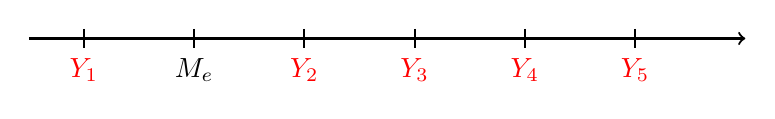
\begin{tikzpicture}[scale=7]
		\draw[->, thick] (-0.1,0) -- (1.2,0);
		\foreach \x/\xtext in {0/$\color{red}{Y_1}$,0.2/$M_e$,0.4/$\color{red}{Y_2}$,0.6/$\color{red}{Y_3}$,0.8/$\color{red}{Y_4}$,1.0/$\color{red}{Y_5}$}
		    \draw[thick] (\x,0.5pt) -- (\x,-0.5pt) node[below] {\xtext};
		\end{tikzpicture}
	\end{figure}
	La médiane $M_e$ de la population est prise en sandwich entre $Y_1$ et $Y_5$, si les deux premières statistiques d'ordre sont les seules statistiques de commande inférieures à la médiane $M_e$:
	\begin{figure}[H]
		\centering
		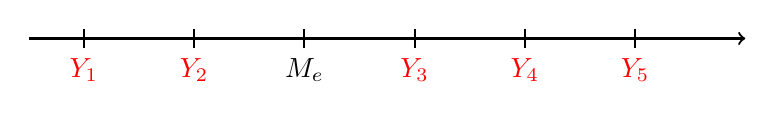
\begin{tikzpicture}[scale=7]
		\draw[->, thick] (-0.1,0) -- (1.2,0);
		\foreach \x/\xtext in {0/$\color{red}{Y_1}$,0.2/$\color{red}{Y_2}$,0.4/$M_e$,0.6/$\color{red}{Y_3}$,0.8/$\color{red}{Y_4}$,1.0/$\color{red}{Y_5}$}
		    \draw[thick] (\x,0.5pt) -- (\x,-0.5pt) node[below] {\xtext};
		\end{tikzpicture}
	\end{figure}
	La médiane $M_e$ de la population est prise en sandwich entre $Y_1$ et $Y_5$, si les trois premières statistiques d'ordre sont inférieures à la médiane $M_e$, et les statistiques de quatrième et cinquième ordre sont supérieures à $M_e$:
	\begin{figure}[H]
		\centering
		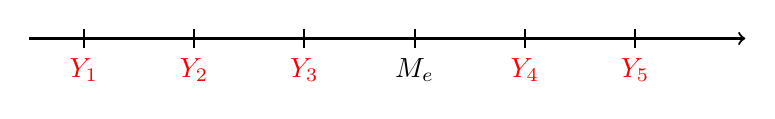
\begin{tikzpicture}[scale=7]
		\draw[->, thick] (-0.1,0) -- (1.2,0);
		\foreach \x/\xtext in {0/$\color{red}{Y_1}$,0.2/$\color{red}{Y_2}$,0.4/$\color{red}{Y_3}$,0.6/$M_e$,0.8/$\color{red}{Y_4}$,1.0/$\color{red}{Y_5}$}
		    \draw[thick] (\x,0.5pt) -- (\x,-0.5pt) node[below] {\xtext};
		\end{tikzpicture}
	\end{figure}
	Et, la médiane $M_e$ de la population est prise en sandwich entre $Y_1$ et $Y_5$, si la statistique de cinquième ordre est la seule statistique d'ordre supérieure à la médiane $M_e$:
	\begin{figure}[H]
		\centering
		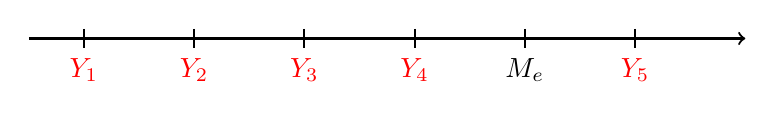
\begin{tikzpicture}[scale=7]
		\draw[->, thick] (-0.1,0) -- (1.2,0);
		\foreach \x/\xtext in {0/$\color{red}{Y_1}$,0.2/$\color{red}{Y_2}$,0.4/$\color{red}{Y_3}$,0.6/$\color{red}{Y_4}$,0.8/$M_e$,1.0/$\color{red}{Y_5}$}
		    \draw[thick] (\x,0.5pt) -- (\x,-0.5pt) node[below] {\xtext};
		\end{tikzpicture}
	\end{figure}
	Cela signifie que pour calculer la probabilité $P(Y_1 \leq M_e \leq Y_5)$, nous devons calculer la probabilité de chacun des événements ci-dessus. Maintenant, si nous désigner par $W$ le nombre de $X_i < M_e$, alors $W$ est une variable aléatoire binomiale avec $n$ essais mutuellement indépendants et probabilité de succès $p = P (X_i <M_e) = 0.5$  Et, en examinant les événements décrits ci-dessus, la probabilité souhaitée est calculée comme suit:
	
	La fonction de masse de probabilité binomiale (ou, alternativement, la table binomiale) rend le calcul simple:
	
	Ainsi, la probabilité que l'intervalle aléatoire $[Y1, Y5]$ contienne la médiane $M_e$ est de $0.9376$. Nous n'avons pas toujours autant de chance d'arriver à un coefficient de confiance décent dès notre premier essai. Parfois, nous devons réessayer en visant à obtenir un coefficient de confiance d'au moins $90\%$, mais aussi proche de $95\%$ que possible. Dans ce cas, le coefficient de confiance pour l'intervalle $[Y2, Y4]$ est:
	
	De toute évidence, nous ferions mieux de nous en tenir à l'intervalle $ [Y_1, Y_5] $ dans ce cas.
	
	Notez qu'en général nous avons alors:
	
	La méthode que nous avons apprise pour trouver un intervalle de confiance pour la médiane d'une distribution continue peut être facilement étendue afin que nous puissions trouver un intervalle de confiance pour tout centile $\pi_p$. La seule chose que nous devons changer est la probabilité de succès, c'est-à-dire que $X_i$ est inférieur à $\pi_p$:
	
	Ensuite, le coefficient de confiance exact est calculé comme avant en utilisant la distribution binomiale avec les paramètres $n$ et $p$:
	
	
	\paragraph{Test de la somme des rangs de Wilcoxon}\mbox{}\\\\
	L'idée du "\NewTerm{test de la somme des rangs de Wilcoxon}\index{test de la somme des rangs de Wilcoxon}\label{Wilcoxon rank sum test}" est la suivante: si nous collectons deux échantillons de mesure, et que nous stockons les valeurs dans l'ordre, l'alternance des $X_i$ (de taille $n_x$) et $Y_i$ (de taille $n_y$) devrait être assez stable si les deux lois de distribution  $F$ et $G$ d'échantillons suivent respectivement la même distribution de probabilité. C'est donc comme un "contrôle d'adéquation".
	
	Cela revient en fait à dire que l'hypothèse nulle est: \textit{La distribution des rangs dans les deux groupes est égale}.
	
	Formellement:
	
	En langage clair, l'hypothèse nulle est que la probabilité qu'une observation aléatoire du groupe $A$ dépasse l'observation appariée tirée du groupe $B$ est de moitié (c'est-à-dire qu'une observation aléatoire du groupe $A$ a autant de probabilité d'être supérieure que comme étant inférieure à son observation appariée dans le groupe $B$).
	
	La valeur pratique de ceci est difficile à voir, et donc dans de nombreux endroits, y compris les manuels de référence universitaire, l'hypothèse nulle est présentée comme les \og deux populations ont des médianes égales \fg{}. L'hypothèse nulle actuelle peut être exprimée comme l'hypothèse mentionnée avec la médiane, mais seulement sous l'hypothèse supplémentaire que les formes des distributions sont identiques dans chaque groupe!
	
	En d'autres termes, notre interprétation du test comme la comparaison des médianes des distributions exige le déplacement du paramètre de localisation uniquement. Comme cela est rarement vrai et jamais évalué, nous devrions probablement faire preuve d'une extrême prudence dans l'utilisation, et en particulier dans l'interprétation, du test de la somme des rangs de Wilcoxon.
	
	Il n'est donc pas comme le test d'adéquation du chi-carré de comparer des mesures à une loi théorique, mais à d'autres mesures d'une même loi hypothétique.
	
	\begin{tcolorbox}[title=Remarque,colframe=black,arc=10pt]
	Le test de la somme des rangs de Wilcoxon est un test non paramétrique, utilisé donc pour les "Tests de signification d'hypothèse nulle non paramétriques", car nous n'avons besoin d'aucune mesure de dispersion (ie variance) ou de localisation (ie moyenne) des variables aléatoires. De plus, il s'agit d'un test dit "robuste" dans le sens où il ne suppose pas la Normalité des données.
	\end{tcolorbox}	
	Prenons un exemple avant d'aborder l'aspect théorique. Voici deux échantillons de taille $10$ ($n_x = n_y$) de variables quantitatives:
	
	\begin{tcolorbox}[title=Remarque,colframe=black,arc=10pt]
	Le test de la somme des rangs de Wilcoxon peut très bien être utilisé pour les variables ordinales (mais seulement tant qu'elles sont dans un nombre acceptable). En règle générale, le test de la somme des rangs de Wilcoxon est également utilisé pour analyser les réponses aux enquêtes auprès des entreprises en utilisant une échelle de Likert en $7$ points.
	\end{tcolorbox}	
	Voici les statistiques d'ordre de l'échantillon de taille $20$ ($N=n_x+n_y$) regroupés et ordonnés (les $10$ valeurs du premier échantillon sont soulignées):
	
	Les valeurs du premier échantillon $X$ (nommé "\NewTerm{valeurs de traitement}\index{valeurs de traitement}") dans cet exemple semblent être plus petites que celles du deuxième échantillon $Y$ (nommé "\NewTerm{valeurs de contrôle}\index{valeurs de contrôle}") que nous représentons souvent dans un diagramme comme suit (en trichant un peu avec Microsoft Excel 11.8346):
	\begin{figure}[H]
		\centering
		\includegraphics{img/arithmetics/wilcoxon_rank_sum_test_ordered_values.jpg}
		\caption[]{Comparaison des valeurs ordonnées de deux échantillons dans Microsoft Excel 11.8346}
	\end{figure}
	\begin{tcolorbox}[title=Remarque,colframe=black,arc=10pt]
	Vous devez faire attention au test de Wilcoxon que nous étudions ici et au test de Kruskal-Wallis que nous verrons plus tard. En effet, beaucoup de gens pensent que parce qu'ils ne sont pas paramétriques, ils n'ont aucune hypothèse ... Cependant, comme nous le savons, c'est faux !!! Un test non paramétrique est en effet indépendant des paramètres de distribution mais il peut y avoir d'autres hypothèses. Dans le cas du test de Wilcoxon et du test de Kruskal-Wallis, l'hypothèse est (bien évidemment ...) que les paramètres d'échelle entre les deux échantillons sont égaux (sinon ce serait un non-sens de comparer deux choses que l'on sait déjà comme n'étant pas comparables!).
	\end{tcolorbox}	
	L'idée est alors de savoir si cette tendance est statistiquement significative? C'est-à-dire si nous avons une différence du genre $F<G$ entre leurs lois de distribution respectives:
	\begin{figure}[H]
		\centering
		\includegraphics{img/arithmetics/wilcoxon_rank_sum_distribution_comparison.jpg}
		\caption[]{Exemple générique de comparaison de deux distributions dans Microsoft Excel 11.8346}
	\end{figure}
	ou si elles peuvent être considérés comme identiques. Pour cela, nous devons examiner le concept de "\NewTerm{rang}\index{rang}":
	
	\textbf{Définition (\#\mydef):} Étant donné un échantillon aléatoire $X_1,X_2,...,X_n$ de taille $n$ de toute loi statistique continue, nous notons $R_i$ le rang des $X_i$ ordonnés dans un échantillon de population. Le rang $i$ est un entier non nul strictement positif et compris entre $1$ et $n$.
	
	\begin{tcolorbox}[colframe=black,colback=white,sharp corners]
	\textbf{{\Large \ding{45}}Exemple:}\\\\
	Dans:
	
	Nous avons respectivement les "statistiques d'ordre" suivantes:
	
	Une fois le concept de "rang" défini et calculé, regardons la somme dans le cadre de notre exemple avec deux échantillons:
	
	Le somme des  rangs notée traditionnellement $W_x$ ($W$ pour Wilcoxon) pour le premier échantillon est donc:
	
	et pour le deuxième échantillon:
	
	\end{tcolorbox}
	Les valeurs $W_x,W_y$ sont nommées "\NewTerm{statistiques de Wilcoxon}\index{statistique de Wilcoxon}".
	
	On voit donc déjà qu'il existe bien une différence qui semble a priori significative en termes de classement entre les deux échantillons. Le problème reste de construire un outil mathématique rigoureux pour inférer un fait avec une certaine certitude.
	
	Pour cela, introduisons d'abord la moyenne des rangs en utilisant le résultat présenté dans la section Séquences et Séries en ne considérant qu'un seul échantillon:
	
	En calculant cela, nous remarquons rapidement qu'il s'agit de l'espérance la la distribution discrète uniforme que nous avions étudié plus haut dans cette section pour une variable aléatoire discrète avec des valeurs comprises entre $1$ et $n$, ce qui est exactement la définition du rang! Ainsi, nous avons le rang qui aura comme valeur pour la moyenne et la variance pour l'ensemble de la population:
	
	Pour ceux qui trouvent cette analogie discutable, nous donnons juste en dessous la preuve de la variance en utilisant la relation de Huygens et la somme des carrés d'entiers positifs prouvée dans la section Séquences et Séries:
	
	Mais évidemment pour un seul échantillon cela n'a aucun intérêt! Reprenons nos deux séries $X_i,Y_i$ respectivement de taille égale $n_x=10,n_y=10$ sans distinction:
	
	On a alors les indicateurs statistiques de rangs sans distinction (il faut se rappeler que l'on ne sait toujours pas à ce niveau du développement mathématique si cela sera utile ou non):
	
	et les indicateurs statistiques des rangs mais cette fois avec distinction:
	
	Nous avons alors les indicateurs statistiques de localisation suivants:
	
	Ces calculs maintenant effectués, nous n'avons rien de concret encore rigoureux concernant le test de la somme des rangs de Wilcoxon qui a pour but, pour rappel, de vérifier si les deux échantillons suivent la même loi ou non (et ont donc les mêmes moments tels l'espérance, la variance, la médiane, etc.).
	
	Pour avancer, considérons les $n_x$ valeurs de l'échantillon $X$. On sait (\SeeChapter{voir section Probabilités page \pageref{binomial coefficient}}) alors qu'il y a:
	
	nombre d'arrangements possibles des $X_i$ dans la population des échantillons et si le test de la somme des rangs de Wilcoxon est vérifié (c'est-à-dire que les lois de probabilité sont les mêmes pour les deux échantillons), les divers arrangements devraient être également probables.
	
	Par exemple, si nous prenons $2$ échantillons avec respectivement chacun $2$  mesures ($2$ variables aléatoires de traitement et $2$ variables aléatoires de contrôle), nous avons:
	
	arrangements tous différents:
	
	Mais ... malheureusement ... ce n'est pas ce que nous voulons dans notre cas car nous aimerions déjà pouvoir distinguer les deux échantillons et aussi ne pas prendre en compte les arrangements qui consistent uniquement en une permutation des variables du même échantillon. On a alors (\SeeChapter{voir section Probabilités page \pageref {binomial coefficient}}):
	
	combinaisons possibles! En effet, avec deux échantillons ayant deux variables de traitement ($X$) et deux variables de contrôle ($Y$), nous avons ($W_S$ est la somme des rangs de la dernière colonne):
	\begin{table}[H]
		\centering
		\definecolor{gris}{gray}{0.85}
				\begin{tabular}{|c|c|c|}
					\hline
	\multicolumn{1}{c}{\cellcolor{black!30}\pbox{20cm}{\textbf{Rangs possibles} \\ \textbf{(contrôles)}}} & \multicolumn{1}{c}{\cellcolor{black!30}\pbox{20cm}{\textbf{Rangs possibles} \\ \textbf{(traitements)}}} & \multicolumn{1}{c}{\cellcolor{black!30}$W_S$} \\ \hline
			$1,2$ & $3,4$ & $7$\\ 
			$1,3$ & $2,4$ & $6$\\ 
			$1,4$ & $2,3$ & $5$\\ \hline
			$2,3$ & $1,4$ & $4$\\ 
			$2,4$ & $1,3$ & $4$\\ \hline
			$3,4$ & $1,2$ & $3$\\ \hline
		\end{tabular}
		\caption[]{Représentation par rangs de $2$ variables de traitement et de contrôle}
	\end{table}
	Si l'hypothèse nulle du test de la somme des rangs de Wilcoxon n'est pas rejetée, les classements des $6$ sont également probables. Nous concluons le tableau suivant:
	\begin{table}[H]
		\centering
		\definecolor{gris}{gray}{0.85}
		\begin{tabular}{|c|c|c|c|c|c|}
			\hline
\multicolumn{1}{c}{\cellcolor{black!30}\pbox{20cm}{\textbf{Valeur de $W_S$} }} & \multicolumn{1}{c}{\cellcolor{black!30}\pbox{20cm}{$3$}} & \multicolumn{1}{c}{\cellcolor{black!30}\pbox{20cm}{$4$}} & \multicolumn{1}{c}{\cellcolor{black!30}\pbox{20cm}{$5$}} & \multicolumn{1}{c}{\cellcolor{black!30}\pbox{20cm}{$6$}} & \multicolumn{1}{c}{\cellcolor{black!30}\pbox{20cm}{$7$}}\\ \hline
	\multicolumn{1}{c}{\cellcolor{black!30}\pbox{20cm}{\textbf{Probabilité}}} & $\dfrac{1}{6}$ & $\dfrac{1}{6}$ & $\dfrac{2}{6}$ & $\dfrac{1}{6}$ & $\dfrac{1}{6}$\\ 
	\multicolumn{1}{c}{\cellcolor{black!30}\pbox{20cm}{\textbf{Cumul}}} & $\dfrac{1}{6}$ & $\dfrac{2}{6}$ & $\dfrac{4}{6}$ & $\dfrac{5}{6}$ & $\dfrac{6}{6}$\\ \hline
		\end{tabular}
		\caption[]{Probabilités associées au test de la somme des rangs de Wilcoxon}
	\end{table}
	Ce tableau étant construit, supposons que l'on observe pour la somme des rangs des variables de traitement: $W_S = 7$. Le seuil d'un test unilatéral donnerait alors conformément au tableau ci-dessus:
	
	ou si nous obtenons $W_S=3$:
	
	On rejetterait donc l'hypothèse nulle d'une distribution identique entre les deux échantillons à toute limite supérieure (ou inférieure, respectivement) fixée à l'avance par la politique du laboratoire ... en test unilatéral ou bilatéral (raison pour laquelle certains logiciels statistiques donnent des valeurs de test unilatérales + valeurs de test bilatérales en même temps).
	
	Deux choses très importantes que vous devez noter pour ce qui va suivre sont les suivantes:
	\begin{enumerate}
		\item D'abord dans la construction du tableau ci-dessus (où nous reprenons la première partie ici):
		\begin{table}[H]
			\begin{center}
				\definecolor{gris}{gray}{0.85}
					\begin{tabular}{|c|c|c|c|c|c|}
						\hline
		\multicolumn{1}{c}{\cellcolor{black!30}\pbox{20cm}{\textbf{Valeurs de $W_S$} }} & \multicolumn{1}{c}{\cellcolor{black!30}\pbox{20cm}{$3$}} & \multicolumn{1}{c}{\cellcolor{black!30}\pbox{20cm}{$4$}} & \multicolumn{1}{c}{\cellcolor{black!30}\pbox{20cm}{$5$}} & \multicolumn{1}{c}{\cellcolor{black!30}\pbox{20cm}{$6$}} & \multicolumn{1}{c}{\cellcolor{black!30}\pbox{20cm}{$7$}}\\ \hline
				\multicolumn{1}{c}{\cellcolor{black!30}\pbox{20cm}{\textbf{Probabilité}}} & $\dfrac{1}{6}$ & $\dfrac{1}{6}$ & $\dfrac{2}{6}$ & $\dfrac{1}{6}$ & $\dfrac{1}{6}$\\ \hline
			\end{tabular}
			\end{center}
		\end{table}
		on voit qu'il y a une symétrie à la valeur $5$, ce qui signifie que la loi $W_S$ est symétrique dans ce cas particulier. Mais si nous prenons un autre exemple avec deux échantillons comprenant respectivement deux variables de contrôle et trois de traitements (deux variables aléatoires) nous aurions:
		\begin{table}[H]
			\begin{center}
				\definecolor{gris}{gray}{0.85}
					\begin{tabular}{|c|c|c|c|c|c|c|c|}
						\hline
		\multicolumn{1}{c}{\cellcolor{black!30}\pbox{20cm}{\textbf{Valeurs de $W_S$} }} & \multicolumn{1}{c}{\cellcolor{black!30}\pbox{20cm}{$6$}} & \multicolumn{1}{c}{\cellcolor{black!30}\pbox{20cm}{$7$}} & \multicolumn{1}{c}{\cellcolor{black!30}\pbox{20cm}{$8$}} & \multicolumn{1}{c}{\cellcolor{black!30}\pbox{20cm}{$9$}} & \multicolumn{1}{c}{\cellcolor{black!30}\pbox{20cm}{$10$}} & \multicolumn{1}{c}{\cellcolor{black!30}\pbox{20cm}{$11$}} & \multicolumn{1}{c}{\cellcolor{black!30}\pbox{20cm}{$12$}}\\ \hline
				\multicolumn{1}{c}{\cellcolor{black!30}\pbox{20cm}{\textbf{Probabilité}}} & $\dfrac{1}{10}$ & $\dfrac{1}{10}$ & $\dfrac{2}{10}$ & $\dfrac{2}{10}$ & $\dfrac{2}{10}$ & $\dfrac{1}{10}$ & $\dfrac{1}{10}$\\  \hline
			\end{tabular}
			\end{center}
		\end{table}
		le lecteur peut vérifier que quel que soit le nombre d'échantillons et le nombre de variables et de traitement de contrôle, le tableau de probabilité ci-dessus est toujours équilibré (enfin il y a une preuve mathématique de cela mais je la trouve inélégante...). Mais en fait c'est assez intuitif, comme les combinaisons $C_{n_x}^{n_x+n_y}$ sont indépendantes du fait que les rangs sont triés par ordre croissant ou décroissant, il faut donc qu'il y ait une symétrie.
		
		\item Deuxièmement, les valeurs des variables mesurées n'entrent pas en compte dans cette statistique paramétrique mais uniquement les valeurs tabulées des rangs avec leurs probabilités associées. En effet, comme vous l'avez peut-être remarqué, nous n'avions pas besoin de valeurs explicites des variables aléatoires pour construire le tableau ci-dessus!
	\end{enumerate}
	
	Maintenant, sachant que la loi $ W_S $ est symétrique et discrète nous aimerions calculer son espérance.
	
	La plus petite valeur possible de $W_S$ suppose qu'elle se trouve dans l'échantillon $X$ (les algorithmes informatiques déterminent automatiquement dans quel échantillon mais de toute façon en pratique, les échantillons ont presque toujours la même taille):
	
	La plus grande valeur possible est naturellement (rappelons que $N=n_x+n_y$):
	
	L'espérance de la somme des rangs de l'un des deux échantillons est alors:
	
	Alors finalement:
	
	Pour calculer la variance, qui nous sera utile pour faire si nécessaire une approximation que nous verrons plus loin, apparaît (malheureusement) la covariance car la connaissance des rangs donne des informations partielles sur les autres rangs. Nous avons donc:
	
	Nous savons déjà avec ce que nous venons de prouver ci-dessus que:
	
	Le problème reste le terme avec la covariance. Pour son calcul il existe des techniques rigoureuses en plusieurs pages et ... et aussi... un astuce bien plus courte. L'astuce consiste à utiliser la variable de classement global que nous notons $T_i$ avec $i=1...n+m$. Comme la somme des $T_i$ est une constante, alors nous avons:
	
	Il vient alors:
	
	On peut alors reprendre le calcul initial en remplaçant les covariances par leur expression, la dernière relation obtenue pour les covariances calculées sur le $T_i$ s'appliquant aussi (ce qui n'est pas forcément intuitif ... mais l'astuce fonctionne) aux $ R_i $:
	
	Finalement:
	
	C'est le même résultat que la méthodologie rigoureuse que l'on retrouve dans quelques rares manuels de référence.
	\begin{tcolorbox}[colframe=black,colback=white,sharp corners]
	\textbf{{\Large \ding{45}}Exemple:}\\\\
	Passons à un cas pratique pour le cas exact. Considérons donc $2$ échantillons  ayant $2$ variables de traitements $(X)$ et $2$ variables de contrôle $(Y)$ (c'est un peu simpliste et absurde comme exemple mais cela facilite l'aspect pédagogique ...) nous avons:
	
	Ainsi (la variable de traitement a donc les rangs $1$ et $3$ ce qui fait une somme des rang de $4$):
	
	Dès lors:
	
	Nous avons le tableau suivant comme nous l'avons montré ci-dessus:
	\begin{table}[H]
			\begin{center}
				\definecolor{gris}{gray}{0.85}
					\begin{tabular}{|c|c|c|c|c|c|}
						\hline
		\multicolumn{1}{c}{\cellcolor{black!30}\pbox{20cm}{\textbf{Valeurs de $W_S$} }} & \multicolumn{1}{c}{\cellcolor{black!30}\pbox{20cm}{$3$}} & \multicolumn{1}{c}{\cellcolor{black!30}\pbox{20cm}{$4$}} & \multicolumn{1}{c}{\cellcolor{black!30}\pbox{20cm}{$5$}} & \multicolumn{1}{c}{\cellcolor{black!30}\pbox{20cm}{$6$}} & \multicolumn{1}{c}{\cellcolor{black!30}\pbox{20cm}{$7$}}\\ \hline
				\multicolumn{1}{c}{\cellcolor{black!30}\pbox{20cm}{\textbf{Probabilité}}} & $\dfrac{1}{6}$ & $\dfrac{1}{6}$ & $\dfrac{2}{6}$ & $\dfrac{1}{6}$ & $\dfrac{1}{6}$\\  \hline
			\end{tabular}
			\end{center}
	\end{table}
	avec dans le cas présent:
	
	Si nous choisissons le seuil de confiance traditionnel à $5\%$ en bilatéral, nous avons selon le tableau ci-dessus que:
	
	Donc en d'autres termes nous voyons qu'il y a:
	\end{tcolorbox}
	
	\pagebreak
	\begin{tcolorbox}[colframe=black,colback=white,sharp corners]
	
	de probabilité cumulée que equationsoit compris entre $3$ et $7$ (la barre au-dessus du $6$ signifie pour rappel que ce chiffre se répète à l'infini). Donc forcément $4$ est compris dans l'intervalle bilatéral du $95\%$... et nous pouvons accepter l'hypothèse comme quoi les deux échantillons ne sont pas différents. La $p$-valeur correspondante en bilatéral est donc la moitié de $33.\bar{3}\%$.\\
	
	\begin{tcolorbox}[title=Remarque,colframe=black,arc=10pt]
	Au fait si nous voulions faire un exemple calculatoire manuel intéressant en jouant avec un seuil bilatéral de $5\%$ (soit de $2.5\%$ de chaque côté) il faudrait au moins $2$ échantillons avec $4$ variables aléatoires, soit $70$ combinaisons de rangs possibles. En-dessous de $4$ variables aléatoires par échantillons, il est évident que le test bilatéral à seuil de $95\%$ sera tel qu'on ne rejettera jamais l'hypothèse d'égalité...
	\end{tcolorbox}
	\end{tcolorbox}
	Si la taille des deux échantillons est assez grande (la majorité des praticiens considérent que chaque échantillon doit avoir au moins $20$ individus), il a été montré par simulations que nous pouvons faire l'approximation (utilisée par beaucoup de logiciels de statistiques):
	
	bien évidemment en déterminant ensuite toujours la $p$-valeur en bilatéral. Avec l'exemple précédent (n'ayant que $4$ individus au total), nous avons donc:
	
	Ce qui correspondant à une probabilité cumulée de $21.93\%$. Donc la $p$-valeur correspondante en bilatéral est d'environ $(1-22)\cong 44\%$  (à comparer à la valeur d'environ $33\%$ avec le cas exact).
	
	\paragraph{Test de la somme des rangs de Mann-Whitney}\mbox{}\\\\
	Le "\NewTerm{test de la somme des rangs de Mann-Withney}\index{test de la somme des rangs de Mann-Withney}" est au fait un test d'ajustement non-paramétrique très simple qui se déduit du test de la somme des rangs de Wilcoxon. Par ailleurs il en est inspiré à un tel point que nous l'appelons parfois dans l'industrie le \NewTerm{test de Wilcoxon-Mann-Withney}\index{test de Wilcoxon-Mann-Withney}" ou "\NewTerm{test d'ajustement de Wilcoxon-Mann-Withney}\index{test d'ajustement de Wilcoxon-Mann-Withney}" ou encore "\NewTerm{Mtest MWW}" (sans spécifier à chaque fois qu'il repose sur la somme des rangs).
	
	Le but de ce test, identiquement au test de la somme des rangs de Wilcoxon, est de trouver un moyen de vérifier que deux échantillons indépendants non nécessairement de même taille sont issus d'une même loi ou non (in extenso sont issus d'une même population ou non) mais avec une approche différente!
	
	\begin{tcolorbox}[title=Remarque,colframe=black,arc=10pt]
	Au même titre que le test de la somme des rangs de Wilcoxon, le test de la somme des rangs de Mann-Withney peut tout à fait être utilisé pour des variables ordinales (donc catégorielles mais à condition qu'elles soient en un nombre acceptable).
	\end{tcolorbox}
	
	Certains logiciels par ailleurs portent les choses à confusion car ils proposent le test de la somme des rangs de Wilcoxon sous le nom de test de de Mann-Withney... et inversement... et de plus n'indiquent pas ou ne proposent pas toujours le choix entre la version exacte ou approximative... Et en plus le test de la somme des rangs de Wilcoxon et celui de la somme des rangs signés que nous verrons plus loin n'est pas différencié.... donc attention! C'est typiquement un problème dont la source est l'absence d'une norme ISO définissant la terminologie et les options qui doivent être disponibles...

	Pour voir en quoi ce test consiste, construisons le tableau de rangs utilisant deux échantillons comprenant deux variables de contrôle et trois variables de traitement, nous avons alors:
	\begin{table}[H]
		\centering
		\definecolor{gris}{gray}{0.85}
		\begin{tabular}{|c|c|c|}
		\hline
\multicolumn{1}{c}{\cellcolor{black!30}\pbox{20cm}{\textbf{Rangs possibles} \\ \textbf{(Contrôles)}}} & \multicolumn{1}{c}{\cellcolor{black!30}\pbox{20cm}{\textbf{Rangs possibles} \\ \textbf{(Traitements)}}} & \multicolumn{1}{c}{\cellcolor{black!30}$W_S$} \\ \hline
		$1,2$ & $3,4,5$ & $12$\\ 
		$1,3$ & $2,4,5$ & $11$\\
		$1,4$ & $2,3,5$ & $10$\\  
		$1,5$ & $2,3,4$ & $9$\\ \hline
		$2,3$ & $1,4,5$ & $10$\\
		$2,4$ & $1,3,5$ & $9$\\  
		$2,5$ & $1,3,4$ & $8$\\ \hline
		$3,4$ & $1,2,5$ & $8$\\ 
		$3,5$ & $1,2,4$ & $7$\\ \hline
		$4,5$ & $1,2,3$ & $6$\\ \hline
		\end{tabular}
		\caption[]{Représentation des rangs de 3 variables de traitement et 2 de contrôle}
	\end{table}
	Dont nous déduisons le tableau suivant:
	\begin{table}[H]
		\centering
		\definecolor{gris}{gray}{0.85}
		\begin{tabular}{|c|c|c|c|c|c|c|c|}
		\hline
	\multicolumn{1}{c}{\cellcolor{black!30}\pbox{20cm}{\textbf{Valeurs de $W_S$} }} & \multicolumn{1}{c}{\cellcolor{black!30}\pbox{20cm}{$6$}} & \multicolumn{1}{c}{\cellcolor{black!30}\pbox{20cm}{$7$}} & \multicolumn{1}{c}{\cellcolor{black!30}\pbox{20cm}{$8$}} & \multicolumn{1}{c}{\cellcolor{black!30}\pbox{20cm}{$9$}} & \multicolumn{1}{c}{\cellcolor{black!30}\pbox{20cm}{$10$}} & \multicolumn{1}{c}{\cellcolor{black!30}\pbox{20cm}{$11$}} & \multicolumn{1}{c}{\cellcolor{black!30}\pbox{20cm}{$12$}}\\ \hline
			\multicolumn{1}{c}{\cellcolor{black!30}\pbox{20cm}{\textbf{Probabilités}}} & $\dfrac{1}{10}$ & $\dfrac{1}{10}$ & $\dfrac{2}{10}$ & $\dfrac{2}{10}$ & $\dfrac{2}{10}$ & $\dfrac{1}{10}$ & $\dfrac{1}{10}$\\  \hline
		\end{tabular}
	\end{table}
	Maintenant imaginons que nous ayons une autre expérience à analyser utilisant deux échantillons comprenant $3$ variables de contrôle et $2$ variables de traitement (le symétrique du précédent donc!), nous avons alors:
	\begin{table}[H]
		\centering
		\definecolor{gris}{gray}{0.85}
				\begin{tabular}{|c|c|c|}
					\hline
	\multicolumn{1}{c}{\cellcolor{black!30}\pbox{20cm}{\textbf{Rangs possibles} \\ \textbf{(Contrôles)}}} & \multicolumn{1}{c}{\cellcolor{black!30}\pbox{20cm}{\textbf{Rangs possibles} \\ \textbf{(Traitements)}}} & \multicolumn{1}{c}{\cellcolor{black!30}$W_S$} \\ \hline
			$3,4,5$ & $1,2$ & $3$\\ 
			$2,4,5$ & $1,3$ & $4$\\
			$2,3,5$ & $1,4$ & $5$\\  
			$2,3,4$ & $1,5$ & $6$\\ \hline
			$1,4,5$ & $2,3$ & $5$\\
			$1,3,5$ & $2,4$ & $6$\\  
			$1,3,4$ & $2,5$ & $7$\\ \hline
			$1,2,5$ & $3,4$ & $7$\\ 
			$1,2,4$ & $3,5$ & $8$\\ \hline
			$1,2,3$ & $4,5$ & $9$\\ \hline
		\end{tabular}
		\caption[]{Représentation des rangs de 2 variables de traitement et 3 de contrôle}
	\end{table}
	Dont nous déduisons le tableau suivant (le lecteur remarquera que c'est exactement le même que le précédent en ce qui concerne les probabilités!!):
	\begin{table}[H]
		\centering
		\definecolor{gris}{gray}{0.85}
		\begin{tabular}{|c|c|c|c|c|c|c|c|}
		\hline
		\multicolumn{1}{c}{\cellcolor{black!30}\pbox{20cm}{\textbf{Valeurs de $W_S$} }} & \multicolumn{1}{c}{\cellcolor{black!30}\pbox{20cm}{$3$}} & \multicolumn{1}{c}{\cellcolor{black!30}\pbox{20cm}{$4$}} & \multicolumn{1}{c}{\cellcolor{black!30}\pbox{20cm}{$5$}} & \multicolumn{1}{c}{\cellcolor{black!30}\pbox{20cm}{$6$}} & \multicolumn{1}{c}{\cellcolor{black!30}\pbox{20cm}{$7$}} & \multicolumn{1}{c}{\cellcolor{black!30}\pbox{20cm}{$8$}} & \multicolumn{1}{c}{\cellcolor{black!30}\pbox{20cm}{$9$}}\\ \hline
			\multicolumn{1}{c}{\cellcolor{black!30}\pbox{20cm}{\textbf{Probabilité}}} & $\dfrac{1}{10}$ & $\dfrac{1}{10}$ & $\dfrac{2}{10}$ & $\dfrac{2}{10}$ & $\dfrac{2}{10}$ & $\dfrac{1}{10}$ & $\dfrac{1}{10}$\\  \hline
		\end{tabular}
	\end{table}
	Eh bien l'idée du test de Mann-Withney est très simple. Plutôt que de tabuler des situations symétriques, il suffit de soustraire à chaque valeur de $W_S$, la valeur  $W_{S,\min}$ afin que chaque tableau soit identique et qu'un des deux seul soit utile. Voyons cela d'abord avec le premier tableau:
	\begin{table}[H]
		\centering
		\definecolor{gris}{gray}{0.85}
		\begin{tabular}{|c|c|c|}
					\hline
	\multicolumn{1}{c}{\cellcolor{black!30}\pbox{20cm}{\textbf{Rangs possibles} \\ \textbf{(Contrôles)}}} & \multicolumn{1}{c}{\cellcolor{black!30}\pbox{20cm}{\textbf{Rangs possibles} \\ \textbf{(Traitements)}}} & \multicolumn{1}{c}{\cellcolor{black!30}$W_s-\dfrac{1}{2}n_x(n_x+1)
$} \\ \hline
			$1,2$ & $3,4,5$ & $6$\\ 
			$1,3$ & $2,4,5$ & $5$\\
			$1,4$ & $2,3,5$ & $4$\\  
			$1,5$ & $2,3,4$ & $3$\\ \hline
			$2,3$ & $1,4,5$ & $4$\\
			$2,4$ & $1,3,5$ & $3$\\  
			$2,5$ & $1,3,4$ & $2$\\ \hline
			$3,4$ & $1,2,5$ & $2$\\ 
			$3,5$ & $1,2,4$ & $1$\\ \hline
			$4,5$ & $1,2,3$ & $0$\\ \hline
		\end{tabular}
		\caption[]{Symétrisation ($2$ contrôles/$3$ traitements)}
	\end{table}
	Dont nous déduisons le tableau suivant:
	\begin{table}[H]
		\centering
		\definecolor{gris}{gray}{0.85}
				\begin{tabular}{|c|c|c|c|c|c|c|c|}
					\hline
	\multicolumn{1}{c}{\cellcolor{black!30}\pbox{20cm}{\textbf{Valeurs de $W_{XY}$} }} & \multicolumn{1}{c}{\cellcolor{black!30}\pbox{20cm}{$0$}} & \multicolumn{1}{c}{\cellcolor{black!30}\pbox{20cm}{$1$}} & \multicolumn{1}{c}{\cellcolor{black!30}\pbox{20cm}{$2$}} & \multicolumn{1}{c}{\cellcolor{black!30}\pbox{20cm}{$3$}} & \multicolumn{1}{c}{\cellcolor{black!30}\pbox{20cm}{$4$}} & \multicolumn{1}{c}{\cellcolor{black!30}\pbox{20cm}{$5$}} & \multicolumn{1}{c}{\cellcolor{black!30}\pbox{20cm}{$6$}}\\ \hline
			\multicolumn{1}{c}{\cellcolor{black!30}\pbox{20cm}{\textbf{Probabilité}}} & $\dfrac{1}{10}$ & $\dfrac{1}{10}$ & $\dfrac{2}{10}$ & $\dfrac{2}{10}$ & $\dfrac{2}{10}$ & $\dfrac{1}{10}$ & $\dfrac{1}{10}$\\  \hline
		\end{tabular}
	\end{table}
	Maintenant imaginons que nous ayons une autre expérience à analyser utilisant deux échantillons comprenant $3$ variables de contrôle et $2$ variables de traitement (le symétrique du précédent donc!), nous avons alors:
	\begin{table}[H]
		\centering
		\definecolor{gris}{gray}{0.85}
			\begin{tabular}{|c|c|c|}
			\hline
	\multicolumn{1}{c}{\cellcolor{black!30}\pbox{20cm}{\textbf{Rangs possibles} \\ \textbf{(Contrôles)}}} & \multicolumn{1}{c}{\cellcolor{black!30}\pbox{20cm}{\textbf{Rangs possibles} \\ \textbf{(Traitements)}}} & \multicolumn{1}{c}{\cellcolor{black!30}$W_s-\dfrac{1}{2}n_x(n_x+1)
$} \\ \hline
			$3,4,5$ & $1,2$ & $0$\\ 
			$2,4,5$ & $1,3$ & $1$\\
			$2,3,5$ & $1,4$ & $2$\\  
			$2,3,4$ & $1,5$ & $3$\\ \hline
			$1,4,5$ & $2,3$ & $2$\\
			$1,3,5$ & $2,4$ & $3$\\  
			$1,3,4$ & $2,5$ & $4$\\ \hline
			$1,2,5$ & $3,4$ & $4$\\ 
			$1,2,4$ & $3,5$ & $5$\\ \hline
			$1,2,3$ & $4,5$ & $6$\\ \hline
		\end{tabular}
		\caption[]{Symétrisation ($2$ contrôles/$2$ traitements)}
	\end{table}
	Dont nous déduisons cette fois-ci exactement le même tableau que précédemment:
	\begin{table}[H]
		\centering
		\definecolor{gris}{gray}{0.85}
		\begin{tabular}{|c|c|c|c|c|c|c|c|}
			\hline
			\multicolumn{1}{c}{\cellcolor{black!30}\pbox{20cm}{\textbf{Valeurs de $W_{YX}$} }} & \multicolumn{1}{c}{\cellcolor{black!30}\pbox{20cm}{$0$}} & \multicolumn{1}{c}{\cellcolor{black!30}\pbox{20cm}{$1$}} & \multicolumn{1}{c}{\cellcolor{black!30}\pbox{20cm}{$2$}} & \multicolumn{1}{c}{\cellcolor{black!30}\pbox{20cm}{$3$}} & \multicolumn{1}{c}{\cellcolor{black!30}\pbox{20cm}{$4$}} & \multicolumn{1}{c}{\cellcolor{black!30}\pbox{20cm}{$5$}} & \multicolumn{1}{c}{\cellcolor{black!30}\pbox{20cm}{$6$}}\\ \hline
			\multicolumn{1}{c}{\cellcolor{black!30}\pbox{20cm}{\textbf{Probabilité}}} & $\dfrac{1}{10}$ & $\dfrac{1}{10}$ & $\dfrac{2}{10}$ & $\dfrac{2}{10}$ & $\dfrac{2}{10}$ & $\dfrac{1}{10}$ & $\dfrac{1}{10}$\\  \hline
		\end{tabular}
	\end{table}
	raison pour laquelle la littérature mentionne qu'on peut prendre celui que l'on veut!
	
	Donc pour résumer, la variante de Mann-Whitney (dans le cas concret ici présent il s'agit de la variante dite "\NewTerm{variante exacte de Mann-Whitney}\index{variante exacte de Mann-Whitney}") consiste à tabuler pour les situations symétriques une variable notée $W_{XY}$ définie naturellement par:
	
	Notée aussi très souvent dans la littérature:
	
	car alors $W_{XY}\in \left\lbrace 0,1,2,...\right\rbrace$ et donc:
	
	Dans les tables que l'on peut trouver dans les livres, les probabilités sont données avec la valeur normalisée de $U$. Ainsi, si nous reprenons notre exemple précédent mais avec les notations d'usage dans la pratique ($U$ au lieu de $W_{YX}$):
	\begin{table}[H]
		\centering
		\definecolor{gris}{gray}{0.85}
		\begin{tabular}{|c|c|c|c|c|c|c|c|}
			\hline
			\multicolumn{1}{c}{\cellcolor{black!30}\pbox{20cm}{\textbf{Valeurs de $U$} }} & \multicolumn{1}{c}{\cellcolor{black!30}\pbox{20cm}{$0$}} & \multicolumn{1}{c}{\cellcolor{black!30}\pbox{20cm}{$1$}} & \multicolumn{1}{c}{\cellcolor{black!30}\pbox{20cm}{$2$}} & \multicolumn{1}{c}{\cellcolor{black!30}\pbox{20cm}{$3$}} & \multicolumn{1}{c}{\cellcolor{black!30}\pbox{20cm}{$4$}} & \multicolumn{1}{c}{\cellcolor{black!30}\pbox{20cm}{$5$}} & \multicolumn{1}{c}{\cellcolor{black!30}\pbox{20cm}{$6$}}\\ \hline
			\multicolumn{1}{c}{\cellcolor{black!30}\pbox{20cm}{\textbf{Probabilité}}} & $\dfrac{1}{10}$ & $\dfrac{1}{10}$ & $\dfrac{2}{10}$ & $\dfrac{2}{10}$ & $\dfrac{2}{10}$ & $\dfrac{1}{10}$ & $\dfrac{1}{10}$\\  \hline
		\end{tabular}
	\end{table}
	Nous voyons que la probabilité cumulée que $U=2$ est de $0.4$. La table précédente se trouve dans la littérature parfois sous la forme suivante:
	\begin{table}[H]
		\centering
		\definecolor{gris}{gray}{0.85}
		\begin{tabular}{ |c|c|c|c| }
			\hline
			\multicolumn{4}{ |c| }{\cellcolor{black!30}\pbox{20cm}{Facteur $n_2=3$}} \\
			\hline
			$U/n_1$ & $1$ & $2$ & $3$ \\ \hline
			 $0$ & $0.250$ & $0.100$ & $0.050$ \\ \hline
			 $1$ & $0.500$ & $0.200$ & $0.100$ \\ \hline
			 $2$ & $0.750$ & \textbf{0.400} & $0.200$ \\ \hline
			 $3$ & $1$ & $0.600$ & $0.350$ \\ \hline
			 $4$ &  & $0.800$ & $0.500$ \\ \hline
			 $5$ &  & $0.900$ & $0.650$ \\ \hline
			 $6$ &  & $1$ & $\ldots$ \\ \hline
		\end{tabular}
		\caption[]{Représentation classique du test de Mann-Whitney}
	\end{table}
	où nous avons mis en rouge la colonne correspondant à notre exemple  ($U=2,n_1=2,n_2=3$).
	
	Ensuite il convient au praticien de choisir avec ces tableaux s'il souhaite faire un test bilatéral ou unilatéral.
	
	\begin{tcolorbox}[title=Remarques,colframe=black,arc=10pt]
	\textbf{R1.} Il est important de se rappeler que nous avons démontré par l'exemple que nous pouvons aussi bien prendre:
	
	que:
	
	puisqu'ils génèrent les mêmes tableaux!\\
	
	\textbf{R2.} $W_{XY}$ est traditionnellement noté $U$ par les praticiens comme nous l'avons vu, d'où le fait que l'on retrouve dans la littérature ce test sous le nom de "\NewTerm{test $U$ de Mann-Withney}\index{test $U$ de Mann-Withney}" avec les tables de probabilités associées sous le même nom. Cependant attention à ne pas confondre avec le "\NewTerm{test $U$ de Wilcoxon}\index{test $U$ de Wilcoxon}" appelé parfois "\NewTerm{test d'inversion de Wilcoxon}\index{test d'inversion de Wilcoxon}" qui se base sur les alternances d'apparition des valeurs des échantillons lorsque regroupés (test qui ne sera pas développé ici).
	\end{tcolorbox}
	Pour voir la version approximative (asymptotique) du test $U$ de Mann-Withney nous avons besoin de l'espérance et de la variance. Pour cela, rappelons que nous avons donc vu que la somme des rangs normalisés était donnée par:
	
	Mais nous pouvons aussi utiliser comme nous l'avons vu:
	
	et puisque:
	
	avec pour rappel:
	 
	nous avons donc:
	
	La moyenne des deux $U$ est donc la moyenne arithmétique de la somme. Nous avons donc:
	
	Ce qui signifie que $U_1$ ou $U_2$ doit être suffisemment différent de cette dernière moyenne pour que l'on rejette l'hypothèse nulle $H_0$ comme quoi les deux échantillons proviennet d'une même loi de distribution. Mais pour déterminer la $p$-valeur, nous avons qu'il nous faut aussi l'écart-type. Donc cherchons-le!
	
	L'écart-type est le même que pour le test de la somme des rangs de Wilcoxon (puisque le deuxième terme dans l'expression des $U$ est une constante dont la variance est nulle. Ainsi, il ne reste plus que la variance de la somme des rangs et nous avons déjà démontré plus haut qu'elle valait:
	
	\begin{tcolorbox}[colframe=black,colback=white,sharp corners]
	\textbf{{\Large \ding{45}}Exemple:}\\\\
	Reprenons l'exemple fait avec le test de la somme des rangs de Wilcoxon mais un peu modifié (pour que l'exemple soit plus parlant) c'est-à-dire:
	
	Soit groupé et ordonné:
	
	Nous avons alors:
	\end{tcolorbox}
	
	\pagebreak
	\begin{tcolorbox}[colframe=black,colback=white,sharp corners]
	
	Donc nous pouvons choisir n'importe lequel pour le test vu que les deux $U$ sont égaux. Si nous regardons le tableau créé plus haut, avec $(U=3,n_1=2,n_2=3)$, nous avons donc une probabilité cumulée de $60\%$ que $U$ soit égal à $3$. Donc nous ne rejetons pas l'hypothèse nulle (en unilatéral) comme quoi les deux échantillons proviennent de la même distribution.\\
	
	L'approximation en loi Normale donne alors:
	
	Donc la probabilité cumulée est de $50\%$ avec l'approximation Normale ce qui correspondant à une $p$-valeur de $50\%$. Là encore nous ne rejetons pas l'hypothèse nulle $H_0$.
	\end{tcolorbox}
	
	\paragraph{Traitement des rangs égaux dans les tests basés sur les rangs}\mbox{}\\\\
	Lorsque nous procédons à un test de la somme des rangs de type Wilcoxon-Mann-Withney ou autre, des égalités de rangs peuvent se produire.

	Reprenons pour l'exemple:
	
	avec les données suivantes:
	\begin{table}[H]
		\centering
		\definecolor{gris}{gray}{0.85}
			\begin{tabular}{|c|c|c|c|c|c|}
			\hline
			\multicolumn{1}{c}{\cellcolor{black!30}\pbox{20cm}{\textbf{Data}}} & $17$ & $17$ & $17$ & $19$ & $21$\\ 
			\multicolumn{1}{c}{\cellcolor{black!30}\pbox{20cm}{\textbf{Rank}}} & ? & ? & ? & $4$ & $5$\\ \hline
		\end{tabular}
		\caption[]{Exemple de problème en cas d'égalités}
	\end{table}
	Une solution conventionnelle consiste à attribuer à chaque "?" le rang moyen. Donc dans le cas présent, nous avons:
	
	Le tableau:
	\begin{table}[H]
		\centering
		\definecolor{gris}{gray}{0.85}
				\begin{tabular}{|c|c|c|}
					\hline
	\multicolumn{1}{c}{\cellcolor{black!30}\pbox{20cm}{\textbf{Rangs possibles} \\ \textbf{(Contrôles)}}} & \multicolumn{1}{c}{\cellcolor{black!30}\pbox{20cm}{\textbf{Rangs possibles} \\ \textbf{(Traitements)}}} & \multicolumn{1}{c}{\cellcolor{black!30}$W_S$} \\ \hline
			$1,2$ & $3,4,5$ & $12$\\ 
			$1,3$ & $2,4,5$ & $11$\\
			$1,4$ & $2,3,5$ & $10$\\  
			$1,5$ & $2,3,4$ & $9$\\ \hline
			$2,3$ & $1,4,5$ & $10$\\
			$2,4$ & $1,3,5$ & $9$\\  
			$2,5$ & $1,3,4$ & $8$\\ \hline
			$3,4$ & $1,2,5$ & $8$\\ 
			$3,5$ & $1,2,4$ & $7$\\ \hline
			$4,5$ & $1,2,3$ & $6$\\ \hline
		\end{tabular}
		\caption[]{Représentation des rangs de 3 variables de traitement et 2 de contrôle}
	\end{table}
	devient alors dans ce cas particulier:
	\begin{table}[H]
		\centering
		\definecolor{gris}{gray}{0.85}
				\begin{tabular}{|c|c|c|}
					\hline
	\multicolumn{1}{c}{\cellcolor{black!30}\pbox{20cm}{\textbf{Rangs possibles} \\ \textbf{(Contrôles)}}} & \multicolumn{1}{c}{\cellcolor{black!30}\pbox{20cm}{\textbf{Rangs possibles} \\ \textbf{(Traitements)}}} & \multicolumn{1}{c}{\cellcolor{black!30}$W_S^{*}$} \\ \hline
			$2,2$ & $2,4,5$ & $11$\\ 
			$2,2$ & $2,4,5$ & $11$\\
			$2,4$ & $2,2,5$ & $9$\\  
			$2,5$ & $2,2,4$ & $8$\\ \hline
			$2,2$ & $2,4,5$ & $11$\\
			$2,4$ & $2,2,5$ & $9$\\  
			$2,5$ & $2,2,4$ & $8$\\ \hline
			$2,4$ & $2,2,5$ & $9$\\ 
			$2,5$ & $2,2,4$ & $8$\\ \hline
			$4,5$ & $2,2,2$ & $6$\\ \hline
		\end{tabular}
		\caption[]{Représentation des rangs de 3 variables de traitement et 2 de contrôle}
	\end{table}
	où $W_S^{*}$ (remarquez la petite $^{*}$ en haut à droite!) représente la statistique de Wilcoxon lorsque nous sommes en présence d'égalités statistiques. La loi de $W_S^{*}$ peut être plus ou moins différente de celle de $W_S$. Effectivement:
	\begin{table}[H]
		\centering
		\definecolor{gris}{gray}{0.85}
			\begin{tabular}{|c|c|c|c|c|c|c|c|}
				\hline
\multicolumn{1}{c}{\cellcolor{black!30}\pbox{20cm}{\textbf{Statistique de Wilcsoxon} }} & \multicolumn{1}{c}{\cellcolor{black!30}\pbox{20cm}{$6$}} & \multicolumn{1}{c}{\cellcolor{black!30}\pbox{20cm}{$7$}} & \multicolumn{1}{c}{\cellcolor{black!30}\pbox{20cm}{$8$}} & \multicolumn{1}{c}{\cellcolor{black!30}\pbox{20cm}{$9$}} & \multicolumn{1}{c}{\cellcolor{black!30}\pbox{20cm}{$10$}} & \multicolumn{1}{c}{\cellcolor{black!30}\pbox{20cm}{$11$}} & \multicolumn{1}{c}{\cellcolor{black!30}\pbox{20cm}{$12$}}\\ \hline
		\multicolumn{1}{c}{\cellcolor{black!30}\pbox{20cm}{\textbf{Probabilité de $W_S$}}} & $\dfrac{1}{10}$ & $\dfrac{1}{10}$ & $\dfrac{2}{10}$ & $\dfrac{2}{10}$ & $\dfrac{2}{10}$ & $\dfrac{1}{10}$ & $\dfrac{1}{10}$\\  \hline
		\multicolumn{1}{c}{\cellcolor{black!30}\pbox{20cm}{\textbf{Probabilité de $W_S^{*}$}}} & $\dfrac{1}{10}$ & $0$ & $\dfrac{3}{10}$ & $\dfrac{3}{10}$ & $0$ & $\dfrac{3}{10}$ & $0$\\  \hline
		\end{tabular}
	\end{table}
	
	\pagebreak
	\paragraph{Test de la somme des rangs signés de Wilcoxon à un échantillon}\mbox{}\\\\
	Le but du test de la "\NewTerm{somme des rangs signés de Wilcoxon}\index{test de la somme des rangs signés de Wilcoxon}", appelé aussi parfois "\NewTerm{test de la médiane de Wilcoxon}\index{test de la médiane de Wilcoxon}", est d'utiliser une technique non paramétrique pour vérifier la symétrie ou non d'une distribution et donc in extenso faire une hypothèse sur la valeur de la médiane. L'idée est à la fois simple et subtile.
	
	Le principe et que si nous comparons les différences $D_i$ des individus d'un échantillon par rapport à la médiane, nous savons que si nous avons (par exemple) un nombre impair d'individus tous différents (non égaux), alors nous aurons $50\%$ des données au-dessus et en-dessous de la médiane. Ensuite, pour contrôler que la distribution des valeurs des individus vérifie une certaine symétrie, l'idée (simple mais astucieuse) consiste ensuite à:
	\begin{enumerate}
		\item Calculer les différences en valeur absolue $|D_i|$ par rapport à la médiane.
		
		\item Ranger ces différences absolues par ordre croissant et leur assigner leur rang respectif.
		
		\item  Calculer la somme des rangs des différences $D_i$ qui à la base sont négatives.
		
		\item Calculer la somme des rangs des différences $D_i$ qui à la base sont positives.
	\end{enumerate}
	et si l'échantillon a une distribution symétrique (donc la médiane est confondue alors avec la moyenne), il devrait y avoir une somme des rangs négatifs $S_{-}$ qui n'est pas statistiquement significativement différente de la sommes des rangs positifs $S^{+}$.
	
	Au passage nous remarquons donc qu'une hypothèse du test pour qu'il fonctionne est que la distribution statistique soit donc symétrique!!
	
	\begin{tcolorbox}[title=Remarque,colframe=black,arc=10pt]
	 Pour rappel, lors de notre étude des tests pour échantillons indépendants de Wilcoxon ou Mann-Withney vus plus haut (qui n'ont pas obligatoirement la même taille), nous ordonnons ensemble les valeurs des deux échantillons et nous faisons un calcul sur les rangs de ces valeurs. Dans les tests pour échantillons appariés (donc de même taille), nous ordonnons les différences de valeurs (pas les valeurs!) et nous travaille sur les rangs des \underline{différences}!!!
	\end{tcolorbox}
	Selon l'idée (principe) exposé plus haut, la somme des rangs qui portent le signe $-$ vaut alors en moyenne:
	
	Or, nous avons déjà démontré que l'espérance de la loi binomiale est:
	
	Et comme dans notre cas $N$  vaut $1$ (une seule valeur...) et $p$ vaut $1/2$ (une chance sur deux d'avoir un signe négatif), il vient immédiatement en utilisant les démonstrations du chapitre de Suites Et Séries:
	
	et pour la variance en utilisant aussi les résultats du chapitre Suites Et Séries:
	
	et à nouveau en utilisant la variance de la loi binomiale et les résultats du chapitre Suites Et Séries:
	
	Évidemment la somme des rangs des différences négatives (respectivement positif) sera au minimum nul et vaudra au maximum $n(n+1)/2$. Donc l'espérance dans le cas d'un test bilatéral ne doit pas être trop proche d'une de ces deux valeurs extrêmes.
	
	Dans le cas où $n$ est assez grand (supérieur à une trentaine), nous pouvons utiliser l'approximation de la loi Normale centrée réduite pour la variable:
	
	où $S_{-}$ est donc la somme des rangs de signe négatifs.
	
	Enfin signalons qu'empiriquement si des différences par rapport à la médiane sont nulles, elles ne seront pas prises en compte dans les rangs. Si des différences sont égales nous prendrons un rang moyen...
	
	\begin{tcolorbox}[colframe=black,colback=white,sharp corners]
	\textbf{{\Large \ding{45}}Exemple:}\\\\
	Commençons avec le cas à un échantillon comparé à sa médiane expérimentale (à l'opposé de la comparaison à une médiane hypothétisée lorsque nous considérons a priori la distribution symétrique et unimodale). Considérons que nous avons mesuré les valeurs suivantes pour le diamètre d'une pièce:
	
	Nous souhaitons donc savoir si la médiane expérimentale calculée (valant $40$ dans le cas présent) de cet échantillon peut ne pas être rejeté comme indicateur central à un niveau de confidence de $5\%$ en bilatéral (ce qui sera le cas si le nombre de différences positifs et négatifs est assez équilibré). Nous construisons alors le tableau suivant:
	\end{tcolorbox}
	
	\pagebreak
	\begin{tcolorbox}[colframe=black,colback=white,sharp corners]
	\begin{table}[H]
		\centering
		\definecolor{gris}{gray}{0.85}
		\begin{tabular}{|c|c|c|c|c|c|}
		\hline
	  \multicolumn{1}{c}{\cellcolor{black!30}\textbf{Mesures}} & 
	  \multicolumn{1}{c}{\cellcolor{black!30}\textbf{Différences}}  & 
	  \multicolumn{1}{c}{\cellcolor{black!30}\textbf{Valeurs absolues}} & 
	  \multicolumn{1}{c}{\cellcolor{black!30}\textbf{Rang}} & 
	  \multicolumn{1}{c}{\cellcolor{black!30}$R_{+}$} & 
	  \multicolumn{1}{c}{\cellcolor{black!30}$R_{-}$}\\ \hline
		$39$ & $-1$ & $1$ & $2$ & & $2$ \\ \hline
		$20.2$ & $-19.8$ & $19.8$ & $11$ & & $11$ \\ \hline
		$40$ & $0$ & $0$ &  & &  \\ \hline
		$32.2$ & $-7.8$ & $7.8$ & $6$ & & $6$  \\ \hline
		$30.5$ & $-9.5$ & $9.5$ & $8$ & & $9$  \\ \hline
		$26.5$ & $-13.5$ & $13.5$ & $10$ & & $10$  \\ \hline
		$42.1$ & $2.1$ & $2.1$ & $4$ & & $4$  \\ \hline
		$45.6$ & $5.6$ & $5.6$ & $6.5$ & & $6.5$  \\ \hline
		$42.1$ & $2.1$ & $2.1$ & $4$ & $4$ &  \\ \hline
		$45.6$ & $5.6$ & $5.6$ & $6.5$ & $6.5$ &  \\ \hline
		$42.1$ & $2.1$ & $2.1$ & $4$ & $4$ &  \\ \hline
		$45.6$ & $5.6$ & $5.6$ & $6.5$ & $6.5$ &  \\ \hline
		$42.1$ & $2.1$ & $2.1$ & $4$ & $4$ &  \\ \hline
		$29.9$ & $-10.1$ & $10.1$ & $9$ & & $9$  \\ \hline
		$40.9$ & $0.9$ & $0.9$ & $1$ & $1$ &  \\ \hhline{|=|=|=|=|=|=|}
		& & \textbf{Somme:} & & $26$ & $46$ \\ \hline
		\end{tabular}
	\end{table}
	A vue de nez l'égalité des rangs de ne s'annonce pas très bien mais allons quand même un peu plus loin...\\
	\begin{tcolorbox}[title=Remarque,colframe=black,arc=10pt]
	 Suivant certains manuels universitaires la somme des rangs ne donne pas la même valeur car il y a plusieurs techniques pour calculer des rangs de valeurs qui sont identiques... Nous avons cependant choisi celle utilisée par le logiciel Minitab qui est d'usage dans la communauté scientifique et qui correspond à celle dont nous avons déjà dictée les règles plus haut.
	\end{tcolorbox}
	Si nous considérons que le nombre d'individus est suffisant..., nous utilisons l'approximation (même si dans le cas présent les conditions ne sont pas satisfaites):
	
	Soit dans le cas présent:
	
	et respectivement:
	\end{tcolorbox}
	
	\pagebreak
	\begin{tcolorbox}[colframe=black,colback=white,sharp corners]
	
	Le premier cas correspond dans l'approximation à une loi Normale à une probabilité cumulée de $29.13\%$ obtenue avec la version française de Microsoft Excel 14.0.6123 à l'aide de la fonction:
	
	\begin{center}
	\texttt{=LOI.NORMALE.STANDARD.N(-0.549,VRAI)}
	\end{center}
	
	et donne une $p$-valeur en bilatéral d'environ $2\cdot 29.13\%\cong 58.26\%$.\\
	
	Le deuxième cas correspond dans l'approximation à une loi Normale à une probabilité cumulée à $84.62\%$ obtenue avec avec la version française de Microsoft Excel 14.0.6123 à l'aide de la fonction:
	\begin{center}
	\texttt{=LOI.NORMALE.STANDARD.N(1.02,VRAI)}
	\end{center}
	ce qui correspond à une $p$-valeur d'environ $2\cdot(1-0.8462)/2=30.76\%$ en bilatéral (un logiciel comme Minitab donne une $p$-valeur en bilatéral de $32\%$ puisqu'il ne fait pas l'approximation en loi Normale).\\
	
	Pour le deuxième cas nous sommes à la limite mais au seuil choisi plus haut nous ne pouvons malheureusement pas rejeter l'hypothèse nulle $H_0$ comme quoi $40$ est dans l'intervalle de confiance de la médiane (par ailleurs le test des signes amène à la même conclusion).
	\end{tcolorbox}
	\begin{tcolorbox}[title=Remarque,colframe=black,arc=10pt]
	Un logiciel comme Minitab bien que proposant le test de Wilcoxon à $1$ échantillon de la médiane donne pour médiane la valeur de $36.5$ et donne pour intervalle de confiance de la médiane les valeurs $31.1$ et $42.1$. Si nous appliquons la méthode de boostrapping présentée en détails dans la section de Méthodes Numériques nous obtenons comme médiane estimée $40$ (pour moyenne  $38.733$) et comme intervalle $30.50$ et $42.10$... Bon dans tous les cas nous arrivons de toute façon à ne pas rejeter l'hypothèse nulle $H_0$ mais quand même...
	\end{tcolorbox}
	
	\pagebreak
	\paragraph{Test de la somme des rangs signés de Wilcoxon pour deux échantillons appariés}\mbox{}\\\\
	Le "\NewTerm{test de la somme des rangs signés de Wilcoxon pour deux échantillons appariés}\index{test de la somme des rangs signés de Wilcoxon pour deux échantillons appariés}", ou appelé plus simplement "\NewTerm{test de la somme des rangs signés de Wilcoxon}\index{test de la somme des rangs signés de Wilcoxon}", est basé à $100\%$ sur le principe du test à 1 échantillon. La seule différence est que l'hypothèse nulle ou alternative est basée sur la différence de la médiane des données prises deux à deux de chacun des échantillons. Dans la majorité des cas, l'hypothèse nulle $H_0$ est que la médiane des différences est nulle contre l'hypothèse alternative $H_A$ qu'elle est statistiquement significativement différente de zéro.
	
	Comme le test $T$ pour les échantillons appariés, le test de la somme des rangs de Wilcoxon s'applique aux plans à deux échantillons impliquant des mesures répétées, des paires appariées ou des mesures «avant» et «après» !!
	
	Comme les développements mathématiques sont les mêmes que pour le test à $1$ échantillon, attaquons directement par un exemple.
	
	D'abord insistons juste que par extension, qu'une hypothèse du test pour qu'il fonctionne est que la distribution statistique des différences soit donc symétrique!!
	
	De nombreux textes introductifs motivent le test de la somme des rangs signés comme un test de différence des médianes, ou plus rarement selon notre expérience, de différence des moyennes, sans mentionner que deux hypothèses assez strictes sont nécessaires pour cette interprétation:
	\begin{itemize}
		\item La distribution des deux groupes doit avoir la même forme.

		\item La variance des deux groupes doit être égale.
	\end{itemize}
	Si ces deux hypothèses sont vraies, alors le test des rangs signés peut être valablement interprété comme ayant une hypothèse nulle des médianes égales (ou des moyennes égales).
	
	\begin{tcolorbox}[title=Remarque,colframe=black,arc=10pt]
	Notez que dans de nombreux logiciels statistiques, $R_+$ (voir l'exemple ci-dessous) est désigné par la lettre $V$.
	\end{tcolorbox}
	
	\begin{tcolorbox}[colframe=black,colback=white,sharp corners]
	\textbf{{\Large \ding{45}}Exemple:}\\\\
	Nous avons deux logiciels ($L1$, $L2$) différents à comparer que nous voulons soumettre à $12$ tâches ($T1, T2, T3, ..., T12$) de calculs spécifiques mais identiques pour chacun des logiciels. Nous souhaiterions savoir si les logiciels ont un temps de traitement statistiquement significativement différent ou non et si oui lequel est le plus performant (il s'agit des mêmes algorithmes mais le second logiciel a subi une modifiction par rapport au premier)!\\
	
	Nous avons alors le tableau suivant où le temps est en minutes et où les différences $x_i-y_i$ sont notées $d_i$:
	\begin{table}[H]
		\centering
			\definecolor{gris}{gray}{0.85}
				\begin{tabular}{|c|c|c|c|c|c|c|c|}
					\hline
					\multicolumn{1}{c}{\cellcolor{black!30}\textbf{Tâche}} & 
	  \multicolumn{1}{c}{\cellcolor{black!30}$L1$}  & 
	  \multicolumn{1}{c}{\cellcolor{black!30}$L2$} & 
	  \multicolumn{1}{c}{\cellcolor{black!30}$d_i$} & 
	  \multicolumn{1}{c}{\cellcolor{black!30}$|d_i|$} & 
	  \multicolumn{1}{c}{\cellcolor{black!30}\textbf{Rang}} & 
	  \multicolumn{1}{c}{\cellcolor{black!30}$R_{+}$}  & 
	  \multicolumn{1}{c}{\cellcolor{black!30}$R_{-}$}\\ \hline
		$T1$ & $24.0$ & $23.1$ & $0.9$ & $0.9$ & $1$ & $1$ & \\ \hline
		$T2$ & $16.7$ & $20.4$ & $-3.7$ & $3.7$ & $4$ & & $4$\\ \hline
		$T3$ & $21.6$ & $17.7$ & $3.9$ & $3.9$ & $5$ & $5$ & \\ \hline
		$T4$ & $23.7$ & $20.7$ & $3.0$ & $3.0$ & $2.5$ & $2.5$ & \\ \hline
		$T5$ & $37.5$ & $42.1$ & $-4.6$ & $4.6$ & $6$ & & $6$ \\ \hline
		$T6$ & $31.4$ & $36.1$ & $-4.7$ & $4.7$ & $7$ & & $7$ \\ \hline
		$T7$ & $14.9$ & $21.8$ & $-6.9$ & $6.9$ & $10$ & & $10$ \\ \hline
		$T8$ & $37.3$ & $40.3$ & $-3.0$ & $3.0$ & $2.5$ & & $2.5$ \\ \hline
		$T9$ & $17.9$ & $26.0$ & $-8.1$ & $8.1$ & $11$ & & $11$ \\ \hline
		$T10$ & $15.5$ & $15.5$ & $0.0$ & $0.0$ & $-$ & &  \\ \hline
		$T11$ & $29.0$ & $35.4$ & $-6.4$ & $6.4$ & $9$ & & $9$  \\ \hline
		$T12$ & $19.9$ & $25.5$ & $-5.6$ & $5.6$ & $8$ & & $8$  \\ \hhline{|=|=|=|=|=|=|=|=|}
		& & &  & & \textbf{Somme:} & $8.5$ & $57.5$ \\ \hline
			\end{tabular}
	\end{table}
	Nous voyons déjà que le logiciel $L1$ est globalement plus rapide que $L2$ et sans utiliser les tables exactes du test des signes de Wilcoxon, nous pouvons présenter que la différence est statistiquement significative.\\
	
	Si nous considérons que le nombre d'individus est suffisant..., nous utilisons l'approximation (même si dans le cas présent les conditions ne sont pas satisfaites):
	
	\end{tcolorbox}
	
	\pagebreak
	\begin{tcolorbox}[colframe=black,colback=white,sharp corners]
	Soit dans le cas présent:
	
	et respectivement:
	
	Le premier cas correspond dans l'approximation à une loi Normale à une probabilité cumulée de $0.836\%$ obtenue avec avec la versions française de Microsoft Excel 14.0.6123 à l'aide de la fonction:
	\begin{center}
	\texttt{=LOI.NORMALE.STANDARD.N(-2.392,VRAI)}
	\end{center}
	et  donc à un $p$-valEUR d'environ $2\cdot 0.836\%\cong 1.68\%$ en bilatéral.\\
	
	Le deuxième cas correspond dans l'approximation à une loi Normale à une probabilité cumulée à $92.68\%$ obtenue avec avec la versions française de Microsoft Excel 14.0.6123 à l'aide de la fonction:
	\begin{center}
	\texttt{=LOI.NORMALE.STANDARD.N(1.453,VRAI)}
	\end{center}
	ce qui correspond à une $p$-valeur d'environ $2\cdot (1-0.9268)\%\cong 14.452\%$ en bilatéral. Avec un logiciel comme Minitab 15.1.2 qui ne propose pas le test de Wilcoxon pour échantillons appariés mais pour lequel il existe une astuce pour l'exécuter quand même, nous obtenons un $p$-valeur de $3.3\%$ (même résultat qu'avec le logiciel statistique R qui lui a par contre ce test apparié de Wilcoxon implémenté!). D'autres logiciels donnent une $p$-valeur toujours inférieure à $5\%$ (mais les valeurs différent d'un logiciel à l'autre...).\\
	
	Par conséquent, avec les calculs manuels et en utilisant l'approximation Normale, nous rejeterions l'hypothèse nulle $H_0$ au seuil de $5\%$ (si on se concentre que sur le premier résultat). Il en est de même avec les logiciels R et Minitab, nous rejeterions aussi l'hypothèse nulle $H_0$ au seuil de $5\%$!
	\end{tcolorbox}
	
	\begin{tcolorbox}[title=Remarque,colframe=black,arc=10pt]
	Pour autant que nous le sachions, il existe au moins deux manières différentes de calculer la variance du test de la somme des rangs signés de Wilcoxon pour deux échantillons appariés (sans compter la correction de continuité qui rajoute un $+0.5$ au numérateur). C'est pourquoi la plupart du temps, les résultats diffèrent entre les logiciels statistiques.
	\end{tcolorbox}
	
	\pagebreak
	\paragraph{Test de Kruskal-Wallis}\mbox{}\\\\
	Le test de Kruskal-Wallis un test non paramétrique souvent assimilé (un peu rapidement...) à une ANOVA non paramétrique à une voie pour comparer si deux populations ou plus ont même médiane (hypothèse nulle) à la différence qu'il ne nécessite donc pas les hypothèses nécessaires au fonctionnement de l'ANOVA. Quand plusieurs populations comparées passent à travers ce test, ce dernier ne dit pas quelle population est statistiquement significativement différente mais uniquement qu'il y en a au moins une qui l'est. En réalité, comme nous allons le démontrer, le test de Kruskal-Wallis n'est qu'une extension du test U de Mann-Whitney vu plus haut pour un nombre de  populations supérieur ou égal à trois.

	Pour étudier ce test, nous allons supposer que nous n'avons que deux populations et nous allons en faire une généralisation intuitive. Cette démarche est celle qu'aurait utilisée Wilcoxon avant que Kruskal et Wallis n'en fassent la démonstration générale rigoureuse.

	Pour étudier ce test, rappelons d'abord que (relations dont l'origine et in extenso la démonstration ont déjà expliquées lors de notre étude du test de Mann-Withney vu plus haut) la moyenne de la somme des rangs et l'écart-type de la somme des rangs sont donnés par:
	
	dans le cas où il n'y pas de valeurs doubles. Sous cette hypothèse, rappelons que $\bar{R}$ peut être assimilé au rang de la valeur médiane (dans le cas d'un nombre impair de mesures).

	Rappelons que la moyenne des tirages de $n$ valeurs sans remplacement parmi $N$ sera proche d'une loi Normale, et nous avons déjà démontré tout au début de ce chapitre que:
	
	et que si la population n'est pas très grande, la variance doit être corrigée par le facteur de correction sur population finie que nous avions déjà aussi démontré:
	
	Dès lors, il vient:
	
	Nous avons alors dans le cas qui nous concerne avec les rangs (la variance des rangs étant la variance vraie: il n'y a pas d'estimateur!):
	
	Maintenant, de manière à former un variable Normale centrée réduite $Z$ nous pouvons centrer et réduire la variable aléatoire $\hat{\bar{R}}$ obtenue par échantillonnage en écrivant:
	
	où $\hat{\bar{R}}$ est donc la moyenne de la somme des  rangs d'un échantillon de la population. Et au fait toute l'idée astucieuse du test de Kruskal-Wallis se trouve ici: la distribution statistique de la moyenne de la somme des rangs d'un grand nombre d'échantillons de $N$ valeurs suit approximativement une loi Normale (revoir notre étude des limites des tirages sans remise)!
	
	Prenons le carré :
	
	L'approximation par la loi du Khi-deux n'étant valable que si n est assez grand comme nous en avons déjà parlé en détails lors de notre étude du test d'ajustement du Khi-deux.

	Et donc la parenthèse de la première égalité est égale au carré de l'écart du rang de la médiane. Raison pour laquelle on dit souvent qu'il s'agit d'un test de la médiane (mais c'est un raccourci abusif).
	
	Avant de continuer, insistons bien sur le fait que le scénario dans lequel nous nous trouvons est celui d'un tirage d'un échantillon $n$ parmi $N$, ce qui est équivalent à se retrouver avec deux échantillons (un de taille $n$ et l'autre de taille $N-n$) de même loi (provenant in extenso d'une même population). Il vient alors que (relations que nous allons utiliser un peu plus loin):
	
	et par extension du cas à un échantillon, si nous notons $R_i$ la somme des rangs des nombres de l'échantillon $i$, nous avons aussi:
	
	Il s'ensuit que si nous notons pour la suite:
	
	où $R$ est donc la somme des rangs de l'échantillon $i=1$, nous avons:\
	
	Si nous écrivons maintenant la relation démontrée plus haut:
	
	sous la forme suivante (il s'agit d'un développement astucieux en marche arrière... à partir de la troisième ligne):
	
	et nous retrouvons donc à la fin le fait que nous travaillions depuis le début avec deux échantillons, un de taille $n$ et donc l'autre (in extenso par tirage) de taille $N-n$.
	
	Le résultat précédent (qui était celui recherché depuis le début) peut être généralisé sous la forme suivante appelée "\NewTerm{test H de Kruskal-Wallis}\index{test H de Kruskal-Wallis}" à un niveau de confiance donné en unilatéral (parfois cette relation est écrite sans les parenthèses pour la sommation ce qui peut prêter à une mauvaise lecture):
	
	et si tous les $n_i$ sont égaux, nous retrouvons cette relation sous la forme fréquente:
	
	L'approximation suivant une loi du Khi-deux est cependant délicate lorsque la taille des échantillons $(c)$ est petite (se référer à notre étude de la loi du Khi-deux).
	
	\pagebreak
	\begin{tcolorbox}[colframe=black,colback=white,sharp corners]
	\textbf{{\Large \ding{45}}Exemple:}\\\\
	Reprenons l'exemple de l'article original de Kruskal-Wallis. Nous considérons que nous avons trois machines à l'origine identiques mais dont deux ont subi quelques modifications. Nous avons mesuré la production journalière un certain nombre de fois et avons obtenu le tableau suivant:
	\begin{table}[H]
		\centering
		\definecolor{gris}{gray}{0.85}
		\begin{tabular}{|c|c|c|c|c|c|c|c|}
		\hline
		\multicolumn{1}{c}{\cellcolor{black!30}\textbf{Tâche}} & 
	  \multicolumn{1}{c}{\cellcolor{black!30}\textbf{Standard}}  & 
	  \multicolumn{1}{c}{\cellcolor{black!30}\textbf{Rang}} & 
	  \multicolumn{1}{c}{\cellcolor{black!30}\textbf{Modifiée} $1$} & 
	  \multicolumn{1}{c}{\cellcolor{black!30}\textbf{Rang}} & 
	  \multicolumn{1}{c}{\cellcolor{black!30}\textbf{Modifiée} $2$} & 
	  \multicolumn{1}{c}{\cellcolor{black!30}\textbf{Rang}} \\ \hline
		$340$ & $5$ & $339$ & $4$ & $347$ & $10$ &\\ \hline
		$345$ & $9$ & $333$ & $2$ & $343$ & $7$ &\\ \hline
		$330$ & $1$ & $344$ & $8$ & $349$ & $11$ &\\ \hline
		$342$ & $6$ &  & & $355$ & $12$ &\\ \hline
		$338$ & $3$ &  &  &  &  &\\ \hline
		\multicolumn{7}{|c|}{- - - - - - - - - - - - - - - - - - - -}\\ \hline
		$n$ & $5$ &  & $3$  &  & $4$ & $12$\\ \hhline{|=|=|=|=|=|=|=|=|}	
		$R$ & $24$ &  & $14$  &  & $40$ & $78$\\ \hline
		$R^2/n$ & $11.5$ &  & $65.33$  &  & $400$ & $580.53$\\ \hline
		\end{tabular}
		\caption{Tableau d'exemple pour le test de Kruskal-Wallis}
	\end{table}
	Nous avons alors bien:
	
	et:
	
	Or, nous avons:
	
	Cela peut être obtenu facilement avec la version française Microsoft Excel 14.0.7166 avec la fonction:
	\begin{center}
	\texttt{=1-LOI.KHIDEUX.N(5.656,2,VRAI)}
	\end{center}
	Dans le cas présent, à un niveau de $5\%$, nous sommes donc à la limite avec l'approximation par une loi de Khi-deux. Comme l'ont montré Kruskal et Wallis, une simulation par Monte-Carlo donne une $p$-valeur de $0.049$.\\
	
	Bref, dans cette situation il conviendrait plutôt de rejeter l'hypothèse nulle comme quoi les productions sont similaires. Et donc privilégier le fait que celles-ci soient plutôt différentes. Une recommandation et de refaire le test par paire des mesures pour voir ce qui est statistiquement significativement différent deux par deux.
	\end{tcolorbox}
	
	\pagebreak
	\paragraph{Test de Friedman}\mbox{}\\\\
	Le test de Friedman, recommandé par la norme NF ISO 8587 pour l'analyse sensorielle (test de classement), considère une expérience avec deux facteurs (le premier étant considéré comme le traitement et le second comme les blocs de tests au même titre que l'ANOVA à deux facteurs contrôlés sans répétition) que l'on analyse à l'aide des rangs car les valeurs des mesures ne satisfont pas les conditions d'application d'ANOVA. Cependant, au contraire de l'ANOVA, le test de Friedman s'applique à des données appariées comme nous allons le voir de suite.

	Associons, comme nous l'avons déjà fait à plusieurs reprises, la théorie à un exemple en partant du tableau suivant où $8$ sujets (blocs) $B$ sous hypnose ont été soumis à $4$ émotions (traitements) $T$. Leur potentiel électrique épidermique a été mesuré (en millivolts) dans chaque cas (et l'ordre des traitements a été randomisé):
	\begin{table}[H]
		\centering
		\definecolor{gris}{gray}{0.85}
		\begin{tabular}{|c|c|c|c|c|c|c|c|c|c|}
		\hline
		& \multicolumn{8}{|c|}{\textbf{Sujets ($B$)}}\\ \hline
		\multicolumn{1}{c}{\cellcolor{black!30}\textbf{Émotions ($T$)}} & 
		\multicolumn{1}{c}{\cellcolor{black!30}\textbf{$1$}}  & 
		\multicolumn{1}{c}{\cellcolor{black!30}\textbf{$2$}} & 
		\multicolumn{1}{c}{\cellcolor{black!30}\textbf{$3$}} & 
		\multicolumn{1}{c}{\cellcolor{black!30}\textbf{$4$}} & 
		\multicolumn{1}{c}{\cellcolor{black!30}\textbf{$5$}} & 
		\multicolumn{1}{c}{\cellcolor{black!30}\textbf{$6$}} &
		\multicolumn{1}{c}{\cellcolor{black!30}\textbf{$7$}} &
		\multicolumn{1}{c}{\cellcolor{black!30}\textbf{$8$}} \\ \hline
		\cellcolor{black!30}\textbf{Peur} & $23.1$ & $57.6$ & $10.5$ & $23.6$ & $11.9$ & $54.6$ & $21.0$ & $20.3$ \\ \hline
		\cellcolor{black!30}\textbf{Joie} & $23.1$ & $57.6$ & $10.5$ & $23.6$ & $11.9$ & $54.6$ & $21.0$ & $20.3$ \\ \hline
		\cellcolor{black!30}\textbf{Tristesse} & $22.5$ & $53.7$ & $10.8$ & $21.1$ & $13.7$ & $39.2$ & $13.7$ & $16.3$ \\ \hline
		\cellcolor{black!30}\textbf{Calme} & $22.6$ & $53.1$ & $8.3$ & $21.6$ & $13.3$ & $37.0$ & $14.8$ & $14.8$ \\ \hline
		\end{tabular}
		\caption{Tableau d'exemple des mesures pour le test de Friedman}
	\end{table}
	L'idée centrale et subtile est de ne pas affecter un rang à l'ensemble de la population des mesures comme c'est le cas pour le test de Kruskal-Wallis (on perdrait alors le concept des blocs: in extenso du deuxième facteur) mais bien bloc par bloc tous supposés donc indépendants les uns des autres.
	\begin{tcolorbox}[title=Remarque,colframe=black,arc=10pt]
	Nous ne traiterons pas (au même titre que lors de notre étude du test de Kruskal-Wallis) de la situation où des mesures sont à égalité avec d'autres dans un même bloc, les démonstrations actuelles n'étant pas vraiment convaincantes de notre point de vue subjectif.
	\end{tcolorbox}
	Donc, à chaque valeur $\left\lbrace x_{tb}\right\rbrace_{T\times B}$ du tableau nous allons maintenant associer le rang $\left\lbrace r_{tb}\right\rbrace_{T\times B}$ correspondant à chaque traitement. Ce qui donnera:
	\begin{table}[H]
		\centering
		\definecolor{gris}{gray}{0.85}
		\begin{tabular}{|c|c|c|c|c|c|c|c|c|c|}
		\hline
		& \multicolumn{8}{|c|}{\textbf{Sujets ($B$)}}\\ \hline
		\multicolumn{1}{c}{\cellcolor{black!30}\textbf{Émotions ($T$)}} & 
		\multicolumn{1}{c}{\cellcolor{black!30}\textbf{$1$}}  & 
		\multicolumn{1}{c}{\cellcolor{black!30}\textbf{$2$}} & 
		\multicolumn{1}{c}{\cellcolor{black!30}\textbf{$3$}} & 
		\multicolumn{1}{c}{\cellcolor{black!30}\textbf{$4$}} & 
		\multicolumn{1}{c}{\cellcolor{black!30}\textbf{$5$}} & 
		\multicolumn{1}{c}{\cellcolor{black!30}\textbf{$6$}} &
		\multicolumn{1}{c}{\cellcolor{black!30}\textbf{$7$}} &
		\multicolumn{1}{c}{\cellcolor{black!30}\textbf{$8$}} \\ \hline
		\cellcolor{black!30}\textbf{Peur} & $4$ & $4$ & $3$ & $4$ & $1$ & $4$ & $4$ & $3$ \\ \hline
		\cellcolor{black!30}\textbf{Joie} & $3$ & $2$ & $2$ & $1$ & $4$ & $3$ & $1$ & $4$ \\ \hline
		\cellcolor{black!30}\textbf{Tristesse} & $1$ & $3$ & $4$ & $2$ & $3$ & $2$ & $2$ & $2$ \\ \hline
		\cellcolor{black!30}\textbf{Calme} & $2$ & $1$ & $1$ & $3$ & $2$ & $1$ & $3$ & $1$ \\ \hline
		\end{tabular}
	\end{table}
	Bon maintenant que nous avons construit une sorte tableau d'ANOVA à deux facteurs contrôlés sans répétition non paramétrique que faisons-nous? Quelle est l'idée? Eh ben l'idée de base est la même que le test de Kruskal-Wallis: nous allons utiliser la propriété de la moyenne de la somme des rangs mais tout en ayant en tête que cette fois-ci la numérotation ne s'est pas faite sur l'ensemble des mesures du tableau mais bloc par bloc.
	
	Dans le cadre de notre exemple particulier nous avons donc:
	\setlength\extrarowheight{5pt}
	\begin{table}[H]
		\centering
		\definecolor{gris}{gray}{0.85}
		\begin{tabular}{|c|c|c|c|c|c|c|c|c|c|c|c|}
		\hline
		& \multicolumn{8}{|c|}{\textbf{Sujets ($B$)}} & {} & {}\\ \hline
		\multicolumn{1}{c}{\cellcolor{black!30}\textbf{Émotions ($T$)}} & 
		\multicolumn{1}{c}{\cellcolor{black!30}\textbf{$1$}}  & 
		\multicolumn{1}{c}{\cellcolor{black!30}\textbf{$2$}} & 
		\multicolumn{1}{c}{\cellcolor{black!30}\textbf{$3$}} & 
		\multicolumn{1}{c}{\cellcolor{black!30}\textbf{$4$}} & 
		\multicolumn{1}{c}{\cellcolor{black!30}\textbf{$5$}} & 
		\multicolumn{1}{c}{\cellcolor{black!30}\textbf{$6$}} &
		\multicolumn{1}{c}{\cellcolor{black!30}\textbf{$7$}} &
		\multicolumn{1}{c}{\cellcolor{black!30}\textbf{$8$}} & {} & {}\\ \hline
		\cellcolor{black!30}\textbf{Peur} & $4$ & $4$ & $3$ & $4$ & $1$ & $4$ & $4$ & $3$ & $R_1=27$ & $\bar{R}_1=3.375$\\ \hline
		\cellcolor{black!30}\textbf{Joie} & $3$ & $2$ & $2$ & $1$ & $4$ & $3$ & $1$ & $4$ & $R_2=20$ & $\bar{R}_2=2.50$ \\ \hline
		\cellcolor{black!30}\textbf{Tristesse} & $1$ & $3$ & $4$ & $2$ & $3$ & $2$ & $2$ & $2$ & $R_3=19$ & $\bar{R}_3=2.375$ \\ \hline
		\cellcolor{black!30}\textbf{Calme} & $2$ & $1$ & $1$ & $3$ & $2$ & $1$ & $3$ & $1$ & $R_4=14$ & $\bar{R}_4=1.75$  \\ \hline
		\end{tabular}
	\end{table}
	\setlength\extrarowheight{0pt}
	et en cas de non influence des traitements, nous nous attendons à avoir:
	
	ou aussi (c'est équivalent):
	
	S'il y a non influence des traitements ces quatre dernières valeurs devraient être égales et fluctuer autour de:
	
	Nous pouvons pressentir que la fluctuation des $\bar{R}_t$ autour de $\mu_R$ doit suivre une loi Normale centrée s'il y a vraiment non influence (il existe une démonstration de cela dans l'article original de Friedman mais elle comporte des lacunes par moments et donc nous nous abstiendrons de la présenter). Nous pouvons également réduire la loi Normale telle que:
	
	Il n'est pas toujours intuitif que l'erreur standard soit obtenue par la division de la racine de $B$ (du nombre de blocs) car la majorité des praticiens ont pour intuition de diviser par la racine $T$ du nombre de traitements lorsqu'ils étudient l'aspect théorique du test de Friedman. Mais cela peut se vérifier avec une application numérique soit en se rappelant que le calcul de la variance $\sigma_R$ se fait à partir des $B$ rangs d'un traitement donné, rangs dont les valeurs (dans l'exemple ci-dessus ces valeurs sont comprises $8$ fois entre $1$ et $4$) sont bien évidemment supposées pour un traitement donné indépendantes et identiquement distribuées.
	
	Donce nous avons:
	
	Contrairement au test de Kruskal-Wallis, nous ne faisons pas d'échantillonnage, donc nous ne devons pas corriger l'écart-type à l'aide du facteur de correction sur population finie (fcp) pour diminuer sa valeur.

	L'idée de Friedmann (du moins c'est ainsi que nous allons le présenter) est de dire que l'écart-type de la somme des rangs des traitements obtenue de façon identique que lors du test de Kruskal-Wallis (dont l'origine a été détaillée lors de notre étude du test de Mann-Withney):
	
	n'est cette fois-ci qu'un estimateur de l'écart-type vrai et qu'il faut utiliser la relation entre l'estimateur non biaisé et biaisé pour corriger cette estimation (relation démontrée lors de notre étude des estimateurs):
	
	Dès lors:
	
	où nous avons retiré un degré de liberté au Khi-deux pour la raison déjà rencontrée maintes fois dans le présent chapitre.
	
	Soit après quelques simplifications élémentaires nous obtenons le "\NewTerm{test Q de Friedman}\index{test Q de Friedman}" (qui est donc un test non paramétrique):
	
	\begin{tcolorbox}[colframe=black,colback=white,sharp corners]
	\textbf{{\Large \ding{45}}Exemple:}\\\\
	Pour en revenir à notre exemple il vient alors:
	
	La valeur critique de $\chi^2(T-1)$ au seuil de $5\%$ est de $7.81$. Donc nous ne rejetons malheureusement pas l'hypothèse null comme quoi les traitements n'ont aucune influence (absence de différence entre les traitements). La probabilité cumulée correspondant à $6.45$ (donc la $p$-value) est de $90\%$.
	\end{tcolorbox}
	
	\pagebreak
	\paragraph{Coefficient de corrélation des rangs de Spearman}\mbox{}\\\\
	Le coefficient de corrélation des rangs Spearman, noté $ R_S $ est le coefficient de corrélation de la séquence $\left(R(i),S(i)\right),i=1...n$, des rangs naturellement inspirés du coefficient de corrélation linéaire de Pearson que nous avons vu au début de cette section:
	
	Prenons également un exemple avant d'aborder l'aspect théorique. Considérez que la mesure d'un échantillon de taille $10$ (nous avons pris les mêmes valeurs que celles prises pour les études des tests de rangs non-paramétriques précédentes):
	\begin{table}[H]
		\centering
		\definecolor{gris}{gray}{0.85}
		\begin{tabular}{|c|c|}
		\hline
		\multicolumn{1}{c}{\cellcolor{black!30}$X$}  & 
  \multicolumn{1}{c}{\cellcolor{black!30}$Y$} \\ \hline
		$5.7$ & $8.1$  \\ \hline
		$3.2$ & $5.5$  \\ \hline
		$8.4$ & $3.4$  \\ \hline
		$4.1$ & $7.9$  \\ \hline
		$6.9$ & $4.6$  \\ \hline
		$5.3$ & $1.6$  \\ \hline
		$1.7$ & $8.5$  \\ \hline
		$3.2$ & $7.1$  \\ \hline
		$2.5$ & $8.7$  \\ \hline
		$7.4$ & $5.7$  \\ \hline
		\end{tabular}
	\end{table}
	avec leurs rangs respectifs conformément à l'idée d'approche de Kendall (idée simple mais qu'il fallait trouver!):
	\begin{table}[H]
		\centering
		\definecolor{gris}{gray}{0.85}
		\begin{tabular}{|c|c|c|c|}
		\hline
		\multicolumn{1}{c}{\cellcolor{black!30}$X$}  & 
 \multicolumn{1}{c}{\cellcolor{black!30}$R(i)$}  & \multicolumn{1}{c}{\cellcolor{black!30}$Y$} & \multicolumn{1}{c}{\cellcolor{black!30}$S(i)$} \\ \hline
		$5.7$ & $7$ & $8.1$  & $8$\\ \hline
		$3.2$ & $3$ & $5.5$ & $4$  \\ \hline
		$8.4$ & $10$ & $3.4$ & $2$ \\ \hline
		$4.1$ & $5$ & $7.9$ & $7$\\ \hline
		$6.9$ & $8$ & $4.6$ & $3$ \\ \hline
		$5.3$ & $6$ & $1.6$ & $1$  \\ \hline
		$1.7$ & $1$ & $8.5$ & $9$  \\ \hline
		$3.2$ & $4$ & $7.1$ & $6$ \\ \hline
		$2.5$ & $2$ & $8.7$  & $10$ \\ \hline
		$7.4$ & $9$ & $5.7$ & $5$ \\ \hline
		\end{tabular}
	\end{table}
	Maintenant, montrons que la relation donnée ci-dessus est considérablement simplifiée car les valeurs de $R$, telles que celles de $S$, parcourent les premiers $n$ entiers. Pour cela, rappelez-vous que nous avons prouvé dans la section Séquences et Séries, que:
	
	Dès lors:	
	
	Ainsi:
	
	Nous avons également prouvé dans la section Séquences et Séries que:
	
	dès lors:
	
	Ainsi nous avons:
	
	Maintenant, jouons un peu plus pour obtenir une expression plus simplifiée en observant que:
	
	Dès lors il vient:
	
	Nous avons alors:
	
	Mais nous avions prouvé que:
	
	Dès lors:
	
	On retrouve ainsi la fameuse relation disponible dans tous les (bons) livres de statistiques:
	
	Le coefficient de Spearman a les mêmes propriétés essentielles que le coefficient de Pearson à savoir que:
	
	et est égal à $0$ lorsque les variables sont corrélées (sans oublier les subtilités importantes déjà évoquées dans notre étude du coefficient de Pearson !!!).
	
	Notez que ce coefficient semble être défini uniquement pour une paire de variables (je n'ai jamais vu de généralisation à un cas multivarié à ce jour).
	
	\paragraph{Coefficient de corrélation Tau de Kendall}\label{Kendall tau-correlation coefficient}\mbox{}\\\\
	Le "\NewTerm{coefficient de corrélation tau-b de Kendall }\index{coefficient de corrélation tau-b de Kendall}", $\tau_b$, est une mesure d'association non paramétrique (statistiques de rang) basée sur le nombre de concordances et de discordances par paires d'observations.
	
	Il est utilisé dans de nombreux domaines de la sociologie, de l'ingénierie et de la finance quantitative (pour un exemple en finance quantitative voir la référence \cite{meissner2013correlation}) et souvent comparé ou communiqué en même temps avec le coefficient de corrélation de Pearson et le coefficient de corrélation de Spearman!

	Supposons deux observations $ (X_i, Y_i) $ et $ (X_j, Y_j) $. Ils sont dits \textit{concordants} s'ils sont dans le même ordre par rapport à chaque variable. Autrement dit, si:
	\begin{enumerate}
		\item[(1)] $X_{i}<X_{j}$ et $Y_{i}<Y_{j}$, ou si
		
		\item[(2)] $X_{i}>X_{j}$ et $Y_{i}>Y_{j}$
	\end{enumerate}	
	Ils sont \textit{discordants} s'ils sont dans l'ordre inverse pour $X$ et $Y$, ou si les valeurs sont disposées dans des directions opposées. Autrement dit, si:
	\begin{enumerate}
		\item[(1)] $X_{i}<X_{j}$ et $Y_{i}>Y_{j}$, ou si
		
		\item[(2)] $X_{i}>X_{j}$ et $Y_{i}<Y_{j}$
	\end{enumerate}	
	Les deux observations sont liées si $ X_i = X_j $ et / ou $ Y_i = Y_j $.
	
	\begin{tcolorbox}[title=Remarque,colframe=black,arc=10pt]
	Le tau-c $\tau_c$ de Kendall ignorent les liens. Nous ne discuterons pas du tau-c de Kendall ici car il n'est plus souvent utilisé à notre connaissance. En l'absence de liens, les deux formules donnent des résultats identiques de tout façon.
	\end{tcolorbox}
	
	Le nombre total de paires qui peuvent être construites pour un échantillon de taille $n$ est:
	
	$N$ peuvent être décomposées en ces cinq quantités:
	
	où $P$ est le nombre de paires concordantes, $Q$ est le nombre de paires discordantes, $X_0$ est le nombre de paires liées uniquement sur la variable $X$, $Y_0$ est le nombre de paires liées uniquement sur la variable $Y$ et $(XY)_0$ est le nombre de paires liées à la fois sur $X$ et $Y$.
	
	Le Kendall tau-b pour mesurer l'association d'ordre entre les variables $X$ et $Y$ est donné par la formule suivante:
	
	S'il n'y a pas de liaisons $X_0=Y_0=0$ alors on retombe sur une expression courante que l'on retrouve dans de nombreux manuels du Kendall tau-b:
	
	Si nous utilisons la distance de différence symétrique (voir le premier exemple ci-dessous), cette dernière relation peut s'écrire:
	
	Cette valeur est alors mise à l'échelle et varie entre $-1$ (relation monotone négative parfaite entre deux variables: un score plus faible sur la variable $X$ est toujours associé à un score plus élevé sur la variable $Y$) et $+1$ (relation monotone positive parfaite entre deux variables: un score inférieur sur la variable $X$ est toujours associé à un score inférieur sur la variable $Y$).

	Contrairement au coefficient de corrélation des rangs de Spearman, le tau-b de Kendall estime la variance de population comme suit:
	
	De plus, si deux variables sont indépendantes, $\tau_b = 0$ mais l'inverse n'est pas toujours vrai: une relation curviligne ou autre non monotone peut encore exister.
	
	\begin{tcolorbox}[colframe=black,colback=white,sharp corners]
	\textbf{{\Large \ding{45}}Exemples:}\\\\
	E1. Supposons que deux experts commandent quatre vins notés $\{a, b, c, d\}$. Le premier expert donne ses préférences: $E_1=[a, c, b, d]$,  qui correspond aux rangs suivants $R_{1} = [1,3,2,4]$ et le deuxième expert a comme préférences $E_{2}=[a, c, d, b]$ ce qui correspond aux rangs suivants $R_{2}=[1,4,2,3]$.  L'ordre donné par le premier expert est composé des $6$ paires ordonnées suivantes:
	
	L'ordre donné par le deuxième expert est composé des 6 paires ordonnées suivantes:
	
	L'ensemble des paires qui sont dans un seul ensemble de paires ordonnées est:
	
	ce qui donne une valeur de $d_{\Delta}\left(\text{P}_{1}, \text{P}_{2}\right)=2$. Avec cette valeur de la différence symétrique, nous calculons la valeur du coefficient de corrélation des rangs de Kendall entre l'ordre donné par ces deux experts comme:
	
	\end{tcolorbox}
	
	
	\begin{tcolorbox}[colframe=black,colback=white,sharp corners]
	Notez que le résultat est égal à:
	
	
	E2. Deux intervieweurs ont classé $12$ candidats (de A à L) pour un poste. Les résultats du plus préféré au moins préféré sont:
	\begin{itemize}
		\item Intervieweur 1: ABCDEFGHIJKL
		
		\item Intervieweur 2: ABDCFEHGJILK
	\end{itemize}
	nous voulons calculer le $\tau_b$.\\
	
	Pour cela, nous faisons un tableau des classements. La première colonne, \textit{Candidat} est facultative et est présente à titre de référence uniquement. Le classement pour \textit{Intervieweur 1} doit être dans l'ordre croissant (du moins au plus préféré des candidats):
	\begin{center}
	\begin{tabular}{|c|c|c|}
		\hline \textbf{Candidat} & \textbf{Intervieweur 1 }& \textbf{Intervieweur 2} \\
		\hline A & 1 & 1 \\
		\hline B & 2 & 2 \\
		\hline C & 3 & 4 \\
		\hline D & 4 & 3 \\
		\hline E & 5 & 6 \\
		\hline F & 6 & 5 \\
		\hline G & 7 & 8 \\
		\hline H & 8 & 7 \\
		\hline I & 9 & 10 \\
		\hline J & 10 & 9 \\
		\hline K & 11 & 12 \\
		\hline L & 12 & 11 \\ \hline
	\end{tabular}
	\end{center}
	Après nous comptons le nombre de paires concordantes, en utilisant la deuxième colonne. Les paires concordantes correspondent au nombre de rangs plus importants inférieurs à un certain rang. Par exemple, le premier rang dans la deuxième colonne de l'intervieweur est un $1$, donc tous les $11$ rangs en dessous sont plus grands:
	\end{tcolorbox}
	
	\begin{tcolorbox}[colframe=black,colback=white,sharp corners]
	\begin{center}
	\begin{tabular}{|c|c|c|c|c|}
		\hline \textbf{Candidat} & \textbf{Intervieweur 1 }& \textbf{Intervieweur 2} & \textbf{Concordant} & \textbf{Discordant}  \\
		\hline A & 1 & 1 & 11 & \\
		\hline B & 2 & 2 & &  \\
		\hline C & 3 & 4 & &  \\
		\hline D & 4 & 3 & &  \\
		\hline E & 5 & 6 & &  \\
		\hline F & 6 & 5 & &  \\
		\hline G & 7 & 8 & &  \\
		\hline H & 8 & 7 & &  \\
		\hline I & 9 & 10 & &  \\
		\hline J & 10 & 9 & &  \\
		\hline K & 11 & 12 & &  \\
		\hline L & 12 & 11 & &  \\ \hline
	\end{tabular}
	\end{center}
	Cependant, en descendant la liste jusqu'à la troisième ligne (un rang de $4$), le rang immédiatement inférieur ($3$) est plus petit, donc il ne compte en tant que paire concordante:
	\begin{center}
	\begin{tabular}{|c|c|c|c|c|}
		\hline \textbf{Candidat} & \textbf{Intervieweur 1 }& \textbf{Intervieweur 2} & \textbf{Concordant} & \textbf{Discordant}  \\
		\hline A & 1 & 1 & 11 & \\
		\hline B & 2 & 2 & 10 &  \\
		\hline C & 3 & 4 & 8 &  \\
		\hline D & 4 & $\xcancel{3}$ & &  \\
		\hline E & 5 & 6 & &  \\
		\hline F & 6 & 5 & &  \\
		\hline G & 7 & 8 & &  \\
		\hline H & 8 & 7 & &  \\
		\hline I & 9 & 10 & &  \\
		\hline J & 10 & 9 & &  \\
		\hline K & 11 & 12 & &  \\
		\hline L & 12 & 11 & &  \\ \hline
	\end{tabular}
	\end{center}
	Lorsque toutes les paires concordantes ont été comptées, cela ressemble à ceci:
	\begin{center}
	\begin{tabular}{|c|c|c|c|c|}
		\hline \textbf{Candidat} & \textbf{Intervieweur 1 }& \textbf{Intervieweur 2} & \textbf{Concordant} & \textbf{Discordant}  \\
		\hline A & 1 & 1 & 11 & \\
		\hline B & 2 & 2 & 10 &  \\
		\hline C & 3 & 4 & 8 &  \\
		\hline D & 4 & 4 & 8 &  \\
		\hline E & 5 & 6 & 6 &  \\
		\hline F & 6 & 5 & 6 &  \\
		\hline G & 7 & 8 & 4 &  \\
		\hline H & 8 & 7 & 4 &  \\
		\hline I & 9 & 10 & 2 &  \\
		\hline J & 10 & 9 & 2 &  \\
		\hline K & 11 & 12 & 0 &  \\
		\hline L & 12 & 11 & &  \\ \hline
	\end{tabular}
	\end{center}
	\end{tcolorbox}
	
	\begin{tcolorbox}[colframe=black,colback=white,sharp corners]
	Maintenant, nous comptons le nombre de paires discordantes et les insérons dans la colonne suivante. Le nombre de paires discordantes est similaire aux étapes précédentes, seulement nous recherchons des rangs plus petits, pas des plus grands:
	\begin{center}
	\begin{tabular}{|c|c|c|c|c|}
		\hline \textbf{Candidat} & \textbf{Intervieweur 1 }& \textbf{Intervieweur 2} & \textbf{Concordant} & \textbf{Discordant}  \\
		\hline A & 1 & 1 & 11 & 0\\
		\hline B & 2 & 2 & 10 & 0 \\
		\hline C & 3 & 4 & 8 &  1\\
		\hline D & 4 & 4 & 8 &  0\\
		\hline E & 5 & 6 & 6 &  1\\
		\hline F & 6 & 5 & 6 &  0\\
		\hline G & 7 & 8 & 4 &  1\\
		\hline H & 8 & 7 & 4 &  0\\
		\hline I & 9 & 10 & 2 &  1\\
		\hline J & 10 & 9 & 2 &  0\\
		\hline K & 11 & 12 & 0 &  1\\
		\hline L & 12 & 11 & &  \\ \hline
	\end{tabular}
	\end{center}
	Et nous additionnons ces deux nouvelles colonnes:
	\begin{center}
	\begin{tabular}{|c|c|c|c|c|}
		\hline \textbf{Candidat} & \textbf{Intervieweur 1}& \textbf{Intervieweur 2} & \textbf{Concordant} & \textbf{Discordant}  \\
		\hline A & 1 & 1 & 11 & 0\\
		\hline B & 2 & 2 & 10 & 0 \\
		\hline C & 3 & 4 & 8 &  1\\
		\hline D & 4 & 4 & 8 &  0\\
		\hline E & 5 & 6 & 6 &  1\\
		\hline F & 6 & 5 & 6 &  0\\
		\hline G & 7 & 8 & 4 &  1\\
		\hline H & 8 & 7 & 4 &  0\\
		\hline I & 9 & 10 & 2 &  1\\
		\hline J & 10 & 9 & 2 &  0\\
		\hline K & 11 & 12 & 0 &  1\\
		\hline L & 12 & 11 & &  \\ 
		\hline  &  & \textbf{Total:} & 61 & 5 \\ \hline
	\end{tabular}
	\end{center}
	Et, en insérant les totaux dans la formule, nous obtenons:
	
	\end{tcolorbox}
	Nous n'avons pas besoin d'avoir deux juges pour se comparer. Par exemple, dans l'analyse de sensibilité, nous pouvons considérer qu'une entreprise souhaite mettre un nouveau produit alimentaire sur le marché. Les clients potentiels dégustent $10$  versions de ce produit qui ont différents niveaux de lipides. Les clients évaluent ensuite chaque variante. Une fois agrégées sur l'ensemble des dégustateurs, ces notes ne sont pas étudiées en tant que telles mais sont classées de manière à obtenir un ordre global de préférences. Nous voulons savoir si cette classification peut être liée au taux de lipides:
	\begin{center}
	$\begin{array}{|c|c|}\hline \textbf{Concentration de lipide} & \textbf{Préférences}  \\  \hline 13 & 10 \\  \hline 14 & 7 \\  \hline 15 & 9 \\  \hline 16 & 8 \\  \hline 17 & 5 \\  \hline 18 & 6 \\  \hline 19 & 4 \\  \hline 20 & 3 \\  \hline 21 & 1 \\ \hline  22 & 2 \\ \hline  \end{array}$
	\end{center}
	Ensuite, nous appliquons la même procédure que ci-dessus en comparant les deux colonnes et nous obtenons $\tau_b=-0.822$.
	
	\begin{tcolorbox}[title=Remarque,colframe=black,arc=10pt]
	Notez que alors que le coefficient de corrélation des rangs de Spearman peut être considéré comme le coefficient de corrélation de Pearson habituel calculé à partir des rangs, le Kendall tau représente plutôt une probabilité. Plus précisément, il s'agit de la différence entre la probabilité que les données observées soient dans le même ordre pour les deux variables contre la probabilité que les données observées soient dans des ordres différents pour les deux variables.
	\end{tcolorbox}
	
	Le coefficient de corrélation de Kendall ne dépend que de l'ordre des paires, et il peut toujours être calculé en supposant que l'un des rangs sert de point de référence (par exemple avec $N=4$ éléments nous supposons arbitrairement que le premier ordre est égal à $1234$). Par conséquent, avec deux ordres de classement fournis sur $n$ objets, il y a $n!$ différents résultats possibles (chacun correspondant à un ordre possible donné) à considérer pour calculer la distribution d'échantillonnage de $\tau_b$. On peut calculer la probabilité $p$ associée à chaque valeur possible de $\tau_b$. Par exemple, nous trouvons que la valeur $p$ associée à un test unilatéral pour une valeur de $\tau_b=\frac{2}{3}$ est égale à:
	
	Par conséquent, pour notre exemple des vins ci-dessus, nous ne pouvons pas rejeter l'hypothèse nulle, et nous ne pouvons pas conclure que les experts (juges) aient un désaccord significatif dans leur classiement des vins.
	
	Le calcul de la distribution d'échantillonnage est toujours théoriquement possible car fini. Mais cela nécessite de calculer $n!$ coefficients de corrélation, et il devient donc pratiquement impossible d'implémenter ces calculs pour des valeurs même modérément grandes de $n$. Ce problème n'est cependant pas aussi drastique qu'il n'y paraît car la distribution d'échantillonnage de $\tau_b$ converge vers une distribution Normale (la convergence est satisfaisante pour des valeurs de $n$ supérieures à $10$), avec une moyenne de $0$ et une variance égale à \footnote{Nous sommes allés aussi loin que possible (1933) pour trouver la preuve détaillée originale de cette variance, mais nous n'avons pas été en mesure de la trouver. Malheureusement, nous n'avons ni le temps ni le plaisir de réécrire la preuve par nous-mêmes ... Donc sans preuve - comme toujours en science (!) - utilisez cette relation à vos risques et périls!}:
	
	Par conséquent, pour $n$ supérieur à $10$, un test d'hypothèse nulle peut être effectué en transformant $\tau_b$ en une valeur $Z$ comme:
	
	Cette valeur $Z$ est Normalement distribuée avec une moyenne de $0$ et un écart type de $1$.

		
	\subsubsection{Statistiques de rangs}\label{range statistics}
	La "\NewTerm {statistique de rangs}\index{statistique de rangs}" est un outil très important en finance et en ingénierie qualité (pour ne citer que les deux exemples les plus connus). Comme le lecteur le verra dans ce qui suit ci-dessous, ces statistiques sont par construction un sous-domaine des statistiques d'ordre et le résultat que nous obtiendrons ici nous sera absolument utile dans le cadre des cartes de contrôle qualité (\SeeChapter{voir section Ingénierie page \pageref{quality control charts}}) et donc aussi dans les signaux de trading en finance.
	
	Étant donné $X_1,X_2,...,X_n$ supposées être variables aléatoires indépendantes et identiquement distribuées à partir d'une loi de distribution $F$ et de densité $f$. Rappelons que nous définissons la statistique d'ordre $X_{(i)} $ par:
	
	En notant:
	
	Les variables $ W_n $ et $ M_n $ définissent les statistiques d'ordre extrêmes et leur différence:
	
	s'appelle la "\NewTerm{déviation extrême}\index{déviation extrême}"
	
	Pour ce qui va suivre, nous considérerons comme évidente la relation:
	
	Déterminons maintenant la fonction de distribution du maximum $M_n$:
	
	car écrore que $M_n\leq$ équivaut à dire que pour chaque $X_{(i)}$  nous avons $X_{(i)}\leq n$  (pas facile à deviner qu'il faut avoir cette approche...).
	
	Nous avons alors puisque les variables sont indépendantes (\SeeChapter{voir section de Probabilités page \pageref{joint probability}}):
	
	et par suite nous avons évidemment la fonction de distribution:
	
	Respectivement en se basant sur la même idée:
	
	et par suite nous avons évidemment la fonction de distribution:
	
	Il vient alors:
	
	en ayant utilisé la linéarité de l'espérance et le fait que pour les deux fonctions de distribution nous travaillons sur la même variable aléatoire.
	
	En faisant une intégration par parties (\SeeChapter{voir section Calcul Différentiel et Intégral page \pageref{integration by parts}}):
	
	en n'oubliant pas que $F(-\infty)$ et $F(+\infty)=1$.

	Maintenant considérons le cas particulier où la fonction de répartition suit une loi Normale centrée réduite:
	
	Nous avons alors:
	
	Faisons un changement de variables:
	
	Nous avons alors:
	
	et nous trouvons alors la relation donnée ($99\%$ du temps sans démonstration) dans les livres de statistiques des procédés (SPC):
	
	appelée "\NewTerm{constante de Hartley}\index{constante de Hartley}\label{hartley constant}" et donc:
	
	Cette constante est impossible à ce jour et à notre connaissance à calculer formellement. Soit il faut passer par des approximations en série de Taylor des termes de l'intégrale, ce qui devient un cauchemar pour $n$ grand, soit par un calcul utilisant la méthode de Monte-Carlo (\SeeChapter{voir section Méthodes Numériques page \pageref{monte carlo simulations}}). Comme c'est relativement long à implémenter dans un tableur, les ingénieurs qualité préfèrent utiliser des tables dans lesquelles nous trouvons par exemple:
	\begin{table}[H]
		\begin{center}
			\definecolor{gris}{gray}{0.85}
			\begin{tabular}{|c|c|}
			\hline
			\multicolumn{1}{c}{\cellcolor{black!30}Valeurs de $n$}  & 
	  \multicolumn{1}{c}{\cellcolor{black!30}Valeurs de $d_2(n)$ pour une distribution Normale} \\ \hline
			$2$ & $1.128$  \\ \hline
			$3$ & $1.693$  \\ \hline
			$4$ & $2.059$  \\ \hline
			$5$ & $2.326$  \\ \hline
			$6$ & $2.534$  \\ \hline
			$7$ & $2.704$  \\ \hline
			$8$ & $2.847$  \\ \hline
			$9$ & $2.970$  \\ \hline
			$10$ & $3.078$  \\ \hline
			$\ldots$ & $\ldots$  \\ \hline
			\end{tabular}
			\caption{Valeurs tabuleés de la constante de Hartley $d_2(n)$}
		\end{center}
	\end{table}
	Voyons maintenant la variance de l'étendue en utilisant toujours le théorème de Huygens:
	
	Le calcul de $\text{E}(R^2)$ n'est vraiment pas sympa (du moins je n'ai rien trouvé qui satisfasse le but pédagogique de ce livre), la plus petite preuve complète tient sur $3-4$ pages A4 et formellement n'apporte pass grand chose car on finit par une intégrale qui ne se calcule pas à la main (par contre si quelqu'un a une preuve simple, élégante et détaillée n'hésitez pas à nous la faire parvenir!). C'est pour cette raison qu'après avoir écrit:
	
	si nous écrivons maintenant comme le font de nombreux livres techniques:
	
	Nous avons alors:
	
	Mais comme nous ne connaissons pas l'estimateur sans biais du maximum de vraisemblance de l'écart type $\sigma$, nous utiliserons la relation prouvée:
	
	Pour enfin avoir un estimateur biaisé de la variance de l'étendue:
	
	Voici quelques valeurs tabulées de $d_3(n)$:
	\begin{table}[H]
		\begin{center}
			\definecolor{gris}{gray}{0.85}
			\begin{tabular}{|c|c|}
			\hline
			\multicolumn{1}{c}{\cellcolor{black!30}Valeurs de $n$}  & 
	  \multicolumn{1}{c}{\cellcolor{black!30}Valeurs de $d_3(n)$ pour une distribution Normale} \\ \hline
			$2$ & $0.852$  \\ \hline
			$3$ & $0.888$  \\ \hline
			$4$ & $0.879$  \\ \hline
			$5$ & $0.864$  \\ \hline
			$6$ & $0.848$  \\ \hline
			$7$ & $0.833$  \\ \hline
			$8$ & $0.819$  \\ \hline
			$9$ & $0.807$  \\ \hline
			$10$ & $0.797$  \\ \hline
			$\ldots$ & $\ldots$  \\ \hline
			\end{tabular}
			\caption{Valeurs tabulées de la constante $d_3(n)$}
		\end{center}
	\end{table}
	
	\pagebreak
	\paragraph{Test (de l'étendue) de Tukey}\label{Tukey's range test}\mbox{}\\\\
	Supposons que nous avons $Z_k$ variables aléatoires centrées réduites et indépendantes. Et notons $U$ une variable aléatoire suivant une loi du Khi-deux à v degrés de liberté.
	
	Définissons maintenant pour des raisons qui paraîtront évidentes un peu plus loin, "\NewTerm{l'étendue Studentisée}\index{l'étendue Studentisée}" (l'origine du nom provient de sa ressemblance avec la définition de la loi de Student) par:
	
	et tentons de déterminer si cette relation suit une loi connue et une application possible (nous retrouvons au numérateur ce que nous avions défini plus haut comme étant la "déviation extrême" mais avec une autre notation).
	
	Pour cela, montrons que nous tombons sur la définition ci-dessus en considérant un cas un peu plus général où nous avons $X_i$ variables aléatoires indépendantes qui suivent une loi Normale $\mathcal{N}\left(\mu,\sigma\right)$  et avec l'écart type:
	
	Et étudions le ratio:
	
	Maintenant, procédons aux transformations classiques déjà vues et démontrées et utilisées maintes fois depuis le début de ce chapitre:
	
	Et nous avons alors:
	
	Donc voilà déjà pour la première étape. Pour l'instant, même si nous ne savons toujours pas si cette définition loi suit une distribution connue, nous pouvons déjà poser la définition très intéressante suivante (le terme de gauche est toujours positif):
	
	ou autrement écrite:
	
	et donc nous pouvons calculer quelle est la probabilité cumulée d'une étendue obtenue par mesures comparée à une étendue critique $R_{X,\text{crit}}$ correspondant directement à un seuil $\alpha$ imposé. Ce qui nous amène à pouvoir écrire que:
	
	Maintenant, rappelons que nous avons vu plus haut que la fonction de distribution de la déviation extrême était donnée par une relation à notre connaissance non calculable analytiquement:
	
	Donc la fonction de distribution $Q_{k,v,1-\alpha}$ n'est par conséquence pas assimilable à une loi connue quand $F(x)$ est une loi quelconque. Il faut donc malheureusement tabuler cette distribution par la méthode de Monte Carlo (\SeeChapter{voir section Méthodes Numériques page \pageref{monte carlo simulations}}) ou se réferer à des tables déjà existantes.
	
	Maintenant pour continuer, nous faisons un crochet par l'ANOVA à un facteur contrôlé que nous avions étudié. Rappelons d'abord que nous avons démontré que que pour des variables aléatoires Normales indépendantes et identiquement distribuées nous avions:
	
	et puisque l'ANOVA un facteur contrôlé est aussi basé sur l'hypothèse que:
	
	cela implique qu'asymptotiquement les estimateurs ont la même propriété:
	
	Nous savons aussi que l'écart-type de la moyenne d'un échantillon de l'ANOVA un facteur contrôlé est donc donné la cadre et les hypothèses de l'ANOVA à un facteur contrôlé par:
	
	Mais dans le cadre de l'ANOVA à un facteur contrôlé, nous avons aussi montré que sous les hypothèses imposées, nous avions:
	
	Il vient alors que:
	
	est un estimateur de:
	
	Et comme nous avions démontré que:
	
	Il vient alors que:
	
	Dès lors, nous sommes naturellement amenés à constater que la relation que nous avons définie plus  haut:
	
	peut-être utilisée dans l'étude de l'ANOVA à un facteur contrôlé sous la forme:
	
	pour faire un test préalable ou postérieur (post hoc) à une ANOVA à un facteur contrôlé pour vérifier l'hypothèse d'égalité des moyennes et identifier quelles sont les moyennes aberrantes (test de comparaisons multiples). Donc le test de Tukey est souvent accompagné du test C de Cochran que nous avons déjà étudié plus haut lorsque nous faisons une ANOVA à un facteur contrôlé.
	
	Soit, dans le cadre de l'ANOVA, nous devrions rejeter l'hypothèse d'égalité des moyennes des échantillons si:
	
	ou autrement écrit:
	
	Dans ce cas, il est alors quasi immédiat que nous pouvons construire l'intervalle de confiance suivant:
	
	Il s'agit du "\NewTerm{test de Tukey de l'étendue}\index{test de Tukey de l'étendue}" ou simplement nommé "\NewTerm{test de Tukey}".
	
	Il faut savoir maintenant qu'il existe un test post-hoc de l'ANOVA à un facteur qui lors de l'application de:
	
	ne va pas prendre les deux moyennes les plus extrêmes mais va comparer toutes les moyennes deux à deux (et pourquoi pas après tout!) avec la plus grande moyenne (bon on pourrait aussi s'amuser à faire toutes les combinaisons possibles comme le font certains logiciels de statistiques). Dans ce cas la relation à utiliser sera la même que ci-dessus à la différence que si nous avons par exemple une ANOVA à un facteur avec $4$ niveaux nous aurons alors $3$ comparaisons deux à deux (les différences des moyennes doivent toujours être positives). Ainsi, en imaginant que la troisième moyenne est la plus grande et que dans l'ordre décroissant les moyennes les plus grandes sont la 4ème, 2ème et 1ère (donc la 1ère est la plus petite) il vient alors:
	
	Cette façon de faire (d'étendre le prinicipe de base du test de Tukey), s'appelle le "\NewTerm{test de Newman-keuls}\index{test de Newman-keuls}" ou encore "\NewTerm{test de Student–Newman–Keuls}\index{test de Student–Newman–Keuls}" (SNK).
	
	\pagebreak
	\subsubsection{Théorie des Valeurs Extrêmes}
	La "\NewTerm{théorie des valeurs extrêmes}\index{théorie des valeurs extrêmes}" ou "\NewTerm{analyse des valeurs extrêmes}\index{analyse des valeurs extrêmes}" (AVE) est une branche de la statistique traitant des écarts extrêmes par rapport à la médiane de distributions de probabilité. Elle cherche à évaluer, à partir d'un échantillon ordonné donné d'une variable aléatoire donnée, la probabilité d'événements plus extrêmes que tout autre observé précédemment. L'analyse des valeurs extrêmes est largement utilisée dans de nombreuses disciplines, telles que l'ingénierie structurelle, la finance, les sciences de la terre, la prévision du trafic et l'ingénierie géologique. Par exemple, l'AVE pourrait être utilisé dans le domaine de l'hydrologie pour estimer la probabilité d'un événement d'inondation inhabituellement important, comme l'inondation de 100 ans. De même, pour la conception d'un brise-lames, un ingénieur côtier chercherait à estimer la vague de 50 ans et à concevoir la structure en conséquence.
	
	\StickyNote[2.5cm]{\LARGE À finir en fonction des dons}[6.5cm]
	
	\pagebreak
	\subsection{Statistiques Multivariées}
	De toute évidence, les statistiques multivariées sont une subdivision des statistiques englobant l'observation et l'analyse simultanées de plus d'une variable aléatoire.
	
	\begin{tcolorbox}[title=Remarque,colframe=black,arc=10pt]
	Certains types de problèmes impliquant des données multivariées, par exemple la régression linéaire simple et la régression multiple que nous avons vu plus haut, ne sont généralement pas considérés comme des cas particuliers de statistiques multivariées car l'analyse est traitée en considérant la distribution conditionnelle (univariée) d'une seule variable résultat compte tenu des autres variables.
	\end{tcolorbox}	 
	
	Il existe de nombreux modèles différents, chacun avec son propre type d'analyse que nous tenterons d'aborder dans ce livre comme toujours avec un maximum de détails et de manière le plus accessible possible (avec des exemples appliqués utilisant des logiciels de statistiques dans les livres compagnons bien sûr!):
	\begin{enumerate}
		\item L'Analyse en Composantes Principales (ACP) qui crée un nouvel ensemble de variables orthogonales contenant les mêmes informations que l'ensemble d'origine. Il fait pivoter les axes de variation pour donner un nouvel ensemble d'axes orthogonaux, ordonnés de manière à résumer les proportions décroissantes de la variation.
		
		\item L'Analyse Factorielle (AF) est similaire à l'ACP mais permet à l'utilisateur d'extraire un nombre spécifié de variables synthétiques, inférieur à l'ensemble d'origine, laissant la variation inexpliquée restante comme une erreur. Les variables extraites sont appelées variables ou facteurs latents; chacun peut être supposé tenir compte de la covariation dans un groupe de variables observées.

		\item L'Analyse Canonique de la Corrélation (ACC) qui trouve des relations linéaires entre deux ensembles de variables; c'est la version généralisée (c'est-à-dire canonique) de la corrélation bivariée.

		\item L'Analyse des Correspondances (AC), ou moyenne réciproque, qui trouve (comme l'ACP) un ensemble de variables synthétiques qui résument l'ensemble d'origine. Le modèle sous-jacent suppose des différences du chi-deux entre les observations.

		\item L'Analyse de Correspondance Canonique (ou «contrainte») (ACC) pour résumer la variation conjointe dans deux ensembles de variables; combinaison d'analyse de correspondance et d'analyse de régression multivariée. Le modèle sous-jacent suppose des différences du chi-deux entre les observations..

		\item Le Positionnement Multidimensionnel comprend divers algorithmes pour déterminer un ensemble de variables synthétiques qui représentent le mieux les distances par paires entre les enregistrements. La méthode originale est l'Analyse en Coordonnées Principales (ACoP basé sur l'ACP).

		\item L'Analyse Discriminante (linéaire ou quadratique) (AD), ou l'Analyse Canonique des Variables  (ACD), tente de déterminer si un ensemble de variables peut être utilisé pour distinguer deux ou plusieurs groupes d'observations.

		\item Les Modèles d'Équations Simultanées impliquent plus d'une équation de régression, avec différentes variables dépendantes, estimées ensemble.
		
		\item L'Analyse Multivariée de la Variance (MANOVA) qui étend l'analyse de la variance pour couvrir les cas où il y a plus d'une variable dépendante à analyser simultanément.

		\item L'Analyse Multivariée de la Covariance (MANCOVA) qui est une extension des méthodes d'analyse de la covariance (ANCOVA) pour couvrir les cas où il y a plus d'une variable dépendante et où le contrôle des variables indépendantes continues concomitantes (covariables) est nécessaire.
		
		\item Les Modèles Mixtes contenant à la fois des effets fixes et des effets aléatoires. Ces modèles sont utiles dans une grande variété de disciplines des sciences physiques, biologiques et sociales. Ils sont particulièrement utiles dans les contextes où des mesures répétées sont effectuées sur les mêmes unités statistiques (étude longitudinale).
	\end{enumerate}
	
	\subsubsection{Analyse en Composantes Principales}\label{principal component analysis}
	L'analyse en composantes principales (A.C.P.) est une méthode mathématique d'analyse graphique de données qui consiste à rechercher des directions dans l'espace qui représentent le mieux les corrélations entre des variables aléatoires $n$ (supposées avoir des relations linéaires entre elles). En d'autres termes, il s'agit d'un processus de réduction de dimension (comme pour le processus de décomposition en valeurs singulières - DVS - prouvé dans la section d'Algèbre Linéaire) car il donne la possibilité à l'analyste de choisir quelles sont les variables d'un modèle qui expliquent le mieux la variabilité.
	
	Simplement dit, une A.C.P. permet par exemple de trouver dans un jeu de données des similitudes de comportement d'achat entre des classes observées.
	
	Même si l'A.C.P. est principalement utilisée pour visualiser des données, il ne faut pas oublier que c'est aussi un moyen de:
	\begin{itemize}
		\item De décorréler ces données. Dans la nouvelle base, constituée des nouveaux axes, les points ont une corrélation nulle (nous le démontrerons).
		
		\item De classifier ces données en amas (clusters) corrélés (dans l'industrie c'est surtout cette possibilité qui est intéressante!).
	\end{itemize}
	\begin{tcolorbox}[title=Remarques,colframe=black,arc=10pt]
	\textbf{R1.} Il existe plusieurs versions de l'A.C.P. connues sous le nom de "\NewTerm{transformée de Karhunen-Loève}\index{transformée de Karhunen-Loève}" ou de "\NewTerm{transformée de Hotelling}\index{transformée de Hotelling}" et qui peuvent aussi bien être appliquées sans programmation V.B.A. dans Microsoft Excel que dans des logiciels spécialisés (où le temps de calcul sera par contre plus bref... et les résultats plus précis aussi...).\\
	
	\textbf{R2.} Selon les auteurs et le point de vue l'A.C.P appartient au domaine des statistiques nommé "Statistiques Exploratoires".
	\end{tcolorbox}
	Lorsque nous ne considérons que deux effets, il est usuel de caractériser leur effet conjoint via le coefficient de corrélation. Lorsque l'on se place en dimension deux, les points disponibles (l'échantillon de points tirés suivant la loi conjointe) peuvent être représentés dans un plan. Le résultat d'une A.C.P. dans ce plan consiste en la détermination des deux axes qui expliquent le mieux la dispersion des points disponibles.

	Lorsqu'il y a plus de deux effets, par exemple trois effets, il y a trois coefficients de corrélations à prendre en compte. La question qui a donné naissance à l'A.C.P. est: comment avoir une intuition rapide des effets conjoints?

	En dimension plus grande que deux, une A.C.P. va toujours déterminer les axes qui expliquent le mieux la dispersion du nuage des points disponibles.

L'objectif de l'A.C.P. est de décrire graphiquement un tableau de données d'individus avec leurs variables quantitatives de grande taille:
	\begin{table}[H]
		\centering
		\definecolor{gris}{gray}{0.85}
		\begin{tabular}{|c|c|}
			\hline
			\multicolumn{1}{c}{\cellcolor{black!30}\textbf{Individus/Variables}} & 
  \multicolumn{1}{c}{\cellcolor{black!30}\textbf{$\text{var}_1,\ldots,\text{var}_j,\ldots,\text{var}_n$}} \\ \hline
			$\text{ind}_1$ & \\	
			$\vdots$ & \\	
			$\text{ind}_i$ & $x_{ij}$ \\
			$\vdots$ & \\
			$\text{ind}_n$ & {} \\				
			\\ \hline
		\end{tabular}
		\caption{Représentation-type d'un tableau A.C.P.}
	\end{table}
	Afin de ne pas alourdir l'exposé de cette méthode et de permettre au lecteur de refaire complètement les calculs, nous travaillerons sur un exemple.
	
	Considérons pour l'exemple une étude d'un botaniste qui a mesuré les dimensions de $15$ fleurs d'iris (l'A.C.P. est aussi très utilisée en finance pour déterminer les éléments qui influencent le plus la volatilité d'un portefeuille). Les trois variables ($p=3$) mesurées sont:
	\begin{itemize}
		\item $x_1$: longueur du sépale

		\item $x_2$: largeur du sépale

		\item $x_3$: longueur du pétale
	\end{itemize}
	
	Les données sont les suivantes:
	
	\begin{table}[H]
		\begin{center}
			\definecolor{gris}{gray}{0.85}
			\begin{tabular}{|c|c|c|c|}
			\hline
			\multicolumn{1}{c}{\cellcolor{black!30}Fleur $n^{\circ}$}  & 
	  \multicolumn{1}{c}{\cellcolor{black!30}$x_1$} & 
	  \multicolumn{1}{c}{\cellcolor{black!30}$x_2$} & 
	  \multicolumn{1}{c}{\cellcolor{black!30}$x_3$}\\ \hline
			$1$ & $5.1$ & $3.5$ & $1.4$  \\ \hline
			$2$ & $4.9$ & $3.0$ & $1.4$  \\ \hline
			$3$ & $4.7$ & $3.2$ & $1.3$  \\ \hline
			$4$ & $4.6$ & $3.1$ & $1.5$  \\ \hline
			$5$ & $5.0$ & $3.6$ & $1.4$  \\ \hline
			$6$ & $7.0$ & $3.2$ & $4.7$  \\ \hline
			$7$ & $6.4$ & $3.2$ & $4.5$  \\ \hline
			$8$ & $6.9$ & $3.1$ & $4.9$  \\ \hline
			$9$ & $5.5$ & $2.3$ & $4.0$  \\ \hline
			$10$ & $6.5$ & $2.8$ & $4.6$  \\ \hline
			$11$ & $6.3$ & $3.3$ & $6.0$  \\ \hline
			$12$ & $5.8$ & $2.7$ & $5.1$  \\ \hline
			$13$ & $7.1$ & $3.0$ & $5.9$  \\ \hline
			$14$ & $6.3$ & $2.9$ & $5.6$  \\ \hline
			$15$ & $6.5$ & $3.0$ & $5.8$  \\ \hline
			\end{tabular}
			\caption[]{Exemple pratique de données tabulaires A.C.P.}
		\end{center}
	\end{table}
	Pour nous un tel tableau de données sera tout simplement une matrice réelle à $n$ lignes (les individus) et à $p$ colonnes (les variables):
	
	Par la suite l'indice $i$ correspondra à l'indice ligne et donc aux individus. Nous identifierons donc l'individu $i$ avec le point ligne $x_{i.}=(x_{i1},\ldots,x_{ip})$ qui sera considéré comme un point dans un espace affine (\SeeChapter{voir section Calcul Vectoriel page \pageref{affine space}}) de dimension $p$. L'indice $j$ correspondra à l'indice colonne donc aux variables. Nous identifierons la variable $j$ avec le vecteur-colonne:
	
	c'est donc un vecteur dans l'espace vectoriel de dimension $n$ dans $\mathbb{R}^n$.
	
	Nous nous placerons dans la suite suivant deux points de vue: soit nous prendrons le tableau de données comme $n$ points dans un espace affine de dimension $p$, soit nous prendrons ce tableau comme $p$ points d'un espace vectoriel de dimension $n$. Nous verrons qu'il y a des dualités entre ces deux points de vue.
	
	L'outil mathématique que nous allons utiliser ici est l'algèbre linéaire (\SeeChapter{voir section Algèbre Linéaire page \pageref{linear algebra}}), avec les notions de produit scalaire, de norme euclidienne et de distance euclidienne.
	
	Afin de simplifier la présentation, nous allons dans un premier temps considérer que chaque individu, comme chaque variable, a la même importance, le même poids. Nous ne considérerons aussi que le cas de la distance euclidienne.
	
	Nous allons commencer en centrant les données, c'est-à-dire mettre l'origine du système d'axes au centre de gravité du nuage de points. Ceci ne modifie pas l'aspect du nuage, mais permet d'avoir les coordonnées du point $M$ égales aux coordonnées du vecteur $\overrightarrow{GM}$ et donc de se placer dans l'espace vectoriel pour pouvoir y faire les calculs! Comme nous supposons dans toute la suite que les poids des individus sont identiques, nous prendrons donc $m_i=1/n$ avec $i=1\ldots n$.
	
	Nous considérons le repère orthonormé $(\text{O},\vec{e}_1,\vec{e}_2,\ldots,\vec{e}_p)$ dans la base canonique $(\vec{e}_1,\vec{e}_2,\ldots,\vec{e}_p)$ de $\mathbb{R}^p$. Soit donc $G$ le centre de gravité du nuage de points. Comme chaque variable ou chaque individu est supposé avoir le même poids, $G$ a alors pour coordonnées dans le repère $(\text{O},\vec{e}_1,\vec{e}_2,\ldots,\vec{e}_p)$:
	
	avec:
	
	Nous avons alors pour l'instant sous forme graphique:
	\begin{figure}[H]
		\centering
		\includegraphics{img/arithmetics/pca_gravitypoint.jpg}
		\caption[]{Points de mesures et centre de gravité}
	\end{figure}
	Nous appelons "\NewTerm{matrice centrée}\index{matrice centrée}" la matrice:
	
	\begin{tcolorbox}[title=Remarque,colframe=black,arc=10pt]
	 La matrice des données centrées contient les coordonnées centrées (que nous noterons $xc_{ij}$) des individus dans le repère $(G,\vec{e}_1,\vec{e}_2,\ldots,\vec{e}_p)$. Nous nous placerons dans la suite toujours dans ce repère pour le nuage de points des individus et nous prendrons  $\text{O}=G$.
	\end{tcolorbox}	
	Pour notre exemple, nous avons:
	
	et pour la matrice centrée:
	
	et sous forme graphique:
	\begin{figure}[H]
		\centering
		\includegraphics{img/arithmetics/pca_centered_measured_points.jpg}
		\caption[]{Points de mesures centrés}
	\end{figure}
	Pour donner une importance identique à chaque variable afin que le type d'unités des mesures n'influence pas l'analyse (et aussi comme nous l'avons prouvé page \pageref{correlation matrix} que la matrice de corrélation est égale à la matrice de variance-covariance!), nous travaillerons avec les données centrées réduites (\SeeChapter{voir section Statistiques page \pageref{reduced centered variable}}). Pour cela, nous noterons d'abord:
	
	où le lecteur aura remarqué que nous avons pris la variance biaisée. Mais dans la réalité on prendraévidemment l'estimateur de la variance et donc on divisera par $n-1$ plutôt que par $n$.
	
	La variance d'échantillon de la variable centrée est donc égale à un facteur $1 / n$ près à la norme de cette même variable mais centrée. La matrice des données centrées réduites (sans dimensions) est alors:
	
	Si nous notons $D_{1/\sigma}$ la matrice diagonale suivante:
	
	Nous avons alors:
	
	\begin{tcolorbox}[title=Remarque,colframe=black,arc=10pt]
	Chaque composante de la matrice $Y$ est donc de moyenne nulle et de variance unitaire (ce qui revient à dire que la norme de la variable centrée réduite est unitaire comme nous allons de suite le démontrer).
	\end{tcolorbox}	
	Nous définissons la "\NewTerm{matrice des données centrées normées}\index{matrice des données centrées normées}" par (nous parlons alors de "A.C.P. normée" ce qui n'est pas obligatoire mais simplifie l'interprétation):
	
	Soit encore (il s'agit simplement de l'erreur quadratique moyenne que nous avions introduite plus haut dans cette section):
	
	La terminologie vient bien évidemment du fait que la somme des carrées des composantes de chaque colonne de la matrice $Z$ est de norme unitaire. En effet:
	
	Ce qui donne:
	
	Nous avons graphiquement:
	\begin{figure}[H]
		\centering
		\includegraphics{img/arithmetics/pca_centered_reduced_measured_points.jpg}
		\caption[]{Points de mesures centrés et réduits}
	\end{figure}
	Représenter le nuage de points des données centrées réduites ou centrées normées ne modifie rien à la forme de celui-ci. En effet, la différence entre les deux n'est qu'un changement d'échelle.
	
	L'information intéressante pour les individus est la distance entre les points! En effet plus cette distance sera grande entre deux individus equation et equation plus les deux individus seront différents et mieux on pourra les caractériser. Mais il faut d'abord choisir une distance. Nous prendrons la distance euclidienne (\SeeChapter{voir section Topologie page \pageref{topology}}):
	
	Les figures suivantes montrent les projections orthogonales dans l'espace de ce nuage de points respectivement dans les plans $(\text{O},\vec{e}_1,\vec{e}_2),(\text{O},\vec{e}_2,\vec{e}_3)$ et enfin dans $(\text{O},\vec{u}_1,\vec{u}_3)$ qui est la meilleure projection, appelée "\NewTerm{plan factoriel}\index{plan factoriel}" (ou parfois "\NewTerm{diagramme des scores}\index{diagramme des scores}"), dans le sens où elle respecte le mieux les distances entre les individus (in extenso, elle déforme moins le nuage de points dans l'espace). L'objectif de l'A.C.P. est de déterminer ce meilleur plan et nous démontrerons comment.
	\begin{figure}[H]
		\centering
		\includegraphics{img/arithmetics/pca_projection_cloud_xy.jpg}
		\caption[]{Projection des points sur le plan horizontal du repère centré}
	\end{figure}
	\begin{figure}[H]
		\centering
		\includegraphics{img/arithmetics/pca_projection_cloud_yz.jpg}
		\caption[]{Projection des points sur le plan vertical du repère centré}
	\end{figure}
	\begin{figure}[H]
		\centering
		\includegraphics{img/arithmetics/pca_projection_cloud_best.jpg}
		\caption[]{Projection des points sur le plan factoriel}
	\end{figure}
	Et la vue plane de chacune des projections:
	\begin{figure}[H]
		\centering
		\includegraphics[scale=0.7]{img/arithmetics/pca_plane_views.jpg}
		\caption[]{Vue plane de chacune des projections}
	\end{figure}
	Avant de déterminer le plan factoriel, nous allons maintenant chercher à détecter les liens possibles entre les variables.
	
	Nous rappelons (\SeeChapter{voir section Statistiques page \pageref{covariance}}) que la covariance entre deux variables $x_{.j}$ et $x_{.j'}$ est donnée par:
	
	et que le coefficient de corrélation linéaire (\SeeChapter{voir section Statistiques page \pageref{linear correlation coefficient}}) est:
	
	Nous noterons par la suite:
	
	les matrices des variances-covariances et de corrélations carrées (toutes deux étant pour rappel des matrices carrées et symétriques) avec $j=1\ldots p,j'=1\ldots p$.
	
	Nous voyons relativement facilement que la matrice des variances-covariances est au coefficient $1/n$ près, la matrice des produits scalaires canoniques des vecteurs de la matrice des données centrées $X_c$ (en d'autres termes, chaque composante de la matrice des variances-covariances est égale au produit scalaire des variables centrées). Nous en déduisons la relation suivante:
	
	\begin{tcolorbox}[title=Remarque,colframe=black,arc=10pt]
	Pour une matrice $A$ donnée, l'expression $A^TA$ joue un rôle important dans les statistiques. Par exemple, c'est une expression importante de la solution analytique de la méthode des moindres carrés ordinaires. Ou, pour l'A.C.P., ses vecteurs propres sont les  composantes principales des données. Géométriquement, la matrice $A^TA$ est nommée "matrice des produits scalaires" (car elle contient tous les produits scalaires de toutes les colonnes dans $A$). Algébriquement, elle s'appelle "\NewTerm{matrice de la somme des carrés et des produits croisés}\index{matrice de la somme des carrés et des produits croisés}" (MSCPC). En divisant la matrice MSCPC par $n$, la taille de l'échantillon ou le nombre de lignes de $A$, nous obtenons ce que l'on appelle communément la matrice MCPC (moyenne-carré-et-produit-croisé). Si nous centrons les colonnes de $A$, $A^TA/(n-1)$ est la matrice de covariance. Si nous $Z$-standardisons les colonnes de $A$, $A^TA/(n-1)$ est alors la matrice de corrélation de Pearson.
	\end{tcolorbox}
	La matrice des variances-covariances (puisque comme nous l'avons vu dans le chapitre de Statistiques, la diagonale contient les variances... pour rappel!) est un outil connu d'interprétation sur ce site. Par contre, ce qui est nouveau et va nous être très utile pour déterminer le plan factoriel est la matrice des corrélations linéaires qui peut aussi être écrite sous la forme suivante:
	
	Ce qui donne pour notre exemple où nous avons trois variables (très facile à calculer avec un tableur comme Microsoft Excel), la matrice carrée suivante (que les données soient centrées ou non les composantes de la matrice sont identiques):
	
	Pour continuer, toujours dans le but de déterminer le plan factoriel, définissons le concept d'inertie d'un nuage de points.
	
	\textbf{Définition (\#\mydef):} Nous appelons "\NewTerm{inertie d'un nuage de points}\index{inertie d'un nuage de points}" la quantité:
	
	où $G$ est le centre de gravité du nuage de points et $M_i$ un point de $\mathbb{R}^p$ de coordonnées $x_i^T$.
	\begin{tcolorbox}[title=Remarque,colframe=black,arc=10pt]
	Le carré de la distance est pris par anticipation des développements qui vont suivre.
	\end{tcolorbox}
	Ensuite, démontrons que nous avons la relation suivante:
	
	\begin{dem}
	
	\begin{flushright}
		$\blacksquare$ Q.E.D.
	\end{flushright}
	\end{dem}
	Nous allons dans toute la suite travailler avec les données centrées normées, in extenso avec la matrice $Z$. Les points $M_i$ auront donc ici comme coordonnées $z_i^T$.
	
	Le problème est maintenant de trouver le meilleur espace affine de dimension $p$ dans le sens où il respecte au mieux les distances entre les points. Pour cela, nous allons rechercher la meilleure droite vectorielle $\Delta_{\vec{u}}$ qui est parfaitement déterminée par le vecteur $\vec{u}$. Appelons $H_i$ la projection orthogonale de $M_i$ sur la droite $\Delta_{u}$. Alors notre problème est de trouver la droite (in extenso le vecteur $\vec{u}$) qui fasse que la somme des carrés des distances entre les points $H_i$ soit maximale. Nous écrirons le problème sous la forme d'un problème de programmation quadratique (\SeeChapter{voir section Méthodes Numériques page \pageref{nonlinear optimization}}):
	
	Or ici, nous avons:
	
	En effet, le centre de gravité du nuage de points projetés est aussi l'origine. Par suite, notre problème peut s'écrire:
	
	Lui-même équivalant donc à:
	
	Résolvons donc ce problème:
	Tout d'abord, puisque $H_i$ est la projection orthogonale du point $M_i$ sur $\Delta_{\vec{u}}$ nous avons $\overrightarrow{OH}_i=\alpha_i \vec{u}$ pour tout $i$ avec $\alpha_i =\overrightarrow{OM}_i\circ \vec{u}$. Par suite les coordonnées des points $H_i$ sur la droite $\Delta_{\vec{u}}$ sont:
	
	Par suite, nous avons:
	
	Ici nous cherchons le vecteur unitaire $\vec{u}$. La matrice $Z$ nous est parfaitement connue. Or, nous avons:
	
	La matrice de corrélation $R$ est symétrique donc, selon le théorème spectral vu dans la section d'Algèbre Linéaire \pageref{spectral theorem}, elle est diagonalisable dans une base orthonormée de vecteurs propres. Ainsi, nous avions démontré dans le théorème spectral que:
	
	est diagonale (libre à nous d'en choisir le contenu) si $R$ est symétrique et $S$ orthogonale (qui est donc dans notre exemple une matrice carrée $3\times 3$!). Alors nous en déduisons la relation suivante qu'il est d'usage d'appeler la "\NewTerm{décomposition spectrale}\index{décomposition spectrale}" de $R$:
	
	et comme $S$ avait été démontrée comme étant orthogonale (et qu'il existe une famille de vecteurs propres pour cela!), nous avons \SeeChapter{voir section Algèbre Linéaire page \pageref{orthogonal matrix}}):
	
	Donc:
	
	où nous choisissons pour $\Lambda$  la matrice diagonale des valeurs propres rangées en ordre décroissant: $\lambda_1 \geq \lambda_2 \geq \ldots \geq \lambda_p$.
	
	Nous avons donc:
	
	Dans la littérature, cette somme est souvent notée de la manière suivante (très souvent mentionée dans les logiciels statistiques sous le nom de "\NewTerm{décomposition spectrale}"):
	
	Mais $S$ étant orthogonale, nous avons par conséquent:
	
	et ceci provient du fait que la matrice orthogonale est comme nous l'avions démontré dans la section d'Algèbre Linéaire une isométrie (elle conserve donc la norme!).
	
	Comme les valeurs propres sont dans l'ordre décroissant, nous écrirons:
	
	Or le terme entre parenthèses est strictement inférieur ou égal à $1$ de par l'implication précédente. Donc:
	
	Soit:
	
	Or rappelons que notre objectif est de maximiser cette inégalité. En d'autres termes de chercher $w_1$ tel que l'égalité soit respectée. Nous voyons assez vite qu'il en sera ainsi si $w_1=1$  et que les autres termes soient nuls. Ainsi, une solution triviale de notre problème de maximisation est donc:
	
	soit puisque:
	
	qui est alors le premier vecteur propre de $R$ (puisque $R$ se diagonalise dans cette base) associé à la plus grande valeur propre $\lambda_1$. D'où le fait que cette solution soit souvent notée sous la forme:
	
	toujours avec $\Lambda=S^{-1}RS$ (il est donc relativement aisé de déterminer $S$ avec des logiciels lorsque $R$ et $\Lambda$ sont connus).
	
	Une fois que l'on a trouvé la première droite vectorielle, nous cherchons une deuxième droite dans le sous-espace vectoriel orthogonal à la droite vectorielle qui maximise l'inertie du nuage de points projetés. Nous démontrons, et devinons, que la solution est donnée par la droite vectorielle dirigée par le vecteur propre associé à la deuxième valeur propre de la matrice de corrélation et ainsi de suite...
	
	Ainsi, nous obtenons une nouvelle base $(\vec{u}_1,\ldots,\vec{u}_p)$ dont un des plans constitue le plan factoriel. Cependant, il nous faut connaître les composantes de $Z$ dans cette base. Comme cette base a été construite sous la condition que $R$ y est diagonalisable via la matrice $S$ alors cette dernière matrice est l'application linéaire qui va nous permettre d'exprimer $Z$ dans la base $(\vec{u}_1,\ldots,\vec{u}_p)$ via la relation:
	
	Ainsi, dans notre exemple les trois valeurs propres de la matrice de corrélation $R$ sont (\SeeChapter{voir section Algèbre Linéaire page \pageref{eigenvector}}):
	
	et donc:
	
	\begin{tcolorbox}[title=Remarque,colframe=black,arc=10pt]
	Certains logiciels indiquent les poids en $\%$ respectifs et cumulés pour chacune des valeurs propres. Ainsi, nous avons dans le cas présent les poids respectifs suivants en $\%$ du total:
	
	Donc la première composante explique $66.67\%$ de l'effet. Les deux premières composantes en expliquent $96.15\%$, etc. C'est ainsi par exemple en finance que l'on va prendre parmi une dizaine ou plus de composantes, seulement celles qui mènent à "expliquer" le $95\%$.
	\end{tcolorbox}
	En ayant les trois valeurs propres, pour déterminer les trois vecteurs propres $(\vec{u},\vec{u}_2,\vec{u}_3)$ qui forment la base principale, il nous faut donc résoudre le système de trois équations à trois inconnues (\SeeChapter{voir section Algèbre Linéaire page \pageref{linear systems}}) suivant pour chaque valeur propre:
	
	Ce qui donne donc (nous nous passerons de ce calcul élémentaire qui peut être fait à la main ou avec un simple tableur) la matrice des vecteurs propres:
	
	qui vérifie donc:
	
	ou autrement écrit (suite à la remarque d'un lecteur qui a voulu vérifier les calculs et qui s'est fait piéger):
	
	Nous avons alors comme coordonnées des points $M_i$ dans la base $(\vec{u}_1,\vec{u}_2,\vec{u}_3)$ en utilisant:
	
	la matrice suivante:
		
	Les coordonnées des projections du nuage de points dans le meilleur plan défini par les vecteurs $(\vec{u}_1,\vec{u}_2)$ sont donc les deux premières colonnes de la matrice précédente (correspondant donc à la longueur du sépale et la largeur du sépale).

	Effectivement, nous voyons immédiatement que ce sont ces deux colonnes qui maximiseront la somme des normes dans le plan donné:
	\begin{figure}[H]
		\centering
		\includegraphics{img/arithmetics/pca_factorial_plane.jpg}
		\caption[]{Plan factoriel déjà montré plus haut...}
	\end{figure}
	Un logiciel comme Minitab 15.1 (référence dans l'industrie de la gestion de la qualité) donne les informations suivantes pour les valeurs propres (info pas très utile sous forme graphique... à mon avis):
	\begin{figure}[H]
		\centering
		\includegraphics[scale=0.8]{img/arithmetics/pca_eigenvalues.jpg}
		\caption[]{Valeurs propres pour l'ACP données par Minitab 15.1 ("scree plot")}
	\end{figure}
	et le plan factoriel suivant (resterait à savoir comment les valeurs sont calculées car elles ne sont pas identiques à celles que nous avons obtenues ici... mais la forme graphique est bien juste et c'est le principal!):
	\begin{figure}[H]
		\centering
		\includegraphics[scale=0.8]{img/arithmetics/pca_factorial_plane_minitab.jpg}
		\caption[]{Plan factoriel donné par Minitab 15.1}
	\end{figure}
	Si le lecteur a suivi attentivement toutes les étapes que nous avons faites jusqu'à présent, il a peut-être remarqué que nous avons fait:
	\begin{enumerate}
		\item Centrage des données à zéro (normalisation par la moyenne)
		\item Reduction des données
		\item Décorrélation des données en:
		\begin{enumerate}
			\item Calculant la matrice des covariances
			\item Calculant les vecteurs propres de la matrice des covariances
			\item Appliquant la matrice des vecteurs propres aux données (cela appliquera la rotation)
		\end{enumerate}
	\end{enumerate}
	De plus, certains logiciels et praticiens mettent à l'échelle la matrice non corrélée afin d'obtenir une matrice de covariance correspondant à la matrice identité (des $1$ sur la diagonale et des $0$ sur les autres cellules). Pour ce faire, nous mettons à l'échelle les données décorrélées en divisant chaque dimension par la racine carrée de sa valeur propre correspondante.
	
	Toutes les $7$ étapes énumérées ci-dessus sont nommées parfois "\NewTerm{blanchiment de l'ACP}\index{blanchiment de l'ACP}" ou simplement "\NewTerm{blanchiment}" (parfois aussi "\NewTerm{sphérisation des données}\index{sphérisation des données}"). Donc "blanchir" les données signifie que nous voulons les transformer de manière à avoir une matrice des covariances qui est la matrice identité ($1$ dans la diagonale et $0$ pour les autres cellules) et cette procédure est nommé "blanchiment" en référence au "bruit blanc".
	
	Pour clore ce sujet, signalons que de nombreux logiciels utilisent le fait que les vecteurs $z_{.j}$ sont unitaires pour faire le produit scalaire qui correspond alors dans ce cas particulier simplement au cosinus entre les différents vecteurs tel que:
	
	et comme nous avons démontré plus haut que:
	
	Il vient alors:
	
	et comme dans notre exemple, nous avons $3$ vecteurs $z_{.j}$, il y a donc $3$ produits scalaires possibles si nous omettons les produits scalaires des vecteurs avec eux-mêmes. Donc la matrice:
	
	contient aussi les angles entre les vecteurs $z_{.j}$.
	
	Enfin, signalons que l'A.C.P. étant sensible aux données aberrantes, il vaut mieux parfois transformer les valeurs du tableau d'origine en leurs rangs respectifs (voir notre étude des statistiques de rangs plus haut!) et appliquer exactement le même algorithme. Nous parlons alors d'une \NewTerm{A.C.P. de rangs}\index{A.C.P. de rangs}".
	
	\begin{tcolorbox}[title=Remarque,colframe=black,arc=10pt]
	Un logiciel convivial comme XL-Stats propose automatiquement dans le menu ACP cinq "types différents" d'Analyse en Composantes Principales qui sont respectivement: Pearson ($n$), Pearson ($n-1$), Spearman, Kendall, Covariance. Évidemment, la même chose peut être faite avec d'autres logiciels de statistiques, mais en réalité, ce n'est pas des choix visuellement simples disponibles (nous devons écrire un peu de code).\\
	
	Il existe également un groupe de méthodes ACP robustes qui ont été développées et qui sont mieux adaptées pour traiter des données de grande dimension dans une situation où la taille de l'échantillon est inférieure à la dimension. Ces méthodes sont: ACP robuste par projection-poursuite (PP-ACP), ACP sphérique (ACPS), ACP robuste (ACPRBO), ACP clairsemée robuste (ACPROC).
	\end{tcolorbox}	
	
	\paragraph{DVS et ACP}\mbox{}\\\\
	Nous allons maintenant prouver un théorème important qui n'est pas tout à fait évident.
	\begin{theorem}
	L'ACP ci-dessus (utilisant le théorème spectral, c'est-à-dire la décomposition en valeurs propres) est un cas particulier de la DVS - décomposition en valeurs singulières (cette dernière est donc moins restrictive)!!!
	\end{theorem}
	\begin{dem}
	Nous avons prouvé juste plus haut que:
	
	En utilisant les propriétés des matrices transposées (\SeeChapter{voir section Algèbre Linéaire page \pageref{transposed matrix}}):
	
	Et que:
	
	Et nous avons construit dans la section d'Algèbre Linéaire la décomposition de valeurs singulières (\SeeChapter{voir section Algèbre Linéaire page \pageref{spectral theorem}}):
	
	C'est-à-dire dans notre cas ici cela s'écrira:
	
	Dès lors:
	
	et comme $V$ est une matrice orthogonale ($V^TV=\mathds{1}$):
	
	Donc si nous comparons:
	
	la correspondance est assez facile à voir!
	 
	Cela signifie donc que pour que le théorème spectral de $R$ soit égal à sa DVS, nous avons besoin que $R$ ait:
	 \begin{itemize}
	 	\item Des vecteurs propres orthonormés (ce qui signifie que tout ce qu'il fait est de mettre à l'échelle son entrée le long de $n$ directions orthogonales, où $R$ est $n\times n$)
	 	
	 	\item Des valeurs propres positives (familièrement, cela doit être une matrice réelle et ne pas "retourner" quoi que ce soit)
	 \end{itemize}
	 Il s'avère que les conditions ci-dessus sont équivalentes aux suivantes:
	\begin{itemize}
	 	\item $R$ doit être une matrice réelle symétrique (cela équivaut à $ R $ ayant des valeurs propres réelles et des vecteurs propres orthonormés)
	 	
	 	\item Les valeurs propres (réelles) de $R$ doivent être positives
	 \end{itemize}
	 Donc, nous disons: les deux sont égaux quand $R$ est symétrique semi-positive définie (\SeeChapter{voir section Algèbre Linéaire page \pageref{positive semidefinite matrix}})! Cela peut être désigné techniquement par $R \succeq 0 \ \land \ R^\dagger = R$.
	 
	En fait, l'utilisation de la DVS pour effectuer l'ACP est beaucoup plus logique numériquement que la formation de la matrice de covariance pour commencer, car la construction de $ZZ^T$ peut entraîner une perte de précision. En effet dans certains cas leÁCP peut diverger très rapidement et donner des résultats inexacts! C'est pourquoi de nombreux logiciels statistiques offrent la possibilité d'exécuter une ACP basée sur la DVS (théorème de décomposition en valeurs singulières) ou sur le théorème spectral.
	\begin{flushright}
		$\blacksquare$  Q.E.D.
	\end{flushright}
	\end{dem}
	Une question courante sur les forums Internet est: \textit{Intuitivement, quelle est la différence entre le théorème spectral (décomposition en valeurs propres) et la décomposition en valeurs singulières?}. Également, si: \textit{L'un d'eux est-il plus général que l'autre? Est-ce que l'un ou l'autre est un cas particulier de l'autre?}
	
	Premièrement, d'après ce qui a été écrit précédemment, il devrait être tout à fait évident que la décomposition en valeurs propres résulte de la question de savoir dans quelles directions une \underline{forme quadratique} a le plus grand impact, lorsque la DVS par construction émerge de la demande dans quelles directions une \underline{transformation linéaire}\footnote{D'où le fait que l'ACP produise des transformations linéaires, capturant ainsi les relations linéaires entre les variables d'origine afin que nous puissions perdre des informations prédictives non linéaires!} a le plus grand impact!
	
	Maintenant, le lecteur doit garder à l'esprit que le théorème spectral décrit l'effet d'une matrice $A$ sur un vecteur comme le processus suivant en $3$-étapes $A =Q\Lambda Q^{-1}$:
	\begin{enumerate}
		 \item Une transformation linéaire inversible ($Q^{-1}$, donc $Q$ doit être inversible, c'est-à-dire carré!)
		 
		 \item Une mise à l'échelle ($\Lambda$ avec $\Lambda=\text{diag}(\vec{\lambda})$)
		 
		 \item L'inverse de la transformation initiale ($Q$)
	\end{enumerate}
	Cette décomposition n'existe pas toujours, mais le théorème spectral décrit les conditions dans lesquelles une telle décomposition existe.
	
	Quand pour la DVS, nous avons le processus suivant en $3$ étapes $A=U\Sigma V^{T}$:
	\begin{enumerate}
		 \item Une première rotation dans l'espace d'entrée ($V$ est une matrice de rotation étant donné que $V^TV=\mathds{1}$)
		 
		 \item Une simple mise à l'échelle positive qui prend un vecteur dans l'espace d'entrée vers l'espace de sortie ($\Sigma$ diagonale avec entrées positives!)
		 
		 \item Et une autre rotation dans l'espace de sortie ($U$ est une matrice de rotation étant donné que $U^TU=\mathds{1}$)
	\end{enumerate}
	Le théorème fondamental de l'algèbre linéaire dit qu'une telle décomposition existe toujours (surtout parce qu'aucun inverse n'est impliqué et ne s'applique donc pas uniquement aux matrices carrées).
	
	\pagebreak
	\subsubsection{Analyse Factorielle des Correspondances du Khi-deux (AFCK2)}\label{chi-square correspondence factor analysis}
	L'analyse factorielle des correspondances du khi-deux, en abrégé AFCK2, est une méthode d'analyse largement utilisée en biostatistique et en analyse d'enquêtes. La technique AFCK2 est principalement utilisée pour les grands tableaux pour comparer toutes les données (si possible toutes exprimées dans la même unité, comme une devise, une dimension, une fréquence ou toute autre grandeur mesurable). Elle peut notamment permettre l'étude de tableaux de contingence (ou tableaux croisés de cooccurrence) et décrire le lien entre deux variables. Elle sert à identifier et prioriser toutes les dépendances entre les lignes et les colonnes de la table.
	
	Si plus de deux variables doivent être prises en considération, nous parlons alors d'analyse des correspondances multiples du khi-deux (ACMK2).
	
	Abordons maintenant directement la théorie avec un exemple. Pour cela, nous considérons le tableau suivant (à deux variables) des superficies des types d'arbres qui se trouvent en Picardie (France) en 1984 en hectares:
	\begin{table}[H]
		\centering
		\definecolor{gris}{gray}{0.85}
		\begin{tabular}{|c|c|c|c|c|}
			\hline
			\multicolumn{1}{c}{\cellcolor{black!30}\textbf{}} & 
  \multicolumn{1}{c}{\cellcolor{black!30}\textbf{Feuillus}}  & 
  \multicolumn{1}{c}{\cellcolor{black!30}\textbf{Résineux}} & 
  \multicolumn{1}{c}{\cellcolor{black!30}\textbf{Mixtes}} & 
  \multicolumn{1}{c}{\cellcolor{black!30}\textbf{Total par dép.}}\\ \hline
		{\cellcolor{black!30}\textbf{L'Aisne (A)}} & $106,500$ & $3,380$ & $1,470$ & $111,350$ \\ \hline
		{\cellcolor{black!30}\textbf{L'Oise (O)}} & $101,700$ & $310,000$ & $0$ & $111,700$ \\ \hline
{\cellcolor{black!30}\textbf{La Somme (S)}} & $45,200$ & $4,350$ & $50$ & $49,600$ \\ \hline
{\cellcolor{black!30}\textbf{Total}} & $253,400$ & $17,730$ & $1,520$ & $272,650$ \\ \hline
		\end{tabular}
		\caption{Tableau de contingences (tableau croisé) de l'A.F.C.}
	\end{table}
	Les spécialistes du domaine appellent parfois les totaux des lignes et des colonnes respectivement les  "\NewTerm{marges de ligne}\index{marges de ligne}" et "\NewTerm{marges de colonne}\index{marges de colonne}". Lorsque l'ensemble du tableau est mis sous forme de pourcentage, par rapport au total des totaux, on parle de "\NewTerm{représentation en fréquences conjointes}\index{représentation en fréquences conjointes}":
	\begin{table}[H]
		\begin{center}
			\definecolor{gris}{gray}{0.85}
				\begin{tabular}{|c|c|c|c|c|}
					\hline
					\multicolumn{1}{c}{\cellcolor{black!30}\textbf{}} & 
	  \multicolumn{1}{c}{\cellcolor{black!30}\textbf{Feuillus}}  & 
	  \multicolumn{1}{c}{\cellcolor{black!30}\textbf{Résineux}} & 
	  \multicolumn{1}{c}{\cellcolor{black!30}\textbf{Mixtes}} & 
	  \multicolumn{1}{c}{\cellcolor{black!30}\textbf{Total par dép.}}\\ \hline
				{\cellcolor{black!30}\textbf{L'Aisne (A)}} & $39.06\%$ & $1.24\%$ & $0.54\%$ & $40.84\%$ \\ \hline
{\cellcolor{black!30}\textbf{L'Oise (O)}} & $37.30\%$ & $3.67\%$ & $0\%$ & $40.97\%$ \\ \hline
{\cellcolor{black!30}\textbf{La Somme (S)}} & $16.58\%$ & $1.60\%$ & $0.02\%$ & $18.19\%$ \\ \hline
{\cellcolor{black!30}\textbf{Total}} & $92.93\%$ & $6.50\%$ & $0.56\%$ & $100\%$ \\ \hline
			\end{tabular}
			\caption{Tableau des fréquences conjointes de l'A.F.C}
		\end{center}
	\end{table}
	Nous souhaitons analyser s'il existe les degrés de ressemblance et de différence entre les variables. Remarquons, que nous ne cherchons pas à comparer l'égalité des moyennes ou des variances donc les outils statistiques vus dans le chapitre du même nom ne sont pas adaptés à ce genre d'analyse.
	
	Si nous choisissons la distance euclidienne (\SeeChapter{voir section Calcul Vectoriel page \pageref{euclidean distance vector}}):
	
	sur les données brutes pour mesurer ces différences entre départements, nous obtenons les écarts suivants:
	
	et ainsi de suite pour les autres régions. Nous obtenons alors:
	
	Nous voyons en regardant le tableau et avant tout calcul que les départements de l'Aisne et l'Oise se ressemblent alors que le département de la Somme se diffère nettement. Les distances obtenues mettent en évidence cette observation.

	Mais dans le tableau ci-dessus les profils de l'Oise et de la Somme, avec une forêt mixte très faible, sont pourtant très proches en proportion.

	Dans ce contexte, nous voyons que la distance euclidienne transcrit les différences de masse entre les départements. En d'autres termes, l'Aisne et l'Oise se ressemblent car leurs superficies sont proches. Pour éliminer l'artefact lié aux ordres de grandeur, il nous faut transformer les données en pourcentage (pourcentages des régions). Nous obtenons alors:
	\begin{table}[H]
		\begin{center}
			\definecolor{gris}{gray}{0.85}
				\begin{tabular}{|c|c|c|c|c|}
					\hline
					\multicolumn{1}{c}{\cellcolor{black!30}\textbf{}} & 
	  \multicolumn{1}{c}{\cellcolor{black!30}\textbf{Feuillus}}  & 
	  \multicolumn{1}{c}{\cellcolor{black!30}\textbf{Résineux}} & 
	  \multicolumn{1}{c}{\cellcolor{black!30}\textbf{Mixtes}} & 
	  \multicolumn{1}{c}{\cellcolor{black!30}\textbf{\% Région}}\\ \hline
				{\cellcolor{black!30}\textbf{L'Aisne (A)}} & $95.6\%$ & $3.0\%$ & $1.3\%$ & $40.8\%$ \\ \hline
{\cellcolor{black!30}\textbf{L'Oise (O)}} & $91.0\%$ & $9.0\%$ & $0.0\%$ & $41.0\%$ \\ \hline
{\cellcolor{black!30}\textbf{La Somme (S)}} & $91.1\%$ & $8.8\%$ & $0.1\%$ & $18.2\%$ \\ \hline
			\end{tabular}
			\caption{Transformation du tableau de contingences en pourcents}
		\end{center}
	\end{table}
	où les spécialistes du domaine appellent parfois la colonne en pourcents des régions "\NewTerm{mprofil marginal des lignes}\index{profil marginal des lignes}" ou "\NewTerm{masse}" (et respectivement quand ils indiquent la ligne des pourcents des arbres).

	Si nous choisissons la distance euclidienne sur les proportions (données relatives), nous obtenons:
	
	soit:
	
	Cette fois, l'Oise et la Somme apparaissent bien comme se ressemblant le plus avec leurs forêts. Nous voyons que travailler avec les données relatives semble donc plus pertinent dans ce cas!
	
	Maintenant, nous allons emprunter une idée aux économistes qui, lorsqu'ils ont des tableaux du même genre que le précédent, calculent ce qu'ils appellent "\NewTerm{index}\index{index (économie)}" ou "\NewTerm{élasticité}" (souvent appelé "\NewTerm{index de spécificité}\index{index de spécificité} en statistiques et qui est donné par le rapport entre la fréquence conjointe et la fréquence marginale:
	
	Voici un exemple obtenu avec les tableaux croisés dynamiques de Microsoft Excel 11.8346 qui inclut la fonction Index. D'abord le tableau de départ:
	\begin{figure}[H]
		\centering
		\includegraphics{img/arithmetics/index_starting_pivottable.jpg}
		\caption[]{Tableau croisé dynamique Microsoft Excel 11.8346 de départ}
	\end{figure}
	et en activant la fonction Index:
	\begin{figure}[H]
		\centering
		\includegraphics{img/arithmetics/index_final_pivottable.jpg}
		\caption[]{Tableau croisé dynamique Microsoft Excel 11.8346 avec la fonction Index}
	\end{figure}
	Pour voir d'où viennent ces valeurs, regardons par exemple l'article \textit{Desk} dans la région \textit{Alberta}. Il a un rendement (fréquence conjointe) de:
	
	par rapport à toutes les régions ce qui est au-dessus de la valeur de $33.33\%$ qu'aurait comme rendement cet article toutes régions confondues s'il n'y avait pas de préférences de région!

	La région \textit{Alberta} a elle un rendement (fréquence marginale) de:
	
	par rapport à toutes les régions ce qui est en-dessous des $33.33\%$  de rendement qu'elle aurait s'il n'y avait pas de préférences de région. Ainsi, ce tableau d'index permet de savoir si les différences sont qualitativement significatives!!
	
	Le rapport donne donc:
	
	ce qui montre un fort décalage entre la valeur obtenue et la valeur que nous aurions si les proportions étaient respectées (surreprésentation de $283\%$).
	
	C'est donc une sorte de calcul de conformité: si le rapport valait $1$, c'est que le rendement régional des ventes de cet article particulier serait conforme par rapport à toutes les ventes de cette région relativement à un marché national. Il n'y aurait alors pas d'anomalies. Voyons cela par exemple pour nos arbres où nous avions les effectifs observés:
	\begin{table}[H]
		\begin{center}
			\definecolor{gris}{gray}{0.85}
				\begin{tabular}{|c|c|c|c|c|}
					\hline
					\multicolumn{1}{c}{\cellcolor{black!30}\textbf{}} & 
	  \multicolumn{1}{c}{\cellcolor{black!30}\textbf{Feuillus}}  & 
	  \multicolumn{1}{c}{\cellcolor{black!30}\textbf{Résineux}} & 
	  \multicolumn{1}{c}{\cellcolor{black!30}\textbf{Mixtes}} & 
	  \multicolumn{1}{c}{\cellcolor{black!30}\textbf{Total par dép.}}\\ \hline
				{\cellcolor{black!30}\textbf{L'Aisne (A)}} & $106,500$ & $3,380$ & $1,470$ & $111,350$ \\ \hline
				{\cellcolor{black!30}\textbf{L'Oise (O)}} & $101,700$ & $10,000$ & $0$ & $111,700$ \\ \hline
{\cellcolor{black!30}\textbf{La Somme (S)}} & $45,200$ & $4,350$ & $50$ & $49,600$ \\ \hline
{\cellcolor{black!30}\textbf{Total}} & $253,400$ & $17,730$ & $1,520$ & $272,650$ \\ \hline
			\end{tabular}
			\caption[]{Tableau de contingences (tableau croisé) de l'A.F.C.}
		\end{center}
	\end{table}
	et pour lequel nous obtenons le tableau croisé dynamique des index effectifs observés suivant dans Microsoft Excel 11.8346 :
	\begin{figure}[H]
		\centering
		\includegraphics{img/arithmetics/index_trees_forests.jpg}
		\caption[]{Tableau croisé dynamique Microsoft Excel 11.8346 avec l'analyse d'Index}
	\end{figure}
	et nous voyons encore clairement à l'aide de ce tableau que ce sont l'Oise et la Somme qui se ressemblent le plus!

	Avant de continuer, nous pourrions nous poser la question extrêmement importante suivante: Quels seraient les effectifs théoriques qui auraient été obtenus si les proportions des arbres dans les régions étaient rigoureusement équivalentes à la proportion d'ensemble (soit de telle manière à ce que les index soient tous unitaires)?

	Eh bien simplement en faisant le calcul suivant (il s'agit simplement d'une règle de trois calculée dans chaque cellule) dont il faut bien - si possible - comprendre le sens sans l'appliquer bêtement:
	\begin{table}[H]
		\begin{center}
			\definecolor{gris}{gray}{0.85}
				\begin{tabular}{|c|c|c|c|}
					\hline
					\multicolumn{1}{c}{\cellcolor{black!30}\textbf{}} & 
	  \multicolumn{1}{c}{\cellcolor{black!30}\textbf{Feuillus}}  & 
	  \multicolumn{1}{c}{\cellcolor{black!30}\textbf{Résineux}} & 
	  \multicolumn{1}{c}{\cellcolor{black!30}\textbf{Mixtes}}\\ \hline
				{\cellcolor{black!30}\textbf{L'Aisne (A)}} & \scriptsize\parbox{4cm}{$=(253,400/272,650)*111'350$\\$=103,488$} & \scriptsize\parbox{4cm}{$=(17,730/272,650)*111,350$\\$=7,241$} & \scriptsize\parbox{4cm}{$=(1,520/272,650)*111,350$\\$=621$} \\ \hline
				{\cellcolor{black!30}\textbf{L'Oise (O)}} & \scriptsize\parbox{4cm}{$=(253,400/272,650)*111'700$\\$=103,813$} & \scriptsize\parbox{4cm}{$=(17,730/272,650)*111'700$\\$=7,264$} & \scriptsize\parbox{4cm}{$=(1,520/272,650)*111'700$\\$=623$} \\ \hline
{\cellcolor{black!30}\textbf{La Somme (S)}} & \scriptsize\parbox{4cm}{$=(253,400/272,650)*49'600$\\$=46,098$} & \scriptsize\parbox{4cm}{$=(17,730/272,650)*49'600$\\$=3,225$} & \scriptsize\parbox{4cm}{$=(17,730/272,650)*49'600$\\$=276$} \\ \hline
{\cellcolor{black!30}\textbf{Total}} & \scriptsize $253,400$ & \scriptsize $17,730$ & \scriptsize $1,520$ \\ \hline
			\end{tabular}
			\caption[]{Respect des proportions de l'A.F.C.}
		\end{center}
	\end{table}
	Et nous obtenons avec ces nouvelles valeurs le tableau des index des effectifs théoriques suivant dans Microsoft Excel 11.8346:
	\begin{figure}[H]
		\centering
		\includegraphics{img/arithmetics/index_trees_forests_theoretical.jpg}
		\caption[]{Tableau croisé dynamique Microsoft Excel  11.8346 de l'index des effectifs théoriques}
	\end{figure}
	ce qui montre que les proportions sont maintenant respectées! Parenthèse fermée (mais sur laquelle nous reviendrons un peu plus loin)!
	
	Eh bien quand nous voulons faire de l'analyse factorielle des correspondances, notre relation:
	
	devient alors:
	
	soit:
	
	Cette fois encore, l'Oise et la Somme apparaissent bien comme se ressemblant le plus.
	
	La distance ci-dessus se nomme la "\NewTerm{métrique du Khi-deux}\index{métrique du Khi-deux}" car elle ressemble (mais c'est tout!) à la distance utilisée dans le test d'ajustement du même nom (\SeeChapter{voir page \pageref{chi-square test of independence}}) mais ici, elle permet seulement de mettre en place une hiérarchie dans le cadre d'un tableau de contingences et d'observer les variables similaires de manière plus aisée!!
	
	\begin{tcolorbox}[title=Remarque,colframe=black,arc=10pt]
	Il existe une autre manière de calculer une AFC en se basant sur une distance euclidienne mais en ayant pris soin au préalable de transformer les données du tableau de contingences de manière particulière et ce pour que le calcul soit identique qu'en lorsqu'on utilise la métrique du Khi-deux.
	\end{tcolorbox}	
	
	\subsubsection{Test d'indépendance du khi-deux}\label{chi-square test of independence}
	Le test du $\chi^2$ est appliqué lorsque vous avez deux variables catégorielles d'une seule population. Il est utilisé pour déterminer s'il existe une association significative entre les deux variables.
	
	Par exemple, dans une enquête électorale, les électeurs peuvent être classés par sexe (homme ou femme) et préférence de vote (démocrate, républicain ou indépendant). Nous pourrions utiliser un test du chi carré d'indépendance pour déterminer si le sexe est lié à la préférence de vote.
	
	Supposons qu'une variable catégorielle $A$ a $r$ niveaux et qu'une autre variable catégorielle $B$ a $c$ des niveaux. L'hypothèse nulle $H_0$ assume que connaître le niveau de la variable $A$ ne nous aide pas à prédire le niveau de la variable $B$. Autrement dit, les variables sont indépendantes.
	
	Nous présenterons ce test avec un exemple d'accompagnement car nous savons par expérience qu'il est plus efficace pour l'apprentissage et la compréhension.

	Rappelons que lors de l'introduction de la méthode précédente pour comparer des effectifs (valeurs) et détecter lesquels étaient les plus proches, nous avons donné le tableau des effectifs observés:
	\begin{table}[H]
		\begin{center}
			\definecolor{gris}{gray}{0.85}
				\begin{tabular}{|c|c|c|c|c|}
					\hline
					\multicolumn{1}{c}{\cellcolor{black!30}\textbf{}} & 
	  \multicolumn{1}{c}{\cellcolor{black!30}\textbf{Feuillus}}  & 
	  \multicolumn{1}{c}{\cellcolor{black!30}\textbf{Résineux}} & 
	  \multicolumn{1}{c}{\cellcolor{black!30}\textbf{Mixtes}} & 
	  \multicolumn{1}{c}{\cellcolor{black!30}\textbf{Total par dép.}}\\ \hline
				{\cellcolor{black!30}\textbf{L'Aisne (A)}} & $106,500$ & $3,380$ & $1,470$ & $111,350$ \\ \hline
				{\cellcolor{black!30}\textbf{L'Oise (O)}} & $101,700$ & $3,380$ & $1,470$ & $111,700$ \\ \hline
{\cellcolor{black!30}\textbf{La Somme (S)}} & $45,200$ & $4,350$ & $50$ & $49,600$ \\ \hline
{\cellcolor{black!30}\textbf{Total}} & $253,400$ & $17,730$ & $1,520$ & $272,650$ \\ \hline
			\end{tabular}
			\caption{Tableau de contingences pour l'analyse du $\chi^2$}
		\end{center}
	\end{table}
	et nous avons montré comment trouver le tableau des effectifs théoriques (arrondis à l'entier le plus proche) dans les cas où les proportions auraient dû éventuellement être respectées:
	\begin{table}[H]
		\begin{center}
			\definecolor{gris}{gray}{0.85}
				\begin{tabular}{|c|c|c|c|c|}
					\hline
					\multicolumn{1}{c}{\cellcolor{black!30}\textbf{}} & 
	  \multicolumn{1}{c}{\cellcolor{black!30}\textbf{Feuillus}}  & 
	  \multicolumn{1}{c}{\cellcolor{black!30}\textbf{Résineux}} & 
	  \multicolumn{1}{c}{\cellcolor{black!30}\textbf{Mixtes}} & 
	  \multicolumn{1}{c}{\cellcolor{black!30}\textbf{Total par dép.}}\\ \hline
				{\cellcolor{black!30}\textbf{L'Aisne (A)}} & $103,488$ & $7,241$ & $621$ & $111,350$ \\ \hline
				{\cellcolor{black!30}\textbf{L'Oise (O)}} & $103,813$ & $7,264$ & $623$ & $111,700$ \\ \hline
{\cellcolor{black!30}\textbf{La Somme (S)}} & $46,098$ & $3,225$ & $276$ & $49,600$ \\ \hline
{\cellcolor{black!30}\textbf{Total}} & $253,400$ & $17,730$ & $1,520$ & $272,650$ \\ \hline
			\end{tabular}
			\caption{Tableau de contingences avec effectifs théoriques pour l'analyse du $\chi^2$}
		\end{center}
	\end{table}
	La construction du dernier tableau ci-dessus présuppose par exemple que les trois régions sont dans des conditions identiques pour tout ce qui concerne la croissance et la multiplication des arbres et que le nombre d'arbres est en relation de cause à effet directe!!!! avec les régions et qu'il n'y a pas d'autres causes intermédiaires... ce qui est une hypothèse forte!
	
	Mais sous cette hypothèse, supposons que nous souhaiterions savoir si les différences observées entre le nombre d'arbres et les régions sont statistiquement significatives ou purement aléatoires à cause de l'échantillon expérimental? En d'autres termes, nous voulons savoir si le nombre d'arbres dépend réellement des régions dans lesquelles ils poussent ou si ces valeurs ne sont que dues au hasard de l'échantillon? Raison pour laquelle ce test s'appelle le "\NewTerm{test d'indépendance du Khi-deux}\index{test d'indépendance du Khi-deux}".

	Gardez donc à l'esprit que dans le test d'indépendance du chi carré, tous les sujets / unités sont collectés au hasard dans une population et deux variables catégorielles sont observées pour chaque unité.
	
	\begin{tcolorbox}[title=Remarque,colframe=black,arc=10pt]
	Le test d'indépendance du chi carré est recommandé en analyse sensorielle par la norme ISO 8588-1987 sous le nom de "test A-Non A".
	\end{tcolorbox}
	
	Pour répondre à cette question il faut d'abord une référence. Et cette référence est justement l'hypothèse de lien causal direct (proportions respectées) que nous avons donnée juste précédemment.

	Si nous considérons que chaque case du tableau des effectifs observés correspond à l'issue d'une variable aléatoire de loi inconnue et que chaque case du tableau théorique (du moins la classe d'effectifs) est considérée comme issue d'une variable aléatoire suivant une loi binomiale (et asymptotique d'une loi Normale) alors nous pouvons utiliser le test d'ajustement du Khi-deux:
	
	pour avoir une bonne idée (mais qui reste quand même très approximative au vu des hypothèses!) si les différences entre les valeurs des effectifs observés sont dues au hasard ou sont réelles. Or, si $D$ est petit, la probabilité que ce soit dû au hasard est grande mais si $D$ est grand alors nous avons une différence réelle (donc nous utilisons le test d'ajustement du Khi-deux mais dans le sens inverse!).
	
	Reste à déterminer le nombre de degrés de liberté de la loi du $\chi^2$ que suit cette somme dans ce type de configuration!
	
	Dans le cas particulier (mais facilement généralisable par récurrence) d'une table à deux entrées avec deux variables catégorisées $X$ avec $l$ niveaux et $Y$ avec $c$ niveaux nous aurons respectivement $l$ lignes et $c$ colonnes.
	
	Ainsi, la table aura bien évidemment $l\cdot c$ cellules. Dans la table des effectifs théoriques (dont chaque cellule est considérée comme une variable aléatoire) chaque cellule sera entièrement déterminée par la somme des autres de telle sorte que le nombre de degrés de liberté sera alors en toute logique comme nous l'avons vu lors de notre étude des degrés de liberté:
	
	Ainsi, en prenant notre exemple des forêts, c'est le total des totaux de $272,650$ qui nous permet d'écrire cette dernière relation et ainsi de déterminer la valeur d'une cellule éventuellement vide, toutes les autres étant données!

	Un test du Khi-deux sur ce type de table teste l'hypothèse d'indépendance contre l'hypothèse alternative de dépendance. Sous l'hypothèse d'indépendance nous estimons qu'il y a besoin de seulement:
	
	valeurs sur les $N$ pour pouvoir en déterminer la totalité (en supposant implicitement connues les sommes par ligne et par colonne).
	
	Ainsi, si vous avez une table de $2$ lignes par $2$ colonnes, il vous suffit si vous connaissez les totaux des lignes et des colonnes, d'avoir $2$ valeurs (soit $(2-1)+(2-1)$) pour déterminer les 2 manquantes. Le raisonnement s'applique aussi pour une table de $3$ lignes par $3$ colonnes où il vous suffit d'avoir au moins $4$ valeurs (soit $(3-1)+(3-1)$) pour déterminer les $5$ manquantes.
	
	Les degrés de liberté pour le Khi-deux sont alors:
	
	C'est cette relation qui nous dit (trivialement!) que si dans un tableau de $2$ lignes par $2$ colonnes comprenant donc $4$ cellules (totaux des lignes et colonnes étant aussi connus!) qu'étant donnée une seule des valeurs (ddl valant $1$), nous pouvons déterminer les $3$ autres valeurs manquantes.
	
	Voici donc une définition possible du nombre de degrés de liberté: C'est le nombre maximum de valeurs du modèle telles qu'aucune d'entre elles n'est calculable à partir des autres.
	
	De même, pour un tableau de $3$ lignes par $3$ colonnes comprenant $9$ cellules comme c'est le cas de notre exemple dans ce chapitre avec les forêts, la connaissance de $4$ cellules seules permet grâce aux totaux en ligne et colonnes de déterminer les $5$ autres qui seraient éventuellement non connues.
	
	D'où la relation dans le cadre de l'application du Khi-deux de la relation finale:
	
	en faisant usage des notations utilisées dans l'industrie. Le terme:
	
	est souvent appelé "\NewTerm{carré du résidu standardisé}\index{carré du résidu standardisé}". Et le rapport:
	
	est souvent appelé "\NewTerm{contribution au Khi-deux d'indépendance}\index{contribution au Khi-deux d'indépendance}".
	\begin{tcolorbox}[title=Remarque,colframe=black,arc=10pt]
	Pour utiliser ce test à bon escient, il faudrait donc vérifier d'abord que les différences (numérateur) suivent une loi Normale ou que l'ensemble des termes de la somme forment une loi du Khi-deux ou approximativement (asymptotiquement) une loi Normale centrée réduite et les effectifs de chaque cellule doit être supérieur à $5$ sinon des simulations de Monte Carlo doivent être utilisées pour déterminer la $p$-valeur.
	\end{tcolorbox}	
	Dans notre exemple nous avons:
	
	et la $p$-valeur de cette valeur avec la loi du Khi-deux à quatre degrés de liberté:
	
	est tellement proche de zéro (non statistiquement significatif) que nous n'avons aucune chance de nous tromper en affirmant que les différences observées dans le tableau sont statistiquement significatives entre les $3$ forêts et donc qu'il y a très probablement indépendance.
	
	\begin{tcolorbox}[title=Remarque,colframe=black,arc=10pt]
	Rappelons qu'il existe de nombreux tests statistiques dont le nom contient "khi-carré". Par exemple:
	\begin{itemize}
		\item Test de qualité de l'ajustement du khi-carré (nous permet de déterminer si une distribution de population spécifiée est valide)
		
		\item Test du khi-carré d'association / indépendance (nous permet de déterminer si la distribution d'une variable a été influencée par une autre variable)
		
		\item Test d'homogénéité du khi-carré (nous permet de comparer deux ou plusieurs proportions de population)
		
		\item Test du khi-carré pour les valeurs aberrantes (nous permet de détecter s'il existe au moins une valeur aberrante en comparaison d'une distribution spécifique)
		
		\item Test du khi-carré pour la différence de deux données de comptage (cas particulier du test d'homogénéité avec une seule catégorie!)
	\end{itemize}
	Même si tous ces tests ont des objectifs différents, leur cadre mathématique et leur procédure sont EXACTEMENT les mêmes et donc l'un de ces cinq tests peut être exécuté pour obtenir en même temps les cinq conclusions avec les mêmes $p$-valeurs et les mêmes valeurs critiques du khi-carré!!!
	\end{tcolorbox}	
	
	\pagebreak
	\paragraph{V de Cramér}\mbox{}\\\\
	Le "\NewTerm{V de Cramér}\index{V de Cramér}" (parfois appelé "\NewTerm{phi de Cramér}\index{phi de Cramér}" et noté $\varphi_c$) est une mesure d'association entre deux variables nominales, donnant une valeur comprise entre $0$ et $+1$ (inclus). Il est basé sur la statistique du khi-carré de Pearson et a été publié par Harald Cramér en 1946.
	
	Comme nous allons le prouver, $\varphi_c$ est l'intercorrélation de deux variables discrètes et peut être utilisé avec des variables ayant deux niveaux ou plus. $\varphi_c$ est une mesure symétrique, peu importe quelle variable nous plaçons dans les colonnes et laquelle dans les lignes. De plus, l'ordre des lignes / colonnes n'a pas d'importance, donc $\varphi_c$ peut être utilisé avec des types de données nominales, ordonnées, numériques ou autres...
	
	Nous avons vu plus haut que le test d'indépendance du khi-deux peut être utilisé pour mesurer le degré d'association de deux variables catégorielles dans une table de contingences de $l$ lignes et $c$ colonnes:
	
	et que cette distance suit une loi du khi-deux à $(l-1) (c-1)$ degrés de liberté. Nous allons démontrer de façon intuitive que la valeur maximum de la distance $D$ est donnée par:
	
	et que cette valeur maximale n'est atteinte que si et seulement si chaque ligne ou chaque colonne contient une et une seule valeur non nulle. Sous cette dernière condition, nous pouvons toujours réarranger le tableau de contingences de façon à avoir tous les termes non nuls sur la diagonale du tableau.
	
	Évidemment, si le tableau n'est pas carré comme ci-dessous:
	\begin{table}[H]
		\centering
		\definecolor{gris}{gray}{0.85}
		\begin{tabular}{|l|c|c|c|c|c|}
		\hline 
		{\cellcolor{black!30}\textbf{Ligne/Colonne}} & {\cellcolor{black!30}$\boldsymbol{c_1}$} & {\cellcolor{black!30}$\boldsymbol{c_2}$} & {\cellcolor{black!30}$\boldsymbol{c_3}$}  & {\cellcolor{black!30}$\boldsymbol{c_4}$}  & {\cellcolor{black!30}\textbf{Total}}\\ 
		\hline 
		{\cellcolor{black!30}$\boldsymbol{l_1}$} & $a_1$ & $0$ & $0$ & $0$ &  $a_1$ \\  \hline 
		{\cellcolor{black!30}$\boldsymbol{l_2}$} & $0$ & $a_2$ & $0$ & $0$ &  $a_2$ \\  \hline 
		{\cellcolor{black!30}$\boldsymbol{l_3}$} & $0$ & $0$ & $a_3$ & $0$ &  $a_3$ \\  \hline 
		{\cellcolor{black!30}$\boldsymbol{l_4}$} & $0$ & $0$ & $0$ & $a_4$ &  $a_4$ \\  \hline 
		{\cellcolor{black!30}$\boldsymbol{l_5}$} & $0$ & $0$ & $0$ & $0$ & $0$ \\ \hline  
		{\cellcolor{black!30}\textbf{Total}} & $a_1$ & $a_2$ & $a_3$ & $a_4$ & $N$ \\ 	\hline 
		\end{tabular} 
		\caption[]{Tableau de contingences rectangulaire}
	\end{table}
	Le cas qui maximise $D$ impose donc des termes en diagonale sur la dimension la plus petite en ligne ou colonne notée traditionnellement $q$. Dans le cas présent, nous avons donc:
	
	Dans ce cas extrême et bien évidemment théorique, les lignes ou colonnes qui n'ont que des zéros peuvent être mises de côté et dès lors tout tableau peut se résumer à:
	\begin{table}[H]
		\centering
		\definecolor{gris}{gray}{0.85}
		\begin{tabular}{|l|c|c|c|c|c|}
		\hline 
		{\cellcolor{black!30}\textbf{Ligne/Colonne}} & {\cellcolor{black!30}$\boldsymbol{c_1}$} & {\cellcolor{black!30}$\boldsymbol{c_2}$} & {\cellcolor{black!30}$\boldsymbol{c_3}$}  & {\cellcolor{black!30}$\boldsymbol{c_4}$}  & {\cellcolor{black!30}\textbf{Total}}\\ 
		\hline 
		{\cellcolor{black!30}$\boldsymbol{l_1}$} & $a_1$ & $0$ & $0$ & $0$ &  $a_1$ \\  \hline 
		{\cellcolor{black!30}$\boldsymbol{l_2}$} & $0$ & $a_2$ & $0$ & $0$ &  $a_2$ \\  \hline 
		{\cellcolor{black!30}$\boldsymbol{l_3}$} & $0$ & $0$ & $a_3$ & $0$ &  $a_3$ \\  \hline 
		{\cellcolor{black!30}$\ldots$} & $\ldots$ & $\ldots$ & $\ldots$ & $\ldots$ & $\ldots$ \\ \hline  
		{\cellcolor{black!30}$\boldsymbol{l_q}$} & $0$ & $0$ & $0$ & $a_q$ &  $a_q$ \\  \hline 
		{\cellcolor{black!30}\textbf{Total}} & $a_1$ & $a_2$ & $\ldots$ & $a_q$ & $N$ \\ 	\hline 
		\end{tabular} 
		\caption[]{Tableau de contingences rectangulaire transformé en carré}
	\end{table}
	Évidemment, faire abstraction des lignes ou colonnes qui n'ont que des valeurs nulles suppose que dans la distance $D$ du Khi-deux nous posions que:
	
	ce qui est tout à fait discutable... Pour la suite, nous allons avoir besoin des relations suivantes:
	
	et:
	
	Dès lors, il vient::
	
	Nous définissons alors la valeur suivante:
	
	comme étant le "\NewTerm{coefficient V de Cramér}\index{coefficient V de Cramér}" (la majorité des logiciels donnent cependant la valeur de V au carré). Ce dernier est tel qu'il ne dépasse jamais $1$ et permet une interprétation plus intuitive du degré d'association dans un tableau de contingences.
	
	Dans le cas où le tableau est de dimension $2$ en ligne et $2$ en colonne, la relation précédente se réduit alors immédiatement à:
	
	Relation qu'il est de tradition de noter dans ce cas particulier sous la forme suivante:
	
	et de nommer "\NewTerm{phi de Cramér}\index{phi de Cramér}" ou "\NewTerm{coefficient phi}\index{coefficient phi}".
	
	\begin{tcolorbox}[colframe=black,colback=white,sharp corners]
	\textbf{{\Large \ding{45}}Exemple:}\\\\
	Considérons le tableau suivant (même si les conditions ne sont pas satisfaites pour un test d'indépendance du Khi-deux):
	\begin{table}[H]
		\centering
		\definecolor{gris}{gray}{0.85}
		\begin{tabular}{|l|c|c|c|}
		\hline 
		{\cellcolor{black!30}\textbf{Projets}} & {\cellcolor{black!30}\parbox{3.5cm}{\textbf{Certifiés} \\\textbf{Responsables de projets}}} &  {\cellcolor{black!30}\parbox{3.5cm}{\textbf{Non-Certifiés} \\\textbf{Responsables de projets}}} & {\cellcolor{black!30}\textbf{Total}}\\ 
		\hline 
		{\cellcolor{black!30}\textbf{Délais respectés}} & $8$ & $1$ & $9$ \\  \hline 
		{\cellcolor{black!30}\textbf{Délais non-respectés}} & $4$ & $5$ & $9$  \\  \hline 
		{\cellcolor{black!30}\textbf{Total}} & $12$ & $6$ & $18$  \\ 	\hline 
		\end{tabular}
		\caption[]{Exemple de tableau de contingences pour le calcul du V de Cramér}
	\end{table}
	avec les effectifs théoriques:
	\begin{table}[H]
		\begin{center}
		\definecolor{gris}{gray}{0.85}
		\begin{tabular}{|l|c|c|c|}
		\hline 
		{\cellcolor{black!30}\textbf{Projets}} & {\cellcolor{black!30}\parbox{3.5cm}{\textbf{Certifiés} \\\textbf{Responsables de projets}}} &  {\cellcolor{black!30}\parbox{3.5cm}{\textbf{Non-Certifiés} \\\textbf{Responsables de projets}}} & {\cellcolor{black!30}\textbf{Total}}\\ 
		\hline 
		{\cellcolor{black!30}\textbf{Délais respectés}} & $(12/18)\cdot 9=6$ & $(6/18)\cdot 9=3$ & $9$ \\  \hline 
		{\cellcolor{black!30}\textbf{Délais non-respectés}} & $(12/18)\cdot 9=6$ & $(6/18)\cdot 9=3$ & $9$  \\  \hline 
		{\cellcolor{black!30}\textbf{Total}} & $12$ & $6$ & $18$  \\ 	\hline 
		\end{tabular} 
		\end{center}
		\caption[]{Tableau de contingences de l'exemple avec effectifs théoriques}
	\end{table}
	Nous avons alors:
	
	Et à un niveau de $95\%$, nous obtenons avec la version française de Microsoft Excel 14.0.6123:
	
	ou avec la $p$-valeur:
	
	Il vient alors immédiatement:
	
	Nous sommes un peu limite ici... étant donné que la $p$-valeur est toute proche du seuil de $0.05$. Cependant, prendre une décision dans le cas présent alors que de toute façon les effectifs sont si faibles reviendrait à conclure n'importe quoi et ce d'autant plus que l'outil est construit sur une cumulation d'approximations.
	\end{tcolorbox}
	
	\subsubsection{Coefficient phi de Pearson}\label{Pearson's phi coefficient}
	En statistiques, le "\NewTerm{coefficient phi de Pearson}\index{coefficient phi de Pearson}" est une autre mesure d'association pour deux variables binaires. Introduite par Karl Pearson, cette mesure est similaire au coefficient de corrélation de Pearson dans son interprétation. En réalité, un coefficient de corrélation de Pearson estimé pour deux variables binaires (variables de Bernoulli) donne mathématiquement le coefficient phi de Pearson comme nous allons le démontrer.
	
	Pour introduire ce coefficient et démontrer qu'il n'est qu'un cas particulier du coefficient de corrélation classique de Pearson, considérons la table suivante:
		
	\begin{table}[H]
		\centering
		\begin{tabular}{|l|l|c|c|c|}
		\hline
		\multicolumn{2}{|c|}{\cellcolor{black!30}} & \multicolumn{3}{c|}{\cellcolor{black!30}\textbf{$Y$}}                                             \\ \hline
		\cellcolor{black!30}{} & \cellcolor{black!30}{} & \cellcolor{black!30}\textbf{$Y=1$} & \cellcolor{black!30}\textbf{$Y=0$} & \cellcolor{black!30}\textbf{Total}\\ \hline
		\cellcolor{black!30}  & \multicolumn{1}{l|}{\multirow{1}{*}{\cellcolor{black!30}\textbf{$X=1$}}} & $n_{11}$ & $n_{12}$ & $n_{1.}$ \\ \cline{2-5} 
		\parbox[t]{2mm}{{\rotatebox[origin=c]{90}{\cellcolor{black!30}\textbf{$X$}}}} & \multirow{1}{*}{\cellcolor{black!30}\textbf{$X=0$}}                       & $n_{21}$ & $n_{22}$ & $n_{2.}$ \\ \cline{2-5}  
		 \cellcolor{black!30} & \multirow{1}{*}{\cellcolor{black!30}\textbf{Total}} {\cellcolor{black!30}} & $n_{.1}$ & $n_{.2}$ & $n$ \\ \cline{2-5}  \hline
		\end{tabular}
		\caption[]{Exemple dichotomique d'une table de contingences}
	\end{table}
	ou écrit autrement:
	\begin{table}[H]
		\centering
		\begin{tabular}{|l|l|c|c|c|}
		\hline
		\multicolumn{2}{|c|}{\cellcolor{black!30}} & \multicolumn{3}{c|}{\cellcolor{black!30}\textbf{$Y$}}                                             \\ \hline
		\cellcolor{black!30}{} & \cellcolor{black!30}{} & \cellcolor{black!30}\textbf{$Y=1$} & \cellcolor{black!30}\textbf{$Y=0$} & \cellcolor{black!30}\textbf{Total}\\ \hline
		\cellcolor{black!30}  & \multicolumn{1}{l|}{\multirow{1}{*}{\cellcolor{black!30}\textbf{$X=1$}}} & $a$ & $b$ & $a+b$ \\ \cline{2-5} 
		\parbox[t]{2mm}{{\rotatebox[origin=c]{90}{\cellcolor{black!30}\textbf{$X$}}}} & \multirow{1}{*}{\cellcolor{black!30}\textbf{$X=0$}} & $c$ & $d$ & $c+d$ \\ \cline{2-5}  
		 \cellcolor{black!30} & \multirow{1}{*}{\cellcolor{black!30}\textbf{Total}} {\cellcolor{black!30}} & $a+c$ & $b+d$ & $1$ \\ \cline{2-5}  \hline
		\end{tabular}
	\end{table}
	Maintenant rappelons que le coefficient de corrélation de Pearson est donné par:
	
	Maintenant laissons $X$ et $Y$ être des variables de Bernoulli (voir page \pageref{bernoulli distribution}). Nous ne supposons pas une distribution identique des deux variables ni indépendance, mais nous supposons que les $4$ probabilités suivant sont non-nulles.

	Soit:
	
	Nous avons alors dans un premier temps:
	
	Nous avons aussi:
	
	et:
	
	et:
	
	Enfin, par substitution dans l'équation pour $\rho_{XY}$:
	
	Faisant les bonnes substitutions, cela nous conduit à:
	
	Si nous remplaçons $n$ par  $n_{11}+n_{12}+n_{22}+n_{21}$ et $n_{1.}$ par $n_{11}+n_{12}$ et $n_{.1}$ par$n_{11}+n_{21}$ alors nous obtenons après quelques simplifications très simples:
	
	L'interprétation du coefficient phi est similaire au coefficient de corrélation de Pearson. La plage va de $ -1 $ à $ + 1 $, où:
	\begin{itemize}
		\item $0$ signifie aucune corrélation
		
		\item $+1$ est une corrélation positive parfaite: la majorité des données sont des les cellules diagonales
		
		\item $-1$ est une corrélation négative parfaite: la majorité des données sont en-dehors des cellules diagonales
	\end{itemize}
	Le Département de Sciences Politiques de l’Université Quinnipiac a publié cette liste utile de la signification des coefficients de corrélation de Pearson. Les mêmes règles empiriques peuvent être utilisées pour le coefficient $\phi$. Notez que ce sont des estimations brutes pour interpréter les forces des relations:
	\begin{table}[H]
		\begin{center}
			\definecolor{gris}{gray}{0.85}
			\begin{tabular}{|c|c|}
			\hline
			\multicolumn{1}{c}{\cellcolor{black!30}\textbf{Intervalle}}  & 
	  \multicolumn{1}{c}{\cellcolor{black!30}\textbf{Interprétation}} \\ \hline
			$0.7\leq \varphi \leq 1$ & Very strong positive relationship\\ \hline		
			$0.4\leq \varphi < 0.70$ & Strong positive relationship\\ \hline
			$0.3\leq \varphi < 0.4$ & Moderate positive relationship\\ \hline
			$0.2\leq \varphi < 0.3$ & Weak positive relationship\\ \hline
			$0.0< \varphi < 0.2$ & No or negligible positive relationship\\ \hline
			$\varphi=0$ & No relationship\\ \hline
			$0.0> \varphi > -0.2$ & No or negligible negative relationship\\ \hline
			$-0.2> \varphi > -0.3$ & Weak negative relationship\\ \hline
			$-0.3> \varphi > -0.4$ & Moderate negative relationship\\ \hline
			$-0.4> \varphi > -0.70$ & Strong negative relationship\\ \hline
			$-0.7> \varphi \geq 1$ & Very strong negative relationship\\ \hline
			\end{tabular}
			\caption{Interprétations coefficient $\varphi$ de Pearson}
		\end{center}
	\end{table}
	Bien que le coefficient de corrélation de Pearson se ramène au coefficient phi de Pearson dans le cas $ 2 \times 2 $, ils ne sont généralement pas les mêmes. Le coefficient de corrélation de Pearson va de $ -1 $ à $ + 1 $, où $ \ pm 1 $ indique un accord ou un désaccord parfait, et $ 0 $ indique aucune relation. Le coefficient phi a une valeur maximale qui est déterminée par la distribution des deux variables si une ou les deux variables peuvent prendre plus de deux valeurs.
	
	\begin{tcolorbox}[colframe=black,colback=white,sharp corners]
	\textbf{{\Large \ding{45}}Exemple:}\\\\
	Considérez le tableau suivant (même si les conditions ne sont pas remplies pour un test d'indépendance du chi carré):
	\begin{table}[H]
		\centering
		\definecolor{gris}{gray}{0.85}
		\begin{tabular}{|l|c|c|c|}
		\hline 
		{\cellcolor{black!30}\textbf{Projets}} & {\cellcolor{black!30}\parbox{3.5cm}{\textbf{Certifiés} \\\textbf{Responsables de projets}}} &  {\cellcolor{black!30}\parbox{3.5cm}{\textbf{Non-Certifiés} \\\textbf{Responsables de projets}}} & {\cellcolor{black!30}\textbf{Total}}\\ 
		\hline 
		{\cellcolor{black!30}\textbf{Échéances non respectées}} & $8$ & $1$ & $9$ \\  \hline 
		{\cellcolor{black!30}\textbf{Échéances respectées}} & $4$ & $5$ & $9$  \\  \hline 
		{\cellcolor{black!30}\textbf{Total}} & $12$ & $6$ & $18$  \\ 	\hline 
		\end{tabular} 
		\caption[]{Table de contingence carrée}
	\end{table}
	Nous avons alors:
	
	\end{tcolorbox}
	On peut prouver que le coefficient phi de Pearson est égal au coefficient phi de Cramèr vu juste avant (c'est d'ailleurs pour ça que la notation est la même!) et qui est donné pour rappel:
	
	Pour simplifier la notation, posons:
	
	On a alors pour un tableau de contingence de taille $2\times 2$:
	
	Avec de manière identique que pour notre étude du coefficient V de Cramèr:
	
	Ce qui implique:
	
	Mais nous avons
	
	et:
	
	et:
	
	et:
	
	Dès lors:
	
	Notez que:
	
	Ce dernier résultat nous amène à:
	
	Dès lors:
	
	Le coefficient phi de Pearson est la source d'inspiration du "\NewTerm{coefficient de corrélation de Matthews}\index{coefficient de corrélation de Matthews}" (M.C.C.) qui est utilisé en apprentissage automatique (machine learning) comme mesure de la qualité des classifications binaires (à deux classes). Seul le vocabulaire diffère. En effet, il est défini comme:
	
	Même s'il n'y a pas de manière parfaite de décrire la matrice de confusion $\mathcal{C}$ des vrais et faux positifs et négatifs par un seul nombre (nous verrons dans le chapitre des Méthodes Numériques ce que sont les "matrices de confusion"!), Le coefficient de corrélation Matthews est généralement considéré comme l'une des meilleures mesures de ce type en ce début du 21e siècle.
	
	Dans cette relation, TP est le nombre de vrais positifs, TN le nombre de vrais négatifs, FP le nombre de faux positifs et FN le nombre de faux négatifs. Si l'une des quatre sommes du dénominateur est nulle, le dénominateur peut être arbitrairement fixé à un; il en résulte un coefficient de corrélation Matthews de zéro, qui peut être démontré comme étant la valeur limite correcte.
	
	\subsubsection{Test exact de Fisher}\label{exact Fisher test}
	Lorsque les effectifs dans la table de contingences sont trop petits ou que les valeurs sont vraiment trop irrégulières, l'utilisation du Khi-deux (test de Pearson) n'est plus possible car les conditions d'application ne sont plus valables. Nous allons voir que le test exact de Fisher peut être formalisé analytiquement dans des tableaux de contingences de $2$ lignes par $2$ colonnes (la majorité des logiciels de statistiques ne gèrent que ce scénario particulier pour le test exact de Fisher) sinon quoi il faut recourir à des simulations de Monte-Carlo.
	
	Le principe du "\NewTerm{test exact de Fisher}\index{test exact de Fisher}" (utilisable aussi bien en unilatéral qu'en bilatéral même si ce dernier est largement plus courant dans la pratique), basé donc sur la fréquence de croisement, est de déterminer si la configuration observée dans le tableau de contingence est une situation extrême par rapport aux situations possibles. Comme nous allons le démontrer, ce test a pour propriété particulière que n'importe quelle case du tableau peut servir de référence pour le test car les distributions sous-jacentes (lois marginales) de probabilité sont équivalentes.
	
	Pour étudier ce test, comme souvent dans ce chapitre, passons directement par un exemple.
	
	 Considérons le tableau de contingence suivant (qui maintenant nous est connu...):
	\begin{table}[H]
		\centering
		\definecolor{gris}{gray}{0.85}
		\begin{tabular}{|l|c|c|c|}
		\hline 
		{\cellcolor{black!30}\textbf{Projets}} & {\cellcolor{black!30}\parbox{3.5cm}{\textbf{Certifiés} \\\textbf{Responsables de projets}}} &  {\cellcolor{black!30}\parbox{3.5cm}{\textbf{Non-Certifiés} \\\textbf{Responsables de projets}}} & {\cellcolor{black!30}\textbf{Total}}\\  
		\hline 
		{\cellcolor{black!30}\textbf{Échéances respectées}} & $8$ & $1$ & $9$ \\  \hline 
		{\cellcolor{black!30}\textbf{Échéances non-respectées}} & $4$ & $5$ & $9$  \\  \hline 
		{\cellcolor{black!30}\textbf{Total}} & $12$ & $6$ & $18$  \\ 	\hline 
		\end{tabular} 
		\caption[]{Tableau de contingences de départ pour l'étude du test exact de Fisher}
	\end{table}
	qui est donc en réalité pas adapté pour un test d'indépendance du Khi-deux puisque le contenu des cellules est inférieur à $10$ unités et le nombre de degrés de liberté serait lui égal à l'unité.
	
	Ce même tableau en pourcentages donnera (même si c'est inutile pour le test que nous étudions il arrive souvent que les logiciels de statistiques communiquent ces valeurs):
	\begin{table}[H]
		\centering
		\definecolor{gris}{gray}{0.85}
		\begin{tabular}{|l|c|c|c|}
		\hline 
		{\cellcolor{black!30}\textbf{Projets}} & {\cellcolor{black!30}\parbox{3.5cm}{\textbf{Certifiés} \\\textbf{Responsables de projets}}} &  {\cellcolor{black!30}\parbox{3.5cm}{\textbf{Non-Certifiés} \\\textbf{Responsables de projets}}} & {\cellcolor{black!30}\textbf{Total}}\\  
		\hline 
		{\cellcolor{black!30}\textbf{Échéances respectées}} & $88.88\%$ & $11.12\%$ & $50\%$ \\  \hline 
		{\cellcolor{black!30}\textbf{Échéances non-respectées}} & $44.44\%$ & $55.56\%$ & $50\%$  \\  \hline 
		{\cellcolor{black!30}\textbf{Total}} & $66.66\%$ & $33.34\%$ & $100\%$  \\ 	\hline 
		\end{tabular} 
	\end{table}
	Les effectifs théoriques sont donnés par (même si c'est aussi inutile pour le test que nous étudions il arrive souvent que les logiciels de statistiques communiquent ces valeurs):
	\begin{table}[H]
		\begin{center}
		\definecolor{gris}{gray}{0.85}
		\begin{tabular}{|l|c|c|c|}
		\hline 
		{\cellcolor{black!30}\textbf{Projets}} & {\cellcolor{black!30}\parbox{3.5cm}{\textbf{Certifiés} \\\textbf{Responsables de projets}}} &  {\cellcolor{black!30}\parbox{3.5cm}{\textbf{Non-Certifiés} \\\textbf{Responsables de projets}}} & {\cellcolor{black!30}\textbf{Total}}\\  
		\hline 
		{\cellcolor{black!30}\textbf{Échéances respectées}} & $(12/18)\cdot 9=6$ & $(6/18)\cdot 9=3$ & $9$ \\  \hline 
		{\cellcolor{black!30}\textbf{Échéances non-respectées}} & $(12/18)\cdot 9=6$ & $(6/18)\cdot 9=3$ & $9$  \\  \hline 
		{\cellcolor{black!30}\textbf{Total}} & $12$ & $6$ & $18$  \\ 	\hline 
		\end{tabular} 
		\end{center}
	\end{table}
	La question que nous allons commencer par nous poser est la suivante: connaissant les totaux pour chaque ligne et chaque colonne, quelle est la probabilité d'avoir les valeurs présentes actuellement dans chacune des cases?!
	
	Cette question peut être formalisée si nous changeons le tableau sous la forme générique suivante:
	\begin{table}[H]
		\begin{center}
		\definecolor{gris}{gray}{0.85}
		\begin{tabular}{|l|c|c|c|}
		\hline 
		{\cellcolor{black!30}\textbf{Projets}} & {\cellcolor{black!30}\parbox{3.5cm}{\textbf{Certifiés} \\\textbf{Responsables de projets}}} &  {\cellcolor{black!30}\parbox{3.5cm}{\textbf{Non-Certifiés} \\\textbf{Responsables de projets}}} & {\cellcolor{black!30}\textbf{Total}}\\  
		\hline 
		{\cellcolor{black!30}\textbf{Échéances respectées}} & $a=k$ & $b$ & $a+b=m$ \\  \hline 
		{\cellcolor{black!30}\textbf{Échéances non-respectées}} & $c$ & $d$ & $c+d$  \\  \hline 
		{\cellcolor{black!30}\textbf{Total}} & $a+c=p$ & $b+d$ & $a+b+c+d=n$  \\ 	\hline 
		\end{tabular} 
		\end{center}
	\end{table}
	Explicitement et relativement à notre exemple en adoptant la notation d'usage de la loi hypergéométrique, la question est de savoir quelle était la probabilité d'avoir $8$ ($a = k$) projets parmi les $18$ ($n$) dont les délais ont été respectés par des chefs de projets certifiés sachant qu'il y a $9$ projets ($m$) au total dont les délais ont été respectés et $12$ projets ($p$) au total gérés par des chefs de projets certifiés.
	
	Nous avons alors vu plus haut que dans ce cas il s'agit d'un tirage exhaustif, il faut donc utiliser la loi hypergéométrique donnée par:
	
	Soit avec la version française de Microsoft Excel 11.8346:
	\begin{center}
		\texttt{=LOI.HYPERGEOMETRIQUE(k,p,m,n,FAUX)}\\
		\texttt{=LOI.HYPERGEOMETRIQUE(8,12,9,18,FAUX)=0.06108597}
	\end{center}
	où pour rappel, $k$ est le nombre de succès dans l'échantillon, $p$ est la taille de l'échantillon, $m$ le nombre de succès dans la population et $n$ la taille de la population.

	Au fait les probabilités sont toutes égales quelle que soit la cellule choisie du tableau de contingences!! Cela peut se vérifier numériquement pour les sceptiques avec à nouveau un tableur comme la version française de Microsoft Excel 14.0.6123 en créant la structure suivante:
	\begin{figure}[H]
		\centering
		\includegraphics[scale=0.85]{img/arithmetics/exact_fisher_text_excel.jpg}
		\caption[]{Test exact de Fisher pour la symétrie avec Microsoft Excel 14.0.6123}
	\end{figure}
	et donc à chaque fois que le lecteur appuiera sur la touche F9 de son clavier il pourra constater que toutes les probabilités sont toujours égales.
	
	Cela peut se vérifier aussi formellement en choisissant une cellule du tableau et en écrivant:
	
	et pour une autre cellule de la même colonne, nous aurons:
	
	et donc:
	
	et ainsi de suite...
	
	Bref, ceci étant dit, nous avons donc dans la case supérieure gauche la valeur $8$ alors que l'effectif théorique est de $6$. La première chose à laquelle nous pouvons répondre est de savoir si cette valeur de 8 est anormalement grande ou pas par rapport à l'effectif théorique. Pour cela, nous calculons par exemple en unilatéral la probabilité cumulée d'être inférieur ou égal à $8$. Nous avons alors avec la version française de Microsoft Excel 14.0.6123 et ultérieur (le dernier paramètre à $1$ - équivalent à \texttt{VRAI} - de la fonction permettant d'indiquer au logiciel que nous voulons la probabilité cumulée):
	\begin{center}
	\texttt{=LOI.HYPERGEOMETRIQUE.N(8,12,9,18,1)=0.995475113}
	\end{center}
	Il apparaît donc avec un seuil de $5\%$ en unilatéral que cette valeur est anormalement grande. Nous sommes donc dans une situation extrême.
	
	Par contre, même si les probabilités sont égales pour toutes les cases, la probabilité cumulée elle ne l'est pas! Ainsi, nous avons par exemple pour la valeur de la case inférieure gauche (afin de vérifier si elle est anormalement petite par rapport à l'effectif théorique de $6$):
	\begin{center}
	\texttt{=LOI.HYPERGEOMETRIQUE.N(4,12,9,18,1)=0.06561086}
	\end{center}
	Donc c'est une valeur qui n'est pas anormalement petite. Cependant, nous souhaiterions avoir un test permettant de conclure si l'ensemble du tableau est dans une configuration extrême ou pas. Or, en faisant le calcul case par case, nous n'allons pas arriver à grand-chose...
	
	L'idée consiste alors à construire tous les tableaux dont les fréquences marginales sont de $9;9$ et $12;6$ et de calculer la probabilité d'une case donnée (l'avantage de cette technique est que la conclusion sera la même quelle que soit la case prise pour référence du calcul):
	\begin{table}[H]
		\centering
		\definecolor{gris}{gray}{0.85}
		\begin{tabular}{|l|c|c|c|}
		\hline 
		{\cellcolor{black!30}\textbf{Projets}} & {\cellcolor{black!30}\parbox{3.5cm}{\textbf{Certifiés} \\\textbf{Responsables de projets}}} &  {\cellcolor{black!30}\parbox{3.5cm}{\textbf{Non-Certifiés} \\\textbf{Responsables de projets}}} & {\cellcolor{black!30}\textbf{Total}}\\ 
		\hline 
		{\cellcolor{black!30}\textbf{Échéances respectées}} & $9$ & $0$ & $9$ \\  \hline 
		{\cellcolor{black!30}\textbf{Échéances non-respectées}} & $3$ & $6$ & $9$  \\  \hline 
		{\cellcolor{black!30}\textbf{Total}} & $12$ & $6$ & $18$  \\ 	\hline 
		\end{tabular} 
	\end{table}
	\begin{center}
	\texttt{=LOI.HYPERGEOMETRIQUE(9,12,9,18)=0.004524887}
	\end{center}
	
	\begin{table}[H]
		\begin{center}
		\definecolor{gris}{gray}{0.85}
		\begin{tabular}{|l|c|c|c|}
		\hline 
		{\cellcolor{black!30}\textbf{Projets}} & {\cellcolor{black!30}\parbox{3.5cm}{\textbf{Certifiés} \\\textbf{Responsables de projets}}} &  {\cellcolor{black!30}\parbox{3.5cm}{\textbf{Non-Certifiés} \\\textbf{Responsables de projets}}} & {\cellcolor{black!30}\textbf{Total}}\\ 
		\hline 
		{\cellcolor{black!30}\textbf{Échéances respectées}} & $8$ & $1$ & $9$ \\  \hline 
		{\cellcolor{black!30}\textbf{Échéances non-respectées}} & $4$ & $5$ & $9$  \\  \hline 
		{\cellcolor{black!30}\textbf{Total}} & $12$ & $6$ & $18$  \\ 	\hline 
		\end{tabular} 
		\end{center}
	\end{table}
	\begin{center}
	\texttt{=LOI.HYPERGEOMETRIQUE(8,12,9,18)=0.06108597}
	\end{center}
	
	\begin{table}[H]
		\begin{center}
		\definecolor{gris}{gray}{0.85}
		\begin{tabular}{|l|c|c|c|}
		\hline 
		{\cellcolor{black!30}\textbf{Projets}} & {\cellcolor{black!30}\parbox{3.5cm}{\textbf{Certifiés} \\\textbf{Responsables de projets}}} &  {\cellcolor{black!30}\parbox{3.5cm}{\textbf{Non-Certifiés} \\\textbf{Responsables de projets}}} & {\cellcolor{black!30}\textbf{Total}}\\ 
		\hline 
		{\cellcolor{black!30}\textbf{Échéances respectées}} & $7$ & $2$ & $9$ \\  \hline 
		{\cellcolor{black!30}\textbf{Échéances non-respectées}} & $5$ & $4$ & $9$  \\  \hline 
		{\cellcolor{black!30}\textbf{Total}} & $12$ & $6$ & $18$  \\ 	\hline 
		\end{tabular} 
		\end{center}
	\end{table}
	\begin{center}
	\texttt{=LOI.HYPERGEOMETRIQUE(7,12,9,18)=0.244343891}
	\end{center}
	
	\begin{table}[H]
		\begin{center}
		\definecolor{gris}{gray}{0.85}
		\begin{tabular}{|l|c|c|c|}
		\hline 
		{\cellcolor{black!30}\textbf{Projets}} & {\cellcolor{black!30}\parbox{3.5cm}{\textbf{Certifiés} \\\textbf{Responsables de projets}}} &  {\cellcolor{black!30}\parbox{3.5cm}{\textbf{Non-Certifiés} \\\textbf{Responsables de projets}}} & {\cellcolor{black!30}\textbf{Total}}\\  
		\hline 
		{\cellcolor{black!30}\textbf{Échéances respectées}} & $6$ & $3$ & $9$ \\  \hline 
		{\cellcolor{black!30}\textbf{Échéances non-respectées}} & $6$ & $3$ & $9$  \\  \hline 
		{\cellcolor{black!30}\textbf{Total}} & $12$ & $6$ & $18$  \\ 	\hline 
		\end{tabular} 
		\end{center}
	\end{table}
	\begin{center}
	\texttt{=LOI.HYPERGEOMETRIQUE(6,12,9,18)=0.380090498}
	\end{center}
	
	\begin{table}[H]
		\begin{center}
		\definecolor{gris}{gray}{0.85}
		\begin{tabular}{|l|c|c|c|}
		\hline 
		{\cellcolor{black!30}\textbf{Projets}} & {\cellcolor{black!30}\parbox{3.5cm}{\textbf{Certifiés} \\\textbf{Responsables de projets}}} &  {\cellcolor{black!30}\parbox{3.5cm}{\textbf{Non-Certifiés} \\\textbf{Responsables de projets}}} & {\cellcolor{black!30}\textbf{Total}}\\ 
		\hline 
		{\cellcolor{black!30}\textbf{Échéances respectées}} & $5$ & $4$ & $9$ \\  \hline 
		{\cellcolor{black!30}\textbf{Échéances non-respectées}} & $7$ & $2$ & $9$  \\  \hline 
		{\cellcolor{black!30}\textbf{Total}} & $12$ & $6$ & $18$  \\ 	\hline 
		\end{tabular} 
		\end{center}
	\end{table}
	\begin{center}
	\texttt{=LOI.HYPERGEOMETRIQUE(5,12,9,18)=0.244343891}
	\end{center}
	
	\begin{table}[H]
		\begin{center}
		\definecolor{gris}{gray}{0.85}
		\begin{tabular}{|l|c|c|c|}
		\hline 
		{\cellcolor{black!30}\textbf{Projets}} & {\cellcolor{black!30}\parbox{3.5cm}{\textbf{Certifiés} \\\textbf{Responsables de projets}}} &  {\cellcolor{black!30}\parbox{3.5cm}{\textbf{Non-Certifiés} \\\textbf{Responsables de projets}}} & {\cellcolor{black!30}\textbf{Total}}\\  
		\hline 
		{\cellcolor{black!30}\textbf{Échéances respectées}} & $4$ & $5$ & $9$ \\  \hline 
		{\cellcolor{black!30}\textbf{Échéances non-respectées}} & $8$ & $1$ & $9$  \\  \hline 
		{\cellcolor{black!30}\textbf{Total}} & $12$ & $6$ & $18$  \\ 	\hline 
		\end{tabular} 
		\end{center}
	\end{table}
	\makebox[\textwidth]{\texttt{=LOI.HYPERGEOMETRIQUE(4,12,9,18)=0.061085973}}
	
	\begin{table}[H]
		\begin{center}
		\definecolor{gris}{gray}{0.85}
		\begin{tabular}{|l|c|c|c|}
		\hline 
		{\cellcolor{black!30}\textbf{Projets}} & {\cellcolor{black!30}\parbox{3.5cm}{\textbf{Certifiés} \\\textbf{Responsables de projets}}} &  {\cellcolor{black!30}\parbox{3.5cm}{\textbf{Non-Certifiés} \\\textbf{Responsables de projets}}} & {\cellcolor{black!30}\textbf{Total}}\\ 
		\hline 
		{\cellcolor{black!30}\textbf{Échéances respectées}} & $3$ & $6$ & $9$ \\  \hline 
		{\cellcolor{black!30}\textbf{Échéances non-respectées}} & $9$ & $0$ & $9$  \\  \hline 
		{\cellcolor{black!30}\textbf{Total}} & $12$ & $6$ & $18$  \\ 	\hline 
		\end{tabular} 
		\end{center}
	\end{table}
	\makebox[\textwidth]{\texttt{=LOI.HYPERGEOMETRIQUE(3,12,9,18)=0.004524887}}
	
	Soit pour résumer avec les valeurs de $k$ (correspondantes à la cellule supérieure gauche):
	\begin{table}[H]
		\begin{center}
			\definecolor{gris}{gray}{0.85}
			\begin{tabular}{|c|c|c|}
			\hline
			\multicolumn{1}{c}{\cellcolor{black!30} $k$}  & 
	  \multicolumn{1}{c}{\cellcolor{black!30}\textbf{Probabilité}} \\ \hline
			$9$ & $0.00452489$ \\ \hline
			$8$ & $0.06108597$ \\ \hline
			$7$ & $0.24434389$ \\ \hline
			$6$ & $0.3800905$ \\ \hline
			$5$ & $0.24434389$ \\ \hline
			$4$ & $0.06108597$ \\ \hline
			$3$ & $0.00452489$ \\ \hline \hline
			\textbf{Somme:} & $1$ \\ \hline
			\end{tabular}
			\caption[]{Probabilités de la loi Hypergéométrique\\ correspondantes à la combinaison}
		\end{center}
	\end{table}
	Comme dans la colonne du tableau original avec laquelle nous venons de travailler la plus petite valeur est $4$ et la plus grande $8$, nous allons prendre les probabilités de queues pour savoir quelle est la $p$-valeur d'être au-dessus ou égal à $8$ et en-dessous ou égal $4$ (donc il s'agit d'un test en bilatéral). Nous avons alors:
	\begin{table}[H]
		\begin{center}
			\definecolor{gris}{gray}{0.85}
			\begin{tabular}{|c|c|c|}
			\hline
			\multicolumn{1}{c}{\cellcolor{black!30} $k$}  & 
	  \multicolumn{1}{c}{\cellcolor{black!30}\textbf{Probabilité}} \\ \hline
			$9$ & $0.00452489$ \\ \hline
			$8$ & $0.06108597$ \\ \hline
			$4$ & $0.06108597$ \\ \hline
			$3$ & $0.00452489$ \\ \hline \hline
			\textbf{Sum:} & $0.131221719$ \\ \hline
			\end{tabular}
			\caption[]{Sélection des valeurs d'intérêt}
		\end{center}
	\end{table}
	Donc la $p$-valeur est de $13.12\%$. Nous ne pouvons dès lors pas dire que notre tableau d'origine est dans une configuration extrême si par exemple nous choisissons un seuil de $5\%$. De nombreux logiciels ne donnent que la $p$-value.
	
	\begin{tcolorbox}[title=Remarque,colframe=black,arc=10pt]
	Le choix des bornes est discutable avec ce test car si nous choisissons par exemple de nous concentrer sur la probabilité cumulée d'être dans l'intervalle borné fermé de $4$ à $8$ (donc inclus!), nous aurions un résultat de $99.09\%$ et donc il faudrait considérer que nous sommes dans une configuration extrême à un seuil de $5\%$. Donc le choix des bornes avec une loi discrète est toujours délicat dans un test contrairement à un test basé sur une loi continue qui ne souffre absolument pas de ce problème. La majorité des logiciels de statistiques que nous connaissons prennent un intervalle borné ouvert pour l'intervalle (ce qui correspond alors premier calcul que nous avons effectué avec la $p$-valeur de $13.12\%$).
	\end{tcolorbox}	
	Enfin, pour clore, le lecteur pourra vérifier qu'il tombera sur le même résultat quelle que soit la case qu'il choisit comme référence.

	Indiquons que le test exact de Fisher peut bien évidemment être utilisé en machine learning pour mesurer la performance de classification binaire!
	
	\subsubsection{Kappa d'agrément de Cohen}
	Si nos jugements reflètent notre pensée, ils sont plus rarement en accord avec ceux d'autrui.

	Cette variabilité interindividuelle bénéfique pour l'Homme, est cependant pénalisante dans de nombreuses disciplines scientifiques,  où il est souvent nécessaire d'évaluer et d'améliorer l'accord entre des informations de même nature appliquées au même objet dans une exigence de contrôle de la qualité ou d'assurance qualité ou encore d'analyse sensorielle.

	Le test non paramétrique kappa de Cohen  permet par exemple de chiffrer l'accord binaire (dichotomique) entre deux ou plusieurs observateurs ou techniciens lorsque les jugements sont qualitatifs.
	
	Cette statistique kappa est fréquemment utilisée pour tester la "\NewTerm{concordance inter-juges}\index{concordance inter-juges}". L'importance de la concordance inter-juges réside dans le fait qu'elle représente la mesure de la manière dont les données collectées dans une étude sont des représentations correctes des variables mesurées. La manière avec laquelle les collecteurs de données (évaluateurs) attribuent le même score à la même variable est donc appelée "concordance inter-juges". Bien qu'il existe une variété de méthodes pour mesurer la fiabilité inter-juges (ou "inter-évaluateurs"), elle était traditionnellement mesurée en pourcentage de concordance, calculé comme le nombre de scores de concordance divisé par le nombre total de scores. En 1960, Jacob Cohen a critiqué l'utilisation du pourcentage de concordance en raison de son incapacité à rendre compte de l'accord fortuit. Il a alors présenté le kappa de Cohen, développé pour tenir compte de la possibilité que les évaluateurs devinent réellement au moins certaines variables en raison de l'incertitude. Comme la plupart des statistiques de corrélation, le kappa peut aller de $-1$ à $+1 $. Bien que le kappa soit l'une des statistiques les plus couramment utilisées pour tester la fiabilité inter-juges, il présente des limites. Les jugements sur le niveau de kappa qui devrait être acceptable pour la recherche en santé sont remis en question. L'interprétation suggérée par Cohen peut être trop indulgente pour les études liées à la santé, car elle implique qu'un score aussi bas que $0.41$ pourrait être acceptable. Le kappa et le pourcentage de concordance sont comparés, et les niveaux de kappa et de pourcentage de concordance qui devraient être exigés dans les études de santé sont suggérés.
	
	De nombreuses situations dans le secteur de la santé dépendent de plusieurs personnes pour collecter des données de recherche ou de laboratoire clinique. La question de la concordance ou de l'accord entre les individus collectant des données se pose immédiatement en raison de la variabilité parmi les observateurs humains. Des études de recherche bien conçues doivent donc inclure des procédures qui mesurent l'accord entre les différents collecteurs de données. La fiabilité inter-juges est une préoccupation à un degré ou à un autre dans la plupart des grandes études en raison du fait que plusieurs personnes collectant des données peuvent expérimenter et interpréter les phénomènes d'intérêt différemment!
	
	\begin{tcolorbox}[title=Remarque,colframe=black,arc=10pt]
	Il existe un certain nombre de statistiques qui ont été utilisées pour mesurer la fiabilité inter-juges et intra-juges. Une liste partielle comprend le pourcentage de concordance, le kappa de Cohen (pour deux évaluateurs), le Fleiss kappa (adaptation du kappa de Cohen pour trois évaluateurs ou plus) le coefficient de contingence, le Pearson $R$ et le Spearman rho, le coefficient de corrélation intra-classe, le coefficient de corrélation de concordance et l'alpha de Krippendorff (utile lorsqu'il y a plusieurs évaluateurs et plusieurs évaluations possibles). L'utilisation de coefficients de corrélation tels que le $R$ de Pearson peut être un mauvais reflet du degré d'accord entre les évaluateurs, entraînant une surestimation ou une sous-estimation extrêmes du niveau réel d'accord des évaluateurs.
	\end{tcolorbox}	
	Prenons le cas dans le domaine médical où deux ou plusieurs praticiens examinant le même patient proposent des diagnostics différents ou des décisions thérapeutiques différentes. En l'absence d'une référence, cette multiplication des avis n'apporte pas la sécurité attendue d'un parfait accord diagnostique ou thérapeutique pour le médecin traitant et le patient. Il est donc important que l'accord dans une équipe de travail ou entre plusieurs équipes soit le meilleur possible pour garantir la qualité et la continuité des soins.
	
	Une solution consiste ici à réaliser une séance de "mise en concordance" entre les médecins pour estimer leur taux d'accord par le coefficient kappa et d'étudier leurs désaccords pour y remédier.

	Pour illustrer le principe, considérons le cas très important où deux responsables qualité ont analysé $11$ pièces pour les rejeter ou les accepter. Ils ont obtenu:
	\begin{table}[H]
		\begin{center}
		\begin{tabular}{|l|l|c|c|c|}
		\hline
		\multicolumn{2}{|c|}{\cellcolor{black!30}} & \multicolumn{3}{c|}{\cellcolor{black!30}\textbf{Bob}}                                             \\ \hline
		\cellcolor{black!30}{} & \cellcolor{black!30}{} & \cellcolor{black!30}\textbf{Rejeté} & \cellcolor{black!30}\textbf{Accepté} & \cellcolor{black!30}\textbf{Total}\\ \hline
		\cellcolor{black!30}  & \multicolumn{1}{l|}{\multirow{1}{*}{\cellcolor{black!30}\textbf{Rejeté}}} & $3$ & $2$ & $5$ \\ \cline{2-5} 
		\parbox[t]{2mm}{{\rotatebox[origin=c]{90}{\cellcolor{black!30}\textbf{Alice}}}} & \multirow{1}{*}{\cellcolor{black!30}\textbf{Accepté}}                       & $1$ & $5$ & $6$ \\ \cline{2-5}  
		 \cellcolor{black!30} & \multirow{1}{*}{\cellcolor{black!30}\textbf{Total}} {\cellcolor{black!30}} & $4$ & $7$ & $11$ \\ \cline{2-5}  \hline
		\end{tabular}
		\caption[]{Tableau de contingences dichotomique d'exemple}
		\end{center}
	\end{table}
	Les fréquences théoriques étant obtenues par une règle de trois (même calcul de règle de trois que pour le test d'indépendance du Khi-deux et le test exact de Fisher vus plus haut):
	\begin{table}[H]
		\begin{center}
		\begin{tabular}{|l|l|c|c|c|}
		\hline
		\multicolumn{2}{|c|}{\cellcolor{black!30}} & \multicolumn{3}{c|}{\cellcolor{black!30}\textbf{Bob}}                                             \\ \hline
		\cellcolor{black!30}{} & \cellcolor{black!30}{} & \cellcolor{black!30}\textbf{Rejeté} & \cellcolor{black!30}\textbf{Accepté} & \cellcolor{black!30}\textbf{Total}\\ \hline
		\cellcolor{black!30}  & \multicolumn{1}{l|}{\multirow{1}{*}{\cellcolor{black!30}\textbf{Rejeté}}} &  $(4/11)\cdot 5=1.82$ & $(7/11)\cdot 5=3.18$ & $5$ \\ \cline{2-5} 
		\parbox[t]{2mm}{{\rotatebox[origin=c]{90}{\cellcolor{black!30}\textbf{Alice}}}} & \multirow{1}{*}{\cellcolor{black!30}\textbf{Accepté}}                       & $(4/11)\cdot 6=2.18$ & $(7/11)\cdot 6=3.82$ & $6$ \\ \cline{2-5}  
		 \cellcolor{black!30} & \multirow{1}{*}{\cellcolor{black!30}\textbf{Total}} {\cellcolor{black!30}} & $4$ & $7$ & $11$ \\ \cline{2-5}  \hline
		\end{tabular}
		\caption[]{Fréquences théoriques}
		\end{center}
	\end{table}
	Le Kappa de Cohen est défini par le rapport:
	
	Dès lors avec notre exemple:
	
	Cette valeur de $0.441$ indique un accord modéré entre les deux responsables.

	Si plutôt que d'avoir des fréquences, nous travaillons en pourcents (proportions) du total, le Kappa s'écrit alors:
	
	Ce qui donnera avec notre exemple:
	
	Ce qu'il est aussi d'usage d'écrire de manière plus condensée sous la forme:
	
	avec:
	
	où $+1$ correspond à un accord parfait et $-1$ à un désaccord parfait. Évidemment, pour qu'il y ait accord parfait, il faut que les cellules (Rejeté, Rejeté) et (Accepté, Accepté) soient égales et que les autres soient nulles.
	
	L'interprétation suivante est d'usage pour la partie positive de $\kappa_C$ (la négative ayant aucun intérêt):
	\begin{table}[H]
		\begin{center}
			\definecolor{gris}{gray}{0.85}
			\begin{tabular}{|c|c|}
			\hline
			\multicolumn{1}{c}{\cellcolor{black!30}\textbf{Intervalle}}  & 
	  \multicolumn{1}{c}{\cellcolor{black!30}\textbf{Interprétation}} \\ \hline
			$0.8\leq \kappa \leq 1$ & Très bon accord\\ \hline		
			$0.6\leq \kappa < 0.8$ & Bon accord\\ \hline
			$0.4\leq \kappa < 0.6$ & Accord modéré\\ \hline
			$0.2\leq \kappa < 0.4$ & Accord faible\\ \hline
			$0.0\leq \kappa < 0.2$ & Accord nul\\ \hline
			\end{tabular}
			\caption{$\kappa_C$ Interprétations d'usage}
		\end{center}
	\end{table}
	Il faut cependant être très critique (comme toujours!) en utilisant ce type d'outil. Comprendre sa construction permet aussi d'en identifier les faiblesses et hypothèses qui sont tout à fait discutables.

	Indiquons que le Kappa de Cohen peut bien évidemment être utilisé en machine learning pour mesurer la performance de classification binaire!
	
	\subsubsection{Test de McNemar}\label{mcnemar test}
	Le test de McNemar pourrait très bien se calculer en même temps que le Kappa de Cohen (le premier étant un test d'hypothèse statistiques et le deuxième un uniquement un estimateur ponctuel empirique de concordance). L'idée est que sous l'hypothèse nulle $H_0$ (appelée dans ce cas particulier "hypothèse de symétrie"), l'une des diagonales du tableau devrait avoir des valeurs égales.  En d'autres termes sous la forme des proportions et en ne nous concentrant que sur une des deux diagonales:
	
	ou de fréquences:
	
	Sachant que:
	
	et sous la condition que $n$ est suffisamment grand, nous pouvons écrire en nous basant sur une loi Binomiale dont le comportement est asymptotiquement Normal:
	
	Nous pouvons nous rendre compte que cela équivaut à écrire:
	
	Dans la littérature spécialisée, nous retrouvons souvent cette dernière relation sous la forme:
	
	Pour en revenir à notre relation initiale, certains en prennent le carré et approximent alors le carré de $Z$ comme une loi du Khi-deux à un degré de liberté (mais bon dans la réalité approximer une loi Normale centrée réduite par une loi du Khi-deux à un degré de liberté c'est un peu n'importe quoi...):
	
	qui est souvent la relation définie dans les livres (sans démonstration...) comme étant le "\NewTerm{test de McNemar}\index{test de McNemar}".

	Le test est normalement effectué en bilatéral. L'avantage du test de McNemar est la facilité avec laquelle nous pouvons construire un intervalle de confiance de la différence de la diagonale. Effectivement, partons de l'estimateur de la différence:
	
	Dès lors en utilisant aussi la variance (et la covariance) démontrée lors de notre étude de la loi multinomiale à la page \pageref{covariance trinomial distribution}, il vient:
	
	et donc nous pouvons faire un intervalle de confiance approximatif si les conditions habituelles sont respectées sous la forme:
	
	C'est-à-dire un petit plus explicitement:
	
	avec comme nous venons de le prouver:
	
	
	\pagebreak
	\begin{tcolorbox}[colframe=black,colback=white,sharp corners]
	\textbf{{\Large \ding{45}}Exemple:}\\\\
	Lors d'un audit social, un sondage est mené sur $200$ salariées à propose de l'organisation du travail. Après des réaménagements, la même question est posée. Peut-on considérer qu'il y a eu de réels changements?
	\begin{table}[H]
		\centering
		\definecolor{gris}{gray}{0.85}
		\begin{tabular}{|c|c|c|}
		\hline
		{\cellcolor{black!30}}  & \multicolumn{1}{c}{\cellcolor{black!30}\textbf{Oui (avant)}}  & 
  \multicolumn{1}{c}{\cellcolor{black!30}\textbf{Non (avant)}} \\ \hline
		\multicolumn{1}{c}{\cellcolor{black!30}\textbf{Oui (après)} }& $55$ & $38$ \\ \hline		
		\multicolumn{1}{c}{\cellcolor{black!30}\textbf{Non (après)}} & $38$ & $82$ \\ \hline
		\end{tabular}
		\caption[]{Sondage avant/après (apparié)}
	\end{table}
	Nous avons alors en prenant arbitrairement la diagonale $(25, 38)$ pour l'analyse:
	
	La majorité des logiciels de statistique ne vous donneront pas $2.683$ car ils appliquent une correction empirique à cause de l'approximation grossière qu'est la loi de Khi-deux. Vous aurez alors sur l'écran des logiciels la valeur de $2.285$. pour $Z^2$.\\

	La $p$-valeur sera elle donnée (sans la correction) avec un logiciel comme la version française de Microsoft Excel 14.0.6123 par :

	\begin{center}
	\texttt{= 1-LOI.KHIDEUX.N(2.683, 1, VRAI)} $= 10.14\%$
	\end{center}
	et avec la correction elle donnerait environ $13\%$. Donc dans les deux cas la $p$-valeur étant supérieure au seuil de $5\%$, on ne peut alors rejetter l'hypothèse nulle $H_0$ comme quoi la différence des deux valeurs est grande.\\

	Nous ne calculerons pas dans l'exemple ici présent l'intervalle de confiance de l'écart car les logiciels de statistiques ont presque tous des méthodes différentes de calcul pour cette valeur.\\
	
	Enfin, pour clore le sujet concernant le test de McNemar, signalons un indicateur empirique souvent utilisé est qui s'appelle le "\NewTerm{coefficient de Yule}\index{coefficient de Yule}" ou "\NewTerm{$Q$ de Yule}" défini par:
	
	où $a,b,c,d$ doivent être des entiers positifs non nuls correspondant aux valeurs de position des tables de contingence similaires à:
	\begin{table}[H]
		\begin{center}
			\definecolor{gris}{gray}{0.85}
			\begin{tabular}{|c|c|c|}
			\hline
			{\cellcolor{black!30}}  & \multicolumn{1}{c}{\cellcolor{black!30}\textbf{Oui}}  & 
	  \multicolumn{1}{c}{\cellcolor{black!30}\textbf{Non}} \\ \hline
			\multicolumn{1}{c}{\cellcolor{black!30}\textbf{Positif} }& $a$ & $b$ \\ \hline		
			\multicolumn{1}{c}{\cellcolor{black!30}\textbf{Négatif}} & $c$ & $d$ \\ \hline
			\end{tabular}
		\end{center}
	\end{table}
	\end{tcolorbox}
	
	\begin{tcolorbox}[title=Remarque,colframe=black,arc=10pt]
	Le $Q$ de Yule est juste la version a $2\times 2$ du coefficient gamma de Goodman et Kruskal. On peut aussi évidemment calculer un rapport de cotes (RC) en utilisant $(a\cdot d)/(b\cdot c)$ (puis calculer son intervalle de confiance en accord avec la démonstration disponible à la page \pageref{odds ratio confidence interval}). Nous pouvons également convertir ce rapport de cotes en une indice allant de $-1$ à $+1$ en utilisant $(\text{RC}-1)/(\text{RC}+1)$.
	\end{tcolorbox}
	Le $Q$ de Yule est toujours un nombre compris entre $-1$ et $+1$. Voici un tableau donnant un interprétation des valeurs des $Q$ de Yule:
	\begin{table}[H]
		\begin{center}
			\definecolor{gris}{gray}{0.85}
			\begin{tabular}{|c|c|}
			\hline
			\multicolumn{1}{c}{\cellcolor{black!30}\textbf{Intervalle}}  & 
	  \multicolumn{1}{c}{\cellcolor{black!30}\textbf{Interprétation}} \\ \hline
			$Q=0$ & Aucune association entre les variables\\ \hline		
			$0 \leq |Q|\leq 0.29$ & Une association négligeable ou très petite\\ \hline
			$0.30 \leq |Q|\leq 0.49$ & Une association modérée entre les variables\\ \hline
			$0.50 \leq |Q|\leq 0.69$ & Une association substantielle entre les variables\\ \hline
			$0.70 \leq |Q| < 1$ & Une association très forte\\ \hline
			$|Q| = 1$ & Une association parfaite entre les événements\\ \hline
			\end{tabular}
			\caption{Table d'interprétation de l'utilisation du $Q$ de Yule}
		\end{center}
	\end{table}
	
	Le "\NewTerm{test de Cochran-Armitage pour la tendance}\index{test Cochran-Armitage pour la tendance}" (voir juste ci-dessous), également nommé "\NewTerm{test du chi carré pour la tendance}\index{test du chi carré pour la tendance}" dans de nombreux logiciels statistiques, est utilisé dans l'analyse de données catégorielles lorsque le but est d'évaluer la présence d'une association entre une variable avec $2$ catégories et une variable avec $k$ catégories. Il modifie le test du chi carré de Pearson pour incorporer un effet d'ordre possible dans les effets des $k$ catégories de la deuxième variable. Par exemple, les doses d'un traitement peuvent être ordonnées comme étant 'faibles', 'moyennes' et 'élevées', et nous pouvons soupçonner que le bénéfice du traitement ne peut pas diminuer à mesure que la dose augmente. Le test de tendance est souvent utilisé comme test basé sur le génotype pour les études d'association génétique groupe test/groupe contrôle.
	
	\paragraph{Dérivation du test de Cochran-Armitage de tendance pour les tables génotypes $2\times 3$}\mbox{}\\\\
	Nous allons dériver ici un cas particulier car le cas général est hors du cadre de ce livre. Considérez pour cela que nous avons échantillonné $R$ cas et $S$ contrôles :
	\begin{table}[H]
		\centering
		\begin{tabular}{|l|c|c|c|c|}
			\hline 
			& \multicolumn{3}{c|}{\textbf{Nombre d'allèles malades}} &  \\ 
			\hline 
		      &  0 & 1 & 2 & \textbf{Totaux}\\
			\hline 
		\textbf{Groupe Test} & $r_0$ & $r_1$ & $r_2$& $R$\\
			\hline 
		\textbf{Groupe Contrôle} & $s_0$ & $s_1$& $s_2$& $S$\\
			\hline 
		\textbf{Totaux} &$n_0$& $n_1$ & $n_2$ & $N$ \\
			\hline
		\end{tabular} 
	\end{table}
	Nous voulons tester $H_0$ contre $H_1$. L'idée est:
	\begin{itemize}
		\item $H_0$ : Toutes les entrées du tableau sont proportionnelles, vs.
		
		\item $H_1$ : Dans une colonne, la valeur absolue de la différence entre la probabilité qu'une observation soit classée comme "Groupe Test" ou "Groupe Témoin" augmente de façon monotone dans le tableau.
	\end{itemize}
	Nous allons travailler avec la différence entre les valeurs de la colonne afin de normaliser d'abord les lignes pour avoir les mêmes sommes:
	\begin{table}[H]
		\centering
		\begin{tabular}{|l|c|c|c|c|}
		\hline 
		& \multicolumn{3}{c|}{\textbf{Nombre d'allèles malades}} &  \\ 
		\hline 
		&  0 &1& 2 & \textbf{Totals}\\
		\hline 
		\textbf{Groupe Test} & $S\cdot{r_0}$ & $S\cdot{r_1}$ & $S\cdot{r_2}$& $R\cdot S$\\
		\hline 
		\textbf{Groupe Contrôle} & $R\cdot{s_0}$ &$R\cdot{s_1}$& $R\cdot{s_2}$& $R\cdot S$\\
		\hline
		\end{tabular} 
	\end{table}

	Nous choisissons un ensemble de scores $ x_1 $, $ x_2 $ et $ x_3 $ et formons les statistiques du test:
	
	
	Sous $H_0$:
	
	En posant $S = N-R$, $s_i = n_i-r_i$, et en choisissant les sccores $x_0 = 0$, $x_1 = 1$, et $x_2 = 2$, la statistique du test devient:
	
	En revenant aux scores génériques $x_i$, nous calculons la variance de $U$ comme suit:
	
	Sous $H_0$ (nous utilisons la variance et covariance de la distribution hypergéométrique\footnote{Si le lecteur n'est pas en mesure de trouver où est la preuve de cette covariance, vous pouvez la trouver ici à la page \pageref{covariance trinomial distribution}} en ignorant le facteur de correction de la population):
	
	Posons $S = N - R$. Choisissons les scores $x_0 = 0$, $x_1 = 1$, et $x_2 = 2$ et la relation précédente se réduit alors à:
	
	Pour $N$ large (cela justifie le fait que nous avons ignoré le facteur de correction de population finie plus tôt), nous avons alors:
	
	Donc, en utilisant la notation de Sasieni (1997):
	
	Encore une fois, nous remarquons que le test de Cochran-Armitage pour la tendance utilise une statistqiue de Wald et appartient donc à la famille des tests de Wald.
	
	\begin{tcolorbox}[title=Remarque,colframe=black,arc=10pt]
	Pour un exemple pratique et la mise en œuvre de ce test, notre lecteur peut se référer au livre compagnon sur R.
	\end{tcolorbox}
	
	\pagebreak
	\subsection{Statistiques de survie}\label{survival analysis}
	L'analyse de survie est une branche des statistiques permettant d'analyser la durée attendue jusqu'à ce qu'un ou plusieurs événements se produisent, tels que la mort d'organismes biologiques, une défaillance des systèmes mécaniques, le délai de réapprovisionnement des clients, etc.
	
	Ce sujet est nommé "\NewTerm{théorie de la fiabilité}\index{théorie de la fiabilité}" ou "\NewTerm{analyse de fiabilité}\index{analyse de fiabilité}" dans le domaine de l'ingénierie (\SeeChapter{voir section Génie Industriel page \pageref{preventive maintenance}}), "\NewTerm{analyse de la durée}" ou "\NewTerm{modélisation de la durée}\index{modélisation de la durée}" dans le domaine de l'économie, et "\NewTerm{analyse de l'historique des événements}\index{analyse de l'historique des événements}" dans le domaine de la sociologie. L'analyse de survie tente de répondre à des questions telles que: quelle est la proportion d'une population qui survivra au-delà d'un certain temps? Parmi ceux qui survivent, à quelle vitesse mourront-ils ou échoueront-ils? Peut-on prendre en compte plusieurs causes de décès ou d'échec? Comment des circonstances ou des caractéristiques particulières augmentent-elles ou diminuent-elles la probabilité de survie?

	Pour répondre à ces questions, il est nécessaire de définir la "durée de vie". Dans le cas de la survie biologique, la mort est sans ambiguïté, mais pour la fiabilité mécanique, la défaillance peut ne pas être bien définie, car il peut bien y avoir des systèmes mécaniques dans lesquels la défaillance est partielle, ou non localisée dans le temps. Même dans les problèmes biologiques, certains événements (par exemple, une crise cardiaque ou une autre défaillance d'organe) peuvent avoir la même ambiguïté. La théorie exposée ci-dessous suppose des événements bien définis à des moments précis; d'autres cas peuvent être mieux traités par des modèles qui prennent explicitement en compte les événements ambigus.

	Plus généralement, l'analyse de survie implique la modélisation des données temporelles d'événements; dans ce contexte, la mort ou l'échec (rechute) est considéré comme un "événement" dans la littérature d'analyse de survie - traditionnellement, un seul événement se produit pour chaque sujet, après quoi l'organisme ou le mécanisme est mort ou brisé.
	
	Dans la pratique nous considérons:
	\begin{itemize}
		\item Les tables de mortalité (\SeeChapter{voir section Dynamique des populations page \pageref{life table}}) pour décrire les temps de survie des membres d'un groupe.
		
		\item La méthode Kaplan-Meier permet également de décrire les temps de survie des membres d'un groupe (voir ci-dessous).

		\item Le test Cochran-Mantel-Haenszel (test Log-Rank) pour comparer les temps de survie de deux ou plusieurs groupes (voir ci-dessous

		\item Le modèle de risque proportionnel de Cox (régression de Cox) pour décrire l'effet des variables qualitatives ou quantitatives sur la survie (voir ci-dessous).
	\end{itemize}
	Voici une taxonomie plus exhaustive (c'est-à-dire encore incomplète) des méthodes d'analyse des survie:
	\begin{figure}[H]
		\centering
		\includegraphics[width=1.0\textwidth]{img/arithmetics/taxonomy_survival_analysis_methods.jpg}
		\caption[Taxonomie des méthodes développées pour l'analyse de survie]{Taxonomie des méthodes développées pour l'analyse de survie\\ (source: ACM Computing Surveys, Vol.1, n ° 1, article 1, avril 2018)}
	\end{figure}

	\pagebreak
	\subsubsection{Taux de survie de Kaplan-Meier}
	OK ... nous n'aimons pas faire ça dans ce livre !!! Mais pour le confort de nos lecteurs et à cause des commentaires des lecteurs, copions / collons ici la théorie sur le taux de survie de Kaplan-Meier telle qu'introduite initialement dans la section de Génie Industriel à la page \pageref{Kaplan-Meier survival model}!
	
	Dans des domaines comme l'industrie, la médecine ou en biologie, nous intéressons souvent aux:
	\begin{enumerate}
		\item Durée de survie après un événement grave
		\item Durée de rémission après un traitement ou une opération
		\item Durée d'un symptôme après une anomalie
		\item Durée d'une infection sans symptôme
	\end{enumerate}
	Nous cherchons très souvent à distinguer au moins "l'événement d'intérêt":
	\begin{enumerate}
		\item Arrêt du système après l'événement grave
		\item Fin de la rémission
		\item Fin d'un symptôme après anomalie
		\item Début d'un symptôme lors d'une infection
	\end{enumerate}
	de la variable a expliquer "durée avant l'apparition de l'événement d'intérêt":
	\begin{enumerate}
		\item Temps écoulé avant l'arrêt du système
		\item Temps écoulé avant la fin de la rémission
		\item Temps écoulé avant la fin du symptôme
		\item Temps écoulé sans symptôme
	\end{enumerate}
	\textbf{Définitions (\#\mydef):}
	\begin{enumerate}
		\item[D1.] Nous appelons "\NewTerm{rémission}\index{rémission}", la diminution d'une maladie ou d'un dysfonctionnement de façon temporaire.
		
		\item[D2.]  La "\NewTerm{durée de survie}\index{durée de survie}" ou "\NewTerm{durée de vie}\index{durée de vie}" $T$ désigne le temps qui s'écoule depuis un instant initial (début d'un traitement, diagnostic, panne, etc.) jusqu'à la survenue d'un événement d'intérêt final (décès du patient, rechute, rémission, guérison, réparation, etc.). Nous disons que l'objet de l'étude "survit au temps $t$" si, à cet instant l'évènement d'intérêt final n'a pas encore eu lieu.
	\end{enumerate}
	
	\begin{tcolorbox}[title=Remarque,colframe=black,arc=10pt]
	Bien que ce type d'étude puisse être associé à la maintenance préventive (\SeeChapter{voir section Génie Industriel page \pageref{preventive maintenance}}), les statisticiens l'associent plutôt au domaine de "\NewTerm{l'analyse de la survie}\index{analyse de la survie}".
	\end{tcolorbox}
	
	Nous nous intéresserons dans le ce livre à un cadre particulier mais qui peut être facilement généralisé:
	\begin{itemize}
		\item Cohorte/Essai clinique où nous étudions la durée de survie de chaque patient (machine).
		
		\item Tous les patients (machines) n'ont pas la même durée d'observation (instants différents d'entrée dans l'étude).
		
		\item Nous avons des informations sur le temps de survie de chaque patient (machine) mais nous ne savons pas quand il arrive exactement.
	\end{itemize}
	Des deux derniers points, nous concluons que le temps de survie peut être censuré. Donc les techniques statistiques habituelles ne s'appliquent pas directement car les données censurées demandent un traitement particulier (bien évidemment, nous enlevons les données censurées nous perdons de l'information). Il va sans dire que ce type de situation est extrêmement fréquent et donc l'étude de l'estimation de Kaplan-Meier est très importante.
	
	\textbf{Définition (\#\mydef):}  La durée $T$ est dite censurée si la durée n'est pas intégralement observée. Les différents types de censures sont:
	\begin{itemize}
		\item La censure de type I: fixée à droite. Dans cette situation, la durée n'est pas observable au-delà d'une durée maximale, fixe appelée "\NewTerm{censure fixe}\index{censure fixe}" et imposée. Donc, soit nous avons l'opportunité d'observer la vraie durée de l'événement d'intérêt pour l'élément s'il a lieu avant la censure fixe, soit nous nous contenterons de la durée de la censure fixe s'il l'événement d'intérêt n'a pas eu lieu avant.
		
		\item  La censure de type I: fixée à gauche. Dans cette situation, la durée d'étude n'est pas observable avant une date connue appelée "\NewTerm{censure d'attente}\index{censure d'attente}" et imposée. Donc soit, l'événement d'intérêt a lieu au moment de la censure d'attente, soit après. S'il y a lieu après, nous considérerons la durée entre la date de la censure et la date de l'événement d'intérêt.
		
		\item  La censure de type II: attente. Dans cette situation, nous observons les durées de vie de $n$ individus jusqu'à ce que $m\leq n$ individus aient vu l'évènement se produire (décédés). La durée considérée est donc celle du début de l'expérience jusqu'à l'événement d'intérêt pour le  $m$-ème.
		
		\item  La censure de type III: aléatoire à gauche. Dans cette situation, nous ne connaissons pas quand l'événement d'intérêt a eu lieu (car nous avons commencé à observer le sujet d'étude trop tard). Nous ne pouvons alors pas traiter des "durées" dans le sens mesurable du terme et il nous faudra nous limiter à un simple comptage.
		
		\item La censure de type III: aléatoire à droite. Dans cette situation, nous ne connaissons pas quand l'événement aura lieu (car nous avons arrêté  d'observer le sujet avant qu'il y ait lieu pour une raison quelconque). Nous ne pouvons alors pas traiter des "durées" dans le sens mesurable du terme et il nous faudra nous limiter à un simple comptage.
		
		\item La censure de type IV: aléatoire par intervalle. Dans cette situation, nous avons un mélange de la censure aléatoire à gauche et à droite. C'est-à-dire que pour certains sujets d'étude, nous ne savons pas quand l'événement d'intérêt a commencé, et pour d'autres, nous ne savons pas quand il aura lieu (s'il a lieu...).
	\end{itemize}
	Dans l'industrie des machines, nous savons souvent affaire à la censure de type I: fixée  droite. Dans le domaine médical, lors d'essais cliniques, nous avons souvent affaire à une censure de type III aléatoire à droite. Dans le cas des pandémies, nous avons affaire à des censure de type III aléatoire à gauche.
	
	Pour introduire ce sujet, plutôt que de faire de la théorie obscure, comme toujours dans ce livre, nous préférons une approche pragmatique. Supposons que l'étude soit un essai clinique impliquant deux groupes de patients recevant deux types de traitements. Deux questions importantes se posent aux médecins lors d'un essai clinique de phase II (la phase I concerne l'approbation de non-toxicité pour l'homme et la phase 0 pour les animaux):
	\begin{enumerate}
		\item[Q1.]  L'un des deux traitements est-il plus efficace que l'autre en matière d'amélioration de la survie des patients?
		
		\item[Q2.] Peut-on mettre en évidence des facteurs prognostiques, c'est-à-dire qui améliorent/détériorent la survie?
	\end{enumerate}
	
	\begin{figure}[H]
		\centering
		\includegraphics[width=0.75\textwidth]{img/arithmetics/clinical_trials.jpg}
		\caption{Développement de médicaments et essais cliniques}
	\end{figure}
	
	Pour répondre à la question Q1 nous pouvons mettre en place des méthodes statistiques qui vont permettre de comparer les deux groupes de patients qui reçoivent les deux types de traitement.

	Pour répondre à la question Q2 nous pouvons proposer un modèle qui relie la durée de survie des patients à des variables explicatives et mettre en évidence des facteurs pronostiques.

	Accompagnons la théorie directement d'un exemple et considérons le tableau suivant où deux cohortes de patients (nous passons de l'ingénierie mécanique à l'ingénierie humaine...) de même taille initiale atteints de leucémie aiguë testent un médicament (6-MP) contre un placeboo\footnote{Rappelons que dans la science des médicaments, un "placebo pur" est un traitement sans aucune substance active; un "placebo impur" est un produit pharmacologiquement actif mais sans effet sur la pathologie traitée, ou dont l'efficacité n'a pas été \underline{suffisamment mise en évidence}.} bien évidemment en double aveugle.

	Nous avons les durées de rémission suivantes pour 21 patients (le tableau de 21 lignes indique donc le nombre de semaines pendant lesquelles un patient est considéré comme guéri après traitement avant de rechuter):
	\begin{table}[H]\centering
		\centering
		\definecolor{gris}{gray}{0.85}
		\begin{tabular}{|c|c|}
			\hline
			\multicolumn{1}{c}{\cellcolor{black!30}\textbf{Groupe 6-mercaptopurine (6-MP)}} & 
  \multicolumn{1}{c}{\cellcolor{black!30}\textbf{Groupe Placebo}} \\ \hline
			 $6$ & $1$ \\ \hline
			 $6$ & $1$ \\ \hline
			 $6$ & $2$ \\ \hline
			 $6+$ & $2$ \\ \hline
			 $7$ & $3$ \\ \hline
			 $9+$ & $4$ \\ \hline
			 $10$ & $4$ \\ \hline
			 $10+$ & $5$ \\ \hline
			 $11+$ & $5$ \\ \hline
			 $13$ & $8$ \\ \hline
			 $16$ & $8$ \\ \hline
			 $17+$ & $8$ \\ \hline
			 $19+$ & $8$ \\ \hline
			 $20+$ & $11$ \\ \hline
			 $22$ & $11$ \\ \hline
			 $23$ & $12$ \\ \hline
			 $25$ & $12$ \\ \hline
			 $32+$ & $15$ \\ \hline
			 $32+$ & $17$ \\ \hline
			 $34+$ & $22$ \\ \hline
			 $35+$ & $23$ \\ \hline
		\end{tabular}
		\caption[]{ Analyse de survie de deux cohortes avec censure à droite}
	\end{table}
	Le signe "$+$" correspond à des patients qui ont quitté l'étude à la semaine considérée. Ils sont donc censurés. Par exemple, le 4ème patient est perdu de vue pour une raison quelconque au bout de $6$ semaines de traitement avec le 6-MP: il a donc une durée de rémission \underline{supérieure} à $6$ semaines. Donc dans l'étude 6-MP, il y a $21$ patients avec et 12 données censurées.
	
	\begin{tcolorbox}[title=Remarque,colframe=black,arc=10pt]
	Le modèle théorique suppose que la censure est indépendant du temps de survie (censure non informative). Mais si la censure est du à l'arrêt du traitement, l'hypothèse d'indépendance n'est pas valide.
	\end{tcolorbox}
	Pour le groupe placebo il est simple de faire une courbe de survie. Il suffit de produire le tableau suivant (pour les semaines omises, on impose bien évidemment le nombre de rémission comme constantes):
	\begin{table}[H]\centering
		\centering
		\definecolor{gris}{gray}{0.85}
		\resizebox{\textwidth}{!}{\begin{tabular}{|c|c|c|}
				\hline
				\multicolumn{1}{c}{\cellcolor{black!30}\textbf{Semaine $i$}} & 
  \multicolumn{1}{c}{\cellcolor{black!30}\textbf{Nombre \# de rémissions à la semaine $i$}} & 
  \multicolumn{1}{c}{\cellcolor{black!30}\textbf{Proportion (probabilité)
de rémission à la semaine $i$}} \\ \hline
				 $0$ & $21$ & $100\%$ \\ \hline
				 $1$ & $19$ & $19/21=90\%$ \\ \hline
				 $2$ & $17$ & $17/21=81\%$ \\ \hline
				 $3$ & $16$ & $16/21=76\%$ \\ \hline
				 $4$ & $14$ & $14/21=67\%$ \\ \hline
				 $5$ & $12$ & $12/21=57\%$ \\ \hline
				 $8$ & $8$ & $8/21=38\%$ \\ \hline
				 $11$ & $6$ & $6/21=29\%$ \\ \hline
				 $12$ & $4$ & $4/21=19\%$ \\ \hline
				 $15$ & $3$ & $3/21=14\%$ \\ \hline
				 $17$ & $2$ & $2/21=10\%$ \\ \hline
				 $22$ & $1$ & $1/20=0.05\%$ \\ \hline
				 $23$ & $0$ & $0\%$ \\ \hline
		\end{tabular}}
	\caption[]{Analyse de survie de deux cohortes avec censure à droite}
	\end{table}
	Donc si les données ne sont pas censurées, la survie $S(t)$ peut être estimée par la proportion d'individus ayant survécu à l'instant $t$, qu'il est d'usage d'écrire sous la forme mathématique suivante:
	
	L'idée est donc d'estimer:
	
	par la proportion de patients ayant survécu jusqu'au temps $t$.
	
	Si les données sont censurées, l'estimation de la fonction de survie nécessite des outils spécifiques. Kaplan et Meier ont proposé dans ce cas particulier le calcul suivant:
	
	Voyons cela sous une forme un peu plus mathématique.  Si nous notons $X(1)\leq X(2)\leq ...\leq X(n)$ les instants (ordonnées) où un évènement s'est produit (décès ou censure), nous avons alors:
	
	Avec bien évidemment:
	
	Nous estimons:
	
	où $d_k$ est le nombre de décès observé au temps correspondant à l'événement $X(k)$ et $R_k$ est le nombre d'individus à risque (exposés au risque de décès) juste avant $X(k)$.
	
	Nous définissons "\NewTerm{l'estimateur de Kaplan-Meier}\index{estimateur de Kaplan-Meier}" pour tout $X(0)\leq t <X(k)$ par:
	
	où $\hat{\lambda}_k$ est le hasard discret (i.e. probabilité conditionnelle de décès).
	
	\begin{tcolorbox}[title=Remarque,colframe=black,arc=10pt]
	Il existe un estimateur beaucoup plus simple nommé "\NewTerm{estimateur de Nelson-Aalen}" et simplement défini par:
	
	Ce dernier estimateur n'est qu'une somme des temps de survie observés.
	\end{tcolorbox}
	
	Par conséquent, nous faisons maintenant pour le groupe 6-MP (pas le groupe placebo !!!!!) ce qui suit:
	\begin{table}[H]
		\centering
		\definecolor{gris}{gray}{0.85}
			\resizebox{\textwidth}{!}{\begin{tabular}{|c|c|c|c|}
				\hline
				\multicolumn{1}{c}{\cellcolor{black!30}\textbf{Durée de rémission}} & 
  \multicolumn{1}{c}{\cellcolor{black!30}\textbf{Sujets en rémission}} & 
  \multicolumn{1}{c}{\cellcolor{black!30}\textbf{Probabilité de ne pas rechuter}} & 
  \multicolumn{1}{c}{\cellcolor{black!30}\textbf{\textbf{Probabilité de survie de}}} \\ 
  				\multicolumn{1}{c}{\cellcolor{black!30}\textbf{(non censurées) observées}} & 
  \multicolumn{1}{c}{\cellcolor{black!30}\textbf{au \underline{début} de $k$}} & 
  \multicolumn{1}{c}{\cellcolor{black!30}\textbf{à $k$ sachant qu'on est en}} & 
  \multicolumn{1}{c}{\cellcolor{black!30}\textbf{Kaplan-Meier}} \\
   \multicolumn{1}{c}{\cellcolor{black!30}} & 
   \multicolumn{1}{c}{\cellcolor{black!30}} & 
  \multicolumn{1}{c}{\cellcolor{black!30}\textbf{rémission à $k-1$ ($\hat{P}_k$)}} &  \multicolumn{1}{c}{\cellcolor{black!30}} \\ \hline
				 $0$ & $21$ & $21/21=100\%$ & $100\%$\\ \hline
				 $6$ & $21$ & $18/21=1-3/21=85.7\%$ & $100\%\cdot85.7\%=85.7\%$ \\ \hline
				 $7$ & $17$ & $16/17=1-1/17=94.1\%$ & $85.7\%\cdot94.1\%=80.7\%$\\ \hline
				 $10$ & $15$ & $14/15=1-1/15=93.3\%$ & $80.7\%\cdot93.3\%=75.3\%$\\ \hline
				 $13$ & $12$ & $11/12=1-1/12=91.7\%$ & $75.3\%\cdot91.7\%=69\%$\\ \hline
				 $16$ & $11$ & $10/11=1-1/11=90.9\%$ & $69\%\cdot90.9\%=62.7\%$\\ \hline
				 $22$ & $7$ & $6/7=1-1/7=85.7\%$ & $62.7\%\cdot85.7\%=53.8\%$\\ \hline
				 $23$ & $6$ & $5/6=1-1/6=83.3\%$ & $53.8\%\cdot83.3\%=44.8\%$ \\ \hline
		\end{tabular}}
		\caption[]{6-MP analyse de survie}
	\end{table}
	Avec les courbes de survie correspondantes (y compris l'intervalle de confiance):
	\begin{figure}[H]
		\centering
		\includegraphics[scale=0.9]{img/arithmetics/kaplan_meier_survival_curve.jpg}
		\caption{Courbes de survie typiques de Kaplan-Meier avec le logiciel R}
	\end{figure}
	On retrouve ainsi les mêmes valeurs que celles données par exemple par Minitab  15.1.1 et R (voir les livres compagnons correspondats sur Minitab ou R pour les détails).
	
	Si nous supposons que les $\hat{\lambda}_k$ ne sont que des proportions binomiales étant donnés les $R_k$, nous avons la moyenne et variance normalisées suivantes de la variable aléatoire binomiale (voir page \pageref{normalized variance and mean of binomial distribution}):
	
	\begin{tcolorbox}[title=Remarque,colframe=black,arc=10pt]
	Malheureusement, c'est une tradition dans l'analyse de survie de désigner la variance normalisée de $\hat{\lambda}_k$ par $\text{V}(\hat{\lambda}_k)$ à la place de $\text{V}(\hat{\lambda}_k/r_k)$...
	\end{tcolorbox}
	Et nous supposerons aussi que les $\hat{\lambda}_k$ sont asymptotiquement indépendants (...).
	
	Puisque $\hat{S}_{\text{KM}}(t)$ est une fonction des $\hat{\lambda}_k$, nous pouvons estimer sa variance en utilisant la méthode Delta (\SeeChapter{voir section Méthodes Numériques page \pageref{delta method}}) qui a comme résultat important pour rappel:
	
	avec:
	
	Par conséquent, au lieu de traiter directement  $\hat{S}_{\text{KM}}(t)$, nous allons regarder son logarithme naturel:
	
	Ainsi, par l'indépendance approximative des $\hat{\lambda}_k$ et en gardant à l'esprit que nous venons de choisir $g()$ comme logarithme naturel et en utilisant la méthode delta:
	
	Et en y appliquant la méthode delta:
	
	puis en réorganisant et en injectant le résultat précédent, nous obtenons:
	
	L'approximation suivante:
	
	est nommée "\NewTerm{relation de Greenwood}\index{relation de Greenwood}". Si nous prenons la racine carrée alors le résultat est associé à l'erreur standard (à cause de la division par $ R_k $):
	
	Afin de construire une barre d'erreur pour $\hat{S}_{\text{KM}}(t)$, nous devons faire une sorte d'hypothèse de distribution. Le plus simple est de supposer que $\hat{S}_{\text{KM}}(t)$ est Normalement distribué de telle sorte que nous puissions écrire:
	
	Ou plus explicitement:
	
	Un hic avec ceci, bien sûr, est que la distribution de $\hat{S}_{\text{KM}}(t)$ n'est pas vraiment Normale. Des problèmes surviennent lorsque $\hat{S}_{\text{KM}}(t)$ est proche de $0$ ou $1$ car en effet l'intervalle de confiance peut donner des valeurs à $>1$ ou $<0$. Une approche empirique courante (entre autres!) Consiste alors à prendre pour l'intervalle de confiance la transformation log-log complémentaire:
	
	Étant donné que cette quantité n'est pas limitée, l'intervalle de confiance sera dans la bonne plage lorsque nous referons la transformation inverse:
	
	Pour voir pourquoi cela fonctionne:
	
	Pour obtenir un intervalle de confiance, nous devons maintenant aussi trouver l'erreur standard correspondant à cette transformation log-log, et pour cela nous devons calculer:
	
	De nos calculs précédents, nous savons:
	
	En appliquant à nouveau la méthode delta, nous obtenons:
	
	Nous prenons la racine carrée de ce qui précède pour obtenir l'erreur standard:
	
	Et donc nous avons:
	
	Puisque $\hat{S}_{\text{KM}}(t) = e^{-e^{\hat{W}(t)}}$, les limites de confiance ("modernes") pour l'intervalle de confiance of $\hat{S}_{\text{KM}}(t)$ sont finalement (notez que la limite supérieure et inférieure commutent!):
	
	En remplaçant $\hat{W}(t)=\ln\left(-\left(\hat{S}_{\text{KM}}(t)\right)\right)$ à nouveau dans les limites ci-dessus, nous obtenir la relation "moderne" définitive pour la borne de confiance de l'estimateur de Kaplan-Meier:
	
	
	\subsubsection{Tests de Cochran–Mantel–Haenszel}\label{cochran mantel test}
	En statistique, les tests Cochran–Mantel–Haenszel sont un ensemble de statistiques de test utilisées dans l'analyse de données catégorielles stratifiées. L'une de ces statistiques de test est le "\NewTerm{test de Cochran–Mantel–Haenszel test}\index{test de Cochran–Mantel–Haenszel}" (test (CMH)), qui permet la comparaison de deux groupes sur une réponse dichotomique / catégorielle.
	
	Ce test, également nommé "\NewTerm{test logarithmique des ranks}\index{test logarithmique des ranges}" ou "\NewTerm{test de Cochran-Mantel(-Haenszel) avec temps stratifié}\index{test de Cochran-Mantel(-Haenszel) avec temps stratifié}" ou encore "\NewTerm{test de Mantel-Cox}\index{test de Mantel-Cox}", ou "\NewTerm{Test du Khi carré de Cochran-Mantel-Haenszel}\index{Test du Khi carré de Cochran-Mantel-Haenszel}" ou encore (...) "\NewTerm{test de proportions multi-strates}\index{test de proportions multi-strates}" ... a pour objectif principal en pratique de tester l'hypothèse nulle $H_0$ comme quoi deux courbes de survie (groupe témoin par rapport au groupe test\footnote{L'ironie avec les antivaxistes disant qu'ils ne veulent pas faire partie d'une expérience c'est qu'ils ne se rendent pas compte qu'ils font partie du groupe de contrôle...}), tels que ceux visibles dans la figure ci-dessous (où la population survivante a été normalisée sur l'axe $y$), sont significativement différents ou pas sous les hypothèses que:
	\begin{enumerate}
		\item[H1.] Chaque strate (couche) est indépendante de la précédente.

		\item[H2.] Pour chaque strate, on s'attend à ce que la proportion attendue de survivants / décès soit la même toutes choses égales par ailleurs ... ou \og \textit{ceteris paribus} \fg{} pour ceux qui préfèrent le latin (voir ci-dessous si ce n'est pas clair).

		\item[H3.] Chaque strate est distribuée selon la loi hypergéométrique.

		\item[H4.] La distribution hypergéométrique peut être approchée par une distribution Normale (ce qui pour rappel, ne peut se faire que sous certaines conditions!!!).
	\end{enumerate}
	\begin{figure}[H]
		\centering
		\includegraphics{img/arithmetics/survival_typical_survival_curves.jpg}
		\caption[]{Courbes de survie typiques de Cox}
	\end{figure}
	Dans le test CMH, les données sont organisées dans une série de tables de contingence $2\times 2$ associées, l'hypothèse nulle est que la réponse observée est indépendante du traitement utilisé dans toute table de contingence $2\times 2$. L'utilisation par le test CMH de tables de contingence $2\times 2$ associées augmente la capacité du test à détecter des associations (la puissance du test est augmentée).
	
	En d'autres termes, l'hypothèse nulle $H_0$ du test est que le traitement (médical, mécanique ou autre) n'a aucune influence entre le groupe témoin et le groupe test dans une ou plusieurs strates (correspondant à différents hôpitaux, cohortes, laboratoires, etc. .), cela s'écrit:
	
	Pour introduire ce test, nous créons une table de contingence $2\times 2$ pour chaque strate, qui peut correspondre à un intervalle de temps $[t_i,t_{i+1}]$ où $i=1,2,\ldots,n$ et qui peut être également être assimilés à un hôpital / laboratoire différent pour une même étude clinique / de fiabilité, qui ont généralement la structure suivante:
	\begin{table}[H]
		\centering
		\definecolor{gris}{gray}{0.85}
		\begin{tabular}{|l|c|c|c|}
		\hline
		{\cellcolor{black!30}}  & \multicolumn{1}{c}{\cellcolor{black!30}\textbf{Décès Observés}}  & 
  \multicolumn{1}{c}{\cellcolor{black!30}\textbf{Survivants Observés}} & 
  \multicolumn{1}{c}{\cellcolor{black!30}\textbf{Total}} \\ \hline
		\multicolumn{1}{l}{\cellcolor{black!30}\textbf{Groupe I (contrôle)} }& $a_i$ & $b_i$ & $L_{1i}$\\ \hline		
		\multicolumn{1}{l}{\cellcolor{black!30}\textbf{Groupe II (test)}} & $c_i$ & $d_i$ & $L_{2i}$ \\ \hline
		\multicolumn{1}{l}{\cellcolor{black!30}\textbf{Total}} & $C_{1i}$ & $C_{2i}$ & $n_i$ \\ \hline
		\end{tabular}
		\caption{Table de contingence typique $ 2\times 2$ pour le test CMH}
	\end{table}
	Nous parlons alors de  "\NewTerm{table stratifiée générale $2\times 2\times n$}\index{table stratifiée générale $2\times 2\times n$}" ou de "\NewTerm{table de contingence en trois dimensions}\index{table de contingence en trois dimensions}"...
	\begin{tcolorbox}[title=Remarque,colframe=black,arc=10pt]
	Rappelons que si nous avons un seul tableau et que nous ne voulons comparer que la proportion de survivants ou de décès pour les deux groupes, un test des différences de proportions sera appliqué comme vu précédemment. Nous pouvons également faire un test du chi carré si nous n'avons toujours qu'une seule table (voir aussi plus haut) et que les conditions ad hoc sont remplies ou également un test exact de Fisher si les conditions du test du chi carré ne sont pas remplies. C'est pourquoi dans un bon logiciel statistique (comme Minitab par exemple), ces trois tests sont disponibles côte à côte.
	\end{tcolorbox}
	Ainsi, sous l'hypothèse que toutes choses restent égales par ailleurs (H2), et c'est le coeur de ce test (!!!!), le nombre attendu $E$ d'individus pour chaque cellule de la période $i$ sera comme pour le test exact de Fisher ou le coefficient d'accord kappa de Cohen être égal à \footnote{$L$ désigne la "Ligne" et $C$ la "Colonne"}:
	
	Il faut donc bien comprendre que, par exemple, $E_{a,i} $ représente alors le nombre attendu d'individus morts du groupe témoin s'il se comportait comme tous les individus des groupes Contrôle + Test. Ainsi, si les deux groupes (ou courbes de survie) se comportent de manière identique, la valeur attendue doit être égale à la valeur observée. Pour être sûr que le lecteur comprenne, illustrons ce concept par un exemple précis:
	\begin{tcolorbox}[colframe=black,colback=white,sharp corners]
	\textbf{{\Large \ding{45}}Exemple:}\\\\
	Nous considérons les valeurs observées suivantes:
	\begin{table}[H]
		\begin{center}
			\definecolor{gris}{gray}{0.85}
			\begin{tabular}{|l|c|c|c|}
			\hline
			{\cellcolor{black!30}}  & \multicolumn{1}{c}{\cellcolor{black!30}\textbf{Décès Observés}}  & 
	  \multicolumn{1}{c}{\cellcolor{black!30}\textbf{Survivants Observés}} & 
	  \multicolumn{1}{c}{\cellcolor{black!30}\textbf{Total}} \\ \hline
			\multicolumn{1}{l}{\cellcolor{black!30}\textbf{Groupe I (contrôle)} }& $200$ & $800$ & $1000$\\ \hline		
			\multicolumn{1}{l}{\cellcolor{black!30}\textbf{Groupe II (test)}} & $280$ & $1120$ & $1400$ \\ \hline
			\multicolumn{1}{l}{\cellcolor{black!30}\textbf{Total}} & $480$ & $1920$ & $2400$ \\ \hline
			\end{tabular}
			\caption[]{Cas particulier de valeurs observées pour le test CMH}
		\end{center}
	\end{table}
	Ici, les valeurs attendues donnent:
	\begin{table}[H]
		\begin{center}
			\definecolor{gris}{gray}{0.85}
			\begin{tabular}{|l|c|c|c|}
			\hline
			{\cellcolor{black!30}}  & \multicolumn{1}{c}{\cellcolor{black!30}\textbf{Décès Observés}}  & 
	  \multicolumn{1}{c}{\cellcolor{black!30}\textbf{Survivants Observés}} & 
	  \multicolumn{1}{c}{\cellcolor{black!30}\textbf{Total}} \\ \hline
			\multicolumn{1}{l}{\cellcolor{black!30}\textbf{Groupe I (contrôle)} }& $200$ & $800$ & $1000$\\ \hline		
			\multicolumn{1}{l}{\cellcolor{black!30}\textbf{Groupe II (test)}} & $280$ & $1120$ & $1400$ \\ \hline
			\multicolumn{1}{l}{\cellcolor{black!30}\textbf{Total}} & $480$ & $1920$ & $2400$ \\ \hline
			\end{tabular}
		\end{center}
	\end{table}
	\end{tcolorbox}
	On voit dans ce cas particulier ci-dessus, les valeurs attendues sont égales à celle observée (simplement pour la raison que les ratios $800/1'000$ et $1'120 / 1'400$ représentent dans le tableau le même pourcentage - la même proportion - de $80\%$). Évidemment, si les proportions de survivants observées pour les deux groupes sont toutes choses égales par ailleurs, il doit en être de même pour les morts observées. Donc ce que le lecteur doit comprendre lorsque nous faisons un test MCH, c'est que nous sommes libres de choisir la colonne à analyser (car finalement c'est la même chose!)
	
	Maintenant, nous pouvons remarquer que chacune des relations:
	
	représente en fait la moyenne d'une distribution binomiale ou hypergéométrique (voir les preuves ci-dessus lors de notre étude des lois correspondantes) puisque les deux lois ont la même expression pour la moyenne. Cependant, comme la taille des individus dans les cellules pouvait être significative par rapport au total des lignes ou des colonnes, l'échantillonnage ne peut pas être indépendant. Ensuite, il faut revenir sur la loi hypergéométrique (c'est-à-dire la troisième hypothèse énumérée précédemment).
	
	On voit aussi que par symétrie de la relation ci-dessus, que la variable d'intérêt soit l'attribut colonne ou l'attribut ligne ne change rien en réalité au résultat du calcul comme (par exemple):
	
	La variance pour chaque cellule sera celle de la loi hypergéométrique que nous avons déjà prouvée lors de son étude et qui a était donnée par:
	
	avec pour rappel $l=n-k$.
	
	Si nous adaptons la notation de la relation précédente à celle de notre tableau ci-dessus, cela nous fournit pour toutes les cellules (par la forme analytique de la variance de la loi hypergéométrique la variance a la même expression pour chaque cellule!):
	
	avec respectivement (pour ceux qui veulent faire l'analogie avec notre étude détaillée de la loi hypergéométrique):
	
	Là encore, on voit que qu'il s'agisse de la variable d'intérêt en ligne ou en colonne, la valeur calculée de la variance reste la même !!!
	\begin{tcolorbox}[title=Remarque,colframe=black,arc=10pt]
	Une question courante qui se pose fréquemment pour ceux qui étudient ce test est de savoir pourquoi on ne peut pas simplement faire la somme de toutes les strates (couches) dans un seul tableau (car ce serait bien plus facile, bien sûr ...) Bon on ne peut pas rassembler les tableaux en un seul car ils ne suivent pas forcément la même loi (pas distribués à l'identique dans le sens où la loi hypergéométrique a des réglages différents d'une table à l'autre) et malheureusement, la distribution hypergéométrique n'est pas stable par l'addition!
	\end{tcolorbox}	
	Et alors...??? Comment cela nous aidera-t-il à comparer si les deux courbes de survie sont identiques dans le temps (ou entre différents hôpitaux / laboratoires s'il s'agit d'un test clinique / de fiabilité)?!

	Eh bien... prenons comme exemple compagnon le tableau avec les valeurs observées suivantes:
	\begin{table}[H]
		\centering
		\definecolor{gris}{gray}{0.85}
		\begin{tabular}{|l|c|c|c|}
		\hline
		{\cellcolor{black!30}}  & \multicolumn{1}{c}{\cellcolor{black!30}\textbf{Décès Observés}}  & 
  \multicolumn{1}{c}{\cellcolor{black!30}\textbf{Survivants Observés}} & 
  \multicolumn{1}{c}{\cellcolor{black!30}\textbf{Total}} \\ \hline
		\multicolumn{1}{l}{\cellcolor{black!30}\textbf{Groupe I (contrôle)} }& $200$ & $900$ & $1100$\\ \hline		
		\multicolumn{1}{l}{\cellcolor{black!30}\textbf{Groupe II (test)}} & $280$ & $1120$ & $1400$ \\ \hline
		\multicolumn{1}{l}{\cellcolor{black!30}\textbf{Total}} & $480$ & $2020$ & $2500$ \\ \hline
		\end{tabular}
		\caption[]{Cas particulier des valeurs observées pour le test CMH}
	\end{table}
	On obtient alors les valeurs attendues:
	\begin{table}[H]
		\centering
		\definecolor{gris}{gray}{0.85}
		\begin{tabular}{|l|c|c|c|}
		\hline
		{\cellcolor{black!30}}  & \multicolumn{1}{c}{\cellcolor{black!30}\textbf{Décès Observés}}  & 
  \multicolumn{1}{c}{\cellcolor{black!30}\textbf{Survivants Observés}} & 
  \multicolumn{1}{c}{\cellcolor{black!30}\textbf{Total}} \\ \hline
		\multicolumn{1}{l}{\cellcolor{black!30}\textbf{Groupe I (contrôle)} }& $211.2$ & $888.8$ & $1100$\\ \hline		
		\multicolumn{1}{l}{\cellcolor{black!30}\textbf{Groupe II (test)}} & $280$ & $1120$ & $1400$ \\ \hline
		\multicolumn{1}{l}{\cellcolor{black!30}\textbf{Total}} & $268.8$ & $1'131.2$ & $2500$ \\ \hline
		\end{tabular}
		\caption[]{Valeurs attendues du tableau précédent}
	\end{table}
	Dès lors les différences:
	\begin{table}[H]
		\centering
		\definecolor{gris}{gray}{0.85}
		\begin{tabular}{|l|c|c|}
		\hline
		{\cellcolor{black!30}}  & \multicolumn{1}{c}{\cellcolor{black!30}\textbf{Décès Observés}}  & 
  \multicolumn{1}{c}{\cellcolor{black!30}\textbf{Survivants Observés}} \\ \hline
		\multicolumn{1}{l}{\cellcolor{black!30}\textbf{Groupe I (contrôle)} }& $-11.2$ & $11.2$ \\ \hline		
		\multicolumn{1}{l}{\cellcolor{black!30}\textbf{Groupe II (test)}} & $11.2$ & $-11.2$  \\ \hline
		\end{tabular}
		\caption[]{Différence entre les valeurs attendues et les valeurs observées}
	\end{table}
	Nous comprenons alors mieux pourquoi le choix d'une cellule particulière n'a aucune influence pour faire test. On prend simplement celle qui nous arrange le plus (en fonction de ce qui va suivre ...).
	
	Prenant donc au hasard (puisque le choix n'affecte pas - du moins pour l'instant .... - le résultat du test comme nous l'avons montré dans nos calculs précédents) la colonne Survivants et en particulier le groupe observé Test. Sa valeur attendue est alors:
	\begin{table}[H]
		\begin{center}
			\definecolor{gris}{gray}{0.85}
			\begin{tabular}{|l|c|}
			\hline
			{\cellcolor{black!30}}  & 
	  \multicolumn{1}{c}{\cellcolor{black!30}\textbf{Survivants Observés}} \\ \hline	
			\multicolumn{1}{l}{\cellcolor{black!30}\textbf{Groupe II (test)}} & $E_{d,1}=\dfrac{L_{21}C_{21}}{n_1}=\dfrac{1400\cdot 2020}{2500}=1131.2$   \\ \hline
			\end{tabular}
			\caption[]{Valeur attendue de la cellule Test-Survivants}
		\end{center}
	\end{table}
	La différence entre observé et attendu donne:
	
	Cette différence sera évidemment nulle si l'observé était égal à l'attendu! Avec pour variance:
	
	Maintenant, sous les conditions:
	
	comme on l'a vu lors de notre étude de la loi hypergéométrique, nous pouvons l'approcher par une loi Normale (hypothèse H4).
	
	Donc dans notre cas, cette approximation n'est pas acceptable (la troisième condition est disqualifiante) et donc le test ne peut pas être effectué (on utilise généralement le tableau la colonne et la ligne qui permettent cette approximation puisque le choix n'influence pas sur la valeur du test mais sur l'autorisation d'utiliser l'approximation mentionnée!). Mais si tel avait été le cas, nous pourrions approximer la distribution hypergéométrique par une distribution Normale telle que:
	
	Ce qui peut évidemment se réduire à une distribution Normale réduite centrée si l'on prend pour la cellule de notre tableau:
	
	Et donc il suffit qu'une strate (couche) $i$ pour savoir si nous sommes en dehors de l'intervalle de confiance que nous avons fixé. Mais ... nous avons plusieurs strates (couches)! L'idée est alors de faire la somme sur les strates indépendantes $T$ (alors on retombe sur l'hypothèse H1) telle que:
	
	ce qui n'était pas tout à fait pratique à l'époque où tout le monde n'avait pas un ordinateur car seules les tables de $\mathcal{N}(0,1)$ étaient disponibles. C'est pourquoi nous préférons faire la somme suivante:
	
	Ou sous forme condensée (là encore quel que soit le choix de la cellule!):
	
	Et si les différences entre observées et attendues ne sont pas trop importantes dans toutes les strates, la valeur de cette expression se trouve bien dans un certain intervalle de confiance de la distribution Normale. S'il est à l'extérieur, l'hypothèse d'égalité des deux courbes de survie sera rejetée.
	
	Cependant, la plupart des logiciels statistiques prennent le carré de cette relation!

	Il vient alors que le carré suit une loi du khi-2 avec un degré de liberté (nous l'avons prouvé plus haut dans cette section) de telle sorte que nous retombons sur la forme finale du test du log-rank que l'on  retrouve dans de nombreux livres:
	
	Il s'agit donc d'une statistique Wald (voir plus haut) et donc le test CMH appartient à la famille des tests de Wald\index{tests de Wald}!

	Pour des raisons pratiques, nous ajoutons un terme de $0.5$ à la somme, ce qui fournit une meilleure approximation de la distribution Normale. On peut donc voir parfois dans les livres:
	
	\begin{tcolorbox}[colframe=black,colback=white,sharp corners]
	\textbf{{\Large \ding{45}}Exemple:}\\\\
	Considérons les valeurs observées suivantes de deux hôpitaux $ A $ et $ B $ pour un essai clinique:
	\begin{table}[H]
		\begin{center}
			\definecolor{gris}{gray}{0.85}
			\begin{tabular}{|l|c|c|c|}
			\hline
			{\cellcolor{black!30}}$A$  & \multicolumn{1}{c}{\cellcolor{black!30}\textbf{Décès Observés}}  & 
	  \multicolumn{1}{c}{\cellcolor{black!30}\textbf{Survivants Observés}} & 
	  \multicolumn{1}{c}{\cellcolor{black!30}\textbf{Total}} \\ \hline
			\multicolumn{1}{l}{\cellcolor{black!30}\textbf{Groupe I (contrôle)} }& $288$ & $4$ & $292$\\ \hline		
			\multicolumn{1}{l}{\cellcolor{black!30}\textbf{Groupe II (test)}} & $400$ & $50$ & $450$ \\ \hline
			\multicolumn{1}{l}{\cellcolor{black!30}\textbf{Total}} & $688$ & $54$ & $742$ \\ \hline
			\end{tabular}
		\end{center}
	\end{table}
	\begin{table}[H]
		\begin{center}
			\definecolor{gris}{gray}{0.85}
			\begin{tabular}{|l|c|c|c|}
			\hline
			{\cellcolor{black!30}}$B$  & \multicolumn{1}{c}{\cellcolor{black!30}\textbf{Décès Observés}}  & 
	  \multicolumn{1}{c}{\cellcolor{black!30}\textbf{Survivants Observés}} & 
	  \multicolumn{1}{c}{\cellcolor{black!30}\textbf{Total}} \\ \hline
			\multicolumn{1}{l}{\cellcolor{black!30}\textbf{Groupe I (contrôle)} }& $300$ & $10$ & $310$\\ \hline		
			\multicolumn{1}{l}{\cellcolor{black!30}\textbf{Groupe II (test)}} & $450$ & $40$ & $490$ \\ \hline
			\multicolumn{1}{l}{\cellcolor{black!30}\textbf{Total}} & $750$ & $50$ & $800$ \\ \hline
			\end{tabular}
		\end{center}
	\end{table}
	Nous ne voulons pas savoir si les deux hôpitaux sont différents ou non (ce n'est pas le but!), mais si les différences entre le groupe contrôle et le groupe test dans tous les hôpitaux sont significativement différentes ou non!
	\end{tcolorbox}
	
	\begin{tcolorbox}[colframe=black,colback=white,sharp corners]
	Eh bien, nous devinons déjà intuitivement le résultat lorsque nous voyons les valeurs ... mais faisons quand même les calculs.\\

	On voit déjà que pour l'hôpital $ A $, la colonne Survivants remplit les trois conditions d'approximation par une distribution Normale (ce qui n'est pas le cas pour la colonne des Décès):
	
	De même pour l'hôpital $ B $ (et c'est heureux car une fois une colonne sélectionnée dans une strate, il faut que la condition d'approximation soit applicable à la même colonne de toutes les autres strates !!!):
	
	\begin{table}[H]
		\centering
		\definecolor{gris}{gray}{0.85}
		\begin{tabular}{|l|c|c|}
		\hline
		{\cellcolor{black!30}}$A$  & \multicolumn{1}{c}{\cellcolor{black!30}\textbf{Survivants Observés}}  & 
  \multicolumn{1}{c}{\cellcolor{black!30}\textbf{Total}} \\ \hline
		\multicolumn{1}{l}{\cellcolor{black!30}\textbf{Groupe I (contrôle)} }& $21.25$ & $292$ \\ \hline		
		\multicolumn{1}{l}{\cellcolor{black!30}\textbf{Groupe II (test)}} & $32.75$ & $450$ \\ \hline
		\multicolumn{1}{l}{\cellcolor{black!30}\textbf{Total}} & $54$ & $742$ \\ \hline
		\end{tabular}
	\end{table}
	\begin{table}[H]
		\centering
		\definecolor{gris}{gray}{0.85}
		\begin{tabular}{|l|c|c|}
		\hline
		{\cellcolor{black!30}}$B$  & \multicolumn{1}{c}{\cellcolor{black!30}\textbf{Survivants Observés}}  & 
  \multicolumn{1}{c}{\cellcolor{black!30}\textbf{Total}} \\ \hline
		\multicolumn{1}{l}{\cellcolor{black!30}\textbf{Groupe I (contrôle)} }& $19.38$ & $310$ \\ \hline		
		\multicolumn{1}{l}{\cellcolor{black!30}\textbf{Groupe II (test)}} & $30.62$ & $490$ \\ \hline
		\multicolumn{1}{l}{\cellcolor{black!30}\textbf{Total}} & $50$ & $800$ \\ \hline
		\end{tabular}
	\end{table}
	Ce qui donne pour les différences:
	\begin{table}[H]
		\centering
		\definecolor{gris}{gray}{0.85}
		\begin{tabular}{|l|c|}
		\hline
		{\cellcolor{black!30}}$A$  & \multicolumn{1}{c}{\cellcolor{black!30}\textbf{Survivants Observés}}   \\ \hline
		\multicolumn{1}{l}{\cellcolor{black!30}\textbf{Groupe I (contrôle)} }& $-17.25$ \\ \hline		
		\multicolumn{1}{l}{\cellcolor{black!30}\textbf{Groupe II (test)}} & $17.25$ \\ \hline
		\end{tabular}
	\end{table}
	\begin{table}[H]
		\centering
		\definecolor{gris}{gray}{0.85}
		\begin{tabular}{|l|c|}
		\hline
		{\cellcolor{black!30}}$B$  & \multicolumn{1}{c}{\cellcolor{black!30}\textbf{Survivants Observés}}  \\ \hline
		\multicolumn{1}{l}{\cellcolor{black!30}\textbf{Groupe I (contrôle)} }& $-9.38$  \\ \hline		
		\multicolumn{1}{l}{\cellcolor{black!30}\textbf{Groupe II (test)}} & $9.38$ \\ \hline
		\end{tabular}
	\end{table}
	On voit alors vite pourquoi une fois la colonne choisie, le choix de la ligne n'a plus d'importance (soit une somme de valeurs négatives, soit une somme de valeurs positives et comme on prend le carré de la somme, ça ne change rien finalement!). Choisissons arbitrairement la deuxième ligne. Ensuite nous avons:
	\end{tcolorbox}
	
	\begin{tcolorbox}[colframe=black,colback=white,sharp corners]
	
	Et nous avons avec un tableur comme Microsoft Excel 14.0.6123 en unilatéral gauche avec un seuil de risque de $5\%$:
	\begin{center}
		$\chi_{95\%}^2(1)$\texttt{=LOI.KHIDEUX.INVERSE(95\%,1)}$\cong 3.841$
	\end{center}
	Ainsi, sur le cumul des deux hôpitaux (strates), le groupe témoin est significativement différent du groupe test. La $p$-valeur du test est généralement donnée avec Microsoft Excel 14.0.6123 par:
	\begin{center}
		\texttt{=1-LOI.KHIDEUX.N(31.845,1,1)}$\cong 0.000002 \%$
	\end{center}
	\end{tcolorbox}
	
	\subsubsection{Modèle de hasard proportionnel de Cox}
	Le "\NewTerm{modèle de hasard proportionnel de Cox}\index{modèle de hasard proportionnel de Cox}" (à ne pas confondre avec les "transformations Box-Cox") en temps continu, également connu sous le nom de "\NewTerm{odèle semi-paramétrique à risques proportionnels}\index{odèle semi-paramétrique à risques proportionnels}" ou en version abrégée "\NewTerm{HPM Cox}" ou encore "\NewTerm{modèle de régression de Cox}\index{modèle de régression de Cox}" (RCM), est un modèle d'analyse du ratio de risque. Il exprime le rapport du risque instantané, le "\NewTerm{taux de hasard}\index{taux de hasard}", pour connaître l'événement (risqué) étudié après une durée d'exposition donnée selon une combinaison linéaire de facteurs explicatifs. Ce modèle est largement utilisé dans les études cliniques, ainsi que dans la maintenance préventive et le risque de crédits bancaires.
	
	Ce modèle appartient comme le modèle de Kaplan-Meier aux "modèles de durée" ou "modèles de survie" et fait appel à certains des résultats démontrés dans la section Génie Industriel dans le cadre de l'étude de la maintenance préventive (voir page \pageref{Kaplan-Meier survival model}).
	
	\begin{tcolorbox}[title=Remarque,colframe=black,arc=10pt]
	Le modèle de Kaplan-Meier permet de comparer plusieurs courbes de survie, le modèle de Cox permet non seulement de faire de même mais aussi de pouvoir le faire sur la base de multiples facteurs et aussi de faire des prédictions pour des valeurs non observées lors de l'expérience.
	\end{tcolorbox}
	
	Dans un souci de simplification et essentiellement pédagogique, nous ne nous intéresserons ici que dans le cas où les données sont non censurées, les covariables sans interactions et elles-mêmes indépendantes du temps (par exemple, la covariable "âge" serait indépendante ... dans le temps...). Nous rendrons la présentation plus complexe au fur et à mesure que ce livre évoluera.
	
	Il faut tout d'abord savoir que le modèle de régression de Cox est, comme l'un de ses autres noms l'indique, basé sur le taux de hasard instantané (risque) $h(t)$! Pourquoi ce choix alors qu'on pourrait reprendre les fonctions de survie ou de fiabilité ??? Tout simplement parce que les fonctions de survie $R(t)$ et de fiabilité $F(t)$ ont des contraintes qui compliqueraient la construction du modèle de régression. Alors que la seule chose que nous imposons au taux de risque est qu'il soit compris entre $[0,+\infty[$.
	
	L'objectif du modèle de Cox est de pouvoir quantifier et tester les effets de caractéristiques individuelles telles que le sexe, le niveau d'éducation, la classe sociale, la nationalité, l'expérience passée, la vaccination, etc. sur les risques de transition (vie / décès ou malade / non malade, etc.).
	
	L'idée de base est de pouvoir dire \og le taux de risque d'un tel groupe est $X$ fois supérieur au taux de risque de l'autre groupe \fg{} ou en d'autres termes \og le risque d'un tel groupe est dans une proportion $X$ par rapport à un tel autre groupe \fg{} et une première approche naïve et mathématiquement simple pour gérer cela est de dire que le taux de risque est de la forme (dans le cas univarié \footnote{Donc, une première hypothèse est que nous supposons que les covariables continues ont une forme linéaire et cela doit toujours être vérifié!}):
	
	où $x$ est une variable explicative le plus souvent catégorique (et plutôt de type binaire) et où $\beta_0$ est donc in extenso le taux de risque correspondant à $x=0$.
	
	Contrairement au "risque relatif" (ie ratio de risque) ou au "ratio des cotes", c'est un modèle plus prédictif et adapté à plus de deux variables (et pas seulement binaires!).
	
	Cependant, c'est une mauvaise conception pour le moment pour la simple raison que le domaine de définition de $h(x)$  n'est en fait pas limité à $[0,+\infty[$. Une idée serait de faire comme pour le modèle logistique, prendre l'exponentielle tel que:
	
	Évidemment, nous pouvons avoir plus d'une variable explicative. Dès lors, comme nous le savons déjà, le modèle s'écrirait:
	
	où $h_0$ est évidemment le risque de base lorsque toutes les covariables sont nulles. En pratique, nous verrons un peu plus loin que la détermination de ce risque de base n'a aucun intérêt car il est éliminé. Cette dernière relation s'écrit parfois sous la forme suivante pour mettre en évidence la part de risque des facteurs caractéristiques des individus étudiés:
	
	Cependant, nous devons considérer que le taux de risque est dépendant du temps, comme nous l'avons vu précédemment dans notre étude des techniques de maintenance, de sorte qu'il faut définir le "\NewTerm{risque instantané}":
	
	\begin{tcolorbox}[title=Remarque,colframe=black,arc=10pt]
	Par conséquent, la situation standard de l'application de cette méthode de survie dans les projets de recherche clinique suppose qu'une population homogène est étudiée lorsqu'elle est soumise dans des conditions différentes (par exemple, traitement expérimental et traitement standard). Le modèle de survie suppose alors que les données de survie des différents patients sont indépendantes les unes des autres et que la distribution individuelle des temps de survie de chaque patient est la même (temps d'échec indépendants et répartis de manière identique)!\\
	
	Cependant, dans le domaine des essais cliniques, on observe dans la majorité des situations pratiques que les patients diffèrent considérablement. L'effet d'un médicament, d'un traitement ou l'influence de diverses variables explicatives peuvent différer considérablement entre les sous-groupes de patients. Pour tenir compte de cette hétérogénéité non observée dans la population étudiée, Vaupel et al. (1979) ont introduit les "\NewTerm{modèles de fragilité univariés}" dans l'analyse de survie (disponible dans le logiciel R). L'idée clé est que les individus possèdent des fragilités différentes et que les patients les plus fragiles mourront plus tôt que les autres. Par conséquent, une sélection systématique d'individus robustes (c'est-à-dire des patients à faible fragilité) a lieu. Nous n'introduirons pas ce modèle mathématique dans ce livre!
	\end{tcolorbox}
	Il est important de noter que dans un cas simple, nous avons:
	
	c'est pourquoi le modèle de Cox a toujours l'ordonnée à l'origine de $y$ (ie $\beta_0$) qui est nulle car elle est intégré dans le hasard fondamental  $h_0(t,\vec{\alpha})$.
	
	En réalité, si l'on prend du recul, on pourrait voir dans l'expression précédente une analogie avec l'approche par la méthode de séparation des variables telle qu'elle se fait assez souvent lors de la résolution de certaines équations différentielles où la solution est construite de telle sorte que chaque facteur dépend uniquement sur certains paramètres.
	
	Ce qui est particulièrement apprécié par les praticiens de ce modèle empirique et qui expliquent l'origine de son nom, c'est qu'on n'a pas besoin de connaître $h_0(t,\vec{\alpha})$. En effet, si l'on considère le ratio du même modèle mais pour différentes valeurs de covariables en même temps, on a le "\NewTerm{ratio de hasard}\index{ratio de hasard}":
	
	La plupart du temps, le ratio est du type suivant:
	
	On voit donc qu'une hypothèse de cette approche est que les deux modèles sont supposés avoir les mêmes propriétés initiales (hypothèse souvent cachée dans les études cliniques)!!
	\begin{tcolorbox}[colframe=black,colback=white,sharp corners]
	\textbf{{\Large \ding{45}}Exemples:}\\\\
	E1. Pour une covariable dichotomique unique, disons avec des valeurs $0$ et $1$, le rapport de risque est:
	
	Ainsi, le risque relatif de deux individus avec des valeurs de covariables différentes devrait être indépendant du temps ou constant à tout moment. Il s'agit d'une hypothèse inhérente au modèle de Cox (et à tout autre modèle à risques proportionnels).\\
	
	E2. Avec deux covariables, nous avons:
	
	Considérons maintenant par exemple que nous gardons  $x_1$ fixe tel que $x_1^{\prime}=x_1$ et que nous prenons $x_2^{\prime}=x_2+1$ ($x_2$ peut être une valeur entière comme l'âge arrondi du patient par exemple). Ensuite, la relation précédente s'écrira:
	
	Et notez que quelle que soit la valeur de $x_2$ (et en gardant fixes les autres covariables), chaque incrémentation de cette covariable par $+1$ multipliera le risque instantané par un facteur $e^\beta$ (cette valeur est souvent écrite en pourcentage évidemment).
	\end{tcolorbox}
	Le consensus est de lire les valeurs du rapport de risque comme suit:
	\begin{itemize}
		\item Si $\text{H.R.}=0.5$: À un moment donné, la moitié des patients du groupe de test subissent un événement par rapport au groupe témoin.

		\item Si $\text{H.R.}=1.0$: À un moment donné, les taux d'événements sont les mêmes dans les deux groupes.

		\item Si $\text{H.R.}=2.0$: À un moment donné, deux fois plus de patients dans le groupe de test subissent un événement que dans le groupe témoin.
	\end{itemize}
	En supposant que l'hypothèse précédente soit satisfaite, il est donc très intéressant dans la pratique du \og s'amuser \fg{} à varier les caractéristiques des individus afin de calculer comment la différence $(\vec{x}_i-\vec{x}_j)$ augmente ou diminue le ratio de risque en pourcentages (c'est là que réside le pouvoir d'investigation et le plaisir du modèle Cox!).
	
	Donc non seulement le risque de base est éliminé quand on regarde le risque relatif (c'est par hypothèse!!!), mais aussi la dépendance au temps!

	Donc l'hypothèse fondamentale du modèle de Cox, comme déjà mentionné, est que nous supposons pour différents groupes que le hasard de base est égal !!! Cette hypothèse de proportionnalité est trivialement visible lorsque nous utilisons des graphiques de survie qualitatifs comme ceux présentés plus avec deux groupes \footnote{La population à l'étude est considérée comme constituée de deux sous-populations avec des risques différents.} (c'est-à-dire deux strates) et nous voyons qu'elles commencent au même point à $t=0$.
	
	Donc, pour rappel, les hypothèses jusqu'à présent sont:
	\begin{enumerate}
		\item[H1.] Le modèle est multiplicatif (ie le lien entre $h(t)$ et $h_0(t)$ doit être de la forme $h(t)=c^{te}h_0(t)$)
		
		\item[H2.] Nous supposons que les covariables continues ont une forme linéaire
	
		\item[H3.] Nous supposons que les covariables sont indépendantes du temps (les hasards proportionnels doivent donc tenir!)
	
		\item[H4.] Nous supposons que le taux de risque (hasard de base) initial est égal
	\end{enumerate}
	Un test classique d'indépendance temporelle consiste à transformer les courbes de survie en prenant:
	
	et de vérifier si les deux courbes linéarisées résultantes sont parallèles. En effet, rappelons que nous avons \footnote{On change juste la notation pour la faire correspondre aux usagse dans le domaine médical, avec $S(t)=R(t)$ et $h(u)=\lambda(u)$} (\SeeChapter{voir la section Génie Industriel page \pageref{reliablity hazard failue rate}}):
	
	Et l'hypothèse de Cox est:
	
	Par conséquent:
	
	Prenant le logarithme naturel:
	
	et encore une fois:
	
	Donc pour deux séries d'observations:
	
	Ensuite, l'espace entre le logarithme naturel des deux courbes doit être constant dans le temps!
	\begin{tcolorbox}[title=Remarque,colframe=black,arc=10pt]
	En pratique, un test courant pour vérifier l'hypothèse de proportionnalité consiste à utiliser les "résidus de Schoenfeld" par rapport au temps transformé.
	\end{tcolorbox}
	Voyons donc un exemple de deux strates de régression du modèle Cox à PH pour faire un jugement qualitatif basé sur les graphiques:
	\begin{figure}[H]
		\centering
		\includegraphics[scale=0.6]{img/arithmetics/cox_ph_regression_qualitative_analysis_00.jpg}
	\end{figure}
	Le graphique ci-dessus (régression) enfreint les hypothèses suivantes:
	\begin{enumerate}
		\item La distance entre les courbes n'est sûrement pas constante lorsque les courbes se croisent
		
		\item Nous ne pouvons pas juger de la Normalité sous-jacente des données
		
		\item La courbe bleue ne semble pas être basée sur un modèle linéaire (que l'on prenne le logarithme naturel ou pas!)
		
		\item Sûrement le ratio de risque de hasard est égal au début (c'est assez mauvais) mais même pire ... il semble sur le long terme ne pas avoir de hazard risk ratio asymptotique constant
	\end{enumerate}
	Le graphique ci-dessous est un peu meilleur par rapport au respect de l'hypothèse du modèle:
	\begin{figure}[H]
		\centering
		\includegraphics[scale=0.6]{img/arithmetics/cox_ph_regression_qualitative_analysis_01.jpg}
	\end{figure}
	En effet, les courbes ne se croisent plus. Mais malheureusement, la distance ne semble pas constante.
	
	La régression suivante est meilleure que les deux précédentes (semble avoir une distance asymptotique constante\footnote{Nous pensons que le lecteur comprend maintenant que si nous pouvons par translation verticale superposer parfaitement les deux régressions dès lors l'hypothèse H3 tient!}):
	\begin{figure}[H]
		\centering
		\includegraphics[scale=0.6]{img/arithmetics/cox_ph_regression_qualitative_analysis_02.jpg}
	\end{figure}
	Bon c'est bien de pouvoir comparer logiquement le ratio du taux de hasard à un même instant temporel et pour différentes valeurs de covariables mais comment déterminer les coefficients du modèle ??? Un premier réflexe serait de prendre le logarithme naturel du modèle pour faire une régression linéaire simple:
	
	Mais on voit tout de suite que la composante temps sera problématique! Vient ensuite le deuxième réflexe: travailler avec le maximum de vraisemblance (voir plus haut page \pageref{likelihood estimators})! Mais alors une question se pose ...: la fonction de hasard n'est pas à proprement parler une probabilité alors que va-t-on maximiser ???
	
	Eh bien pour cela nous allons utiliser des probabilités conditionnelles (voir plus haut page \pageref{bayesian inference}), même si à première vue il n'est pas facile de voir ce qui relie les probabilités conditionnelles à la fonction de hasard mais attendez un peu, en notant $x_{i}$ le caractère particulier qui identifie une certaine classe d'individus.
	
	Considérons pour cela $E$, l'ensemble des éléments comprenant les individus qui ont survécu $S$ et $\bar{S}$ l'ensemble de ceux qui n'ont pas survécu. Tel que pour un temps identique donné:
	
	et tel que:
	
	Ainsi par construction:
	
	Puisque l'intersection est vide, il sera difficile de révéler la fonction de hasard à laquelle nous pourrions penser ... Et bien c'est là que vient un truc!
	
	Il est vrai que si l'on prend l'ensemble $\bar{S}$ de ceux qui n'ont pas survécu toujours au même instant que ceux qui ont survécu $S$ les deux ensembles seront toujours disjoints, par exemple en impliquant la variable temps , on a:
	
	Par contre, si on mélange les temps, on a par exemple:
	
	qui ne sont plus forcément vides puisqu'ils peuvent se chevaucher
partiellement pris à des moments différents!

	Puisqu'il y a une superposition des deux ensembles, lorsqu'ils sont pris à des moments différents, nous pouvons maintenant écrire de manière astucieuse une probabilité conditionnelle:
	
	En supposant que le nombre de survivants diminue (...), cette dernière relation peut s'écrire:
	
	Ou dans le language de tous les jours:
	
	dit autrement:
	
	Cependant, on reconnaît ici au numérateur, si l'on reprend les notations habituelles de la maintenance préventive (\SeeChapter{voir section Génie Industriel page  \pageref{preventive maintenance}}),  $\mathrm{d}F(t)$ la fonction de défaillance cumulée! Par conséquent:
	
	et on reconnaît $R(t)$, la fonction de fiabilité, au dénominateur tel que:
	
	Dès lors:
	
	Et nous reconnaissons ici un ratio que nous avons déjà rencontré de notre étude de la maintenance préventive !!! On peut donc écrire:
	
	On pourrait penser qu'il serait possible d'utiliser cette probabilité conditionnelle pour appliquer la technique du maximum de vraisemblance, mais ... le problème est qu'il y a implicitement dans $h(t)$, une fonction dépendant du temps qu'il faut éliminer avant histoire de pouvoir en tirer quelque chose. Dès lors, l'idée est de faire un ratio des fonctions de hasard pour un même instant donné pour que la partie temporelle soit éliminée! Et qui dit ratio de probabilités, redit probabilité conditionnelle!

	Rappelons que nous venons d'obtenir:
	
	Qui est la probabilité conditionnelle qu'un individu sans aucune caractéristique particulière ne survit pas pendant la tranche de temps donnée tandis que tous les autres (n'ayant pas non plus de caractéristiques spéciales) ainsi que lui-même ont survécu jusqu'au temps $t+\Delta t$. Maintenant, si nous introduisons les caractéristiques, alors nous avons la possibilité d'introduire une autre couche de probabilité conditionnelle. Pour cela, prenons le cas particulier mais assez facilement généralisable d'une seule caractéristique (covariable) particulière et d'un événement d'intérêt sur un individu noté $i$ parmi tous les autres individus $j$ (y compris l'individu $i$) qui sont également suivis avec ces mêmes caractéristiques. La probabilité conditionnelle précédente peut alors s'écrire:
	
	Maintenant, comparons cette probabilité conditionnelle d'un individu particulier conditionnellement à tous les autres individus (y compris $i$ lui-même pour rappel!) avec toutes les mêmes caractéristiques:
	
	\begin{tcolorbox}[title=Remarque,colframe=black,arc=10pt]
	Le lecteur attentif aura peut-être remarqué que le modèle tel qu'il est construit pour le moment suppose que les non-survivants sont uniques pour une valeur donnée de la caractéristique. C'est pourquoi nous parlons de: "Modèle de régression à risque proportionnel de Cox à covariables non groupées, non censurées et indépendantes du temps". Cependant, nous verrons ci-dessous comment traiter le cas où deux individus aux caractéristiques différentes ou égales ne survivent pas en même temps.
	\end{tcolorbox}
	Mais dans le cas particulier qui nous concerne $\{\bar{S}_{t+\Delta t}/S_t\}_i\in \{\bar{S}_{t+\Delta t}/S_t\}_j$. Nous avons alors:
	
	Mais que nous pouvons aussi écrire plus explicitement (n'oubliez pas qu'ici $j$ représente un ensemble d'individus différents de $i$) car chaque événement individuel  y relatif est supposé comme une probabilité disjointe (\SeeChapter{voir section Probabilités page \pageref{disjoint probability}}):
	
	Mais le lecteur doit garder à l'esprit deux choses
	\begin{enumerate}
		\item La flèche du temps est orientée
		\item Par conséquent, les événements sont ordonnés!
	\end{enumerate}
	Qu'est-ce que cela signifie ou quelles en sont les implications? Juste que l'événement lié à un individu $i$ ne peut se produire qu'avant qu'un autre événement ne se soit produit pour un autre individu avec un indice de rang inférieur à $i$. Cela signifie que nous devrions écrire à la place:
	
	ou plus explicitement:
	
	Cette relation est souvent notée comme suit dans les manuels:
	
	et est la "probabilité de risque" de l'individu $i$ au point temporel $t_i$, relativement à la covariable $x$ (covariable unique dansce cas particulier!), où les événements individuels sont disjoints avec un risque initial proportionnel et où $\mathcal{R}(t_i)$ est l'ensemble de tous les individus survivants ou fonctionnant au temps $t_i$ (risque fixé à $t_i$).
	
	La dernière relation explique la probabilité que nous utiliserons pour maximiser la vraisemblance. Puisque le hasard de base dépendant du temps n'apparaît plus, il est d'usage de parler de "\NewTerm{vraisemblance partielle}\index{vraisemblance partielle}" de $n$ individus\footnote{Parce que nous supprimons les instants réels des événements même s'ils sont connus, nous utilisons le nom de "vraisemblance partielle"}:
	
	Ou dans certains manuels, cela est aussi noté (y compris dans le cas de plusieurs covariables et d'éventuelles données censurées):
	
	où la puissance $\delta_i$ signifie que les individus ayant les événements (échec / décès) contribuent réellement à la probabilité, mais pas les cas censurés à droite.
	
	Nous pouvons considérer la vraisemblance partielle comme la fonction de densité conjointe pour les rangs des sujets en termes d'ordre des événements, s'il n'y avait pas de censure et pas de temps d'événements liés.
	
	Puisque la vraisemblance ne peut être maximisée qu'avec des méthodes numériques (type méthode de Newton), il est d'usage de ne pas aller plus loin en prenant le logarithme naturel (mais cela ne changerait pas le résultat!). Mais en pratique, le coefficient est cependant estimé en minimisant le négatif de la log-vraisemblance:
	
	Cette notation n'est toujours pas facile à utiliser et à appréhender dans la pratique. Pour cette raison, nous allons faire un exemple numérique.
	\begin{tcolorbox}[colframe=black,colback=white,sharp corners]
	\textbf{{\Large \ding{45}}Exemple:}\\\\
	Pour voir comment, considérons les données ci-dessous avec une seule covariable (décès dans l'étude clinique dans les semaines après le début du test basé sur l'IMC\footnote{Indice de Masse Corporel}):
	\begin{table}[H]
		\centering
		\begin{tabular}{|c|c|c|}
		\hline
		\rowcolor[HTML]{C0C0C0} 
		\multicolumn{1}{|l|}{\cellcolor[HTML]{C0C0C0}\textbf{$\pmb{i}$}} & \multicolumn{1}{l|}{\cellcolor[HTML]{C0C0C0}\textbf{$\pmb{t_i}$ {[}semaines{]}}} & \multicolumn{1}{l|}{\cellcolor[HTML]{C0C0C0}\textbf{IMC $\pmb{x_i}$}} \\ \hline
		$1$ & $6$ & $31.4$ \\ \hline
		$2$ & $98$ & $21.5$ \\ \hline
		$3$ & $189$ & $27.1$ \\ \hline
		$4$ & $374$ & $22.7$ \\ \hline
		\end{tabular}
	\end{table}
	\begin{tcolorbox}[title=Remarque,colframe=black,arc=10pt]
	Comme il n'y a manifestement pas de variables qualitatives dans ce petit exemple, nous parlons de "modèle de risque proportionnel de Cox dépendant du temps non stratifié".
	\end{tcolorbox}
	Il y a donc quatre événements avec les données respectives de l'IMC $31.4$, $21.4$, $27.1$ et $22.7$. Comme nous l'avons vu, le temps n'intervient plus mais seulement le rang $i$, c'est-à-dire l'ordre dans lequel se déroulent les événements d'intérêt.\\
	
	Il correspond alors quatre probabilités conditionnelles que nous désignerons par souci de simplification par l'écriture $P_1$, $P_2$, $P_3$, $P_4$.
	\end{tcolorbox}
	
	\begin{tcolorbox}[colframe=black,colback=white,sharp corners]
	
	On a alors la vraisemblance partielle qui est donnée par:
	
	Et une application numérique qui maximise cela avec le solveur du tableur Microsoft Excel (ou autre feuille de calcul ou outil) donne immédiatement:
	
	Ceci est cohérent avec ce que renvoie des logiciels de statistiques comme MedCalc 12.7.5 ou R (voir dans le livre compagnon correspondant)! Cela nous donne:
	
	De là, on peut facilement comparer à un moment donné le rapport de vraisemblance entre deux individus aux caractéristiques différentes.\\
	
	Nous pouvons également donner le tracé de la courbe de survie correspondante (ici réalisé avec R et incluant l'intervalle de confiance que nous étudierons plus loin):
	\begin{figure}[H]
		\centering
		\includegraphics[scale=0.65]{img/arithmetics/cox_ph_r_application_confidence_interval.jpg}
		\caption{Courbes de survie typiques du modèle de Cox à hasards proportionnels}
	\end{figure}
	\end{tcolorbox}
	Nous remarquons après ce bref aperçu qu'à aucun moment nous n'avons eu besoin de connaître ou d'assumer la loi de distribution sous-jacente (Weibull, Exponentielle ou autre) et leurs paramètres associés. Le modèle de Cox est donc une technique non paramétrique.
	
	Il existe (bien qu'à la base ce ne soit pas le but du modèle de Cox), des estimateurs de $h_0(t)$, dont le plus connu est l'estimateur de Breslow, mais il aurait été comme inconsistent) et applicable uniquement pour le taux de risque cumulé et non le taux instantané (donc méfiez-vous des logiciels qui donnent $h_0(t)$...). Et l'intérêt du modèle de Cox est de s'intéresser au ratio de risque et non à estimer le hasard de la fonction survie / fiabilité complète (Kaplan-Meier est alors mieux adapté). Donc, en fait, il n'est pas prévu d'avoir une introduction détaillée de ces estimateurs (et de quelques autres) dans ce livre!
	
	\begin{tcolorbox}[title=Remarque,colframe=black,arc=10pt]
	Dans le logiciel R, la fonction \texttt{basehaz()} utilise par défaut l'estimation de Nelson-Aalen du hasard cumulatif avec une estimation de survie de type Breslow. Alternativement, un estimateur de Kaplan-Meier pour le risque cumulatif peut être sélectionné.
	\end{tcolorbox}
	
	Parlons maintenant un peu des événements simultanés! En principe, les durées sont supposées être les réalisations d'une variable continue et les covariables aussi (cette variable sous-jacente continue étant évidemment le temps), la probabilité que deux ou plusieurs individus connaissent l'événement au même moment est théoriquement nulle. En pratique, les données sont souvent enregistrées selon une certaine division temporelle (données hebdomadaires, mensuelles, etc.) de sorte qu'il est courant pour une même durée de survie de caractériser plusieurs individus différents.
	
	Fondamentalement, cela ne complique pas sérieusement l'écriture précédente, simplement le nombre de calculs peut devenir tel si l'on utilise la contribution exacte de ces individus à la probabilité partielle que des approximations ont été proposées (disponibles tous les trois les plus fameuses dans le logiciel SAS). Cependant, dans le cadre de ce livre, nous nous concentrerons sur la version exacte!
	
	Supposons donc que depuis un certain temps, deux individus aient connu l'intérêt de l'événement et qu'en même temps, trois autres individus soient également à risque. Si nous commençons par traiter le cas du premier individu, alors il y a $5$  individus à risque. Quand on traite le cas du deuxième individu, seuls $4$ individus sont à risque puisque le premier a déjà été pris en compte. Dans ce cas, la probabilité d'avoir les deux événements simultanément est consistante avec celle de $2$ événements non-incompatibles mais indépendants (\SeeChapter{voir section Probabilités page \pageref{disjoint probability}}):
	
	Naturellement, le fait de commencer par le premier individu est arbitraire puisqu'on peut tout aussi bien admettre de commencer par le second. Au total, la contribution de cette durée de deux individus à la vraisemblance partielle est alors de:
	
	Notons (pour ceux qui pourraient avoir un doute que c'est toujours plus petit ou égal à l'unité comme l'exige l'axiome des probabilités) que dans le cas où nous avons une population à deux individus cela se réduit à:
	
	ce qui est cohérent avec l'axiome de certains événements dans le domaine des probabilités! Et lorsque la population est plus importante, il est immédiat que le dénominateur de chaque terme aussi sera aussi plus grand, la probabilité totale est alors encore inférieure ou égale à l'unité!

	Si nous répétons la manœuvre avec trois individus simultanément, nous aurons $6$ termes qui s'additionneront. Plus généralement, s'il y a $k$ individus parmi $n$ qui vivent l'événement d'intérêt en même temps, le calcul de la contribution fait intervenir $k!$ termes. Le temps de calcul peut donc devenir très pénalisant, par exemple avec $k$ valant $10$, on a $3,628,800$ termes...
	
	Maintenant, comme pour l'estimateur de survie de Kaplan-Meier, voyons comment nous pouvons construire les intervalles de confiance pour le ratio hasard.

	Comme précédemment, nous utiliserons à nouveau la méthode Delta (\SeeChapter{voir section Méthodes Numériques page \pageref{delta method}}) pour obtenir l'erreur standard pour $e^{\hat{\beta}}$. Rappelons que cette méthode nous donne que:
	
	Cela donne immédiatement pour la variance:
	
	Par conséquent, en supposant que les $\beta$ sont normalement distribués (et sont un scalaire...) :
	
	Le problème ici est que nous pouvons avoir la borne inférieure de $e^{\beta}$ qui peut être négative ...
	
	Par conséquent, nous préférons utiliser:
	
	Si nous considérons des individus identiques à l'exception d'une covariable $x$, le rapport de risque devient comme nous le savons déjà:
	
	L'intervalle de confiance du ration de hasard est alors:
	
	\begin{tcolorbox}[colframe=black,colback=white,sharp corners]
	\textbf{{\Large \ding{45}}Exemple:}\\\\
	Un modèle de risque proportionnel de Cox a été utilisé pour modéliser les temps de survie des patients atteints de cancer. La taille de la tumeur (en [mm]) a été incluse comme covariable, avec le coefficient $\beta$. L'estimation du maximum de vraisemblance de $\beta$ a donné $\hat{\beta}= 0,0176$ avec une erreur standard de $0.004$.\\
	
	Nous voulons calculer une estimation du rapport de risque entre deux individus avec des tumeurs mesurant respectivement $46$ [mm] et $37$ [mm] qui sont identiques à d'autres égards et construire un intervalle de confiance de $95\%$ pour le ratio de hasard.\\
	
	Nous avons pour le ratio de hasard:
	
	En utilisant l'estimation:
	
	L'intervalle de confiance à $95\%$ pour $\beta$ est alors:
	
	C'est-à-dire:
	
	L'intervalle de confiance à $95\%$ pour le ratio de hasard est alors:
	
	\end{tcolorbox}
	
	\paragraph{Modèle de Cox stratifié}\index{Modèle de Cox stratifié}\mbox{}\\\\
	Supposons que les observations d'une variable définissent des sous-catégories de la population initiale. Un exemple évident est donné par une covariable de sexe codée $0$ ou $1$ (dans le cas simple...).
	
	Supposons encore que l'on ne s'intéresse pas à une mesure directe de l'impact de cette variable sur le risque ou que l'on pense que cette variable ne vérifie pas l'hypothèse des risques proportionnels de sorte que l'on refuse son inclusion dans la liste des covariables (autrement dit, à la place de supposer que la covariable binaire \textit{sexe} sur le risque de survie est constante dans le temps et multiplicative sur le risque, on peut supposer que c'est le risque de base qui est différent selon les hommes et les femmes et donc on a deux strates différentes!).
	
	Il est cependant possible que l'on veuille prendre en compte un effet du sexe des individus pour mesurer l'impact des autres variables. La solution comme déjà mentionnée dans la parenthèse précédente est alors de stratifier. Dans ce cas les coefficients explicatifs sont contraints d'être identiques dans chacune des strates mais une fonction de vraisemblance partielle est construite séparément sur chacune d'elles, la fonction maximisée pour trouver les estimateurs de paramètres étant le produit de ces vraisemblances partielles. En conséquence, évidemment, le risque de base diffère entre les strates. Par exemple, au lieu d'avoir (cas particulier simple avec deux covariables):
	
	où $x_2$ serait la covariable \textit{sexe}, nous avons plutôt le système suivant :
	
	Pour résumé:
	
	Ainsi, pour deux individus de la même strate, nous aurons plus de chance d'avoir un risque proportionnel (courbes de survie parallèles) car le rapport annule le hasard de base. En revanche, il est évident que la comparaison de deux individus de strates différentes aura très peu de chance d'être indépendante du temps puisque le rapport des hasards de base ne s'annulera pas.
	
	Cependant, si les deux s'annulent, nous avons une sorte d'évidence qu'ils sont proportionnels et qu'il est raisonnable de modéliser le terme de stratification de manière régulière!
	
	Dès lors les "\NewTerm{modèles de Cox stratifiés}":
	
	où $h_{0k}$ est le hasard de base pour la strate $k$ sont une extension utile des modèles de Cox standard (où pour le rappel $h_0$ est commun à tous les individus d'une étude):
	
	pour permettre des covariables avec des risques non proportionnels.
	
	La vraisemblance partielle que nous avons introduite plus haut :
	
	est ensuite calculé pour le modèle stratifié comme :
	
	Enfin, dans le cas de la stratification, la variable responsable de la stratification n'étant pas explicitement mesurée, on ne peut pas l'utiliser comme variable explicative.
	
	Alors, que pouvons-nous résumer jusqu'ici? Nous avons vu trois sortes de modèles avec pour chacun au moins un modèle mathématique particulier (mais il y en a bien plus en réalité quand on devient un expert dans le domaine comme nous l'avons déjà montré dans une figure plus haut résumant toutes les méthodes d'analyse de survie les plus connues ! ):
	\begin{itemize}
		\item Modèles paramétriques: où le hasard de base et les covariables sont tous supposés avoir les mêmes distributions (par exemple, les modèles de Weibull ou exponentiels la plupart du temps).
	
		\item Modèles non paramétriques : lorsque le hasard de base et les covariables n'ont pas de distribution spécifique supposée (par exemple, modèle de Kaplan-Meier).
	
		\item Modèles semi-paramétriques : lorsque le hasard de base n'a pas de distribution spéciale supposée mais que les covariables ont une certaine distribution supposée (par exemple, le modèle de risque proportionnel de Cox).
	\end{itemize}
	
	\pagebreak
	\subsection{Propagation des Erreurs (analyse d'incertitude expérimentale)}
	Il est impossible de connaître (mesurer) la valeur exacte d'une grandeur physique expérimentalement, il est donc très important de déterminer son incertitude.
	
	Nous nommons bien évidemment "\NewTerm{erreur}\index{erreur}", la différence entre la valeur mesurée et la valeur exacte. Cependant, comme nous ne connaissons pas la valeur exacte, nous ne pouvons de toute façon pas connaître l'erreur... Le résultat est encore incertain. C'est pourquoi on parle de "\NewTerm{incertitude de mesure}\index{incertitude de mesure}".
	
	On distingue deux grands types d'incertitudes:
	\begin{enumerate}	
		\item Les "\NewTerm{erreurs systématiques}\index{erreurs systématiques}" : elles affectent le résultat et ce constamment dans le même sens (erreurs des appareils de mesure, limites de précision, etc.). Il faut alors éliminer, ou corriger le résultat, si possible!

		\item Les "\NewTerm{erreurs accidenteles}\index{erreurs accidenteles}" (statistique) : nous devons répéter les mesures et calculer l'incertitude moyenne d'estimation à l'aide de techniques statistiques.
	\end{enumerate}	
	\begin{figure}[H]
		\centering
		\includegraphics{img/arithmetics/errors_propagation.jpg}
		\caption[]{Propagation des erreurs (source: xkcd)}
	\end{figure}
	
	\subsubsection{Incertitudes absolues et relatives (calcul direct du biais)}
	Si la vraie valeur d'une variable est $x$ (théoriquement supposée connue) et la valeur mesurée $x_0$, alors $\delta x_0$ est "\NewTerm{l'incertitude absolue}\index{incertitude absolue}" (incertitude due à des appareils de mesure) ou "\NewTerm{erreur absolue}\index{erreur absolue}".

	L'intervalle de fluctuation est donc noté :
	
	ou:
	
	"\NewTerm{L'incertitude}\index{incertitude}" ou "\NewTerm{erreur relative}\index{erreur relative}" est elle-même définie par:
	
	L'incertitude absolue est utilisée pour trouver une approximation du dernier chiffre significatif de celle-ci. Par contre, lorsque l'on veut comparer deux mesures ayant des incertitudes absolues pour identifier quelle était la plus grande marge d'erreur, on calcule l'incertitude relative de ce nombre en divisant l'incertitude absolue par la mesure elle-même, et on transforme le résultat typiquement en pourcentages.
	
	En d'autres termes, l'incertitude relative donne une idée de la précision de la mesure en \%. Si nous faisons une mesure avec une incertitude absolue de $1$ [mm], nous ne saurons pas si c'est une bonne mesure ou non. Cela dépend si on mesure la taille d'une pièce de monnaie, de notre voisin, ou de la distance Paris-Marseille de la distance Terre-Lune. Bref, elle dépend de l'incertitude relative (c'est-à-dire du rapport de l'incertitude absolue et de la mesure)!
	
	Donc dans le cas d'une loi du type $f(x,y,z,t)$ dont on cherche l'erreur on calculerait (une fois avec tous les termes positifs et une autre fois avec tous les termes négatifs) :
	
	Cette méthode est assez ennuyeuse car elle doit être calculée pour chaque valeur $(x,y,z,t)$.
	
	\subsubsection{Erreurs statistiques}
	Dans la plupart des mesures, nous pouvons estimer l'erreur due à des phénomènes aléatoires, nommés "\NewTerm{erreurs aléatoires}\index{erreurs aléatoires}", par une série de $n$ mesures $x_1,x_2,...,x_i, . .., x_n$ et ceci par opposition à "\NewTerm{l'erreur systématique}\index{erreur systématique}" qui est la partie non aléatoire de l'erreur.
	
	L'erreur aléatoire permet d'introduire les concepts de :
	\begin{itemize}
		\item Répétabilité : Elle est définie comme l'étroitesse de l'accord entre les résultats des mesures successives d'un même élément, effectuées avec la même méthode, par le même opérateur avec les mêmes instruments de mesure, dans le même laboratoire (conditions) et dans un intervalle de temps assez court (voir un peu plus loin une définition un peu plus rigoureuse conforme aux normes internationales).
		
		\item Reproductibilité (parfois appelée "justesse") : qui est définie comme l'étroitesse de l'accord entre les résultats des mesures successives de la même quantité, dans le cas où des mesures individuelles sont effectuées : par des méthodes différentes, en utilisant des instruments utilisés par différents opérateurs de laboratoires !
	\end{itemize}
	Ces deux types d'erreurs sont presque toujours regroupés sous les étiquettes "\NewTerm{R\&R}" ou "\NewTerm{étude R\&R}\index{\'etude R et R}" dans l'industrie. En général, l'accord est moins bon en matière de reproductibilité.
	
	\begin{tcolorbox}[title=Remarque,colframe=black,arc=10pt]
	Il existe des logiciels exécutant une ANOVA à facteurs fixse bidirectionnelle avec répétition comme Minitab qui génèrent des rapports très détaillés pour l'analyse R\&R.
	\end{tcolorbox}	
	Ces deux types d'erreurs peuvent être illustrés par le tir à la cible de façon plus générale :
	\begin{figure}[H]
		\centering
		\includegraphics{img/arithmetics/type_of_errors.jpg}
		\caption{Type d'erreurs de mesure}
	\end{figure}
	Comme nous l'avons vu précédemment, la valeur moyenne arithmétique sera dans le cas univarié :
	
	et l'écart-type (estimateur biaisé comme prouvé précédemment) toujours dans le cas univarié (le $n$ième cas a déjà été prouvé lors de notre étude détaillée de la variance) :
	
	et l'écart type non biaisé (comme cela a également été prouvé précédemment) :
	
	et nous avons prouvé que l'écart type de la moyenne était donné par (sous certaines hypothèses !) :
	
	et comme nous l'avons prouvé, après un grand nombre de mesures indépendantes et identiquement distribuées, la distribution des erreurs sur une mesure suit une distribution Normale de sorte qu'on peut écrire pour l'intervalle de fluctuation (si on n'a pas assez de mesure, on utilise alors l'intervalle de fluctuation sur la base de la loi de Student) :
	
	Bref, on peut utiliser tous les outils statistiques vus jusqu'à présent dans le domaine de la mesure en laboratoire ou ailleurs !
	
	Le résultat d'une mesure (ou d'une estimation et ce même dans le domaine de la gestion de projets !!!) doit comporter rigoureusement au moins quatre éléments. Par exemple pour une erreur symétrique :
	
	ou pour une asymétrique :
	
	Où nous avons :
	\begin{enumerate}
		\item La valeur numérique avec le nombre correct de décimales.

		\item Unité de mesure selon le système de mesure international.

		\item Incertitude élargie de $k\cdot \sigma$ (intervalle de fluctuation)

		\item La valeur entière de $k$ utilisée pour l'intervalle de fluctuation.
	\end{enumerate}
	Cette méthode est bien plus utile que la précédente car nous n'avons pas besoin de la recalculer à chaque fois pour chaque valeur expérimentale. C'est cette méthode qu'utilise par exemple le célèbre CERN (Organisation Européenne pour la Recherche Nucléaire)\footnote{Ajoutez à cela la méthodologie de mesure Six Sigma étudiée dans la section Génie Industriel}.
	
	\begin{tcolorbox}[colback=red!5,borderline={1mm}{2mm}{red!5},arc=0mm,boxrule=0pt]
	\bcbombe Attention! Il arrive de très nombreuses fois... dans les articles scientifiques et aussi dans les manuels scolaires qu'une mesure soit fournie sans indication de son approximation. Il est alors généralement admis en pratique que l'incertitude absolue n'est pas supérieure à une unité de l'ordre de puissance indiqué par le dernier chiffre.
	\end{tcolorbox}
	
	\subsubsection{Répétabilité}
	La répétabilité $r$, différence vraisemblable de mesure entre deux mesures d'objets similaires dans un même laboratoire dans des conditions opératoires similaires, est définie normativement (dans les normes ISO 5725:1987 et AFNOR NF X 06-041) dans le cas particulier unidimensionnel (univariée) par :
	
	où $p$ est une probabilité à valeur élevée, généralement égale à $95\%$ et $X_1,X_2$ deux variables aléatoires indépendantes et identiquement distribuées selon une distribution Normale avec une moyenne inconnue et une variance inconnue $\mathcal{N}(\mu ,\sigma)$. Par la stabilité de la distribution Normale, alors il vient :
	
	Mais, nous avons vu plus haut dans cette section dans le cadre de l'étude de l'intervalle de confiance de la moyenne que:
	
	Donc textuellement :
	
	et donc à l'aide des tables (ou logiciels), on a :
	
	et dès lors:
	
	Soit avec la notation respectant les normes des laboratoires :
	
	Mais dans le cas présent, nous avons une double variance. Il vient donc :
	
	\\
	On retombe donc sur la relation disponible dans les normes avec le fameux coefficient de $2.77$. Évidemment après il est clair que la valeur de $r$ doit être minimisée !
	
	\subsubsection{Propagation des erreurs (approximation linéarisée)}
	Soit une mesure $x+\delta x$ et $y=f(x)$ une fonction de $x$. Quelle est l'incertitude sur $y$ it si nous ne connaissons que l'incertitude d'un appareil de mesure, mais qui ne serait pas donnée comme un écart type statistique ?
	
	Dans ce type de situation on parle de "\NewTerm{mesure indirecte}\index{mesure indirecte}". C'est typiquement le cas si l'on veut mesurer une intensité électrique $I$ en la mesurant indirectement en faisant le rapport de la tension $U$ par la résistance $R$ utilisée pour la mesure comme $I=U/R$. Il est en effet évident que dans cette dernière situation on ne peut pas faire la somme de l'incertitude de tension et de l'incertitude de résistance car le système n'est pas homogène au niveau des unités !!!
	
	Lorsque $\delta x$ est petit, $f(x)$ est remplacé au voisinage de $x$ par sa tangente (c'est simplement la dérivée bien sûr !):
	
	mais si $y$ dépend de plusieurs variables $x, z, t$ mesurées avec les incertitudes $\delta x,\delta z,\delta t$ :
	
	l'erreur maximale possible est alors la différentielle totale exacte (\SeeChapter{voir section Calcul Différentiel et Intégral \pageref{total exact differential}}) :
	
	En utilisant les séries d'expansion de Taylor du premier ordre (\SeeChapter{voir section Séquences et Séries page \pageref{taylor series}}) nous pouvons écrire :
	
	Ce que nous désignons souvent comme la somme des dérivées partielles avec leur incertitude respective :
	
	et cela fonctionne très bien tant que les incréments $\Delta x$ sont suffisamment petits. Même les fonctions très courbées sont presque linéaires sur une région suffisamment petite!
	
	Cette dernière relation est la "\NewTerm{loi de propagation}\index{loi de propagation}" du problème étudié. La dérivée partielle en facteur de l'incertitude est dans la science de la mesure, nommée le "\NewTerm{coefficient d'incertitude}\index{coefficient d'incertitude}".
	
	Bien sûr, nous pouvons également écrire pour obtenir l'erreur relative :
	
	Ce qui nous amène à :
	
	et:
	
	L'incertitude relative d'un produit ou d'un quotient de valeurs incertaines est donc égale à la somme des incertitudes relatives. Il est donc clair qu'une opération mathématique ne peut pas améliorer l'incertitude des données.
	
	De ce qui précède on en déduit immédiatement :
	
	et dès lors:
	
	Voici un résumé de cela sous forme de tableau (avec un petit changement dans les notations):
	\begin{table}[H]
		\centering
		\label{my-label}
		\begin{tabular}{|c|c|c|c|c|}
		\hline
		\rowcolor[HTML]{C0C0C0} 
		$\pmb{z=}$ & $\pmb{x+y}$ & $\pmb{x-y}$ & $\pmb{xy}$ & $\pmb{\dfrac{x}{y}}$ \\ \hline
		\cellcolor[HTML]{C0C0C0}$\pmb{\Delta z=}$ & $\Delta x+\Delta y$ & $\Delta x+\Delta y$ & $x\Delta y+y\Delta x$ & $\dfrac{x \Delta y+y \Delta x}{y^2}$ \\ \hline
		\cellcolor[HTML]{C0C0C0}$\pmb{\dfrac{\Delta z}{z}=}$ & $\dfrac{\Delta x+\Delta y}{x+y}$ & $\dfrac{\Delta x+\Delta y}{x-y}$ & $\dfrac{x\Delta y+y\Delta x}{xy}=\dfrac{\Delta x}{x}+\dfrac{\Delta y}{y}$ & $\dfrac{\Delta x}{x}+\dfrac{\Delta y}{y}$ \\ \hline
		\end{tabular}
		\caption{Relations communes d'erreurs absolues et relatives}
	\end{table}
	\begin{tcolorbox}[title=Remarque,colframe=black,arc=10pt]
	Le résultat d'une multiplication, d'une division, d'une soustraction ou d'une addition est arrondi à autant de chiffres significatifs que la donnée qui en a le plus petit nombre.
	\end{tcolorbox}	
	Évidemment, cette loi de propagation (linéaire) n'est valable que dans la plage où la fonction peut être approchée comme linéaire. Soyez donc prudent dans son utilisation ! Sinon, nous devons prendre une approximation en série de Taylor d'ordre supérieur.
	
	Si l'incertitude des mesures est donnée sous forme statistique (écart-type), il est donc évident que l'on utilisera les propriétés de variance déjà vues au début de cette section... au moins pour les cas simples!
	
	Encore une fois le point négatif de cette méthode par rapport à la méthode statistique est qu'il faut calculer l'erreur pour chaque mesure...
	
	\begin{tcolorbox}[colframe=black,colback=white,sharp corners]
	\textbf{{\Large \ding{45}}Exemple:}\\\\
	On veut calculer l'incertitude de la mesure de la densité d'un cube d'un matériau donné. On sait alors que :
	
	\end{tcolorbox}
	
	\pagebreak
	\subsubsection{Propagation des erreurs (approche statistique)}
	Enfin, il y a un point supplémentaire à discuter : supposons que nous mesurions une quantité $u$ plusieurs fois, ou par plusieurs méthodes différentes, et pour chaque mesure $u_i$ nous estimons son incertitude $\sigma_i$. Les $\sigma_i$ ne sont pas nécessairement égaux ; certaines mesures seront meilleures que d'autres, en raison de la plus grande taille des échantillons (plus de répétitions), ou en raison d'autres facteurs, comme un meilleur appareil de messure. Comment déterminons-nous notre meilleure estimation de $u$ et comment trouvons-nous l'incertitude dans cette estimation ?
	
	Par exemple, supposons qu'une longueur $x$ soit mesurée par une personne $n_1$ fois et par une autre personne $n_2$ fois, de sorte que la première personne trouve :
	
	tandis que la deuxième personne trouve :
	
	Ici, $\sigma_1$ est l'incertitude de $u_1$, $\sigma_2$ est l'incertitude de $u_2$ et $\sigma^2$ est la variance de population des valeurs de $x$. Comment $u_1$ et $u_2$ doivent-ils être combinés pour obtenir un $u$ global, et quelle est l'incertitude dans ce $\bar{u}$ final ? Puisque $n_1=\sigma^2/\sigma_1^2$ et $n_2=\sigma^2/\sigma_2^2$, nous avons:
	
	avec par définition:
	
	En général, s'il y a $n$ valeurs de $u$, voici le résultat généralisé, sous une forme qui ne dépend que de chaque $u_k$ et de son incertitude $\sigma_k$ :
	
	Notez comment plus de mesures, ou des mesures plus précises, réduisent l'incertitude en augmentant sa réciproque.

	\pagebreak
	\begin{tcolorbox}[colframe=black,colback=white,sharp corners]
	\textbf{{\Large \ding{45}}Exemple:}\\\\
	Le domaine de la physique des particules offre de nombreuses situations où les relations précédentes ainsi que le $\chi^2$ peuvent être appliqués. Un exemple particulièrement simple\footnote{Cet exemple a été fourni par Patricia Burchat, membre de la faculté de physique de l'UCSC de 1988 à 1994, et maintenant à Stanford} implique des mesures de la masse $M_Z$ du boson $Z^0$ par des groupes expérimentaux au CERN. Les résultats des mesures de $M_Z$ effectuées par quatre détecteurs différents (L3, OPAL, Aleph et Delphi) sont les suivants\footnote{Des mesures plus récentes sont répertoriées sur \url{http://pdg.lbl.gov/2014/listings /rpp2014-list-z-boson.pdf}} :
	\begin{table}[H]
		\centering
		\begin{tabular}{|l|l|}
		\hline
		\rowcolor[HTML]{9B9B9B} 
		\textbf{Détecteur} & \textbf{Masse en GeV/$c^2$} \\ \hline
		L3 & $91.161 \pm 0.013$ \\ \hline
		OPAL & $91.174 \pm 0.011$ \\ \hline
		Aleph & $91.186 \pm 0.013$ \\ \hline
		Delphi & $91.188 \pm 0.013$ \\ \hline
		\end{tabular}
	\end{table}
	Les incertitudes répertoriées sont des estimations de $\sigma_i$, les écarts-types pour chacune des mesures. La figure ci-dessous montre ces mesures tracées sur une échelle de masse horizontale (tournée verticalement pour plus de clarté):
	\begin{figure}[H]
		\centering
		\includegraphics[scale=0.75]{img/arithmetics/propagation_error_mass_boson_cern.jpg}
	\end{figure}
	La question se pose : ces données peuvent-elles être bien décrites par un chiffre unique, à savoir une estimation de $M_Z$ faite en déterminant la moyenne pondérée des quatre mesures ?\\
	
	Nous savons que nous pouvons calculer la moyenne pondérée $\bar{M}_Z$, et son écart type $\sigma_{\bar{M}_Z}$ comme ceci :
	
	pour trouver:
	
	Alors nous pouvons construire le $\chi^2$:
	\end{tcolorbox}
	
	\begin{tcolorbox}[colframe=black,colback=white,sharp corners]
	
	Nous savons que nous devons nous attendre à ce que cette valeur de $\chi^2$ soit tirée d'une distribution du khi-2 $3$ degrés de liberté.\\
	
	Cela correspond à une $p$-valeur de $0.426803$. Le résultat n'est pas significatif à $p<0.05$. On ne peut donc pas rejeter l'hypothèse nulle selon laquelle les quatre mesures de la masse du boson $Z^0$ sont cohérentes entre elles.
	\end{tcolorbox}
	
	\subsubsection{Chiffres significatifs}
	Dans les petites écoles (et parfois aux niveaus supérieurs et dans les entreprises), il est nécessaire de transformer une mesure exprimée dans une certaine unité en une autre unité.
	
	Par exemple, en prenant les tables, on peut avoir la conversion suivante :
	
	Vient ensuite la question (que l'étudiant ou le praticien a peut-être oublié...). En partant d'une mesure avec une précision d'environ $1$ [lb] (donc de l'ordre de $0.5$ [kg]), une simple conversion d'unité pourrait-elle conduire à une précision de $1/10$ [mg] ????
	
	De cet exemple, il est nécessaire de retenir qu'une marge d'incertitude est associée à toutes les valeurs mesurées et à toutes les valeurs calculées à partir des valeurs mesurées.
	
	Dans les sciences exactes (et aussi les soft skills comme le management), tout raisonnement, toute analyse doit tenir compte de cette incertitude !!!
	
	Mais pourquoi certains chiffres sont-ils significatifs et d'autres non ? Car en sciences on ne rapporte que ce qui a été observé objectivement (principe d'objectivité). En conséquence, nous limitons l'écriture d'un nombre aux décimales  raisonnablement fiables malgré l'incertitude : les chiffres significatifs ! La précision que pourraient alors sembler apporter des chiffres supplémentaires est alors illusoire.
	
	Il faut alors connaître les arrondis selon quelques règles et conventions :
	\begin{itemize}
		\item Lorsque le chiffre du rang le plus élevé supprimé est supérieur à $5$, le dernier chiffre est augmenté de $1$ (exemple : $12,66$ s'arrondit à $12.7$). Dans la version francophone de Microsoft Excel 11.8346, ceci est faisable avec :
		\begin{center}
		\texttt{=ARRONDI(12.66,1)=12.7}
		\end{center}
		
		\item Lorsque le chiffre du rang le plus élevé supprimé est inférieur à $5$, le chiffre précédent reste inchangé (exemple : $12.64$ s'arrondit à $12.6$). Dans la version francophone de Microsoft Excel 11.8346 cela donne:
		\begin{center}
		\texttt{=ROUND(12.64,1)=12.6}
		\end{center}
		
		\item Lorsque le chiffre du rang le plus élevé supprimé est égal à $5$ alors si l'un des chiffres qui suivent n'est pas zéro, le chiffre précédent est augmenté de $1$ (exemple : $12.502$ arrondit à $12,7$). Dans la version francophone de Microsoft Excel 11.8346, ceci est faisable avec :
		\begin{center}
		\texttt{=ARRONDI(12.6502,1)=12.7}
		\end{center}
		
		\item Lorsque le chiffre du rang le plus élevé supprimé est égal à $5$ (qui n'est suivi d'aucun nombre !) ou n'est suivi que de zéros, on augmente de $1$ le chiffre précédent du nombre arrondi s'il est impair, sinon on le laissez inchangé (exemples : $12.75$ arrondit à $12.8$ et $12.65$ à $12.6$). Dans ce dernier cas, le dernier chiffre du nombre arrondi sera toujours un nombre pair. Les tableurs ne respectent pas vraiment cette dernière règle, en fait avec la version francophone de Microsoft Excel 11.8346 on a :
		\begin{center}
		\texttt{=ARRONDI(12.75,1)=12.8\\
		=ARRONDI(12.65,1)=12.7}
		\end{center}
	\end{itemize}
	En fait, dans la pratique ces règles sont rarement respectées car les logiciels (principalement les logiciels de type tableurs) n'intègrent pas de manière appropriée ces règles. Il est alors d'usage de se contenter d'arrondir à la valeur décimale la plus proche.
	
	Les chiffres significatifs d'une valeur comprennent tous ses chiffres déterminés avec certitude et le premier chiffre qui porte une incertitude (ce dernier significatif occupe le même rang que l'ordre de grandeur de l'incertitude!).
	
	Souvent, les sources de données ne mentionnent pas d'intervalle de fluctuation (c'est-à-dire l'indication $\pm \ldots$). Par exemple, lorsqu'on écrit $m=25,4\;\text{[kg]}$ on considère classiquement que l'incertitude est du même ordre de grandeur que le rang du dernier chiffre significatif (donc : la décimale incertaine!).
	
	En fait, seule la décimale de l'incertitude est implicite : la marge réelle est indéterminée.
	
	Cependant, des informations supplémentaires sur la précision peuvent être transmises par des notations supplémentaires. Il est souvent utile de savoir à quel point le ou les chiffres finaux sont exacts. Par exemple, la valeur acceptée de l'unité de charge électrique élémentaire peut être correctement exprimée sous la forme $1.602176487(40)\cdot 10^{-19}$ [C], qui est un raccourci pour $1.602176487\pm 0.000000040 \cdot 10^{-19} $ [C].
	
	\pagebreak
	\subsection{Statistiques spatiales}
	Les statistiques descriptives spatiales sont utilisées à diverses fins en géographie, en particulier dans les analyses de données quantitatives impliquant des systèmes d'information géographique (SIG).
	
	\subsubsection{Modèle de distance spatiale $2$D de Poisson}
	C'est au début des années 1920 qu'apparaissent les premières publications scientifiques (par des environnementalistes) concernant des tests statistiques de distribution spatiale aléatoire des organismes (analyse de motifs ponctuels spatiaux). Mais ce type de statistique est également utilisé en Marketing pour déterminer si la répartition des clients est aléatoire ou non ou en Sciences Sociales pour déterminer si les catégories sociales de la population humaine sont bien mélangées ou non.
	
	\textbf{Définition (\#\mydef):} La "\NewTerm{Structure spatiale totalement aléatoire}\index{structure spatiale totalement aléatoire}" (SPTA) décrit un processus ponctuel par lequel des événements ponctuels se produisent dans une zone d'étude donnée de manière complètement aléatoire. Elle est synonyme de "\NewTerm{processus de Poisson spatial homogène}\index{processus de Poisson spatial homogène}". Un tel processus est modélisé en utilisant un seul paramètre $\rho$ , c'est-à-dire la densité de points dans la zone définie.
	
	Dans les statistiques spatiales et les domaines connexes, un "\NewTerm{Processus de Poisson}\index{orocessus de Poisson}" (également nommé "\NewTerm{champ aléatoire ponctuel de Poisson}\index{champ aléatoire ponctuel de Poisson}") est un type d'objet mathématique aléatoire qui se compose de points situés au hasard sur un espace mathématique. Ce processus ponctuel a des propriétés mathématiques pratiques, ce qui l'a amené à être fréquemment défini dans l'espace euclidien et utilisé comme modèle mathématique pour des processus apparemment aléatoires dans de nombreuses disciplines.
	
	Les données sous la forme d'un ensemble de points, irrégulièrement répartis dans une région de l'espace, surviennent dans de nombreux contextes différents ; les exemples incluent les emplacements d'arbres dans une forêt, de nids d'oiseaux, de noyaux dans des tissus, de personnes malades dans une population à risque. Nous appelons un tel ensemble de données un "motif de points spatiaux" et appelons les emplacements des "événements", pour les distinguer des points arbitraires de la région en question. L'hypothèse de la structure spatiale totalement aléatoire pour un modèle de points spatial affirme que le nombre d'événements dans n'importe quelle région suit une distribution de Poisson avec un nombre moyen donné par subdivision uniforme. Les événements d'un motif sont répartis indépendamment et uniformément dans l'espace ; en d'autres termes, les événements sont également susceptibles de se produire n'importe où et n'interagissent pas les uns avec les autres!
	
	Les modèles typiques de distances moyennes aléatoires sont basés sur trois hypothèses fondamentales (hypothèse) :
	\begin{itemize}
		\item[H1.] La probabilité qu'un élément se trouve dans une région de surface $C$ incluse dans une zone plus grande $S$, telle que $C\subset S$, est proportionnelle à la surface $C$ telle que :
		
		cette hypothèse semble être nommée "\NewTerm{principe spatial de Laplace}\index{principe spatial de Laplace}".
	
	 	\item[H2.] La position des éléments dans une surface $S$ n'est pas influencée par ses voisins dans la même surface (pas de corrélation !).
	
		\item[H3.] Si la probabilité qu'un élément soit dans la surface $C$ est donnée selon H1 par :
		
		Alors la probabilité qu'il n'y soit pas est donnée par :
		
	\end{itemize}
	A partir de ces trois hypothèses, on peut alors affirmer (mais en pratique il faut vérifier que cela est satisfait!) que la probabilité de trouver $k$ éléments dans une surface $C\subset S$ sur un total de $n$ points est alors donnée par une loi binomiale :
	
	Dans une population de $n$ éléments inclus dans une surface $S$ avec donc une densité $\rho=n/S$ la distance $r_i$ entre chaque élément et son plus proche voisin est mesurée et on note $\bar{r} $ la distance arithmétique moyenne telle que :
	
	\begin{theorem}
	Nous allons prouver dans ce qui suit que si la distribution des éléments est réellement aléatoire et non corrélée, alors la moyenne attendue (espérance) de la distance est :
	
	Et qu'alors le "\NewTerm{critère de ratio de randomisation}\index{critère de ratio de randomisation}" :
	
	est utilisé comme mesure du degré d'écart de la distribution aléatoire. Si le ratio tend vers $1$, alors la distribution sera considérée comme aléatoire et non corrélée. Si les éléments sont très agrégés (corrélés), alors ce ratio tendra vers $0$.
	\end{theorem} 
	\begin{dem}
	Pour cela nous partons de :
	
	Nous rappelons que nous avons prouvé que la distribution binomiale tend vers une distribution de Poisson :
	
	avec $\mu=np$ et $n\rightarrow +\infty$ pour de petites valeurs de $k$.
	
	Si une surface principale $S$ supposée être un disque de rayon $R$ (oui ... en biologie les récipients passés au microscope sont souvent circulaires afin d'éviter les effets de coins) est découpée en $D$ surfaces secondaires égales, alors nous pouvons écrire:
	
	Ce qui donne, en analysant les unités, le nombre moyen de points par coupe. Dès lors:
	
	est la probabilité de trouver $k$ éléments sur une surface aléatoire de dimension $\pi R^2 D^{-1}$. Si nous posons $k=0$, alors nous avons la probabilité suivante de trouver zéro élément dans une surface aléatoire de dimension $\pi R^2 D^{-1}$ :
	
	Respectivement si on définit un disque centré sur un élément existant, alors on a la probabilité qu'aucun autre élément ne se trouve dans le disque de rayon $R$ qui est égale à :
	
	En conséquence:
	
	Est la probabilité qu'un voisin le plus proche se trouve au-delà de la distance $R$. En prenant la différentielle de cette dernière expression, on a alors la probabilité infinitésimale en fonction de la distance d'avoir un plus proche voisin :
	
	Par conséquent, la moyenne attendue de la distance au plus proche voisin d'un élément centré dans un disque de rayon $R$ allant de $0$ à $+\infty$ est :
	
	Posons:
	
	Nous avons alors:
	
	Nous avons déjà calculé cette intégrale lors de notre étude de la loi normale (Gauss-Laplace) et nous avons prouvé en intégrant par parties que :
	
	et dès lors:
	
	et comme en pratique, on a souvent $D=1$, il vient alors que :
	
	\begin{flushright}
		$\blacksquare$  Q.E.D.
	\end{flushright}
	\end{dem}
	
	\pagebreak
	\subsection{Sondages}
	La "\NewTerm{méthodologie des sondages}\index{méthodologie des sondages}" étudie l'échantillonnage d'unités individuelles d'une population et les techniques de collecte de données d'enquête associées, telles que la construction de questionnaires et les méthodes permettant d'améliorer le nombre et la précision des réponses aux enquêtes. La méthodologie d'enquête comprend des instruments ou des procédures qui posent une ou plusieurs questions auxquelles on peut ou non répondre.

	Les enquêtes statistiques sont entreprises dans le but de faire des inférences statistiques sur la population étudiée, et cela dépend fortement des questions et techniques d'enquêtes utilisées. Les sondages sur l'opinion publique, les enquêtes de santé publique, les études de marché, les enquêtes gouvernementales et les recensements sont tous des exemples de recherches quantitatives qui utilisent une méthodologie d'enquête contemporaine pour répondre à des questions sur une population. Bien que les recensements ne comprennent pas "d'échantillon", ils incluent d'autres aspects de la méthodologie d'enquête, comme les questionnaires, les enquêteurs et les techniques de suivi des non-réponses. Les enquêtes fournissent des informations importantes pour toutes sortes de domaines d'information publique et de recherche, par exemple, la recherche en marketing, la psychologie, les professionnels de la santé et la sociologie.
	
	Une enquête unique est constituée d'au moins un échantillon (ou de la population complète dans le cas d'un recensement), d'une méthode de collecte de données (par exemple, un questionnaire) et de questions individuelles ou d'éléments qui deviennent des données pouvant être analysées statistiquement. Une seule enquête peut se concentrer sur différents types de sujets tels que les préférences (par exemple, pour un candidat présidentiel), les opinions (par exemple, l'avortement devrait-il être légal ?), le comportement (tabagisme et consommation d'alcool) ou des informations factuelles (par exemple, le revenu), en fonction de son objectif. Étant donné que la recherche par sondage est presque toujours basée sur un échantillon de la population, le succès de la recherche dépend de la représentativité de l'échantillon par rapport à une population cible d'intérêt pour le chercheur. Cette population cible peut aller de la population générale d'un pays donné à des groupes spécifiques de personnes dans ce pays, à une liste de membres d'une organisation professionnelle ou à une liste d'élèves inscrits dans un système scolaire (voir également échantillonnage (statistiques) et échantillonnage d'enquêtes ). Les personnes qui répondent à une enquête sont appelées "répondants" et, selon les questions posées, leurs réponses peuvent se présenter en tant qu'individus, leurs ménages, employeurs ou autre organisation qu'ils représentent.
	
	La méthodologie d'enquête en tant que domaine scientifique cherche à identifier des principes concernant la conception de l'échantillon, les instruments de collecte de données, l'ajustement statistique des données et le traitement des données, et l'analyse finale des données qui peuvent créer des erreurs d'enquête systématiques et aléatoires. Les erreurs d'enquête sont parfois analysées en lien avec le coût de l'enquête. Les contraintes de coût sont parfois présentées comme l'amélioration de la qualité dans le cadre des contraintes de coût, ou alternativement, la réduction des coûts pour un niveau de qualité fixe. La méthodologie d'enquête est à la fois un domaine scientifique et une profession, ce qui signifie que certains professionnels du domaine se concentrent empiriquement sur les erreurs d'enquête et que d'autres conçoivent des enquêtes pour réduire ces mêmes erreurs. Pour les concepteurs d'enquêtes, la tâche consiste à prendre un grand nombre de décisions concernant des milliers de caractéristiques individuelles d'une enquête afin de l'améliorer.
	
	Les défis méthodologiques les plus importants d'un méthodologiste d'enquête comprennent la prise de décisions sur la façon de :
	\begin{itemize}
		\item Identifier et sélectionner les membres potentiels de l'échantillon
		\item Contacter les individus échantillonnés et collecter des données auprès de ceux qui sont difficiles à atteindre (ou réticents à répondre)
		\item Évaluer et tester les questions
		\item Sélectionnez le mode de formulation des questions et de collecte des réponses
		\item Former et superviser les enquêteurs (s'ils sont impliqués)
		\item Vérifiez l'exactitude et la cohérence interne des fichiers de données
		\item Ajuster les estimations de l'enquête pour corriger les erreurs identifiées
	\end{itemize}
	C'est une tendance courante que beaucoup de gens douteraient des résultats d'une enquête, à moins qu'ils ne trouvent la preuve que l'enquête a été réalisée « scientifiquement ». Eh bien, mener une enquête nécessite l'utilisation du processus scientifique, un cheminement qui est essentiellement suivi par toutes les types de recherchse. En gardant cela à l'esprit, une enquête qui a franchi de manière critique les étapes du processus scientifique postule un pourcentage plus élevé de validité et de fiabilité des résultats qu'un micro-troittor ou l'opinion des amis ou collègues au bar PMU, à la cantine ou sur les réseaus sociaux...

	Toutes les enquêtes ne peuvent pas être menées de manière à ce que chaque membre de la population puisse être étudié, car ce serait une manière très coûteuse et donc peu pratique de faire des recherches par enquête. Lors de l'exécution d'une enquête, le chercheur sélectionnera les participants au moyen d'une technique d'échantillonnage aléatoire particulière, et ces personnes seront les représentants de l'ensemble de la population cible. L'utilisation d'une méthode d'échantillonnage aléatoire ne signifie pas que l'enquête n'est pas scientifique ; au contraire, cela augmente la validité des résultats car le biais dans le choix des participants est éliminé, rendant ainsi le processus scientifique et les résultats valides. Évidemment, il y a toujours des pièges (le plus connu étant qu'un pourcentage important de personnes aiment répondre au hasard et bêtement à des sondages, de 3\%$ à 30\%$ pour le pire des cas liés à la politique, surtout lorsqu'il s'agit d'extrémisme).
	
	Il existe deux types de questions différentes qui peuvent être utilisées pour collecter des informations. Le premier est nommé "\NewTerm{question à réponse structurée ou fixe}" et le second est nommé "\NewTerm{question non structurée ou ouverte}" et fait souvent référence au concept de "témoignage". Il est important de comprendre quand et comment utiliser ces questions lors de la conception d'une enquête.

	La validité et la fiabilité sont également souvent discutées dans le domaine de la psychométrie, mais pas tellement dans les études de marché, même si on suppose qu'elles sont présentes.
	
	L'enquête mesure-t-elle ce qui doit être mesuré? C'est la question à laquelle on ne peut répondre qu'en vérifiant la "validité" de l'enquête. Dans la recherche scientifique, la validité nous indique la précision de l'enquête en vérifiant la représentativité de l'échantillon et la précision des questions. Il existe quatre types importants de validité de la recherche par sondage :
	\begin{itemize}
		\item Validité apparente : les questions semblent-elles raisonnables pour acquérir les données que vous souhaitez collecter ?
		
		\item Validité du contenu : les questions portent-elles uniquement sur le problème et d'autres sujets qui s'y rapportent ?
		
		\item Validité interne : les questions impliquent-elles le résultat que vous souhaitez obtenir de l'enquête ?
		
		\item Validité externe : les questions suscitent-elles des réponses généralisables (c'est-à-dire reflètent la réponse de l'ensemble de la population cible) ?
	\end{itemize}
	Dans la méthodologie d'enquête, la "fiabilité" fait référence au fait que les questions suscitent des informations similaires ou la même caractéristique même si les formulations ou les structures du questionnaire sont modifiées. La fiabilité de l'enquête se rapporte à la cohérence des questions et des déclarations dans un questionnaire.
	
	Un bon exemple de la pire chose qui puisse être faite comme l'a fait tout récemment l'un des principaux animateurs du téléjournal de la Suisse romande est d'utiliser Twitter pour obtenir des témoignages pour un documentaire (voir ci-dessous sa demande de témoignages et mes conseils pour éviter Twitter pour faire une telle chose car cette méthode se réduit uniquement à la cueillette des cerises et n'a absolument aucune valeur...) :
	\begin{figure}[H]
		\centering
		\includegraphics[scale=0.75]{img/arithmetics/testimonial_twitter.jpg}
	\end{figure}
	C'est pourquoi également pour éviter les fausses nouvelles, ou les informations très biaisées, le journaliste doit avoir un minimum de connaissances scientifiques. Surtout parce que la plupart d'entre eux pensent que collecter des informations auprès d'une population est quelque chose du niveau de la maternelle et que les enquêtes qui sont devenues depuis la fin du 20ème siècle d'une importance primordiale, notamment en marketing (Machine Learning), en médecine, en politique et en psychologie et de mauvaises méthodologies peuvent avoir des conséquences économiques ou sociales à l'échelle mondiale.
	
	\textbf{Définitions (\#\mydef):}
	\begin{enumerate}
		\item[D1.] Une "\NewTerm{population}\index{population}" est un ensemble fini d'objets sur lesquels une étude est effectuée. Ces objets sont nommés "\NewTerm{individus / unités statistiques}". Une population est notée $U=\{u_1,\ldots,u_N\}$ (l'origine du "$U$" est celle de "Univers" comme pour les probabilités) où $N$ est le nombre d'individus dans la population et $i\in \{1,\ldots,N\}$ et où $u_i$ est le $i$-ème individu.
	
		\item[D2.] Nous nommons "\NewTerm{base du sondage}\index{base du sondage}" une liste qui répertorie tous les individus d'une population.
	
		\item[D3.] Un "\NewTerm{caractère}" est une qualité qui est étudiée chez les individus d'une population. Un caractère est noté $Y$. Pour tout $i\in\{1,\ldots,N\}$, on note $y_i$ la valeur de $Y$ pour l'individu $u_i$.
	
		\item[D4.] Une statistique basée sur l'ensemble de la population est en méthodologie d'enquête notée par exemple $\bar{y}_U$ pour la moyenne, ou $\sigma_U$ pour l'écart type et ainsi de suite !
	\end{enumerate}
	Pour calculer/évaluer les paramètres de la population, deux méthodes courantes sont utilisées dans la méthodologie d'enquête :
	\begin{itemize}
		\item Le "\NewTerm{recensement}\index{recensement}" : nous avons accès à tous les individus et nous pouvons mesurer les valeurs de $Y$ pour chacun d'eux. Cependant, cela n'est pas toujours possible pour des raisons de coût, de temps ou à cause de certaines contraintes comme la destruction des individus étudiés.
	
		\item Le "\NewTerm{sondage}\index{sondage}" : les valeurs de $Y$ sont étudiées sur un sous-ensemble d'individus de la population.\\
	\end{itemize}
	
	\textbf{Définition (\#\mydef):} Un échantillon est un sous-ensemble d'individus d'une population. Un échantillon est noté dans la méthodologie d'enquête $\omega$!

	Pour constituer un échantillon représentatif de la population, au moins deux questions se posent :
	\begin{itemize}
		\item Comment procédons-nous?
		
		\item Combien d'individus faut-il choisir ?\\
	\end{itemize}
	Ce qui suit vise à apporter des réponses à ces questions !
	
	\pagebreak
	\subsubsection{Plans d'enquêtes}
	\textbf{Définitions (\#\mydef):}
	
	Un "\NewTerm{plan d'enquête}\index{plan d'enquête}" ou plus communément un "\NewTerm{plan d'échantillonnage}\index{plan d'échantillonnage}" est une procédure de sélection d'un échantillon dans une population. Un plan d'échantillonnage est dit :
	\begin{itemize}
		\item[D1.] Un "\NewTerm{échantillon aléatoire}" si chaque individu de la population a une probabilité connue d'être dans l'échantillon.
	
		\item[D2.] Un "\NewTerm{échantillon simple}" si chaque individu a la même probabilité qu'un autre d'être sélectionné. Les probabilités sont alors égales et un tel plan est noté EAPE pour "échantillon aléatoire avec probabilités égales".
	
		\item[D3.] Un "\NewTerm{échantillon aléatoire sans retirage}", abrégé EASR, si un seul individu ne peut apparaître qu'une seule fois dans l'échantillon.
	
		\item[D4.] Un "\NewTerm{échantillon aléatoire avec retirage}", abrégé EAAR, si le même individu peut apparaître plusieurs fois dans l'échantillon et si l'ordre dans lequel les individus apparaissent compte.
	\end{itemize}
	\begin{tcolorbox}[title=Remarque,colframe=black,arc=10pt]
	Les formules d'estimation habituelles dans les méthodologie d'enquête sont associées à un plan d'échantillonnage aléatoire avec retirage (EAAR). Pour simplifier la situation, ils sont généralement utilisés avec le cas sans retirage (EASR) lorsque $n$ est beaucoup plus petit que $N$. Une convention existante est $N\ge 10n$.
	\end{tcolorbox}
	En fait, il y a beaucoup plus de méthodes d'échantillonnage (effet Dunning-Kruger comme toujours...1). En voici une vue assez exhaustive :
	\begin{figure}[H]
		\centering
		\includegraphics[scale=0.65]{img/arithmetics/sampling_methods.jpg}	
		\caption{Méthodes d'échantillonnage}
	\end{figure}
	Plus en détails (ils utilisent presque tous es techniques mathématiques avancées) :
	\begin{itemize}
	\item Techniques d'échantillonnage non probabiliste\index{techniques d'échantillonnage non probabiliste}:
		\begin{itemize}
			\item "\NewTerm{Échantillonnage par quotas}\index{\'echantilonnage par quotas}": dans l'échantillonnage par quotas, une population est d'abord segmentée en sous-groupes mutuellement exclusifs. Ensuite, le jugement est utilisé pour sélectionner les sujets ou les unités de chaque segment en fonction d'une proportion spécifiée sans respecter les autres attributs du groupe (propriétés). Ce qui le rend non aléatoire, c'est que c'est l'humain qui sélectionnera les éléments des groupes.
			
			\item "\NewTerm{Échantillonnage au jugement}\index{\'echantillonnage au jugement}": Dans l'échantillonnage de jugement, un échantillon non aléatoire est sélectionné sur la base de l'opinion d'un expert. Les résultats obtenus à partir d'un échantillon de jugement sont sujets à un certain degré de biais, en raison du fait que la base et la population ne sont pas identiques (en proportion ET en attributs), mais cela peut également être une bonne méthode de double contrôle après un échantillonnage de type aléatoire. Le cadre est une liste de toutes les unités, éléments, personnes, etc., qui définissent la population à étudier. Il est également assimilé à un échantillonnage aléatoire car l'expert essaiera de le rendre aléatoire sans utiliser l'ordinateur, mais en fait l'échantillon sera très différent d'un échantillon aléatoire réel.

			\item "\NewTerm{Échantillonnage de commodité}\index{\'echantillonnage de commodit\'e}\index{\'echantillonnage par opportunit\'e}": Un échantillonnage de commodité est un type de méthode d'échantillonnage non probabiliste où l'échantillon est tiré d'un groupe de personnes faciles à contacter ou à atteindre. Par exemple, se tenir dans un centre commercial ou une épicerie et demander aux gens de répondre à des questions serait un exemple d'échantillon de commodité. Ce type d'échantillonnage est également connu sous le nom "d'échantillonnage instantané" ou "d'échantillonnage de disponibilité". Il n'y a pas d'autres critères à cette méthode d'échantillonnage si ce n'est que les gens soient disponibles et disposés à participer. De plus, ce type de méthode d'échantillonnage ne nécessite pas la génération d'un échantillon aléatoire simple, puisque le seul critère est de savoir si les participants acceptent de participer.
			
			\item "\NewTerm{Échantillonnage boule de neighe}\index{\'echantillonnage boule de neige}\index{\'echantillonnage par volontaires}":  Un échantillonnage boule de neige est une technique où les sujets d'étude existants recrutent de futurs sujets parmi leurs connaissances. Ainsi, on dit que le groupe échantillon grandit comme une boule de neige roulante. Au fur et à mesure que l'échantillon s'accumule, suffisamment de données sont recueillies pour être utiles à la recherche. Cette technique d'échantillonnage est souvent utilisée dans des populations cachées, comme les toxicomanes ou les professionnel(le)s du sexe, qui sont difficiles d'accès pour les chercheurs. Comme les membres de l'échantillon ne sont pas sélectionnés à partir d'une base de sondage, les échantillons boule de neige sont sujets à de nombreux biais.
		\end{itemize}
	\item Techniques d'échantillonnage probabiliste\index{techniques d'\'echantillonnage probabiliste}:
		\begin{itemize}
			\item "\NewTerm{Échantillonnage aléatoire simple}\index{\'echantillonnage al\'eatoire simple}": Un échantillon aléatoire simple est un sous-ensemble d'individus (un échantillon) choisi dans un ensemble plus large (une population). Chaque individu est choisi au hasard et entièrement par hasard, de sorte que chaque individu a la même probabilité d'être choisi à n'importe quelle étape du processus d'échantillonnage, et chaque sous-ensemble de $k$ individus a la même probabilité d'être choisi pour l'échantillon que n'importe quel autre sous-ensemble de $k$ individus.
			
			\item "\NewTerm{Échantillonnage systématique}\index{\'echantillonnage systématique}": L'échantillonnage séquentiel est une technique d'échantillonnage non probabiliste dans laquelle nous choisissons un seul ou un groupe de sujets dans un intervalle de temps donné, nous menons l'étude, analysons les résultats puis choisissons un autre groupe de sujets si nécessaire et ainsi de suite. Il est utilisé par les médecins mais aussi par les ingénieurs qualité industriels (notamment pour les cartes de contrôle).
			
			\item "\NewTerm{Échantillonnage aléatoire stratifié}\index{\'echantillonnage aléatoire stratifié}": L'échantillonnage aléatoire stratifié est une méthode d'échantillonnage qui implique la division d'une population en groupes plus petits appelés "\NewTerm{strates}\index{strates}". Dans l'échantillonnage aléatoire stratifié, les strates sont formées en fonction d'attributs ou de caractéristiques partagés par les membres. Un échantillon aléatoire de chaque strate est prélevé en nombre proportionnel à la taille de la strate par rapport à la population. Ces sous-ensembles de strates sont ensuite regroupés pour former un échantillon aléatoire.
			
			\item "\NewTerm{Échantillonnage en grappes}\index{\'echantillonnage en grappes}": L'échantillonnage en grappes est un plan d'échantillonnage utilisé lorsque des groupements mutuellement homogènes mais internes hétérogènes sont évidents dans une population statistique. Il est souvent utilisé dans les études de marché. Dans ce plan d'échantillonnage, la population totale est divisée en ces groupes (appelés grappes) et un échantillon aléatoire simple des groupes est sélectionné. Les éléments de chaque grappe sont ensuite échantillonnés. Si tous les éléments de chaque grappe échantillonnée sont échantillonnés, il s'agit alors d'un plan d'échantillonnage en grappe à "un niveau". Si un sous-échantillon aléatoire simple d'éléments est sélectionné dans chacun de ces groupes, on parle de plan d'échantillonnage en grappes à "deux niveaux". 
			\includegraphics[scale=0.8]{img/arithmetics/stratified_cluster_sampling.jpg}
			
			\item "\NewTerm{Échantillonnage aléatoire restreint}\index{\'echantillonnage al\'eatoire restreint}": Il n'y a pas de consensus général sur la définition au jour où nous écrivons ces lignes. Mais dans le cadre de ce livre, un échantillonnage aléatoire restreint sera lié à un échantillonnage avec retirage d'une matrice de plan d'expérience où le but est d'éviter les cofacteurs indésirables (variables cachées).
			
			\item "\NewTerm{Échantillonnage proportionnel à la taille}\index{\'echantillonnage proportionnel à la taille}": Lorsque des informations sur une mesure d'amplitude $G$ existent pour chaque élément de la population et que cette mesure de taille stocke des informations précieuses sur l'importance de l'élément $i$ à inclure dans l'échantillon, nous pouvons utiliser ces informations dans le plan d'échantillonnage. Les plans d'échantillonnage qui utilisent explicitement de telles mesures d'amplitude sont appelés "modèles d'échantillons probabilité proportionnelle à l'amplitude"\footnote{La probabilité sera alors de $\pi_i^{\text{ppa}}=\frac{G_i}{\sum_i G_i}$} (PPA). Les plans d'échantillonnage avec PPA sont souvent utilisés dans les enquêtes auprès des entreprises lorsqu'il est important d'inclure les plus grandes entreprises d'une industrie dans l'échantillon, car elles contribuent largement à la production de biens ou de services de l'industrie. 
			
			\item "\NewTerm{Échantillonnage à probabilité non-égale}\index{\'echantillonnage \`a probabilit\'e non-\'egale}": L'échantillonnage à probabilités non-égales est davantage une famille de techniques d'échantillonnage. Par exemple, les plans avec PPA sont un échantillonnage à probabilité non-égales, mais aussi un échantillonnage par jugement et un échantillonnage de commodité, etc.
			
			\item "\NewTerm{Échantillonnage en deux niveaux}\index{\'echantillonnage en deux niveaux}\index{double \'echantillonnage}": L'échantillonnage à deux niveaux fait également référence à l'échantillonnage en grappes mais dans l'industrie c'est l'idée d'échantillonner un lot une deuxième fois dans l'idée de lui donner une seconde chance si lors du premier échantillonnage il était rejeté.
			
			\item "\NewTerm{Échantillonnage spatialement équilibré}\index{\'echantillonnage spatialement \'equilibr\'e}": Spatialement équilibré fait référence à des échantillons uniformément répartis dans une zone d'étude. L'échantillonnage spatialement équilibré est beaucoup plus efficace que l'échantillonnage aléatoire simple si la population échantillonnée est plus ou moins uniformément répartie dans la zone échantillonnée. Bien qu'un plan d'échantillonnage systématique puisse atteindre un équilibre spatial complet, il manque la randomisation qui est souhaitable dans les plans d'échantillonnage statistiques et il est difficile à appliquer lorsque les unités sélectionnées pour l'échantillonnage ne sont pas contiguës dans la zone d'étude (par exemple, la sélection de lacs ou de terres humides à échantillonner). Il existe plusieurs techniques différentes pour créer des plans d'échantillonnage spatialement équilibrés, mais l'une des plus courantes est la conception stratifiée par tessellation aléatoire généralisée (CSTAL) décrite par Stevens et Olsen.
			
			\item "\NewTerm{Échantillonnage adaptatif}\index{\'echantillonnage adaptatif}": L'échantillonnage adaptatif fait référence à une technique dans laquelle le plan d'échantillonnage est modifié sur le terrain en fonction des observations faites dans un ensemble d'unités d'échantillonnage présélectionnées. La meilleure façon de décrire l'échantillonnage adaptatif est peut-être d'utiliser un exemple. Considérons l'échantillonnage pour la présence ou l'abondance de plantes rares. Une sélection aléatoire d'unités d'échantillonnage produira de nombreuses unités d'échantillonnage où la plante n'est pas détectée, mais la plante rare est susceptible de se trouver dans des unités d'échantillonnage à proximité des unités où elle a été détectée. Avec l'échantillonnage adaptatif, la détection de la plante rare sur un site déclenche la sélection et l'échantillonnage de sites voisins supplémentaires qui n'ont pas été sélectionnés à l'origine dans le cadre de l'ensemble d'échantillonnage. Ainsi, la plus grande différence entre l'échantillonnage adaptatif et de nombreuses autres techniques de sélection aléatoire est que les conditions observées dans une unité d'échantillonnage influencent la sélection d'autres unités d'échantillonnage.
			
			\item "\NewTerm{Suréchantillonnage}\index{Sur\'echantillonnage}" et "\NewTerm{sous-échantillonnage}\index{sous-\'echantillonnage}": Les données déséquilibrées sont parfois un problème dans le domaine du Machine Learning. Avec le sous-échantillonnage, nous sélectionnons au hasard un sous-ensemble d'échantillons de la classe avec plus d'instances pour correspondre au nombre d'échantillons provenant de chaque classe. Avec le suréchantillonnage, nous dupliquons au hasard des échantillons de la classe avec moins d'instances ou nous générons des instances supplémentaires en fonction des données dont nous disposons, afin de faire correspondre le nombre d'échantillons dans chaque classe.
			\begin{figure}[H]
				\centering
				\includegraphics[scale=0.7]{img/arithmetics/over_and_undersampling.jpg}
				\caption{Idée sous-jacente du sur et sous-échantillonnage}
			\end{figure}
			
			\item Outre le sur- et le sous-échantillonnage, il existe des méthodes hybrides qui combinent le sous-échantillonnage avec la génération de données supplémentaires. Deux des plus populaires sont ROSE (Random Over-Sampling Example) et SMOTe (Synthetic Minority Over-Sampling Technique).
			\begin{figure}[H]
				\centering
				\includegraphics[scale=0.7]{img/arithmetics/smote_and_rose_sampling.jpg}
				\caption{Idée sous-jacente de l'échantillonnage SMOTe et ROSE}
			\end{figure}
		\end{itemize}
	\end{itemize}
	
	\pagebreak
	\paragraph{Plan d'échantillonnage aléatoire simple sans remise et probabilités égales (EAPER)}\mbox{}\\\\
	Le plan d'échantillonnage aléatoire simple sans remise et probabilités égales est le plus facile à exécuter dans la réalité et le moins cher en termes de temps et de coûts. Cependant il a le problème (que nous devrons résoudre plus tard) de ne pas respecter les proportions originales de la population pour certains caractères (propriétés) que nous connaissons comme étant des variables potentiellement explicatives pour notre résultat d'enquête ! Par conséquent, ce type d'échantillonnage est fréquent dans les cas industriels mais lorsque l'enquête porte sur des sujets sociaux (politique, marketing, etc.), il doit être évité.
	
	Pour un tel plan, nous échantillonnons $n$ individus sans retirage à partir d'une population $U$ avec $N$ individus. Ensuite, l'égalité de probabilité sera notée en fonction du nombre de combinaisons sans retirage (\SeeChapter{voir section Probabilités page \pageref{choix fonction}}):
	
	avec $\omega\in W(\Omega)$ où $P$ désigne la probabilité égale et $W(\Omega)$ désigne l'ensemble de tous les échantillons de $n$ individus possibles avec un tel plan.
	
	Nous nommons "\NewTerm{taux d'échantillonnage} le rapport :
	
	Dans le cas de l'échantillonnage à probabilités égales sans remise, la probabilité que l'individu appartienne à $W$ est évidemment :
	
	pour tout $i\in\{1,\ldots,N\}$. Par extension, évidemment, si $(i,j)\in \{1,\ldots,N\}^2$ avec $i\neq j$, la probabilité que $u_i$ et $u_j$ appartiennent à $W$ est donc immédiatement donnée par (nous supposons que c'est suffisamment évident pour que nous n'ayons pas besoin de donner la preuve) :
	
	Ce qui va suivre maintenant est évident mais nous l'avons écrit pour montrer que la notation est un peu spécifique au domaine de la méthodologie d'enquête.

	L'estimateur de la moyenne sur l'échantillon est noté :
	
	ou ce qui est aussi parfois noté :
	
	où $S=\{(i_1,\ldots,i_n)\in\{1,\ldots,N\}^n,i_1\neq \ldots\neq i_n; u_{i_1}\in W,\ldots,u_{i_n}\in W\}$.
	
	Nous avons déjà prouvé bien plus tôt dans les textes ci-dessus que $\bar{y}_W$ est l'estimateur sans biais de $\bar{y}_U$.
	
	\subsubsection{Erreur d'échantillonnage et erreur non due à l'échantillonnag  pour les enquêtes}
	Les élections présidentielles américaines de 2016 et le référendum britannique sur l'Union européenne en 2016 ont rendu les sondages électoraux publics et les ont mis pour le coups sous la lumière des projecteurs. Et avec tant de rapports de sondages faussés, il est temps de parler de ce qui fait que les sondeurs et les agences de sondage font si mal les choses.

	Prenons le Brexit comme exemple. Le 23 juin 2006, la Grande-Bretagne a organisé un référendum et les électeurs ont finalement choisi de quitter l'Union européenne. De nombreuses agences de sondage ont prédit à tort que la Grande-Bretagne resterait dans l'UE, tandis que d'autres avaient raison. Pourquoi la disparité ? Que faisaient ces deux groupes différemment ?
	
	L'échantillonnage statistique - par opposition aux devinettes sauvages - fournit une mesure de la certitude de l'agence de sondage à propos de leurs prédictions. Lorsqu'ils font des projections basées sur des sondages, les statisticiens signalent une marge d'erreur afin de pouvoir indiquer un intervalle de confiance de $95\%$ ; un outil utile à part entière. Par exemple, YouGov a estimé que $52\%$ de la Grande-Bretagne voterait pour quitter l'UE, et a donné une marge d'erreur de $2\%$. Dans ce cas, YouGov disait qu'ils étaient certains à $95\%$ que le vrai pourcentage de personnes votant pour quitter l'UE était de $52\%$, plus ou moins $2\%$. Cependant, ces intervalles - y compris la marge d'erreur - sont souvent mal utilisés par les médias de masse et les réseaux sociaux.  
	
	Le secret de l'industrie est que la marge d'erreur signalée ne comprend que l'erreur d'échantillonnage (erreur aléatoire), mais ignore ce que l'on appelle commodément l'erreur non due à l'échantillonnage (erreur systématique). Imaginez cinq forces poussant et tirant simultanément l'estimation d'un sondage dans les deux sens – des forces qui ne sont pas signalées par le sondeur. Ces forces systématiques comprennent :
	\begin{figure}[H]
		\centering
		\includegraphics[scale=0.8]{img/arithmetics/survey_errors.jpg}
		\caption{Type d'erreurs dans la méthodologie des enquêtes}
	\end{figure}
	\begin{itemize}
		\item "\NewTerm{L'erreur systématique}\index{erreur syst\'ematique}", ou  le biais, qui résulte d'erreurs ou de problèmes dans la conception du plan de recherche ou de défauts dans l'exécution de la conception de l'échantillon. Une erreur systématique existe dans les résultats d'un échantillon si ces résultats montrent une tendance constante à varier dans une direction particulière (constamment supérieure ou inférieure) par rapport à la valeur réelle du paramètre de population. L'erreur systématique comprend toutes les sources d'erreur à l'exception de celles introduites par le processus d'échantillonnage aléatoire. Par conséquent, les erreurs systématiques sont parfois nommées "\NewTerm{erreurs de non-échantillonnage}\index{erreurs de non-\'echantillonnage}". Les erreurs non dues à l'échantillonnage qui peuvent systématiquement influencer les réponses à l'enquête peuvent être classées en erreurs de plans d'échantillonnages et erreurs de mesures.
	
		\item "\NewTerm{L'erreur de conception de l'échantillon}\index{erreur de conception de l'\'echantillon}" est une erreur systématique qui résulte d'un problème dans la conception de l'échantillon ou les procédures d'échantillonnage. Les types d'erreurs de plan d'échantillonnage comprennent les erreurs de base, les erreurs de spécification de la population et les erreurs de sélection et sont présentés ci-dessous.
	
		\item La base (trame) de sondage est la liste des éléments ou membres de la population à partir desquels les unités à échantillonner sont sélectionnées. "\NewTerm{L'erreur de trame}\index{erreur de trame}" résulte de l'utilisation d'une base de sondage incomplète ou inexacte. Le problème est qu'un échantillon tiré d'une liste sujette à une erreur de base peut ne pas être un échantillon représentatif de la population cible. Une source courante d'erreur de base dans la recherche marketing est l'utilisation d'un annuaire téléphonique publié comme base de sondage pour un sondage téléphonique (ou généralement des sondages en ligne sur Internet où un vaste groupe de personnes ayant un intérêt particulier - ou étant particulièrement concerné par le sujet de l'enquête - pourrait partager massivement le lien pour biaiser le résultat de l'enquête). De nombreux ménages ne sont pas répertoriés dans un annuaire téléphonique actuel parce qu'ils ne veulent pas être répertoriés ou ne sont pas répertoriés avec précision parce qu'ils ont récemment déménagé ou changé de numéro de téléphone. La recherche a montré que les personnes qui sont inscrites dans les annuaires téléphoniques sont systématiquement différentes de celles qui ne sont pas inscrites à certains égards importants, tels que les niveaux socio-économiques. Cela signifie que si une étude censée représenter les opinions de tous les ménages dans une zone particulière est basée sur des listes dans l'annuaire téléphonique actuel, elle sera sujette à une erreur de trame.
	
		\item "\NewTerm{L'erreur de spécification de population}\index{erreur de sp\'ecification de population}" résulte d'une définition incorrecte de la population ou de l'univers à partir duquel l'échantillon doit être sélectionné. Par exemple, supposons qu'un chercheur définisse la population ou l'univers d'une étude comme des personnes de plus de $35$ ans. Plus tard, il a été déterminé que les personnes plus jeunes auraient dû être incluses et que la population aurait dû être définie comme des personnes âgées de $20$ ans ou plus. Si les jeunes qui ont été exclus sont significativement différents en ce qui concerne les variables d'intérêt, alors les résultats de l'échantillon seront biaisés.
	
		\item "\NewTerm{L'erreur de sélection}\index{erreur de s\'election}" peut se produire même lorsque l'analyste dispose d'un cadre d'échantillonnage approprié et a défini correctement la population. Une erreur de sélection se produit lorsque les procédures d'échantillonnage sont incomplètes ou inappropriées ou lorsque les procédures de sélection appropriées ne sont pas correctement suivies. Par exemple, les enquêteurs en porte-à-porte pourraient décider d'éviter les maisons qui n'ont pas l'air propres et rangées parce qu'ils pensent que les habitants ne seront pas d'accord pour faire une enquête. Si les personnes qui vivent dans des maisons en désordre sont systématiquement différentes de celles qui vivent dans des maisons bien rangées, alors une erreur de sélection sera introduite dans les résultats de l'enquête.
	
		\item "\NewTerm{L'erreur de mesure}\index{erreur de mesure}" est souvent une menace beaucoup plus sérieuse pour l'exactitude de l'enquête que ne l'est l'erreur aléatoire. Lorsque les résultats des sondages d'opinion sont publiés dans les médias et dans les rapports de recherche marketing professionnels, un chiffre d'erreur est fréquemment signalé (disons, $\pm 5\%$). Le téléspectateur ou l'utilisateur d'une étude marketing a l'impression que ce chiffre se réfère à l'erreur totale d'enquête. Malheureusement, ce n'est pas le cas. Ce chiffre se réfère uniquement à l'erreur d'échantillonnage aléatoire. Il n'inclut pas l'erreur de conception de l'échantillon et ne parle en aucun cas de l'erreur de mesure qui peut exister dans les résultats de la recherche. L'erreur de mesure se produit lorsqu'il existe une variation entre l'information recherchée (valeur vraie) et l'information réellement obtenue par le processus de mesure. Notre principale préoccupation dans ce texte est l'erreur de mesure systématique. Divers types d'erreurs peuvent être causés par de nombreuses déficiences dans le processus de mesure. Ces erreurs comprennent l'erreur d'information de substitution, l'erreur de l'intervieweur, le biais de l'instrument de mesure, l'erreur de traitement, le biais de non-réponse et le biais de réponse que nous décrirons ci-dessous.
	
		\item "\NewTerm{L'erreur d'informations de substitution}\index{erreur d'informations de substitution}" se produit lorsqu'il y a un écart entre les informations réellement requises pour résoudre un problème et les informations recherchées par le chercheur. Elle concerne des problèmes généraux dans la conception de la recherche, en particulier l'incapacité à définir correctement le problème. Il y a quelques années, Kellogg's™ a dépensé des millions pour développer une gamme de 17 céréales pour petit-déjeuner contenant des ingrédients qui aideraient les consommateurs à réduire leur cholestérol. La ligne de produits s'appelait \textit{Ensemble}. Elle a lamentablement échoué sur le marché. Oui, les gens veulent réduire leur cholestérol, mais la vraie question était de savoir s'ils achèteraient une gamme de céréales pour petit-déjeuner pour accomplir cette tâche. Cette question n'a jamais été posée dans la recherche. De plus, le nom « \textit{Ensemble} » fait généralement référence à un orchestre ou à quelque chose que vous portez. Les consommateurs ne comprenaient ni la gamme de produits ni la nécessité de la consommer.
	
		\item "\NewTerm{L'erreur de l'interviewer}\index{erreur de l'interviewer}", ou "\NewTerm{biais de l'interviewer}\index{biais de l'interviewer}", résulte du fait que l'intervieweur influence un répondant - consciemment ou inconsciemment - à donner des réponses fausses ou inexactes. La tenue vestimentaire, l'âge, le sexe, les expressions faciales, le langage corporel ou le ton de la voix de l'enquêteur peuvent influencer les réponses données par certains ou tous les répondants. Ce type d'erreur est causé par des problèmes de sélection et de formation des enquêteurs ou par le non-respect des instructions par les enquêteurs. Les enquêteurs doivent être correctement formés et supervisés pour paraître neutres en tout temps. Un autre type d'erreur de l'intervieweur se produit lorsqu'une tricherie délibérée a lieu. Cela peut être un problème particulier dans les entretiens porte-à-porte, où les enquêteurs peuvent être tentés de falsifier les entretiens et d'être payés pour un travail qu'ils n'ont pas réellement effectué.
	
		\item Le "\NewTerm{biais d'insturement de mesure}\index{biais d'insturement de mesure}" (parfois nommé "\NewTerm{biais de questionnaire}\index{biais de questionnaire}") résulte de problèmes avec l'instrument de mesure ou le questionnaire. Des exemples de tels problèmes incluent des questions suggestives ou des éléments de la conception du questionnaire qui rendent l'enregistrement des réponses difficile et sujet à des erreurs d'enregistrement (l'erreur la plus courante étant le choix manquant "autre..."). Des problèmes de ce type peuvent être évités en accordant une attention particulière aux détails lors de la phase de conception du questionnaire et en utilisant des prétests de questionnaires avant le début des entretiens sur le terrain.
	
		\item Les "\NewTerm{erreurs de saisies}"\index{erreurs de saisies} peuvenet être dues à des erreurs qui se produisent lorsque les informations des documents d'enquête sont saisies dans l'ordinateur. Par exemple, un document peut être mal numérisé. Les personnes qui remplissent des sondages sur un smartphone ou un ordinateur portable peuvent appuyer sur les mauvaises touches.
	
		\item Si un échantillon de $400$ de personnes est sélectionné dans une population particulière, tous les $400$ personnes doivent être interrogées. En pratique, cela n'arrivera jamais. Des taux de réponse de $5\%$ ou moins sont courants dans les sondages par courrier. La question est : \og Est-ce que ceux qui ont répondu à l'enquête diffèrent systématiquement d'une manière importante de ceux qui n'ont pas répondu ? \fg{} De telles différences conduisent au "\NewTerm{biais de non-réponse}\index{biais de non-r\'eponse}". Nous avons récemment examiné les résultats d'une étude menée auprès des clients d'une grande association d'épargne et de crédit. Le taux de réponse au questionnaire, inclus dans les relevés mensuels des clients, était légèrement inférieur à $1\%$. L'analyse des professions des répondants a révélé que le pourcentage de retraités parmi les répondants était $20$ fois plus élevé que dans la région métropolitaine locale. Cette surreprésentation des retraités a soulevé de sérieux doutes quant à l'exactitude des résultats.
	
		\item S'il y a une tendance pour les gens à répondre à une question particulière d'une certaine manière, alors il y a un "\NewTerm{bias de réponse}\index{bias de r\'eponse}". Le biais de réponse peut résulter d'une falsification délibérée ou d'une fausse déclaration inconsciente. La falsification délibérée se produit lorsque des personnes donnent délibérément des réponses fausses à des questions. Il existe de nombreuses raisons pour lesquelles des personnes peuvent sciemment déformer des informations dans un sondage. Ils peuvent vouloir paraître intelligents, ils peuvent ne pas révéler des informations qu'ils jugent embarrassantes, ou ils peuvent vouloir cacher des informations qu'ils considèrent comme personnelles. Par exemple, dans une enquête sur le comportement d'achat de fast-food, les répondants peuvent avoir une assez bonne idée du nombre de fois qu'ils ont visité un fast-food au cours du mois dernier. Cependant, ils peuvent ne pas se souvenir des restaurants de restauration rapide qu'ils ont visités ou du nombre de fois qu'ils ont visité chaque restaurant. Plutôt que de répondre « Je ne sais pas » en réponse à une question concernant les restaurants qu'ils ont visités, les répondants peuvent simplement deviner. Une fausse déclaration inconsciente se produit lorsqu'un répondant essaie légitimement d'être véridique et précis mais donne une réponse inexacte. Ce type de biais peut se produire en raison du format de la question, du contenu de la question ou de diverses autres raisons.
	\end{itemize}

	Par conséquent, la vraie marge d'erreur est incommensurable ; nous l'estimons avec la marge d'erreur d'échantillonnage (borne inférieure). Comme elle est actuellement utilisée par les sondeurs, la marge d'erreur d'échantillonnage est une estimation très libérale de l'exactitude des prévisions.

	\pagebreak
	\subsection{Un monde sans statistiques}
	Les essais suivants illustrent l'importance des statistiques dans la recherche et la vie quotidienne. Pour ce faire, nous réfléchissons à la question de savoir à quoi ressembleraient les choses dans un monde (entreprise, travail, vie privée) sans statistiques\footnote{Les critiques (biais) de l'énoncé "\textit{les statistiques mentent toujours}" ont déjà été traitées dans l'introduction (et les arguments non constructifs de la haine des statistiques comme "\textit{vos statistiques sont drôles}" ou "\textit{Je vais préparer le repas de mes $1.2314$ enfants...}" appartient au même biais cognitif!)} ?
	
	La science serait à peu près Ok sans les statistiques. Isaac Newton n'avait pas besoin de statistiques pour ses théories de la gravité, du mouvement et de la lumière, pas plus qu'Albert Einstein n'avait besoin de statistiques pour la théorie de la relativité. La thermodynamique et la mécanique quantique sont fondamentalement statistiques, mais de nombreux progrès auraient pu être réalisés dans ces domaines sans statistiques. La deuxième loi de la thermodynamique est un fait observable, idem pour l'expérience des deux fentes et divers résultats expérimentaux révélant la nature de l'atome. La bombe A et, presque certainement, la bombe H, n'auraient peut-être jamais été inventées sans statistiques, mais dans l'ensemble, on peut penser que la plupart des gens penseraient que le monde serait un meilleur endroit sans ces développements scientifiques particuliers. Sans statistiques, nous pourrions oublier de découvrir le boson de Higgs etc, mais cela ne semble pas être une telle perte pour l'humanité.
	
	Cependant:
	\begin{itemize}
		\item Les statistiques ont aidé à gagner la Seconde Guerre mondiale, notamment en cassant le code Enigma (\SeeChapter{voir section Cryptographie page \pageref{enigma}})

		\item Les statistiques aident à évaluer les faits de données d'observation (changement de météo, approbation de nouveaux médicaments, nouvelles méthodes de gestion, nouvelles méthodes agricoles, etc.)

		\item Les statistiques avec des logiciels automatisés donnent la possibilité aux entreprises d'automatiser les décisions et les analyses et donc d'être plus compétitives et de vendre des services moins chers que les concurrents qui font le travail manuellement.

		\item Les statistiques aident à rechercher l'optimum en R\&D en réduisant le nombre d'expériences qui peuvent être énormes ou très coûteuses dans certains domaines industriels. Par conséquent, ceux qui utilisent des statistiques seront plus compétitifs et rapides à développer de nouveaux traitements.

		\item Les statistiques aident à constituer des pool d'enquêtes de manière efficace pour minimiser les coûts et maximiser la fiabilité des résultats (cela inclut également l'échantillonnage de qualité pour le rejet de lots dans l'industrie!). Ils aident également à calculer l'intervalle de tolérance (erreur) des enquêtes résultantes.
		
		\item Les statistiques sont utilisées en assurance car elles se sont avérées plus efficaces que les critères choisis par l'humain (\SeeChapter{voir section Techniques de Gestion Quantitatives page \pageref{insurance}}).

		\item Les statistiques sont utilisées dans la détection des fraudes (outils d'analyse des valeurs extrêmes) car manuellement l'analyse serait impossible sur des populations de plus de centaines de millions d'individus (\SeeChapter{voir section Méthodes Numériques page \pageref{data mining}})..

		\item Les statistiques sont utilisées dans la finance moderne car automatisées par ordinateur (donc moins chères qu'un courtier humain) et plus fiables et plus performantes sur le long terme (\SeeChapter{voir section Économie page \pageref{economy}}).

		\item Les statistiques sont utilisées pour la gestion de projets critiques de grande taille pour estimer les erreurs de marge sur la budgétisation et la planification du temps (\SeeChapter{voir section Technique Quantitative de Gestion page \pageref{probabilitic pert}}). Dans certains projets, le client n'acceptera pas une proposition de durée et de coûts sans méthodes d'estimation modernes (sinon le fournisseur sera suspecté d'être très amateur).

		\item Les statistiques sont utilisées en Data Mining (fouille de données) et Machine Learning  (apprentissage machine) pour anticiper les tendances sur les marchés financiers ou encore sur les comportements sur les réseaux sociaux ou le ciblage publicitaire (\SeeChapter{voir section Méthodes Numériques page \pageref{data mining}}).

		\item Les statistiques permettent de prévoir dans un certaine mesure les événements catastrophiques (tremblements de terre, tsunami, conditions météorologiques extrêmes, pannes de machines, fiabilité de moyens de transports) pour évacuer la population/utilisateurs et aussi pour optimiser les méthodes agricoles et industrielles.

		\item Les statistiques aident les ordinateurs à comprendre la saisie en langage naturel dans les moteurs de recherche ou également dans la correction des erreurs de frappe.

		\item Les statistiques auraient aidé à avoir de meilleurs claviers d'ordinateur modernes (car à l'origine les claviers étaient adaptés pour les machines à écrire mécaniques).

		\item Les statistiques sont utilisées pour automatiser l'analyse de la stabilité (capacité) des méthodes de production et ce pour être plus compétitif et vendre des produits moins chers que les concurrents qui le font manuellement (\SeeChapter{voir section Génie Industriel page \pageref{six sigma}}).

		\item Les statistiques sont utilisées en Mécanique Quantique et Mécanique Statistique (\SeeChapter{voir section Mécanique Statistique page \pageref{statistical mechanics}}) et ont aidé à la possibilité d'imaginer des dispositifs qui n'auraient pas été découverts aussi rapidement sans (LASER, transistor, etc.).

		\item Les statistiques sont utilisées en génétique dans le cadre de l'analyse des puces à ADN (voir notre livre d'accompagnement R) et permettent de faire découvrir et développer  plus rapidement des vaccins parfois très rapidement.

		\item Les statistiques sont utilisées dans les Réseaux de Neurones, le Deep learning (apprentissage machine profond) et donc l'Intelligence Artificielle (\SeeChapter{voir section Méthodes Numériques page \pageref{neural network}}) qui vont changer (ça commence déjà) radicalement le 21ème siècle et au-delà...

		\item Les statistiques sont utilisées dans certaines décisions de justice lorsque la preuve d'une corrélation improbable semble apparaître (voir l'affaire Lucie de Berk sur Internet par exemple).

		\item Les statistiques sont utilisées en astronomie pour soutenir statistiquement l'observation de nouvelles planètes ou de nouveaux types d'étoiles.

		\item Les statistiques sont utilisées pour les plans de démonstration des garanties de produits et le calcul de la garantie à vie optimale des produits neufs vendus sur le marché en grande quantité (\SeeChapter{voir section Génie Industriel page \pageref{design of reliability tests}}).

		\item Les statistiques sont utilisées dans les pays industrialisés pour prendre des décisions basées sur des évidences présentées par des économistes qui ne peuvent convaincre personne avec des anecdotes mais avec des conclusions dérivées de modèles économétriques ou de modèles de programmation mathématique ou des variantes des deux.
		
		\item Les statistiques sont utilisées à l'échelle nationale pour obtenir des informations sur ses habitants : chômage, proportion des sexes, répartition des salaires, tendances de la santé, vieillissement, etc., et il serait impossible de prendre des décisions politiques et de communiquer avec précision sans de telles statistiques dans les pays industrialisés.
	\end{itemize}
	Le lecteur doit cependant garder à l'esprit que l'affect, la peur et l'émotion sont nos balises embarquées ; toujours avec nous, ils sont opérationnels dans beaucoup de situations. Mais pour d'autres situations, c'est le cerveau rationnel qui devrait prendre le relais. Moyennes, médianes, fréquences, écarts-types, corrélations, expériences aléatoires, etc... ce sont des choses qu'aucun de nos capteurs biologiques n'est conçu pour reconnaître. C'est pourquoi un pourcentage important de la population rejette la méthode scientifique et la plupart rejettent les statistiques (ils sont mal à l'aise avec les preuves scientifiques).
	
	\begin{fquote}[Fred Mosteller]Il est facile de mentir avec les statistiques, mais plus facile de mentir sans elles.
 	\end{fquote}
	
	\subsubsection{Sophismes de données}
	Jusqu'à présent, nous avons présenté en détail certains problèmes humains communs et problèmes d'interprétation dans les statistiques comme (en plus de la manière déplorable dont les médias de masse communiquent les résultats scientifiques comme vu à la page \pageref{scientific mainstream media communication}) le fait que la corrélation n'est pas toujours causalité, une corrélation nulle ne signifie pas une absence de schéma, le paradoxe de Simpson, le quatuor d'Anscombe, l'utilisation de mauvais indicateurs ou tests statistiques, le $p$-hacking, etc.
	
	Certains d'entre eux peuvent être résumés dans l'affiche suivante (rappelez-vous cette affiche pour le moment où nous étudierons la fouille de données à la page \pageref{data mining})\label{data fallacies}:
	\begin{figure}[H]
		\centering
		\includegraphics[scale=0.2]{img/arithmetics/data_fallacies.pdf}	
		\caption[Sophismes de données communs]{Sophismes de données communs\\ (credit: Geckoboard, source: \url{https://www.geckoboard.com/learn/data-literacy/})}
	\end{figure}
	
	\begin{fquote}[?]Même une estimation approximative, même fausse, vaut mieux que pas d'estimation du tout.
 	\end{fquote}
	
	\begin{flushright}
	\begin{tabular}{l c}
	\circled{90} & \pbox{20cm}{\score{3}{5} \\ {\tiny 125 votes, 62.5\%}} 
	\end{tabular} 
	\end{flushright}